%%%%%%%%%%%%%%%%%%%%%%% file template.tex %%%%%%%%%%%%%%%%%%%%%%%%%
%
% This is a general template file for the LaTeX package SVJour3
% for Springer journals.          Springer Heidelberg 2010/09/16
%
% Copy it to a new file with a new name and use it as the basis
% for your article. Delete % signs as needed.
%
% This template includes a few options for different layouts and
% content for various journals. Please consult a previous issue of
% your journal as needed.
%
%%%%%%%%%%%%%%%%%%%%%%%%%%%%%%%%%%%%%%%%%%%%%%%%%%%%%%%%%%%%%%%%%%%
%
%\documentclass{svjour3}                     % onecolumn (standard format)
%\documentclass[smallcondensed]{svjour3}     % onecolumn (ditto)
%\documentclass[smallextended]{svjour3}       % onecolumn (second format)
\documentclass[twocolumn]{svjour3}          % twocolumn
%
\smartqed  % flush right qed marks, e.g. at end of proof
%
\usepackage{graphicx}
%
% \usepackage{mathptmx}      % use Times fonts if available on your TeX system
%
% insert here the call for the packages your document requires
%\usepackage{latexsym}
% etc.
%
% please place your own definitions here and don't use \def but
% \newcommand{}{}
%
% Insert the name of "your journal" with
% \journalname{myjournal}
%

\usepackage{amsmath}
\usepackage{natbib}
\bibliographystyle{abbrvnat}
\setcitestyle{authoryear,open={(},close={)}}

%% tikz stuff
\usepackage{tikz}
\usetikzlibrary{arrows}
\usetikzlibrary{positioning}
\usepackage{gnuplot-lua-tikz}
\pgfarrowsdeclare{ha}{ha} 
{ 
  \arrowsize=2pt 
  \advance\arrowsize by .5\pgflinewidth 
  \pgfarrowsleftextend{-4\arrowsize-.5\pgflinewidth} 
  \pgfarrowsrightextend{.5\pgflinewidth} 
} 
{ 
  \arrowsize=0.2pt 
  \advance\arrowsize by .5\pgflinewidth 
  \pgfsetdash{}{0pt} % do not dash 
  \pgfsetroundjoin   % fix join 
  \pgfsetroundcap    % fix cap 
  \pgfpathmoveto{\pgfpoint{-8\arrowsize}{8\arrowsize}}
    \pgfpathlineto{\pgfpoint{0}{0}}
  \pgfusepathqstroke
} 


%% some abbreviations

% I changed msi to mS/cm2 as I thought it made it more obvious that it is per cm2 and we don't have a specific surface area in here.

%%% some SI units
\newcommand{\mv}{\,\mathrm{mV}}
%\newcommand{\msi}{\,\mathrm{mS \slash cm^{2}}}
\newcommand{\msi}{\,\mathrm{mS\,cm^{-2}}}
\newcommand{\mse}{\,\mathrm{ms}}
\newcommand{\msp}{\,\mathrm{ms^{-1}}}
\newcommand{\khz}{\,\mathrm{kHz}}
\newcommand{\hz}{\,\mathrm{Hz}}
\newcommand{\cm}{\,\mathrm{cm}}
\newcommand{\ums}{\,\mathrm{\mu m^2}}
%%% some ions

\renewcommand{\k}{\mathrm{K}}
\newcommand{\ca}{\mathrm{Ca}}
\newcommand{\tna}{\mathrm{FIX THIS}}
\newcommand{\rna}{\mathrm{FIX THIS}}
\newcommand{\na}{\mathrm{Na}}
\newcommand{\sk}{\mathrm{SK}}
\newcommand{\leak}{\mathrm{l}}


\begin{document}

\title{A Purkinje cell model that simulates complex spikes\thanks{ACB
    is funded by the Wellcome Trust Doctoral Training Programme in
    Neural Dynamics (099699/Z/12/Z), NLC and RA are funded by the
    Medical Research Council, UK (G1100626), CJH is funded by the
    James S. McDonnell Foundation (JSMF \#220020239) through a Scholar
    Award in Cognition. Some of this work was carried out using the
    computational facilities of the Advanced Computing Research
    Centre, University of Bristol - http://www.bris.ac.uk/acrc/}}

\author{Amelia Burroughs \and Nadia L. Cerminara \and Richard Apps \and Conor Houghton}

\institute{ A. Burroughs \at Department of Computer Science, University of Bristol, UK
  \and
  N.L. Cerminara \at School of Physiology, Pharmocology and Neuroscience, University of Bristol, UK
  \and
  R. Apps \at School of Physiology, Pharmocology and Neuroscience, University of Bristol, UK
  \and
  C. Houghton \at Department of Computer Science, University of Bristol, UK\\ \email{conor.houghton@bristol.ac.uk}
}

\date{Received: data / Accepted: date}

\maketitle


\begin{abstract}

Purkinje cells are the principal neurons of the cerebellar cortex. One
of their distinguishing features is that they fire two distinct types
of action potential, called simple and complex spikes, which interact
with one another. Simple spikes are stereotypical action potentials
that are elicited at high, but variable, rates ($0-100\hz$) and have a
consistent waveform. Complex spikes are composed of an initial action
potential followed by a burst of lower amplitude spikelets. Complex
spikes occur at comparatively low rates ($\sim 1\hz$) and have a
variable waveform. Although they are critical to cerebellar operation
a simple model that describes the complex spike waveform is
lacking. Here, a novel single-compartment model of Purkinje cell
electrodynamics is presented. The simpler version of this model, with
two active conductances and a leak channel, can simulate the features
typical of complex spikes recorded \textit{in vitro}. If calcium
dynamics are also included, the model can also simulate the pause in
simple spike activity that occurs after complex spikes. Together,
these models provide an insight into the mechanisms behind complex
spike spikelet generation, waveform variability and their interactions
with simple spike activity.  \keywords{Purkinje cell, cerebellum,
  mathematical model, simulation, complex spike} \PACS{}

\end{abstract}

\section{Introduction}

Purkinje cells fire two distinct types of action potential, called
complex spikes and simple spikes, in response to two different types
of excitatory input relayed via climbing fibre and mossy fibre
afferents, respectively
\citep{PalayChanPalay1974,ito1984cerebellum,eccles2013cerebellum}. The
mossy fibres connect indirectly to the Purkinje cells via granule
cells; these, in turn signal to the Purkinje cells along the parallel
fibres. Activity within the mossy fibre - granule cell - parallel
fibre pathway modulates the already intrinsic simple spike activity of
Purkinje cells, which averages at $\sim 40\hz$ for spontaneous
activity in rats \citep{ArmstrongRawson1979}, cats
\citep{thach1967somatosensory} and monkeys \citep{fu1997relationship}
but can range from $0-200\hz$ \citep{chen2016cerebellum}. In marked
contrast, complex spikes are generated at only $\sim 1\hz$
\citep{lang1999patterns} in response to activity within the direct
climbing fibre pathway and are characterised by a prolonged,
multi-peaked action potential \citep{CampbellHesslow1986}. The initial
spike in a complex spike has a larger amplitude to the subsequent
peaks, these smaller peaks are known as spikelets, which are elicited
at $\sim 600\hz$ \citep{WarnaarEtAl2015,BurroughsEtAl2016}. The
complex spike is followed by an extended refractory period
\citep{VoogdGlickstein1998,EcclesLlinasSasaki1966,Fujita1968}.

Complex spikes, and their interactions with simple spikes, are central
to theories of cerebellar function
\citep{CampbellHesslow1986,eccles2013cerebellum,ito1984cerebellum,ito2011cerebellum,YangLispberger2014}.
While most theories consider complex spikes as unitary events, there
is increasing evidence to suggest that changes in the complex spike
waveform plays an important role. For example, there is recent
evidence that behaviourally salient information is transmitted by
variations in complex spike waveform and the duration of complex
spikes differs between spontaneous and sensory-evoked events
\citep{MarutaEtAl2007,NajafiMedina2013}. Complex spike duration also
appears to affect plasticity: the magnitude of motor learning and
synaptic plasticity in awake monkeys correlates with complex spike
duration \citep{YangLispberger2014}. It has also been proposed in
\citet{Houghton2014} that the refractory period which follows a
complex spike has a role in plasticity at the granule cell - Purkinje
cell synapse.

There is also emerging evidence for an interaction between complex
spike waveform changes, simple spike activity and behaviour
\citep{YangLispberger2014,StrengEtAl2017}. The best known interaction
is the pause in simple spike activity that follows a complex spike, but
an increasing number of studies indicate a relationship between simple
spike firing dynamics and complex spike activity
\citep{Mano1970,Gilbert1976,CampbellHesslow1986,HashimotoKano1998,ServaisEtAl2004,MarutaEtAl2007,WarnaarEtAl2015,BurroughsEtAl2016}.
Variations in complex spike waveform may dynamically regulate the
simple spike response of Purkinje cells in advance of changes in
behaviour in order to determine the motor outcome
\citep{StrengEtAl2017}. Furthermore, changes in the waveform of the
complex spike may serve a homeostatic role in maintaining Purkinje
cell simple spike activity within a useful operational range
\citep{BurroughsEtAl2016}.

Purkinje cell responses are highly variable: there is considerable
variation in firing rates, input response properties, morphology and
complex spike waveform. There are, however, some features that appear
to be generic to Purkinje cells: the spikelets that make up the
complex spike have a significantly smaller amplitude than the initial
spikes and there is an extended refractory period after a complex
spike. The purpose of this paper is to suggest mechanisms to support
these features by describing simple models that can simulate them.

Given the evidence that a dynamic interplay between complex spike
waveform and simple spike activity underlies cerebellar operation,
there is a need to gain a mechanistic understanding of the generation
of the complex spike and its interaction with simple spiking. Despite
the existence of a range of computational models to address various
features of Purkinje cells, a simple model that captures complex spike
generation, waveform variability and interactions with simple spike
activity is lacking. In the current paper we explore through
simulation the hypothesis that a restricted number of channel-dynamics
can explain complex spike waveform. Two models are presented: a
three-current model that shows that three channels, a leak channel and
two active channels, are sufficient to simulate the complex spike
waveform and a five-current model which demonstrates how some of the
interactions between simple spikes and complex spikes can be explained
by calcium dynamics.

These models serve as a description of ion-channel dynamics sufficient
to support complex spike production and should enable further analysis
of complex spiking and its relationship to simple spiking. In this
way, the models complement the large and detailed models described by
\citet{VeysEtAl2013,ZangEtAl2018} and give a starting point for a
model which also incorporates the interaction between simple spike
rate and complex spike waveform described in
\citet{BurroughsEtAl2016}.

\section{Methods}

%so the thing we completely fail to do is explain here why we pick those particular channels; we say more later but 
%it would be good to say something here as well

%perhaps do a general paragraph and note that the many choices made here will be reflected on in the discussion

In this paper two single-compartment models of the Purkinje cell
somatic voltage dynamics are presented. The three-current model has a
leak channel and two voltage-gated channels:
\begin{equation}
\label{eq:membrane_voltage_3}
C\frac{dV}{dt} =I_\leak+I_{\na}+I_\k+I_{\mathrm{e}}
\end{equation}
where $C = 1\,\mu\mathrm{F}\,\mathrm{\slash cm}^{2}$ is the membrane capacitance,
$I_{\leak}$ is a leak current,
\begin{equation}
\label{eq:I_L}
I_{\leak} =\bar{g}_{\leak}(E_\leak-V)
\end{equation}
with $\bar{g}_{\leak} = 2\msi$ and
$E_{\leak}=-88\mv$. $I_{\mathrm{e}}$ stands for the external input
current. This is described below and is made up of a background
current and a synaptic current entering the soma from the
dendrites. $I_{\na}$ and $I_{\k}$ stand for the sodium current and the
potassium current; the sodium current includes the resurgent dynamics
that are typical of Purkinje cells
\citep{RamanBean1997,RamanBean2001,KhaliqEtAl2003,KhaliqRaman2006}. Since
complex spikes are principally sodium spikes
\citep{StuartHausser1994}, this model contains the least possible
number of currents; the key contribution of this model is to
demonstrate that the sodium resurgence found in Purkinje cells is
sufficient as a mechanism for producing the complex spike waveform.

The second model includes some of the effects of calcium dynamics and
will be referred to as the five-current model. It has
\begin{equation}
\label{eq:membrane_voltage_5}
C\frac{dV}{dt} =I_{\leak}+I_{\na}+I_\k+I_\ca+I_\sk+I_{\mathrm{e}}
\end{equation}
In addition to the three-current model described above in
Eq~\ref{eq:membrane_voltage_3}, the five-current model also has a
calcium channel, with current $I_\ca$ and a calcium-gated potassium
channel, with current $I_\sk$. These two additional currents are also
described below; they were selected because they are a prominent
channel type in Purkinje cells and the calcium dynamics has timescales
in the range required to produce the refractory period after a complex
spike. Purkinje cell channels that are not included in either model
are described in the Discussion.

\subsection{Input currents}

In the Purkinje cell dendrites, climbing fibre activation evokes a
sustained depolarising calcium transient
\citep{KitamuraHaeusser2011}. This transient can include spikes and the
number of action potentials in the presynaptic climbing fibre burst can influence
the number of these dendritic calcium spikes
\citep{LlinasSugimori1980a,KitamuraHaeusser2011,DavieEtAl2008,MathyEtAl2009}. However
these calcium spikes are not well propagated from the dendrites into
the soma \citep{DavieEtAl2008} and as such the Purkinje cell soma most
likely receives the dendritic climbing fibre signal as a
depolarisation plateau carried mostly by calcium and non-inactivating, passive sodium
channels
\citep{LlinasSugimori1980b,KnopfelEtAl1990,LlinasNicholson1971,StuartHausser1994}. This
depolarisation plateau drives somatic complex spike formation, which
is initiated in the proximal axon \citep{StuartHausser1994,DavieEtAl2008,PalmerEtAl2010}. 

The current that the Purkinje cell soma receives following climbing
fibre activation from the dendrite is modelled as the difference of
two decaying exponentials and fitted to mimic the synaptic input given
in \citet{DavieEtAl2008}. For a complex spike at $t=0$ this is:
\begin{equation}
\label{eq:I_synapse}
I_{\mathrm{e}} = I_0+I_{\mathrm{cf}}\frac{e^{-t/\tau_-}-e^{-t/\tau_+}}{e^{-t_0/\tau_-}-e^{-t_0/\tau_+}}
\end{equation}
where $t_0$ is the time the double exponential function reaches its maximum:
\begin{equation}
t_0 = \frac{\tau_+\tau_-} {\tau_--\tau_+}\log{\frac{\tau_-}{\tau_+}}.
\end{equation}
$I_0$ is a background current and $I_{\mathrm{cf}}$ is the maximum
amplitude. $\tau_+=0.3\mse$ and $\tau_-=4\mse$ are the rise and decay
timescales respectively.

\subsection{Ion channels}

\begin{table*}[!t]
\begin{center}
\begin{tikzpicture}
\node    (C1)                     {C$_1$};
\node    (C12)[right of=C1] {};
\node    (C12u)[above = -0.1cm of C12]{$4\alpha$};
\node    (C12b)[below = -0.1cm of C12]{$\beta$};
\node    (C2)[right of=C12]   {C$_2$};
\node    (C23)[right of=C2] {};
\node    (C23u)[above = -0.1cm of C23]{$3\alpha$};
\node    (C23b)[below = -0.1cm of C23]{$2\beta$};
\node    (C3)[right of=C23]   {C$_3$};
\node    (C34)[right of=C3] {};
\node    (C34u)[above = -0.1cm of C34]{$2\alpha$};
\node    (C34b)[below = -0.1cm of C34]{$3\beta$};
\node    (C4)[right of=C34]   {C$_4$};
\node    (C45)[right of=C4] {};
\node    (C45u)[above = -0.1cm of C45]{$\alpha$};
\node    (C45b)[below = -0.1cm of C45]{$4\beta$};
\node    (C5)[right of=C45]   {C$_5$};
\node    (C5O)[right of=C5] {};
\node    (C5Ou)[above = -0.1cm of C5O]{$\gamma$};
\node    (C5Ob)[below = -0.1cm of C5O]{$\delta$};
\node    (O)[right of =C5O]   {O};
\node    (OB)[right of=O] {};
\node    (OBu)[above = -0.1cm of OB]{$\epsilon$};
\node    (OBb)[below = -0.1cm of OB]{$\xi$};
\node    (B)[right of =OB]   {B};

\node    (C1I1)[below of=C1] {};
\node    (C1I1l)[left = -0.1cm of C1I1]{\scriptsize{$U$}};
\node    (C1I1r)[right = -0.1cm of C1I1]{\scriptsize{$D$}};
\node    (C2I2)[below of=C2] {};
\node    (C2I2l)[left = -0.1cm of C2I2]{$\frac{U}{a}$};
\node    (C2I2r)[right = -0.1cm of C2I2]{\scriptsize{$Da$}};
\node    (C3I3)[below of=C3] {};
\node    (C3I3l)[left = -0.1cm of C3I3]{$\frac{U}{a^2}$};
\node    (C3I3r)[right = -0.1cm of C3I3]{\scriptsize{$Da^2$}};
\node    (C4I4)[below of=C4] {};
\node    (C4I4l)[left = -0.1cm of C4I4]{$\frac{U}{a^3}$};
\node    (C4I4r)[right = -0.1cm of C4I4]{\scriptsize{$Da^3$}};
\node    (C5I5)[below of=C5] {};
\node    (C5I5l)[left = -0.1cm of C5I5]{$\frac{U}{a^4}$};
\node    (C5I5r)[right = -0.1cm of C5I5]{\scriptsize{$Da^4$}};
\node    (OI6)[below of=O] {};
\node    (OI6l)[left = -0.1cm of OI6]{\scriptsize{$F$}};
\node    (OI6r)[right = -0.1cm of OI6]{\scriptsize{$N$}};

\node    (I1)[below of=C1I1]   {I$_1$};
\node    (I12)[right of=I1] {};
\node    (I12u)[above = -0.1cm of I12]{$\alpha a$};
\node    (I12b)[below = -0.1cm of I12]{$4\beta/a$};
\node    (I2)[right of=I12]   {I$_2$};
\node    (I23)[right of=I2] {};
\node    (I23u)[above = -0.1cm of I23]{$2\alpha a$};
\node    (I23b)[below = -0.1cm of I23]{$3\beta/a$};
\node    (I3)[right of=I23]   {I$_3$};
\node    (I34)[right of=I3] {};
\node    (I34u)[above = -0.1cm of I34]{$3\alpha a$};
\node    (I34b)[below = -0.1cm of I34]{$2\beta/a$};
\node    (I4)[right of=I34]  {I$_4$};
\node    (I45)[right of=I4] {};
\node    (I45u)[above = -0.1cm of I45]{$4\alpha a$};
\node    (I45b)[below = -0.1cm of I45]{$\beta/a$};
\node    (I5)[right of=I45]  {I$_5$};
\node    (I56)[right of=I5] {};
\node    (I56u)[above = -0.1cm of I56]{$\gamma$};
\node    (I56b)[below = -0.1cm of I56]{$\delta$};
\node    (I6)[right of=I56]  {I$_6$};
\draw[ha-ha] (C1) -- (C2);
\draw[ha-ha] (C2) -- (C3);
\draw[ha-ha] (C3) -- (C4);
\draw[ha-ha] (C4) -- (C5);
\draw[ha-ha] (C5) -- (O);
\draw[ha-ha] (O) -- (B);
\draw[ha-ha] (I1) -- (I2);
\draw[ha-ha] (I2) -- (I3);
\draw[ha-ha] (I3) -- (I4);
\draw[ha-ha] (I4) -- (I5);
\draw[ha-ha] (I5) -- (I6);
\draw[ha-ha] (I1) -- (C1);
\draw[ha-ha] (I2) -- (C2);
\draw[ha-ha] (I3) -- (C3);
\draw[ha-ha] (I4) -- (C4);
\draw[ha-ha] (I5) -- (C5);
\draw[ha-ha] (I6) -- (O);
\end{tikzpicture}
\end{center}
where
\begin{eqnarray*}
\alpha &=& 150\exp{\left(\frac{V}{20\mv}\right)}\msp\cr
\beta  &=& 3\exp{\left(-\frac{V}{20\mv}\right)}\msp\cr
\xi    &=& 0.03\exp{\left(-\frac{V}{25\mv}\right)}\msp
\end{eqnarray*}
and $\gamma = 150\msp$, $\delta= 40\msp$, $\epsilon = 1.75\msp$, $D=0.005\msp$, $U= 0.5\msp$, $N=0.75\msp$, $F=0.005\msp$ with
$$
a=[(U/D)/(F/N)]^{1/8}=3.3267
$$
\caption{\textbf{Current through the resurgent sodium channel is
    described using a Markovian Scheme.} $C_1$-$C_5$ describe
  sequential closed configurations; $I_1$-$I_6$ describe sequential
  inactivated states; $O$ represents the open channel configuration,
  sodium ions will only pass through the channel when it is in this
  state. $B$ describes a second inactivated state where the channel is
  likened to being in an open-but-blocked configuration that is
  non-conducting. Return from this state back to the closed, or
  inactivated, states must occur through the open ($O$)
  configuration. The rate constants describing transitions between
  states; all rate values have been taken from
  \protect\citet{RamanBean2001}.
\label{fig:MarkovRNa}}
\end{table*}

The current through the sodium channel was modelled using a Markovian
scheme developed by \citet{RamanBean2001}, see
Table~\ref{fig:MarkovRNa}. This scheme models the dynamics of both the
transient and resurgent gates. The current is
\begin{equation}
\label{eq:I_RNa}
I_{\na} = \bar{g}_\na o (E_\na-V)
\end{equation}
$o$ is the fraction of gates in the open state $O$, as described in Table~\ref{fig:MarkovRNa}.

The potassium current has a fast potassium channel of the K\textsubscript{v}3.3 subtype and is modelled as in
\citet{MasoliEtAl2015}:
\begin{equation}
\label{eq:I_K}
I_{\k} = \bar{g}_{\k} n^4(E_{\k}-V)
\end{equation}
Channel kinetics are described with the usual Hodgkin-Huxley channel equation but with:
\begin{align}
\label{eq:n_kinetics}
\alpha_{n} &= 0.22
\exp{\left(\frac{V-30\mv}{26.5\mv}\right)}\mathrm{ms}^{-1}\cr 
\beta_{n} &= 0.22
\exp{\left(-\frac{V-30\mv}{26.5\mv}\right)}\mathrm{ms}^{-1}
\end{align}

The five-current model extends the three-current model to include
calcium. It adds a calcium channel, a model of calcium concentration
dynamics in the soma and a calcium-gated potassium channel. The
calcium channel is a P/Q type calcium channel with equations and
parameter values the same as those in \citet{MiyashoEtAl2001}. The
current is described by
\begin{equation}
\label{eq:I_Ca}
I_\ca =\bar{g}_{\ca} q(E_\ca-V)
\end{equation}
where $q$ is the proportion of gates in the open state. Channel kinetics are given by
\begin{align}
\label{eq:q_kinetics}
\alpha_{q} &= \frac{8.5}{ 1 +
  \exp{\left(-\frac{V}{12.5\mv}\right)}}\mathrm{ms}^{-1}\cr \beta_{q} &=
\frac{35}{ 1 + \exp{\left(\frac{V}{14.5\mv}\right)}}\mathrm{ms}^{-1}
\end{align}

The intracellular calcium concentration dynamics are taken from
\citet{SterrattEtAl2012,KochSegev1998}
\begin{equation}
\label{eq:ca_concentration}
\frac{d[\ca^{2+}]}{dt}=\gamma (I_\ca+cI_{\mathrm{e}})  -
\rho ([\ca^{2+}]-[\ca^{2+}]_0)
\end{equation}
Thus, calcium enters the soma as part of the $I_\mathrm{e}$ input
current and through calcium channels; $c$ is a measure of what
fraction of $I_{\mathrm{e}}$ is composed of calcium and $\gamma$ is a
conversion factor which converts the current to a calcium
concentration flux. As well as quantifying the charge of each ion,
this factor needs to account for the distribution of calcium in the
soma; unlike current which depends on membrane area, concentration
depends on volume. However, in the soma the calcium is sequestered in
a thin layer near the membrane. Hence,
\begin{equation}
\gamma=\frac{1}{zF\delta r} 
\end{equation}
where $z=2$ is the electrical charge of the
calcium ion, $\delta r$ is the width of the somatic
submembrane shell and $F$ is Faraday's constant. In the absence of
calcium inflow the calcium concentration returns with rate constant
$\rho=0.02\mathrm{ms}^{-1}$ to a baseline value $[\ca^{2+}]_0
=30\,\mathrm{nM}\cm^{-3}$ through intracellular buffering
\citep{FierroEtAl1998,AiraksinenEtAl1997}; this value has been chosen
so that the timecourse matched the description in
\citet{EilersEtAl1995} of calcium concentration dynamics in the
subsomatic cell of Purkinje cells.

The calcium activated potassium channel is an SK, small conductance,
channel, \citep{LancasterEtAl1991}. The channel dynamics are taken from
\citet{GilliesWillshaw2006} and are described by
\begin{equation}
\label{eq:I_SK}
I_{\sk} = {\bar{g}_{\sk}}w(E_\k-V)
\end{equation}
Channel kinetics are
\begin{align}
\label{eq:w_kinetics}
\frac{dw}{dt} &= \frac{w_\infty- w}{\tau_w}\cr
w_{\infty}   &= \frac{0.81}{1 + \exp{(-(\log{\{[\ca^{2+}]/(1\,\mathrm{nM})\}}+0.3)/0.46)}}\cr
\tau_w &= 40 \mse
\end{align}

\subsection{Implementation and model fitting}

\begin{table*}[!t]
\centering
\textbf{Parameter values}
\begin{center}
  \begin{tabular}{|l l l l l|}
\hline
parameter & both & three-current & five-current &reference \\ \hline
$C$&1 $\mathrm{\mu F}\,\mathrm{cm}^{-2}$&&& \citep{RothHausser2001}\\ \hline
$\bar{g}_\leak$&$2\msi$&&& \citep{RappEtAl1994}\\ \hline
$\bar{g}_\na$&&$105\msi$&$140\msi$&  $\star$\\ \hline
$\bar{g}_\k$&&$15\msi$&$25\msi$& $\star$  \\ \hline
$\bar{g}_\ca$&&& $0.5\msi$& \citep{MiyashoEtAl2001} \\ \hline
$\bar{g}_\sk$&&&$120\msi$& \citep{RubinCleland2006}\\ \hline
$E_\leak$&$-88\mv$&&& \citep{MasoliEtAl2015}\\ \hline
$E_\k$&$-88\mv$&&& \citep{MasoliEtAl2015}\\ \hline
$E_\na$&$45\mv$&&& \citep{DeSchutterBower1994a}\\ \hline
$E_\ca$&&&$135\mv$& \citep{DeSchutterBower1994a}\\ \hline
$[\ca^{2+}]$&&&$30\, \mathrm{nM}\cm^{-3}$& \citep{KanoEtAl1995}\\ \hline
$\delta r$&&&$0.15\,\mu\mathrm{m}$& \\ \hline
$c$&&&$0.02$& \\ \hline
$I_0$&&$63\,\mu\mathrm{A}\cm^{-2}$&$98\,\mu\mathrm{A}\cm^{-2}$& $\star$\\ \hline
$I_{\mathrm{cf}}$&&$8-215\,\mu\mathrm{A}\cm^{-2}$&$8-215\,\mu\mathrm{A}\cm^{-2}$& $\ddagger$\citep{StuartHausser1994}\\ \hline
$\tau_+$&$0.3\mse$&&&  $\ddagger$\citep{StuartHausser1994}\\ \hline
$\tau_-$&$4\mse$&&& $\ddagger$\citep{StuartHausser1994}\\ \hline
\end{tabular}
\end{center}
\caption{Parameter values and their associated references. The
  parameters marks with a star ($\star$) have been handtuned.}
\label{table1}
\end{table*}

Parameter values are given in Table~\ref{table1}. Most parameter
values used in this modelling study were taken from experimental
studies. However, some parameters that are not easily measured
experimentally and here values are used that give a typical complex
spike waveform. As will be discussed, the complex spike waveform is
highly variable with considerable cell to cell variation along with
considerable sensitivity to experimental conditions. Our models are
also capable of producing complex-spike-like activity across a broad
range of parameter values with different parameter sets giving
different complex spike waveforms.

Simulations were run in Python on a CPU. Models were simulated as
ordinary differential equations and integration was performed using
the \texttt{integrate.ode} package in \texttt{scipy} with the
\texttt{BDF} option suitable for stiff problems, this implements a
backward differentiation formula with a Jacobian estimated by finite
differences \citep{ByrneHindmarsh1975}. The sum of the state variable
in the Markov scheme describing the resurgent sodium current
(Table~\ref{fig:MarkovRNa} is one, this should be preserved by the
dynamics and in the numerical scheme this sum is normalized every
0.025 ms. One second of Purkinje cell activity can be simulated in 1
minute 20 seconds.

Optimization was principally performed using a mixture of error
minimization and hand-tuning techniques. We hand-tuned by running
simulations thousands of times with different combinations of
physiologically plausible parameter values to create large grids of
simulated complex spike images and then selecting the best by
eye. Current injections necessary for simulating complex spikes were
comparable to those necessary to reproduce the same complex spike
\textit{in vitro}. In the model, injections of climbing-fibre-like
somatic currents varied from 8 $\mu$A$/$cm$^2$ through to 215
$\mu$A$/$cm$^2$ Fig.~\ref{injection_amplitudes}. Assuming a surface
area of 500 $\mu$m$^2$ this would correspond to current injections
between 0.4 nA and 10.75 nA.

\section{Results}

The three-current and five-current model were tested. After fitting
those parameters that are not known from experiment, the three-current
model simulates complex spikes whose structure exhibits those features
which are broadly typical in Purkinje cells; the five-current model in
addition, simulated the extended refractory period which follows
complex spikes. Table~\ref{table1} gives a list of the model
parameters, giving the source for parameters that have been fixed to
an experimental value and noting which parameters were adjusted to fit
the target complex spike. Fig.~\ref{fig:spike_properties} describes
the properties of simple spikes in the two models and
Fig.~\ref{fig:fi_curve} gives the fI-curves; the rapidity with which
firing rate increases is suprprising, but this sensitivity to current
input is a property of Purkinje cells \cite{DeSchutterBower1994a}.

%this figure is DONE - DO NOT CHANGE IT AGAIN
\begin{figure}[!ht]
  % GNUPLOT: LaTeX picture with Postscript
\begingroup
  \makeatletter
  \providecommand\color[2][]{%
    \GenericError{(gnuplot) \space\space\space\@spaces}{%
      Package color not loaded in conjunction with
      terminal option `colourtext'%
    }{See the gnuplot documentation for explanation.%
    }{Either use 'blacktext' in gnuplot or load the package
      color.sty in LaTeX.}%
    \renewcommand\color[2][]{}%
  }%
  \providecommand\includegraphics[2][]{%
    \GenericError{(gnuplot) \space\space\space\@spaces}{%
      Package graphicx or graphics not loaded%
    }{See the gnuplot documentation for explanation.%
    }{The gnuplot epslatex terminal needs graphicx.sty or graphics.sty.}%
    \renewcommand\includegraphics[2][]{}%
  }%
  \providecommand\rotatebox[2]{#2}%
  \@ifundefined{ifGPcolor}{%
    \newif\ifGPcolor
    \GPcolorfalse
  }{}%
  \@ifundefined{ifGPblacktext}{%
    \newif\ifGPblacktext
    \GPblacktexttrue
  }{}%
  % define a \g@addto@macro without @ in the name:
  \let\gplgaddtomacro\g@addto@macro
  % define empty templates for all commands taking text:
  \gdef\gplbacktext{}%
  \gdef\gplfronttext{}%
  \makeatother
  \ifGPblacktext
    % no textcolor at all
    \def\colorrgb#1{}%
    \def\colorgray#1{}%
  \else
    % gray or color?
    \ifGPcolor
      \def\colorrgb#1{\color[rgb]{#1}}%
      \def\colorgray#1{\color[gray]{#1}}%
      \expandafter\def\csname LTw\endcsname{\color{white}}%
      \expandafter\def\csname LTb\endcsname{\color{black}}%
      \expandafter\def\csname LTa\endcsname{\color{black}}%
      \expandafter\def\csname LT0\endcsname{\color[rgb]{1,0,0}}%
      \expandafter\def\csname LT1\endcsname{\color[rgb]{0,1,0}}%
      \expandafter\def\csname LT2\endcsname{\color[rgb]{0,0,1}}%
      \expandafter\def\csname LT3\endcsname{\color[rgb]{1,0,1}}%
      \expandafter\def\csname LT4\endcsname{\color[rgb]{0,1,1}}%
      \expandafter\def\csname LT5\endcsname{\color[rgb]{1,1,0}}%
      \expandafter\def\csname LT6\endcsname{\color[rgb]{0,0,0}}%
      \expandafter\def\csname LT7\endcsname{\color[rgb]{1,0.3,0}}%
      \expandafter\def\csname LT8\endcsname{\color[rgb]{0.5,0.5,0.5}}%
    \else
      % gray
      \def\colorrgb#1{\color{black}}%
      \def\colorgray#1{\color[gray]{#1}}%
      \expandafter\def\csname LTw\endcsname{\color{white}}%
      \expandafter\def\csname LTb\endcsname{\color{black}}%
      \expandafter\def\csname LTa\endcsname{\color{black}}%
      \expandafter\def\csname LT0\endcsname{\color{black}}%
      \expandafter\def\csname LT1\endcsname{\color{black}}%
      \expandafter\def\csname LT2\endcsname{\color{black}}%
      \expandafter\def\csname LT3\endcsname{\color{black}}%
      \expandafter\def\csname LT4\endcsname{\color{black}}%
      \expandafter\def\csname LT5\endcsname{\color{black}}%
      \expandafter\def\csname LT6\endcsname{\color{black}}%
      \expandafter\def\csname LT7\endcsname{\color{black}}%
      \expandafter\def\csname LT8\endcsname{\color{black}}%
    \fi
  \fi
    \setlength{\unitlength}{0.0500bp}%
    \ifx\gptboxheight\undefined%
      \newlength{\gptboxheight}%
      \newlength{\gptboxwidth}%
      \newsavebox{\gptboxtext}%
    \fi%
    \setlength{\fboxrule}{0.5pt}%
    \setlength{\fboxsep}{1pt}%
\begin{picture}(4320.00,4000.00)%
    \gplgaddtomacro\gplbacktext{%
      \csname LTb\endcsname%%
      
      \put(814,825){\makebox(0,0)[r]{\strut{}$-60$}}%
      \put(814,1068){\makebox(0,0)[r]{\strut{}$-40$}}%
      \put(814,1311){\makebox(0,0)[r]{\strut{}$-20$}}%
      \put(814,1553){\makebox(0,0)[r]{\strut{}$0$}}%
      \put(814,1796){\makebox(0,0)[r]{\strut{}$20$}}%
      \put(946,484){\makebox(0,0){\strut{}$0$}}%
      \put(1277,484){\makebox(0,0){\strut{}$1$}}%
      \put(1608,484){\makebox(0,0){\strut{}$2$}}%
      \put(1938,484){\makebox(0,0){\strut{}$3$}}%
      \put(2269,484){\makebox(0,0){\strut{}$4$}}%
      \put(2600,484){\makebox(0,0){\strut{}$5$}}%
      \put(2931,484){\makebox(0,0){\strut{}$6$}}%
      \put(3261,484){\makebox(0,0){\strut{}$7$}}%
      \put(3592,484){\makebox(0,0){\strut{}$8$}}%
      \put(3923,484){\makebox(0,0){\strut{}$9$}}%
      \put(1820,1065){\makebox(0,0)[l]{\strut{}$\delta t_1$}}%
      \put(2277,1775){\makebox(0,0)[l]{\strut{}max}}%
      \put(2180,1280){\makebox(0,0)[l]{\strut{}min}}%
      \put(2800,1065){\makebox(0,0)[l]{\strut{}$\delta t_2$}}%

      \put(814,2825){\makebox(0,0)[r]{\strut{}$-60$}}%
      \put(814,3068){\makebox(0,0)[r]{\strut{}$-40$}}%
      \put(814,3311){\makebox(0,0)[r]{\strut{}$-20$}}%
      \put(814,3553){\makebox(0,0)[r]{\strut{}$0$}}%
      \put(814,3796){\makebox(0,0)[r]{\strut{}$20$}}%
      \put(946,2484){\makebox(0,0){\strut{}$0$}}%
      \put(1277,2484){\makebox(0,0){\strut{}$1$}}%
      \put(1608,2484){\makebox(0,0){\strut{}$2$}}%
      \put(1938,2484){\makebox(0,0){\strut{}$3$}}%
      \put(2269,2484){\makebox(0,0){\strut{}$4$}}%
      \put(2600,2484){\makebox(0,0){\strut{}$5$}}%
      \put(2931,2484){\makebox(0,0){\strut{}$6$}}%
      \put(3261,2484){\makebox(0,0){\strut{}$7$}}%
      \put(3592,2484){\makebox(0,0){\strut{}$8$}}%
      \put(3923,2484){\makebox(0,0){\strut{}$9$}}%
      \put(1810,3075){\makebox(0,0)[l]{\strut{}$\delta t_1$}}%
      \put(2219,3747){\makebox(0,0)[l]{\strut{}max}}%
      \put(2200,3300){\makebox(0,0)[l]{\strut{}min}}%
      \put(3000,3075){\makebox(0,0)[l]{\strut{}$\delta t_2$}}%

}%
    \gplgaddtomacro\gplfronttext{%
      \csname LTb\endcsname%%
      \put(209,1250){\rotatebox{-270}{\makebox(0,0){\strut{}$v$ (mV)}}}%
      \put(2434,154){\makebox(0,0){\strut{}$t$ (ms)}}%
            \put(209,3250){\rotatebox{-270}{\makebox(0,0){\strut{}$v$ (mV)}}}%
      \put(2434,2154){\makebox(0,0){\strut{}$t$ (ms)}}%
    }%
    \gplbacktext
    \put(0,0){\includegraphics{cs_spikes}}%
    \put(0,2000){\includegraphics{ss_spikes}}%
    \gplfronttext
  \end{picture}%
\endgroup

  \caption{\textbf{Simple spike properties in the three- and
      five-current models}. To measure the width of a spike, $\delta
    t_1$, a spike is defined as lasting from when the derivative
    $dV/dt$ exceeds 12 Vs$^{-1}$ until when its voltage returns to the
    value it had at that initial point. The post-spike depolarization,
    $\delta t_2$ is defined as the period from the voltage minimum
    to the point the derivative $dV/dt=0$.\label{fig:spike_properties}}
  \begin{center}
    \begin{tabular}{|l l hline|}
      \l
      PROPERTY & THREE-CURRENT (\TEXTBF{A}) & Five-CURRENT (\textbf{B})\\ \hline
      $\delta t_1$ (ms)& 1.85&1.445\\
      max (mV)&16.0&13.37\\
      min (mV)&-58.0 &-58.3\\
      $\delta t_2$ (ms)&4.17&4.45\\
      \hline
    \end{tabular}
    \end{center}
\end{figure}

%we need to finalize this!
\begin{figure}[!ht]
  % GNUPLOT: LaTeX picture with Postscript
\begingroup
  \makeatletter
  \providecommand\color[2][]{%
    \GenericError{(gnuplot) \space\space\space\@spaces}{%
      Package color not loaded in conjunction with
      terminal option `colourtext'%
    }{See the gnuplot documentation for explanation.%
    }{Either use 'blacktext' in gnuplot or load the package
      color.sty in LaTeX.}%
    \renewcommand\color[2][]{}%
  }%
  \providecommand\includegraphics[2][]{%
    \GenericError{(gnuplot) \space\space\space\@spaces}{%
      Package graphicx or graphics not loaded%
    }{See the gnuplot documentation for explanation.%
    }{The gnuplot epslatex terminal needs graphicx.sty or graphics.sty.}%
    \renewcommand\includegraphics[2][]{}%
  }%
  \providecommand\rotatebox[2]{#2}%
  \@ifundefined{ifGPcolor}{%
    \newif\ifGPcolor
    \GPcolorfalse
  }{}%
  \@ifundefined{ifGPblacktext}{%
    \newif\ifGPblacktext
    \GPblacktexttrue
  }{}%
  % define a \g@addto@macro without @ in the name:
  \let\gplgaddtomacro\g@addto@macro
  % define empty templates for all commands taking text:
  \gdef\gplbacktext{}%
  \gdef\gplfronttext{}%
  \makeatother
  \ifGPblacktext
    % no textcolor at all
    \def\colorrgb#1{}%
    \def\colorgray#1{}%
  \else
    % gray or color?
    \ifGPcolor
      \def\colorrgb#1{\color[rgb]{#1}}%
      \def\colorgray#1{\color[gray]{#1}}%
      \expandafter\def\csname LTw\endcsname{\color{white}}%
      \expandafter\def\csname LTb\endcsname{\color{black}}%
      \expandafter\def\csname LTa\endcsname{\color{black}}%
      \expandafter\def\csname LT0\endcsname{\color[rgb]{1,0,0}}%
      \expandafter\def\csname LT1\endcsname{\color[rgb]{0,1,0}}%
      \expandafter\def\csname LT2\endcsname{\color[rgb]{0,0,1}}%
      \expandafter\def\csname LT3\endcsname{\color[rgb]{1,0,1}}%
      \expandafter\def\csname LT4\endcsname{\color[rgb]{0,1,1}}%
      \expandafter\def\csname LT5\endcsname{\color[rgb]{1,1,0}}%
      \expandafter\def\csname LT6\endcsname{\color[rgb]{0,0,0}}%
      \expandafter\def\csname LT7\endcsname{\color[rgb]{1,0.3,0}}%
      \expandafter\def\csname LT8\endcsname{\color[rgb]{0.5,0.5,0.5}}%
    \else
      % gray
      \def\colorrgb#1{\color{black}}%
      \def\colorgray#1{\color[gray]{#1}}%
      \expandafter\def\csname LTw\endcsname{\color{white}}%
      \expandafter\def\csname LTb\endcsname{\color{black}}%
      \expandafter\def\csname LTa\endcsname{\color{black}}%
      \expandafter\def\csname LT0\endcsname{\color{black}}%
      \expandafter\def\csname LT1\endcsname{\color{black}}%
      \expandafter\def\csname LT2\endcsname{\color{black}}%
      \expandafter\def\csname LT3\endcsname{\color{black}}%
      \expandafter\def\csname LT4\endcsname{\color{black}}%
      \expandafter\def\csname LT5\endcsname{\color{black}}%
      \expandafter\def\csname LT6\endcsname{\color{black}}%
      \expandafter\def\csname LT7\endcsname{\color{black}}%
      \expandafter\def\csname LT8\endcsname{\color{black}}%
    \fi
  \fi
    \setlength{\unitlength}{0.0500bp}%
    \ifx\gptboxheight\undefined%
      \newlength{\gptboxheight}%
      \newlength{\gptboxwidth}%
      \newsavebox{\gptboxtext}%
    \fi%
    \setlength{\fboxrule}{0.5pt}%
    \setlength{\fboxsep}{1pt}%
\begin{picture}(4320.00,3024.00)%
    \gplgaddtomacro\gplbacktext{%
      \csname LTb\endcsname%%
      \put(814,704){\makebox(0,0)[r]{\strut{}$0$}}%
      \put(814,1054){\makebox(0,0)[r]{\strut{}$20$}}%
      \put(814,1404){\makebox(0,0)[r]{\strut{}$40$}}%
      \put(814,1754){\makebox(0,0)[r]{\strut{}$60$}}%
      \put(814,2103){\makebox(0,0)[r]{\strut{}$80$}}%
      \put(814,2453){\makebox(0,0)[r]{\strut{}$100$}}%
      \put(814,2803){\makebox(0,0)[r]{\strut{}$120$}}%
      \put(1029,484){\makebox(0,0){\strut{}$60$}}%
      \put(1442,484){\makebox(0,0){\strut{}$70$}}%
      \put(1856,484){\makebox(0,0){\strut{}$80$}}%
      \put(2269,484){\makebox(0,0){\strut{}$90$}}%
      \put(2683,484){\makebox(0,0){\strut{}$100$}}%
      \put(3096,484){\makebox(0,0){\strut{}$110$}}%
      \put(3510,484){\makebox(0,0){\strut{}$120$}}%
      \put(3923,484){\makebox(0,0){\strut{}$130$}}%
    }%
    \gplgaddtomacro\gplfronttext{%
      \csname LTb\endcsname%%
      \put(209,1753){\rotatebox{-270}{\makebox(0,0){\strut{}firing rate (Hz)}}}%
      \put(2434,154){\makebox(0,0){\strut{}input current ($mu$A/cm$^2$)}}%
      \csname LTb\endcsname%%
      \put(2936,1097){\makebox(0,0)[r]{\strut{}Three}}%
      \csname LTb\endcsname%%
      \put(2936,877){\makebox(0,0)[r]{\strut{}Five}}%
    }%
    \gplbacktext
    \put(0,0){\includegraphics{fi_curves.eps}}%
    \gplfronttext
  \end{picture}%
\endgroup

  \caption{\textbf{Firing rate and input current for simple spiking in
      the three- and five-current models}. The firing rate for simple
    spikes is plotted as a function of input current; Assuming a
    surface area of 500 $\mu$m$^2$ a range of 5 $\mu$A$/$cm$^2$ would
    correspond to a current injection range of 2.5
    nA.\label{fig:fi_curves}}

\end{figure}


%done
\begin{figure}[!ht]
\includegraphics[width=\linewidth]{fig_cs_i.jpg}
\caption{\textbf{Simulated complex spike responses to increasing
            amplitudes of injected current}. This show the response of the
  three-current model simulation in response to increasing injections
  of climbing-fibre-like somatic current from 10 $\mu$A$/$cm$^2$
  (\textbf{A}) through to 150 $\mu$A$/$cm$^2$ (\textbf{F}). The
  structure of the complex spikes, and the manner of their response to
  increasing amplitudes of injected current are very similar to those
  observed in \cite{DavieEtAl2008}\label{fig_cs_i}
\end{figure}

%doesn't need to be changed.
%\begin{figure}[!ht]
%\includegraphics[width=\linewidth]{Figure2.png}
%\caption{\textbf{Comparison of the input current and complex spike.}
%  This shows 10 ms of the \textbf{(above)} input to the three-current
%  model and \textbf{(below)} complex spike response; the complex spike
%  is the same one shown in Fig.~\ref{injection_amplitudes}Biv. The
%  input departs from $I_0$ at $t=1\mse$.}
%    \label{fig:S1_fig}
%\end{figure}

The three-current model includes a leak channel, a sodium channel with
both transient and resurgent sodium gates, and a fast potassium
channel. The main features of the complex spike shape are found in
this three-current model, Fig.~\ref{fig_cs_i}. With
increasing injections of climbing-fibre-induced somatic current, the
number of spikelets in the simulated complex spike increased from one
to three. Each additional spikelet had successively greater amplitudes
than the spikelet before it. For complex spikes with only two
spikelets the latency from the first to the second spikelet shortens
with increasing current. As the current is increased the number of
spikelets increases to three. Further increases cause the amplitude of
the spikelets to decrease, before the spikelets are lost altogether
and replaced by a depolarisation plateau. The model was robust to
injections of greater parallel fibre current and the subsequent
increases in the rate of simple spike firing.




%doesn't need to be changed.
\begin{figure}[!ht]
  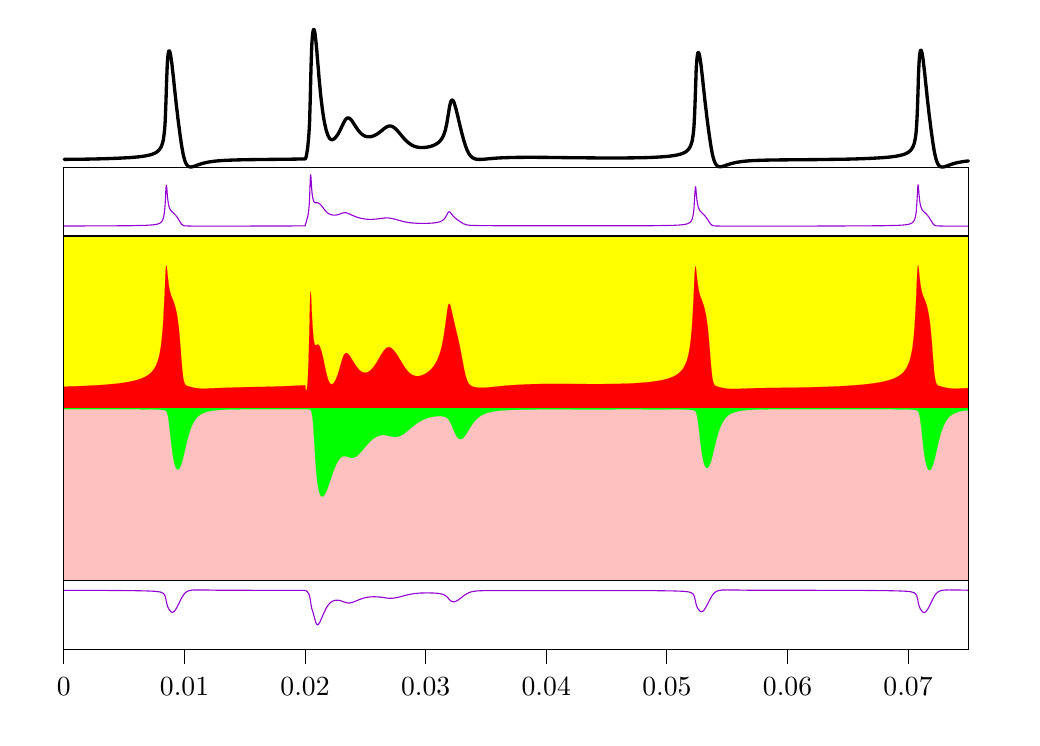
\begin{tikzpicture}[gnuplot]
%% generated with GNUPLOT 5.2p8 (Lua 5.3; terminal rev. Nov 2018, script rev. 108)
%% Wed Feb  3 22:37:26 2021
\path (0.000,0.000) rectangle (12.500,8.750);
\gpcolor{rgb color={0.000,0.000,0.000}}
\gpsetlinetype{gp lt border}
\gpsetdashtype{gp dt solid}
\gpsetlinewidth{3.00}
\draw[gp path] (0.464,7.097)--(0.468,7.097)--(0.471,7.097)--(0.475,7.097)--(0.479,7.097)%
  --(0.483,7.097)--(0.487,7.097)--(0.491,7.097)--(0.494,7.097)--(0.498,7.097)--(0.502,7.097)%
  --(0.506,7.097)--(0.510,7.097)--(0.514,7.097)--(0.517,7.098)--(0.521,7.098)--(0.525,7.098)%
  --(0.529,7.098)--(0.533,7.098)--(0.537,7.098)--(0.540,7.098)--(0.544,7.098)--(0.548,7.098)%
  --(0.552,7.098)--(0.556,7.098)--(0.560,7.098)--(0.563,7.098)--(0.567,7.098)--(0.571,7.098)%
  --(0.575,7.098)--(0.579,7.098)--(0.583,7.098)--(0.586,7.098)--(0.590,7.098)--(0.594,7.098)%
  --(0.598,7.099)--(0.602,7.099)--(0.606,7.099)--(0.609,7.099)--(0.613,7.099)--(0.617,7.099)%
  --(0.621,7.099)--(0.625,7.099)--(0.628,7.099)--(0.632,7.099)--(0.636,7.099)--(0.640,7.099)%
  --(0.644,7.099)--(0.648,7.099)--(0.651,7.099)--(0.655,7.099)--(0.659,7.099)--(0.663,7.099)%
  --(0.667,7.100)--(0.671,7.100)--(0.674,7.100)--(0.678,7.100)--(0.682,7.100)--(0.686,7.100)%
  --(0.690,7.100)--(0.694,7.100)--(0.697,7.100)--(0.701,7.100)--(0.705,7.100)--(0.709,7.100)%
  --(0.713,7.100)--(0.717,7.100)--(0.720,7.100)--(0.724,7.100)--(0.728,7.100)--(0.732,7.101)%
  --(0.736,7.101)--(0.740,7.101)--(0.743,7.101)--(0.747,7.101)--(0.751,7.101)--(0.755,7.101)%
  --(0.759,7.101)--(0.762,7.101)--(0.766,7.101)--(0.770,7.101)--(0.774,7.101)--(0.778,7.101)%
  --(0.782,7.101)--(0.785,7.102)--(0.789,7.102)--(0.793,7.102)--(0.797,7.102)--(0.801,7.102)%
  --(0.805,7.102)--(0.808,7.102)--(0.812,7.102)--(0.816,7.102)--(0.820,7.102)--(0.824,7.102)%
  --(0.828,7.102)--(0.831,7.102)--(0.835,7.102)--(0.839,7.103)--(0.843,7.103)--(0.847,7.103)%
  --(0.851,7.103)--(0.854,7.103)--(0.858,7.103)--(0.862,7.103)--(0.866,7.103)--(0.870,7.103)%
  --(0.874,7.103)--(0.877,7.103)--(0.881,7.103)--(0.885,7.104)--(0.889,7.104)--(0.893,7.104)%
  --(0.897,7.104)--(0.900,7.104)--(0.904,7.104)--(0.908,7.104)--(0.912,7.104)--(0.916,7.104)%
  --(0.919,7.104)--(0.923,7.105)--(0.927,7.105)--(0.931,7.105)--(0.935,7.105)--(0.939,7.105)%
  --(0.942,7.105)--(0.946,7.105)--(0.950,7.105)--(0.954,7.105)--(0.958,7.105)--(0.962,7.106)%
  --(0.965,7.106)--(0.969,7.106)--(0.973,7.106)--(0.977,7.106)--(0.981,7.106)--(0.985,7.106)%
  --(0.988,7.106)--(0.992,7.106)--(0.996,7.106)--(1.000,7.107)--(1.004,7.107)--(1.008,7.107)%
  --(1.011,7.107)--(1.015,7.107)--(1.019,7.107)--(1.023,7.107)--(1.027,7.107)--(1.031,7.108)%
  --(1.034,7.108)--(1.038,7.108)--(1.042,7.108)--(1.046,7.108)--(1.050,7.108)--(1.053,7.108)%
  --(1.057,7.108)--(1.061,7.109)--(1.065,7.109)--(1.069,7.109)--(1.073,7.109)--(1.076,7.109)%
  --(1.080,7.109)--(1.084,7.109)--(1.088,7.110)--(1.092,7.110)--(1.096,7.110)--(1.099,7.110)%
  --(1.103,7.110)--(1.107,7.110)--(1.111,7.110)--(1.115,7.111)--(1.119,7.111)--(1.122,7.111)%
  --(1.126,7.111)--(1.130,7.111)--(1.134,7.111)--(1.138,7.112)--(1.142,7.112)--(1.145,7.112)%
  --(1.149,7.112)--(1.153,7.112)--(1.157,7.112)--(1.161,7.113)--(1.165,7.113)--(1.168,7.113)%
  --(1.172,7.113)--(1.176,7.113)--(1.180,7.113)--(1.184,7.114)--(1.188,7.114)--(1.191,7.114)%
  --(1.195,7.114)--(1.199,7.114)--(1.203,7.115)--(1.207,7.115)--(1.210,7.115)--(1.214,7.115)%
  --(1.218,7.115)--(1.222,7.116)--(1.226,7.116)--(1.230,7.116)--(1.233,7.116)--(1.237,7.116)%
  --(1.241,7.117)--(1.245,7.117)--(1.249,7.117)--(1.253,7.117)--(1.256,7.117)--(1.260,7.118)%
  --(1.264,7.118)--(1.268,7.118)--(1.272,7.118)--(1.276,7.119)--(1.279,7.119)--(1.283,7.119)%
  --(1.287,7.119)--(1.291,7.120)--(1.295,7.120)--(1.299,7.120)--(1.302,7.120)--(1.306,7.121)%
  --(1.310,7.121)--(1.314,7.121)--(1.318,7.122)--(1.322,7.122)--(1.325,7.122)--(1.329,7.122)%
  --(1.333,7.123)--(1.337,7.123)--(1.341,7.123)--(1.344,7.124)--(1.348,7.124)--(1.352,7.124)%
  --(1.356,7.125)--(1.360,7.125)--(1.364,7.125)--(1.367,7.126)--(1.371,7.126)--(1.375,7.126)%
  --(1.379,7.127)--(1.383,7.127)--(1.387,7.127)--(1.390,7.128)--(1.394,7.128)--(1.398,7.129)%
  --(1.402,7.129)--(1.406,7.129)--(1.410,7.130)--(1.413,7.130)--(1.417,7.131)--(1.421,7.131)%
  --(1.425,7.132)--(1.429,7.132)--(1.433,7.133)--(1.436,7.133)--(1.440,7.133)--(1.444,7.134)%
  --(1.448,7.134)--(1.452,7.135)--(1.456,7.135)--(1.459,7.136)--(1.463,7.137)--(1.467,7.137)%
  --(1.471,7.138)--(1.475,7.138)--(1.479,7.139)--(1.482,7.140)--(1.486,7.140)--(1.490,7.141)%
  --(1.494,7.141)--(1.498,7.142)--(1.501,7.143)--(1.505,7.144)--(1.509,7.144)--(1.513,7.145)%
  --(1.517,7.146)--(1.521,7.147)--(1.524,7.147)--(1.528,7.148)--(1.532,7.149)--(1.536,7.150)%
  --(1.540,7.151)--(1.544,7.152)--(1.547,7.153)--(1.551,7.154)--(1.555,7.155)--(1.559,7.156)%
  --(1.563,7.157)--(1.567,7.158)--(1.570,7.159)--(1.574,7.160)--(1.578,7.162)--(1.582,7.163)%
  --(1.586,7.164)--(1.590,7.166)--(1.593,7.167)--(1.597,7.169)--(1.601,7.170)--(1.605,7.172)%
  --(1.609,7.174)--(1.613,7.176)--(1.616,7.177)--(1.620,7.179)--(1.624,7.182)--(1.628,7.184)%
  --(1.632,7.186)--(1.636,7.188)--(1.639,7.191)--(1.643,7.194)--(1.647,7.197)--(1.651,7.200)%
  --(1.655,7.203)--(1.658,7.206)--(1.662,7.210)--(1.666,7.214)--(1.670,7.218)--(1.674,7.223)%
  --(1.678,7.228)--(1.681,7.233)--(1.685,7.239)--(1.689,7.246)--(1.693,7.253)--(1.697,7.261)%
  --(1.701,7.269)--(1.704,7.279)--(1.708,7.290)--(1.712,7.303)--(1.716,7.317)--(1.720,7.334)%
  --(1.724,7.353)--(1.727,7.376)--(1.731,7.403)--(1.735,7.436)--(1.739,7.477)--(1.743,7.528)%
  --(1.747,7.592)--(1.750,7.673)--(1.754,7.774)--(1.758,7.891)--(1.762,8.016)--(1.766,8.133)%
  --(1.770,8.231)--(1.773,8.309)--(1.777,8.368)--(1.781,8.411)--(1.785,8.442)--(1.789,8.462)%
  --(1.792,8.473)--(1.796,8.477)--(1.800,8.475)--(1.804,8.468)--(1.808,8.455)--(1.812,8.439)%
  --(1.815,8.419)--(1.819,8.396)--(1.823,8.371)--(1.827,8.343)--(1.831,8.313)--(1.835,8.281)%
  --(1.838,8.248)--(1.842,8.214)--(1.846,8.179)--(1.850,8.143)--(1.854,8.107)--(1.858,8.071)%
  --(1.861,8.035)--(1.865,7.998)--(1.869,7.962)--(1.873,7.926)--(1.877,7.891)--(1.881,7.856)%
  --(1.884,7.821)--(1.888,7.787)--(1.892,7.753)--(1.896,7.720)--(1.900,7.688)--(1.904,7.656)%
  --(1.907,7.624)--(1.911,7.594)--(1.915,7.563)--(1.919,7.533)--(1.923,7.504)--(1.927,7.475)%
  --(1.930,7.446)--(1.934,7.418)--(1.938,7.391)--(1.942,7.364)--(1.946,7.337)--(1.949,7.311)%
  --(1.953,7.286)--(1.957,7.262)--(1.961,7.239)--(1.965,7.217)--(1.969,7.196)--(1.972,7.176)%
  --(1.976,7.158)--(1.980,7.140)--(1.984,7.124)--(1.988,7.110)--(1.992,7.096)--(1.995,7.084)%
  --(1.999,7.073)--(2.003,7.063)--(2.007,7.054)--(2.011,7.046)--(2.015,7.039)--(2.018,7.033)%
  --(2.022,7.027)--(2.026,7.022)--(2.030,7.018)--(2.034,7.015)--(2.038,7.012)--(2.041,7.009)%
  --(2.045,7.007)--(2.049,7.005)--(2.053,7.004)--(2.057,7.003)--(2.061,7.002)--(2.064,7.002)%
  --(2.068,7.001)--(2.072,7.001)--(2.076,7.001)--(2.080,7.002)--(2.083,7.002)--(2.087,7.003)%
  --(2.091,7.004)--(2.095,7.005)--(2.099,7.006)--(2.103,7.007)--(2.106,7.008)--(2.110,7.009)%
  --(2.114,7.010)--(2.118,7.011)--(2.122,7.013)--(2.126,7.014)--(2.129,7.015)--(2.133,7.017)%
  --(2.137,7.018)--(2.141,7.019)--(2.145,7.021)--(2.149,7.022)--(2.152,7.024)--(2.156,7.025)%
  --(2.160,7.026)--(2.164,7.028)--(2.168,7.029)--(2.172,7.030)--(2.175,7.032)--(2.179,7.033)%
  --(2.183,7.034)--(2.187,7.035)--(2.191,7.037)--(2.195,7.038)--(2.198,7.039)--(2.202,7.040)%
  --(2.206,7.042)--(2.210,7.043)--(2.214,7.044)--(2.218,7.045)--(2.221,7.046)--(2.225,7.047)%
  --(2.229,7.048)--(2.233,7.049)--(2.237,7.050)--(2.240,7.051)--(2.244,7.052)--(2.248,7.053)%
  --(2.252,7.054)--(2.256,7.055)--(2.260,7.056)--(2.263,7.056)--(2.267,7.057)--(2.271,7.058)%
  --(2.275,7.059)--(2.279,7.060)--(2.283,7.060)--(2.286,7.061)--(2.290,7.062)--(2.294,7.063)%
  --(2.298,7.063)--(2.302,7.064)--(2.306,7.065)--(2.309,7.065)--(2.313,7.066)--(2.317,7.067)%
  --(2.321,7.067)--(2.325,7.068)--(2.329,7.068)--(2.332,7.069)--(2.336,7.069)--(2.340,7.070)%
  --(2.344,7.070)--(2.348,7.071)--(2.352,7.071)--(2.355,7.072)--(2.359,7.072)--(2.363,7.073)%
  --(2.367,7.073)--(2.371,7.074)--(2.375,7.074)--(2.378,7.075)--(2.382,7.075)--(2.386,7.076)%
  --(2.390,7.076)--(2.394,7.076)--(2.397,7.077)--(2.401,7.077)--(2.405,7.077)--(2.409,7.078)%
  --(2.413,7.078)--(2.417,7.078)--(2.420,7.079)--(2.424,7.079)--(2.428,7.079)--(2.432,7.080)%
  --(2.436,7.080)--(2.440,7.080)--(2.443,7.081)--(2.447,7.081)--(2.451,7.081)--(2.455,7.082)%
  --(2.459,7.082)--(2.463,7.082)--(2.466,7.082)--(2.470,7.083)--(2.474,7.083)--(2.478,7.083)%
  --(2.482,7.083)--(2.486,7.084)--(2.489,7.084)--(2.493,7.084)--(2.497,7.084)--(2.501,7.084)%
  --(2.505,7.085)--(2.509,7.085)--(2.512,7.085)--(2.516,7.085)--(2.520,7.085)--(2.524,7.086)%
  --(2.528,7.086)--(2.531,7.086)--(2.535,7.086)--(2.539,7.086)--(2.543,7.087)--(2.547,7.087)%
  --(2.551,7.087)--(2.554,7.087)--(2.558,7.087)--(2.562,7.087)--(2.566,7.087)--(2.570,7.088)%
  --(2.574,7.088)--(2.577,7.088)--(2.581,7.088)--(2.585,7.088)--(2.589,7.088)--(2.593,7.088)%
  --(2.597,7.089)--(2.600,7.089)--(2.604,7.089)--(2.608,7.089)--(2.612,7.089)--(2.616,7.089)%
  --(2.620,7.089)--(2.623,7.089)--(2.627,7.090)--(2.631,7.090)--(2.635,7.090)--(2.639,7.090)%
  --(2.643,7.090)--(2.646,7.090)--(2.650,7.090)--(2.654,7.090)--(2.658,7.090)--(2.662,7.091)%
  --(2.666,7.091)--(2.669,7.091)--(2.673,7.091)--(2.677,7.091)--(2.681,7.091)--(2.685,7.091)%
  --(2.688,7.091)--(2.692,7.091)--(2.696,7.091)--(2.700,7.091)--(2.704,7.092)--(2.708,7.092)%
  --(2.711,7.092)--(2.715,7.092)--(2.719,7.092)--(2.723,7.092)--(2.727,7.092)--(2.731,7.092)%
  --(2.734,7.092)--(2.738,7.092)--(2.742,7.092)--(2.746,7.092)--(2.750,7.092)--(2.754,7.093)%
  --(2.757,7.093)--(2.761,7.093)--(2.765,7.093)--(2.769,7.093)--(2.773,7.093)--(2.777,7.093)%
  --(2.780,7.093)--(2.784,7.093)--(2.788,7.093)--(2.792,7.093)--(2.796,7.093)--(2.800,7.093)%
  --(2.803,7.093)--(2.807,7.093)--(2.811,7.093)--(2.815,7.094)--(2.819,7.094)--(2.822,7.094)%
  --(2.826,7.094)--(2.830,7.094)--(2.834,7.094)--(2.838,7.094)--(2.842,7.094)--(2.845,7.094)%
  --(2.849,7.094)--(2.853,7.094)--(2.857,7.094)--(2.861,7.094)--(2.865,7.094)--(2.868,7.094)%
  --(2.872,7.094)--(2.876,7.094)--(2.880,7.094)--(2.884,7.094)--(2.888,7.095)--(2.891,7.095)%
  --(2.895,7.095)--(2.899,7.095)--(2.903,7.095)--(2.907,7.095)--(2.911,7.095)--(2.914,7.095)%
  --(2.918,7.095)--(2.922,7.095)--(2.926,7.095)--(2.930,7.095)--(2.934,7.095)--(2.937,7.095)%
  --(2.941,7.095)--(2.945,7.095)--(2.949,7.095)--(2.953,7.095)--(2.957,7.095)--(2.960,7.095)%
  --(2.964,7.095)--(2.968,7.095)--(2.972,7.096)--(2.976,7.096)--(2.979,7.096)--(2.983,7.096)%
  --(2.987,7.096)--(2.991,7.096)--(2.995,7.096)--(2.999,7.096)--(3.002,7.096)--(3.006,7.096)%
  --(3.010,7.096)--(3.014,7.096)--(3.018,7.096)--(3.022,7.096)--(3.025,7.096)--(3.029,7.096)%
  --(3.033,7.096)--(3.037,7.096)--(3.041,7.096)--(3.045,7.096)--(3.048,7.096)--(3.052,7.096)%
  --(3.056,7.096)--(3.060,7.097)--(3.064,7.097)--(3.068,7.097)--(3.071,7.097)--(3.075,7.097)%
  --(3.079,7.097)--(3.083,7.097)--(3.087,7.097)--(3.091,7.097)--(3.094,7.097)--(3.098,7.097)%
  --(3.102,7.097)--(3.106,7.097)--(3.110,7.097)--(3.113,7.097)--(3.117,7.097)--(3.121,7.097)%
  --(3.125,7.097)--(3.129,7.097)--(3.133,7.097)--(3.136,7.097)--(3.140,7.097)--(3.144,7.097)%
  --(3.148,7.098)--(3.152,7.098)--(3.156,7.098)--(3.159,7.098)--(3.163,7.098)--(3.167,7.098)%
  --(3.171,7.098)--(3.175,7.098)--(3.179,7.098)--(3.182,7.098)--(3.186,7.098)--(3.190,7.098)%
  --(3.194,7.098)--(3.198,7.098)--(3.202,7.098)--(3.205,7.098)--(3.209,7.098)--(3.213,7.098)%
  --(3.217,7.098)--(3.221,7.098)--(3.225,7.099)--(3.228,7.099)--(3.232,7.099)--(3.236,7.099)%
  --(3.240,7.099)--(3.244,7.099)--(3.248,7.099)--(3.251,7.099)--(3.255,7.099)--(3.259,7.099)%
  --(3.263,7.099)--(3.267,7.099)--(3.270,7.099)--(3.274,7.099)--(3.278,7.099)--(3.282,7.099)%
  --(3.286,7.099)--(3.290,7.099)--(3.293,7.099)--(3.297,7.100)--(3.301,7.100)--(3.305,7.100)%
  --(3.309,7.100)--(3.313,7.100)--(3.316,7.100)--(3.320,7.100)--(3.324,7.100)--(3.328,7.100)%
  --(3.332,7.100)--(3.336,7.100)--(3.339,7.100)--(3.343,7.100)--(3.347,7.100)--(3.351,7.100)%
  --(3.355,7.100)--(3.359,7.101)--(3.362,7.101)--(3.366,7.101)--(3.370,7.101)--(3.374,7.101)%
  --(3.378,7.101)--(3.382,7.101)--(3.385,7.101)--(3.389,7.101)--(3.393,7.101)--(3.397,7.101)%
  --(3.401,7.101)--(3.405,7.101)--(3.408,7.101)--(3.412,7.101)--(3.416,7.102)--(3.420,7.102)%
  --(3.424,7.102)--(3.427,7.102)--(3.431,7.102)--(3.435,7.102)--(3.439,7.102)--(3.443,7.102)%
  --(3.447,7.102)--(3.450,7.102)--(3.454,7.102)--(3.458,7.102)--(3.462,7.102)--(3.466,7.103)%
  --(3.470,7.103)--(3.473,7.103)--(3.477,7.103)--(3.481,7.103)--(3.485,7.103)--(3.489,7.103)%
  --(3.493,7.103)--(3.496,7.103)--(3.500,7.103)--(3.504,7.103)--(3.508,7.103)--(3.512,7.104)%
  --(3.516,7.104)--(3.519,7.104)--(3.523,7.104)--(3.527,7.106)--(3.531,7.114)--(3.535,7.125)%
  --(3.539,7.140)--(3.542,7.159)--(3.546,7.180)--(3.550,7.205)--(3.554,7.232)--(3.558,7.263)%
  --(3.561,7.298)--(3.565,7.338)--(3.569,7.385)--(3.573,7.440)--(3.577,7.508)--(3.581,7.593)%
  --(3.584,7.702)--(3.588,7.841)--(3.592,8.003)--(3.596,8.169)--(3.600,8.314)--(3.604,8.432)%
  --(3.607,8.523)--(3.611,8.595)--(3.615,8.649)--(3.619,8.689)--(3.623,8.718)--(3.627,8.737)%
  --(3.630,8.747)--(3.634,8.749)--(3.638,8.744)--(3.642,8.732)--(3.646,8.714)--(3.650,8.691)%
  --(3.653,8.662)--(3.657,8.630)--(3.661,8.593)--(3.665,8.553)--(3.669,8.511)--(3.673,8.467)%
  --(3.676,8.422)--(3.680,8.376)--(3.684,8.329)--(3.688,8.283)--(3.692,8.237)--(3.696,8.192)%
  --(3.699,8.147)--(3.703,8.104)--(3.707,8.061)--(3.711,8.020)--(3.715,7.981)--(3.718,7.943)%
  --(3.722,7.906)--(3.726,7.871)--(3.730,7.837)--(3.734,7.805)--(3.738,7.774)--(3.741,7.744)%
  --(3.745,7.716)--(3.749,7.689)--(3.753,7.663)--(3.757,7.639)--(3.761,7.616)--(3.764,7.594)%
  --(3.768,7.573)--(3.772,7.553)--(3.776,7.534)--(3.780,7.517)--(3.784,7.500)--(3.787,7.484)%
  --(3.791,7.469)--(3.795,7.456)--(3.799,7.443)--(3.803,7.431)--(3.807,7.420)--(3.810,7.410)%
  --(3.814,7.401)--(3.818,7.392)--(3.822,7.385)--(3.826,7.378)--(3.830,7.372)--(3.833,7.367)%
  --(3.837,7.362)--(3.841,7.358)--(3.845,7.355)--(3.849,7.352)--(3.852,7.350)--(3.856,7.349)%
  --(3.860,7.348)--(3.864,7.348)--(3.868,7.348)--(3.872,7.349)--(3.875,7.350)--(3.879,7.351)%
  --(3.883,7.353)--(3.887,7.355)--(3.891,7.358)--(3.895,7.361)--(3.898,7.364)--(3.902,7.368)%
  --(3.906,7.372)--(3.910,7.376)--(3.914,7.380)--(3.918,7.385)--(3.921,7.390)--(3.925,7.395)%
  --(3.929,7.401)--(3.933,7.406)--(3.937,7.412)--(3.941,7.418)--(3.944,7.425)--(3.948,7.431)%
  --(3.952,7.438)--(3.956,7.445)--(3.960,7.452)--(3.964,7.460)--(3.967,7.467)--(3.971,7.475)%
  --(3.975,7.483)--(3.979,7.491)--(3.983,7.499)--(3.987,7.507)--(3.990,7.515)--(3.994,7.523)%
  --(3.998,7.531)--(4.002,7.539)--(4.006,7.547)--(4.009,7.555)--(4.013,7.563)--(4.017,7.570)%
  --(4.021,7.577)--(4.025,7.584)--(4.029,7.590)--(4.032,7.596)--(4.036,7.602)--(4.040,7.606)%
  --(4.044,7.611)--(4.048,7.614)--(4.052,7.617)--(4.055,7.620)--(4.059,7.622)--(4.063,7.623)%
  --(4.067,7.624)--(4.071,7.624)--(4.075,7.623)--(4.078,7.622)--(4.082,7.621)--(4.086,7.619)%
  --(4.090,7.616)--(4.094,7.613)--(4.098,7.610)--(4.101,7.606)--(4.105,7.602)--(4.109,7.597)%
  --(4.113,7.593)--(4.117,7.588)--(4.121,7.582)--(4.124,7.577)--(4.128,7.571)--(4.132,7.566)%
  --(4.136,7.560)--(4.140,7.554)--(4.143,7.548)--(4.147,7.542)--(4.151,7.536)--(4.155,7.530)%
  --(4.159,7.524)--(4.163,7.518)--(4.166,7.512)--(4.170,7.507)--(4.174,7.501)--(4.178,7.495)%
  --(4.182,7.490)--(4.186,7.484)--(4.189,7.479)--(4.193,7.474)--(4.197,7.468)--(4.201,7.464)%
  --(4.205,7.459)--(4.209,7.454)--(4.212,7.449)--(4.216,7.445)--(4.220,7.441)--(4.224,7.437)%
  --(4.228,7.433)--(4.232,7.429)--(4.235,7.425)--(4.239,7.422)--(4.243,7.419)--(4.247,7.416)%
  --(4.251,7.413)--(4.255,7.410)--(4.258,7.407)--(4.262,7.405)--(4.266,7.402)--(4.270,7.400)%
  --(4.274,7.398)--(4.278,7.396)--(4.281,7.394)--(4.285,7.393)--(4.289,7.391)--(4.293,7.390)%
  --(4.297,7.389)--(4.300,7.388)--(4.304,7.387)--(4.308,7.386)--(4.312,7.385)--(4.316,7.385)%
  --(4.320,7.384)--(4.323,7.384)--(4.327,7.384)--(4.331,7.384)--(4.335,7.384)--(4.339,7.384)%
  --(4.343,7.384)--(4.346,7.385)--(4.350,7.385)--(4.354,7.386)--(4.358,7.386)--(4.362,7.387)%
  --(4.366,7.388)--(4.369,7.389)--(4.373,7.390)--(4.377,7.391)--(4.381,7.392)--(4.385,7.393)%
  --(4.389,7.395)--(4.392,7.396)--(4.396,7.398)--(4.400,7.399)--(4.404,7.401)--(4.408,7.403)%
  --(4.412,7.405)--(4.415,7.407)--(4.419,7.409)--(4.423,7.411)--(4.427,7.413)--(4.431,7.415)%
  --(4.435,7.417)--(4.438,7.420)--(4.442,7.422)--(4.446,7.425)--(4.450,7.427)--(4.454,7.430)%
  --(4.457,7.433)--(4.461,7.435)--(4.465,7.438)--(4.469,7.441)--(4.473,7.444)--(4.477,7.447)%
  --(4.480,7.450)--(4.484,7.453)--(4.488,7.456)--(4.492,7.459)--(4.496,7.462)--(4.500,7.465)%
  --(4.503,7.468)--(4.507,7.472)--(4.511,7.475)--(4.515,7.478)--(4.519,7.481)--(4.523,7.484)%
  --(4.526,7.487)--(4.530,7.490)--(4.534,7.493)--(4.538,7.495)--(4.542,7.498)--(4.546,7.501)%
  --(4.549,7.503)--(4.553,7.505)--(4.557,7.508)--(4.561,7.510)--(4.565,7.512)--(4.569,7.513)%
  --(4.572,7.515)--(4.576,7.517)--(4.580,7.518)--(4.584,7.519)--(4.588,7.520)--(4.591,7.520)%
  --(4.595,7.521)--(4.599,7.521)--(4.603,7.521)--(4.607,7.521)--(4.611,7.520)--(4.614,7.520)%
  --(4.618,7.519)--(4.622,7.518)--(4.626,7.516)--(4.630,7.515)--(4.634,7.513)--(4.637,7.511)%
  --(4.641,7.509)--(4.645,7.506)--(4.649,7.504)--(4.653,7.501)--(4.657,7.498)--(4.660,7.495)%
  --(4.664,7.492)--(4.668,7.489)--(4.672,7.485)--(4.676,7.482)--(4.680,7.478)--(4.683,7.474)%
  --(4.687,7.470)--(4.691,7.466)--(4.695,7.462)--(4.699,7.458)--(4.703,7.453)--(4.706,7.449)%
  --(4.710,7.445)--(4.714,7.440)--(4.718,7.436)--(4.722,7.431)--(4.726,7.427)--(4.729,7.422)%
  --(4.733,7.417)--(4.737,7.413)--(4.741,7.408)--(4.745,7.404)--(4.748,7.399)--(4.752,7.395)%
  --(4.756,7.390)--(4.760,7.386)--(4.764,7.381)--(4.768,7.377)--(4.771,7.372)--(4.775,7.368)%
  --(4.779,7.364)--(4.783,7.359)--(4.787,7.355)--(4.791,7.351)--(4.794,7.347)--(4.798,7.343)%
  --(4.802,7.339)--(4.806,7.336)--(4.810,7.332)--(4.814,7.328)--(4.817,7.325)--(4.821,7.321)%
  --(4.825,7.318)--(4.829,7.314)--(4.833,7.311)--(4.837,7.308)--(4.840,7.305)--(4.844,7.302)%
  --(4.848,7.299)--(4.852,7.296)--(4.856,7.294)--(4.860,7.291)--(4.863,7.288)--(4.867,7.286)%
  --(4.871,7.284)--(4.875,7.281)--(4.879,7.279)--(4.882,7.277)--(4.886,7.275)--(4.890,7.273)%
  --(4.894,7.271)--(4.898,7.270)--(4.902,7.268)--(4.905,7.266)--(4.909,7.265)--(4.913,7.263)%
  --(4.917,7.262)--(4.921,7.261)--(4.925,7.260)--(4.928,7.258)--(4.932,7.257)--(4.936,7.256)%
  --(4.940,7.255)--(4.944,7.254)--(4.948,7.254)--(4.951,7.253)--(4.955,7.252)--(4.959,7.251)%
  --(4.963,7.251)--(4.967,7.250)--(4.971,7.250)--(4.974,7.249)--(4.978,7.249)--(4.982,7.249)%
  --(4.986,7.248)--(4.990,7.248)--(4.994,7.248)--(4.997,7.248)--(5.001,7.248)--(5.005,7.248)%
  --(5.009,7.248)--(5.013,7.248)--(5.017,7.248)--(5.020,7.248)--(5.024,7.248)--(5.028,7.248)%
  --(5.032,7.248)--(5.036,7.249)--(5.039,7.249)--(5.043,7.249)--(5.047,7.250)--(5.051,7.250)%
  --(5.055,7.250)--(5.059,7.251)--(5.062,7.251)--(5.066,7.252)--(5.070,7.253)--(5.074,7.253)%
  --(5.078,7.254)--(5.082,7.254)--(5.085,7.255)--(5.089,7.256)--(5.093,7.257)--(5.097,7.258)%
  --(5.101,7.258)--(5.105,7.259)--(5.108,7.260)--(5.112,7.261)--(5.116,7.262)--(5.120,7.263)%
  --(5.124,7.265)--(5.128,7.266)--(5.131,7.267)--(5.135,7.268)--(5.139,7.270)--(5.143,7.271)%
  --(5.147,7.272)--(5.151,7.274)--(5.154,7.275)--(5.158,7.277)--(5.162,7.279)--(5.166,7.280)%
  --(5.170,7.282)--(5.173,7.284)--(5.177,7.286)--(5.181,7.288)--(5.185,7.290)--(5.189,7.293)%
  --(5.193,7.295)--(5.196,7.297)--(5.200,7.300)--(5.204,7.303)--(5.208,7.305)--(5.212,7.308)%
  --(5.216,7.311)--(5.219,7.315)--(5.223,7.318)--(5.227,7.322)--(5.231,7.325)--(5.235,7.329)%
  --(5.239,7.333)--(5.242,7.338)--(5.246,7.343)--(5.250,7.348)--(5.254,7.353)--(5.258,7.359)%
  --(5.262,7.365)--(5.265,7.371)--(5.269,7.378)--(5.273,7.385)--(5.277,7.393)--(5.281,7.402)%
  --(5.285,7.411)--(5.288,7.421)--(5.292,7.432)--(5.296,7.443)--(5.300,7.456)--(5.304,7.469)%
  --(5.308,7.484)--(5.311,7.500)--(5.315,7.517)--(5.319,7.535)--(5.323,7.555)--(5.327,7.575)%
  --(5.330,7.598)--(5.334,7.621)--(5.338,7.644)--(5.342,7.669)--(5.346,7.693)--(5.350,7.717)%
  --(5.353,7.740)--(5.357,7.761)--(5.361,7.781)--(5.365,7.798)--(5.369,7.813)--(5.373,7.825)%
  --(5.376,7.835)--(5.380,7.843)--(5.384,7.848)--(5.388,7.851)--(5.392,7.851)--(5.396,7.850)%
  --(5.399,7.846)--(5.403,7.841)--(5.407,7.835)--(5.411,7.827)--(5.415,7.818)--(5.419,7.808)%
  --(5.422,7.796)--(5.426,7.784)--(5.430,7.771)--(5.434,7.758)--(5.438,7.744)--(5.442,7.729)%
  --(5.445,7.714)--(5.449,7.699)--(5.453,7.683)--(5.457,7.667)--(5.461,7.651)--(5.465,7.635)%
  --(5.468,7.619)--(5.472,7.603)--(5.476,7.586)--(5.480,7.570)--(5.484,7.554)--(5.487,7.538)%
  --(5.491,7.522)--(5.495,7.506)--(5.499,7.490)--(5.503,7.475)--(5.507,7.459)--(5.510,7.444)%
  --(5.514,7.429)--(5.518,7.414)--(5.522,7.400)--(5.526,7.385)--(5.530,7.371)--(5.533,7.357)%
  --(5.537,7.344)--(5.541,7.331)--(5.545,7.318)--(5.549,7.305)--(5.553,7.293)--(5.556,7.281)%
  --(5.560,7.270)--(5.564,7.259)--(5.568,7.248)--(5.572,7.238)--(5.576,7.229)--(5.579,7.219)%
  --(5.583,7.211)--(5.587,7.202)--(5.591,7.194)--(5.595,7.187)--(5.599,7.180)--(5.602,7.173)%
  --(5.606,7.167)--(5.610,7.161)--(5.614,7.156)--(5.618,7.150)--(5.621,7.146)--(5.625,7.141)%
  --(5.629,7.137)--(5.633,7.133)--(5.637,7.129)--(5.641,7.126)--(5.644,7.123)--(5.648,7.120)%
  --(5.652,7.118)--(5.656,7.115)--(5.660,7.113)--(5.664,7.111)--(5.667,7.109)--(5.671,7.108)%
  --(5.675,7.106)--(5.679,7.105)--(5.683,7.104)--(5.687,7.102)--(5.690,7.101)--(5.694,7.101)%
  --(5.698,7.100)--(5.702,7.099)--(5.706,7.099)--(5.710,7.098)--(5.713,7.098)--(5.717,7.097)%
  --(5.721,7.097)--(5.725,7.097)--(5.729,7.097)--(5.733,7.097)--(5.736,7.097)--(5.740,7.097)%
  --(5.744,7.097)--(5.748,7.097)--(5.752,7.097)--(5.756,7.097)--(5.759,7.097)--(5.763,7.097)%
  --(5.767,7.097)--(5.771,7.098)--(5.775,7.098)--(5.778,7.098)--(5.782,7.098)--(5.786,7.099)%
  --(5.790,7.099)--(5.794,7.099)--(5.798,7.100)--(5.801,7.100)--(5.805,7.100)--(5.809,7.101)%
  --(5.813,7.101)--(5.817,7.101)--(5.821,7.102)--(5.824,7.102)--(5.828,7.102)--(5.832,7.103)%
  --(5.836,7.103)--(5.840,7.103)--(5.844,7.104)--(5.847,7.104)--(5.851,7.105)--(5.855,7.105)%
  --(5.859,7.105)--(5.863,7.106)--(5.867,7.106)--(5.870,7.106)--(5.874,7.107)--(5.878,7.107)%
  --(5.882,7.107)--(5.886,7.108)--(5.890,7.108)--(5.893,7.108)--(5.897,7.109)--(5.901,7.109)%
  --(5.905,7.109)--(5.909,7.110)--(5.912,7.110)--(5.916,7.110)--(5.920,7.111)--(5.924,7.111)%
  --(5.928,7.111)--(5.932,7.111)--(5.935,7.112)--(5.939,7.112)--(5.943,7.112)--(5.947,7.113)%
  --(5.951,7.113)--(5.955,7.113)--(5.958,7.113)--(5.962,7.114)--(5.966,7.114)--(5.970,7.114)%
  --(5.974,7.114)--(5.978,7.115)--(5.981,7.115)--(5.985,7.115)--(5.989,7.115)--(5.993,7.115)%
  --(5.997,7.116)--(6.001,7.116)--(6.004,7.116)--(6.008,7.116)--(6.012,7.116)--(6.016,7.117)%
  --(6.020,7.117)--(6.024,7.117)--(6.027,7.117)--(6.031,7.117)--(6.035,7.118)--(6.039,7.118)%
  --(6.043,7.118)--(6.047,7.118)--(6.050,7.118)--(6.054,7.118)--(6.058,7.119)--(6.062,7.119)%
  --(6.066,7.119)--(6.069,7.119)--(6.073,7.119)--(6.077,7.119)--(6.081,7.119)--(6.085,7.120)%
  --(6.089,7.120)--(6.092,7.120)--(6.096,7.120)--(6.100,7.120)--(6.104,7.120)--(6.108,7.120)%
  --(6.112,7.120)--(6.115,7.121)--(6.119,7.121)--(6.123,7.121)--(6.127,7.121)--(6.131,7.121)%
  --(6.135,7.121)--(6.138,7.121)--(6.142,7.121)--(6.146,7.121)--(6.150,7.121)--(6.154,7.122)%
  --(6.158,7.122)--(6.161,7.122)--(6.165,7.122)--(6.169,7.122)--(6.173,7.122)--(6.177,7.122)%
  --(6.181,7.122)--(6.184,7.122)--(6.188,7.122)--(6.192,7.122)--(6.196,7.122)--(6.200,7.122)%
  --(6.204,7.122)--(6.207,7.123)--(6.211,7.123)--(6.215,7.123)--(6.219,7.123)--(6.223,7.123)%
  --(6.226,7.123)--(6.230,7.123)--(6.234,7.123)--(6.238,7.123)--(6.242,7.123)--(6.246,7.123)%
  --(6.249,7.123)--(6.253,7.123)--(6.257,7.123)--(6.261,7.123)--(6.265,7.123)--(6.269,7.123)%
  --(6.272,7.123)--(6.276,7.123)--(6.280,7.123)--(6.284,7.123)--(6.288,7.123)--(6.292,7.123)%
  --(6.295,7.123)--(6.299,7.123)--(6.303,7.124)--(6.307,7.124)--(6.311,7.124)--(6.315,7.124)%
  --(6.318,7.124)--(6.322,7.124)--(6.326,7.124)--(6.330,7.124)--(6.334,7.124)--(6.338,7.124)%
  --(6.341,7.124)--(6.345,7.124)--(6.349,7.124)--(6.353,7.124)--(6.357,7.124)--(6.360,7.124)%
  --(6.364,7.124)--(6.368,7.124)--(6.372,7.124)--(6.376,7.124)--(6.380,7.124)--(6.383,7.124)%
  --(6.387,7.124)--(6.391,7.124)--(6.395,7.124)--(6.399,7.124)--(6.403,7.124)--(6.406,7.124)%
  --(6.410,7.124)--(6.414,7.124)--(6.418,7.124)--(6.422,7.124)--(6.426,7.124)--(6.429,7.124)%
  --(6.433,7.124)--(6.437,7.124)--(6.441,7.124)--(6.445,7.124)--(6.449,7.124)--(6.452,7.124)%
  --(6.456,7.124)--(6.460,7.124)--(6.464,7.124)--(6.468,7.123)--(6.472,7.123)--(6.475,7.123)%
  --(6.479,7.123)--(6.483,7.123)--(6.487,7.123)--(6.491,7.123)--(6.495,7.123)--(6.498,7.123)%
  --(6.502,7.123)--(6.506,7.123)--(6.510,7.123)--(6.514,7.123)--(6.517,7.123)--(6.521,7.123)%
  --(6.525,7.123)--(6.529,7.123)--(6.533,7.123)--(6.537,7.123)--(6.540,7.123)--(6.544,7.123)%
  --(6.548,7.123)--(6.552,7.123)--(6.556,7.123)--(6.560,7.123)--(6.563,7.123)--(6.567,7.123)%
  --(6.571,7.123)--(6.575,7.123)--(6.579,7.123)--(6.583,7.123)--(6.586,7.123)--(6.590,7.123)%
  --(6.594,7.123)--(6.598,7.123)--(6.602,7.122)--(6.606,7.122)--(6.609,7.122)--(6.613,7.122)%
  --(6.617,7.122)--(6.621,7.122)--(6.625,7.122)--(6.629,7.122)--(6.632,7.122)--(6.636,7.122)%
  --(6.640,7.122)--(6.644,7.122)--(6.648,7.122)--(6.651,7.122)--(6.655,7.122)--(6.659,7.122)%
  --(6.663,7.122)--(6.667,7.122)--(6.671,7.122)--(6.674,7.122)--(6.678,7.122)--(6.682,7.122)%
  --(6.686,7.122)--(6.690,7.122)--(6.694,7.121)--(6.697,7.121)--(6.701,7.121)--(6.705,7.121)%
  --(6.709,7.121)--(6.713,7.121)--(6.717,7.121)--(6.720,7.121)--(6.724,7.121)--(6.728,7.121)%
  --(6.732,7.121)--(6.736,7.121)--(6.740,7.121)--(6.743,7.121)--(6.747,7.121)--(6.751,7.121)%
  --(6.755,7.121)--(6.759,7.121)--(6.763,7.121)--(6.766,7.121)--(6.770,7.121)--(6.774,7.121)%
  --(6.778,7.120)--(6.782,7.120)--(6.786,7.120)--(6.789,7.120)--(6.793,7.120)--(6.797,7.120)%
  --(6.801,7.120)--(6.805,7.120)--(6.808,7.120)--(6.812,7.120)--(6.816,7.120)--(6.820,7.120)%
  --(6.824,7.120)--(6.828,7.120)--(6.831,7.120)--(6.835,7.120)--(6.839,7.120)--(6.843,7.120)%
  --(6.847,7.120)--(6.851,7.120)--(6.854,7.119)--(6.858,7.119)--(6.862,7.119)--(6.866,7.119)%
  --(6.870,7.119)--(6.874,7.119)--(6.877,7.119)--(6.881,7.119)--(6.885,7.119)--(6.889,7.119)%
  --(6.893,7.119)--(6.897,7.119)--(6.900,7.119)--(6.904,7.119)--(6.908,7.119)--(6.912,7.119)%
  --(6.916,7.119)--(6.920,7.119)--(6.923,7.119)--(6.927,7.119)--(6.931,7.118)--(6.935,7.118)%
  --(6.939,7.118)--(6.942,7.118)--(6.946,7.118)--(6.950,7.118)--(6.954,7.118)--(6.958,7.118)%
  --(6.962,7.118)--(6.965,7.118)--(6.969,7.118)--(6.973,7.118)--(6.977,7.118)--(6.981,7.118)%
  --(6.985,7.118)--(6.988,7.118)--(6.992,7.118)--(6.996,7.118)--(7.000,7.118)--(7.004,7.118)%
  --(7.008,7.118)--(7.011,7.118)--(7.015,7.117)--(7.019,7.117)--(7.023,7.117)--(7.027,7.117)%
  --(7.031,7.117)--(7.034,7.117)--(7.038,7.117)--(7.042,7.117)--(7.046,7.117)--(7.050,7.117)%
  --(7.054,7.117)--(7.057,7.117)--(7.061,7.117)--(7.065,7.117)--(7.069,7.117)--(7.073,7.117)%
  --(7.077,7.117)--(7.080,7.117)--(7.084,7.117)--(7.088,7.117)--(7.092,7.117)--(7.096,7.117)%
  --(7.099,7.117)--(7.103,7.116)--(7.107,7.116)--(7.111,7.116)--(7.115,7.116)--(7.119,7.116)%
  --(7.122,7.116)--(7.126,7.116)--(7.130,7.116)--(7.134,7.116)--(7.138,7.116)--(7.142,7.116)%
  --(7.145,7.116)--(7.149,7.116)--(7.153,7.116)--(7.157,7.116)--(7.161,7.116)--(7.165,7.116)%
  --(7.168,7.116)--(7.172,7.116)--(7.176,7.116)--(7.180,7.116)--(7.184,7.116)--(7.188,7.116)%
  --(7.191,7.116)--(7.195,7.116)--(7.199,7.116)--(7.203,7.116)--(7.207,7.116)--(7.211,7.115)%
  --(7.214,7.115)--(7.218,7.115)--(7.222,7.115)--(7.226,7.115)--(7.230,7.115)--(7.234,7.115)%
  --(7.237,7.115)--(7.241,7.115)--(7.245,7.115)--(7.249,7.115)--(7.253,7.115)--(7.256,7.115)%
  --(7.260,7.115)--(7.264,7.115)--(7.268,7.115)--(7.272,7.115)--(7.276,7.115)--(7.279,7.115)%
  --(7.283,7.115)--(7.287,7.115)--(7.291,7.115)--(7.295,7.115)--(7.299,7.115)--(7.302,7.115)%
  --(7.306,7.115)--(7.310,7.115)--(7.314,7.115)--(7.318,7.115)--(7.322,7.115)--(7.325,7.115)%
  --(7.329,7.115)--(7.333,7.115)--(7.337,7.115)--(7.341,7.115)--(7.345,7.115)--(7.348,7.115)%
  --(7.352,7.115)--(7.356,7.115)--(7.360,7.115)--(7.364,7.115)--(7.368,7.115)--(7.371,7.115)%
  --(7.375,7.115)--(7.379,7.115)--(7.383,7.115)--(7.387,7.115)--(7.390,7.115)--(7.394,7.115)%
  --(7.398,7.115)--(7.402,7.115)--(7.406,7.115)--(7.410,7.115)--(7.413,7.115)--(7.417,7.115)%
  --(7.421,7.115)--(7.425,7.115)--(7.429,7.115)--(7.433,7.115)--(7.436,7.115)--(7.440,7.115)%
  --(7.444,7.115)--(7.448,7.115)--(7.452,7.115)--(7.456,7.115)--(7.459,7.115)--(7.463,7.115)%
  --(7.467,7.115)--(7.471,7.115)--(7.475,7.115)--(7.479,7.115)--(7.482,7.115)--(7.486,7.115)%
  --(7.490,7.115)--(7.494,7.115)--(7.498,7.115)--(7.502,7.115)--(7.505,7.115)--(7.509,7.115)%
  --(7.513,7.115)--(7.517,7.115)--(7.521,7.115)--(7.525,7.115)--(7.528,7.115)--(7.532,7.115)%
  --(7.536,7.115)--(7.540,7.115)--(7.544,7.115)--(7.547,7.115)--(7.551,7.115)--(7.555,7.115)%
  --(7.559,7.115)--(7.563,7.115)--(7.567,7.115)--(7.570,7.115)--(7.574,7.115)--(7.578,7.115)%
  --(7.582,7.115)--(7.586,7.115)--(7.590,7.115)--(7.593,7.115)--(7.597,7.115)--(7.601,7.115)%
  --(7.605,7.115)--(7.609,7.115)--(7.613,7.115)--(7.616,7.115)--(7.620,7.116)--(7.624,7.116)%
  --(7.628,7.116)--(7.632,7.116)--(7.636,7.116)--(7.639,7.116)--(7.643,7.116)--(7.647,7.116)%
  --(7.651,7.116)--(7.655,7.116)--(7.659,7.116)--(7.662,7.116)--(7.666,7.116)--(7.670,7.116)%
  --(7.674,7.116)--(7.678,7.116)--(7.681,7.116)--(7.685,7.116)--(7.689,7.116)--(7.693,7.116)%
  --(7.697,7.116)--(7.701,7.117)--(7.704,7.117)--(7.708,7.117)--(7.712,7.117)--(7.716,7.117)%
  --(7.720,7.117)--(7.724,7.117)--(7.727,7.117)--(7.731,7.117)--(7.735,7.117)--(7.739,7.117)%
  --(7.743,7.117)--(7.747,7.117)--(7.750,7.117)--(7.754,7.118)--(7.758,7.118)--(7.762,7.118)%
  --(7.766,7.118)--(7.770,7.118)--(7.773,7.118)--(7.777,7.118)--(7.781,7.118)--(7.785,7.118)%
  --(7.789,7.118)--(7.793,7.118)--(7.796,7.118)--(7.800,7.119)--(7.804,7.119)--(7.808,7.119)%
  --(7.812,7.119)--(7.816,7.119)--(7.819,7.119)--(7.823,7.119)--(7.827,7.119)--(7.831,7.119)%
  --(7.835,7.119)--(7.838,7.120)--(7.842,7.120)--(7.846,7.120)--(7.850,7.120)--(7.854,7.120)%
  --(7.858,7.120)--(7.861,7.120)--(7.865,7.120)--(7.869,7.121)--(7.873,7.121)--(7.877,7.121)%
  --(7.881,7.121)--(7.884,7.121)--(7.888,7.121)--(7.892,7.121)--(7.896,7.121)--(7.900,7.122)%
  --(7.904,7.122)--(7.907,7.122)--(7.911,7.122)--(7.915,7.122)--(7.919,7.122)--(7.923,7.122)%
  --(7.927,7.123)--(7.930,7.123)--(7.934,7.123)--(7.938,7.123)--(7.942,7.123)--(7.946,7.123)%
  --(7.950,7.124)--(7.953,7.124)--(7.957,7.124)--(7.961,7.124)--(7.965,7.124)--(7.969,7.125)%
  --(7.972,7.125)--(7.976,7.125)--(7.980,7.125)--(7.984,7.125)--(7.988,7.125)--(7.992,7.126)%
  --(7.995,7.126)--(7.999,7.126)--(8.003,7.126)--(8.007,7.127)--(8.011,7.127)--(8.015,7.127)%
  --(8.018,7.127)--(8.022,7.127)--(8.026,7.128)--(8.030,7.128)--(8.034,7.128)--(8.038,7.128)%
  --(8.041,7.129)--(8.045,7.129)--(8.049,7.129)--(8.053,7.129)--(8.057,7.130)--(8.061,7.130)%
  --(8.064,7.130)--(8.068,7.131)--(8.072,7.131)--(8.076,7.131)--(8.080,7.131)--(8.084,7.132)%
  --(8.087,7.132)--(8.091,7.132)--(8.095,7.133)--(8.099,7.133)--(8.103,7.133)--(8.107,7.134)%
  --(8.110,7.134)--(8.114,7.134)--(8.118,7.135)--(8.122,7.135)--(8.126,7.135)--(8.129,7.136)%
  --(8.133,7.136)--(8.137,7.137)--(8.141,7.137)--(8.145,7.137)--(8.149,7.138)--(8.152,7.138)%
  --(8.156,7.139)--(8.160,7.139)--(8.164,7.140)--(8.168,7.140)--(8.172,7.141)--(8.175,7.141)%
  --(8.179,7.142)--(8.183,7.142)--(8.187,7.143)--(8.191,7.143)--(8.195,7.144)--(8.198,7.144)%
  --(8.202,7.145)--(8.206,7.146)--(8.210,7.146)--(8.214,7.147)--(8.218,7.147)--(8.221,7.148)%
  --(8.225,7.149)--(8.229,7.149)--(8.233,7.150)--(8.237,7.151)--(8.241,7.152)--(8.244,7.152)%
  --(8.248,7.153)--(8.252,7.154)--(8.256,7.155)--(8.260,7.156)--(8.264,7.157)--(8.267,7.158)%
  --(8.271,7.159)--(8.275,7.160)--(8.279,7.161)--(8.283,7.162)--(8.286,7.163)--(8.290,7.164)%
  --(8.294,7.165)--(8.298,7.166)--(8.302,7.168)--(8.306,7.169)--(8.309,7.170)--(8.313,7.172)%
  --(8.317,7.173)--(8.321,7.175)--(8.325,7.177)--(8.329,7.178)--(8.332,7.180)--(8.336,7.182)%
  --(8.340,7.184)--(8.344,7.186)--(8.348,7.188)--(8.352,7.190)--(8.355,7.193)--(8.359,7.195)%
  --(8.363,7.198)--(8.367,7.201)--(8.371,7.204)--(8.375,7.207)--(8.378,7.211)--(8.382,7.215)%
  --(8.386,7.219)--(8.390,7.223)--(8.394,7.227)--(8.398,7.232)--(8.401,7.238)--(8.405,7.244)%
  --(8.409,7.250)--(8.413,7.257)--(8.417,7.265)--(8.420,7.274)--(8.424,7.284)--(8.428,7.295)%
  --(8.432,7.307)--(8.436,7.322)--(8.440,7.338)--(8.443,7.358)--(8.447,7.380)--(8.451,7.408)%
  --(8.455,7.440)--(8.459,7.481)--(8.463,7.531)--(8.466,7.594)--(8.470,7.673)--(8.474,7.770)%
  --(8.478,7.882)--(8.482,8.002)--(8.486,8.114)--(8.489,8.210)--(8.493,8.286)--(8.497,8.344)%
  --(8.501,8.387)--(8.505,8.418)--(8.509,8.439)--(8.512,8.451)--(8.516,8.455)--(8.520,8.454)%
  --(8.524,8.447)--(8.528,8.435)--(8.532,8.420)--(8.535,8.401)--(8.539,8.379)--(8.543,8.354)%
  --(8.547,8.327)--(8.551,8.298)--(8.555,8.268)--(8.558,8.236)--(8.562,8.202)--(8.566,8.168)%
  --(8.570,8.134)--(8.574,8.099)--(8.577,8.063)--(8.581,8.027)--(8.585,7.992)--(8.589,7.956)%
  --(8.593,7.921)--(8.597,7.886)--(8.600,7.852)--(8.604,7.818)--(8.608,7.784)--(8.612,7.751)%
  --(8.616,7.719)--(8.620,7.687)--(8.623,7.655)--(8.627,7.624)--(8.631,7.594)--(8.635,7.564)%
  --(8.639,7.534)--(8.643,7.505)--(8.646,7.477)--(8.650,7.449)--(8.654,7.421)--(8.658,7.394)%
  --(8.662,7.367)--(8.666,7.341)--(8.669,7.316)--(8.673,7.291)--(8.677,7.267)--(8.681,7.244)%
  --(8.685,7.222)--(8.689,7.201)--(8.692,7.182)--(8.696,7.163)--(8.700,7.146)--(8.704,7.130)%
  --(8.708,7.116)--(8.711,7.102)--(8.715,7.090)--(8.719,7.079)--(8.723,7.069)--(8.727,7.059)%
  --(8.731,7.051)--(8.734,7.044)--(8.738,7.038)--(8.742,7.032)--(8.746,7.027)--(8.750,7.023)%
  --(8.754,7.019)--(8.757,7.015)--(8.761,7.013)--(8.765,7.010)--(8.769,7.009)--(8.773,7.007)%
  --(8.777,7.006)--(8.780,7.005)--(8.784,7.004)--(8.788,7.004)--(8.792,7.004)--(8.796,7.004)%
  --(8.800,7.004)--(8.803,7.004)--(8.807,7.005)--(8.811,7.005)--(8.815,7.006)--(8.819,7.007)%
  --(8.823,7.008)--(8.826,7.009)--(8.830,7.010)--(8.834,7.011)--(8.838,7.012)--(8.842,7.013)%
  --(8.846,7.015)--(8.849,7.016)--(8.853,7.017)--(8.857,7.019)--(8.861,7.020)--(8.865,7.021)%
  --(8.868,7.022)--(8.872,7.024)--(8.876,7.025)--(8.880,7.026)--(8.884,7.028)--(8.888,7.029)%
  --(8.891,7.030)--(8.895,7.032)--(8.899,7.033)--(8.903,7.034)--(8.907,7.035)--(8.911,7.036)%
  --(8.914,7.038)--(8.918,7.039)--(8.922,7.040)--(8.926,7.041)--(8.930,7.042)--(8.934,7.043)%
  --(8.937,7.044)--(8.941,7.045)--(8.945,7.046)--(8.949,7.047)--(8.953,7.048)--(8.957,7.049)%
  --(8.960,7.050)--(8.964,7.051)--(8.968,7.052)--(8.972,7.053)--(8.976,7.054)--(8.980,7.055)%
  --(8.983,7.056)--(8.987,7.056)--(8.991,7.057)--(8.995,7.058)--(8.999,7.059)--(9.002,7.059)%
  --(9.006,7.060)--(9.010,7.061)--(9.014,7.061)--(9.018,7.062)--(9.022,7.063)--(9.025,7.063)%
  --(9.029,7.064)--(9.033,7.065)--(9.037,7.065)--(9.041,7.066)--(9.045,7.066)--(9.048,7.067)%
  --(9.052,7.068)--(9.056,7.068)--(9.060,7.069)--(9.064,7.069)--(9.068,7.070)--(9.071,7.070)%
  --(9.075,7.071)--(9.079,7.071)--(9.083,7.071)--(9.087,7.072)--(9.091,7.072)--(9.094,7.073)%
  --(9.098,7.073)--(9.102,7.074)--(9.106,7.074)--(9.110,7.074)--(9.114,7.075)--(9.117,7.075)%
  --(9.121,7.075)--(9.125,7.076)--(9.129,7.076)--(9.133,7.076)--(9.137,7.077)--(9.140,7.077)%
  --(9.144,7.077)--(9.148,7.078)--(9.152,7.078)--(9.156,7.078)--(9.159,7.079)--(9.163,7.079)%
  --(9.167,7.079)--(9.171,7.079)--(9.175,7.080)--(9.179,7.080)--(9.182,7.080)--(9.186,7.080)%
  --(9.190,7.081)--(9.194,7.081)--(9.198,7.081)--(9.202,7.081)--(9.205,7.082)--(9.209,7.082)%
  --(9.213,7.082)--(9.217,7.082)--(9.221,7.082)--(9.225,7.083)--(9.228,7.083)--(9.232,7.083)%
  --(9.236,7.083)--(9.240,7.083)--(9.244,7.084)--(9.248,7.084)--(9.251,7.084)--(9.255,7.084)%
  --(9.259,7.084)--(9.263,7.084)--(9.267,7.084)--(9.271,7.085)--(9.274,7.085)--(9.278,7.085)%
  --(9.282,7.085)--(9.286,7.085)--(9.290,7.085)--(9.294,7.085)--(9.297,7.086)--(9.301,7.086)%
  --(9.305,7.086)--(9.309,7.086)--(9.313,7.086)--(9.316,7.086)--(9.320,7.086)--(9.324,7.086)%
  --(9.328,7.087)--(9.332,7.087)--(9.336,7.087)--(9.339,7.087)--(9.343,7.087)--(9.347,7.087)%
  --(9.351,7.087)--(9.355,7.087)--(9.359,7.087)--(9.362,7.087)--(9.366,7.088)--(9.370,7.088)%
  --(9.374,7.088)--(9.378,7.088)--(9.382,7.088)--(9.385,7.088)--(9.389,7.088)--(9.393,7.088)%
  --(9.397,7.088)--(9.401,7.088)--(9.405,7.088)--(9.408,7.088)--(9.412,7.089)--(9.416,7.089)%
  --(9.420,7.089)--(9.424,7.089)--(9.428,7.089)--(9.431,7.089)--(9.435,7.089)--(9.439,7.089)%
  --(9.443,7.089)--(9.447,7.089)--(9.450,7.089)--(9.454,7.089)--(9.458,7.089)--(9.462,7.089)%
  --(9.466,7.089)--(9.470,7.090)--(9.473,7.090)--(9.477,7.090)--(9.481,7.090)--(9.485,7.090)%
  --(9.489,7.090)--(9.493,7.090)--(9.496,7.090)--(9.500,7.090)--(9.504,7.090)--(9.508,7.090)%
  --(9.512,7.090)--(9.516,7.090)--(9.519,7.090)--(9.523,7.090)--(9.527,7.090)--(9.531,7.090)%
  --(9.535,7.090)--(9.539,7.090)--(9.542,7.090)--(9.546,7.090)--(9.550,7.091)--(9.554,7.091)%
  --(9.558,7.091)--(9.562,7.091)--(9.565,7.091)--(9.569,7.091)--(9.573,7.091)--(9.577,7.091)%
  --(9.581,7.091)--(9.585,7.091)--(9.588,7.091)--(9.592,7.091)--(9.596,7.091)--(9.600,7.091)%
  --(9.604,7.091)--(9.607,7.091)--(9.611,7.091)--(9.615,7.091)--(9.619,7.091)--(9.623,7.091)%
  --(9.627,7.091)--(9.630,7.091)--(9.634,7.091)--(9.638,7.091)--(9.642,7.091)--(9.646,7.091)%
  --(9.650,7.091)--(9.653,7.091)--(9.657,7.092)--(9.661,7.092)--(9.665,7.092)--(9.669,7.092)%
  --(9.673,7.092)--(9.676,7.092)--(9.680,7.092)--(9.684,7.092)--(9.688,7.092)--(9.692,7.092)%
  --(9.696,7.092)--(9.699,7.092)--(9.703,7.092)--(9.707,7.092)--(9.711,7.092)--(9.715,7.092)%
  --(9.719,7.092)--(9.722,7.092)--(9.726,7.092)--(9.730,7.092)--(9.734,7.092)--(9.738,7.092)%
  --(9.741,7.092)--(9.745,7.092)--(9.749,7.092)--(9.753,7.092)--(9.757,7.092)--(9.761,7.092)%
  --(9.764,7.092)--(9.768,7.092)--(9.772,7.092)--(9.776,7.092)--(9.780,7.092)--(9.784,7.092)%
  --(9.787,7.093)--(9.791,7.093)--(9.795,7.093)--(9.799,7.093)--(9.803,7.093)--(9.807,7.093)%
  --(9.810,7.093)--(9.814,7.093)--(9.818,7.093)--(9.822,7.093)--(9.826,7.093)--(9.830,7.093)%
  --(9.833,7.093)--(9.837,7.093)--(9.841,7.093)--(9.845,7.093)--(9.849,7.093)--(9.853,7.093)%
  --(9.856,7.093)--(9.860,7.093)--(9.864,7.093)--(9.868,7.093)--(9.872,7.093)--(9.876,7.093)%
  --(9.879,7.093)--(9.883,7.093)--(9.887,7.093)--(9.891,7.093)--(9.895,7.093)--(9.898,7.093)%
  --(9.902,7.093)--(9.906,7.093)--(9.910,7.093)--(9.914,7.094)--(9.918,7.094)--(9.921,7.094)%
  --(9.925,7.094)--(9.929,7.094)--(9.933,7.094)--(9.937,7.094)--(9.941,7.094)--(9.944,7.094)%
  --(9.948,7.094)--(9.952,7.094)--(9.956,7.094)--(9.960,7.094)--(9.964,7.094)--(9.967,7.094)%
  --(9.971,7.094)--(9.975,7.094)--(9.979,7.094)--(9.983,7.094)--(9.987,7.094)--(9.990,7.094)%
  --(9.994,7.094)--(9.998,7.094)--(10.002,7.094)--(10.006,7.094)--(10.010,7.094)--(10.013,7.094)%
  --(10.017,7.094)--(10.021,7.095)--(10.025,7.095)--(10.029,7.095)--(10.033,7.095)--(10.036,7.095)%
  --(10.040,7.095)--(10.044,7.095)--(10.048,7.095)--(10.052,7.095)--(10.055,7.095)--(10.059,7.095)%
  --(10.063,7.095)--(10.067,7.095)--(10.071,7.095)--(10.075,7.095)--(10.078,7.095)--(10.082,7.095)%
  --(10.086,7.095)--(10.090,7.095)--(10.094,7.095)--(10.098,7.095)--(10.101,7.095)--(10.105,7.095)%
  --(10.109,7.096)--(10.113,7.096)--(10.117,7.096)--(10.121,7.096)--(10.124,7.096)--(10.128,7.096)%
  --(10.132,7.096)--(10.136,7.096)--(10.140,7.096)--(10.144,7.096)--(10.147,7.096)--(10.151,7.096)%
  --(10.155,7.096)--(10.159,7.096)--(10.163,7.096)--(10.167,7.096)--(10.170,7.096)--(10.174,7.096)%
  --(10.178,7.096)--(10.182,7.096)--(10.186,7.097)--(10.189,7.097)--(10.193,7.097)--(10.197,7.097)%
  --(10.201,7.097)--(10.205,7.097)--(10.209,7.097)--(10.212,7.097)--(10.216,7.097)--(10.220,7.097)%
  --(10.224,7.097)--(10.228,7.097)--(10.232,7.097)--(10.235,7.097)--(10.239,7.097)--(10.243,7.097)%
  --(10.247,7.097)--(10.251,7.098)--(10.255,7.098)--(10.258,7.098)--(10.262,7.098)--(10.266,7.098)%
  --(10.270,7.098)--(10.274,7.098)--(10.278,7.098)--(10.281,7.098)--(10.285,7.098)--(10.289,7.098)%
  --(10.293,7.098)--(10.297,7.098)--(10.301,7.098)--(10.304,7.098)--(10.308,7.099)--(10.312,7.099)%
  --(10.316,7.099)--(10.320,7.099)--(10.324,7.099)--(10.327,7.099)--(10.331,7.099)--(10.335,7.099)%
  --(10.339,7.099)--(10.343,7.099)--(10.346,7.099)--(10.350,7.099)--(10.354,7.099)--(10.358,7.100)%
  --(10.362,7.100)--(10.366,7.100)--(10.369,7.100)--(10.373,7.100)--(10.377,7.100)--(10.381,7.100)%
  --(10.385,7.100)--(10.389,7.100)--(10.392,7.100)--(10.396,7.100)--(10.400,7.100)--(10.404,7.101)%
  --(10.408,7.101)--(10.412,7.101)--(10.415,7.101)--(10.419,7.101)--(10.423,7.101)--(10.427,7.101)%
  --(10.431,7.101)--(10.435,7.101)--(10.438,7.101)--(10.442,7.101)--(10.446,7.102)--(10.450,7.102)%
  --(10.454,7.102)--(10.458,7.102)--(10.461,7.102)--(10.465,7.102)--(10.469,7.102)--(10.473,7.102)%
  --(10.477,7.102)--(10.480,7.102)--(10.484,7.103)--(10.488,7.103)--(10.492,7.103)--(10.496,7.103)%
  --(10.500,7.103)--(10.503,7.103)--(10.507,7.103)--(10.511,7.103)--(10.515,7.103)--(10.519,7.103)%
  --(10.523,7.104)--(10.526,7.104)--(10.530,7.104)--(10.534,7.104)--(10.538,7.104)--(10.542,7.104)%
  --(10.546,7.104)--(10.549,7.104)--(10.553,7.105)--(10.557,7.105)--(10.561,7.105)--(10.565,7.105)%
  --(10.569,7.105)--(10.572,7.105)--(10.576,7.105)--(10.580,7.105)--(10.584,7.106)--(10.588,7.106)%
  --(10.592,7.106)--(10.595,7.106)--(10.599,7.106)--(10.603,7.106)--(10.607,7.106)--(10.611,7.106)%
  --(10.615,7.107)--(10.618,7.107)--(10.622,7.107)--(10.626,7.107)--(10.630,7.107)--(10.634,7.107)%
  --(10.637,7.108)--(10.641,7.108)--(10.645,7.108)--(10.649,7.108)--(10.653,7.108)--(10.657,7.108)%
  --(10.660,7.108)--(10.664,7.109)--(10.668,7.109)--(10.672,7.109)--(10.676,7.109)--(10.680,7.109)%
  --(10.683,7.109)--(10.687,7.110)--(10.691,7.110)--(10.695,7.110)--(10.699,7.110)--(10.703,7.110)%
  --(10.706,7.110)--(10.710,7.111)--(10.714,7.111)--(10.718,7.111)--(10.722,7.111)--(10.726,7.111)%
  --(10.729,7.112)--(10.733,7.112)--(10.737,7.112)--(10.741,7.112)--(10.745,7.112)--(10.749,7.112)%
  --(10.752,7.113)--(10.756,7.113)--(10.760,7.113)--(10.764,7.113)--(10.768,7.114)--(10.771,7.114)%
  --(10.775,7.114)--(10.779,7.114)--(10.783,7.114)--(10.787,7.115)--(10.791,7.115)--(10.794,7.115)%
  --(10.798,7.115)--(10.802,7.116)--(10.806,7.116)--(10.810,7.116)--(10.814,7.116)--(10.817,7.116)%
  --(10.821,7.117)--(10.825,7.117)--(10.829,7.117)--(10.833,7.117)--(10.837,7.118)--(10.840,7.118)%
  --(10.844,7.118)--(10.848,7.119)--(10.852,7.119)--(10.856,7.119)--(10.860,7.119)--(10.863,7.120)%
  --(10.867,7.120)--(10.871,7.120)--(10.875,7.121)--(10.879,7.121)--(10.883,7.121)--(10.886,7.121)%
  --(10.890,7.122)--(10.894,7.122)--(10.898,7.122)--(10.902,7.123)--(10.906,7.123)--(10.909,7.123)%
  --(10.913,7.124)--(10.917,7.124)--(10.921,7.125)--(10.925,7.125)--(10.928,7.125)--(10.932,7.126)%
  --(10.936,7.126)--(10.940,7.126)--(10.944,7.127)--(10.948,7.127)--(10.951,7.128)--(10.955,7.128)%
  --(10.959,7.128)--(10.963,7.129)--(10.967,7.129)--(10.971,7.130)--(10.974,7.130)--(10.978,7.131)%
  --(10.982,7.131)--(10.986,7.132)--(10.990,7.132)--(10.994,7.133)--(10.997,7.133)--(11.001,7.134)%
  --(11.005,7.134)--(11.009,7.135)--(11.013,7.135)--(11.017,7.136)--(11.020,7.137)--(11.024,7.137)%
  --(11.028,7.138)--(11.032,7.138)--(11.036,7.139)--(11.040,7.140)--(11.043,7.140)--(11.047,7.141)%
  --(11.051,7.142)--(11.055,7.142)--(11.059,7.143)--(11.063,7.144)--(11.066,7.145)--(11.070,7.146)%
  --(11.074,7.146)--(11.078,7.147)--(11.082,7.148)--(11.085,7.149)--(11.089,7.150)--(11.093,7.151)%
  --(11.097,7.152)--(11.101,7.153)--(11.105,7.154)--(11.108,7.155)--(11.112,7.156)--(11.116,7.157)%
  --(11.120,7.159)--(11.124,7.160)--(11.128,7.161)--(11.131,7.162)--(11.135,7.164)--(11.139,7.165)%
  --(11.143,7.167)--(11.147,7.168)--(11.151,7.170)--(11.154,7.172)--(11.158,7.174)--(11.162,7.175)%
  --(11.166,7.177)--(11.170,7.179)--(11.174,7.182)--(11.177,7.184)--(11.181,7.186)--(11.185,7.189)%
  --(11.189,7.191)--(11.193,7.194)--(11.197,7.197)--(11.200,7.201)--(11.204,7.204)--(11.208,7.208)%
  --(11.212,7.211)--(11.216,7.216)--(11.219,7.220)--(11.223,7.225)--(11.227,7.230)--(11.231,7.236)%
  --(11.235,7.242)--(11.239,7.249)--(11.242,7.257)--(11.246,7.265)--(11.250,7.275)--(11.254,7.286)%
  --(11.258,7.298)--(11.262,7.311)--(11.265,7.327)--(11.269,7.346)--(11.273,7.368)--(11.277,7.394)%
  --(11.281,7.425)--(11.285,7.464)--(11.288,7.512)--(11.292,7.573)--(11.296,7.650)--(11.300,7.746)%
  --(11.304,7.862)--(11.308,7.988)--(11.311,8.110)--(11.315,8.215)--(11.319,8.298)--(11.323,8.362)%
  --(11.327,8.409)--(11.331,8.443)--(11.334,8.466)--(11.338,8.479)--(11.342,8.485)--(11.346,8.484)%
  --(11.350,8.477)--(11.354,8.466)--(11.357,8.450)--(11.361,8.431)--(11.365,8.409)--(11.369,8.383)%
  --(11.373,8.356)--(11.376,8.326)--(11.380,8.294)--(11.384,8.261)--(11.388,8.227)--(11.392,8.192)%
  --(11.396,8.156)--(11.399,8.120)--(11.403,8.083)--(11.407,8.047)--(11.411,8.010)--(11.415,7.974)%
  --(11.419,7.937)--(11.422,7.901)--(11.426,7.866)--(11.430,7.831)--(11.434,7.796)--(11.438,7.763)%
  --(11.442,7.729)--(11.445,7.696)--(11.449,7.664)--(11.453,7.632)--(11.457,7.601)--(11.461,7.571)%
  --(11.465,7.540)--(11.468,7.511)--(11.472,7.481)--(11.476,7.453)--(11.480,7.424)--(11.484,7.396)%
  --(11.488,7.369)--(11.491,7.342)--(11.495,7.316)--(11.499,7.291)--(11.503,7.266)--(11.507,7.243)%
  --(11.510,7.220)--(11.514,7.199)--(11.518,7.179)--(11.522,7.160)--(11.526,7.142)--(11.530,7.126)%
  --(11.533,7.111)--(11.537,7.097)--(11.541,7.085)--(11.545,7.073)--(11.549,7.063)--(11.553,7.054)%
  --(11.556,7.046)--(11.560,7.039)--(11.564,7.032)--(11.568,7.026)--(11.572,7.022)--(11.576,7.017)%
  --(11.579,7.014)--(11.583,7.010)--(11.587,7.008)--(11.591,7.006)--(11.595,7.004)--(11.599,7.003)%
  --(11.602,7.001)--(11.606,7.001)--(11.610,7.000)--(11.614,7.000)--(11.618,7.000)--(11.622,7.000)%
  --(11.625,7.001)--(11.629,7.001)--(11.633,7.002)--(11.637,7.003)--(11.641,7.003)--(11.645,7.004)%
  --(11.648,7.005)--(11.652,7.007)--(11.656,7.008)--(11.660,7.009)--(11.664,7.010)--(11.667,7.012)%
  --(11.671,7.013)--(11.675,7.014)--(11.679,7.016)--(11.683,7.017)--(11.687,7.019)--(11.690,7.020)%
  --(11.694,7.021)--(11.698,7.023)--(11.702,7.024)--(11.706,7.026)--(11.710,7.027)--(11.713,7.028)%
  --(11.717,7.030)--(11.721,7.031)--(11.725,7.032)--(11.729,7.034)--(11.733,7.035)--(11.736,7.036)%
  --(11.740,7.037)--(11.744,7.039)--(11.748,7.040)--(11.752,7.041)--(11.756,7.042)--(11.759,7.043)%
  --(11.763,7.044)--(11.767,7.046)--(11.771,7.047)--(11.775,7.048)--(11.779,7.049)--(11.782,7.050)%
  --(11.786,7.051)--(11.790,7.052)--(11.794,7.053)--(11.798,7.054)--(11.801,7.054)--(11.805,7.055)%
  --(11.809,7.056)--(11.813,7.057)--(11.817,7.058)--(11.821,7.059)--(11.824,7.059)--(11.828,7.060)%
  --(11.832,7.061)--(11.836,7.062)--(11.840,7.062)--(11.844,7.063)--(11.847,7.064)--(11.851,7.064)%
  --(11.855,7.065)--(11.859,7.066)--(11.863,7.066)--(11.867,7.067)--(11.870,7.068)--(11.874,7.068)%
  --(11.878,7.069)--(11.882,7.069)--(11.886,7.070)--(11.890,7.070)--(11.893,7.071)--(11.897,7.071)%
  --(11.901,7.072)--(11.905,7.072)--(11.909,7.073)--(11.913,7.073)--(11.916,7.074)--(11.920,7.074)%
  --(11.924,7.075)--(11.928,7.075)--(11.932,7.076)--(11.936,7.076)--(11.939,7.076)--(11.943,7.077)%
  --(11.947,7.077);
%% coordinates of the plot area
\gpdefrectangularnode{gp plot 1}{\pgfpoint{0.460cm}{7.000cm}}{\pgfpoint{11.947cm}{8.749cm}}
\gpcolor{color=gp lt color border}
\gpsetlinewidth{1.00}
\draw[gp path] (0.460,6.999)--(0.460,6.125)--(11.947,6.125)--(11.947,6.999)--cycle;
\gpcolor{rgb color={0.580,0.000,0.827}}
\draw[gp path] (0.464,6.251)--(0.468,6.251)--(0.471,6.251)--(0.475,6.251)--(0.479,6.251)%
  --(0.483,6.251)--(0.487,6.251)--(0.491,6.251)--(0.494,6.251)--(0.498,6.251)--(0.502,6.251)%
  --(0.506,6.251)--(0.510,6.251)--(0.514,6.251)--(0.517,6.251)--(0.521,6.251)--(0.525,6.251)%
  --(0.529,6.251)--(0.533,6.251)--(0.537,6.251)--(0.540,6.251)--(0.544,6.251)--(0.548,6.251)%
  --(0.552,6.251)--(0.556,6.251)--(0.560,6.251)--(0.563,6.251)--(0.567,6.251)--(0.571,6.251)%
  --(0.575,6.251)--(0.579,6.251)--(0.583,6.251)--(0.586,6.251)--(0.590,6.251)--(0.594,6.251)%
  --(0.598,6.251)--(0.602,6.251)--(0.606,6.251)--(0.609,6.251)--(0.613,6.251)--(0.617,6.251)%
  --(0.621,6.251)--(0.625,6.251)--(0.628,6.251)--(0.632,6.251)--(0.636,6.251)--(0.640,6.251)%
  --(0.644,6.251)--(0.648,6.251)--(0.651,6.251)--(0.655,6.251)--(0.659,6.251)--(0.663,6.251)%
  --(0.667,6.251)--(0.671,6.251)--(0.674,6.251)--(0.678,6.251)--(0.682,6.251)--(0.686,6.251)%
  --(0.690,6.251)--(0.694,6.251)--(0.697,6.251)--(0.701,6.251)--(0.705,6.251)--(0.709,6.251)%
  --(0.713,6.251)--(0.717,6.251)--(0.720,6.251)--(0.724,6.251)--(0.728,6.252)--(0.732,6.252)%
  --(0.736,6.252)--(0.740,6.252)--(0.743,6.252)--(0.747,6.252)--(0.751,6.252)--(0.755,6.252)%
  --(0.759,6.252)--(0.762,6.252)--(0.766,6.252)--(0.770,6.252)--(0.774,6.252)--(0.778,6.252)%
  --(0.782,6.252)--(0.785,6.252)--(0.789,6.252)--(0.793,6.252)--(0.797,6.252)--(0.801,6.252)%
  --(0.805,6.252)--(0.808,6.252)--(0.812,6.252)--(0.816,6.252)--(0.820,6.252)--(0.824,6.252)%
  --(0.828,6.252)--(0.831,6.252)--(0.835,6.252)--(0.839,6.252)--(0.843,6.252)--(0.847,6.252)%
  --(0.851,6.252)--(0.854,6.252)--(0.858,6.252)--(0.862,6.252)--(0.866,6.252)--(0.870,6.252)%
  --(0.874,6.252)--(0.877,6.252)--(0.881,6.252)--(0.885,6.252)--(0.889,6.252)--(0.893,6.252)%
  --(0.897,6.252)--(0.900,6.252)--(0.904,6.252)--(0.908,6.252)--(0.912,6.252)--(0.916,6.252)%
  --(0.919,6.252)--(0.923,6.252)--(0.927,6.252)--(0.931,6.252)--(0.935,6.252)--(0.939,6.252)%
  --(0.942,6.252)--(0.946,6.252)--(0.950,6.252)--(0.954,6.252)--(0.958,6.252)--(0.962,6.252)%
  --(0.965,6.252)--(0.969,6.252)--(0.973,6.252)--(0.977,6.252)--(0.981,6.253)--(0.985,6.253)%
  --(0.988,6.253)--(0.992,6.253)--(0.996,6.253)--(1.000,6.253)--(1.004,6.253)--(1.008,6.253)%
  --(1.011,6.253)--(1.015,6.253)--(1.019,6.253)--(1.023,6.253)--(1.027,6.253)--(1.031,6.253)%
  --(1.034,6.253)--(1.038,6.253)--(1.042,6.253)--(1.046,6.253)--(1.050,6.253)--(1.053,6.253)%
  --(1.057,6.253)--(1.061,6.253)--(1.065,6.253)--(1.069,6.253)--(1.073,6.253)--(1.076,6.253)%
  --(1.080,6.253)--(1.084,6.253)--(1.088,6.253)--(1.092,6.253)--(1.096,6.253)--(1.099,6.253)%
  --(1.103,6.253)--(1.107,6.253)--(1.111,6.253)--(1.115,6.253)--(1.119,6.253)--(1.122,6.253)%
  --(1.126,6.253)--(1.130,6.253)--(1.134,6.253)--(1.138,6.254)--(1.142,6.254)--(1.145,6.254)%
  --(1.149,6.254)--(1.153,6.254)--(1.157,6.254)--(1.161,6.254)--(1.165,6.254)--(1.168,6.254)%
  --(1.172,6.254)--(1.176,6.254)--(1.180,6.254)--(1.184,6.254)--(1.188,6.254)--(1.191,6.254)%
  --(1.195,6.254)--(1.199,6.254)--(1.203,6.254)--(1.207,6.254)--(1.210,6.254)--(1.214,6.254)%
  --(1.218,6.254)--(1.222,6.254)--(1.226,6.254)--(1.230,6.254)--(1.233,6.254)--(1.237,6.254)%
  --(1.241,6.254)--(1.245,6.255)--(1.249,6.255)--(1.253,6.255)--(1.256,6.255)--(1.260,6.255)%
  --(1.264,6.255)--(1.268,6.255)--(1.272,6.255)--(1.276,6.255)--(1.279,6.255)--(1.283,6.255)%
  --(1.287,6.255)--(1.291,6.255)--(1.295,6.255)--(1.299,6.255)--(1.302,6.255)--(1.306,6.255)%
  --(1.310,6.255)--(1.314,6.255)--(1.318,6.255)--(1.322,6.256)--(1.325,6.256)--(1.329,6.256)%
  --(1.333,6.256)--(1.337,6.256)--(1.341,6.256)--(1.344,6.256)--(1.348,6.256)--(1.352,6.256)%
  --(1.356,6.256)--(1.360,6.256)--(1.364,6.256)--(1.367,6.256)--(1.371,6.256)--(1.375,6.256)%
  --(1.379,6.257)--(1.383,6.257)--(1.387,6.257)--(1.390,6.257)--(1.394,6.257)--(1.398,6.257)%
  --(1.402,6.257)--(1.406,6.257)--(1.410,6.257)--(1.413,6.257)--(1.417,6.257)--(1.421,6.257)%
  --(1.425,6.258)--(1.429,6.258)--(1.433,6.258)--(1.436,6.258)--(1.440,6.258)--(1.444,6.258)%
  --(1.448,6.258)--(1.452,6.258)--(1.456,6.258)--(1.459,6.259)--(1.463,6.259)--(1.467,6.259)%
  --(1.471,6.259)--(1.475,6.259)--(1.479,6.259)--(1.482,6.259)--(1.486,6.259)--(1.490,6.260)%
  --(1.494,6.260)--(1.498,6.260)--(1.501,6.260)--(1.505,6.260)--(1.509,6.260)--(1.513,6.261)%
  --(1.517,6.261)--(1.521,6.261)--(1.524,6.261)--(1.528,6.261)--(1.532,6.262)--(1.536,6.262)%
  --(1.540,6.262)--(1.544,6.262)--(1.547,6.262)--(1.551,6.263)--(1.555,6.263)--(1.559,6.263)%
  --(1.563,6.264)--(1.567,6.264)--(1.570,6.264)--(1.574,6.264)--(1.578,6.265)--(1.582,6.265)%
  --(1.586,6.265)--(1.590,6.266)--(1.593,6.266)--(1.597,6.267)--(1.601,6.267)--(1.605,6.268)%
  --(1.609,6.268)--(1.613,6.269)--(1.616,6.269)--(1.620,6.270)--(1.624,6.270)--(1.628,6.271)%
  --(1.632,6.272)--(1.636,6.273)--(1.639,6.273)--(1.643,6.274)--(1.647,6.275)--(1.651,6.276)%
  --(1.655,6.278)--(1.658,6.279)--(1.662,6.280)--(1.666,6.282)--(1.670,6.283)--(1.674,6.285)%
  --(1.678,6.287)--(1.681,6.289)--(1.685,6.292)--(1.689,6.295)--(1.693,6.298)--(1.697,6.301)%
  --(1.701,6.306)--(1.704,6.311)--(1.708,6.316)--(1.712,6.323)--(1.716,6.332)--(1.720,6.342)%
  --(1.724,6.354)--(1.727,6.370)--(1.731,6.389)--(1.735,6.415)--(1.739,6.448)--(1.743,6.491)%
  --(1.747,6.547)--(1.750,6.615)--(1.754,6.689)--(1.758,6.749)--(1.762,6.769)--(1.766,6.743)%
  --(1.770,6.696)--(1.773,6.649)--(1.777,6.608)--(1.781,6.576)--(1.785,6.549)--(1.789,6.527)%
  --(1.792,6.510)--(1.796,6.495)--(1.800,6.483)--(1.804,6.474)--(1.808,6.465)--(1.812,6.458)%
  --(1.815,6.452)--(1.819,6.447)--(1.823,6.442)--(1.827,6.438)--(1.831,6.434)--(1.835,6.431)%
  --(1.838,6.427)--(1.842,6.424)--(1.846,6.420)--(1.850,6.417)--(1.854,6.413)--(1.858,6.409)%
  --(1.861,6.406)--(1.865,6.402)--(1.869,6.398)--(1.873,6.394)--(1.877,6.389)--(1.881,6.385)%
  --(1.884,6.380)--(1.888,6.376)--(1.892,6.371)--(1.896,6.365)--(1.900,6.360)--(1.904,6.355)%
  --(1.907,6.349)--(1.911,6.343)--(1.915,6.337)--(1.919,6.331)--(1.923,6.324)--(1.927,6.318)%
  --(1.930,6.312)--(1.934,6.305)--(1.938,6.299)--(1.942,6.293)--(1.946,6.287)--(1.949,6.282)%
  --(1.953,6.277)--(1.957,6.273)--(1.961,6.269)--(1.965,6.265)--(1.969,6.263)--(1.972,6.260)%
  --(1.976,6.258)--(1.980,6.257)--(1.984,6.256)--(1.988,6.255)--(1.992,6.254)--(1.995,6.253)%
  --(1.999,6.253)--(2.003,6.253)--(2.007,6.252)--(2.011,6.252)--(2.015,6.252)--(2.018,6.252)%
  --(2.022,6.252)--(2.026,6.252)--(2.030,6.251)--(2.034,6.251)--(2.038,6.251)--(2.041,6.251)%
  --(2.045,6.251)--(2.049,6.251)--(2.053,6.251)--(2.057,6.251)--(2.061,6.251)--(2.064,6.251)%
  --(2.068,6.251)--(2.072,6.251)--(2.076,6.251)--(2.080,6.250)--(2.083,6.250)--(2.087,6.250)%
  --(2.091,6.250)--(2.095,6.250)--(2.099,6.250)--(2.103,6.250)--(2.106,6.250)--(2.110,6.250)%
  --(2.114,6.250)--(2.118,6.250)--(2.122,6.250)--(2.126,6.250)--(2.129,6.250)--(2.133,6.250)%
  --(2.137,6.250)--(2.141,6.250)--(2.145,6.250)--(2.149,6.250)--(2.152,6.250)--(2.156,6.250)%
  --(2.160,6.250)--(2.164,6.249)--(2.168,6.249)--(2.172,6.249)--(2.175,6.249)--(2.179,6.249)%
  --(2.183,6.249)--(2.187,6.249)--(2.191,6.249)--(2.195,6.249)--(2.198,6.249)--(2.202,6.249)%
  --(2.206,6.249)--(2.210,6.249)--(2.214,6.249)--(2.218,6.249)--(2.221,6.249)--(2.225,6.249)%
  --(2.229,6.249)--(2.233,6.249)--(2.237,6.249)--(2.240,6.249)--(2.244,6.249)--(2.248,6.249)%
  --(2.252,6.249)--(2.256,6.249)--(2.260,6.249)--(2.263,6.249)--(2.267,6.249)--(2.271,6.249)%
  --(2.275,6.249)--(2.279,6.249)--(2.283,6.249)--(2.286,6.249)--(2.290,6.249)--(2.294,6.249)%
  --(2.298,6.249)--(2.302,6.249)--(2.306,6.249)--(2.309,6.249)--(2.313,6.249)--(2.317,6.249)%
  --(2.321,6.249)--(2.325,6.249)--(2.329,6.249)--(2.332,6.249)--(2.336,6.249)--(2.340,6.249)%
  --(2.344,6.249)--(2.348,6.249)--(2.352,6.249)--(2.355,6.250)--(2.359,6.250)--(2.363,6.250)%
  --(2.367,6.250)--(2.371,6.250)--(2.375,6.250)--(2.378,6.250)--(2.382,6.250)--(2.386,6.250)%
  --(2.390,6.250)--(2.394,6.250)--(2.397,6.250)--(2.401,6.250)--(2.405,6.250)--(2.409,6.250)%
  --(2.413,6.250)--(2.417,6.250)--(2.420,6.250)--(2.424,6.250)--(2.428,6.250)--(2.432,6.250)%
  --(2.436,6.250)--(2.440,6.250)--(2.443,6.250)--(2.447,6.250)--(2.451,6.250)--(2.455,6.250)%
  --(2.459,6.250)--(2.463,6.250)--(2.466,6.250)--(2.470,6.250)--(2.474,6.250)--(2.478,6.250)%
  --(2.482,6.250)--(2.486,6.250)--(2.489,6.250)--(2.493,6.250)--(2.497,6.250)--(2.501,6.250)%
  --(2.505,6.250)--(2.509,6.250)--(2.512,6.250)--(2.516,6.250)--(2.520,6.250)--(2.524,6.250)%
  --(2.528,6.250)--(2.531,6.250)--(2.535,6.250)--(2.539,6.250)--(2.543,6.250)--(2.547,6.250)%
  --(2.551,6.250)--(2.554,6.250)--(2.558,6.250)--(2.562,6.250)--(2.566,6.250)--(2.570,6.250)%
  --(2.574,6.250)--(2.577,6.250)--(2.581,6.250)--(2.585,6.250)--(2.589,6.250)--(2.593,6.250)%
  --(2.597,6.250)--(2.600,6.250)--(2.604,6.250)--(2.608,6.250)--(2.612,6.250)--(2.616,6.250)%
  --(2.620,6.250)--(2.623,6.250)--(2.627,6.250)--(2.631,6.250)--(2.635,6.250)--(2.639,6.250)%
  --(2.643,6.250)--(2.646,6.250)--(2.650,6.250)--(2.654,6.250)--(2.658,6.250)--(2.662,6.250)%
  --(2.666,6.250)--(2.669,6.250)--(2.673,6.250)--(2.677,6.250)--(2.681,6.250)--(2.685,6.250)%
  --(2.688,6.250)--(2.692,6.250)--(2.696,6.250)--(2.700,6.250)--(2.704,6.250)--(2.708,6.250)%
  --(2.711,6.250)--(2.715,6.250)--(2.719,6.250)--(2.723,6.250)--(2.727,6.250)--(2.731,6.250)%
  --(2.734,6.250)--(2.738,6.250)--(2.742,6.250)--(2.746,6.250)--(2.750,6.250)--(2.754,6.250)%
  --(2.757,6.250)--(2.761,6.250)--(2.765,6.250)--(2.769,6.250)--(2.773,6.250)--(2.777,6.250)%
  --(2.780,6.250)--(2.784,6.250)--(2.788,6.250)--(2.792,6.250)--(2.796,6.250)--(2.800,6.250)%
  --(2.803,6.250)--(2.807,6.250)--(2.811,6.250)--(2.815,6.250)--(2.819,6.250)--(2.822,6.250)%
  --(2.826,6.250)--(2.830,6.251)--(2.834,6.251)--(2.838,6.251)--(2.842,6.251)--(2.845,6.251)%
  --(2.849,6.251)--(2.853,6.251)--(2.857,6.251)--(2.861,6.251)--(2.865,6.251)--(2.868,6.251)%
  --(2.872,6.251)--(2.876,6.251)--(2.880,6.251)--(2.884,6.251)--(2.888,6.251)--(2.891,6.251)%
  --(2.895,6.251)--(2.899,6.251)--(2.903,6.251)--(2.907,6.251)--(2.911,6.251)--(2.914,6.251)%
  --(2.918,6.251)--(2.922,6.251)--(2.926,6.251)--(2.930,6.251)--(2.934,6.251)--(2.937,6.251)%
  --(2.941,6.251)--(2.945,6.251)--(2.949,6.251)--(2.953,6.251)--(2.957,6.251)--(2.960,6.251)%
  --(2.964,6.251)--(2.968,6.251)--(2.972,6.251)--(2.976,6.251)--(2.979,6.251)--(2.983,6.251)%
  --(2.987,6.251)--(2.991,6.251)--(2.995,6.251)--(2.999,6.251)--(3.002,6.251)--(3.006,6.251)%
  --(3.010,6.251)--(3.014,6.251)--(3.018,6.251)--(3.022,6.251)--(3.025,6.251)--(3.029,6.251)%
  --(3.033,6.251)--(3.037,6.251)--(3.041,6.251)--(3.045,6.251)--(3.048,6.251)--(3.052,6.251)%
  --(3.056,6.251)--(3.060,6.251)--(3.064,6.251)--(3.068,6.251)--(3.071,6.251)--(3.075,6.251)%
  --(3.079,6.251)--(3.083,6.251)--(3.087,6.251)--(3.091,6.251)--(3.094,6.251)--(3.098,6.251)%
  --(3.102,6.251)--(3.106,6.251)--(3.110,6.251)--(3.113,6.251)--(3.117,6.251)--(3.121,6.251)%
  --(3.125,6.251)--(3.129,6.251)--(3.133,6.251)--(3.136,6.251)--(3.140,6.251)--(3.144,6.251)%
  --(3.148,6.251)--(3.152,6.251)--(3.156,6.251)--(3.159,6.251)--(3.163,6.251)--(3.167,6.251)%
  --(3.171,6.251)--(3.175,6.251)--(3.179,6.251)--(3.182,6.251)--(3.186,6.251)--(3.190,6.251)%
  --(3.194,6.251)--(3.198,6.251)--(3.202,6.251)--(3.205,6.251)--(3.209,6.251)--(3.213,6.251)%
  --(3.217,6.251)--(3.221,6.251)--(3.225,6.251)--(3.228,6.251)--(3.232,6.251)--(3.236,6.251)%
  --(3.240,6.251)--(3.244,6.251)--(3.248,6.251)--(3.251,6.251)--(3.255,6.251)--(3.259,6.251)%
  --(3.263,6.251)--(3.267,6.251)--(3.270,6.251)--(3.274,6.251)--(3.278,6.251)--(3.282,6.251)%
  --(3.286,6.251)--(3.290,6.251)--(3.293,6.251)--(3.297,6.251)--(3.301,6.251)--(3.305,6.251)%
  --(3.309,6.251)--(3.313,6.251)--(3.316,6.251)--(3.320,6.251)--(3.324,6.251)--(3.328,6.251)%
  --(3.332,6.251)--(3.336,6.251)--(3.339,6.251)--(3.343,6.251)--(3.347,6.251)--(3.351,6.251)%
  --(3.355,6.251)--(3.359,6.252)--(3.362,6.252)--(3.366,6.252)--(3.370,6.252)--(3.374,6.252)%
  --(3.378,6.252)--(3.382,6.252)--(3.385,6.252)--(3.389,6.252)--(3.393,6.252)--(3.397,6.252)%
  --(3.401,6.252)--(3.405,6.252)--(3.408,6.252)--(3.412,6.252)--(3.416,6.252)--(3.420,6.252)%
  --(3.424,6.252)--(3.427,6.252)--(3.431,6.252)--(3.435,6.252)--(3.439,6.252)--(3.443,6.252)%
  --(3.447,6.252)--(3.450,6.252)--(3.454,6.252)--(3.458,6.252)--(3.462,6.252)--(3.466,6.252)%
  --(3.470,6.252)--(3.473,6.252)--(3.477,6.252)--(3.481,6.252)--(3.485,6.252)--(3.489,6.252)%
  --(3.493,6.252)--(3.496,6.252)--(3.500,6.252)--(3.504,6.252)--(3.508,6.252)--(3.512,6.252)%
  --(3.516,6.252)--(3.519,6.252)--(3.523,6.252)--(3.527,6.268)--(3.531,6.282)--(3.535,6.295)%
  --(3.539,6.308)--(3.542,6.321)--(3.546,6.333)--(3.550,6.346)--(3.554,6.360)--(3.558,6.376)%
  --(3.561,6.395)--(3.565,6.418)--(3.569,6.447)--(3.573,6.487)--(3.577,6.543)--(3.581,6.619)%
  --(3.584,6.718)--(3.588,6.827)--(3.592,6.901)--(3.596,6.897)--(3.600,6.838)--(3.604,6.774)%
  --(3.607,6.720)--(3.611,6.678)--(3.615,6.645)--(3.619,6.620)--(3.623,6.600)--(3.627,6.584)%
  --(3.630,6.572)--(3.634,6.563)--(3.638,6.557)--(3.642,6.552)--(3.646,6.549)--(3.650,6.548)%
  --(3.653,6.547)--(3.657,6.546)--(3.661,6.546)--(3.665,6.547)--(3.669,6.547)--(3.673,6.547)%
  --(3.676,6.547)--(3.680,6.547)--(3.684,6.546)--(3.688,6.545)--(3.692,6.543)--(3.696,6.542)%
  --(3.699,6.539)--(3.703,6.537)--(3.707,6.534)--(3.711,6.530)--(3.715,6.527)--(3.718,6.523)%
  --(3.722,6.519)--(3.726,6.515)--(3.730,6.510)--(3.734,6.505)--(3.738,6.501)--(3.741,6.496)%
  --(3.745,6.491)--(3.749,6.486)--(3.753,6.481)--(3.757,6.476)--(3.761,6.471)--(3.764,6.466)%
  --(3.768,6.461)--(3.772,6.456)--(3.776,6.451)--(3.780,6.447)--(3.784,6.442)--(3.787,6.438)%
  --(3.791,6.434)--(3.795,6.430)--(3.799,6.426)--(3.803,6.423)--(3.807,6.420)--(3.810,6.417)%
  --(3.814,6.414)--(3.818,6.411)--(3.822,6.409)--(3.826,6.406)--(3.830,6.404)--(3.833,6.403)%
  --(3.837,6.401)--(3.841,6.399)--(3.845,6.398)--(3.849,6.396)--(3.852,6.395)--(3.856,6.394)%
  --(3.860,6.393)--(3.864,6.392)--(3.868,6.392)--(3.872,6.391)--(3.875,6.391)--(3.879,6.390)%
  --(3.883,6.390)--(3.887,6.390)--(3.891,6.389)--(3.895,6.389)--(3.898,6.389)--(3.902,6.389)%
  --(3.906,6.390)--(3.910,6.390)--(3.914,6.390)--(3.918,6.391)--(3.921,6.391)--(3.925,6.392)%
  --(3.929,6.393)--(3.933,6.393)--(3.937,6.394)--(3.941,6.395)--(3.944,6.396)--(3.948,6.397)%
  --(3.952,6.398)--(3.956,6.400)--(3.960,6.401)--(3.964,6.402)--(3.967,6.404)--(3.971,6.405)%
  --(3.975,6.407)--(3.979,6.408)--(3.983,6.410)--(3.987,6.411)--(3.990,6.413)--(3.994,6.414)%
  --(3.998,6.415)--(4.002,6.416)--(4.006,6.417)--(4.009,6.418)--(4.013,6.419)--(4.017,6.420)%
  --(4.021,6.420)--(4.025,6.421)--(4.029,6.421)--(4.032,6.420)--(4.036,6.420)--(4.040,6.420)%
  --(4.044,6.419)--(4.048,6.418)--(4.052,6.417)--(4.055,6.416)--(4.059,6.415)--(4.063,6.414)%
  --(4.067,6.412)--(4.071,6.411)--(4.075,6.409)--(4.078,6.407)--(4.082,6.406)--(4.086,6.404)%
  --(4.090,6.402)--(4.094,6.401)--(4.098,6.399)--(4.101,6.397)--(4.105,6.395)--(4.109,6.393)%
  --(4.113,6.392)--(4.117,6.390)--(4.121,6.388)--(4.124,6.387)--(4.128,6.385)--(4.132,6.383)%
  --(4.136,6.382)--(4.140,6.380)--(4.143,6.378)--(4.147,6.377)--(4.151,6.375)--(4.155,6.374)%
  --(4.159,6.372)--(4.163,6.371)--(4.166,6.369)--(4.170,6.368)--(4.174,6.366)--(4.178,6.365)%
  --(4.182,6.364)--(4.186,6.362)--(4.189,6.361)--(4.193,6.360)--(4.197,6.359)--(4.201,6.357)%
  --(4.205,6.356)--(4.209,6.355)--(4.212,6.354)--(4.216,6.353)--(4.220,6.352)--(4.224,6.351)%
  --(4.228,6.350)--(4.232,6.349)--(4.235,6.348)--(4.239,6.348)--(4.243,6.347)--(4.247,6.346)%
  --(4.251,6.345)--(4.255,6.345)--(4.258,6.344)--(4.262,6.343)--(4.266,6.343)--(4.270,6.342)%
  --(4.274,6.341)--(4.278,6.341)--(4.281,6.340)--(4.285,6.340)--(4.289,6.339)--(4.293,6.339)%
  --(4.297,6.339)--(4.300,6.338)--(4.304,6.338)--(4.308,6.338)--(4.312,6.337)--(4.316,6.337)%
  --(4.320,6.337)--(4.323,6.337)--(4.327,6.336)--(4.331,6.336)--(4.335,6.336)--(4.339,6.336)%
  --(4.343,6.336)--(4.346,6.336)--(4.350,6.336)--(4.354,6.336)--(4.358,6.336)--(4.362,6.336)%
  --(4.366,6.336)--(4.369,6.336)--(4.373,6.336)--(4.377,6.336)--(4.381,6.336)--(4.385,6.336)%
  --(4.389,6.336)--(4.392,6.337)--(4.396,6.337)--(4.400,6.337)--(4.404,6.337)--(4.408,6.338)%
  --(4.412,6.338)--(4.415,6.338)--(4.419,6.339)--(4.423,6.339)--(4.427,6.339)--(4.431,6.340)%
  --(4.435,6.340)--(4.438,6.341)--(4.442,6.341)--(4.446,6.341)--(4.450,6.342)--(4.454,6.342)%
  --(4.457,6.343)--(4.461,6.343)--(4.465,6.344)--(4.469,6.345)--(4.473,6.345)--(4.477,6.346)%
  --(4.480,6.346)--(4.484,6.347)--(4.488,6.347)--(4.492,6.348)--(4.496,6.348)--(4.500,6.349)%
  --(4.503,6.349)--(4.507,6.350)--(4.511,6.350)--(4.515,6.351)--(4.519,6.351)--(4.523,6.352)%
  --(4.526,6.352)--(4.530,6.353)--(4.534,6.353)--(4.538,6.353)--(4.542,6.353)--(4.546,6.354)%
  --(4.549,6.354)--(4.553,6.354)--(4.557,6.354)--(4.561,6.354)--(4.565,6.354)--(4.569,6.354)%
  --(4.572,6.354)--(4.576,6.354)--(4.580,6.353)--(4.584,6.353)--(4.588,6.353)--(4.591,6.352)%
  --(4.595,6.352)--(4.599,6.351)--(4.603,6.351)--(4.607,6.350)--(4.611,6.349)--(4.614,6.349)%
  --(4.618,6.348)--(4.622,6.347)--(4.626,6.347)--(4.630,6.346)--(4.634,6.345)--(4.637,6.344)%
  --(4.641,6.343)--(4.645,6.342)--(4.649,6.341)--(4.653,6.340)--(4.657,6.339)--(4.660,6.338)%
  --(4.664,6.337)--(4.668,6.336)--(4.672,6.335)--(4.676,6.334)--(4.680,6.333)--(4.683,6.332)%
  --(4.687,6.331)--(4.691,6.330)--(4.695,6.329)--(4.699,6.327)--(4.703,6.326)--(4.706,6.325)%
  --(4.710,6.324)--(4.714,6.323)--(4.718,6.322)--(4.722,6.321)--(4.726,6.320)--(4.729,6.319)%
  --(4.733,6.318)--(4.737,6.317)--(4.741,6.316)--(4.745,6.315)--(4.748,6.314)--(4.752,6.313)%
  --(4.756,6.312)--(4.760,6.311)--(4.764,6.310)--(4.768,6.309)--(4.771,6.308)--(4.775,6.307)%
  --(4.779,6.306)--(4.783,6.305)--(4.787,6.305)--(4.791,6.304)--(4.794,6.303)--(4.798,6.302)%
  --(4.802,6.301)--(4.806,6.301)--(4.810,6.300)--(4.814,6.299)--(4.817,6.299)--(4.821,6.298)%
  --(4.825,6.297)--(4.829,6.297)--(4.833,6.296)--(4.837,6.296)--(4.840,6.295)--(4.844,6.294)%
  --(4.848,6.294)--(4.852,6.293)--(4.856,6.293)--(4.860,6.292)--(4.863,6.292)--(4.867,6.292)%
  --(4.871,6.291)--(4.875,6.291)--(4.879,6.290)--(4.882,6.290)--(4.886,6.290)--(4.890,6.289)%
  --(4.894,6.289)--(4.898,6.289)--(4.902,6.288)--(4.905,6.288)--(4.909,6.288)--(4.913,6.287)%
  --(4.917,6.287)--(4.921,6.287)--(4.925,6.287)--(4.928,6.287)--(4.932,6.286)--(4.936,6.286)%
  --(4.940,6.286)--(4.944,6.286)--(4.948,6.286)--(4.951,6.285)--(4.955,6.285)--(4.959,6.285)%
  --(4.963,6.285)--(4.967,6.285)--(4.971,6.285)--(4.974,6.285)--(4.978,6.285)--(4.982,6.285)%
  --(4.986,6.284)--(4.990,6.284)--(4.994,6.284)--(4.997,6.284)--(5.001,6.284)--(5.005,6.284)%
  --(5.009,6.284)--(5.013,6.284)--(5.017,6.284)--(5.020,6.284)--(5.024,6.284)--(5.028,6.284)%
  --(5.032,6.284)--(5.036,6.284)--(5.039,6.284)--(5.043,6.284)--(5.047,6.284)--(5.051,6.284)%
  --(5.055,6.284)--(5.059,6.285)--(5.062,6.285)--(5.066,6.285)--(5.070,6.285)--(5.074,6.285)%
  --(5.078,6.285)--(5.082,6.285)--(5.085,6.285)--(5.089,6.285)--(5.093,6.286)--(5.097,6.286)%
  --(5.101,6.286)--(5.105,6.286)--(5.108,6.286)--(5.112,6.287)--(5.116,6.287)--(5.120,6.287)%
  --(5.124,6.287)--(5.128,6.288)--(5.131,6.288)--(5.135,6.288)--(5.139,6.288)--(5.143,6.289)%
  --(5.147,6.289)--(5.151,6.289)--(5.154,6.290)--(5.158,6.290)--(5.162,6.291)--(5.166,6.291)%
  --(5.170,6.292)--(5.173,6.292)--(5.177,6.293)--(5.181,6.293)--(5.185,6.294)--(5.189,6.294)%
  --(5.193,6.295)--(5.196,6.296)--(5.200,6.296)--(5.204,6.297)--(5.208,6.298)--(5.212,6.299)%
  --(5.216,6.300)--(5.219,6.301)--(5.223,6.302)--(5.227,6.303)--(5.231,6.304)--(5.235,6.305)%
  --(5.239,6.307)--(5.242,6.308)--(5.246,6.310)--(5.250,6.312)--(5.254,6.314)--(5.258,6.316)%
  --(5.262,6.318)--(5.265,6.320)--(5.269,6.323)--(5.273,6.325)--(5.277,6.329)--(5.281,6.332)%
  --(5.285,6.335)--(5.288,6.339)--(5.292,6.344)--(5.296,6.348)--(5.300,6.353)--(5.304,6.359)%
  --(5.308,6.365)--(5.311,6.371)--(5.315,6.378)--(5.319,6.385)--(5.323,6.393)--(5.327,6.400)%
  --(5.330,6.407)--(5.334,6.414)--(5.338,6.420)--(5.342,6.425)--(5.346,6.429)--(5.350,6.431)%
  --(5.353,6.432)--(5.357,6.431)--(5.361,6.429)--(5.365,6.426)--(5.369,6.422)--(5.373,6.417)%
  --(5.376,6.412)--(5.380,6.407)--(5.384,6.402)--(5.388,6.397)--(5.392,6.392)--(5.396,6.387)%
  --(5.399,6.382)--(5.403,6.378)--(5.407,6.374)--(5.411,6.370)--(5.415,6.366)--(5.419,6.362)%
  --(5.422,6.359)--(5.426,6.355)--(5.430,6.352)--(5.434,6.349)--(5.438,6.346)--(5.442,6.342)%
  --(5.445,6.340)--(5.449,6.337)--(5.453,6.334)--(5.457,6.331)--(5.461,6.328)--(5.465,6.326)%
  --(5.468,6.323)--(5.472,6.320)--(5.476,6.318)--(5.480,6.315)--(5.484,6.313)--(5.487,6.310)%
  --(5.491,6.308)--(5.495,6.305)--(5.499,6.303)--(5.503,6.300)--(5.507,6.298)--(5.510,6.295)%
  --(5.514,6.293)--(5.518,6.291)--(5.522,6.288)--(5.526,6.286)--(5.530,6.284)--(5.533,6.282)%
  --(5.537,6.280)--(5.541,6.278)--(5.545,6.276)--(5.549,6.275)--(5.553,6.273)--(5.556,6.272)%
  --(5.560,6.270)--(5.564,6.269)--(5.568,6.268)--(5.572,6.267)--(5.576,6.266)--(5.579,6.265)%
  --(5.583,6.265)--(5.587,6.264)--(5.591,6.263)--(5.595,6.263)--(5.599,6.262)--(5.602,6.262)%
  --(5.606,6.261)--(5.610,6.261)--(5.614,6.261)--(5.618,6.260)--(5.621,6.260)--(5.625,6.260)%
  --(5.629,6.259)--(5.633,6.259)--(5.637,6.259)--(5.641,6.259)--(5.644,6.259)--(5.648,6.259)%
  --(5.652,6.258)--(5.656,6.258)--(5.660,6.258)--(5.664,6.258)--(5.667,6.258)--(5.671,6.258)%
  --(5.675,6.258)--(5.679,6.258)--(5.683,6.257)--(5.687,6.257)--(5.690,6.257)--(5.694,6.257)%
  --(5.698,6.257)--(5.702,6.257)--(5.706,6.257)--(5.710,6.257)--(5.713,6.257)--(5.717,6.257)%
  --(5.721,6.257)--(5.725,6.257)--(5.729,6.257)--(5.733,6.257)--(5.736,6.256)--(5.740,6.256)%
  --(5.744,6.256)--(5.748,6.256)--(5.752,6.256)--(5.756,6.256)--(5.759,6.256)--(5.763,6.256)%
  --(5.767,6.256)--(5.771,6.256)--(5.775,6.256)--(5.778,6.256)--(5.782,6.256)--(5.786,6.256)%
  --(5.790,6.256)--(5.794,6.256)--(5.798,6.256)--(5.801,6.256)--(5.805,6.256)--(5.809,6.256)%
  --(5.813,6.256)--(5.817,6.256)--(5.821,6.256)--(5.824,6.256)--(5.828,6.256)--(5.832,6.256)%
  --(5.836,6.256)--(5.840,6.256)--(5.844,6.256)--(5.847,6.256)--(5.851,6.256)--(5.855,6.256)%
  --(5.859,6.256)--(5.863,6.256)--(5.867,6.256)--(5.870,6.256)--(5.874,6.256)--(5.878,6.256)%
  --(5.882,6.256)--(5.886,6.256)--(5.890,6.256)--(5.893,6.256)--(5.897,6.256)--(5.901,6.256)%
  --(5.905,6.256)--(5.909,6.255)--(5.912,6.255)--(5.916,6.255)--(5.920,6.255)--(5.924,6.255)%
  --(5.928,6.255)--(5.932,6.255)--(5.935,6.255)--(5.939,6.255)--(5.943,6.255)--(5.947,6.255)%
  --(5.951,6.255)--(5.955,6.255)--(5.958,6.255)--(5.962,6.255)--(5.966,6.255)--(5.970,6.255)%
  --(5.974,6.255)--(5.978,6.255)--(5.981,6.255)--(5.985,6.255)--(5.989,6.255)--(5.993,6.255)%
  --(5.997,6.255)--(6.001,6.255)--(6.004,6.255)--(6.008,6.255)--(6.012,6.255)--(6.016,6.255)%
  --(6.020,6.255)--(6.024,6.255)--(6.027,6.255)--(6.031,6.255)--(6.035,6.255)--(6.039,6.255)%
  --(6.043,6.255)--(6.047,6.255)--(6.050,6.255)--(6.054,6.255)--(6.058,6.255)--(6.062,6.255)%
  --(6.066,6.255)--(6.069,6.255)--(6.073,6.255)--(6.077,6.255)--(6.081,6.255)--(6.085,6.255)%
  --(6.089,6.255)--(6.092,6.255)--(6.096,6.255)--(6.100,6.255)--(6.104,6.255)--(6.108,6.255)%
  --(6.112,6.255)--(6.115,6.255)--(6.119,6.255)--(6.123,6.255)--(6.127,6.255)--(6.131,6.255)%
  --(6.135,6.255)--(6.138,6.255)--(6.142,6.255)--(6.146,6.255)--(6.150,6.255)--(6.154,6.255)%
  --(6.158,6.255)--(6.161,6.255)--(6.165,6.255)--(6.169,6.255)--(6.173,6.255)--(6.177,6.255)%
  --(6.181,6.255)--(6.184,6.255)--(6.188,6.255)--(6.192,6.255)--(6.196,6.255)--(6.200,6.255)%
  --(6.204,6.255)--(6.207,6.255)--(6.211,6.255)--(6.215,6.255)--(6.219,6.255)--(6.223,6.255)%
  --(6.226,6.255)--(6.230,6.255)--(6.234,6.255)--(6.238,6.255)--(6.242,6.255)--(6.246,6.255)%
  --(6.249,6.255)--(6.253,6.255)--(6.257,6.255)--(6.261,6.255)--(6.265,6.255)--(6.269,6.255)%
  --(6.272,6.255)--(6.276,6.255)--(6.280,6.255)--(6.284,6.255)--(6.288,6.255)--(6.292,6.255)%
  --(6.295,6.255)--(6.299,6.255)--(6.303,6.255)--(6.307,6.255)--(6.311,6.255)--(6.315,6.255)%
  --(6.318,6.255)--(6.322,6.255)--(6.326,6.255)--(6.330,6.255)--(6.334,6.255)--(6.338,6.255)%
  --(6.341,6.255)--(6.345,6.255)--(6.349,6.255)--(6.353,6.255)--(6.357,6.255)--(6.360,6.255)%
  --(6.364,6.255)--(6.368,6.255)--(6.372,6.255)--(6.376,6.255)--(6.380,6.255)--(6.383,6.255)%
  --(6.387,6.255)--(6.391,6.255)--(6.395,6.255)--(6.399,6.255)--(6.403,6.255)--(6.406,6.255)%
  --(6.410,6.255)--(6.414,6.255)--(6.418,6.255)--(6.422,6.255)--(6.426,6.255)--(6.429,6.255)%
  --(6.433,6.255)--(6.437,6.255)--(6.441,6.255)--(6.445,6.255)--(6.449,6.255)--(6.452,6.255)%
  --(6.456,6.255)--(6.460,6.255)--(6.464,6.255)--(6.468,6.255)--(6.472,6.255)--(6.475,6.255)%
  --(6.479,6.255)--(6.483,6.255)--(6.487,6.255)--(6.491,6.255)--(6.495,6.255)--(6.498,6.255)%
  --(6.502,6.255)--(6.506,6.255)--(6.510,6.255)--(6.514,6.255)--(6.517,6.255)--(6.521,6.255)%
  --(6.525,6.255)--(6.529,6.255)--(6.533,6.255)--(6.537,6.255)--(6.540,6.255)--(6.544,6.255)%
  --(6.548,6.255)--(6.552,6.255)--(6.556,6.255)--(6.560,6.255)--(6.563,6.255)--(6.567,6.255)%
  --(6.571,6.255)--(6.575,6.255)--(6.579,6.255)--(6.583,6.255)--(6.586,6.255)--(6.590,6.255)%
  --(6.594,6.255)--(6.598,6.255)--(6.602,6.255)--(6.606,6.255)--(6.609,6.255)--(6.613,6.255)%
  --(6.617,6.255)--(6.621,6.255)--(6.625,6.255)--(6.629,6.255)--(6.632,6.255)--(6.636,6.255)%
  --(6.640,6.255)--(6.644,6.255)--(6.648,6.255)--(6.651,6.255)--(6.655,6.255)--(6.659,6.255)%
  --(6.663,6.255)--(6.667,6.255)--(6.671,6.255)--(6.674,6.255)--(6.678,6.255)--(6.682,6.255)%
  --(6.686,6.255)--(6.690,6.255)--(6.694,6.255)--(6.697,6.255)--(6.701,6.255)--(6.705,6.255)%
  --(6.709,6.255)--(6.713,6.255)--(6.717,6.255)--(6.720,6.255)--(6.724,6.255)--(6.728,6.255)%
  --(6.732,6.255)--(6.736,6.255)--(6.740,6.255)--(6.743,6.254)--(6.747,6.254)--(6.751,6.254)%
  --(6.755,6.254)--(6.759,6.254)--(6.763,6.254)--(6.766,6.254)--(6.770,6.254)--(6.774,6.254)%
  --(6.778,6.254)--(6.782,6.254)--(6.786,6.254)--(6.789,6.254)--(6.793,6.254)--(6.797,6.254)%
  --(6.801,6.254)--(6.805,6.254)--(6.808,6.254)--(6.812,6.254)--(6.816,6.254)--(6.820,6.254)%
  --(6.824,6.254)--(6.828,6.254)--(6.831,6.254)--(6.835,6.254)--(6.839,6.254)--(6.843,6.254)%
  --(6.847,6.254)--(6.851,6.254)--(6.854,6.254)--(6.858,6.254)--(6.862,6.254)--(6.866,6.254)%
  --(6.870,6.254)--(6.874,6.254)--(6.877,6.254)--(6.881,6.254)--(6.885,6.254)--(6.889,6.254)%
  --(6.893,6.254)--(6.897,6.254)--(6.900,6.254)--(6.904,6.254)--(6.908,6.254)--(6.912,6.254)%
  --(6.916,6.254)--(6.920,6.254)--(6.923,6.254)--(6.927,6.254)--(6.931,6.254)--(6.935,6.254)%
  --(6.939,6.254)--(6.942,6.254)--(6.946,6.254)--(6.950,6.254)--(6.954,6.254)--(6.958,6.254)%
  --(6.962,6.254)--(6.965,6.254)--(6.969,6.254)--(6.973,6.254)--(6.977,6.254)--(6.981,6.254)%
  --(6.985,6.254)--(6.988,6.254)--(6.992,6.254)--(6.996,6.254)--(7.000,6.254)--(7.004,6.254)%
  --(7.008,6.254)--(7.011,6.254)--(7.015,6.254)--(7.019,6.254)--(7.023,6.254)--(7.027,6.254)%
  --(7.031,6.254)--(7.034,6.254)--(7.038,6.254)--(7.042,6.254)--(7.046,6.254)--(7.050,6.254)%
  --(7.054,6.254)--(7.057,6.254)--(7.061,6.254)--(7.065,6.254)--(7.069,6.254)--(7.073,6.254)%
  --(7.077,6.254)--(7.080,6.254)--(7.084,6.254)--(7.088,6.254)--(7.092,6.254)--(7.096,6.254)%
  --(7.099,6.254)--(7.103,6.254)--(7.107,6.254)--(7.111,6.254)--(7.115,6.254)--(7.119,6.254)%
  --(7.122,6.254)--(7.126,6.254)--(7.130,6.254)--(7.134,6.254)--(7.138,6.254)--(7.142,6.254)%
  --(7.145,6.254)--(7.149,6.254)--(7.153,6.254)--(7.157,6.254)--(7.161,6.254)--(7.165,6.254)%
  --(7.168,6.254)--(7.172,6.254)--(7.176,6.254)--(7.180,6.254)--(7.184,6.254)--(7.188,6.254)%
  --(7.191,6.254)--(7.195,6.254)--(7.199,6.254)--(7.203,6.254)--(7.207,6.254)--(7.211,6.254)%
  --(7.214,6.254)--(7.218,6.254)--(7.222,6.254)--(7.226,6.254)--(7.230,6.254)--(7.234,6.254)%
  --(7.237,6.254)--(7.241,6.254)--(7.245,6.254)--(7.249,6.254)--(7.253,6.254)--(7.256,6.254)%
  --(7.260,6.254)--(7.264,6.254)--(7.268,6.254)--(7.272,6.254)--(7.276,6.254)--(7.279,6.254)%
  --(7.283,6.254)--(7.287,6.254)--(7.291,6.254)--(7.295,6.254)--(7.299,6.254)--(7.302,6.254)%
  --(7.306,6.254)--(7.310,6.254)--(7.314,6.254)--(7.318,6.254)--(7.322,6.254)--(7.325,6.254)%
  --(7.329,6.254)--(7.333,6.254)--(7.337,6.254)--(7.341,6.254)--(7.345,6.254)--(7.348,6.254)%
  --(7.352,6.254)--(7.356,6.254)--(7.360,6.254)--(7.364,6.254)--(7.368,6.254)--(7.371,6.254)%
  --(7.375,6.254)--(7.379,6.254)--(7.383,6.254)--(7.387,6.254)--(7.390,6.254)--(7.394,6.254)%
  --(7.398,6.254)--(7.402,6.254)--(7.406,6.254)--(7.410,6.254)--(7.413,6.254)--(7.417,6.254)%
  --(7.421,6.254)--(7.425,6.254)--(7.429,6.254)--(7.433,6.254)--(7.436,6.254)--(7.440,6.254)%
  --(7.444,6.254)--(7.448,6.254)--(7.452,6.254)--(7.456,6.254)--(7.459,6.254)--(7.463,6.254)%
  --(7.467,6.254)--(7.471,6.254)--(7.475,6.254)--(7.479,6.254)--(7.482,6.254)--(7.486,6.254)%
  --(7.490,6.254)--(7.494,6.254)--(7.498,6.254)--(7.502,6.254)--(7.505,6.254)--(7.509,6.254)%
  --(7.513,6.254)--(7.517,6.254)--(7.521,6.254)--(7.525,6.254)--(7.528,6.254)--(7.532,6.254)%
  --(7.536,6.254)--(7.540,6.254)--(7.544,6.254)--(7.547,6.254)--(7.551,6.254)--(7.555,6.254)%
  --(7.559,6.254)--(7.563,6.254)--(7.567,6.254)--(7.570,6.254)--(7.574,6.254)--(7.578,6.254)%
  --(7.582,6.254)--(7.586,6.254)--(7.590,6.254)--(7.593,6.254)--(7.597,6.254)--(7.601,6.254)%
  --(7.605,6.254)--(7.609,6.254)--(7.613,6.254)--(7.616,6.254)--(7.620,6.254)--(7.624,6.254)%
  --(7.628,6.254)--(7.632,6.254)--(7.636,6.254)--(7.639,6.254)--(7.643,6.254)--(7.647,6.254)%
  --(7.651,6.254)--(7.655,6.254)--(7.659,6.254)--(7.662,6.254)--(7.666,6.254)--(7.670,6.254)%
  --(7.674,6.254)--(7.678,6.254)--(7.681,6.254)--(7.685,6.254)--(7.689,6.254)--(7.693,6.254)%
  --(7.697,6.254)--(7.701,6.254)--(7.704,6.254)--(7.708,6.254)--(7.712,6.254)--(7.716,6.254)%
  --(7.720,6.254)--(7.724,6.254)--(7.727,6.254)--(7.731,6.254)--(7.735,6.254)--(7.739,6.254)%
  --(7.743,6.254)--(7.747,6.254)--(7.750,6.254)--(7.754,6.254)--(7.758,6.254)--(7.762,6.254)%
  --(7.766,6.254)--(7.770,6.254)--(7.773,6.254)--(7.777,6.254)--(7.781,6.254)--(7.785,6.254)%
  --(7.789,6.254)--(7.793,6.254)--(7.796,6.254)--(7.800,6.254)--(7.804,6.254)--(7.808,6.255)%
  --(7.812,6.255)--(7.816,6.255)--(7.819,6.255)--(7.823,6.255)--(7.827,6.255)--(7.831,6.255)%
  --(7.835,6.255)--(7.838,6.255)--(7.842,6.255)--(7.846,6.255)--(7.850,6.255)--(7.854,6.255)%
  --(7.858,6.255)--(7.861,6.255)--(7.865,6.255)--(7.869,6.255)--(7.873,6.255)--(7.877,6.255)%
  --(7.881,6.255)--(7.884,6.255)--(7.888,6.255)--(7.892,6.255)--(7.896,6.255)--(7.900,6.255)%
  --(7.904,6.255)--(7.907,6.255)--(7.911,6.255)--(7.915,6.255)--(7.919,6.255)--(7.923,6.255)%
  --(7.927,6.255)--(7.930,6.255)--(7.934,6.255)--(7.938,6.255)--(7.942,6.255)--(7.946,6.255)%
  --(7.950,6.255)--(7.953,6.256)--(7.957,6.256)--(7.961,6.256)--(7.965,6.256)--(7.969,6.256)%
  --(7.972,6.256)--(7.976,6.256)--(7.980,6.256)--(7.984,6.256)--(7.988,6.256)--(7.992,6.256)%
  --(7.995,6.256)--(7.999,6.256)--(8.003,6.256)--(8.007,6.256)--(8.011,6.256)--(8.015,6.256)%
  --(8.018,6.256)--(8.022,6.256)--(8.026,6.256)--(8.030,6.256)--(8.034,6.256)--(8.038,6.256)%
  --(8.041,6.257)--(8.045,6.257)--(8.049,6.257)--(8.053,6.257)--(8.057,6.257)--(8.061,6.257)%
  --(8.064,6.257)--(8.068,6.257)--(8.072,6.257)--(8.076,6.257)--(8.080,6.257)--(8.084,6.257)%
  --(8.087,6.257)--(8.091,6.257)--(8.095,6.257)--(8.099,6.257)--(8.103,6.258)--(8.107,6.258)%
  --(8.110,6.258)--(8.114,6.258)--(8.118,6.258)--(8.122,6.258)--(8.126,6.258)--(8.129,6.258)%
  --(8.133,6.258)--(8.137,6.258)--(8.141,6.258)--(8.145,6.258)--(8.149,6.259)--(8.152,6.259)%
  --(8.156,6.259)--(8.160,6.259)--(8.164,6.259)--(8.168,6.259)--(8.172,6.259)--(8.175,6.259)%
  --(8.179,6.259)--(8.183,6.259)--(8.187,6.260)--(8.191,6.260)--(8.195,6.260)--(8.198,6.260)%
  --(8.202,6.260)--(8.206,6.260)--(8.210,6.260)--(8.214,6.261)--(8.218,6.261)--(8.221,6.261)%
  --(8.225,6.261)--(8.229,6.261)--(8.233,6.261)--(8.237,6.262)--(8.241,6.262)--(8.244,6.262)%
  --(8.248,6.262)--(8.252,6.262)--(8.256,6.263)--(8.260,6.263)--(8.264,6.263)--(8.267,6.263)%
  --(8.271,6.263)--(8.275,6.264)--(8.279,6.264)--(8.283,6.264)--(8.286,6.265)--(8.290,6.265)%
  --(8.294,6.265)--(8.298,6.265)--(8.302,6.266)--(8.306,6.266)--(8.309,6.267)--(8.313,6.267)%
  --(8.317,6.267)--(8.321,6.268)--(8.325,6.268)--(8.329,6.269)--(8.332,6.269)--(8.336,6.270)%
  --(8.340,6.271)--(8.344,6.271)--(8.348,6.272)--(8.352,6.273)--(8.355,6.273)--(8.359,6.274)%
  --(8.363,6.275)--(8.367,6.276)--(8.371,6.277)--(8.375,6.278)--(8.378,6.279)--(8.382,6.281)%
  --(8.386,6.282)--(8.390,6.284)--(8.394,6.286)--(8.398,6.288)--(8.401,6.290)--(8.405,6.293)%
  --(8.409,6.295)--(8.413,6.299)--(8.417,6.302)--(8.420,6.307)--(8.424,6.311)--(8.428,6.317)%
  --(8.432,6.324)--(8.436,6.332)--(8.440,6.342)--(8.443,6.355)--(8.447,6.370)--(8.451,6.390)%
  --(8.455,6.415)--(8.459,6.447)--(8.463,6.489)--(8.466,6.542)--(8.470,6.607)--(8.474,6.676)%
  --(8.478,6.732)--(8.482,6.751)--(8.486,6.730)--(8.489,6.687)--(8.493,6.642)--(8.497,6.604)%
  --(8.501,6.572)--(8.505,6.546)--(8.509,6.525)--(8.512,6.507)--(8.516,6.493)--(8.520,6.481)%
  --(8.524,6.471)--(8.528,6.463)--(8.532,6.455)--(8.535,6.449)--(8.539,6.444)--(8.543,6.439)%
  --(8.547,6.434)--(8.551,6.430)--(8.555,6.427)--(8.558,6.423)--(8.562,6.419)--(8.566,6.416)%
  --(8.570,6.412)--(8.574,6.409)--(8.577,6.405)--(8.581,6.401)--(8.585,6.397)--(8.589,6.393)%
  --(8.593,6.389)--(8.597,6.385)--(8.600,6.381)--(8.604,6.376)--(8.608,6.372)--(8.612,6.367)%
  --(8.616,6.362)--(8.620,6.357)--(8.623,6.351)--(8.627,6.346)--(8.631,6.340)--(8.635,6.334)%
  --(8.639,6.328)--(8.643,6.322)--(8.646,6.316)--(8.650,6.310)--(8.654,6.304)--(8.658,6.298)%
  --(8.662,6.292)--(8.666,6.287)--(8.669,6.281)--(8.673,6.277)--(8.677,6.272)--(8.681,6.269)%
  --(8.685,6.265)--(8.689,6.263)--(8.692,6.260)--(8.696,6.258)--(8.700,6.257)--(8.704,6.255)%
  --(8.708,6.255)--(8.711,6.254)--(8.715,6.253)--(8.719,6.253)--(8.723,6.252)--(8.727,6.252)%
  --(8.731,6.252)--(8.734,6.252)--(8.738,6.251)--(8.742,6.251)--(8.746,6.251)--(8.750,6.251)%
  --(8.754,6.251)--(8.757,6.251)--(8.761,6.251)--(8.765,6.251)--(8.769,6.251)--(8.773,6.251)%
  --(8.777,6.251)--(8.780,6.251)--(8.784,6.251)--(8.788,6.250)--(8.792,6.250)--(8.796,6.250)%
  --(8.800,6.250)--(8.803,6.250)--(8.807,6.250)--(8.811,6.250)--(8.815,6.250)--(8.819,6.250)%
  --(8.823,6.250)--(8.826,6.250)--(8.830,6.250)--(8.834,6.250)--(8.838,6.250)--(8.842,6.250)%
  --(8.846,6.250)--(8.849,6.250)--(8.853,6.250)--(8.857,6.249)--(8.861,6.249)--(8.865,6.249)%
  --(8.868,6.249)--(8.872,6.249)--(8.876,6.249)--(8.880,6.249)--(8.884,6.249)--(8.888,6.249)%
  --(8.891,6.249)--(8.895,6.249)--(8.899,6.249)--(8.903,6.249)--(8.907,6.249)--(8.911,6.249)%
  --(8.914,6.249)--(8.918,6.249)--(8.922,6.249)--(8.926,6.249)--(8.930,6.249)--(8.934,6.249)%
  --(8.937,6.249)--(8.941,6.249)--(8.945,6.249)--(8.949,6.249)--(8.953,6.249)--(8.957,6.249)%
  --(8.960,6.249)--(8.964,6.249)--(8.968,6.249)--(8.972,6.249)--(8.976,6.249)--(8.980,6.249)%
  --(8.983,6.249)--(8.987,6.249)--(8.991,6.249)--(8.995,6.249)--(8.999,6.249)--(9.002,6.249)%
  --(9.006,6.249)--(9.010,6.249)--(9.014,6.249)--(9.018,6.249)--(9.022,6.249)--(9.025,6.249)%
  --(9.029,6.249)--(9.033,6.249)--(9.037,6.249)--(9.041,6.249)--(9.045,6.249)--(9.048,6.249)%
  --(9.052,6.249)--(9.056,6.249)--(9.060,6.249)--(9.064,6.249)--(9.068,6.249)--(9.071,6.249)%
  --(9.075,6.249)--(9.079,6.249)--(9.083,6.249)--(9.087,6.249)--(9.091,6.249)--(9.094,6.249)%
  --(9.098,6.249)--(9.102,6.249)--(9.106,6.249)--(9.110,6.249)--(9.114,6.249)--(9.117,6.249)%
  --(9.121,6.249)--(9.125,6.249)--(9.129,6.249)--(9.133,6.249)--(9.137,6.249)--(9.140,6.249)%
  --(9.144,6.249)--(9.148,6.249)--(9.152,6.249)--(9.156,6.249)--(9.159,6.249)--(9.163,6.249)%
  --(9.167,6.249)--(9.171,6.249)--(9.175,6.249)--(9.179,6.249)--(9.182,6.249)--(9.186,6.249)%
  --(9.190,6.249)--(9.194,6.249)--(9.198,6.250)--(9.202,6.250)--(9.205,6.250)--(9.209,6.250)%
  --(9.213,6.250)--(9.217,6.250)--(9.221,6.250)--(9.225,6.250)--(9.228,6.250)--(9.232,6.250)%
  --(9.236,6.250)--(9.240,6.250)--(9.244,6.250)--(9.248,6.250)--(9.251,6.250)--(9.255,6.250)%
  --(9.259,6.250)--(9.263,6.250)--(9.267,6.250)--(9.271,6.250)--(9.274,6.250)--(9.278,6.250)%
  --(9.282,6.250)--(9.286,6.250)--(9.290,6.250)--(9.294,6.250)--(9.297,6.250)--(9.301,6.250)%
  --(9.305,6.250)--(9.309,6.250)--(9.313,6.250)--(9.316,6.250)--(9.320,6.250)--(9.324,6.250)%
  --(9.328,6.250)--(9.332,6.250)--(9.336,6.250)--(9.339,6.250)--(9.343,6.250)--(9.347,6.250)%
  --(9.351,6.250)--(9.355,6.250)--(9.359,6.250)--(9.362,6.250)--(9.366,6.250)--(9.370,6.250)%
  --(9.374,6.250)--(9.378,6.250)--(9.382,6.250)--(9.385,6.250)--(9.389,6.250)--(9.393,6.250)%
  --(9.397,6.250)--(9.401,6.250)--(9.405,6.250)--(9.408,6.250)--(9.412,6.250)--(9.416,6.250)%
  --(9.420,6.250)--(9.424,6.250)--(9.428,6.250)--(9.431,6.250)--(9.435,6.250)--(9.439,6.250)%
  --(9.443,6.250)--(9.447,6.250)--(9.450,6.250)--(9.454,6.250)--(9.458,6.250)--(9.462,6.250)%
  --(9.466,6.250)--(9.470,6.250)--(9.473,6.250)--(9.477,6.250)--(9.481,6.250)--(9.485,6.250)%
  --(9.489,6.250)--(9.493,6.250)--(9.496,6.250)--(9.500,6.250)--(9.504,6.250)--(9.508,6.250)%
  --(9.512,6.250)--(9.516,6.250)--(9.519,6.250)--(9.523,6.250)--(9.527,6.250)--(9.531,6.250)%
  --(9.535,6.250)--(9.539,6.250)--(9.542,6.250)--(9.546,6.250)--(9.550,6.250)--(9.554,6.250)%
  --(9.558,6.250)--(9.562,6.250)--(9.565,6.250)--(9.569,6.250)--(9.573,6.250)--(9.577,6.250)%
  --(9.581,6.250)--(9.585,6.250)--(9.588,6.250)--(9.592,6.250)--(9.596,6.250)--(9.600,6.250)%
  --(9.604,6.250)--(9.607,6.250)--(9.611,6.250)--(9.615,6.250)--(9.619,6.250)--(9.623,6.250)%
  --(9.627,6.250)--(9.630,6.250)--(9.634,6.250)--(9.638,6.250)--(9.642,6.250)--(9.646,6.250)%
  --(9.650,6.250)--(9.653,6.250)--(9.657,6.250)--(9.661,6.250)--(9.665,6.250)--(9.669,6.250)%
  --(9.673,6.250)--(9.676,6.250)--(9.680,6.250)--(9.684,6.250)--(9.688,6.250)--(9.692,6.250)%
  --(9.696,6.250)--(9.699,6.250)--(9.703,6.250)--(9.707,6.250)--(9.711,6.250)--(9.715,6.250)%
  --(9.719,6.250)--(9.722,6.250)--(9.726,6.250)--(9.730,6.250)--(9.734,6.250)--(9.738,6.250)%
  --(9.741,6.250)--(9.745,6.250)--(9.749,6.250)--(9.753,6.250)--(9.757,6.250)--(9.761,6.250)%
  --(9.764,6.250)--(9.768,6.250)--(9.772,6.250)--(9.776,6.250)--(9.780,6.250)--(9.784,6.250)%
  --(9.787,6.250)--(9.791,6.250)--(9.795,6.250)--(9.799,6.250)--(9.803,6.250)--(9.807,6.250)%
  --(9.810,6.250)--(9.814,6.250)--(9.818,6.250)--(9.822,6.250)--(9.826,6.250)--(9.830,6.250)%
  --(9.833,6.250)--(9.837,6.250)--(9.841,6.250)--(9.845,6.250)--(9.849,6.250)--(9.853,6.250)%
  --(9.856,6.250)--(9.860,6.250)--(9.864,6.250)--(9.868,6.250)--(9.872,6.250)--(9.876,6.250)%
  --(9.879,6.250)--(9.883,6.250)--(9.887,6.250)--(9.891,6.250)--(9.895,6.250)--(9.898,6.250)%
  --(9.902,6.250)--(9.906,6.250)--(9.910,6.250)--(9.914,6.250)--(9.918,6.250)--(9.921,6.250)%
  --(9.925,6.250)--(9.929,6.250)--(9.933,6.250)--(9.937,6.250)--(9.941,6.250)--(9.944,6.250)%
  --(9.948,6.250)--(9.952,6.250)--(9.956,6.250)--(9.960,6.250)--(9.964,6.250)--(9.967,6.250)%
  --(9.971,6.250)--(9.975,6.250)--(9.979,6.250)--(9.983,6.250)--(9.987,6.250)--(9.990,6.250)%
  --(9.994,6.250)--(9.998,6.250)--(10.002,6.250)--(10.006,6.250)--(10.010,6.250)--(10.013,6.250)%
  --(10.017,6.250)--(10.021,6.250)--(10.025,6.250)--(10.029,6.251)--(10.033,6.251)--(10.036,6.251)%
  --(10.040,6.251)--(10.044,6.251)--(10.048,6.251)--(10.052,6.251)--(10.055,6.251)--(10.059,6.251)%
  --(10.063,6.251)--(10.067,6.251)--(10.071,6.251)--(10.075,6.251)--(10.078,6.251)--(10.082,6.251)%
  --(10.086,6.251)--(10.090,6.251)--(10.094,6.251)--(10.098,6.251)--(10.101,6.251)--(10.105,6.251)%
  --(10.109,6.251)--(10.113,6.251)--(10.117,6.251)--(10.121,6.251)--(10.124,6.251)--(10.128,6.251)%
  --(10.132,6.251)--(10.136,6.251)--(10.140,6.251)--(10.144,6.251)--(10.147,6.251)--(10.151,6.251)%
  --(10.155,6.251)--(10.159,6.251)--(10.163,6.251)--(10.167,6.251)--(10.170,6.251)--(10.174,6.251)%
  --(10.178,6.251)--(10.182,6.251)--(10.186,6.251)--(10.189,6.251)--(10.193,6.251)--(10.197,6.251)%
  --(10.201,6.251)--(10.205,6.251)--(10.209,6.251)--(10.212,6.251)--(10.216,6.251)--(10.220,6.251)%
  --(10.224,6.251)--(10.228,6.251)--(10.232,6.251)--(10.235,6.251)--(10.239,6.251)--(10.243,6.251)%
  --(10.247,6.251)--(10.251,6.251)--(10.255,6.251)--(10.258,6.251)--(10.262,6.251)--(10.266,6.251)%
  --(10.270,6.251)--(10.274,6.251)--(10.278,6.251)--(10.281,6.251)--(10.285,6.251)--(10.289,6.251)%
  --(10.293,6.251)--(10.297,6.251)--(10.301,6.251)--(10.304,6.251)--(10.308,6.251)--(10.312,6.251)%
  --(10.316,6.251)--(10.320,6.251)--(10.324,6.251)--(10.327,6.251)--(10.331,6.251)--(10.335,6.251)%
  --(10.339,6.251)--(10.343,6.251)--(10.346,6.251)--(10.350,6.251)--(10.354,6.251)--(10.358,6.251)%
  --(10.362,6.251)--(10.366,6.251)--(10.369,6.251)--(10.373,6.251)--(10.377,6.251)--(10.381,6.251)%
  --(10.385,6.251)--(10.389,6.252)--(10.392,6.252)--(10.396,6.252)--(10.400,6.252)--(10.404,6.252)%
  --(10.408,6.252)--(10.412,6.252)--(10.415,6.252)--(10.419,6.252)--(10.423,6.252)--(10.427,6.252)%
  --(10.431,6.252)--(10.435,6.252)--(10.438,6.252)--(10.442,6.252)--(10.446,6.252)--(10.450,6.252)%
  --(10.454,6.252)--(10.458,6.252)--(10.461,6.252)--(10.465,6.252)--(10.469,6.252)--(10.473,6.252)%
  --(10.477,6.252)--(10.480,6.252)--(10.484,6.252)--(10.488,6.252)--(10.492,6.252)--(10.496,6.252)%
  --(10.500,6.252)--(10.503,6.252)--(10.507,6.252)--(10.511,6.252)--(10.515,6.252)--(10.519,6.252)%
  --(10.523,6.252)--(10.526,6.252)--(10.530,6.252)--(10.534,6.252)--(10.538,6.252)--(10.542,6.252)%
  --(10.546,6.252)--(10.549,6.252)--(10.553,6.252)--(10.557,6.252)--(10.561,6.252)--(10.565,6.252)%
  --(10.569,6.252)--(10.572,6.252)--(10.576,6.252)--(10.580,6.252)--(10.584,6.252)--(10.588,6.253)%
  --(10.592,6.253)--(10.595,6.253)--(10.599,6.253)--(10.603,6.253)--(10.607,6.253)--(10.611,6.253)%
  --(10.615,6.253)--(10.618,6.253)--(10.622,6.253)--(10.626,6.253)--(10.630,6.253)--(10.634,6.253)%
  --(10.637,6.253)--(10.641,6.253)--(10.645,6.253)--(10.649,6.253)--(10.653,6.253)--(10.657,6.253)%
  --(10.660,6.253)--(10.664,6.253)--(10.668,6.253)--(10.672,6.253)--(10.676,6.253)--(10.680,6.253)%
  --(10.683,6.253)--(10.687,6.253)--(10.691,6.253)--(10.695,6.253)--(10.699,6.253)--(10.703,6.253)%
  --(10.706,6.253)--(10.710,6.253)--(10.714,6.253)--(10.718,6.253)--(10.722,6.254)--(10.726,6.254)%
  --(10.729,6.254)--(10.733,6.254)--(10.737,6.254)--(10.741,6.254)--(10.745,6.254)--(10.749,6.254)%
  --(10.752,6.254)--(10.756,6.254)--(10.760,6.254)--(10.764,6.254)--(10.768,6.254)--(10.771,6.254)%
  --(10.775,6.254)--(10.779,6.254)--(10.783,6.254)--(10.787,6.254)--(10.791,6.254)--(10.794,6.254)%
  --(10.798,6.254)--(10.802,6.254)--(10.806,6.254)--(10.810,6.254)--(10.814,6.254)--(10.817,6.255)%
  --(10.821,6.255)--(10.825,6.255)--(10.829,6.255)--(10.833,6.255)--(10.837,6.255)--(10.840,6.255)%
  --(10.844,6.255)--(10.848,6.255)--(10.852,6.255)--(10.856,6.255)--(10.860,6.255)--(10.863,6.255)%
  --(10.867,6.255)--(10.871,6.255)--(10.875,6.255)--(10.879,6.255)--(10.883,6.255)--(10.886,6.256)%
  --(10.890,6.256)--(10.894,6.256)--(10.898,6.256)--(10.902,6.256)--(10.906,6.256)--(10.909,6.256)%
  --(10.913,6.256)--(10.917,6.256)--(10.921,6.256)--(10.925,6.256)--(10.928,6.256)--(10.932,6.256)%
  --(10.936,6.256)--(10.940,6.257)--(10.944,6.257)--(10.948,6.257)--(10.951,6.257)--(10.955,6.257)%
  --(10.959,6.257)--(10.963,6.257)--(10.967,6.257)--(10.971,6.257)--(10.974,6.257)--(10.978,6.257)%
  --(10.982,6.258)--(10.986,6.258)--(10.990,6.258)--(10.994,6.258)--(10.997,6.258)--(11.001,6.258)%
  --(11.005,6.258)--(11.009,6.258)--(11.013,6.258)--(11.017,6.259)--(11.020,6.259)--(11.024,6.259)%
  --(11.028,6.259)--(11.032,6.259)--(11.036,6.259)--(11.040,6.259)--(11.043,6.260)--(11.047,6.260)%
  --(11.051,6.260)--(11.055,6.260)--(11.059,6.260)--(11.063,6.260)--(11.066,6.261)--(11.070,6.261)%
  --(11.074,6.261)--(11.078,6.261)--(11.082,6.261)--(11.085,6.262)--(11.089,6.262)--(11.093,6.262)%
  --(11.097,6.262)--(11.101,6.263)--(11.105,6.263)--(11.108,6.263)--(11.112,6.263)--(11.116,6.264)%
  --(11.120,6.264)--(11.124,6.264)--(11.128,6.265)--(11.131,6.265)--(11.135,6.266)--(11.139,6.266)%
  --(11.143,6.266)--(11.147,6.267)--(11.151,6.267)--(11.154,6.268)--(11.158,6.268)--(11.162,6.269)%
  --(11.166,6.269)--(11.170,6.270)--(11.174,6.271)--(11.177,6.271)--(11.181,6.272)--(11.185,6.273)%
  --(11.189,6.274)--(11.193,6.275)--(11.197,6.276)--(11.200,6.277)--(11.204,6.278)--(11.208,6.279)%
  --(11.212,6.281)--(11.216,6.282)--(11.219,6.284)--(11.223,6.286)--(11.227,6.288)--(11.231,6.291)%
  --(11.235,6.293)--(11.239,6.297)--(11.242,6.300)--(11.246,6.304)--(11.250,6.309)--(11.254,6.314)%
  --(11.258,6.321)--(11.262,6.329)--(11.265,6.338)--(11.269,6.350)--(11.273,6.365)--(11.277,6.383)%
  --(11.281,6.407)--(11.285,6.438)--(11.288,6.479)--(11.292,6.532)--(11.296,6.599)--(11.300,6.674)%
  --(11.304,6.742)--(11.308,6.775)--(11.311,6.758)--(11.315,6.713)--(11.319,6.663)--(11.323,6.620)%
  --(11.327,6.585)--(11.331,6.557)--(11.334,6.534)--(11.338,6.515)--(11.342,6.500)--(11.346,6.487)%
  --(11.350,6.477)--(11.354,6.468)--(11.357,6.461)--(11.361,6.455)--(11.365,6.450)--(11.369,6.445)%
  --(11.373,6.441)--(11.376,6.437)--(11.380,6.433)--(11.384,6.429)--(11.388,6.426)--(11.392,6.423)%
  --(11.396,6.419)--(11.399,6.416)--(11.403,6.412)--(11.407,6.408)--(11.411,6.405)--(11.415,6.401)%
  --(11.419,6.397)--(11.422,6.392)--(11.426,6.388)--(11.430,6.383)--(11.434,6.378)--(11.438,6.373)%
  --(11.442,6.368)--(11.445,6.363)--(11.449,6.357)--(11.453,6.352)--(11.457,6.346)--(11.461,6.339)%
  --(11.465,6.333)--(11.468,6.327)--(11.472,6.320)--(11.476,6.314)--(11.480,6.307)--(11.484,6.301)%
  --(11.488,6.295)--(11.491,6.289)--(11.495,6.283)--(11.499,6.278)--(11.503,6.274)--(11.507,6.270)%
  --(11.510,6.266)--(11.514,6.263)--(11.518,6.261)--(11.522,6.259)--(11.526,6.257)--(11.530,6.256)%
  --(11.533,6.255)--(11.537,6.254)--(11.541,6.253)--(11.545,6.253)--(11.549,6.253)--(11.553,6.252)%
  --(11.556,6.252)--(11.560,6.252)--(11.564,6.252)--(11.568,6.252)--(11.572,6.252)--(11.576,6.251)%
  --(11.579,6.251)--(11.583,6.251)--(11.587,6.251)--(11.591,6.251)--(11.595,6.251)--(11.599,6.251)%
  --(11.602,6.251)--(11.606,6.251)--(11.610,6.251)--(11.614,6.251)--(11.618,6.251)--(11.622,6.251)%
  --(11.625,6.251)--(11.629,6.250)--(11.633,6.250)--(11.637,6.250)--(11.641,6.250)--(11.645,6.250)%
  --(11.648,6.250)--(11.652,6.250)--(11.656,6.250)--(11.660,6.250)--(11.664,6.250)--(11.667,6.250)%
  --(11.671,6.250)--(11.675,6.250)--(11.679,6.250)--(11.683,6.250)--(11.687,6.250)--(11.690,6.250)%
  --(11.694,6.250)--(11.698,6.250)--(11.702,6.250)--(11.706,6.250)--(11.710,6.250)--(11.713,6.249)%
  --(11.717,6.249)--(11.721,6.249)--(11.725,6.249)--(11.729,6.249)--(11.733,6.249)--(11.736,6.249)%
  --(11.740,6.249)--(11.744,6.249)--(11.748,6.249)--(11.752,6.249)--(11.756,6.249)--(11.759,6.249)%
  --(11.763,6.249)--(11.767,6.249)--(11.771,6.249)--(11.775,6.249)--(11.779,6.249)--(11.782,6.249)%
  --(11.786,6.249)--(11.790,6.249)--(11.794,6.249)--(11.798,6.249)--(11.801,6.249)--(11.805,6.249)%
  --(11.809,6.249)--(11.813,6.249)--(11.817,6.249)--(11.821,6.249)--(11.824,6.249)--(11.828,6.249)%
  --(11.832,6.249)--(11.836,6.249)--(11.840,6.249)--(11.844,6.249)--(11.847,6.249)--(11.851,6.249)%
  --(11.855,6.249)--(11.859,6.249)--(11.863,6.249)--(11.867,6.249)--(11.870,6.249)--(11.874,6.249)%
  --(11.878,6.249)--(11.882,6.249)--(11.886,6.249)--(11.890,6.249)--(11.893,6.250)--(11.897,6.250)%
  --(11.901,6.250)--(11.905,6.250)--(11.909,6.250)--(11.913,6.250)--(11.916,6.250)--(11.920,6.250)%
  --(11.924,6.250)--(11.928,6.250)--(11.932,6.250)--(11.936,6.250)--(11.939,6.250)--(11.943,6.250)%
  --(11.947,6.250);
\gpcolor{color=gp lt color border}
\draw[gp path] (0.460,6.999)--(0.460,6.125)--(11.947,6.125)--(11.947,6.999)--cycle;
%% coordinates of the plot area
\gpdefrectangularnode{gp plot 2}{\pgfpoint{0.460cm}{6.125cm}}{\pgfpoint{11.947cm}{6.999cm}}
\draw[gp path] (0.460,6.124)--(0.460,1.750)--(11.947,1.750)--(11.947,6.124)--cycle;
%
  \gpfill{rgb color={1.000,1.000,0.000}} (0.464,6.124)--(0.468,6.124)--(0.471,6.124)--(0.475,6.124)%
    --(0.479,6.124)--(0.483,6.124)--(0.487,6.124)--(0.491,6.124)--(0.494,6.124)%
    --(0.498,6.124)--(0.502,6.124)--(0.506,6.124)--(0.510,6.124)--(0.514,6.124)%
    --(0.517,6.124)--(0.521,6.124)--(0.525,6.124)--(0.529,6.124)--(0.533,6.124)%
    --(0.537,6.124)--(0.540,6.124)--(0.544,6.124)--(0.548,6.124)--(0.552,6.124)%
    --(0.556,6.124)--(0.560,6.124)--(0.563,6.124)--(0.567,6.124)--(0.571,6.124)%
    --(0.575,6.124)--(0.579,6.124)--(0.583,6.124)--(0.586,6.124)--(0.590,6.124)%
    --(0.594,6.124)--(0.598,6.124)--(0.602,6.124)--(0.606,6.124)--(0.609,6.124)%
    --(0.613,6.124)--(0.617,6.124)--(0.621,6.124)--(0.625,6.124)--(0.628,6.124)%
    --(0.632,6.124)--(0.636,6.124)--(0.640,6.124)--(0.644,6.124)--(0.648,6.124)%
    --(0.651,6.124)--(0.655,6.124)--(0.659,6.124)--(0.663,6.124)--(0.667,6.124)%
    --(0.671,6.124)--(0.674,6.124)--(0.678,6.124)--(0.682,6.124)--(0.686,6.124)%
    --(0.690,6.124)--(0.694,6.124)--(0.697,6.124)--(0.701,6.124)--(0.705,6.124)%
    --(0.709,6.124)--(0.713,6.124)--(0.717,6.124)--(0.720,6.124)--(0.724,6.124)%
    --(0.728,6.124)--(0.732,6.124)--(0.736,6.124)--(0.740,6.124)--(0.743,6.124)%
    --(0.747,6.124)--(0.751,6.124)--(0.755,6.124)--(0.759,6.124)--(0.762,6.124)%
    --(0.766,6.124)--(0.770,6.124)--(0.774,6.124)--(0.778,6.124)--(0.782,6.124)%
    --(0.785,6.124)--(0.789,6.124)--(0.793,6.124)--(0.797,6.124)--(0.801,6.124)%
    --(0.805,6.124)--(0.808,6.124)--(0.812,6.124)--(0.816,6.124)--(0.820,6.124)%
    --(0.824,6.124)--(0.828,6.124)--(0.831,6.124)--(0.835,6.124)--(0.839,6.124)%
    --(0.843,6.124)--(0.847,6.124)--(0.851,6.124)--(0.854,6.124)--(0.858,6.124)%
    --(0.862,6.124)--(0.866,6.124)--(0.870,6.124)--(0.874,6.124)--(0.877,6.124)%
    --(0.881,6.124)--(0.885,6.124)--(0.889,6.124)--(0.893,6.124)--(0.897,6.124)%
    --(0.900,6.124)--(0.904,6.124)--(0.908,6.124)--(0.912,6.124)--(0.916,6.124)%
    --(0.919,6.124)--(0.923,6.124)--(0.927,6.124)--(0.931,6.124)--(0.935,6.124)%
    --(0.939,6.124)--(0.942,6.124)--(0.946,6.124)--(0.950,6.124)--(0.954,6.124)%
    --(0.958,6.124)--(0.962,6.124)--(0.965,6.124)--(0.969,6.124)--(0.973,6.124)%
    --(0.977,6.124)--(0.981,6.124)--(0.985,6.124)--(0.988,6.124)--(0.992,6.124)%
    --(0.996,6.124)--(1.000,6.124)--(1.004,6.124)--(1.008,6.124)--(1.011,6.124)%
    --(1.015,6.124)--(1.019,6.124)--(1.023,6.124)--(1.027,6.124)--(1.031,6.124)%
    --(1.034,6.124)--(1.038,6.124)--(1.042,6.124)--(1.046,6.124)--(1.050,6.124)%
    --(1.053,6.124)--(1.057,6.124)--(1.061,6.124)--(1.065,6.124)--(1.069,6.124)%
    --(1.073,6.124)--(1.076,6.124)--(1.080,6.124)--(1.084,6.124)--(1.088,6.124)%
    --(1.092,6.124)--(1.096,6.124)--(1.099,6.124)--(1.103,6.124)--(1.107,6.124)%
    --(1.111,6.124)--(1.115,6.124)--(1.119,6.124)--(1.122,6.124)--(1.126,6.124)%
    --(1.130,6.124)--(1.134,6.124)--(1.138,6.124)--(1.142,6.124)--(1.145,6.124)%
    --(1.149,6.124)--(1.153,6.124)--(1.157,6.124)--(1.161,6.124)--(1.165,6.124)%
    --(1.168,6.124)--(1.172,6.124)--(1.176,6.124)--(1.180,6.124)--(1.184,6.124)%
    --(1.188,6.124)--(1.191,6.124)--(1.195,6.124)--(1.199,6.124)--(1.203,6.124)%
    --(1.207,6.124)--(1.210,6.124)--(1.214,6.124)--(1.218,6.124)--(1.222,6.124)%
    --(1.226,6.124)--(1.230,6.124)--(1.233,6.124)--(1.237,6.124)--(1.241,6.124)%
    --(1.245,6.124)--(1.249,6.124)--(1.253,6.124)--(1.256,6.124)--(1.260,6.124)%
    --(1.264,6.124)--(1.268,6.124)--(1.272,6.124)--(1.276,6.124)--(1.279,6.124)%
    --(1.283,6.124)--(1.287,6.124)--(1.291,6.124)--(1.295,6.124)--(1.299,6.124)%
    --(1.302,6.124)--(1.306,6.124)--(1.310,6.124)--(1.314,6.124)--(1.318,6.124)%
    --(1.322,6.124)--(1.325,6.124)--(1.329,6.124)--(1.333,6.124)--(1.337,6.124)%
    --(1.341,6.124)--(1.344,6.124)--(1.348,6.124)--(1.352,6.124)--(1.356,6.124)%
    --(1.360,6.124)--(1.364,6.124)--(1.367,6.124)--(1.371,6.124)--(1.375,6.124)%
    --(1.379,6.124)--(1.383,6.124)--(1.387,6.124)--(1.390,6.124)--(1.394,6.124)%
    --(1.398,6.124)--(1.402,6.124)--(1.406,6.124)--(1.410,6.124)--(1.413,6.124)%
    --(1.417,6.124)--(1.421,6.124)--(1.425,6.124)--(1.429,6.124)--(1.433,6.124)%
    --(1.436,6.124)--(1.440,6.124)--(1.444,6.124)--(1.448,6.124)--(1.452,6.124)%
    --(1.456,6.124)--(1.459,6.124)--(1.463,6.124)--(1.467,6.124)--(1.471,6.124)%
    --(1.475,6.124)--(1.479,6.124)--(1.482,6.124)--(1.486,6.124)--(1.490,6.124)%
    --(1.494,6.124)--(1.498,6.124)--(1.501,6.124)--(1.505,6.124)--(1.509,6.124)%
    --(1.513,6.124)--(1.517,6.124)--(1.521,6.124)--(1.524,6.124)--(1.528,6.124)%
    --(1.532,6.124)--(1.536,6.124)--(1.540,6.124)--(1.544,6.124)--(1.547,6.124)%
    --(1.551,6.124)--(1.555,6.124)--(1.559,6.124)--(1.563,6.124)--(1.567,6.124)%
    --(1.570,6.124)--(1.574,6.124)--(1.578,6.124)--(1.582,6.124)--(1.586,6.124)%
    --(1.590,6.124)--(1.593,6.124)--(1.597,6.124)--(1.601,6.124)--(1.605,6.124)%
    --(1.609,6.124)--(1.613,6.124)--(1.616,6.124)--(1.620,6.124)--(1.624,6.124)%
    --(1.628,6.124)--(1.632,6.124)--(1.636,6.124)--(1.639,6.124)--(1.643,6.124)%
    --(1.647,6.124)--(1.651,6.124)--(1.655,6.124)--(1.658,6.124)--(1.662,6.124)%
    --(1.666,6.124)--(1.670,6.124)--(1.674,6.124)--(1.678,6.124)--(1.681,6.124)%
    --(1.685,6.124)--(1.689,6.124)--(1.693,6.124)--(1.697,6.124)--(1.701,6.124)%
    --(1.704,6.124)--(1.708,6.124)--(1.712,6.124)--(1.716,6.124)--(1.720,6.124)%
    --(1.724,6.124)--(1.727,6.124)--(1.731,6.124)--(1.735,6.124)--(1.739,6.124)%
    --(1.743,6.124)--(1.747,6.124)--(1.750,6.124)--(1.754,6.124)--(1.758,6.124)%
    --(1.762,6.124)--(1.766,6.124)--(1.770,6.124)--(1.773,6.124)--(1.777,6.124)%
    --(1.781,6.124)--(1.785,6.124)--(1.789,6.124)--(1.792,6.124)--(1.796,6.124)%
    --(1.800,6.124)--(1.804,6.124)--(1.808,6.124)--(1.812,6.124)--(1.815,6.124)%
    --(1.819,6.124)--(1.823,6.124)--(1.827,6.124)--(1.831,6.124)--(1.835,6.124)%
    --(1.838,6.124)--(1.842,6.124)--(1.846,6.124)--(1.850,6.124)--(1.854,6.124)%
    --(1.858,6.124)--(1.861,6.124)--(1.865,6.124)--(1.869,6.124)--(1.873,6.124)%
    --(1.877,6.124)--(1.881,6.124)--(1.884,6.124)--(1.888,6.124)--(1.892,6.124)%
    --(1.896,6.124)--(1.900,6.124)--(1.904,6.124)--(1.907,6.124)--(1.911,6.124)%
    --(1.915,6.124)--(1.919,6.124)--(1.923,6.124)--(1.927,6.124)--(1.930,6.124)%
    --(1.934,6.124)--(1.938,6.124)--(1.942,6.124)--(1.946,6.124)--(1.949,6.124)%
    --(1.953,6.124)--(1.957,6.124)--(1.961,6.124)--(1.965,6.124)--(1.969,6.124)%
    --(1.972,6.124)--(1.976,6.124)--(1.980,6.124)--(1.984,6.124)--(1.988,6.124)%
    --(1.992,6.124)--(1.995,6.124)--(1.999,6.124)--(2.003,6.124)--(2.007,6.124)%
    --(2.011,6.124)--(2.015,6.124)--(2.018,6.124)--(2.022,6.124)--(2.026,6.124)%
    --(2.030,6.124)--(2.034,6.124)--(2.038,6.124)--(2.041,6.124)--(2.045,6.124)%
    --(2.049,6.124)--(2.053,6.124)--(2.057,6.124)--(2.061,6.124)--(2.064,6.124)%
    --(2.068,6.124)--(2.072,6.124)--(2.076,6.124)--(2.080,6.124)--(2.083,6.124)%
    --(2.087,6.124)--(2.091,6.124)--(2.095,6.124)--(2.099,6.124)--(2.103,6.124)%
    --(2.106,6.124)--(2.110,6.124)--(2.114,6.124)--(2.118,6.124)--(2.122,6.124)%
    --(2.126,6.124)--(2.129,6.124)--(2.133,6.124)--(2.137,6.124)--(2.141,6.124)%
    --(2.145,6.124)--(2.149,6.124)--(2.152,6.124)--(2.156,6.124)--(2.160,6.124)%
    --(2.164,6.124)--(2.168,6.124)--(2.172,6.124)--(2.175,6.124)--(2.179,6.124)%
    --(2.183,6.124)--(2.187,6.124)--(2.191,6.124)--(2.195,6.124)--(2.198,6.124)%
    --(2.202,6.124)--(2.206,6.124)--(2.210,6.124)--(2.214,6.124)--(2.218,6.124)%
    --(2.221,6.124)--(2.225,6.124)--(2.229,6.124)--(2.233,6.124)--(2.237,6.124)%
    --(2.240,6.124)--(2.244,6.124)--(2.248,6.124)--(2.252,6.124)--(2.256,6.124)%
    --(2.260,6.124)--(2.263,6.124)--(2.267,6.124)--(2.271,6.124)--(2.275,6.124)%
    --(2.279,6.124)--(2.283,6.124)--(2.286,6.124)--(2.290,6.124)--(2.294,6.124)%
    --(2.298,6.124)--(2.302,6.124)--(2.306,6.124)--(2.309,6.124)--(2.313,6.124)%
    --(2.317,6.124)--(2.321,6.124)--(2.325,6.124)--(2.329,6.124)--(2.332,6.124)%
    --(2.336,6.124)--(2.340,6.124)--(2.344,6.124)--(2.348,6.124)--(2.352,6.124)%
    --(2.355,6.124)--(2.359,6.124)--(2.363,6.124)--(2.367,6.124)--(2.371,6.124)%
    --(2.375,6.124)--(2.378,6.124)--(2.382,6.124)--(2.386,6.124)--(2.390,6.124)%
    --(2.394,6.124)--(2.397,6.124)--(2.401,6.124)--(2.405,6.124)--(2.409,6.124)%
    --(2.413,6.124)--(2.417,6.124)--(2.420,6.124)--(2.424,6.124)--(2.428,6.124)%
    --(2.432,6.124)--(2.436,6.124)--(2.440,6.124)--(2.443,6.124)--(2.447,6.124)%
    --(2.451,6.124)--(2.455,6.124)--(2.459,6.124)--(2.463,6.124)--(2.466,6.124)%
    --(2.470,6.124)--(2.474,6.124)--(2.478,6.124)--(2.482,6.124)--(2.486,6.124)%
    --(2.489,6.124)--(2.493,6.124)--(2.497,6.124)--(2.501,6.124)--(2.505,6.124)%
    --(2.509,6.124)--(2.512,6.124)--(2.516,6.124)--(2.520,6.124)--(2.524,6.124)%
    --(2.528,6.124)--(2.531,6.124)--(2.535,6.124)--(2.539,6.124)--(2.543,6.124)%
    --(2.547,6.124)--(2.551,6.124)--(2.554,6.124)--(2.558,6.124)--(2.562,6.124)%
    --(2.566,6.124)--(2.570,6.124)--(2.574,6.124)--(2.577,6.124)--(2.581,6.124)%
    --(2.585,6.124)--(2.589,6.124)--(2.593,6.124)--(2.597,6.124)--(2.600,6.124)%
    --(2.604,6.124)--(2.608,6.124)--(2.612,6.124)--(2.616,6.124)--(2.620,6.124)%
    --(2.623,6.124)--(2.627,6.124)--(2.631,6.124)--(2.635,6.124)--(2.639,6.124)%
    --(2.643,6.124)--(2.646,6.124)--(2.650,6.124)--(2.654,6.124)--(2.658,6.124)%
    --(2.662,6.124)--(2.666,6.124)--(2.669,6.124)--(2.673,6.124)--(2.677,6.124)%
    --(2.681,6.124)--(2.685,6.124)--(2.688,6.124)--(2.692,6.124)--(2.696,6.124)%
    --(2.700,6.124)--(2.704,6.124)--(2.708,6.124)--(2.711,6.124)--(2.715,6.124)%
    --(2.719,6.124)--(2.723,6.124)--(2.727,6.124)--(2.731,6.124)--(2.734,6.124)%
    --(2.738,6.124)--(2.742,6.124)--(2.746,6.124)--(2.750,6.124)--(2.754,6.124)%
    --(2.757,6.124)--(2.761,6.124)--(2.765,6.124)--(2.769,6.124)--(2.773,6.124)%
    --(2.777,6.124)--(2.780,6.124)--(2.784,6.124)--(2.788,6.124)--(2.792,6.124)%
    --(2.796,6.124)--(2.800,6.124)--(2.803,6.124)--(2.807,6.124)--(2.811,6.124)%
    --(2.815,6.124)--(2.819,6.124)--(2.822,6.124)--(2.826,6.124)--(2.830,6.124)%
    --(2.834,6.124)--(2.838,6.124)--(2.842,6.124)--(2.845,6.124)--(2.849,6.124)%
    --(2.853,6.124)--(2.857,6.124)--(2.861,6.124)--(2.865,6.124)--(2.868,6.124)%
    --(2.872,6.124)--(2.876,6.124)--(2.880,6.124)--(2.884,6.124)--(2.888,6.124)%
    --(2.891,6.124)--(2.895,6.124)--(2.899,6.124)--(2.903,6.124)--(2.907,6.124)%
    --(2.911,6.124)--(2.914,6.124)--(2.918,6.124)--(2.922,6.124)--(2.926,6.124)%
    --(2.930,6.124)--(2.934,6.124)--(2.937,6.124)--(2.941,6.124)--(2.945,6.124)%
    --(2.949,6.124)--(2.953,6.124)--(2.957,6.124)--(2.960,6.124)--(2.964,6.124)%
    --(2.968,6.124)--(2.972,6.124)--(2.976,6.124)--(2.979,6.124)--(2.983,6.124)%
    --(2.987,6.124)--(2.991,6.124)--(2.995,6.124)--(2.999,6.124)--(3.002,6.124)%
    --(3.006,6.124)--(3.010,6.124)--(3.014,6.124)--(3.018,6.124)--(3.022,6.124)%
    --(3.025,6.124)--(3.029,6.124)--(3.033,6.124)--(3.037,6.124)--(3.041,6.124)%
    --(3.045,6.124)--(3.048,6.124)--(3.052,6.124)--(3.056,6.124)--(3.060,6.124)%
    --(3.064,6.124)--(3.068,6.124)--(3.071,6.124)--(3.075,6.124)--(3.079,6.124)%
    --(3.083,6.124)--(3.087,6.124)--(3.091,6.124)--(3.094,6.124)--(3.098,6.124)%
    --(3.102,6.124)--(3.106,6.124)--(3.110,6.124)--(3.113,6.124)--(3.117,6.124)%
    --(3.121,6.124)--(3.125,6.124)--(3.129,6.124)--(3.133,6.124)--(3.136,6.124)%
    --(3.140,6.124)--(3.144,6.124)--(3.148,6.124)--(3.152,6.124)--(3.156,6.124)%
    --(3.159,6.124)--(3.163,6.124)--(3.167,6.124)--(3.171,6.124)--(3.175,6.124)%
    --(3.179,6.124)--(3.182,6.124)--(3.186,6.124)--(3.190,6.124)--(3.194,6.124)%
    --(3.198,6.124)--(3.202,6.124)--(3.205,6.124)--(3.209,6.124)--(3.213,6.124)%
    --(3.217,6.124)--(3.221,6.124)--(3.225,6.124)--(3.228,6.124)--(3.232,6.124)%
    --(3.236,6.124)--(3.240,6.124)--(3.244,6.124)--(3.248,6.124)--(3.251,6.124)%
    --(3.255,6.124)--(3.259,6.124)--(3.263,6.124)--(3.267,6.124)--(3.270,6.124)%
    --(3.274,6.124)--(3.278,6.124)--(3.282,6.124)--(3.286,6.124)--(3.290,6.124)%
    --(3.293,6.124)--(3.297,6.124)--(3.301,6.124)--(3.305,6.124)--(3.309,6.124)%
    --(3.313,6.124)--(3.316,6.124)--(3.320,6.124)--(3.324,6.124)--(3.328,6.124)%
    --(3.332,6.124)--(3.336,6.124)--(3.339,6.124)--(3.343,6.124)--(3.347,6.124)%
    --(3.351,6.124)--(3.355,6.124)--(3.359,6.124)--(3.362,6.124)--(3.366,6.124)%
    --(3.370,6.124)--(3.374,6.124)--(3.378,6.124)--(3.382,6.124)--(3.385,6.124)%
    --(3.389,6.124)--(3.393,6.124)--(3.397,6.124)--(3.401,6.124)--(3.405,6.124)%
    --(3.408,6.124)--(3.412,6.124)--(3.416,6.124)--(3.420,6.124)--(3.424,6.124)%
    --(3.427,6.124)--(3.431,6.124)--(3.435,6.124)--(3.439,6.124)--(3.443,6.124)%
    --(3.447,6.124)--(3.450,6.124)--(3.454,6.124)--(3.458,6.124)--(3.462,6.124)%
    --(3.466,6.124)--(3.470,6.124)--(3.473,6.124)--(3.477,6.124)--(3.481,6.124)%
    --(3.485,6.124)--(3.489,6.124)--(3.493,6.124)--(3.496,6.124)--(3.500,6.124)%
    --(3.504,6.124)--(3.508,6.124)--(3.512,6.124)--(3.516,6.124)--(3.519,6.124)%
    --(3.523,6.124)--(3.527,6.124)--(3.531,6.124)--(3.535,6.124)--(3.539,6.124)%
    --(3.542,6.124)--(3.546,6.124)--(3.550,6.124)--(3.554,6.124)--(3.558,6.124)%
    --(3.561,6.124)--(3.565,6.124)--(3.569,6.124)--(3.573,6.124)--(3.577,6.124)%
    --(3.581,6.124)--(3.584,6.124)--(3.588,6.124)--(3.592,6.124)--(3.596,6.124)%
    --(3.600,6.124)--(3.604,6.124)--(3.607,6.124)--(3.611,6.124)--(3.615,6.124)%
    --(3.619,6.124)--(3.623,6.124)--(3.627,6.124)--(3.630,6.124)--(3.634,6.124)%
    --(3.638,6.124)--(3.642,6.124)--(3.646,6.124)--(3.650,6.124)--(3.653,6.124)%
    --(3.657,6.124)--(3.661,6.124)--(3.665,6.124)--(3.669,6.124)--(3.673,6.124)%
    --(3.676,6.124)--(3.680,6.124)--(3.684,6.124)--(3.688,6.124)--(3.692,6.124)%
    --(3.696,6.124)--(3.699,6.124)--(3.703,6.124)--(3.707,6.124)--(3.711,6.124)%
    --(3.715,6.124)--(3.718,6.124)--(3.722,6.124)--(3.726,6.124)--(3.730,6.124)%
    --(3.734,6.124)--(3.738,6.124)--(3.741,6.124)--(3.745,6.124)--(3.749,6.124)%
    --(3.753,6.124)--(3.757,6.124)--(3.761,6.124)--(3.764,6.124)--(3.768,6.124)%
    --(3.772,6.124)--(3.776,6.124)--(3.780,6.124)--(3.784,6.124)--(3.787,6.124)%
    --(3.791,6.124)--(3.795,6.124)--(3.799,6.124)--(3.803,6.124)--(3.807,6.124)%
    --(3.810,6.124)--(3.814,6.124)--(3.818,6.124)--(3.822,6.124)--(3.826,6.124)%
    --(3.830,6.124)--(3.833,6.124)--(3.837,6.124)--(3.841,6.124)--(3.845,6.124)%
    --(3.849,6.124)--(3.852,6.124)--(3.856,6.124)--(3.860,6.124)--(3.864,6.124)%
    --(3.868,6.124)--(3.872,6.124)--(3.875,6.124)--(3.879,6.124)--(3.883,6.124)%
    --(3.887,6.124)--(3.891,6.124)--(3.895,6.124)--(3.898,6.124)--(3.902,6.124)%
    --(3.906,6.124)--(3.910,6.124)--(3.914,6.124)--(3.918,6.124)--(3.921,6.124)%
    --(3.925,6.124)--(3.929,6.124)--(3.933,6.124)--(3.937,6.124)--(3.941,6.124)%
    --(3.944,6.124)--(3.948,6.124)--(3.952,6.124)--(3.956,6.124)--(3.960,6.124)%
    --(3.964,6.124)--(3.967,6.124)--(3.971,6.124)--(3.975,6.124)--(3.979,6.124)%
    --(3.983,6.124)--(3.987,6.124)--(3.990,6.124)--(3.994,6.124)--(3.998,6.124)%
    --(4.002,6.124)--(4.006,6.124)--(4.009,6.124)--(4.013,6.124)--(4.017,6.124)%
    --(4.021,6.124)--(4.025,6.124)--(4.029,6.124)--(4.032,6.124)--(4.036,6.124)%
    --(4.040,6.124)--(4.044,6.124)--(4.048,6.124)--(4.052,6.124)--(4.055,6.124)%
    --(4.059,6.124)--(4.063,6.124)--(4.067,6.124)--(4.071,6.124)--(4.075,6.124)%
    --(4.078,6.124)--(4.082,6.124)--(4.086,6.124)--(4.090,6.124)--(4.094,6.124)%
    --(4.098,6.124)--(4.101,6.124)--(4.105,6.124)--(4.109,6.124)--(4.113,6.124)%
    --(4.117,6.124)--(4.121,6.124)--(4.124,6.124)--(4.128,6.124)--(4.132,6.124)%
    --(4.136,6.124)--(4.140,6.124)--(4.143,6.124)--(4.147,6.124)--(4.151,6.124)%
    --(4.155,6.124)--(4.159,6.124)--(4.163,6.124)--(4.166,6.124)--(4.170,6.124)%
    --(4.174,6.124)--(4.178,6.124)--(4.182,6.124)--(4.186,6.124)--(4.189,6.124)%
    --(4.193,6.124)--(4.197,6.124)--(4.201,6.124)--(4.205,6.124)--(4.209,6.124)%
    --(4.212,6.124)--(4.216,6.124)--(4.220,6.124)--(4.224,6.124)--(4.228,6.124)%
    --(4.232,6.124)--(4.235,6.124)--(4.239,6.124)--(4.243,6.124)--(4.247,6.124)%
    --(4.251,6.124)--(4.255,6.124)--(4.258,6.124)--(4.262,6.124)--(4.266,6.124)%
    --(4.270,6.124)--(4.274,6.124)--(4.278,6.124)--(4.281,6.124)--(4.285,6.124)%
    --(4.289,6.124)--(4.293,6.124)--(4.297,6.124)--(4.300,6.124)--(4.304,6.124)%
    --(4.308,6.124)--(4.312,6.124)--(4.316,6.124)--(4.320,6.124)--(4.323,6.124)%
    --(4.327,6.124)--(4.331,6.124)--(4.335,6.124)--(4.339,6.124)--(4.343,6.124)%
    --(4.346,6.124)--(4.350,6.124)--(4.354,6.124)--(4.358,6.124)--(4.362,6.124)%
    --(4.366,6.124)--(4.369,6.124)--(4.373,6.124)--(4.377,6.124)--(4.381,6.124)%
    --(4.385,6.124)--(4.389,6.124)--(4.392,6.124)--(4.396,6.124)--(4.400,6.124)%
    --(4.404,6.124)--(4.408,6.124)--(4.412,6.124)--(4.415,6.124)--(4.419,6.124)%
    --(4.423,6.124)--(4.427,6.124)--(4.431,6.124)--(4.435,6.124)--(4.438,6.124)%
    --(4.442,6.124)--(4.446,6.124)--(4.450,6.124)--(4.454,6.124)--(4.457,6.124)%
    --(4.461,6.124)--(4.465,6.124)--(4.469,6.124)--(4.473,6.124)--(4.477,6.124)%
    --(4.480,6.124)--(4.484,6.124)--(4.488,6.124)--(4.492,6.124)--(4.496,6.124)%
    --(4.500,6.124)--(4.503,6.124)--(4.507,6.124)--(4.511,6.124)--(4.515,6.124)%
    --(4.519,6.124)--(4.523,6.124)--(4.526,6.124)--(4.530,6.124)--(4.534,6.124)%
    --(4.538,6.124)--(4.542,6.124)--(4.546,6.124)--(4.549,6.124)--(4.553,6.124)%
    --(4.557,6.124)--(4.561,6.124)--(4.565,6.124)--(4.569,6.124)--(4.572,6.124)%
    --(4.576,6.124)--(4.580,6.124)--(4.584,6.124)--(4.588,6.124)--(4.591,6.124)%
    --(4.595,6.124)--(4.599,6.124)--(4.603,6.124)--(4.607,6.124)--(4.611,6.124)%
    --(4.614,6.124)--(4.618,6.124)--(4.622,6.124)--(4.626,6.124)--(4.630,6.124)%
    --(4.634,6.124)--(4.637,6.124)--(4.641,6.124)--(4.645,6.124)--(4.649,6.124)%
    --(4.653,6.124)--(4.657,6.124)--(4.660,6.124)--(4.664,6.124)--(4.668,6.124)%
    --(4.672,6.124)--(4.676,6.124)--(4.680,6.124)--(4.683,6.124)--(4.687,6.124)%
    --(4.691,6.124)--(4.695,6.124)--(4.699,6.124)--(4.703,6.124)--(4.706,6.124)%
    --(4.710,6.124)--(4.714,6.124)--(4.718,6.124)--(4.722,6.124)--(4.726,6.124)%
    --(4.729,6.124)--(4.733,6.124)--(4.737,6.124)--(4.741,6.124)--(4.745,6.124)%
    --(4.748,6.124)--(4.752,6.124)--(4.756,6.124)--(4.760,6.124)--(4.764,6.124)%
    --(4.768,6.124)--(4.771,6.124)--(4.775,6.124)--(4.779,6.124)--(4.783,6.124)%
    --(4.787,6.124)--(4.791,6.124)--(4.794,6.124)--(4.798,6.124)--(4.802,6.124)%
    --(4.806,6.124)--(4.810,6.124)--(4.814,6.124)--(4.817,6.124)--(4.821,6.124)%
    --(4.825,6.124)--(4.829,6.124)--(4.833,6.124)--(4.837,6.124)--(4.840,6.124)%
    --(4.844,6.124)--(4.848,6.124)--(4.852,6.124)--(4.856,6.124)--(4.860,6.124)%
    --(4.863,6.124)--(4.867,6.124)--(4.871,6.124)--(4.875,6.124)--(4.879,6.124)%
    --(4.882,6.124)--(4.886,6.124)--(4.890,6.124)--(4.894,6.124)--(4.898,6.124)%
    --(4.902,6.124)--(4.905,6.124)--(4.909,6.124)--(4.913,6.124)--(4.917,6.124)%
    --(4.921,6.124)--(4.925,6.124)--(4.928,6.124)--(4.932,6.124)--(4.936,6.124)%
    --(4.940,6.124)--(4.944,6.124)--(4.948,6.124)--(4.951,6.124)--(4.955,6.124)%
    --(4.959,6.124)--(4.963,6.124)--(4.967,6.124)--(4.971,6.124)--(4.974,6.124)%
    --(4.978,6.124)--(4.982,6.124)--(4.986,6.124)--(4.990,6.124)--(4.994,6.124)%
    --(4.997,6.124)--(5.001,6.124)--(5.005,6.124)--(5.009,6.124)--(5.013,6.124)%
    --(5.017,6.124)--(5.020,6.124)--(5.024,6.124)--(5.028,6.124)--(5.032,6.124)%
    --(5.036,6.124)--(5.039,6.124)--(5.043,6.124)--(5.047,6.124)--(5.051,6.124)%
    --(5.055,6.124)--(5.059,6.124)--(5.062,6.124)--(5.066,6.124)--(5.070,6.124)%
    --(5.074,6.124)--(5.078,6.124)--(5.082,6.124)--(5.085,6.124)--(5.089,6.124)%
    --(5.093,6.124)--(5.097,6.124)--(5.101,6.124)--(5.105,6.124)--(5.108,6.124)%
    --(5.112,6.124)--(5.116,6.124)--(5.120,6.124)--(5.124,6.124)--(5.128,6.124)%
    --(5.131,6.124)--(5.135,6.124)--(5.139,6.124)--(5.143,6.124)--(5.147,6.124)%
    --(5.151,6.124)--(5.154,6.124)--(5.158,6.124)--(5.162,6.124)--(5.166,6.124)%
    --(5.170,6.124)--(5.173,6.124)--(5.177,6.124)--(5.181,6.124)--(5.185,6.124)%
    --(5.189,6.124)--(5.193,6.124)--(5.196,6.124)--(5.200,6.124)--(5.204,6.124)%
    --(5.208,6.124)--(5.212,6.124)--(5.216,6.124)--(5.219,6.124)--(5.223,6.124)%
    --(5.227,6.124)--(5.231,6.124)--(5.235,6.124)--(5.239,6.124)--(5.242,6.124)%
    --(5.246,6.124)--(5.250,6.124)--(5.254,6.124)--(5.258,6.124)--(5.262,6.124)%
    --(5.265,6.124)--(5.269,6.124)--(5.273,6.124)--(5.277,6.124)--(5.281,6.124)%
    --(5.285,6.124)--(5.288,6.124)--(5.292,6.124)--(5.296,6.124)--(5.300,6.124)%
    --(5.304,6.124)--(5.308,6.124)--(5.311,6.124)--(5.315,6.124)--(5.319,6.124)%
    --(5.323,6.124)--(5.327,6.124)--(5.330,6.124)--(5.334,6.124)--(5.338,6.124)%
    --(5.342,6.124)--(5.346,6.124)--(5.350,6.124)--(5.353,6.124)--(5.357,6.124)%
    --(5.361,6.124)--(5.365,6.124)--(5.369,6.124)--(5.373,6.124)--(5.376,6.124)%
    --(5.380,6.124)--(5.384,6.124)--(5.388,6.124)--(5.392,6.124)--(5.396,6.124)%
    --(5.399,6.124)--(5.403,6.124)--(5.407,6.124)--(5.411,6.124)--(5.415,6.124)%
    --(5.419,6.124)--(5.422,6.124)--(5.426,6.124)--(5.430,6.124)--(5.434,6.124)%
    --(5.438,6.124)--(5.442,6.124)--(5.445,6.124)--(5.449,6.124)--(5.453,6.124)%
    --(5.457,6.124)--(5.461,6.124)--(5.465,6.124)--(5.468,6.124)--(5.472,6.124)%
    --(5.476,6.124)--(5.480,6.124)--(5.484,6.124)--(5.487,6.124)--(5.491,6.124)%
    --(5.495,6.124)--(5.499,6.124)--(5.503,6.124)--(5.507,6.124)--(5.510,6.124)%
    --(5.514,6.124)--(5.518,6.124)--(5.522,6.124)--(5.526,6.124)--(5.530,6.124)%
    --(5.533,6.124)--(5.537,6.124)--(5.541,6.124)--(5.545,6.124)--(5.549,6.124)%
    --(5.553,6.124)--(5.556,6.124)--(5.560,6.124)--(5.564,6.124)--(5.568,6.124)%
    --(5.572,6.124)--(5.576,6.124)--(5.579,6.124)--(5.583,6.124)--(5.587,6.124)%
    --(5.591,6.124)--(5.595,6.124)--(5.599,6.124)--(5.602,6.124)--(5.606,6.124)%
    --(5.610,6.124)--(5.614,6.124)--(5.618,6.124)--(5.621,6.124)--(5.625,6.124)%
    --(5.629,6.124)--(5.633,6.124)--(5.637,6.124)--(5.641,6.124)--(5.644,6.124)%
    --(5.648,6.124)--(5.652,6.124)--(5.656,6.124)--(5.660,6.124)--(5.664,6.124)%
    --(5.667,6.124)--(5.671,6.124)--(5.675,6.124)--(5.679,6.124)--(5.683,6.124)%
    --(5.687,6.124)--(5.690,6.124)--(5.694,6.124)--(5.698,6.124)--(5.702,6.124)%
    --(5.706,6.124)--(5.710,6.124)--(5.713,6.124)--(5.717,6.124)--(5.721,6.124)%
    --(5.725,6.124)--(5.729,6.124)--(5.733,6.124)--(5.736,6.124)--(5.740,6.124)%
    --(5.744,6.124)--(5.748,6.124)--(5.752,6.124)--(5.756,6.124)--(5.759,6.124)%
    --(5.763,6.124)--(5.767,6.124)--(5.771,6.124)--(5.775,6.124)--(5.778,6.124)%
    --(5.782,6.124)--(5.786,6.124)--(5.790,6.124)--(5.794,6.124)--(5.798,6.124)%
    --(5.801,6.124)--(5.805,6.124)--(5.809,6.124)--(5.813,6.124)--(5.817,6.124)%
    --(5.821,6.124)--(5.824,6.124)--(5.828,6.124)--(5.832,6.124)--(5.836,6.124)%
    --(5.840,6.124)--(5.844,6.124)--(5.847,6.124)--(5.851,6.124)--(5.855,6.124)%
    --(5.859,6.124)--(5.863,6.124)--(5.867,6.124)--(5.870,6.124)--(5.874,6.124)%
    --(5.878,6.124)--(5.882,6.124)--(5.886,6.124)--(5.890,6.124)--(5.893,6.124)%
    --(5.897,6.124)--(5.901,6.124)--(5.905,6.124)--(5.909,6.124)--(5.912,6.124)%
    --(5.916,6.124)--(5.920,6.124)--(5.924,6.124)--(5.928,6.124)--(5.932,6.124)%
    --(5.935,6.124)--(5.939,6.124)--(5.943,6.124)--(5.947,6.124)--(5.951,6.124)%
    --(5.955,6.124)--(5.958,6.124)--(5.962,6.124)--(5.966,6.124)--(5.970,6.124)%
    --(5.974,6.124)--(5.978,6.124)--(5.981,6.124)--(5.985,6.124)--(5.989,6.124)%
    --(5.993,6.124)--(5.997,6.124)--(6.001,6.124)--(6.004,6.124)--(6.008,6.124)%
    --(6.012,6.124)--(6.016,6.124)--(6.020,6.124)--(6.024,6.124)--(6.027,6.124)%
    --(6.031,6.124)--(6.035,6.124)--(6.039,6.124)--(6.043,6.124)--(6.047,6.124)%
    --(6.050,6.124)--(6.054,6.124)--(6.058,6.124)--(6.062,6.124)--(6.066,6.124)%
    --(6.069,6.124)--(6.073,6.124)--(6.077,6.124)--(6.081,6.124)--(6.085,6.124)%
    --(6.089,6.124)--(6.092,6.124)--(6.096,6.124)--(6.100,6.124)--(6.104,6.124)%
    --(6.108,6.124)--(6.112,6.124)--(6.115,6.124)--(6.119,6.124)--(6.123,6.124)%
    --(6.127,6.124)--(6.131,6.124)--(6.135,6.124)--(6.138,6.124)--(6.142,6.124)%
    --(6.146,6.124)--(6.150,6.124)--(6.154,6.124)--(6.158,6.124)--(6.161,6.124)%
    --(6.165,6.124)--(6.169,6.124)--(6.173,6.124)--(6.177,6.124)--(6.181,6.124)%
    --(6.184,6.124)--(6.188,6.124)--(6.192,6.124)--(6.196,6.124)--(6.200,6.124)%
    --(6.204,6.124)--(6.207,6.124)--(6.211,6.124)--(6.215,6.124)--(6.219,6.124)%
    --(6.223,6.124)--(6.226,6.124)--(6.230,6.124)--(6.234,6.124)--(6.238,6.124)%
    --(6.242,6.124)--(6.246,6.124)--(6.249,6.124)--(6.253,6.124)--(6.257,6.124)%
    --(6.261,6.124)--(6.265,6.124)--(6.269,6.124)--(6.272,6.124)--(6.276,6.124)%
    --(6.280,6.124)--(6.284,6.124)--(6.288,6.124)--(6.292,6.124)--(6.295,6.124)%
    --(6.299,6.124)--(6.303,6.124)--(6.307,6.124)--(6.311,6.124)--(6.315,6.124)%
    --(6.318,6.124)--(6.322,6.124)--(6.326,6.124)--(6.330,6.124)--(6.334,6.124)%
    --(6.338,6.124)--(6.341,6.124)--(6.345,6.124)--(6.349,6.124)--(6.353,6.124)%
    --(6.357,6.124)--(6.360,6.124)--(6.364,6.124)--(6.368,6.124)--(6.372,6.124)%
    --(6.376,6.124)--(6.380,6.124)--(6.383,6.124)--(6.387,6.124)--(6.391,6.124)%
    --(6.395,6.124)--(6.399,6.124)--(6.403,6.124)--(6.406,6.124)--(6.410,6.124)%
    --(6.414,6.124)--(6.418,6.124)--(6.422,6.124)--(6.426,6.124)--(6.429,6.124)%
    --(6.433,6.124)--(6.437,6.124)--(6.441,6.124)--(6.445,6.124)--(6.449,6.124)%
    --(6.452,6.124)--(6.456,6.124)--(6.460,6.124)--(6.464,6.124)--(6.468,6.124)%
    --(6.472,6.124)--(6.475,6.124)--(6.479,6.124)--(6.483,6.124)--(6.487,6.124)%
    --(6.491,6.124)--(6.495,6.124)--(6.498,6.124)--(6.502,6.124)--(6.506,6.124)%
    --(6.510,6.124)--(6.514,6.124)--(6.517,6.124)--(6.521,6.124)--(6.525,6.124)%
    --(6.529,6.124)--(6.533,6.124)--(6.537,6.124)--(6.540,6.124)--(6.544,6.124)%
    --(6.548,6.124)--(6.552,6.124)--(6.556,6.124)--(6.560,6.124)--(6.563,6.124)%
    --(6.567,6.124)--(6.571,6.124)--(6.575,6.124)--(6.579,6.124)--(6.583,6.124)%
    --(6.586,6.124)--(6.590,6.124)--(6.594,6.124)--(6.598,6.124)--(6.602,6.124)%
    --(6.606,6.124)--(6.609,6.124)--(6.613,6.124)--(6.617,6.124)--(6.621,6.124)%
    --(6.625,6.124)--(6.629,6.124)--(6.632,6.124)--(6.636,6.124)--(6.640,6.124)%
    --(6.644,6.124)--(6.648,6.124)--(6.651,6.124)--(6.655,6.124)--(6.659,6.124)%
    --(6.663,6.124)--(6.667,6.124)--(6.671,6.124)--(6.674,6.124)--(6.678,6.124)%
    --(6.682,6.124)--(6.686,6.124)--(6.690,6.124)--(6.694,6.124)--(6.697,6.124)%
    --(6.701,6.124)--(6.705,6.124)--(6.709,6.124)--(6.713,6.124)--(6.717,6.124)%
    --(6.720,6.124)--(6.724,6.124)--(6.728,6.124)--(6.732,6.124)--(6.736,6.124)%
    --(6.740,6.124)--(6.743,6.124)--(6.747,6.124)--(6.751,6.124)--(6.755,6.124)%
    --(6.759,6.124)--(6.763,6.124)--(6.766,6.124)--(6.770,6.124)--(6.774,6.124)%
    --(6.778,6.124)--(6.782,6.124)--(6.786,6.124)--(6.789,6.124)--(6.793,6.124)%
    --(6.797,6.124)--(6.801,6.124)--(6.805,6.124)--(6.808,6.124)--(6.812,6.124)%
    --(6.816,6.124)--(6.820,6.124)--(6.824,6.124)--(6.828,6.124)--(6.831,6.124)%
    --(6.835,6.124)--(6.839,6.124)--(6.843,6.124)--(6.847,6.124)--(6.851,6.124)%
    --(6.854,6.124)--(6.858,6.124)--(6.862,6.124)--(6.866,6.124)--(6.870,6.124)%
    --(6.874,6.124)--(6.877,6.124)--(6.881,6.124)--(6.885,6.124)--(6.889,6.124)%
    --(6.893,6.124)--(6.897,6.124)--(6.900,6.124)--(6.904,6.124)--(6.908,6.124)%
    --(6.912,6.124)--(6.916,6.124)--(6.920,6.124)--(6.923,6.124)--(6.927,6.124)%
    --(6.931,6.124)--(6.935,6.124)--(6.939,6.124)--(6.942,6.124)--(6.946,6.124)%
    --(6.950,6.124)--(6.954,6.124)--(6.958,6.124)--(6.962,6.124)--(6.965,6.124)%
    --(6.969,6.124)--(6.973,6.124)--(6.977,6.124)--(6.981,6.124)--(6.985,6.124)%
    --(6.988,6.124)--(6.992,6.124)--(6.996,6.124)--(7.000,6.124)--(7.004,6.124)%
    --(7.008,6.124)--(7.011,6.124)--(7.015,6.124)--(7.019,6.124)--(7.023,6.124)%
    --(7.027,6.124)--(7.031,6.124)--(7.034,6.124)--(7.038,6.124)--(7.042,6.124)%
    --(7.046,6.124)--(7.050,6.124)--(7.054,6.124)--(7.057,6.124)--(7.061,6.124)%
    --(7.065,6.124)--(7.069,6.124)--(7.073,6.124)--(7.077,6.124)--(7.080,6.124)%
    --(7.084,6.124)--(7.088,6.124)--(7.092,6.124)--(7.096,6.124)--(7.099,6.124)%
    --(7.103,6.124)--(7.107,6.124)--(7.111,6.124)--(7.115,6.124)--(7.119,6.124)%
    --(7.122,6.124)--(7.126,6.124)--(7.130,6.124)--(7.134,6.124)--(7.138,6.124)%
    --(7.142,6.124)--(7.145,6.124)--(7.149,6.124)--(7.153,6.124)--(7.157,6.124)%
    --(7.161,6.124)--(7.165,6.124)--(7.168,6.124)--(7.172,6.124)--(7.176,6.124)%
    --(7.180,6.124)--(7.184,6.124)--(7.188,6.124)--(7.191,6.124)--(7.195,6.124)%
    --(7.199,6.124)--(7.203,6.124)--(7.207,6.124)--(7.211,6.124)--(7.214,6.124)%
    --(7.218,6.124)--(7.222,6.124)--(7.226,6.124)--(7.230,6.124)--(7.234,6.124)%
    --(7.237,6.124)--(7.241,6.124)--(7.245,6.124)--(7.249,6.124)--(7.253,6.124)%
    --(7.256,6.124)--(7.260,6.124)--(7.264,6.124)--(7.268,6.124)--(7.272,6.124)%
    --(7.276,6.124)--(7.279,6.124)--(7.283,6.124)--(7.287,6.124)--(7.291,6.124)%
    --(7.295,6.124)--(7.299,6.124)--(7.302,6.124)--(7.306,6.124)--(7.310,6.124)%
    --(7.314,6.124)--(7.318,6.124)--(7.322,6.124)--(7.325,6.124)--(7.329,6.124)%
    --(7.333,6.124)--(7.337,6.124)--(7.341,6.124)--(7.345,6.124)--(7.348,6.124)%
    --(7.352,6.124)--(7.356,6.124)--(7.360,6.124)--(7.364,6.124)--(7.368,6.124)%
    --(7.371,6.124)--(7.375,6.124)--(7.379,6.124)--(7.383,6.124)--(7.387,6.124)%
    --(7.390,6.124)--(7.394,6.124)--(7.398,6.124)--(7.402,6.124)--(7.406,6.124)%
    --(7.410,6.124)--(7.413,6.124)--(7.417,6.124)--(7.421,6.124)--(7.425,6.124)%
    --(7.429,6.124)--(7.433,6.124)--(7.436,6.124)--(7.440,6.124)--(7.444,6.124)%
    --(7.448,6.124)--(7.452,6.124)--(7.456,6.124)--(7.459,6.124)--(7.463,6.124)%
    --(7.467,6.124)--(7.471,6.124)--(7.475,6.124)--(7.479,6.124)--(7.482,6.124)%
    --(7.486,6.124)--(7.490,6.124)--(7.494,6.124)--(7.498,6.124)--(7.502,6.124)%
    --(7.505,6.124)--(7.509,6.124)--(7.513,6.124)--(7.517,6.124)--(7.521,6.124)%
    --(7.525,6.124)--(7.528,6.124)--(7.532,6.124)--(7.536,6.124)--(7.540,6.124)%
    --(7.544,6.124)--(7.547,6.124)--(7.551,6.124)--(7.555,6.124)--(7.559,6.124)%
    --(7.563,6.124)--(7.567,6.124)--(7.570,6.124)--(7.574,6.124)--(7.578,6.124)%
    --(7.582,6.124)--(7.586,6.124)--(7.590,6.124)--(7.593,6.124)--(7.597,6.124)%
    --(7.601,6.124)--(7.605,6.124)--(7.609,6.124)--(7.613,6.124)--(7.616,6.124)%
    --(7.620,6.124)--(7.624,6.124)--(7.628,6.124)--(7.632,6.124)--(7.636,6.124)%
    --(7.639,6.124)--(7.643,6.124)--(7.647,6.124)--(7.651,6.124)--(7.655,6.124)%
    --(7.659,6.124)--(7.662,6.124)--(7.666,6.124)--(7.670,6.124)--(7.674,6.124)%
    --(7.678,6.124)--(7.681,6.124)--(7.685,6.124)--(7.689,6.124)--(7.693,6.124)%
    --(7.697,6.124)--(7.701,6.124)--(7.704,6.124)--(7.708,6.124)--(7.712,6.124)%
    --(7.716,6.124)--(7.720,6.124)--(7.724,6.124)--(7.727,6.124)--(7.731,6.124)%
    --(7.735,6.124)--(7.739,6.124)--(7.743,6.124)--(7.747,6.124)--(7.750,6.124)%
    --(7.754,6.124)--(7.758,6.124)--(7.762,6.124)--(7.766,6.124)--(7.770,6.124)%
    --(7.773,6.124)--(7.777,6.124)--(7.781,6.124)--(7.785,6.124)--(7.789,6.124)%
    --(7.793,6.124)--(7.796,6.124)--(7.800,6.124)--(7.804,6.124)--(7.808,6.124)%
    --(7.812,6.124)--(7.816,6.124)--(7.819,6.124)--(7.823,6.124)--(7.827,6.124)%
    --(7.831,6.124)--(7.835,6.124)--(7.838,6.124)--(7.842,6.124)--(7.846,6.124)%
    --(7.850,6.124)--(7.854,6.124)--(7.858,6.124)--(7.861,6.124)--(7.865,6.124)%
    --(7.869,6.124)--(7.873,6.124)--(7.877,6.124)--(7.881,6.124)--(7.884,6.124)%
    --(7.888,6.124)--(7.892,6.124)--(7.896,6.124)--(7.900,6.124)--(7.904,6.124)%
    --(7.907,6.124)--(7.911,6.124)--(7.915,6.124)--(7.919,6.124)--(7.923,6.124)%
    --(7.927,6.124)--(7.930,6.124)--(7.934,6.124)--(7.938,6.124)--(7.942,6.124)%
    --(7.946,6.124)--(7.950,6.124)--(7.953,6.124)--(7.957,6.124)--(7.961,6.124)%
    --(7.965,6.124)--(7.969,6.124)--(7.972,6.124)--(7.976,6.124)--(7.980,6.124)%
    --(7.984,6.124)--(7.988,6.124)--(7.992,6.124)--(7.995,6.124)--(7.999,6.124)%
    --(8.003,6.124)--(8.007,6.124)--(8.011,6.124)--(8.015,6.124)--(8.018,6.124)%
    --(8.022,6.124)--(8.026,6.124)--(8.030,6.124)--(8.034,6.124)--(8.038,6.124)%
    --(8.041,6.124)--(8.045,6.124)--(8.049,6.124)--(8.053,6.124)--(8.057,6.124)%
    --(8.061,6.124)--(8.064,6.124)--(8.068,6.124)--(8.072,6.124)--(8.076,6.124)%
    --(8.080,6.124)--(8.084,6.124)--(8.087,6.124)--(8.091,6.124)--(8.095,6.124)%
    --(8.099,6.124)--(8.103,6.124)--(8.107,6.124)--(8.110,6.124)--(8.114,6.124)%
    --(8.118,6.124)--(8.122,6.124)--(8.126,6.124)--(8.129,6.124)--(8.133,6.124)%
    --(8.137,6.124)--(8.141,6.124)--(8.145,6.124)--(8.149,6.124)--(8.152,6.124)%
    --(8.156,6.124)--(8.160,6.124)--(8.164,6.124)--(8.168,6.124)--(8.172,6.124)%
    --(8.175,6.124)--(8.179,6.124)--(8.183,6.124)--(8.187,6.124)--(8.191,6.124)%
    --(8.195,6.124)--(8.198,6.124)--(8.202,6.124)--(8.206,6.124)--(8.210,6.124)%
    --(8.214,6.124)--(8.218,6.124)--(8.221,6.124)--(8.225,6.124)--(8.229,6.124)%
    --(8.233,6.124)--(8.237,6.124)--(8.241,6.124)--(8.244,6.124)--(8.248,6.124)%
    --(8.252,6.124)--(8.256,6.124)--(8.260,6.124)--(8.264,6.124)--(8.267,6.124)%
    --(8.271,6.124)--(8.275,6.124)--(8.279,6.124)--(8.283,6.124)--(8.286,6.124)%
    --(8.290,6.124)--(8.294,6.124)--(8.298,6.124)--(8.302,6.124)--(8.306,6.124)%
    --(8.309,6.124)--(8.313,6.124)--(8.317,6.124)--(8.321,6.124)--(8.325,6.124)%
    --(8.329,6.124)--(8.332,6.124)--(8.336,6.124)--(8.340,6.124)--(8.344,6.124)%
    --(8.348,6.124)--(8.352,6.124)--(8.355,6.124)--(8.359,6.124)--(8.363,6.124)%
    --(8.367,6.124)--(8.371,6.124)--(8.375,6.124)--(8.378,6.124)--(8.382,6.124)%
    --(8.386,6.124)--(8.390,6.124)--(8.394,6.124)--(8.398,6.124)--(8.401,6.124)%
    --(8.405,6.124)--(8.409,6.124)--(8.413,6.124)--(8.417,6.124)--(8.420,6.124)%
    --(8.424,6.124)--(8.428,6.124)--(8.432,6.124)--(8.436,6.124)--(8.440,6.124)%
    --(8.443,6.124)--(8.447,6.124)--(8.451,6.124)--(8.455,6.124)--(8.459,6.124)%
    --(8.463,6.124)--(8.466,6.124)--(8.470,6.124)--(8.474,6.124)--(8.478,6.124)%
    --(8.482,6.124)--(8.486,6.124)--(8.489,6.124)--(8.493,6.124)--(8.497,6.124)%
    --(8.501,6.124)--(8.505,6.124)--(8.509,6.124)--(8.512,6.124)--(8.516,6.124)%
    --(8.520,6.124)--(8.524,6.124)--(8.528,6.124)--(8.532,6.124)--(8.535,6.124)%
    --(8.539,6.124)--(8.543,6.124)--(8.547,6.124)--(8.551,6.124)--(8.555,6.124)%
    --(8.558,6.124)--(8.562,6.124)--(8.566,6.124)--(8.570,6.124)--(8.574,6.124)%
    --(8.577,6.124)--(8.581,6.124)--(8.585,6.124)--(8.589,6.124)--(8.593,6.124)%
    --(8.597,6.124)--(8.600,6.124)--(8.604,6.124)--(8.608,6.124)--(8.612,6.124)%
    --(8.616,6.124)--(8.620,6.124)--(8.623,6.124)--(8.627,6.124)--(8.631,6.124)%
    --(8.635,6.124)--(8.639,6.124)--(8.643,6.124)--(8.646,6.124)--(8.650,6.124)%
    --(8.654,6.124)--(8.658,6.124)--(8.662,6.124)--(8.666,6.124)--(8.669,6.124)%
    --(8.673,6.124)--(8.677,6.124)--(8.681,6.124)--(8.685,6.124)--(8.689,6.124)%
    --(8.692,6.124)--(8.696,6.124)--(8.700,6.124)--(8.704,6.124)--(8.708,6.124)%
    --(8.711,6.124)--(8.715,6.124)--(8.719,6.124)--(8.723,6.124)--(8.727,6.124)%
    --(8.731,6.124)--(8.734,6.124)--(8.738,6.124)--(8.742,6.124)--(8.746,6.124)%
    --(8.750,6.124)--(8.754,6.124)--(8.757,6.124)--(8.761,6.124)--(8.765,6.124)%
    --(8.769,6.124)--(8.773,6.124)--(8.777,6.124)--(8.780,6.124)--(8.784,6.124)%
    --(8.788,6.124)--(8.792,6.124)--(8.796,6.124)--(8.800,6.124)--(8.803,6.124)%
    --(8.807,6.124)--(8.811,6.124)--(8.815,6.124)--(8.819,6.124)--(8.823,6.124)%
    --(8.826,6.124)--(8.830,6.124)--(8.834,6.124)--(8.838,6.124)--(8.842,6.124)%
    --(8.846,6.124)--(8.849,6.124)--(8.853,6.124)--(8.857,6.124)--(8.861,6.124)%
    --(8.865,6.124)--(8.868,6.124)--(8.872,6.124)--(8.876,6.124)--(8.880,6.124)%
    --(8.884,6.124)--(8.888,6.124)--(8.891,6.124)--(8.895,6.124)--(8.899,6.124)%
    --(8.903,6.124)--(8.907,6.124)--(8.911,6.124)--(8.914,6.124)--(8.918,6.124)%
    --(8.922,6.124)--(8.926,6.124)--(8.930,6.124)--(8.934,6.124)--(8.937,6.124)%
    --(8.941,6.124)--(8.945,6.124)--(8.949,6.124)--(8.953,6.124)--(8.957,6.124)%
    --(8.960,6.124)--(8.964,6.124)--(8.968,6.124)--(8.972,6.124)--(8.976,6.124)%
    --(8.980,6.124)--(8.983,6.124)--(8.987,6.124)--(8.991,6.124)--(8.995,6.124)%
    --(8.999,6.124)--(9.002,6.124)--(9.006,6.124)--(9.010,6.124)--(9.014,6.124)%
    --(9.018,6.124)--(9.022,6.124)--(9.025,6.124)--(9.029,6.124)--(9.033,6.124)%
    --(9.037,6.124)--(9.041,6.124)--(9.045,6.124)--(9.048,6.124)--(9.052,6.124)%
    --(9.056,6.124)--(9.060,6.124)--(9.064,6.124)--(9.068,6.124)--(9.071,6.124)%
    --(9.075,6.124)--(9.079,6.124)--(9.083,6.124)--(9.087,6.124)--(9.091,6.124)%
    --(9.094,6.124)--(9.098,6.124)--(9.102,6.124)--(9.106,6.124)--(9.110,6.124)%
    --(9.114,6.124)--(9.117,6.124)--(9.121,6.124)--(9.125,6.124)--(9.129,6.124)%
    --(9.133,6.124)--(9.137,6.124)--(9.140,6.124)--(9.144,6.124)--(9.148,6.124)%
    --(9.152,6.124)--(9.156,6.124)--(9.159,6.124)--(9.163,6.124)--(9.167,6.124)%
    --(9.171,6.124)--(9.175,6.124)--(9.179,6.124)--(9.182,6.124)--(9.186,6.124)%
    --(9.190,6.124)--(9.194,6.124)--(9.198,6.124)--(9.202,6.124)--(9.205,6.124)%
    --(9.209,6.124)--(9.213,6.124)--(9.217,6.124)--(9.221,6.124)--(9.225,6.124)%
    --(9.228,6.124)--(9.232,6.124)--(9.236,6.124)--(9.240,6.124)--(9.244,6.124)%
    --(9.248,6.124)--(9.251,6.124)--(9.255,6.124)--(9.259,6.124)--(9.263,6.124)%
    --(9.267,6.124)--(9.271,6.124)--(9.274,6.124)--(9.278,6.124)--(9.282,6.124)%
    --(9.286,6.124)--(9.290,6.124)--(9.294,6.124)--(9.297,6.124)--(9.301,6.124)%
    --(9.305,6.124)--(9.309,6.124)--(9.313,6.124)--(9.316,6.124)--(9.320,6.124)%
    --(9.324,6.124)--(9.328,6.124)--(9.332,6.124)--(9.336,6.124)--(9.339,6.124)%
    --(9.343,6.124)--(9.347,6.124)--(9.351,6.124)--(9.355,6.124)--(9.359,6.124)%
    --(9.362,6.124)--(9.366,6.124)--(9.370,6.124)--(9.374,6.124)--(9.378,6.124)%
    --(9.382,6.124)--(9.385,6.124)--(9.389,6.124)--(9.393,6.124)--(9.397,6.124)%
    --(9.401,6.124)--(9.405,6.124)--(9.408,6.124)--(9.412,6.124)--(9.416,6.124)%
    --(9.420,6.124)--(9.424,6.124)--(9.428,6.124)--(9.431,6.124)--(9.435,6.124)%
    --(9.439,6.124)--(9.443,6.124)--(9.447,6.124)--(9.450,6.124)--(9.454,6.124)%
    --(9.458,6.124)--(9.462,6.124)--(9.466,6.124)--(9.470,6.124)--(9.473,6.124)%
    --(9.477,6.124)--(9.481,6.124)--(9.485,6.124)--(9.489,6.124)--(9.493,6.124)%
    --(9.496,6.124)--(9.500,6.124)--(9.504,6.124)--(9.508,6.124)--(9.512,6.124)%
    --(9.516,6.124)--(9.519,6.124)--(9.523,6.124)--(9.527,6.124)--(9.531,6.124)%
    --(9.535,6.124)--(9.539,6.124)--(9.542,6.124)--(9.546,6.124)--(9.550,6.124)%
    --(9.554,6.124)--(9.558,6.124)--(9.562,6.124)--(9.565,6.124)--(9.569,6.124)%
    --(9.573,6.124)--(9.577,6.124)--(9.581,6.124)--(9.585,6.124)--(9.588,6.124)%
    --(9.592,6.124)--(9.596,6.124)--(9.600,6.124)--(9.604,6.124)--(9.607,6.124)%
    --(9.611,6.124)--(9.615,6.124)--(9.619,6.124)--(9.623,6.124)--(9.627,6.124)%
    --(9.630,6.124)--(9.634,6.124)--(9.638,6.124)--(9.642,6.124)--(9.646,6.124)%
    --(9.650,6.124)--(9.653,6.124)--(9.657,6.124)--(9.661,6.124)--(9.665,6.124)%
    --(9.669,6.124)--(9.673,6.124)--(9.676,6.124)--(9.680,6.124)--(9.684,6.124)%
    --(9.688,6.124)--(9.692,6.124)--(9.696,6.124)--(9.699,6.124)--(9.703,6.124)%
    --(9.707,6.124)--(9.711,6.124)--(9.715,6.124)--(9.719,6.124)--(9.722,6.124)%
    --(9.726,6.124)--(9.730,6.124)--(9.734,6.124)--(9.738,6.124)--(9.741,6.124)%
    --(9.745,6.124)--(9.749,6.124)--(9.753,6.124)--(9.757,6.124)--(9.761,6.124)%
    --(9.764,6.124)--(9.768,6.124)--(9.772,6.124)--(9.776,6.124)--(9.780,6.124)%
    --(9.784,6.124)--(9.787,6.124)--(9.791,6.124)--(9.795,6.124)--(9.799,6.124)%
    --(9.803,6.124)--(9.807,6.124)--(9.810,6.124)--(9.814,6.124)--(9.818,6.124)%
    --(9.822,6.124)--(9.826,6.124)--(9.830,6.124)--(9.833,6.124)--(9.837,6.124)%
    --(9.841,6.124)--(9.845,6.124)--(9.849,6.124)--(9.853,6.124)--(9.856,6.124)%
    --(9.860,6.124)--(9.864,6.124)--(9.868,6.124)--(9.872,6.124)--(9.876,6.124)%
    --(9.879,6.124)--(9.883,6.124)--(9.887,6.124)--(9.891,6.124)--(9.895,6.124)%
    --(9.898,6.124)--(9.902,6.124)--(9.906,6.124)--(9.910,6.124)--(9.914,6.124)%
    --(9.918,6.124)--(9.921,6.124)--(9.925,6.124)--(9.929,6.124)--(9.933,6.124)%
    --(9.937,6.124)--(9.941,6.124)--(9.944,6.124)--(9.948,6.124)--(9.952,6.124)%
    --(9.956,6.124)--(9.960,6.124)--(9.964,6.124)--(9.967,6.124)--(9.971,6.124)%
    --(9.975,6.124)--(9.979,6.124)--(9.983,6.124)--(9.987,6.124)--(9.990,6.124)%
    --(9.994,6.124)--(9.998,6.124)--(10.002,6.124)--(10.006,6.124)--(10.010,6.124)%
    --(10.013,6.124)--(10.017,6.124)--(10.021,6.124)--(10.025,6.124)--(10.029,6.124)%
    --(10.033,6.124)--(10.036,6.124)--(10.040,6.124)--(10.044,6.124)--(10.048,6.124)%
    --(10.052,6.124)--(10.055,6.124)--(10.059,6.124)--(10.063,6.124)--(10.067,6.124)%
    --(10.071,6.124)--(10.075,6.124)--(10.078,6.124)--(10.082,6.124)--(10.086,6.124)%
    --(10.090,6.124)--(10.094,6.124)--(10.098,6.124)--(10.101,6.124)--(10.105,6.124)%
    --(10.109,6.124)--(10.113,6.124)--(10.117,6.124)--(10.121,6.124)--(10.124,6.124)%
    --(10.128,6.124)--(10.132,6.124)--(10.136,6.124)--(10.140,6.124)--(10.144,6.124)%
    --(10.147,6.124)--(10.151,6.124)--(10.155,6.124)--(10.159,6.124)--(10.163,6.124)%
    --(10.167,6.124)--(10.170,6.124)--(10.174,6.124)--(10.178,6.124)--(10.182,6.124)%
    --(10.186,6.124)--(10.189,6.124)--(10.193,6.124)--(10.197,6.124)--(10.201,6.124)%
    --(10.205,6.124)--(10.209,6.124)--(10.212,6.124)--(10.216,6.124)--(10.220,6.124)%
    --(10.224,6.124)--(10.228,6.124)--(10.232,6.124)--(10.235,6.124)--(10.239,6.124)%
    --(10.243,6.124)--(10.247,6.124)--(10.251,6.124)--(10.255,6.124)--(10.258,6.124)%
    --(10.262,6.124)--(10.266,6.124)--(10.270,6.124)--(10.274,6.124)--(10.278,6.124)%
    --(10.281,6.124)--(10.285,6.124)--(10.289,6.124)--(10.293,6.124)--(10.297,6.124)%
    --(10.301,6.124)--(10.304,6.124)--(10.308,6.124)--(10.312,6.124)--(10.316,6.124)%
    --(10.320,6.124)--(10.324,6.124)--(10.327,6.124)--(10.331,6.124)--(10.335,6.124)%
    --(10.339,6.124)--(10.343,6.124)--(10.346,6.124)--(10.350,6.124)--(10.354,6.124)%
    --(10.358,6.124)--(10.362,6.124)--(10.366,6.124)--(10.369,6.124)--(10.373,6.124)%
    --(10.377,6.124)--(10.381,6.124)--(10.385,6.124)--(10.389,6.124)--(10.392,6.124)%
    --(10.396,6.124)--(10.400,6.124)--(10.404,6.124)--(10.408,6.124)--(10.412,6.124)%
    --(10.415,6.124)--(10.419,6.124)--(10.423,6.124)--(10.427,6.124)--(10.431,6.124)%
    --(10.435,6.124)--(10.438,6.124)--(10.442,6.124)--(10.446,6.124)--(10.450,6.124)%
    --(10.454,6.124)--(10.458,6.124)--(10.461,6.124)--(10.465,6.124)--(10.469,6.124)%
    --(10.473,6.124)--(10.477,6.124)--(10.480,6.124)--(10.484,6.124)--(10.488,6.124)%
    --(10.492,6.124)--(10.496,6.124)--(10.500,6.124)--(10.503,6.124)--(10.507,6.124)%
    --(10.511,6.124)--(10.515,6.124)--(10.519,6.124)--(10.523,6.124)--(10.526,6.124)%
    --(10.530,6.124)--(10.534,6.124)--(10.538,6.124)--(10.542,6.124)--(10.546,6.124)%
    --(10.549,6.124)--(10.553,6.124)--(10.557,6.124)--(10.561,6.124)--(10.565,6.124)%
    --(10.569,6.124)--(10.572,6.124)--(10.576,6.124)--(10.580,6.124)--(10.584,6.124)%
    --(10.588,6.124)--(10.592,6.124)--(10.595,6.124)--(10.599,6.124)--(10.603,6.124)%
    --(10.607,6.124)--(10.611,6.124)--(10.615,6.124)--(10.618,6.124)--(10.622,6.124)%
    --(10.626,6.124)--(10.630,6.124)--(10.634,6.124)--(10.637,6.124)--(10.641,6.124)%
    --(10.645,6.124)--(10.649,6.124)--(10.653,6.124)--(10.657,6.124)--(10.660,6.124)%
    --(10.664,6.124)--(10.668,6.124)--(10.672,6.124)--(10.676,6.124)--(10.680,6.124)%
    --(10.683,6.124)--(10.687,6.124)--(10.691,6.124)--(10.695,6.124)--(10.699,6.124)%
    --(10.703,6.124)--(10.706,6.124)--(10.710,6.124)--(10.714,6.124)--(10.718,6.124)%
    --(10.722,6.124)--(10.726,6.124)--(10.729,6.124)--(10.733,6.124)--(10.737,6.124)%
    --(10.741,6.124)--(10.745,6.124)--(10.749,6.124)--(10.752,6.124)--(10.756,6.124)%
    --(10.760,6.124)--(10.764,6.124)--(10.768,6.124)--(10.771,6.124)--(10.775,6.124)%
    --(10.779,6.124)--(10.783,6.124)--(10.787,6.124)--(10.791,6.124)--(10.794,6.124)%
    --(10.798,6.124)--(10.802,6.124)--(10.806,6.124)--(10.810,6.124)--(10.814,6.124)%
    --(10.817,6.124)--(10.821,6.124)--(10.825,6.124)--(10.829,6.124)--(10.833,6.124)%
    --(10.837,6.124)--(10.840,6.124)--(10.844,6.124)--(10.848,6.124)--(10.852,6.124)%
    --(10.856,6.124)--(10.860,6.124)--(10.863,6.124)--(10.867,6.124)--(10.871,6.124)%
    --(10.875,6.124)--(10.879,6.124)--(10.883,6.124)--(10.886,6.124)--(10.890,6.124)%
    --(10.894,6.124)--(10.898,6.124)--(10.902,6.124)--(10.906,6.124)--(10.909,6.124)%
    --(10.913,6.124)--(10.917,6.124)--(10.921,6.124)--(10.925,6.124)--(10.928,6.124)%
    --(10.932,6.124)--(10.936,6.124)--(10.940,6.124)--(10.944,6.124)--(10.948,6.124)%
    --(10.951,6.124)--(10.955,6.124)--(10.959,6.124)--(10.963,6.124)--(10.967,6.124)%
    --(10.971,6.124)--(10.974,6.124)--(10.978,6.124)--(10.982,6.124)--(10.986,6.124)%
    --(10.990,6.124)--(10.994,6.124)--(10.997,6.124)--(11.001,6.124)--(11.005,6.124)%
    --(11.009,6.124)--(11.013,6.124)--(11.017,6.124)--(11.020,6.124)--(11.024,6.124)%
    --(11.028,6.124)--(11.032,6.124)--(11.036,6.124)--(11.040,6.124)--(11.043,6.124)%
    --(11.047,6.124)--(11.051,6.124)--(11.055,6.124)--(11.059,6.124)--(11.063,6.124)%
    --(11.066,6.124)--(11.070,6.124)--(11.074,6.124)--(11.078,6.124)--(11.082,6.124)%
    --(11.085,6.124)--(11.089,6.124)--(11.093,6.124)--(11.097,6.124)--(11.101,6.124)%
    --(11.105,6.124)--(11.108,6.124)--(11.112,6.124)--(11.116,6.124)--(11.120,6.124)%
    --(11.124,6.124)--(11.128,6.124)--(11.131,6.124)--(11.135,6.124)--(11.139,6.124)%
    --(11.143,6.124)--(11.147,6.124)--(11.151,6.124)--(11.154,6.124)--(11.158,6.124)%
    --(11.162,6.124)--(11.166,6.124)--(11.170,6.124)--(11.174,6.124)--(11.177,6.124)%
    --(11.181,6.124)--(11.185,6.124)--(11.189,6.124)--(11.193,6.124)--(11.197,6.124)%
    --(11.200,6.124)--(11.204,6.124)--(11.208,6.124)--(11.212,6.124)--(11.216,6.124)%
    --(11.219,6.124)--(11.223,6.124)--(11.227,6.124)--(11.231,6.124)--(11.235,6.124)%
    --(11.239,6.124)--(11.242,6.124)--(11.246,6.124)--(11.250,6.124)--(11.254,6.124)%
    --(11.258,6.124)--(11.262,6.124)--(11.265,6.124)--(11.269,6.124)--(11.273,6.124)%
    --(11.277,6.124)--(11.281,6.124)--(11.285,6.124)--(11.288,6.124)--(11.292,6.124)%
    --(11.296,6.124)--(11.300,6.124)--(11.304,6.124)--(11.308,6.124)--(11.311,6.124)%
    --(11.315,6.124)--(11.319,6.124)--(11.323,6.124)--(11.327,6.124)--(11.331,6.124)%
    --(11.334,6.124)--(11.338,6.124)--(11.342,6.124)--(11.346,6.124)--(11.350,6.124)%
    --(11.354,6.124)--(11.357,6.124)--(11.361,6.124)--(11.365,6.124)--(11.369,6.124)%
    --(11.373,6.124)--(11.376,6.124)--(11.380,6.124)--(11.384,6.124)--(11.388,6.124)%
    --(11.392,6.124)--(11.396,6.124)--(11.399,6.124)--(11.403,6.124)--(11.407,6.124)%
    --(11.411,6.124)--(11.415,6.124)--(11.419,6.124)--(11.422,6.124)--(11.426,6.124)%
    --(11.430,6.124)--(11.434,6.124)--(11.438,6.124)--(11.442,6.124)--(11.445,6.124)%
    --(11.449,6.124)--(11.453,6.124)--(11.457,6.124)--(11.461,6.124)--(11.465,6.124)%
    --(11.468,6.124)--(11.472,6.124)--(11.476,6.124)--(11.480,6.124)--(11.484,6.124)%
    --(11.488,6.124)--(11.491,6.124)--(11.495,6.124)--(11.499,6.124)--(11.503,6.124)%
    --(11.507,6.124)--(11.510,6.124)--(11.514,6.124)--(11.518,6.124)--(11.522,6.124)%
    --(11.526,6.124)--(11.530,6.124)--(11.533,6.124)--(11.537,6.124)--(11.541,6.124)%
    --(11.545,6.124)--(11.549,6.124)--(11.553,6.124)--(11.556,6.124)--(11.560,6.124)%
    --(11.564,6.124)--(11.568,6.124)--(11.572,6.124)--(11.576,6.124)--(11.579,6.124)%
    --(11.583,6.124)--(11.587,6.124)--(11.591,6.124)--(11.595,6.124)--(11.599,6.124)%
    --(11.602,6.124)--(11.606,6.124)--(11.610,6.124)--(11.614,6.124)--(11.618,6.124)%
    --(11.622,6.124)--(11.625,6.124)--(11.629,6.124)--(11.633,6.124)--(11.637,6.124)%
    --(11.641,6.124)--(11.645,6.124)--(11.648,6.124)--(11.652,6.124)--(11.656,6.124)%
    --(11.660,6.124)--(11.664,6.124)--(11.667,6.124)--(11.671,6.124)--(11.675,6.124)%
    --(11.679,6.124)--(11.683,6.124)--(11.687,6.124)--(11.690,6.124)--(11.694,6.124)%
    --(11.698,6.124)--(11.702,6.124)--(11.706,6.124)--(11.710,6.124)--(11.713,6.124)%
    --(11.717,6.124)--(11.721,6.124)--(11.725,6.124)--(11.729,6.124)--(11.733,6.124)%
    --(11.736,6.124)--(11.740,6.124)--(11.744,6.124)--(11.748,6.124)--(11.752,6.124)%
    --(11.756,6.124)--(11.759,6.124)--(11.763,6.124)--(11.767,6.124)--(11.771,6.124)%
    --(11.775,6.124)--(11.779,6.124)--(11.782,6.124)--(11.786,6.124)--(11.790,6.124)%
    --(11.794,6.124)--(11.798,6.124)--(11.801,6.124)--(11.805,6.124)--(11.809,6.124)%
    --(11.813,6.124)--(11.817,6.124)--(11.821,6.124)--(11.824,6.124)--(11.828,6.124)%
    --(11.832,6.124)--(11.836,6.124)--(11.840,6.124)--(11.844,6.124)--(11.847,6.124)%
    --(11.851,6.124)--(11.855,6.124)--(11.859,6.124)--(11.863,6.124)--(11.867,6.124)%
    --(11.870,6.124)--(11.874,6.124)--(11.878,6.124)--(11.882,6.124)--(11.886,6.124)%
    --(11.890,6.124)--(11.893,6.124)--(11.897,6.124)--(11.901,6.124)--(11.905,6.124)%
    --(11.909,6.124)--(11.913,6.124)--(11.916,6.124)--(11.920,6.124)--(11.924,6.124)%
    --(11.928,6.124)--(11.932,6.124)--(11.936,6.124)--(11.939,6.124)--(11.943,6.124)%
    --(11.947,6.124)--(11.947,3.937)--(11.943,3.937)--(11.939,3.937)--(11.936,3.937)%
    --(11.932,3.937)--(11.928,3.937)--(11.924,3.937)--(11.920,3.937)--(11.916,3.937)%
    --(11.913,3.937)--(11.909,3.937)--(11.905,3.937)--(11.901,3.937)--(11.897,3.937)%
    --(11.893,3.937)--(11.890,3.937)--(11.886,3.937)--(11.882,3.937)--(11.878,3.937)%
    --(11.874,3.937)--(11.870,3.937)--(11.867,3.937)--(11.863,3.937)--(11.859,3.937)%
    --(11.855,3.937)--(11.851,3.937)--(11.847,3.937)--(11.844,3.937)--(11.840,3.937)%
    --(11.836,3.937)--(11.832,3.937)--(11.828,3.937)--(11.824,3.937)--(11.821,3.937)%
    --(11.817,3.937)--(11.813,3.937)--(11.809,3.937)--(11.805,3.937)--(11.801,3.937)%
    --(11.798,3.937)--(11.794,3.937)--(11.790,3.937)--(11.786,3.937)--(11.782,3.937)%
    --(11.779,3.937)--(11.775,3.937)--(11.771,3.937)--(11.767,3.937)--(11.763,3.937)%
    --(11.759,3.937)--(11.756,3.937)--(11.752,3.937)--(11.748,3.937)--(11.744,3.937)%
    --(11.740,3.937)--(11.736,3.937)--(11.733,3.937)--(11.729,3.937)--(11.725,3.937)%
    --(11.721,3.937)--(11.717,3.937)--(11.713,3.937)--(11.710,3.937)--(11.706,3.937)%
    --(11.702,3.937)--(11.698,3.937)--(11.694,3.937)--(11.690,3.937)--(11.687,3.937)%
    --(11.683,3.937)--(11.679,3.937)--(11.675,3.937)--(11.671,3.937)--(11.667,3.937)%
    --(11.664,3.937)--(11.660,3.937)--(11.656,3.937)--(11.652,3.937)--(11.648,3.937)%
    --(11.645,3.937)--(11.641,3.937)--(11.637,3.937)--(11.633,3.937)--(11.629,3.937)%
    --(11.625,3.937)--(11.622,3.937)--(11.618,3.937)--(11.614,3.937)--(11.610,3.937)%
    --(11.606,3.937)--(11.602,3.937)--(11.599,3.937)--(11.595,3.937)--(11.591,3.937)%
    --(11.587,3.937)--(11.583,3.937)--(11.579,3.937)--(11.576,3.937)--(11.572,3.937)%
    --(11.568,3.937)--(11.564,3.937)--(11.560,3.937)--(11.556,3.937)--(11.553,3.937)%
    --(11.549,3.937)--(11.545,3.937)--(11.541,3.937)--(11.537,3.937)--(11.533,3.937)%
    --(11.530,3.937)--(11.526,3.937)--(11.522,3.937)--(11.518,3.937)--(11.514,3.937)%
    --(11.510,3.937)--(11.507,3.937)--(11.503,3.937)--(11.499,3.937)--(11.495,3.937)%
    --(11.491,3.937)--(11.488,3.937)--(11.484,3.937)--(11.480,3.937)--(11.476,3.937)%
    --(11.472,3.937)--(11.468,3.937)--(11.465,3.937)--(11.461,3.937)--(11.457,3.937)%
    --(11.453,3.937)--(11.449,3.937)--(11.445,3.937)--(11.442,3.937)--(11.438,3.937)%
    --(11.434,3.937)--(11.430,3.937)--(11.426,3.937)--(11.422,3.937)--(11.419,3.937)%
    --(11.415,3.937)--(11.411,3.937)--(11.407,3.937)--(11.403,3.937)--(11.399,3.937)%
    --(11.396,3.937)--(11.392,3.937)--(11.388,3.937)--(11.384,3.937)--(11.380,3.937)%
    --(11.376,3.937)--(11.373,3.937)--(11.369,3.937)--(11.365,3.937)--(11.361,3.937)%
    --(11.357,3.937)--(11.354,3.937)--(11.350,3.937)--(11.346,3.937)--(11.342,3.937)%
    --(11.338,3.937)--(11.334,3.937)--(11.331,3.937)--(11.327,3.937)--(11.323,3.937)%
    --(11.319,3.937)--(11.315,3.937)--(11.311,3.937)--(11.308,3.937)--(11.304,3.937)%
    --(11.300,3.937)--(11.296,3.937)--(11.292,3.937)--(11.288,3.937)--(11.285,3.937)%
    --(11.281,3.937)--(11.277,3.937)--(11.273,3.937)--(11.269,3.937)--(11.265,3.937)%
    --(11.262,3.937)--(11.258,3.937)--(11.254,3.937)--(11.250,3.937)--(11.246,3.937)%
    --(11.242,3.937)--(11.239,3.937)--(11.235,3.937)--(11.231,3.937)--(11.227,3.937)%
    --(11.223,3.937)--(11.219,3.937)--(11.216,3.937)--(11.212,3.937)--(11.208,3.937)%
    --(11.204,3.937)--(11.200,3.937)--(11.197,3.937)--(11.193,3.937)--(11.189,3.937)%
    --(11.185,3.937)--(11.181,3.937)--(11.177,3.937)--(11.174,3.937)--(11.170,3.937)%
    --(11.166,3.937)--(11.162,3.937)--(11.158,3.937)--(11.154,3.937)--(11.151,3.937)%
    --(11.147,3.937)--(11.143,3.937)--(11.139,3.937)--(11.135,3.937)--(11.131,3.937)%
    --(11.128,3.937)--(11.124,3.937)--(11.120,3.937)--(11.116,3.937)--(11.112,3.937)%
    --(11.108,3.937)--(11.105,3.937)--(11.101,3.937)--(11.097,3.937)--(11.093,3.937)%
    --(11.089,3.937)--(11.085,3.937)--(11.082,3.937)--(11.078,3.937)--(11.074,3.937)%
    --(11.070,3.937)--(11.066,3.937)--(11.063,3.937)--(11.059,3.937)--(11.055,3.937)%
    --(11.051,3.937)--(11.047,3.937)--(11.043,3.937)--(11.040,3.937)--(11.036,3.937)%
    --(11.032,3.937)--(11.028,3.937)--(11.024,3.937)--(11.020,3.937)--(11.017,3.937)%
    --(11.013,3.937)--(11.009,3.937)--(11.005,3.937)--(11.001,3.937)--(10.997,3.937)%
    --(10.994,3.937)--(10.990,3.937)--(10.986,3.937)--(10.982,3.937)--(10.978,3.937)%
    --(10.974,3.937)--(10.971,3.937)--(10.967,3.937)--(10.963,3.937)--(10.959,3.937)%
    --(10.955,3.937)--(10.951,3.937)--(10.948,3.937)--(10.944,3.937)--(10.940,3.937)%
    --(10.936,3.937)--(10.932,3.937)--(10.928,3.937)--(10.925,3.937)--(10.921,3.937)%
    --(10.917,3.937)--(10.913,3.937)--(10.909,3.937)--(10.906,3.937)--(10.902,3.937)%
    --(10.898,3.937)--(10.894,3.937)--(10.890,3.937)--(10.886,3.937)--(10.883,3.937)%
    --(10.879,3.937)--(10.875,3.937)--(10.871,3.937)--(10.867,3.937)--(10.863,3.937)%
    --(10.860,3.937)--(10.856,3.937)--(10.852,3.937)--(10.848,3.937)--(10.844,3.937)%
    --(10.840,3.937)--(10.837,3.937)--(10.833,3.937)--(10.829,3.937)--(10.825,3.937)%
    --(10.821,3.937)--(10.817,3.937)--(10.814,3.937)--(10.810,3.937)--(10.806,3.937)%
    --(10.802,3.937)--(10.798,3.937)--(10.794,3.937)--(10.791,3.937)--(10.787,3.937)%
    --(10.783,3.937)--(10.779,3.937)--(10.775,3.937)--(10.771,3.937)--(10.768,3.937)%
    --(10.764,3.937)--(10.760,3.937)--(10.756,3.937)--(10.752,3.937)--(10.749,3.937)%
    --(10.745,3.937)--(10.741,3.937)--(10.737,3.937)--(10.733,3.937)--(10.729,3.937)%
    --(10.726,3.937)--(10.722,3.937)--(10.718,3.937)--(10.714,3.937)--(10.710,3.937)%
    --(10.706,3.937)--(10.703,3.937)--(10.699,3.937)--(10.695,3.937)--(10.691,3.937)%
    --(10.687,3.937)--(10.683,3.937)--(10.680,3.937)--(10.676,3.937)--(10.672,3.937)%
    --(10.668,3.937)--(10.664,3.937)--(10.660,3.937)--(10.657,3.937)--(10.653,3.937)%
    --(10.649,3.937)--(10.645,3.937)--(10.641,3.937)--(10.637,3.937)--(10.634,3.937)%
    --(10.630,3.937)--(10.626,3.937)--(10.622,3.937)--(10.618,3.937)--(10.615,3.937)%
    --(10.611,3.937)--(10.607,3.937)--(10.603,3.937)--(10.599,3.937)--(10.595,3.937)%
    --(10.592,3.937)--(10.588,3.937)--(10.584,3.937)--(10.580,3.937)--(10.576,3.937)%
    --(10.572,3.937)--(10.569,3.937)--(10.565,3.937)--(10.561,3.937)--(10.557,3.937)%
    --(10.553,3.937)--(10.549,3.937)--(10.546,3.937)--(10.542,3.937)--(10.538,3.937)%
    --(10.534,3.937)--(10.530,3.937)--(10.526,3.937)--(10.523,3.937)--(10.519,3.937)%
    --(10.515,3.937)--(10.511,3.937)--(10.507,3.937)--(10.503,3.937)--(10.500,3.937)%
    --(10.496,3.937)--(10.492,3.937)--(10.488,3.937)--(10.484,3.937)--(10.480,3.937)%
    --(10.477,3.937)--(10.473,3.937)--(10.469,3.937)--(10.465,3.937)--(10.461,3.937)%
    --(10.458,3.937)--(10.454,3.937)--(10.450,3.937)--(10.446,3.937)--(10.442,3.937)%
    --(10.438,3.937)--(10.435,3.937)--(10.431,3.937)--(10.427,3.937)--(10.423,3.937)%
    --(10.419,3.937)--(10.415,3.937)--(10.412,3.937)--(10.408,3.937)--(10.404,3.937)%
    --(10.400,3.937)--(10.396,3.937)--(10.392,3.937)--(10.389,3.937)--(10.385,3.937)%
    --(10.381,3.937)--(10.377,3.937)--(10.373,3.937)--(10.369,3.937)--(10.366,3.937)%
    --(10.362,3.937)--(10.358,3.937)--(10.354,3.937)--(10.350,3.937)--(10.346,3.937)%
    --(10.343,3.937)--(10.339,3.937)--(10.335,3.937)--(10.331,3.937)--(10.327,3.937)%
    --(10.324,3.937)--(10.320,3.937)--(10.316,3.937)--(10.312,3.937)--(10.308,3.937)%
    --(10.304,3.937)--(10.301,3.937)--(10.297,3.937)--(10.293,3.937)--(10.289,3.937)%
    --(10.285,3.937)--(10.281,3.937)--(10.278,3.937)--(10.274,3.937)--(10.270,3.937)%
    --(10.266,3.937)--(10.262,3.937)--(10.258,3.937)--(10.255,3.937)--(10.251,3.937)%
    --(10.247,3.937)--(10.243,3.937)--(10.239,3.937)--(10.235,3.937)--(10.232,3.937)%
    --(10.228,3.937)--(10.224,3.937)--(10.220,3.937)--(10.216,3.937)--(10.212,3.937)%
    --(10.209,3.937)--(10.205,3.937)--(10.201,3.937)--(10.197,3.937)--(10.193,3.937)%
    --(10.189,3.937)--(10.186,3.937)--(10.182,3.937)--(10.178,3.937)--(10.174,3.937)%
    --(10.170,3.937)--(10.167,3.937)--(10.163,3.937)--(10.159,3.937)--(10.155,3.937)%
    --(10.151,3.937)--(10.147,3.937)--(10.144,3.937)--(10.140,3.937)--(10.136,3.937)%
    --(10.132,3.937)--(10.128,3.937)--(10.124,3.937)--(10.121,3.937)--(10.117,3.937)%
    --(10.113,3.937)--(10.109,3.937)--(10.105,3.937)--(10.101,3.937)--(10.098,3.937)%
    --(10.094,3.937)--(10.090,3.937)--(10.086,3.937)--(10.082,3.937)--(10.078,3.937)%
    --(10.075,3.937)--(10.071,3.937)--(10.067,3.937)--(10.063,3.937)--(10.059,3.937)%
    --(10.055,3.937)--(10.052,3.937)--(10.048,3.937)--(10.044,3.937)--(10.040,3.937)%
    --(10.036,3.937)--(10.033,3.937)--(10.029,3.937)--(10.025,3.937)--(10.021,3.937)%
    --(10.017,3.937)--(10.013,3.937)--(10.010,3.937)--(10.006,3.937)--(10.002,3.937)%
    --(9.998,3.937)--(9.994,3.937)--(9.990,3.937)--(9.987,3.937)--(9.983,3.937)%
    --(9.979,3.937)--(9.975,3.937)--(9.971,3.937)--(9.967,3.937)--(9.964,3.937)%
    --(9.960,3.937)--(9.956,3.937)--(9.952,3.937)--(9.948,3.937)--(9.944,3.937)%
    --(9.941,3.937)--(9.937,3.937)--(9.933,3.937)--(9.929,3.937)--(9.925,3.937)%
    --(9.921,3.937)--(9.918,3.937)--(9.914,3.937)--(9.910,3.937)--(9.906,3.937)%
    --(9.902,3.937)--(9.898,3.937)--(9.895,3.937)--(9.891,3.937)--(9.887,3.937)%
    --(9.883,3.937)--(9.879,3.937)--(9.876,3.937)--(9.872,3.937)--(9.868,3.937)%
    --(9.864,3.937)--(9.860,3.937)--(9.856,3.937)--(9.853,3.937)--(9.849,3.937)%
    --(9.845,3.937)--(9.841,3.937)--(9.837,3.937)--(9.833,3.937)--(9.830,3.937)%
    --(9.826,3.937)--(9.822,3.937)--(9.818,3.937)--(9.814,3.937)--(9.810,3.937)%
    --(9.807,3.937)--(9.803,3.937)--(9.799,3.937)--(9.795,3.937)--(9.791,3.937)%
    --(9.787,3.937)--(9.784,3.937)--(9.780,3.937)--(9.776,3.937)--(9.772,3.937)%
    --(9.768,3.937)--(9.764,3.937)--(9.761,3.937)--(9.757,3.937)--(9.753,3.937)%
    --(9.749,3.937)--(9.745,3.937)--(9.741,3.937)--(9.738,3.937)--(9.734,3.937)%
    --(9.730,3.937)--(9.726,3.937)--(9.722,3.937)--(9.719,3.937)--(9.715,3.937)%
    --(9.711,3.937)--(9.707,3.937)--(9.703,3.937)--(9.699,3.937)--(9.696,3.937)%
    --(9.692,3.937)--(9.688,3.937)--(9.684,3.937)--(9.680,3.937)--(9.676,3.937)%
    --(9.673,3.937)--(9.669,3.937)--(9.665,3.937)--(9.661,3.937)--(9.657,3.937)%
    --(9.653,3.937)--(9.650,3.937)--(9.646,3.937)--(9.642,3.937)--(9.638,3.937)%
    --(9.634,3.937)--(9.630,3.937)--(9.627,3.937)--(9.623,3.937)--(9.619,3.937)%
    --(9.615,3.937)--(9.611,3.937)--(9.607,3.937)--(9.604,3.937)--(9.600,3.937)%
    --(9.596,3.937)--(9.592,3.937)--(9.588,3.937)--(9.585,3.937)--(9.581,3.937)%
    --(9.577,3.937)--(9.573,3.937)--(9.569,3.937)--(9.565,3.937)--(9.562,3.937)%
    --(9.558,3.937)--(9.554,3.937)--(9.550,3.937)--(9.546,3.937)--(9.542,3.937)%
    --(9.539,3.937)--(9.535,3.937)--(9.531,3.937)--(9.527,3.937)--(9.523,3.937)%
    --(9.519,3.937)--(9.516,3.937)--(9.512,3.937)--(9.508,3.937)--(9.504,3.937)%
    --(9.500,3.937)--(9.496,3.937)--(9.493,3.937)--(9.489,3.937)--(9.485,3.937)%
    --(9.481,3.937)--(9.477,3.937)--(9.473,3.937)--(9.470,3.937)--(9.466,3.937)%
    --(9.462,3.937)--(9.458,3.937)--(9.454,3.937)--(9.450,3.937)--(9.447,3.937)%
    --(9.443,3.937)--(9.439,3.937)--(9.435,3.937)--(9.431,3.937)--(9.428,3.937)%
    --(9.424,3.937)--(9.420,3.937)--(9.416,3.937)--(9.412,3.937)--(9.408,3.937)%
    --(9.405,3.937)--(9.401,3.937)--(9.397,3.937)--(9.393,3.937)--(9.389,3.937)%
    --(9.385,3.937)--(9.382,3.937)--(9.378,3.937)--(9.374,3.937)--(9.370,3.937)%
    --(9.366,3.937)--(9.362,3.937)--(9.359,3.937)--(9.355,3.937)--(9.351,3.937)%
    --(9.347,3.937)--(9.343,3.937)--(9.339,3.937)--(9.336,3.937)--(9.332,3.937)%
    --(9.328,3.937)--(9.324,3.937)--(9.320,3.937)--(9.316,3.937)--(9.313,3.937)%
    --(9.309,3.937)--(9.305,3.937)--(9.301,3.937)--(9.297,3.937)--(9.294,3.937)%
    --(9.290,3.937)--(9.286,3.937)--(9.282,3.937)--(9.278,3.937)--(9.274,3.937)%
    --(9.271,3.937)--(9.267,3.937)--(9.263,3.937)--(9.259,3.937)--(9.255,3.937)%
    --(9.251,3.937)--(9.248,3.937)--(9.244,3.937)--(9.240,3.937)--(9.236,3.937)%
    --(9.232,3.937)--(9.228,3.937)--(9.225,3.937)--(9.221,3.937)--(9.217,3.937)%
    --(9.213,3.937)--(9.209,3.937)--(9.205,3.937)--(9.202,3.937)--(9.198,3.937)%
    --(9.194,3.937)--(9.190,3.937)--(9.186,3.937)--(9.182,3.937)--(9.179,3.937)%
    --(9.175,3.937)--(9.171,3.937)--(9.167,3.937)--(9.163,3.937)--(9.159,3.937)%
    --(9.156,3.937)--(9.152,3.937)--(9.148,3.937)--(9.144,3.937)--(9.140,3.937)%
    --(9.137,3.937)--(9.133,3.937)--(9.129,3.937)--(9.125,3.937)--(9.121,3.937)%
    --(9.117,3.937)--(9.114,3.937)--(9.110,3.937)--(9.106,3.937)--(9.102,3.937)%
    --(9.098,3.937)--(9.094,3.937)--(9.091,3.937)--(9.087,3.937)--(9.083,3.937)%
    --(9.079,3.937)--(9.075,3.937)--(9.071,3.937)--(9.068,3.937)--(9.064,3.937)%
    --(9.060,3.937)--(9.056,3.937)--(9.052,3.937)--(9.048,3.937)--(9.045,3.937)%
    --(9.041,3.937)--(9.037,3.937)--(9.033,3.937)--(9.029,3.937)--(9.025,3.937)%
    --(9.022,3.937)--(9.018,3.937)--(9.014,3.937)--(9.010,3.937)--(9.006,3.937)%
    --(9.002,3.937)--(8.999,3.937)--(8.995,3.937)--(8.991,3.937)--(8.987,3.937)%
    --(8.983,3.937)--(8.980,3.937)--(8.976,3.937)--(8.972,3.937)--(8.968,3.937)%
    --(8.964,3.937)--(8.960,3.937)--(8.957,3.937)--(8.953,3.937)--(8.949,3.937)%
    --(8.945,3.937)--(8.941,3.937)--(8.937,3.937)--(8.934,3.937)--(8.930,3.937)%
    --(8.926,3.937)--(8.922,3.937)--(8.918,3.937)--(8.914,3.937)--(8.911,3.937)%
    --(8.907,3.937)--(8.903,3.937)--(8.899,3.937)--(8.895,3.937)--(8.891,3.937)%
    --(8.888,3.937)--(8.884,3.937)--(8.880,3.937)--(8.876,3.937)--(8.872,3.937)%
    --(8.868,3.937)--(8.865,3.937)--(8.861,3.937)--(8.857,3.937)--(8.853,3.937)%
    --(8.849,3.937)--(8.846,3.937)--(8.842,3.937)--(8.838,3.937)--(8.834,3.937)%
    --(8.830,3.937)--(8.826,3.937)--(8.823,3.937)--(8.819,3.937)--(8.815,3.937)%
    --(8.811,3.937)--(8.807,3.937)--(8.803,3.937)--(8.800,3.937)--(8.796,3.937)%
    --(8.792,3.937)--(8.788,3.937)--(8.784,3.937)--(8.780,3.937)--(8.777,3.937)%
    --(8.773,3.937)--(8.769,3.937)--(8.765,3.937)--(8.761,3.937)--(8.757,3.937)%
    --(8.754,3.937)--(8.750,3.937)--(8.746,3.937)--(8.742,3.937)--(8.738,3.937)%
    --(8.734,3.937)--(8.731,3.937)--(8.727,3.937)--(8.723,3.937)--(8.719,3.937)%
    --(8.715,3.937)--(8.711,3.937)--(8.708,3.937)--(8.704,3.937)--(8.700,3.937)%
    --(8.696,3.937)--(8.692,3.937)--(8.689,3.937)--(8.685,3.937)--(8.681,3.937)%
    --(8.677,3.937)--(8.673,3.937)--(8.669,3.937)--(8.666,3.937)--(8.662,3.937)%
    --(8.658,3.937)--(8.654,3.937)--(8.650,3.937)--(8.646,3.937)--(8.643,3.937)%
    --(8.639,3.937)--(8.635,3.937)--(8.631,3.937)--(8.627,3.937)--(8.623,3.937)%
    --(8.620,3.937)--(8.616,3.937)--(8.612,3.937)--(8.608,3.937)--(8.604,3.937)%
    --(8.600,3.937)--(8.597,3.937)--(8.593,3.937)--(8.589,3.937)--(8.585,3.937)%
    --(8.581,3.937)--(8.577,3.937)--(8.574,3.937)--(8.570,3.937)--(8.566,3.937)%
    --(8.562,3.937)--(8.558,3.937)--(8.555,3.937)--(8.551,3.937)--(8.547,3.937)%
    --(8.543,3.937)--(8.539,3.937)--(8.535,3.937)--(8.532,3.937)--(8.528,3.937)%
    --(8.524,3.937)--(8.520,3.937)--(8.516,3.937)--(8.512,3.937)--(8.509,3.937)%
    --(8.505,3.937)--(8.501,3.937)--(8.497,3.937)--(8.493,3.937)--(8.489,3.937)%
    --(8.486,3.937)--(8.482,3.937)--(8.478,3.937)--(8.474,3.937)--(8.470,3.937)%
    --(8.466,3.937)--(8.463,3.937)--(8.459,3.937)--(8.455,3.937)--(8.451,3.937)%
    --(8.447,3.937)--(8.443,3.937)--(8.440,3.937)--(8.436,3.937)--(8.432,3.937)%
    --(8.428,3.937)--(8.424,3.937)--(8.420,3.937)--(8.417,3.937)--(8.413,3.937)%
    --(8.409,3.937)--(8.405,3.937)--(8.401,3.937)--(8.398,3.937)--(8.394,3.937)%
    --(8.390,3.937)--(8.386,3.937)--(8.382,3.937)--(8.378,3.937)--(8.375,3.937)%
    --(8.371,3.937)--(8.367,3.937)--(8.363,3.937)--(8.359,3.937)--(8.355,3.937)%
    --(8.352,3.937)--(8.348,3.937)--(8.344,3.937)--(8.340,3.937)--(8.336,3.937)%
    --(8.332,3.937)--(8.329,3.937)--(8.325,3.937)--(8.321,3.937)--(8.317,3.937)%
    --(8.313,3.937)--(8.309,3.937)--(8.306,3.937)--(8.302,3.937)--(8.298,3.937)%
    --(8.294,3.937)--(8.290,3.937)--(8.286,3.937)--(8.283,3.937)--(8.279,3.937)%
    --(8.275,3.937)--(8.271,3.937)--(8.267,3.937)--(8.264,3.937)--(8.260,3.937)%
    --(8.256,3.937)--(8.252,3.937)--(8.248,3.937)--(8.244,3.937)--(8.241,3.937)%
    --(8.237,3.937)--(8.233,3.937)--(8.229,3.937)--(8.225,3.937)--(8.221,3.937)%
    --(8.218,3.937)--(8.214,3.937)--(8.210,3.937)--(8.206,3.937)--(8.202,3.937)%
    --(8.198,3.937)--(8.195,3.937)--(8.191,3.937)--(8.187,3.937)--(8.183,3.937)%
    --(8.179,3.937)--(8.175,3.937)--(8.172,3.937)--(8.168,3.937)--(8.164,3.937)%
    --(8.160,3.937)--(8.156,3.937)--(8.152,3.937)--(8.149,3.937)--(8.145,3.937)%
    --(8.141,3.937)--(8.137,3.937)--(8.133,3.937)--(8.129,3.937)--(8.126,3.937)%
    --(8.122,3.937)--(8.118,3.937)--(8.114,3.937)--(8.110,3.937)--(8.107,3.937)%
    --(8.103,3.937)--(8.099,3.937)--(8.095,3.937)--(8.091,3.937)--(8.087,3.937)%
    --(8.084,3.937)--(8.080,3.937)--(8.076,3.937)--(8.072,3.937)--(8.068,3.937)%
    --(8.064,3.937)--(8.061,3.937)--(8.057,3.937)--(8.053,3.937)--(8.049,3.937)%
    --(8.045,3.937)--(8.041,3.937)--(8.038,3.937)--(8.034,3.937)--(8.030,3.937)%
    --(8.026,3.937)--(8.022,3.937)--(8.018,3.937)--(8.015,3.937)--(8.011,3.937)%
    --(8.007,3.937)--(8.003,3.937)--(7.999,3.937)--(7.995,3.937)--(7.992,3.937)%
    --(7.988,3.937)--(7.984,3.937)--(7.980,3.937)--(7.976,3.937)--(7.972,3.937)%
    --(7.969,3.937)--(7.965,3.937)--(7.961,3.937)--(7.957,3.937)--(7.953,3.937)%
    --(7.950,3.937)--(7.946,3.937)--(7.942,3.937)--(7.938,3.937)--(7.934,3.937)%
    --(7.930,3.937)--(7.927,3.937)--(7.923,3.937)--(7.919,3.937)--(7.915,3.937)%
    --(7.911,3.937)--(7.907,3.937)--(7.904,3.937)--(7.900,3.937)--(7.896,3.937)%
    --(7.892,3.937)--(7.888,3.937)--(7.884,3.937)--(7.881,3.937)--(7.877,3.937)%
    --(7.873,3.937)--(7.869,3.937)--(7.865,3.937)--(7.861,3.937)--(7.858,3.937)%
    --(7.854,3.937)--(7.850,3.937)--(7.846,3.937)--(7.842,3.937)--(7.838,3.937)%
    --(7.835,3.937)--(7.831,3.937)--(7.827,3.937)--(7.823,3.937)--(7.819,3.937)%
    --(7.816,3.937)--(7.812,3.937)--(7.808,3.937)--(7.804,3.937)--(7.800,3.937)%
    --(7.796,3.937)--(7.793,3.937)--(7.789,3.937)--(7.785,3.937)--(7.781,3.937)%
    --(7.777,3.937)--(7.773,3.937)--(7.770,3.937)--(7.766,3.937)--(7.762,3.937)%
    --(7.758,3.937)--(7.754,3.937)--(7.750,3.937)--(7.747,3.937)--(7.743,3.937)%
    --(7.739,3.937)--(7.735,3.937)--(7.731,3.937)--(7.727,3.937)--(7.724,3.937)%
    --(7.720,3.937)--(7.716,3.937)--(7.712,3.937)--(7.708,3.937)--(7.704,3.937)%
    --(7.701,3.937)--(7.697,3.937)--(7.693,3.937)--(7.689,3.937)--(7.685,3.937)%
    --(7.681,3.937)--(7.678,3.937)--(7.674,3.937)--(7.670,3.937)--(7.666,3.937)%
    --(7.662,3.937)--(7.659,3.937)--(7.655,3.937)--(7.651,3.937)--(7.647,3.937)%
    --(7.643,3.937)--(7.639,3.937)--(7.636,3.937)--(7.632,3.937)--(7.628,3.937)%
    --(7.624,3.937)--(7.620,3.937)--(7.616,3.937)--(7.613,3.937)--(7.609,3.937)%
    --(7.605,3.937)--(7.601,3.937)--(7.597,3.937)--(7.593,3.937)--(7.590,3.937)%
    --(7.586,3.937)--(7.582,3.937)--(7.578,3.937)--(7.574,3.937)--(7.570,3.937)%
    --(7.567,3.937)--(7.563,3.937)--(7.559,3.937)--(7.555,3.937)--(7.551,3.937)%
    --(7.547,3.937)--(7.544,3.937)--(7.540,3.937)--(7.536,3.937)--(7.532,3.937)%
    --(7.528,3.937)--(7.525,3.937)--(7.521,3.937)--(7.517,3.937)--(7.513,3.937)%
    --(7.509,3.937)--(7.505,3.937)--(7.502,3.937)--(7.498,3.937)--(7.494,3.937)%
    --(7.490,3.937)--(7.486,3.937)--(7.482,3.937)--(7.479,3.937)--(7.475,3.937)%
    --(7.471,3.937)--(7.467,3.937)--(7.463,3.937)--(7.459,3.937)--(7.456,3.937)%
    --(7.452,3.937)--(7.448,3.937)--(7.444,3.937)--(7.440,3.937)--(7.436,3.937)%
    --(7.433,3.937)--(7.429,3.937)--(7.425,3.937)--(7.421,3.937)--(7.417,3.937)%
    --(7.413,3.937)--(7.410,3.937)--(7.406,3.937)--(7.402,3.937)--(7.398,3.937)%
    --(7.394,3.937)--(7.390,3.937)--(7.387,3.937)--(7.383,3.937)--(7.379,3.937)%
    --(7.375,3.937)--(7.371,3.937)--(7.368,3.937)--(7.364,3.937)--(7.360,3.937)%
    --(7.356,3.937)--(7.352,3.937)--(7.348,3.937)--(7.345,3.937)--(7.341,3.937)%
    --(7.337,3.937)--(7.333,3.937)--(7.329,3.937)--(7.325,3.937)--(7.322,3.937)%
    --(7.318,3.937)--(7.314,3.937)--(7.310,3.937)--(7.306,3.937)--(7.302,3.937)%
    --(7.299,3.937)--(7.295,3.937)--(7.291,3.937)--(7.287,3.937)--(7.283,3.937)%
    --(7.279,3.937)--(7.276,3.937)--(7.272,3.937)--(7.268,3.937)--(7.264,3.937)%
    --(7.260,3.937)--(7.256,3.937)--(7.253,3.937)--(7.249,3.937)--(7.245,3.937)%
    --(7.241,3.937)--(7.237,3.937)--(7.234,3.937)--(7.230,3.937)--(7.226,3.937)%
    --(7.222,3.937)--(7.218,3.937)--(7.214,3.937)--(7.211,3.937)--(7.207,3.937)%
    --(7.203,3.937)--(7.199,3.937)--(7.195,3.937)--(7.191,3.937)--(7.188,3.937)%
    --(7.184,3.937)--(7.180,3.937)--(7.176,3.937)--(7.172,3.937)--(7.168,3.937)%
    --(7.165,3.937)--(7.161,3.937)--(7.157,3.937)--(7.153,3.937)--(7.149,3.937)%
    --(7.145,3.937)--(7.142,3.937)--(7.138,3.937)--(7.134,3.937)--(7.130,3.937)%
    --(7.126,3.937)--(7.122,3.937)--(7.119,3.937)--(7.115,3.937)--(7.111,3.937)%
    --(7.107,3.937)--(7.103,3.937)--(7.099,3.937)--(7.096,3.937)--(7.092,3.937)%
    --(7.088,3.937)--(7.084,3.937)--(7.080,3.937)--(7.077,3.937)--(7.073,3.937)%
    --(7.069,3.937)--(7.065,3.937)--(7.061,3.937)--(7.057,3.937)--(7.054,3.937)%
    --(7.050,3.937)--(7.046,3.937)--(7.042,3.937)--(7.038,3.937)--(7.034,3.937)%
    --(7.031,3.937)--(7.027,3.937)--(7.023,3.937)--(7.019,3.937)--(7.015,3.937)%
    --(7.011,3.937)--(7.008,3.937)--(7.004,3.937)--(7.000,3.937)--(6.996,3.937)%
    --(6.992,3.937)--(6.988,3.937)--(6.985,3.937)--(6.981,3.937)--(6.977,3.937)%
    --(6.973,3.937)--(6.969,3.937)--(6.965,3.937)--(6.962,3.937)--(6.958,3.937)%
    --(6.954,3.937)--(6.950,3.937)--(6.946,3.937)--(6.942,3.937)--(6.939,3.937)%
    --(6.935,3.937)--(6.931,3.937)--(6.927,3.937)--(6.923,3.937)--(6.920,3.937)%
    --(6.916,3.937)--(6.912,3.937)--(6.908,3.937)--(6.904,3.937)--(6.900,3.937)%
    --(6.897,3.937)--(6.893,3.937)--(6.889,3.937)--(6.885,3.937)--(6.881,3.937)%
    --(6.877,3.937)--(6.874,3.937)--(6.870,3.937)--(6.866,3.937)--(6.862,3.937)%
    --(6.858,3.937)--(6.854,3.937)--(6.851,3.937)--(6.847,3.937)--(6.843,3.937)%
    --(6.839,3.937)--(6.835,3.937)--(6.831,3.937)--(6.828,3.937)--(6.824,3.937)%
    --(6.820,3.937)--(6.816,3.937)--(6.812,3.937)--(6.808,3.937)--(6.805,3.937)%
    --(6.801,3.937)--(6.797,3.937)--(6.793,3.937)--(6.789,3.937)--(6.786,3.937)%
    --(6.782,3.937)--(6.778,3.937)--(6.774,3.937)--(6.770,3.937)--(6.766,3.937)%
    --(6.763,3.937)--(6.759,3.937)--(6.755,3.937)--(6.751,3.937)--(6.747,3.937)%
    --(6.743,3.937)--(6.740,3.937)--(6.736,3.937)--(6.732,3.937)--(6.728,3.937)%
    --(6.724,3.937)--(6.720,3.937)--(6.717,3.937)--(6.713,3.937)--(6.709,3.937)%
    --(6.705,3.937)--(6.701,3.937)--(6.697,3.937)--(6.694,3.937)--(6.690,3.937)%
    --(6.686,3.937)--(6.682,3.937)--(6.678,3.937)--(6.674,3.937)--(6.671,3.937)%
    --(6.667,3.937)--(6.663,3.937)--(6.659,3.937)--(6.655,3.937)--(6.651,3.937)%
    --(6.648,3.937)--(6.644,3.937)--(6.640,3.937)--(6.636,3.937)--(6.632,3.937)%
    --(6.629,3.937)--(6.625,3.937)--(6.621,3.937)--(6.617,3.937)--(6.613,3.937)%
    --(6.609,3.937)--(6.606,3.937)--(6.602,3.937)--(6.598,3.937)--(6.594,3.937)%
    --(6.590,3.937)--(6.586,3.937)--(6.583,3.937)--(6.579,3.937)--(6.575,3.937)%
    --(6.571,3.937)--(6.567,3.937)--(6.563,3.937)--(6.560,3.937)--(6.556,3.937)%
    --(6.552,3.937)--(6.548,3.937)--(6.544,3.937)--(6.540,3.937)--(6.537,3.937)%
    --(6.533,3.937)--(6.529,3.937)--(6.525,3.937)--(6.521,3.937)--(6.517,3.937)%
    --(6.514,3.937)--(6.510,3.937)--(6.506,3.937)--(6.502,3.937)--(6.498,3.937)%
    --(6.495,3.937)--(6.491,3.937)--(6.487,3.937)--(6.483,3.937)--(6.479,3.937)%
    --(6.475,3.937)--(6.472,3.937)--(6.468,3.937)--(6.464,3.937)--(6.460,3.937)%
    --(6.456,3.937)--(6.452,3.937)--(6.449,3.937)--(6.445,3.937)--(6.441,3.937)%
    --(6.437,3.937)--(6.433,3.937)--(6.429,3.937)--(6.426,3.937)--(6.422,3.937)%
    --(6.418,3.937)--(6.414,3.937)--(6.410,3.937)--(6.406,3.937)--(6.403,3.937)%
    --(6.399,3.937)--(6.395,3.937)--(6.391,3.937)--(6.387,3.937)--(6.383,3.937)%
    --(6.380,3.937)--(6.376,3.937)--(6.372,3.937)--(6.368,3.937)--(6.364,3.937)%
    --(6.360,3.937)--(6.357,3.937)--(6.353,3.937)--(6.349,3.937)--(6.345,3.937)%
    --(6.341,3.937)--(6.338,3.937)--(6.334,3.937)--(6.330,3.937)--(6.326,3.937)%
    --(6.322,3.937)--(6.318,3.937)--(6.315,3.937)--(6.311,3.937)--(6.307,3.937)%
    --(6.303,3.937)--(6.299,3.937)--(6.295,3.937)--(6.292,3.937)--(6.288,3.937)%
    --(6.284,3.937)--(6.280,3.937)--(6.276,3.937)--(6.272,3.937)--(6.269,3.937)%
    --(6.265,3.937)--(6.261,3.937)--(6.257,3.937)--(6.253,3.937)--(6.249,3.937)%
    --(6.246,3.937)--(6.242,3.937)--(6.238,3.937)--(6.234,3.937)--(6.230,3.937)%
    --(6.226,3.937)--(6.223,3.937)--(6.219,3.937)--(6.215,3.937)--(6.211,3.937)%
    --(6.207,3.937)--(6.204,3.937)--(6.200,3.937)--(6.196,3.937)--(6.192,3.937)%
    --(6.188,3.937)--(6.184,3.937)--(6.181,3.937)--(6.177,3.937)--(6.173,3.937)%
    --(6.169,3.937)--(6.165,3.937)--(6.161,3.937)--(6.158,3.937)--(6.154,3.937)%
    --(6.150,3.937)--(6.146,3.937)--(6.142,3.937)--(6.138,3.937)--(6.135,3.937)%
    --(6.131,3.937)--(6.127,3.937)--(6.123,3.937)--(6.119,3.937)--(6.115,3.937)%
    --(6.112,3.937)--(6.108,3.937)--(6.104,3.937)--(6.100,3.937)--(6.096,3.937)%
    --(6.092,3.937)--(6.089,3.937)--(6.085,3.937)--(6.081,3.937)--(6.077,3.937)%
    --(6.073,3.937)--(6.069,3.937)--(6.066,3.937)--(6.062,3.937)--(6.058,3.937)%
    --(6.054,3.937)--(6.050,3.937)--(6.047,3.937)--(6.043,3.937)--(6.039,3.937)%
    --(6.035,3.937)--(6.031,3.937)--(6.027,3.937)--(6.024,3.937)--(6.020,3.937)%
    --(6.016,3.937)--(6.012,3.937)--(6.008,3.937)--(6.004,3.937)--(6.001,3.937)%
    --(5.997,3.937)--(5.993,3.937)--(5.989,3.937)--(5.985,3.937)--(5.981,3.937)%
    --(5.978,3.937)--(5.974,3.937)--(5.970,3.937)--(5.966,3.937)--(5.962,3.937)%
    --(5.958,3.937)--(5.955,3.937)--(5.951,3.937)--(5.947,3.937)--(5.943,3.937)%
    --(5.939,3.937)--(5.935,3.937)--(5.932,3.937)--(5.928,3.937)--(5.924,3.937)%
    --(5.920,3.937)--(5.916,3.937)--(5.912,3.937)--(5.909,3.937)--(5.905,3.937)%
    --(5.901,3.937)--(5.897,3.937)--(5.893,3.937)--(5.890,3.937)--(5.886,3.937)%
    --(5.882,3.937)--(5.878,3.937)--(5.874,3.937)--(5.870,3.937)--(5.867,3.937)%
    --(5.863,3.937)--(5.859,3.937)--(5.855,3.937)--(5.851,3.937)--(5.847,3.937)%
    --(5.844,3.937)--(5.840,3.937)--(5.836,3.937)--(5.832,3.937)--(5.828,3.937)%
    --(5.824,3.937)--(5.821,3.937)--(5.817,3.937)--(5.813,3.937)--(5.809,3.937)%
    --(5.805,3.937)--(5.801,3.937)--(5.798,3.937)--(5.794,3.937)--(5.790,3.937)%
    --(5.786,3.937)--(5.782,3.937)--(5.778,3.937)--(5.775,3.937)--(5.771,3.937)%
    --(5.767,3.937)--(5.763,3.937)--(5.759,3.937)--(5.756,3.937)--(5.752,3.937)%
    --(5.748,3.937)--(5.744,3.937)--(5.740,3.937)--(5.736,3.937)--(5.733,3.937)%
    --(5.729,3.937)--(5.725,3.937)--(5.721,3.937)--(5.717,3.937)--(5.713,3.937)%
    --(5.710,3.937)--(5.706,3.937)--(5.702,3.937)--(5.698,3.937)--(5.694,3.937)%
    --(5.690,3.937)--(5.687,3.937)--(5.683,3.937)--(5.679,3.937)--(5.675,3.937)%
    --(5.671,3.937)--(5.667,3.937)--(5.664,3.937)--(5.660,3.937)--(5.656,3.937)%
    --(5.652,3.937)--(5.648,3.937)--(5.644,3.937)--(5.641,3.937)--(5.637,3.937)%
    --(5.633,3.937)--(5.629,3.937)--(5.625,3.937)--(5.621,3.937)--(5.618,3.937)%
    --(5.614,3.937)--(5.610,3.937)--(5.606,3.937)--(5.602,3.937)--(5.599,3.937)%
    --(5.595,3.937)--(5.591,3.937)--(5.587,3.937)--(5.583,3.937)--(5.579,3.937)%
    --(5.576,3.937)--(5.572,3.937)--(5.568,3.937)--(5.564,3.937)--(5.560,3.937)%
    --(5.556,3.937)--(5.553,3.937)--(5.549,3.937)--(5.545,3.937)--(5.541,3.937)%
    --(5.537,3.937)--(5.533,3.937)--(5.530,3.937)--(5.526,3.937)--(5.522,3.937)%
    --(5.518,3.937)--(5.514,3.937)--(5.510,3.937)--(5.507,3.937)--(5.503,3.937)%
    --(5.499,3.937)--(5.495,3.937)--(5.491,3.937)--(5.487,3.937)--(5.484,3.937)%
    --(5.480,3.937)--(5.476,3.937)--(5.472,3.937)--(5.468,3.937)--(5.465,3.937)%
    --(5.461,3.937)--(5.457,3.937)--(5.453,3.937)--(5.449,3.937)--(5.445,3.937)%
    --(5.442,3.937)--(5.438,3.937)--(5.434,3.937)--(5.430,3.937)--(5.426,3.937)%
    --(5.422,3.937)--(5.419,3.937)--(5.415,3.937)--(5.411,3.937)--(5.407,3.937)%
    --(5.403,3.937)--(5.399,3.937)--(5.396,3.937)--(5.392,3.937)--(5.388,3.937)%
    --(5.384,3.937)--(5.380,3.937)--(5.376,3.937)--(5.373,3.937)--(5.369,3.937)%
    --(5.365,3.937)--(5.361,3.937)--(5.357,3.937)--(5.353,3.937)--(5.350,3.937)%
    --(5.346,3.937)--(5.342,3.937)--(5.338,3.937)--(5.334,3.937)--(5.330,3.937)%
    --(5.327,3.937)--(5.323,3.937)--(5.319,3.937)--(5.315,3.937)--(5.311,3.937)%
    --(5.308,3.937)--(5.304,3.937)--(5.300,3.937)--(5.296,3.937)--(5.292,3.937)%
    --(5.288,3.937)--(5.285,3.937)--(5.281,3.937)--(5.277,3.937)--(5.273,3.937)%
    --(5.269,3.937)--(5.265,3.937)--(5.262,3.937)--(5.258,3.937)--(5.254,3.937)%
    --(5.250,3.937)--(5.246,3.937)--(5.242,3.937)--(5.239,3.937)--(5.235,3.937)%
    --(5.231,3.937)--(5.227,3.937)--(5.223,3.937)--(5.219,3.937)--(5.216,3.937)%
    --(5.212,3.937)--(5.208,3.937)--(5.204,3.937)--(5.200,3.937)--(5.196,3.937)%
    --(5.193,3.937)--(5.189,3.937)--(5.185,3.937)--(5.181,3.937)--(5.177,3.937)%
    --(5.173,3.937)--(5.170,3.937)--(5.166,3.937)--(5.162,3.937)--(5.158,3.937)%
    --(5.154,3.937)--(5.151,3.937)--(5.147,3.937)--(5.143,3.937)--(5.139,3.937)%
    --(5.135,3.937)--(5.131,3.937)--(5.128,3.937)--(5.124,3.937)--(5.120,3.937)%
    --(5.116,3.937)--(5.112,3.937)--(5.108,3.937)--(5.105,3.937)--(5.101,3.937)%
    --(5.097,3.937)--(5.093,3.937)--(5.089,3.937)--(5.085,3.937)--(5.082,3.937)%
    --(5.078,3.937)--(5.074,3.937)--(5.070,3.937)--(5.066,3.937)--(5.062,3.937)%
    --(5.059,3.937)--(5.055,3.937)--(5.051,3.937)--(5.047,3.937)--(5.043,3.937)%
    --(5.039,3.937)--(5.036,3.937)--(5.032,3.937)--(5.028,3.937)--(5.024,3.937)%
    --(5.020,3.937)--(5.017,3.937)--(5.013,3.937)--(5.009,3.937)--(5.005,3.937)%
    --(5.001,3.937)--(4.997,3.937)--(4.994,3.937)--(4.990,3.937)--(4.986,3.937)%
    --(4.982,3.937)--(4.978,3.937)--(4.974,3.937)--(4.971,3.937)--(4.967,3.937)%
    --(4.963,3.937)--(4.959,3.937)--(4.955,3.937)--(4.951,3.937)--(4.948,3.937)%
    --(4.944,3.937)--(4.940,3.937)--(4.936,3.937)--(4.932,3.937)--(4.928,3.937)%
    --(4.925,3.937)--(4.921,3.937)--(4.917,3.937)--(4.913,3.937)--(4.909,3.937)%
    --(4.905,3.937)--(4.902,3.937)--(4.898,3.937)--(4.894,3.937)--(4.890,3.937)%
    --(4.886,3.937)--(4.882,3.937)--(4.879,3.937)--(4.875,3.937)--(4.871,3.937)%
    --(4.867,3.937)--(4.863,3.937)--(4.860,3.937)--(4.856,3.937)--(4.852,3.937)%
    --(4.848,3.937)--(4.844,3.937)--(4.840,3.937)--(4.837,3.937)--(4.833,3.937)%
    --(4.829,3.937)--(4.825,3.937)--(4.821,3.937)--(4.817,3.937)--(4.814,3.937)%
    --(4.810,3.937)--(4.806,3.937)--(4.802,3.937)--(4.798,3.937)--(4.794,3.937)%
    --(4.791,3.937)--(4.787,3.937)--(4.783,3.937)--(4.779,3.937)--(4.775,3.937)%
    --(4.771,3.937)--(4.768,3.937)--(4.764,3.937)--(4.760,3.937)--(4.756,3.937)%
    --(4.752,3.937)--(4.748,3.937)--(4.745,3.937)--(4.741,3.937)--(4.737,3.937)%
    --(4.733,3.937)--(4.729,3.937)--(4.726,3.937)--(4.722,3.937)--(4.718,3.937)%
    --(4.714,3.937)--(4.710,3.937)--(4.706,3.937)--(4.703,3.937)--(4.699,3.937)%
    --(4.695,3.937)--(4.691,3.937)--(4.687,3.937)--(4.683,3.937)--(4.680,3.937)%
    --(4.676,3.937)--(4.672,3.937)--(4.668,3.937)--(4.664,3.937)--(4.660,3.937)%
    --(4.657,3.937)--(4.653,3.937)--(4.649,3.937)--(4.645,3.937)--(4.641,3.937)%
    --(4.637,3.937)--(4.634,3.937)--(4.630,3.937)--(4.626,3.937)--(4.622,3.937)%
    --(4.618,3.937)--(4.614,3.937)--(4.611,3.937)--(4.607,3.937)--(4.603,3.937)%
    --(4.599,3.937)--(4.595,3.937)--(4.591,3.937)--(4.588,3.937)--(4.584,3.937)%
    --(4.580,3.937)--(4.576,3.937)--(4.572,3.937)--(4.569,3.937)--(4.565,3.937)%
    --(4.561,3.937)--(4.557,3.937)--(4.553,3.937)--(4.549,3.937)--(4.546,3.937)%
    --(4.542,3.937)--(4.538,3.937)--(4.534,3.937)--(4.530,3.937)--(4.526,3.937)%
    --(4.523,3.937)--(4.519,3.937)--(4.515,3.937)--(4.511,3.937)--(4.507,3.937)%
    --(4.503,3.937)--(4.500,3.937)--(4.496,3.937)--(4.492,3.937)--(4.488,3.937)%
    --(4.484,3.937)--(4.480,3.937)--(4.477,3.937)--(4.473,3.937)--(4.469,3.937)%
    --(4.465,3.937)--(4.461,3.937)--(4.457,3.937)--(4.454,3.937)--(4.450,3.937)%
    --(4.446,3.937)--(4.442,3.937)--(4.438,3.937)--(4.435,3.937)--(4.431,3.937)%
    --(4.427,3.937)--(4.423,3.937)--(4.419,3.937)--(4.415,3.937)--(4.412,3.937)%
    --(4.408,3.937)--(4.404,3.937)--(4.400,3.937)--(4.396,3.937)--(4.392,3.937)%
    --(4.389,3.937)--(4.385,3.937)--(4.381,3.937)--(4.377,3.937)--(4.373,3.937)%
    --(4.369,3.937)--(4.366,3.937)--(4.362,3.937)--(4.358,3.937)--(4.354,3.937)%
    --(4.350,3.937)--(4.346,3.937)--(4.343,3.937)--(4.339,3.937)--(4.335,3.937)%
    --(4.331,3.937)--(4.327,3.937)--(4.323,3.937)--(4.320,3.937)--(4.316,3.937)%
    --(4.312,3.937)--(4.308,3.937)--(4.304,3.937)--(4.300,3.937)--(4.297,3.937)%
    --(4.293,3.937)--(4.289,3.937)--(4.285,3.937)--(4.281,3.937)--(4.278,3.937)%
    --(4.274,3.937)--(4.270,3.937)--(4.266,3.937)--(4.262,3.937)--(4.258,3.937)%
    --(4.255,3.937)--(4.251,3.937)--(4.247,3.937)--(4.243,3.937)--(4.239,3.937)%
    --(4.235,3.937)--(4.232,3.937)--(4.228,3.937)--(4.224,3.937)--(4.220,3.937)%
    --(4.216,3.937)--(4.212,3.937)--(4.209,3.937)--(4.205,3.937)--(4.201,3.937)%
    --(4.197,3.937)--(4.193,3.937)--(4.189,3.937)--(4.186,3.937)--(4.182,3.937)%
    --(4.178,3.937)--(4.174,3.937)--(4.170,3.937)--(4.166,3.937)--(4.163,3.937)%
    --(4.159,3.937)--(4.155,3.937)--(4.151,3.937)--(4.147,3.937)--(4.143,3.937)%
    --(4.140,3.937)--(4.136,3.937)--(4.132,3.937)--(4.128,3.937)--(4.124,3.937)%
    --(4.121,3.937)--(4.117,3.937)--(4.113,3.937)--(4.109,3.937)--(4.105,3.937)%
    --(4.101,3.937)--(4.098,3.937)--(4.094,3.937)--(4.090,3.937)--(4.086,3.937)%
    --(4.082,3.937)--(4.078,3.937)--(4.075,3.937)--(4.071,3.937)--(4.067,3.937)%
    --(4.063,3.937)--(4.059,3.937)--(4.055,3.937)--(4.052,3.937)--(4.048,3.937)%
    --(4.044,3.937)--(4.040,3.937)--(4.036,3.937)--(4.032,3.937)--(4.029,3.937)%
    --(4.025,3.937)--(4.021,3.937)--(4.017,3.937)--(4.013,3.937)--(4.009,3.937)%
    --(4.006,3.937)--(4.002,3.937)--(3.998,3.937)--(3.994,3.937)--(3.990,3.937)%
    --(3.987,3.937)--(3.983,3.937)--(3.979,3.937)--(3.975,3.937)--(3.971,3.937)%
    --(3.967,3.937)--(3.964,3.937)--(3.960,3.937)--(3.956,3.937)--(3.952,3.937)%
    --(3.948,3.937)--(3.944,3.937)--(3.941,3.937)--(3.937,3.937)--(3.933,3.937)%
    --(3.929,3.937)--(3.925,3.937)--(3.921,3.937)--(3.918,3.937)--(3.914,3.937)%
    --(3.910,3.937)--(3.906,3.937)--(3.902,3.937)--(3.898,3.937)--(3.895,3.937)%
    --(3.891,3.937)--(3.887,3.937)--(3.883,3.937)--(3.879,3.937)--(3.875,3.937)%
    --(3.872,3.937)--(3.868,3.937)--(3.864,3.937)--(3.860,3.937)--(3.856,3.937)%
    --(3.852,3.937)--(3.849,3.937)--(3.845,3.937)--(3.841,3.937)--(3.837,3.937)%
    --(3.833,3.937)--(3.830,3.937)--(3.826,3.937)--(3.822,3.937)--(3.818,3.937)%
    --(3.814,3.937)--(3.810,3.937)--(3.807,3.937)--(3.803,3.937)--(3.799,3.937)%
    --(3.795,3.937)--(3.791,3.937)--(3.787,3.937)--(3.784,3.937)--(3.780,3.937)%
    --(3.776,3.937)--(3.772,3.937)--(3.768,3.937)--(3.764,3.937)--(3.761,3.937)%
    --(3.757,3.937)--(3.753,3.937)--(3.749,3.937)--(3.745,3.937)--(3.741,3.937)%
    --(3.738,3.937)--(3.734,3.937)--(3.730,3.937)--(3.726,3.937)--(3.722,3.937)%
    --(3.718,3.937)--(3.715,3.937)--(3.711,3.937)--(3.707,3.937)--(3.703,3.937)%
    --(3.699,3.937)--(3.696,3.937)--(3.692,3.937)--(3.688,3.937)--(3.684,3.937)%
    --(3.680,3.937)--(3.676,3.937)--(3.673,3.937)--(3.669,3.937)--(3.665,3.937)%
    --(3.661,3.937)--(3.657,3.937)--(3.653,3.937)--(3.650,3.937)--(3.646,3.937)%
    --(3.642,3.937)--(3.638,3.937)--(3.634,3.937)--(3.630,3.937)--(3.627,3.937)%
    --(3.623,3.937)--(3.619,3.937)--(3.615,3.937)--(3.611,3.937)--(3.607,3.937)%
    --(3.604,3.937)--(3.600,3.937)--(3.596,3.937)--(3.592,3.937)--(3.588,3.937)%
    --(3.584,3.937)--(3.581,3.937)--(3.577,3.937)--(3.573,3.937)--(3.569,3.937)%
    --(3.565,3.937)--(3.561,3.937)--(3.558,3.937)--(3.554,3.937)--(3.550,3.937)%
    --(3.546,3.937)--(3.542,3.937)--(3.539,3.937)--(3.535,3.937)--(3.531,3.937)%
    --(3.527,3.937)--(3.523,3.937)--(3.519,3.937)--(3.516,3.937)--(3.512,3.937)%
    --(3.508,3.937)--(3.504,3.937)--(3.500,3.937)--(3.496,3.937)--(3.493,3.937)%
    --(3.489,3.937)--(3.485,3.937)--(3.481,3.937)--(3.477,3.937)--(3.473,3.937)%
    --(3.470,3.937)--(3.466,3.937)--(3.462,3.937)--(3.458,3.937)--(3.454,3.937)%
    --(3.450,3.937)--(3.447,3.937)--(3.443,3.937)--(3.439,3.937)--(3.435,3.937)%
    --(3.431,3.937)--(3.427,3.937)--(3.424,3.937)--(3.420,3.937)--(3.416,3.937)%
    --(3.412,3.937)--(3.408,3.937)--(3.405,3.937)--(3.401,3.937)--(3.397,3.937)%
    --(3.393,3.937)--(3.389,3.937)--(3.385,3.937)--(3.382,3.937)--(3.378,3.937)%
    --(3.374,3.937)--(3.370,3.937)--(3.366,3.937)--(3.362,3.937)--(3.359,3.937)%
    --(3.355,3.937)--(3.351,3.937)--(3.347,3.937)--(3.343,3.937)--(3.339,3.937)%
    --(3.336,3.937)--(3.332,3.937)--(3.328,3.937)--(3.324,3.937)--(3.320,3.937)%
    --(3.316,3.937)--(3.313,3.937)--(3.309,3.937)--(3.305,3.937)--(3.301,3.937)%
    --(3.297,3.937)--(3.293,3.937)--(3.290,3.937)--(3.286,3.937)--(3.282,3.937)%
    --(3.278,3.937)--(3.274,3.937)--(3.270,3.937)--(3.267,3.937)--(3.263,3.937)%
    --(3.259,3.937)--(3.255,3.937)--(3.251,3.937)--(3.248,3.937)--(3.244,3.937)%
    --(3.240,3.937)--(3.236,3.937)--(3.232,3.937)--(3.228,3.937)--(3.225,3.937)%
    --(3.221,3.937)--(3.217,3.937)--(3.213,3.937)--(3.209,3.937)--(3.205,3.937)%
    --(3.202,3.937)--(3.198,3.937)--(3.194,3.937)--(3.190,3.937)--(3.186,3.937)%
    --(3.182,3.937)--(3.179,3.937)--(3.175,3.937)--(3.171,3.937)--(3.167,3.937)%
    --(3.163,3.937)--(3.159,3.937)--(3.156,3.937)--(3.152,3.937)--(3.148,3.937)%
    --(3.144,3.937)--(3.140,3.937)--(3.136,3.937)--(3.133,3.937)--(3.129,3.937)%
    --(3.125,3.937)--(3.121,3.937)--(3.117,3.937)--(3.113,3.937)--(3.110,3.937)%
    --(3.106,3.937)--(3.102,3.937)--(3.098,3.937)--(3.094,3.937)--(3.091,3.937)%
    --(3.087,3.937)--(3.083,3.937)--(3.079,3.937)--(3.075,3.937)--(3.071,3.937)%
    --(3.068,3.937)--(3.064,3.937)--(3.060,3.937)--(3.056,3.937)--(3.052,3.937)%
    --(3.048,3.937)--(3.045,3.937)--(3.041,3.937)--(3.037,3.937)--(3.033,3.937)%
    --(3.029,3.937)--(3.025,3.937)--(3.022,3.937)--(3.018,3.937)--(3.014,3.937)%
    --(3.010,3.937)--(3.006,3.937)--(3.002,3.937)--(2.999,3.937)--(2.995,3.937)%
    --(2.991,3.937)--(2.987,3.937)--(2.983,3.937)--(2.979,3.937)--(2.976,3.937)%
    --(2.972,3.937)--(2.968,3.937)--(2.964,3.937)--(2.960,3.937)--(2.957,3.937)%
    --(2.953,3.937)--(2.949,3.937)--(2.945,3.937)--(2.941,3.937)--(2.937,3.937)%
    --(2.934,3.937)--(2.930,3.937)--(2.926,3.937)--(2.922,3.937)--(2.918,3.937)%
    --(2.914,3.937)--(2.911,3.937)--(2.907,3.937)--(2.903,3.937)--(2.899,3.937)%
    --(2.895,3.937)--(2.891,3.937)--(2.888,3.937)--(2.884,3.937)--(2.880,3.937)%
    --(2.876,3.937)--(2.872,3.937)--(2.868,3.937)--(2.865,3.937)--(2.861,3.937)%
    --(2.857,3.937)--(2.853,3.937)--(2.849,3.937)--(2.845,3.937)--(2.842,3.937)%
    --(2.838,3.937)--(2.834,3.937)--(2.830,3.937)--(2.826,3.937)--(2.822,3.937)%
    --(2.819,3.937)--(2.815,3.937)--(2.811,3.937)--(2.807,3.937)--(2.803,3.937)%
    --(2.800,3.937)--(2.796,3.937)--(2.792,3.937)--(2.788,3.937)--(2.784,3.937)%
    --(2.780,3.937)--(2.777,3.937)--(2.773,3.937)--(2.769,3.937)--(2.765,3.937)%
    --(2.761,3.937)--(2.757,3.937)--(2.754,3.937)--(2.750,3.937)--(2.746,3.937)%
    --(2.742,3.937)--(2.738,3.937)--(2.734,3.937)--(2.731,3.937)--(2.727,3.937)%
    --(2.723,3.937)--(2.719,3.937)--(2.715,3.937)--(2.711,3.937)--(2.708,3.937)%
    --(2.704,3.937)--(2.700,3.937)--(2.696,3.937)--(2.692,3.937)--(2.688,3.937)%
    --(2.685,3.937)--(2.681,3.937)--(2.677,3.937)--(2.673,3.937)--(2.669,3.937)%
    --(2.666,3.937)--(2.662,3.937)--(2.658,3.937)--(2.654,3.937)--(2.650,3.937)%
    --(2.646,3.937)--(2.643,3.937)--(2.639,3.937)--(2.635,3.937)--(2.631,3.937)%
    --(2.627,3.937)--(2.623,3.937)--(2.620,3.937)--(2.616,3.937)--(2.612,3.937)%
    --(2.608,3.937)--(2.604,3.937)--(2.600,3.937)--(2.597,3.937)--(2.593,3.937)%
    --(2.589,3.937)--(2.585,3.937)--(2.581,3.937)--(2.577,3.937)--(2.574,3.937)%
    --(2.570,3.937)--(2.566,3.937)--(2.562,3.937)--(2.558,3.937)--(2.554,3.937)%
    --(2.551,3.937)--(2.547,3.937)--(2.543,3.937)--(2.539,3.937)--(2.535,3.937)%
    --(2.531,3.937)--(2.528,3.937)--(2.524,3.937)--(2.520,3.937)--(2.516,3.937)%
    --(2.512,3.937)--(2.509,3.937)--(2.505,3.937)--(2.501,3.937)--(2.497,3.937)%
    --(2.493,3.937)--(2.489,3.937)--(2.486,3.937)--(2.482,3.937)--(2.478,3.937)%
    --(2.474,3.937)--(2.470,3.937)--(2.466,3.937)--(2.463,3.937)--(2.459,3.937)%
    --(2.455,3.937)--(2.451,3.937)--(2.447,3.937)--(2.443,3.937)--(2.440,3.937)%
    --(2.436,3.937)--(2.432,3.937)--(2.428,3.937)--(2.424,3.937)--(2.420,3.937)%
    --(2.417,3.937)--(2.413,3.937)--(2.409,3.937)--(2.405,3.937)--(2.401,3.937)%
    --(2.397,3.937)--(2.394,3.937)--(2.390,3.937)--(2.386,3.937)--(2.382,3.937)%
    --(2.378,3.937)--(2.375,3.937)--(2.371,3.937)--(2.367,3.937)--(2.363,3.937)%
    --(2.359,3.937)--(2.355,3.937)--(2.352,3.937)--(2.348,3.937)--(2.344,3.937)%
    --(2.340,3.937)--(2.336,3.937)--(2.332,3.937)--(2.329,3.937)--(2.325,3.937)%
    --(2.321,3.937)--(2.317,3.937)--(2.313,3.937)--(2.309,3.937)--(2.306,3.937)%
    --(2.302,3.937)--(2.298,3.937)--(2.294,3.937)--(2.290,3.937)--(2.286,3.937)%
    --(2.283,3.937)--(2.279,3.937)--(2.275,3.937)--(2.271,3.937)--(2.267,3.937)%
    --(2.263,3.937)--(2.260,3.937)--(2.256,3.937)--(2.252,3.937)--(2.248,3.937)%
    --(2.244,3.937)--(2.240,3.937)--(2.237,3.937)--(2.233,3.937)--(2.229,3.937)%
    --(2.225,3.937)--(2.221,3.937)--(2.218,3.937)--(2.214,3.937)--(2.210,3.937)%
    --(2.206,3.937)--(2.202,3.937)--(2.198,3.937)--(2.195,3.937)--(2.191,3.937)%
    --(2.187,3.937)--(2.183,3.937)--(2.179,3.937)--(2.175,3.937)--(2.172,3.937)%
    --(2.168,3.937)--(2.164,3.937)--(2.160,3.937)--(2.156,3.937)--(2.152,3.937)%
    --(2.149,3.937)--(2.145,3.937)--(2.141,3.937)--(2.137,3.937)--(2.133,3.937)%
    --(2.129,3.937)--(2.126,3.937)--(2.122,3.937)--(2.118,3.937)--(2.114,3.937)%
    --(2.110,3.937)--(2.106,3.937)--(2.103,3.937)--(2.099,3.937)--(2.095,3.937)%
    --(2.091,3.937)--(2.087,3.937)--(2.083,3.937)--(2.080,3.937)--(2.076,3.937)%
    --(2.072,3.937)--(2.068,3.937)--(2.064,3.937)--(2.061,3.937)--(2.057,3.937)%
    --(2.053,3.937)--(2.049,3.937)--(2.045,3.937)--(2.041,3.937)--(2.038,3.937)%
    --(2.034,3.937)--(2.030,3.937)--(2.026,3.937)--(2.022,3.937)--(2.018,3.937)%
    --(2.015,3.937)--(2.011,3.937)--(2.007,3.937)--(2.003,3.937)--(1.999,3.937)%
    --(1.995,3.937)--(1.992,3.937)--(1.988,3.937)--(1.984,3.937)--(1.980,3.937)%
    --(1.976,3.937)--(1.972,3.937)--(1.969,3.937)--(1.965,3.937)--(1.961,3.937)%
    --(1.957,3.937)--(1.953,3.937)--(1.949,3.937)--(1.946,3.937)--(1.942,3.937)%
    --(1.938,3.937)--(1.934,3.937)--(1.930,3.937)--(1.927,3.937)--(1.923,3.937)%
    --(1.919,3.937)--(1.915,3.937)--(1.911,3.937)--(1.907,3.937)--(1.904,3.937)%
    --(1.900,3.937)--(1.896,3.937)--(1.892,3.937)--(1.888,3.937)--(1.884,3.937)%
    --(1.881,3.937)--(1.877,3.937)--(1.873,3.937)--(1.869,3.937)--(1.865,3.937)%
    --(1.861,3.937)--(1.858,3.937)--(1.854,3.937)--(1.850,3.937)--(1.846,3.937)%
    --(1.842,3.937)--(1.838,3.937)--(1.835,3.937)--(1.831,3.937)--(1.827,3.937)%
    --(1.823,3.937)--(1.819,3.937)--(1.815,3.937)--(1.812,3.937)--(1.808,3.937)%
    --(1.804,3.937)--(1.800,3.937)--(1.796,3.937)--(1.792,3.937)--(1.789,3.937)%
    --(1.785,3.937)--(1.781,3.937)--(1.777,3.937)--(1.773,3.937)--(1.770,3.937)%
    --(1.766,3.937)--(1.762,3.937)--(1.758,3.937)--(1.754,3.937)--(1.750,3.937)%
    --(1.747,3.937)--(1.743,3.937)--(1.739,3.937)--(1.735,3.937)--(1.731,3.937)%
    --(1.727,3.937)--(1.724,3.937)--(1.720,3.937)--(1.716,3.937)--(1.712,3.937)%
    --(1.708,3.937)--(1.704,3.937)--(1.701,3.937)--(1.697,3.937)--(1.693,3.937)%
    --(1.689,3.937)--(1.685,3.937)--(1.681,3.937)--(1.678,3.937)--(1.674,3.937)%
    --(1.670,3.937)--(1.666,3.937)--(1.662,3.937)--(1.658,3.937)--(1.655,3.937)%
    --(1.651,3.937)--(1.647,3.937)--(1.643,3.937)--(1.639,3.937)--(1.636,3.937)%
    --(1.632,3.937)--(1.628,3.937)--(1.624,3.937)--(1.620,3.937)--(1.616,3.937)%
    --(1.613,3.937)--(1.609,3.937)--(1.605,3.937)--(1.601,3.937)--(1.597,3.937)%
    --(1.593,3.937)--(1.590,3.937)--(1.586,3.937)--(1.582,3.937)--(1.578,3.937)%
    --(1.574,3.937)--(1.570,3.937)--(1.567,3.937)--(1.563,3.937)--(1.559,3.937)%
    --(1.555,3.937)--(1.551,3.937)--(1.547,3.937)--(1.544,3.937)--(1.540,3.937)%
    --(1.536,3.937)--(1.532,3.937)--(1.528,3.937)--(1.524,3.937)--(1.521,3.937)%
    --(1.517,3.937)--(1.513,3.937)--(1.509,3.937)--(1.505,3.937)--(1.501,3.937)%
    --(1.498,3.937)--(1.494,3.937)--(1.490,3.937)--(1.486,3.937)--(1.482,3.937)%
    --(1.479,3.937)--(1.475,3.937)--(1.471,3.937)--(1.467,3.937)--(1.463,3.937)%
    --(1.459,3.937)--(1.456,3.937)--(1.452,3.937)--(1.448,3.937)--(1.444,3.937)%
    --(1.440,3.937)--(1.436,3.937)--(1.433,3.937)--(1.429,3.937)--(1.425,3.937)%
    --(1.421,3.937)--(1.417,3.937)--(1.413,3.937)--(1.410,3.937)--(1.406,3.937)%
    --(1.402,3.937)--(1.398,3.937)--(1.394,3.937)--(1.390,3.937)--(1.387,3.937)%
    --(1.383,3.937)--(1.379,3.937)--(1.375,3.937)--(1.371,3.937)--(1.367,3.937)%
    --(1.364,3.937)--(1.360,3.937)--(1.356,3.937)--(1.352,3.937)--(1.348,3.937)%
    --(1.344,3.937)--(1.341,3.937)--(1.337,3.937)--(1.333,3.937)--(1.329,3.937)%
    --(1.325,3.937)--(1.322,3.937)--(1.318,3.937)--(1.314,3.937)--(1.310,3.937)%
    --(1.306,3.937)--(1.302,3.937)--(1.299,3.937)--(1.295,3.937)--(1.291,3.937)%
    --(1.287,3.937)--(1.283,3.937)--(1.279,3.937)--(1.276,3.937)--(1.272,3.937)%
    --(1.268,3.937)--(1.264,3.937)--(1.260,3.937)--(1.256,3.937)--(1.253,3.937)%
    --(1.249,3.937)--(1.245,3.937)--(1.241,3.937)--(1.237,3.937)--(1.233,3.937)%
    --(1.230,3.937)--(1.226,3.937)--(1.222,3.937)--(1.218,3.937)--(1.214,3.937)%
    --(1.210,3.937)--(1.207,3.937)--(1.203,3.937)--(1.199,3.937)--(1.195,3.937)%
    --(1.191,3.937)--(1.188,3.937)--(1.184,3.937)--(1.180,3.937)--(1.176,3.937)%
    --(1.172,3.937)--(1.168,3.937)--(1.165,3.937)--(1.161,3.937)--(1.157,3.937)%
    --(1.153,3.937)--(1.149,3.937)--(1.145,3.937)--(1.142,3.937)--(1.138,3.937)%
    --(1.134,3.937)--(1.130,3.937)--(1.126,3.937)--(1.122,3.937)--(1.119,3.937)%
    --(1.115,3.937)--(1.111,3.937)--(1.107,3.937)--(1.103,3.937)--(1.099,3.937)%
    --(1.096,3.937)--(1.092,3.937)--(1.088,3.937)--(1.084,3.937)--(1.080,3.937)%
    --(1.076,3.937)--(1.073,3.937)--(1.069,3.937)--(1.065,3.937)--(1.061,3.937)%
    --(1.057,3.937)--(1.053,3.937)--(1.050,3.937)--(1.046,3.937)--(1.042,3.937)%
    --(1.038,3.937)--(1.034,3.937)--(1.031,3.937)--(1.027,3.937)--(1.023,3.937)%
    --(1.019,3.937)--(1.015,3.937)--(1.011,3.937)--(1.008,3.937)--(1.004,3.937)%
    --(1.000,3.937)--(0.996,3.937)--(0.992,3.937)--(0.988,3.937)--(0.985,3.937)%
    --(0.981,3.937)--(0.977,3.937)--(0.973,3.937)--(0.969,3.937)--(0.965,3.937)%
    --(0.962,3.937)--(0.958,3.937)--(0.954,3.937)--(0.950,3.937)--(0.946,3.937)%
    --(0.942,3.937)--(0.939,3.937)--(0.935,3.937)--(0.931,3.937)--(0.927,3.937)%
    --(0.923,3.937)--(0.919,3.937)--(0.916,3.937)--(0.912,3.937)--(0.908,3.937)%
    --(0.904,3.937)--(0.900,3.937)--(0.897,3.937)--(0.893,3.937)--(0.889,3.937)%
    --(0.885,3.937)--(0.881,3.937)--(0.877,3.937)--(0.874,3.937)--(0.870,3.937)%
    --(0.866,3.937)--(0.862,3.937)--(0.858,3.937)--(0.854,3.937)--(0.851,3.937)%
    --(0.847,3.937)--(0.843,3.937)--(0.839,3.937)--(0.835,3.937)--(0.831,3.937)%
    --(0.828,3.937)--(0.824,3.937)--(0.820,3.937)--(0.816,3.937)--(0.812,3.937)%
    --(0.808,3.937)--(0.805,3.937)--(0.801,3.937)--(0.797,3.937)--(0.793,3.937)%
    --(0.789,3.937)--(0.785,3.937)--(0.782,3.937)--(0.778,3.937)--(0.774,3.937)%
    --(0.770,3.937)--(0.766,3.937)--(0.762,3.937)--(0.759,3.937)--(0.755,3.937)%
    --(0.751,3.937)--(0.747,3.937)--(0.743,3.937)--(0.740,3.937)--(0.736,3.937)%
    --(0.732,3.937)--(0.728,3.937)--(0.724,3.937)--(0.720,3.937)--(0.717,3.937)%
    --(0.713,3.937)--(0.709,3.937)--(0.705,3.937)--(0.701,3.937)--(0.697,3.937)%
    --(0.694,3.937)--(0.690,3.937)--(0.686,3.937)--(0.682,3.937)--(0.678,3.937)%
    --(0.674,3.937)--(0.671,3.937)--(0.667,3.937)--(0.663,3.937)--(0.659,3.937)%
    --(0.655,3.937)--(0.651,3.937)--(0.648,3.937)--(0.644,3.937)--(0.640,3.937)%
    --(0.636,3.937)--(0.632,3.937)--(0.628,3.937)--(0.625,3.937)--(0.621,3.937)%
    --(0.617,3.937)--(0.613,3.937)--(0.609,3.937)--(0.606,3.937)--(0.602,3.937)%
    --(0.598,3.937)--(0.594,3.937)--(0.590,3.937)--(0.586,3.937)--(0.583,3.937)%
    --(0.579,3.937)--(0.575,3.937)--(0.571,3.937)--(0.567,3.937)--(0.563,3.937)%
    --(0.560,3.937)--(0.556,3.937)--(0.552,3.937)--(0.548,3.937)--(0.544,3.937)%
    --(0.540,3.937)--(0.537,3.937)--(0.533,3.937)--(0.529,3.937)--(0.525,3.937)%
    --(0.521,3.937)--(0.517,3.937)--(0.514,3.937)--(0.510,3.937)--(0.506,3.937)%
    --(0.502,3.937)--(0.498,3.937)--(0.494,3.937)--(0.491,3.937)--(0.487,3.937)%
    --(0.483,3.937)--(0.479,3.937)--(0.475,3.937)--(0.471,3.937)--(0.468,3.937)--(0.464,3.937)--cycle;
%
  \gpfill{rgb color={1.000,0.000,0.000}} (0.464,4.211)--(0.468,4.211)--(0.471,4.211)--(0.475,4.211)%
    --(0.479,4.211)--(0.483,4.212)--(0.487,4.212)--(0.491,4.212)--(0.494,4.212)%
    --(0.498,4.212)--(0.502,4.212)--(0.506,4.212)--(0.510,4.212)--(0.514,4.212)%
    --(0.517,4.213)--(0.521,4.213)--(0.525,4.213)--(0.529,4.213)--(0.533,4.213)%
    --(0.537,4.213)--(0.540,4.213)--(0.544,4.213)--(0.548,4.213)--(0.552,4.214)%
    --(0.556,4.214)--(0.560,4.214)--(0.563,4.214)--(0.567,4.214)--(0.571,4.214)%
    --(0.575,4.214)--(0.579,4.214)--(0.583,4.215)--(0.586,4.215)--(0.590,4.215)%
    --(0.594,4.215)--(0.598,4.215)--(0.602,4.215)--(0.606,4.215)--(0.609,4.215)%
    --(0.613,4.216)--(0.617,4.216)--(0.621,4.216)--(0.625,4.216)--(0.628,4.216)%
    --(0.632,4.216)--(0.636,4.216)--(0.640,4.217)--(0.644,4.217)--(0.648,4.217)%
    --(0.651,4.217)--(0.655,4.217)--(0.659,4.217)--(0.663,4.217)--(0.667,4.218)%
    --(0.671,4.218)--(0.674,4.218)--(0.678,4.218)--(0.682,4.218)--(0.686,4.218)%
    --(0.690,4.219)--(0.694,4.219)--(0.697,4.219)--(0.701,4.219)--(0.705,4.219)%
    --(0.709,4.219)--(0.713,4.219)--(0.717,4.220)--(0.720,4.220)--(0.724,4.220)%
    --(0.728,4.220)--(0.732,4.220)--(0.736,4.220)--(0.740,4.221)--(0.743,4.221)%
    --(0.747,4.221)--(0.751,4.221)--(0.755,4.221)--(0.759,4.222)--(0.762,4.222)%
    --(0.766,4.222)--(0.770,4.222)--(0.774,4.222)--(0.778,4.222)--(0.782,4.223)%
    --(0.785,4.223)--(0.789,4.223)--(0.793,4.223)--(0.797,4.223)--(0.801,4.224)%
    --(0.805,4.224)--(0.808,4.224)--(0.812,4.224)--(0.816,4.224)--(0.820,4.225)%
    --(0.824,4.225)--(0.828,4.225)--(0.831,4.225)--(0.835,4.226)--(0.839,4.226)%
    --(0.843,4.226)--(0.847,4.226)--(0.851,4.226)--(0.854,4.227)--(0.858,4.227)%
    --(0.862,4.227)--(0.866,4.227)--(0.870,4.228)--(0.874,4.228)--(0.877,4.228)%
    --(0.881,4.228)--(0.885,4.228)--(0.889,4.229)--(0.893,4.229)--(0.897,4.229)%
    --(0.900,4.229)--(0.904,4.230)--(0.908,4.230)--(0.912,4.230)--(0.916,4.230)%
    --(0.919,4.231)--(0.923,4.231)--(0.927,4.231)--(0.931,4.231)--(0.935,4.232)%
    --(0.939,4.232)--(0.942,4.232)--(0.946,4.233)--(0.950,4.233)--(0.954,4.233)%
    --(0.958,4.233)--(0.962,4.234)--(0.965,4.234)--(0.969,4.234)--(0.973,4.235)%
    --(0.977,4.235)--(0.981,4.235)--(0.985,4.235)--(0.988,4.236)--(0.992,4.236)%
    --(0.996,4.236)--(1.000,4.237)--(1.004,4.237)--(1.008,4.237)--(1.011,4.238)%
    --(1.015,4.238)--(1.019,4.238)--(1.023,4.239)--(1.027,4.239)--(1.031,4.239)%
    --(1.034,4.240)--(1.038,4.240)--(1.042,4.240)--(1.046,4.241)--(1.050,4.241)%
    --(1.053,4.241)--(1.057,4.242)--(1.061,4.242)--(1.065,4.242)--(1.069,4.243)%
    --(1.073,4.243)--(1.076,4.243)--(1.080,4.244)--(1.084,4.244)--(1.088,4.245)%
    --(1.092,4.245)--(1.096,4.245)--(1.099,4.246)--(1.103,4.246)--(1.107,4.247)%
    --(1.111,4.247)--(1.115,4.247)--(1.119,4.248)--(1.122,4.248)--(1.126,4.249)%
    --(1.130,4.249)--(1.134,4.250)--(1.138,4.250)--(1.142,4.250)--(1.145,4.251)%
    --(1.149,4.251)--(1.153,4.252)--(1.157,4.252)--(1.161,4.253)--(1.165,4.253)%
    --(1.168,4.254)--(1.172,4.254)--(1.176,4.255)--(1.180,4.255)--(1.184,4.256)%
    --(1.188,4.256)--(1.191,4.257)--(1.195,4.257)--(1.199,4.258)--(1.203,4.258)%
    --(1.207,4.259)--(1.210,4.259)--(1.214,4.260)--(1.218,4.260)--(1.222,4.261)%
    --(1.226,4.262)--(1.230,4.262)--(1.233,4.263)--(1.237,4.263)--(1.241,4.264)%
    --(1.245,4.265)--(1.249,4.265)--(1.253,4.266)--(1.256,4.267)--(1.260,4.267)%
    --(1.264,4.268)--(1.268,4.268)--(1.272,4.269)--(1.276,4.270)--(1.279,4.271)%
    --(1.283,4.271)--(1.287,4.272)--(1.291,4.273)--(1.295,4.273)--(1.299,4.274)%
    --(1.302,4.275)--(1.306,4.276)--(1.310,4.276)--(1.314,4.277)--(1.318,4.278)%
    --(1.322,4.279)--(1.325,4.280)--(1.329,4.280)--(1.333,4.281)--(1.337,4.282)%
    --(1.341,4.283)--(1.344,4.284)--(1.348,4.285)--(1.352,4.286)--(1.356,4.287)%
    --(1.360,4.288)--(1.364,4.289)--(1.367,4.290)--(1.371,4.291)--(1.375,4.292)%
    --(1.379,4.293)--(1.383,4.294)--(1.387,4.295)--(1.390,4.296)--(1.394,4.297)%
    --(1.398,4.298)--(1.402,4.299)--(1.406,4.301)--(1.410,4.302)--(1.413,4.303)%
    --(1.417,4.304)--(1.421,4.306)--(1.425,4.307)--(1.429,4.308)--(1.433,4.310)%
    --(1.436,4.311)--(1.440,4.312)--(1.444,4.314)--(1.448,4.315)--(1.452,4.317)%
    --(1.456,4.318)--(1.459,4.320)--(1.463,4.322)--(1.467,4.323)--(1.471,4.325)%
    --(1.475,4.327)--(1.479,4.329)--(1.482,4.331)--(1.486,4.332)--(1.490,4.334)%
    --(1.494,4.336)--(1.498,4.339)--(1.501,4.341)--(1.505,4.343)--(1.509,4.345)%
    --(1.513,4.347)--(1.517,4.350)--(1.521,4.352)--(1.524,4.355)--(1.528,4.357)%
    --(1.532,4.360)--(1.536,4.363)--(1.540,4.366)--(1.544,4.369)--(1.547,4.372)%
    --(1.551,4.375)--(1.555,4.378)--(1.559,4.382)--(1.563,4.385)--(1.567,4.389)%
    --(1.570,4.393)--(1.574,4.397)--(1.578,4.401)--(1.582,4.405)--(1.586,4.410)%
    --(1.590,4.414)--(1.593,4.419)--(1.597,4.424)--(1.601,4.430)--(1.605,4.435)%
    --(1.609,4.441)--(1.613,4.448)--(1.616,4.454)--(1.620,4.461)--(1.624,4.468)%
    --(1.628,4.476)--(1.632,4.484)--(1.636,4.493)--(1.639,4.502)--(1.643,4.512)%
    --(1.647,4.522)--(1.651,4.533)--(1.655,4.545)--(1.658,4.557)--(1.662,4.571)%
    --(1.666,4.586)--(1.670,4.601)--(1.674,4.619)--(1.678,4.637)--(1.681,4.657)%
    --(1.685,4.679)--(1.689,4.703)--(1.693,4.730)--(1.697,4.759)--(1.701,4.791)%
    --(1.704,4.826)--(1.708,4.866)--(1.712,4.909)--(1.716,4.958)--(1.720,5.012)%
    --(1.724,5.072)--(1.727,5.139)--(1.731,5.213)--(1.735,5.293)--(1.739,5.378)%
    --(1.743,5.466)--(1.747,5.553)--(1.750,5.633)--(1.754,5.697)--(1.758,5.738)%
    --(1.762,5.750)--(1.766,5.734)--(1.770,5.702)--(1.773,5.664)--(1.777,5.626)%
    --(1.781,5.589)--(1.785,5.556)--(1.789,5.525)--(1.792,5.498)--(1.796,5.474)%
    --(1.800,5.452)--(1.804,5.433)--(1.808,5.416)--(1.812,5.401)--(1.815,5.388)%
    --(1.819,5.376)--(1.823,5.365)--(1.827,5.355)--(1.831,5.345)--(1.835,5.336)%
    --(1.838,5.327)--(1.842,5.317)--(1.846,5.308)--(1.850,5.298)--(1.854,5.288)%
    --(1.858,5.277)--(1.861,5.266)--(1.865,5.254)--(1.869,5.242)--(1.873,5.228)%
    --(1.877,5.213)--(1.881,5.198)--(1.884,5.181)--(1.888,5.163)--(1.892,5.144)%
    --(1.896,5.123)--(1.900,5.100)--(1.904,5.075)--(1.907,5.048)--(1.911,5.019)%
    --(1.915,4.987)--(1.919,4.953)--(1.923,4.916)--(1.927,4.876)--(1.930,4.833)%
    --(1.934,4.788)--(1.938,4.740)--(1.942,4.691)--(1.946,4.640)--(1.949,4.590)%
    --(1.953,4.541)--(1.957,4.493)--(1.961,4.449)--(1.965,4.409)--(1.969,4.374)%
    --(1.972,4.344)--(1.976,4.318)--(1.980,4.297)--(1.984,4.280)--(1.988,4.266)%
    --(1.992,4.255)--(1.995,4.247)--(1.999,4.240)--(2.003,4.235)--(2.007,4.231)%
    --(2.011,4.228)--(2.015,4.226)--(2.018,4.224)--(2.022,4.222)--(2.026,4.220)%
    --(2.030,4.219)--(2.034,4.218)--(2.038,4.216)--(2.041,4.215)--(2.045,4.214)%
    --(2.049,4.213)--(2.053,4.212)--(2.057,4.211)--(2.061,4.210)--(2.064,4.209)%
    --(2.068,4.208)--(2.072,4.207)--(2.076,4.206)--(2.080,4.205)--(2.083,4.204)%
    --(2.087,4.203)--(2.091,4.202)--(2.095,4.201)--(2.099,4.200)--(2.103,4.199)%
    --(2.106,4.198)--(2.110,4.198)--(2.114,4.197)--(2.118,4.196)--(2.122,4.195)%
    --(2.126,4.195)--(2.129,4.194)--(2.133,4.193)--(2.137,4.193)--(2.141,4.192)%
    --(2.145,4.192)--(2.149,4.191)--(2.152,4.191)--(2.156,4.190)--(2.160,4.190)%
    --(2.164,4.189)--(2.168,4.189)--(2.172,4.189)--(2.175,4.188)--(2.179,4.188)%
    --(2.183,4.188)--(2.187,4.187)--(2.191,4.187)--(2.195,4.187)--(2.198,4.187)%
    --(2.202,4.187)--(2.206,4.186)--(2.210,4.186)--(2.214,4.186)--(2.218,4.186)%
    --(2.221,4.186)--(2.225,4.186)--(2.229,4.186)--(2.233,4.186)--(2.237,4.186)%
    --(2.240,4.186)--(2.244,4.186)--(2.248,4.186)--(2.252,4.186)--(2.256,4.186)%
    --(2.260,4.186)--(2.263,4.186)--(2.267,4.186)--(2.271,4.186)--(2.275,4.187)%
    --(2.279,4.187)--(2.283,4.187)--(2.286,4.187)--(2.290,4.187)--(2.294,4.187)%
    --(2.298,4.187)--(2.302,4.187)--(2.306,4.188)--(2.309,4.188)--(2.313,4.188)%
    --(2.317,4.188)--(2.321,4.188)--(2.325,4.188)--(2.329,4.188)--(2.332,4.189)%
    --(2.336,4.189)--(2.340,4.189)--(2.344,4.189)--(2.348,4.189)--(2.352,4.189)%
    --(2.355,4.190)--(2.359,4.190)--(2.363,4.190)--(2.367,4.190)--(2.371,4.190)%
    --(2.375,4.191)--(2.378,4.191)--(2.382,4.191)--(2.386,4.191)--(2.390,4.191)%
    --(2.394,4.191)--(2.397,4.192)--(2.401,4.192)--(2.405,4.192)--(2.409,4.192)%
    --(2.413,4.192)--(2.417,4.193)--(2.420,4.193)--(2.424,4.193)--(2.428,4.193)%
    --(2.432,4.193)--(2.436,4.193)--(2.440,4.194)--(2.443,4.194)--(2.447,4.194)%
    --(2.451,4.194)--(2.455,4.194)--(2.459,4.194)--(2.463,4.195)--(2.466,4.195)%
    --(2.470,4.195)--(2.474,4.195)--(2.478,4.195)--(2.482,4.195)--(2.486,4.195)%
    --(2.489,4.196)--(2.493,4.196)--(2.497,4.196)--(2.501,4.196)--(2.505,4.196)%
    --(2.509,4.196)--(2.512,4.196)--(2.516,4.197)--(2.520,4.197)--(2.524,4.197)%
    --(2.528,4.197)--(2.531,4.197)--(2.535,4.197)--(2.539,4.197)--(2.543,4.198)%
    --(2.547,4.198)--(2.551,4.198)--(2.554,4.198)--(2.558,4.198)--(2.562,4.198)%
    --(2.566,4.198)--(2.570,4.198)--(2.574,4.199)--(2.577,4.199)--(2.581,4.199)%
    --(2.585,4.199)--(2.589,4.199)--(2.593,4.199)--(2.597,4.199)--(2.600,4.199)%
    --(2.604,4.200)--(2.608,4.200)--(2.612,4.200)--(2.616,4.200)--(2.620,4.200)%
    --(2.623,4.200)--(2.627,4.200)--(2.631,4.200)--(2.635,4.200)--(2.639,4.201)%
    --(2.643,4.201)--(2.646,4.201)--(2.650,4.201)--(2.654,4.201)--(2.658,4.201)%
    --(2.662,4.201)--(2.666,4.201)--(2.669,4.201)--(2.673,4.201)--(2.677,4.202)%
    --(2.681,4.202)--(2.685,4.202)--(2.688,4.202)--(2.692,4.202)--(2.696,4.202)%
    --(2.700,4.202)--(2.704,4.202)--(2.708,4.202)--(2.711,4.202)--(2.715,4.202)%
    --(2.719,4.203)--(2.723,4.203)--(2.727,4.203)--(2.731,4.203)--(2.734,4.203)%
    --(2.738,4.203)--(2.742,4.203)--(2.746,4.203)--(2.750,4.203)--(2.754,4.203)%
    --(2.757,4.203)--(2.761,4.203)--(2.765,4.204)--(2.769,4.204)--(2.773,4.204)%
    --(2.777,4.204)--(2.780,4.204)--(2.784,4.204)--(2.788,4.204)--(2.792,4.204)%
    --(2.796,4.204)--(2.800,4.204)--(2.803,4.204)--(2.807,4.204)--(2.811,4.205)%
    --(2.815,4.205)--(2.819,4.205)--(2.822,4.205)--(2.826,4.205)--(2.830,4.205)%
    --(2.834,4.205)--(2.838,4.205)--(2.842,4.205)--(2.845,4.205)--(2.849,4.205)%
    --(2.853,4.205)--(2.857,4.206)--(2.861,4.206)--(2.865,4.206)--(2.868,4.206)%
    --(2.872,4.206)--(2.876,4.206)--(2.880,4.206)--(2.884,4.206)--(2.888,4.206)%
    --(2.891,4.206)--(2.895,4.206)--(2.899,4.206)--(2.903,4.207)--(2.907,4.207)%
    --(2.911,4.207)--(2.914,4.207)--(2.918,4.207)--(2.922,4.207)--(2.926,4.207)%
    --(2.930,4.207)--(2.934,4.207)--(2.937,4.207)--(2.941,4.207)--(2.945,4.207)%
    --(2.949,4.208)--(2.953,4.208)--(2.957,4.208)--(2.960,4.208)--(2.964,4.208)%
    --(2.968,4.208)--(2.972,4.208)--(2.976,4.208)--(2.979,4.208)--(2.983,4.208)%
    --(2.987,4.208)--(2.991,4.208)--(2.995,4.209)--(2.999,4.209)--(3.002,4.209)%
    --(3.006,4.209)--(3.010,4.209)--(3.014,4.209)--(3.018,4.209)--(3.022,4.209)%
    --(3.025,4.209)--(3.029,4.209)--(3.033,4.209)--(3.037,4.210)--(3.041,4.210)%
    --(3.045,4.210)--(3.048,4.210)--(3.052,4.210)--(3.056,4.210)--(3.060,4.210)%
    --(3.064,4.210)--(3.068,4.210)--(3.071,4.210)--(3.075,4.211)--(3.079,4.211)%
    --(3.083,4.211)--(3.087,4.211)--(3.091,4.211)--(3.094,4.211)--(3.098,4.211)%
    --(3.102,4.211)--(3.106,4.211)--(3.110,4.211)--(3.113,4.212)--(3.117,4.212)%
    --(3.121,4.212)--(3.125,4.212)--(3.129,4.212)--(3.133,4.212)--(3.136,4.212)%
    --(3.140,4.212)--(3.144,4.212)--(3.148,4.213)--(3.152,4.213)--(3.156,4.213)%
    --(3.159,4.213)--(3.163,4.213)--(3.167,4.213)--(3.171,4.213)--(3.175,4.213)%
    --(3.179,4.213)--(3.182,4.214)--(3.186,4.214)--(3.190,4.214)--(3.194,4.214)%
    --(3.198,4.214)--(3.202,4.214)--(3.205,4.214)--(3.209,4.214)--(3.213,4.215)%
    --(3.217,4.215)--(3.221,4.215)--(3.225,4.215)--(3.228,4.215)--(3.232,4.215)%
    --(3.236,4.215)--(3.240,4.216)--(3.244,4.216)--(3.248,4.216)--(3.251,4.216)%
    --(3.255,4.216)--(3.259,4.216)--(3.263,4.216)--(3.267,4.216)--(3.270,4.217)%
    --(3.274,4.217)--(3.278,4.217)--(3.282,4.217)--(3.286,4.217)--(3.290,4.217)%
    --(3.293,4.218)--(3.297,4.218)--(3.301,4.218)--(3.305,4.218)--(3.309,4.218)%
    --(3.313,4.218)--(3.316,4.218)--(3.320,4.219)--(3.324,4.219)--(3.328,4.219)%
    --(3.332,4.219)--(3.336,4.219)--(3.339,4.219)--(3.343,4.220)--(3.347,4.220)%
    --(3.351,4.220)--(3.355,4.220)--(3.359,4.220)--(3.362,4.220)--(3.366,4.221)%
    --(3.370,4.221)--(3.374,4.221)--(3.378,4.221)--(3.382,4.221)--(3.385,4.221)%
    --(3.389,4.222)--(3.393,4.222)--(3.397,4.222)--(3.401,4.222)--(3.405,4.222)%
    --(3.408,4.223)--(3.412,4.223)--(3.416,4.223)--(3.420,4.223)--(3.424,4.223)%
    --(3.427,4.224)--(3.431,4.224)--(3.435,4.224)--(3.439,4.224)--(3.443,4.224)%
    --(3.447,4.225)--(3.450,4.225)--(3.454,4.225)--(3.458,4.225)--(3.462,4.225)%
    --(3.466,4.226)--(3.470,4.226)--(3.473,4.226)--(3.477,4.226)--(3.481,4.226)%
    --(3.485,4.227)--(3.489,4.227)--(3.493,4.227)--(3.496,4.227)--(3.500,4.228)%
    --(3.504,4.228)--(3.508,4.228)--(3.512,4.228)--(3.516,4.229)--(3.519,4.229)%
    --(3.523,4.229)--(3.527,4.198)--(3.531,4.176)--(3.535,4.164)--(3.539,4.161)%
    --(3.542,4.167)--(3.546,4.182)--(3.550,4.208)--(3.554,4.247)--(3.558,4.300)%
    --(3.561,4.371)--(3.565,4.464)--(3.569,4.580)--(3.573,4.721)--(3.577,4.883)%
    --(3.581,5.057)--(3.584,5.222)--(3.588,5.352)--(3.592,5.417)--(3.596,5.406)%
    --(3.600,5.340)--(3.604,5.256)--(3.607,5.171)--(3.611,5.092)--(3.615,5.021)%
    --(3.619,4.959)--(3.623,4.906)--(3.627,4.861)--(3.630,4.824)--(3.634,4.795)%
    --(3.638,4.773)--(3.642,4.757)--(3.646,4.746)--(3.650,4.740)--(3.653,4.737)%
    --(3.657,4.736)--(3.661,4.737)--(3.665,4.739)--(3.669,4.741)--(3.673,4.743)%
    --(3.676,4.745)--(3.680,4.746)--(3.684,4.746)--(3.688,4.745)--(3.692,4.743)%
    --(3.696,4.740)--(3.699,4.736)--(3.703,4.730)--(3.707,4.724)--(3.711,4.716)%
    --(3.715,4.707)--(3.718,4.697)--(3.722,4.686)--(3.726,4.674)--(3.730,4.662)%
    --(3.734,4.648)--(3.738,4.633)--(3.741,4.618)--(3.745,4.602)--(3.749,4.586)%
    --(3.753,4.569)--(3.757,4.551)--(3.761,4.533)--(3.764,4.515)--(3.768,4.497)%
    --(3.772,4.478)--(3.776,4.460)--(3.780,4.442)--(3.784,4.424)--(3.787,4.406)%
    --(3.791,4.389)--(3.795,4.373)--(3.799,4.358)--(3.803,4.343)--(3.807,4.329)%
    --(3.810,4.316)--(3.814,4.305)--(3.818,4.294)--(3.822,4.284)--(3.826,4.276)%
    --(3.830,4.268)--(3.833,4.261)--(3.837,4.256)--(3.841,4.251)--(3.845,4.247)%
    --(3.849,4.245)--(3.852,4.242)--(3.856,4.241)--(3.860,4.241)--(3.864,4.241)%
    --(3.868,4.242)--(3.872,4.244)--(3.875,4.246)--(3.879,4.249)--(3.883,4.252)%
    --(3.887,4.257)--(3.891,4.261)--(3.895,4.267)--(3.898,4.273)--(3.902,4.279)%
    --(3.906,4.286)--(3.910,4.294)--(3.914,4.302)--(3.918,4.311)--(3.921,4.320)%
    --(3.925,4.330)--(3.929,4.340)--(3.933,4.351)--(3.937,4.362)--(3.941,4.373)%
    --(3.944,4.385)--(3.948,4.398)--(3.952,4.410)--(3.956,4.423)--(3.960,4.436)%
    --(3.964,4.450)--(3.967,4.463)--(3.971,4.477)--(3.975,4.490)--(3.979,4.504)%
    --(3.983,4.517)--(3.987,4.530)--(3.990,4.542)--(3.994,4.554)--(3.998,4.566)%
    --(4.002,4.577)--(4.006,4.587)--(4.009,4.596)--(4.013,4.605)--(4.017,4.612)%
    --(4.021,4.619)--(4.025,4.624)--(4.029,4.629)--(4.032,4.632)--(4.036,4.635)%
    --(4.040,4.637)--(4.044,4.638)--(4.048,4.638)--(4.052,4.637)--(4.055,4.635)%
    --(4.059,4.633)--(4.063,4.631)--(4.067,4.627)--(4.071,4.624)--(4.075,4.619)%
    --(4.078,4.615)--(4.082,4.610)--(4.086,4.605)--(4.090,4.599)--(4.094,4.594)%
    --(4.098,4.588)--(4.101,4.582)--(4.105,4.576)--(4.109,4.570)--(4.113,4.564)%
    --(4.117,4.558)--(4.121,4.552)--(4.124,4.545)--(4.128,4.539)--(4.132,4.533)%
    --(4.136,4.527)--(4.140,4.521)--(4.143,4.515)--(4.147,4.509)--(4.151,4.503)%
    --(4.155,4.497)--(4.159,4.491)--(4.163,4.485)--(4.166,4.480)--(4.170,4.474)%
    --(4.174,4.469)--(4.178,4.463)--(4.182,4.458)--(4.186,4.453)--(4.189,4.448)%
    --(4.193,4.444)--(4.197,4.439)--(4.201,4.435)--(4.205,4.431)--(4.209,4.427)%
    --(4.212,4.423)--(4.216,4.419)--(4.220,4.416)--(4.224,4.412)--(4.228,4.409)%
    --(4.232,4.406)--(4.235,4.404)--(4.239,4.401)--(4.243,4.399)--(4.247,4.397)%
    --(4.251,4.395)--(4.255,4.393)--(4.258,4.392)--(4.262,4.391)--(4.266,4.390)%
    --(4.270,4.389)--(4.274,4.388)--(4.278,4.388)--(4.281,4.387)--(4.285,4.387)%
    --(4.289,4.388)--(4.293,4.388)--(4.297,4.389)--(4.300,4.389)--(4.304,4.390)%
    --(4.308,4.392)--(4.312,4.393)--(4.316,4.394)--(4.320,4.396)--(4.323,4.398)%
    --(4.327,4.400)--(4.331,4.402)--(4.335,4.405)--(4.339,4.407)--(4.343,4.410)%
    --(4.346,4.413)--(4.350,4.416)--(4.354,4.420)--(4.358,4.423)--(4.362,4.427)%
    --(4.366,4.430)--(4.369,4.434)--(4.373,4.438)--(4.377,4.443)--(4.381,4.447)%
    --(4.385,4.452)--(4.389,4.456)--(4.392,4.461)--(4.396,4.466)--(4.400,4.471)%
    --(4.404,4.476)--(4.408,4.482)--(4.412,4.487)--(4.415,4.493)--(4.419,4.498)%
    --(4.423,4.504)--(4.427,4.510)--(4.431,4.516)--(4.435,4.522)--(4.438,4.529)%
    --(4.442,4.535)--(4.446,4.541)--(4.450,4.548)--(4.454,4.554)--(4.457,4.561)%
    --(4.461,4.567)--(4.465,4.574)--(4.469,4.580)--(4.473,4.587)--(4.477,4.593)%
    --(4.480,4.600)--(4.484,4.607)--(4.488,4.613)--(4.492,4.619)--(4.496,4.626)%
    --(4.500,4.632)--(4.503,4.638)--(4.507,4.644)--(4.511,4.650)--(4.515,4.655)%
    --(4.519,4.661)--(4.523,4.666)--(4.526,4.671)--(4.530,4.676)--(4.534,4.680)%
    --(4.538,4.685)--(4.542,4.689)--(4.546,4.692)--(4.549,4.696)--(4.553,4.699)%
    --(4.557,4.702)--(4.561,4.704)--(4.565,4.706)--(4.569,4.708)--(4.572,4.709)%
    --(4.576,4.710)--(4.580,4.711)--(4.584,4.711)--(4.588,4.711)--(4.591,4.711)%
    --(4.595,4.710)--(4.599,4.709)--(4.603,4.708)--(4.607,4.707)--(4.611,4.705)%
    --(4.614,4.702)--(4.618,4.700)--(4.622,4.697)--(4.626,4.694)--(4.630,4.691)%
    --(4.634,4.688)--(4.637,4.684)--(4.641,4.680)--(4.645,4.676)--(4.649,4.672)%
    --(4.653,4.667)--(4.657,4.662)--(4.660,4.658)--(4.664,4.653)--(4.668,4.647)%
    --(4.672,4.642)--(4.676,4.637)--(4.680,4.631)--(4.683,4.625)--(4.687,4.620)%
    --(4.691,4.614)--(4.695,4.608)--(4.699,4.602)--(4.703,4.596)--(4.706,4.590)%
    --(4.710,4.583)--(4.714,4.577)--(4.718,4.571)--(4.722,4.564)--(4.726,4.558)%
    --(4.729,4.552)--(4.733,4.545)--(4.737,4.539)--(4.741,4.532)--(4.745,4.526)%
    --(4.748,4.520)--(4.752,4.513)--(4.756,4.507)--(4.760,4.501)--(4.764,4.494)%
    --(4.768,4.488)--(4.771,4.482)--(4.775,4.476)--(4.779,4.470)--(4.783,4.464)%
    --(4.787,4.459)--(4.791,4.453)--(4.794,4.448)--(4.798,4.442)--(4.802,4.437)%
    --(4.806,4.432)--(4.810,4.427)--(4.814,4.422)--(4.817,4.418)--(4.821,4.413)%
    --(4.825,4.409)--(4.829,4.404)--(4.833,4.400)--(4.837,4.396)--(4.840,4.393)%
    --(4.844,4.389)--(4.848,4.386)--(4.852,4.382)--(4.856,4.379)--(4.860,4.376)%
    --(4.863,4.373)--(4.867,4.371)--(4.871,4.368)--(4.875,4.366)--(4.879,4.363)%
    --(4.882,4.361)--(4.886,4.359)--(4.890,4.358)--(4.894,4.356)--(4.898,4.354)%
    --(4.902,4.353)--(4.905,4.352)--(4.909,4.350)--(4.913,4.349)--(4.917,4.348)%
    --(4.921,4.348)--(4.925,4.347)--(4.928,4.346)--(4.932,4.346)--(4.936,4.345)%
    --(4.940,4.345)--(4.944,4.345)--(4.948,4.345)--(4.951,4.345)--(4.955,4.345)%
    --(4.959,4.345)--(4.963,4.345)--(4.967,4.346)--(4.971,4.346)--(4.974,4.347)%
    --(4.978,4.348)--(4.982,4.348)--(4.986,4.349)--(4.990,4.350)--(4.994,4.351)%
    --(4.997,4.352)--(5.001,4.353)--(5.005,4.354)--(5.009,4.356)--(5.013,4.357)%
    --(5.017,4.359)--(5.020,4.360)--(5.024,4.362)--(5.028,4.363)--(5.032,4.365)%
    --(5.036,4.367)--(5.039,4.369)--(5.043,4.371)--(5.047,4.373)--(5.051,4.375)%
    --(5.055,4.377)--(5.059,4.379)--(5.062,4.382)--(5.066,4.384)--(5.070,4.387)%
    --(5.074,4.389)--(5.078,4.392)--(5.082,4.395)--(5.085,4.398)--(5.089,4.401)%
    --(5.093,4.404)--(5.097,4.407)--(5.101,4.410)--(5.105,4.414)--(5.108,4.417)%
    --(5.112,4.421)--(5.116,4.424)--(5.120,4.428)--(5.124,4.432)--(5.128,4.436)%
    --(5.131,4.440)--(5.135,4.445)--(5.139,4.449)--(5.143,4.454)--(5.147,4.458)%
    --(5.151,4.463)--(5.154,4.468)--(5.158,4.473)--(5.162,4.479)--(5.166,4.484)%
    --(5.170,4.490)--(5.173,4.496)--(5.177,4.502)--(5.181,4.509)--(5.185,4.516)%
    --(5.189,4.523)--(5.193,4.530)--(5.196,4.537)--(5.200,4.545)--(5.204,4.553)%
    --(5.208,4.562)--(5.212,4.571)--(5.216,4.580)--(5.219,4.590)--(5.223,4.600)%
    --(5.227,4.611)--(5.231,4.622)--(5.235,4.634)--(5.239,4.646)--(5.242,4.659)%
    --(5.246,4.673)--(5.250,4.687)--(5.254,4.702)--(5.258,4.718)--(5.262,4.735)%
    --(5.265,4.753)--(5.269,4.771)--(5.273,4.791)--(5.277,4.812)--(5.281,4.834)%
    --(5.285,4.857)--(5.288,4.881)--(5.292,4.906)--(5.296,4.932)--(5.300,4.959)%
    --(5.304,4.987)--(5.308,5.016)--(5.311,5.046)--(5.315,5.075)--(5.319,5.104)%
    --(5.323,5.133)--(5.327,5.160)--(5.330,5.185)--(5.334,5.208)--(5.338,5.227)%
    --(5.342,5.243)--(5.346,5.255)--(5.350,5.262)--(5.353,5.264)--(5.357,5.262)%
    --(5.361,5.257)--(5.365,5.248)--(5.369,5.236)--(5.373,5.223)--(5.376,5.207)%
    --(5.380,5.191)--(5.384,5.174)--(5.388,5.157)--(5.392,5.140)--(5.396,5.122)%
    --(5.399,5.105)--(5.403,5.088)--(5.407,5.071)--(5.411,5.054)--(5.415,5.037)%
    --(5.419,5.021)--(5.422,5.004)--(5.426,4.988)--(5.430,4.972)--(5.434,4.956)%
    --(5.438,4.940)--(5.442,4.924)--(5.445,4.909)--(5.449,4.893)--(5.453,4.877)%
    --(5.457,4.861)--(5.461,4.844)--(5.465,4.828)--(5.468,4.811)--(5.472,4.794)%
    --(5.476,4.777)--(5.480,4.759)--(5.484,4.741)--(5.487,4.723)--(5.491,4.704)%
    --(5.495,4.685)--(5.499,4.665)--(5.503,4.646)--(5.507,4.625)--(5.510,4.605)%
    --(5.514,4.584)--(5.518,4.563)--(5.522,4.542)--(5.526,4.522)--(5.530,4.501)%
    --(5.533,4.480)--(5.537,4.460)--(5.541,4.441)--(5.545,4.422)--(5.549,4.404)%
    --(5.553,4.387)--(5.556,4.370)--(5.560,4.355)--(5.564,4.340)--(5.568,4.327)%
    --(5.572,4.315)--(5.576,4.303)--(5.579,4.293)--(5.583,4.284)--(5.587,4.275)%
    --(5.591,4.267)--(5.595,4.261)--(5.599,4.254)--(5.602,4.249)--(5.606,4.244)%
    --(5.610,4.239)--(5.614,4.235)--(5.618,4.232)--(5.621,4.228)--(5.625,4.225)%
    --(5.629,4.223)--(5.633,4.220)--(5.637,4.218)--(5.641,4.216)--(5.644,4.215)%
    --(5.648,4.213)--(5.652,4.212)--(5.656,4.210)--(5.660,4.209)--(5.664,4.208)%
    --(5.667,4.207)--(5.671,4.206)--(5.675,4.205)--(5.679,4.204)--(5.683,4.204)%
    --(5.687,4.203)--(5.690,4.202)--(5.694,4.202)--(5.698,4.201)--(5.702,4.201)%
    --(5.706,4.200)--(5.710,4.200)--(5.713,4.200)--(5.717,4.199)--(5.721,4.199)%
    --(5.725,4.199)--(5.729,4.198)--(5.733,4.198)--(5.736,4.198)--(5.740,4.198)%
    --(5.744,4.198)--(5.748,4.198)--(5.752,4.198)--(5.756,4.198)--(5.759,4.198)%
    --(5.763,4.198)--(5.767,4.198)--(5.771,4.198)--(5.775,4.198)--(5.778,4.198)%
    --(5.782,4.198)--(5.786,4.198)--(5.790,4.198)--(5.794,4.198)--(5.798,4.198)%
    --(5.801,4.198)--(5.805,4.199)--(5.809,4.199)--(5.813,4.199)--(5.817,4.199)%
    --(5.821,4.199)--(5.824,4.200)--(5.828,4.200)--(5.832,4.200)--(5.836,4.200)%
    --(5.840,4.201)--(5.844,4.201)--(5.847,4.201)--(5.851,4.202)--(5.855,4.202)%
    --(5.859,4.202)--(5.863,4.203)--(5.867,4.203)--(5.870,4.203)--(5.874,4.204)%
    --(5.878,4.204)--(5.882,4.204)--(5.886,4.205)--(5.890,4.205)--(5.893,4.205)%
    --(5.897,4.206)--(5.901,4.206)--(5.905,4.206)--(5.909,4.207)--(5.912,4.207)%
    --(5.916,4.208)--(5.920,4.208)--(5.924,4.208)--(5.928,4.209)--(5.932,4.209)%
    --(5.935,4.210)--(5.939,4.210)--(5.943,4.210)--(5.947,4.211)--(5.951,4.211)%
    --(5.955,4.211)--(5.958,4.212)--(5.962,4.212)--(5.966,4.213)--(5.970,4.213)%
    --(5.974,4.213)--(5.978,4.214)--(5.981,4.214)--(5.985,4.215)--(5.989,4.215)%
    --(5.993,4.215)--(5.997,4.216)--(6.001,4.216)--(6.004,4.216)--(6.008,4.217)%
    --(6.012,4.217)--(6.016,4.218)--(6.020,4.218)--(6.024,4.218)--(6.027,4.219)%
    --(6.031,4.219)--(6.035,4.219)--(6.039,4.220)--(6.043,4.220)--(6.047,4.220)%
    --(6.050,4.221)--(6.054,4.221)--(6.058,4.221)--(6.062,4.222)--(6.066,4.222)%
    --(6.069,4.222)--(6.073,4.223)--(6.077,4.223)--(6.081,4.223)--(6.085,4.224)%
    --(6.089,4.224)--(6.092,4.224)--(6.096,4.225)--(6.100,4.225)--(6.104,4.225)%
    --(6.108,4.226)--(6.112,4.226)--(6.115,4.226)--(6.119,4.227)--(6.123,4.227)%
    --(6.127,4.227)--(6.131,4.228)--(6.135,4.228)--(6.138,4.228)--(6.142,4.228)%
    --(6.146,4.229)--(6.150,4.229)--(6.154,4.229)--(6.158,4.230)--(6.161,4.230)%
    --(6.165,4.230)--(6.169,4.230)--(6.173,4.231)--(6.177,4.231)--(6.181,4.231)%
    --(6.184,4.231)--(6.188,4.232)--(6.192,4.232)--(6.196,4.232)--(6.200,4.232)%
    --(6.204,4.233)--(6.207,4.233)--(6.211,4.233)--(6.215,4.233)--(6.219,4.234)%
    --(6.223,4.234)--(6.226,4.234)--(6.230,4.234)--(6.234,4.234)--(6.238,4.235)%
    --(6.242,4.235)--(6.246,4.235)--(6.249,4.235)--(6.253,4.236)--(6.257,4.236)%
    --(6.261,4.236)--(6.265,4.236)--(6.269,4.236)--(6.272,4.237)--(6.276,4.237)%
    --(6.280,4.237)--(6.284,4.237)--(6.288,4.237)--(6.292,4.237)--(6.295,4.238)%
    --(6.299,4.238)--(6.303,4.238)--(6.307,4.238)--(6.311,4.238)--(6.315,4.239)%
    --(6.318,4.239)--(6.322,4.239)--(6.326,4.239)--(6.330,4.239)--(6.334,4.239)%
    --(6.338,4.239)--(6.341,4.240)--(6.345,4.240)--(6.349,4.240)--(6.353,4.240)%
    --(6.357,4.240)--(6.360,4.240)--(6.364,4.240)--(6.368,4.241)--(6.372,4.241)%
    --(6.376,4.241)--(6.380,4.241)--(6.383,4.241)--(6.387,4.241)--(6.391,4.241)%
    --(6.395,4.242)--(6.399,4.242)--(6.403,4.242)--(6.406,4.242)--(6.410,4.242)%
    --(6.414,4.242)--(6.418,4.242)--(6.422,4.242)--(6.426,4.242)--(6.429,4.242)%
    --(6.433,4.243)--(6.437,4.243)--(6.441,4.243)--(6.445,4.243)--(6.449,4.243)%
    --(6.452,4.243)--(6.456,4.243)--(6.460,4.243)--(6.464,4.243)--(6.468,4.243)%
    --(6.472,4.243)--(6.475,4.244)--(6.479,4.244)--(6.483,4.244)--(6.487,4.244)%
    --(6.491,4.244)--(6.495,4.244)--(6.498,4.244)--(6.502,4.244)--(6.506,4.244)%
    --(6.510,4.244)--(6.514,4.244)--(6.517,4.244)--(6.521,4.244)--(6.525,4.244)%
    --(6.529,4.245)--(6.533,4.245)--(6.537,4.245)--(6.540,4.245)--(6.544,4.245)%
    --(6.548,4.245)--(6.552,4.245)--(6.556,4.245)--(6.560,4.245)--(6.563,4.245)%
    --(6.567,4.245)--(6.571,4.245)--(6.575,4.245)--(6.579,4.245)--(6.583,4.245)%
    --(6.586,4.245)--(6.590,4.245)--(6.594,4.245)--(6.598,4.245)--(6.602,4.245)%
    --(6.606,4.245)--(6.609,4.245)--(6.613,4.245)--(6.617,4.245)--(6.621,4.245)%
    --(6.625,4.245)--(6.629,4.245)--(6.632,4.246)--(6.636,4.246)--(6.640,4.246)%
    --(6.644,4.246)--(6.648,4.246)--(6.651,4.246)--(6.655,4.246)--(6.659,4.246)%
    --(6.663,4.246)--(6.667,4.246)--(6.671,4.246)--(6.674,4.246)--(6.678,4.246)%
    --(6.682,4.246)--(6.686,4.246)--(6.690,4.246)--(6.694,4.246)--(6.697,4.246)%
    --(6.701,4.246)--(6.705,4.246)--(6.709,4.246)--(6.713,4.246)--(6.717,4.246)%
    --(6.720,4.246)--(6.724,4.246)--(6.728,4.246)--(6.732,4.246)--(6.736,4.246)%
    --(6.740,4.246)--(6.743,4.246)--(6.747,4.246)--(6.751,4.246)--(6.755,4.246)%
    --(6.759,4.246)--(6.763,4.246)--(6.766,4.246)--(6.770,4.246)--(6.774,4.246)%
    --(6.778,4.246)--(6.782,4.246)--(6.786,4.246)--(6.789,4.245)--(6.793,4.245)%
    --(6.797,4.245)--(6.801,4.245)--(6.805,4.245)--(6.808,4.245)--(6.812,4.245)%
    --(6.816,4.245)--(6.820,4.245)--(6.824,4.245)--(6.828,4.245)--(6.831,4.245)%
    --(6.835,4.245)--(6.839,4.245)--(6.843,4.245)--(6.847,4.245)--(6.851,4.245)%
    --(6.854,4.245)--(6.858,4.245)--(6.862,4.245)--(6.866,4.245)--(6.870,4.245)%
    --(6.874,4.245)--(6.877,4.245)--(6.881,4.245)--(6.885,4.245)--(6.889,4.245)%
    --(6.893,4.245)--(6.897,4.245)--(6.900,4.245)--(6.904,4.245)--(6.908,4.245)%
    --(6.912,4.245)--(6.916,4.245)--(6.920,4.245)--(6.923,4.245)--(6.927,4.245)%
    --(6.931,4.245)--(6.935,4.245)--(6.939,4.245)--(6.942,4.245)--(6.946,4.245)%
    --(6.950,4.244)--(6.954,4.244)--(6.958,4.244)--(6.962,4.244)--(6.965,4.244)%
    --(6.969,4.244)--(6.973,4.244)--(6.977,4.244)--(6.981,4.244)--(6.985,4.244)%
    --(6.988,4.244)--(6.992,4.244)--(6.996,4.244)--(7.000,4.244)--(7.004,4.244)%
    --(7.008,4.244)--(7.011,4.244)--(7.015,4.244)--(7.019,4.244)--(7.023,4.244)%
    --(7.027,4.244)--(7.031,4.244)--(7.034,4.244)--(7.038,4.244)--(7.042,4.244)%
    --(7.046,4.244)--(7.050,4.244)--(7.054,4.244)--(7.057,4.244)--(7.061,4.244)%
    --(7.065,4.244)--(7.069,4.244)--(7.073,4.244)--(7.077,4.244)--(7.080,4.244)%
    --(7.084,4.244)--(7.088,4.244)--(7.092,4.244)--(7.096,4.244)--(7.099,4.244)%
    --(7.103,4.244)--(7.107,4.243)--(7.111,4.243)--(7.115,4.243)--(7.119,4.243)%
    --(7.122,4.243)--(7.126,4.243)--(7.130,4.243)--(7.134,4.243)--(7.138,4.243)%
    --(7.142,4.243)--(7.145,4.243)--(7.149,4.243)--(7.153,4.243)--(7.157,4.243)%
    --(7.161,4.243)--(7.165,4.243)--(7.168,4.243)--(7.172,4.243)--(7.176,4.243)%
    --(7.180,4.243)--(7.184,4.243)--(7.188,4.243)--(7.191,4.243)--(7.195,4.243)%
    --(7.199,4.243)--(7.203,4.243)--(7.207,4.243)--(7.211,4.243)--(7.214,4.243)%
    --(7.218,4.243)--(7.222,4.243)--(7.226,4.243)--(7.230,4.243)--(7.234,4.243)%
    --(7.237,4.243)--(7.241,4.243)--(7.245,4.243)--(7.249,4.243)--(7.253,4.243)%
    --(7.256,4.243)--(7.260,4.243)--(7.264,4.243)--(7.268,4.243)--(7.272,4.243)%
    --(7.276,4.243)--(7.279,4.243)--(7.283,4.243)--(7.287,4.243)--(7.291,4.243)%
    --(7.295,4.243)--(7.299,4.243)--(7.302,4.243)--(7.306,4.244)--(7.310,4.244)%
    --(7.314,4.244)--(7.318,4.244)--(7.322,4.244)--(7.325,4.244)--(7.329,4.244)%
    --(7.333,4.244)--(7.337,4.244)--(7.341,4.244)--(7.345,4.244)--(7.348,4.244)%
    --(7.352,4.244)--(7.356,4.244)--(7.360,4.244)--(7.364,4.244)--(7.368,4.244)%
    --(7.371,4.244)--(7.375,4.244)--(7.379,4.244)--(7.383,4.244)--(7.387,4.244)%
    --(7.390,4.244)--(7.394,4.244)--(7.398,4.244)--(7.402,4.244)--(7.406,4.245)%
    --(7.410,4.245)--(7.413,4.245)--(7.417,4.245)--(7.421,4.245)--(7.425,4.245)%
    --(7.429,4.245)--(7.433,4.245)--(7.436,4.245)--(7.440,4.245)--(7.444,4.245)%
    --(7.448,4.245)--(7.452,4.245)--(7.456,4.245)--(7.459,4.245)--(7.463,4.246)%
    --(7.467,4.246)--(7.471,4.246)--(7.475,4.246)--(7.479,4.246)--(7.482,4.246)%
    --(7.486,4.246)--(7.490,4.246)--(7.494,4.246)--(7.498,4.246)--(7.502,4.246)%
    --(7.505,4.246)--(7.509,4.247)--(7.513,4.247)--(7.517,4.247)--(7.521,4.247)%
    --(7.525,4.247)--(7.528,4.247)--(7.532,4.247)--(7.536,4.247)--(7.540,4.247)%
    --(7.544,4.248)--(7.547,4.248)--(7.551,4.248)--(7.555,4.248)--(7.559,4.248)%
    --(7.563,4.248)--(7.567,4.248)--(7.570,4.248)--(7.574,4.248)--(7.578,4.249)%
    --(7.582,4.249)--(7.586,4.249)--(7.590,4.249)--(7.593,4.249)--(7.597,4.249)%
    --(7.601,4.249)--(7.605,4.250)--(7.609,4.250)--(7.613,4.250)--(7.616,4.250)%
    --(7.620,4.250)--(7.624,4.250)--(7.628,4.251)--(7.632,4.251)--(7.636,4.251)%
    --(7.639,4.251)--(7.643,4.251)--(7.647,4.251)--(7.651,4.252)--(7.655,4.252)%
    --(7.659,4.252)--(7.662,4.252)--(7.666,4.252)--(7.670,4.252)--(7.674,4.253)%
    --(7.678,4.253)--(7.681,4.253)--(7.685,4.253)--(7.689,4.253)--(7.693,4.254)%
    --(7.697,4.254)--(7.701,4.254)--(7.704,4.254)--(7.708,4.254)--(7.712,4.255)%
    --(7.716,4.255)--(7.720,4.255)--(7.724,4.255)--(7.727,4.256)--(7.731,4.256)%
    --(7.735,4.256)--(7.739,4.256)--(7.743,4.257)--(7.747,4.257)--(7.750,4.257)%
    --(7.754,4.257)--(7.758,4.258)--(7.762,4.258)--(7.766,4.258)--(7.770,4.258)%
    --(7.773,4.259)--(7.777,4.259)--(7.781,4.259)--(7.785,4.259)--(7.789,4.260)%
    --(7.793,4.260)--(7.796,4.260)--(7.800,4.261)--(7.804,4.261)--(7.808,4.261)%
    --(7.812,4.261)--(7.816,4.262)--(7.819,4.262)--(7.823,4.262)--(7.827,4.263)%
    --(7.831,4.263)--(7.835,4.263)--(7.838,4.264)--(7.842,4.264)--(7.846,4.264)%
    --(7.850,4.265)--(7.854,4.265)--(7.858,4.266)--(7.861,4.266)--(7.865,4.266)%
    --(7.869,4.267)--(7.873,4.267)--(7.877,4.267)--(7.881,4.268)--(7.884,4.268)%
    --(7.888,4.269)--(7.892,4.269)--(7.896,4.269)--(7.900,4.270)--(7.904,4.270)%
    --(7.907,4.271)--(7.911,4.271)--(7.915,4.272)--(7.919,4.272)--(7.923,4.272)%
    --(7.927,4.273)--(7.930,4.273)--(7.934,4.274)--(7.938,4.274)--(7.942,4.275)%
    --(7.946,4.275)--(7.950,4.276)--(7.953,4.276)--(7.957,4.277)--(7.961,4.277)%
    --(7.965,4.278)--(7.969,4.279)--(7.972,4.279)--(7.976,4.280)--(7.980,4.280)%
    --(7.984,4.281)--(7.988,4.281)--(7.992,4.282)--(7.995,4.283)--(7.999,4.283)%
    --(8.003,4.284)--(8.007,4.284)--(8.011,4.285)--(8.015,4.286)--(8.018,4.286)%
    --(8.022,4.287)--(8.026,4.288)--(8.030,4.289)--(8.034,4.289)--(8.038,4.290)%
    --(8.041,4.291)--(8.045,4.291)--(8.049,4.292)--(8.053,4.293)--(8.057,4.294)%
    --(8.061,4.295)--(8.064,4.295)--(8.068,4.296)--(8.072,4.297)--(8.076,4.298)%
    --(8.080,4.299)--(8.084,4.300)--(8.087,4.301)--(8.091,4.302)--(8.095,4.303)%
    --(8.099,4.304)--(8.103,4.305)--(8.107,4.306)--(8.110,4.307)--(8.114,4.308)%
    --(8.118,4.309)--(8.122,4.310)--(8.126,4.311)--(8.129,4.312)--(8.133,4.313)%
    --(8.137,4.314)--(8.141,4.316)--(8.145,4.317)--(8.149,4.318)--(8.152,4.320)%
    --(8.156,4.321)--(8.160,4.322)--(8.164,4.324)--(8.168,4.325)--(8.172,4.327)%
    --(8.175,4.328)--(8.179,4.330)--(8.183,4.331)--(8.187,4.333)--(8.191,4.334)%
    --(8.195,4.336)--(8.198,4.338)--(8.202,4.340)--(8.206,4.341)--(8.210,4.343)%
    --(8.214,4.345)--(8.218,4.347)--(8.221,4.349)--(8.225,4.351)--(8.229,4.354)%
    --(8.233,4.356)--(8.237,4.358)--(8.241,4.361)--(8.244,4.363)--(8.248,4.366)%
    --(8.252,4.368)--(8.256,4.371)--(8.260,4.374)--(8.264,4.377)--(8.267,4.380)%
    --(8.271,4.383)--(8.275,4.386)--(8.279,4.389)--(8.283,4.393)--(8.286,4.397)%
    --(8.290,4.400)--(8.294,4.404)--(8.298,4.408)--(8.302,4.413)--(8.306,4.417)%
    --(8.309,4.422)--(8.313,4.427)--(8.317,4.432)--(8.321,4.437)--(8.325,4.443)%
    --(8.329,4.448)--(8.332,4.455)--(8.336,4.461)--(8.340,4.468)--(8.344,4.475)%
    --(8.348,4.483)--(8.352,4.491)--(8.355,4.499)--(8.359,4.509)--(8.363,4.518)%
    --(8.367,4.529)--(8.371,4.540)--(8.375,4.551)--(8.378,4.564)--(8.382,4.578)%
    --(8.386,4.592)--(8.390,4.608)--(8.394,4.625)--(8.398,4.643)--(8.401,4.663)%
    --(8.405,4.685)--(8.409,4.709)--(8.413,4.736)--(8.417,4.765)--(8.420,4.796)%
    --(8.424,4.832)--(8.428,4.871)--(8.432,4.914)--(8.436,4.962)--(8.440,5.016)%
    --(8.443,5.075)--(8.447,5.141)--(8.451,5.213)--(8.455,5.292)--(8.459,5.375)%
    --(8.463,5.461)--(8.466,5.546)--(8.470,5.624)--(8.474,5.686)--(8.478,5.727)%
    --(8.482,5.739)--(8.486,5.726)--(8.489,5.695)--(8.493,5.658)--(8.497,5.621)%
    --(8.501,5.585)--(8.505,5.551)--(8.509,5.521)--(8.512,5.493)--(8.516,5.469)%
    --(8.520,5.447)--(8.524,5.427)--(8.528,5.410)--(8.532,5.395)--(8.535,5.381)%
    --(8.539,5.368)--(8.543,5.356)--(8.547,5.345)--(8.551,5.335)--(8.555,5.325)%
    --(8.558,5.315)--(8.562,5.305)--(8.566,5.295)--(8.570,5.285)--(8.574,5.274)%
    --(8.577,5.263)--(8.581,5.252)--(8.585,5.240)--(8.589,5.227)--(8.593,5.213)%
    --(8.597,5.198)--(8.600,5.182)--(8.604,5.165)--(8.608,5.147)--(8.612,5.128)%
    --(8.616,5.107)--(8.620,5.084)--(8.623,5.059)--(8.627,5.033)--(8.631,5.004)%
    --(8.635,4.973)--(8.639,4.939)--(8.643,4.902)--(8.646,4.863)--(8.650,4.821)%
    --(8.654,4.777)--(8.658,4.730)--(8.662,4.682)--(8.666,4.633)--(8.669,4.584)%
    --(8.673,4.536)--(8.677,4.490)--(8.681,4.447)--(8.685,4.408)--(8.689,4.373)%
    --(8.692,4.342)--(8.696,4.317)--(8.700,4.295)--(8.704,4.278)--(8.708,4.264)%
    --(8.711,4.253)--(8.715,4.244)--(8.719,4.237)--(8.723,4.232)--(8.727,4.227)%
    --(8.731,4.224)--(8.734,4.221)--(8.738,4.219)--(8.742,4.217)--(8.746,4.216)%
    --(8.750,4.214)--(8.754,4.213)--(8.757,4.212)--(8.761,4.211)--(8.765,4.210)%
    --(8.769,4.209)--(8.773,4.207)--(8.777,4.206)--(8.780,4.205)--(8.784,4.204)%
    --(8.788,4.203)--(8.792,4.202)--(8.796,4.201)--(8.800,4.201)--(8.803,4.200)%
    --(8.807,4.199)--(8.811,4.198)--(8.815,4.197)--(8.819,4.196)--(8.823,4.195)%
    --(8.826,4.194)--(8.830,4.194)--(8.834,4.193)--(8.838,4.192)--(8.842,4.191)%
    --(8.846,4.191)--(8.849,4.190)--(8.853,4.189)--(8.857,4.189)--(8.861,4.188)%
    --(8.865,4.188)--(8.868,4.187)--(8.872,4.187)--(8.876,4.186)--(8.880,4.186)%
    --(8.884,4.185)--(8.888,4.185)--(8.891,4.185)--(8.895,4.184)--(8.899,4.184)%
    --(8.903,4.184)--(8.907,4.183)--(8.911,4.183)--(8.914,4.183)--(8.918,4.183)%
    --(8.922,4.183)--(8.926,4.182)--(8.930,4.182)--(8.934,4.182)--(8.937,4.182)%
    --(8.941,4.182)--(8.945,4.182)--(8.949,4.182)--(8.953,4.182)--(8.957,4.182)%
    --(8.960,4.182)--(8.964,4.182)--(8.968,4.182)--(8.972,4.182)--(8.976,4.182)%
    --(8.980,4.182)--(8.983,4.182)--(8.987,4.182)--(8.991,4.182)--(8.995,4.182)%
    --(8.999,4.182)--(9.002,4.182)--(9.006,4.182)--(9.010,4.182)--(9.014,4.183)%
    --(9.018,4.183)--(9.022,4.183)--(9.025,4.183)--(9.029,4.183)--(9.033,4.183)%
    --(9.037,4.183)--(9.041,4.183)--(9.045,4.184)--(9.048,4.184)--(9.052,4.184)%
    --(9.056,4.184)--(9.060,4.184)--(9.064,4.184)--(9.068,4.184)--(9.071,4.185)%
    --(9.075,4.185)--(9.079,4.185)--(9.083,4.185)--(9.087,4.185)--(9.091,4.185)%
    --(9.094,4.185)--(9.098,4.186)--(9.102,4.186)--(9.106,4.186)--(9.110,4.186)%
    --(9.114,4.186)--(9.117,4.186)--(9.121,4.187)--(9.125,4.187)--(9.129,4.187)%
    --(9.133,4.187)--(9.137,4.187)--(9.140,4.187)--(9.144,4.187)--(9.148,4.188)%
    --(9.152,4.188)--(9.156,4.188)--(9.159,4.188)--(9.163,4.188)--(9.167,4.188)%
    --(9.171,4.188)--(9.175,4.188)--(9.179,4.189)--(9.182,4.189)--(9.186,4.189)%
    --(9.190,4.189)--(9.194,4.189)--(9.198,4.189)--(9.202,4.189)--(9.205,4.190)%
    --(9.209,4.190)--(9.213,4.190)--(9.217,4.190)--(9.221,4.190)--(9.225,4.190)%
    --(9.228,4.190)--(9.232,4.190)--(9.236,4.190)--(9.240,4.191)--(9.244,4.191)%
    --(9.248,4.191)--(9.251,4.191)--(9.255,4.191)--(9.259,4.191)--(9.263,4.191)%
    --(9.267,4.191)--(9.271,4.191)--(9.274,4.191)--(9.278,4.192)--(9.282,4.192)%
    --(9.286,4.192)--(9.290,4.192)--(9.294,4.192)--(9.297,4.192)--(9.301,4.192)%
    --(9.305,4.192)--(9.309,4.192)--(9.313,4.192)--(9.316,4.193)--(9.320,4.193)%
    --(9.324,4.193)--(9.328,4.193)--(9.332,4.193)--(9.336,4.193)--(9.339,4.193)%
    --(9.343,4.193)--(9.347,4.193)--(9.351,4.193)--(9.355,4.193)--(9.359,4.193)%
    --(9.362,4.193)--(9.366,4.194)--(9.370,4.194)--(9.374,4.194)--(9.378,4.194)%
    --(9.382,4.194)--(9.385,4.194)--(9.389,4.194)--(9.393,4.194)--(9.397,4.194)%
    --(9.401,4.194)--(9.405,4.194)--(9.408,4.194)--(9.412,4.194)--(9.416,4.194)%
    --(9.420,4.194)--(9.424,4.195)--(9.428,4.195)--(9.431,4.195)--(9.435,4.195)%
    --(9.439,4.195)--(9.443,4.195)--(9.447,4.195)--(9.450,4.195)--(9.454,4.195)%
    --(9.458,4.195)--(9.462,4.195)--(9.466,4.195)--(9.470,4.195)--(9.473,4.195)%
    --(9.477,4.195)--(9.481,4.195)--(9.485,4.195)--(9.489,4.196)--(9.493,4.196)%
    --(9.496,4.196)--(9.500,4.196)--(9.504,4.196)--(9.508,4.196)--(9.512,4.196)%
    --(9.516,4.196)--(9.519,4.196)--(9.523,4.196)--(9.527,4.196)--(9.531,4.196)%
    --(9.535,4.196)--(9.539,4.196)--(9.542,4.196)--(9.546,4.196)--(9.550,4.196)%
    --(9.554,4.196)--(9.558,4.196)--(9.562,4.196)--(9.565,4.197)--(9.569,4.197)%
    --(9.573,4.197)--(9.577,4.197)--(9.581,4.197)--(9.585,4.197)--(9.588,4.197)%
    --(9.592,4.197)--(9.596,4.197)--(9.600,4.197)--(9.604,4.197)--(9.607,4.197)%
    --(9.611,4.197)--(9.615,4.197)--(9.619,4.197)--(9.623,4.197)--(9.627,4.197)%
    --(9.630,4.197)--(9.634,4.197)--(9.638,4.197)--(9.642,4.198)--(9.646,4.198)%
    --(9.650,4.198)--(9.653,4.198)--(9.657,4.198)--(9.661,4.198)--(9.665,4.198)%
    --(9.669,4.198)--(9.673,4.198)--(9.676,4.198)--(9.680,4.198)--(9.684,4.198)%
    --(9.688,4.198)--(9.692,4.198)--(9.696,4.198)--(9.699,4.198)--(9.703,4.198)%
    --(9.707,4.198)--(9.711,4.198)--(9.715,4.199)--(9.719,4.199)--(9.722,4.199)%
    --(9.726,4.199)--(9.730,4.199)--(9.734,4.199)--(9.738,4.199)--(9.741,4.199)%
    --(9.745,4.199)--(9.749,4.199)--(9.753,4.199)--(9.757,4.199)--(9.761,4.199)%
    --(9.764,4.199)--(9.768,4.199)--(9.772,4.199)--(9.776,4.199)--(9.780,4.200)%
    --(9.784,4.200)--(9.787,4.200)--(9.791,4.200)--(9.795,4.200)--(9.799,4.200)%
    --(9.803,4.200)--(9.807,4.200)--(9.810,4.200)--(9.814,4.200)--(9.818,4.200)%
    --(9.822,4.200)--(9.826,4.200)--(9.830,4.200)--(9.833,4.200)--(9.837,4.201)%
    --(9.841,4.201)--(9.845,4.201)--(9.849,4.201)--(9.853,4.201)--(9.856,4.201)%
    --(9.860,4.201)--(9.864,4.201)--(9.868,4.201)--(9.872,4.201)--(9.876,4.201)%
    --(9.879,4.201)--(9.883,4.201)--(9.887,4.201)--(9.891,4.202)--(9.895,4.202)%
    --(9.898,4.202)--(9.902,4.202)--(9.906,4.202)--(9.910,4.202)--(9.914,4.202)%
    --(9.918,4.202)--(9.921,4.202)--(9.925,4.202)--(9.929,4.202)--(9.933,4.202)%
    --(9.937,4.203)--(9.941,4.203)--(9.944,4.203)--(9.948,4.203)--(9.952,4.203)%
    --(9.956,4.203)--(9.960,4.203)--(9.964,4.203)--(9.967,4.203)--(9.971,4.203)%
    --(9.975,4.203)--(9.979,4.204)--(9.983,4.204)--(9.987,4.204)--(9.990,4.204)%
    --(9.994,4.204)--(9.998,4.204)--(10.002,4.204)--(10.006,4.204)--(10.010,4.204)%
    --(10.013,4.204)--(10.017,4.205)--(10.021,4.205)--(10.025,4.205)--(10.029,4.205)%
    --(10.033,4.205)--(10.036,4.205)--(10.040,4.205)--(10.044,4.205)--(10.048,4.205)%
    --(10.052,4.206)--(10.055,4.206)--(10.059,4.206)--(10.063,4.206)--(10.067,4.206)%
    --(10.071,4.206)--(10.075,4.206)--(10.078,4.206)--(10.082,4.206)--(10.086,4.207)%
    --(10.090,4.207)--(10.094,4.207)--(10.098,4.207)--(10.101,4.207)--(10.105,4.207)%
    --(10.109,4.207)--(10.113,4.207)--(10.117,4.208)--(10.121,4.208)--(10.124,4.208)%
    --(10.128,4.208)--(10.132,4.208)--(10.136,4.208)--(10.140,4.208)--(10.144,4.209)%
    --(10.147,4.209)--(10.151,4.209)--(10.155,4.209)--(10.159,4.209)--(10.163,4.209)%
    --(10.167,4.209)--(10.170,4.210)--(10.174,4.210)--(10.178,4.210)--(10.182,4.210)%
    --(10.186,4.210)--(10.189,4.210)--(10.193,4.210)--(10.197,4.211)--(10.201,4.211)%
    --(10.205,4.211)--(10.209,4.211)--(10.212,4.211)--(10.216,4.211)--(10.220,4.212)%
    --(10.224,4.212)--(10.228,4.212)--(10.232,4.212)--(10.235,4.212)--(10.239,4.212)%
    --(10.243,4.213)--(10.247,4.213)--(10.251,4.213)--(10.255,4.213)--(10.258,4.213)%
    --(10.262,4.213)--(10.266,4.214)--(10.270,4.214)--(10.274,4.214)--(10.278,4.214)%
    --(10.281,4.214)--(10.285,4.215)--(10.289,4.215)--(10.293,4.215)--(10.297,4.215)%
    --(10.301,4.215)--(10.304,4.215)--(10.308,4.216)--(10.312,4.216)--(10.316,4.216)%
    --(10.320,4.216)--(10.324,4.216)--(10.327,4.217)--(10.331,4.217)--(10.335,4.217)%
    --(10.339,4.217)--(10.343,4.217)--(10.346,4.218)--(10.350,4.218)--(10.354,4.218)%
    --(10.358,4.218)--(10.362,4.219)--(10.366,4.219)--(10.369,4.219)--(10.373,4.219)%
    --(10.377,4.219)--(10.381,4.220)--(10.385,4.220)--(10.389,4.220)--(10.392,4.220)%
    --(10.396,4.221)--(10.400,4.221)--(10.404,4.221)--(10.408,4.221)--(10.412,4.222)%
    --(10.415,4.222)--(10.419,4.222)--(10.423,4.222)--(10.427,4.223)--(10.431,4.223)%
    --(10.435,4.223)--(10.438,4.223)--(10.442,4.224)--(10.446,4.224)--(10.450,4.224)%
    --(10.454,4.224)--(10.458,4.225)--(10.461,4.225)--(10.465,4.225)--(10.469,4.225)%
    --(10.473,4.226)--(10.477,4.226)--(10.480,4.226)--(10.484,4.226)--(10.488,4.227)%
    --(10.492,4.227)--(10.496,4.227)--(10.500,4.228)--(10.503,4.228)--(10.507,4.228)%
    --(10.511,4.229)--(10.515,4.229)--(10.519,4.229)--(10.523,4.229)--(10.526,4.230)%
    --(10.530,4.230)--(10.534,4.230)--(10.538,4.231)--(10.542,4.231)--(10.546,4.231)%
    --(10.549,4.232)--(10.553,4.232)--(10.557,4.232)--(10.561,4.233)--(10.565,4.233)%
    --(10.569,4.233)--(10.572,4.234)--(10.576,4.234)--(10.580,4.234)--(10.584,4.235)%
    --(10.588,4.235)--(10.592,4.235)--(10.595,4.236)--(10.599,4.236)--(10.603,4.237)%
    --(10.607,4.237)--(10.611,4.237)--(10.615,4.238)--(10.618,4.238)--(10.622,4.238)%
    --(10.626,4.239)--(10.630,4.239)--(10.634,4.240)--(10.637,4.240)--(10.641,4.240)%
    --(10.645,4.241)--(10.649,4.241)--(10.653,4.242)--(10.657,4.242)--(10.660,4.243)%
    --(10.664,4.243)--(10.668,4.243)--(10.672,4.244)--(10.676,4.244)--(10.680,4.245)%
    --(10.683,4.245)--(10.687,4.246)--(10.691,4.246)--(10.695,4.247)--(10.699,4.247)%
    --(10.703,4.248)--(10.706,4.248)--(10.710,4.249)--(10.714,4.249)--(10.718,4.250)%
    --(10.722,4.250)--(10.726,4.251)--(10.729,4.251)--(10.733,4.252)--(10.737,4.252)%
    --(10.741,4.253)--(10.745,4.253)--(10.749,4.254)--(10.752,4.254)--(10.756,4.255)%
    --(10.760,4.255)--(10.764,4.256)--(10.768,4.257)--(10.771,4.257)--(10.775,4.258)%
    --(10.779,4.258)--(10.783,4.259)--(10.787,4.260)--(10.791,4.260)--(10.794,4.261)%
    --(10.798,4.261)--(10.802,4.262)--(10.806,4.263)--(10.810,4.263)--(10.814,4.264)%
    --(10.817,4.265)--(10.821,4.266)--(10.825,4.266)--(10.829,4.267)--(10.833,4.268)%
    --(10.837,4.268)--(10.840,4.269)--(10.844,4.270)--(10.848,4.271)--(10.852,4.271)%
    --(10.856,4.272)--(10.860,4.273)--(10.863,4.274)--(10.867,4.275)--(10.871,4.276)%
    --(10.875,4.276)--(10.879,4.277)--(10.883,4.278)--(10.886,4.279)--(10.890,4.280)%
    --(10.894,4.281)--(10.898,4.282)--(10.902,4.283)--(10.906,4.284)--(10.909,4.285)%
    --(10.913,4.286)--(10.917,4.287)--(10.921,4.288)--(10.925,4.289)--(10.928,4.290)%
    --(10.932,4.291)--(10.936,4.292)--(10.940,4.293)--(10.944,4.294)--(10.948,4.295)%
    --(10.951,4.297)--(10.955,4.298)--(10.959,4.299)--(10.963,4.300)--(10.967,4.302)%
    --(10.971,4.303)--(10.974,4.304)--(10.978,4.306)--(10.982,4.307)--(10.986,4.309)%
    --(10.990,4.310)--(10.994,4.312)--(10.997,4.313)--(11.001,4.315)--(11.005,4.316)%
    --(11.009,4.318)--(11.013,4.320)--(11.017,4.321)--(11.020,4.323)--(11.024,4.325)%
    --(11.028,4.327)--(11.032,4.329)--(11.036,4.331)--(11.040,4.333)--(11.043,4.335)%
    --(11.047,4.337)--(11.051,4.339)--(11.055,4.341)--(11.059,4.344)--(11.063,4.346)%
    --(11.066,4.348)--(11.070,4.351)--(11.074,4.353)--(11.078,4.356)--(11.082,4.359)%
    --(11.085,4.362)--(11.089,4.365)--(11.093,4.368)--(11.097,4.371)--(11.101,4.374)%
    --(11.105,4.378)--(11.108,4.381)--(11.112,4.385)--(11.116,4.389)--(11.120,4.393)%
    --(11.124,4.397)--(11.128,4.401)--(11.131,4.405)--(11.135,4.410)--(11.139,4.415)%
    --(11.143,4.420)--(11.147,4.425)--(11.151,4.431)--(11.154,4.437)--(11.158,4.443)%
    --(11.162,4.449)--(11.166,4.456)--(11.170,4.463)--(11.174,4.471)--(11.177,4.479)%
    --(11.181,4.488)--(11.185,4.497)--(11.189,4.506)--(11.193,4.516)--(11.197,4.527)%
    --(11.200,4.539)--(11.204,4.551)--(11.208,4.565)--(11.212,4.579)--(11.216,4.595)%
    --(11.219,4.611)--(11.223,4.629)--(11.227,4.649)--(11.231,4.671)--(11.235,4.694)%
    --(11.239,4.720)--(11.242,4.748)--(11.246,4.780)--(11.250,4.814)--(11.254,4.853)%
    --(11.258,4.895)--(11.262,4.943)--(11.265,4.996)--(11.269,5.054)--(11.273,5.120)%
    --(11.277,5.192)--(11.281,5.271)--(11.285,5.355)--(11.288,5.444)--(11.292,5.532)%
    --(11.296,5.616)--(11.300,5.686)--(11.304,5.734)--(11.308,5.753)--(11.311,5.744)%
    --(11.315,5.714)--(11.319,5.677)--(11.323,5.638)--(11.327,5.600)--(11.331,5.566)%
    --(11.334,5.535)--(11.338,5.506)--(11.342,5.481)--(11.346,5.459)--(11.350,5.440)%
    --(11.354,5.423)--(11.357,5.407)--(11.361,5.394)--(11.365,5.382)--(11.369,5.371)%
    --(11.373,5.361)--(11.376,5.351)--(11.380,5.342)--(11.384,5.333)--(11.388,5.324)%
    --(11.392,5.315)--(11.396,5.305)--(11.399,5.296)--(11.403,5.285)--(11.407,5.274)%
    --(11.411,5.263)--(11.415,5.250)--(11.419,5.237)--(11.422,5.223)--(11.426,5.208)%
    --(11.430,5.191)--(11.434,5.173)--(11.438,5.154)--(11.442,5.134)--(11.445,5.111)%
    --(11.449,5.087)--(11.453,5.061)--(11.457,5.032)--(11.461,5.001)--(11.465,4.967)%
    --(11.468,4.930)--(11.472,4.891)--(11.476,4.848)--(11.480,4.803)--(11.484,4.755)%
    --(11.488,4.706)--(11.491,4.655)--(11.495,4.604)--(11.499,4.553)--(11.503,4.505)%
    --(11.507,4.460)--(11.510,4.418)--(11.514,4.382)--(11.518,4.350)--(11.522,4.323)%
    --(11.526,4.301)--(11.530,4.283)--(11.533,4.268)--(11.537,4.257)--(11.541,4.248)%
    --(11.545,4.242)--(11.549,4.236)--(11.553,4.232)--(11.556,4.229)--(11.560,4.226)%
    --(11.564,4.224)--(11.568,4.222)--(11.572,4.221)--(11.576,4.219)--(11.579,4.218)%
    --(11.583,4.217)--(11.587,4.216)--(11.591,4.215)--(11.595,4.214)--(11.599,4.213)%
    --(11.602,4.212)--(11.606,4.210)--(11.610,4.209)--(11.614,4.208)--(11.618,4.207)%
    --(11.622,4.206)--(11.625,4.205)--(11.629,4.204)--(11.633,4.203)--(11.637,4.202)%
    --(11.641,4.202)--(11.645,4.201)--(11.648,4.200)--(11.652,4.199)--(11.656,4.198)%
    --(11.660,4.197)--(11.664,4.196)--(11.667,4.196)--(11.671,4.195)--(11.675,4.194)%
    --(11.679,4.194)--(11.683,4.193)--(11.687,4.192)--(11.690,4.192)--(11.694,4.191)%
    --(11.698,4.191)--(11.702,4.190)--(11.706,4.190)--(11.710,4.190)--(11.713,4.189)%
    --(11.717,4.189)--(11.721,4.188)--(11.725,4.188)--(11.729,4.188)--(11.733,4.188)%
    --(11.736,4.187)--(11.740,4.187)--(11.744,4.187)--(11.748,4.187)--(11.752,4.187)%
    --(11.756,4.187)--(11.759,4.186)--(11.763,4.186)--(11.767,4.186)--(11.771,4.186)%
    --(11.775,4.186)--(11.779,4.186)--(11.782,4.186)--(11.786,4.186)--(11.790,4.186)%
    --(11.794,4.186)--(11.798,4.186)--(11.801,4.186)--(11.805,4.186)--(11.809,4.186)%
    --(11.813,4.187)--(11.817,4.187)--(11.821,4.187)--(11.824,4.187)--(11.828,4.187)%
    --(11.832,4.187)--(11.836,4.187)--(11.840,4.187)--(11.844,4.188)--(11.847,4.188)%
    --(11.851,4.188)--(11.855,4.188)--(11.859,4.188)--(11.863,4.188)--(11.867,4.188)%
    --(11.870,4.189)--(11.874,4.189)--(11.878,4.189)--(11.882,4.189)--(11.886,4.189)%
    --(11.890,4.189)--(11.893,4.190)--(11.897,4.190)--(11.901,4.190)--(11.905,4.190)%
    --(11.909,4.190)--(11.913,4.191)--(11.916,4.191)--(11.920,4.191)--(11.924,4.191)%
    --(11.928,4.191)--(11.932,4.191)--(11.936,4.192)--(11.939,4.192)--(11.943,4.192)%
    --(11.947,4.192)--(11.947,3.937)--(11.943,3.937)--(11.939,3.937)--(11.936,3.937)%
    --(11.932,3.937)--(11.928,3.937)--(11.924,3.937)--(11.920,3.937)--(11.916,3.937)%
    --(11.913,3.937)--(11.909,3.937)--(11.905,3.937)--(11.901,3.937)--(11.897,3.937)%
    --(11.893,3.937)--(11.890,3.937)--(11.886,3.937)--(11.882,3.937)--(11.878,3.937)%
    --(11.874,3.937)--(11.870,3.937)--(11.867,3.937)--(11.863,3.937)--(11.859,3.937)%
    --(11.855,3.937)--(11.851,3.937)--(11.847,3.937)--(11.844,3.937)--(11.840,3.937)%
    --(11.836,3.937)--(11.832,3.937)--(11.828,3.937)--(11.824,3.937)--(11.821,3.937)%
    --(11.817,3.937)--(11.813,3.937)--(11.809,3.937)--(11.805,3.937)--(11.801,3.937)%
    --(11.798,3.937)--(11.794,3.937)--(11.790,3.937)--(11.786,3.937)--(11.782,3.937)%
    --(11.779,3.937)--(11.775,3.937)--(11.771,3.937)--(11.767,3.937)--(11.763,3.937)%
    --(11.759,3.937)--(11.756,3.937)--(11.752,3.937)--(11.748,3.937)--(11.744,3.937)%
    --(11.740,3.937)--(11.736,3.937)--(11.733,3.937)--(11.729,3.937)--(11.725,3.937)%
    --(11.721,3.937)--(11.717,3.937)--(11.713,3.937)--(11.710,3.937)--(11.706,3.937)%
    --(11.702,3.937)--(11.698,3.937)--(11.694,3.937)--(11.690,3.937)--(11.687,3.937)%
    --(11.683,3.937)--(11.679,3.937)--(11.675,3.937)--(11.671,3.937)--(11.667,3.937)%
    --(11.664,3.937)--(11.660,3.937)--(11.656,3.937)--(11.652,3.937)--(11.648,3.937)%
    --(11.645,3.937)--(11.641,3.937)--(11.637,3.937)--(11.633,3.937)--(11.629,3.937)%
    --(11.625,3.937)--(11.622,3.937)--(11.618,3.937)--(11.614,3.937)--(11.610,3.937)%
    --(11.606,3.937)--(11.602,3.937)--(11.599,3.937)--(11.595,3.937)--(11.591,3.937)%
    --(11.587,3.937)--(11.583,3.937)--(11.579,3.937)--(11.576,3.937)--(11.572,3.937)%
    --(11.568,3.937)--(11.564,3.937)--(11.560,3.937)--(11.556,3.937)--(11.553,3.937)%
    --(11.549,3.937)--(11.545,3.937)--(11.541,3.937)--(11.537,3.937)--(11.533,3.937)%
    --(11.530,3.937)--(11.526,3.937)--(11.522,3.937)--(11.518,3.937)--(11.514,3.937)%
    --(11.510,3.937)--(11.507,3.937)--(11.503,3.937)--(11.499,3.937)--(11.495,3.937)%
    --(11.491,3.937)--(11.488,3.937)--(11.484,3.937)--(11.480,3.937)--(11.476,3.937)%
    --(11.472,3.937)--(11.468,3.937)--(11.465,3.937)--(11.461,3.937)--(11.457,3.937)%
    --(11.453,3.937)--(11.449,3.937)--(11.445,3.937)--(11.442,3.937)--(11.438,3.937)%
    --(11.434,3.937)--(11.430,3.937)--(11.426,3.937)--(11.422,3.937)--(11.419,3.937)%
    --(11.415,3.937)--(11.411,3.937)--(11.407,3.937)--(11.403,3.937)--(11.399,3.937)%
    --(11.396,3.937)--(11.392,3.937)--(11.388,3.937)--(11.384,3.937)--(11.380,3.937)%
    --(11.376,3.937)--(11.373,3.937)--(11.369,3.937)--(11.365,3.937)--(11.361,3.937)%
    --(11.357,3.937)--(11.354,3.937)--(11.350,3.937)--(11.346,3.937)--(11.342,3.937)%
    --(11.338,3.937)--(11.334,3.937)--(11.331,3.937)--(11.327,3.937)--(11.323,3.937)%
    --(11.319,3.937)--(11.315,3.937)--(11.311,3.937)--(11.308,3.937)--(11.304,3.937)%
    --(11.300,3.937)--(11.296,3.937)--(11.292,3.937)--(11.288,3.937)--(11.285,3.937)%
    --(11.281,3.937)--(11.277,3.937)--(11.273,3.937)--(11.269,3.937)--(11.265,3.937)%
    --(11.262,3.937)--(11.258,3.937)--(11.254,3.937)--(11.250,3.937)--(11.246,3.937)%
    --(11.242,3.937)--(11.239,3.937)--(11.235,3.937)--(11.231,3.937)--(11.227,3.937)%
    --(11.223,3.937)--(11.219,3.937)--(11.216,3.937)--(11.212,3.937)--(11.208,3.937)%
    --(11.204,3.937)--(11.200,3.937)--(11.197,3.937)--(11.193,3.937)--(11.189,3.937)%
    --(11.185,3.937)--(11.181,3.937)--(11.177,3.937)--(11.174,3.937)--(11.170,3.937)%
    --(11.166,3.937)--(11.162,3.937)--(11.158,3.937)--(11.154,3.937)--(11.151,3.937)%
    --(11.147,3.937)--(11.143,3.937)--(11.139,3.937)--(11.135,3.937)--(11.131,3.937)%
    --(11.128,3.937)--(11.124,3.937)--(11.120,3.937)--(11.116,3.937)--(11.112,3.937)%
    --(11.108,3.937)--(11.105,3.937)--(11.101,3.937)--(11.097,3.937)--(11.093,3.937)%
    --(11.089,3.937)--(11.085,3.937)--(11.082,3.937)--(11.078,3.937)--(11.074,3.937)%
    --(11.070,3.937)--(11.066,3.937)--(11.063,3.937)--(11.059,3.937)--(11.055,3.937)%
    --(11.051,3.937)--(11.047,3.937)--(11.043,3.937)--(11.040,3.937)--(11.036,3.937)%
    --(11.032,3.937)--(11.028,3.937)--(11.024,3.937)--(11.020,3.937)--(11.017,3.937)%
    --(11.013,3.937)--(11.009,3.937)--(11.005,3.937)--(11.001,3.937)--(10.997,3.937)%
    --(10.994,3.937)--(10.990,3.937)--(10.986,3.937)--(10.982,3.937)--(10.978,3.937)%
    --(10.974,3.937)--(10.971,3.937)--(10.967,3.937)--(10.963,3.937)--(10.959,3.937)%
    --(10.955,3.937)--(10.951,3.937)--(10.948,3.937)--(10.944,3.937)--(10.940,3.937)%
    --(10.936,3.937)--(10.932,3.937)--(10.928,3.937)--(10.925,3.937)--(10.921,3.937)%
    --(10.917,3.937)--(10.913,3.937)--(10.909,3.937)--(10.906,3.937)--(10.902,3.937)%
    --(10.898,3.937)--(10.894,3.937)--(10.890,3.937)--(10.886,3.937)--(10.883,3.937)%
    --(10.879,3.937)--(10.875,3.937)--(10.871,3.937)--(10.867,3.937)--(10.863,3.937)%
    --(10.860,3.937)--(10.856,3.937)--(10.852,3.937)--(10.848,3.937)--(10.844,3.937)%
    --(10.840,3.937)--(10.837,3.937)--(10.833,3.937)--(10.829,3.937)--(10.825,3.937)%
    --(10.821,3.937)--(10.817,3.937)--(10.814,3.937)--(10.810,3.937)--(10.806,3.937)%
    --(10.802,3.937)--(10.798,3.937)--(10.794,3.937)--(10.791,3.937)--(10.787,3.937)%
    --(10.783,3.937)--(10.779,3.937)--(10.775,3.937)--(10.771,3.937)--(10.768,3.937)%
    --(10.764,3.937)--(10.760,3.937)--(10.756,3.937)--(10.752,3.937)--(10.749,3.937)%
    --(10.745,3.937)--(10.741,3.937)--(10.737,3.937)--(10.733,3.937)--(10.729,3.937)%
    --(10.726,3.937)--(10.722,3.937)--(10.718,3.937)--(10.714,3.937)--(10.710,3.937)%
    --(10.706,3.937)--(10.703,3.937)--(10.699,3.937)--(10.695,3.937)--(10.691,3.937)%
    --(10.687,3.937)--(10.683,3.937)--(10.680,3.937)--(10.676,3.937)--(10.672,3.937)%
    --(10.668,3.937)--(10.664,3.937)--(10.660,3.937)--(10.657,3.937)--(10.653,3.937)%
    --(10.649,3.937)--(10.645,3.937)--(10.641,3.937)--(10.637,3.937)--(10.634,3.937)%
    --(10.630,3.937)--(10.626,3.937)--(10.622,3.937)--(10.618,3.937)--(10.615,3.937)%
    --(10.611,3.937)--(10.607,3.937)--(10.603,3.937)--(10.599,3.937)--(10.595,3.937)%
    --(10.592,3.937)--(10.588,3.937)--(10.584,3.937)--(10.580,3.937)--(10.576,3.937)%
    --(10.572,3.937)--(10.569,3.937)--(10.565,3.937)--(10.561,3.937)--(10.557,3.937)%
    --(10.553,3.937)--(10.549,3.937)--(10.546,3.937)--(10.542,3.937)--(10.538,3.937)%
    --(10.534,3.937)--(10.530,3.937)--(10.526,3.937)--(10.523,3.937)--(10.519,3.937)%
    --(10.515,3.937)--(10.511,3.937)--(10.507,3.937)--(10.503,3.937)--(10.500,3.937)%
    --(10.496,3.937)--(10.492,3.937)--(10.488,3.937)--(10.484,3.937)--(10.480,3.937)%
    --(10.477,3.937)--(10.473,3.937)--(10.469,3.937)--(10.465,3.937)--(10.461,3.937)%
    --(10.458,3.937)--(10.454,3.937)--(10.450,3.937)--(10.446,3.937)--(10.442,3.937)%
    --(10.438,3.937)--(10.435,3.937)--(10.431,3.937)--(10.427,3.937)--(10.423,3.937)%
    --(10.419,3.937)--(10.415,3.937)--(10.412,3.937)--(10.408,3.937)--(10.404,3.937)%
    --(10.400,3.937)--(10.396,3.937)--(10.392,3.937)--(10.389,3.937)--(10.385,3.937)%
    --(10.381,3.937)--(10.377,3.937)--(10.373,3.937)--(10.369,3.937)--(10.366,3.937)%
    --(10.362,3.937)--(10.358,3.937)--(10.354,3.937)--(10.350,3.937)--(10.346,3.937)%
    --(10.343,3.937)--(10.339,3.937)--(10.335,3.937)--(10.331,3.937)--(10.327,3.937)%
    --(10.324,3.937)--(10.320,3.937)--(10.316,3.937)--(10.312,3.937)--(10.308,3.937)%
    --(10.304,3.937)--(10.301,3.937)--(10.297,3.937)--(10.293,3.937)--(10.289,3.937)%
    --(10.285,3.937)--(10.281,3.937)--(10.278,3.937)--(10.274,3.937)--(10.270,3.937)%
    --(10.266,3.937)--(10.262,3.937)--(10.258,3.937)--(10.255,3.937)--(10.251,3.937)%
    --(10.247,3.937)--(10.243,3.937)--(10.239,3.937)--(10.235,3.937)--(10.232,3.937)%
    --(10.228,3.937)--(10.224,3.937)--(10.220,3.937)--(10.216,3.937)--(10.212,3.937)%
    --(10.209,3.937)--(10.205,3.937)--(10.201,3.937)--(10.197,3.937)--(10.193,3.937)%
    --(10.189,3.937)--(10.186,3.937)--(10.182,3.937)--(10.178,3.937)--(10.174,3.937)%
    --(10.170,3.937)--(10.167,3.937)--(10.163,3.937)--(10.159,3.937)--(10.155,3.937)%
    --(10.151,3.937)--(10.147,3.937)--(10.144,3.937)--(10.140,3.937)--(10.136,3.937)%
    --(10.132,3.937)--(10.128,3.937)--(10.124,3.937)--(10.121,3.937)--(10.117,3.937)%
    --(10.113,3.937)--(10.109,3.937)--(10.105,3.937)--(10.101,3.937)--(10.098,3.937)%
    --(10.094,3.937)--(10.090,3.937)--(10.086,3.937)--(10.082,3.937)--(10.078,3.937)%
    --(10.075,3.937)--(10.071,3.937)--(10.067,3.937)--(10.063,3.937)--(10.059,3.937)%
    --(10.055,3.937)--(10.052,3.937)--(10.048,3.937)--(10.044,3.937)--(10.040,3.937)%
    --(10.036,3.937)--(10.033,3.937)--(10.029,3.937)--(10.025,3.937)--(10.021,3.937)%
    --(10.017,3.937)--(10.013,3.937)--(10.010,3.937)--(10.006,3.937)--(10.002,3.937)%
    --(9.998,3.937)--(9.994,3.937)--(9.990,3.937)--(9.987,3.937)--(9.983,3.937)%
    --(9.979,3.937)--(9.975,3.937)--(9.971,3.937)--(9.967,3.937)--(9.964,3.937)%
    --(9.960,3.937)--(9.956,3.937)--(9.952,3.937)--(9.948,3.937)--(9.944,3.937)%
    --(9.941,3.937)--(9.937,3.937)--(9.933,3.937)--(9.929,3.937)--(9.925,3.937)%
    --(9.921,3.937)--(9.918,3.937)--(9.914,3.937)--(9.910,3.937)--(9.906,3.937)%
    --(9.902,3.937)--(9.898,3.937)--(9.895,3.937)--(9.891,3.937)--(9.887,3.937)%
    --(9.883,3.937)--(9.879,3.937)--(9.876,3.937)--(9.872,3.937)--(9.868,3.937)%
    --(9.864,3.937)--(9.860,3.937)--(9.856,3.937)--(9.853,3.937)--(9.849,3.937)%
    --(9.845,3.937)--(9.841,3.937)--(9.837,3.937)--(9.833,3.937)--(9.830,3.937)%
    --(9.826,3.937)--(9.822,3.937)--(9.818,3.937)--(9.814,3.937)--(9.810,3.937)%
    --(9.807,3.937)--(9.803,3.937)--(9.799,3.937)--(9.795,3.937)--(9.791,3.937)%
    --(9.787,3.937)--(9.784,3.937)--(9.780,3.937)--(9.776,3.937)--(9.772,3.937)%
    --(9.768,3.937)--(9.764,3.937)--(9.761,3.937)--(9.757,3.937)--(9.753,3.937)%
    --(9.749,3.937)--(9.745,3.937)--(9.741,3.937)--(9.738,3.937)--(9.734,3.937)%
    --(9.730,3.937)--(9.726,3.937)--(9.722,3.937)--(9.719,3.937)--(9.715,3.937)%
    --(9.711,3.937)--(9.707,3.937)--(9.703,3.937)--(9.699,3.937)--(9.696,3.937)%
    --(9.692,3.937)--(9.688,3.937)--(9.684,3.937)--(9.680,3.937)--(9.676,3.937)%
    --(9.673,3.937)--(9.669,3.937)--(9.665,3.937)--(9.661,3.937)--(9.657,3.937)%
    --(9.653,3.937)--(9.650,3.937)--(9.646,3.937)--(9.642,3.937)--(9.638,3.937)%
    --(9.634,3.937)--(9.630,3.937)--(9.627,3.937)--(9.623,3.937)--(9.619,3.937)%
    --(9.615,3.937)--(9.611,3.937)--(9.607,3.937)--(9.604,3.937)--(9.600,3.937)%
    --(9.596,3.937)--(9.592,3.937)--(9.588,3.937)--(9.585,3.937)--(9.581,3.937)%
    --(9.577,3.937)--(9.573,3.937)--(9.569,3.937)--(9.565,3.937)--(9.562,3.937)%
    --(9.558,3.937)--(9.554,3.937)--(9.550,3.937)--(9.546,3.937)--(9.542,3.937)%
    --(9.539,3.937)--(9.535,3.937)--(9.531,3.937)--(9.527,3.937)--(9.523,3.937)%
    --(9.519,3.937)--(9.516,3.937)--(9.512,3.937)--(9.508,3.937)--(9.504,3.937)%
    --(9.500,3.937)--(9.496,3.937)--(9.493,3.937)--(9.489,3.937)--(9.485,3.937)%
    --(9.481,3.937)--(9.477,3.937)--(9.473,3.937)--(9.470,3.937)--(9.466,3.937)%
    --(9.462,3.937)--(9.458,3.937)--(9.454,3.937)--(9.450,3.937)--(9.447,3.937)%
    --(9.443,3.937)--(9.439,3.937)--(9.435,3.937)--(9.431,3.937)--(9.428,3.937)%
    --(9.424,3.937)--(9.420,3.937)--(9.416,3.937)--(9.412,3.937)--(9.408,3.937)%
    --(9.405,3.937)--(9.401,3.937)--(9.397,3.937)--(9.393,3.937)--(9.389,3.937)%
    --(9.385,3.937)--(9.382,3.937)--(9.378,3.937)--(9.374,3.937)--(9.370,3.937)%
    --(9.366,3.937)--(9.362,3.937)--(9.359,3.937)--(9.355,3.937)--(9.351,3.937)%
    --(9.347,3.937)--(9.343,3.937)--(9.339,3.937)--(9.336,3.937)--(9.332,3.937)%
    --(9.328,3.937)--(9.324,3.937)--(9.320,3.937)--(9.316,3.937)--(9.313,3.937)%
    --(9.309,3.937)--(9.305,3.937)--(9.301,3.937)--(9.297,3.937)--(9.294,3.937)%
    --(9.290,3.937)--(9.286,3.937)--(9.282,3.937)--(9.278,3.937)--(9.274,3.937)%
    --(9.271,3.937)--(9.267,3.937)--(9.263,3.937)--(9.259,3.937)--(9.255,3.937)%
    --(9.251,3.937)--(9.248,3.937)--(9.244,3.937)--(9.240,3.937)--(9.236,3.937)%
    --(9.232,3.937)--(9.228,3.937)--(9.225,3.937)--(9.221,3.937)--(9.217,3.937)%
    --(9.213,3.937)--(9.209,3.937)--(9.205,3.937)--(9.202,3.937)--(9.198,3.937)%
    --(9.194,3.937)--(9.190,3.937)--(9.186,3.937)--(9.182,3.937)--(9.179,3.937)%
    --(9.175,3.937)--(9.171,3.937)--(9.167,3.937)--(9.163,3.937)--(9.159,3.937)%
    --(9.156,3.937)--(9.152,3.937)--(9.148,3.937)--(9.144,3.937)--(9.140,3.937)%
    --(9.137,3.937)--(9.133,3.937)--(9.129,3.937)--(9.125,3.937)--(9.121,3.937)%
    --(9.117,3.937)--(9.114,3.937)--(9.110,3.937)--(9.106,3.937)--(9.102,3.937)%
    --(9.098,3.937)--(9.094,3.937)--(9.091,3.937)--(9.087,3.937)--(9.083,3.937)%
    --(9.079,3.937)--(9.075,3.937)--(9.071,3.937)--(9.068,3.937)--(9.064,3.937)%
    --(9.060,3.937)--(9.056,3.937)--(9.052,3.937)--(9.048,3.937)--(9.045,3.937)%
    --(9.041,3.937)--(9.037,3.937)--(9.033,3.937)--(9.029,3.937)--(9.025,3.937)%
    --(9.022,3.937)--(9.018,3.937)--(9.014,3.937)--(9.010,3.937)--(9.006,3.937)%
    --(9.002,3.937)--(8.999,3.937)--(8.995,3.937)--(8.991,3.937)--(8.987,3.937)%
    --(8.983,3.937)--(8.980,3.937)--(8.976,3.937)--(8.972,3.937)--(8.968,3.937)%
    --(8.964,3.937)--(8.960,3.937)--(8.957,3.937)--(8.953,3.937)--(8.949,3.937)%
    --(8.945,3.937)--(8.941,3.937)--(8.937,3.937)--(8.934,3.937)--(8.930,3.937)%
    --(8.926,3.937)--(8.922,3.937)--(8.918,3.937)--(8.914,3.937)--(8.911,3.937)%
    --(8.907,3.937)--(8.903,3.937)--(8.899,3.937)--(8.895,3.937)--(8.891,3.937)%
    --(8.888,3.937)--(8.884,3.937)--(8.880,3.937)--(8.876,3.937)--(8.872,3.937)%
    --(8.868,3.937)--(8.865,3.937)--(8.861,3.937)--(8.857,3.937)--(8.853,3.937)%
    --(8.849,3.937)--(8.846,3.937)--(8.842,3.937)--(8.838,3.937)--(8.834,3.937)%
    --(8.830,3.937)--(8.826,3.937)--(8.823,3.937)--(8.819,3.937)--(8.815,3.937)%
    --(8.811,3.937)--(8.807,3.937)--(8.803,3.937)--(8.800,3.937)--(8.796,3.937)%
    --(8.792,3.937)--(8.788,3.937)--(8.784,3.937)--(8.780,3.937)--(8.777,3.937)%
    --(8.773,3.937)--(8.769,3.937)--(8.765,3.937)--(8.761,3.937)--(8.757,3.937)%
    --(8.754,3.937)--(8.750,3.937)--(8.746,3.937)--(8.742,3.937)--(8.738,3.937)%
    --(8.734,3.937)--(8.731,3.937)--(8.727,3.937)--(8.723,3.937)--(8.719,3.937)%
    --(8.715,3.937)--(8.711,3.937)--(8.708,3.937)--(8.704,3.937)--(8.700,3.937)%
    --(8.696,3.937)--(8.692,3.937)--(8.689,3.937)--(8.685,3.937)--(8.681,3.937)%
    --(8.677,3.937)--(8.673,3.937)--(8.669,3.937)--(8.666,3.937)--(8.662,3.937)%
    --(8.658,3.937)--(8.654,3.937)--(8.650,3.937)--(8.646,3.937)--(8.643,3.937)%
    --(8.639,3.937)--(8.635,3.937)--(8.631,3.937)--(8.627,3.937)--(8.623,3.937)%
    --(8.620,3.937)--(8.616,3.937)--(8.612,3.937)--(8.608,3.937)--(8.604,3.937)%
    --(8.600,3.937)--(8.597,3.937)--(8.593,3.937)--(8.589,3.937)--(8.585,3.937)%
    --(8.581,3.937)--(8.577,3.937)--(8.574,3.937)--(8.570,3.937)--(8.566,3.937)%
    --(8.562,3.937)--(8.558,3.937)--(8.555,3.937)--(8.551,3.937)--(8.547,3.937)%
    --(8.543,3.937)--(8.539,3.937)--(8.535,3.937)--(8.532,3.937)--(8.528,3.937)%
    --(8.524,3.937)--(8.520,3.937)--(8.516,3.937)--(8.512,3.937)--(8.509,3.937)%
    --(8.505,3.937)--(8.501,3.937)--(8.497,3.937)--(8.493,3.937)--(8.489,3.937)%
    --(8.486,3.937)--(8.482,3.937)--(8.478,3.937)--(8.474,3.937)--(8.470,3.937)%
    --(8.466,3.937)--(8.463,3.937)--(8.459,3.937)--(8.455,3.937)--(8.451,3.937)%
    --(8.447,3.937)--(8.443,3.937)--(8.440,3.937)--(8.436,3.937)--(8.432,3.937)%
    --(8.428,3.937)--(8.424,3.937)--(8.420,3.937)--(8.417,3.937)--(8.413,3.937)%
    --(8.409,3.937)--(8.405,3.937)--(8.401,3.937)--(8.398,3.937)--(8.394,3.937)%
    --(8.390,3.937)--(8.386,3.937)--(8.382,3.937)--(8.378,3.937)--(8.375,3.937)%
    --(8.371,3.937)--(8.367,3.937)--(8.363,3.937)--(8.359,3.937)--(8.355,3.937)%
    --(8.352,3.937)--(8.348,3.937)--(8.344,3.937)--(8.340,3.937)--(8.336,3.937)%
    --(8.332,3.937)--(8.329,3.937)--(8.325,3.937)--(8.321,3.937)--(8.317,3.937)%
    --(8.313,3.937)--(8.309,3.937)--(8.306,3.937)--(8.302,3.937)--(8.298,3.937)%
    --(8.294,3.937)--(8.290,3.937)--(8.286,3.937)--(8.283,3.937)--(8.279,3.937)%
    --(8.275,3.937)--(8.271,3.937)--(8.267,3.937)--(8.264,3.937)--(8.260,3.937)%
    --(8.256,3.937)--(8.252,3.937)--(8.248,3.937)--(8.244,3.937)--(8.241,3.937)%
    --(8.237,3.937)--(8.233,3.937)--(8.229,3.937)--(8.225,3.937)--(8.221,3.937)%
    --(8.218,3.937)--(8.214,3.937)--(8.210,3.937)--(8.206,3.937)--(8.202,3.937)%
    --(8.198,3.937)--(8.195,3.937)--(8.191,3.937)--(8.187,3.937)--(8.183,3.937)%
    --(8.179,3.937)--(8.175,3.937)--(8.172,3.937)--(8.168,3.937)--(8.164,3.937)%
    --(8.160,3.937)--(8.156,3.937)--(8.152,3.937)--(8.149,3.937)--(8.145,3.937)%
    --(8.141,3.937)--(8.137,3.937)--(8.133,3.937)--(8.129,3.937)--(8.126,3.937)%
    --(8.122,3.937)--(8.118,3.937)--(8.114,3.937)--(8.110,3.937)--(8.107,3.937)%
    --(8.103,3.937)--(8.099,3.937)--(8.095,3.937)--(8.091,3.937)--(8.087,3.937)%
    --(8.084,3.937)--(8.080,3.937)--(8.076,3.937)--(8.072,3.937)--(8.068,3.937)%
    --(8.064,3.937)--(8.061,3.937)--(8.057,3.937)--(8.053,3.937)--(8.049,3.937)%
    --(8.045,3.937)--(8.041,3.937)--(8.038,3.937)--(8.034,3.937)--(8.030,3.937)%
    --(8.026,3.937)--(8.022,3.937)--(8.018,3.937)--(8.015,3.937)--(8.011,3.937)%
    --(8.007,3.937)--(8.003,3.937)--(7.999,3.937)--(7.995,3.937)--(7.992,3.937)%
    --(7.988,3.937)--(7.984,3.937)--(7.980,3.937)--(7.976,3.937)--(7.972,3.937)%
    --(7.969,3.937)--(7.965,3.937)--(7.961,3.937)--(7.957,3.937)--(7.953,3.937)%
    --(7.950,3.937)--(7.946,3.937)--(7.942,3.937)--(7.938,3.937)--(7.934,3.937)%
    --(7.930,3.937)--(7.927,3.937)--(7.923,3.937)--(7.919,3.937)--(7.915,3.937)%
    --(7.911,3.937)--(7.907,3.937)--(7.904,3.937)--(7.900,3.937)--(7.896,3.937)%
    --(7.892,3.937)--(7.888,3.937)--(7.884,3.937)--(7.881,3.937)--(7.877,3.937)%
    --(7.873,3.937)--(7.869,3.937)--(7.865,3.937)--(7.861,3.937)--(7.858,3.937)%
    --(7.854,3.937)--(7.850,3.937)--(7.846,3.937)--(7.842,3.937)--(7.838,3.937)%
    --(7.835,3.937)--(7.831,3.937)--(7.827,3.937)--(7.823,3.937)--(7.819,3.937)%
    --(7.816,3.937)--(7.812,3.937)--(7.808,3.937)--(7.804,3.937)--(7.800,3.937)%
    --(7.796,3.937)--(7.793,3.937)--(7.789,3.937)--(7.785,3.937)--(7.781,3.937)%
    --(7.777,3.937)--(7.773,3.937)--(7.770,3.937)--(7.766,3.937)--(7.762,3.937)%
    --(7.758,3.937)--(7.754,3.937)--(7.750,3.937)--(7.747,3.937)--(7.743,3.937)%
    --(7.739,3.937)--(7.735,3.937)--(7.731,3.937)--(7.727,3.937)--(7.724,3.937)%
    --(7.720,3.937)--(7.716,3.937)--(7.712,3.937)--(7.708,3.937)--(7.704,3.937)%
    --(7.701,3.937)--(7.697,3.937)--(7.693,3.937)--(7.689,3.937)--(7.685,3.937)%
    --(7.681,3.937)--(7.678,3.937)--(7.674,3.937)--(7.670,3.937)--(7.666,3.937)%
    --(7.662,3.937)--(7.659,3.937)--(7.655,3.937)--(7.651,3.937)--(7.647,3.937)%
    --(7.643,3.937)--(7.639,3.937)--(7.636,3.937)--(7.632,3.937)--(7.628,3.937)%
    --(7.624,3.937)--(7.620,3.937)--(7.616,3.937)--(7.613,3.937)--(7.609,3.937)%
    --(7.605,3.937)--(7.601,3.937)--(7.597,3.937)--(7.593,3.937)--(7.590,3.937)%
    --(7.586,3.937)--(7.582,3.937)--(7.578,3.937)--(7.574,3.937)--(7.570,3.937)%
    --(7.567,3.937)--(7.563,3.937)--(7.559,3.937)--(7.555,3.937)--(7.551,3.937)%
    --(7.547,3.937)--(7.544,3.937)--(7.540,3.937)--(7.536,3.937)--(7.532,3.937)%
    --(7.528,3.937)--(7.525,3.937)--(7.521,3.937)--(7.517,3.937)--(7.513,3.937)%
    --(7.509,3.937)--(7.505,3.937)--(7.502,3.937)--(7.498,3.937)--(7.494,3.937)%
    --(7.490,3.937)--(7.486,3.937)--(7.482,3.937)--(7.479,3.937)--(7.475,3.937)%
    --(7.471,3.937)--(7.467,3.937)--(7.463,3.937)--(7.459,3.937)--(7.456,3.937)%
    --(7.452,3.937)--(7.448,3.937)--(7.444,3.937)--(7.440,3.937)--(7.436,3.937)%
    --(7.433,3.937)--(7.429,3.937)--(7.425,3.937)--(7.421,3.937)--(7.417,3.937)%
    --(7.413,3.937)--(7.410,3.937)--(7.406,3.937)--(7.402,3.937)--(7.398,3.937)%
    --(7.394,3.937)--(7.390,3.937)--(7.387,3.937)--(7.383,3.937)--(7.379,3.937)%
    --(7.375,3.937)--(7.371,3.937)--(7.368,3.937)--(7.364,3.937)--(7.360,3.937)%
    --(7.356,3.937)--(7.352,3.937)--(7.348,3.937)--(7.345,3.937)--(7.341,3.937)%
    --(7.337,3.937)--(7.333,3.937)--(7.329,3.937)--(7.325,3.937)--(7.322,3.937)%
    --(7.318,3.937)--(7.314,3.937)--(7.310,3.937)--(7.306,3.937)--(7.302,3.937)%
    --(7.299,3.937)--(7.295,3.937)--(7.291,3.937)--(7.287,3.937)--(7.283,3.937)%
    --(7.279,3.937)--(7.276,3.937)--(7.272,3.937)--(7.268,3.937)--(7.264,3.937)%
    --(7.260,3.937)--(7.256,3.937)--(7.253,3.937)--(7.249,3.937)--(7.245,3.937)%
    --(7.241,3.937)--(7.237,3.937)--(7.234,3.937)--(7.230,3.937)--(7.226,3.937)%
    --(7.222,3.937)--(7.218,3.937)--(7.214,3.937)--(7.211,3.937)--(7.207,3.937)%
    --(7.203,3.937)--(7.199,3.937)--(7.195,3.937)--(7.191,3.937)--(7.188,3.937)%
    --(7.184,3.937)--(7.180,3.937)--(7.176,3.937)--(7.172,3.937)--(7.168,3.937)%
    --(7.165,3.937)--(7.161,3.937)--(7.157,3.937)--(7.153,3.937)--(7.149,3.937)%
    --(7.145,3.937)--(7.142,3.937)--(7.138,3.937)--(7.134,3.937)--(7.130,3.937)%
    --(7.126,3.937)--(7.122,3.937)--(7.119,3.937)--(7.115,3.937)--(7.111,3.937)%
    --(7.107,3.937)--(7.103,3.937)--(7.099,3.937)--(7.096,3.937)--(7.092,3.937)%
    --(7.088,3.937)--(7.084,3.937)--(7.080,3.937)--(7.077,3.937)--(7.073,3.937)%
    --(7.069,3.937)--(7.065,3.937)--(7.061,3.937)--(7.057,3.937)--(7.054,3.937)%
    --(7.050,3.937)--(7.046,3.937)--(7.042,3.937)--(7.038,3.937)--(7.034,3.937)%
    --(7.031,3.937)--(7.027,3.937)--(7.023,3.937)--(7.019,3.937)--(7.015,3.937)%
    --(7.011,3.937)--(7.008,3.937)--(7.004,3.937)--(7.000,3.937)--(6.996,3.937)%
    --(6.992,3.937)--(6.988,3.937)--(6.985,3.937)--(6.981,3.937)--(6.977,3.937)%
    --(6.973,3.937)--(6.969,3.937)--(6.965,3.937)--(6.962,3.937)--(6.958,3.937)%
    --(6.954,3.937)--(6.950,3.937)--(6.946,3.937)--(6.942,3.937)--(6.939,3.937)%
    --(6.935,3.937)--(6.931,3.937)--(6.927,3.937)--(6.923,3.937)--(6.920,3.937)%
    --(6.916,3.937)--(6.912,3.937)--(6.908,3.937)--(6.904,3.937)--(6.900,3.937)%
    --(6.897,3.937)--(6.893,3.937)--(6.889,3.937)--(6.885,3.937)--(6.881,3.937)%
    --(6.877,3.937)--(6.874,3.937)--(6.870,3.937)--(6.866,3.937)--(6.862,3.937)%
    --(6.858,3.937)--(6.854,3.937)--(6.851,3.937)--(6.847,3.937)--(6.843,3.937)%
    --(6.839,3.937)--(6.835,3.937)--(6.831,3.937)--(6.828,3.937)--(6.824,3.937)%
    --(6.820,3.937)--(6.816,3.937)--(6.812,3.937)--(6.808,3.937)--(6.805,3.937)%
    --(6.801,3.937)--(6.797,3.937)--(6.793,3.937)--(6.789,3.937)--(6.786,3.937)%
    --(6.782,3.937)--(6.778,3.937)--(6.774,3.937)--(6.770,3.937)--(6.766,3.937)%
    --(6.763,3.937)--(6.759,3.937)--(6.755,3.937)--(6.751,3.937)--(6.747,3.937)%
    --(6.743,3.937)--(6.740,3.937)--(6.736,3.937)--(6.732,3.937)--(6.728,3.937)%
    --(6.724,3.937)--(6.720,3.937)--(6.717,3.937)--(6.713,3.937)--(6.709,3.937)%
    --(6.705,3.937)--(6.701,3.937)--(6.697,3.937)--(6.694,3.937)--(6.690,3.937)%
    --(6.686,3.937)--(6.682,3.937)--(6.678,3.937)--(6.674,3.937)--(6.671,3.937)%
    --(6.667,3.937)--(6.663,3.937)--(6.659,3.937)--(6.655,3.937)--(6.651,3.937)%
    --(6.648,3.937)--(6.644,3.937)--(6.640,3.937)--(6.636,3.937)--(6.632,3.937)%
    --(6.629,3.937)--(6.625,3.937)--(6.621,3.937)--(6.617,3.937)--(6.613,3.937)%
    --(6.609,3.937)--(6.606,3.937)--(6.602,3.937)--(6.598,3.937)--(6.594,3.937)%
    --(6.590,3.937)--(6.586,3.937)--(6.583,3.937)--(6.579,3.937)--(6.575,3.937)%
    --(6.571,3.937)--(6.567,3.937)--(6.563,3.937)--(6.560,3.937)--(6.556,3.937)%
    --(6.552,3.937)--(6.548,3.937)--(6.544,3.937)--(6.540,3.937)--(6.537,3.937)%
    --(6.533,3.937)--(6.529,3.937)--(6.525,3.937)--(6.521,3.937)--(6.517,3.937)%
    --(6.514,3.937)--(6.510,3.937)--(6.506,3.937)--(6.502,3.937)--(6.498,3.937)%
    --(6.495,3.937)--(6.491,3.937)--(6.487,3.937)--(6.483,3.937)--(6.479,3.937)%
    --(6.475,3.937)--(6.472,3.937)--(6.468,3.937)--(6.464,3.937)--(6.460,3.937)%
    --(6.456,3.937)--(6.452,3.937)--(6.449,3.937)--(6.445,3.937)--(6.441,3.937)%
    --(6.437,3.937)--(6.433,3.937)--(6.429,3.937)--(6.426,3.937)--(6.422,3.937)%
    --(6.418,3.937)--(6.414,3.937)--(6.410,3.937)--(6.406,3.937)--(6.403,3.937)%
    --(6.399,3.937)--(6.395,3.937)--(6.391,3.937)--(6.387,3.937)--(6.383,3.937)%
    --(6.380,3.937)--(6.376,3.937)--(6.372,3.937)--(6.368,3.937)--(6.364,3.937)%
    --(6.360,3.937)--(6.357,3.937)--(6.353,3.937)--(6.349,3.937)--(6.345,3.937)%
    --(6.341,3.937)--(6.338,3.937)--(6.334,3.937)--(6.330,3.937)--(6.326,3.937)%
    --(6.322,3.937)--(6.318,3.937)--(6.315,3.937)--(6.311,3.937)--(6.307,3.937)%
    --(6.303,3.937)--(6.299,3.937)--(6.295,3.937)--(6.292,3.937)--(6.288,3.937)%
    --(6.284,3.937)--(6.280,3.937)--(6.276,3.937)--(6.272,3.937)--(6.269,3.937)%
    --(6.265,3.937)--(6.261,3.937)--(6.257,3.937)--(6.253,3.937)--(6.249,3.937)%
    --(6.246,3.937)--(6.242,3.937)--(6.238,3.937)--(6.234,3.937)--(6.230,3.937)%
    --(6.226,3.937)--(6.223,3.937)--(6.219,3.937)--(6.215,3.937)--(6.211,3.937)%
    --(6.207,3.937)--(6.204,3.937)--(6.200,3.937)--(6.196,3.937)--(6.192,3.937)%
    --(6.188,3.937)--(6.184,3.937)--(6.181,3.937)--(6.177,3.937)--(6.173,3.937)%
    --(6.169,3.937)--(6.165,3.937)--(6.161,3.937)--(6.158,3.937)--(6.154,3.937)%
    --(6.150,3.937)--(6.146,3.937)--(6.142,3.937)--(6.138,3.937)--(6.135,3.937)%
    --(6.131,3.937)--(6.127,3.937)--(6.123,3.937)--(6.119,3.937)--(6.115,3.937)%
    --(6.112,3.937)--(6.108,3.937)--(6.104,3.937)--(6.100,3.937)--(6.096,3.937)%
    --(6.092,3.937)--(6.089,3.937)--(6.085,3.937)--(6.081,3.937)--(6.077,3.937)%
    --(6.073,3.937)--(6.069,3.937)--(6.066,3.937)--(6.062,3.937)--(6.058,3.937)%
    --(6.054,3.937)--(6.050,3.937)--(6.047,3.937)--(6.043,3.937)--(6.039,3.937)%
    --(6.035,3.937)--(6.031,3.937)--(6.027,3.937)--(6.024,3.937)--(6.020,3.937)%
    --(6.016,3.937)--(6.012,3.937)--(6.008,3.937)--(6.004,3.937)--(6.001,3.937)%
    --(5.997,3.937)--(5.993,3.937)--(5.989,3.937)--(5.985,3.937)--(5.981,3.937)%
    --(5.978,3.937)--(5.974,3.937)--(5.970,3.937)--(5.966,3.937)--(5.962,3.937)%
    --(5.958,3.937)--(5.955,3.937)--(5.951,3.937)--(5.947,3.937)--(5.943,3.937)%
    --(5.939,3.937)--(5.935,3.937)--(5.932,3.937)--(5.928,3.937)--(5.924,3.937)%
    --(5.920,3.937)--(5.916,3.937)--(5.912,3.937)--(5.909,3.937)--(5.905,3.937)%
    --(5.901,3.937)--(5.897,3.937)--(5.893,3.937)--(5.890,3.937)--(5.886,3.937)%
    --(5.882,3.937)--(5.878,3.937)--(5.874,3.937)--(5.870,3.937)--(5.867,3.937)%
    --(5.863,3.937)--(5.859,3.937)--(5.855,3.937)--(5.851,3.937)--(5.847,3.937)%
    --(5.844,3.937)--(5.840,3.937)--(5.836,3.937)--(5.832,3.937)--(5.828,3.937)%
    --(5.824,3.937)--(5.821,3.937)--(5.817,3.937)--(5.813,3.937)--(5.809,3.937)%
    --(5.805,3.937)--(5.801,3.937)--(5.798,3.937)--(5.794,3.937)--(5.790,3.937)%
    --(5.786,3.937)--(5.782,3.937)--(5.778,3.937)--(5.775,3.937)--(5.771,3.937)%
    --(5.767,3.937)--(5.763,3.937)--(5.759,3.937)--(5.756,3.937)--(5.752,3.937)%
    --(5.748,3.937)--(5.744,3.937)--(5.740,3.937)--(5.736,3.937)--(5.733,3.937)%
    --(5.729,3.937)--(5.725,3.937)--(5.721,3.937)--(5.717,3.937)--(5.713,3.937)%
    --(5.710,3.937)--(5.706,3.937)--(5.702,3.937)--(5.698,3.937)--(5.694,3.937)%
    --(5.690,3.937)--(5.687,3.937)--(5.683,3.937)--(5.679,3.937)--(5.675,3.937)%
    --(5.671,3.937)--(5.667,3.937)--(5.664,3.937)--(5.660,3.937)--(5.656,3.937)%
    --(5.652,3.937)--(5.648,3.937)--(5.644,3.937)--(5.641,3.937)--(5.637,3.937)%
    --(5.633,3.937)--(5.629,3.937)--(5.625,3.937)--(5.621,3.937)--(5.618,3.937)%
    --(5.614,3.937)--(5.610,3.937)--(5.606,3.937)--(5.602,3.937)--(5.599,3.937)%
    --(5.595,3.937)--(5.591,3.937)--(5.587,3.937)--(5.583,3.937)--(5.579,3.937)%
    --(5.576,3.937)--(5.572,3.937)--(5.568,3.937)--(5.564,3.937)--(5.560,3.937)%
    --(5.556,3.937)--(5.553,3.937)--(5.549,3.937)--(5.545,3.937)--(5.541,3.937)%
    --(5.537,3.937)--(5.533,3.937)--(5.530,3.937)--(5.526,3.937)--(5.522,3.937)%
    --(5.518,3.937)--(5.514,3.937)--(5.510,3.937)--(5.507,3.937)--(5.503,3.937)%
    --(5.499,3.937)--(5.495,3.937)--(5.491,3.937)--(5.487,3.937)--(5.484,3.937)%
    --(5.480,3.937)--(5.476,3.937)--(5.472,3.937)--(5.468,3.937)--(5.465,3.937)%
    --(5.461,3.937)--(5.457,3.937)--(5.453,3.937)--(5.449,3.937)--(5.445,3.937)%
    --(5.442,3.937)--(5.438,3.937)--(5.434,3.937)--(5.430,3.937)--(5.426,3.937)%
    --(5.422,3.937)--(5.419,3.937)--(5.415,3.937)--(5.411,3.937)--(5.407,3.937)%
    --(5.403,3.937)--(5.399,3.937)--(5.396,3.937)--(5.392,3.937)--(5.388,3.937)%
    --(5.384,3.937)--(5.380,3.937)--(5.376,3.937)--(5.373,3.937)--(5.369,3.937)%
    --(5.365,3.937)--(5.361,3.937)--(5.357,3.937)--(5.353,3.937)--(5.350,3.937)%
    --(5.346,3.937)--(5.342,3.937)--(5.338,3.937)--(5.334,3.937)--(5.330,3.937)%
    --(5.327,3.937)--(5.323,3.937)--(5.319,3.937)--(5.315,3.937)--(5.311,3.937)%
    --(5.308,3.937)--(5.304,3.937)--(5.300,3.937)--(5.296,3.937)--(5.292,3.937)%
    --(5.288,3.937)--(5.285,3.937)--(5.281,3.937)--(5.277,3.937)--(5.273,3.937)%
    --(5.269,3.937)--(5.265,3.937)--(5.262,3.937)--(5.258,3.937)--(5.254,3.937)%
    --(5.250,3.937)--(5.246,3.937)--(5.242,3.937)--(5.239,3.937)--(5.235,3.937)%
    --(5.231,3.937)--(5.227,3.937)--(5.223,3.937)--(5.219,3.937)--(5.216,3.937)%
    --(5.212,3.937)--(5.208,3.937)--(5.204,3.937)--(5.200,3.937)--(5.196,3.937)%
    --(5.193,3.937)--(5.189,3.937)--(5.185,3.937)--(5.181,3.937)--(5.177,3.937)%
    --(5.173,3.937)--(5.170,3.937)--(5.166,3.937)--(5.162,3.937)--(5.158,3.937)%
    --(5.154,3.937)--(5.151,3.937)--(5.147,3.937)--(5.143,3.937)--(5.139,3.937)%
    --(5.135,3.937)--(5.131,3.937)--(5.128,3.937)--(5.124,3.937)--(5.120,3.937)%
    --(5.116,3.937)--(5.112,3.937)--(5.108,3.937)--(5.105,3.937)--(5.101,3.937)%
    --(5.097,3.937)--(5.093,3.937)--(5.089,3.937)--(5.085,3.937)--(5.082,3.937)%
    --(5.078,3.937)--(5.074,3.937)--(5.070,3.937)--(5.066,3.937)--(5.062,3.937)%
    --(5.059,3.937)--(5.055,3.937)--(5.051,3.937)--(5.047,3.937)--(5.043,3.937)%
    --(5.039,3.937)--(5.036,3.937)--(5.032,3.937)--(5.028,3.937)--(5.024,3.937)%
    --(5.020,3.937)--(5.017,3.937)--(5.013,3.937)--(5.009,3.937)--(5.005,3.937)%
    --(5.001,3.937)--(4.997,3.937)--(4.994,3.937)--(4.990,3.937)--(4.986,3.937)%
    --(4.982,3.937)--(4.978,3.937)--(4.974,3.937)--(4.971,3.937)--(4.967,3.937)%
    --(4.963,3.937)--(4.959,3.937)--(4.955,3.937)--(4.951,3.937)--(4.948,3.937)%
    --(4.944,3.937)--(4.940,3.937)--(4.936,3.937)--(4.932,3.937)--(4.928,3.937)%
    --(4.925,3.937)--(4.921,3.937)--(4.917,3.937)--(4.913,3.937)--(4.909,3.937)%
    --(4.905,3.937)--(4.902,3.937)--(4.898,3.937)--(4.894,3.937)--(4.890,3.937)%
    --(4.886,3.937)--(4.882,3.937)--(4.879,3.937)--(4.875,3.937)--(4.871,3.937)%
    --(4.867,3.937)--(4.863,3.937)--(4.860,3.937)--(4.856,3.937)--(4.852,3.937)%
    --(4.848,3.937)--(4.844,3.937)--(4.840,3.937)--(4.837,3.937)--(4.833,3.937)%
    --(4.829,3.937)--(4.825,3.937)--(4.821,3.937)--(4.817,3.937)--(4.814,3.937)%
    --(4.810,3.937)--(4.806,3.937)--(4.802,3.937)--(4.798,3.937)--(4.794,3.937)%
    --(4.791,3.937)--(4.787,3.937)--(4.783,3.937)--(4.779,3.937)--(4.775,3.937)%
    --(4.771,3.937)--(4.768,3.937)--(4.764,3.937)--(4.760,3.937)--(4.756,3.937)%
    --(4.752,3.937)--(4.748,3.937)--(4.745,3.937)--(4.741,3.937)--(4.737,3.937)%
    --(4.733,3.937)--(4.729,3.937)--(4.726,3.937)--(4.722,3.937)--(4.718,3.937)%
    --(4.714,3.937)--(4.710,3.937)--(4.706,3.937)--(4.703,3.937)--(4.699,3.937)%
    --(4.695,3.937)--(4.691,3.937)--(4.687,3.937)--(4.683,3.937)--(4.680,3.937)%
    --(4.676,3.937)--(4.672,3.937)--(4.668,3.937)--(4.664,3.937)--(4.660,3.937)%
    --(4.657,3.937)--(4.653,3.937)--(4.649,3.937)--(4.645,3.937)--(4.641,3.937)%
    --(4.637,3.937)--(4.634,3.937)--(4.630,3.937)--(4.626,3.937)--(4.622,3.937)%
    --(4.618,3.937)--(4.614,3.937)--(4.611,3.937)--(4.607,3.937)--(4.603,3.937)%
    --(4.599,3.937)--(4.595,3.937)--(4.591,3.937)--(4.588,3.937)--(4.584,3.937)%
    --(4.580,3.937)--(4.576,3.937)--(4.572,3.937)--(4.569,3.937)--(4.565,3.937)%
    --(4.561,3.937)--(4.557,3.937)--(4.553,3.937)--(4.549,3.937)--(4.546,3.937)%
    --(4.542,3.937)--(4.538,3.937)--(4.534,3.937)--(4.530,3.937)--(4.526,3.937)%
    --(4.523,3.937)--(4.519,3.937)--(4.515,3.937)--(4.511,3.937)--(4.507,3.937)%
    --(4.503,3.937)--(4.500,3.937)--(4.496,3.937)--(4.492,3.937)--(4.488,3.937)%
    --(4.484,3.937)--(4.480,3.937)--(4.477,3.937)--(4.473,3.937)--(4.469,3.937)%
    --(4.465,3.937)--(4.461,3.937)--(4.457,3.937)--(4.454,3.937)--(4.450,3.937)%
    --(4.446,3.937)--(4.442,3.937)--(4.438,3.937)--(4.435,3.937)--(4.431,3.937)%
    --(4.427,3.937)--(4.423,3.937)--(4.419,3.937)--(4.415,3.937)--(4.412,3.937)%
    --(4.408,3.937)--(4.404,3.937)--(4.400,3.937)--(4.396,3.937)--(4.392,3.937)%
    --(4.389,3.937)--(4.385,3.937)--(4.381,3.937)--(4.377,3.937)--(4.373,3.937)%
    --(4.369,3.937)--(4.366,3.937)--(4.362,3.937)--(4.358,3.937)--(4.354,3.937)%
    --(4.350,3.937)--(4.346,3.937)--(4.343,3.937)--(4.339,3.937)--(4.335,3.937)%
    --(4.331,3.937)--(4.327,3.937)--(4.323,3.937)--(4.320,3.937)--(4.316,3.937)%
    --(4.312,3.937)--(4.308,3.937)--(4.304,3.937)--(4.300,3.937)--(4.297,3.937)%
    --(4.293,3.937)--(4.289,3.937)--(4.285,3.937)--(4.281,3.937)--(4.278,3.937)%
    --(4.274,3.937)--(4.270,3.937)--(4.266,3.937)--(4.262,3.937)--(4.258,3.937)%
    --(4.255,3.937)--(4.251,3.937)--(4.247,3.937)--(4.243,3.937)--(4.239,3.937)%
    --(4.235,3.937)--(4.232,3.937)--(4.228,3.937)--(4.224,3.937)--(4.220,3.937)%
    --(4.216,3.937)--(4.212,3.937)--(4.209,3.937)--(4.205,3.937)--(4.201,3.937)%
    --(4.197,3.937)--(4.193,3.937)--(4.189,3.937)--(4.186,3.937)--(4.182,3.937)%
    --(4.178,3.937)--(4.174,3.937)--(4.170,3.937)--(4.166,3.937)--(4.163,3.937)%
    --(4.159,3.937)--(4.155,3.937)--(4.151,3.937)--(4.147,3.937)--(4.143,3.937)%
    --(4.140,3.937)--(4.136,3.937)--(4.132,3.937)--(4.128,3.937)--(4.124,3.937)%
    --(4.121,3.937)--(4.117,3.937)--(4.113,3.937)--(4.109,3.937)--(4.105,3.937)%
    --(4.101,3.937)--(4.098,3.937)--(4.094,3.937)--(4.090,3.937)--(4.086,3.937)%
    --(4.082,3.937)--(4.078,3.937)--(4.075,3.937)--(4.071,3.937)--(4.067,3.937)%
    --(4.063,3.937)--(4.059,3.937)--(4.055,3.937)--(4.052,3.937)--(4.048,3.937)%
    --(4.044,3.937)--(4.040,3.937)--(4.036,3.937)--(4.032,3.937)--(4.029,3.937)%
    --(4.025,3.937)--(4.021,3.937)--(4.017,3.937)--(4.013,3.937)--(4.009,3.937)%
    --(4.006,3.937)--(4.002,3.937)--(3.998,3.937)--(3.994,3.937)--(3.990,3.937)%
    --(3.987,3.937)--(3.983,3.937)--(3.979,3.937)--(3.975,3.937)--(3.971,3.937)%
    --(3.967,3.937)--(3.964,3.937)--(3.960,3.937)--(3.956,3.937)--(3.952,3.937)%
    --(3.948,3.937)--(3.944,3.937)--(3.941,3.937)--(3.937,3.937)--(3.933,3.937)%
    --(3.929,3.937)--(3.925,3.937)--(3.921,3.937)--(3.918,3.937)--(3.914,3.937)%
    --(3.910,3.937)--(3.906,3.937)--(3.902,3.937)--(3.898,3.937)--(3.895,3.937)%
    --(3.891,3.937)--(3.887,3.937)--(3.883,3.937)--(3.879,3.937)--(3.875,3.937)%
    --(3.872,3.937)--(3.868,3.937)--(3.864,3.937)--(3.860,3.937)--(3.856,3.937)%
    --(3.852,3.937)--(3.849,3.937)--(3.845,3.937)--(3.841,3.937)--(3.837,3.937)%
    --(3.833,3.937)--(3.830,3.937)--(3.826,3.937)--(3.822,3.937)--(3.818,3.937)%
    --(3.814,3.937)--(3.810,3.937)--(3.807,3.937)--(3.803,3.937)--(3.799,3.937)%
    --(3.795,3.937)--(3.791,3.937)--(3.787,3.937)--(3.784,3.937)--(3.780,3.937)%
    --(3.776,3.937)--(3.772,3.937)--(3.768,3.937)--(3.764,3.937)--(3.761,3.937)%
    --(3.757,3.937)--(3.753,3.937)--(3.749,3.937)--(3.745,3.937)--(3.741,3.937)%
    --(3.738,3.937)--(3.734,3.937)--(3.730,3.937)--(3.726,3.937)--(3.722,3.937)%
    --(3.718,3.937)--(3.715,3.937)--(3.711,3.937)--(3.707,3.937)--(3.703,3.937)%
    --(3.699,3.937)--(3.696,3.937)--(3.692,3.937)--(3.688,3.937)--(3.684,3.937)%
    --(3.680,3.937)--(3.676,3.937)--(3.673,3.937)--(3.669,3.937)--(3.665,3.937)%
    --(3.661,3.937)--(3.657,3.937)--(3.653,3.937)--(3.650,3.937)--(3.646,3.937)%
    --(3.642,3.937)--(3.638,3.937)--(3.634,3.937)--(3.630,3.937)--(3.627,3.937)%
    --(3.623,3.937)--(3.619,3.937)--(3.615,3.937)--(3.611,3.937)--(3.607,3.937)%
    --(3.604,3.937)--(3.600,3.937)--(3.596,3.937)--(3.592,3.937)--(3.588,3.937)%
    --(3.584,3.937)--(3.581,3.937)--(3.577,3.937)--(3.573,3.937)--(3.569,3.937)%
    --(3.565,3.937)--(3.561,3.937)--(3.558,3.937)--(3.554,3.937)--(3.550,3.937)%
    --(3.546,3.937)--(3.542,3.937)--(3.539,3.937)--(3.535,3.937)--(3.531,3.937)%
    --(3.527,3.937)--(3.523,3.937)--(3.519,3.937)--(3.516,3.937)--(3.512,3.937)%
    --(3.508,3.937)--(3.504,3.937)--(3.500,3.937)--(3.496,3.937)--(3.493,3.937)%
    --(3.489,3.937)--(3.485,3.937)--(3.481,3.937)--(3.477,3.937)--(3.473,3.937)%
    --(3.470,3.937)--(3.466,3.937)--(3.462,3.937)--(3.458,3.937)--(3.454,3.937)%
    --(3.450,3.937)--(3.447,3.937)--(3.443,3.937)--(3.439,3.937)--(3.435,3.937)%
    --(3.431,3.937)--(3.427,3.937)--(3.424,3.937)--(3.420,3.937)--(3.416,3.937)%
    --(3.412,3.937)--(3.408,3.937)--(3.405,3.937)--(3.401,3.937)--(3.397,3.937)%
    --(3.393,3.937)--(3.389,3.937)--(3.385,3.937)--(3.382,3.937)--(3.378,3.937)%
    --(3.374,3.937)--(3.370,3.937)--(3.366,3.937)--(3.362,3.937)--(3.359,3.937)%
    --(3.355,3.937)--(3.351,3.937)--(3.347,3.937)--(3.343,3.937)--(3.339,3.937)%
    --(3.336,3.937)--(3.332,3.937)--(3.328,3.937)--(3.324,3.937)--(3.320,3.937)%
    --(3.316,3.937)--(3.313,3.937)--(3.309,3.937)--(3.305,3.937)--(3.301,3.937)%
    --(3.297,3.937)--(3.293,3.937)--(3.290,3.937)--(3.286,3.937)--(3.282,3.937)%
    --(3.278,3.937)--(3.274,3.937)--(3.270,3.937)--(3.267,3.937)--(3.263,3.937)%
    --(3.259,3.937)--(3.255,3.937)--(3.251,3.937)--(3.248,3.937)--(3.244,3.937)%
    --(3.240,3.937)--(3.236,3.937)--(3.232,3.937)--(3.228,3.937)--(3.225,3.937)%
    --(3.221,3.937)--(3.217,3.937)--(3.213,3.937)--(3.209,3.937)--(3.205,3.937)%
    --(3.202,3.937)--(3.198,3.937)--(3.194,3.937)--(3.190,3.937)--(3.186,3.937)%
    --(3.182,3.937)--(3.179,3.937)--(3.175,3.937)--(3.171,3.937)--(3.167,3.937)%
    --(3.163,3.937)--(3.159,3.937)--(3.156,3.937)--(3.152,3.937)--(3.148,3.937)%
    --(3.144,3.937)--(3.140,3.937)--(3.136,3.937)--(3.133,3.937)--(3.129,3.937)%
    --(3.125,3.937)--(3.121,3.937)--(3.117,3.937)--(3.113,3.937)--(3.110,3.937)%
    --(3.106,3.937)--(3.102,3.937)--(3.098,3.937)--(3.094,3.937)--(3.091,3.937)%
    --(3.087,3.937)--(3.083,3.937)--(3.079,3.937)--(3.075,3.937)--(3.071,3.937)%
    --(3.068,3.937)--(3.064,3.937)--(3.060,3.937)--(3.056,3.937)--(3.052,3.937)%
    --(3.048,3.937)--(3.045,3.937)--(3.041,3.937)--(3.037,3.937)--(3.033,3.937)%
    --(3.029,3.937)--(3.025,3.937)--(3.022,3.937)--(3.018,3.937)--(3.014,3.937)%
    --(3.010,3.937)--(3.006,3.937)--(3.002,3.937)--(2.999,3.937)--(2.995,3.937)%
    --(2.991,3.937)--(2.987,3.937)--(2.983,3.937)--(2.979,3.937)--(2.976,3.937)%
    --(2.972,3.937)--(2.968,3.937)--(2.964,3.937)--(2.960,3.937)--(2.957,3.937)%
    --(2.953,3.937)--(2.949,3.937)--(2.945,3.937)--(2.941,3.937)--(2.937,3.937)%
    --(2.934,3.937)--(2.930,3.937)--(2.926,3.937)--(2.922,3.937)--(2.918,3.937)%
    --(2.914,3.937)--(2.911,3.937)--(2.907,3.937)--(2.903,3.937)--(2.899,3.937)%
    --(2.895,3.937)--(2.891,3.937)--(2.888,3.937)--(2.884,3.937)--(2.880,3.937)%
    --(2.876,3.937)--(2.872,3.937)--(2.868,3.937)--(2.865,3.937)--(2.861,3.937)%
    --(2.857,3.937)--(2.853,3.937)--(2.849,3.937)--(2.845,3.937)--(2.842,3.937)%
    --(2.838,3.937)--(2.834,3.937)--(2.830,3.937)--(2.826,3.937)--(2.822,3.937)%
    --(2.819,3.937)--(2.815,3.937)--(2.811,3.937)--(2.807,3.937)--(2.803,3.937)%
    --(2.800,3.937)--(2.796,3.937)--(2.792,3.937)--(2.788,3.937)--(2.784,3.937)%
    --(2.780,3.937)--(2.777,3.937)--(2.773,3.937)--(2.769,3.937)--(2.765,3.937)%
    --(2.761,3.937)--(2.757,3.937)--(2.754,3.937)--(2.750,3.937)--(2.746,3.937)%
    --(2.742,3.937)--(2.738,3.937)--(2.734,3.937)--(2.731,3.937)--(2.727,3.937)%
    --(2.723,3.937)--(2.719,3.937)--(2.715,3.937)--(2.711,3.937)--(2.708,3.937)%
    --(2.704,3.937)--(2.700,3.937)--(2.696,3.937)--(2.692,3.937)--(2.688,3.937)%
    --(2.685,3.937)--(2.681,3.937)--(2.677,3.937)--(2.673,3.937)--(2.669,3.937)%
    --(2.666,3.937)--(2.662,3.937)--(2.658,3.937)--(2.654,3.937)--(2.650,3.937)%
    --(2.646,3.937)--(2.643,3.937)--(2.639,3.937)--(2.635,3.937)--(2.631,3.937)%
    --(2.627,3.937)--(2.623,3.937)--(2.620,3.937)--(2.616,3.937)--(2.612,3.937)%
    --(2.608,3.937)--(2.604,3.937)--(2.600,3.937)--(2.597,3.937)--(2.593,3.937)%
    --(2.589,3.937)--(2.585,3.937)--(2.581,3.937)--(2.577,3.937)--(2.574,3.937)%
    --(2.570,3.937)--(2.566,3.937)--(2.562,3.937)--(2.558,3.937)--(2.554,3.937)%
    --(2.551,3.937)--(2.547,3.937)--(2.543,3.937)--(2.539,3.937)--(2.535,3.937)%
    --(2.531,3.937)--(2.528,3.937)--(2.524,3.937)--(2.520,3.937)--(2.516,3.937)%
    --(2.512,3.937)--(2.509,3.937)--(2.505,3.937)--(2.501,3.937)--(2.497,3.937)%
    --(2.493,3.937)--(2.489,3.937)--(2.486,3.937)--(2.482,3.937)--(2.478,3.937)%
    --(2.474,3.937)--(2.470,3.937)--(2.466,3.937)--(2.463,3.937)--(2.459,3.937)%
    --(2.455,3.937)--(2.451,3.937)--(2.447,3.937)--(2.443,3.937)--(2.440,3.937)%
    --(2.436,3.937)--(2.432,3.937)--(2.428,3.937)--(2.424,3.937)--(2.420,3.937)%
    --(2.417,3.937)--(2.413,3.937)--(2.409,3.937)--(2.405,3.937)--(2.401,3.937)%
    --(2.397,3.937)--(2.394,3.937)--(2.390,3.937)--(2.386,3.937)--(2.382,3.937)%
    --(2.378,3.937)--(2.375,3.937)--(2.371,3.937)--(2.367,3.937)--(2.363,3.937)%
    --(2.359,3.937)--(2.355,3.937)--(2.352,3.937)--(2.348,3.937)--(2.344,3.937)%
    --(2.340,3.937)--(2.336,3.937)--(2.332,3.937)--(2.329,3.937)--(2.325,3.937)%
    --(2.321,3.937)--(2.317,3.937)--(2.313,3.937)--(2.309,3.937)--(2.306,3.937)%
    --(2.302,3.937)--(2.298,3.937)--(2.294,3.937)--(2.290,3.937)--(2.286,3.937)%
    --(2.283,3.937)--(2.279,3.937)--(2.275,3.937)--(2.271,3.937)--(2.267,3.937)%
    --(2.263,3.937)--(2.260,3.937)--(2.256,3.937)--(2.252,3.937)--(2.248,3.937)%
    --(2.244,3.937)--(2.240,3.937)--(2.237,3.937)--(2.233,3.937)--(2.229,3.937)%
    --(2.225,3.937)--(2.221,3.937)--(2.218,3.937)--(2.214,3.937)--(2.210,3.937)%
    --(2.206,3.937)--(2.202,3.937)--(2.198,3.937)--(2.195,3.937)--(2.191,3.937)%
    --(2.187,3.937)--(2.183,3.937)--(2.179,3.937)--(2.175,3.937)--(2.172,3.937)%
    --(2.168,3.937)--(2.164,3.937)--(2.160,3.937)--(2.156,3.937)--(2.152,3.937)%
    --(2.149,3.937)--(2.145,3.937)--(2.141,3.937)--(2.137,3.937)--(2.133,3.937)%
    --(2.129,3.937)--(2.126,3.937)--(2.122,3.937)--(2.118,3.937)--(2.114,3.937)%
    --(2.110,3.937)--(2.106,3.937)--(2.103,3.937)--(2.099,3.937)--(2.095,3.937)%
    --(2.091,3.937)--(2.087,3.937)--(2.083,3.937)--(2.080,3.937)--(2.076,3.937)%
    --(2.072,3.937)--(2.068,3.937)--(2.064,3.937)--(2.061,3.937)--(2.057,3.937)%
    --(2.053,3.937)--(2.049,3.937)--(2.045,3.937)--(2.041,3.937)--(2.038,3.937)%
    --(2.034,3.937)--(2.030,3.937)--(2.026,3.937)--(2.022,3.937)--(2.018,3.937)%
    --(2.015,3.937)--(2.011,3.937)--(2.007,3.937)--(2.003,3.937)--(1.999,3.937)%
    --(1.995,3.937)--(1.992,3.937)--(1.988,3.937)--(1.984,3.937)--(1.980,3.937)%
    --(1.976,3.937)--(1.972,3.937)--(1.969,3.937)--(1.965,3.937)--(1.961,3.937)%
    --(1.957,3.937)--(1.953,3.937)--(1.949,3.937)--(1.946,3.937)--(1.942,3.937)%
    --(1.938,3.937)--(1.934,3.937)--(1.930,3.937)--(1.927,3.937)--(1.923,3.937)%
    --(1.919,3.937)--(1.915,3.937)--(1.911,3.937)--(1.907,3.937)--(1.904,3.937)%
    --(1.900,3.937)--(1.896,3.937)--(1.892,3.937)--(1.888,3.937)--(1.884,3.937)%
    --(1.881,3.937)--(1.877,3.937)--(1.873,3.937)--(1.869,3.937)--(1.865,3.937)%
    --(1.861,3.937)--(1.858,3.937)--(1.854,3.937)--(1.850,3.937)--(1.846,3.937)%
    --(1.842,3.937)--(1.838,3.937)--(1.835,3.937)--(1.831,3.937)--(1.827,3.937)%
    --(1.823,3.937)--(1.819,3.937)--(1.815,3.937)--(1.812,3.937)--(1.808,3.937)%
    --(1.804,3.937)--(1.800,3.937)--(1.796,3.937)--(1.792,3.937)--(1.789,3.937)%
    --(1.785,3.937)--(1.781,3.937)--(1.777,3.937)--(1.773,3.937)--(1.770,3.937)%
    --(1.766,3.937)--(1.762,3.937)--(1.758,3.937)--(1.754,3.937)--(1.750,3.937)%
    --(1.747,3.937)--(1.743,3.937)--(1.739,3.937)--(1.735,3.937)--(1.731,3.937)%
    --(1.727,3.937)--(1.724,3.937)--(1.720,3.937)--(1.716,3.937)--(1.712,3.937)%
    --(1.708,3.937)--(1.704,3.937)--(1.701,3.937)--(1.697,3.937)--(1.693,3.937)%
    --(1.689,3.937)--(1.685,3.937)--(1.681,3.937)--(1.678,3.937)--(1.674,3.937)%
    --(1.670,3.937)--(1.666,3.937)--(1.662,3.937)--(1.658,3.937)--(1.655,3.937)%
    --(1.651,3.937)--(1.647,3.937)--(1.643,3.937)--(1.639,3.937)--(1.636,3.937)%
    --(1.632,3.937)--(1.628,3.937)--(1.624,3.937)--(1.620,3.937)--(1.616,3.937)%
    --(1.613,3.937)--(1.609,3.937)--(1.605,3.937)--(1.601,3.937)--(1.597,3.937)%
    --(1.593,3.937)--(1.590,3.937)--(1.586,3.937)--(1.582,3.937)--(1.578,3.937)%
    --(1.574,3.937)--(1.570,3.937)--(1.567,3.937)--(1.563,3.937)--(1.559,3.937)%
    --(1.555,3.937)--(1.551,3.937)--(1.547,3.937)--(1.544,3.937)--(1.540,3.937)%
    --(1.536,3.937)--(1.532,3.937)--(1.528,3.937)--(1.524,3.937)--(1.521,3.937)%
    --(1.517,3.937)--(1.513,3.937)--(1.509,3.937)--(1.505,3.937)--(1.501,3.937)%
    --(1.498,3.937)--(1.494,3.937)--(1.490,3.937)--(1.486,3.937)--(1.482,3.937)%
    --(1.479,3.937)--(1.475,3.937)--(1.471,3.937)--(1.467,3.937)--(1.463,3.937)%
    --(1.459,3.937)--(1.456,3.937)--(1.452,3.937)--(1.448,3.937)--(1.444,3.937)%
    --(1.440,3.937)--(1.436,3.937)--(1.433,3.937)--(1.429,3.937)--(1.425,3.937)%
    --(1.421,3.937)--(1.417,3.937)--(1.413,3.937)--(1.410,3.937)--(1.406,3.937)%
    --(1.402,3.937)--(1.398,3.937)--(1.394,3.937)--(1.390,3.937)--(1.387,3.937)%
    --(1.383,3.937)--(1.379,3.937)--(1.375,3.937)--(1.371,3.937)--(1.367,3.937)%
    --(1.364,3.937)--(1.360,3.937)--(1.356,3.937)--(1.352,3.937)--(1.348,3.937)%
    --(1.344,3.937)--(1.341,3.937)--(1.337,3.937)--(1.333,3.937)--(1.329,3.937)%
    --(1.325,3.937)--(1.322,3.937)--(1.318,3.937)--(1.314,3.937)--(1.310,3.937)%
    --(1.306,3.937)--(1.302,3.937)--(1.299,3.937)--(1.295,3.937)--(1.291,3.937)%
    --(1.287,3.937)--(1.283,3.937)--(1.279,3.937)--(1.276,3.937)--(1.272,3.937)%
    --(1.268,3.937)--(1.264,3.937)--(1.260,3.937)--(1.256,3.937)--(1.253,3.937)%
    --(1.249,3.937)--(1.245,3.937)--(1.241,3.937)--(1.237,3.937)--(1.233,3.937)%
    --(1.230,3.937)--(1.226,3.937)--(1.222,3.937)--(1.218,3.937)--(1.214,3.937)%
    --(1.210,3.937)--(1.207,3.937)--(1.203,3.937)--(1.199,3.937)--(1.195,3.937)%
    --(1.191,3.937)--(1.188,3.937)--(1.184,3.937)--(1.180,3.937)--(1.176,3.937)%
    --(1.172,3.937)--(1.168,3.937)--(1.165,3.937)--(1.161,3.937)--(1.157,3.937)%
    --(1.153,3.937)--(1.149,3.937)--(1.145,3.937)--(1.142,3.937)--(1.138,3.937)%
    --(1.134,3.937)--(1.130,3.937)--(1.126,3.937)--(1.122,3.937)--(1.119,3.937)%
    --(1.115,3.937)--(1.111,3.937)--(1.107,3.937)--(1.103,3.937)--(1.099,3.937)%
    --(1.096,3.937)--(1.092,3.937)--(1.088,3.937)--(1.084,3.937)--(1.080,3.937)%
    --(1.076,3.937)--(1.073,3.937)--(1.069,3.937)--(1.065,3.937)--(1.061,3.937)%
    --(1.057,3.937)--(1.053,3.937)--(1.050,3.937)--(1.046,3.937)--(1.042,3.937)%
    --(1.038,3.937)--(1.034,3.937)--(1.031,3.937)--(1.027,3.937)--(1.023,3.937)%
    --(1.019,3.937)--(1.015,3.937)--(1.011,3.937)--(1.008,3.937)--(1.004,3.937)%
    --(1.000,3.937)--(0.996,3.937)--(0.992,3.937)--(0.988,3.937)--(0.985,3.937)%
    --(0.981,3.937)--(0.977,3.937)--(0.973,3.937)--(0.969,3.937)--(0.965,3.937)%
    --(0.962,3.937)--(0.958,3.937)--(0.954,3.937)--(0.950,3.937)--(0.946,3.937)%
    --(0.942,3.937)--(0.939,3.937)--(0.935,3.937)--(0.931,3.937)--(0.927,3.937)%
    --(0.923,3.937)--(0.919,3.937)--(0.916,3.937)--(0.912,3.937)--(0.908,3.937)%
    --(0.904,3.937)--(0.900,3.937)--(0.897,3.937)--(0.893,3.937)--(0.889,3.937)%
    --(0.885,3.937)--(0.881,3.937)--(0.877,3.937)--(0.874,3.937)--(0.870,3.937)%
    --(0.866,3.937)--(0.862,3.937)--(0.858,3.937)--(0.854,3.937)--(0.851,3.937)%
    --(0.847,3.937)--(0.843,3.937)--(0.839,3.937)--(0.835,3.937)--(0.831,3.937)%
    --(0.828,3.937)--(0.824,3.937)--(0.820,3.937)--(0.816,3.937)--(0.812,3.937)%
    --(0.808,3.937)--(0.805,3.937)--(0.801,3.937)--(0.797,3.937)--(0.793,3.937)%
    --(0.789,3.937)--(0.785,3.937)--(0.782,3.937)--(0.778,3.937)--(0.774,3.937)%
    --(0.770,3.937)--(0.766,3.937)--(0.762,3.937)--(0.759,3.937)--(0.755,3.937)%
    --(0.751,3.937)--(0.747,3.937)--(0.743,3.937)--(0.740,3.937)--(0.736,3.937)%
    --(0.732,3.937)--(0.728,3.937)--(0.724,3.937)--(0.720,3.937)--(0.717,3.937)%
    --(0.713,3.937)--(0.709,3.937)--(0.705,3.937)--(0.701,3.937)--(0.697,3.937)%
    --(0.694,3.937)--(0.690,3.937)--(0.686,3.937)--(0.682,3.937)--(0.678,3.937)%
    --(0.674,3.937)--(0.671,3.937)--(0.667,3.937)--(0.663,3.937)--(0.659,3.937)%
    --(0.655,3.937)--(0.651,3.937)--(0.648,3.937)--(0.644,3.937)--(0.640,3.937)%
    --(0.636,3.937)--(0.632,3.937)--(0.628,3.937)--(0.625,3.937)--(0.621,3.937)%
    --(0.617,3.937)--(0.613,3.937)--(0.609,3.937)--(0.606,3.937)--(0.602,3.937)%
    --(0.598,3.937)--(0.594,3.937)--(0.590,3.937)--(0.586,3.937)--(0.583,3.937)%
    --(0.579,3.937)--(0.575,3.937)--(0.571,3.937)--(0.567,3.937)--(0.563,3.937)%
    --(0.560,3.937)--(0.556,3.937)--(0.552,3.937)--(0.548,3.937)--(0.544,3.937)%
    --(0.540,3.937)--(0.537,3.937)--(0.533,3.937)--(0.529,3.937)--(0.525,3.937)%
    --(0.521,3.937)--(0.517,3.937)--(0.514,3.937)--(0.510,3.937)--(0.506,3.937)%
    --(0.502,3.937)--(0.498,3.937)--(0.494,3.937)--(0.491,3.937)--(0.487,3.937)%
    --(0.483,3.937)--(0.479,3.937)--(0.475,3.937)--(0.471,3.937)--(0.468,3.937)--(0.464,3.937)--cycle;
%
  \gpfill{rgb color={1.000,0.753,0.753}} (0.464,1.750)--(0.468,1.750)--(0.471,1.750)--(0.475,1.750)%
    --(0.479,1.750)--(0.483,1.750)--(0.487,1.750)--(0.491,1.750)--(0.494,1.750)%
    --(0.498,1.750)--(0.502,1.750)--(0.506,1.750)--(0.510,1.750)--(0.514,1.750)%
    --(0.517,1.750)--(0.521,1.750)--(0.525,1.750)--(0.529,1.750)--(0.533,1.750)%
    --(0.537,1.750)--(0.540,1.750)--(0.544,1.750)--(0.548,1.750)--(0.552,1.750)%
    --(0.556,1.750)--(0.560,1.750)--(0.563,1.750)--(0.567,1.750)--(0.571,1.750)%
    --(0.575,1.750)--(0.579,1.750)--(0.583,1.750)--(0.586,1.750)--(0.590,1.750)%
    --(0.594,1.750)--(0.598,1.750)--(0.602,1.750)--(0.606,1.750)--(0.609,1.750)%
    --(0.613,1.750)--(0.617,1.750)--(0.621,1.750)--(0.625,1.750)--(0.628,1.750)%
    --(0.632,1.750)--(0.636,1.750)--(0.640,1.750)--(0.644,1.750)--(0.648,1.750)%
    --(0.651,1.750)--(0.655,1.750)--(0.659,1.750)--(0.663,1.750)--(0.667,1.750)%
    --(0.671,1.750)--(0.674,1.750)--(0.678,1.750)--(0.682,1.750)--(0.686,1.750)%
    --(0.690,1.750)--(0.694,1.750)--(0.697,1.750)--(0.701,1.750)--(0.705,1.750)%
    --(0.709,1.750)--(0.713,1.750)--(0.717,1.750)--(0.720,1.750)--(0.724,1.750)%
    --(0.728,1.750)--(0.732,1.750)--(0.736,1.750)--(0.740,1.750)--(0.743,1.750)%
    --(0.747,1.750)--(0.751,1.750)--(0.755,1.750)--(0.759,1.750)--(0.762,1.750)%
    --(0.766,1.750)--(0.770,1.750)--(0.774,1.750)--(0.778,1.750)--(0.782,1.750)%
    --(0.785,1.750)--(0.789,1.750)--(0.793,1.750)--(0.797,1.750)--(0.801,1.750)%
    --(0.805,1.750)--(0.808,1.750)--(0.812,1.750)--(0.816,1.750)--(0.820,1.750)%
    --(0.824,1.750)--(0.828,1.750)--(0.831,1.750)--(0.835,1.750)--(0.839,1.750)%
    --(0.843,1.750)--(0.847,1.750)--(0.851,1.750)--(0.854,1.750)--(0.858,1.750)%
    --(0.862,1.750)--(0.866,1.750)--(0.870,1.750)--(0.874,1.750)--(0.877,1.750)%
    --(0.881,1.750)--(0.885,1.750)--(0.889,1.750)--(0.893,1.750)--(0.897,1.750)%
    --(0.900,1.750)--(0.904,1.750)--(0.908,1.750)--(0.912,1.750)--(0.916,1.750)%
    --(0.919,1.750)--(0.923,1.750)--(0.927,1.750)--(0.931,1.750)--(0.935,1.750)%
    --(0.939,1.750)--(0.942,1.750)--(0.946,1.750)--(0.950,1.750)--(0.954,1.750)%
    --(0.958,1.750)--(0.962,1.750)--(0.965,1.750)--(0.969,1.750)--(0.973,1.750)%
    --(0.977,1.750)--(0.981,1.750)--(0.985,1.750)--(0.988,1.750)--(0.992,1.750)%
    --(0.996,1.750)--(1.000,1.750)--(1.004,1.750)--(1.008,1.750)--(1.011,1.750)%
    --(1.015,1.750)--(1.019,1.750)--(1.023,1.750)--(1.027,1.750)--(1.031,1.750)%
    --(1.034,1.750)--(1.038,1.750)--(1.042,1.750)--(1.046,1.750)--(1.050,1.750)%
    --(1.053,1.750)--(1.057,1.750)--(1.061,1.750)--(1.065,1.750)--(1.069,1.750)%
    --(1.073,1.750)--(1.076,1.750)--(1.080,1.750)--(1.084,1.750)--(1.088,1.750)%
    --(1.092,1.750)--(1.096,1.750)--(1.099,1.750)--(1.103,1.750)--(1.107,1.750)%
    --(1.111,1.750)--(1.115,1.750)--(1.119,1.750)--(1.122,1.750)--(1.126,1.750)%
    --(1.130,1.750)--(1.134,1.750)--(1.138,1.750)--(1.142,1.750)--(1.145,1.750)%
    --(1.149,1.750)--(1.153,1.750)--(1.157,1.750)--(1.161,1.750)--(1.165,1.750)%
    --(1.168,1.750)--(1.172,1.750)--(1.176,1.750)--(1.180,1.750)--(1.184,1.750)%
    --(1.188,1.750)--(1.191,1.750)--(1.195,1.750)--(1.199,1.750)--(1.203,1.750)%
    --(1.207,1.750)--(1.210,1.750)--(1.214,1.750)--(1.218,1.750)--(1.222,1.750)%
    --(1.226,1.750)--(1.230,1.750)--(1.233,1.750)--(1.237,1.750)--(1.241,1.750)%
    --(1.245,1.750)--(1.249,1.750)--(1.253,1.750)--(1.256,1.750)--(1.260,1.750)%
    --(1.264,1.750)--(1.268,1.750)--(1.272,1.750)--(1.276,1.750)--(1.279,1.750)%
    --(1.283,1.750)--(1.287,1.750)--(1.291,1.750)--(1.295,1.750)--(1.299,1.750)%
    --(1.302,1.750)--(1.306,1.750)--(1.310,1.750)--(1.314,1.750)--(1.318,1.750)%
    --(1.322,1.750)--(1.325,1.750)--(1.329,1.750)--(1.333,1.750)--(1.337,1.750)%
    --(1.341,1.750)--(1.344,1.750)--(1.348,1.750)--(1.352,1.750)--(1.356,1.750)%
    --(1.360,1.750)--(1.364,1.750)--(1.367,1.750)--(1.371,1.750)--(1.375,1.750)%
    --(1.379,1.750)--(1.383,1.750)--(1.387,1.750)--(1.390,1.750)--(1.394,1.750)%
    --(1.398,1.750)--(1.402,1.750)--(1.406,1.750)--(1.410,1.750)--(1.413,1.750)%
    --(1.417,1.750)--(1.421,1.750)--(1.425,1.750)--(1.429,1.750)--(1.433,1.750)%
    --(1.436,1.750)--(1.440,1.750)--(1.444,1.750)--(1.448,1.750)--(1.452,1.750)%
    --(1.456,1.750)--(1.459,1.750)--(1.463,1.750)--(1.467,1.750)--(1.471,1.750)%
    --(1.475,1.750)--(1.479,1.750)--(1.482,1.750)--(1.486,1.750)--(1.490,1.750)%
    --(1.494,1.750)--(1.498,1.750)--(1.501,1.750)--(1.505,1.750)--(1.509,1.750)%
    --(1.513,1.750)--(1.517,1.750)--(1.521,1.750)--(1.524,1.750)--(1.528,1.750)%
    --(1.532,1.750)--(1.536,1.750)--(1.540,1.750)--(1.544,1.750)--(1.547,1.750)%
    --(1.551,1.750)--(1.555,1.750)--(1.559,1.750)--(1.563,1.750)--(1.567,1.750)%
    --(1.570,1.750)--(1.574,1.750)--(1.578,1.750)--(1.582,1.750)--(1.586,1.750)%
    --(1.590,1.750)--(1.593,1.750)--(1.597,1.750)--(1.601,1.750)--(1.605,1.750)%
    --(1.609,1.750)--(1.613,1.750)--(1.616,1.750)--(1.620,1.750)--(1.624,1.750)%
    --(1.628,1.750)--(1.632,1.750)--(1.636,1.750)--(1.639,1.750)--(1.643,1.750)%
    --(1.647,1.750)--(1.651,1.750)--(1.655,1.750)--(1.658,1.750)--(1.662,1.750)%
    --(1.666,1.750)--(1.670,1.750)--(1.674,1.750)--(1.678,1.750)--(1.681,1.750)%
    --(1.685,1.750)--(1.689,1.750)--(1.693,1.750)--(1.697,1.750)--(1.701,1.750)%
    --(1.704,1.750)--(1.708,1.750)--(1.712,1.750)--(1.716,1.750)--(1.720,1.750)%
    --(1.724,1.750)--(1.727,1.750)--(1.731,1.750)--(1.735,1.750)--(1.739,1.750)%
    --(1.743,1.750)--(1.747,1.750)--(1.750,1.750)--(1.754,1.750)--(1.758,1.750)%
    --(1.762,1.750)--(1.766,1.750)--(1.770,1.750)--(1.773,1.750)--(1.777,1.750)%
    --(1.781,1.750)--(1.785,1.750)--(1.789,1.750)--(1.792,1.750)--(1.796,1.750)%
    --(1.800,1.750)--(1.804,1.750)--(1.808,1.750)--(1.812,1.750)--(1.815,1.750)%
    --(1.819,1.750)--(1.823,1.750)--(1.827,1.750)--(1.831,1.750)--(1.835,1.750)%
    --(1.838,1.750)--(1.842,1.750)--(1.846,1.750)--(1.850,1.750)--(1.854,1.750)%
    --(1.858,1.750)--(1.861,1.750)--(1.865,1.750)--(1.869,1.750)--(1.873,1.750)%
    --(1.877,1.750)--(1.881,1.750)--(1.884,1.750)--(1.888,1.750)--(1.892,1.750)%
    --(1.896,1.750)--(1.900,1.750)--(1.904,1.750)--(1.907,1.750)--(1.911,1.750)%
    --(1.915,1.750)--(1.919,1.750)--(1.923,1.750)--(1.927,1.750)--(1.930,1.750)%
    --(1.934,1.750)--(1.938,1.750)--(1.942,1.750)--(1.946,1.750)--(1.949,1.750)%
    --(1.953,1.750)--(1.957,1.750)--(1.961,1.750)--(1.965,1.750)--(1.969,1.750)%
    --(1.972,1.750)--(1.976,1.750)--(1.980,1.750)--(1.984,1.750)--(1.988,1.750)%
    --(1.992,1.750)--(1.995,1.750)--(1.999,1.750)--(2.003,1.750)--(2.007,1.750)%
    --(2.011,1.750)--(2.015,1.750)--(2.018,1.750)--(2.022,1.750)--(2.026,1.750)%
    --(2.030,1.750)--(2.034,1.750)--(2.038,1.750)--(2.041,1.750)--(2.045,1.750)%
    --(2.049,1.750)--(2.053,1.750)--(2.057,1.750)--(2.061,1.750)--(2.064,1.750)%
    --(2.068,1.750)--(2.072,1.750)--(2.076,1.750)--(2.080,1.750)--(2.083,1.750)%
    --(2.087,1.750)--(2.091,1.750)--(2.095,1.750)--(2.099,1.750)--(2.103,1.750)%
    --(2.106,1.750)--(2.110,1.750)--(2.114,1.750)--(2.118,1.750)--(2.122,1.750)%
    --(2.126,1.750)--(2.129,1.750)--(2.133,1.750)--(2.137,1.750)--(2.141,1.750)%
    --(2.145,1.750)--(2.149,1.750)--(2.152,1.750)--(2.156,1.750)--(2.160,1.750)%
    --(2.164,1.750)--(2.168,1.750)--(2.172,1.750)--(2.175,1.750)--(2.179,1.750)%
    --(2.183,1.750)--(2.187,1.750)--(2.191,1.750)--(2.195,1.750)--(2.198,1.750)%
    --(2.202,1.750)--(2.206,1.750)--(2.210,1.750)--(2.214,1.750)--(2.218,1.750)%
    --(2.221,1.750)--(2.225,1.750)--(2.229,1.750)--(2.233,1.750)--(2.237,1.750)%
    --(2.240,1.750)--(2.244,1.750)--(2.248,1.750)--(2.252,1.750)--(2.256,1.750)%
    --(2.260,1.750)--(2.263,1.750)--(2.267,1.750)--(2.271,1.750)--(2.275,1.750)%
    --(2.279,1.750)--(2.283,1.750)--(2.286,1.750)--(2.290,1.750)--(2.294,1.750)%
    --(2.298,1.750)--(2.302,1.750)--(2.306,1.750)--(2.309,1.750)--(2.313,1.750)%
    --(2.317,1.750)--(2.321,1.750)--(2.325,1.750)--(2.329,1.750)--(2.332,1.750)%
    --(2.336,1.750)--(2.340,1.750)--(2.344,1.750)--(2.348,1.750)--(2.352,1.750)%
    --(2.355,1.750)--(2.359,1.750)--(2.363,1.750)--(2.367,1.750)--(2.371,1.750)%
    --(2.375,1.750)--(2.378,1.750)--(2.382,1.750)--(2.386,1.750)--(2.390,1.750)%
    --(2.394,1.750)--(2.397,1.750)--(2.401,1.750)--(2.405,1.750)--(2.409,1.750)%
    --(2.413,1.750)--(2.417,1.750)--(2.420,1.750)--(2.424,1.750)--(2.428,1.750)%
    --(2.432,1.750)--(2.436,1.750)--(2.440,1.750)--(2.443,1.750)--(2.447,1.750)%
    --(2.451,1.750)--(2.455,1.750)--(2.459,1.750)--(2.463,1.750)--(2.466,1.750)%
    --(2.470,1.750)--(2.474,1.750)--(2.478,1.750)--(2.482,1.750)--(2.486,1.750)%
    --(2.489,1.750)--(2.493,1.750)--(2.497,1.750)--(2.501,1.750)--(2.505,1.750)%
    --(2.509,1.750)--(2.512,1.750)--(2.516,1.750)--(2.520,1.750)--(2.524,1.750)%
    --(2.528,1.750)--(2.531,1.750)--(2.535,1.750)--(2.539,1.750)--(2.543,1.750)%
    --(2.547,1.750)--(2.551,1.750)--(2.554,1.750)--(2.558,1.750)--(2.562,1.750)%
    --(2.566,1.750)--(2.570,1.750)--(2.574,1.750)--(2.577,1.750)--(2.581,1.750)%
    --(2.585,1.750)--(2.589,1.750)--(2.593,1.750)--(2.597,1.750)--(2.600,1.750)%
    --(2.604,1.750)--(2.608,1.750)--(2.612,1.750)--(2.616,1.750)--(2.620,1.750)%
    --(2.623,1.750)--(2.627,1.750)--(2.631,1.750)--(2.635,1.750)--(2.639,1.750)%
    --(2.643,1.750)--(2.646,1.750)--(2.650,1.750)--(2.654,1.750)--(2.658,1.750)%
    --(2.662,1.750)--(2.666,1.750)--(2.669,1.750)--(2.673,1.750)--(2.677,1.750)%
    --(2.681,1.750)--(2.685,1.750)--(2.688,1.750)--(2.692,1.750)--(2.696,1.750)%
    --(2.700,1.750)--(2.704,1.750)--(2.708,1.750)--(2.711,1.750)--(2.715,1.750)%
    --(2.719,1.750)--(2.723,1.750)--(2.727,1.750)--(2.731,1.750)--(2.734,1.750)%
    --(2.738,1.750)--(2.742,1.750)--(2.746,1.750)--(2.750,1.750)--(2.754,1.750)%
    --(2.757,1.750)--(2.761,1.750)--(2.765,1.750)--(2.769,1.750)--(2.773,1.750)%
    --(2.777,1.750)--(2.780,1.750)--(2.784,1.750)--(2.788,1.750)--(2.792,1.750)%
    --(2.796,1.750)--(2.800,1.750)--(2.803,1.750)--(2.807,1.750)--(2.811,1.750)%
    --(2.815,1.750)--(2.819,1.750)--(2.822,1.750)--(2.826,1.750)--(2.830,1.750)%
    --(2.834,1.750)--(2.838,1.750)--(2.842,1.750)--(2.845,1.750)--(2.849,1.750)%
    --(2.853,1.750)--(2.857,1.750)--(2.861,1.750)--(2.865,1.750)--(2.868,1.750)%
    --(2.872,1.750)--(2.876,1.750)--(2.880,1.750)--(2.884,1.750)--(2.888,1.750)%
    --(2.891,1.750)--(2.895,1.750)--(2.899,1.750)--(2.903,1.750)--(2.907,1.750)%
    --(2.911,1.750)--(2.914,1.750)--(2.918,1.750)--(2.922,1.750)--(2.926,1.750)%
    --(2.930,1.750)--(2.934,1.750)--(2.937,1.750)--(2.941,1.750)--(2.945,1.750)%
    --(2.949,1.750)--(2.953,1.750)--(2.957,1.750)--(2.960,1.750)--(2.964,1.750)%
    --(2.968,1.750)--(2.972,1.750)--(2.976,1.750)--(2.979,1.750)--(2.983,1.750)%
    --(2.987,1.750)--(2.991,1.750)--(2.995,1.750)--(2.999,1.750)--(3.002,1.750)%
    --(3.006,1.750)--(3.010,1.750)--(3.014,1.750)--(3.018,1.750)--(3.022,1.750)%
    --(3.025,1.750)--(3.029,1.750)--(3.033,1.750)--(3.037,1.750)--(3.041,1.750)%
    --(3.045,1.750)--(3.048,1.750)--(3.052,1.750)--(3.056,1.750)--(3.060,1.750)%
    --(3.064,1.750)--(3.068,1.750)--(3.071,1.750)--(3.075,1.750)--(3.079,1.750)%
    --(3.083,1.750)--(3.087,1.750)--(3.091,1.750)--(3.094,1.750)--(3.098,1.750)%
    --(3.102,1.750)--(3.106,1.750)--(3.110,1.750)--(3.113,1.750)--(3.117,1.750)%
    --(3.121,1.750)--(3.125,1.750)--(3.129,1.750)--(3.133,1.750)--(3.136,1.750)%
    --(3.140,1.750)--(3.144,1.750)--(3.148,1.750)--(3.152,1.750)--(3.156,1.750)%
    --(3.159,1.750)--(3.163,1.750)--(3.167,1.750)--(3.171,1.750)--(3.175,1.750)%
    --(3.179,1.750)--(3.182,1.750)--(3.186,1.750)--(3.190,1.750)--(3.194,1.750)%
    --(3.198,1.750)--(3.202,1.750)--(3.205,1.750)--(3.209,1.750)--(3.213,1.750)%
    --(3.217,1.750)--(3.221,1.750)--(3.225,1.750)--(3.228,1.750)--(3.232,1.750)%
    --(3.236,1.750)--(3.240,1.750)--(3.244,1.750)--(3.248,1.750)--(3.251,1.750)%
    --(3.255,1.750)--(3.259,1.750)--(3.263,1.750)--(3.267,1.750)--(3.270,1.750)%
    --(3.274,1.750)--(3.278,1.750)--(3.282,1.750)--(3.286,1.750)--(3.290,1.750)%
    --(3.293,1.750)--(3.297,1.750)--(3.301,1.750)--(3.305,1.750)--(3.309,1.750)%
    --(3.313,1.750)--(3.316,1.750)--(3.320,1.750)--(3.324,1.750)--(3.328,1.750)%
    --(3.332,1.750)--(3.336,1.750)--(3.339,1.750)--(3.343,1.750)--(3.347,1.750)%
    --(3.351,1.750)--(3.355,1.750)--(3.359,1.750)--(3.362,1.750)--(3.366,1.750)%
    --(3.370,1.750)--(3.374,1.750)--(3.378,1.750)--(3.382,1.750)--(3.385,1.750)%
    --(3.389,1.750)--(3.393,1.750)--(3.397,1.750)--(3.401,1.750)--(3.405,1.750)%
    --(3.408,1.750)--(3.412,1.750)--(3.416,1.750)--(3.420,1.750)--(3.424,1.750)%
    --(3.427,1.750)--(3.431,1.750)--(3.435,1.750)--(3.439,1.750)--(3.443,1.750)%
    --(3.447,1.750)--(3.450,1.750)--(3.454,1.750)--(3.458,1.750)--(3.462,1.750)%
    --(3.466,1.750)--(3.470,1.750)--(3.473,1.750)--(3.477,1.750)--(3.481,1.750)%
    --(3.485,1.750)--(3.489,1.750)--(3.493,1.750)--(3.496,1.750)--(3.500,1.750)%
    --(3.504,1.750)--(3.508,1.750)--(3.512,1.750)--(3.516,1.750)--(3.519,1.750)%
    --(3.523,1.750)--(3.527,1.750)--(3.531,1.750)--(3.535,1.750)--(3.539,1.750)%
    --(3.542,1.750)--(3.546,1.750)--(3.550,1.750)--(3.554,1.750)--(3.558,1.750)%
    --(3.561,1.750)--(3.565,1.750)--(3.569,1.750)--(3.573,1.750)--(3.577,1.750)%
    --(3.581,1.750)--(3.584,1.750)--(3.588,1.750)--(3.592,1.750)--(3.596,1.750)%
    --(3.600,1.750)--(3.604,1.750)--(3.607,1.750)--(3.611,1.750)--(3.615,1.750)%
    --(3.619,1.750)--(3.623,1.750)--(3.627,1.750)--(3.630,1.750)--(3.634,1.750)%
    --(3.638,1.750)--(3.642,1.750)--(3.646,1.750)--(3.650,1.750)--(3.653,1.750)%
    --(3.657,1.750)--(3.661,1.750)--(3.665,1.750)--(3.669,1.750)--(3.673,1.750)%
    --(3.676,1.750)--(3.680,1.750)--(3.684,1.750)--(3.688,1.750)--(3.692,1.750)%
    --(3.696,1.750)--(3.699,1.750)--(3.703,1.750)--(3.707,1.750)--(3.711,1.750)%
    --(3.715,1.750)--(3.718,1.750)--(3.722,1.750)--(3.726,1.750)--(3.730,1.750)%
    --(3.734,1.750)--(3.738,1.750)--(3.741,1.750)--(3.745,1.750)--(3.749,1.750)%
    --(3.753,1.750)--(3.757,1.750)--(3.761,1.750)--(3.764,1.750)--(3.768,1.750)%
    --(3.772,1.750)--(3.776,1.750)--(3.780,1.750)--(3.784,1.750)--(3.787,1.750)%
    --(3.791,1.750)--(3.795,1.750)--(3.799,1.750)--(3.803,1.750)--(3.807,1.750)%
    --(3.810,1.750)--(3.814,1.750)--(3.818,1.750)--(3.822,1.750)--(3.826,1.750)%
    --(3.830,1.750)--(3.833,1.750)--(3.837,1.750)--(3.841,1.750)--(3.845,1.750)%
    --(3.849,1.750)--(3.852,1.750)--(3.856,1.750)--(3.860,1.750)--(3.864,1.750)%
    --(3.868,1.750)--(3.872,1.750)--(3.875,1.750)--(3.879,1.750)--(3.883,1.750)%
    --(3.887,1.750)--(3.891,1.750)--(3.895,1.750)--(3.898,1.750)--(3.902,1.750)%
    --(3.906,1.750)--(3.910,1.750)--(3.914,1.750)--(3.918,1.750)--(3.921,1.750)%
    --(3.925,1.750)--(3.929,1.750)--(3.933,1.750)--(3.937,1.750)--(3.941,1.750)%
    --(3.944,1.750)--(3.948,1.750)--(3.952,1.750)--(3.956,1.750)--(3.960,1.750)%
    --(3.964,1.750)--(3.967,1.750)--(3.971,1.750)--(3.975,1.750)--(3.979,1.750)%
    --(3.983,1.750)--(3.987,1.750)--(3.990,1.750)--(3.994,1.750)--(3.998,1.750)%
    --(4.002,1.750)--(4.006,1.750)--(4.009,1.750)--(4.013,1.750)--(4.017,1.750)%
    --(4.021,1.750)--(4.025,1.750)--(4.029,1.750)--(4.032,1.750)--(4.036,1.750)%
    --(4.040,1.750)--(4.044,1.750)--(4.048,1.750)--(4.052,1.750)--(4.055,1.750)%
    --(4.059,1.750)--(4.063,1.750)--(4.067,1.750)--(4.071,1.750)--(4.075,1.750)%
    --(4.078,1.750)--(4.082,1.750)--(4.086,1.750)--(4.090,1.750)--(4.094,1.750)%
    --(4.098,1.750)--(4.101,1.750)--(4.105,1.750)--(4.109,1.750)--(4.113,1.750)%
    --(4.117,1.750)--(4.121,1.750)--(4.124,1.750)--(4.128,1.750)--(4.132,1.750)%
    --(4.136,1.750)--(4.140,1.750)--(4.143,1.750)--(4.147,1.750)--(4.151,1.750)%
    --(4.155,1.750)--(4.159,1.750)--(4.163,1.750)--(4.166,1.750)--(4.170,1.750)%
    --(4.174,1.750)--(4.178,1.750)--(4.182,1.750)--(4.186,1.750)--(4.189,1.750)%
    --(4.193,1.750)--(4.197,1.750)--(4.201,1.750)--(4.205,1.750)--(4.209,1.750)%
    --(4.212,1.750)--(4.216,1.750)--(4.220,1.750)--(4.224,1.750)--(4.228,1.750)%
    --(4.232,1.750)--(4.235,1.750)--(4.239,1.750)--(4.243,1.750)--(4.247,1.750)%
    --(4.251,1.750)--(4.255,1.750)--(4.258,1.750)--(4.262,1.750)--(4.266,1.750)%
    --(4.270,1.750)--(4.274,1.750)--(4.278,1.750)--(4.281,1.750)--(4.285,1.750)%
    --(4.289,1.750)--(4.293,1.750)--(4.297,1.750)--(4.300,1.750)--(4.304,1.750)%
    --(4.308,1.750)--(4.312,1.750)--(4.316,1.750)--(4.320,1.750)--(4.323,1.750)%
    --(4.327,1.750)--(4.331,1.750)--(4.335,1.750)--(4.339,1.750)--(4.343,1.750)%
    --(4.346,1.750)--(4.350,1.750)--(4.354,1.750)--(4.358,1.750)--(4.362,1.750)%
    --(4.366,1.750)--(4.369,1.750)--(4.373,1.750)--(4.377,1.750)--(4.381,1.750)%
    --(4.385,1.750)--(4.389,1.750)--(4.392,1.750)--(4.396,1.750)--(4.400,1.750)%
    --(4.404,1.750)--(4.408,1.750)--(4.412,1.750)--(4.415,1.750)--(4.419,1.750)%
    --(4.423,1.750)--(4.427,1.750)--(4.431,1.750)--(4.435,1.750)--(4.438,1.750)%
    --(4.442,1.750)--(4.446,1.750)--(4.450,1.750)--(4.454,1.750)--(4.457,1.750)%
    --(4.461,1.750)--(4.465,1.750)--(4.469,1.750)--(4.473,1.750)--(4.477,1.750)%
    --(4.480,1.750)--(4.484,1.750)--(4.488,1.750)--(4.492,1.750)--(4.496,1.750)%
    --(4.500,1.750)--(4.503,1.750)--(4.507,1.750)--(4.511,1.750)--(4.515,1.750)%
    --(4.519,1.750)--(4.523,1.750)--(4.526,1.750)--(4.530,1.750)--(4.534,1.750)%
    --(4.538,1.750)--(4.542,1.750)--(4.546,1.750)--(4.549,1.750)--(4.553,1.750)%
    --(4.557,1.750)--(4.561,1.750)--(4.565,1.750)--(4.569,1.750)--(4.572,1.750)%
    --(4.576,1.750)--(4.580,1.750)--(4.584,1.750)--(4.588,1.750)--(4.591,1.750)%
    --(4.595,1.750)--(4.599,1.750)--(4.603,1.750)--(4.607,1.750)--(4.611,1.750)%
    --(4.614,1.750)--(4.618,1.750)--(4.622,1.750)--(4.626,1.750)--(4.630,1.750)%
    --(4.634,1.750)--(4.637,1.750)--(4.641,1.750)--(4.645,1.750)--(4.649,1.750)%
    --(4.653,1.750)--(4.657,1.750)--(4.660,1.750)--(4.664,1.750)--(4.668,1.750)%
    --(4.672,1.750)--(4.676,1.750)--(4.680,1.750)--(4.683,1.750)--(4.687,1.750)%
    --(4.691,1.750)--(4.695,1.750)--(4.699,1.750)--(4.703,1.750)--(4.706,1.750)%
    --(4.710,1.750)--(4.714,1.750)--(4.718,1.750)--(4.722,1.750)--(4.726,1.750)%
    --(4.729,1.750)--(4.733,1.750)--(4.737,1.750)--(4.741,1.750)--(4.745,1.750)%
    --(4.748,1.750)--(4.752,1.750)--(4.756,1.750)--(4.760,1.750)--(4.764,1.750)%
    --(4.768,1.750)--(4.771,1.750)--(4.775,1.750)--(4.779,1.750)--(4.783,1.750)%
    --(4.787,1.750)--(4.791,1.750)--(4.794,1.750)--(4.798,1.750)--(4.802,1.750)%
    --(4.806,1.750)--(4.810,1.750)--(4.814,1.750)--(4.817,1.750)--(4.821,1.750)%
    --(4.825,1.750)--(4.829,1.750)--(4.833,1.750)--(4.837,1.750)--(4.840,1.750)%
    --(4.844,1.750)--(4.848,1.750)--(4.852,1.750)--(4.856,1.750)--(4.860,1.750)%
    --(4.863,1.750)--(4.867,1.750)--(4.871,1.750)--(4.875,1.750)--(4.879,1.750)%
    --(4.882,1.750)--(4.886,1.750)--(4.890,1.750)--(4.894,1.750)--(4.898,1.750)%
    --(4.902,1.750)--(4.905,1.750)--(4.909,1.750)--(4.913,1.750)--(4.917,1.750)%
    --(4.921,1.750)--(4.925,1.750)--(4.928,1.750)--(4.932,1.750)--(4.936,1.750)%
    --(4.940,1.750)--(4.944,1.750)--(4.948,1.750)--(4.951,1.750)--(4.955,1.750)%
    --(4.959,1.750)--(4.963,1.750)--(4.967,1.750)--(4.971,1.750)--(4.974,1.750)%
    --(4.978,1.750)--(4.982,1.750)--(4.986,1.750)--(4.990,1.750)--(4.994,1.750)%
    --(4.997,1.750)--(5.001,1.750)--(5.005,1.750)--(5.009,1.750)--(5.013,1.750)%
    --(5.017,1.750)--(5.020,1.750)--(5.024,1.750)--(5.028,1.750)--(5.032,1.750)%
    --(5.036,1.750)--(5.039,1.750)--(5.043,1.750)--(5.047,1.750)--(5.051,1.750)%
    --(5.055,1.750)--(5.059,1.750)--(5.062,1.750)--(5.066,1.750)--(5.070,1.750)%
    --(5.074,1.750)--(5.078,1.750)--(5.082,1.750)--(5.085,1.750)--(5.089,1.750)%
    --(5.093,1.750)--(5.097,1.750)--(5.101,1.750)--(5.105,1.750)--(5.108,1.750)%
    --(5.112,1.750)--(5.116,1.750)--(5.120,1.750)--(5.124,1.750)--(5.128,1.750)%
    --(5.131,1.750)--(5.135,1.750)--(5.139,1.750)--(5.143,1.750)--(5.147,1.750)%
    --(5.151,1.750)--(5.154,1.750)--(5.158,1.750)--(5.162,1.750)--(5.166,1.750)%
    --(5.170,1.750)--(5.173,1.750)--(5.177,1.750)--(5.181,1.750)--(5.185,1.750)%
    --(5.189,1.750)--(5.193,1.750)--(5.196,1.750)--(5.200,1.750)--(5.204,1.750)%
    --(5.208,1.750)--(5.212,1.750)--(5.216,1.750)--(5.219,1.750)--(5.223,1.750)%
    --(5.227,1.750)--(5.231,1.750)--(5.235,1.750)--(5.239,1.750)--(5.242,1.750)%
    --(5.246,1.750)--(5.250,1.750)--(5.254,1.750)--(5.258,1.750)--(5.262,1.750)%
    --(5.265,1.750)--(5.269,1.750)--(5.273,1.750)--(5.277,1.750)--(5.281,1.750)%
    --(5.285,1.750)--(5.288,1.750)--(5.292,1.750)--(5.296,1.750)--(5.300,1.750)%
    --(5.304,1.750)--(5.308,1.750)--(5.311,1.750)--(5.315,1.750)--(5.319,1.750)%
    --(5.323,1.750)--(5.327,1.750)--(5.330,1.750)--(5.334,1.750)--(5.338,1.750)%
    --(5.342,1.750)--(5.346,1.750)--(5.350,1.750)--(5.353,1.750)--(5.357,1.750)%
    --(5.361,1.750)--(5.365,1.750)--(5.369,1.750)--(5.373,1.750)--(5.376,1.750)%
    --(5.380,1.750)--(5.384,1.750)--(5.388,1.750)--(5.392,1.750)--(5.396,1.750)%
    --(5.399,1.750)--(5.403,1.750)--(5.407,1.750)--(5.411,1.750)--(5.415,1.750)%
    --(5.419,1.750)--(5.422,1.750)--(5.426,1.750)--(5.430,1.750)--(5.434,1.750)%
    --(5.438,1.750)--(5.442,1.750)--(5.445,1.750)--(5.449,1.750)--(5.453,1.750)%
    --(5.457,1.750)--(5.461,1.750)--(5.465,1.750)--(5.468,1.750)--(5.472,1.750)%
    --(5.476,1.750)--(5.480,1.750)--(5.484,1.750)--(5.487,1.750)--(5.491,1.750)%
    --(5.495,1.750)--(5.499,1.750)--(5.503,1.750)--(5.507,1.750)--(5.510,1.750)%
    --(5.514,1.750)--(5.518,1.750)--(5.522,1.750)--(5.526,1.750)--(5.530,1.750)%
    --(5.533,1.750)--(5.537,1.750)--(5.541,1.750)--(5.545,1.750)--(5.549,1.750)%
    --(5.553,1.750)--(5.556,1.750)--(5.560,1.750)--(5.564,1.750)--(5.568,1.750)%
    --(5.572,1.750)--(5.576,1.750)--(5.579,1.750)--(5.583,1.750)--(5.587,1.750)%
    --(5.591,1.750)--(5.595,1.750)--(5.599,1.750)--(5.602,1.750)--(5.606,1.750)%
    --(5.610,1.750)--(5.614,1.750)--(5.618,1.750)--(5.621,1.750)--(5.625,1.750)%
    --(5.629,1.750)--(5.633,1.750)--(5.637,1.750)--(5.641,1.750)--(5.644,1.750)%
    --(5.648,1.750)--(5.652,1.750)--(5.656,1.750)--(5.660,1.750)--(5.664,1.750)%
    --(5.667,1.750)--(5.671,1.750)--(5.675,1.750)--(5.679,1.750)--(5.683,1.750)%
    --(5.687,1.750)--(5.690,1.750)--(5.694,1.750)--(5.698,1.750)--(5.702,1.750)%
    --(5.706,1.750)--(5.710,1.750)--(5.713,1.750)--(5.717,1.750)--(5.721,1.750)%
    --(5.725,1.750)--(5.729,1.750)--(5.733,1.750)--(5.736,1.750)--(5.740,1.750)%
    --(5.744,1.750)--(5.748,1.750)--(5.752,1.750)--(5.756,1.750)--(5.759,1.750)%
    --(5.763,1.750)--(5.767,1.750)--(5.771,1.750)--(5.775,1.750)--(5.778,1.750)%
    --(5.782,1.750)--(5.786,1.750)--(5.790,1.750)--(5.794,1.750)--(5.798,1.750)%
    --(5.801,1.750)--(5.805,1.750)--(5.809,1.750)--(5.813,1.750)--(5.817,1.750)%
    --(5.821,1.750)--(5.824,1.750)--(5.828,1.750)--(5.832,1.750)--(5.836,1.750)%
    --(5.840,1.750)--(5.844,1.750)--(5.847,1.750)--(5.851,1.750)--(5.855,1.750)%
    --(5.859,1.750)--(5.863,1.750)--(5.867,1.750)--(5.870,1.750)--(5.874,1.750)%
    --(5.878,1.750)--(5.882,1.750)--(5.886,1.750)--(5.890,1.750)--(5.893,1.750)%
    --(5.897,1.750)--(5.901,1.750)--(5.905,1.750)--(5.909,1.750)--(5.912,1.750)%
    --(5.916,1.750)--(5.920,1.750)--(5.924,1.750)--(5.928,1.750)--(5.932,1.750)%
    --(5.935,1.750)--(5.939,1.750)--(5.943,1.750)--(5.947,1.750)--(5.951,1.750)%
    --(5.955,1.750)--(5.958,1.750)--(5.962,1.750)--(5.966,1.750)--(5.970,1.750)%
    --(5.974,1.750)--(5.978,1.750)--(5.981,1.750)--(5.985,1.750)--(5.989,1.750)%
    --(5.993,1.750)--(5.997,1.750)--(6.001,1.750)--(6.004,1.750)--(6.008,1.750)%
    --(6.012,1.750)--(6.016,1.750)--(6.020,1.750)--(6.024,1.750)--(6.027,1.750)%
    --(6.031,1.750)--(6.035,1.750)--(6.039,1.750)--(6.043,1.750)--(6.047,1.750)%
    --(6.050,1.750)--(6.054,1.750)--(6.058,1.750)--(6.062,1.750)--(6.066,1.750)%
    --(6.069,1.750)--(6.073,1.750)--(6.077,1.750)--(6.081,1.750)--(6.085,1.750)%
    --(6.089,1.750)--(6.092,1.750)--(6.096,1.750)--(6.100,1.750)--(6.104,1.750)%
    --(6.108,1.750)--(6.112,1.750)--(6.115,1.750)--(6.119,1.750)--(6.123,1.750)%
    --(6.127,1.750)--(6.131,1.750)--(6.135,1.750)--(6.138,1.750)--(6.142,1.750)%
    --(6.146,1.750)--(6.150,1.750)--(6.154,1.750)--(6.158,1.750)--(6.161,1.750)%
    --(6.165,1.750)--(6.169,1.750)--(6.173,1.750)--(6.177,1.750)--(6.181,1.750)%
    --(6.184,1.750)--(6.188,1.750)--(6.192,1.750)--(6.196,1.750)--(6.200,1.750)%
    --(6.204,1.750)--(6.207,1.750)--(6.211,1.750)--(6.215,1.750)--(6.219,1.750)%
    --(6.223,1.750)--(6.226,1.750)--(6.230,1.750)--(6.234,1.750)--(6.238,1.750)%
    --(6.242,1.750)--(6.246,1.750)--(6.249,1.750)--(6.253,1.750)--(6.257,1.750)%
    --(6.261,1.750)--(6.265,1.750)--(6.269,1.750)--(6.272,1.750)--(6.276,1.750)%
    --(6.280,1.750)--(6.284,1.750)--(6.288,1.750)--(6.292,1.750)--(6.295,1.750)%
    --(6.299,1.750)--(6.303,1.750)--(6.307,1.750)--(6.311,1.750)--(6.315,1.750)%
    --(6.318,1.750)--(6.322,1.750)--(6.326,1.750)--(6.330,1.750)--(6.334,1.750)%
    --(6.338,1.750)--(6.341,1.750)--(6.345,1.750)--(6.349,1.750)--(6.353,1.750)%
    --(6.357,1.750)--(6.360,1.750)--(6.364,1.750)--(6.368,1.750)--(6.372,1.750)%
    --(6.376,1.750)--(6.380,1.750)--(6.383,1.750)--(6.387,1.750)--(6.391,1.750)%
    --(6.395,1.750)--(6.399,1.750)--(6.403,1.750)--(6.406,1.750)--(6.410,1.750)%
    --(6.414,1.750)--(6.418,1.750)--(6.422,1.750)--(6.426,1.750)--(6.429,1.750)%
    --(6.433,1.750)--(6.437,1.750)--(6.441,1.750)--(6.445,1.750)--(6.449,1.750)%
    --(6.452,1.750)--(6.456,1.750)--(6.460,1.750)--(6.464,1.750)--(6.468,1.750)%
    --(6.472,1.750)--(6.475,1.750)--(6.479,1.750)--(6.483,1.750)--(6.487,1.750)%
    --(6.491,1.750)--(6.495,1.750)--(6.498,1.750)--(6.502,1.750)--(6.506,1.750)%
    --(6.510,1.750)--(6.514,1.750)--(6.517,1.750)--(6.521,1.750)--(6.525,1.750)%
    --(6.529,1.750)--(6.533,1.750)--(6.537,1.750)--(6.540,1.750)--(6.544,1.750)%
    --(6.548,1.750)--(6.552,1.750)--(6.556,1.750)--(6.560,1.750)--(6.563,1.750)%
    --(6.567,1.750)--(6.571,1.750)--(6.575,1.750)--(6.579,1.750)--(6.583,1.750)%
    --(6.586,1.750)--(6.590,1.750)--(6.594,1.750)--(6.598,1.750)--(6.602,1.750)%
    --(6.606,1.750)--(6.609,1.750)--(6.613,1.750)--(6.617,1.750)--(6.621,1.750)%
    --(6.625,1.750)--(6.629,1.750)--(6.632,1.750)--(6.636,1.750)--(6.640,1.750)%
    --(6.644,1.750)--(6.648,1.750)--(6.651,1.750)--(6.655,1.750)--(6.659,1.750)%
    --(6.663,1.750)--(6.667,1.750)--(6.671,1.750)--(6.674,1.750)--(6.678,1.750)%
    --(6.682,1.750)--(6.686,1.750)--(6.690,1.750)--(6.694,1.750)--(6.697,1.750)%
    --(6.701,1.750)--(6.705,1.750)--(6.709,1.750)--(6.713,1.750)--(6.717,1.750)%
    --(6.720,1.750)--(6.724,1.750)--(6.728,1.750)--(6.732,1.750)--(6.736,1.750)%
    --(6.740,1.750)--(6.743,1.750)--(6.747,1.750)--(6.751,1.750)--(6.755,1.750)%
    --(6.759,1.750)--(6.763,1.750)--(6.766,1.750)--(6.770,1.750)--(6.774,1.750)%
    --(6.778,1.750)--(6.782,1.750)--(6.786,1.750)--(6.789,1.750)--(6.793,1.750)%
    --(6.797,1.750)--(6.801,1.750)--(6.805,1.750)--(6.808,1.750)--(6.812,1.750)%
    --(6.816,1.750)--(6.820,1.750)--(6.824,1.750)--(6.828,1.750)--(6.831,1.750)%
    --(6.835,1.750)--(6.839,1.750)--(6.843,1.750)--(6.847,1.750)--(6.851,1.750)%
    --(6.854,1.750)--(6.858,1.750)--(6.862,1.750)--(6.866,1.750)--(6.870,1.750)%
    --(6.874,1.750)--(6.877,1.750)--(6.881,1.750)--(6.885,1.750)--(6.889,1.750)%
    --(6.893,1.750)--(6.897,1.750)--(6.900,1.750)--(6.904,1.750)--(6.908,1.750)%
    --(6.912,1.750)--(6.916,1.750)--(6.920,1.750)--(6.923,1.750)--(6.927,1.750)%
    --(6.931,1.750)--(6.935,1.750)--(6.939,1.750)--(6.942,1.750)--(6.946,1.750)%
    --(6.950,1.750)--(6.954,1.750)--(6.958,1.750)--(6.962,1.750)--(6.965,1.750)%
    --(6.969,1.750)--(6.973,1.750)--(6.977,1.750)--(6.981,1.750)--(6.985,1.750)%
    --(6.988,1.750)--(6.992,1.750)--(6.996,1.750)--(7.000,1.750)--(7.004,1.750)%
    --(7.008,1.750)--(7.011,1.750)--(7.015,1.750)--(7.019,1.750)--(7.023,1.750)%
    --(7.027,1.750)--(7.031,1.750)--(7.034,1.750)--(7.038,1.750)--(7.042,1.750)%
    --(7.046,1.750)--(7.050,1.750)--(7.054,1.750)--(7.057,1.750)--(7.061,1.750)%
    --(7.065,1.750)--(7.069,1.750)--(7.073,1.750)--(7.077,1.750)--(7.080,1.750)%
    --(7.084,1.750)--(7.088,1.750)--(7.092,1.750)--(7.096,1.750)--(7.099,1.750)%
    --(7.103,1.750)--(7.107,1.750)--(7.111,1.750)--(7.115,1.750)--(7.119,1.750)%
    --(7.122,1.750)--(7.126,1.750)--(7.130,1.750)--(7.134,1.750)--(7.138,1.750)%
    --(7.142,1.750)--(7.145,1.750)--(7.149,1.750)--(7.153,1.750)--(7.157,1.750)%
    --(7.161,1.750)--(7.165,1.750)--(7.168,1.750)--(7.172,1.750)--(7.176,1.750)%
    --(7.180,1.750)--(7.184,1.750)--(7.188,1.750)--(7.191,1.750)--(7.195,1.750)%
    --(7.199,1.750)--(7.203,1.750)--(7.207,1.750)--(7.211,1.750)--(7.214,1.750)%
    --(7.218,1.750)--(7.222,1.750)--(7.226,1.750)--(7.230,1.750)--(7.234,1.750)%
    --(7.237,1.750)--(7.241,1.750)--(7.245,1.750)--(7.249,1.750)--(7.253,1.750)%
    --(7.256,1.750)--(7.260,1.750)--(7.264,1.750)--(7.268,1.750)--(7.272,1.750)%
    --(7.276,1.750)--(7.279,1.750)--(7.283,1.750)--(7.287,1.750)--(7.291,1.750)%
    --(7.295,1.750)--(7.299,1.750)--(7.302,1.750)--(7.306,1.750)--(7.310,1.750)%
    --(7.314,1.750)--(7.318,1.750)--(7.322,1.750)--(7.325,1.750)--(7.329,1.750)%
    --(7.333,1.750)--(7.337,1.750)--(7.341,1.750)--(7.345,1.750)--(7.348,1.750)%
    --(7.352,1.750)--(7.356,1.750)--(7.360,1.750)--(7.364,1.750)--(7.368,1.750)%
    --(7.371,1.750)--(7.375,1.750)--(7.379,1.750)--(7.383,1.750)--(7.387,1.750)%
    --(7.390,1.750)--(7.394,1.750)--(7.398,1.750)--(7.402,1.750)--(7.406,1.750)%
    --(7.410,1.750)--(7.413,1.750)--(7.417,1.750)--(7.421,1.750)--(7.425,1.750)%
    --(7.429,1.750)--(7.433,1.750)--(7.436,1.750)--(7.440,1.750)--(7.444,1.750)%
    --(7.448,1.750)--(7.452,1.750)--(7.456,1.750)--(7.459,1.750)--(7.463,1.750)%
    --(7.467,1.750)--(7.471,1.750)--(7.475,1.750)--(7.479,1.750)--(7.482,1.750)%
    --(7.486,1.750)--(7.490,1.750)--(7.494,1.750)--(7.498,1.750)--(7.502,1.750)%
    --(7.505,1.750)--(7.509,1.750)--(7.513,1.750)--(7.517,1.750)--(7.521,1.750)%
    --(7.525,1.750)--(7.528,1.750)--(7.532,1.750)--(7.536,1.750)--(7.540,1.750)%
    --(7.544,1.750)--(7.547,1.750)--(7.551,1.750)--(7.555,1.750)--(7.559,1.750)%
    --(7.563,1.750)--(7.567,1.750)--(7.570,1.750)--(7.574,1.750)--(7.578,1.750)%
    --(7.582,1.750)--(7.586,1.750)--(7.590,1.750)--(7.593,1.750)--(7.597,1.750)%
    --(7.601,1.750)--(7.605,1.750)--(7.609,1.750)--(7.613,1.750)--(7.616,1.750)%
    --(7.620,1.750)--(7.624,1.750)--(7.628,1.750)--(7.632,1.750)--(7.636,1.750)%
    --(7.639,1.750)--(7.643,1.750)--(7.647,1.750)--(7.651,1.750)--(7.655,1.750)%
    --(7.659,1.750)--(7.662,1.750)--(7.666,1.750)--(7.670,1.750)--(7.674,1.750)%
    --(7.678,1.750)--(7.681,1.750)--(7.685,1.750)--(7.689,1.750)--(7.693,1.750)%
    --(7.697,1.750)--(7.701,1.750)--(7.704,1.750)--(7.708,1.750)--(7.712,1.750)%
    --(7.716,1.750)--(7.720,1.750)--(7.724,1.750)--(7.727,1.750)--(7.731,1.750)%
    --(7.735,1.750)--(7.739,1.750)--(7.743,1.750)--(7.747,1.750)--(7.750,1.750)%
    --(7.754,1.750)--(7.758,1.750)--(7.762,1.750)--(7.766,1.750)--(7.770,1.750)%
    --(7.773,1.750)--(7.777,1.750)--(7.781,1.750)--(7.785,1.750)--(7.789,1.750)%
    --(7.793,1.750)--(7.796,1.750)--(7.800,1.750)--(7.804,1.750)--(7.808,1.750)%
    --(7.812,1.750)--(7.816,1.750)--(7.819,1.750)--(7.823,1.750)--(7.827,1.750)%
    --(7.831,1.750)--(7.835,1.750)--(7.838,1.750)--(7.842,1.750)--(7.846,1.750)%
    --(7.850,1.750)--(7.854,1.750)--(7.858,1.750)--(7.861,1.750)--(7.865,1.750)%
    --(7.869,1.750)--(7.873,1.750)--(7.877,1.750)--(7.881,1.750)--(7.884,1.750)%
    --(7.888,1.750)--(7.892,1.750)--(7.896,1.750)--(7.900,1.750)--(7.904,1.750)%
    --(7.907,1.750)--(7.911,1.750)--(7.915,1.750)--(7.919,1.750)--(7.923,1.750)%
    --(7.927,1.750)--(7.930,1.750)--(7.934,1.750)--(7.938,1.750)--(7.942,1.750)%
    --(7.946,1.750)--(7.950,1.750)--(7.953,1.750)--(7.957,1.750)--(7.961,1.750)%
    --(7.965,1.750)--(7.969,1.750)--(7.972,1.750)--(7.976,1.750)--(7.980,1.750)%
    --(7.984,1.750)--(7.988,1.750)--(7.992,1.750)--(7.995,1.750)--(7.999,1.750)%
    --(8.003,1.750)--(8.007,1.750)--(8.011,1.750)--(8.015,1.750)--(8.018,1.750)%
    --(8.022,1.750)--(8.026,1.750)--(8.030,1.750)--(8.034,1.750)--(8.038,1.750)%
    --(8.041,1.750)--(8.045,1.750)--(8.049,1.750)--(8.053,1.750)--(8.057,1.750)%
    --(8.061,1.750)--(8.064,1.750)--(8.068,1.750)--(8.072,1.750)--(8.076,1.750)%
    --(8.080,1.750)--(8.084,1.750)--(8.087,1.750)--(8.091,1.750)--(8.095,1.750)%
    --(8.099,1.750)--(8.103,1.750)--(8.107,1.750)--(8.110,1.750)--(8.114,1.750)%
    --(8.118,1.750)--(8.122,1.750)--(8.126,1.750)--(8.129,1.750)--(8.133,1.750)%
    --(8.137,1.750)--(8.141,1.750)--(8.145,1.750)--(8.149,1.750)--(8.152,1.750)%
    --(8.156,1.750)--(8.160,1.750)--(8.164,1.750)--(8.168,1.750)--(8.172,1.750)%
    --(8.175,1.750)--(8.179,1.750)--(8.183,1.750)--(8.187,1.750)--(8.191,1.750)%
    --(8.195,1.750)--(8.198,1.750)--(8.202,1.750)--(8.206,1.750)--(8.210,1.750)%
    --(8.214,1.750)--(8.218,1.750)--(8.221,1.750)--(8.225,1.750)--(8.229,1.750)%
    --(8.233,1.750)--(8.237,1.750)--(8.241,1.750)--(8.244,1.750)--(8.248,1.750)%
    --(8.252,1.750)--(8.256,1.750)--(8.260,1.750)--(8.264,1.750)--(8.267,1.750)%
    --(8.271,1.750)--(8.275,1.750)--(8.279,1.750)--(8.283,1.750)--(8.286,1.750)%
    --(8.290,1.750)--(8.294,1.750)--(8.298,1.750)--(8.302,1.750)--(8.306,1.750)%
    --(8.309,1.750)--(8.313,1.750)--(8.317,1.750)--(8.321,1.750)--(8.325,1.750)%
    --(8.329,1.750)--(8.332,1.750)--(8.336,1.750)--(8.340,1.750)--(8.344,1.750)%
    --(8.348,1.750)--(8.352,1.750)--(8.355,1.750)--(8.359,1.750)--(8.363,1.750)%
    --(8.367,1.750)--(8.371,1.750)--(8.375,1.750)--(8.378,1.750)--(8.382,1.750)%
    --(8.386,1.750)--(8.390,1.750)--(8.394,1.750)--(8.398,1.750)--(8.401,1.750)%
    --(8.405,1.750)--(8.409,1.750)--(8.413,1.750)--(8.417,1.750)--(8.420,1.750)%
    --(8.424,1.750)--(8.428,1.750)--(8.432,1.750)--(8.436,1.750)--(8.440,1.750)%
    --(8.443,1.750)--(8.447,1.750)--(8.451,1.750)--(8.455,1.750)--(8.459,1.750)%
    --(8.463,1.750)--(8.466,1.750)--(8.470,1.750)--(8.474,1.750)--(8.478,1.750)%
    --(8.482,1.750)--(8.486,1.750)--(8.489,1.750)--(8.493,1.750)--(8.497,1.750)%
    --(8.501,1.750)--(8.505,1.750)--(8.509,1.750)--(8.512,1.750)--(8.516,1.750)%
    --(8.520,1.750)--(8.524,1.750)--(8.528,1.750)--(8.532,1.750)--(8.535,1.750)%
    --(8.539,1.750)--(8.543,1.750)--(8.547,1.750)--(8.551,1.750)--(8.555,1.750)%
    --(8.558,1.750)--(8.562,1.750)--(8.566,1.750)--(8.570,1.750)--(8.574,1.750)%
    --(8.577,1.750)--(8.581,1.750)--(8.585,1.750)--(8.589,1.750)--(8.593,1.750)%
    --(8.597,1.750)--(8.600,1.750)--(8.604,1.750)--(8.608,1.750)--(8.612,1.750)%
    --(8.616,1.750)--(8.620,1.750)--(8.623,1.750)--(8.627,1.750)--(8.631,1.750)%
    --(8.635,1.750)--(8.639,1.750)--(8.643,1.750)--(8.646,1.750)--(8.650,1.750)%
    --(8.654,1.750)--(8.658,1.750)--(8.662,1.750)--(8.666,1.750)--(8.669,1.750)%
    --(8.673,1.750)--(8.677,1.750)--(8.681,1.750)--(8.685,1.750)--(8.689,1.750)%
    --(8.692,1.750)--(8.696,1.750)--(8.700,1.750)--(8.704,1.750)--(8.708,1.750)%
    --(8.711,1.750)--(8.715,1.750)--(8.719,1.750)--(8.723,1.750)--(8.727,1.750)%
    --(8.731,1.750)--(8.734,1.750)--(8.738,1.750)--(8.742,1.750)--(8.746,1.750)%
    --(8.750,1.750)--(8.754,1.750)--(8.757,1.750)--(8.761,1.750)--(8.765,1.750)%
    --(8.769,1.750)--(8.773,1.750)--(8.777,1.750)--(8.780,1.750)--(8.784,1.750)%
    --(8.788,1.750)--(8.792,1.750)--(8.796,1.750)--(8.800,1.750)--(8.803,1.750)%
    --(8.807,1.750)--(8.811,1.750)--(8.815,1.750)--(8.819,1.750)--(8.823,1.750)%
    --(8.826,1.750)--(8.830,1.750)--(8.834,1.750)--(8.838,1.750)--(8.842,1.750)%
    --(8.846,1.750)--(8.849,1.750)--(8.853,1.750)--(8.857,1.750)--(8.861,1.750)%
    --(8.865,1.750)--(8.868,1.750)--(8.872,1.750)--(8.876,1.750)--(8.880,1.750)%
    --(8.884,1.750)--(8.888,1.750)--(8.891,1.750)--(8.895,1.750)--(8.899,1.750)%
    --(8.903,1.750)--(8.907,1.750)--(8.911,1.750)--(8.914,1.750)--(8.918,1.750)%
    --(8.922,1.750)--(8.926,1.750)--(8.930,1.750)--(8.934,1.750)--(8.937,1.750)%
    --(8.941,1.750)--(8.945,1.750)--(8.949,1.750)--(8.953,1.750)--(8.957,1.750)%
    --(8.960,1.750)--(8.964,1.750)--(8.968,1.750)--(8.972,1.750)--(8.976,1.750)%
    --(8.980,1.750)--(8.983,1.750)--(8.987,1.750)--(8.991,1.750)--(8.995,1.750)%
    --(8.999,1.750)--(9.002,1.750)--(9.006,1.750)--(9.010,1.750)--(9.014,1.750)%
    --(9.018,1.750)--(9.022,1.750)--(9.025,1.750)--(9.029,1.750)--(9.033,1.750)%
    --(9.037,1.750)--(9.041,1.750)--(9.045,1.750)--(9.048,1.750)--(9.052,1.750)%
    --(9.056,1.750)--(9.060,1.750)--(9.064,1.750)--(9.068,1.750)--(9.071,1.750)%
    --(9.075,1.750)--(9.079,1.750)--(9.083,1.750)--(9.087,1.750)--(9.091,1.750)%
    --(9.094,1.750)--(9.098,1.750)--(9.102,1.750)--(9.106,1.750)--(9.110,1.750)%
    --(9.114,1.750)--(9.117,1.750)--(9.121,1.750)--(9.125,1.750)--(9.129,1.750)%
    --(9.133,1.750)--(9.137,1.750)--(9.140,1.750)--(9.144,1.750)--(9.148,1.750)%
    --(9.152,1.750)--(9.156,1.750)--(9.159,1.750)--(9.163,1.750)--(9.167,1.750)%
    --(9.171,1.750)--(9.175,1.750)--(9.179,1.750)--(9.182,1.750)--(9.186,1.750)%
    --(9.190,1.750)--(9.194,1.750)--(9.198,1.750)--(9.202,1.750)--(9.205,1.750)%
    --(9.209,1.750)--(9.213,1.750)--(9.217,1.750)--(9.221,1.750)--(9.225,1.750)%
    --(9.228,1.750)--(9.232,1.750)--(9.236,1.750)--(9.240,1.750)--(9.244,1.750)%
    --(9.248,1.750)--(9.251,1.750)--(9.255,1.750)--(9.259,1.750)--(9.263,1.750)%
    --(9.267,1.750)--(9.271,1.750)--(9.274,1.750)--(9.278,1.750)--(9.282,1.750)%
    --(9.286,1.750)--(9.290,1.750)--(9.294,1.750)--(9.297,1.750)--(9.301,1.750)%
    --(9.305,1.750)--(9.309,1.750)--(9.313,1.750)--(9.316,1.750)--(9.320,1.750)%
    --(9.324,1.750)--(9.328,1.750)--(9.332,1.750)--(9.336,1.750)--(9.339,1.750)%
    --(9.343,1.750)--(9.347,1.750)--(9.351,1.750)--(9.355,1.750)--(9.359,1.750)%
    --(9.362,1.750)--(9.366,1.750)--(9.370,1.750)--(9.374,1.750)--(9.378,1.750)%
    --(9.382,1.750)--(9.385,1.750)--(9.389,1.750)--(9.393,1.750)--(9.397,1.750)%
    --(9.401,1.750)--(9.405,1.750)--(9.408,1.750)--(9.412,1.750)--(9.416,1.750)%
    --(9.420,1.750)--(9.424,1.750)--(9.428,1.750)--(9.431,1.750)--(9.435,1.750)%
    --(9.439,1.750)--(9.443,1.750)--(9.447,1.750)--(9.450,1.750)--(9.454,1.750)%
    --(9.458,1.750)--(9.462,1.750)--(9.466,1.750)--(9.470,1.750)--(9.473,1.750)%
    --(9.477,1.750)--(9.481,1.750)--(9.485,1.750)--(9.489,1.750)--(9.493,1.750)%
    --(9.496,1.750)--(9.500,1.750)--(9.504,1.750)--(9.508,1.750)--(9.512,1.750)%
    --(9.516,1.750)--(9.519,1.750)--(9.523,1.750)--(9.527,1.750)--(9.531,1.750)%
    --(9.535,1.750)--(9.539,1.750)--(9.542,1.750)--(9.546,1.750)--(9.550,1.750)%
    --(9.554,1.750)--(9.558,1.750)--(9.562,1.750)--(9.565,1.750)--(9.569,1.750)%
    --(9.573,1.750)--(9.577,1.750)--(9.581,1.750)--(9.585,1.750)--(9.588,1.750)%
    --(9.592,1.750)--(9.596,1.750)--(9.600,1.750)--(9.604,1.750)--(9.607,1.750)%
    --(9.611,1.750)--(9.615,1.750)--(9.619,1.750)--(9.623,1.750)--(9.627,1.750)%
    --(9.630,1.750)--(9.634,1.750)--(9.638,1.750)--(9.642,1.750)--(9.646,1.750)%
    --(9.650,1.750)--(9.653,1.750)--(9.657,1.750)--(9.661,1.750)--(9.665,1.750)%
    --(9.669,1.750)--(9.673,1.750)--(9.676,1.750)--(9.680,1.750)--(9.684,1.750)%
    --(9.688,1.750)--(9.692,1.750)--(9.696,1.750)--(9.699,1.750)--(9.703,1.750)%
    --(9.707,1.750)--(9.711,1.750)--(9.715,1.750)--(9.719,1.750)--(9.722,1.750)%
    --(9.726,1.750)--(9.730,1.750)--(9.734,1.750)--(9.738,1.750)--(9.741,1.750)%
    --(9.745,1.750)--(9.749,1.750)--(9.753,1.750)--(9.757,1.750)--(9.761,1.750)%
    --(9.764,1.750)--(9.768,1.750)--(9.772,1.750)--(9.776,1.750)--(9.780,1.750)%
    --(9.784,1.750)--(9.787,1.750)--(9.791,1.750)--(9.795,1.750)--(9.799,1.750)%
    --(9.803,1.750)--(9.807,1.750)--(9.810,1.750)--(9.814,1.750)--(9.818,1.750)%
    --(9.822,1.750)--(9.826,1.750)--(9.830,1.750)--(9.833,1.750)--(9.837,1.750)%
    --(9.841,1.750)--(9.845,1.750)--(9.849,1.750)--(9.853,1.750)--(9.856,1.750)%
    --(9.860,1.750)--(9.864,1.750)--(9.868,1.750)--(9.872,1.750)--(9.876,1.750)%
    --(9.879,1.750)--(9.883,1.750)--(9.887,1.750)--(9.891,1.750)--(9.895,1.750)%
    --(9.898,1.750)--(9.902,1.750)--(9.906,1.750)--(9.910,1.750)--(9.914,1.750)%
    --(9.918,1.750)--(9.921,1.750)--(9.925,1.750)--(9.929,1.750)--(9.933,1.750)%
    --(9.937,1.750)--(9.941,1.750)--(9.944,1.750)--(9.948,1.750)--(9.952,1.750)%
    --(9.956,1.750)--(9.960,1.750)--(9.964,1.750)--(9.967,1.750)--(9.971,1.750)%
    --(9.975,1.750)--(9.979,1.750)--(9.983,1.750)--(9.987,1.750)--(9.990,1.750)%
    --(9.994,1.750)--(9.998,1.750)--(10.002,1.750)--(10.006,1.750)--(10.010,1.750)%
    --(10.013,1.750)--(10.017,1.750)--(10.021,1.750)--(10.025,1.750)--(10.029,1.750)%
    --(10.033,1.750)--(10.036,1.750)--(10.040,1.750)--(10.044,1.750)--(10.048,1.750)%
    --(10.052,1.750)--(10.055,1.750)--(10.059,1.750)--(10.063,1.750)--(10.067,1.750)%
    --(10.071,1.750)--(10.075,1.750)--(10.078,1.750)--(10.082,1.750)--(10.086,1.750)%
    --(10.090,1.750)--(10.094,1.750)--(10.098,1.750)--(10.101,1.750)--(10.105,1.750)%
    --(10.109,1.750)--(10.113,1.750)--(10.117,1.750)--(10.121,1.750)--(10.124,1.750)%
    --(10.128,1.750)--(10.132,1.750)--(10.136,1.750)--(10.140,1.750)--(10.144,1.750)%
    --(10.147,1.750)--(10.151,1.750)--(10.155,1.750)--(10.159,1.750)--(10.163,1.750)%
    --(10.167,1.750)--(10.170,1.750)--(10.174,1.750)--(10.178,1.750)--(10.182,1.750)%
    --(10.186,1.750)--(10.189,1.750)--(10.193,1.750)--(10.197,1.750)--(10.201,1.750)%
    --(10.205,1.750)--(10.209,1.750)--(10.212,1.750)--(10.216,1.750)--(10.220,1.750)%
    --(10.224,1.750)--(10.228,1.750)--(10.232,1.750)--(10.235,1.750)--(10.239,1.750)%
    --(10.243,1.750)--(10.247,1.750)--(10.251,1.750)--(10.255,1.750)--(10.258,1.750)%
    --(10.262,1.750)--(10.266,1.750)--(10.270,1.750)--(10.274,1.750)--(10.278,1.750)%
    --(10.281,1.750)--(10.285,1.750)--(10.289,1.750)--(10.293,1.750)--(10.297,1.750)%
    --(10.301,1.750)--(10.304,1.750)--(10.308,1.750)--(10.312,1.750)--(10.316,1.750)%
    --(10.320,1.750)--(10.324,1.750)--(10.327,1.750)--(10.331,1.750)--(10.335,1.750)%
    --(10.339,1.750)--(10.343,1.750)--(10.346,1.750)--(10.350,1.750)--(10.354,1.750)%
    --(10.358,1.750)--(10.362,1.750)--(10.366,1.750)--(10.369,1.750)--(10.373,1.750)%
    --(10.377,1.750)--(10.381,1.750)--(10.385,1.750)--(10.389,1.750)--(10.392,1.750)%
    --(10.396,1.750)--(10.400,1.750)--(10.404,1.750)--(10.408,1.750)--(10.412,1.750)%
    --(10.415,1.750)--(10.419,1.750)--(10.423,1.750)--(10.427,1.750)--(10.431,1.750)%
    --(10.435,1.750)--(10.438,1.750)--(10.442,1.750)--(10.446,1.750)--(10.450,1.750)%
    --(10.454,1.750)--(10.458,1.750)--(10.461,1.750)--(10.465,1.750)--(10.469,1.750)%
    --(10.473,1.750)--(10.477,1.750)--(10.480,1.750)--(10.484,1.750)--(10.488,1.750)%
    --(10.492,1.750)--(10.496,1.750)--(10.500,1.750)--(10.503,1.750)--(10.507,1.750)%
    --(10.511,1.750)--(10.515,1.750)--(10.519,1.750)--(10.523,1.750)--(10.526,1.750)%
    --(10.530,1.750)--(10.534,1.750)--(10.538,1.750)--(10.542,1.750)--(10.546,1.750)%
    --(10.549,1.750)--(10.553,1.750)--(10.557,1.750)--(10.561,1.750)--(10.565,1.750)%
    --(10.569,1.750)--(10.572,1.750)--(10.576,1.750)--(10.580,1.750)--(10.584,1.750)%
    --(10.588,1.750)--(10.592,1.750)--(10.595,1.750)--(10.599,1.750)--(10.603,1.750)%
    --(10.607,1.750)--(10.611,1.750)--(10.615,1.750)--(10.618,1.750)--(10.622,1.750)%
    --(10.626,1.750)--(10.630,1.750)--(10.634,1.750)--(10.637,1.750)--(10.641,1.750)%
    --(10.645,1.750)--(10.649,1.750)--(10.653,1.750)--(10.657,1.750)--(10.660,1.750)%
    --(10.664,1.750)--(10.668,1.750)--(10.672,1.750)--(10.676,1.750)--(10.680,1.750)%
    --(10.683,1.750)--(10.687,1.750)--(10.691,1.750)--(10.695,1.750)--(10.699,1.750)%
    --(10.703,1.750)--(10.706,1.750)--(10.710,1.750)--(10.714,1.750)--(10.718,1.750)%
    --(10.722,1.750)--(10.726,1.750)--(10.729,1.750)--(10.733,1.750)--(10.737,1.750)%
    --(10.741,1.750)--(10.745,1.750)--(10.749,1.750)--(10.752,1.750)--(10.756,1.750)%
    --(10.760,1.750)--(10.764,1.750)--(10.768,1.750)--(10.771,1.750)--(10.775,1.750)%
    --(10.779,1.750)--(10.783,1.750)--(10.787,1.750)--(10.791,1.750)--(10.794,1.750)%
    --(10.798,1.750)--(10.802,1.750)--(10.806,1.750)--(10.810,1.750)--(10.814,1.750)%
    --(10.817,1.750)--(10.821,1.750)--(10.825,1.750)--(10.829,1.750)--(10.833,1.750)%
    --(10.837,1.750)--(10.840,1.750)--(10.844,1.750)--(10.848,1.750)--(10.852,1.750)%
    --(10.856,1.750)--(10.860,1.750)--(10.863,1.750)--(10.867,1.750)--(10.871,1.750)%
    --(10.875,1.750)--(10.879,1.750)--(10.883,1.750)--(10.886,1.750)--(10.890,1.750)%
    --(10.894,1.750)--(10.898,1.750)--(10.902,1.750)--(10.906,1.750)--(10.909,1.750)%
    --(10.913,1.750)--(10.917,1.750)--(10.921,1.750)--(10.925,1.750)--(10.928,1.750)%
    --(10.932,1.750)--(10.936,1.750)--(10.940,1.750)--(10.944,1.750)--(10.948,1.750)%
    --(10.951,1.750)--(10.955,1.750)--(10.959,1.750)--(10.963,1.750)--(10.967,1.750)%
    --(10.971,1.750)--(10.974,1.750)--(10.978,1.750)--(10.982,1.750)--(10.986,1.750)%
    --(10.990,1.750)--(10.994,1.750)--(10.997,1.750)--(11.001,1.750)--(11.005,1.750)%
    --(11.009,1.750)--(11.013,1.750)--(11.017,1.750)--(11.020,1.750)--(11.024,1.750)%
    --(11.028,1.750)--(11.032,1.750)--(11.036,1.750)--(11.040,1.750)--(11.043,1.750)%
    --(11.047,1.750)--(11.051,1.750)--(11.055,1.750)--(11.059,1.750)--(11.063,1.750)%
    --(11.066,1.750)--(11.070,1.750)--(11.074,1.750)--(11.078,1.750)--(11.082,1.750)%
    --(11.085,1.750)--(11.089,1.750)--(11.093,1.750)--(11.097,1.750)--(11.101,1.750)%
    --(11.105,1.750)--(11.108,1.750)--(11.112,1.750)--(11.116,1.750)--(11.120,1.750)%
    --(11.124,1.750)--(11.128,1.750)--(11.131,1.750)--(11.135,1.750)--(11.139,1.750)%
    --(11.143,1.750)--(11.147,1.750)--(11.151,1.750)--(11.154,1.750)--(11.158,1.750)%
    --(11.162,1.750)--(11.166,1.750)--(11.170,1.750)--(11.174,1.750)--(11.177,1.750)%
    --(11.181,1.750)--(11.185,1.750)--(11.189,1.750)--(11.193,1.750)--(11.197,1.750)%
    --(11.200,1.750)--(11.204,1.750)--(11.208,1.750)--(11.212,1.750)--(11.216,1.750)%
    --(11.219,1.750)--(11.223,1.750)--(11.227,1.750)--(11.231,1.750)--(11.235,1.750)%
    --(11.239,1.750)--(11.242,1.750)--(11.246,1.750)--(11.250,1.750)--(11.254,1.750)%
    --(11.258,1.750)--(11.262,1.750)--(11.265,1.750)--(11.269,1.750)--(11.273,1.750)%
    --(11.277,1.750)--(11.281,1.750)--(11.285,1.750)--(11.288,1.750)--(11.292,1.750)%
    --(11.296,1.750)--(11.300,1.750)--(11.304,1.750)--(11.308,1.750)--(11.311,1.750)%
    --(11.315,1.750)--(11.319,1.750)--(11.323,1.750)--(11.327,1.750)--(11.331,1.750)%
    --(11.334,1.750)--(11.338,1.750)--(11.342,1.750)--(11.346,1.750)--(11.350,1.750)%
    --(11.354,1.750)--(11.357,1.750)--(11.361,1.750)--(11.365,1.750)--(11.369,1.750)%
    --(11.373,1.750)--(11.376,1.750)--(11.380,1.750)--(11.384,1.750)--(11.388,1.750)%
    --(11.392,1.750)--(11.396,1.750)--(11.399,1.750)--(11.403,1.750)--(11.407,1.750)%
    --(11.411,1.750)--(11.415,1.750)--(11.419,1.750)--(11.422,1.750)--(11.426,1.750)%
    --(11.430,1.750)--(11.434,1.750)--(11.438,1.750)--(11.442,1.750)--(11.445,1.750)%
    --(11.449,1.750)--(11.453,1.750)--(11.457,1.750)--(11.461,1.750)--(11.465,1.750)%
    --(11.468,1.750)--(11.472,1.750)--(11.476,1.750)--(11.480,1.750)--(11.484,1.750)%
    --(11.488,1.750)--(11.491,1.750)--(11.495,1.750)--(11.499,1.750)--(11.503,1.750)%
    --(11.507,1.750)--(11.510,1.750)--(11.514,1.750)--(11.518,1.750)--(11.522,1.750)%
    --(11.526,1.750)--(11.530,1.750)--(11.533,1.750)--(11.537,1.750)--(11.541,1.750)%
    --(11.545,1.750)--(11.549,1.750)--(11.553,1.750)--(11.556,1.750)--(11.560,1.750)%
    --(11.564,1.750)--(11.568,1.750)--(11.572,1.750)--(11.576,1.750)--(11.579,1.750)%
    --(11.583,1.750)--(11.587,1.750)--(11.591,1.750)--(11.595,1.750)--(11.599,1.750)%
    --(11.602,1.750)--(11.606,1.750)--(11.610,1.750)--(11.614,1.750)--(11.618,1.750)%
    --(11.622,1.750)--(11.625,1.750)--(11.629,1.750)--(11.633,1.750)--(11.637,1.750)%
    --(11.641,1.750)--(11.645,1.750)--(11.648,1.750)--(11.652,1.750)--(11.656,1.750)%
    --(11.660,1.750)--(11.664,1.750)--(11.667,1.750)--(11.671,1.750)--(11.675,1.750)%
    --(11.679,1.750)--(11.683,1.750)--(11.687,1.750)--(11.690,1.750)--(11.694,1.750)%
    --(11.698,1.750)--(11.702,1.750)--(11.706,1.750)--(11.710,1.750)--(11.713,1.750)%
    --(11.717,1.750)--(11.721,1.750)--(11.725,1.750)--(11.729,1.750)--(11.733,1.750)%
    --(11.736,1.750)--(11.740,1.750)--(11.744,1.750)--(11.748,1.750)--(11.752,1.750)%
    --(11.756,1.750)--(11.759,1.750)--(11.763,1.750)--(11.767,1.750)--(11.771,1.750)%
    --(11.775,1.750)--(11.779,1.750)--(11.782,1.750)--(11.786,1.750)--(11.790,1.750)%
    --(11.794,1.750)--(11.798,1.750)--(11.801,1.750)--(11.805,1.750)--(11.809,1.750)%
    --(11.813,1.750)--(11.817,1.750)--(11.821,1.750)--(11.824,1.750)--(11.828,1.750)%
    --(11.832,1.750)--(11.836,1.750)--(11.840,1.750)--(11.844,1.750)--(11.847,1.750)%
    --(11.851,1.750)--(11.855,1.750)--(11.859,1.750)--(11.863,1.750)--(11.867,1.750)%
    --(11.870,1.750)--(11.874,1.750)--(11.878,1.750)--(11.882,1.750)--(11.886,1.750)%
    --(11.890,1.750)--(11.893,1.750)--(11.897,1.750)--(11.901,1.750)--(11.905,1.750)%
    --(11.909,1.750)--(11.913,1.750)--(11.916,1.750)--(11.920,1.750)--(11.924,1.750)%
    --(11.928,1.750)--(11.932,1.750)--(11.936,1.750)--(11.939,1.750)--(11.943,1.750)%
    --(11.947,1.750)--(11.947,3.937)--(11.943,3.937)--(11.939,3.937)--(11.936,3.937)%
    --(11.932,3.937)--(11.928,3.937)--(11.924,3.937)--(11.920,3.937)--(11.916,3.937)%
    --(11.913,3.937)--(11.909,3.937)--(11.905,3.937)--(11.901,3.937)--(11.897,3.937)%
    --(11.893,3.937)--(11.890,3.937)--(11.886,3.937)--(11.882,3.937)--(11.878,3.937)%
    --(11.874,3.937)--(11.870,3.937)--(11.867,3.937)--(11.863,3.937)--(11.859,3.937)%
    --(11.855,3.937)--(11.851,3.937)--(11.847,3.937)--(11.844,3.937)--(11.840,3.937)%
    --(11.836,3.937)--(11.832,3.937)--(11.828,3.937)--(11.824,3.937)--(11.821,3.937)%
    --(11.817,3.937)--(11.813,3.937)--(11.809,3.937)--(11.805,3.937)--(11.801,3.937)%
    --(11.798,3.937)--(11.794,3.937)--(11.790,3.937)--(11.786,3.937)--(11.782,3.937)%
    --(11.779,3.937)--(11.775,3.937)--(11.771,3.937)--(11.767,3.937)--(11.763,3.937)%
    --(11.759,3.937)--(11.756,3.937)--(11.752,3.937)--(11.748,3.937)--(11.744,3.937)%
    --(11.740,3.937)--(11.736,3.937)--(11.733,3.937)--(11.729,3.937)--(11.725,3.937)%
    --(11.721,3.937)--(11.717,3.937)--(11.713,3.937)--(11.710,3.937)--(11.706,3.937)%
    --(11.702,3.937)--(11.698,3.937)--(11.694,3.937)--(11.690,3.937)--(11.687,3.937)%
    --(11.683,3.937)--(11.679,3.937)--(11.675,3.937)--(11.671,3.937)--(11.667,3.937)%
    --(11.664,3.937)--(11.660,3.937)--(11.656,3.937)--(11.652,3.937)--(11.648,3.937)%
    --(11.645,3.937)--(11.641,3.937)--(11.637,3.937)--(11.633,3.937)--(11.629,3.937)%
    --(11.625,3.937)--(11.622,3.937)--(11.618,3.937)--(11.614,3.937)--(11.610,3.937)%
    --(11.606,3.937)--(11.602,3.937)--(11.599,3.937)--(11.595,3.937)--(11.591,3.937)%
    --(11.587,3.937)--(11.583,3.937)--(11.579,3.937)--(11.576,3.937)--(11.572,3.937)%
    --(11.568,3.937)--(11.564,3.937)--(11.560,3.937)--(11.556,3.937)--(11.553,3.937)%
    --(11.549,3.937)--(11.545,3.937)--(11.541,3.937)--(11.537,3.937)--(11.533,3.937)%
    --(11.530,3.937)--(11.526,3.937)--(11.522,3.937)--(11.518,3.937)--(11.514,3.937)%
    --(11.510,3.937)--(11.507,3.937)--(11.503,3.937)--(11.499,3.937)--(11.495,3.937)%
    --(11.491,3.937)--(11.488,3.937)--(11.484,3.937)--(11.480,3.937)--(11.476,3.937)%
    --(11.472,3.937)--(11.468,3.937)--(11.465,3.937)--(11.461,3.937)--(11.457,3.937)%
    --(11.453,3.937)--(11.449,3.937)--(11.445,3.937)--(11.442,3.937)--(11.438,3.937)%
    --(11.434,3.937)--(11.430,3.937)--(11.426,3.937)--(11.422,3.937)--(11.419,3.937)%
    --(11.415,3.937)--(11.411,3.937)--(11.407,3.937)--(11.403,3.937)--(11.399,3.937)%
    --(11.396,3.937)--(11.392,3.937)--(11.388,3.937)--(11.384,3.937)--(11.380,3.937)%
    --(11.376,3.937)--(11.373,3.937)--(11.369,3.937)--(11.365,3.937)--(11.361,3.937)%
    --(11.357,3.937)--(11.354,3.937)--(11.350,3.937)--(11.346,3.937)--(11.342,3.937)%
    --(11.338,3.937)--(11.334,3.937)--(11.331,3.937)--(11.327,3.937)--(11.323,3.937)%
    --(11.319,3.937)--(11.315,3.937)--(11.311,3.937)--(11.308,3.937)--(11.304,3.937)%
    --(11.300,3.937)--(11.296,3.937)--(11.292,3.937)--(11.288,3.937)--(11.285,3.937)%
    --(11.281,3.937)--(11.277,3.937)--(11.273,3.937)--(11.269,3.937)--(11.265,3.937)%
    --(11.262,3.937)--(11.258,3.937)--(11.254,3.937)--(11.250,3.937)--(11.246,3.937)%
    --(11.242,3.937)--(11.239,3.937)--(11.235,3.937)--(11.231,3.937)--(11.227,3.937)%
    --(11.223,3.937)--(11.219,3.937)--(11.216,3.937)--(11.212,3.937)--(11.208,3.937)%
    --(11.204,3.937)--(11.200,3.937)--(11.197,3.937)--(11.193,3.937)--(11.189,3.937)%
    --(11.185,3.937)--(11.181,3.937)--(11.177,3.937)--(11.174,3.937)--(11.170,3.937)%
    --(11.166,3.937)--(11.162,3.937)--(11.158,3.937)--(11.154,3.937)--(11.151,3.937)%
    --(11.147,3.937)--(11.143,3.937)--(11.139,3.937)--(11.135,3.937)--(11.131,3.937)%
    --(11.128,3.937)--(11.124,3.937)--(11.120,3.937)--(11.116,3.937)--(11.112,3.937)%
    --(11.108,3.937)--(11.105,3.937)--(11.101,3.937)--(11.097,3.937)--(11.093,3.937)%
    --(11.089,3.937)--(11.085,3.937)--(11.082,3.937)--(11.078,3.937)--(11.074,3.937)%
    --(11.070,3.937)--(11.066,3.937)--(11.063,3.937)--(11.059,3.937)--(11.055,3.937)%
    --(11.051,3.937)--(11.047,3.937)--(11.043,3.937)--(11.040,3.937)--(11.036,3.937)%
    --(11.032,3.937)--(11.028,3.937)--(11.024,3.937)--(11.020,3.937)--(11.017,3.937)%
    --(11.013,3.937)--(11.009,3.937)--(11.005,3.937)--(11.001,3.937)--(10.997,3.937)%
    --(10.994,3.937)--(10.990,3.937)--(10.986,3.937)--(10.982,3.937)--(10.978,3.937)%
    --(10.974,3.937)--(10.971,3.937)--(10.967,3.937)--(10.963,3.937)--(10.959,3.937)%
    --(10.955,3.937)--(10.951,3.937)--(10.948,3.937)--(10.944,3.937)--(10.940,3.937)%
    --(10.936,3.937)--(10.932,3.937)--(10.928,3.937)--(10.925,3.937)--(10.921,3.937)%
    --(10.917,3.937)--(10.913,3.937)--(10.909,3.937)--(10.906,3.937)--(10.902,3.937)%
    --(10.898,3.937)--(10.894,3.937)--(10.890,3.937)--(10.886,3.937)--(10.883,3.937)%
    --(10.879,3.937)--(10.875,3.937)--(10.871,3.937)--(10.867,3.937)--(10.863,3.937)%
    --(10.860,3.937)--(10.856,3.937)--(10.852,3.937)--(10.848,3.937)--(10.844,3.937)%
    --(10.840,3.937)--(10.837,3.937)--(10.833,3.937)--(10.829,3.937)--(10.825,3.937)%
    --(10.821,3.937)--(10.817,3.937)--(10.814,3.937)--(10.810,3.937)--(10.806,3.937)%
    --(10.802,3.937)--(10.798,3.937)--(10.794,3.937)--(10.791,3.937)--(10.787,3.937)%
    --(10.783,3.937)--(10.779,3.937)--(10.775,3.937)--(10.771,3.937)--(10.768,3.937)%
    --(10.764,3.937)--(10.760,3.937)--(10.756,3.937)--(10.752,3.937)--(10.749,3.937)%
    --(10.745,3.937)--(10.741,3.937)--(10.737,3.937)--(10.733,3.937)--(10.729,3.937)%
    --(10.726,3.937)--(10.722,3.937)--(10.718,3.937)--(10.714,3.937)--(10.710,3.937)%
    --(10.706,3.937)--(10.703,3.937)--(10.699,3.937)--(10.695,3.937)--(10.691,3.937)%
    --(10.687,3.937)--(10.683,3.937)--(10.680,3.937)--(10.676,3.937)--(10.672,3.937)%
    --(10.668,3.937)--(10.664,3.937)--(10.660,3.937)--(10.657,3.937)--(10.653,3.937)%
    --(10.649,3.937)--(10.645,3.937)--(10.641,3.937)--(10.637,3.937)--(10.634,3.937)%
    --(10.630,3.937)--(10.626,3.937)--(10.622,3.937)--(10.618,3.937)--(10.615,3.937)%
    --(10.611,3.937)--(10.607,3.937)--(10.603,3.937)--(10.599,3.937)--(10.595,3.937)%
    --(10.592,3.937)--(10.588,3.937)--(10.584,3.937)--(10.580,3.937)--(10.576,3.937)%
    --(10.572,3.937)--(10.569,3.937)--(10.565,3.937)--(10.561,3.937)--(10.557,3.937)%
    --(10.553,3.937)--(10.549,3.937)--(10.546,3.937)--(10.542,3.937)--(10.538,3.937)%
    --(10.534,3.937)--(10.530,3.937)--(10.526,3.937)--(10.523,3.937)--(10.519,3.937)%
    --(10.515,3.937)--(10.511,3.937)--(10.507,3.937)--(10.503,3.937)--(10.500,3.937)%
    --(10.496,3.937)--(10.492,3.937)--(10.488,3.937)--(10.484,3.937)--(10.480,3.937)%
    --(10.477,3.937)--(10.473,3.937)--(10.469,3.937)--(10.465,3.937)--(10.461,3.937)%
    --(10.458,3.937)--(10.454,3.937)--(10.450,3.937)--(10.446,3.937)--(10.442,3.937)%
    --(10.438,3.937)--(10.435,3.937)--(10.431,3.937)--(10.427,3.937)--(10.423,3.937)%
    --(10.419,3.937)--(10.415,3.937)--(10.412,3.937)--(10.408,3.937)--(10.404,3.937)%
    --(10.400,3.937)--(10.396,3.937)--(10.392,3.937)--(10.389,3.937)--(10.385,3.937)%
    --(10.381,3.937)--(10.377,3.937)--(10.373,3.937)--(10.369,3.937)--(10.366,3.937)%
    --(10.362,3.937)--(10.358,3.937)--(10.354,3.937)--(10.350,3.937)--(10.346,3.937)%
    --(10.343,3.937)--(10.339,3.937)--(10.335,3.937)--(10.331,3.937)--(10.327,3.937)%
    --(10.324,3.937)--(10.320,3.937)--(10.316,3.937)--(10.312,3.937)--(10.308,3.937)%
    --(10.304,3.937)--(10.301,3.937)--(10.297,3.937)--(10.293,3.937)--(10.289,3.937)%
    --(10.285,3.937)--(10.281,3.937)--(10.278,3.937)--(10.274,3.937)--(10.270,3.937)%
    --(10.266,3.937)--(10.262,3.937)--(10.258,3.937)--(10.255,3.937)--(10.251,3.937)%
    --(10.247,3.937)--(10.243,3.937)--(10.239,3.937)--(10.235,3.937)--(10.232,3.937)%
    --(10.228,3.937)--(10.224,3.937)--(10.220,3.937)--(10.216,3.937)--(10.212,3.937)%
    --(10.209,3.937)--(10.205,3.937)--(10.201,3.937)--(10.197,3.937)--(10.193,3.937)%
    --(10.189,3.937)--(10.186,3.937)--(10.182,3.937)--(10.178,3.937)--(10.174,3.937)%
    --(10.170,3.937)--(10.167,3.937)--(10.163,3.937)--(10.159,3.937)--(10.155,3.937)%
    --(10.151,3.937)--(10.147,3.937)--(10.144,3.937)--(10.140,3.937)--(10.136,3.937)%
    --(10.132,3.937)--(10.128,3.937)--(10.124,3.937)--(10.121,3.937)--(10.117,3.937)%
    --(10.113,3.937)--(10.109,3.937)--(10.105,3.937)--(10.101,3.937)--(10.098,3.937)%
    --(10.094,3.937)--(10.090,3.937)--(10.086,3.937)--(10.082,3.937)--(10.078,3.937)%
    --(10.075,3.937)--(10.071,3.937)--(10.067,3.937)--(10.063,3.937)--(10.059,3.937)%
    --(10.055,3.937)--(10.052,3.937)--(10.048,3.937)--(10.044,3.937)--(10.040,3.937)%
    --(10.036,3.937)--(10.033,3.937)--(10.029,3.937)--(10.025,3.937)--(10.021,3.937)%
    --(10.017,3.937)--(10.013,3.937)--(10.010,3.937)--(10.006,3.937)--(10.002,3.937)%
    --(9.998,3.937)--(9.994,3.937)--(9.990,3.937)--(9.987,3.937)--(9.983,3.937)%
    --(9.979,3.937)--(9.975,3.937)--(9.971,3.937)--(9.967,3.937)--(9.964,3.937)%
    --(9.960,3.937)--(9.956,3.937)--(9.952,3.937)--(9.948,3.937)--(9.944,3.937)%
    --(9.941,3.937)--(9.937,3.937)--(9.933,3.937)--(9.929,3.937)--(9.925,3.937)%
    --(9.921,3.937)--(9.918,3.937)--(9.914,3.937)--(9.910,3.937)--(9.906,3.937)%
    --(9.902,3.937)--(9.898,3.937)--(9.895,3.937)--(9.891,3.937)--(9.887,3.937)%
    --(9.883,3.937)--(9.879,3.937)--(9.876,3.937)--(9.872,3.937)--(9.868,3.937)%
    --(9.864,3.937)--(9.860,3.937)--(9.856,3.937)--(9.853,3.937)--(9.849,3.937)%
    --(9.845,3.937)--(9.841,3.937)--(9.837,3.937)--(9.833,3.937)--(9.830,3.937)%
    --(9.826,3.937)--(9.822,3.937)--(9.818,3.937)--(9.814,3.937)--(9.810,3.937)%
    --(9.807,3.937)--(9.803,3.937)--(9.799,3.937)--(9.795,3.937)--(9.791,3.937)%
    --(9.787,3.937)--(9.784,3.937)--(9.780,3.937)--(9.776,3.937)--(9.772,3.937)%
    --(9.768,3.937)--(9.764,3.937)--(9.761,3.937)--(9.757,3.937)--(9.753,3.937)%
    --(9.749,3.937)--(9.745,3.937)--(9.741,3.937)--(9.738,3.937)--(9.734,3.937)%
    --(9.730,3.937)--(9.726,3.937)--(9.722,3.937)--(9.719,3.937)--(9.715,3.937)%
    --(9.711,3.937)--(9.707,3.937)--(9.703,3.937)--(9.699,3.937)--(9.696,3.937)%
    --(9.692,3.937)--(9.688,3.937)--(9.684,3.937)--(9.680,3.937)--(9.676,3.937)%
    --(9.673,3.937)--(9.669,3.937)--(9.665,3.937)--(9.661,3.937)--(9.657,3.937)%
    --(9.653,3.937)--(9.650,3.937)--(9.646,3.937)--(9.642,3.937)--(9.638,3.937)%
    --(9.634,3.937)--(9.630,3.937)--(9.627,3.937)--(9.623,3.937)--(9.619,3.937)%
    --(9.615,3.937)--(9.611,3.937)--(9.607,3.937)--(9.604,3.937)--(9.600,3.937)%
    --(9.596,3.937)--(9.592,3.937)--(9.588,3.937)--(9.585,3.937)--(9.581,3.937)%
    --(9.577,3.937)--(9.573,3.937)--(9.569,3.937)--(9.565,3.937)--(9.562,3.937)%
    --(9.558,3.937)--(9.554,3.937)--(9.550,3.937)--(9.546,3.937)--(9.542,3.937)%
    --(9.539,3.937)--(9.535,3.937)--(9.531,3.937)--(9.527,3.937)--(9.523,3.937)%
    --(9.519,3.937)--(9.516,3.937)--(9.512,3.937)--(9.508,3.937)--(9.504,3.937)%
    --(9.500,3.937)--(9.496,3.937)--(9.493,3.937)--(9.489,3.937)--(9.485,3.937)%
    --(9.481,3.937)--(9.477,3.937)--(9.473,3.937)--(9.470,3.937)--(9.466,3.937)%
    --(9.462,3.937)--(9.458,3.937)--(9.454,3.937)--(9.450,3.937)--(9.447,3.937)%
    --(9.443,3.937)--(9.439,3.937)--(9.435,3.937)--(9.431,3.937)--(9.428,3.937)%
    --(9.424,3.937)--(9.420,3.937)--(9.416,3.937)--(9.412,3.937)--(9.408,3.937)%
    --(9.405,3.937)--(9.401,3.937)--(9.397,3.937)--(9.393,3.937)--(9.389,3.937)%
    --(9.385,3.937)--(9.382,3.937)--(9.378,3.937)--(9.374,3.937)--(9.370,3.937)%
    --(9.366,3.937)--(9.362,3.937)--(9.359,3.937)--(9.355,3.937)--(9.351,3.937)%
    --(9.347,3.937)--(9.343,3.937)--(9.339,3.937)--(9.336,3.937)--(9.332,3.937)%
    --(9.328,3.937)--(9.324,3.937)--(9.320,3.937)--(9.316,3.937)--(9.313,3.937)%
    --(9.309,3.937)--(9.305,3.937)--(9.301,3.937)--(9.297,3.937)--(9.294,3.937)%
    --(9.290,3.937)--(9.286,3.937)--(9.282,3.937)--(9.278,3.937)--(9.274,3.937)%
    --(9.271,3.937)--(9.267,3.937)--(9.263,3.937)--(9.259,3.937)--(9.255,3.937)%
    --(9.251,3.937)--(9.248,3.937)--(9.244,3.937)--(9.240,3.937)--(9.236,3.937)%
    --(9.232,3.937)--(9.228,3.937)--(9.225,3.937)--(9.221,3.937)--(9.217,3.937)%
    --(9.213,3.937)--(9.209,3.937)--(9.205,3.937)--(9.202,3.937)--(9.198,3.937)%
    --(9.194,3.937)--(9.190,3.937)--(9.186,3.937)--(9.182,3.937)--(9.179,3.937)%
    --(9.175,3.937)--(9.171,3.937)--(9.167,3.937)--(9.163,3.937)--(9.159,3.937)%
    --(9.156,3.937)--(9.152,3.937)--(9.148,3.937)--(9.144,3.937)--(9.140,3.937)%
    --(9.137,3.937)--(9.133,3.937)--(9.129,3.937)--(9.125,3.937)--(9.121,3.937)%
    --(9.117,3.937)--(9.114,3.937)--(9.110,3.937)--(9.106,3.937)--(9.102,3.937)%
    --(9.098,3.937)--(9.094,3.937)--(9.091,3.937)--(9.087,3.937)--(9.083,3.937)%
    --(9.079,3.937)--(9.075,3.937)--(9.071,3.937)--(9.068,3.937)--(9.064,3.937)%
    --(9.060,3.937)--(9.056,3.937)--(9.052,3.937)--(9.048,3.937)--(9.045,3.937)%
    --(9.041,3.937)--(9.037,3.937)--(9.033,3.937)--(9.029,3.937)--(9.025,3.937)%
    --(9.022,3.937)--(9.018,3.937)--(9.014,3.937)--(9.010,3.937)--(9.006,3.937)%
    --(9.002,3.937)--(8.999,3.937)--(8.995,3.937)--(8.991,3.937)--(8.987,3.937)%
    --(8.983,3.937)--(8.980,3.937)--(8.976,3.937)--(8.972,3.937)--(8.968,3.937)%
    --(8.964,3.937)--(8.960,3.937)--(8.957,3.937)--(8.953,3.937)--(8.949,3.937)%
    --(8.945,3.937)--(8.941,3.937)--(8.937,3.937)--(8.934,3.937)--(8.930,3.937)%
    --(8.926,3.937)--(8.922,3.937)--(8.918,3.937)--(8.914,3.937)--(8.911,3.937)%
    --(8.907,3.937)--(8.903,3.937)--(8.899,3.937)--(8.895,3.937)--(8.891,3.937)%
    --(8.888,3.937)--(8.884,3.937)--(8.880,3.937)--(8.876,3.937)--(8.872,3.937)%
    --(8.868,3.937)--(8.865,3.937)--(8.861,3.937)--(8.857,3.937)--(8.853,3.937)%
    --(8.849,3.937)--(8.846,3.937)--(8.842,3.937)--(8.838,3.937)--(8.834,3.937)%
    --(8.830,3.937)--(8.826,3.937)--(8.823,3.937)--(8.819,3.937)--(8.815,3.937)%
    --(8.811,3.937)--(8.807,3.937)--(8.803,3.937)--(8.800,3.937)--(8.796,3.937)%
    --(8.792,3.937)--(8.788,3.937)--(8.784,3.937)--(8.780,3.937)--(8.777,3.937)%
    --(8.773,3.937)--(8.769,3.937)--(8.765,3.937)--(8.761,3.937)--(8.757,3.937)%
    --(8.754,3.937)--(8.750,3.937)--(8.746,3.937)--(8.742,3.937)--(8.738,3.937)%
    --(8.734,3.937)--(8.731,3.937)--(8.727,3.937)--(8.723,3.937)--(8.719,3.937)%
    --(8.715,3.937)--(8.711,3.937)--(8.708,3.937)--(8.704,3.937)--(8.700,3.937)%
    --(8.696,3.937)--(8.692,3.937)--(8.689,3.937)--(8.685,3.937)--(8.681,3.937)%
    --(8.677,3.937)--(8.673,3.937)--(8.669,3.937)--(8.666,3.937)--(8.662,3.937)%
    --(8.658,3.937)--(8.654,3.937)--(8.650,3.937)--(8.646,3.937)--(8.643,3.937)%
    --(8.639,3.937)--(8.635,3.937)--(8.631,3.937)--(8.627,3.937)--(8.623,3.937)%
    --(8.620,3.937)--(8.616,3.937)--(8.612,3.937)--(8.608,3.937)--(8.604,3.937)%
    --(8.600,3.937)--(8.597,3.937)--(8.593,3.937)--(8.589,3.937)--(8.585,3.937)%
    --(8.581,3.937)--(8.577,3.937)--(8.574,3.937)--(8.570,3.937)--(8.566,3.937)%
    --(8.562,3.937)--(8.558,3.937)--(8.555,3.937)--(8.551,3.937)--(8.547,3.937)%
    --(8.543,3.937)--(8.539,3.937)--(8.535,3.937)--(8.532,3.937)--(8.528,3.937)%
    --(8.524,3.937)--(8.520,3.937)--(8.516,3.937)--(8.512,3.937)--(8.509,3.937)%
    --(8.505,3.937)--(8.501,3.937)--(8.497,3.937)--(8.493,3.937)--(8.489,3.937)%
    --(8.486,3.937)--(8.482,3.937)--(8.478,3.937)--(8.474,3.937)--(8.470,3.937)%
    --(8.466,3.937)--(8.463,3.937)--(8.459,3.937)--(8.455,3.937)--(8.451,3.937)%
    --(8.447,3.937)--(8.443,3.937)--(8.440,3.937)--(8.436,3.937)--(8.432,3.937)%
    --(8.428,3.937)--(8.424,3.937)--(8.420,3.937)--(8.417,3.937)--(8.413,3.937)%
    --(8.409,3.937)--(8.405,3.937)--(8.401,3.937)--(8.398,3.937)--(8.394,3.937)%
    --(8.390,3.937)--(8.386,3.937)--(8.382,3.937)--(8.378,3.937)--(8.375,3.937)%
    --(8.371,3.937)--(8.367,3.937)--(8.363,3.937)--(8.359,3.937)--(8.355,3.937)%
    --(8.352,3.937)--(8.348,3.937)--(8.344,3.937)--(8.340,3.937)--(8.336,3.937)%
    --(8.332,3.937)--(8.329,3.937)--(8.325,3.937)--(8.321,3.937)--(8.317,3.937)%
    --(8.313,3.937)--(8.309,3.937)--(8.306,3.937)--(8.302,3.937)--(8.298,3.937)%
    --(8.294,3.937)--(8.290,3.937)--(8.286,3.937)--(8.283,3.937)--(8.279,3.937)%
    --(8.275,3.937)--(8.271,3.937)--(8.267,3.937)--(8.264,3.937)--(8.260,3.937)%
    --(8.256,3.937)--(8.252,3.937)--(8.248,3.937)--(8.244,3.937)--(8.241,3.937)%
    --(8.237,3.937)--(8.233,3.937)--(8.229,3.937)--(8.225,3.937)--(8.221,3.937)%
    --(8.218,3.937)--(8.214,3.937)--(8.210,3.937)--(8.206,3.937)--(8.202,3.937)%
    --(8.198,3.937)--(8.195,3.937)--(8.191,3.937)--(8.187,3.937)--(8.183,3.937)%
    --(8.179,3.937)--(8.175,3.937)--(8.172,3.937)--(8.168,3.937)--(8.164,3.937)%
    --(8.160,3.937)--(8.156,3.937)--(8.152,3.937)--(8.149,3.937)--(8.145,3.937)%
    --(8.141,3.937)--(8.137,3.937)--(8.133,3.937)--(8.129,3.937)--(8.126,3.937)%
    --(8.122,3.937)--(8.118,3.937)--(8.114,3.937)--(8.110,3.937)--(8.107,3.937)%
    --(8.103,3.937)--(8.099,3.937)--(8.095,3.937)--(8.091,3.937)--(8.087,3.937)%
    --(8.084,3.937)--(8.080,3.937)--(8.076,3.937)--(8.072,3.937)--(8.068,3.937)%
    --(8.064,3.937)--(8.061,3.937)--(8.057,3.937)--(8.053,3.937)--(8.049,3.937)%
    --(8.045,3.937)--(8.041,3.937)--(8.038,3.937)--(8.034,3.937)--(8.030,3.937)%
    --(8.026,3.937)--(8.022,3.937)--(8.018,3.937)--(8.015,3.937)--(8.011,3.937)%
    --(8.007,3.937)--(8.003,3.937)--(7.999,3.937)--(7.995,3.937)--(7.992,3.937)%
    --(7.988,3.937)--(7.984,3.937)--(7.980,3.937)--(7.976,3.937)--(7.972,3.937)%
    --(7.969,3.937)--(7.965,3.937)--(7.961,3.937)--(7.957,3.937)--(7.953,3.937)%
    --(7.950,3.937)--(7.946,3.937)--(7.942,3.937)--(7.938,3.937)--(7.934,3.937)%
    --(7.930,3.937)--(7.927,3.937)--(7.923,3.937)--(7.919,3.937)--(7.915,3.937)%
    --(7.911,3.937)--(7.907,3.937)--(7.904,3.937)--(7.900,3.937)--(7.896,3.937)%
    --(7.892,3.937)--(7.888,3.937)--(7.884,3.937)--(7.881,3.937)--(7.877,3.937)%
    --(7.873,3.937)--(7.869,3.937)--(7.865,3.937)--(7.861,3.937)--(7.858,3.937)%
    --(7.854,3.937)--(7.850,3.937)--(7.846,3.937)--(7.842,3.937)--(7.838,3.937)%
    --(7.835,3.937)--(7.831,3.937)--(7.827,3.937)--(7.823,3.937)--(7.819,3.937)%
    --(7.816,3.937)--(7.812,3.937)--(7.808,3.937)--(7.804,3.937)--(7.800,3.937)%
    --(7.796,3.937)--(7.793,3.937)--(7.789,3.937)--(7.785,3.937)--(7.781,3.937)%
    --(7.777,3.937)--(7.773,3.937)--(7.770,3.937)--(7.766,3.937)--(7.762,3.937)%
    --(7.758,3.937)--(7.754,3.937)--(7.750,3.937)--(7.747,3.937)--(7.743,3.937)%
    --(7.739,3.937)--(7.735,3.937)--(7.731,3.937)--(7.727,3.937)--(7.724,3.937)%
    --(7.720,3.937)--(7.716,3.937)--(7.712,3.937)--(7.708,3.937)--(7.704,3.937)%
    --(7.701,3.937)--(7.697,3.937)--(7.693,3.937)--(7.689,3.937)--(7.685,3.937)%
    --(7.681,3.937)--(7.678,3.937)--(7.674,3.937)--(7.670,3.937)--(7.666,3.937)%
    --(7.662,3.937)--(7.659,3.937)--(7.655,3.937)--(7.651,3.937)--(7.647,3.937)%
    --(7.643,3.937)--(7.639,3.937)--(7.636,3.937)--(7.632,3.937)--(7.628,3.937)%
    --(7.624,3.937)--(7.620,3.937)--(7.616,3.937)--(7.613,3.937)--(7.609,3.937)%
    --(7.605,3.937)--(7.601,3.937)--(7.597,3.937)--(7.593,3.937)--(7.590,3.937)%
    --(7.586,3.937)--(7.582,3.937)--(7.578,3.937)--(7.574,3.937)--(7.570,3.937)%
    --(7.567,3.937)--(7.563,3.937)--(7.559,3.937)--(7.555,3.937)--(7.551,3.937)%
    --(7.547,3.937)--(7.544,3.937)--(7.540,3.937)--(7.536,3.937)--(7.532,3.937)%
    --(7.528,3.937)--(7.525,3.937)--(7.521,3.937)--(7.517,3.937)--(7.513,3.937)%
    --(7.509,3.937)--(7.505,3.937)--(7.502,3.937)--(7.498,3.937)--(7.494,3.937)%
    --(7.490,3.937)--(7.486,3.937)--(7.482,3.937)--(7.479,3.937)--(7.475,3.937)%
    --(7.471,3.937)--(7.467,3.937)--(7.463,3.937)--(7.459,3.937)--(7.456,3.937)%
    --(7.452,3.937)--(7.448,3.937)--(7.444,3.937)--(7.440,3.937)--(7.436,3.937)%
    --(7.433,3.937)--(7.429,3.937)--(7.425,3.937)--(7.421,3.937)--(7.417,3.937)%
    --(7.413,3.937)--(7.410,3.937)--(7.406,3.937)--(7.402,3.937)--(7.398,3.937)%
    --(7.394,3.937)--(7.390,3.937)--(7.387,3.937)--(7.383,3.937)--(7.379,3.937)%
    --(7.375,3.937)--(7.371,3.937)--(7.368,3.937)--(7.364,3.937)--(7.360,3.937)%
    --(7.356,3.937)--(7.352,3.937)--(7.348,3.937)--(7.345,3.937)--(7.341,3.937)%
    --(7.337,3.937)--(7.333,3.937)--(7.329,3.937)--(7.325,3.937)--(7.322,3.937)%
    --(7.318,3.937)--(7.314,3.937)--(7.310,3.937)--(7.306,3.937)--(7.302,3.937)%
    --(7.299,3.937)--(7.295,3.937)--(7.291,3.937)--(7.287,3.937)--(7.283,3.937)%
    --(7.279,3.937)--(7.276,3.937)--(7.272,3.937)--(7.268,3.937)--(7.264,3.937)%
    --(7.260,3.937)--(7.256,3.937)--(7.253,3.937)--(7.249,3.937)--(7.245,3.937)%
    --(7.241,3.937)--(7.237,3.937)--(7.234,3.937)--(7.230,3.937)--(7.226,3.937)%
    --(7.222,3.937)--(7.218,3.937)--(7.214,3.937)--(7.211,3.937)--(7.207,3.937)%
    --(7.203,3.937)--(7.199,3.937)--(7.195,3.937)--(7.191,3.937)--(7.188,3.937)%
    --(7.184,3.937)--(7.180,3.937)--(7.176,3.937)--(7.172,3.937)--(7.168,3.937)%
    --(7.165,3.937)--(7.161,3.937)--(7.157,3.937)--(7.153,3.937)--(7.149,3.937)%
    --(7.145,3.937)--(7.142,3.937)--(7.138,3.937)--(7.134,3.937)--(7.130,3.937)%
    --(7.126,3.937)--(7.122,3.937)--(7.119,3.937)--(7.115,3.937)--(7.111,3.937)%
    --(7.107,3.937)--(7.103,3.937)--(7.099,3.937)--(7.096,3.937)--(7.092,3.937)%
    --(7.088,3.937)--(7.084,3.937)--(7.080,3.937)--(7.077,3.937)--(7.073,3.937)%
    --(7.069,3.937)--(7.065,3.937)--(7.061,3.937)--(7.057,3.937)--(7.054,3.937)%
    --(7.050,3.937)--(7.046,3.937)--(7.042,3.937)--(7.038,3.937)--(7.034,3.937)%
    --(7.031,3.937)--(7.027,3.937)--(7.023,3.937)--(7.019,3.937)--(7.015,3.937)%
    --(7.011,3.937)--(7.008,3.937)--(7.004,3.937)--(7.000,3.937)--(6.996,3.937)%
    --(6.992,3.937)--(6.988,3.937)--(6.985,3.937)--(6.981,3.937)--(6.977,3.937)%
    --(6.973,3.937)--(6.969,3.937)--(6.965,3.937)--(6.962,3.937)--(6.958,3.937)%
    --(6.954,3.937)--(6.950,3.937)--(6.946,3.937)--(6.942,3.937)--(6.939,3.937)%
    --(6.935,3.937)--(6.931,3.937)--(6.927,3.937)--(6.923,3.937)--(6.920,3.937)%
    --(6.916,3.937)--(6.912,3.937)--(6.908,3.937)--(6.904,3.937)--(6.900,3.937)%
    --(6.897,3.937)--(6.893,3.937)--(6.889,3.937)--(6.885,3.937)--(6.881,3.937)%
    --(6.877,3.937)--(6.874,3.937)--(6.870,3.937)--(6.866,3.937)--(6.862,3.937)%
    --(6.858,3.937)--(6.854,3.937)--(6.851,3.937)--(6.847,3.937)--(6.843,3.937)%
    --(6.839,3.937)--(6.835,3.937)--(6.831,3.937)--(6.828,3.937)--(6.824,3.937)%
    --(6.820,3.937)--(6.816,3.937)--(6.812,3.937)--(6.808,3.937)--(6.805,3.937)%
    --(6.801,3.937)--(6.797,3.937)--(6.793,3.937)--(6.789,3.937)--(6.786,3.937)%
    --(6.782,3.937)--(6.778,3.937)--(6.774,3.937)--(6.770,3.937)--(6.766,3.937)%
    --(6.763,3.937)--(6.759,3.937)--(6.755,3.937)--(6.751,3.937)--(6.747,3.937)%
    --(6.743,3.937)--(6.740,3.937)--(6.736,3.937)--(6.732,3.937)--(6.728,3.937)%
    --(6.724,3.937)--(6.720,3.937)--(6.717,3.937)--(6.713,3.937)--(6.709,3.937)%
    --(6.705,3.937)--(6.701,3.937)--(6.697,3.937)--(6.694,3.937)--(6.690,3.937)%
    --(6.686,3.937)--(6.682,3.937)--(6.678,3.937)--(6.674,3.937)--(6.671,3.937)%
    --(6.667,3.937)--(6.663,3.937)--(6.659,3.937)--(6.655,3.937)--(6.651,3.937)%
    --(6.648,3.937)--(6.644,3.937)--(6.640,3.937)--(6.636,3.937)--(6.632,3.937)%
    --(6.629,3.937)--(6.625,3.937)--(6.621,3.937)--(6.617,3.937)--(6.613,3.937)%
    --(6.609,3.937)--(6.606,3.937)--(6.602,3.937)--(6.598,3.937)--(6.594,3.937)%
    --(6.590,3.937)--(6.586,3.937)--(6.583,3.937)--(6.579,3.937)--(6.575,3.937)%
    --(6.571,3.937)--(6.567,3.937)--(6.563,3.937)--(6.560,3.937)--(6.556,3.937)%
    --(6.552,3.937)--(6.548,3.937)--(6.544,3.937)--(6.540,3.937)--(6.537,3.937)%
    --(6.533,3.937)--(6.529,3.937)--(6.525,3.937)--(6.521,3.937)--(6.517,3.937)%
    --(6.514,3.937)--(6.510,3.937)--(6.506,3.937)--(6.502,3.937)--(6.498,3.937)%
    --(6.495,3.937)--(6.491,3.937)--(6.487,3.937)--(6.483,3.937)--(6.479,3.937)%
    --(6.475,3.937)--(6.472,3.937)--(6.468,3.937)--(6.464,3.937)--(6.460,3.937)%
    --(6.456,3.937)--(6.452,3.937)--(6.449,3.937)--(6.445,3.937)--(6.441,3.937)%
    --(6.437,3.937)--(6.433,3.937)--(6.429,3.937)--(6.426,3.937)--(6.422,3.937)%
    --(6.418,3.937)--(6.414,3.937)--(6.410,3.937)--(6.406,3.937)--(6.403,3.937)%
    --(6.399,3.937)--(6.395,3.937)--(6.391,3.937)--(6.387,3.937)--(6.383,3.937)%
    --(6.380,3.937)--(6.376,3.937)--(6.372,3.937)--(6.368,3.937)--(6.364,3.937)%
    --(6.360,3.937)--(6.357,3.937)--(6.353,3.937)--(6.349,3.937)--(6.345,3.937)%
    --(6.341,3.937)--(6.338,3.937)--(6.334,3.937)--(6.330,3.937)--(6.326,3.937)%
    --(6.322,3.937)--(6.318,3.937)--(6.315,3.937)--(6.311,3.937)--(6.307,3.937)%
    --(6.303,3.937)--(6.299,3.937)--(6.295,3.937)--(6.292,3.937)--(6.288,3.937)%
    --(6.284,3.937)--(6.280,3.937)--(6.276,3.937)--(6.272,3.937)--(6.269,3.937)%
    --(6.265,3.937)--(6.261,3.937)--(6.257,3.937)--(6.253,3.937)--(6.249,3.937)%
    --(6.246,3.937)--(6.242,3.937)--(6.238,3.937)--(6.234,3.937)--(6.230,3.937)%
    --(6.226,3.937)--(6.223,3.937)--(6.219,3.937)--(6.215,3.937)--(6.211,3.937)%
    --(6.207,3.937)--(6.204,3.937)--(6.200,3.937)--(6.196,3.937)--(6.192,3.937)%
    --(6.188,3.937)--(6.184,3.937)--(6.181,3.937)--(6.177,3.937)--(6.173,3.937)%
    --(6.169,3.937)--(6.165,3.937)--(6.161,3.937)--(6.158,3.937)--(6.154,3.937)%
    --(6.150,3.937)--(6.146,3.937)--(6.142,3.937)--(6.138,3.937)--(6.135,3.937)%
    --(6.131,3.937)--(6.127,3.937)--(6.123,3.937)--(6.119,3.937)--(6.115,3.937)%
    --(6.112,3.937)--(6.108,3.937)--(6.104,3.937)--(6.100,3.937)--(6.096,3.937)%
    --(6.092,3.937)--(6.089,3.937)--(6.085,3.937)--(6.081,3.937)--(6.077,3.937)%
    --(6.073,3.937)--(6.069,3.937)--(6.066,3.937)--(6.062,3.937)--(6.058,3.937)%
    --(6.054,3.937)--(6.050,3.937)--(6.047,3.937)--(6.043,3.937)--(6.039,3.937)%
    --(6.035,3.937)--(6.031,3.937)--(6.027,3.937)--(6.024,3.937)--(6.020,3.937)%
    --(6.016,3.937)--(6.012,3.937)--(6.008,3.937)--(6.004,3.937)--(6.001,3.937)%
    --(5.997,3.937)--(5.993,3.937)--(5.989,3.937)--(5.985,3.937)--(5.981,3.937)%
    --(5.978,3.937)--(5.974,3.937)--(5.970,3.937)--(5.966,3.937)--(5.962,3.937)%
    --(5.958,3.937)--(5.955,3.937)--(5.951,3.937)--(5.947,3.937)--(5.943,3.937)%
    --(5.939,3.937)--(5.935,3.937)--(5.932,3.937)--(5.928,3.937)--(5.924,3.937)%
    --(5.920,3.937)--(5.916,3.937)--(5.912,3.937)--(5.909,3.937)--(5.905,3.937)%
    --(5.901,3.937)--(5.897,3.937)--(5.893,3.937)--(5.890,3.937)--(5.886,3.937)%
    --(5.882,3.937)--(5.878,3.937)--(5.874,3.937)--(5.870,3.937)--(5.867,3.937)%
    --(5.863,3.937)--(5.859,3.937)--(5.855,3.937)--(5.851,3.937)--(5.847,3.937)%
    --(5.844,3.937)--(5.840,3.937)--(5.836,3.937)--(5.832,3.937)--(5.828,3.937)%
    --(5.824,3.937)--(5.821,3.937)--(5.817,3.937)--(5.813,3.937)--(5.809,3.937)%
    --(5.805,3.937)--(5.801,3.937)--(5.798,3.937)--(5.794,3.937)--(5.790,3.937)%
    --(5.786,3.937)--(5.782,3.937)--(5.778,3.937)--(5.775,3.937)--(5.771,3.937)%
    --(5.767,3.937)--(5.763,3.937)--(5.759,3.937)--(5.756,3.937)--(5.752,3.937)%
    --(5.748,3.937)--(5.744,3.937)--(5.740,3.937)--(5.736,3.937)--(5.733,3.937)%
    --(5.729,3.937)--(5.725,3.937)--(5.721,3.937)--(5.717,3.937)--(5.713,3.937)%
    --(5.710,3.937)--(5.706,3.937)--(5.702,3.937)--(5.698,3.937)--(5.694,3.937)%
    --(5.690,3.937)--(5.687,3.937)--(5.683,3.937)--(5.679,3.937)--(5.675,3.937)%
    --(5.671,3.937)--(5.667,3.937)--(5.664,3.937)--(5.660,3.937)--(5.656,3.937)%
    --(5.652,3.937)--(5.648,3.937)--(5.644,3.937)--(5.641,3.937)--(5.637,3.937)%
    --(5.633,3.937)--(5.629,3.937)--(5.625,3.937)--(5.621,3.937)--(5.618,3.937)%
    --(5.614,3.937)--(5.610,3.937)--(5.606,3.937)--(5.602,3.937)--(5.599,3.937)%
    --(5.595,3.937)--(5.591,3.937)--(5.587,3.937)--(5.583,3.937)--(5.579,3.937)%
    --(5.576,3.937)--(5.572,3.937)--(5.568,3.937)--(5.564,3.937)--(5.560,3.937)%
    --(5.556,3.937)--(5.553,3.937)--(5.549,3.937)--(5.545,3.937)--(5.541,3.937)%
    --(5.537,3.937)--(5.533,3.937)--(5.530,3.937)--(5.526,3.937)--(5.522,3.937)%
    --(5.518,3.937)--(5.514,3.937)--(5.510,3.937)--(5.507,3.937)--(5.503,3.937)%
    --(5.499,3.937)--(5.495,3.937)--(5.491,3.937)--(5.487,3.937)--(5.484,3.937)%
    --(5.480,3.937)--(5.476,3.937)--(5.472,3.937)--(5.468,3.937)--(5.465,3.937)%
    --(5.461,3.937)--(5.457,3.937)--(5.453,3.937)--(5.449,3.937)--(5.445,3.937)%
    --(5.442,3.937)--(5.438,3.937)--(5.434,3.937)--(5.430,3.937)--(5.426,3.937)%
    --(5.422,3.937)--(5.419,3.937)--(5.415,3.937)--(5.411,3.937)--(5.407,3.937)%
    --(5.403,3.937)--(5.399,3.937)--(5.396,3.937)--(5.392,3.937)--(5.388,3.937)%
    --(5.384,3.937)--(5.380,3.937)--(5.376,3.937)--(5.373,3.937)--(5.369,3.937)%
    --(5.365,3.937)--(5.361,3.937)--(5.357,3.937)--(5.353,3.937)--(5.350,3.937)%
    --(5.346,3.937)--(5.342,3.937)--(5.338,3.937)--(5.334,3.937)--(5.330,3.937)%
    --(5.327,3.937)--(5.323,3.937)--(5.319,3.937)--(5.315,3.937)--(5.311,3.937)%
    --(5.308,3.937)--(5.304,3.937)--(5.300,3.937)--(5.296,3.937)--(5.292,3.937)%
    --(5.288,3.937)--(5.285,3.937)--(5.281,3.937)--(5.277,3.937)--(5.273,3.937)%
    --(5.269,3.937)--(5.265,3.937)--(5.262,3.937)--(5.258,3.937)--(5.254,3.937)%
    --(5.250,3.937)--(5.246,3.937)--(5.242,3.937)--(5.239,3.937)--(5.235,3.937)%
    --(5.231,3.937)--(5.227,3.937)--(5.223,3.937)--(5.219,3.937)--(5.216,3.937)%
    --(5.212,3.937)--(5.208,3.937)--(5.204,3.937)--(5.200,3.937)--(5.196,3.937)%
    --(5.193,3.937)--(5.189,3.937)--(5.185,3.937)--(5.181,3.937)--(5.177,3.937)%
    --(5.173,3.937)--(5.170,3.937)--(5.166,3.937)--(5.162,3.937)--(5.158,3.937)%
    --(5.154,3.937)--(5.151,3.937)--(5.147,3.937)--(5.143,3.937)--(5.139,3.937)%
    --(5.135,3.937)--(5.131,3.937)--(5.128,3.937)--(5.124,3.937)--(5.120,3.937)%
    --(5.116,3.937)--(5.112,3.937)--(5.108,3.937)--(5.105,3.937)--(5.101,3.937)%
    --(5.097,3.937)--(5.093,3.937)--(5.089,3.937)--(5.085,3.937)--(5.082,3.937)%
    --(5.078,3.937)--(5.074,3.937)--(5.070,3.937)--(5.066,3.937)--(5.062,3.937)%
    --(5.059,3.937)--(5.055,3.937)--(5.051,3.937)--(5.047,3.937)--(5.043,3.937)%
    --(5.039,3.937)--(5.036,3.937)--(5.032,3.937)--(5.028,3.937)--(5.024,3.937)%
    --(5.020,3.937)--(5.017,3.937)--(5.013,3.937)--(5.009,3.937)--(5.005,3.937)%
    --(5.001,3.937)--(4.997,3.937)--(4.994,3.937)--(4.990,3.937)--(4.986,3.937)%
    --(4.982,3.937)--(4.978,3.937)--(4.974,3.937)--(4.971,3.937)--(4.967,3.937)%
    --(4.963,3.937)--(4.959,3.937)--(4.955,3.937)--(4.951,3.937)--(4.948,3.937)%
    --(4.944,3.937)--(4.940,3.937)--(4.936,3.937)--(4.932,3.937)--(4.928,3.937)%
    --(4.925,3.937)--(4.921,3.937)--(4.917,3.937)--(4.913,3.937)--(4.909,3.937)%
    --(4.905,3.937)--(4.902,3.937)--(4.898,3.937)--(4.894,3.937)--(4.890,3.937)%
    --(4.886,3.937)--(4.882,3.937)--(4.879,3.937)--(4.875,3.937)--(4.871,3.937)%
    --(4.867,3.937)--(4.863,3.937)--(4.860,3.937)--(4.856,3.937)--(4.852,3.937)%
    --(4.848,3.937)--(4.844,3.937)--(4.840,3.937)--(4.837,3.937)--(4.833,3.937)%
    --(4.829,3.937)--(4.825,3.937)--(4.821,3.937)--(4.817,3.937)--(4.814,3.937)%
    --(4.810,3.937)--(4.806,3.937)--(4.802,3.937)--(4.798,3.937)--(4.794,3.937)%
    --(4.791,3.937)--(4.787,3.937)--(4.783,3.937)--(4.779,3.937)--(4.775,3.937)%
    --(4.771,3.937)--(4.768,3.937)--(4.764,3.937)--(4.760,3.937)--(4.756,3.937)%
    --(4.752,3.937)--(4.748,3.937)--(4.745,3.937)--(4.741,3.937)--(4.737,3.937)%
    --(4.733,3.937)--(4.729,3.937)--(4.726,3.937)--(4.722,3.937)--(4.718,3.937)%
    --(4.714,3.937)--(4.710,3.937)--(4.706,3.937)--(4.703,3.937)--(4.699,3.937)%
    --(4.695,3.937)--(4.691,3.937)--(4.687,3.937)--(4.683,3.937)--(4.680,3.937)%
    --(4.676,3.937)--(4.672,3.937)--(4.668,3.937)--(4.664,3.937)--(4.660,3.937)%
    --(4.657,3.937)--(4.653,3.937)--(4.649,3.937)--(4.645,3.937)--(4.641,3.937)%
    --(4.637,3.937)--(4.634,3.937)--(4.630,3.937)--(4.626,3.937)--(4.622,3.937)%
    --(4.618,3.937)--(4.614,3.937)--(4.611,3.937)--(4.607,3.937)--(4.603,3.937)%
    --(4.599,3.937)--(4.595,3.937)--(4.591,3.937)--(4.588,3.937)--(4.584,3.937)%
    --(4.580,3.937)--(4.576,3.937)--(4.572,3.937)--(4.569,3.937)--(4.565,3.937)%
    --(4.561,3.937)--(4.557,3.937)--(4.553,3.937)--(4.549,3.937)--(4.546,3.937)%
    --(4.542,3.937)--(4.538,3.937)--(4.534,3.937)--(4.530,3.937)--(4.526,3.937)%
    --(4.523,3.937)--(4.519,3.937)--(4.515,3.937)--(4.511,3.937)--(4.507,3.937)%
    --(4.503,3.937)--(4.500,3.937)--(4.496,3.937)--(4.492,3.937)--(4.488,3.937)%
    --(4.484,3.937)--(4.480,3.937)--(4.477,3.937)--(4.473,3.937)--(4.469,3.937)%
    --(4.465,3.937)--(4.461,3.937)--(4.457,3.937)--(4.454,3.937)--(4.450,3.937)%
    --(4.446,3.937)--(4.442,3.937)--(4.438,3.937)--(4.435,3.937)--(4.431,3.937)%
    --(4.427,3.937)--(4.423,3.937)--(4.419,3.937)--(4.415,3.937)--(4.412,3.937)%
    --(4.408,3.937)--(4.404,3.937)--(4.400,3.937)--(4.396,3.937)--(4.392,3.937)%
    --(4.389,3.937)--(4.385,3.937)--(4.381,3.937)--(4.377,3.937)--(4.373,3.937)%
    --(4.369,3.937)--(4.366,3.937)--(4.362,3.937)--(4.358,3.937)--(4.354,3.937)%
    --(4.350,3.937)--(4.346,3.937)--(4.343,3.937)--(4.339,3.937)--(4.335,3.937)%
    --(4.331,3.937)--(4.327,3.937)--(4.323,3.937)--(4.320,3.937)--(4.316,3.937)%
    --(4.312,3.937)--(4.308,3.937)--(4.304,3.937)--(4.300,3.937)--(4.297,3.937)%
    --(4.293,3.937)--(4.289,3.937)--(4.285,3.937)--(4.281,3.937)--(4.278,3.937)%
    --(4.274,3.937)--(4.270,3.937)--(4.266,3.937)--(4.262,3.937)--(4.258,3.937)%
    --(4.255,3.937)--(4.251,3.937)--(4.247,3.937)--(4.243,3.937)--(4.239,3.937)%
    --(4.235,3.937)--(4.232,3.937)--(4.228,3.937)--(4.224,3.937)--(4.220,3.937)%
    --(4.216,3.937)--(4.212,3.937)--(4.209,3.937)--(4.205,3.937)--(4.201,3.937)%
    --(4.197,3.937)--(4.193,3.937)--(4.189,3.937)--(4.186,3.937)--(4.182,3.937)%
    --(4.178,3.937)--(4.174,3.937)--(4.170,3.937)--(4.166,3.937)--(4.163,3.937)%
    --(4.159,3.937)--(4.155,3.937)--(4.151,3.937)--(4.147,3.937)--(4.143,3.937)%
    --(4.140,3.937)--(4.136,3.937)--(4.132,3.937)--(4.128,3.937)--(4.124,3.937)%
    --(4.121,3.937)--(4.117,3.937)--(4.113,3.937)--(4.109,3.937)--(4.105,3.937)%
    --(4.101,3.937)--(4.098,3.937)--(4.094,3.937)--(4.090,3.937)--(4.086,3.937)%
    --(4.082,3.937)--(4.078,3.937)--(4.075,3.937)--(4.071,3.937)--(4.067,3.937)%
    --(4.063,3.937)--(4.059,3.937)--(4.055,3.937)--(4.052,3.937)--(4.048,3.937)%
    --(4.044,3.937)--(4.040,3.937)--(4.036,3.937)--(4.032,3.937)--(4.029,3.937)%
    --(4.025,3.937)--(4.021,3.937)--(4.017,3.937)--(4.013,3.937)--(4.009,3.937)%
    --(4.006,3.937)--(4.002,3.937)--(3.998,3.937)--(3.994,3.937)--(3.990,3.937)%
    --(3.987,3.937)--(3.983,3.937)--(3.979,3.937)--(3.975,3.937)--(3.971,3.937)%
    --(3.967,3.937)--(3.964,3.937)--(3.960,3.937)--(3.956,3.937)--(3.952,3.937)%
    --(3.948,3.937)--(3.944,3.937)--(3.941,3.937)--(3.937,3.937)--(3.933,3.937)%
    --(3.929,3.937)--(3.925,3.937)--(3.921,3.937)--(3.918,3.937)--(3.914,3.937)%
    --(3.910,3.937)--(3.906,3.937)--(3.902,3.937)--(3.898,3.937)--(3.895,3.937)%
    --(3.891,3.937)--(3.887,3.937)--(3.883,3.937)--(3.879,3.937)--(3.875,3.937)%
    --(3.872,3.937)--(3.868,3.937)--(3.864,3.937)--(3.860,3.937)--(3.856,3.937)%
    --(3.852,3.937)--(3.849,3.937)--(3.845,3.937)--(3.841,3.937)--(3.837,3.937)%
    --(3.833,3.937)--(3.830,3.937)--(3.826,3.937)--(3.822,3.937)--(3.818,3.937)%
    --(3.814,3.937)--(3.810,3.937)--(3.807,3.937)--(3.803,3.937)--(3.799,3.937)%
    --(3.795,3.937)--(3.791,3.937)--(3.787,3.937)--(3.784,3.937)--(3.780,3.937)%
    --(3.776,3.937)--(3.772,3.937)--(3.768,3.937)--(3.764,3.937)--(3.761,3.937)%
    --(3.757,3.937)--(3.753,3.937)--(3.749,3.937)--(3.745,3.937)--(3.741,3.937)%
    --(3.738,3.937)--(3.734,3.937)--(3.730,3.937)--(3.726,3.937)--(3.722,3.937)%
    --(3.718,3.937)--(3.715,3.937)--(3.711,3.937)--(3.707,3.937)--(3.703,3.937)%
    --(3.699,3.937)--(3.696,3.937)--(3.692,3.937)--(3.688,3.937)--(3.684,3.937)%
    --(3.680,3.937)--(3.676,3.937)--(3.673,3.937)--(3.669,3.937)--(3.665,3.937)%
    --(3.661,3.937)--(3.657,3.937)--(3.653,3.937)--(3.650,3.937)--(3.646,3.937)%
    --(3.642,3.937)--(3.638,3.937)--(3.634,3.937)--(3.630,3.937)--(3.627,3.937)%
    --(3.623,3.937)--(3.619,3.937)--(3.615,3.937)--(3.611,3.937)--(3.607,3.937)%
    --(3.604,3.937)--(3.600,3.937)--(3.596,3.937)--(3.592,3.937)--(3.588,3.937)%
    --(3.584,3.937)--(3.581,3.937)--(3.577,3.937)--(3.573,3.937)--(3.569,3.937)%
    --(3.565,3.937)--(3.561,3.937)--(3.558,3.937)--(3.554,3.937)--(3.550,3.937)%
    --(3.546,3.937)--(3.542,3.937)--(3.539,3.937)--(3.535,3.937)--(3.531,3.937)%
    --(3.527,3.937)--(3.523,3.937)--(3.519,3.937)--(3.516,3.937)--(3.512,3.937)%
    --(3.508,3.937)--(3.504,3.937)--(3.500,3.937)--(3.496,3.937)--(3.493,3.937)%
    --(3.489,3.937)--(3.485,3.937)--(3.481,3.937)--(3.477,3.937)--(3.473,3.937)%
    --(3.470,3.937)--(3.466,3.937)--(3.462,3.937)--(3.458,3.937)--(3.454,3.937)%
    --(3.450,3.937)--(3.447,3.937)--(3.443,3.937)--(3.439,3.937)--(3.435,3.937)%
    --(3.431,3.937)--(3.427,3.937)--(3.424,3.937)--(3.420,3.937)--(3.416,3.937)%
    --(3.412,3.937)--(3.408,3.937)--(3.405,3.937)--(3.401,3.937)--(3.397,3.937)%
    --(3.393,3.937)--(3.389,3.937)--(3.385,3.937)--(3.382,3.937)--(3.378,3.937)%
    --(3.374,3.937)--(3.370,3.937)--(3.366,3.937)--(3.362,3.937)--(3.359,3.937)%
    --(3.355,3.937)--(3.351,3.937)--(3.347,3.937)--(3.343,3.937)--(3.339,3.937)%
    --(3.336,3.937)--(3.332,3.937)--(3.328,3.937)--(3.324,3.937)--(3.320,3.937)%
    --(3.316,3.937)--(3.313,3.937)--(3.309,3.937)--(3.305,3.937)--(3.301,3.937)%
    --(3.297,3.937)--(3.293,3.937)--(3.290,3.937)--(3.286,3.937)--(3.282,3.937)%
    --(3.278,3.937)--(3.274,3.937)--(3.270,3.937)--(3.267,3.937)--(3.263,3.937)%
    --(3.259,3.937)--(3.255,3.937)--(3.251,3.937)--(3.248,3.937)--(3.244,3.937)%
    --(3.240,3.937)--(3.236,3.937)--(3.232,3.937)--(3.228,3.937)--(3.225,3.937)%
    --(3.221,3.937)--(3.217,3.937)--(3.213,3.937)--(3.209,3.937)--(3.205,3.937)%
    --(3.202,3.937)--(3.198,3.937)--(3.194,3.937)--(3.190,3.937)--(3.186,3.937)%
    --(3.182,3.937)--(3.179,3.937)--(3.175,3.937)--(3.171,3.937)--(3.167,3.937)%
    --(3.163,3.937)--(3.159,3.937)--(3.156,3.937)--(3.152,3.937)--(3.148,3.937)%
    --(3.144,3.937)--(3.140,3.937)--(3.136,3.937)--(3.133,3.937)--(3.129,3.937)%
    --(3.125,3.937)--(3.121,3.937)--(3.117,3.937)--(3.113,3.937)--(3.110,3.937)%
    --(3.106,3.937)--(3.102,3.937)--(3.098,3.937)--(3.094,3.937)--(3.091,3.937)%
    --(3.087,3.937)--(3.083,3.937)--(3.079,3.937)--(3.075,3.937)--(3.071,3.937)%
    --(3.068,3.937)--(3.064,3.937)--(3.060,3.937)--(3.056,3.937)--(3.052,3.937)%
    --(3.048,3.937)--(3.045,3.937)--(3.041,3.937)--(3.037,3.937)--(3.033,3.937)%
    --(3.029,3.937)--(3.025,3.937)--(3.022,3.937)--(3.018,3.937)--(3.014,3.937)%
    --(3.010,3.937)--(3.006,3.937)--(3.002,3.937)--(2.999,3.937)--(2.995,3.937)%
    --(2.991,3.937)--(2.987,3.937)--(2.983,3.937)--(2.979,3.937)--(2.976,3.937)%
    --(2.972,3.937)--(2.968,3.937)--(2.964,3.937)--(2.960,3.937)--(2.957,3.937)%
    --(2.953,3.937)--(2.949,3.937)--(2.945,3.937)--(2.941,3.937)--(2.937,3.937)%
    --(2.934,3.937)--(2.930,3.937)--(2.926,3.937)--(2.922,3.937)--(2.918,3.937)%
    --(2.914,3.937)--(2.911,3.937)--(2.907,3.937)--(2.903,3.937)--(2.899,3.937)%
    --(2.895,3.937)--(2.891,3.937)--(2.888,3.937)--(2.884,3.937)--(2.880,3.937)%
    --(2.876,3.937)--(2.872,3.937)--(2.868,3.937)--(2.865,3.937)--(2.861,3.937)%
    --(2.857,3.937)--(2.853,3.937)--(2.849,3.937)--(2.845,3.937)--(2.842,3.937)%
    --(2.838,3.937)--(2.834,3.937)--(2.830,3.937)--(2.826,3.937)--(2.822,3.937)%
    --(2.819,3.937)--(2.815,3.937)--(2.811,3.937)--(2.807,3.937)--(2.803,3.937)%
    --(2.800,3.937)--(2.796,3.937)--(2.792,3.937)--(2.788,3.937)--(2.784,3.937)%
    --(2.780,3.937)--(2.777,3.937)--(2.773,3.937)--(2.769,3.937)--(2.765,3.937)%
    --(2.761,3.937)--(2.757,3.937)--(2.754,3.937)--(2.750,3.937)--(2.746,3.937)%
    --(2.742,3.937)--(2.738,3.937)--(2.734,3.937)--(2.731,3.937)--(2.727,3.937)%
    --(2.723,3.937)--(2.719,3.937)--(2.715,3.937)--(2.711,3.937)--(2.708,3.937)%
    --(2.704,3.937)--(2.700,3.937)--(2.696,3.937)--(2.692,3.937)--(2.688,3.937)%
    --(2.685,3.937)--(2.681,3.937)--(2.677,3.937)--(2.673,3.937)--(2.669,3.937)%
    --(2.666,3.937)--(2.662,3.937)--(2.658,3.937)--(2.654,3.937)--(2.650,3.937)%
    --(2.646,3.937)--(2.643,3.937)--(2.639,3.937)--(2.635,3.937)--(2.631,3.937)%
    --(2.627,3.937)--(2.623,3.937)--(2.620,3.937)--(2.616,3.937)--(2.612,3.937)%
    --(2.608,3.937)--(2.604,3.937)--(2.600,3.937)--(2.597,3.937)--(2.593,3.937)%
    --(2.589,3.937)--(2.585,3.937)--(2.581,3.937)--(2.577,3.937)--(2.574,3.937)%
    --(2.570,3.937)--(2.566,3.937)--(2.562,3.937)--(2.558,3.937)--(2.554,3.937)%
    --(2.551,3.937)--(2.547,3.937)--(2.543,3.937)--(2.539,3.937)--(2.535,3.937)%
    --(2.531,3.937)--(2.528,3.937)--(2.524,3.937)--(2.520,3.937)--(2.516,3.937)%
    --(2.512,3.937)--(2.509,3.937)--(2.505,3.937)--(2.501,3.937)--(2.497,3.937)%
    --(2.493,3.937)--(2.489,3.937)--(2.486,3.937)--(2.482,3.937)--(2.478,3.937)%
    --(2.474,3.937)--(2.470,3.937)--(2.466,3.937)--(2.463,3.937)--(2.459,3.937)%
    --(2.455,3.937)--(2.451,3.937)--(2.447,3.937)--(2.443,3.937)--(2.440,3.937)%
    --(2.436,3.937)--(2.432,3.937)--(2.428,3.937)--(2.424,3.937)--(2.420,3.937)%
    --(2.417,3.937)--(2.413,3.937)--(2.409,3.937)--(2.405,3.937)--(2.401,3.937)%
    --(2.397,3.937)--(2.394,3.937)--(2.390,3.937)--(2.386,3.937)--(2.382,3.937)%
    --(2.378,3.937)--(2.375,3.937)--(2.371,3.937)--(2.367,3.937)--(2.363,3.937)%
    --(2.359,3.937)--(2.355,3.937)--(2.352,3.937)--(2.348,3.937)--(2.344,3.937)%
    --(2.340,3.937)--(2.336,3.937)--(2.332,3.937)--(2.329,3.937)--(2.325,3.937)%
    --(2.321,3.937)--(2.317,3.937)--(2.313,3.937)--(2.309,3.937)--(2.306,3.937)%
    --(2.302,3.937)--(2.298,3.937)--(2.294,3.937)--(2.290,3.937)--(2.286,3.937)%
    --(2.283,3.937)--(2.279,3.937)--(2.275,3.937)--(2.271,3.937)--(2.267,3.937)%
    --(2.263,3.937)--(2.260,3.937)--(2.256,3.937)--(2.252,3.937)--(2.248,3.937)%
    --(2.244,3.937)--(2.240,3.937)--(2.237,3.937)--(2.233,3.937)--(2.229,3.937)%
    --(2.225,3.937)--(2.221,3.937)--(2.218,3.937)--(2.214,3.937)--(2.210,3.937)%
    --(2.206,3.937)--(2.202,3.937)--(2.198,3.937)--(2.195,3.937)--(2.191,3.937)%
    --(2.187,3.937)--(2.183,3.937)--(2.179,3.937)--(2.175,3.937)--(2.172,3.937)%
    --(2.168,3.937)--(2.164,3.937)--(2.160,3.937)--(2.156,3.937)--(2.152,3.937)%
    --(2.149,3.937)--(2.145,3.937)--(2.141,3.937)--(2.137,3.937)--(2.133,3.937)%
    --(2.129,3.937)--(2.126,3.937)--(2.122,3.937)--(2.118,3.937)--(2.114,3.937)%
    --(2.110,3.937)--(2.106,3.937)--(2.103,3.937)--(2.099,3.937)--(2.095,3.937)%
    --(2.091,3.937)--(2.087,3.937)--(2.083,3.937)--(2.080,3.937)--(2.076,3.937)%
    --(2.072,3.937)--(2.068,3.937)--(2.064,3.937)--(2.061,3.937)--(2.057,3.937)%
    --(2.053,3.937)--(2.049,3.937)--(2.045,3.937)--(2.041,3.937)--(2.038,3.937)%
    --(2.034,3.937)--(2.030,3.937)--(2.026,3.937)--(2.022,3.937)--(2.018,3.937)%
    --(2.015,3.937)--(2.011,3.937)--(2.007,3.937)--(2.003,3.937)--(1.999,3.937)%
    --(1.995,3.937)--(1.992,3.937)--(1.988,3.937)--(1.984,3.937)--(1.980,3.937)%
    --(1.976,3.937)--(1.972,3.937)--(1.969,3.937)--(1.965,3.937)--(1.961,3.937)%
    --(1.957,3.937)--(1.953,3.937)--(1.949,3.937)--(1.946,3.937)--(1.942,3.937)%
    --(1.938,3.937)--(1.934,3.937)--(1.930,3.937)--(1.927,3.937)--(1.923,3.937)%
    --(1.919,3.937)--(1.915,3.937)--(1.911,3.937)--(1.907,3.937)--(1.904,3.937)%
    --(1.900,3.937)--(1.896,3.937)--(1.892,3.937)--(1.888,3.937)--(1.884,3.937)%
    --(1.881,3.937)--(1.877,3.937)--(1.873,3.937)--(1.869,3.937)--(1.865,3.937)%
    --(1.861,3.937)--(1.858,3.937)--(1.854,3.937)--(1.850,3.937)--(1.846,3.937)%
    --(1.842,3.937)--(1.838,3.937)--(1.835,3.937)--(1.831,3.937)--(1.827,3.937)%
    --(1.823,3.937)--(1.819,3.937)--(1.815,3.937)--(1.812,3.937)--(1.808,3.937)%
    --(1.804,3.937)--(1.800,3.937)--(1.796,3.937)--(1.792,3.937)--(1.789,3.937)%
    --(1.785,3.937)--(1.781,3.937)--(1.777,3.937)--(1.773,3.937)--(1.770,3.937)%
    --(1.766,3.937)--(1.762,3.937)--(1.758,3.937)--(1.754,3.937)--(1.750,3.937)%
    --(1.747,3.937)--(1.743,3.937)--(1.739,3.937)--(1.735,3.937)--(1.731,3.937)%
    --(1.727,3.937)--(1.724,3.937)--(1.720,3.937)--(1.716,3.937)--(1.712,3.937)%
    --(1.708,3.937)--(1.704,3.937)--(1.701,3.937)--(1.697,3.937)--(1.693,3.937)%
    --(1.689,3.937)--(1.685,3.937)--(1.681,3.937)--(1.678,3.937)--(1.674,3.937)%
    --(1.670,3.937)--(1.666,3.937)--(1.662,3.937)--(1.658,3.937)--(1.655,3.937)%
    --(1.651,3.937)--(1.647,3.937)--(1.643,3.937)--(1.639,3.937)--(1.636,3.937)%
    --(1.632,3.937)--(1.628,3.937)--(1.624,3.937)--(1.620,3.937)--(1.616,3.937)%
    --(1.613,3.937)--(1.609,3.937)--(1.605,3.937)--(1.601,3.937)--(1.597,3.937)%
    --(1.593,3.937)--(1.590,3.937)--(1.586,3.937)--(1.582,3.937)--(1.578,3.937)%
    --(1.574,3.937)--(1.570,3.937)--(1.567,3.937)--(1.563,3.937)--(1.559,3.937)%
    --(1.555,3.937)--(1.551,3.937)--(1.547,3.937)--(1.544,3.937)--(1.540,3.937)%
    --(1.536,3.937)--(1.532,3.937)--(1.528,3.937)--(1.524,3.937)--(1.521,3.937)%
    --(1.517,3.937)--(1.513,3.937)--(1.509,3.937)--(1.505,3.937)--(1.501,3.937)%
    --(1.498,3.937)--(1.494,3.937)--(1.490,3.937)--(1.486,3.937)--(1.482,3.937)%
    --(1.479,3.937)--(1.475,3.937)--(1.471,3.937)--(1.467,3.937)--(1.463,3.937)%
    --(1.459,3.937)--(1.456,3.937)--(1.452,3.937)--(1.448,3.937)--(1.444,3.937)%
    --(1.440,3.937)--(1.436,3.937)--(1.433,3.937)--(1.429,3.937)--(1.425,3.937)%
    --(1.421,3.937)--(1.417,3.937)--(1.413,3.937)--(1.410,3.937)--(1.406,3.937)%
    --(1.402,3.937)--(1.398,3.937)--(1.394,3.937)--(1.390,3.937)--(1.387,3.937)%
    --(1.383,3.937)--(1.379,3.937)--(1.375,3.937)--(1.371,3.937)--(1.367,3.937)%
    --(1.364,3.937)--(1.360,3.937)--(1.356,3.937)--(1.352,3.937)--(1.348,3.937)%
    --(1.344,3.937)--(1.341,3.937)--(1.337,3.937)--(1.333,3.937)--(1.329,3.937)%
    --(1.325,3.937)--(1.322,3.937)--(1.318,3.937)--(1.314,3.937)--(1.310,3.937)%
    --(1.306,3.937)--(1.302,3.937)--(1.299,3.937)--(1.295,3.937)--(1.291,3.937)%
    --(1.287,3.937)--(1.283,3.937)--(1.279,3.937)--(1.276,3.937)--(1.272,3.937)%
    --(1.268,3.937)--(1.264,3.937)--(1.260,3.937)--(1.256,3.937)--(1.253,3.937)%
    --(1.249,3.937)--(1.245,3.937)--(1.241,3.937)--(1.237,3.937)--(1.233,3.937)%
    --(1.230,3.937)--(1.226,3.937)--(1.222,3.937)--(1.218,3.937)--(1.214,3.937)%
    --(1.210,3.937)--(1.207,3.937)--(1.203,3.937)--(1.199,3.937)--(1.195,3.937)%
    --(1.191,3.937)--(1.188,3.937)--(1.184,3.937)--(1.180,3.937)--(1.176,3.937)%
    --(1.172,3.937)--(1.168,3.937)--(1.165,3.937)--(1.161,3.937)--(1.157,3.937)%
    --(1.153,3.937)--(1.149,3.937)--(1.145,3.937)--(1.142,3.937)--(1.138,3.937)%
    --(1.134,3.937)--(1.130,3.937)--(1.126,3.937)--(1.122,3.937)--(1.119,3.937)%
    --(1.115,3.937)--(1.111,3.937)--(1.107,3.937)--(1.103,3.937)--(1.099,3.937)%
    --(1.096,3.937)--(1.092,3.937)--(1.088,3.937)--(1.084,3.937)--(1.080,3.937)%
    --(1.076,3.937)--(1.073,3.937)--(1.069,3.937)--(1.065,3.937)--(1.061,3.937)%
    --(1.057,3.937)--(1.053,3.937)--(1.050,3.937)--(1.046,3.937)--(1.042,3.937)%
    --(1.038,3.937)--(1.034,3.937)--(1.031,3.937)--(1.027,3.937)--(1.023,3.937)%
    --(1.019,3.937)--(1.015,3.937)--(1.011,3.937)--(1.008,3.937)--(1.004,3.937)%
    --(1.000,3.937)--(0.996,3.937)--(0.992,3.937)--(0.988,3.937)--(0.985,3.937)%
    --(0.981,3.937)--(0.977,3.937)--(0.973,3.937)--(0.969,3.937)--(0.965,3.937)%
    --(0.962,3.937)--(0.958,3.937)--(0.954,3.937)--(0.950,3.937)--(0.946,3.937)%
    --(0.942,3.937)--(0.939,3.937)--(0.935,3.937)--(0.931,3.937)--(0.927,3.937)%
    --(0.923,3.937)--(0.919,3.937)--(0.916,3.937)--(0.912,3.937)--(0.908,3.937)%
    --(0.904,3.937)--(0.900,3.937)--(0.897,3.937)--(0.893,3.937)--(0.889,3.937)%
    --(0.885,3.937)--(0.881,3.937)--(0.877,3.937)--(0.874,3.937)--(0.870,3.937)%
    --(0.866,3.937)--(0.862,3.937)--(0.858,3.937)--(0.854,3.937)--(0.851,3.937)%
    --(0.847,3.937)--(0.843,3.937)--(0.839,3.937)--(0.835,3.937)--(0.831,3.937)%
    --(0.828,3.937)--(0.824,3.937)--(0.820,3.937)--(0.816,3.937)--(0.812,3.937)%
    --(0.808,3.937)--(0.805,3.937)--(0.801,3.937)--(0.797,3.937)--(0.793,3.937)%
    --(0.789,3.937)--(0.785,3.937)--(0.782,3.937)--(0.778,3.937)--(0.774,3.937)%
    --(0.770,3.937)--(0.766,3.937)--(0.762,3.937)--(0.759,3.937)--(0.755,3.937)%
    --(0.751,3.937)--(0.747,3.937)--(0.743,3.937)--(0.740,3.937)--(0.736,3.937)%
    --(0.732,3.937)--(0.728,3.937)--(0.724,3.937)--(0.720,3.937)--(0.717,3.937)%
    --(0.713,3.937)--(0.709,3.937)--(0.705,3.937)--(0.701,3.937)--(0.697,3.937)%
    --(0.694,3.937)--(0.690,3.937)--(0.686,3.937)--(0.682,3.937)--(0.678,3.937)%
    --(0.674,3.937)--(0.671,3.937)--(0.667,3.937)--(0.663,3.937)--(0.659,3.937)%
    --(0.655,3.937)--(0.651,3.937)--(0.648,3.937)--(0.644,3.937)--(0.640,3.937)%
    --(0.636,3.937)--(0.632,3.937)--(0.628,3.937)--(0.625,3.937)--(0.621,3.937)%
    --(0.617,3.937)--(0.613,3.937)--(0.609,3.937)--(0.606,3.937)--(0.602,3.937)%
    --(0.598,3.937)--(0.594,3.937)--(0.590,3.937)--(0.586,3.937)--(0.583,3.937)%
    --(0.579,3.937)--(0.575,3.937)--(0.571,3.937)--(0.567,3.937)--(0.563,3.937)%
    --(0.560,3.937)--(0.556,3.937)--(0.552,3.937)--(0.548,3.937)--(0.544,3.937)%
    --(0.540,3.937)--(0.537,3.937)--(0.533,3.937)--(0.529,3.937)--(0.525,3.937)%
    --(0.521,3.937)--(0.517,3.937)--(0.514,3.937)--(0.510,3.937)--(0.506,3.937)%
    --(0.502,3.937)--(0.498,3.937)--(0.494,3.937)--(0.491,3.937)--(0.487,3.937)%
    --(0.483,3.937)--(0.479,3.937)--(0.475,3.937)--(0.471,3.937)--(0.468,3.937)--(0.464,3.937)--cycle;
%
  \gpfill{rgb color={0.000,1.000,0.000}} (0.464,3.927)--(0.468,3.927)--(0.471,3.927)--(0.475,3.927)%
    --(0.479,3.927)--(0.483,3.927)--(0.487,3.927)--(0.491,3.927)--(0.494,3.927)%
    --(0.498,3.927)--(0.502,3.927)--(0.506,3.927)--(0.510,3.927)--(0.514,3.927)%
    --(0.517,3.927)--(0.521,3.927)--(0.525,3.927)--(0.529,3.927)--(0.533,3.927)%
    --(0.537,3.927)--(0.540,3.927)--(0.544,3.927)--(0.548,3.927)--(0.552,3.927)%
    --(0.556,3.927)--(0.560,3.927)--(0.563,3.927)--(0.567,3.927)--(0.571,3.927)%
    --(0.575,3.927)--(0.579,3.927)--(0.583,3.927)--(0.586,3.927)--(0.590,3.927)%
    --(0.594,3.927)--(0.598,3.927)--(0.602,3.927)--(0.606,3.927)--(0.609,3.927)%
    --(0.613,3.927)--(0.617,3.927)--(0.621,3.927)--(0.625,3.927)--(0.628,3.927)%
    --(0.632,3.927)--(0.636,3.927)--(0.640,3.927)--(0.644,3.927)--(0.648,3.927)%
    --(0.651,3.927)--(0.655,3.927)--(0.659,3.927)--(0.663,3.927)--(0.667,3.927)%
    --(0.671,3.927)--(0.674,3.927)--(0.678,3.927)--(0.682,3.927)--(0.686,3.927)%
    --(0.690,3.927)--(0.694,3.927)--(0.697,3.927)--(0.701,3.927)--(0.705,3.927)%
    --(0.709,3.927)--(0.713,3.927)--(0.717,3.927)--(0.720,3.927)--(0.724,3.927)%
    --(0.728,3.927)--(0.732,3.927)--(0.736,3.927)--(0.740,3.927)--(0.743,3.927)%
    --(0.747,3.927)--(0.751,3.927)--(0.755,3.927)--(0.759,3.927)--(0.762,3.927)%
    --(0.766,3.927)--(0.770,3.927)--(0.774,3.927)--(0.778,3.927)--(0.782,3.927)%
    --(0.785,3.927)--(0.789,3.927)--(0.793,3.927)--(0.797,3.927)--(0.801,3.927)%
    --(0.805,3.927)--(0.808,3.927)--(0.812,3.927)--(0.816,3.927)--(0.820,3.927)%
    --(0.824,3.927)--(0.828,3.927)--(0.831,3.927)--(0.835,3.927)--(0.839,3.927)%
    --(0.843,3.927)--(0.847,3.927)--(0.851,3.927)--(0.854,3.927)--(0.858,3.927)%
    --(0.862,3.927)--(0.866,3.927)--(0.870,3.927)--(0.874,3.926)--(0.877,3.926)%
    --(0.881,3.926)--(0.885,3.926)--(0.889,3.926)--(0.893,3.926)--(0.897,3.926)%
    --(0.900,3.926)--(0.904,3.926)--(0.908,3.926)--(0.912,3.926)--(0.916,3.926)%
    --(0.919,3.926)--(0.923,3.926)--(0.927,3.926)--(0.931,3.926)--(0.935,3.926)%
    --(0.939,3.926)--(0.942,3.926)--(0.946,3.926)--(0.950,3.926)--(0.954,3.926)%
    --(0.958,3.926)--(0.962,3.926)--(0.965,3.926)--(0.969,3.926)--(0.973,3.926)%
    --(0.977,3.926)--(0.981,3.926)--(0.985,3.926)--(0.988,3.926)--(0.992,3.926)%
    --(0.996,3.926)--(1.000,3.926)--(1.004,3.926)--(1.008,3.926)--(1.011,3.926)%
    --(1.015,3.926)--(1.019,3.926)--(1.023,3.926)--(1.027,3.926)--(1.031,3.926)%
    --(1.034,3.926)--(1.038,3.926)--(1.042,3.926)--(1.046,3.926)--(1.050,3.926)%
    --(1.053,3.926)--(1.057,3.926)--(1.061,3.926)--(1.065,3.926)--(1.069,3.926)%
    --(1.073,3.926)--(1.076,3.926)--(1.080,3.926)--(1.084,3.926)--(1.088,3.926)%
    --(1.092,3.926)--(1.096,3.926)--(1.099,3.926)--(1.103,3.926)--(1.107,3.926)%
    --(1.111,3.926)--(1.115,3.926)--(1.119,3.926)--(1.122,3.926)--(1.126,3.926)%
    --(1.130,3.926)--(1.134,3.926)--(1.138,3.926)--(1.142,3.926)--(1.145,3.926)%
    --(1.149,3.926)--(1.153,3.926)--(1.157,3.926)--(1.161,3.926)--(1.165,3.926)%
    --(1.168,3.926)--(1.172,3.926)--(1.176,3.926)--(1.180,3.926)--(1.184,3.926)%
    --(1.188,3.926)--(1.191,3.926)--(1.195,3.926)--(1.199,3.926)--(1.203,3.926)%
    --(1.207,3.926)--(1.210,3.926)--(1.214,3.926)--(1.218,3.926)--(1.222,3.926)%
    --(1.226,3.926)--(1.230,3.926)--(1.233,3.926)--(1.237,3.926)--(1.241,3.926)%
    --(1.245,3.926)--(1.249,3.926)--(1.253,3.926)--(1.256,3.926)--(1.260,3.926)%
    --(1.264,3.925)--(1.268,3.925)--(1.272,3.925)--(1.276,3.925)--(1.279,3.925)%
    --(1.283,3.925)--(1.287,3.925)--(1.291,3.925)--(1.295,3.925)--(1.299,3.925)%
    --(1.302,3.925)--(1.306,3.925)--(1.310,3.925)--(1.314,3.925)--(1.318,3.925)%
    --(1.322,3.925)--(1.325,3.925)--(1.329,3.925)--(1.333,3.925)--(1.337,3.925)%
    --(1.341,3.925)--(1.344,3.925)--(1.348,3.925)--(1.352,3.925)--(1.356,3.925)%
    --(1.360,3.925)--(1.364,3.925)--(1.367,3.925)--(1.371,3.925)--(1.375,3.925)%
    --(1.379,3.925)--(1.383,3.925)--(1.387,3.925)--(1.390,3.925)--(1.394,3.925)%
    --(1.398,3.925)--(1.402,3.925)--(1.406,3.925)--(1.410,3.925)--(1.413,3.925)%
    --(1.417,3.925)--(1.421,3.925)--(1.425,3.925)--(1.429,3.924)--(1.433,3.924)%
    --(1.436,3.924)--(1.440,3.924)--(1.444,3.924)--(1.448,3.924)--(1.452,3.924)%
    --(1.456,3.924)--(1.459,3.924)--(1.463,3.924)--(1.467,3.924)--(1.471,3.924)%
    --(1.475,3.924)--(1.479,3.924)--(1.482,3.924)--(1.486,3.924)--(1.490,3.924)%
    --(1.494,3.924)--(1.498,3.924)--(1.501,3.924)--(1.505,3.924)--(1.509,3.924)%
    --(1.513,3.924)--(1.517,3.924)--(1.521,3.924)--(1.524,3.923)--(1.528,3.923)%
    --(1.532,3.923)--(1.536,3.923)--(1.540,3.923)--(1.544,3.923)--(1.547,3.923)%
    --(1.551,3.923)--(1.555,3.923)--(1.559,3.923)--(1.563,3.923)--(1.567,3.923)%
    --(1.570,3.923)--(1.574,3.923)--(1.578,3.923)--(1.582,3.923)--(1.586,3.922)%
    --(1.590,3.922)--(1.593,3.922)--(1.597,3.922)--(1.601,3.922)--(1.605,3.922)%
    --(1.609,3.922)--(1.613,3.922)--(1.616,3.922)--(1.620,3.922)--(1.624,3.922)%
    --(1.628,3.921)--(1.632,3.921)--(1.636,3.921)--(1.639,3.921)--(1.643,3.921)%
    --(1.647,3.921)--(1.651,3.921)--(1.655,3.921)--(1.658,3.920)--(1.662,3.920)%
    --(1.666,3.920)--(1.670,3.920)--(1.674,3.920)--(1.678,3.919)--(1.681,3.919)%
    --(1.685,3.919)--(1.689,3.919)--(1.693,3.918)--(1.697,3.918)--(1.701,3.918)%
    --(1.704,3.918)--(1.708,3.917)--(1.712,3.917)--(1.716,3.916)--(1.720,3.916)%
    --(1.724,3.915)--(1.727,3.915)--(1.731,3.914)--(1.735,3.913)--(1.739,3.912)%
    --(1.743,3.911)--(1.747,3.909)--(1.750,3.907)--(1.754,3.905)--(1.758,3.902)%
    --(1.762,3.897)--(1.766,3.891)--(1.770,3.882)--(1.773,3.871)--(1.777,3.857)%
    --(1.781,3.839)--(1.785,3.819)--(1.789,3.795)--(1.792,3.768)--(1.796,3.738)%
    --(1.800,3.706)--(1.804,3.672)--(1.808,3.637)--(1.812,3.601)--(1.815,3.565)%
    --(1.819,3.530)--(1.823,3.496)--(1.827,3.463)--(1.831,3.431)--(1.835,3.401)%
    --(1.838,3.373)--(1.842,3.347)--(1.846,3.323)--(1.850,3.301)--(1.854,3.280)%
    --(1.858,3.262)--(1.861,3.245)--(1.865,3.230)--(1.869,3.217)--(1.873,3.205)%
    --(1.877,3.195)--(1.881,3.186)--(1.884,3.178)--(1.888,3.172)--(1.892,3.167)%
    --(1.896,3.164)--(1.900,3.161)--(1.904,3.160)--(1.907,3.160)--(1.911,3.161)%
    --(1.915,3.163)--(1.919,3.166)--(1.923,3.169)--(1.927,3.174)--(1.930,3.180)%
    --(1.934,3.187)--(1.938,3.195)--(1.942,3.203)--(1.946,3.213)--(1.949,3.223)%
    --(1.953,3.235)--(1.957,3.247)--(1.961,3.259)--(1.965,3.273)--(1.969,3.287)%
    --(1.972,3.301)--(1.976,3.317)--(1.980,3.332)--(1.984,3.348)--(1.988,3.364)%
    --(1.992,3.381)--(1.995,3.397)--(1.999,3.414)--(2.003,3.431)--(2.007,3.447)%
    --(2.011,3.464)--(2.015,3.480)--(2.018,3.496)--(2.022,3.511)--(2.026,3.527)%
    --(2.030,3.542)--(2.034,3.557)--(2.038,3.571)--(2.041,3.585)--(2.045,3.598)%
    --(2.049,3.611)--(2.053,3.624)--(2.057,3.636)--(2.061,3.648)--(2.064,3.659)%
    --(2.068,3.670)--(2.072,3.681)--(2.076,3.691)--(2.080,3.700)--(2.083,3.710)%
    --(2.087,3.718)--(2.091,3.727)--(2.095,3.735)--(2.099,3.743)--(2.103,3.750)%
    --(2.106,3.757)--(2.110,3.764)--(2.114,3.771)--(2.118,3.777)--(2.122,3.783)%
    --(2.126,3.788)--(2.129,3.794)--(2.133,3.799)--(2.137,3.804)--(2.141,3.809)%
    --(2.145,3.813)--(2.149,3.818)--(2.152,3.822)--(2.156,3.826)--(2.160,3.829)%
    --(2.164,3.833)--(2.168,3.837)--(2.172,3.840)--(2.175,3.843)--(2.179,3.846)%
    --(2.183,3.849)--(2.187,3.852)--(2.191,3.854)--(2.195,3.857)--(2.198,3.859)%
    --(2.202,3.862)--(2.206,3.864)--(2.210,3.866)--(2.214,3.868)--(2.218,3.870)%
    --(2.221,3.872)--(2.225,3.874)--(2.229,3.876)--(2.233,3.877)--(2.237,3.879)%
    --(2.240,3.880)--(2.244,3.882)--(2.248,3.883)--(2.252,3.885)--(2.256,3.886)%
    --(2.260,3.887)--(2.263,3.888)--(2.267,3.890)--(2.271,3.891)--(2.275,3.892)%
    --(2.279,3.893)--(2.283,3.894)--(2.286,3.895)--(2.290,3.896)--(2.294,3.897)%
    --(2.298,3.898)--(2.302,3.898)--(2.306,3.899)--(2.309,3.900)--(2.313,3.901)%
    --(2.317,3.902)--(2.321,3.902)--(2.325,3.903)--(2.329,3.904)--(2.332,3.904)%
    --(2.336,3.905)--(2.340,3.905)--(2.344,3.906)--(2.348,3.907)--(2.352,3.907)%
    --(2.355,3.908)--(2.359,3.908)--(2.363,3.909)--(2.367,3.909)--(2.371,3.910)%
    --(2.375,3.910)--(2.378,3.910)--(2.382,3.911)--(2.386,3.911)--(2.390,3.912)%
    --(2.394,3.912)--(2.397,3.912)--(2.401,3.913)--(2.405,3.913)--(2.409,3.913)%
    --(2.413,3.914)--(2.417,3.914)--(2.420,3.914)--(2.424,3.915)--(2.428,3.915)%
    --(2.432,3.915)--(2.436,3.916)--(2.440,3.916)--(2.443,3.916)--(2.447,3.916)%
    --(2.451,3.917)--(2.455,3.917)--(2.459,3.917)--(2.463,3.917)--(2.466,3.918)%
    --(2.470,3.918)--(2.474,3.918)--(2.478,3.918)--(2.482,3.918)--(2.486,3.919)%
    --(2.489,3.919)--(2.493,3.919)--(2.497,3.919)--(2.501,3.919)--(2.505,3.919)%
    --(2.509,3.920)--(2.512,3.920)--(2.516,3.920)--(2.520,3.920)--(2.524,3.920)%
    --(2.528,3.920)--(2.531,3.921)--(2.535,3.921)--(2.539,3.921)--(2.543,3.921)%
    --(2.547,3.921)--(2.551,3.921)--(2.554,3.921)--(2.558,3.921)--(2.562,3.922)%
    --(2.566,3.922)--(2.570,3.922)--(2.574,3.922)--(2.577,3.922)--(2.581,3.922)%
    --(2.585,3.922)--(2.589,3.922)--(2.593,3.922)--(2.597,3.923)--(2.600,3.923)%
    --(2.604,3.923)--(2.608,3.923)--(2.612,3.923)--(2.616,3.923)--(2.620,3.923)%
    --(2.623,3.923)--(2.627,3.923)--(2.631,3.923)--(2.635,3.923)--(2.639,3.923)%
    --(2.643,3.924)--(2.646,3.924)--(2.650,3.924)--(2.654,3.924)--(2.658,3.924)%
    --(2.662,3.924)--(2.666,3.924)--(2.669,3.924)--(2.673,3.924)--(2.677,3.924)%
    --(2.681,3.924)--(2.685,3.924)--(2.688,3.924)--(2.692,3.924)--(2.696,3.924)%
    --(2.700,3.924)--(2.704,3.924)--(2.708,3.925)--(2.711,3.925)--(2.715,3.925)%
    --(2.719,3.925)--(2.723,3.925)--(2.727,3.925)--(2.731,3.925)--(2.734,3.925)%
    --(2.738,3.925)--(2.742,3.925)--(2.746,3.925)--(2.750,3.925)--(2.754,3.925)%
    --(2.757,3.925)--(2.761,3.925)--(2.765,3.925)--(2.769,3.925)--(2.773,3.925)%
    --(2.777,3.925)--(2.780,3.925)--(2.784,3.925)--(2.788,3.925)--(2.792,3.925)%
    --(2.796,3.925)--(2.800,3.925)--(2.803,3.925)--(2.807,3.926)--(2.811,3.926)%
    --(2.815,3.926)--(2.819,3.926)--(2.822,3.926)--(2.826,3.926)--(2.830,3.926)%
    --(2.834,3.926)--(2.838,3.926)--(2.842,3.926)--(2.845,3.926)--(2.849,3.926)%
    --(2.853,3.926)--(2.857,3.926)--(2.861,3.926)--(2.865,3.926)--(2.868,3.926)%
    --(2.872,3.926)--(2.876,3.926)--(2.880,3.926)--(2.884,3.926)--(2.888,3.926)%
    --(2.891,3.926)--(2.895,3.926)--(2.899,3.926)--(2.903,3.926)--(2.907,3.926)%
    --(2.911,3.926)--(2.914,3.926)--(2.918,3.926)--(2.922,3.926)--(2.926,3.926)%
    --(2.930,3.926)--(2.934,3.926)--(2.937,3.926)--(2.941,3.926)--(2.945,3.926)%
    --(2.949,3.926)--(2.953,3.926)--(2.957,3.926)--(2.960,3.926)--(2.964,3.926)%
    --(2.968,3.926)--(2.972,3.926)--(2.976,3.926)--(2.979,3.926)--(2.983,3.926)%
    --(2.987,3.926)--(2.991,3.926)--(2.995,3.926)--(2.999,3.926)--(3.002,3.926)%
    --(3.006,3.926)--(3.010,3.926)--(3.014,3.926)--(3.018,3.926)--(3.022,3.926)%
    --(3.025,3.926)--(3.029,3.926)--(3.033,3.926)--(3.037,3.926)--(3.041,3.926)%
    --(3.045,3.926)--(3.048,3.926)--(3.052,3.927)--(3.056,3.927)--(3.060,3.927)%
    --(3.064,3.927)--(3.068,3.927)--(3.071,3.927)--(3.075,3.927)--(3.079,3.927)%
    --(3.083,3.927)--(3.087,3.927)--(3.091,3.927)--(3.094,3.927)--(3.098,3.927)%
    --(3.102,3.927)--(3.106,3.927)--(3.110,3.927)--(3.113,3.927)--(3.117,3.927)%
    --(3.121,3.927)--(3.125,3.927)--(3.129,3.927)--(3.133,3.927)--(3.136,3.927)%
    --(3.140,3.927)--(3.144,3.927)--(3.148,3.927)--(3.152,3.927)--(3.156,3.927)%
    --(3.159,3.927)--(3.163,3.927)--(3.167,3.927)--(3.171,3.927)--(3.175,3.927)%
    --(3.179,3.927)--(3.182,3.927)--(3.186,3.927)--(3.190,3.927)--(3.194,3.927)%
    --(3.198,3.927)--(3.202,3.927)--(3.205,3.927)--(3.209,3.927)--(3.213,3.927)%
    --(3.217,3.927)--(3.221,3.927)--(3.225,3.927)--(3.228,3.927)--(3.232,3.927)%
    --(3.236,3.927)--(3.240,3.927)--(3.244,3.927)--(3.248,3.927)--(3.251,3.927)%
    --(3.255,3.927)--(3.259,3.927)--(3.263,3.927)--(3.267,3.927)--(3.270,3.927)%
    --(3.274,3.927)--(3.278,3.927)--(3.282,3.927)--(3.286,3.927)--(3.290,3.927)%
    --(3.293,3.927)--(3.297,3.927)--(3.301,3.927)--(3.305,3.927)--(3.309,3.927)%
    --(3.313,3.927)--(3.316,3.927)--(3.320,3.927)--(3.324,3.927)--(3.328,3.927)%
    --(3.332,3.927)--(3.336,3.927)--(3.339,3.927)--(3.343,3.927)--(3.347,3.927)%
    --(3.351,3.927)--(3.355,3.927)--(3.359,3.927)--(3.362,3.927)--(3.366,3.927)%
    --(3.370,3.927)--(3.374,3.927)--(3.378,3.927)--(3.382,3.927)--(3.385,3.927)%
    --(3.389,3.927)--(3.393,3.927)--(3.397,3.927)--(3.401,3.927)--(3.405,3.927)%
    --(3.408,3.927)--(3.412,3.927)--(3.416,3.927)--(3.420,3.927)--(3.424,3.927)%
    --(3.427,3.927)--(3.431,3.927)--(3.435,3.927)--(3.439,3.927)--(3.443,3.927)%
    --(3.447,3.927)--(3.450,3.927)--(3.454,3.927)--(3.458,3.927)--(3.462,3.927)%
    --(3.466,3.927)--(3.470,3.927)--(3.473,3.927)--(3.477,3.927)--(3.481,3.927)%
    --(3.485,3.927)--(3.489,3.927)--(3.493,3.927)--(3.496,3.927)--(3.500,3.927)%
    --(3.504,3.926)--(3.508,3.926)--(3.512,3.926)--(3.516,3.926)--(3.519,3.926)%
    --(3.523,3.926)--(3.527,3.926)--(3.531,3.926)--(3.535,3.926)--(3.539,3.926)%
    --(3.542,3.926)--(3.546,3.926)--(3.550,3.926)--(3.554,3.926)--(3.558,3.926)%
    --(3.561,3.925)--(3.565,3.925)--(3.569,3.924)--(3.573,3.924)--(3.577,3.923)%
    --(3.581,3.922)--(3.584,3.920)--(3.588,3.919)--(3.592,3.916)--(3.596,3.911)%
    --(3.600,3.905)--(3.604,3.895)--(3.607,3.881)--(3.611,3.861)--(3.615,3.836)%
    --(3.619,3.803)--(3.623,3.763)--(3.627,3.715)--(3.630,3.662)--(3.634,3.603)%
    --(3.638,3.540)--(3.642,3.476)--(3.646,3.412)--(3.650,3.350)--(3.653,3.291)%
    --(3.657,3.235)--(3.661,3.184)--(3.665,3.137)--(3.669,3.094)--(3.673,3.056)%
    --(3.676,3.022)--(3.680,2.991)--(3.684,2.964)--(3.688,2.941)--(3.692,2.920)%
    --(3.696,2.901)--(3.699,2.885)--(3.703,2.871)--(3.707,2.859)--(3.711,2.849)%
    --(3.715,2.841)--(3.718,2.833)--(3.722,2.828)--(3.726,2.823)--(3.730,2.820)%
    --(3.734,2.817)--(3.738,2.816)--(3.741,2.816)--(3.745,2.816)--(3.749,2.818)%
    --(3.753,2.820)--(3.757,2.823)--(3.761,2.827)--(3.764,2.831)--(3.768,2.836)%
    --(3.772,2.842)--(3.776,2.848)--(3.780,2.855)--(3.784,2.862)--(3.787,2.870)%
    --(3.791,2.878)--(3.795,2.887)--(3.799,2.896)--(3.803,2.906)--(3.807,2.916)%
    --(3.810,2.926)--(3.814,2.937)--(3.818,2.947)--(3.822,2.958)--(3.826,2.969)%
    --(3.830,2.981)--(3.833,2.992)--(3.837,3.003)--(3.841,3.015)--(3.845,3.026)%
    --(3.849,3.038)--(3.852,3.050)--(3.856,3.061)--(3.860,3.072)--(3.864,3.084)%
    --(3.868,3.095)--(3.872,3.106)--(3.875,3.116)--(3.879,3.127)--(3.883,3.138)%
    --(3.887,3.148)--(3.891,3.158)--(3.895,3.168)--(3.898,3.177)--(3.902,3.186)%
    --(3.906,3.195)--(3.910,3.204)--(3.914,3.213)--(3.918,3.221)--(3.921,3.229)%
    --(3.925,3.237)--(3.929,3.244)--(3.933,3.251)--(3.937,3.258)--(3.941,3.264)%
    --(3.944,3.270)--(3.948,3.276)--(3.952,3.282)--(3.956,3.287)--(3.960,3.292)%
    --(3.964,3.296)--(3.967,3.300)--(3.971,3.304)--(3.975,3.308)--(3.979,3.311)%
    --(3.983,3.314)--(3.987,3.317)--(3.990,3.320)--(3.994,3.322)--(3.998,3.323)%
    --(4.002,3.325)--(4.006,3.326)--(4.009,3.327)--(4.013,3.328)--(4.017,3.328)%
    --(4.021,3.328)--(4.025,3.328)--(4.029,3.328)--(4.032,3.328)--(4.036,3.327)%
    --(4.040,3.326)--(4.044,3.325)--(4.048,3.324)--(4.052,3.323)--(4.055,3.322)%
    --(4.059,3.321)--(4.063,3.319)--(4.067,3.318)--(4.071,3.317)--(4.075,3.315)%
    --(4.078,3.314)--(4.082,3.313)--(4.086,3.312)--(4.090,3.310)--(4.094,3.309)%
    --(4.098,3.309)--(4.101,3.308)--(4.105,3.307)--(4.109,3.307)--(4.113,3.307)%
    --(4.117,3.306)--(4.121,3.307)--(4.124,3.307)--(4.128,3.307)--(4.132,3.308)%
    --(4.136,3.309)--(4.140,3.310)--(4.143,3.311)--(4.147,3.312)--(4.151,3.314)%
    --(4.155,3.315)--(4.159,3.317)--(4.163,3.319)--(4.166,3.321)--(4.170,3.324)%
    --(4.174,3.326)--(4.178,3.329)--(4.182,3.332)--(4.186,3.335)--(4.189,3.338)%
    --(4.193,3.341)--(4.197,3.345)--(4.201,3.348)--(4.205,3.352)--(4.209,3.356)%
    --(4.212,3.360)--(4.216,3.364)--(4.220,3.368)--(4.224,3.372)--(4.228,3.376)%
    --(4.232,3.380)--(4.235,3.385)--(4.239,3.389)--(4.243,3.394)--(4.247,3.398)%
    --(4.251,3.403)--(4.255,3.407)--(4.258,3.412)--(4.262,3.416)--(4.266,3.421)%
    --(4.270,3.426)--(4.274,3.430)--(4.278,3.435)--(4.281,3.439)--(4.285,3.444)%
    --(4.289,3.449)--(4.293,3.453)--(4.297,3.458)--(4.300,3.462)--(4.304,3.466)%
    --(4.308,3.471)--(4.312,3.475)--(4.316,3.480)--(4.320,3.484)--(4.323,3.488)%
    --(4.327,3.492)--(4.331,3.496)--(4.335,3.500)--(4.339,3.504)--(4.343,3.508)%
    --(4.346,3.512)--(4.350,3.515)--(4.354,3.519)--(4.358,3.523)--(4.362,3.526)%
    --(4.366,3.530)--(4.369,3.533)--(4.373,3.536)--(4.377,3.539)--(4.381,3.543)%
    --(4.385,3.546)--(4.389,3.549)--(4.392,3.551)--(4.396,3.554)--(4.400,3.557)%
    --(4.404,3.560)--(4.408,3.562)--(4.412,3.564)--(4.415,3.567)--(4.419,3.569)%
    --(4.423,3.571)--(4.427,3.573)--(4.431,3.575)--(4.435,3.577)--(4.438,3.579)%
    --(4.442,3.581)--(4.446,3.582)--(4.450,3.584)--(4.454,3.585)--(4.457,3.587)%
    --(4.461,3.588)--(4.465,3.589)--(4.469,3.590)--(4.473,3.591)--(4.477,3.592)%
    --(4.480,3.593)--(4.484,3.594)--(4.488,3.595)--(4.492,3.595)--(4.496,3.596)%
    --(4.500,3.596)--(4.503,3.596)--(4.507,3.597)--(4.511,3.597)--(4.515,3.597)%
    --(4.519,3.597)--(4.523,3.597)--(4.526,3.597)--(4.530,3.597)--(4.534,3.596)%
    --(4.538,3.596)--(4.542,3.595)--(4.546,3.595)--(4.549,3.594)--(4.553,3.594)%
    --(4.557,3.593)--(4.561,3.592)--(4.565,3.592)--(4.569,3.591)--(4.572,3.590)%
    --(4.576,3.589)--(4.580,3.588)--(4.584,3.587)--(4.588,3.587)--(4.591,3.586)%
    --(4.595,3.585)--(4.599,3.584)--(4.603,3.583)--(4.607,3.582)--(4.611,3.581)%
    --(4.614,3.580)--(4.618,3.579)--(4.622,3.578)--(4.626,3.578)--(4.630,3.577)%
    --(4.634,3.576)--(4.637,3.576)--(4.641,3.575)--(4.645,3.575)--(4.649,3.574)%
    --(4.653,3.574)--(4.657,3.574)--(4.660,3.573)--(4.664,3.573)--(4.668,3.573)%
    --(4.672,3.573)--(4.676,3.573)--(4.680,3.574)--(4.683,3.574)--(4.687,3.575)%
    --(4.691,3.575)--(4.695,3.576)--(4.699,3.576)--(4.703,3.577)--(4.706,3.578)%
    --(4.710,3.579)--(4.714,3.581)--(4.718,3.582)--(4.722,3.583)--(4.726,3.585)%
    --(4.729,3.586)--(4.733,3.588)--(4.737,3.590)--(4.741,3.592)--(4.745,3.593)%
    --(4.748,3.595)--(4.752,3.598)--(4.756,3.600)--(4.760,3.602)--(4.764,3.604)%
    --(4.768,3.607)--(4.771,3.609)--(4.775,3.612)--(4.779,3.615)--(4.783,3.617)%
    --(4.787,3.620)--(4.791,3.623)--(4.794,3.626)--(4.798,3.629)--(4.802,3.632)%
    --(4.806,3.635)--(4.810,3.638)--(4.814,3.641)--(4.817,3.644)--(4.821,3.647)%
    --(4.825,3.650)--(4.829,3.654)--(4.833,3.657)--(4.837,3.660)--(4.840,3.663)%
    --(4.844,3.667)--(4.848,3.670)--(4.852,3.673)--(4.856,3.676)--(4.860,3.680)%
    --(4.863,3.683)--(4.867,3.686)--(4.871,3.689)--(4.875,3.692)--(4.879,3.696)%
    --(4.882,3.699)--(4.886,3.702)--(4.890,3.705)--(4.894,3.708)--(4.898,3.711)%
    --(4.902,3.714)--(4.905,3.717)--(4.909,3.720)--(4.913,3.723)--(4.917,3.726)%
    --(4.921,3.729)--(4.925,3.732)--(4.928,3.735)--(4.932,3.737)--(4.936,3.740)%
    --(4.940,3.743)--(4.944,3.745)--(4.948,3.748)--(4.951,3.751)--(4.955,3.753)%
    --(4.959,3.756)--(4.963,3.758)--(4.967,3.760)--(4.971,3.763)--(4.974,3.765)%
    --(4.978,3.767)--(4.982,3.769)--(4.986,3.772)--(4.990,3.774)--(4.994,3.776)%
    --(4.997,3.778)--(5.001,3.780)--(5.005,3.782)--(5.009,3.784)--(5.013,3.786)%
    --(5.017,3.788)--(5.020,3.789)--(5.024,3.791)--(5.028,3.793)--(5.032,3.795)%
    --(5.036,3.796)--(5.039,3.798)--(5.043,3.799)--(5.047,3.801)--(5.051,3.803)%
    --(5.055,3.804)--(5.059,3.805)--(5.062,3.807)--(5.066,3.808)--(5.070,3.810)%
    --(5.074,3.811)--(5.078,3.812)--(5.082,3.813)--(5.085,3.815)--(5.089,3.816)%
    --(5.093,3.817)--(5.097,3.818)--(5.101,3.819)--(5.105,3.820)--(5.108,3.821)%
    --(5.112,3.822)--(5.116,3.823)--(5.120,3.824)--(5.124,3.825)--(5.128,3.826)%
    --(5.131,3.826)--(5.135,3.827)--(5.139,3.828)--(5.143,3.829)--(5.147,3.829)%
    --(5.151,3.830)--(5.154,3.831)--(5.158,3.831)--(5.162,3.832)--(5.166,3.833)%
    --(5.170,3.833)--(5.173,3.834)--(5.177,3.834)--(5.181,3.835)--(5.185,3.835)%
    --(5.189,3.835)--(5.193,3.836)--(5.196,3.836)--(5.200,3.836)--(5.204,3.837)%
    --(5.208,3.837)--(5.212,3.837)--(5.216,3.837)--(5.219,3.837)--(5.223,3.837)%
    --(5.227,3.837)--(5.231,3.837)--(5.235,3.837)--(5.239,3.837)--(5.242,3.837)%
    --(5.246,3.837)--(5.250,3.837)--(5.254,3.836)--(5.258,3.836)--(5.262,3.836)%
    --(5.265,3.835)--(5.269,3.835)--(5.273,3.834)--(5.277,3.833)--(5.281,3.833)%
    --(5.285,3.832)--(5.288,3.831)--(5.292,3.830)--(5.296,3.828)--(5.300,3.827)%
    --(5.304,3.826)--(5.308,3.824)--(5.311,3.822)--(5.315,3.820)--(5.319,3.818)%
    --(5.323,3.815)--(5.327,3.812)--(5.330,3.809)--(5.334,3.806)--(5.338,3.802)%
    --(5.342,3.797)--(5.346,3.793)--(5.350,3.788)--(5.353,3.782)--(5.357,3.776)%
    --(5.361,3.769)--(5.365,3.762)--(5.369,3.755)--(5.373,3.747)--(5.376,3.738)%
    --(5.380,3.730)--(5.384,3.721)--(5.388,3.712)--(5.392,3.703)--(5.396,3.693)%
    --(5.399,3.684)--(5.403,3.675)--(5.407,3.665)--(5.411,3.656)--(5.415,3.647)%
    --(5.419,3.638)--(5.422,3.630)--(5.426,3.622)--(5.430,3.614)--(5.434,3.606)%
    --(5.438,3.599)--(5.442,3.592)--(5.445,3.586)--(5.449,3.580)--(5.453,3.574)%
    --(5.457,3.569)--(5.461,3.565)--(5.465,3.561)--(5.468,3.557)--(5.472,3.554)%
    --(5.476,3.552)--(5.480,3.549)--(5.484,3.548)--(5.487,3.546)--(5.491,3.546)%
    --(5.495,3.545)--(5.499,3.545)--(5.503,3.546)--(5.507,3.547)--(5.510,3.548)%
    --(5.514,3.550)--(5.518,3.552)--(5.522,3.554)--(5.526,3.557)--(5.530,3.561)%
    --(5.533,3.564)--(5.537,3.568)--(5.541,3.572)--(5.545,3.577)--(5.549,3.581)%
    --(5.553,3.586)--(5.556,3.591)--(5.560,3.597)--(5.564,3.602)--(5.568,3.608)%
    --(5.572,3.614)--(5.576,3.620)--(5.579,3.626)--(5.583,3.632)--(5.587,3.638)%
    --(5.591,3.645)--(5.595,3.651)--(5.599,3.657)--(5.602,3.664)--(5.606,3.670)%
    --(5.610,3.676)--(5.614,3.683)--(5.618,3.689)--(5.621,3.695)--(5.625,3.701)%
    --(5.629,3.707)--(5.633,3.713)--(5.637,3.719)--(5.641,3.725)--(5.644,3.730)%
    --(5.648,3.736)--(5.652,3.741)--(5.656,3.747)--(5.660,3.752)--(5.664,3.757)%
    --(5.667,3.762)--(5.671,3.766)--(5.675,3.771)--(5.679,3.776)--(5.683,3.780)%
    --(5.687,3.784)--(5.690,3.788)--(5.694,3.792)--(5.698,3.796)--(5.702,3.800)%
    --(5.706,3.804)--(5.710,3.807)--(5.713,3.811)--(5.717,3.814)--(5.721,3.817)%
    --(5.725,3.820)--(5.729,3.824)--(5.733,3.826)--(5.736,3.829)--(5.740,3.832)%
    --(5.744,3.835)--(5.748,3.837)--(5.752,3.840)--(5.756,3.842)--(5.759,3.845)%
    --(5.763,3.847)--(5.767,3.849)--(5.771,3.851)--(5.775,3.853)--(5.778,3.855)%
    --(5.782,3.857)--(5.786,3.859)--(5.790,3.861)--(5.794,3.862)--(5.798,3.864)%
    --(5.801,3.866)--(5.805,3.867)--(5.809,3.869)--(5.813,3.870)--(5.817,3.872)%
    --(5.821,3.873)--(5.824,3.874)--(5.828,3.876)--(5.832,3.877)--(5.836,3.878)%
    --(5.840,3.879)--(5.844,3.881)--(5.847,3.882)--(5.851,3.883)--(5.855,3.884)%
    --(5.859,3.885)--(5.863,3.886)--(5.867,3.887)--(5.870,3.888)--(5.874,3.888)%
    --(5.878,3.889)--(5.882,3.890)--(5.886,3.891)--(5.890,3.892)--(5.893,3.893)%
    --(5.897,3.893)--(5.901,3.894)--(5.905,3.895)--(5.909,3.895)--(5.912,3.896)%
    --(5.916,3.897)--(5.920,3.897)--(5.924,3.898)--(5.928,3.899)--(5.932,3.899)%
    --(5.935,3.900)--(5.939,3.900)--(5.943,3.901)--(5.947,3.901)--(5.951,3.902)%
    --(5.955,3.902)--(5.958,3.903)--(5.962,3.903)--(5.966,3.904)--(5.970,3.904)%
    --(5.974,3.904)--(5.978,3.905)--(5.981,3.905)--(5.985,3.906)--(5.989,3.906)%
    --(5.993,3.906)--(5.997,3.907)--(6.001,3.907)--(6.004,3.907)--(6.008,3.908)%
    --(6.012,3.908)--(6.016,3.908)--(6.020,3.909)--(6.024,3.909)--(6.027,3.909)%
    --(6.031,3.910)--(6.035,3.910)--(6.039,3.910)--(6.043,3.910)--(6.047,3.911)%
    --(6.050,3.911)--(6.054,3.911)--(6.058,3.911)--(6.062,3.912)--(6.066,3.912)%
    --(6.069,3.912)--(6.073,3.912)--(6.077,3.913)--(6.081,3.913)--(6.085,3.913)%
    --(6.089,3.913)--(6.092,3.913)--(6.096,3.914)--(6.100,3.914)--(6.104,3.914)%
    --(6.108,3.914)--(6.112,3.914)--(6.115,3.914)--(6.119,3.915)--(6.123,3.915)%
    --(6.127,3.915)--(6.131,3.915)--(6.135,3.915)--(6.138,3.915)--(6.142,3.916)%
    --(6.146,3.916)--(6.150,3.916)--(6.154,3.916)--(6.158,3.916)--(6.161,3.916)%
    --(6.165,3.916)--(6.169,3.916)--(6.173,3.917)--(6.177,3.917)--(6.181,3.917)%
    --(6.184,3.917)--(6.188,3.917)--(6.192,3.917)--(6.196,3.917)--(6.200,3.917)%
    --(6.204,3.917)--(6.207,3.918)--(6.211,3.918)--(6.215,3.918)--(6.219,3.918)%
    --(6.223,3.918)--(6.226,3.918)--(6.230,3.918)--(6.234,3.918)--(6.238,3.918)%
    --(6.242,3.918)--(6.246,3.919)--(6.249,3.919)--(6.253,3.919)--(6.257,3.919)%
    --(6.261,3.919)--(6.265,3.919)--(6.269,3.919)--(6.272,3.919)--(6.276,3.919)%
    --(6.280,3.919)--(6.284,3.919)--(6.288,3.919)--(6.292,3.919)--(6.295,3.919)%
    --(6.299,3.920)--(6.303,3.920)--(6.307,3.920)--(6.311,3.920)--(6.315,3.920)%
    --(6.318,3.920)--(6.322,3.920)--(6.326,3.920)--(6.330,3.920)--(6.334,3.920)%
    --(6.338,3.920)--(6.341,3.920)--(6.345,3.920)--(6.349,3.920)--(6.353,3.920)%
    --(6.357,3.920)--(6.360,3.920)--(6.364,3.920)--(6.368,3.921)--(6.372,3.921)%
    --(6.376,3.921)--(6.380,3.921)--(6.383,3.921)--(6.387,3.921)--(6.391,3.921)%
    --(6.395,3.921)--(6.399,3.921)--(6.403,3.921)--(6.406,3.921)--(6.410,3.921)%
    --(6.414,3.921)--(6.418,3.921)--(6.422,3.921)--(6.426,3.921)--(6.429,3.921)%
    --(6.433,3.921)--(6.437,3.921)--(6.441,3.921)--(6.445,3.921)--(6.449,3.921)%
    --(6.452,3.921)--(6.456,3.921)--(6.460,3.921)--(6.464,3.921)--(6.468,3.922)%
    --(6.472,3.922)--(6.475,3.922)--(6.479,3.922)--(6.483,3.922)--(6.487,3.922)%
    --(6.491,3.922)--(6.495,3.922)--(6.498,3.922)--(6.502,3.922)--(6.506,3.922)%
    --(6.510,3.922)--(6.514,3.922)--(6.517,3.922)--(6.521,3.922)--(6.525,3.922)%
    --(6.529,3.922)--(6.533,3.922)--(6.537,3.922)--(6.540,3.922)--(6.544,3.922)%
    --(6.548,3.922)--(6.552,3.922)--(6.556,3.922)--(6.560,3.922)--(6.563,3.922)%
    --(6.567,3.922)--(6.571,3.922)--(6.575,3.922)--(6.579,3.922)--(6.583,3.922)%
    --(6.586,3.922)--(6.590,3.922)--(6.594,3.922)--(6.598,3.922)--(6.602,3.922)%
    --(6.606,3.922)--(6.609,3.922)--(6.613,3.922)--(6.617,3.922)--(6.621,3.922)%
    --(6.625,3.922)--(6.629,3.922)--(6.632,3.923)--(6.636,3.923)--(6.640,3.923)%
    --(6.644,3.923)--(6.648,3.923)--(6.651,3.923)--(6.655,3.923)--(6.659,3.923)%
    --(6.663,3.923)--(6.667,3.923)--(6.671,3.923)--(6.674,3.923)--(6.678,3.923)%
    --(6.682,3.923)--(6.686,3.923)--(6.690,3.923)--(6.694,3.923)--(6.697,3.923)%
    --(6.701,3.923)--(6.705,3.923)--(6.709,3.923)--(6.713,3.923)--(6.717,3.923)%
    --(6.720,3.923)--(6.724,3.923)--(6.728,3.923)--(6.732,3.923)--(6.736,3.923)%
    --(6.740,3.923)--(6.743,3.923)--(6.747,3.923)--(6.751,3.923)--(6.755,3.923)%
    --(6.759,3.923)--(6.763,3.923)--(6.766,3.923)--(6.770,3.923)--(6.774,3.923)%
    --(6.778,3.923)--(6.782,3.923)--(6.786,3.923)--(6.789,3.923)--(6.793,3.923)%
    --(6.797,3.923)--(6.801,3.923)--(6.805,3.923)--(6.808,3.923)--(6.812,3.923)%
    --(6.816,3.923)--(6.820,3.923)--(6.824,3.923)--(6.828,3.923)--(6.831,3.923)%
    --(6.835,3.923)--(6.839,3.923)--(6.843,3.923)--(6.847,3.923)--(6.851,3.923)%
    --(6.854,3.923)--(6.858,3.923)--(6.862,3.923)--(6.866,3.923)--(6.870,3.923)%
    --(6.874,3.923)--(6.877,3.923)--(6.881,3.923)--(6.885,3.923)--(6.889,3.923)%
    --(6.893,3.923)--(6.897,3.923)--(6.900,3.923)--(6.904,3.923)--(6.908,3.923)%
    --(6.912,3.923)--(6.916,3.923)--(6.920,3.924)--(6.923,3.924)--(6.927,3.924)%
    --(6.931,3.924)--(6.935,3.924)--(6.939,3.924)--(6.942,3.924)--(6.946,3.924)%
    --(6.950,3.924)--(6.954,3.924)--(6.958,3.924)--(6.962,3.924)--(6.965,3.924)%
    --(6.969,3.924)--(6.973,3.924)--(6.977,3.924)--(6.981,3.924)--(6.985,3.924)%
    --(6.988,3.924)--(6.992,3.924)--(6.996,3.924)--(7.000,3.924)--(7.004,3.924)%
    --(7.008,3.924)--(7.011,3.924)--(7.015,3.924)--(7.019,3.924)--(7.023,3.924)%
    --(7.027,3.924)--(7.031,3.924)--(7.034,3.924)--(7.038,3.924)--(7.042,3.924)%
    --(7.046,3.924)--(7.050,3.924)--(7.054,3.924)--(7.057,3.924)--(7.061,3.924)%
    --(7.065,3.924)--(7.069,3.924)--(7.073,3.924)--(7.077,3.924)--(7.080,3.924)%
    --(7.084,3.924)--(7.088,3.924)--(7.092,3.924)--(7.096,3.924)--(7.099,3.924)%
    --(7.103,3.924)--(7.107,3.924)--(7.111,3.924)--(7.115,3.924)--(7.119,3.924)%
    --(7.122,3.924)--(7.126,3.924)--(7.130,3.924)--(7.134,3.924)--(7.138,3.924)%
    --(7.142,3.924)--(7.145,3.924)--(7.149,3.924)--(7.153,3.924)--(7.157,3.924)%
    --(7.161,3.924)--(7.165,3.924)--(7.168,3.924)--(7.172,3.924)--(7.176,3.924)%
    --(7.180,3.924)--(7.184,3.924)--(7.188,3.924)--(7.191,3.924)--(7.195,3.924)%
    --(7.199,3.924)--(7.203,3.924)--(7.207,3.924)--(7.211,3.924)--(7.214,3.924)%
    --(7.218,3.924)--(7.222,3.924)--(7.226,3.924)--(7.230,3.924)--(7.234,3.924)%
    --(7.237,3.924)--(7.241,3.924)--(7.245,3.924)--(7.249,3.924)--(7.253,3.924)%
    --(7.256,3.924)--(7.260,3.924)--(7.264,3.924)--(7.268,3.924)--(7.272,3.924)%
    --(7.276,3.924)--(7.279,3.924)--(7.283,3.924)--(7.287,3.924)--(7.291,3.924)%
    --(7.295,3.924)--(7.299,3.924)--(7.302,3.924)--(7.306,3.924)--(7.310,3.924)%
    --(7.314,3.924)--(7.318,3.924)--(7.322,3.924)--(7.325,3.924)--(7.329,3.924)%
    --(7.333,3.924)--(7.337,3.924)--(7.341,3.924)--(7.345,3.924)--(7.348,3.924)%
    --(7.352,3.924)--(7.356,3.924)--(7.360,3.924)--(7.364,3.924)--(7.368,3.924)%
    --(7.371,3.924)--(7.375,3.924)--(7.379,3.924)--(7.383,3.924)--(7.387,3.924)%
    --(7.390,3.924)--(7.394,3.924)--(7.398,3.924)--(7.402,3.924)--(7.406,3.924)%
    --(7.410,3.924)--(7.413,3.924)--(7.417,3.924)--(7.421,3.924)--(7.425,3.924)%
    --(7.429,3.924)--(7.433,3.924)--(7.436,3.924)--(7.440,3.924)--(7.444,3.924)%
    --(7.448,3.924)--(7.452,3.924)--(7.456,3.925)--(7.459,3.925)--(7.463,3.925)%
    --(7.467,3.925)--(7.471,3.925)--(7.475,3.925)--(7.479,3.925)--(7.482,3.925)%
    --(7.486,3.925)--(7.490,3.925)--(7.494,3.925)--(7.498,3.925)--(7.502,3.925)%
    --(7.505,3.925)--(7.509,3.925)--(7.513,3.925)--(7.517,3.925)--(7.521,3.925)%
    --(7.525,3.925)--(7.528,3.925)--(7.532,3.925)--(7.536,3.925)--(7.540,3.925)%
    --(7.544,3.925)--(7.547,3.925)--(7.551,3.925)--(7.555,3.925)--(7.559,3.925)%
    --(7.563,3.925)--(7.567,3.925)--(7.570,3.925)--(7.574,3.925)--(7.578,3.925)%
    --(7.582,3.925)--(7.586,3.925)--(7.590,3.925)--(7.593,3.925)--(7.597,3.925)%
    --(7.601,3.925)--(7.605,3.925)--(7.609,3.925)--(7.613,3.925)--(7.616,3.925)%
    --(7.620,3.925)--(7.624,3.925)--(7.628,3.925)--(7.632,3.925)--(7.636,3.925)%
    --(7.639,3.925)--(7.643,3.925)--(7.647,3.925)--(7.651,3.925)--(7.655,3.925)%
    --(7.659,3.925)--(7.662,3.925)--(7.666,3.925)--(7.670,3.925)--(7.674,3.925)%
    --(7.678,3.925)--(7.681,3.925)--(7.685,3.925)--(7.689,3.925)--(7.693,3.925)%
    --(7.697,3.925)--(7.701,3.925)--(7.704,3.925)--(7.708,3.925)--(7.712,3.925)%
    --(7.716,3.925)--(7.720,3.925)--(7.724,3.925)--(7.727,3.925)--(7.731,3.925)%
    --(7.735,3.925)--(7.739,3.925)--(7.743,3.925)--(7.747,3.925)--(7.750,3.925)%
    --(7.754,3.925)--(7.758,3.925)--(7.762,3.925)--(7.766,3.925)--(7.770,3.925)%
    --(7.773,3.925)--(7.777,3.925)--(7.781,3.925)--(7.785,3.925)--(7.789,3.925)%
    --(7.793,3.925)--(7.796,3.925)--(7.800,3.925)--(7.804,3.925)--(7.808,3.924)%
    --(7.812,3.924)--(7.816,3.924)--(7.819,3.924)--(7.823,3.924)--(7.827,3.924)%
    --(7.831,3.924)--(7.835,3.924)--(7.838,3.924)--(7.842,3.924)--(7.846,3.924)%
    --(7.850,3.924)--(7.854,3.924)--(7.858,3.924)--(7.861,3.924)--(7.865,3.924)%
    --(7.869,3.924)--(7.873,3.924)--(7.877,3.924)--(7.881,3.924)--(7.884,3.924)%
    --(7.888,3.924)--(7.892,3.924)--(7.896,3.924)--(7.900,3.924)--(7.904,3.924)%
    --(7.907,3.924)--(7.911,3.924)--(7.915,3.924)--(7.919,3.924)--(7.923,3.924)%
    --(7.927,3.924)--(7.930,3.924)--(7.934,3.924)--(7.938,3.924)--(7.942,3.924)%
    --(7.946,3.924)--(7.950,3.924)--(7.953,3.924)--(7.957,3.924)--(7.961,3.924)%
    --(7.965,3.924)--(7.969,3.924)--(7.972,3.924)--(7.976,3.924)--(7.980,3.924)%
    --(7.984,3.924)--(7.988,3.924)--(7.992,3.924)--(7.995,3.924)--(7.999,3.924)%
    --(8.003,3.924)--(8.007,3.924)--(8.011,3.924)--(8.015,3.924)--(8.018,3.924)%
    --(8.022,3.924)--(8.026,3.924)--(8.030,3.924)--(8.034,3.924)--(8.038,3.924)%
    --(8.041,3.924)--(8.045,3.924)--(8.049,3.924)--(8.053,3.924)--(8.057,3.924)%
    --(8.061,3.924)--(8.064,3.924)--(8.068,3.924)--(8.072,3.924)--(8.076,3.924)%
    --(8.080,3.924)--(8.084,3.924)--(8.087,3.924)--(8.091,3.924)--(8.095,3.924)%
    --(8.099,3.924)--(8.103,3.924)--(8.107,3.924)--(8.110,3.924)--(8.114,3.924)%
    --(8.118,3.924)--(8.122,3.923)--(8.126,3.923)--(8.129,3.923)--(8.133,3.923)%
    --(8.137,3.923)--(8.141,3.923)--(8.145,3.923)--(8.149,3.923)--(8.152,3.923)%
    --(8.156,3.923)--(8.160,3.923)--(8.164,3.923)--(8.168,3.923)--(8.172,3.923)%
    --(8.175,3.923)--(8.179,3.923)--(8.183,3.923)--(8.187,3.923)--(8.191,3.923)%
    --(8.195,3.923)--(8.198,3.923)--(8.202,3.923)--(8.206,3.923)--(8.210,3.923)%
    --(8.214,3.923)--(8.218,3.923)--(8.221,3.923)--(8.225,3.923)--(8.229,3.923)%
    --(8.233,3.923)--(8.237,3.922)--(8.241,3.922)--(8.244,3.922)--(8.248,3.922)%
    --(8.252,3.922)--(8.256,3.922)--(8.260,3.922)--(8.264,3.922)--(8.267,3.922)%
    --(8.271,3.922)--(8.275,3.922)--(8.279,3.922)--(8.283,3.922)--(8.286,3.922)%
    --(8.290,3.922)--(8.294,3.922)--(8.298,3.922)--(8.302,3.921)--(8.306,3.921)%
    --(8.309,3.921)--(8.313,3.921)--(8.317,3.921)--(8.321,3.921)--(8.325,3.921)%
    --(8.329,3.921)--(8.332,3.921)--(8.336,3.921)--(8.340,3.921)--(8.344,3.920)%
    --(8.348,3.920)--(8.352,3.920)--(8.355,3.920)--(8.359,3.920)--(8.363,3.920)%
    --(8.367,3.920)--(8.371,3.920)--(8.375,3.919)--(8.378,3.919)--(8.382,3.919)%
    --(8.386,3.919)--(8.390,3.919)--(8.394,3.918)--(8.398,3.918)--(8.401,3.918)%
    --(8.405,3.918)--(8.409,3.918)--(8.413,3.917)--(8.417,3.917)--(8.420,3.917)%
    --(8.424,3.916)--(8.428,3.916)--(8.432,3.915)--(8.436,3.915)--(8.440,3.914)%
    --(8.443,3.914)--(8.447,3.913)--(8.451,3.912)--(8.455,3.912)--(8.459,3.911)%
    --(8.463,3.909)--(8.466,3.908)--(8.470,3.906)--(8.474,3.903)--(8.478,3.900)%
    --(8.482,3.895)--(8.486,3.889)--(8.489,3.880)--(8.493,3.869)--(8.497,3.856)%
    --(8.501,3.839)--(8.505,3.819)--(8.509,3.796)--(8.512,3.770)--(8.516,3.742)%
    --(8.520,3.711)--(8.524,3.679)--(8.528,3.645)--(8.532,3.611)--(8.535,3.577)%
    --(8.539,3.543)--(8.543,3.510)--(8.547,3.478)--(8.551,3.448)--(8.555,3.419)%
    --(8.558,3.391)--(8.562,3.366)--(8.566,3.342)--(8.570,3.320)--(8.574,3.300)%
    --(8.577,3.282)--(8.581,3.265)--(8.585,3.250)--(8.589,3.237)--(8.593,3.225)%
    --(8.597,3.215)--(8.600,3.206)--(8.604,3.199)--(8.608,3.192)--(8.612,3.187)%
    --(8.616,3.184)--(8.620,3.181)--(8.623,3.180)--(8.627,3.179)--(8.631,3.180)%
    --(8.635,3.181)--(8.639,3.184)--(8.643,3.188)--(8.646,3.192)--(8.650,3.198)%
    --(8.654,3.205)--(8.658,3.212)--(8.662,3.220)--(8.666,3.229)--(8.669,3.239)%
    --(8.673,3.250)--(8.677,3.262)--(8.681,3.274)--(8.685,3.287)--(8.689,3.301)%
    --(8.692,3.315)--(8.696,3.330)--(8.700,3.345)--(8.704,3.360)--(8.708,3.376)%
    --(8.711,3.392)--(8.715,3.408)--(8.719,3.424)--(8.723,3.440)--(8.727,3.456)%
    --(8.731,3.472)--(8.734,3.488)--(8.738,3.503)--(8.742,3.519)--(8.746,3.534)%
    --(8.750,3.548)--(8.754,3.563)--(8.757,3.577)--(8.761,3.590)--(8.765,3.603)%
    --(8.769,3.616)--(8.773,3.628)--(8.777,3.640)--(8.780,3.652)--(8.784,3.663)%
    --(8.788,3.674)--(8.792,3.684)--(8.796,3.694)--(8.800,3.703)--(8.803,3.712)%
    --(8.807,3.721)--(8.811,3.729)--(8.815,3.737)--(8.819,3.745)--(8.823,3.752)%
    --(8.826,3.759)--(8.830,3.766)--(8.834,3.772)--(8.838,3.778)--(8.842,3.784)%
    --(8.846,3.790)--(8.849,3.795)--(8.853,3.800)--(8.857,3.805)--(8.861,3.810)%
    --(8.865,3.814)--(8.868,3.819)--(8.872,3.823)--(8.876,3.827)--(8.880,3.830)%
    --(8.884,3.834)--(8.888,3.837)--(8.891,3.841)--(8.895,3.844)--(8.899,3.847)%
    --(8.903,3.850)--(8.907,3.852)--(8.911,3.855)--(8.914,3.858)--(8.918,3.860)%
    --(8.922,3.862)--(8.926,3.865)--(8.930,3.867)--(8.934,3.869)--(8.937,3.871)%
    --(8.941,3.873)--(8.945,3.874)--(8.949,3.876)--(8.953,3.878)--(8.957,3.879)%
    --(8.960,3.881)--(8.964,3.882)--(8.968,3.884)--(8.972,3.885)--(8.976,3.886)%
    --(8.980,3.888)--(8.983,3.889)--(8.987,3.890)--(8.991,3.891)--(8.995,3.892)%
    --(8.999,3.893)--(9.002,3.894)--(9.006,3.895)--(9.010,3.896)--(9.014,3.897)%
    --(9.018,3.898)--(9.022,3.899)--(9.025,3.900)--(9.029,3.900)--(9.033,3.901)%
    --(9.037,3.902)--(9.041,3.903)--(9.045,3.903)--(9.048,3.904)--(9.052,3.905)%
    --(9.056,3.905)--(9.060,3.906)--(9.064,3.906)--(9.068,3.907)--(9.071,3.907)%
    --(9.075,3.908)--(9.079,3.908)--(9.083,3.909)--(9.087,3.909)--(9.091,3.910)%
    --(9.094,3.910)--(9.098,3.911)--(9.102,3.911)--(9.106,3.912)--(9.110,3.912)%
    --(9.114,3.912)--(9.117,3.913)--(9.121,3.913)--(9.125,3.913)--(9.129,3.914)%
    --(9.133,3.914)--(9.137,3.914)--(9.140,3.915)--(9.144,3.915)--(9.148,3.915)%
    --(9.152,3.916)--(9.156,3.916)--(9.159,3.916)--(9.163,3.916)--(9.167,3.917)%
    --(9.171,3.917)--(9.175,3.917)--(9.179,3.917)--(9.182,3.918)--(9.186,3.918)%
    --(9.190,3.918)--(9.194,3.918)--(9.198,3.918)--(9.202,3.919)--(9.205,3.919)%
    --(9.209,3.919)--(9.213,3.919)--(9.217,3.919)--(9.221,3.920)--(9.225,3.920)%
    --(9.228,3.920)--(9.232,3.920)--(9.236,3.920)--(9.240,3.920)--(9.244,3.921)%
    --(9.248,3.921)--(9.251,3.921)--(9.255,3.921)--(9.259,3.921)--(9.263,3.921)%
    --(9.267,3.921)--(9.271,3.921)--(9.274,3.922)--(9.278,3.922)--(9.282,3.922)%
    --(9.286,3.922)--(9.290,3.922)--(9.294,3.922)--(9.297,3.922)--(9.301,3.922)%
    --(9.305,3.922)--(9.309,3.923)--(9.313,3.923)--(9.316,3.923)--(9.320,3.923)%
    --(9.324,3.923)--(9.328,3.923)--(9.332,3.923)--(9.336,3.923)--(9.339,3.923)%
    --(9.343,3.923)--(9.347,3.923)--(9.351,3.924)--(9.355,3.924)--(9.359,3.924)%
    --(9.362,3.924)--(9.366,3.924)--(9.370,3.924)--(9.374,3.924)--(9.378,3.924)%
    --(9.382,3.924)--(9.385,3.924)--(9.389,3.924)--(9.393,3.924)--(9.397,3.924)%
    --(9.401,3.924)--(9.405,3.924)--(9.408,3.925)--(9.412,3.925)--(9.416,3.925)%
    --(9.420,3.925)--(9.424,3.925)--(9.428,3.925)--(9.431,3.925)--(9.435,3.925)%
    --(9.439,3.925)--(9.443,3.925)--(9.447,3.925)--(9.450,3.925)--(9.454,3.925)%
    --(9.458,3.925)--(9.462,3.925)--(9.466,3.925)--(9.470,3.925)--(9.473,3.925)%
    --(9.477,3.925)--(9.481,3.925)--(9.485,3.925)--(9.489,3.925)--(9.493,3.926)%
    --(9.496,3.926)--(9.500,3.926)--(9.504,3.926)--(9.508,3.926)--(9.512,3.926)%
    --(9.516,3.926)--(9.519,3.926)--(9.523,3.926)--(9.527,3.926)--(9.531,3.926)%
    --(9.535,3.926)--(9.539,3.926)--(9.542,3.926)--(9.546,3.926)--(9.550,3.926)%
    --(9.554,3.926)--(9.558,3.926)--(9.562,3.926)--(9.565,3.926)--(9.569,3.926)%
    --(9.573,3.926)--(9.577,3.926)--(9.581,3.926)--(9.585,3.926)--(9.588,3.926)%
    --(9.592,3.926)--(9.596,3.926)--(9.600,3.926)--(9.604,3.926)--(9.607,3.926)%
    --(9.611,3.926)--(9.615,3.926)--(9.619,3.926)--(9.623,3.926)--(9.627,3.926)%
    --(9.630,3.926)--(9.634,3.926)--(9.638,3.926)--(9.642,3.926)--(9.646,3.926)%
    --(9.650,3.926)--(9.653,3.927)--(9.657,3.927)--(9.661,3.927)--(9.665,3.927)%
    --(9.669,3.927)--(9.673,3.927)--(9.676,3.927)--(9.680,3.927)--(9.684,3.927)%
    --(9.688,3.927)--(9.692,3.927)--(9.696,3.927)--(9.699,3.927)--(9.703,3.927)%
    --(9.707,3.927)--(9.711,3.927)--(9.715,3.927)--(9.719,3.927)--(9.722,3.927)%
    --(9.726,3.927)--(9.730,3.927)--(9.734,3.927)--(9.738,3.927)--(9.741,3.927)%
    --(9.745,3.927)--(9.749,3.927)--(9.753,3.927)--(9.757,3.927)--(9.761,3.927)%
    --(9.764,3.927)--(9.768,3.927)--(9.772,3.927)--(9.776,3.927)--(9.780,3.927)%
    --(9.784,3.927)--(9.787,3.927)--(9.791,3.927)--(9.795,3.927)--(9.799,3.927)%
    --(9.803,3.927)--(9.807,3.927)--(9.810,3.927)--(9.814,3.927)--(9.818,3.927)%
    --(9.822,3.927)--(9.826,3.927)--(9.830,3.927)--(9.833,3.927)--(9.837,3.927)%
    --(9.841,3.927)--(9.845,3.927)--(9.849,3.927)--(9.853,3.927)--(9.856,3.927)%
    --(9.860,3.927)--(9.864,3.927)--(9.868,3.927)--(9.872,3.927)--(9.876,3.927)%
    --(9.879,3.927)--(9.883,3.927)--(9.887,3.927)--(9.891,3.927)--(9.895,3.927)%
    --(9.898,3.927)--(9.902,3.927)--(9.906,3.927)--(9.910,3.927)--(9.914,3.927)%
    --(9.918,3.927)--(9.921,3.927)--(9.925,3.927)--(9.929,3.927)--(9.933,3.927)%
    --(9.937,3.927)--(9.941,3.927)--(9.944,3.927)--(9.948,3.927)--(9.952,3.927)%
    --(9.956,3.927)--(9.960,3.927)--(9.964,3.927)--(9.967,3.927)--(9.971,3.927)%
    --(9.975,3.927)--(9.979,3.927)--(9.983,3.927)--(9.987,3.927)--(9.990,3.927)%
    --(9.994,3.927)--(9.998,3.927)--(10.002,3.927)--(10.006,3.927)--(10.010,3.927)%
    --(10.013,3.927)--(10.017,3.927)--(10.021,3.927)--(10.025,3.927)--(10.029,3.927)%
    --(10.033,3.927)--(10.036,3.927)--(10.040,3.927)--(10.044,3.927)--(10.048,3.927)%
    --(10.052,3.927)--(10.055,3.927)--(10.059,3.927)--(10.063,3.927)--(10.067,3.927)%
    --(10.071,3.927)--(10.075,3.927)--(10.078,3.927)--(10.082,3.927)--(10.086,3.927)%
    --(10.090,3.927)--(10.094,3.927)--(10.098,3.927)--(10.101,3.927)--(10.105,3.927)%
    --(10.109,3.927)--(10.113,3.927)--(10.117,3.927)--(10.121,3.927)--(10.124,3.927)%
    --(10.128,3.927)--(10.132,3.927)--(10.136,3.927)--(10.140,3.927)--(10.144,3.927)%
    --(10.147,3.927)--(10.151,3.927)--(10.155,3.927)--(10.159,3.927)--(10.163,3.927)%
    --(10.167,3.927)--(10.170,3.927)--(10.174,3.927)--(10.178,3.927)--(10.182,3.927)%
    --(10.186,3.927)--(10.189,3.927)--(10.193,3.927)--(10.197,3.927)--(10.201,3.927)%
    --(10.205,3.927)--(10.209,3.927)--(10.212,3.927)--(10.216,3.927)--(10.220,3.927)%
    --(10.224,3.927)--(10.228,3.927)--(10.232,3.927)--(10.235,3.927)--(10.239,3.927)%
    --(10.243,3.927)--(10.247,3.927)--(10.251,3.927)--(10.255,3.927)--(10.258,3.927)%
    --(10.262,3.927)--(10.266,3.927)--(10.270,3.927)--(10.274,3.927)--(10.278,3.927)%
    --(10.281,3.927)--(10.285,3.927)--(10.289,3.927)--(10.293,3.927)--(10.297,3.927)%
    --(10.301,3.927)--(10.304,3.927)--(10.308,3.927)--(10.312,3.927)--(10.316,3.927)%
    --(10.320,3.927)--(10.324,3.927)--(10.327,3.927)--(10.331,3.927)--(10.335,3.927)%
    --(10.339,3.927)--(10.343,3.927)--(10.346,3.927)--(10.350,3.927)--(10.354,3.927)%
    --(10.358,3.927)--(10.362,3.927)--(10.366,3.927)--(10.369,3.927)--(10.373,3.927)%
    --(10.377,3.927)--(10.381,3.927)--(10.385,3.927)--(10.389,3.927)--(10.392,3.927)%
    --(10.396,3.927)--(10.400,3.927)--(10.404,3.927)--(10.408,3.927)--(10.412,3.927)%
    --(10.415,3.927)--(10.419,3.927)--(10.423,3.927)--(10.427,3.927)--(10.431,3.927)%
    --(10.435,3.927)--(10.438,3.927)--(10.442,3.927)--(10.446,3.927)--(10.450,3.927)%
    --(10.454,3.927)--(10.458,3.927)--(10.461,3.927)--(10.465,3.927)--(10.469,3.927)%
    --(10.473,3.927)--(10.477,3.927)--(10.480,3.927)--(10.484,3.927)--(10.488,3.927)%
    --(10.492,3.927)--(10.496,3.927)--(10.500,3.927)--(10.503,3.927)--(10.507,3.927)%
    --(10.511,3.927)--(10.515,3.927)--(10.519,3.927)--(10.523,3.927)--(10.526,3.927)%
    --(10.530,3.927)--(10.534,3.927)--(10.538,3.927)--(10.542,3.927)--(10.546,3.927)%
    --(10.549,3.927)--(10.553,3.927)--(10.557,3.927)--(10.561,3.927)--(10.565,3.927)%
    --(10.569,3.927)--(10.572,3.927)--(10.576,3.927)--(10.580,3.927)--(10.584,3.927)%
    --(10.588,3.927)--(10.592,3.927)--(10.595,3.926)--(10.599,3.926)--(10.603,3.926)%
    --(10.607,3.926)--(10.611,3.926)--(10.615,3.926)--(10.618,3.926)--(10.622,3.926)%
    --(10.626,3.926)--(10.630,3.926)--(10.634,3.926)--(10.637,3.926)--(10.641,3.926)%
    --(10.645,3.926)--(10.649,3.926)--(10.653,3.926)--(10.657,3.926)--(10.660,3.926)%
    --(10.664,3.926)--(10.668,3.926)--(10.672,3.926)--(10.676,3.926)--(10.680,3.926)%
    --(10.683,3.926)--(10.687,3.926)--(10.691,3.926)--(10.695,3.926)--(10.699,3.926)%
    --(10.703,3.926)--(10.706,3.926)--(10.710,3.926)--(10.714,3.926)--(10.718,3.926)%
    --(10.722,3.926)--(10.726,3.926)--(10.729,3.926)--(10.733,3.926)--(10.737,3.926)%
    --(10.741,3.926)--(10.745,3.926)--(10.749,3.926)--(10.752,3.926)--(10.756,3.926)%
    --(10.760,3.926)--(10.764,3.926)--(10.768,3.926)--(10.771,3.926)--(10.775,3.926)%
    --(10.779,3.926)--(10.783,3.926)--(10.787,3.926)--(10.791,3.926)--(10.794,3.926)%
    --(10.798,3.926)--(10.802,3.926)--(10.806,3.926)--(10.810,3.926)--(10.814,3.926)%
    --(10.817,3.926)--(10.821,3.926)--(10.825,3.926)--(10.829,3.926)--(10.833,3.926)%
    --(10.837,3.926)--(10.840,3.926)--(10.844,3.926)--(10.848,3.926)--(10.852,3.926)%
    --(10.856,3.926)--(10.860,3.926)--(10.863,3.926)--(10.867,3.925)--(10.871,3.925)%
    --(10.875,3.925)--(10.879,3.925)--(10.883,3.925)--(10.886,3.925)--(10.890,3.925)%
    --(10.894,3.925)--(10.898,3.925)--(10.902,3.925)--(10.906,3.925)--(10.909,3.925)%
    --(10.913,3.925)--(10.917,3.925)--(10.921,3.925)--(10.925,3.925)--(10.928,3.925)%
    --(10.932,3.925)--(10.936,3.925)--(10.940,3.925)--(10.944,3.925)--(10.948,3.925)%
    --(10.951,3.925)--(10.955,3.925)--(10.959,3.925)--(10.963,3.925)--(10.967,3.925)%
    --(10.971,3.925)--(10.974,3.925)--(10.978,3.925)--(10.982,3.925)--(10.986,3.925)%
    --(10.990,3.925)--(10.994,3.925)--(10.997,3.925)--(11.001,3.925)--(11.005,3.925)%
    --(11.009,3.924)--(11.013,3.924)--(11.017,3.924)--(11.020,3.924)--(11.024,3.924)%
    --(11.028,3.924)--(11.032,3.924)--(11.036,3.924)--(11.040,3.924)--(11.043,3.924)%
    --(11.047,3.924)--(11.051,3.924)--(11.055,3.924)--(11.059,3.924)--(11.063,3.924)%
    --(11.066,3.924)--(11.070,3.924)--(11.074,3.924)--(11.078,3.924)--(11.082,3.924)%
    --(11.085,3.924)--(11.089,3.924)--(11.093,3.923)--(11.097,3.923)--(11.101,3.923)%
    --(11.105,3.923)--(11.108,3.923)--(11.112,3.923)--(11.116,3.923)--(11.120,3.923)%
    --(11.124,3.923)--(11.128,3.923)--(11.131,3.923)--(11.135,3.923)--(11.139,3.923)%
    --(11.143,3.923)--(11.147,3.922)--(11.151,3.922)--(11.154,3.922)--(11.158,3.922)%
    --(11.162,3.922)--(11.166,3.922)--(11.170,3.922)--(11.174,3.922)--(11.177,3.922)%
    --(11.181,3.922)--(11.185,3.921)--(11.189,3.921)--(11.193,3.921)--(11.197,3.921)%
    --(11.200,3.921)--(11.204,3.921)--(11.208,3.921)--(11.212,3.920)--(11.216,3.920)%
    --(11.219,3.920)--(11.223,3.920)--(11.227,3.920)--(11.231,3.919)--(11.235,3.919)%
    --(11.239,3.919)--(11.242,3.919)--(11.246,3.918)--(11.250,3.918)--(11.254,3.918)%
    --(11.258,3.917)--(11.262,3.917)--(11.265,3.916)--(11.269,3.916)--(11.273,3.915)%
    --(11.277,3.914)--(11.281,3.914)--(11.285,3.913)--(11.288,3.912)--(11.292,3.910)%
    --(11.296,3.908)--(11.300,3.906)--(11.304,3.903)--(11.308,3.899)--(11.311,3.893)%
    --(11.315,3.885)--(11.319,3.874)--(11.323,3.861)--(11.327,3.844)--(11.331,3.824)%
    --(11.334,3.801)--(11.338,3.774)--(11.342,3.744)--(11.346,3.712)--(11.350,3.678)%
    --(11.354,3.642)--(11.357,3.606)--(11.361,3.570)--(11.365,3.534)--(11.369,3.499)%
    --(11.373,3.465)--(11.376,3.433)--(11.380,3.402)--(11.384,3.373)--(11.388,3.347)%
    --(11.392,3.322)--(11.396,3.299)--(11.399,3.278)--(11.403,3.259)--(11.407,3.242)%
    --(11.411,3.226)--(11.415,3.212)--(11.419,3.200)--(11.422,3.190)--(11.426,3.180)%
    --(11.430,3.173)--(11.434,3.166)--(11.438,3.161)--(11.442,3.157)--(11.445,3.154)%
    --(11.449,3.153)--(11.453,3.153)--(11.457,3.153)--(11.461,3.155)--(11.465,3.158)%
    --(11.468,3.161)--(11.472,3.166)--(11.476,3.172)--(11.480,3.179)--(11.484,3.186)%
    --(11.488,3.195)--(11.491,3.204)--(11.495,3.215)--(11.499,3.226)--(11.503,3.238)%
    --(11.507,3.251)--(11.510,3.264)--(11.514,3.278)--(11.518,3.293)--(11.522,3.308)%
    --(11.526,3.324)--(11.530,3.340)--(11.533,3.356)--(11.537,3.373)--(11.541,3.389)%
    --(11.545,3.406)--(11.549,3.423)--(11.553,3.440)--(11.556,3.456)--(11.560,3.473)%
    --(11.564,3.489)--(11.568,3.505)--(11.572,3.521)--(11.576,3.536)--(11.579,3.551)%
    --(11.583,3.566)--(11.587,3.580)--(11.591,3.593)--(11.595,3.607)--(11.599,3.619)%
    --(11.602,3.632)--(11.606,3.644)--(11.610,3.655)--(11.614,3.666)--(11.618,3.677)%
    --(11.622,3.687)--(11.625,3.697)--(11.629,3.706)--(11.633,3.715)--(11.637,3.724)%
    --(11.641,3.732)--(11.645,3.740)--(11.648,3.748)--(11.652,3.755)--(11.656,3.762)%
    --(11.660,3.769)--(11.664,3.775)--(11.667,3.781)--(11.671,3.787)--(11.675,3.792)%
    --(11.679,3.797)--(11.683,3.802)--(11.687,3.807)--(11.690,3.812)--(11.694,3.816)%
    --(11.698,3.820)--(11.702,3.824)--(11.706,3.828)--(11.710,3.832)--(11.713,3.835)%
    --(11.717,3.839)--(11.721,3.842)--(11.725,3.845)--(11.729,3.848)--(11.733,3.851)%
    --(11.736,3.854)--(11.740,3.856)--(11.744,3.859)--(11.748,3.861)--(11.752,3.863)%
    --(11.756,3.865)--(11.759,3.867)--(11.763,3.869)--(11.767,3.871)--(11.771,3.873)%
    --(11.775,3.875)--(11.779,3.877)--(11.782,3.878)--(11.786,3.880)--(11.790,3.881)%
    --(11.794,3.883)--(11.798,3.884)--(11.801,3.886)--(11.805,3.887)--(11.809,3.888)%
    --(11.813,3.889)--(11.817,3.890)--(11.821,3.892)--(11.824,3.893)--(11.828,3.894)%
    --(11.832,3.895)--(11.836,3.896)--(11.840,3.896)--(11.844,3.897)--(11.847,3.898)%
    --(11.851,3.899)--(11.855,3.900)--(11.859,3.901)--(11.863,3.901)--(11.867,3.902)%
    --(11.870,3.903)--(11.874,3.903)--(11.878,3.904)--(11.882,3.905)--(11.886,3.905)%
    --(11.890,3.906)--(11.893,3.906)--(11.897,3.907)--(11.901,3.907)--(11.905,3.908)%
    --(11.909,3.909)--(11.913,3.909)--(11.916,3.909)--(11.920,3.910)--(11.924,3.910)%
    --(11.928,3.911)--(11.932,3.911)--(11.936,3.912)--(11.939,3.912)--(11.943,3.912)%
    --(11.947,3.913)--(11.947,3.937)--(11.943,3.937)--(11.939,3.937)--(11.936,3.937)%
    --(11.932,3.937)--(11.928,3.937)--(11.924,3.937)--(11.920,3.937)--(11.916,3.937)%
    --(11.913,3.937)--(11.909,3.937)--(11.905,3.937)--(11.901,3.937)--(11.897,3.937)%
    --(11.893,3.937)--(11.890,3.937)--(11.886,3.937)--(11.882,3.937)--(11.878,3.937)%
    --(11.874,3.937)--(11.870,3.937)--(11.867,3.937)--(11.863,3.937)--(11.859,3.937)%
    --(11.855,3.937)--(11.851,3.937)--(11.847,3.937)--(11.844,3.937)--(11.840,3.937)%
    --(11.836,3.937)--(11.832,3.937)--(11.828,3.937)--(11.824,3.937)--(11.821,3.937)%
    --(11.817,3.937)--(11.813,3.937)--(11.809,3.937)--(11.805,3.937)--(11.801,3.937)%
    --(11.798,3.937)--(11.794,3.937)--(11.790,3.937)--(11.786,3.937)--(11.782,3.937)%
    --(11.779,3.937)--(11.775,3.937)--(11.771,3.937)--(11.767,3.937)--(11.763,3.937)%
    --(11.759,3.937)--(11.756,3.937)--(11.752,3.937)--(11.748,3.937)--(11.744,3.937)%
    --(11.740,3.937)--(11.736,3.937)--(11.733,3.937)--(11.729,3.937)--(11.725,3.937)%
    --(11.721,3.937)--(11.717,3.937)--(11.713,3.937)--(11.710,3.937)--(11.706,3.937)%
    --(11.702,3.937)--(11.698,3.937)--(11.694,3.937)--(11.690,3.937)--(11.687,3.937)%
    --(11.683,3.937)--(11.679,3.937)--(11.675,3.937)--(11.671,3.937)--(11.667,3.937)%
    --(11.664,3.937)--(11.660,3.937)--(11.656,3.937)--(11.652,3.937)--(11.648,3.937)%
    --(11.645,3.937)--(11.641,3.937)--(11.637,3.937)--(11.633,3.937)--(11.629,3.937)%
    --(11.625,3.937)--(11.622,3.937)--(11.618,3.937)--(11.614,3.937)--(11.610,3.937)%
    --(11.606,3.937)--(11.602,3.937)--(11.599,3.937)--(11.595,3.937)--(11.591,3.937)%
    --(11.587,3.937)--(11.583,3.937)--(11.579,3.937)--(11.576,3.937)--(11.572,3.937)%
    --(11.568,3.937)--(11.564,3.937)--(11.560,3.937)--(11.556,3.937)--(11.553,3.937)%
    --(11.549,3.937)--(11.545,3.937)--(11.541,3.937)--(11.537,3.937)--(11.533,3.937)%
    --(11.530,3.937)--(11.526,3.937)--(11.522,3.937)--(11.518,3.937)--(11.514,3.937)%
    --(11.510,3.937)--(11.507,3.937)--(11.503,3.937)--(11.499,3.937)--(11.495,3.937)%
    --(11.491,3.937)--(11.488,3.937)--(11.484,3.937)--(11.480,3.937)--(11.476,3.937)%
    --(11.472,3.937)--(11.468,3.937)--(11.465,3.937)--(11.461,3.937)--(11.457,3.937)%
    --(11.453,3.937)--(11.449,3.937)--(11.445,3.937)--(11.442,3.937)--(11.438,3.937)%
    --(11.434,3.937)--(11.430,3.937)--(11.426,3.937)--(11.422,3.937)--(11.419,3.937)%
    --(11.415,3.937)--(11.411,3.937)--(11.407,3.937)--(11.403,3.937)--(11.399,3.937)%
    --(11.396,3.937)--(11.392,3.937)--(11.388,3.937)--(11.384,3.937)--(11.380,3.937)%
    --(11.376,3.937)--(11.373,3.937)--(11.369,3.937)--(11.365,3.937)--(11.361,3.937)%
    --(11.357,3.937)--(11.354,3.937)--(11.350,3.937)--(11.346,3.937)--(11.342,3.937)%
    --(11.338,3.937)--(11.334,3.937)--(11.331,3.937)--(11.327,3.937)--(11.323,3.937)%
    --(11.319,3.937)--(11.315,3.937)--(11.311,3.937)--(11.308,3.937)--(11.304,3.937)%
    --(11.300,3.937)--(11.296,3.937)--(11.292,3.937)--(11.288,3.937)--(11.285,3.937)%
    --(11.281,3.937)--(11.277,3.937)--(11.273,3.937)--(11.269,3.937)--(11.265,3.937)%
    --(11.262,3.937)--(11.258,3.937)--(11.254,3.937)--(11.250,3.937)--(11.246,3.937)%
    --(11.242,3.937)--(11.239,3.937)--(11.235,3.937)--(11.231,3.937)--(11.227,3.937)%
    --(11.223,3.937)--(11.219,3.937)--(11.216,3.937)--(11.212,3.937)--(11.208,3.937)%
    --(11.204,3.937)--(11.200,3.937)--(11.197,3.937)--(11.193,3.937)--(11.189,3.937)%
    --(11.185,3.937)--(11.181,3.937)--(11.177,3.937)--(11.174,3.937)--(11.170,3.937)%
    --(11.166,3.937)--(11.162,3.937)--(11.158,3.937)--(11.154,3.937)--(11.151,3.937)%
    --(11.147,3.937)--(11.143,3.937)--(11.139,3.937)--(11.135,3.937)--(11.131,3.937)%
    --(11.128,3.937)--(11.124,3.937)--(11.120,3.937)--(11.116,3.937)--(11.112,3.937)%
    --(11.108,3.937)--(11.105,3.937)--(11.101,3.937)--(11.097,3.937)--(11.093,3.937)%
    --(11.089,3.937)--(11.085,3.937)--(11.082,3.937)--(11.078,3.937)--(11.074,3.937)%
    --(11.070,3.937)--(11.066,3.937)--(11.063,3.937)--(11.059,3.937)--(11.055,3.937)%
    --(11.051,3.937)--(11.047,3.937)--(11.043,3.937)--(11.040,3.937)--(11.036,3.937)%
    --(11.032,3.937)--(11.028,3.937)--(11.024,3.937)--(11.020,3.937)--(11.017,3.937)%
    --(11.013,3.937)--(11.009,3.937)--(11.005,3.937)--(11.001,3.937)--(10.997,3.937)%
    --(10.994,3.937)--(10.990,3.937)--(10.986,3.937)--(10.982,3.937)--(10.978,3.937)%
    --(10.974,3.937)--(10.971,3.937)--(10.967,3.937)--(10.963,3.937)--(10.959,3.937)%
    --(10.955,3.937)--(10.951,3.937)--(10.948,3.937)--(10.944,3.937)--(10.940,3.937)%
    --(10.936,3.937)--(10.932,3.937)--(10.928,3.937)--(10.925,3.937)--(10.921,3.937)%
    --(10.917,3.937)--(10.913,3.937)--(10.909,3.937)--(10.906,3.937)--(10.902,3.937)%
    --(10.898,3.937)--(10.894,3.937)--(10.890,3.937)--(10.886,3.937)--(10.883,3.937)%
    --(10.879,3.937)--(10.875,3.937)--(10.871,3.937)--(10.867,3.937)--(10.863,3.937)%
    --(10.860,3.937)--(10.856,3.937)--(10.852,3.937)--(10.848,3.937)--(10.844,3.937)%
    --(10.840,3.937)--(10.837,3.937)--(10.833,3.937)--(10.829,3.937)--(10.825,3.937)%
    --(10.821,3.937)--(10.817,3.937)--(10.814,3.937)--(10.810,3.937)--(10.806,3.937)%
    --(10.802,3.937)--(10.798,3.937)--(10.794,3.937)--(10.791,3.937)--(10.787,3.937)%
    --(10.783,3.937)--(10.779,3.937)--(10.775,3.937)--(10.771,3.937)--(10.768,3.937)%
    --(10.764,3.937)--(10.760,3.937)--(10.756,3.937)--(10.752,3.937)--(10.749,3.937)%
    --(10.745,3.937)--(10.741,3.937)--(10.737,3.937)--(10.733,3.937)--(10.729,3.937)%
    --(10.726,3.937)--(10.722,3.937)--(10.718,3.937)--(10.714,3.937)--(10.710,3.937)%
    --(10.706,3.937)--(10.703,3.937)--(10.699,3.937)--(10.695,3.937)--(10.691,3.937)%
    --(10.687,3.937)--(10.683,3.937)--(10.680,3.937)--(10.676,3.937)--(10.672,3.937)%
    --(10.668,3.937)--(10.664,3.937)--(10.660,3.937)--(10.657,3.937)--(10.653,3.937)%
    --(10.649,3.937)--(10.645,3.937)--(10.641,3.937)--(10.637,3.937)--(10.634,3.937)%
    --(10.630,3.937)--(10.626,3.937)--(10.622,3.937)--(10.618,3.937)--(10.615,3.937)%
    --(10.611,3.937)--(10.607,3.937)--(10.603,3.937)--(10.599,3.937)--(10.595,3.937)%
    --(10.592,3.937)--(10.588,3.937)--(10.584,3.937)--(10.580,3.937)--(10.576,3.937)%
    --(10.572,3.937)--(10.569,3.937)--(10.565,3.937)--(10.561,3.937)--(10.557,3.937)%
    --(10.553,3.937)--(10.549,3.937)--(10.546,3.937)--(10.542,3.937)--(10.538,3.937)%
    --(10.534,3.937)--(10.530,3.937)--(10.526,3.937)--(10.523,3.937)--(10.519,3.937)%
    --(10.515,3.937)--(10.511,3.937)--(10.507,3.937)--(10.503,3.937)--(10.500,3.937)%
    --(10.496,3.937)--(10.492,3.937)--(10.488,3.937)--(10.484,3.937)--(10.480,3.937)%
    --(10.477,3.937)--(10.473,3.937)--(10.469,3.937)--(10.465,3.937)--(10.461,3.937)%
    --(10.458,3.937)--(10.454,3.937)--(10.450,3.937)--(10.446,3.937)--(10.442,3.937)%
    --(10.438,3.937)--(10.435,3.937)--(10.431,3.937)--(10.427,3.937)--(10.423,3.937)%
    --(10.419,3.937)--(10.415,3.937)--(10.412,3.937)--(10.408,3.937)--(10.404,3.937)%
    --(10.400,3.937)--(10.396,3.937)--(10.392,3.937)--(10.389,3.937)--(10.385,3.937)%
    --(10.381,3.937)--(10.377,3.937)--(10.373,3.937)--(10.369,3.937)--(10.366,3.937)%
    --(10.362,3.937)--(10.358,3.937)--(10.354,3.937)--(10.350,3.937)--(10.346,3.937)%
    --(10.343,3.937)--(10.339,3.937)--(10.335,3.937)--(10.331,3.937)--(10.327,3.937)%
    --(10.324,3.937)--(10.320,3.937)--(10.316,3.937)--(10.312,3.937)--(10.308,3.937)%
    --(10.304,3.937)--(10.301,3.937)--(10.297,3.937)--(10.293,3.937)--(10.289,3.937)%
    --(10.285,3.937)--(10.281,3.937)--(10.278,3.937)--(10.274,3.937)--(10.270,3.937)%
    --(10.266,3.937)--(10.262,3.937)--(10.258,3.937)--(10.255,3.937)--(10.251,3.937)%
    --(10.247,3.937)--(10.243,3.937)--(10.239,3.937)--(10.235,3.937)--(10.232,3.937)%
    --(10.228,3.937)--(10.224,3.937)--(10.220,3.937)--(10.216,3.937)--(10.212,3.937)%
    --(10.209,3.937)--(10.205,3.937)--(10.201,3.937)--(10.197,3.937)--(10.193,3.937)%
    --(10.189,3.937)--(10.186,3.937)--(10.182,3.937)--(10.178,3.937)--(10.174,3.937)%
    --(10.170,3.937)--(10.167,3.937)--(10.163,3.937)--(10.159,3.937)--(10.155,3.937)%
    --(10.151,3.937)--(10.147,3.937)--(10.144,3.937)--(10.140,3.937)--(10.136,3.937)%
    --(10.132,3.937)--(10.128,3.937)--(10.124,3.937)--(10.121,3.937)--(10.117,3.937)%
    --(10.113,3.937)--(10.109,3.937)--(10.105,3.937)--(10.101,3.937)--(10.098,3.937)%
    --(10.094,3.937)--(10.090,3.937)--(10.086,3.937)--(10.082,3.937)--(10.078,3.937)%
    --(10.075,3.937)--(10.071,3.937)--(10.067,3.937)--(10.063,3.937)--(10.059,3.937)%
    --(10.055,3.937)--(10.052,3.937)--(10.048,3.937)--(10.044,3.937)--(10.040,3.937)%
    --(10.036,3.937)--(10.033,3.937)--(10.029,3.937)--(10.025,3.937)--(10.021,3.937)%
    --(10.017,3.937)--(10.013,3.937)--(10.010,3.937)--(10.006,3.937)--(10.002,3.937)%
    --(9.998,3.937)--(9.994,3.937)--(9.990,3.937)--(9.987,3.937)--(9.983,3.937)%
    --(9.979,3.937)--(9.975,3.937)--(9.971,3.937)--(9.967,3.937)--(9.964,3.937)%
    --(9.960,3.937)--(9.956,3.937)--(9.952,3.937)--(9.948,3.937)--(9.944,3.937)%
    --(9.941,3.937)--(9.937,3.937)--(9.933,3.937)--(9.929,3.937)--(9.925,3.937)%
    --(9.921,3.937)--(9.918,3.937)--(9.914,3.937)--(9.910,3.937)--(9.906,3.937)%
    --(9.902,3.937)--(9.898,3.937)--(9.895,3.937)--(9.891,3.937)--(9.887,3.937)%
    --(9.883,3.937)--(9.879,3.937)--(9.876,3.937)--(9.872,3.937)--(9.868,3.937)%
    --(9.864,3.937)--(9.860,3.937)--(9.856,3.937)--(9.853,3.937)--(9.849,3.937)%
    --(9.845,3.937)--(9.841,3.937)--(9.837,3.937)--(9.833,3.937)--(9.830,3.937)%
    --(9.826,3.937)--(9.822,3.937)--(9.818,3.937)--(9.814,3.937)--(9.810,3.937)%
    --(9.807,3.937)--(9.803,3.937)--(9.799,3.937)--(9.795,3.937)--(9.791,3.937)%
    --(9.787,3.937)--(9.784,3.937)--(9.780,3.937)--(9.776,3.937)--(9.772,3.937)%
    --(9.768,3.937)--(9.764,3.937)--(9.761,3.937)--(9.757,3.937)--(9.753,3.937)%
    --(9.749,3.937)--(9.745,3.937)--(9.741,3.937)--(9.738,3.937)--(9.734,3.937)%
    --(9.730,3.937)--(9.726,3.937)--(9.722,3.937)--(9.719,3.937)--(9.715,3.937)%
    --(9.711,3.937)--(9.707,3.937)--(9.703,3.937)--(9.699,3.937)--(9.696,3.937)%
    --(9.692,3.937)--(9.688,3.937)--(9.684,3.937)--(9.680,3.937)--(9.676,3.937)%
    --(9.673,3.937)--(9.669,3.937)--(9.665,3.937)--(9.661,3.937)--(9.657,3.937)%
    --(9.653,3.937)--(9.650,3.937)--(9.646,3.937)--(9.642,3.937)--(9.638,3.937)%
    --(9.634,3.937)--(9.630,3.937)--(9.627,3.937)--(9.623,3.937)--(9.619,3.937)%
    --(9.615,3.937)--(9.611,3.937)--(9.607,3.937)--(9.604,3.937)--(9.600,3.937)%
    --(9.596,3.937)--(9.592,3.937)--(9.588,3.937)--(9.585,3.937)--(9.581,3.937)%
    --(9.577,3.937)--(9.573,3.937)--(9.569,3.937)--(9.565,3.937)--(9.562,3.937)%
    --(9.558,3.937)--(9.554,3.937)--(9.550,3.937)--(9.546,3.937)--(9.542,3.937)%
    --(9.539,3.937)--(9.535,3.937)--(9.531,3.937)--(9.527,3.937)--(9.523,3.937)%
    --(9.519,3.937)--(9.516,3.937)--(9.512,3.937)--(9.508,3.937)--(9.504,3.937)%
    --(9.500,3.937)--(9.496,3.937)--(9.493,3.937)--(9.489,3.937)--(9.485,3.937)%
    --(9.481,3.937)--(9.477,3.937)--(9.473,3.937)--(9.470,3.937)--(9.466,3.937)%
    --(9.462,3.937)--(9.458,3.937)--(9.454,3.937)--(9.450,3.937)--(9.447,3.937)%
    --(9.443,3.937)--(9.439,3.937)--(9.435,3.937)--(9.431,3.937)--(9.428,3.937)%
    --(9.424,3.937)--(9.420,3.937)--(9.416,3.937)--(9.412,3.937)--(9.408,3.937)%
    --(9.405,3.937)--(9.401,3.937)--(9.397,3.937)--(9.393,3.937)--(9.389,3.937)%
    --(9.385,3.937)--(9.382,3.937)--(9.378,3.937)--(9.374,3.937)--(9.370,3.937)%
    --(9.366,3.937)--(9.362,3.937)--(9.359,3.937)--(9.355,3.937)--(9.351,3.937)%
    --(9.347,3.937)--(9.343,3.937)--(9.339,3.937)--(9.336,3.937)--(9.332,3.937)%
    --(9.328,3.937)--(9.324,3.937)--(9.320,3.937)--(9.316,3.937)--(9.313,3.937)%
    --(9.309,3.937)--(9.305,3.937)--(9.301,3.937)--(9.297,3.937)--(9.294,3.937)%
    --(9.290,3.937)--(9.286,3.937)--(9.282,3.937)--(9.278,3.937)--(9.274,3.937)%
    --(9.271,3.937)--(9.267,3.937)--(9.263,3.937)--(9.259,3.937)--(9.255,3.937)%
    --(9.251,3.937)--(9.248,3.937)--(9.244,3.937)--(9.240,3.937)--(9.236,3.937)%
    --(9.232,3.937)--(9.228,3.937)--(9.225,3.937)--(9.221,3.937)--(9.217,3.937)%
    --(9.213,3.937)--(9.209,3.937)--(9.205,3.937)--(9.202,3.937)--(9.198,3.937)%
    --(9.194,3.937)--(9.190,3.937)--(9.186,3.937)--(9.182,3.937)--(9.179,3.937)%
    --(9.175,3.937)--(9.171,3.937)--(9.167,3.937)--(9.163,3.937)--(9.159,3.937)%
    --(9.156,3.937)--(9.152,3.937)--(9.148,3.937)--(9.144,3.937)--(9.140,3.937)%
    --(9.137,3.937)--(9.133,3.937)--(9.129,3.937)--(9.125,3.937)--(9.121,3.937)%
    --(9.117,3.937)--(9.114,3.937)--(9.110,3.937)--(9.106,3.937)--(9.102,3.937)%
    --(9.098,3.937)--(9.094,3.937)--(9.091,3.937)--(9.087,3.937)--(9.083,3.937)%
    --(9.079,3.937)--(9.075,3.937)--(9.071,3.937)--(9.068,3.937)--(9.064,3.937)%
    --(9.060,3.937)--(9.056,3.937)--(9.052,3.937)--(9.048,3.937)--(9.045,3.937)%
    --(9.041,3.937)--(9.037,3.937)--(9.033,3.937)--(9.029,3.937)--(9.025,3.937)%
    --(9.022,3.937)--(9.018,3.937)--(9.014,3.937)--(9.010,3.937)--(9.006,3.937)%
    --(9.002,3.937)--(8.999,3.937)--(8.995,3.937)--(8.991,3.937)--(8.987,3.937)%
    --(8.983,3.937)--(8.980,3.937)--(8.976,3.937)--(8.972,3.937)--(8.968,3.937)%
    --(8.964,3.937)--(8.960,3.937)--(8.957,3.937)--(8.953,3.937)--(8.949,3.937)%
    --(8.945,3.937)--(8.941,3.937)--(8.937,3.937)--(8.934,3.937)--(8.930,3.937)%
    --(8.926,3.937)--(8.922,3.937)--(8.918,3.937)--(8.914,3.937)--(8.911,3.937)%
    --(8.907,3.937)--(8.903,3.937)--(8.899,3.937)--(8.895,3.937)--(8.891,3.937)%
    --(8.888,3.937)--(8.884,3.937)--(8.880,3.937)--(8.876,3.937)--(8.872,3.937)%
    --(8.868,3.937)--(8.865,3.937)--(8.861,3.937)--(8.857,3.937)--(8.853,3.937)%
    --(8.849,3.937)--(8.846,3.937)--(8.842,3.937)--(8.838,3.937)--(8.834,3.937)%
    --(8.830,3.937)--(8.826,3.937)--(8.823,3.937)--(8.819,3.937)--(8.815,3.937)%
    --(8.811,3.937)--(8.807,3.937)--(8.803,3.937)--(8.800,3.937)--(8.796,3.937)%
    --(8.792,3.937)--(8.788,3.937)--(8.784,3.937)--(8.780,3.937)--(8.777,3.937)%
    --(8.773,3.937)--(8.769,3.937)--(8.765,3.937)--(8.761,3.937)--(8.757,3.937)%
    --(8.754,3.937)--(8.750,3.937)--(8.746,3.937)--(8.742,3.937)--(8.738,3.937)%
    --(8.734,3.937)--(8.731,3.937)--(8.727,3.937)--(8.723,3.937)--(8.719,3.937)%
    --(8.715,3.937)--(8.711,3.937)--(8.708,3.937)--(8.704,3.937)--(8.700,3.937)%
    --(8.696,3.937)--(8.692,3.937)--(8.689,3.937)--(8.685,3.937)--(8.681,3.937)%
    --(8.677,3.937)--(8.673,3.937)--(8.669,3.937)--(8.666,3.937)--(8.662,3.937)%
    --(8.658,3.937)--(8.654,3.937)--(8.650,3.937)--(8.646,3.937)--(8.643,3.937)%
    --(8.639,3.937)--(8.635,3.937)--(8.631,3.937)--(8.627,3.937)--(8.623,3.937)%
    --(8.620,3.937)--(8.616,3.937)--(8.612,3.937)--(8.608,3.937)--(8.604,3.937)%
    --(8.600,3.937)--(8.597,3.937)--(8.593,3.937)--(8.589,3.937)--(8.585,3.937)%
    --(8.581,3.937)--(8.577,3.937)--(8.574,3.937)--(8.570,3.937)--(8.566,3.937)%
    --(8.562,3.937)--(8.558,3.937)--(8.555,3.937)--(8.551,3.937)--(8.547,3.937)%
    --(8.543,3.937)--(8.539,3.937)--(8.535,3.937)--(8.532,3.937)--(8.528,3.937)%
    --(8.524,3.937)--(8.520,3.937)--(8.516,3.937)--(8.512,3.937)--(8.509,3.937)%
    --(8.505,3.937)--(8.501,3.937)--(8.497,3.937)--(8.493,3.937)--(8.489,3.937)%
    --(8.486,3.937)--(8.482,3.937)--(8.478,3.937)--(8.474,3.937)--(8.470,3.937)%
    --(8.466,3.937)--(8.463,3.937)--(8.459,3.937)--(8.455,3.937)--(8.451,3.937)%
    --(8.447,3.937)--(8.443,3.937)--(8.440,3.937)--(8.436,3.937)--(8.432,3.937)%
    --(8.428,3.937)--(8.424,3.937)--(8.420,3.937)--(8.417,3.937)--(8.413,3.937)%
    --(8.409,3.937)--(8.405,3.937)--(8.401,3.937)--(8.398,3.937)--(8.394,3.937)%
    --(8.390,3.937)--(8.386,3.937)--(8.382,3.937)--(8.378,3.937)--(8.375,3.937)%
    --(8.371,3.937)--(8.367,3.937)--(8.363,3.937)--(8.359,3.937)--(8.355,3.937)%
    --(8.352,3.937)--(8.348,3.937)--(8.344,3.937)--(8.340,3.937)--(8.336,3.937)%
    --(8.332,3.937)--(8.329,3.937)--(8.325,3.937)--(8.321,3.937)--(8.317,3.937)%
    --(8.313,3.937)--(8.309,3.937)--(8.306,3.937)--(8.302,3.937)--(8.298,3.937)%
    --(8.294,3.937)--(8.290,3.937)--(8.286,3.937)--(8.283,3.937)--(8.279,3.937)%
    --(8.275,3.937)--(8.271,3.937)--(8.267,3.937)--(8.264,3.937)--(8.260,3.937)%
    --(8.256,3.937)--(8.252,3.937)--(8.248,3.937)--(8.244,3.937)--(8.241,3.937)%
    --(8.237,3.937)--(8.233,3.937)--(8.229,3.937)--(8.225,3.937)--(8.221,3.937)%
    --(8.218,3.937)--(8.214,3.937)--(8.210,3.937)--(8.206,3.937)--(8.202,3.937)%
    --(8.198,3.937)--(8.195,3.937)--(8.191,3.937)--(8.187,3.937)--(8.183,3.937)%
    --(8.179,3.937)--(8.175,3.937)--(8.172,3.937)--(8.168,3.937)--(8.164,3.937)%
    --(8.160,3.937)--(8.156,3.937)--(8.152,3.937)--(8.149,3.937)--(8.145,3.937)%
    --(8.141,3.937)--(8.137,3.937)--(8.133,3.937)--(8.129,3.937)--(8.126,3.937)%
    --(8.122,3.937)--(8.118,3.937)--(8.114,3.937)--(8.110,3.937)--(8.107,3.937)%
    --(8.103,3.937)--(8.099,3.937)--(8.095,3.937)--(8.091,3.937)--(8.087,3.937)%
    --(8.084,3.937)--(8.080,3.937)--(8.076,3.937)--(8.072,3.937)--(8.068,3.937)%
    --(8.064,3.937)--(8.061,3.937)--(8.057,3.937)--(8.053,3.937)--(8.049,3.937)%
    --(8.045,3.937)--(8.041,3.937)--(8.038,3.937)--(8.034,3.937)--(8.030,3.937)%
    --(8.026,3.937)--(8.022,3.937)--(8.018,3.937)--(8.015,3.937)--(8.011,3.937)%
    --(8.007,3.937)--(8.003,3.937)--(7.999,3.937)--(7.995,3.937)--(7.992,3.937)%
    --(7.988,3.937)--(7.984,3.937)--(7.980,3.937)--(7.976,3.937)--(7.972,3.937)%
    --(7.969,3.937)--(7.965,3.937)--(7.961,3.937)--(7.957,3.937)--(7.953,3.937)%
    --(7.950,3.937)--(7.946,3.937)--(7.942,3.937)--(7.938,3.937)--(7.934,3.937)%
    --(7.930,3.937)--(7.927,3.937)--(7.923,3.937)--(7.919,3.937)--(7.915,3.937)%
    --(7.911,3.937)--(7.907,3.937)--(7.904,3.937)--(7.900,3.937)--(7.896,3.937)%
    --(7.892,3.937)--(7.888,3.937)--(7.884,3.937)--(7.881,3.937)--(7.877,3.937)%
    --(7.873,3.937)--(7.869,3.937)--(7.865,3.937)--(7.861,3.937)--(7.858,3.937)%
    --(7.854,3.937)--(7.850,3.937)--(7.846,3.937)--(7.842,3.937)--(7.838,3.937)%
    --(7.835,3.937)--(7.831,3.937)--(7.827,3.937)--(7.823,3.937)--(7.819,3.937)%
    --(7.816,3.937)--(7.812,3.937)--(7.808,3.937)--(7.804,3.937)--(7.800,3.937)%
    --(7.796,3.937)--(7.793,3.937)--(7.789,3.937)--(7.785,3.937)--(7.781,3.937)%
    --(7.777,3.937)--(7.773,3.937)--(7.770,3.937)--(7.766,3.937)--(7.762,3.937)%
    --(7.758,3.937)--(7.754,3.937)--(7.750,3.937)--(7.747,3.937)--(7.743,3.937)%
    --(7.739,3.937)--(7.735,3.937)--(7.731,3.937)--(7.727,3.937)--(7.724,3.937)%
    --(7.720,3.937)--(7.716,3.937)--(7.712,3.937)--(7.708,3.937)--(7.704,3.937)%
    --(7.701,3.937)--(7.697,3.937)--(7.693,3.937)--(7.689,3.937)--(7.685,3.937)%
    --(7.681,3.937)--(7.678,3.937)--(7.674,3.937)--(7.670,3.937)--(7.666,3.937)%
    --(7.662,3.937)--(7.659,3.937)--(7.655,3.937)--(7.651,3.937)--(7.647,3.937)%
    --(7.643,3.937)--(7.639,3.937)--(7.636,3.937)--(7.632,3.937)--(7.628,3.937)%
    --(7.624,3.937)--(7.620,3.937)--(7.616,3.937)--(7.613,3.937)--(7.609,3.937)%
    --(7.605,3.937)--(7.601,3.937)--(7.597,3.937)--(7.593,3.937)--(7.590,3.937)%
    --(7.586,3.937)--(7.582,3.937)--(7.578,3.937)--(7.574,3.937)--(7.570,3.937)%
    --(7.567,3.937)--(7.563,3.937)--(7.559,3.937)--(7.555,3.937)--(7.551,3.937)%
    --(7.547,3.937)--(7.544,3.937)--(7.540,3.937)--(7.536,3.937)--(7.532,3.937)%
    --(7.528,3.937)--(7.525,3.937)--(7.521,3.937)--(7.517,3.937)--(7.513,3.937)%
    --(7.509,3.937)--(7.505,3.937)--(7.502,3.937)--(7.498,3.937)--(7.494,3.937)%
    --(7.490,3.937)--(7.486,3.937)--(7.482,3.937)--(7.479,3.937)--(7.475,3.937)%
    --(7.471,3.937)--(7.467,3.937)--(7.463,3.937)--(7.459,3.937)--(7.456,3.937)%
    --(7.452,3.937)--(7.448,3.937)--(7.444,3.937)--(7.440,3.937)--(7.436,3.937)%
    --(7.433,3.937)--(7.429,3.937)--(7.425,3.937)--(7.421,3.937)--(7.417,3.937)%
    --(7.413,3.937)--(7.410,3.937)--(7.406,3.937)--(7.402,3.937)--(7.398,3.937)%
    --(7.394,3.937)--(7.390,3.937)--(7.387,3.937)--(7.383,3.937)--(7.379,3.937)%
    --(7.375,3.937)--(7.371,3.937)--(7.368,3.937)--(7.364,3.937)--(7.360,3.937)%
    --(7.356,3.937)--(7.352,3.937)--(7.348,3.937)--(7.345,3.937)--(7.341,3.937)%
    --(7.337,3.937)--(7.333,3.937)--(7.329,3.937)--(7.325,3.937)--(7.322,3.937)%
    --(7.318,3.937)--(7.314,3.937)--(7.310,3.937)--(7.306,3.937)--(7.302,3.937)%
    --(7.299,3.937)--(7.295,3.937)--(7.291,3.937)--(7.287,3.937)--(7.283,3.937)%
    --(7.279,3.937)--(7.276,3.937)--(7.272,3.937)--(7.268,3.937)--(7.264,3.937)%
    --(7.260,3.937)--(7.256,3.937)--(7.253,3.937)--(7.249,3.937)--(7.245,3.937)%
    --(7.241,3.937)--(7.237,3.937)--(7.234,3.937)--(7.230,3.937)--(7.226,3.937)%
    --(7.222,3.937)--(7.218,3.937)--(7.214,3.937)--(7.211,3.937)--(7.207,3.937)%
    --(7.203,3.937)--(7.199,3.937)--(7.195,3.937)--(7.191,3.937)--(7.188,3.937)%
    --(7.184,3.937)--(7.180,3.937)--(7.176,3.937)--(7.172,3.937)--(7.168,3.937)%
    --(7.165,3.937)--(7.161,3.937)--(7.157,3.937)--(7.153,3.937)--(7.149,3.937)%
    --(7.145,3.937)--(7.142,3.937)--(7.138,3.937)--(7.134,3.937)--(7.130,3.937)%
    --(7.126,3.937)--(7.122,3.937)--(7.119,3.937)--(7.115,3.937)--(7.111,3.937)%
    --(7.107,3.937)--(7.103,3.937)--(7.099,3.937)--(7.096,3.937)--(7.092,3.937)%
    --(7.088,3.937)--(7.084,3.937)--(7.080,3.937)--(7.077,3.937)--(7.073,3.937)%
    --(7.069,3.937)--(7.065,3.937)--(7.061,3.937)--(7.057,3.937)--(7.054,3.937)%
    --(7.050,3.937)--(7.046,3.937)--(7.042,3.937)--(7.038,3.937)--(7.034,3.937)%
    --(7.031,3.937)--(7.027,3.937)--(7.023,3.937)--(7.019,3.937)--(7.015,3.937)%
    --(7.011,3.937)--(7.008,3.937)--(7.004,3.937)--(7.000,3.937)--(6.996,3.937)%
    --(6.992,3.937)--(6.988,3.937)--(6.985,3.937)--(6.981,3.937)--(6.977,3.937)%
    --(6.973,3.937)--(6.969,3.937)--(6.965,3.937)--(6.962,3.937)--(6.958,3.937)%
    --(6.954,3.937)--(6.950,3.937)--(6.946,3.937)--(6.942,3.937)--(6.939,3.937)%
    --(6.935,3.937)--(6.931,3.937)--(6.927,3.937)--(6.923,3.937)--(6.920,3.937)%
    --(6.916,3.937)--(6.912,3.937)--(6.908,3.937)--(6.904,3.937)--(6.900,3.937)%
    --(6.897,3.937)--(6.893,3.937)--(6.889,3.937)--(6.885,3.937)--(6.881,3.937)%
    --(6.877,3.937)--(6.874,3.937)--(6.870,3.937)--(6.866,3.937)--(6.862,3.937)%
    --(6.858,3.937)--(6.854,3.937)--(6.851,3.937)--(6.847,3.937)--(6.843,3.937)%
    --(6.839,3.937)--(6.835,3.937)--(6.831,3.937)--(6.828,3.937)--(6.824,3.937)%
    --(6.820,3.937)--(6.816,3.937)--(6.812,3.937)--(6.808,3.937)--(6.805,3.937)%
    --(6.801,3.937)--(6.797,3.937)--(6.793,3.937)--(6.789,3.937)--(6.786,3.937)%
    --(6.782,3.937)--(6.778,3.937)--(6.774,3.937)--(6.770,3.937)--(6.766,3.937)%
    --(6.763,3.937)--(6.759,3.937)--(6.755,3.937)--(6.751,3.937)--(6.747,3.937)%
    --(6.743,3.937)--(6.740,3.937)--(6.736,3.937)--(6.732,3.937)--(6.728,3.937)%
    --(6.724,3.937)--(6.720,3.937)--(6.717,3.937)--(6.713,3.937)--(6.709,3.937)%
    --(6.705,3.937)--(6.701,3.937)--(6.697,3.937)--(6.694,3.937)--(6.690,3.937)%
    --(6.686,3.937)--(6.682,3.937)--(6.678,3.937)--(6.674,3.937)--(6.671,3.937)%
    --(6.667,3.937)--(6.663,3.937)--(6.659,3.937)--(6.655,3.937)--(6.651,3.937)%
    --(6.648,3.937)--(6.644,3.937)--(6.640,3.937)--(6.636,3.937)--(6.632,3.937)%
    --(6.629,3.937)--(6.625,3.937)--(6.621,3.937)--(6.617,3.937)--(6.613,3.937)%
    --(6.609,3.937)--(6.606,3.937)--(6.602,3.937)--(6.598,3.937)--(6.594,3.937)%
    --(6.590,3.937)--(6.586,3.937)--(6.583,3.937)--(6.579,3.937)--(6.575,3.937)%
    --(6.571,3.937)--(6.567,3.937)--(6.563,3.937)--(6.560,3.937)--(6.556,3.937)%
    --(6.552,3.937)--(6.548,3.937)--(6.544,3.937)--(6.540,3.937)--(6.537,3.937)%
    --(6.533,3.937)--(6.529,3.937)--(6.525,3.937)--(6.521,3.937)--(6.517,3.937)%
    --(6.514,3.937)--(6.510,3.937)--(6.506,3.937)--(6.502,3.937)--(6.498,3.937)%
    --(6.495,3.937)--(6.491,3.937)--(6.487,3.937)--(6.483,3.937)--(6.479,3.937)%
    --(6.475,3.937)--(6.472,3.937)--(6.468,3.937)--(6.464,3.937)--(6.460,3.937)%
    --(6.456,3.937)--(6.452,3.937)--(6.449,3.937)--(6.445,3.937)--(6.441,3.937)%
    --(6.437,3.937)--(6.433,3.937)--(6.429,3.937)--(6.426,3.937)--(6.422,3.937)%
    --(6.418,3.937)--(6.414,3.937)--(6.410,3.937)--(6.406,3.937)--(6.403,3.937)%
    --(6.399,3.937)--(6.395,3.937)--(6.391,3.937)--(6.387,3.937)--(6.383,3.937)%
    --(6.380,3.937)--(6.376,3.937)--(6.372,3.937)--(6.368,3.937)--(6.364,3.937)%
    --(6.360,3.937)--(6.357,3.937)--(6.353,3.937)--(6.349,3.937)--(6.345,3.937)%
    --(6.341,3.937)--(6.338,3.937)--(6.334,3.937)--(6.330,3.937)--(6.326,3.937)%
    --(6.322,3.937)--(6.318,3.937)--(6.315,3.937)--(6.311,3.937)--(6.307,3.937)%
    --(6.303,3.937)--(6.299,3.937)--(6.295,3.937)--(6.292,3.937)--(6.288,3.937)%
    --(6.284,3.937)--(6.280,3.937)--(6.276,3.937)--(6.272,3.937)--(6.269,3.937)%
    --(6.265,3.937)--(6.261,3.937)--(6.257,3.937)--(6.253,3.937)--(6.249,3.937)%
    --(6.246,3.937)--(6.242,3.937)--(6.238,3.937)--(6.234,3.937)--(6.230,3.937)%
    --(6.226,3.937)--(6.223,3.937)--(6.219,3.937)--(6.215,3.937)--(6.211,3.937)%
    --(6.207,3.937)--(6.204,3.937)--(6.200,3.937)--(6.196,3.937)--(6.192,3.937)%
    --(6.188,3.937)--(6.184,3.937)--(6.181,3.937)--(6.177,3.937)--(6.173,3.937)%
    --(6.169,3.937)--(6.165,3.937)--(6.161,3.937)--(6.158,3.937)--(6.154,3.937)%
    --(6.150,3.937)--(6.146,3.937)--(6.142,3.937)--(6.138,3.937)--(6.135,3.937)%
    --(6.131,3.937)--(6.127,3.937)--(6.123,3.937)--(6.119,3.937)--(6.115,3.937)%
    --(6.112,3.937)--(6.108,3.937)--(6.104,3.937)--(6.100,3.937)--(6.096,3.937)%
    --(6.092,3.937)--(6.089,3.937)--(6.085,3.937)--(6.081,3.937)--(6.077,3.937)%
    --(6.073,3.937)--(6.069,3.937)--(6.066,3.937)--(6.062,3.937)--(6.058,3.937)%
    --(6.054,3.937)--(6.050,3.937)--(6.047,3.937)--(6.043,3.937)--(6.039,3.937)%
    --(6.035,3.937)--(6.031,3.937)--(6.027,3.937)--(6.024,3.937)--(6.020,3.937)%
    --(6.016,3.937)--(6.012,3.937)--(6.008,3.937)--(6.004,3.937)--(6.001,3.937)%
    --(5.997,3.937)--(5.993,3.937)--(5.989,3.937)--(5.985,3.937)--(5.981,3.937)%
    --(5.978,3.937)--(5.974,3.937)--(5.970,3.937)--(5.966,3.937)--(5.962,3.937)%
    --(5.958,3.937)--(5.955,3.937)--(5.951,3.937)--(5.947,3.937)--(5.943,3.937)%
    --(5.939,3.937)--(5.935,3.937)--(5.932,3.937)--(5.928,3.937)--(5.924,3.937)%
    --(5.920,3.937)--(5.916,3.937)--(5.912,3.937)--(5.909,3.937)--(5.905,3.937)%
    --(5.901,3.937)--(5.897,3.937)--(5.893,3.937)--(5.890,3.937)--(5.886,3.937)%
    --(5.882,3.937)--(5.878,3.937)--(5.874,3.937)--(5.870,3.937)--(5.867,3.937)%
    --(5.863,3.937)--(5.859,3.937)--(5.855,3.937)--(5.851,3.937)--(5.847,3.937)%
    --(5.844,3.937)--(5.840,3.937)--(5.836,3.937)--(5.832,3.937)--(5.828,3.937)%
    --(5.824,3.937)--(5.821,3.937)--(5.817,3.937)--(5.813,3.937)--(5.809,3.937)%
    --(5.805,3.937)--(5.801,3.937)--(5.798,3.937)--(5.794,3.937)--(5.790,3.937)%
    --(5.786,3.937)--(5.782,3.937)--(5.778,3.937)--(5.775,3.937)--(5.771,3.937)%
    --(5.767,3.937)--(5.763,3.937)--(5.759,3.937)--(5.756,3.937)--(5.752,3.937)%
    --(5.748,3.937)--(5.744,3.937)--(5.740,3.937)--(5.736,3.937)--(5.733,3.937)%
    --(5.729,3.937)--(5.725,3.937)--(5.721,3.937)--(5.717,3.937)--(5.713,3.937)%
    --(5.710,3.937)--(5.706,3.937)--(5.702,3.937)--(5.698,3.937)--(5.694,3.937)%
    --(5.690,3.937)--(5.687,3.937)--(5.683,3.937)--(5.679,3.937)--(5.675,3.937)%
    --(5.671,3.937)--(5.667,3.937)--(5.664,3.937)--(5.660,3.937)--(5.656,3.937)%
    --(5.652,3.937)--(5.648,3.937)--(5.644,3.937)--(5.641,3.937)--(5.637,3.937)%
    --(5.633,3.937)--(5.629,3.937)--(5.625,3.937)--(5.621,3.937)--(5.618,3.937)%
    --(5.614,3.937)--(5.610,3.937)--(5.606,3.937)--(5.602,3.937)--(5.599,3.937)%
    --(5.595,3.937)--(5.591,3.937)--(5.587,3.937)--(5.583,3.937)--(5.579,3.937)%
    --(5.576,3.937)--(5.572,3.937)--(5.568,3.937)--(5.564,3.937)--(5.560,3.937)%
    --(5.556,3.937)--(5.553,3.937)--(5.549,3.937)--(5.545,3.937)--(5.541,3.937)%
    --(5.537,3.937)--(5.533,3.937)--(5.530,3.937)--(5.526,3.937)--(5.522,3.937)%
    --(5.518,3.937)--(5.514,3.937)--(5.510,3.937)--(5.507,3.937)--(5.503,3.937)%
    --(5.499,3.937)--(5.495,3.937)--(5.491,3.937)--(5.487,3.937)--(5.484,3.937)%
    --(5.480,3.937)--(5.476,3.937)--(5.472,3.937)--(5.468,3.937)--(5.465,3.937)%
    --(5.461,3.937)--(5.457,3.937)--(5.453,3.937)--(5.449,3.937)--(5.445,3.937)%
    --(5.442,3.937)--(5.438,3.937)--(5.434,3.937)--(5.430,3.937)--(5.426,3.937)%
    --(5.422,3.937)--(5.419,3.937)--(5.415,3.937)--(5.411,3.937)--(5.407,3.937)%
    --(5.403,3.937)--(5.399,3.937)--(5.396,3.937)--(5.392,3.937)--(5.388,3.937)%
    --(5.384,3.937)--(5.380,3.937)--(5.376,3.937)--(5.373,3.937)--(5.369,3.937)%
    --(5.365,3.937)--(5.361,3.937)--(5.357,3.937)--(5.353,3.937)--(5.350,3.937)%
    --(5.346,3.937)--(5.342,3.937)--(5.338,3.937)--(5.334,3.937)--(5.330,3.937)%
    --(5.327,3.937)--(5.323,3.937)--(5.319,3.937)--(5.315,3.937)--(5.311,3.937)%
    --(5.308,3.937)--(5.304,3.937)--(5.300,3.937)--(5.296,3.937)--(5.292,3.937)%
    --(5.288,3.937)--(5.285,3.937)--(5.281,3.937)--(5.277,3.937)--(5.273,3.937)%
    --(5.269,3.937)--(5.265,3.937)--(5.262,3.937)--(5.258,3.937)--(5.254,3.937)%
    --(5.250,3.937)--(5.246,3.937)--(5.242,3.937)--(5.239,3.937)--(5.235,3.937)%
    --(5.231,3.937)--(5.227,3.937)--(5.223,3.937)--(5.219,3.937)--(5.216,3.937)%
    --(5.212,3.937)--(5.208,3.937)--(5.204,3.937)--(5.200,3.937)--(5.196,3.937)%
    --(5.193,3.937)--(5.189,3.937)--(5.185,3.937)--(5.181,3.937)--(5.177,3.937)%
    --(5.173,3.937)--(5.170,3.937)--(5.166,3.937)--(5.162,3.937)--(5.158,3.937)%
    --(5.154,3.937)--(5.151,3.937)--(5.147,3.937)--(5.143,3.937)--(5.139,3.937)%
    --(5.135,3.937)--(5.131,3.937)--(5.128,3.937)--(5.124,3.937)--(5.120,3.937)%
    --(5.116,3.937)--(5.112,3.937)--(5.108,3.937)--(5.105,3.937)--(5.101,3.937)%
    --(5.097,3.937)--(5.093,3.937)--(5.089,3.937)--(5.085,3.937)--(5.082,3.937)%
    --(5.078,3.937)--(5.074,3.937)--(5.070,3.937)--(5.066,3.937)--(5.062,3.937)%
    --(5.059,3.937)--(5.055,3.937)--(5.051,3.937)--(5.047,3.937)--(5.043,3.937)%
    --(5.039,3.937)--(5.036,3.937)--(5.032,3.937)--(5.028,3.937)--(5.024,3.937)%
    --(5.020,3.937)--(5.017,3.937)--(5.013,3.937)--(5.009,3.937)--(5.005,3.937)%
    --(5.001,3.937)--(4.997,3.937)--(4.994,3.937)--(4.990,3.937)--(4.986,3.937)%
    --(4.982,3.937)--(4.978,3.937)--(4.974,3.937)--(4.971,3.937)--(4.967,3.937)%
    --(4.963,3.937)--(4.959,3.937)--(4.955,3.937)--(4.951,3.937)--(4.948,3.937)%
    --(4.944,3.937)--(4.940,3.937)--(4.936,3.937)--(4.932,3.937)--(4.928,3.937)%
    --(4.925,3.937)--(4.921,3.937)--(4.917,3.937)--(4.913,3.937)--(4.909,3.937)%
    --(4.905,3.937)--(4.902,3.937)--(4.898,3.937)--(4.894,3.937)--(4.890,3.937)%
    --(4.886,3.937)--(4.882,3.937)--(4.879,3.937)--(4.875,3.937)--(4.871,3.937)%
    --(4.867,3.937)--(4.863,3.937)--(4.860,3.937)--(4.856,3.937)--(4.852,3.937)%
    --(4.848,3.937)--(4.844,3.937)--(4.840,3.937)--(4.837,3.937)--(4.833,3.937)%
    --(4.829,3.937)--(4.825,3.937)--(4.821,3.937)--(4.817,3.937)--(4.814,3.937)%
    --(4.810,3.937)--(4.806,3.937)--(4.802,3.937)--(4.798,3.937)--(4.794,3.937)%
    --(4.791,3.937)--(4.787,3.937)--(4.783,3.937)--(4.779,3.937)--(4.775,3.937)%
    --(4.771,3.937)--(4.768,3.937)--(4.764,3.937)--(4.760,3.937)--(4.756,3.937)%
    --(4.752,3.937)--(4.748,3.937)--(4.745,3.937)--(4.741,3.937)--(4.737,3.937)%
    --(4.733,3.937)--(4.729,3.937)--(4.726,3.937)--(4.722,3.937)--(4.718,3.937)%
    --(4.714,3.937)--(4.710,3.937)--(4.706,3.937)--(4.703,3.937)--(4.699,3.937)%
    --(4.695,3.937)--(4.691,3.937)--(4.687,3.937)--(4.683,3.937)--(4.680,3.937)%
    --(4.676,3.937)--(4.672,3.937)--(4.668,3.937)--(4.664,3.937)--(4.660,3.937)%
    --(4.657,3.937)--(4.653,3.937)--(4.649,3.937)--(4.645,3.937)--(4.641,3.937)%
    --(4.637,3.937)--(4.634,3.937)--(4.630,3.937)--(4.626,3.937)--(4.622,3.937)%
    --(4.618,3.937)--(4.614,3.937)--(4.611,3.937)--(4.607,3.937)--(4.603,3.937)%
    --(4.599,3.937)--(4.595,3.937)--(4.591,3.937)--(4.588,3.937)--(4.584,3.937)%
    --(4.580,3.937)--(4.576,3.937)--(4.572,3.937)--(4.569,3.937)--(4.565,3.937)%
    --(4.561,3.937)--(4.557,3.937)--(4.553,3.937)--(4.549,3.937)--(4.546,3.937)%
    --(4.542,3.937)--(4.538,3.937)--(4.534,3.937)--(4.530,3.937)--(4.526,3.937)%
    --(4.523,3.937)--(4.519,3.937)--(4.515,3.937)--(4.511,3.937)--(4.507,3.937)%
    --(4.503,3.937)--(4.500,3.937)--(4.496,3.937)--(4.492,3.937)--(4.488,3.937)%
    --(4.484,3.937)--(4.480,3.937)--(4.477,3.937)--(4.473,3.937)--(4.469,3.937)%
    --(4.465,3.937)--(4.461,3.937)--(4.457,3.937)--(4.454,3.937)--(4.450,3.937)%
    --(4.446,3.937)--(4.442,3.937)--(4.438,3.937)--(4.435,3.937)--(4.431,3.937)%
    --(4.427,3.937)--(4.423,3.937)--(4.419,3.937)--(4.415,3.937)--(4.412,3.937)%
    --(4.408,3.937)--(4.404,3.937)--(4.400,3.937)--(4.396,3.937)--(4.392,3.937)%
    --(4.389,3.937)--(4.385,3.937)--(4.381,3.937)--(4.377,3.937)--(4.373,3.937)%
    --(4.369,3.937)--(4.366,3.937)--(4.362,3.937)--(4.358,3.937)--(4.354,3.937)%
    --(4.350,3.937)--(4.346,3.937)--(4.343,3.937)--(4.339,3.937)--(4.335,3.937)%
    --(4.331,3.937)--(4.327,3.937)--(4.323,3.937)--(4.320,3.937)--(4.316,3.937)%
    --(4.312,3.937)--(4.308,3.937)--(4.304,3.937)--(4.300,3.937)--(4.297,3.937)%
    --(4.293,3.937)--(4.289,3.937)--(4.285,3.937)--(4.281,3.937)--(4.278,3.937)%
    --(4.274,3.937)--(4.270,3.937)--(4.266,3.937)--(4.262,3.937)--(4.258,3.937)%
    --(4.255,3.937)--(4.251,3.937)--(4.247,3.937)--(4.243,3.937)--(4.239,3.937)%
    --(4.235,3.937)--(4.232,3.937)--(4.228,3.937)--(4.224,3.937)--(4.220,3.937)%
    --(4.216,3.937)--(4.212,3.937)--(4.209,3.937)--(4.205,3.937)--(4.201,3.937)%
    --(4.197,3.937)--(4.193,3.937)--(4.189,3.937)--(4.186,3.937)--(4.182,3.937)%
    --(4.178,3.937)--(4.174,3.937)--(4.170,3.937)--(4.166,3.937)--(4.163,3.937)%
    --(4.159,3.937)--(4.155,3.937)--(4.151,3.937)--(4.147,3.937)--(4.143,3.937)%
    --(4.140,3.937)--(4.136,3.937)--(4.132,3.937)--(4.128,3.937)--(4.124,3.937)%
    --(4.121,3.937)--(4.117,3.937)--(4.113,3.937)--(4.109,3.937)--(4.105,3.937)%
    --(4.101,3.937)--(4.098,3.937)--(4.094,3.937)--(4.090,3.937)--(4.086,3.937)%
    --(4.082,3.937)--(4.078,3.937)--(4.075,3.937)--(4.071,3.937)--(4.067,3.937)%
    --(4.063,3.937)--(4.059,3.937)--(4.055,3.937)--(4.052,3.937)--(4.048,3.937)%
    --(4.044,3.937)--(4.040,3.937)--(4.036,3.937)--(4.032,3.937)--(4.029,3.937)%
    --(4.025,3.937)--(4.021,3.937)--(4.017,3.937)--(4.013,3.937)--(4.009,3.937)%
    --(4.006,3.937)--(4.002,3.937)--(3.998,3.937)--(3.994,3.937)--(3.990,3.937)%
    --(3.987,3.937)--(3.983,3.937)--(3.979,3.937)--(3.975,3.937)--(3.971,3.937)%
    --(3.967,3.937)--(3.964,3.937)--(3.960,3.937)--(3.956,3.937)--(3.952,3.937)%
    --(3.948,3.937)--(3.944,3.937)--(3.941,3.937)--(3.937,3.937)--(3.933,3.937)%
    --(3.929,3.937)--(3.925,3.937)--(3.921,3.937)--(3.918,3.937)--(3.914,3.937)%
    --(3.910,3.937)--(3.906,3.937)--(3.902,3.937)--(3.898,3.937)--(3.895,3.937)%
    --(3.891,3.937)--(3.887,3.937)--(3.883,3.937)--(3.879,3.937)--(3.875,3.937)%
    --(3.872,3.937)--(3.868,3.937)--(3.864,3.937)--(3.860,3.937)--(3.856,3.937)%
    --(3.852,3.937)--(3.849,3.937)--(3.845,3.937)--(3.841,3.937)--(3.837,3.937)%
    --(3.833,3.937)--(3.830,3.937)--(3.826,3.937)--(3.822,3.937)--(3.818,3.937)%
    --(3.814,3.937)--(3.810,3.937)--(3.807,3.937)--(3.803,3.937)--(3.799,3.937)%
    --(3.795,3.937)--(3.791,3.937)--(3.787,3.937)--(3.784,3.937)--(3.780,3.937)%
    --(3.776,3.937)--(3.772,3.937)--(3.768,3.937)--(3.764,3.937)--(3.761,3.937)%
    --(3.757,3.937)--(3.753,3.937)--(3.749,3.937)--(3.745,3.937)--(3.741,3.937)%
    --(3.738,3.937)--(3.734,3.937)--(3.730,3.937)--(3.726,3.937)--(3.722,3.937)%
    --(3.718,3.937)--(3.715,3.937)--(3.711,3.937)--(3.707,3.937)--(3.703,3.937)%
    --(3.699,3.937)--(3.696,3.937)--(3.692,3.937)--(3.688,3.937)--(3.684,3.937)%
    --(3.680,3.937)--(3.676,3.937)--(3.673,3.937)--(3.669,3.937)--(3.665,3.937)%
    --(3.661,3.937)--(3.657,3.937)--(3.653,3.937)--(3.650,3.937)--(3.646,3.937)%
    --(3.642,3.937)--(3.638,3.937)--(3.634,3.937)--(3.630,3.937)--(3.627,3.937)%
    --(3.623,3.937)--(3.619,3.937)--(3.615,3.937)--(3.611,3.937)--(3.607,3.937)%
    --(3.604,3.937)--(3.600,3.937)--(3.596,3.937)--(3.592,3.937)--(3.588,3.937)%
    --(3.584,3.937)--(3.581,3.937)--(3.577,3.937)--(3.573,3.937)--(3.569,3.937)%
    --(3.565,3.937)--(3.561,3.937)--(3.558,3.937)--(3.554,3.937)--(3.550,3.937)%
    --(3.546,3.937)--(3.542,3.937)--(3.539,3.937)--(3.535,3.937)--(3.531,3.937)%
    --(3.527,3.937)--(3.523,3.937)--(3.519,3.937)--(3.516,3.937)--(3.512,3.937)%
    --(3.508,3.937)--(3.504,3.937)--(3.500,3.937)--(3.496,3.937)--(3.493,3.937)%
    --(3.489,3.937)--(3.485,3.937)--(3.481,3.937)--(3.477,3.937)--(3.473,3.937)%
    --(3.470,3.937)--(3.466,3.937)--(3.462,3.937)--(3.458,3.937)--(3.454,3.937)%
    --(3.450,3.937)--(3.447,3.937)--(3.443,3.937)--(3.439,3.937)--(3.435,3.937)%
    --(3.431,3.937)--(3.427,3.937)--(3.424,3.937)--(3.420,3.937)--(3.416,3.937)%
    --(3.412,3.937)--(3.408,3.937)--(3.405,3.937)--(3.401,3.937)--(3.397,3.937)%
    --(3.393,3.937)--(3.389,3.937)--(3.385,3.937)--(3.382,3.937)--(3.378,3.937)%
    --(3.374,3.937)--(3.370,3.937)--(3.366,3.937)--(3.362,3.937)--(3.359,3.937)%
    --(3.355,3.937)--(3.351,3.937)--(3.347,3.937)--(3.343,3.937)--(3.339,3.937)%
    --(3.336,3.937)--(3.332,3.937)--(3.328,3.937)--(3.324,3.937)--(3.320,3.937)%
    --(3.316,3.937)--(3.313,3.937)--(3.309,3.937)--(3.305,3.937)--(3.301,3.937)%
    --(3.297,3.937)--(3.293,3.937)--(3.290,3.937)--(3.286,3.937)--(3.282,3.937)%
    --(3.278,3.937)--(3.274,3.937)--(3.270,3.937)--(3.267,3.937)--(3.263,3.937)%
    --(3.259,3.937)--(3.255,3.937)--(3.251,3.937)--(3.248,3.937)--(3.244,3.937)%
    --(3.240,3.937)--(3.236,3.937)--(3.232,3.937)--(3.228,3.937)--(3.225,3.937)%
    --(3.221,3.937)--(3.217,3.937)--(3.213,3.937)--(3.209,3.937)--(3.205,3.937)%
    --(3.202,3.937)--(3.198,3.937)--(3.194,3.937)--(3.190,3.937)--(3.186,3.937)%
    --(3.182,3.937)--(3.179,3.937)--(3.175,3.937)--(3.171,3.937)--(3.167,3.937)%
    --(3.163,3.937)--(3.159,3.937)--(3.156,3.937)--(3.152,3.937)--(3.148,3.937)%
    --(3.144,3.937)--(3.140,3.937)--(3.136,3.937)--(3.133,3.937)--(3.129,3.937)%
    --(3.125,3.937)--(3.121,3.937)--(3.117,3.937)--(3.113,3.937)--(3.110,3.937)%
    --(3.106,3.937)--(3.102,3.937)--(3.098,3.937)--(3.094,3.937)--(3.091,3.937)%
    --(3.087,3.937)--(3.083,3.937)--(3.079,3.937)--(3.075,3.937)--(3.071,3.937)%
    --(3.068,3.937)--(3.064,3.937)--(3.060,3.937)--(3.056,3.937)--(3.052,3.937)%
    --(3.048,3.937)--(3.045,3.937)--(3.041,3.937)--(3.037,3.937)--(3.033,3.937)%
    --(3.029,3.937)--(3.025,3.937)--(3.022,3.937)--(3.018,3.937)--(3.014,3.937)%
    --(3.010,3.937)--(3.006,3.937)--(3.002,3.937)--(2.999,3.937)--(2.995,3.937)%
    --(2.991,3.937)--(2.987,3.937)--(2.983,3.937)--(2.979,3.937)--(2.976,3.937)%
    --(2.972,3.937)--(2.968,3.937)--(2.964,3.937)--(2.960,3.937)--(2.957,3.937)%
    --(2.953,3.937)--(2.949,3.937)--(2.945,3.937)--(2.941,3.937)--(2.937,3.937)%
    --(2.934,3.937)--(2.930,3.937)--(2.926,3.937)--(2.922,3.937)--(2.918,3.937)%
    --(2.914,3.937)--(2.911,3.937)--(2.907,3.937)--(2.903,3.937)--(2.899,3.937)%
    --(2.895,3.937)--(2.891,3.937)--(2.888,3.937)--(2.884,3.937)--(2.880,3.937)%
    --(2.876,3.937)--(2.872,3.937)--(2.868,3.937)--(2.865,3.937)--(2.861,3.937)%
    --(2.857,3.937)--(2.853,3.937)--(2.849,3.937)--(2.845,3.937)--(2.842,3.937)%
    --(2.838,3.937)--(2.834,3.937)--(2.830,3.937)--(2.826,3.937)--(2.822,3.937)%
    --(2.819,3.937)--(2.815,3.937)--(2.811,3.937)--(2.807,3.937)--(2.803,3.937)%
    --(2.800,3.937)--(2.796,3.937)--(2.792,3.937)--(2.788,3.937)--(2.784,3.937)%
    --(2.780,3.937)--(2.777,3.937)--(2.773,3.937)--(2.769,3.937)--(2.765,3.937)%
    --(2.761,3.937)--(2.757,3.937)--(2.754,3.937)--(2.750,3.937)--(2.746,3.937)%
    --(2.742,3.937)--(2.738,3.937)--(2.734,3.937)--(2.731,3.937)--(2.727,3.937)%
    --(2.723,3.937)--(2.719,3.937)--(2.715,3.937)--(2.711,3.937)--(2.708,3.937)%
    --(2.704,3.937)--(2.700,3.937)--(2.696,3.937)--(2.692,3.937)--(2.688,3.937)%
    --(2.685,3.937)--(2.681,3.937)--(2.677,3.937)--(2.673,3.937)--(2.669,3.937)%
    --(2.666,3.937)--(2.662,3.937)--(2.658,3.937)--(2.654,3.937)--(2.650,3.937)%
    --(2.646,3.937)--(2.643,3.937)--(2.639,3.937)--(2.635,3.937)--(2.631,3.937)%
    --(2.627,3.937)--(2.623,3.937)--(2.620,3.937)--(2.616,3.937)--(2.612,3.937)%
    --(2.608,3.937)--(2.604,3.937)--(2.600,3.937)--(2.597,3.937)--(2.593,3.937)%
    --(2.589,3.937)--(2.585,3.937)--(2.581,3.937)--(2.577,3.937)--(2.574,3.937)%
    --(2.570,3.937)--(2.566,3.937)--(2.562,3.937)--(2.558,3.937)--(2.554,3.937)%
    --(2.551,3.937)--(2.547,3.937)--(2.543,3.937)--(2.539,3.937)--(2.535,3.937)%
    --(2.531,3.937)--(2.528,3.937)--(2.524,3.937)--(2.520,3.937)--(2.516,3.937)%
    --(2.512,3.937)--(2.509,3.937)--(2.505,3.937)--(2.501,3.937)--(2.497,3.937)%
    --(2.493,3.937)--(2.489,3.937)--(2.486,3.937)--(2.482,3.937)--(2.478,3.937)%
    --(2.474,3.937)--(2.470,3.937)--(2.466,3.937)--(2.463,3.937)--(2.459,3.937)%
    --(2.455,3.937)--(2.451,3.937)--(2.447,3.937)--(2.443,3.937)--(2.440,3.937)%
    --(2.436,3.937)--(2.432,3.937)--(2.428,3.937)--(2.424,3.937)--(2.420,3.937)%
    --(2.417,3.937)--(2.413,3.937)--(2.409,3.937)--(2.405,3.937)--(2.401,3.937)%
    --(2.397,3.937)--(2.394,3.937)--(2.390,3.937)--(2.386,3.937)--(2.382,3.937)%
    --(2.378,3.937)--(2.375,3.937)--(2.371,3.937)--(2.367,3.937)--(2.363,3.937)%
    --(2.359,3.937)--(2.355,3.937)--(2.352,3.937)--(2.348,3.937)--(2.344,3.937)%
    --(2.340,3.937)--(2.336,3.937)--(2.332,3.937)--(2.329,3.937)--(2.325,3.937)%
    --(2.321,3.937)--(2.317,3.937)--(2.313,3.937)--(2.309,3.937)--(2.306,3.937)%
    --(2.302,3.937)--(2.298,3.937)--(2.294,3.937)--(2.290,3.937)--(2.286,3.937)%
    --(2.283,3.937)--(2.279,3.937)--(2.275,3.937)--(2.271,3.937)--(2.267,3.937)%
    --(2.263,3.937)--(2.260,3.937)--(2.256,3.937)--(2.252,3.937)--(2.248,3.937)%
    --(2.244,3.937)--(2.240,3.937)--(2.237,3.937)--(2.233,3.937)--(2.229,3.937)%
    --(2.225,3.937)--(2.221,3.937)--(2.218,3.937)--(2.214,3.937)--(2.210,3.937)%
    --(2.206,3.937)--(2.202,3.937)--(2.198,3.937)--(2.195,3.937)--(2.191,3.937)%
    --(2.187,3.937)--(2.183,3.937)--(2.179,3.937)--(2.175,3.937)--(2.172,3.937)%
    --(2.168,3.937)--(2.164,3.937)--(2.160,3.937)--(2.156,3.937)--(2.152,3.937)%
    --(2.149,3.937)--(2.145,3.937)--(2.141,3.937)--(2.137,3.937)--(2.133,3.937)%
    --(2.129,3.937)--(2.126,3.937)--(2.122,3.937)--(2.118,3.937)--(2.114,3.937)%
    --(2.110,3.937)--(2.106,3.937)--(2.103,3.937)--(2.099,3.937)--(2.095,3.937)%
    --(2.091,3.937)--(2.087,3.937)--(2.083,3.937)--(2.080,3.937)--(2.076,3.937)%
    --(2.072,3.937)--(2.068,3.937)--(2.064,3.937)--(2.061,3.937)--(2.057,3.937)%
    --(2.053,3.937)--(2.049,3.937)--(2.045,3.937)--(2.041,3.937)--(2.038,3.937)%
    --(2.034,3.937)--(2.030,3.937)--(2.026,3.937)--(2.022,3.937)--(2.018,3.937)%
    --(2.015,3.937)--(2.011,3.937)--(2.007,3.937)--(2.003,3.937)--(1.999,3.937)%
    --(1.995,3.937)--(1.992,3.937)--(1.988,3.937)--(1.984,3.937)--(1.980,3.937)%
    --(1.976,3.937)--(1.972,3.937)--(1.969,3.937)--(1.965,3.937)--(1.961,3.937)%
    --(1.957,3.937)--(1.953,3.937)--(1.949,3.937)--(1.946,3.937)--(1.942,3.937)%
    --(1.938,3.937)--(1.934,3.937)--(1.930,3.937)--(1.927,3.937)--(1.923,3.937)%
    --(1.919,3.937)--(1.915,3.937)--(1.911,3.937)--(1.907,3.937)--(1.904,3.937)%
    --(1.900,3.937)--(1.896,3.937)--(1.892,3.937)--(1.888,3.937)--(1.884,3.937)%
    --(1.881,3.937)--(1.877,3.937)--(1.873,3.937)--(1.869,3.937)--(1.865,3.937)%
    --(1.861,3.937)--(1.858,3.937)--(1.854,3.937)--(1.850,3.937)--(1.846,3.937)%
    --(1.842,3.937)--(1.838,3.937)--(1.835,3.937)--(1.831,3.937)--(1.827,3.937)%
    --(1.823,3.937)--(1.819,3.937)--(1.815,3.937)--(1.812,3.937)--(1.808,3.937)%
    --(1.804,3.937)--(1.800,3.937)--(1.796,3.937)--(1.792,3.937)--(1.789,3.937)%
    --(1.785,3.937)--(1.781,3.937)--(1.777,3.937)--(1.773,3.937)--(1.770,3.937)%
    --(1.766,3.937)--(1.762,3.937)--(1.758,3.937)--(1.754,3.937)--(1.750,3.937)%
    --(1.747,3.937)--(1.743,3.937)--(1.739,3.937)--(1.735,3.937)--(1.731,3.937)%
    --(1.727,3.937)--(1.724,3.937)--(1.720,3.937)--(1.716,3.937)--(1.712,3.937)%
    --(1.708,3.937)--(1.704,3.937)--(1.701,3.937)--(1.697,3.937)--(1.693,3.937)%
    --(1.689,3.937)--(1.685,3.937)--(1.681,3.937)--(1.678,3.937)--(1.674,3.937)%
    --(1.670,3.937)--(1.666,3.937)--(1.662,3.937)--(1.658,3.937)--(1.655,3.937)%
    --(1.651,3.937)--(1.647,3.937)--(1.643,3.937)--(1.639,3.937)--(1.636,3.937)%
    --(1.632,3.937)--(1.628,3.937)--(1.624,3.937)--(1.620,3.937)--(1.616,3.937)%
    --(1.613,3.937)--(1.609,3.937)--(1.605,3.937)--(1.601,3.937)--(1.597,3.937)%
    --(1.593,3.937)--(1.590,3.937)--(1.586,3.937)--(1.582,3.937)--(1.578,3.937)%
    --(1.574,3.937)--(1.570,3.937)--(1.567,3.937)--(1.563,3.937)--(1.559,3.937)%
    --(1.555,3.937)--(1.551,3.937)--(1.547,3.937)--(1.544,3.937)--(1.540,3.937)%
    --(1.536,3.937)--(1.532,3.937)--(1.528,3.937)--(1.524,3.937)--(1.521,3.937)%
    --(1.517,3.937)--(1.513,3.937)--(1.509,3.937)--(1.505,3.937)--(1.501,3.937)%
    --(1.498,3.937)--(1.494,3.937)--(1.490,3.937)--(1.486,3.937)--(1.482,3.937)%
    --(1.479,3.937)--(1.475,3.937)--(1.471,3.937)--(1.467,3.937)--(1.463,3.937)%
    --(1.459,3.937)--(1.456,3.937)--(1.452,3.937)--(1.448,3.937)--(1.444,3.937)%
    --(1.440,3.937)--(1.436,3.937)--(1.433,3.937)--(1.429,3.937)--(1.425,3.937)%
    --(1.421,3.937)--(1.417,3.937)--(1.413,3.937)--(1.410,3.937)--(1.406,3.937)%
    --(1.402,3.937)--(1.398,3.937)--(1.394,3.937)--(1.390,3.937)--(1.387,3.937)%
    --(1.383,3.937)--(1.379,3.937)--(1.375,3.937)--(1.371,3.937)--(1.367,3.937)%
    --(1.364,3.937)--(1.360,3.937)--(1.356,3.937)--(1.352,3.937)--(1.348,3.937)%
    --(1.344,3.937)--(1.341,3.937)--(1.337,3.937)--(1.333,3.937)--(1.329,3.937)%
    --(1.325,3.937)--(1.322,3.937)--(1.318,3.937)--(1.314,3.937)--(1.310,3.937)%
    --(1.306,3.937)--(1.302,3.937)--(1.299,3.937)--(1.295,3.937)--(1.291,3.937)%
    --(1.287,3.937)--(1.283,3.937)--(1.279,3.937)--(1.276,3.937)--(1.272,3.937)%
    --(1.268,3.937)--(1.264,3.937)--(1.260,3.937)--(1.256,3.937)--(1.253,3.937)%
    --(1.249,3.937)--(1.245,3.937)--(1.241,3.937)--(1.237,3.937)--(1.233,3.937)%
    --(1.230,3.937)--(1.226,3.937)--(1.222,3.937)--(1.218,3.937)--(1.214,3.937)%
    --(1.210,3.937)--(1.207,3.937)--(1.203,3.937)--(1.199,3.937)--(1.195,3.937)%
    --(1.191,3.937)--(1.188,3.937)--(1.184,3.937)--(1.180,3.937)--(1.176,3.937)%
    --(1.172,3.937)--(1.168,3.937)--(1.165,3.937)--(1.161,3.937)--(1.157,3.937)%
    --(1.153,3.937)--(1.149,3.937)--(1.145,3.937)--(1.142,3.937)--(1.138,3.937)%
    --(1.134,3.937)--(1.130,3.937)--(1.126,3.937)--(1.122,3.937)--(1.119,3.937)%
    --(1.115,3.937)--(1.111,3.937)--(1.107,3.937)--(1.103,3.937)--(1.099,3.937)%
    --(1.096,3.937)--(1.092,3.937)--(1.088,3.937)--(1.084,3.937)--(1.080,3.937)%
    --(1.076,3.937)--(1.073,3.937)--(1.069,3.937)--(1.065,3.937)--(1.061,3.937)%
    --(1.057,3.937)--(1.053,3.937)--(1.050,3.937)--(1.046,3.937)--(1.042,3.937)%
    --(1.038,3.937)--(1.034,3.937)--(1.031,3.937)--(1.027,3.937)--(1.023,3.937)%
    --(1.019,3.937)--(1.015,3.937)--(1.011,3.937)--(1.008,3.937)--(1.004,3.937)%
    --(1.000,3.937)--(0.996,3.937)--(0.992,3.937)--(0.988,3.937)--(0.985,3.937)%
    --(0.981,3.937)--(0.977,3.937)--(0.973,3.937)--(0.969,3.937)--(0.965,3.937)%
    --(0.962,3.937)--(0.958,3.937)--(0.954,3.937)--(0.950,3.937)--(0.946,3.937)%
    --(0.942,3.937)--(0.939,3.937)--(0.935,3.937)--(0.931,3.937)--(0.927,3.937)%
    --(0.923,3.937)--(0.919,3.937)--(0.916,3.937)--(0.912,3.937)--(0.908,3.937)%
    --(0.904,3.937)--(0.900,3.937)--(0.897,3.937)--(0.893,3.937)--(0.889,3.937)%
    --(0.885,3.937)--(0.881,3.937)--(0.877,3.937)--(0.874,3.937)--(0.870,3.937)%
    --(0.866,3.937)--(0.862,3.937)--(0.858,3.937)--(0.854,3.937)--(0.851,3.937)%
    --(0.847,3.937)--(0.843,3.937)--(0.839,3.937)--(0.835,3.937)--(0.831,3.937)%
    --(0.828,3.937)--(0.824,3.937)--(0.820,3.937)--(0.816,3.937)--(0.812,3.937)%
    --(0.808,3.937)--(0.805,3.937)--(0.801,3.937)--(0.797,3.937)--(0.793,3.937)%
    --(0.789,3.937)--(0.785,3.937)--(0.782,3.937)--(0.778,3.937)--(0.774,3.937)%
    --(0.770,3.937)--(0.766,3.937)--(0.762,3.937)--(0.759,3.937)--(0.755,3.937)%
    --(0.751,3.937)--(0.747,3.937)--(0.743,3.937)--(0.740,3.937)--(0.736,3.937)%
    --(0.732,3.937)--(0.728,3.937)--(0.724,3.937)--(0.720,3.937)--(0.717,3.937)%
    --(0.713,3.937)--(0.709,3.937)--(0.705,3.937)--(0.701,3.937)--(0.697,3.937)%
    --(0.694,3.937)--(0.690,3.937)--(0.686,3.937)--(0.682,3.937)--(0.678,3.937)%
    --(0.674,3.937)--(0.671,3.937)--(0.667,3.937)--(0.663,3.937)--(0.659,3.937)%
    --(0.655,3.937)--(0.651,3.937)--(0.648,3.937)--(0.644,3.937)--(0.640,3.937)%
    --(0.636,3.937)--(0.632,3.937)--(0.628,3.937)--(0.625,3.937)--(0.621,3.937)%
    --(0.617,3.937)--(0.613,3.937)--(0.609,3.937)--(0.606,3.937)--(0.602,3.937)%
    --(0.598,3.937)--(0.594,3.937)--(0.590,3.937)--(0.586,3.937)--(0.583,3.937)%
    --(0.579,3.937)--(0.575,3.937)--(0.571,3.937)--(0.567,3.937)--(0.563,3.937)%
    --(0.560,3.937)--(0.556,3.937)--(0.552,3.937)--(0.548,3.937)--(0.544,3.937)%
    --(0.540,3.937)--(0.537,3.937)--(0.533,3.937)--(0.529,3.937)--(0.525,3.937)%
    --(0.521,3.937)--(0.517,3.937)--(0.514,3.937)--(0.510,3.937)--(0.506,3.937)%
    --(0.502,3.937)--(0.498,3.937)--(0.494,3.937)--(0.491,3.937)--(0.487,3.937)%
    --(0.483,3.937)--(0.479,3.937)--(0.475,3.937)--(0.471,3.937)--(0.468,3.937)--(0.464,3.937)--cycle;
\draw[gp path] (0.460,6.124)--(0.460,1.750)--(11.947,1.750)--(11.947,6.124)--cycle;
%% coordinates of the plot area
\gpdefrectangularnode{gp plot 3}{\pgfpoint{0.460cm}{1.750cm}}{\pgfpoint{11.947cm}{6.124cm}}
\draw[gp path] (0.460,0.875)--(0.460,0.695);
\node[gp node center] at (0.460,0.387) {$0$};
\draw[gp path] (1.992,0.875)--(1.992,0.695);
\node[gp node center] at (1.992,0.387) {$0.01$};
\draw[gp path] (3.523,0.875)--(3.523,0.695);
\node[gp node center] at (3.523,0.387) {$0.02$};
\draw[gp path] (5.055,0.875)--(5.055,0.695);
\node[gp node center] at (5.055,0.387) {$0.03$};
\draw[gp path] (6.586,0.875)--(6.586,0.695);
\node[gp node center] at (6.586,0.387) {$0.04$};
\draw[gp path] (8.118,0.875)--(8.118,0.695);
\node[gp node center] at (8.118,0.387) {$0.05$};
\draw[gp path] (9.650,0.875)--(9.650,0.695);
\node[gp node center] at (9.650,0.387) {$0.06$};
\draw[gp path] (11.181,0.875)--(11.181,0.695);
\node[gp node center] at (11.181,0.387) {$0.07$};
\draw[gp path] (0.460,1.750)--(0.460,0.875)--(11.947,0.875)--(11.947,1.750)--cycle;
\gpcolor{rgb color={0.580,0.000,0.827}}
\draw[gp path] (0.464,1.624)--(0.468,1.624)--(0.471,1.624)--(0.475,1.624)--(0.479,1.624)%
  --(0.483,1.624)--(0.487,1.624)--(0.491,1.624)--(0.494,1.624)--(0.498,1.624)--(0.502,1.624)%
  --(0.506,1.624)--(0.510,1.624)--(0.514,1.624)--(0.517,1.624)--(0.521,1.624)--(0.525,1.624)%
  --(0.529,1.624)--(0.533,1.624)--(0.537,1.624)--(0.540,1.624)--(0.544,1.624)--(0.548,1.624)%
  --(0.552,1.624)--(0.556,1.624)--(0.560,1.624)--(0.563,1.624)--(0.567,1.624)--(0.571,1.624)%
  --(0.575,1.624)--(0.579,1.624)--(0.583,1.624)--(0.586,1.624)--(0.590,1.624)--(0.594,1.624)%
  --(0.598,1.624)--(0.602,1.624)--(0.606,1.624)--(0.609,1.624)--(0.613,1.624)--(0.617,1.624)%
  --(0.621,1.624)--(0.625,1.624)--(0.628,1.624)--(0.632,1.624)--(0.636,1.624)--(0.640,1.624)%
  --(0.644,1.624)--(0.648,1.624)--(0.651,1.624)--(0.655,1.624)--(0.659,1.624)--(0.663,1.624)%
  --(0.667,1.624)--(0.671,1.624)--(0.674,1.624)--(0.678,1.624)--(0.682,1.624)--(0.686,1.624)%
  --(0.690,1.624)--(0.694,1.624)--(0.697,1.624)--(0.701,1.624)--(0.705,1.624)--(0.709,1.624)%
  --(0.713,1.624)--(0.717,1.624)--(0.720,1.624)--(0.724,1.624)--(0.728,1.624)--(0.732,1.624)%
  --(0.736,1.624)--(0.740,1.624)--(0.743,1.624)--(0.747,1.623)--(0.751,1.623)--(0.755,1.623)%
  --(0.759,1.623)--(0.762,1.623)--(0.766,1.623)--(0.770,1.623)--(0.774,1.623)--(0.778,1.623)%
  --(0.782,1.623)--(0.785,1.623)--(0.789,1.623)--(0.793,1.623)--(0.797,1.623)--(0.801,1.623)%
  --(0.805,1.623)--(0.808,1.623)--(0.812,1.623)--(0.816,1.623)--(0.820,1.623)--(0.824,1.623)%
  --(0.828,1.623)--(0.831,1.623)--(0.835,1.623)--(0.839,1.623)--(0.843,1.623)--(0.847,1.623)%
  --(0.851,1.623)--(0.854,1.623)--(0.858,1.623)--(0.862,1.623)--(0.866,1.623)--(0.870,1.623)%
  --(0.874,1.623)--(0.877,1.623)--(0.881,1.623)--(0.885,1.623)--(0.889,1.623)--(0.893,1.623)%
  --(0.897,1.623)--(0.900,1.623)--(0.904,1.623)--(0.908,1.623)--(0.912,1.623)--(0.916,1.623)%
  --(0.919,1.623)--(0.923,1.623)--(0.927,1.623)--(0.931,1.623)--(0.935,1.623)--(0.939,1.623)%
  --(0.942,1.623)--(0.946,1.623)--(0.950,1.623)--(0.954,1.623)--(0.958,1.623)--(0.962,1.623)%
  --(0.965,1.623)--(0.969,1.623)--(0.973,1.623)--(0.977,1.623)--(0.981,1.623)--(0.985,1.623)%
  --(0.988,1.623)--(0.992,1.623)--(0.996,1.623)--(1.000,1.623)--(1.004,1.623)--(1.008,1.623)%
  --(1.011,1.623)--(1.015,1.623)--(1.019,1.623)--(1.023,1.622)--(1.027,1.622)--(1.031,1.622)%
  --(1.034,1.622)--(1.038,1.622)--(1.042,1.622)--(1.046,1.622)--(1.050,1.622)--(1.053,1.622)%
  --(1.057,1.622)--(1.061,1.622)--(1.065,1.622)--(1.069,1.622)--(1.073,1.622)--(1.076,1.622)%
  --(1.080,1.622)--(1.084,1.622)--(1.088,1.622)--(1.092,1.622)--(1.096,1.622)--(1.099,1.622)%
  --(1.103,1.622)--(1.107,1.622)--(1.111,1.622)--(1.115,1.622)--(1.119,1.622)--(1.122,1.622)%
  --(1.126,1.622)--(1.130,1.622)--(1.134,1.622)--(1.138,1.622)--(1.142,1.622)--(1.145,1.622)%
  --(1.149,1.622)--(1.153,1.622)--(1.157,1.622)--(1.161,1.622)--(1.165,1.622)--(1.168,1.622)%
  --(1.172,1.622)--(1.176,1.622)--(1.180,1.622)--(1.184,1.622)--(1.188,1.621)--(1.191,1.621)%
  --(1.195,1.621)--(1.199,1.621)--(1.203,1.621)--(1.207,1.621)--(1.210,1.621)--(1.214,1.621)%
  --(1.218,1.621)--(1.222,1.621)--(1.226,1.621)--(1.230,1.621)--(1.233,1.621)--(1.237,1.621)%
  --(1.241,1.621)--(1.245,1.621)--(1.249,1.621)--(1.253,1.621)--(1.256,1.621)--(1.260,1.621)%
  --(1.264,1.621)--(1.268,1.621)--(1.272,1.621)--(1.276,1.621)--(1.279,1.621)--(1.283,1.621)%
  --(1.287,1.621)--(1.291,1.621)--(1.295,1.621)--(1.299,1.620)--(1.302,1.620)--(1.306,1.620)%
  --(1.310,1.620)--(1.314,1.620)--(1.318,1.620)--(1.322,1.620)--(1.325,1.620)--(1.329,1.620)%
  --(1.333,1.620)--(1.337,1.620)--(1.341,1.620)--(1.344,1.620)--(1.348,1.620)--(1.352,1.620)%
  --(1.356,1.620)--(1.360,1.620)--(1.364,1.620)--(1.367,1.620)--(1.371,1.620)--(1.375,1.619)%
  --(1.379,1.619)--(1.383,1.619)--(1.387,1.619)--(1.390,1.619)--(1.394,1.619)--(1.398,1.619)%
  --(1.402,1.619)--(1.406,1.619)--(1.410,1.619)--(1.413,1.619)--(1.417,1.619)--(1.421,1.619)%
  --(1.425,1.619)--(1.429,1.619)--(1.433,1.619)--(1.436,1.618)--(1.440,1.618)--(1.444,1.618)%
  --(1.448,1.618)--(1.452,1.618)--(1.456,1.618)--(1.459,1.618)--(1.463,1.618)--(1.467,1.618)%
  --(1.471,1.618)--(1.475,1.618)--(1.479,1.618)--(1.482,1.617)--(1.486,1.617)--(1.490,1.617)%
  --(1.494,1.617)--(1.498,1.617)--(1.501,1.617)--(1.505,1.617)--(1.509,1.617)--(1.513,1.617)%
  --(1.517,1.616)--(1.521,1.616)--(1.524,1.616)--(1.528,1.616)--(1.532,1.616)--(1.536,1.616)%
  --(1.540,1.616)--(1.544,1.616)--(1.547,1.615)--(1.551,1.615)--(1.555,1.615)--(1.559,1.615)%
  --(1.563,1.615)--(1.567,1.615)--(1.570,1.614)--(1.574,1.614)--(1.578,1.614)--(1.582,1.614)%
  --(1.586,1.614)--(1.590,1.613)--(1.593,1.613)--(1.597,1.613)--(1.601,1.613)--(1.605,1.612)%
  --(1.609,1.612)--(1.613,1.612)--(1.616,1.612)--(1.620,1.611)--(1.624,1.611)--(1.628,1.611)%
  --(1.632,1.610)--(1.636,1.610)--(1.639,1.609)--(1.643,1.609)--(1.647,1.609)--(1.651,1.608)%
  --(1.655,1.608)--(1.658,1.607)--(1.662,1.606)--(1.666,1.606)--(1.670,1.605)--(1.674,1.604)%
  --(1.678,1.604)--(1.681,1.603)--(1.685,1.602)--(1.689,1.601)--(1.693,1.600)--(1.697,1.599)%
  --(1.701,1.597)--(1.704,1.596)--(1.708,1.594)--(1.712,1.592)--(1.716,1.590)--(1.720,1.587)%
  --(1.724,1.584)--(1.727,1.581)--(1.731,1.576)--(1.735,1.571)--(1.739,1.565)--(1.743,1.557)%
  --(1.747,1.547)--(1.750,1.534)--(1.754,1.519)--(1.758,1.500)--(1.762,1.480)--(1.766,1.461)%
  --(1.770,1.445)--(1.773,1.431)--(1.777,1.420)--(1.781,1.410)--(1.785,1.402)--(1.789,1.394)%
  --(1.792,1.388)--(1.796,1.382)--(1.800,1.376)--(1.804,1.371)--(1.808,1.366)--(1.812,1.361)%
  --(1.815,1.357)--(1.819,1.354)--(1.823,1.351)--(1.827,1.348)--(1.831,1.347)--(1.835,1.346)%
  --(1.838,1.346)--(1.842,1.346)--(1.846,1.347)--(1.850,1.349)--(1.854,1.352)--(1.858,1.355)%
  --(1.861,1.358)--(1.865,1.363)--(1.869,1.367)--(1.873,1.372)--(1.877,1.378)--(1.881,1.384)%
  --(1.884,1.390)--(1.888,1.396)--(1.892,1.403)--(1.896,1.410)--(1.900,1.417)--(1.904,1.424)%
  --(1.907,1.431)--(1.911,1.439)--(1.915,1.446)--(1.919,1.454)--(1.923,1.462)--(1.927,1.469)%
  --(1.930,1.477)--(1.934,1.485)--(1.938,1.493)--(1.942,1.501)--(1.946,1.508)--(1.949,1.516)%
  --(1.953,1.523)--(1.957,1.530)--(1.961,1.537)--(1.965,1.544)--(1.969,1.550)--(1.972,1.556)%
  --(1.976,1.562)--(1.980,1.568)--(1.984,1.573)--(1.988,1.578)--(1.992,1.582)--(1.995,1.586)%
  --(1.999,1.590)--(2.003,1.594)--(2.007,1.597)--(2.011,1.600)--(2.015,1.603)--(2.018,1.605)%
  --(2.022,1.608)--(2.026,1.610)--(2.030,1.612)--(2.034,1.613)--(2.038,1.615)--(2.041,1.617)%
  --(2.045,1.618)--(2.049,1.619)--(2.053,1.620)--(2.057,1.621)--(2.061,1.622)--(2.064,1.623)%
  --(2.068,1.624)--(2.072,1.624)--(2.076,1.625)--(2.080,1.626)--(2.083,1.626)--(2.087,1.627)%
  --(2.091,1.627)--(2.095,1.627)--(2.099,1.628)--(2.103,1.628)--(2.106,1.628)--(2.110,1.628)%
  --(2.114,1.629)--(2.118,1.629)--(2.122,1.629)--(2.126,1.629)--(2.129,1.629)--(2.133,1.629)%
  --(2.137,1.629)--(2.141,1.629)--(2.145,1.629)--(2.149,1.629)--(2.152,1.629)--(2.156,1.629)%
  --(2.160,1.629)--(2.164,1.629)--(2.168,1.629)--(2.172,1.629)--(2.175,1.629)--(2.179,1.629)%
  --(2.183,1.629)--(2.187,1.629)--(2.191,1.629)--(2.195,1.629)--(2.198,1.629)--(2.202,1.629)%
  --(2.206,1.629)--(2.210,1.629)--(2.214,1.629)--(2.218,1.629)--(2.221,1.629)--(2.225,1.629)%
  --(2.229,1.629)--(2.233,1.629)--(2.237,1.629)--(2.240,1.629)--(2.244,1.628)--(2.248,1.628)%
  --(2.252,1.628)--(2.256,1.628)--(2.260,1.628)--(2.263,1.628)--(2.267,1.628)--(2.271,1.628)%
  --(2.275,1.628)--(2.279,1.628)--(2.283,1.628)--(2.286,1.628)--(2.290,1.628)--(2.294,1.628)%
  --(2.298,1.628)--(2.302,1.628)--(2.306,1.627)--(2.309,1.627)--(2.313,1.627)--(2.317,1.627)%
  --(2.321,1.627)--(2.325,1.627)--(2.329,1.627)--(2.332,1.627)--(2.336,1.627)--(2.340,1.627)%
  --(2.344,1.627)--(2.348,1.627)--(2.352,1.627)--(2.355,1.627)--(2.359,1.627)--(2.363,1.627)%
  --(2.367,1.627)--(2.371,1.627)--(2.375,1.627)--(2.378,1.627)--(2.382,1.627)--(2.386,1.626)%
  --(2.390,1.626)--(2.394,1.626)--(2.397,1.626)--(2.401,1.626)--(2.405,1.626)--(2.409,1.626)%
  --(2.413,1.626)--(2.417,1.626)--(2.420,1.626)--(2.424,1.626)--(2.428,1.626)--(2.432,1.626)%
  --(2.436,1.626)--(2.440,1.626)--(2.443,1.626)--(2.447,1.626)--(2.451,1.626)--(2.455,1.626)%
  --(2.459,1.626)--(2.463,1.626)--(2.466,1.626)--(2.470,1.626)--(2.474,1.626)--(2.478,1.626)%
  --(2.482,1.626)--(2.486,1.626)--(2.489,1.626)--(2.493,1.626)--(2.497,1.626)--(2.501,1.626)%
  --(2.505,1.626)--(2.509,1.626)--(2.512,1.626)--(2.516,1.625)--(2.520,1.625)--(2.524,1.625)%
  --(2.528,1.625)--(2.531,1.625)--(2.535,1.625)--(2.539,1.625)--(2.543,1.625)--(2.547,1.625)%
  --(2.551,1.625)--(2.554,1.625)--(2.558,1.625)--(2.562,1.625)--(2.566,1.625)--(2.570,1.625)%
  --(2.574,1.625)--(2.577,1.625)--(2.581,1.625)--(2.585,1.625)--(2.589,1.625)--(2.593,1.625)%
  --(2.597,1.625)--(2.600,1.625)--(2.604,1.625)--(2.608,1.625)--(2.612,1.625)--(2.616,1.625)%
  --(2.620,1.625)--(2.623,1.625)--(2.627,1.625)--(2.631,1.625)--(2.635,1.625)--(2.639,1.625)%
  --(2.643,1.625)--(2.646,1.625)--(2.650,1.625)--(2.654,1.625)--(2.658,1.625)--(2.662,1.625)%
  --(2.666,1.625)--(2.669,1.625)--(2.673,1.625)--(2.677,1.625)--(2.681,1.625)--(2.685,1.625)%
  --(2.688,1.625)--(2.692,1.625)--(2.696,1.625)--(2.700,1.625)--(2.704,1.625)--(2.708,1.625)%
  --(2.711,1.625)--(2.715,1.625)--(2.719,1.625)--(2.723,1.625)--(2.727,1.625)--(2.731,1.625)%
  --(2.734,1.625)--(2.738,1.625)--(2.742,1.625)--(2.746,1.625)--(2.750,1.625)--(2.754,1.625)%
  --(2.757,1.625)--(2.761,1.625)--(2.765,1.625)--(2.769,1.625)--(2.773,1.625)--(2.777,1.625)%
  --(2.780,1.625)--(2.784,1.625)--(2.788,1.625)--(2.792,1.625)--(2.796,1.625)--(2.800,1.625)%
  --(2.803,1.625)--(2.807,1.625)--(2.811,1.625)--(2.815,1.625)--(2.819,1.625)--(2.822,1.625)%
  --(2.826,1.625)--(2.830,1.625)--(2.834,1.625)--(2.838,1.625)--(2.842,1.625)--(2.845,1.624)%
  --(2.849,1.624)--(2.853,1.624)--(2.857,1.624)--(2.861,1.624)--(2.865,1.624)--(2.868,1.624)%
  --(2.872,1.624)--(2.876,1.624)--(2.880,1.624)--(2.884,1.624)--(2.888,1.624)--(2.891,1.624)%
  --(2.895,1.624)--(2.899,1.624)--(2.903,1.624)--(2.907,1.624)--(2.911,1.624)--(2.914,1.624)%
  --(2.918,1.624)--(2.922,1.624)--(2.926,1.624)--(2.930,1.624)--(2.934,1.624)--(2.937,1.624)%
  --(2.941,1.624)--(2.945,1.624)--(2.949,1.624)--(2.953,1.624)--(2.957,1.624)--(2.960,1.624)%
  --(2.964,1.624)--(2.968,1.624)--(2.972,1.624)--(2.976,1.624)--(2.979,1.624)--(2.983,1.624)%
  --(2.987,1.624)--(2.991,1.624)--(2.995,1.624)--(2.999,1.624)--(3.002,1.624)--(3.006,1.624)%
  --(3.010,1.624)--(3.014,1.624)--(3.018,1.624)--(3.022,1.624)--(3.025,1.624)--(3.029,1.624)%
  --(3.033,1.624)--(3.037,1.624)--(3.041,1.624)--(3.045,1.624)--(3.048,1.624)--(3.052,1.624)%
  --(3.056,1.624)--(3.060,1.624)--(3.064,1.624)--(3.068,1.624)--(3.071,1.624)--(3.075,1.624)%
  --(3.079,1.624)--(3.083,1.624)--(3.087,1.624)--(3.091,1.624)--(3.094,1.624)--(3.098,1.624)%
  --(3.102,1.624)--(3.106,1.624)--(3.110,1.624)--(3.113,1.624)--(3.117,1.624)--(3.121,1.624)%
  --(3.125,1.624)--(3.129,1.624)--(3.133,1.624)--(3.136,1.624)--(3.140,1.624)--(3.144,1.624)%
  --(3.148,1.624)--(3.152,1.624)--(3.156,1.624)--(3.159,1.624)--(3.163,1.624)--(3.167,1.624)%
  --(3.171,1.624)--(3.175,1.624)--(3.179,1.624)--(3.182,1.624)--(3.186,1.624)--(3.190,1.624)%
  --(3.194,1.624)--(3.198,1.624)--(3.202,1.624)--(3.205,1.624)--(3.209,1.624)--(3.213,1.624)%
  --(3.217,1.624)--(3.221,1.624)--(3.225,1.624)--(3.228,1.624)--(3.232,1.624)--(3.236,1.624)%
  --(3.240,1.624)--(3.244,1.624)--(3.248,1.624)--(3.251,1.624)--(3.255,1.624)--(3.259,1.624)%
  --(3.263,1.624)--(3.267,1.624)--(3.270,1.624)--(3.274,1.624)--(3.278,1.624)--(3.282,1.624)%
  --(3.286,1.624)--(3.290,1.624)--(3.293,1.624)--(3.297,1.624)--(3.301,1.624)--(3.305,1.624)%
  --(3.309,1.624)--(3.313,1.624)--(3.316,1.624)--(3.320,1.624)--(3.324,1.624)--(3.328,1.624)%
  --(3.332,1.624)--(3.336,1.624)--(3.339,1.624)--(3.343,1.624)--(3.347,1.624)--(3.351,1.624)%
  --(3.355,1.624)--(3.359,1.624)--(3.362,1.624)--(3.366,1.624)--(3.370,1.624)--(3.374,1.624)%
  --(3.378,1.623)--(3.382,1.623)--(3.385,1.623)--(3.389,1.623)--(3.393,1.623)--(3.397,1.623)%
  --(3.401,1.623)--(3.405,1.623)--(3.408,1.623)--(3.412,1.623)--(3.416,1.623)--(3.420,1.623)%
  --(3.424,1.623)--(3.427,1.623)--(3.431,1.623)--(3.435,1.623)--(3.439,1.623)--(3.443,1.623)%
  --(3.447,1.623)--(3.450,1.623)--(3.454,1.623)--(3.458,1.623)--(3.462,1.623)--(3.466,1.623)%
  --(3.470,1.623)--(3.473,1.623)--(3.477,1.623)--(3.481,1.623)--(3.485,1.623)--(3.489,1.623)%
  --(3.493,1.623)--(3.496,1.623)--(3.500,1.623)--(3.504,1.623)--(3.508,1.623)--(3.512,1.623)%
  --(3.516,1.623)--(3.519,1.623)--(3.523,1.623)--(3.527,1.623)--(3.531,1.622)--(3.535,1.620)%
  --(3.539,1.617)--(3.542,1.615)--(3.546,1.611)--(3.550,1.608)--(3.554,1.603)--(3.558,1.599)%
  --(3.561,1.593)--(3.565,1.587)--(3.569,1.580)--(3.573,1.572)--(3.577,1.561)--(3.581,1.548)%
  --(3.584,1.531)--(3.588,1.510)--(3.592,1.485)--(3.596,1.459)--(3.600,1.435)--(3.604,1.416)%
  --(3.607,1.399)--(3.611,1.385)--(3.615,1.372)--(3.619,1.359)--(3.623,1.346)--(3.627,1.334)%
  --(3.630,1.320)--(3.634,1.306)--(3.638,1.291)--(3.642,1.277)--(3.646,1.262)--(3.650,1.248)%
  --(3.653,1.235)--(3.657,1.223)--(3.661,1.212)--(3.665,1.204)--(3.669,1.197)--(3.673,1.192)%
  --(3.676,1.189)--(3.680,1.187)--(3.684,1.187)--(3.688,1.189)--(3.692,1.192)--(3.696,1.196)%
  --(3.699,1.202)--(3.703,1.208)--(3.707,1.214)--(3.711,1.222)--(3.715,1.230)--(3.718,1.238)%
  --(3.722,1.246)--(3.726,1.255)--(3.730,1.264)--(3.734,1.273)--(3.738,1.282)--(3.741,1.291)%
  --(3.745,1.300)--(3.749,1.309)--(3.753,1.318)--(3.757,1.327)--(3.761,1.335)--(3.764,1.344)%
  --(3.768,1.352)--(3.772,1.360)--(3.776,1.368)--(3.780,1.376)--(3.784,1.383)--(3.787,1.391)%
  --(3.791,1.398)--(3.795,1.404)--(3.799,1.411)--(3.803,1.417)--(3.807,1.423)--(3.810,1.429)%
  --(3.814,1.434)--(3.818,1.439)--(3.822,1.444)--(3.826,1.449)--(3.830,1.453)--(3.833,1.457)%
  --(3.837,1.461)--(3.841,1.465)--(3.845,1.468)--(3.849,1.471)--(3.852,1.474)--(3.856,1.477)%
  --(3.860,1.480)--(3.864,1.482)--(3.868,1.484)--(3.872,1.486)--(3.875,1.488)--(3.879,1.490)%
  --(3.883,1.491)--(3.887,1.493)--(3.891,1.494)--(3.895,1.495)--(3.898,1.496)--(3.902,1.497)%
  --(3.906,1.497)--(3.910,1.498)--(3.914,1.498)--(3.918,1.499)--(3.921,1.499)--(3.925,1.499)%
  --(3.929,1.499)--(3.933,1.499)--(3.937,1.499)--(3.941,1.499)--(3.944,1.498)--(3.948,1.498)%
  --(3.952,1.497)--(3.956,1.496)--(3.960,1.496)--(3.964,1.495)--(3.967,1.494)--(3.971,1.493)%
  --(3.975,1.492)--(3.979,1.491)--(3.983,1.490)--(3.987,1.488)--(3.990,1.487)--(3.994,1.486)%
  --(3.998,1.484)--(4.002,1.483)--(4.006,1.481)--(4.009,1.480)--(4.013,1.478)--(4.017,1.477)%
  --(4.021,1.475)--(4.025,1.474)--(4.029,1.473)--(4.032,1.471)--(4.036,1.470)--(4.040,1.469)%
  --(4.044,1.468)--(4.048,1.467)--(4.052,1.466)--(4.055,1.465)--(4.059,1.465)--(4.063,1.464)%
  --(4.067,1.464)--(4.071,1.463)--(4.075,1.463)--(4.078,1.463)--(4.082,1.463)--(4.086,1.464)%
  --(4.090,1.464)--(4.094,1.464)--(4.098,1.465)--(4.101,1.466)--(4.105,1.466)--(4.109,1.467)%
  --(4.113,1.468)--(4.117,1.469)--(4.121,1.470)--(4.124,1.472)--(4.128,1.473)--(4.132,1.474)%
  --(4.136,1.476)--(4.140,1.477)--(4.143,1.478)--(4.147,1.480)--(4.151,1.481)--(4.155,1.483)%
  --(4.159,1.485)--(4.163,1.486)--(4.166,1.488)--(4.170,1.489)--(4.174,1.491)--(4.178,1.493)%
  --(4.182,1.494)--(4.186,1.496)--(4.189,1.498)--(4.193,1.499)--(4.197,1.501)--(4.201,1.502)%
  --(4.205,1.504)--(4.209,1.506)--(4.212,1.507)--(4.216,1.509)--(4.220,1.510)--(4.224,1.511)%
  --(4.228,1.513)--(4.232,1.514)--(4.235,1.516)--(4.239,1.517)--(4.243,1.518)--(4.247,1.520)%
  --(4.251,1.521)--(4.255,1.522)--(4.258,1.523)--(4.262,1.524)--(4.266,1.525)--(4.270,1.526)%
  --(4.274,1.527)--(4.278,1.528)--(4.281,1.529)--(4.285,1.530)--(4.289,1.531)--(4.293,1.532)%
  --(4.297,1.533)--(4.300,1.534)--(4.304,1.534)--(4.308,1.535)--(4.312,1.536)--(4.316,1.536)%
  --(4.320,1.537)--(4.323,1.537)--(4.327,1.538)--(4.331,1.538)--(4.335,1.539)--(4.339,1.539)%
  --(4.343,1.540)--(4.346,1.540)--(4.350,1.541)--(4.354,1.541)--(4.358,1.541)--(4.362,1.541)%
  --(4.366,1.542)--(4.369,1.542)--(4.373,1.542)--(4.377,1.542)--(4.381,1.542)--(4.385,1.543)%
  --(4.389,1.543)--(4.392,1.543)--(4.396,1.543)--(4.400,1.543)--(4.404,1.543)--(4.408,1.543)%
  --(4.412,1.543)--(4.415,1.543)--(4.419,1.542)--(4.423,1.542)--(4.427,1.542)--(4.431,1.542)%
  --(4.435,1.542)--(4.438,1.542)--(4.442,1.541)--(4.446,1.541)--(4.450,1.541)--(4.454,1.540)%
  --(4.457,1.540)--(4.461,1.540)--(4.465,1.539)--(4.469,1.539)--(4.473,1.539)--(4.477,1.538)%
  --(4.480,1.538)--(4.484,1.537)--(4.488,1.537)--(4.492,1.536)--(4.496,1.536)--(4.500,1.535)%
  --(4.503,1.535)--(4.507,1.534)--(4.511,1.534)--(4.515,1.533)--(4.519,1.533)--(4.523,1.532)%
  --(4.526,1.532)--(4.530,1.531)--(4.534,1.530)--(4.538,1.530)--(4.542,1.529)--(4.546,1.529)%
  --(4.549,1.528)--(4.553,1.528)--(4.557,1.527)--(4.561,1.527)--(4.565,1.526)--(4.569,1.526)%
  --(4.572,1.526)--(4.576,1.525)--(4.580,1.525)--(4.584,1.525)--(4.588,1.524)--(4.591,1.524)%
  --(4.595,1.524)--(4.599,1.524)--(4.603,1.524)--(4.607,1.524)--(4.611,1.524)--(4.614,1.524)%
  --(4.618,1.524)--(4.622,1.524)--(4.626,1.524)--(4.630,1.524)--(4.634,1.524)--(4.637,1.525)%
  --(4.641,1.525)--(4.645,1.525)--(4.649,1.526)--(4.653,1.526)--(4.657,1.527)--(4.660,1.527)%
  --(4.664,1.528)--(4.668,1.528)--(4.672,1.529)--(4.676,1.530)--(4.680,1.530)--(4.683,1.531)%
  --(4.687,1.532)--(4.691,1.533)--(4.695,1.534)--(4.699,1.534)--(4.703,1.535)--(4.706,1.536)%
  --(4.710,1.537)--(4.714,1.538)--(4.718,1.539)--(4.722,1.540)--(4.726,1.541)--(4.729,1.542)%
  --(4.733,1.543)--(4.737,1.544)--(4.741,1.545)--(4.745,1.546)--(4.748,1.547)--(4.752,1.548)%
  --(4.756,1.549)--(4.760,1.550)--(4.764,1.551)--(4.768,1.552)--(4.771,1.553)--(4.775,1.554)%
  --(4.779,1.556)--(4.783,1.557)--(4.787,1.558)--(4.791,1.559)--(4.794,1.560)--(4.798,1.561)%
  --(4.802,1.562)--(4.806,1.563)--(4.810,1.564)--(4.814,1.564)--(4.817,1.565)--(4.821,1.566)%
  --(4.825,1.567)--(4.829,1.568)--(4.833,1.569)--(4.837,1.570)--(4.840,1.571)--(4.844,1.571)%
  --(4.848,1.572)--(4.852,1.573)--(4.856,1.574)--(4.860,1.575)--(4.863,1.575)--(4.867,1.576)%
  --(4.871,1.577)--(4.875,1.577)--(4.879,1.578)--(4.882,1.579)--(4.886,1.579)--(4.890,1.580)%
  --(4.894,1.580)--(4.898,1.581)--(4.902,1.582)--(4.905,1.582)--(4.909,1.583)--(4.913,1.583)%
  --(4.917,1.584)--(4.921,1.584)--(4.925,1.584)--(4.928,1.585)--(4.932,1.585)--(4.936,1.586)%
  --(4.940,1.586)--(4.944,1.586)--(4.948,1.587)--(4.951,1.587)--(4.955,1.587)--(4.959,1.588)%
  --(4.963,1.588)--(4.967,1.588)--(4.971,1.589)--(4.974,1.589)--(4.978,1.589)--(4.982,1.589)%
  --(4.986,1.590)--(4.990,1.590)--(4.994,1.590)--(4.997,1.590)--(5.001,1.590)--(5.005,1.591)%
  --(5.009,1.591)--(5.013,1.591)--(5.017,1.591)--(5.020,1.591)--(5.024,1.591)--(5.028,1.591)%
  --(5.032,1.591)--(5.036,1.591)--(5.039,1.592)--(5.043,1.592)--(5.047,1.592)--(5.051,1.592)%
  --(5.055,1.592)--(5.059,1.592)--(5.062,1.592)--(5.066,1.592)--(5.070,1.592)--(5.074,1.592)%
  --(5.078,1.592)--(5.082,1.592)--(5.085,1.592)--(5.089,1.592)--(5.093,1.592)--(5.097,1.592)%
  --(5.101,1.592)--(5.105,1.592)--(5.108,1.591)--(5.112,1.591)--(5.116,1.591)--(5.120,1.591)%
  --(5.124,1.591)--(5.128,1.591)--(5.131,1.591)--(5.135,1.591)--(5.139,1.591)--(5.143,1.590)%
  --(5.147,1.590)--(5.151,1.590)--(5.154,1.590)--(5.158,1.590)--(5.162,1.589)--(5.166,1.589)%
  --(5.170,1.589)--(5.173,1.589)--(5.177,1.588)--(5.181,1.588)--(5.185,1.588)--(5.189,1.587)%
  --(5.193,1.587)--(5.196,1.587)--(5.200,1.586)--(5.204,1.586)--(5.208,1.586)--(5.212,1.585)%
  --(5.216,1.585)--(5.219,1.584)--(5.223,1.584)--(5.227,1.583)--(5.231,1.582)--(5.235,1.582)%
  --(5.239,1.581)--(5.242,1.580)--(5.246,1.580)--(5.250,1.579)--(5.254,1.578)--(5.258,1.577)%
  --(5.262,1.576)--(5.265,1.575)--(5.269,1.574)--(5.273,1.573)--(5.277,1.571)--(5.281,1.570)%
  --(5.285,1.568)--(5.288,1.567)--(5.292,1.565)--(5.296,1.563)--(5.300,1.561)--(5.304,1.558)%
  --(5.308,1.556)--(5.311,1.553)--(5.315,1.550)--(5.319,1.547)--(5.323,1.544)--(5.327,1.540)%
  --(5.330,1.536)--(5.334,1.532)--(5.338,1.528)--(5.342,1.523)--(5.346,1.519)--(5.350,1.514)%
  --(5.353,1.510)--(5.357,1.506)--(5.361,1.502)--(5.365,1.498)--(5.369,1.495)--(5.373,1.492)%
  --(5.376,1.489)--(5.380,1.486)--(5.384,1.484)--(5.388,1.483)--(5.392,1.481)--(5.396,1.480)%
  --(5.399,1.480)--(5.403,1.479)--(5.407,1.479)--(5.411,1.479)--(5.415,1.479)--(5.419,1.480)%
  --(5.422,1.481)--(5.426,1.482)--(5.430,1.483)--(5.434,1.484)--(5.438,1.486)--(5.442,1.487)%
  --(5.445,1.489)--(5.449,1.491)--(5.453,1.493)--(5.457,1.495)--(5.461,1.498)--(5.465,1.500)%
  --(5.468,1.502)--(5.472,1.505)--(5.476,1.508)--(5.480,1.510)--(5.484,1.513)--(5.487,1.516)%
  --(5.491,1.519)--(5.495,1.522)--(5.499,1.525)--(5.503,1.528)--(5.507,1.531)--(5.510,1.533)%
  --(5.514,1.536)--(5.518,1.539)--(5.522,1.542)--(5.526,1.545)--(5.530,1.548)--(5.533,1.551)%
  --(5.537,1.554)--(5.541,1.557)--(5.545,1.560)--(5.549,1.563)--(5.553,1.565)--(5.556,1.568)%
  --(5.560,1.570)--(5.564,1.573)--(5.568,1.575)--(5.572,1.578)--(5.576,1.580)--(5.579,1.582)%
  --(5.583,1.584)--(5.587,1.586)--(5.591,1.588)--(5.595,1.590)--(5.599,1.592)--(5.602,1.594)%
  --(5.606,1.595)--(5.610,1.597)--(5.614,1.598)--(5.618,1.600)--(5.621,1.601)--(5.625,1.602)%
  --(5.629,1.603)--(5.633,1.604)--(5.637,1.605)--(5.641,1.606)--(5.644,1.607)--(5.648,1.608)%
  --(5.652,1.609)--(5.656,1.610)--(5.660,1.610)--(5.664,1.611)--(5.667,1.612)--(5.671,1.612)%
  --(5.675,1.613)--(5.679,1.613)--(5.683,1.614)--(5.687,1.614)--(5.690,1.615)--(5.694,1.615)%
  --(5.698,1.616)--(5.702,1.616)--(5.706,1.616)--(5.710,1.617)--(5.713,1.617)--(5.717,1.617)%
  --(5.721,1.617)--(5.725,1.618)--(5.729,1.618)--(5.733,1.618)--(5.736,1.618)--(5.740,1.618)%
  --(5.744,1.619)--(5.748,1.619)--(5.752,1.619)--(5.756,1.619)--(5.759,1.619)--(5.763,1.619)%
  --(5.767,1.619)--(5.771,1.619)--(5.775,1.620)--(5.778,1.620)--(5.782,1.620)--(5.786,1.620)%
  --(5.790,1.620)--(5.794,1.620)--(5.798,1.620)--(5.801,1.620)--(5.805,1.620)--(5.809,1.620)%
  --(5.813,1.620)--(5.817,1.620)--(5.821,1.620)--(5.824,1.620)--(5.828,1.620)--(5.832,1.620)%
  --(5.836,1.620)--(5.840,1.620)--(5.844,1.620)--(5.847,1.620)--(5.851,1.620)--(5.855,1.620)%
  --(5.859,1.620)--(5.863,1.620)--(5.867,1.620)--(5.870,1.620)--(5.874,1.620)--(5.878,1.620)%
  --(5.882,1.620)--(5.886,1.620)--(5.890,1.620)--(5.893,1.620)--(5.897,1.620)--(5.901,1.620)%
  --(5.905,1.620)--(5.909,1.620)--(5.912,1.620)--(5.916,1.620)--(5.920,1.620)--(5.924,1.620)%
  --(5.928,1.620)--(5.932,1.620)--(5.935,1.620)--(5.939,1.620)--(5.943,1.620)--(5.947,1.620)%
  --(5.951,1.620)--(5.955,1.620)--(5.958,1.620)--(5.962,1.620)--(5.966,1.620)--(5.970,1.620)%
  --(5.974,1.620)--(5.978,1.620)--(5.981,1.620)--(5.985,1.620)--(5.989,1.620)--(5.993,1.620)%
  --(5.997,1.620)--(6.001,1.620)--(6.004,1.620)--(6.008,1.620)--(6.012,1.620)--(6.016,1.620)%
  --(6.020,1.620)--(6.024,1.620)--(6.027,1.620)--(6.031,1.620)--(6.035,1.620)--(6.039,1.620)%
  --(6.043,1.620)--(6.047,1.620)--(6.050,1.620)--(6.054,1.620)--(6.058,1.620)--(6.062,1.620)%
  --(6.066,1.620)--(6.069,1.620)--(6.073,1.620)--(6.077,1.620)--(6.081,1.620)--(6.085,1.620)%
  --(6.089,1.620)--(6.092,1.620)--(6.096,1.620)--(6.100,1.620)--(6.104,1.620)--(6.108,1.620)%
  --(6.112,1.620)--(6.115,1.620)--(6.119,1.620)--(6.123,1.620)--(6.127,1.620)--(6.131,1.620)%
  --(6.135,1.620)--(6.138,1.620)--(6.142,1.620)--(6.146,1.620)--(6.150,1.620)--(6.154,1.620)%
  --(6.158,1.620)--(6.161,1.620)--(6.165,1.620)--(6.169,1.620)--(6.173,1.620)--(6.177,1.620)%
  --(6.181,1.620)--(6.184,1.620)--(6.188,1.620)--(6.192,1.620)--(6.196,1.620)--(6.200,1.620)%
  --(6.204,1.620)--(6.207,1.620)--(6.211,1.620)--(6.215,1.620)--(6.219,1.620)--(6.223,1.620)%
  --(6.226,1.620)--(6.230,1.620)--(6.234,1.620)--(6.238,1.620)--(6.242,1.620)--(6.246,1.620)%
  --(6.249,1.620)--(6.253,1.620)--(6.257,1.620)--(6.261,1.620)--(6.265,1.620)--(6.269,1.620)%
  --(6.272,1.620)--(6.276,1.620)--(6.280,1.620)--(6.284,1.620)--(6.288,1.620)--(6.292,1.620)%
  --(6.295,1.620)--(6.299,1.620)--(6.303,1.620)--(6.307,1.620)--(6.311,1.620)--(6.315,1.620)%
  --(6.318,1.620)--(6.322,1.620)--(6.326,1.620)--(6.330,1.620)--(6.334,1.620)--(6.338,1.620)%
  --(6.341,1.620)--(6.345,1.620)--(6.349,1.620)--(6.353,1.620)--(6.357,1.620)--(6.360,1.620)%
  --(6.364,1.620)--(6.368,1.620)--(6.372,1.620)--(6.376,1.620)--(6.380,1.620)--(6.383,1.620)%
  --(6.387,1.620)--(6.391,1.620)--(6.395,1.620)--(6.399,1.620)--(6.403,1.620)--(6.406,1.620)%
  --(6.410,1.620)--(6.414,1.620)--(6.418,1.620)--(6.422,1.620)--(6.426,1.620)--(6.429,1.620)%
  --(6.433,1.620)--(6.437,1.620)--(6.441,1.620)--(6.445,1.620)--(6.449,1.620)--(6.452,1.620)%
  --(6.456,1.620)--(6.460,1.620)--(6.464,1.620)--(6.468,1.620)--(6.472,1.620)--(6.475,1.620)%
  --(6.479,1.620)--(6.483,1.620)--(6.487,1.620)--(6.491,1.620)--(6.495,1.620)--(6.498,1.620)%
  --(6.502,1.620)--(6.506,1.620)--(6.510,1.620)--(6.514,1.620)--(6.517,1.620)--(6.521,1.620)%
  --(6.525,1.620)--(6.529,1.620)--(6.533,1.620)--(6.537,1.620)--(6.540,1.620)--(6.544,1.620)%
  --(6.548,1.620)--(6.552,1.620)--(6.556,1.620)--(6.560,1.620)--(6.563,1.620)--(6.567,1.620)%
  --(6.571,1.620)--(6.575,1.620)--(6.579,1.620)--(6.583,1.620)--(6.586,1.620)--(6.590,1.620)%
  --(6.594,1.620)--(6.598,1.620)--(6.602,1.620)--(6.606,1.620)--(6.609,1.620)--(6.613,1.620)%
  --(6.617,1.620)--(6.621,1.620)--(6.625,1.620)--(6.629,1.620)--(6.632,1.620)--(6.636,1.620)%
  --(6.640,1.620)--(6.644,1.620)--(6.648,1.620)--(6.651,1.620)--(6.655,1.620)--(6.659,1.620)%
  --(6.663,1.620)--(6.667,1.620)--(6.671,1.620)--(6.674,1.620)--(6.678,1.620)--(6.682,1.620)%
  --(6.686,1.620)--(6.690,1.620)--(6.694,1.620)--(6.697,1.620)--(6.701,1.620)--(6.705,1.620)%
  --(6.709,1.620)--(6.713,1.620)--(6.717,1.620)--(6.720,1.620)--(6.724,1.620)--(6.728,1.620)%
  --(6.732,1.620)--(6.736,1.620)--(6.740,1.620)--(6.743,1.620)--(6.747,1.620)--(6.751,1.620)%
  --(6.755,1.620)--(6.759,1.620)--(6.763,1.620)--(6.766,1.620)--(6.770,1.620)--(6.774,1.620)%
  --(6.778,1.620)--(6.782,1.620)--(6.786,1.620)--(6.789,1.620)--(6.793,1.620)--(6.797,1.620)%
  --(6.801,1.620)--(6.805,1.620)--(6.808,1.620)--(6.812,1.620)--(6.816,1.620)--(6.820,1.620)%
  --(6.824,1.620)--(6.828,1.620)--(6.831,1.620)--(6.835,1.620)--(6.839,1.620)--(6.843,1.620)%
  --(6.847,1.620)--(6.851,1.620)--(6.854,1.620)--(6.858,1.620)--(6.862,1.620)--(6.866,1.620)%
  --(6.870,1.620)--(6.874,1.620)--(6.877,1.621)--(6.881,1.621)--(6.885,1.621)--(6.889,1.621)%
  --(6.893,1.621)--(6.897,1.621)--(6.900,1.621)--(6.904,1.621)--(6.908,1.621)--(6.912,1.621)%
  --(6.916,1.621)--(6.920,1.621)--(6.923,1.621)--(6.927,1.621)--(6.931,1.621)--(6.935,1.621)%
  --(6.939,1.621)--(6.942,1.621)--(6.946,1.621)--(6.950,1.621)--(6.954,1.621)--(6.958,1.621)%
  --(6.962,1.621)--(6.965,1.621)--(6.969,1.621)--(6.973,1.621)--(6.977,1.621)--(6.981,1.621)%
  --(6.985,1.621)--(6.988,1.621)--(6.992,1.621)--(6.996,1.621)--(7.000,1.621)--(7.004,1.621)%
  --(7.008,1.621)--(7.011,1.621)--(7.015,1.621)--(7.019,1.621)--(7.023,1.621)--(7.027,1.621)%
  --(7.031,1.621)--(7.034,1.621)--(7.038,1.621)--(7.042,1.621)--(7.046,1.621)--(7.050,1.621)%
  --(7.054,1.621)--(7.057,1.621)--(7.061,1.621)--(7.065,1.621)--(7.069,1.621)--(7.073,1.621)%
  --(7.077,1.621)--(7.080,1.621)--(7.084,1.621)--(7.088,1.621)--(7.092,1.621)--(7.096,1.621)%
  --(7.099,1.621)--(7.103,1.621)--(7.107,1.621)--(7.111,1.621)--(7.115,1.621)--(7.119,1.621)%
  --(7.122,1.621)--(7.126,1.621)--(7.130,1.621)--(7.134,1.621)--(7.138,1.621)--(7.142,1.621)%
  --(7.145,1.621)--(7.149,1.621)--(7.153,1.621)--(7.157,1.621)--(7.161,1.621)--(7.165,1.621)%
  --(7.168,1.621)--(7.172,1.621)--(7.176,1.621)--(7.180,1.621)--(7.184,1.621)--(7.188,1.621)%
  --(7.191,1.621)--(7.195,1.621)--(7.199,1.621)--(7.203,1.621)--(7.207,1.621)--(7.211,1.621)%
  --(7.214,1.621)--(7.218,1.621)--(7.222,1.621)--(7.226,1.621)--(7.230,1.621)--(7.234,1.621)%
  --(7.237,1.621)--(7.241,1.621)--(7.245,1.621)--(7.249,1.621)--(7.253,1.621)--(7.256,1.621)%
  --(7.260,1.621)--(7.264,1.621)--(7.268,1.621)--(7.272,1.621)--(7.276,1.621)--(7.279,1.621)%
  --(7.283,1.621)--(7.287,1.621)--(7.291,1.621)--(7.295,1.621)--(7.299,1.621)--(7.302,1.621)%
  --(7.306,1.621)--(7.310,1.621)--(7.314,1.621)--(7.318,1.621)--(7.322,1.621)--(7.325,1.621)%
  --(7.329,1.621)--(7.333,1.621)--(7.337,1.621)--(7.341,1.621)--(7.345,1.621)--(7.348,1.621)%
  --(7.352,1.621)--(7.356,1.621)--(7.360,1.621)--(7.364,1.621)--(7.368,1.621)--(7.371,1.621)%
  --(7.375,1.621)--(7.379,1.621)--(7.383,1.621)--(7.387,1.621)--(7.390,1.621)--(7.394,1.621)%
  --(7.398,1.621)--(7.402,1.621)--(7.406,1.621)--(7.410,1.621)--(7.413,1.621)--(7.417,1.621)%
  --(7.421,1.621)--(7.425,1.621)--(7.429,1.621)--(7.433,1.621)--(7.436,1.621)--(7.440,1.621)%
  --(7.444,1.621)--(7.448,1.621)--(7.452,1.621)--(7.456,1.621)--(7.459,1.621)--(7.463,1.621)%
  --(7.467,1.621)--(7.471,1.621)--(7.475,1.621)--(7.479,1.621)--(7.482,1.621)--(7.486,1.621)%
  --(7.490,1.621)--(7.494,1.621)--(7.498,1.621)--(7.502,1.621)--(7.505,1.621)--(7.509,1.621)%
  --(7.513,1.621)--(7.517,1.621)--(7.521,1.621)--(7.525,1.621)--(7.528,1.621)--(7.532,1.621)%
  --(7.536,1.621)--(7.540,1.621)--(7.544,1.621)--(7.547,1.621)--(7.551,1.621)--(7.555,1.621)%
  --(7.559,1.621)--(7.563,1.621)--(7.567,1.621)--(7.570,1.621)--(7.574,1.621)--(7.578,1.621)%
  --(7.582,1.621)--(7.586,1.621)--(7.590,1.621)--(7.593,1.621)--(7.597,1.621)--(7.601,1.621)%
  --(7.605,1.621)--(7.609,1.621)--(7.613,1.621)--(7.616,1.621)--(7.620,1.621)--(7.624,1.621)%
  --(7.628,1.621)--(7.632,1.621)--(7.636,1.621)--(7.639,1.621)--(7.643,1.621)--(7.647,1.621)%
  --(7.651,1.621)--(7.655,1.621)--(7.659,1.621)--(7.662,1.621)--(7.666,1.621)--(7.670,1.621)%
  --(7.674,1.621)--(7.678,1.621)--(7.681,1.621)--(7.685,1.621)--(7.689,1.621)--(7.693,1.621)%
  --(7.697,1.621)--(7.701,1.621)--(7.704,1.621)--(7.708,1.621)--(7.712,1.621)--(7.716,1.621)%
  --(7.720,1.621)--(7.724,1.621)--(7.727,1.621)--(7.731,1.621)--(7.735,1.621)--(7.739,1.621)%
  --(7.743,1.621)--(7.747,1.621)--(7.750,1.621)--(7.754,1.621)--(7.758,1.621)--(7.762,1.621)%
  --(7.766,1.621)--(7.770,1.621)--(7.773,1.621)--(7.777,1.621)--(7.781,1.621)--(7.785,1.621)%
  --(7.789,1.621)--(7.793,1.621)--(7.796,1.621)--(7.800,1.621)--(7.804,1.621)--(7.808,1.621)%
  --(7.812,1.621)--(7.816,1.621)--(7.819,1.621)--(7.823,1.621)--(7.827,1.621)--(7.831,1.621)%
  --(7.835,1.621)--(7.838,1.621)--(7.842,1.620)--(7.846,1.620)--(7.850,1.620)--(7.854,1.620)%
  --(7.858,1.620)--(7.861,1.620)--(7.865,1.620)--(7.869,1.620)--(7.873,1.620)--(7.877,1.620)%
  --(7.881,1.620)--(7.884,1.620)--(7.888,1.620)--(7.892,1.620)--(7.896,1.620)--(7.900,1.620)%
  --(7.904,1.620)--(7.907,1.620)--(7.911,1.620)--(7.915,1.620)--(7.919,1.620)--(7.923,1.620)%
  --(7.927,1.620)--(7.930,1.620)--(7.934,1.620)--(7.938,1.620)--(7.942,1.620)--(7.946,1.620)%
  --(7.950,1.620)--(7.953,1.620)--(7.957,1.620)--(7.961,1.620)--(7.965,1.620)--(7.969,1.620)%
  --(7.972,1.620)--(7.976,1.620)--(7.980,1.620)--(7.984,1.620)--(7.988,1.620)--(7.992,1.620)%
  --(7.995,1.620)--(7.999,1.619)--(8.003,1.619)--(8.007,1.619)--(8.011,1.619)--(8.015,1.619)%
  --(8.018,1.619)--(8.022,1.619)--(8.026,1.619)--(8.030,1.619)--(8.034,1.619)--(8.038,1.619)%
  --(8.041,1.619)--(8.045,1.619)--(8.049,1.619)--(8.053,1.619)--(8.057,1.619)--(8.061,1.619)%
  --(8.064,1.619)--(8.068,1.619)--(8.072,1.619)--(8.076,1.619)--(8.080,1.619)--(8.084,1.619)%
  --(8.087,1.619)--(8.091,1.619)--(8.095,1.618)--(8.099,1.618)--(8.103,1.618)--(8.107,1.618)%
  --(8.110,1.618)--(8.114,1.618)--(8.118,1.618)--(8.122,1.618)--(8.126,1.618)--(8.129,1.618)%
  --(8.133,1.618)--(8.137,1.618)--(8.141,1.618)--(8.145,1.618)--(8.149,1.618)--(8.152,1.618)%
  --(8.156,1.618)--(8.160,1.617)--(8.164,1.617)--(8.168,1.617)--(8.172,1.617)--(8.175,1.617)%
  --(8.179,1.617)--(8.183,1.617)--(8.187,1.617)--(8.191,1.617)--(8.195,1.617)--(8.198,1.617)%
  --(8.202,1.617)--(8.206,1.616)--(8.210,1.616)--(8.214,1.616)--(8.218,1.616)--(8.221,1.616)%
  --(8.225,1.616)--(8.229,1.616)--(8.233,1.616)--(8.237,1.616)--(8.241,1.615)--(8.244,1.615)%
  --(8.248,1.615)--(8.252,1.615)--(8.256,1.615)--(8.260,1.615)--(8.264,1.615)--(8.267,1.615)%
  --(8.271,1.614)--(8.275,1.614)--(8.279,1.614)--(8.283,1.614)--(8.286,1.614)--(8.290,1.614)%
  --(8.294,1.613)--(8.298,1.613)--(8.302,1.613)--(8.306,1.613)--(8.309,1.613)--(8.313,1.612)%
  --(8.317,1.612)--(8.321,1.612)--(8.325,1.612)--(8.329,1.611)--(8.332,1.611)--(8.336,1.611)%
  --(8.340,1.610)--(8.344,1.610)--(8.348,1.610)--(8.352,1.609)--(8.355,1.609)--(8.359,1.609)%
  --(8.363,1.608)--(8.367,1.608)--(8.371,1.607)--(8.375,1.607)--(8.378,1.606)--(8.382,1.606)%
  --(8.386,1.605)--(8.390,1.604)--(8.394,1.604)--(8.398,1.603)--(8.401,1.602)--(8.405,1.601)%
  --(8.409,1.600)--(8.413,1.599)--(8.417,1.598)--(8.420,1.596)--(8.424,1.595)--(8.428,1.593)%
  --(8.432,1.591)--(8.436,1.589)--(8.440,1.586)--(8.443,1.583)--(8.447,1.580)--(8.451,1.576)%
  --(8.455,1.570)--(8.459,1.564)--(8.463,1.556)--(8.466,1.546)--(8.470,1.534)--(8.474,1.519)%
  --(8.478,1.501)--(8.482,1.482)--(8.486,1.464)--(8.489,1.448)--(8.493,1.434)--(8.497,1.423)%
  --(8.501,1.414)--(8.505,1.406)--(8.509,1.398)--(8.512,1.392)--(8.516,1.386)--(8.520,1.381)%
  --(8.524,1.376)--(8.528,1.371)--(8.532,1.367)--(8.535,1.363)--(8.539,1.360)--(8.543,1.357)%
  --(8.547,1.355)--(8.551,1.354)--(8.555,1.353)--(8.558,1.353)--(8.562,1.353)--(8.566,1.354)%
  --(8.570,1.356)--(8.574,1.359)--(8.577,1.362)--(8.581,1.365)--(8.585,1.369)--(8.589,1.374)%
  --(8.593,1.379)--(8.597,1.384)--(8.600,1.390)--(8.604,1.396)--(8.608,1.402)--(8.612,1.408)%
  --(8.616,1.415)--(8.620,1.422)--(8.623,1.429)--(8.627,1.436)--(8.631,1.443)--(8.635,1.450)%
  --(8.639,1.458)--(8.643,1.465)--(8.646,1.473)--(8.650,1.480)--(8.654,1.488)--(8.658,1.495)%
  --(8.662,1.503)--(8.666,1.510)--(8.669,1.517)--(8.673,1.524)--(8.677,1.531)--(8.681,1.538)%
  --(8.685,1.545)--(8.689,1.551)--(8.692,1.557)--(8.696,1.563)--(8.700,1.568)--(8.704,1.573)%
  --(8.708,1.578)--(8.711,1.582)--(8.715,1.586)--(8.719,1.590)--(8.723,1.593)--(8.727,1.597)%
  --(8.731,1.600)--(8.734,1.602)--(8.738,1.605)--(8.742,1.607)--(8.746,1.609)--(8.750,1.611)%
  --(8.754,1.613)--(8.757,1.615)--(8.761,1.616)--(8.765,1.618)--(8.769,1.619)--(8.773,1.620)%
  --(8.777,1.621)--(8.780,1.622)--(8.784,1.623)--(8.788,1.624)--(8.792,1.624)--(8.796,1.625)%
  --(8.800,1.625)--(8.803,1.626)--(8.807,1.626)--(8.811,1.627)--(8.815,1.627)--(8.819,1.628)%
  --(8.823,1.628)--(8.826,1.628)--(8.830,1.628)--(8.834,1.629)--(8.838,1.629)--(8.842,1.629)%
  --(8.846,1.629)--(8.849,1.629)--(8.853,1.629)--(8.857,1.629)--(8.861,1.629)--(8.865,1.629)%
  --(8.868,1.629)--(8.872,1.629)--(8.876,1.630)--(8.880,1.630)--(8.884,1.630)--(8.888,1.630)%
  --(8.891,1.629)--(8.895,1.629)--(8.899,1.629)--(8.903,1.629)--(8.907,1.629)--(8.911,1.629)%
  --(8.914,1.629)--(8.918,1.629)--(8.922,1.629)--(8.926,1.629)--(8.930,1.629)--(8.934,1.629)%
  --(8.937,1.629)--(8.941,1.629)--(8.945,1.629)--(8.949,1.629)--(8.953,1.629)--(8.957,1.629)%
  --(8.960,1.629)--(8.964,1.629)--(8.968,1.629)--(8.972,1.628)--(8.976,1.628)--(8.980,1.628)%
  --(8.983,1.628)--(8.987,1.628)--(8.991,1.628)--(8.995,1.628)--(8.999,1.628)--(9.002,1.628)%
  --(9.006,1.628)--(9.010,1.628)--(9.014,1.628)--(9.018,1.628)--(9.022,1.628)--(9.025,1.628)%
  --(9.029,1.628)--(9.033,1.628)--(9.037,1.628)--(9.041,1.627)--(9.045,1.627)--(9.048,1.627)%
  --(9.052,1.627)--(9.056,1.627)--(9.060,1.627)--(9.064,1.627)--(9.068,1.627)--(9.071,1.627)%
  --(9.075,1.627)--(9.079,1.627)--(9.083,1.627)--(9.087,1.627)--(9.091,1.627)--(9.094,1.627)%
  --(9.098,1.627)--(9.102,1.627)--(9.106,1.627)--(9.110,1.627)--(9.114,1.627)--(9.117,1.627)%
  --(9.121,1.627)--(9.125,1.627)--(9.129,1.627)--(9.133,1.626)--(9.137,1.626)--(9.140,1.626)%
  --(9.144,1.626)--(9.148,1.626)--(9.152,1.626)--(9.156,1.626)--(9.159,1.626)--(9.163,1.626)%
  --(9.167,1.626)--(9.171,1.626)--(9.175,1.626)--(9.179,1.626)--(9.182,1.626)--(9.186,1.626)%
  --(9.190,1.626)--(9.194,1.626)--(9.198,1.626)--(9.202,1.626)--(9.205,1.626)--(9.209,1.626)%
  --(9.213,1.626)--(9.217,1.626)--(9.221,1.626)--(9.225,1.626)--(9.228,1.626)--(9.232,1.626)%
  --(9.236,1.626)--(9.240,1.626)--(9.244,1.626)--(9.248,1.626)--(9.251,1.626)--(9.255,1.626)%
  --(9.259,1.626)--(9.263,1.626)--(9.267,1.626)--(9.271,1.626)--(9.274,1.626)--(9.278,1.626)%
  --(9.282,1.626)--(9.286,1.626)--(9.290,1.626)--(9.294,1.626)--(9.297,1.626)--(9.301,1.626)%
  --(9.305,1.626)--(9.309,1.626)--(9.313,1.626)--(9.316,1.626)--(9.320,1.625)--(9.324,1.625)%
  --(9.328,1.625)--(9.332,1.625)--(9.336,1.625)--(9.339,1.625)--(9.343,1.625)--(9.347,1.625)%
  --(9.351,1.625)--(9.355,1.625)--(9.359,1.625)--(9.362,1.625)--(9.366,1.625)--(9.370,1.625)%
  --(9.374,1.625)--(9.378,1.625)--(9.382,1.625)--(9.385,1.625)--(9.389,1.625)--(9.393,1.625)%
  --(9.397,1.625)--(9.401,1.625)--(9.405,1.625)--(9.408,1.625)--(9.412,1.625)--(9.416,1.625)%
  --(9.420,1.625)--(9.424,1.625)--(9.428,1.625)--(9.431,1.625)--(9.435,1.625)--(9.439,1.625)%
  --(9.443,1.625)--(9.447,1.625)--(9.450,1.625)--(9.454,1.625)--(9.458,1.625)--(9.462,1.625)%
  --(9.466,1.625)--(9.470,1.625)--(9.473,1.625)--(9.477,1.625)--(9.481,1.625)--(9.485,1.625)%
  --(9.489,1.625)--(9.493,1.625)--(9.496,1.625)--(9.500,1.625)--(9.504,1.625)--(9.508,1.625)%
  --(9.512,1.625)--(9.516,1.625)--(9.519,1.625)--(9.523,1.625)--(9.527,1.625)--(9.531,1.625)%
  --(9.535,1.625)--(9.539,1.625)--(9.542,1.625)--(9.546,1.625)--(9.550,1.625)--(9.554,1.625)%
  --(9.558,1.625)--(9.562,1.625)--(9.565,1.625)--(9.569,1.625)--(9.573,1.625)--(9.577,1.625)%
  --(9.581,1.625)--(9.585,1.625)--(9.588,1.625)--(9.592,1.625)--(9.596,1.625)--(9.600,1.625)%
  --(9.604,1.625)--(9.607,1.625)--(9.611,1.625)--(9.615,1.625)--(9.619,1.625)--(9.623,1.625)%
  --(9.627,1.625)--(9.630,1.625)--(9.634,1.625)--(9.638,1.625)--(9.642,1.625)--(9.646,1.625)%
  --(9.650,1.625)--(9.653,1.625)--(9.657,1.625)--(9.661,1.625)--(9.665,1.625)--(9.669,1.625)%
  --(9.673,1.625)--(9.676,1.625)--(9.680,1.625)--(9.684,1.625)--(9.688,1.625)--(9.692,1.625)%
  --(9.696,1.625)--(9.699,1.625)--(9.703,1.625)--(9.707,1.625)--(9.711,1.625)--(9.715,1.625)%
  --(9.719,1.625)--(9.722,1.625)--(9.726,1.625)--(9.730,1.625)--(9.734,1.625)--(9.738,1.625)%
  --(9.741,1.625)--(9.745,1.625)--(9.749,1.625)--(9.753,1.625)--(9.757,1.625)--(9.761,1.625)%
  --(9.764,1.625)--(9.768,1.625)--(9.772,1.625)--(9.776,1.625)--(9.780,1.625)--(9.784,1.625)%
  --(9.787,1.625)--(9.791,1.625)--(9.795,1.625)--(9.799,1.625)--(9.803,1.625)--(9.807,1.625)%
  --(9.810,1.625)--(9.814,1.625)--(9.818,1.625)--(9.822,1.625)--(9.826,1.625)--(9.830,1.625)%
  --(9.833,1.625)--(9.837,1.625)--(9.841,1.625)--(9.845,1.625)--(9.849,1.625)--(9.853,1.625)%
  --(9.856,1.625)--(9.860,1.625)--(9.864,1.625)--(9.868,1.625)--(9.872,1.625)--(9.876,1.625)%
  --(9.879,1.625)--(9.883,1.625)--(9.887,1.625)--(9.891,1.625)--(9.895,1.625)--(9.898,1.625)%
  --(9.902,1.625)--(9.906,1.625)--(9.910,1.625)--(9.914,1.625)--(9.918,1.625)--(9.921,1.625)%
  --(9.925,1.625)--(9.929,1.625)--(9.933,1.625)--(9.937,1.625)--(9.941,1.625)--(9.944,1.625)%
  --(9.948,1.625)--(9.952,1.625)--(9.956,1.625)--(9.960,1.625)--(9.964,1.625)--(9.967,1.625)%
  --(9.971,1.625)--(9.975,1.625)--(9.979,1.625)--(9.983,1.625)--(9.987,1.625)--(9.990,1.625)%
  --(9.994,1.625)--(9.998,1.625)--(10.002,1.625)--(10.006,1.625)--(10.010,1.625)--(10.013,1.624)%
  --(10.017,1.624)--(10.021,1.624)--(10.025,1.624)--(10.029,1.624)--(10.033,1.624)--(10.036,1.624)%
  --(10.040,1.624)--(10.044,1.624)--(10.048,1.624)--(10.052,1.624)--(10.055,1.624)--(10.059,1.624)%
  --(10.063,1.624)--(10.067,1.624)--(10.071,1.624)--(10.075,1.624)--(10.078,1.624)--(10.082,1.624)%
  --(10.086,1.624)--(10.090,1.624)--(10.094,1.624)--(10.098,1.624)--(10.101,1.624)--(10.105,1.624)%
  --(10.109,1.624)--(10.113,1.624)--(10.117,1.624)--(10.121,1.624)--(10.124,1.624)--(10.128,1.624)%
  --(10.132,1.624)--(10.136,1.624)--(10.140,1.624)--(10.144,1.624)--(10.147,1.624)--(10.151,1.624)%
  --(10.155,1.624)--(10.159,1.624)--(10.163,1.624)--(10.167,1.624)--(10.170,1.624)--(10.174,1.624)%
  --(10.178,1.624)--(10.182,1.624)--(10.186,1.624)--(10.189,1.624)--(10.193,1.624)--(10.197,1.624)%
  --(10.201,1.624)--(10.205,1.624)--(10.209,1.624)--(10.212,1.624)--(10.216,1.624)--(10.220,1.624)%
  --(10.224,1.624)--(10.228,1.624)--(10.232,1.624)--(10.235,1.624)--(10.239,1.624)--(10.243,1.624)%
  --(10.247,1.624)--(10.251,1.624)--(10.255,1.624)--(10.258,1.624)--(10.262,1.624)--(10.266,1.624)%
  --(10.270,1.624)--(10.274,1.624)--(10.278,1.624)--(10.281,1.624)--(10.285,1.624)--(10.289,1.624)%
  --(10.293,1.624)--(10.297,1.624)--(10.301,1.624)--(10.304,1.624)--(10.308,1.624)--(10.312,1.624)%
  --(10.316,1.624)--(10.320,1.624)--(10.324,1.624)--(10.327,1.624)--(10.331,1.624)--(10.335,1.624)%
  --(10.339,1.624)--(10.343,1.624)--(10.346,1.624)--(10.350,1.624)--(10.354,1.624)--(10.358,1.624)%
  --(10.362,1.624)--(10.366,1.624)--(10.369,1.624)--(10.373,1.624)--(10.377,1.624)--(10.381,1.624)%
  --(10.385,1.624)--(10.389,1.624)--(10.392,1.624)--(10.396,1.624)--(10.400,1.624)--(10.404,1.624)%
  --(10.408,1.624)--(10.412,1.624)--(10.415,1.624)--(10.419,1.624)--(10.423,1.623)--(10.427,1.623)%
  --(10.431,1.623)--(10.435,1.623)--(10.438,1.623)--(10.442,1.623)--(10.446,1.623)--(10.450,1.623)%
  --(10.454,1.623)--(10.458,1.623)--(10.461,1.623)--(10.465,1.623)--(10.469,1.623)--(10.473,1.623)%
  --(10.477,1.623)--(10.480,1.623)--(10.484,1.623)--(10.488,1.623)--(10.492,1.623)--(10.496,1.623)%
  --(10.500,1.623)--(10.503,1.623)--(10.507,1.623)--(10.511,1.623)--(10.515,1.623)--(10.519,1.623)%
  --(10.523,1.623)--(10.526,1.623)--(10.530,1.623)--(10.534,1.623)--(10.538,1.623)--(10.542,1.623)%
  --(10.546,1.623)--(10.549,1.623)--(10.553,1.623)--(10.557,1.623)--(10.561,1.623)--(10.565,1.623)%
  --(10.569,1.623)--(10.572,1.623)--(10.576,1.623)--(10.580,1.623)--(10.584,1.623)--(10.588,1.623)%
  --(10.592,1.623)--(10.595,1.623)--(10.599,1.623)--(10.603,1.623)--(10.607,1.623)--(10.611,1.623)%
  --(10.615,1.623)--(10.618,1.623)--(10.622,1.623)--(10.626,1.623)--(10.630,1.623)--(10.634,1.622)%
  --(10.637,1.622)--(10.641,1.622)--(10.645,1.622)--(10.649,1.622)--(10.653,1.622)--(10.657,1.622)%
  --(10.660,1.622)--(10.664,1.622)--(10.668,1.622)--(10.672,1.622)--(10.676,1.622)--(10.680,1.622)%
  --(10.683,1.622)--(10.687,1.622)--(10.691,1.622)--(10.695,1.622)--(10.699,1.622)--(10.703,1.622)%
  --(10.706,1.622)--(10.710,1.622)--(10.714,1.622)--(10.718,1.622)--(10.722,1.622)--(10.726,1.622)%
  --(10.729,1.622)--(10.733,1.622)--(10.737,1.622)--(10.741,1.622)--(10.745,1.622)--(10.749,1.622)%
  --(10.752,1.622)--(10.756,1.622)--(10.760,1.622)--(10.764,1.622)--(10.768,1.622)--(10.771,1.621)%
  --(10.775,1.621)--(10.779,1.621)--(10.783,1.621)--(10.787,1.621)--(10.791,1.621)--(10.794,1.621)%
  --(10.798,1.621)--(10.802,1.621)--(10.806,1.621)--(10.810,1.621)--(10.814,1.621)--(10.817,1.621)%
  --(10.821,1.621)--(10.825,1.621)--(10.829,1.621)--(10.833,1.621)--(10.837,1.621)--(10.840,1.621)%
  --(10.844,1.621)--(10.848,1.621)--(10.852,1.621)--(10.856,1.621)--(10.860,1.621)--(10.863,1.621)%
  --(10.867,1.621)--(10.871,1.620)--(10.875,1.620)--(10.879,1.620)--(10.883,1.620)--(10.886,1.620)%
  --(10.890,1.620)--(10.894,1.620)--(10.898,1.620)--(10.902,1.620)--(10.906,1.620)--(10.909,1.620)%
  --(10.913,1.620)--(10.917,1.620)--(10.921,1.620)--(10.925,1.620)--(10.928,1.620)--(10.932,1.620)%
  --(10.936,1.620)--(10.940,1.619)--(10.944,1.619)--(10.948,1.619)--(10.951,1.619)--(10.955,1.619)%
  --(10.959,1.619)--(10.963,1.619)--(10.967,1.619)--(10.971,1.619)--(10.974,1.619)--(10.978,1.619)%
  --(10.982,1.619)--(10.986,1.619)--(10.990,1.619)--(10.994,1.619)--(10.997,1.618)--(11.001,1.618)%
  --(11.005,1.618)--(11.009,1.618)--(11.013,1.618)--(11.017,1.618)--(11.020,1.618)--(11.024,1.618)%
  --(11.028,1.618)--(11.032,1.618)--(11.036,1.618)--(11.040,1.617)--(11.043,1.617)--(11.047,1.617)%
  --(11.051,1.617)--(11.055,1.617)--(11.059,1.617)--(11.063,1.617)--(11.066,1.617)--(11.070,1.616)%
  --(11.074,1.616)--(11.078,1.616)--(11.082,1.616)--(11.085,1.616)--(11.089,1.616)--(11.093,1.616)%
  --(11.097,1.616)--(11.101,1.615)--(11.105,1.615)--(11.108,1.615)--(11.112,1.615)--(11.116,1.615)%
  --(11.120,1.614)--(11.124,1.614)--(11.128,1.614)--(11.131,1.614)--(11.135,1.614)--(11.139,1.613)%
  --(11.143,1.613)--(11.147,1.613)--(11.151,1.613)--(11.154,1.612)--(11.158,1.612)--(11.162,1.612)%
  --(11.166,1.612)--(11.170,1.611)--(11.174,1.611)--(11.177,1.611)--(11.181,1.610)--(11.185,1.610)%
  --(11.189,1.609)--(11.193,1.609)--(11.197,1.608)--(11.200,1.608)--(11.204,1.607)--(11.208,1.607)%
  --(11.212,1.606)--(11.216,1.606)--(11.219,1.605)--(11.223,1.604)--(11.227,1.603)--(11.231,1.602)%
  --(11.235,1.601)--(11.239,1.600)--(11.242,1.599)--(11.246,1.598)--(11.250,1.596)--(11.254,1.595)%
  --(11.258,1.593)--(11.262,1.591)--(11.265,1.588)--(11.269,1.585)--(11.273,1.582)--(11.277,1.578)%
  --(11.281,1.573)--(11.285,1.567)--(11.288,1.559)--(11.292,1.550)--(11.296,1.538)--(11.300,1.523)%
  --(11.304,1.505)--(11.308,1.485)--(11.311,1.465)--(11.315,1.448)--(11.319,1.433)--(11.323,1.421)%
  --(11.327,1.411)--(11.331,1.402)--(11.334,1.395)--(11.338,1.388)--(11.342,1.381)--(11.346,1.376)%
  --(11.350,1.370)--(11.354,1.365)--(11.357,1.360)--(11.361,1.356)--(11.365,1.352)--(11.369,1.349)%
  --(11.373,1.347)--(11.376,1.345)--(11.380,1.343)--(11.384,1.343)--(11.388,1.343)--(11.392,1.344)%
  --(11.396,1.346)--(11.399,1.348)--(11.403,1.351)--(11.407,1.355)--(11.411,1.359)--(11.415,1.364)%
  --(11.419,1.369)--(11.422,1.374)--(11.426,1.380)--(11.430,1.386)--(11.434,1.392)--(11.438,1.399)%
  --(11.442,1.406)--(11.445,1.413)--(11.449,1.420)--(11.453,1.428)--(11.457,1.435)--(11.461,1.443)%
  --(11.465,1.451)--(11.468,1.458)--(11.472,1.466)--(11.476,1.474)--(11.480,1.482)--(11.484,1.490)%
  --(11.488,1.498)--(11.491,1.506)--(11.495,1.513)--(11.499,1.521)--(11.503,1.528)--(11.507,1.535)%
  --(11.510,1.542)--(11.514,1.549)--(11.518,1.555)--(11.522,1.561)--(11.526,1.566)--(11.530,1.572)%
  --(11.533,1.576)--(11.537,1.581)--(11.541,1.585)--(11.545,1.589)--(11.549,1.593)--(11.553,1.596)%
  --(11.556,1.599)--(11.560,1.602)--(11.564,1.605)--(11.568,1.607)--(11.572,1.609)--(11.576,1.611)%
  --(11.579,1.613)--(11.583,1.615)--(11.587,1.616)--(11.591,1.618)--(11.595,1.619)--(11.599,1.620)%
  --(11.602,1.621)--(11.606,1.622)--(11.610,1.623)--(11.614,1.624)--(11.618,1.624)--(11.622,1.625)%
  --(11.625,1.626)--(11.629,1.626)--(11.633,1.627)--(11.637,1.627)--(11.641,1.627)--(11.645,1.628)%
  --(11.648,1.628)--(11.652,1.628)--(11.656,1.629)--(11.660,1.629)--(11.664,1.629)--(11.667,1.629)%
  --(11.671,1.629)--(11.675,1.629)--(11.679,1.629)--(11.683,1.629)--(11.687,1.629)--(11.690,1.629)%
  --(11.694,1.630)--(11.698,1.630)--(11.702,1.630)--(11.706,1.630)--(11.710,1.630)--(11.713,1.630)%
  --(11.717,1.629)--(11.721,1.629)--(11.725,1.629)--(11.729,1.629)--(11.733,1.629)--(11.736,1.629)%
  --(11.740,1.629)--(11.744,1.629)--(11.748,1.629)--(11.752,1.629)--(11.756,1.629)--(11.759,1.629)%
  --(11.763,1.629)--(11.767,1.629)--(11.771,1.629)--(11.775,1.629)--(11.779,1.629)--(11.782,1.629)%
  --(11.786,1.629)--(11.790,1.628)--(11.794,1.628)--(11.798,1.628)--(11.801,1.628)--(11.805,1.628)%
  --(11.809,1.628)--(11.813,1.628)--(11.817,1.628)--(11.821,1.628)--(11.824,1.628)--(11.828,1.628)%
  --(11.832,1.628)--(11.836,1.628)--(11.840,1.628)--(11.844,1.628)--(11.847,1.628)--(11.851,1.627)%
  --(11.855,1.627)--(11.859,1.627)--(11.863,1.627)--(11.867,1.627)--(11.870,1.627)--(11.874,1.627)%
  --(11.878,1.627)--(11.882,1.627)--(11.886,1.627)--(11.890,1.627)--(11.893,1.627)--(11.897,1.627)%
  --(11.901,1.627)--(11.905,1.627)--(11.909,1.627)--(11.913,1.627)--(11.916,1.627)--(11.920,1.627)%
  --(11.924,1.627)--(11.928,1.627)--(11.932,1.626)--(11.936,1.626)--(11.939,1.626)--(11.943,1.626)%
  --(11.947,1.626);
\gpcolor{color=gp lt color border}
\draw[gp path] (0.460,1.750)--(0.460,0.875)--(11.947,0.875)--(11.947,1.750)--cycle;
%% coordinates of the plot area
\gpdefrectangularnode{gp plot 4}{\pgfpoint{0.460cm}{0.875cm}}{\pgfpoint{11.947cm}{1.750cm}}
\end{tikzpicture}
%% gnuplot variables

  \caption{\textbf{Currents involved in complex spike formation in the
      three-current model.} This is a currentscape, an approach to
    visualizing neural dynamics introduced in
    \cite{AlonsoMarder2019}. At the top, for reference, is the voltage
    $V$; in the subsequence panels the currents are split between
    inwards and outwards currents; the second panel graphs the inward
    current and the last panel the outward. The third and fourth
    panels show the fraction of, respectively, the inward and outward
    current made up of the the three currents in the model, along with
    the direct current input; the current input $I_{\e}$ is yellow,
    the sodium current, $I_{\na}$ is red, the potassium, $I_{\k}$ is
    green and the leak, $I_{\leak}$, is pink.}
\label{currents_3}
\end{figure}

\begin{figure}[!ht]
  \begin{center}
    \includegraphics{figure_no_current.jpg}
  \end{center}
  \caption{\textbf{The consequence of removing a current.} Here the
    activity in the three-current model is simulated for 105 ms with
    either the potassium current (\textbf{B}, no $I_\k$) or the sodium current
    (\textbf{C}, no I_\na) removed; the normal unadjusted model is shown in \textbf{A} for comparison.}
\label{fig:no_current}
\end{figure}
  
The contributions of each of the individual currents are outlined in
Fig.~\ref{currents_3}.  The interplay between the resurgent sodium and
fast potassium currents is critical in generating the spikelets in the
complex spike. In Fig.~\ref{fig:no_current} we see the spikelet
formation is absent following the removal of the K\textsubscript{v}3.3
current, in line with experimental investigation
\citep{ZaghaEtAl2010}, but there is still a depolarisation plateau
following the injection of climbing fibre current. In the absence of
the sodium current, spikelets are abolished, as are simple spikes but
the size of the climbing fibre current is sufficient to cause a small
spike. The combination of active sodium and potassium currents is
therefore necessary for modelling complex spikes.

\begin{figure}[!ht]
  \include{fr_grna}
\caption{\textbf{Simple spike firing rate and the sodium current.}} 
\label{fig:ss_v_grna}
\end{figure}




%doesn't need to be changed
\begin{figure}[!ht]
  \includegraphics[width=\linewidth]{Figure4.png}
%\includegraphics[width=\linewidth]{JNeuroFigures/figure_4_tau_decay_three_channel_model.jpg}
\caption{\textbf {Response of simulated complex spikes to increasing
    durations of injected current.} The time constant describing the
  decay of the climbing-fibre-like current injection affected the
  shape of the complex spike waveform. Increasing $\tau_-$ from 4 ms
  \textbf{(A)}, 7 ms \textbf{(B)}, 11 ms \textbf{(C)} and 18 ms
  \textbf{(D)} increases the number, but decreases the amplitude, of
  secondary spikelets within the complex spike. Arrows indicate the times
  of the simulated climbing-fibre current injections. The shape of
  these simulated complex spikes are similar to those recorded in
  Purkinje cells \textit{in vitro}, see Figure 6B in
  \protect\citet{MonsivaisEtAl2005}.
\label{fig:injection_durations}}
\end{figure}


It is possible to increase the number of spikelets generated in the
complex spike waveform to more than three by increasing the decay time
constant $\tau_-$ in the injected current $I_{\mathrm{e}}$,
Fig.~\ref{fig:injection_durations}. This is in line with experimental
studies, which have shown that an increase in the number of bursts in
the pre-synaptic olivary action potential generates an increase in
dendritic calcium spikes, which is in turn linearly related to the
number of spikelets in, and duration of, somatic complex spikes
\citep{MathyEtAl2009}. This is presumably due to an increase in the
duration of the climbing-fibre-induced somatic depolarisation.  The
injected current, modelling the climbing-fibre-like input to the soma
\textsl{in vitro} in \citet{DavieEtAl2008}, has a
difference-of-exponentials form with a rise time $\tau_+=0.3\mse$ and
decay time $\tau_-=4\mse$. When the decay time $\tau_-$ is increased
from 4 ms to 18 ms the number of spikelets increases. Spikelet
amplitudes are also affected. In comparison to complex spikes
simulated with decay time $\tau_- = 4\mse$, when the rise time
$\tau_+$ is larger, spikelets in the middle of simulated complex
spikes were reduced in amplitude but the amplitude of those towards
the end of the complex spike are increased.  This is strikingly
similar to the Purkinje cell responses described experimentally
\textsl{in vitro} in \citet{MonsivaisEtAl2005}.


%figure done, fix caption
\begin{figure}[!ht]
% GNUPLOT: LaTeX picture with Postscript
\begingroup
  \makeatletter
  \providecommand\color[2][]{%
    \GenericError{(gnuplot) \space\space\space\@spaces}{%
      Package color not loaded in conjunction with
      terminal option `colourtext'%
    }{See the gnuplot documentation for explanation.%
    }{Either use 'blacktext' in gnuplot or load the package
      color.sty in LaTeX.}%
    \renewcommand\color[2][]{}%
  }%
  \providecommand\includegraphics[2][]{%
    \GenericError{(gnuplot) \space\space\space\@spaces}{%
      Package graphicx or graphics not loaded%
    }{See the gnuplot documentation for explanation.%
    }{The gnuplot epslatex terminal needs graphicx.sty or graphics.sty.}%
    \renewcommand\includegraphics[2][]{}%
  }%
  \providecommand\rotatebox[2]{#2}%
  \@ifundefined{ifGPcolor}{%
    \newif\ifGPcolor
    \GPcolorfalse
  }{}%
  \@ifundefined{ifGPblacktext}{%
    \newif\ifGPblacktext
    \GPblacktexttrue
  }{}%
  % define a \g@addto@macro without @ in the name:
  \let\gplgaddtomacro\g@addto@macro
  % define empty templates for all commands taking text:
  \gdef\gplbacktext{}%
  \gdef\gplfronttext{}%
  \makeatother
  \ifGPblacktext
    % no textcolor at all
    \def\colorrgb#1{}%
    \def\colorgray#1{}%
  \else
    % gray or color?
    \ifGPcolor
      \def\colorrgb#1{\color[rgb]{#1}}%
      \def\colorgray#1{\color[gray]{#1}}%
      \expandafter\def\csname LTw\endcsname{\color{white}}%
      \expandafter\def\csname LTb\endcsname{\color{black}}%
      \expandafter\def\csname LTa\endcsname{\color{black}}%
      \expandafter\def\csname LT0\endcsname{\color[rgb]{1,0,0}}%
      \expandafter\def\csname LT1\endcsname{\color[rgb]{0,1,0}}%
      \expandafter\def\csname LT2\endcsname{\color[rgb]{0,0,1}}%
      \expandafter\def\csname LT3\endcsname{\color[rgb]{1,0,1}}%
      \expandafter\def\csname LT4\endcsname{\color[rgb]{0,1,1}}%
      \expandafter\def\csname LT5\endcsname{\color[rgb]{1,1,0}}%
      \expandafter\def\csname LT6\endcsname{\color[rgb]{0,0,0}}%
      \expandafter\def\csname LT7\endcsname{\color[rgb]{1,0.3,0}}%
      \expandafter\def\csname LT8\endcsname{\color[rgb]{0.5,0.5,0.5}}%
    \else
      % gray
      \def\colorrgb#1{\color{black}}%
      \def\colorgray#1{\color[gray]{#1}}%
      \expandafter\def\csname LTw\endcsname{\color{white}}%
      \expandafter\def\csname LTb\endcsname{\color{black}}%
      \expandafter\def\csname LTa\endcsname{\color{black}}%
      \expandafter\def\csname LT0\endcsname{\color{black}}%
      \expandafter\def\csname LT1\endcsname{\color{black}}%
      \expandafter\def\csname LT2\endcsname{\color{black}}%
      \expandafter\def\csname LT3\endcsname{\color{black}}%
      \expandafter\def\csname LT4\endcsname{\color{black}}%
      \expandafter\def\csname LT5\endcsname{\color{black}}%
      \expandafter\def\csname LT6\endcsname{\color{black}}%
      \expandafter\def\csname LT7\endcsname{\color{black}}%
      \expandafter\def\csname LT8\endcsname{\color{black}}%
    \fi
  \fi
    \setlength{\unitlength}{0.0500bp}%
    \ifx\gptboxheight\undefined%
      \newlength{\gptboxheight}%
      \newlength{\gptboxwidth}%
      \newsavebox{\gptboxtext}%
    \fi%
    \setlength{\fboxrule}{0.5pt}%
    \setlength{\fboxsep}{1pt}%
\begin{picture}(4320.00,4000.00)%
    \gplgaddtomacro\gplbacktext{%
      \csname LTb\endcsname%%
      \put(814,2825){\makebox(0,0)[r]{\strut{}$-60$}}%
      \put(814,3068){\makebox(0,0)[r]{\strut{}$-40$}}%
      \put(814,3311){\makebox(0,0)[r]{\strut{}$-20$}}%
      \put(814,3553){\makebox(0,0)[r]{\strut{}$0$}}%
      \put(814,3796){\makebox(0,0)[r]{\strut{}$20$}}%
      \put(946,2484){\makebox(0,0){\strut{}$0$}}%
      \put(1343,2484){\makebox(0,0){\strut{}$20$}}%
      \put(1740,2484){\makebox(0,0){\strut{}$40$}}%
      \put(2137,2484){\makebox(0,0){\strut{}$60$}}%
      \put(2534,2484){\makebox(0,0){\strut{}$80$}}%
      \put(2931,2484){\makebox(0,0){\strut{}$100$}}%
      \put(3328,2484){\makebox(0,0){\strut{}$120$}}%
      \put(3725,2484){\makebox(0,0){\strut{}$140$}}%
      \put(1938,3900){\makebox(0,0)[l]{\strut{}$\delta t_1$}}%
      \put(2310,3900){\makebox(0,0)[l]{\strut{}$\delta t_2$}}%
    }%
    \gplgaddtomacro\gplfronttext{%
      \csname LTb\endcsname%%
      \put(209,3250){\rotatebox{-270}{\makebox(0,0){\strut{}$V$ (mV)}}}%
    }%
 \gplgaddtomacro\gplbacktext{   %
      \csname LTb\endcsname%%
      \put(814,825){\makebox(0,0)[r]{\strut{}$-60$}}%
      \put(814,1068){\makebox(0,0)[r]{\strut{}$-40$}}%
      \put(814,1311){\makebox(0,0)[r]{\strut{}$-20$}}%
      \put(814,1553){\makebox(0,0)[r]{\strut{}$0$}}%
      \put(814,1796){\makebox(0,0)[r]{\strut{}$20$}}%
      \put(946,484){\makebox(0,0){\strut{}$0$}}%
      \put(1343,484){\makebox(0,0){\strut{}$20$}}%
      \put(1740,484){\makebox(0,0){\strut{}$40$}}%
      \put(2137,484){\makebox(0,0){\strut{}$60$}}%
      \put(2534,484){\makebox(0,0){\strut{}$80$}}%
      \put(2931,484){\makebox(0,0){\strut{}$100$}}%
      \put(3328,484){\makebox(0,0){\strut{}$120$}}%
      \put(3725,484){\makebox(0,0){\strut{}$140$}}%
      \put(1938,1900){\makebox(0,0)[l]{\strut{}$\delta t_1$}}%
      \put(2500,1900){\makebox(0,0)[l]{\strut{}$\delta t_2$}}%
    }%
    \gplgaddtomacro\gplfronttext{%
      \csname LTb\endcsname%%
      \put(209,1250){\rotatebox{-270}{\makebox(0,0){\strut{}$V$ (mV)}}}%
      \put(2434,154){\makebox(0,0){\strut{}$t$ (ms)}}%
            \put(100,3954){\makebox(0,0){\strut{}\textbf{A}}}%
      \put(100,1954){\makebox(0,0){\strut{}\textbf{B}}}%
    }%


\gplbacktext
    \put(0,2000){\includegraphics{cs_3}}%
    \put(0,0){\includegraphics{cs_5}}%      
    \gplfronttext
  \end{picture}%
\endgroup

\caption{\textbf{Longer time-base Purkinje cell simulations showing
    complex spike and simple spike activity.} Two second simulation of
  the three-current model \textbf{(A)} and the five-current model
    \textbf{(B)}. Arrows indicate the times of climbing-fibre-like
    current injections.
}
  \begin{center}
    \begin{tabular}{|l l l|}
      \hline
      Property & Three-current (\textbf{A}) & Five-current (\textbf{B})\\ \hline
      $\delta t_1$ (ms)& 13.425&15.43\\
      $\delta t_2$ (ms)&28.92&48.65\\
      \hline
    \end{tabular}
    \end{center}
\label{fig:long_time_base}
\end{figure}

In addition to generating complex spikes, the three-current model also
produces simple spikes, Fig.~\ref{fig:long_time_base}A. A distinctive
feature of Purkinje cell activity is the pause in the ongoing simple
spike activity following a complex spike event
\citep{BellGrimm1969,GranitPhillips1956,Thach1967}, which typically
lasts for $50\mse$. In the three-current model there is only a very
brief cessation in the ongoing simple spike train following the
complex spike event, a pause that was no greater than the $\approx
15\mse$ time between two simple spikes,
Fig.~\ref{fig:long_time_base}A. Thus, the three-current model does not
simulate the interaction between complex spikes and simple spikes. To
address this, two further channels were added: a voltage-gated calcium
channel and a calcium-gated potassium channel.



\begin{figure}[!ht]
  \includegraphics[width=\linewidth]{Figure6.png}
%\includegraphics[width=\linewidth]{JNeuroFigures/figure_4_tau_decay_five_channel_model.jpg}
\caption{\textbf{Response of the five-current model to input is
    similar to the response of the three-current model.} Simulated
  complex spike waveforms in the five-current model with added calcium
  and SK channels behave similarly to increasing time constants
  describing the decay of the injected climbing fibre input as the
  three-current model. Complex spike waveform simulations when
  increasing $\tau_-$ from 4 ms \textbf{(A)}, 7 ms \textbf{(B)}, 11 ms
  \textbf{(C)} and 18 ms \textbf{(D)}. Arrows indicate the times of
  the simlulated climbing-fibre-like current injections.}
\label{S2_Fig}
\end{figure}


\begin{figure*}
  \begin{center}
    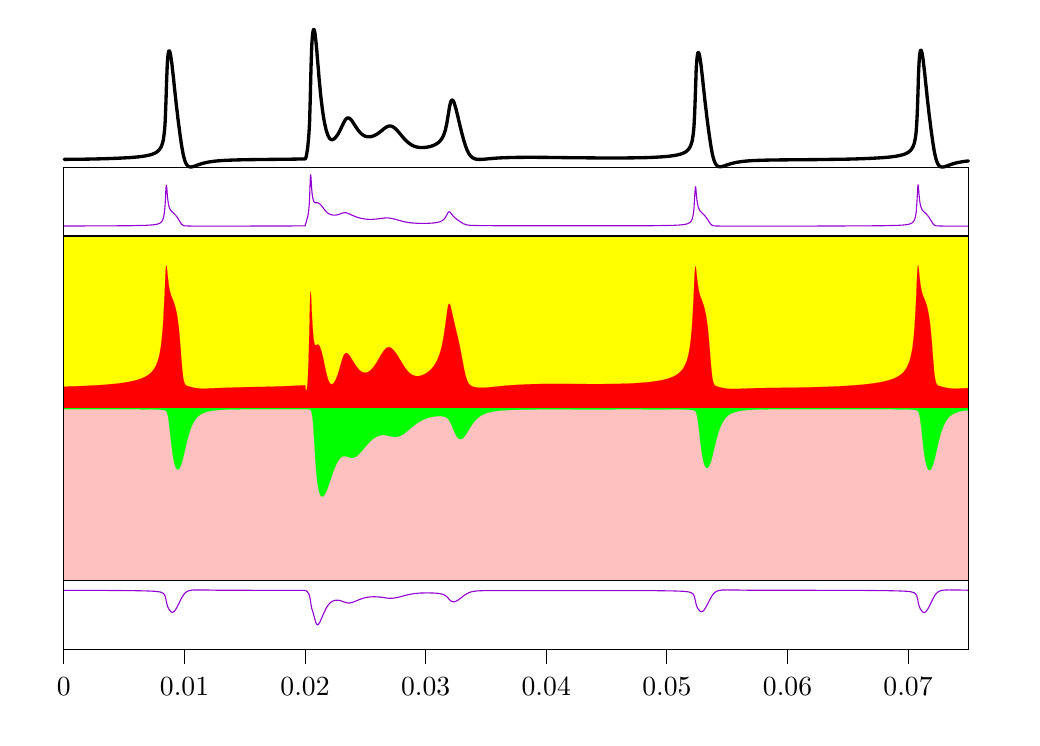
\begin{tikzpicture}[gnuplot]
%% generated with GNUPLOT 5.2p8 (Lua 5.3; terminal rev. Nov 2018, script rev. 108)
%% Wed Feb  3 22:37:26 2021
\path (0.000,0.000) rectangle (12.500,8.750);
\gpcolor{rgb color={0.000,0.000,0.000}}
\gpsetlinetype{gp lt border}
\gpsetdashtype{gp dt solid}
\gpsetlinewidth{3.00}
\draw[gp path] (0.464,7.097)--(0.468,7.097)--(0.471,7.097)--(0.475,7.097)--(0.479,7.097)%
  --(0.483,7.097)--(0.487,7.097)--(0.491,7.097)--(0.494,7.097)--(0.498,7.097)--(0.502,7.097)%
  --(0.506,7.097)--(0.510,7.097)--(0.514,7.097)--(0.517,7.098)--(0.521,7.098)--(0.525,7.098)%
  --(0.529,7.098)--(0.533,7.098)--(0.537,7.098)--(0.540,7.098)--(0.544,7.098)--(0.548,7.098)%
  --(0.552,7.098)--(0.556,7.098)--(0.560,7.098)--(0.563,7.098)--(0.567,7.098)--(0.571,7.098)%
  --(0.575,7.098)--(0.579,7.098)--(0.583,7.098)--(0.586,7.098)--(0.590,7.098)--(0.594,7.098)%
  --(0.598,7.099)--(0.602,7.099)--(0.606,7.099)--(0.609,7.099)--(0.613,7.099)--(0.617,7.099)%
  --(0.621,7.099)--(0.625,7.099)--(0.628,7.099)--(0.632,7.099)--(0.636,7.099)--(0.640,7.099)%
  --(0.644,7.099)--(0.648,7.099)--(0.651,7.099)--(0.655,7.099)--(0.659,7.099)--(0.663,7.099)%
  --(0.667,7.100)--(0.671,7.100)--(0.674,7.100)--(0.678,7.100)--(0.682,7.100)--(0.686,7.100)%
  --(0.690,7.100)--(0.694,7.100)--(0.697,7.100)--(0.701,7.100)--(0.705,7.100)--(0.709,7.100)%
  --(0.713,7.100)--(0.717,7.100)--(0.720,7.100)--(0.724,7.100)--(0.728,7.100)--(0.732,7.101)%
  --(0.736,7.101)--(0.740,7.101)--(0.743,7.101)--(0.747,7.101)--(0.751,7.101)--(0.755,7.101)%
  --(0.759,7.101)--(0.762,7.101)--(0.766,7.101)--(0.770,7.101)--(0.774,7.101)--(0.778,7.101)%
  --(0.782,7.101)--(0.785,7.102)--(0.789,7.102)--(0.793,7.102)--(0.797,7.102)--(0.801,7.102)%
  --(0.805,7.102)--(0.808,7.102)--(0.812,7.102)--(0.816,7.102)--(0.820,7.102)--(0.824,7.102)%
  --(0.828,7.102)--(0.831,7.102)--(0.835,7.102)--(0.839,7.103)--(0.843,7.103)--(0.847,7.103)%
  --(0.851,7.103)--(0.854,7.103)--(0.858,7.103)--(0.862,7.103)--(0.866,7.103)--(0.870,7.103)%
  --(0.874,7.103)--(0.877,7.103)--(0.881,7.103)--(0.885,7.104)--(0.889,7.104)--(0.893,7.104)%
  --(0.897,7.104)--(0.900,7.104)--(0.904,7.104)--(0.908,7.104)--(0.912,7.104)--(0.916,7.104)%
  --(0.919,7.104)--(0.923,7.105)--(0.927,7.105)--(0.931,7.105)--(0.935,7.105)--(0.939,7.105)%
  --(0.942,7.105)--(0.946,7.105)--(0.950,7.105)--(0.954,7.105)--(0.958,7.105)--(0.962,7.106)%
  --(0.965,7.106)--(0.969,7.106)--(0.973,7.106)--(0.977,7.106)--(0.981,7.106)--(0.985,7.106)%
  --(0.988,7.106)--(0.992,7.106)--(0.996,7.106)--(1.000,7.107)--(1.004,7.107)--(1.008,7.107)%
  --(1.011,7.107)--(1.015,7.107)--(1.019,7.107)--(1.023,7.107)--(1.027,7.107)--(1.031,7.108)%
  --(1.034,7.108)--(1.038,7.108)--(1.042,7.108)--(1.046,7.108)--(1.050,7.108)--(1.053,7.108)%
  --(1.057,7.108)--(1.061,7.109)--(1.065,7.109)--(1.069,7.109)--(1.073,7.109)--(1.076,7.109)%
  --(1.080,7.109)--(1.084,7.109)--(1.088,7.110)--(1.092,7.110)--(1.096,7.110)--(1.099,7.110)%
  --(1.103,7.110)--(1.107,7.110)--(1.111,7.110)--(1.115,7.111)--(1.119,7.111)--(1.122,7.111)%
  --(1.126,7.111)--(1.130,7.111)--(1.134,7.111)--(1.138,7.112)--(1.142,7.112)--(1.145,7.112)%
  --(1.149,7.112)--(1.153,7.112)--(1.157,7.112)--(1.161,7.113)--(1.165,7.113)--(1.168,7.113)%
  --(1.172,7.113)--(1.176,7.113)--(1.180,7.113)--(1.184,7.114)--(1.188,7.114)--(1.191,7.114)%
  --(1.195,7.114)--(1.199,7.114)--(1.203,7.115)--(1.207,7.115)--(1.210,7.115)--(1.214,7.115)%
  --(1.218,7.115)--(1.222,7.116)--(1.226,7.116)--(1.230,7.116)--(1.233,7.116)--(1.237,7.116)%
  --(1.241,7.117)--(1.245,7.117)--(1.249,7.117)--(1.253,7.117)--(1.256,7.117)--(1.260,7.118)%
  --(1.264,7.118)--(1.268,7.118)--(1.272,7.118)--(1.276,7.119)--(1.279,7.119)--(1.283,7.119)%
  --(1.287,7.119)--(1.291,7.120)--(1.295,7.120)--(1.299,7.120)--(1.302,7.120)--(1.306,7.121)%
  --(1.310,7.121)--(1.314,7.121)--(1.318,7.122)--(1.322,7.122)--(1.325,7.122)--(1.329,7.122)%
  --(1.333,7.123)--(1.337,7.123)--(1.341,7.123)--(1.344,7.124)--(1.348,7.124)--(1.352,7.124)%
  --(1.356,7.125)--(1.360,7.125)--(1.364,7.125)--(1.367,7.126)--(1.371,7.126)--(1.375,7.126)%
  --(1.379,7.127)--(1.383,7.127)--(1.387,7.127)--(1.390,7.128)--(1.394,7.128)--(1.398,7.129)%
  --(1.402,7.129)--(1.406,7.129)--(1.410,7.130)--(1.413,7.130)--(1.417,7.131)--(1.421,7.131)%
  --(1.425,7.132)--(1.429,7.132)--(1.433,7.133)--(1.436,7.133)--(1.440,7.133)--(1.444,7.134)%
  --(1.448,7.134)--(1.452,7.135)--(1.456,7.135)--(1.459,7.136)--(1.463,7.137)--(1.467,7.137)%
  --(1.471,7.138)--(1.475,7.138)--(1.479,7.139)--(1.482,7.140)--(1.486,7.140)--(1.490,7.141)%
  --(1.494,7.141)--(1.498,7.142)--(1.501,7.143)--(1.505,7.144)--(1.509,7.144)--(1.513,7.145)%
  --(1.517,7.146)--(1.521,7.147)--(1.524,7.147)--(1.528,7.148)--(1.532,7.149)--(1.536,7.150)%
  --(1.540,7.151)--(1.544,7.152)--(1.547,7.153)--(1.551,7.154)--(1.555,7.155)--(1.559,7.156)%
  --(1.563,7.157)--(1.567,7.158)--(1.570,7.159)--(1.574,7.160)--(1.578,7.162)--(1.582,7.163)%
  --(1.586,7.164)--(1.590,7.166)--(1.593,7.167)--(1.597,7.169)--(1.601,7.170)--(1.605,7.172)%
  --(1.609,7.174)--(1.613,7.176)--(1.616,7.177)--(1.620,7.179)--(1.624,7.182)--(1.628,7.184)%
  --(1.632,7.186)--(1.636,7.188)--(1.639,7.191)--(1.643,7.194)--(1.647,7.197)--(1.651,7.200)%
  --(1.655,7.203)--(1.658,7.206)--(1.662,7.210)--(1.666,7.214)--(1.670,7.218)--(1.674,7.223)%
  --(1.678,7.228)--(1.681,7.233)--(1.685,7.239)--(1.689,7.246)--(1.693,7.253)--(1.697,7.261)%
  --(1.701,7.269)--(1.704,7.279)--(1.708,7.290)--(1.712,7.303)--(1.716,7.317)--(1.720,7.334)%
  --(1.724,7.353)--(1.727,7.376)--(1.731,7.403)--(1.735,7.436)--(1.739,7.477)--(1.743,7.528)%
  --(1.747,7.592)--(1.750,7.673)--(1.754,7.774)--(1.758,7.891)--(1.762,8.016)--(1.766,8.133)%
  --(1.770,8.231)--(1.773,8.309)--(1.777,8.368)--(1.781,8.411)--(1.785,8.442)--(1.789,8.462)%
  --(1.792,8.473)--(1.796,8.477)--(1.800,8.475)--(1.804,8.468)--(1.808,8.455)--(1.812,8.439)%
  --(1.815,8.419)--(1.819,8.396)--(1.823,8.371)--(1.827,8.343)--(1.831,8.313)--(1.835,8.281)%
  --(1.838,8.248)--(1.842,8.214)--(1.846,8.179)--(1.850,8.143)--(1.854,8.107)--(1.858,8.071)%
  --(1.861,8.035)--(1.865,7.998)--(1.869,7.962)--(1.873,7.926)--(1.877,7.891)--(1.881,7.856)%
  --(1.884,7.821)--(1.888,7.787)--(1.892,7.753)--(1.896,7.720)--(1.900,7.688)--(1.904,7.656)%
  --(1.907,7.624)--(1.911,7.594)--(1.915,7.563)--(1.919,7.533)--(1.923,7.504)--(1.927,7.475)%
  --(1.930,7.446)--(1.934,7.418)--(1.938,7.391)--(1.942,7.364)--(1.946,7.337)--(1.949,7.311)%
  --(1.953,7.286)--(1.957,7.262)--(1.961,7.239)--(1.965,7.217)--(1.969,7.196)--(1.972,7.176)%
  --(1.976,7.158)--(1.980,7.140)--(1.984,7.124)--(1.988,7.110)--(1.992,7.096)--(1.995,7.084)%
  --(1.999,7.073)--(2.003,7.063)--(2.007,7.054)--(2.011,7.046)--(2.015,7.039)--(2.018,7.033)%
  --(2.022,7.027)--(2.026,7.022)--(2.030,7.018)--(2.034,7.015)--(2.038,7.012)--(2.041,7.009)%
  --(2.045,7.007)--(2.049,7.005)--(2.053,7.004)--(2.057,7.003)--(2.061,7.002)--(2.064,7.002)%
  --(2.068,7.001)--(2.072,7.001)--(2.076,7.001)--(2.080,7.002)--(2.083,7.002)--(2.087,7.003)%
  --(2.091,7.004)--(2.095,7.005)--(2.099,7.006)--(2.103,7.007)--(2.106,7.008)--(2.110,7.009)%
  --(2.114,7.010)--(2.118,7.011)--(2.122,7.013)--(2.126,7.014)--(2.129,7.015)--(2.133,7.017)%
  --(2.137,7.018)--(2.141,7.019)--(2.145,7.021)--(2.149,7.022)--(2.152,7.024)--(2.156,7.025)%
  --(2.160,7.026)--(2.164,7.028)--(2.168,7.029)--(2.172,7.030)--(2.175,7.032)--(2.179,7.033)%
  --(2.183,7.034)--(2.187,7.035)--(2.191,7.037)--(2.195,7.038)--(2.198,7.039)--(2.202,7.040)%
  --(2.206,7.042)--(2.210,7.043)--(2.214,7.044)--(2.218,7.045)--(2.221,7.046)--(2.225,7.047)%
  --(2.229,7.048)--(2.233,7.049)--(2.237,7.050)--(2.240,7.051)--(2.244,7.052)--(2.248,7.053)%
  --(2.252,7.054)--(2.256,7.055)--(2.260,7.056)--(2.263,7.056)--(2.267,7.057)--(2.271,7.058)%
  --(2.275,7.059)--(2.279,7.060)--(2.283,7.060)--(2.286,7.061)--(2.290,7.062)--(2.294,7.063)%
  --(2.298,7.063)--(2.302,7.064)--(2.306,7.065)--(2.309,7.065)--(2.313,7.066)--(2.317,7.067)%
  --(2.321,7.067)--(2.325,7.068)--(2.329,7.068)--(2.332,7.069)--(2.336,7.069)--(2.340,7.070)%
  --(2.344,7.070)--(2.348,7.071)--(2.352,7.071)--(2.355,7.072)--(2.359,7.072)--(2.363,7.073)%
  --(2.367,7.073)--(2.371,7.074)--(2.375,7.074)--(2.378,7.075)--(2.382,7.075)--(2.386,7.076)%
  --(2.390,7.076)--(2.394,7.076)--(2.397,7.077)--(2.401,7.077)--(2.405,7.077)--(2.409,7.078)%
  --(2.413,7.078)--(2.417,7.078)--(2.420,7.079)--(2.424,7.079)--(2.428,7.079)--(2.432,7.080)%
  --(2.436,7.080)--(2.440,7.080)--(2.443,7.081)--(2.447,7.081)--(2.451,7.081)--(2.455,7.082)%
  --(2.459,7.082)--(2.463,7.082)--(2.466,7.082)--(2.470,7.083)--(2.474,7.083)--(2.478,7.083)%
  --(2.482,7.083)--(2.486,7.084)--(2.489,7.084)--(2.493,7.084)--(2.497,7.084)--(2.501,7.084)%
  --(2.505,7.085)--(2.509,7.085)--(2.512,7.085)--(2.516,7.085)--(2.520,7.085)--(2.524,7.086)%
  --(2.528,7.086)--(2.531,7.086)--(2.535,7.086)--(2.539,7.086)--(2.543,7.087)--(2.547,7.087)%
  --(2.551,7.087)--(2.554,7.087)--(2.558,7.087)--(2.562,7.087)--(2.566,7.087)--(2.570,7.088)%
  --(2.574,7.088)--(2.577,7.088)--(2.581,7.088)--(2.585,7.088)--(2.589,7.088)--(2.593,7.088)%
  --(2.597,7.089)--(2.600,7.089)--(2.604,7.089)--(2.608,7.089)--(2.612,7.089)--(2.616,7.089)%
  --(2.620,7.089)--(2.623,7.089)--(2.627,7.090)--(2.631,7.090)--(2.635,7.090)--(2.639,7.090)%
  --(2.643,7.090)--(2.646,7.090)--(2.650,7.090)--(2.654,7.090)--(2.658,7.090)--(2.662,7.091)%
  --(2.666,7.091)--(2.669,7.091)--(2.673,7.091)--(2.677,7.091)--(2.681,7.091)--(2.685,7.091)%
  --(2.688,7.091)--(2.692,7.091)--(2.696,7.091)--(2.700,7.091)--(2.704,7.092)--(2.708,7.092)%
  --(2.711,7.092)--(2.715,7.092)--(2.719,7.092)--(2.723,7.092)--(2.727,7.092)--(2.731,7.092)%
  --(2.734,7.092)--(2.738,7.092)--(2.742,7.092)--(2.746,7.092)--(2.750,7.092)--(2.754,7.093)%
  --(2.757,7.093)--(2.761,7.093)--(2.765,7.093)--(2.769,7.093)--(2.773,7.093)--(2.777,7.093)%
  --(2.780,7.093)--(2.784,7.093)--(2.788,7.093)--(2.792,7.093)--(2.796,7.093)--(2.800,7.093)%
  --(2.803,7.093)--(2.807,7.093)--(2.811,7.093)--(2.815,7.094)--(2.819,7.094)--(2.822,7.094)%
  --(2.826,7.094)--(2.830,7.094)--(2.834,7.094)--(2.838,7.094)--(2.842,7.094)--(2.845,7.094)%
  --(2.849,7.094)--(2.853,7.094)--(2.857,7.094)--(2.861,7.094)--(2.865,7.094)--(2.868,7.094)%
  --(2.872,7.094)--(2.876,7.094)--(2.880,7.094)--(2.884,7.094)--(2.888,7.095)--(2.891,7.095)%
  --(2.895,7.095)--(2.899,7.095)--(2.903,7.095)--(2.907,7.095)--(2.911,7.095)--(2.914,7.095)%
  --(2.918,7.095)--(2.922,7.095)--(2.926,7.095)--(2.930,7.095)--(2.934,7.095)--(2.937,7.095)%
  --(2.941,7.095)--(2.945,7.095)--(2.949,7.095)--(2.953,7.095)--(2.957,7.095)--(2.960,7.095)%
  --(2.964,7.095)--(2.968,7.095)--(2.972,7.096)--(2.976,7.096)--(2.979,7.096)--(2.983,7.096)%
  --(2.987,7.096)--(2.991,7.096)--(2.995,7.096)--(2.999,7.096)--(3.002,7.096)--(3.006,7.096)%
  --(3.010,7.096)--(3.014,7.096)--(3.018,7.096)--(3.022,7.096)--(3.025,7.096)--(3.029,7.096)%
  --(3.033,7.096)--(3.037,7.096)--(3.041,7.096)--(3.045,7.096)--(3.048,7.096)--(3.052,7.096)%
  --(3.056,7.096)--(3.060,7.097)--(3.064,7.097)--(3.068,7.097)--(3.071,7.097)--(3.075,7.097)%
  --(3.079,7.097)--(3.083,7.097)--(3.087,7.097)--(3.091,7.097)--(3.094,7.097)--(3.098,7.097)%
  --(3.102,7.097)--(3.106,7.097)--(3.110,7.097)--(3.113,7.097)--(3.117,7.097)--(3.121,7.097)%
  --(3.125,7.097)--(3.129,7.097)--(3.133,7.097)--(3.136,7.097)--(3.140,7.097)--(3.144,7.097)%
  --(3.148,7.098)--(3.152,7.098)--(3.156,7.098)--(3.159,7.098)--(3.163,7.098)--(3.167,7.098)%
  --(3.171,7.098)--(3.175,7.098)--(3.179,7.098)--(3.182,7.098)--(3.186,7.098)--(3.190,7.098)%
  --(3.194,7.098)--(3.198,7.098)--(3.202,7.098)--(3.205,7.098)--(3.209,7.098)--(3.213,7.098)%
  --(3.217,7.098)--(3.221,7.098)--(3.225,7.099)--(3.228,7.099)--(3.232,7.099)--(3.236,7.099)%
  --(3.240,7.099)--(3.244,7.099)--(3.248,7.099)--(3.251,7.099)--(3.255,7.099)--(3.259,7.099)%
  --(3.263,7.099)--(3.267,7.099)--(3.270,7.099)--(3.274,7.099)--(3.278,7.099)--(3.282,7.099)%
  --(3.286,7.099)--(3.290,7.099)--(3.293,7.099)--(3.297,7.100)--(3.301,7.100)--(3.305,7.100)%
  --(3.309,7.100)--(3.313,7.100)--(3.316,7.100)--(3.320,7.100)--(3.324,7.100)--(3.328,7.100)%
  --(3.332,7.100)--(3.336,7.100)--(3.339,7.100)--(3.343,7.100)--(3.347,7.100)--(3.351,7.100)%
  --(3.355,7.100)--(3.359,7.101)--(3.362,7.101)--(3.366,7.101)--(3.370,7.101)--(3.374,7.101)%
  --(3.378,7.101)--(3.382,7.101)--(3.385,7.101)--(3.389,7.101)--(3.393,7.101)--(3.397,7.101)%
  --(3.401,7.101)--(3.405,7.101)--(3.408,7.101)--(3.412,7.101)--(3.416,7.102)--(3.420,7.102)%
  --(3.424,7.102)--(3.427,7.102)--(3.431,7.102)--(3.435,7.102)--(3.439,7.102)--(3.443,7.102)%
  --(3.447,7.102)--(3.450,7.102)--(3.454,7.102)--(3.458,7.102)--(3.462,7.102)--(3.466,7.103)%
  --(3.470,7.103)--(3.473,7.103)--(3.477,7.103)--(3.481,7.103)--(3.485,7.103)--(3.489,7.103)%
  --(3.493,7.103)--(3.496,7.103)--(3.500,7.103)--(3.504,7.103)--(3.508,7.103)--(3.512,7.104)%
  --(3.516,7.104)--(3.519,7.104)--(3.523,7.104)--(3.527,7.106)--(3.531,7.114)--(3.535,7.125)%
  --(3.539,7.140)--(3.542,7.159)--(3.546,7.180)--(3.550,7.205)--(3.554,7.232)--(3.558,7.263)%
  --(3.561,7.298)--(3.565,7.338)--(3.569,7.385)--(3.573,7.440)--(3.577,7.508)--(3.581,7.593)%
  --(3.584,7.702)--(3.588,7.841)--(3.592,8.003)--(3.596,8.169)--(3.600,8.314)--(3.604,8.432)%
  --(3.607,8.523)--(3.611,8.595)--(3.615,8.649)--(3.619,8.689)--(3.623,8.718)--(3.627,8.737)%
  --(3.630,8.747)--(3.634,8.749)--(3.638,8.744)--(3.642,8.732)--(3.646,8.714)--(3.650,8.691)%
  --(3.653,8.662)--(3.657,8.630)--(3.661,8.593)--(3.665,8.553)--(3.669,8.511)--(3.673,8.467)%
  --(3.676,8.422)--(3.680,8.376)--(3.684,8.329)--(3.688,8.283)--(3.692,8.237)--(3.696,8.192)%
  --(3.699,8.147)--(3.703,8.104)--(3.707,8.061)--(3.711,8.020)--(3.715,7.981)--(3.718,7.943)%
  --(3.722,7.906)--(3.726,7.871)--(3.730,7.837)--(3.734,7.805)--(3.738,7.774)--(3.741,7.744)%
  --(3.745,7.716)--(3.749,7.689)--(3.753,7.663)--(3.757,7.639)--(3.761,7.616)--(3.764,7.594)%
  --(3.768,7.573)--(3.772,7.553)--(3.776,7.534)--(3.780,7.517)--(3.784,7.500)--(3.787,7.484)%
  --(3.791,7.469)--(3.795,7.456)--(3.799,7.443)--(3.803,7.431)--(3.807,7.420)--(3.810,7.410)%
  --(3.814,7.401)--(3.818,7.392)--(3.822,7.385)--(3.826,7.378)--(3.830,7.372)--(3.833,7.367)%
  --(3.837,7.362)--(3.841,7.358)--(3.845,7.355)--(3.849,7.352)--(3.852,7.350)--(3.856,7.349)%
  --(3.860,7.348)--(3.864,7.348)--(3.868,7.348)--(3.872,7.349)--(3.875,7.350)--(3.879,7.351)%
  --(3.883,7.353)--(3.887,7.355)--(3.891,7.358)--(3.895,7.361)--(3.898,7.364)--(3.902,7.368)%
  --(3.906,7.372)--(3.910,7.376)--(3.914,7.380)--(3.918,7.385)--(3.921,7.390)--(3.925,7.395)%
  --(3.929,7.401)--(3.933,7.406)--(3.937,7.412)--(3.941,7.418)--(3.944,7.425)--(3.948,7.431)%
  --(3.952,7.438)--(3.956,7.445)--(3.960,7.452)--(3.964,7.460)--(3.967,7.467)--(3.971,7.475)%
  --(3.975,7.483)--(3.979,7.491)--(3.983,7.499)--(3.987,7.507)--(3.990,7.515)--(3.994,7.523)%
  --(3.998,7.531)--(4.002,7.539)--(4.006,7.547)--(4.009,7.555)--(4.013,7.563)--(4.017,7.570)%
  --(4.021,7.577)--(4.025,7.584)--(4.029,7.590)--(4.032,7.596)--(4.036,7.602)--(4.040,7.606)%
  --(4.044,7.611)--(4.048,7.614)--(4.052,7.617)--(4.055,7.620)--(4.059,7.622)--(4.063,7.623)%
  --(4.067,7.624)--(4.071,7.624)--(4.075,7.623)--(4.078,7.622)--(4.082,7.621)--(4.086,7.619)%
  --(4.090,7.616)--(4.094,7.613)--(4.098,7.610)--(4.101,7.606)--(4.105,7.602)--(4.109,7.597)%
  --(4.113,7.593)--(4.117,7.588)--(4.121,7.582)--(4.124,7.577)--(4.128,7.571)--(4.132,7.566)%
  --(4.136,7.560)--(4.140,7.554)--(4.143,7.548)--(4.147,7.542)--(4.151,7.536)--(4.155,7.530)%
  --(4.159,7.524)--(4.163,7.518)--(4.166,7.512)--(4.170,7.507)--(4.174,7.501)--(4.178,7.495)%
  --(4.182,7.490)--(4.186,7.484)--(4.189,7.479)--(4.193,7.474)--(4.197,7.468)--(4.201,7.464)%
  --(4.205,7.459)--(4.209,7.454)--(4.212,7.449)--(4.216,7.445)--(4.220,7.441)--(4.224,7.437)%
  --(4.228,7.433)--(4.232,7.429)--(4.235,7.425)--(4.239,7.422)--(4.243,7.419)--(4.247,7.416)%
  --(4.251,7.413)--(4.255,7.410)--(4.258,7.407)--(4.262,7.405)--(4.266,7.402)--(4.270,7.400)%
  --(4.274,7.398)--(4.278,7.396)--(4.281,7.394)--(4.285,7.393)--(4.289,7.391)--(4.293,7.390)%
  --(4.297,7.389)--(4.300,7.388)--(4.304,7.387)--(4.308,7.386)--(4.312,7.385)--(4.316,7.385)%
  --(4.320,7.384)--(4.323,7.384)--(4.327,7.384)--(4.331,7.384)--(4.335,7.384)--(4.339,7.384)%
  --(4.343,7.384)--(4.346,7.385)--(4.350,7.385)--(4.354,7.386)--(4.358,7.386)--(4.362,7.387)%
  --(4.366,7.388)--(4.369,7.389)--(4.373,7.390)--(4.377,7.391)--(4.381,7.392)--(4.385,7.393)%
  --(4.389,7.395)--(4.392,7.396)--(4.396,7.398)--(4.400,7.399)--(4.404,7.401)--(4.408,7.403)%
  --(4.412,7.405)--(4.415,7.407)--(4.419,7.409)--(4.423,7.411)--(4.427,7.413)--(4.431,7.415)%
  --(4.435,7.417)--(4.438,7.420)--(4.442,7.422)--(4.446,7.425)--(4.450,7.427)--(4.454,7.430)%
  --(4.457,7.433)--(4.461,7.435)--(4.465,7.438)--(4.469,7.441)--(4.473,7.444)--(4.477,7.447)%
  --(4.480,7.450)--(4.484,7.453)--(4.488,7.456)--(4.492,7.459)--(4.496,7.462)--(4.500,7.465)%
  --(4.503,7.468)--(4.507,7.472)--(4.511,7.475)--(4.515,7.478)--(4.519,7.481)--(4.523,7.484)%
  --(4.526,7.487)--(4.530,7.490)--(4.534,7.493)--(4.538,7.495)--(4.542,7.498)--(4.546,7.501)%
  --(4.549,7.503)--(4.553,7.505)--(4.557,7.508)--(4.561,7.510)--(4.565,7.512)--(4.569,7.513)%
  --(4.572,7.515)--(4.576,7.517)--(4.580,7.518)--(4.584,7.519)--(4.588,7.520)--(4.591,7.520)%
  --(4.595,7.521)--(4.599,7.521)--(4.603,7.521)--(4.607,7.521)--(4.611,7.520)--(4.614,7.520)%
  --(4.618,7.519)--(4.622,7.518)--(4.626,7.516)--(4.630,7.515)--(4.634,7.513)--(4.637,7.511)%
  --(4.641,7.509)--(4.645,7.506)--(4.649,7.504)--(4.653,7.501)--(4.657,7.498)--(4.660,7.495)%
  --(4.664,7.492)--(4.668,7.489)--(4.672,7.485)--(4.676,7.482)--(4.680,7.478)--(4.683,7.474)%
  --(4.687,7.470)--(4.691,7.466)--(4.695,7.462)--(4.699,7.458)--(4.703,7.453)--(4.706,7.449)%
  --(4.710,7.445)--(4.714,7.440)--(4.718,7.436)--(4.722,7.431)--(4.726,7.427)--(4.729,7.422)%
  --(4.733,7.417)--(4.737,7.413)--(4.741,7.408)--(4.745,7.404)--(4.748,7.399)--(4.752,7.395)%
  --(4.756,7.390)--(4.760,7.386)--(4.764,7.381)--(4.768,7.377)--(4.771,7.372)--(4.775,7.368)%
  --(4.779,7.364)--(4.783,7.359)--(4.787,7.355)--(4.791,7.351)--(4.794,7.347)--(4.798,7.343)%
  --(4.802,7.339)--(4.806,7.336)--(4.810,7.332)--(4.814,7.328)--(4.817,7.325)--(4.821,7.321)%
  --(4.825,7.318)--(4.829,7.314)--(4.833,7.311)--(4.837,7.308)--(4.840,7.305)--(4.844,7.302)%
  --(4.848,7.299)--(4.852,7.296)--(4.856,7.294)--(4.860,7.291)--(4.863,7.288)--(4.867,7.286)%
  --(4.871,7.284)--(4.875,7.281)--(4.879,7.279)--(4.882,7.277)--(4.886,7.275)--(4.890,7.273)%
  --(4.894,7.271)--(4.898,7.270)--(4.902,7.268)--(4.905,7.266)--(4.909,7.265)--(4.913,7.263)%
  --(4.917,7.262)--(4.921,7.261)--(4.925,7.260)--(4.928,7.258)--(4.932,7.257)--(4.936,7.256)%
  --(4.940,7.255)--(4.944,7.254)--(4.948,7.254)--(4.951,7.253)--(4.955,7.252)--(4.959,7.251)%
  --(4.963,7.251)--(4.967,7.250)--(4.971,7.250)--(4.974,7.249)--(4.978,7.249)--(4.982,7.249)%
  --(4.986,7.248)--(4.990,7.248)--(4.994,7.248)--(4.997,7.248)--(5.001,7.248)--(5.005,7.248)%
  --(5.009,7.248)--(5.013,7.248)--(5.017,7.248)--(5.020,7.248)--(5.024,7.248)--(5.028,7.248)%
  --(5.032,7.248)--(5.036,7.249)--(5.039,7.249)--(5.043,7.249)--(5.047,7.250)--(5.051,7.250)%
  --(5.055,7.250)--(5.059,7.251)--(5.062,7.251)--(5.066,7.252)--(5.070,7.253)--(5.074,7.253)%
  --(5.078,7.254)--(5.082,7.254)--(5.085,7.255)--(5.089,7.256)--(5.093,7.257)--(5.097,7.258)%
  --(5.101,7.258)--(5.105,7.259)--(5.108,7.260)--(5.112,7.261)--(5.116,7.262)--(5.120,7.263)%
  --(5.124,7.265)--(5.128,7.266)--(5.131,7.267)--(5.135,7.268)--(5.139,7.270)--(5.143,7.271)%
  --(5.147,7.272)--(5.151,7.274)--(5.154,7.275)--(5.158,7.277)--(5.162,7.279)--(5.166,7.280)%
  --(5.170,7.282)--(5.173,7.284)--(5.177,7.286)--(5.181,7.288)--(5.185,7.290)--(5.189,7.293)%
  --(5.193,7.295)--(5.196,7.297)--(5.200,7.300)--(5.204,7.303)--(5.208,7.305)--(5.212,7.308)%
  --(5.216,7.311)--(5.219,7.315)--(5.223,7.318)--(5.227,7.322)--(5.231,7.325)--(5.235,7.329)%
  --(5.239,7.333)--(5.242,7.338)--(5.246,7.343)--(5.250,7.348)--(5.254,7.353)--(5.258,7.359)%
  --(5.262,7.365)--(5.265,7.371)--(5.269,7.378)--(5.273,7.385)--(5.277,7.393)--(5.281,7.402)%
  --(5.285,7.411)--(5.288,7.421)--(5.292,7.432)--(5.296,7.443)--(5.300,7.456)--(5.304,7.469)%
  --(5.308,7.484)--(5.311,7.500)--(5.315,7.517)--(5.319,7.535)--(5.323,7.555)--(5.327,7.575)%
  --(5.330,7.598)--(5.334,7.621)--(5.338,7.644)--(5.342,7.669)--(5.346,7.693)--(5.350,7.717)%
  --(5.353,7.740)--(5.357,7.761)--(5.361,7.781)--(5.365,7.798)--(5.369,7.813)--(5.373,7.825)%
  --(5.376,7.835)--(5.380,7.843)--(5.384,7.848)--(5.388,7.851)--(5.392,7.851)--(5.396,7.850)%
  --(5.399,7.846)--(5.403,7.841)--(5.407,7.835)--(5.411,7.827)--(5.415,7.818)--(5.419,7.808)%
  --(5.422,7.796)--(5.426,7.784)--(5.430,7.771)--(5.434,7.758)--(5.438,7.744)--(5.442,7.729)%
  --(5.445,7.714)--(5.449,7.699)--(5.453,7.683)--(5.457,7.667)--(5.461,7.651)--(5.465,7.635)%
  --(5.468,7.619)--(5.472,7.603)--(5.476,7.586)--(5.480,7.570)--(5.484,7.554)--(5.487,7.538)%
  --(5.491,7.522)--(5.495,7.506)--(5.499,7.490)--(5.503,7.475)--(5.507,7.459)--(5.510,7.444)%
  --(5.514,7.429)--(5.518,7.414)--(5.522,7.400)--(5.526,7.385)--(5.530,7.371)--(5.533,7.357)%
  --(5.537,7.344)--(5.541,7.331)--(5.545,7.318)--(5.549,7.305)--(5.553,7.293)--(5.556,7.281)%
  --(5.560,7.270)--(5.564,7.259)--(5.568,7.248)--(5.572,7.238)--(5.576,7.229)--(5.579,7.219)%
  --(5.583,7.211)--(5.587,7.202)--(5.591,7.194)--(5.595,7.187)--(5.599,7.180)--(5.602,7.173)%
  --(5.606,7.167)--(5.610,7.161)--(5.614,7.156)--(5.618,7.150)--(5.621,7.146)--(5.625,7.141)%
  --(5.629,7.137)--(5.633,7.133)--(5.637,7.129)--(5.641,7.126)--(5.644,7.123)--(5.648,7.120)%
  --(5.652,7.118)--(5.656,7.115)--(5.660,7.113)--(5.664,7.111)--(5.667,7.109)--(5.671,7.108)%
  --(5.675,7.106)--(5.679,7.105)--(5.683,7.104)--(5.687,7.102)--(5.690,7.101)--(5.694,7.101)%
  --(5.698,7.100)--(5.702,7.099)--(5.706,7.099)--(5.710,7.098)--(5.713,7.098)--(5.717,7.097)%
  --(5.721,7.097)--(5.725,7.097)--(5.729,7.097)--(5.733,7.097)--(5.736,7.097)--(5.740,7.097)%
  --(5.744,7.097)--(5.748,7.097)--(5.752,7.097)--(5.756,7.097)--(5.759,7.097)--(5.763,7.097)%
  --(5.767,7.097)--(5.771,7.098)--(5.775,7.098)--(5.778,7.098)--(5.782,7.098)--(5.786,7.099)%
  --(5.790,7.099)--(5.794,7.099)--(5.798,7.100)--(5.801,7.100)--(5.805,7.100)--(5.809,7.101)%
  --(5.813,7.101)--(5.817,7.101)--(5.821,7.102)--(5.824,7.102)--(5.828,7.102)--(5.832,7.103)%
  --(5.836,7.103)--(5.840,7.103)--(5.844,7.104)--(5.847,7.104)--(5.851,7.105)--(5.855,7.105)%
  --(5.859,7.105)--(5.863,7.106)--(5.867,7.106)--(5.870,7.106)--(5.874,7.107)--(5.878,7.107)%
  --(5.882,7.107)--(5.886,7.108)--(5.890,7.108)--(5.893,7.108)--(5.897,7.109)--(5.901,7.109)%
  --(5.905,7.109)--(5.909,7.110)--(5.912,7.110)--(5.916,7.110)--(5.920,7.111)--(5.924,7.111)%
  --(5.928,7.111)--(5.932,7.111)--(5.935,7.112)--(5.939,7.112)--(5.943,7.112)--(5.947,7.113)%
  --(5.951,7.113)--(5.955,7.113)--(5.958,7.113)--(5.962,7.114)--(5.966,7.114)--(5.970,7.114)%
  --(5.974,7.114)--(5.978,7.115)--(5.981,7.115)--(5.985,7.115)--(5.989,7.115)--(5.993,7.115)%
  --(5.997,7.116)--(6.001,7.116)--(6.004,7.116)--(6.008,7.116)--(6.012,7.116)--(6.016,7.117)%
  --(6.020,7.117)--(6.024,7.117)--(6.027,7.117)--(6.031,7.117)--(6.035,7.118)--(6.039,7.118)%
  --(6.043,7.118)--(6.047,7.118)--(6.050,7.118)--(6.054,7.118)--(6.058,7.119)--(6.062,7.119)%
  --(6.066,7.119)--(6.069,7.119)--(6.073,7.119)--(6.077,7.119)--(6.081,7.119)--(6.085,7.120)%
  --(6.089,7.120)--(6.092,7.120)--(6.096,7.120)--(6.100,7.120)--(6.104,7.120)--(6.108,7.120)%
  --(6.112,7.120)--(6.115,7.121)--(6.119,7.121)--(6.123,7.121)--(6.127,7.121)--(6.131,7.121)%
  --(6.135,7.121)--(6.138,7.121)--(6.142,7.121)--(6.146,7.121)--(6.150,7.121)--(6.154,7.122)%
  --(6.158,7.122)--(6.161,7.122)--(6.165,7.122)--(6.169,7.122)--(6.173,7.122)--(6.177,7.122)%
  --(6.181,7.122)--(6.184,7.122)--(6.188,7.122)--(6.192,7.122)--(6.196,7.122)--(6.200,7.122)%
  --(6.204,7.122)--(6.207,7.123)--(6.211,7.123)--(6.215,7.123)--(6.219,7.123)--(6.223,7.123)%
  --(6.226,7.123)--(6.230,7.123)--(6.234,7.123)--(6.238,7.123)--(6.242,7.123)--(6.246,7.123)%
  --(6.249,7.123)--(6.253,7.123)--(6.257,7.123)--(6.261,7.123)--(6.265,7.123)--(6.269,7.123)%
  --(6.272,7.123)--(6.276,7.123)--(6.280,7.123)--(6.284,7.123)--(6.288,7.123)--(6.292,7.123)%
  --(6.295,7.123)--(6.299,7.123)--(6.303,7.124)--(6.307,7.124)--(6.311,7.124)--(6.315,7.124)%
  --(6.318,7.124)--(6.322,7.124)--(6.326,7.124)--(6.330,7.124)--(6.334,7.124)--(6.338,7.124)%
  --(6.341,7.124)--(6.345,7.124)--(6.349,7.124)--(6.353,7.124)--(6.357,7.124)--(6.360,7.124)%
  --(6.364,7.124)--(6.368,7.124)--(6.372,7.124)--(6.376,7.124)--(6.380,7.124)--(6.383,7.124)%
  --(6.387,7.124)--(6.391,7.124)--(6.395,7.124)--(6.399,7.124)--(6.403,7.124)--(6.406,7.124)%
  --(6.410,7.124)--(6.414,7.124)--(6.418,7.124)--(6.422,7.124)--(6.426,7.124)--(6.429,7.124)%
  --(6.433,7.124)--(6.437,7.124)--(6.441,7.124)--(6.445,7.124)--(6.449,7.124)--(6.452,7.124)%
  --(6.456,7.124)--(6.460,7.124)--(6.464,7.124)--(6.468,7.123)--(6.472,7.123)--(6.475,7.123)%
  --(6.479,7.123)--(6.483,7.123)--(6.487,7.123)--(6.491,7.123)--(6.495,7.123)--(6.498,7.123)%
  --(6.502,7.123)--(6.506,7.123)--(6.510,7.123)--(6.514,7.123)--(6.517,7.123)--(6.521,7.123)%
  --(6.525,7.123)--(6.529,7.123)--(6.533,7.123)--(6.537,7.123)--(6.540,7.123)--(6.544,7.123)%
  --(6.548,7.123)--(6.552,7.123)--(6.556,7.123)--(6.560,7.123)--(6.563,7.123)--(6.567,7.123)%
  --(6.571,7.123)--(6.575,7.123)--(6.579,7.123)--(6.583,7.123)--(6.586,7.123)--(6.590,7.123)%
  --(6.594,7.123)--(6.598,7.123)--(6.602,7.122)--(6.606,7.122)--(6.609,7.122)--(6.613,7.122)%
  --(6.617,7.122)--(6.621,7.122)--(6.625,7.122)--(6.629,7.122)--(6.632,7.122)--(6.636,7.122)%
  --(6.640,7.122)--(6.644,7.122)--(6.648,7.122)--(6.651,7.122)--(6.655,7.122)--(6.659,7.122)%
  --(6.663,7.122)--(6.667,7.122)--(6.671,7.122)--(6.674,7.122)--(6.678,7.122)--(6.682,7.122)%
  --(6.686,7.122)--(6.690,7.122)--(6.694,7.121)--(6.697,7.121)--(6.701,7.121)--(6.705,7.121)%
  --(6.709,7.121)--(6.713,7.121)--(6.717,7.121)--(6.720,7.121)--(6.724,7.121)--(6.728,7.121)%
  --(6.732,7.121)--(6.736,7.121)--(6.740,7.121)--(6.743,7.121)--(6.747,7.121)--(6.751,7.121)%
  --(6.755,7.121)--(6.759,7.121)--(6.763,7.121)--(6.766,7.121)--(6.770,7.121)--(6.774,7.121)%
  --(6.778,7.120)--(6.782,7.120)--(6.786,7.120)--(6.789,7.120)--(6.793,7.120)--(6.797,7.120)%
  --(6.801,7.120)--(6.805,7.120)--(6.808,7.120)--(6.812,7.120)--(6.816,7.120)--(6.820,7.120)%
  --(6.824,7.120)--(6.828,7.120)--(6.831,7.120)--(6.835,7.120)--(6.839,7.120)--(6.843,7.120)%
  --(6.847,7.120)--(6.851,7.120)--(6.854,7.119)--(6.858,7.119)--(6.862,7.119)--(6.866,7.119)%
  --(6.870,7.119)--(6.874,7.119)--(6.877,7.119)--(6.881,7.119)--(6.885,7.119)--(6.889,7.119)%
  --(6.893,7.119)--(6.897,7.119)--(6.900,7.119)--(6.904,7.119)--(6.908,7.119)--(6.912,7.119)%
  --(6.916,7.119)--(6.920,7.119)--(6.923,7.119)--(6.927,7.119)--(6.931,7.118)--(6.935,7.118)%
  --(6.939,7.118)--(6.942,7.118)--(6.946,7.118)--(6.950,7.118)--(6.954,7.118)--(6.958,7.118)%
  --(6.962,7.118)--(6.965,7.118)--(6.969,7.118)--(6.973,7.118)--(6.977,7.118)--(6.981,7.118)%
  --(6.985,7.118)--(6.988,7.118)--(6.992,7.118)--(6.996,7.118)--(7.000,7.118)--(7.004,7.118)%
  --(7.008,7.118)--(7.011,7.118)--(7.015,7.117)--(7.019,7.117)--(7.023,7.117)--(7.027,7.117)%
  --(7.031,7.117)--(7.034,7.117)--(7.038,7.117)--(7.042,7.117)--(7.046,7.117)--(7.050,7.117)%
  --(7.054,7.117)--(7.057,7.117)--(7.061,7.117)--(7.065,7.117)--(7.069,7.117)--(7.073,7.117)%
  --(7.077,7.117)--(7.080,7.117)--(7.084,7.117)--(7.088,7.117)--(7.092,7.117)--(7.096,7.117)%
  --(7.099,7.117)--(7.103,7.116)--(7.107,7.116)--(7.111,7.116)--(7.115,7.116)--(7.119,7.116)%
  --(7.122,7.116)--(7.126,7.116)--(7.130,7.116)--(7.134,7.116)--(7.138,7.116)--(7.142,7.116)%
  --(7.145,7.116)--(7.149,7.116)--(7.153,7.116)--(7.157,7.116)--(7.161,7.116)--(7.165,7.116)%
  --(7.168,7.116)--(7.172,7.116)--(7.176,7.116)--(7.180,7.116)--(7.184,7.116)--(7.188,7.116)%
  --(7.191,7.116)--(7.195,7.116)--(7.199,7.116)--(7.203,7.116)--(7.207,7.116)--(7.211,7.115)%
  --(7.214,7.115)--(7.218,7.115)--(7.222,7.115)--(7.226,7.115)--(7.230,7.115)--(7.234,7.115)%
  --(7.237,7.115)--(7.241,7.115)--(7.245,7.115)--(7.249,7.115)--(7.253,7.115)--(7.256,7.115)%
  --(7.260,7.115)--(7.264,7.115)--(7.268,7.115)--(7.272,7.115)--(7.276,7.115)--(7.279,7.115)%
  --(7.283,7.115)--(7.287,7.115)--(7.291,7.115)--(7.295,7.115)--(7.299,7.115)--(7.302,7.115)%
  --(7.306,7.115)--(7.310,7.115)--(7.314,7.115)--(7.318,7.115)--(7.322,7.115)--(7.325,7.115)%
  --(7.329,7.115)--(7.333,7.115)--(7.337,7.115)--(7.341,7.115)--(7.345,7.115)--(7.348,7.115)%
  --(7.352,7.115)--(7.356,7.115)--(7.360,7.115)--(7.364,7.115)--(7.368,7.115)--(7.371,7.115)%
  --(7.375,7.115)--(7.379,7.115)--(7.383,7.115)--(7.387,7.115)--(7.390,7.115)--(7.394,7.115)%
  --(7.398,7.115)--(7.402,7.115)--(7.406,7.115)--(7.410,7.115)--(7.413,7.115)--(7.417,7.115)%
  --(7.421,7.115)--(7.425,7.115)--(7.429,7.115)--(7.433,7.115)--(7.436,7.115)--(7.440,7.115)%
  --(7.444,7.115)--(7.448,7.115)--(7.452,7.115)--(7.456,7.115)--(7.459,7.115)--(7.463,7.115)%
  --(7.467,7.115)--(7.471,7.115)--(7.475,7.115)--(7.479,7.115)--(7.482,7.115)--(7.486,7.115)%
  --(7.490,7.115)--(7.494,7.115)--(7.498,7.115)--(7.502,7.115)--(7.505,7.115)--(7.509,7.115)%
  --(7.513,7.115)--(7.517,7.115)--(7.521,7.115)--(7.525,7.115)--(7.528,7.115)--(7.532,7.115)%
  --(7.536,7.115)--(7.540,7.115)--(7.544,7.115)--(7.547,7.115)--(7.551,7.115)--(7.555,7.115)%
  --(7.559,7.115)--(7.563,7.115)--(7.567,7.115)--(7.570,7.115)--(7.574,7.115)--(7.578,7.115)%
  --(7.582,7.115)--(7.586,7.115)--(7.590,7.115)--(7.593,7.115)--(7.597,7.115)--(7.601,7.115)%
  --(7.605,7.115)--(7.609,7.115)--(7.613,7.115)--(7.616,7.115)--(7.620,7.116)--(7.624,7.116)%
  --(7.628,7.116)--(7.632,7.116)--(7.636,7.116)--(7.639,7.116)--(7.643,7.116)--(7.647,7.116)%
  --(7.651,7.116)--(7.655,7.116)--(7.659,7.116)--(7.662,7.116)--(7.666,7.116)--(7.670,7.116)%
  --(7.674,7.116)--(7.678,7.116)--(7.681,7.116)--(7.685,7.116)--(7.689,7.116)--(7.693,7.116)%
  --(7.697,7.116)--(7.701,7.117)--(7.704,7.117)--(7.708,7.117)--(7.712,7.117)--(7.716,7.117)%
  --(7.720,7.117)--(7.724,7.117)--(7.727,7.117)--(7.731,7.117)--(7.735,7.117)--(7.739,7.117)%
  --(7.743,7.117)--(7.747,7.117)--(7.750,7.117)--(7.754,7.118)--(7.758,7.118)--(7.762,7.118)%
  --(7.766,7.118)--(7.770,7.118)--(7.773,7.118)--(7.777,7.118)--(7.781,7.118)--(7.785,7.118)%
  --(7.789,7.118)--(7.793,7.118)--(7.796,7.118)--(7.800,7.119)--(7.804,7.119)--(7.808,7.119)%
  --(7.812,7.119)--(7.816,7.119)--(7.819,7.119)--(7.823,7.119)--(7.827,7.119)--(7.831,7.119)%
  --(7.835,7.119)--(7.838,7.120)--(7.842,7.120)--(7.846,7.120)--(7.850,7.120)--(7.854,7.120)%
  --(7.858,7.120)--(7.861,7.120)--(7.865,7.120)--(7.869,7.121)--(7.873,7.121)--(7.877,7.121)%
  --(7.881,7.121)--(7.884,7.121)--(7.888,7.121)--(7.892,7.121)--(7.896,7.121)--(7.900,7.122)%
  --(7.904,7.122)--(7.907,7.122)--(7.911,7.122)--(7.915,7.122)--(7.919,7.122)--(7.923,7.122)%
  --(7.927,7.123)--(7.930,7.123)--(7.934,7.123)--(7.938,7.123)--(7.942,7.123)--(7.946,7.123)%
  --(7.950,7.124)--(7.953,7.124)--(7.957,7.124)--(7.961,7.124)--(7.965,7.124)--(7.969,7.125)%
  --(7.972,7.125)--(7.976,7.125)--(7.980,7.125)--(7.984,7.125)--(7.988,7.125)--(7.992,7.126)%
  --(7.995,7.126)--(7.999,7.126)--(8.003,7.126)--(8.007,7.127)--(8.011,7.127)--(8.015,7.127)%
  --(8.018,7.127)--(8.022,7.127)--(8.026,7.128)--(8.030,7.128)--(8.034,7.128)--(8.038,7.128)%
  --(8.041,7.129)--(8.045,7.129)--(8.049,7.129)--(8.053,7.129)--(8.057,7.130)--(8.061,7.130)%
  --(8.064,7.130)--(8.068,7.131)--(8.072,7.131)--(8.076,7.131)--(8.080,7.131)--(8.084,7.132)%
  --(8.087,7.132)--(8.091,7.132)--(8.095,7.133)--(8.099,7.133)--(8.103,7.133)--(8.107,7.134)%
  --(8.110,7.134)--(8.114,7.134)--(8.118,7.135)--(8.122,7.135)--(8.126,7.135)--(8.129,7.136)%
  --(8.133,7.136)--(8.137,7.137)--(8.141,7.137)--(8.145,7.137)--(8.149,7.138)--(8.152,7.138)%
  --(8.156,7.139)--(8.160,7.139)--(8.164,7.140)--(8.168,7.140)--(8.172,7.141)--(8.175,7.141)%
  --(8.179,7.142)--(8.183,7.142)--(8.187,7.143)--(8.191,7.143)--(8.195,7.144)--(8.198,7.144)%
  --(8.202,7.145)--(8.206,7.146)--(8.210,7.146)--(8.214,7.147)--(8.218,7.147)--(8.221,7.148)%
  --(8.225,7.149)--(8.229,7.149)--(8.233,7.150)--(8.237,7.151)--(8.241,7.152)--(8.244,7.152)%
  --(8.248,7.153)--(8.252,7.154)--(8.256,7.155)--(8.260,7.156)--(8.264,7.157)--(8.267,7.158)%
  --(8.271,7.159)--(8.275,7.160)--(8.279,7.161)--(8.283,7.162)--(8.286,7.163)--(8.290,7.164)%
  --(8.294,7.165)--(8.298,7.166)--(8.302,7.168)--(8.306,7.169)--(8.309,7.170)--(8.313,7.172)%
  --(8.317,7.173)--(8.321,7.175)--(8.325,7.177)--(8.329,7.178)--(8.332,7.180)--(8.336,7.182)%
  --(8.340,7.184)--(8.344,7.186)--(8.348,7.188)--(8.352,7.190)--(8.355,7.193)--(8.359,7.195)%
  --(8.363,7.198)--(8.367,7.201)--(8.371,7.204)--(8.375,7.207)--(8.378,7.211)--(8.382,7.215)%
  --(8.386,7.219)--(8.390,7.223)--(8.394,7.227)--(8.398,7.232)--(8.401,7.238)--(8.405,7.244)%
  --(8.409,7.250)--(8.413,7.257)--(8.417,7.265)--(8.420,7.274)--(8.424,7.284)--(8.428,7.295)%
  --(8.432,7.307)--(8.436,7.322)--(8.440,7.338)--(8.443,7.358)--(8.447,7.380)--(8.451,7.408)%
  --(8.455,7.440)--(8.459,7.481)--(8.463,7.531)--(8.466,7.594)--(8.470,7.673)--(8.474,7.770)%
  --(8.478,7.882)--(8.482,8.002)--(8.486,8.114)--(8.489,8.210)--(8.493,8.286)--(8.497,8.344)%
  --(8.501,8.387)--(8.505,8.418)--(8.509,8.439)--(8.512,8.451)--(8.516,8.455)--(8.520,8.454)%
  --(8.524,8.447)--(8.528,8.435)--(8.532,8.420)--(8.535,8.401)--(8.539,8.379)--(8.543,8.354)%
  --(8.547,8.327)--(8.551,8.298)--(8.555,8.268)--(8.558,8.236)--(8.562,8.202)--(8.566,8.168)%
  --(8.570,8.134)--(8.574,8.099)--(8.577,8.063)--(8.581,8.027)--(8.585,7.992)--(8.589,7.956)%
  --(8.593,7.921)--(8.597,7.886)--(8.600,7.852)--(8.604,7.818)--(8.608,7.784)--(8.612,7.751)%
  --(8.616,7.719)--(8.620,7.687)--(8.623,7.655)--(8.627,7.624)--(8.631,7.594)--(8.635,7.564)%
  --(8.639,7.534)--(8.643,7.505)--(8.646,7.477)--(8.650,7.449)--(8.654,7.421)--(8.658,7.394)%
  --(8.662,7.367)--(8.666,7.341)--(8.669,7.316)--(8.673,7.291)--(8.677,7.267)--(8.681,7.244)%
  --(8.685,7.222)--(8.689,7.201)--(8.692,7.182)--(8.696,7.163)--(8.700,7.146)--(8.704,7.130)%
  --(8.708,7.116)--(8.711,7.102)--(8.715,7.090)--(8.719,7.079)--(8.723,7.069)--(8.727,7.059)%
  --(8.731,7.051)--(8.734,7.044)--(8.738,7.038)--(8.742,7.032)--(8.746,7.027)--(8.750,7.023)%
  --(8.754,7.019)--(8.757,7.015)--(8.761,7.013)--(8.765,7.010)--(8.769,7.009)--(8.773,7.007)%
  --(8.777,7.006)--(8.780,7.005)--(8.784,7.004)--(8.788,7.004)--(8.792,7.004)--(8.796,7.004)%
  --(8.800,7.004)--(8.803,7.004)--(8.807,7.005)--(8.811,7.005)--(8.815,7.006)--(8.819,7.007)%
  --(8.823,7.008)--(8.826,7.009)--(8.830,7.010)--(8.834,7.011)--(8.838,7.012)--(8.842,7.013)%
  --(8.846,7.015)--(8.849,7.016)--(8.853,7.017)--(8.857,7.019)--(8.861,7.020)--(8.865,7.021)%
  --(8.868,7.022)--(8.872,7.024)--(8.876,7.025)--(8.880,7.026)--(8.884,7.028)--(8.888,7.029)%
  --(8.891,7.030)--(8.895,7.032)--(8.899,7.033)--(8.903,7.034)--(8.907,7.035)--(8.911,7.036)%
  --(8.914,7.038)--(8.918,7.039)--(8.922,7.040)--(8.926,7.041)--(8.930,7.042)--(8.934,7.043)%
  --(8.937,7.044)--(8.941,7.045)--(8.945,7.046)--(8.949,7.047)--(8.953,7.048)--(8.957,7.049)%
  --(8.960,7.050)--(8.964,7.051)--(8.968,7.052)--(8.972,7.053)--(8.976,7.054)--(8.980,7.055)%
  --(8.983,7.056)--(8.987,7.056)--(8.991,7.057)--(8.995,7.058)--(8.999,7.059)--(9.002,7.059)%
  --(9.006,7.060)--(9.010,7.061)--(9.014,7.061)--(9.018,7.062)--(9.022,7.063)--(9.025,7.063)%
  --(9.029,7.064)--(9.033,7.065)--(9.037,7.065)--(9.041,7.066)--(9.045,7.066)--(9.048,7.067)%
  --(9.052,7.068)--(9.056,7.068)--(9.060,7.069)--(9.064,7.069)--(9.068,7.070)--(9.071,7.070)%
  --(9.075,7.071)--(9.079,7.071)--(9.083,7.071)--(9.087,7.072)--(9.091,7.072)--(9.094,7.073)%
  --(9.098,7.073)--(9.102,7.074)--(9.106,7.074)--(9.110,7.074)--(9.114,7.075)--(9.117,7.075)%
  --(9.121,7.075)--(9.125,7.076)--(9.129,7.076)--(9.133,7.076)--(9.137,7.077)--(9.140,7.077)%
  --(9.144,7.077)--(9.148,7.078)--(9.152,7.078)--(9.156,7.078)--(9.159,7.079)--(9.163,7.079)%
  --(9.167,7.079)--(9.171,7.079)--(9.175,7.080)--(9.179,7.080)--(9.182,7.080)--(9.186,7.080)%
  --(9.190,7.081)--(9.194,7.081)--(9.198,7.081)--(9.202,7.081)--(9.205,7.082)--(9.209,7.082)%
  --(9.213,7.082)--(9.217,7.082)--(9.221,7.082)--(9.225,7.083)--(9.228,7.083)--(9.232,7.083)%
  --(9.236,7.083)--(9.240,7.083)--(9.244,7.084)--(9.248,7.084)--(9.251,7.084)--(9.255,7.084)%
  --(9.259,7.084)--(9.263,7.084)--(9.267,7.084)--(9.271,7.085)--(9.274,7.085)--(9.278,7.085)%
  --(9.282,7.085)--(9.286,7.085)--(9.290,7.085)--(9.294,7.085)--(9.297,7.086)--(9.301,7.086)%
  --(9.305,7.086)--(9.309,7.086)--(9.313,7.086)--(9.316,7.086)--(9.320,7.086)--(9.324,7.086)%
  --(9.328,7.087)--(9.332,7.087)--(9.336,7.087)--(9.339,7.087)--(9.343,7.087)--(9.347,7.087)%
  --(9.351,7.087)--(9.355,7.087)--(9.359,7.087)--(9.362,7.087)--(9.366,7.088)--(9.370,7.088)%
  --(9.374,7.088)--(9.378,7.088)--(9.382,7.088)--(9.385,7.088)--(9.389,7.088)--(9.393,7.088)%
  --(9.397,7.088)--(9.401,7.088)--(9.405,7.088)--(9.408,7.088)--(9.412,7.089)--(9.416,7.089)%
  --(9.420,7.089)--(9.424,7.089)--(9.428,7.089)--(9.431,7.089)--(9.435,7.089)--(9.439,7.089)%
  --(9.443,7.089)--(9.447,7.089)--(9.450,7.089)--(9.454,7.089)--(9.458,7.089)--(9.462,7.089)%
  --(9.466,7.089)--(9.470,7.090)--(9.473,7.090)--(9.477,7.090)--(9.481,7.090)--(9.485,7.090)%
  --(9.489,7.090)--(9.493,7.090)--(9.496,7.090)--(9.500,7.090)--(9.504,7.090)--(9.508,7.090)%
  --(9.512,7.090)--(9.516,7.090)--(9.519,7.090)--(9.523,7.090)--(9.527,7.090)--(9.531,7.090)%
  --(9.535,7.090)--(9.539,7.090)--(9.542,7.090)--(9.546,7.090)--(9.550,7.091)--(9.554,7.091)%
  --(9.558,7.091)--(9.562,7.091)--(9.565,7.091)--(9.569,7.091)--(9.573,7.091)--(9.577,7.091)%
  --(9.581,7.091)--(9.585,7.091)--(9.588,7.091)--(9.592,7.091)--(9.596,7.091)--(9.600,7.091)%
  --(9.604,7.091)--(9.607,7.091)--(9.611,7.091)--(9.615,7.091)--(9.619,7.091)--(9.623,7.091)%
  --(9.627,7.091)--(9.630,7.091)--(9.634,7.091)--(9.638,7.091)--(9.642,7.091)--(9.646,7.091)%
  --(9.650,7.091)--(9.653,7.091)--(9.657,7.092)--(9.661,7.092)--(9.665,7.092)--(9.669,7.092)%
  --(9.673,7.092)--(9.676,7.092)--(9.680,7.092)--(9.684,7.092)--(9.688,7.092)--(9.692,7.092)%
  --(9.696,7.092)--(9.699,7.092)--(9.703,7.092)--(9.707,7.092)--(9.711,7.092)--(9.715,7.092)%
  --(9.719,7.092)--(9.722,7.092)--(9.726,7.092)--(9.730,7.092)--(9.734,7.092)--(9.738,7.092)%
  --(9.741,7.092)--(9.745,7.092)--(9.749,7.092)--(9.753,7.092)--(9.757,7.092)--(9.761,7.092)%
  --(9.764,7.092)--(9.768,7.092)--(9.772,7.092)--(9.776,7.092)--(9.780,7.092)--(9.784,7.092)%
  --(9.787,7.093)--(9.791,7.093)--(9.795,7.093)--(9.799,7.093)--(9.803,7.093)--(9.807,7.093)%
  --(9.810,7.093)--(9.814,7.093)--(9.818,7.093)--(9.822,7.093)--(9.826,7.093)--(9.830,7.093)%
  --(9.833,7.093)--(9.837,7.093)--(9.841,7.093)--(9.845,7.093)--(9.849,7.093)--(9.853,7.093)%
  --(9.856,7.093)--(9.860,7.093)--(9.864,7.093)--(9.868,7.093)--(9.872,7.093)--(9.876,7.093)%
  --(9.879,7.093)--(9.883,7.093)--(9.887,7.093)--(9.891,7.093)--(9.895,7.093)--(9.898,7.093)%
  --(9.902,7.093)--(9.906,7.093)--(9.910,7.093)--(9.914,7.094)--(9.918,7.094)--(9.921,7.094)%
  --(9.925,7.094)--(9.929,7.094)--(9.933,7.094)--(9.937,7.094)--(9.941,7.094)--(9.944,7.094)%
  --(9.948,7.094)--(9.952,7.094)--(9.956,7.094)--(9.960,7.094)--(9.964,7.094)--(9.967,7.094)%
  --(9.971,7.094)--(9.975,7.094)--(9.979,7.094)--(9.983,7.094)--(9.987,7.094)--(9.990,7.094)%
  --(9.994,7.094)--(9.998,7.094)--(10.002,7.094)--(10.006,7.094)--(10.010,7.094)--(10.013,7.094)%
  --(10.017,7.094)--(10.021,7.095)--(10.025,7.095)--(10.029,7.095)--(10.033,7.095)--(10.036,7.095)%
  --(10.040,7.095)--(10.044,7.095)--(10.048,7.095)--(10.052,7.095)--(10.055,7.095)--(10.059,7.095)%
  --(10.063,7.095)--(10.067,7.095)--(10.071,7.095)--(10.075,7.095)--(10.078,7.095)--(10.082,7.095)%
  --(10.086,7.095)--(10.090,7.095)--(10.094,7.095)--(10.098,7.095)--(10.101,7.095)--(10.105,7.095)%
  --(10.109,7.096)--(10.113,7.096)--(10.117,7.096)--(10.121,7.096)--(10.124,7.096)--(10.128,7.096)%
  --(10.132,7.096)--(10.136,7.096)--(10.140,7.096)--(10.144,7.096)--(10.147,7.096)--(10.151,7.096)%
  --(10.155,7.096)--(10.159,7.096)--(10.163,7.096)--(10.167,7.096)--(10.170,7.096)--(10.174,7.096)%
  --(10.178,7.096)--(10.182,7.096)--(10.186,7.097)--(10.189,7.097)--(10.193,7.097)--(10.197,7.097)%
  --(10.201,7.097)--(10.205,7.097)--(10.209,7.097)--(10.212,7.097)--(10.216,7.097)--(10.220,7.097)%
  --(10.224,7.097)--(10.228,7.097)--(10.232,7.097)--(10.235,7.097)--(10.239,7.097)--(10.243,7.097)%
  --(10.247,7.097)--(10.251,7.098)--(10.255,7.098)--(10.258,7.098)--(10.262,7.098)--(10.266,7.098)%
  --(10.270,7.098)--(10.274,7.098)--(10.278,7.098)--(10.281,7.098)--(10.285,7.098)--(10.289,7.098)%
  --(10.293,7.098)--(10.297,7.098)--(10.301,7.098)--(10.304,7.098)--(10.308,7.099)--(10.312,7.099)%
  --(10.316,7.099)--(10.320,7.099)--(10.324,7.099)--(10.327,7.099)--(10.331,7.099)--(10.335,7.099)%
  --(10.339,7.099)--(10.343,7.099)--(10.346,7.099)--(10.350,7.099)--(10.354,7.099)--(10.358,7.100)%
  --(10.362,7.100)--(10.366,7.100)--(10.369,7.100)--(10.373,7.100)--(10.377,7.100)--(10.381,7.100)%
  --(10.385,7.100)--(10.389,7.100)--(10.392,7.100)--(10.396,7.100)--(10.400,7.100)--(10.404,7.101)%
  --(10.408,7.101)--(10.412,7.101)--(10.415,7.101)--(10.419,7.101)--(10.423,7.101)--(10.427,7.101)%
  --(10.431,7.101)--(10.435,7.101)--(10.438,7.101)--(10.442,7.101)--(10.446,7.102)--(10.450,7.102)%
  --(10.454,7.102)--(10.458,7.102)--(10.461,7.102)--(10.465,7.102)--(10.469,7.102)--(10.473,7.102)%
  --(10.477,7.102)--(10.480,7.102)--(10.484,7.103)--(10.488,7.103)--(10.492,7.103)--(10.496,7.103)%
  --(10.500,7.103)--(10.503,7.103)--(10.507,7.103)--(10.511,7.103)--(10.515,7.103)--(10.519,7.103)%
  --(10.523,7.104)--(10.526,7.104)--(10.530,7.104)--(10.534,7.104)--(10.538,7.104)--(10.542,7.104)%
  --(10.546,7.104)--(10.549,7.104)--(10.553,7.105)--(10.557,7.105)--(10.561,7.105)--(10.565,7.105)%
  --(10.569,7.105)--(10.572,7.105)--(10.576,7.105)--(10.580,7.105)--(10.584,7.106)--(10.588,7.106)%
  --(10.592,7.106)--(10.595,7.106)--(10.599,7.106)--(10.603,7.106)--(10.607,7.106)--(10.611,7.106)%
  --(10.615,7.107)--(10.618,7.107)--(10.622,7.107)--(10.626,7.107)--(10.630,7.107)--(10.634,7.107)%
  --(10.637,7.108)--(10.641,7.108)--(10.645,7.108)--(10.649,7.108)--(10.653,7.108)--(10.657,7.108)%
  --(10.660,7.108)--(10.664,7.109)--(10.668,7.109)--(10.672,7.109)--(10.676,7.109)--(10.680,7.109)%
  --(10.683,7.109)--(10.687,7.110)--(10.691,7.110)--(10.695,7.110)--(10.699,7.110)--(10.703,7.110)%
  --(10.706,7.110)--(10.710,7.111)--(10.714,7.111)--(10.718,7.111)--(10.722,7.111)--(10.726,7.111)%
  --(10.729,7.112)--(10.733,7.112)--(10.737,7.112)--(10.741,7.112)--(10.745,7.112)--(10.749,7.112)%
  --(10.752,7.113)--(10.756,7.113)--(10.760,7.113)--(10.764,7.113)--(10.768,7.114)--(10.771,7.114)%
  --(10.775,7.114)--(10.779,7.114)--(10.783,7.114)--(10.787,7.115)--(10.791,7.115)--(10.794,7.115)%
  --(10.798,7.115)--(10.802,7.116)--(10.806,7.116)--(10.810,7.116)--(10.814,7.116)--(10.817,7.116)%
  --(10.821,7.117)--(10.825,7.117)--(10.829,7.117)--(10.833,7.117)--(10.837,7.118)--(10.840,7.118)%
  --(10.844,7.118)--(10.848,7.119)--(10.852,7.119)--(10.856,7.119)--(10.860,7.119)--(10.863,7.120)%
  --(10.867,7.120)--(10.871,7.120)--(10.875,7.121)--(10.879,7.121)--(10.883,7.121)--(10.886,7.121)%
  --(10.890,7.122)--(10.894,7.122)--(10.898,7.122)--(10.902,7.123)--(10.906,7.123)--(10.909,7.123)%
  --(10.913,7.124)--(10.917,7.124)--(10.921,7.125)--(10.925,7.125)--(10.928,7.125)--(10.932,7.126)%
  --(10.936,7.126)--(10.940,7.126)--(10.944,7.127)--(10.948,7.127)--(10.951,7.128)--(10.955,7.128)%
  --(10.959,7.128)--(10.963,7.129)--(10.967,7.129)--(10.971,7.130)--(10.974,7.130)--(10.978,7.131)%
  --(10.982,7.131)--(10.986,7.132)--(10.990,7.132)--(10.994,7.133)--(10.997,7.133)--(11.001,7.134)%
  --(11.005,7.134)--(11.009,7.135)--(11.013,7.135)--(11.017,7.136)--(11.020,7.137)--(11.024,7.137)%
  --(11.028,7.138)--(11.032,7.138)--(11.036,7.139)--(11.040,7.140)--(11.043,7.140)--(11.047,7.141)%
  --(11.051,7.142)--(11.055,7.142)--(11.059,7.143)--(11.063,7.144)--(11.066,7.145)--(11.070,7.146)%
  --(11.074,7.146)--(11.078,7.147)--(11.082,7.148)--(11.085,7.149)--(11.089,7.150)--(11.093,7.151)%
  --(11.097,7.152)--(11.101,7.153)--(11.105,7.154)--(11.108,7.155)--(11.112,7.156)--(11.116,7.157)%
  --(11.120,7.159)--(11.124,7.160)--(11.128,7.161)--(11.131,7.162)--(11.135,7.164)--(11.139,7.165)%
  --(11.143,7.167)--(11.147,7.168)--(11.151,7.170)--(11.154,7.172)--(11.158,7.174)--(11.162,7.175)%
  --(11.166,7.177)--(11.170,7.179)--(11.174,7.182)--(11.177,7.184)--(11.181,7.186)--(11.185,7.189)%
  --(11.189,7.191)--(11.193,7.194)--(11.197,7.197)--(11.200,7.201)--(11.204,7.204)--(11.208,7.208)%
  --(11.212,7.211)--(11.216,7.216)--(11.219,7.220)--(11.223,7.225)--(11.227,7.230)--(11.231,7.236)%
  --(11.235,7.242)--(11.239,7.249)--(11.242,7.257)--(11.246,7.265)--(11.250,7.275)--(11.254,7.286)%
  --(11.258,7.298)--(11.262,7.311)--(11.265,7.327)--(11.269,7.346)--(11.273,7.368)--(11.277,7.394)%
  --(11.281,7.425)--(11.285,7.464)--(11.288,7.512)--(11.292,7.573)--(11.296,7.650)--(11.300,7.746)%
  --(11.304,7.862)--(11.308,7.988)--(11.311,8.110)--(11.315,8.215)--(11.319,8.298)--(11.323,8.362)%
  --(11.327,8.409)--(11.331,8.443)--(11.334,8.466)--(11.338,8.479)--(11.342,8.485)--(11.346,8.484)%
  --(11.350,8.477)--(11.354,8.466)--(11.357,8.450)--(11.361,8.431)--(11.365,8.409)--(11.369,8.383)%
  --(11.373,8.356)--(11.376,8.326)--(11.380,8.294)--(11.384,8.261)--(11.388,8.227)--(11.392,8.192)%
  --(11.396,8.156)--(11.399,8.120)--(11.403,8.083)--(11.407,8.047)--(11.411,8.010)--(11.415,7.974)%
  --(11.419,7.937)--(11.422,7.901)--(11.426,7.866)--(11.430,7.831)--(11.434,7.796)--(11.438,7.763)%
  --(11.442,7.729)--(11.445,7.696)--(11.449,7.664)--(11.453,7.632)--(11.457,7.601)--(11.461,7.571)%
  --(11.465,7.540)--(11.468,7.511)--(11.472,7.481)--(11.476,7.453)--(11.480,7.424)--(11.484,7.396)%
  --(11.488,7.369)--(11.491,7.342)--(11.495,7.316)--(11.499,7.291)--(11.503,7.266)--(11.507,7.243)%
  --(11.510,7.220)--(11.514,7.199)--(11.518,7.179)--(11.522,7.160)--(11.526,7.142)--(11.530,7.126)%
  --(11.533,7.111)--(11.537,7.097)--(11.541,7.085)--(11.545,7.073)--(11.549,7.063)--(11.553,7.054)%
  --(11.556,7.046)--(11.560,7.039)--(11.564,7.032)--(11.568,7.026)--(11.572,7.022)--(11.576,7.017)%
  --(11.579,7.014)--(11.583,7.010)--(11.587,7.008)--(11.591,7.006)--(11.595,7.004)--(11.599,7.003)%
  --(11.602,7.001)--(11.606,7.001)--(11.610,7.000)--(11.614,7.000)--(11.618,7.000)--(11.622,7.000)%
  --(11.625,7.001)--(11.629,7.001)--(11.633,7.002)--(11.637,7.003)--(11.641,7.003)--(11.645,7.004)%
  --(11.648,7.005)--(11.652,7.007)--(11.656,7.008)--(11.660,7.009)--(11.664,7.010)--(11.667,7.012)%
  --(11.671,7.013)--(11.675,7.014)--(11.679,7.016)--(11.683,7.017)--(11.687,7.019)--(11.690,7.020)%
  --(11.694,7.021)--(11.698,7.023)--(11.702,7.024)--(11.706,7.026)--(11.710,7.027)--(11.713,7.028)%
  --(11.717,7.030)--(11.721,7.031)--(11.725,7.032)--(11.729,7.034)--(11.733,7.035)--(11.736,7.036)%
  --(11.740,7.037)--(11.744,7.039)--(11.748,7.040)--(11.752,7.041)--(11.756,7.042)--(11.759,7.043)%
  --(11.763,7.044)--(11.767,7.046)--(11.771,7.047)--(11.775,7.048)--(11.779,7.049)--(11.782,7.050)%
  --(11.786,7.051)--(11.790,7.052)--(11.794,7.053)--(11.798,7.054)--(11.801,7.054)--(11.805,7.055)%
  --(11.809,7.056)--(11.813,7.057)--(11.817,7.058)--(11.821,7.059)--(11.824,7.059)--(11.828,7.060)%
  --(11.832,7.061)--(11.836,7.062)--(11.840,7.062)--(11.844,7.063)--(11.847,7.064)--(11.851,7.064)%
  --(11.855,7.065)--(11.859,7.066)--(11.863,7.066)--(11.867,7.067)--(11.870,7.068)--(11.874,7.068)%
  --(11.878,7.069)--(11.882,7.069)--(11.886,7.070)--(11.890,7.070)--(11.893,7.071)--(11.897,7.071)%
  --(11.901,7.072)--(11.905,7.072)--(11.909,7.073)--(11.913,7.073)--(11.916,7.074)--(11.920,7.074)%
  --(11.924,7.075)--(11.928,7.075)--(11.932,7.076)--(11.936,7.076)--(11.939,7.076)--(11.943,7.077)%
  --(11.947,7.077);
%% coordinates of the plot area
\gpdefrectangularnode{gp plot 1}{\pgfpoint{0.460cm}{7.000cm}}{\pgfpoint{11.947cm}{8.749cm}}
\gpcolor{color=gp lt color border}
\gpsetlinewidth{1.00}
\draw[gp path] (0.460,6.999)--(0.460,6.125)--(11.947,6.125)--(11.947,6.999)--cycle;
\gpcolor{rgb color={0.580,0.000,0.827}}
\draw[gp path] (0.464,6.251)--(0.468,6.251)--(0.471,6.251)--(0.475,6.251)--(0.479,6.251)%
  --(0.483,6.251)--(0.487,6.251)--(0.491,6.251)--(0.494,6.251)--(0.498,6.251)--(0.502,6.251)%
  --(0.506,6.251)--(0.510,6.251)--(0.514,6.251)--(0.517,6.251)--(0.521,6.251)--(0.525,6.251)%
  --(0.529,6.251)--(0.533,6.251)--(0.537,6.251)--(0.540,6.251)--(0.544,6.251)--(0.548,6.251)%
  --(0.552,6.251)--(0.556,6.251)--(0.560,6.251)--(0.563,6.251)--(0.567,6.251)--(0.571,6.251)%
  --(0.575,6.251)--(0.579,6.251)--(0.583,6.251)--(0.586,6.251)--(0.590,6.251)--(0.594,6.251)%
  --(0.598,6.251)--(0.602,6.251)--(0.606,6.251)--(0.609,6.251)--(0.613,6.251)--(0.617,6.251)%
  --(0.621,6.251)--(0.625,6.251)--(0.628,6.251)--(0.632,6.251)--(0.636,6.251)--(0.640,6.251)%
  --(0.644,6.251)--(0.648,6.251)--(0.651,6.251)--(0.655,6.251)--(0.659,6.251)--(0.663,6.251)%
  --(0.667,6.251)--(0.671,6.251)--(0.674,6.251)--(0.678,6.251)--(0.682,6.251)--(0.686,6.251)%
  --(0.690,6.251)--(0.694,6.251)--(0.697,6.251)--(0.701,6.251)--(0.705,6.251)--(0.709,6.251)%
  --(0.713,6.251)--(0.717,6.251)--(0.720,6.251)--(0.724,6.251)--(0.728,6.252)--(0.732,6.252)%
  --(0.736,6.252)--(0.740,6.252)--(0.743,6.252)--(0.747,6.252)--(0.751,6.252)--(0.755,6.252)%
  --(0.759,6.252)--(0.762,6.252)--(0.766,6.252)--(0.770,6.252)--(0.774,6.252)--(0.778,6.252)%
  --(0.782,6.252)--(0.785,6.252)--(0.789,6.252)--(0.793,6.252)--(0.797,6.252)--(0.801,6.252)%
  --(0.805,6.252)--(0.808,6.252)--(0.812,6.252)--(0.816,6.252)--(0.820,6.252)--(0.824,6.252)%
  --(0.828,6.252)--(0.831,6.252)--(0.835,6.252)--(0.839,6.252)--(0.843,6.252)--(0.847,6.252)%
  --(0.851,6.252)--(0.854,6.252)--(0.858,6.252)--(0.862,6.252)--(0.866,6.252)--(0.870,6.252)%
  --(0.874,6.252)--(0.877,6.252)--(0.881,6.252)--(0.885,6.252)--(0.889,6.252)--(0.893,6.252)%
  --(0.897,6.252)--(0.900,6.252)--(0.904,6.252)--(0.908,6.252)--(0.912,6.252)--(0.916,6.252)%
  --(0.919,6.252)--(0.923,6.252)--(0.927,6.252)--(0.931,6.252)--(0.935,6.252)--(0.939,6.252)%
  --(0.942,6.252)--(0.946,6.252)--(0.950,6.252)--(0.954,6.252)--(0.958,6.252)--(0.962,6.252)%
  --(0.965,6.252)--(0.969,6.252)--(0.973,6.252)--(0.977,6.252)--(0.981,6.253)--(0.985,6.253)%
  --(0.988,6.253)--(0.992,6.253)--(0.996,6.253)--(1.000,6.253)--(1.004,6.253)--(1.008,6.253)%
  --(1.011,6.253)--(1.015,6.253)--(1.019,6.253)--(1.023,6.253)--(1.027,6.253)--(1.031,6.253)%
  --(1.034,6.253)--(1.038,6.253)--(1.042,6.253)--(1.046,6.253)--(1.050,6.253)--(1.053,6.253)%
  --(1.057,6.253)--(1.061,6.253)--(1.065,6.253)--(1.069,6.253)--(1.073,6.253)--(1.076,6.253)%
  --(1.080,6.253)--(1.084,6.253)--(1.088,6.253)--(1.092,6.253)--(1.096,6.253)--(1.099,6.253)%
  --(1.103,6.253)--(1.107,6.253)--(1.111,6.253)--(1.115,6.253)--(1.119,6.253)--(1.122,6.253)%
  --(1.126,6.253)--(1.130,6.253)--(1.134,6.253)--(1.138,6.254)--(1.142,6.254)--(1.145,6.254)%
  --(1.149,6.254)--(1.153,6.254)--(1.157,6.254)--(1.161,6.254)--(1.165,6.254)--(1.168,6.254)%
  --(1.172,6.254)--(1.176,6.254)--(1.180,6.254)--(1.184,6.254)--(1.188,6.254)--(1.191,6.254)%
  --(1.195,6.254)--(1.199,6.254)--(1.203,6.254)--(1.207,6.254)--(1.210,6.254)--(1.214,6.254)%
  --(1.218,6.254)--(1.222,6.254)--(1.226,6.254)--(1.230,6.254)--(1.233,6.254)--(1.237,6.254)%
  --(1.241,6.254)--(1.245,6.255)--(1.249,6.255)--(1.253,6.255)--(1.256,6.255)--(1.260,6.255)%
  --(1.264,6.255)--(1.268,6.255)--(1.272,6.255)--(1.276,6.255)--(1.279,6.255)--(1.283,6.255)%
  --(1.287,6.255)--(1.291,6.255)--(1.295,6.255)--(1.299,6.255)--(1.302,6.255)--(1.306,6.255)%
  --(1.310,6.255)--(1.314,6.255)--(1.318,6.255)--(1.322,6.256)--(1.325,6.256)--(1.329,6.256)%
  --(1.333,6.256)--(1.337,6.256)--(1.341,6.256)--(1.344,6.256)--(1.348,6.256)--(1.352,6.256)%
  --(1.356,6.256)--(1.360,6.256)--(1.364,6.256)--(1.367,6.256)--(1.371,6.256)--(1.375,6.256)%
  --(1.379,6.257)--(1.383,6.257)--(1.387,6.257)--(1.390,6.257)--(1.394,6.257)--(1.398,6.257)%
  --(1.402,6.257)--(1.406,6.257)--(1.410,6.257)--(1.413,6.257)--(1.417,6.257)--(1.421,6.257)%
  --(1.425,6.258)--(1.429,6.258)--(1.433,6.258)--(1.436,6.258)--(1.440,6.258)--(1.444,6.258)%
  --(1.448,6.258)--(1.452,6.258)--(1.456,6.258)--(1.459,6.259)--(1.463,6.259)--(1.467,6.259)%
  --(1.471,6.259)--(1.475,6.259)--(1.479,6.259)--(1.482,6.259)--(1.486,6.259)--(1.490,6.260)%
  --(1.494,6.260)--(1.498,6.260)--(1.501,6.260)--(1.505,6.260)--(1.509,6.260)--(1.513,6.261)%
  --(1.517,6.261)--(1.521,6.261)--(1.524,6.261)--(1.528,6.261)--(1.532,6.262)--(1.536,6.262)%
  --(1.540,6.262)--(1.544,6.262)--(1.547,6.262)--(1.551,6.263)--(1.555,6.263)--(1.559,6.263)%
  --(1.563,6.264)--(1.567,6.264)--(1.570,6.264)--(1.574,6.264)--(1.578,6.265)--(1.582,6.265)%
  --(1.586,6.265)--(1.590,6.266)--(1.593,6.266)--(1.597,6.267)--(1.601,6.267)--(1.605,6.268)%
  --(1.609,6.268)--(1.613,6.269)--(1.616,6.269)--(1.620,6.270)--(1.624,6.270)--(1.628,6.271)%
  --(1.632,6.272)--(1.636,6.273)--(1.639,6.273)--(1.643,6.274)--(1.647,6.275)--(1.651,6.276)%
  --(1.655,6.278)--(1.658,6.279)--(1.662,6.280)--(1.666,6.282)--(1.670,6.283)--(1.674,6.285)%
  --(1.678,6.287)--(1.681,6.289)--(1.685,6.292)--(1.689,6.295)--(1.693,6.298)--(1.697,6.301)%
  --(1.701,6.306)--(1.704,6.311)--(1.708,6.316)--(1.712,6.323)--(1.716,6.332)--(1.720,6.342)%
  --(1.724,6.354)--(1.727,6.370)--(1.731,6.389)--(1.735,6.415)--(1.739,6.448)--(1.743,6.491)%
  --(1.747,6.547)--(1.750,6.615)--(1.754,6.689)--(1.758,6.749)--(1.762,6.769)--(1.766,6.743)%
  --(1.770,6.696)--(1.773,6.649)--(1.777,6.608)--(1.781,6.576)--(1.785,6.549)--(1.789,6.527)%
  --(1.792,6.510)--(1.796,6.495)--(1.800,6.483)--(1.804,6.474)--(1.808,6.465)--(1.812,6.458)%
  --(1.815,6.452)--(1.819,6.447)--(1.823,6.442)--(1.827,6.438)--(1.831,6.434)--(1.835,6.431)%
  --(1.838,6.427)--(1.842,6.424)--(1.846,6.420)--(1.850,6.417)--(1.854,6.413)--(1.858,6.409)%
  --(1.861,6.406)--(1.865,6.402)--(1.869,6.398)--(1.873,6.394)--(1.877,6.389)--(1.881,6.385)%
  --(1.884,6.380)--(1.888,6.376)--(1.892,6.371)--(1.896,6.365)--(1.900,6.360)--(1.904,6.355)%
  --(1.907,6.349)--(1.911,6.343)--(1.915,6.337)--(1.919,6.331)--(1.923,6.324)--(1.927,6.318)%
  --(1.930,6.312)--(1.934,6.305)--(1.938,6.299)--(1.942,6.293)--(1.946,6.287)--(1.949,6.282)%
  --(1.953,6.277)--(1.957,6.273)--(1.961,6.269)--(1.965,6.265)--(1.969,6.263)--(1.972,6.260)%
  --(1.976,6.258)--(1.980,6.257)--(1.984,6.256)--(1.988,6.255)--(1.992,6.254)--(1.995,6.253)%
  --(1.999,6.253)--(2.003,6.253)--(2.007,6.252)--(2.011,6.252)--(2.015,6.252)--(2.018,6.252)%
  --(2.022,6.252)--(2.026,6.252)--(2.030,6.251)--(2.034,6.251)--(2.038,6.251)--(2.041,6.251)%
  --(2.045,6.251)--(2.049,6.251)--(2.053,6.251)--(2.057,6.251)--(2.061,6.251)--(2.064,6.251)%
  --(2.068,6.251)--(2.072,6.251)--(2.076,6.251)--(2.080,6.250)--(2.083,6.250)--(2.087,6.250)%
  --(2.091,6.250)--(2.095,6.250)--(2.099,6.250)--(2.103,6.250)--(2.106,6.250)--(2.110,6.250)%
  --(2.114,6.250)--(2.118,6.250)--(2.122,6.250)--(2.126,6.250)--(2.129,6.250)--(2.133,6.250)%
  --(2.137,6.250)--(2.141,6.250)--(2.145,6.250)--(2.149,6.250)--(2.152,6.250)--(2.156,6.250)%
  --(2.160,6.250)--(2.164,6.249)--(2.168,6.249)--(2.172,6.249)--(2.175,6.249)--(2.179,6.249)%
  --(2.183,6.249)--(2.187,6.249)--(2.191,6.249)--(2.195,6.249)--(2.198,6.249)--(2.202,6.249)%
  --(2.206,6.249)--(2.210,6.249)--(2.214,6.249)--(2.218,6.249)--(2.221,6.249)--(2.225,6.249)%
  --(2.229,6.249)--(2.233,6.249)--(2.237,6.249)--(2.240,6.249)--(2.244,6.249)--(2.248,6.249)%
  --(2.252,6.249)--(2.256,6.249)--(2.260,6.249)--(2.263,6.249)--(2.267,6.249)--(2.271,6.249)%
  --(2.275,6.249)--(2.279,6.249)--(2.283,6.249)--(2.286,6.249)--(2.290,6.249)--(2.294,6.249)%
  --(2.298,6.249)--(2.302,6.249)--(2.306,6.249)--(2.309,6.249)--(2.313,6.249)--(2.317,6.249)%
  --(2.321,6.249)--(2.325,6.249)--(2.329,6.249)--(2.332,6.249)--(2.336,6.249)--(2.340,6.249)%
  --(2.344,6.249)--(2.348,6.249)--(2.352,6.249)--(2.355,6.250)--(2.359,6.250)--(2.363,6.250)%
  --(2.367,6.250)--(2.371,6.250)--(2.375,6.250)--(2.378,6.250)--(2.382,6.250)--(2.386,6.250)%
  --(2.390,6.250)--(2.394,6.250)--(2.397,6.250)--(2.401,6.250)--(2.405,6.250)--(2.409,6.250)%
  --(2.413,6.250)--(2.417,6.250)--(2.420,6.250)--(2.424,6.250)--(2.428,6.250)--(2.432,6.250)%
  --(2.436,6.250)--(2.440,6.250)--(2.443,6.250)--(2.447,6.250)--(2.451,6.250)--(2.455,6.250)%
  --(2.459,6.250)--(2.463,6.250)--(2.466,6.250)--(2.470,6.250)--(2.474,6.250)--(2.478,6.250)%
  --(2.482,6.250)--(2.486,6.250)--(2.489,6.250)--(2.493,6.250)--(2.497,6.250)--(2.501,6.250)%
  --(2.505,6.250)--(2.509,6.250)--(2.512,6.250)--(2.516,6.250)--(2.520,6.250)--(2.524,6.250)%
  --(2.528,6.250)--(2.531,6.250)--(2.535,6.250)--(2.539,6.250)--(2.543,6.250)--(2.547,6.250)%
  --(2.551,6.250)--(2.554,6.250)--(2.558,6.250)--(2.562,6.250)--(2.566,6.250)--(2.570,6.250)%
  --(2.574,6.250)--(2.577,6.250)--(2.581,6.250)--(2.585,6.250)--(2.589,6.250)--(2.593,6.250)%
  --(2.597,6.250)--(2.600,6.250)--(2.604,6.250)--(2.608,6.250)--(2.612,6.250)--(2.616,6.250)%
  --(2.620,6.250)--(2.623,6.250)--(2.627,6.250)--(2.631,6.250)--(2.635,6.250)--(2.639,6.250)%
  --(2.643,6.250)--(2.646,6.250)--(2.650,6.250)--(2.654,6.250)--(2.658,6.250)--(2.662,6.250)%
  --(2.666,6.250)--(2.669,6.250)--(2.673,6.250)--(2.677,6.250)--(2.681,6.250)--(2.685,6.250)%
  --(2.688,6.250)--(2.692,6.250)--(2.696,6.250)--(2.700,6.250)--(2.704,6.250)--(2.708,6.250)%
  --(2.711,6.250)--(2.715,6.250)--(2.719,6.250)--(2.723,6.250)--(2.727,6.250)--(2.731,6.250)%
  --(2.734,6.250)--(2.738,6.250)--(2.742,6.250)--(2.746,6.250)--(2.750,6.250)--(2.754,6.250)%
  --(2.757,6.250)--(2.761,6.250)--(2.765,6.250)--(2.769,6.250)--(2.773,6.250)--(2.777,6.250)%
  --(2.780,6.250)--(2.784,6.250)--(2.788,6.250)--(2.792,6.250)--(2.796,6.250)--(2.800,6.250)%
  --(2.803,6.250)--(2.807,6.250)--(2.811,6.250)--(2.815,6.250)--(2.819,6.250)--(2.822,6.250)%
  --(2.826,6.250)--(2.830,6.251)--(2.834,6.251)--(2.838,6.251)--(2.842,6.251)--(2.845,6.251)%
  --(2.849,6.251)--(2.853,6.251)--(2.857,6.251)--(2.861,6.251)--(2.865,6.251)--(2.868,6.251)%
  --(2.872,6.251)--(2.876,6.251)--(2.880,6.251)--(2.884,6.251)--(2.888,6.251)--(2.891,6.251)%
  --(2.895,6.251)--(2.899,6.251)--(2.903,6.251)--(2.907,6.251)--(2.911,6.251)--(2.914,6.251)%
  --(2.918,6.251)--(2.922,6.251)--(2.926,6.251)--(2.930,6.251)--(2.934,6.251)--(2.937,6.251)%
  --(2.941,6.251)--(2.945,6.251)--(2.949,6.251)--(2.953,6.251)--(2.957,6.251)--(2.960,6.251)%
  --(2.964,6.251)--(2.968,6.251)--(2.972,6.251)--(2.976,6.251)--(2.979,6.251)--(2.983,6.251)%
  --(2.987,6.251)--(2.991,6.251)--(2.995,6.251)--(2.999,6.251)--(3.002,6.251)--(3.006,6.251)%
  --(3.010,6.251)--(3.014,6.251)--(3.018,6.251)--(3.022,6.251)--(3.025,6.251)--(3.029,6.251)%
  --(3.033,6.251)--(3.037,6.251)--(3.041,6.251)--(3.045,6.251)--(3.048,6.251)--(3.052,6.251)%
  --(3.056,6.251)--(3.060,6.251)--(3.064,6.251)--(3.068,6.251)--(3.071,6.251)--(3.075,6.251)%
  --(3.079,6.251)--(3.083,6.251)--(3.087,6.251)--(3.091,6.251)--(3.094,6.251)--(3.098,6.251)%
  --(3.102,6.251)--(3.106,6.251)--(3.110,6.251)--(3.113,6.251)--(3.117,6.251)--(3.121,6.251)%
  --(3.125,6.251)--(3.129,6.251)--(3.133,6.251)--(3.136,6.251)--(3.140,6.251)--(3.144,6.251)%
  --(3.148,6.251)--(3.152,6.251)--(3.156,6.251)--(3.159,6.251)--(3.163,6.251)--(3.167,6.251)%
  --(3.171,6.251)--(3.175,6.251)--(3.179,6.251)--(3.182,6.251)--(3.186,6.251)--(3.190,6.251)%
  --(3.194,6.251)--(3.198,6.251)--(3.202,6.251)--(3.205,6.251)--(3.209,6.251)--(3.213,6.251)%
  --(3.217,6.251)--(3.221,6.251)--(3.225,6.251)--(3.228,6.251)--(3.232,6.251)--(3.236,6.251)%
  --(3.240,6.251)--(3.244,6.251)--(3.248,6.251)--(3.251,6.251)--(3.255,6.251)--(3.259,6.251)%
  --(3.263,6.251)--(3.267,6.251)--(3.270,6.251)--(3.274,6.251)--(3.278,6.251)--(3.282,6.251)%
  --(3.286,6.251)--(3.290,6.251)--(3.293,6.251)--(3.297,6.251)--(3.301,6.251)--(3.305,6.251)%
  --(3.309,6.251)--(3.313,6.251)--(3.316,6.251)--(3.320,6.251)--(3.324,6.251)--(3.328,6.251)%
  --(3.332,6.251)--(3.336,6.251)--(3.339,6.251)--(3.343,6.251)--(3.347,6.251)--(3.351,6.251)%
  --(3.355,6.251)--(3.359,6.252)--(3.362,6.252)--(3.366,6.252)--(3.370,6.252)--(3.374,6.252)%
  --(3.378,6.252)--(3.382,6.252)--(3.385,6.252)--(3.389,6.252)--(3.393,6.252)--(3.397,6.252)%
  --(3.401,6.252)--(3.405,6.252)--(3.408,6.252)--(3.412,6.252)--(3.416,6.252)--(3.420,6.252)%
  --(3.424,6.252)--(3.427,6.252)--(3.431,6.252)--(3.435,6.252)--(3.439,6.252)--(3.443,6.252)%
  --(3.447,6.252)--(3.450,6.252)--(3.454,6.252)--(3.458,6.252)--(3.462,6.252)--(3.466,6.252)%
  --(3.470,6.252)--(3.473,6.252)--(3.477,6.252)--(3.481,6.252)--(3.485,6.252)--(3.489,6.252)%
  --(3.493,6.252)--(3.496,6.252)--(3.500,6.252)--(3.504,6.252)--(3.508,6.252)--(3.512,6.252)%
  --(3.516,6.252)--(3.519,6.252)--(3.523,6.252)--(3.527,6.268)--(3.531,6.282)--(3.535,6.295)%
  --(3.539,6.308)--(3.542,6.321)--(3.546,6.333)--(3.550,6.346)--(3.554,6.360)--(3.558,6.376)%
  --(3.561,6.395)--(3.565,6.418)--(3.569,6.447)--(3.573,6.487)--(3.577,6.543)--(3.581,6.619)%
  --(3.584,6.718)--(3.588,6.827)--(3.592,6.901)--(3.596,6.897)--(3.600,6.838)--(3.604,6.774)%
  --(3.607,6.720)--(3.611,6.678)--(3.615,6.645)--(3.619,6.620)--(3.623,6.600)--(3.627,6.584)%
  --(3.630,6.572)--(3.634,6.563)--(3.638,6.557)--(3.642,6.552)--(3.646,6.549)--(3.650,6.548)%
  --(3.653,6.547)--(3.657,6.546)--(3.661,6.546)--(3.665,6.547)--(3.669,6.547)--(3.673,6.547)%
  --(3.676,6.547)--(3.680,6.547)--(3.684,6.546)--(3.688,6.545)--(3.692,6.543)--(3.696,6.542)%
  --(3.699,6.539)--(3.703,6.537)--(3.707,6.534)--(3.711,6.530)--(3.715,6.527)--(3.718,6.523)%
  --(3.722,6.519)--(3.726,6.515)--(3.730,6.510)--(3.734,6.505)--(3.738,6.501)--(3.741,6.496)%
  --(3.745,6.491)--(3.749,6.486)--(3.753,6.481)--(3.757,6.476)--(3.761,6.471)--(3.764,6.466)%
  --(3.768,6.461)--(3.772,6.456)--(3.776,6.451)--(3.780,6.447)--(3.784,6.442)--(3.787,6.438)%
  --(3.791,6.434)--(3.795,6.430)--(3.799,6.426)--(3.803,6.423)--(3.807,6.420)--(3.810,6.417)%
  --(3.814,6.414)--(3.818,6.411)--(3.822,6.409)--(3.826,6.406)--(3.830,6.404)--(3.833,6.403)%
  --(3.837,6.401)--(3.841,6.399)--(3.845,6.398)--(3.849,6.396)--(3.852,6.395)--(3.856,6.394)%
  --(3.860,6.393)--(3.864,6.392)--(3.868,6.392)--(3.872,6.391)--(3.875,6.391)--(3.879,6.390)%
  --(3.883,6.390)--(3.887,6.390)--(3.891,6.389)--(3.895,6.389)--(3.898,6.389)--(3.902,6.389)%
  --(3.906,6.390)--(3.910,6.390)--(3.914,6.390)--(3.918,6.391)--(3.921,6.391)--(3.925,6.392)%
  --(3.929,6.393)--(3.933,6.393)--(3.937,6.394)--(3.941,6.395)--(3.944,6.396)--(3.948,6.397)%
  --(3.952,6.398)--(3.956,6.400)--(3.960,6.401)--(3.964,6.402)--(3.967,6.404)--(3.971,6.405)%
  --(3.975,6.407)--(3.979,6.408)--(3.983,6.410)--(3.987,6.411)--(3.990,6.413)--(3.994,6.414)%
  --(3.998,6.415)--(4.002,6.416)--(4.006,6.417)--(4.009,6.418)--(4.013,6.419)--(4.017,6.420)%
  --(4.021,6.420)--(4.025,6.421)--(4.029,6.421)--(4.032,6.420)--(4.036,6.420)--(4.040,6.420)%
  --(4.044,6.419)--(4.048,6.418)--(4.052,6.417)--(4.055,6.416)--(4.059,6.415)--(4.063,6.414)%
  --(4.067,6.412)--(4.071,6.411)--(4.075,6.409)--(4.078,6.407)--(4.082,6.406)--(4.086,6.404)%
  --(4.090,6.402)--(4.094,6.401)--(4.098,6.399)--(4.101,6.397)--(4.105,6.395)--(4.109,6.393)%
  --(4.113,6.392)--(4.117,6.390)--(4.121,6.388)--(4.124,6.387)--(4.128,6.385)--(4.132,6.383)%
  --(4.136,6.382)--(4.140,6.380)--(4.143,6.378)--(4.147,6.377)--(4.151,6.375)--(4.155,6.374)%
  --(4.159,6.372)--(4.163,6.371)--(4.166,6.369)--(4.170,6.368)--(4.174,6.366)--(4.178,6.365)%
  --(4.182,6.364)--(4.186,6.362)--(4.189,6.361)--(4.193,6.360)--(4.197,6.359)--(4.201,6.357)%
  --(4.205,6.356)--(4.209,6.355)--(4.212,6.354)--(4.216,6.353)--(4.220,6.352)--(4.224,6.351)%
  --(4.228,6.350)--(4.232,6.349)--(4.235,6.348)--(4.239,6.348)--(4.243,6.347)--(4.247,6.346)%
  --(4.251,6.345)--(4.255,6.345)--(4.258,6.344)--(4.262,6.343)--(4.266,6.343)--(4.270,6.342)%
  --(4.274,6.341)--(4.278,6.341)--(4.281,6.340)--(4.285,6.340)--(4.289,6.339)--(4.293,6.339)%
  --(4.297,6.339)--(4.300,6.338)--(4.304,6.338)--(4.308,6.338)--(4.312,6.337)--(4.316,6.337)%
  --(4.320,6.337)--(4.323,6.337)--(4.327,6.336)--(4.331,6.336)--(4.335,6.336)--(4.339,6.336)%
  --(4.343,6.336)--(4.346,6.336)--(4.350,6.336)--(4.354,6.336)--(4.358,6.336)--(4.362,6.336)%
  --(4.366,6.336)--(4.369,6.336)--(4.373,6.336)--(4.377,6.336)--(4.381,6.336)--(4.385,6.336)%
  --(4.389,6.336)--(4.392,6.337)--(4.396,6.337)--(4.400,6.337)--(4.404,6.337)--(4.408,6.338)%
  --(4.412,6.338)--(4.415,6.338)--(4.419,6.339)--(4.423,6.339)--(4.427,6.339)--(4.431,6.340)%
  --(4.435,6.340)--(4.438,6.341)--(4.442,6.341)--(4.446,6.341)--(4.450,6.342)--(4.454,6.342)%
  --(4.457,6.343)--(4.461,6.343)--(4.465,6.344)--(4.469,6.345)--(4.473,6.345)--(4.477,6.346)%
  --(4.480,6.346)--(4.484,6.347)--(4.488,6.347)--(4.492,6.348)--(4.496,6.348)--(4.500,6.349)%
  --(4.503,6.349)--(4.507,6.350)--(4.511,6.350)--(4.515,6.351)--(4.519,6.351)--(4.523,6.352)%
  --(4.526,6.352)--(4.530,6.353)--(4.534,6.353)--(4.538,6.353)--(4.542,6.353)--(4.546,6.354)%
  --(4.549,6.354)--(4.553,6.354)--(4.557,6.354)--(4.561,6.354)--(4.565,6.354)--(4.569,6.354)%
  --(4.572,6.354)--(4.576,6.354)--(4.580,6.353)--(4.584,6.353)--(4.588,6.353)--(4.591,6.352)%
  --(4.595,6.352)--(4.599,6.351)--(4.603,6.351)--(4.607,6.350)--(4.611,6.349)--(4.614,6.349)%
  --(4.618,6.348)--(4.622,6.347)--(4.626,6.347)--(4.630,6.346)--(4.634,6.345)--(4.637,6.344)%
  --(4.641,6.343)--(4.645,6.342)--(4.649,6.341)--(4.653,6.340)--(4.657,6.339)--(4.660,6.338)%
  --(4.664,6.337)--(4.668,6.336)--(4.672,6.335)--(4.676,6.334)--(4.680,6.333)--(4.683,6.332)%
  --(4.687,6.331)--(4.691,6.330)--(4.695,6.329)--(4.699,6.327)--(4.703,6.326)--(4.706,6.325)%
  --(4.710,6.324)--(4.714,6.323)--(4.718,6.322)--(4.722,6.321)--(4.726,6.320)--(4.729,6.319)%
  --(4.733,6.318)--(4.737,6.317)--(4.741,6.316)--(4.745,6.315)--(4.748,6.314)--(4.752,6.313)%
  --(4.756,6.312)--(4.760,6.311)--(4.764,6.310)--(4.768,6.309)--(4.771,6.308)--(4.775,6.307)%
  --(4.779,6.306)--(4.783,6.305)--(4.787,6.305)--(4.791,6.304)--(4.794,6.303)--(4.798,6.302)%
  --(4.802,6.301)--(4.806,6.301)--(4.810,6.300)--(4.814,6.299)--(4.817,6.299)--(4.821,6.298)%
  --(4.825,6.297)--(4.829,6.297)--(4.833,6.296)--(4.837,6.296)--(4.840,6.295)--(4.844,6.294)%
  --(4.848,6.294)--(4.852,6.293)--(4.856,6.293)--(4.860,6.292)--(4.863,6.292)--(4.867,6.292)%
  --(4.871,6.291)--(4.875,6.291)--(4.879,6.290)--(4.882,6.290)--(4.886,6.290)--(4.890,6.289)%
  --(4.894,6.289)--(4.898,6.289)--(4.902,6.288)--(4.905,6.288)--(4.909,6.288)--(4.913,6.287)%
  --(4.917,6.287)--(4.921,6.287)--(4.925,6.287)--(4.928,6.287)--(4.932,6.286)--(4.936,6.286)%
  --(4.940,6.286)--(4.944,6.286)--(4.948,6.286)--(4.951,6.285)--(4.955,6.285)--(4.959,6.285)%
  --(4.963,6.285)--(4.967,6.285)--(4.971,6.285)--(4.974,6.285)--(4.978,6.285)--(4.982,6.285)%
  --(4.986,6.284)--(4.990,6.284)--(4.994,6.284)--(4.997,6.284)--(5.001,6.284)--(5.005,6.284)%
  --(5.009,6.284)--(5.013,6.284)--(5.017,6.284)--(5.020,6.284)--(5.024,6.284)--(5.028,6.284)%
  --(5.032,6.284)--(5.036,6.284)--(5.039,6.284)--(5.043,6.284)--(5.047,6.284)--(5.051,6.284)%
  --(5.055,6.284)--(5.059,6.285)--(5.062,6.285)--(5.066,6.285)--(5.070,6.285)--(5.074,6.285)%
  --(5.078,6.285)--(5.082,6.285)--(5.085,6.285)--(5.089,6.285)--(5.093,6.286)--(5.097,6.286)%
  --(5.101,6.286)--(5.105,6.286)--(5.108,6.286)--(5.112,6.287)--(5.116,6.287)--(5.120,6.287)%
  --(5.124,6.287)--(5.128,6.288)--(5.131,6.288)--(5.135,6.288)--(5.139,6.288)--(5.143,6.289)%
  --(5.147,6.289)--(5.151,6.289)--(5.154,6.290)--(5.158,6.290)--(5.162,6.291)--(5.166,6.291)%
  --(5.170,6.292)--(5.173,6.292)--(5.177,6.293)--(5.181,6.293)--(5.185,6.294)--(5.189,6.294)%
  --(5.193,6.295)--(5.196,6.296)--(5.200,6.296)--(5.204,6.297)--(5.208,6.298)--(5.212,6.299)%
  --(5.216,6.300)--(5.219,6.301)--(5.223,6.302)--(5.227,6.303)--(5.231,6.304)--(5.235,6.305)%
  --(5.239,6.307)--(5.242,6.308)--(5.246,6.310)--(5.250,6.312)--(5.254,6.314)--(5.258,6.316)%
  --(5.262,6.318)--(5.265,6.320)--(5.269,6.323)--(5.273,6.325)--(5.277,6.329)--(5.281,6.332)%
  --(5.285,6.335)--(5.288,6.339)--(5.292,6.344)--(5.296,6.348)--(5.300,6.353)--(5.304,6.359)%
  --(5.308,6.365)--(5.311,6.371)--(5.315,6.378)--(5.319,6.385)--(5.323,6.393)--(5.327,6.400)%
  --(5.330,6.407)--(5.334,6.414)--(5.338,6.420)--(5.342,6.425)--(5.346,6.429)--(5.350,6.431)%
  --(5.353,6.432)--(5.357,6.431)--(5.361,6.429)--(5.365,6.426)--(5.369,6.422)--(5.373,6.417)%
  --(5.376,6.412)--(5.380,6.407)--(5.384,6.402)--(5.388,6.397)--(5.392,6.392)--(5.396,6.387)%
  --(5.399,6.382)--(5.403,6.378)--(5.407,6.374)--(5.411,6.370)--(5.415,6.366)--(5.419,6.362)%
  --(5.422,6.359)--(5.426,6.355)--(5.430,6.352)--(5.434,6.349)--(5.438,6.346)--(5.442,6.342)%
  --(5.445,6.340)--(5.449,6.337)--(5.453,6.334)--(5.457,6.331)--(5.461,6.328)--(5.465,6.326)%
  --(5.468,6.323)--(5.472,6.320)--(5.476,6.318)--(5.480,6.315)--(5.484,6.313)--(5.487,6.310)%
  --(5.491,6.308)--(5.495,6.305)--(5.499,6.303)--(5.503,6.300)--(5.507,6.298)--(5.510,6.295)%
  --(5.514,6.293)--(5.518,6.291)--(5.522,6.288)--(5.526,6.286)--(5.530,6.284)--(5.533,6.282)%
  --(5.537,6.280)--(5.541,6.278)--(5.545,6.276)--(5.549,6.275)--(5.553,6.273)--(5.556,6.272)%
  --(5.560,6.270)--(5.564,6.269)--(5.568,6.268)--(5.572,6.267)--(5.576,6.266)--(5.579,6.265)%
  --(5.583,6.265)--(5.587,6.264)--(5.591,6.263)--(5.595,6.263)--(5.599,6.262)--(5.602,6.262)%
  --(5.606,6.261)--(5.610,6.261)--(5.614,6.261)--(5.618,6.260)--(5.621,6.260)--(5.625,6.260)%
  --(5.629,6.259)--(5.633,6.259)--(5.637,6.259)--(5.641,6.259)--(5.644,6.259)--(5.648,6.259)%
  --(5.652,6.258)--(5.656,6.258)--(5.660,6.258)--(5.664,6.258)--(5.667,6.258)--(5.671,6.258)%
  --(5.675,6.258)--(5.679,6.258)--(5.683,6.257)--(5.687,6.257)--(5.690,6.257)--(5.694,6.257)%
  --(5.698,6.257)--(5.702,6.257)--(5.706,6.257)--(5.710,6.257)--(5.713,6.257)--(5.717,6.257)%
  --(5.721,6.257)--(5.725,6.257)--(5.729,6.257)--(5.733,6.257)--(5.736,6.256)--(5.740,6.256)%
  --(5.744,6.256)--(5.748,6.256)--(5.752,6.256)--(5.756,6.256)--(5.759,6.256)--(5.763,6.256)%
  --(5.767,6.256)--(5.771,6.256)--(5.775,6.256)--(5.778,6.256)--(5.782,6.256)--(5.786,6.256)%
  --(5.790,6.256)--(5.794,6.256)--(5.798,6.256)--(5.801,6.256)--(5.805,6.256)--(5.809,6.256)%
  --(5.813,6.256)--(5.817,6.256)--(5.821,6.256)--(5.824,6.256)--(5.828,6.256)--(5.832,6.256)%
  --(5.836,6.256)--(5.840,6.256)--(5.844,6.256)--(5.847,6.256)--(5.851,6.256)--(5.855,6.256)%
  --(5.859,6.256)--(5.863,6.256)--(5.867,6.256)--(5.870,6.256)--(5.874,6.256)--(5.878,6.256)%
  --(5.882,6.256)--(5.886,6.256)--(5.890,6.256)--(5.893,6.256)--(5.897,6.256)--(5.901,6.256)%
  --(5.905,6.256)--(5.909,6.255)--(5.912,6.255)--(5.916,6.255)--(5.920,6.255)--(5.924,6.255)%
  --(5.928,6.255)--(5.932,6.255)--(5.935,6.255)--(5.939,6.255)--(5.943,6.255)--(5.947,6.255)%
  --(5.951,6.255)--(5.955,6.255)--(5.958,6.255)--(5.962,6.255)--(5.966,6.255)--(5.970,6.255)%
  --(5.974,6.255)--(5.978,6.255)--(5.981,6.255)--(5.985,6.255)--(5.989,6.255)--(5.993,6.255)%
  --(5.997,6.255)--(6.001,6.255)--(6.004,6.255)--(6.008,6.255)--(6.012,6.255)--(6.016,6.255)%
  --(6.020,6.255)--(6.024,6.255)--(6.027,6.255)--(6.031,6.255)--(6.035,6.255)--(6.039,6.255)%
  --(6.043,6.255)--(6.047,6.255)--(6.050,6.255)--(6.054,6.255)--(6.058,6.255)--(6.062,6.255)%
  --(6.066,6.255)--(6.069,6.255)--(6.073,6.255)--(6.077,6.255)--(6.081,6.255)--(6.085,6.255)%
  --(6.089,6.255)--(6.092,6.255)--(6.096,6.255)--(6.100,6.255)--(6.104,6.255)--(6.108,6.255)%
  --(6.112,6.255)--(6.115,6.255)--(6.119,6.255)--(6.123,6.255)--(6.127,6.255)--(6.131,6.255)%
  --(6.135,6.255)--(6.138,6.255)--(6.142,6.255)--(6.146,6.255)--(6.150,6.255)--(6.154,6.255)%
  --(6.158,6.255)--(6.161,6.255)--(6.165,6.255)--(6.169,6.255)--(6.173,6.255)--(6.177,6.255)%
  --(6.181,6.255)--(6.184,6.255)--(6.188,6.255)--(6.192,6.255)--(6.196,6.255)--(6.200,6.255)%
  --(6.204,6.255)--(6.207,6.255)--(6.211,6.255)--(6.215,6.255)--(6.219,6.255)--(6.223,6.255)%
  --(6.226,6.255)--(6.230,6.255)--(6.234,6.255)--(6.238,6.255)--(6.242,6.255)--(6.246,6.255)%
  --(6.249,6.255)--(6.253,6.255)--(6.257,6.255)--(6.261,6.255)--(6.265,6.255)--(6.269,6.255)%
  --(6.272,6.255)--(6.276,6.255)--(6.280,6.255)--(6.284,6.255)--(6.288,6.255)--(6.292,6.255)%
  --(6.295,6.255)--(6.299,6.255)--(6.303,6.255)--(6.307,6.255)--(6.311,6.255)--(6.315,6.255)%
  --(6.318,6.255)--(6.322,6.255)--(6.326,6.255)--(6.330,6.255)--(6.334,6.255)--(6.338,6.255)%
  --(6.341,6.255)--(6.345,6.255)--(6.349,6.255)--(6.353,6.255)--(6.357,6.255)--(6.360,6.255)%
  --(6.364,6.255)--(6.368,6.255)--(6.372,6.255)--(6.376,6.255)--(6.380,6.255)--(6.383,6.255)%
  --(6.387,6.255)--(6.391,6.255)--(6.395,6.255)--(6.399,6.255)--(6.403,6.255)--(6.406,6.255)%
  --(6.410,6.255)--(6.414,6.255)--(6.418,6.255)--(6.422,6.255)--(6.426,6.255)--(6.429,6.255)%
  --(6.433,6.255)--(6.437,6.255)--(6.441,6.255)--(6.445,6.255)--(6.449,6.255)--(6.452,6.255)%
  --(6.456,6.255)--(6.460,6.255)--(6.464,6.255)--(6.468,6.255)--(6.472,6.255)--(6.475,6.255)%
  --(6.479,6.255)--(6.483,6.255)--(6.487,6.255)--(6.491,6.255)--(6.495,6.255)--(6.498,6.255)%
  --(6.502,6.255)--(6.506,6.255)--(6.510,6.255)--(6.514,6.255)--(6.517,6.255)--(6.521,6.255)%
  --(6.525,6.255)--(6.529,6.255)--(6.533,6.255)--(6.537,6.255)--(6.540,6.255)--(6.544,6.255)%
  --(6.548,6.255)--(6.552,6.255)--(6.556,6.255)--(6.560,6.255)--(6.563,6.255)--(6.567,6.255)%
  --(6.571,6.255)--(6.575,6.255)--(6.579,6.255)--(6.583,6.255)--(6.586,6.255)--(6.590,6.255)%
  --(6.594,6.255)--(6.598,6.255)--(6.602,6.255)--(6.606,6.255)--(6.609,6.255)--(6.613,6.255)%
  --(6.617,6.255)--(6.621,6.255)--(6.625,6.255)--(6.629,6.255)--(6.632,6.255)--(6.636,6.255)%
  --(6.640,6.255)--(6.644,6.255)--(6.648,6.255)--(6.651,6.255)--(6.655,6.255)--(6.659,6.255)%
  --(6.663,6.255)--(6.667,6.255)--(6.671,6.255)--(6.674,6.255)--(6.678,6.255)--(6.682,6.255)%
  --(6.686,6.255)--(6.690,6.255)--(6.694,6.255)--(6.697,6.255)--(6.701,6.255)--(6.705,6.255)%
  --(6.709,6.255)--(6.713,6.255)--(6.717,6.255)--(6.720,6.255)--(6.724,6.255)--(6.728,6.255)%
  --(6.732,6.255)--(6.736,6.255)--(6.740,6.255)--(6.743,6.254)--(6.747,6.254)--(6.751,6.254)%
  --(6.755,6.254)--(6.759,6.254)--(6.763,6.254)--(6.766,6.254)--(6.770,6.254)--(6.774,6.254)%
  --(6.778,6.254)--(6.782,6.254)--(6.786,6.254)--(6.789,6.254)--(6.793,6.254)--(6.797,6.254)%
  --(6.801,6.254)--(6.805,6.254)--(6.808,6.254)--(6.812,6.254)--(6.816,6.254)--(6.820,6.254)%
  --(6.824,6.254)--(6.828,6.254)--(6.831,6.254)--(6.835,6.254)--(6.839,6.254)--(6.843,6.254)%
  --(6.847,6.254)--(6.851,6.254)--(6.854,6.254)--(6.858,6.254)--(6.862,6.254)--(6.866,6.254)%
  --(6.870,6.254)--(6.874,6.254)--(6.877,6.254)--(6.881,6.254)--(6.885,6.254)--(6.889,6.254)%
  --(6.893,6.254)--(6.897,6.254)--(6.900,6.254)--(6.904,6.254)--(6.908,6.254)--(6.912,6.254)%
  --(6.916,6.254)--(6.920,6.254)--(6.923,6.254)--(6.927,6.254)--(6.931,6.254)--(6.935,6.254)%
  --(6.939,6.254)--(6.942,6.254)--(6.946,6.254)--(6.950,6.254)--(6.954,6.254)--(6.958,6.254)%
  --(6.962,6.254)--(6.965,6.254)--(6.969,6.254)--(6.973,6.254)--(6.977,6.254)--(6.981,6.254)%
  --(6.985,6.254)--(6.988,6.254)--(6.992,6.254)--(6.996,6.254)--(7.000,6.254)--(7.004,6.254)%
  --(7.008,6.254)--(7.011,6.254)--(7.015,6.254)--(7.019,6.254)--(7.023,6.254)--(7.027,6.254)%
  --(7.031,6.254)--(7.034,6.254)--(7.038,6.254)--(7.042,6.254)--(7.046,6.254)--(7.050,6.254)%
  --(7.054,6.254)--(7.057,6.254)--(7.061,6.254)--(7.065,6.254)--(7.069,6.254)--(7.073,6.254)%
  --(7.077,6.254)--(7.080,6.254)--(7.084,6.254)--(7.088,6.254)--(7.092,6.254)--(7.096,6.254)%
  --(7.099,6.254)--(7.103,6.254)--(7.107,6.254)--(7.111,6.254)--(7.115,6.254)--(7.119,6.254)%
  --(7.122,6.254)--(7.126,6.254)--(7.130,6.254)--(7.134,6.254)--(7.138,6.254)--(7.142,6.254)%
  --(7.145,6.254)--(7.149,6.254)--(7.153,6.254)--(7.157,6.254)--(7.161,6.254)--(7.165,6.254)%
  --(7.168,6.254)--(7.172,6.254)--(7.176,6.254)--(7.180,6.254)--(7.184,6.254)--(7.188,6.254)%
  --(7.191,6.254)--(7.195,6.254)--(7.199,6.254)--(7.203,6.254)--(7.207,6.254)--(7.211,6.254)%
  --(7.214,6.254)--(7.218,6.254)--(7.222,6.254)--(7.226,6.254)--(7.230,6.254)--(7.234,6.254)%
  --(7.237,6.254)--(7.241,6.254)--(7.245,6.254)--(7.249,6.254)--(7.253,6.254)--(7.256,6.254)%
  --(7.260,6.254)--(7.264,6.254)--(7.268,6.254)--(7.272,6.254)--(7.276,6.254)--(7.279,6.254)%
  --(7.283,6.254)--(7.287,6.254)--(7.291,6.254)--(7.295,6.254)--(7.299,6.254)--(7.302,6.254)%
  --(7.306,6.254)--(7.310,6.254)--(7.314,6.254)--(7.318,6.254)--(7.322,6.254)--(7.325,6.254)%
  --(7.329,6.254)--(7.333,6.254)--(7.337,6.254)--(7.341,6.254)--(7.345,6.254)--(7.348,6.254)%
  --(7.352,6.254)--(7.356,6.254)--(7.360,6.254)--(7.364,6.254)--(7.368,6.254)--(7.371,6.254)%
  --(7.375,6.254)--(7.379,6.254)--(7.383,6.254)--(7.387,6.254)--(7.390,6.254)--(7.394,6.254)%
  --(7.398,6.254)--(7.402,6.254)--(7.406,6.254)--(7.410,6.254)--(7.413,6.254)--(7.417,6.254)%
  --(7.421,6.254)--(7.425,6.254)--(7.429,6.254)--(7.433,6.254)--(7.436,6.254)--(7.440,6.254)%
  --(7.444,6.254)--(7.448,6.254)--(7.452,6.254)--(7.456,6.254)--(7.459,6.254)--(7.463,6.254)%
  --(7.467,6.254)--(7.471,6.254)--(7.475,6.254)--(7.479,6.254)--(7.482,6.254)--(7.486,6.254)%
  --(7.490,6.254)--(7.494,6.254)--(7.498,6.254)--(7.502,6.254)--(7.505,6.254)--(7.509,6.254)%
  --(7.513,6.254)--(7.517,6.254)--(7.521,6.254)--(7.525,6.254)--(7.528,6.254)--(7.532,6.254)%
  --(7.536,6.254)--(7.540,6.254)--(7.544,6.254)--(7.547,6.254)--(7.551,6.254)--(7.555,6.254)%
  --(7.559,6.254)--(7.563,6.254)--(7.567,6.254)--(7.570,6.254)--(7.574,6.254)--(7.578,6.254)%
  --(7.582,6.254)--(7.586,6.254)--(7.590,6.254)--(7.593,6.254)--(7.597,6.254)--(7.601,6.254)%
  --(7.605,6.254)--(7.609,6.254)--(7.613,6.254)--(7.616,6.254)--(7.620,6.254)--(7.624,6.254)%
  --(7.628,6.254)--(7.632,6.254)--(7.636,6.254)--(7.639,6.254)--(7.643,6.254)--(7.647,6.254)%
  --(7.651,6.254)--(7.655,6.254)--(7.659,6.254)--(7.662,6.254)--(7.666,6.254)--(7.670,6.254)%
  --(7.674,6.254)--(7.678,6.254)--(7.681,6.254)--(7.685,6.254)--(7.689,6.254)--(7.693,6.254)%
  --(7.697,6.254)--(7.701,6.254)--(7.704,6.254)--(7.708,6.254)--(7.712,6.254)--(7.716,6.254)%
  --(7.720,6.254)--(7.724,6.254)--(7.727,6.254)--(7.731,6.254)--(7.735,6.254)--(7.739,6.254)%
  --(7.743,6.254)--(7.747,6.254)--(7.750,6.254)--(7.754,6.254)--(7.758,6.254)--(7.762,6.254)%
  --(7.766,6.254)--(7.770,6.254)--(7.773,6.254)--(7.777,6.254)--(7.781,6.254)--(7.785,6.254)%
  --(7.789,6.254)--(7.793,6.254)--(7.796,6.254)--(7.800,6.254)--(7.804,6.254)--(7.808,6.255)%
  --(7.812,6.255)--(7.816,6.255)--(7.819,6.255)--(7.823,6.255)--(7.827,6.255)--(7.831,6.255)%
  --(7.835,6.255)--(7.838,6.255)--(7.842,6.255)--(7.846,6.255)--(7.850,6.255)--(7.854,6.255)%
  --(7.858,6.255)--(7.861,6.255)--(7.865,6.255)--(7.869,6.255)--(7.873,6.255)--(7.877,6.255)%
  --(7.881,6.255)--(7.884,6.255)--(7.888,6.255)--(7.892,6.255)--(7.896,6.255)--(7.900,6.255)%
  --(7.904,6.255)--(7.907,6.255)--(7.911,6.255)--(7.915,6.255)--(7.919,6.255)--(7.923,6.255)%
  --(7.927,6.255)--(7.930,6.255)--(7.934,6.255)--(7.938,6.255)--(7.942,6.255)--(7.946,6.255)%
  --(7.950,6.255)--(7.953,6.256)--(7.957,6.256)--(7.961,6.256)--(7.965,6.256)--(7.969,6.256)%
  --(7.972,6.256)--(7.976,6.256)--(7.980,6.256)--(7.984,6.256)--(7.988,6.256)--(7.992,6.256)%
  --(7.995,6.256)--(7.999,6.256)--(8.003,6.256)--(8.007,6.256)--(8.011,6.256)--(8.015,6.256)%
  --(8.018,6.256)--(8.022,6.256)--(8.026,6.256)--(8.030,6.256)--(8.034,6.256)--(8.038,6.256)%
  --(8.041,6.257)--(8.045,6.257)--(8.049,6.257)--(8.053,6.257)--(8.057,6.257)--(8.061,6.257)%
  --(8.064,6.257)--(8.068,6.257)--(8.072,6.257)--(8.076,6.257)--(8.080,6.257)--(8.084,6.257)%
  --(8.087,6.257)--(8.091,6.257)--(8.095,6.257)--(8.099,6.257)--(8.103,6.258)--(8.107,6.258)%
  --(8.110,6.258)--(8.114,6.258)--(8.118,6.258)--(8.122,6.258)--(8.126,6.258)--(8.129,6.258)%
  --(8.133,6.258)--(8.137,6.258)--(8.141,6.258)--(8.145,6.258)--(8.149,6.259)--(8.152,6.259)%
  --(8.156,6.259)--(8.160,6.259)--(8.164,6.259)--(8.168,6.259)--(8.172,6.259)--(8.175,6.259)%
  --(8.179,6.259)--(8.183,6.259)--(8.187,6.260)--(8.191,6.260)--(8.195,6.260)--(8.198,6.260)%
  --(8.202,6.260)--(8.206,6.260)--(8.210,6.260)--(8.214,6.261)--(8.218,6.261)--(8.221,6.261)%
  --(8.225,6.261)--(8.229,6.261)--(8.233,6.261)--(8.237,6.262)--(8.241,6.262)--(8.244,6.262)%
  --(8.248,6.262)--(8.252,6.262)--(8.256,6.263)--(8.260,6.263)--(8.264,6.263)--(8.267,6.263)%
  --(8.271,6.263)--(8.275,6.264)--(8.279,6.264)--(8.283,6.264)--(8.286,6.265)--(8.290,6.265)%
  --(8.294,6.265)--(8.298,6.265)--(8.302,6.266)--(8.306,6.266)--(8.309,6.267)--(8.313,6.267)%
  --(8.317,6.267)--(8.321,6.268)--(8.325,6.268)--(8.329,6.269)--(8.332,6.269)--(8.336,6.270)%
  --(8.340,6.271)--(8.344,6.271)--(8.348,6.272)--(8.352,6.273)--(8.355,6.273)--(8.359,6.274)%
  --(8.363,6.275)--(8.367,6.276)--(8.371,6.277)--(8.375,6.278)--(8.378,6.279)--(8.382,6.281)%
  --(8.386,6.282)--(8.390,6.284)--(8.394,6.286)--(8.398,6.288)--(8.401,6.290)--(8.405,6.293)%
  --(8.409,6.295)--(8.413,6.299)--(8.417,6.302)--(8.420,6.307)--(8.424,6.311)--(8.428,6.317)%
  --(8.432,6.324)--(8.436,6.332)--(8.440,6.342)--(8.443,6.355)--(8.447,6.370)--(8.451,6.390)%
  --(8.455,6.415)--(8.459,6.447)--(8.463,6.489)--(8.466,6.542)--(8.470,6.607)--(8.474,6.676)%
  --(8.478,6.732)--(8.482,6.751)--(8.486,6.730)--(8.489,6.687)--(8.493,6.642)--(8.497,6.604)%
  --(8.501,6.572)--(8.505,6.546)--(8.509,6.525)--(8.512,6.507)--(8.516,6.493)--(8.520,6.481)%
  --(8.524,6.471)--(8.528,6.463)--(8.532,6.455)--(8.535,6.449)--(8.539,6.444)--(8.543,6.439)%
  --(8.547,6.434)--(8.551,6.430)--(8.555,6.427)--(8.558,6.423)--(8.562,6.419)--(8.566,6.416)%
  --(8.570,6.412)--(8.574,6.409)--(8.577,6.405)--(8.581,6.401)--(8.585,6.397)--(8.589,6.393)%
  --(8.593,6.389)--(8.597,6.385)--(8.600,6.381)--(8.604,6.376)--(8.608,6.372)--(8.612,6.367)%
  --(8.616,6.362)--(8.620,6.357)--(8.623,6.351)--(8.627,6.346)--(8.631,6.340)--(8.635,6.334)%
  --(8.639,6.328)--(8.643,6.322)--(8.646,6.316)--(8.650,6.310)--(8.654,6.304)--(8.658,6.298)%
  --(8.662,6.292)--(8.666,6.287)--(8.669,6.281)--(8.673,6.277)--(8.677,6.272)--(8.681,6.269)%
  --(8.685,6.265)--(8.689,6.263)--(8.692,6.260)--(8.696,6.258)--(8.700,6.257)--(8.704,6.255)%
  --(8.708,6.255)--(8.711,6.254)--(8.715,6.253)--(8.719,6.253)--(8.723,6.252)--(8.727,6.252)%
  --(8.731,6.252)--(8.734,6.252)--(8.738,6.251)--(8.742,6.251)--(8.746,6.251)--(8.750,6.251)%
  --(8.754,6.251)--(8.757,6.251)--(8.761,6.251)--(8.765,6.251)--(8.769,6.251)--(8.773,6.251)%
  --(8.777,6.251)--(8.780,6.251)--(8.784,6.251)--(8.788,6.250)--(8.792,6.250)--(8.796,6.250)%
  --(8.800,6.250)--(8.803,6.250)--(8.807,6.250)--(8.811,6.250)--(8.815,6.250)--(8.819,6.250)%
  --(8.823,6.250)--(8.826,6.250)--(8.830,6.250)--(8.834,6.250)--(8.838,6.250)--(8.842,6.250)%
  --(8.846,6.250)--(8.849,6.250)--(8.853,6.250)--(8.857,6.249)--(8.861,6.249)--(8.865,6.249)%
  --(8.868,6.249)--(8.872,6.249)--(8.876,6.249)--(8.880,6.249)--(8.884,6.249)--(8.888,6.249)%
  --(8.891,6.249)--(8.895,6.249)--(8.899,6.249)--(8.903,6.249)--(8.907,6.249)--(8.911,6.249)%
  --(8.914,6.249)--(8.918,6.249)--(8.922,6.249)--(8.926,6.249)--(8.930,6.249)--(8.934,6.249)%
  --(8.937,6.249)--(8.941,6.249)--(8.945,6.249)--(8.949,6.249)--(8.953,6.249)--(8.957,6.249)%
  --(8.960,6.249)--(8.964,6.249)--(8.968,6.249)--(8.972,6.249)--(8.976,6.249)--(8.980,6.249)%
  --(8.983,6.249)--(8.987,6.249)--(8.991,6.249)--(8.995,6.249)--(8.999,6.249)--(9.002,6.249)%
  --(9.006,6.249)--(9.010,6.249)--(9.014,6.249)--(9.018,6.249)--(9.022,6.249)--(9.025,6.249)%
  --(9.029,6.249)--(9.033,6.249)--(9.037,6.249)--(9.041,6.249)--(9.045,6.249)--(9.048,6.249)%
  --(9.052,6.249)--(9.056,6.249)--(9.060,6.249)--(9.064,6.249)--(9.068,6.249)--(9.071,6.249)%
  --(9.075,6.249)--(9.079,6.249)--(9.083,6.249)--(9.087,6.249)--(9.091,6.249)--(9.094,6.249)%
  --(9.098,6.249)--(9.102,6.249)--(9.106,6.249)--(9.110,6.249)--(9.114,6.249)--(9.117,6.249)%
  --(9.121,6.249)--(9.125,6.249)--(9.129,6.249)--(9.133,6.249)--(9.137,6.249)--(9.140,6.249)%
  --(9.144,6.249)--(9.148,6.249)--(9.152,6.249)--(9.156,6.249)--(9.159,6.249)--(9.163,6.249)%
  --(9.167,6.249)--(9.171,6.249)--(9.175,6.249)--(9.179,6.249)--(9.182,6.249)--(9.186,6.249)%
  --(9.190,6.249)--(9.194,6.249)--(9.198,6.250)--(9.202,6.250)--(9.205,6.250)--(9.209,6.250)%
  --(9.213,6.250)--(9.217,6.250)--(9.221,6.250)--(9.225,6.250)--(9.228,6.250)--(9.232,6.250)%
  --(9.236,6.250)--(9.240,6.250)--(9.244,6.250)--(9.248,6.250)--(9.251,6.250)--(9.255,6.250)%
  --(9.259,6.250)--(9.263,6.250)--(9.267,6.250)--(9.271,6.250)--(9.274,6.250)--(9.278,6.250)%
  --(9.282,6.250)--(9.286,6.250)--(9.290,6.250)--(9.294,6.250)--(9.297,6.250)--(9.301,6.250)%
  --(9.305,6.250)--(9.309,6.250)--(9.313,6.250)--(9.316,6.250)--(9.320,6.250)--(9.324,6.250)%
  --(9.328,6.250)--(9.332,6.250)--(9.336,6.250)--(9.339,6.250)--(9.343,6.250)--(9.347,6.250)%
  --(9.351,6.250)--(9.355,6.250)--(9.359,6.250)--(9.362,6.250)--(9.366,6.250)--(9.370,6.250)%
  --(9.374,6.250)--(9.378,6.250)--(9.382,6.250)--(9.385,6.250)--(9.389,6.250)--(9.393,6.250)%
  --(9.397,6.250)--(9.401,6.250)--(9.405,6.250)--(9.408,6.250)--(9.412,6.250)--(9.416,6.250)%
  --(9.420,6.250)--(9.424,6.250)--(9.428,6.250)--(9.431,6.250)--(9.435,6.250)--(9.439,6.250)%
  --(9.443,6.250)--(9.447,6.250)--(9.450,6.250)--(9.454,6.250)--(9.458,6.250)--(9.462,6.250)%
  --(9.466,6.250)--(9.470,6.250)--(9.473,6.250)--(9.477,6.250)--(9.481,6.250)--(9.485,6.250)%
  --(9.489,6.250)--(9.493,6.250)--(9.496,6.250)--(9.500,6.250)--(9.504,6.250)--(9.508,6.250)%
  --(9.512,6.250)--(9.516,6.250)--(9.519,6.250)--(9.523,6.250)--(9.527,6.250)--(9.531,6.250)%
  --(9.535,6.250)--(9.539,6.250)--(9.542,6.250)--(9.546,6.250)--(9.550,6.250)--(9.554,6.250)%
  --(9.558,6.250)--(9.562,6.250)--(9.565,6.250)--(9.569,6.250)--(9.573,6.250)--(9.577,6.250)%
  --(9.581,6.250)--(9.585,6.250)--(9.588,6.250)--(9.592,6.250)--(9.596,6.250)--(9.600,6.250)%
  --(9.604,6.250)--(9.607,6.250)--(9.611,6.250)--(9.615,6.250)--(9.619,6.250)--(9.623,6.250)%
  --(9.627,6.250)--(9.630,6.250)--(9.634,6.250)--(9.638,6.250)--(9.642,6.250)--(9.646,6.250)%
  --(9.650,6.250)--(9.653,6.250)--(9.657,6.250)--(9.661,6.250)--(9.665,6.250)--(9.669,6.250)%
  --(9.673,6.250)--(9.676,6.250)--(9.680,6.250)--(9.684,6.250)--(9.688,6.250)--(9.692,6.250)%
  --(9.696,6.250)--(9.699,6.250)--(9.703,6.250)--(9.707,6.250)--(9.711,6.250)--(9.715,6.250)%
  --(9.719,6.250)--(9.722,6.250)--(9.726,6.250)--(9.730,6.250)--(9.734,6.250)--(9.738,6.250)%
  --(9.741,6.250)--(9.745,6.250)--(9.749,6.250)--(9.753,6.250)--(9.757,6.250)--(9.761,6.250)%
  --(9.764,6.250)--(9.768,6.250)--(9.772,6.250)--(9.776,6.250)--(9.780,6.250)--(9.784,6.250)%
  --(9.787,6.250)--(9.791,6.250)--(9.795,6.250)--(9.799,6.250)--(9.803,6.250)--(9.807,6.250)%
  --(9.810,6.250)--(9.814,6.250)--(9.818,6.250)--(9.822,6.250)--(9.826,6.250)--(9.830,6.250)%
  --(9.833,6.250)--(9.837,6.250)--(9.841,6.250)--(9.845,6.250)--(9.849,6.250)--(9.853,6.250)%
  --(9.856,6.250)--(9.860,6.250)--(9.864,6.250)--(9.868,6.250)--(9.872,6.250)--(9.876,6.250)%
  --(9.879,6.250)--(9.883,6.250)--(9.887,6.250)--(9.891,6.250)--(9.895,6.250)--(9.898,6.250)%
  --(9.902,6.250)--(9.906,6.250)--(9.910,6.250)--(9.914,6.250)--(9.918,6.250)--(9.921,6.250)%
  --(9.925,6.250)--(9.929,6.250)--(9.933,6.250)--(9.937,6.250)--(9.941,6.250)--(9.944,6.250)%
  --(9.948,6.250)--(9.952,6.250)--(9.956,6.250)--(9.960,6.250)--(9.964,6.250)--(9.967,6.250)%
  --(9.971,6.250)--(9.975,6.250)--(9.979,6.250)--(9.983,6.250)--(9.987,6.250)--(9.990,6.250)%
  --(9.994,6.250)--(9.998,6.250)--(10.002,6.250)--(10.006,6.250)--(10.010,6.250)--(10.013,6.250)%
  --(10.017,6.250)--(10.021,6.250)--(10.025,6.250)--(10.029,6.251)--(10.033,6.251)--(10.036,6.251)%
  --(10.040,6.251)--(10.044,6.251)--(10.048,6.251)--(10.052,6.251)--(10.055,6.251)--(10.059,6.251)%
  --(10.063,6.251)--(10.067,6.251)--(10.071,6.251)--(10.075,6.251)--(10.078,6.251)--(10.082,6.251)%
  --(10.086,6.251)--(10.090,6.251)--(10.094,6.251)--(10.098,6.251)--(10.101,6.251)--(10.105,6.251)%
  --(10.109,6.251)--(10.113,6.251)--(10.117,6.251)--(10.121,6.251)--(10.124,6.251)--(10.128,6.251)%
  --(10.132,6.251)--(10.136,6.251)--(10.140,6.251)--(10.144,6.251)--(10.147,6.251)--(10.151,6.251)%
  --(10.155,6.251)--(10.159,6.251)--(10.163,6.251)--(10.167,6.251)--(10.170,6.251)--(10.174,6.251)%
  --(10.178,6.251)--(10.182,6.251)--(10.186,6.251)--(10.189,6.251)--(10.193,6.251)--(10.197,6.251)%
  --(10.201,6.251)--(10.205,6.251)--(10.209,6.251)--(10.212,6.251)--(10.216,6.251)--(10.220,6.251)%
  --(10.224,6.251)--(10.228,6.251)--(10.232,6.251)--(10.235,6.251)--(10.239,6.251)--(10.243,6.251)%
  --(10.247,6.251)--(10.251,6.251)--(10.255,6.251)--(10.258,6.251)--(10.262,6.251)--(10.266,6.251)%
  --(10.270,6.251)--(10.274,6.251)--(10.278,6.251)--(10.281,6.251)--(10.285,6.251)--(10.289,6.251)%
  --(10.293,6.251)--(10.297,6.251)--(10.301,6.251)--(10.304,6.251)--(10.308,6.251)--(10.312,6.251)%
  --(10.316,6.251)--(10.320,6.251)--(10.324,6.251)--(10.327,6.251)--(10.331,6.251)--(10.335,6.251)%
  --(10.339,6.251)--(10.343,6.251)--(10.346,6.251)--(10.350,6.251)--(10.354,6.251)--(10.358,6.251)%
  --(10.362,6.251)--(10.366,6.251)--(10.369,6.251)--(10.373,6.251)--(10.377,6.251)--(10.381,6.251)%
  --(10.385,6.251)--(10.389,6.252)--(10.392,6.252)--(10.396,6.252)--(10.400,6.252)--(10.404,6.252)%
  --(10.408,6.252)--(10.412,6.252)--(10.415,6.252)--(10.419,6.252)--(10.423,6.252)--(10.427,6.252)%
  --(10.431,6.252)--(10.435,6.252)--(10.438,6.252)--(10.442,6.252)--(10.446,6.252)--(10.450,6.252)%
  --(10.454,6.252)--(10.458,6.252)--(10.461,6.252)--(10.465,6.252)--(10.469,6.252)--(10.473,6.252)%
  --(10.477,6.252)--(10.480,6.252)--(10.484,6.252)--(10.488,6.252)--(10.492,6.252)--(10.496,6.252)%
  --(10.500,6.252)--(10.503,6.252)--(10.507,6.252)--(10.511,6.252)--(10.515,6.252)--(10.519,6.252)%
  --(10.523,6.252)--(10.526,6.252)--(10.530,6.252)--(10.534,6.252)--(10.538,6.252)--(10.542,6.252)%
  --(10.546,6.252)--(10.549,6.252)--(10.553,6.252)--(10.557,6.252)--(10.561,6.252)--(10.565,6.252)%
  --(10.569,6.252)--(10.572,6.252)--(10.576,6.252)--(10.580,6.252)--(10.584,6.252)--(10.588,6.253)%
  --(10.592,6.253)--(10.595,6.253)--(10.599,6.253)--(10.603,6.253)--(10.607,6.253)--(10.611,6.253)%
  --(10.615,6.253)--(10.618,6.253)--(10.622,6.253)--(10.626,6.253)--(10.630,6.253)--(10.634,6.253)%
  --(10.637,6.253)--(10.641,6.253)--(10.645,6.253)--(10.649,6.253)--(10.653,6.253)--(10.657,6.253)%
  --(10.660,6.253)--(10.664,6.253)--(10.668,6.253)--(10.672,6.253)--(10.676,6.253)--(10.680,6.253)%
  --(10.683,6.253)--(10.687,6.253)--(10.691,6.253)--(10.695,6.253)--(10.699,6.253)--(10.703,6.253)%
  --(10.706,6.253)--(10.710,6.253)--(10.714,6.253)--(10.718,6.253)--(10.722,6.254)--(10.726,6.254)%
  --(10.729,6.254)--(10.733,6.254)--(10.737,6.254)--(10.741,6.254)--(10.745,6.254)--(10.749,6.254)%
  --(10.752,6.254)--(10.756,6.254)--(10.760,6.254)--(10.764,6.254)--(10.768,6.254)--(10.771,6.254)%
  --(10.775,6.254)--(10.779,6.254)--(10.783,6.254)--(10.787,6.254)--(10.791,6.254)--(10.794,6.254)%
  --(10.798,6.254)--(10.802,6.254)--(10.806,6.254)--(10.810,6.254)--(10.814,6.254)--(10.817,6.255)%
  --(10.821,6.255)--(10.825,6.255)--(10.829,6.255)--(10.833,6.255)--(10.837,6.255)--(10.840,6.255)%
  --(10.844,6.255)--(10.848,6.255)--(10.852,6.255)--(10.856,6.255)--(10.860,6.255)--(10.863,6.255)%
  --(10.867,6.255)--(10.871,6.255)--(10.875,6.255)--(10.879,6.255)--(10.883,6.255)--(10.886,6.256)%
  --(10.890,6.256)--(10.894,6.256)--(10.898,6.256)--(10.902,6.256)--(10.906,6.256)--(10.909,6.256)%
  --(10.913,6.256)--(10.917,6.256)--(10.921,6.256)--(10.925,6.256)--(10.928,6.256)--(10.932,6.256)%
  --(10.936,6.256)--(10.940,6.257)--(10.944,6.257)--(10.948,6.257)--(10.951,6.257)--(10.955,6.257)%
  --(10.959,6.257)--(10.963,6.257)--(10.967,6.257)--(10.971,6.257)--(10.974,6.257)--(10.978,6.257)%
  --(10.982,6.258)--(10.986,6.258)--(10.990,6.258)--(10.994,6.258)--(10.997,6.258)--(11.001,6.258)%
  --(11.005,6.258)--(11.009,6.258)--(11.013,6.258)--(11.017,6.259)--(11.020,6.259)--(11.024,6.259)%
  --(11.028,6.259)--(11.032,6.259)--(11.036,6.259)--(11.040,6.259)--(11.043,6.260)--(11.047,6.260)%
  --(11.051,6.260)--(11.055,6.260)--(11.059,6.260)--(11.063,6.260)--(11.066,6.261)--(11.070,6.261)%
  --(11.074,6.261)--(11.078,6.261)--(11.082,6.261)--(11.085,6.262)--(11.089,6.262)--(11.093,6.262)%
  --(11.097,6.262)--(11.101,6.263)--(11.105,6.263)--(11.108,6.263)--(11.112,6.263)--(11.116,6.264)%
  --(11.120,6.264)--(11.124,6.264)--(11.128,6.265)--(11.131,6.265)--(11.135,6.266)--(11.139,6.266)%
  --(11.143,6.266)--(11.147,6.267)--(11.151,6.267)--(11.154,6.268)--(11.158,6.268)--(11.162,6.269)%
  --(11.166,6.269)--(11.170,6.270)--(11.174,6.271)--(11.177,6.271)--(11.181,6.272)--(11.185,6.273)%
  --(11.189,6.274)--(11.193,6.275)--(11.197,6.276)--(11.200,6.277)--(11.204,6.278)--(11.208,6.279)%
  --(11.212,6.281)--(11.216,6.282)--(11.219,6.284)--(11.223,6.286)--(11.227,6.288)--(11.231,6.291)%
  --(11.235,6.293)--(11.239,6.297)--(11.242,6.300)--(11.246,6.304)--(11.250,6.309)--(11.254,6.314)%
  --(11.258,6.321)--(11.262,6.329)--(11.265,6.338)--(11.269,6.350)--(11.273,6.365)--(11.277,6.383)%
  --(11.281,6.407)--(11.285,6.438)--(11.288,6.479)--(11.292,6.532)--(11.296,6.599)--(11.300,6.674)%
  --(11.304,6.742)--(11.308,6.775)--(11.311,6.758)--(11.315,6.713)--(11.319,6.663)--(11.323,6.620)%
  --(11.327,6.585)--(11.331,6.557)--(11.334,6.534)--(11.338,6.515)--(11.342,6.500)--(11.346,6.487)%
  --(11.350,6.477)--(11.354,6.468)--(11.357,6.461)--(11.361,6.455)--(11.365,6.450)--(11.369,6.445)%
  --(11.373,6.441)--(11.376,6.437)--(11.380,6.433)--(11.384,6.429)--(11.388,6.426)--(11.392,6.423)%
  --(11.396,6.419)--(11.399,6.416)--(11.403,6.412)--(11.407,6.408)--(11.411,6.405)--(11.415,6.401)%
  --(11.419,6.397)--(11.422,6.392)--(11.426,6.388)--(11.430,6.383)--(11.434,6.378)--(11.438,6.373)%
  --(11.442,6.368)--(11.445,6.363)--(11.449,6.357)--(11.453,6.352)--(11.457,6.346)--(11.461,6.339)%
  --(11.465,6.333)--(11.468,6.327)--(11.472,6.320)--(11.476,6.314)--(11.480,6.307)--(11.484,6.301)%
  --(11.488,6.295)--(11.491,6.289)--(11.495,6.283)--(11.499,6.278)--(11.503,6.274)--(11.507,6.270)%
  --(11.510,6.266)--(11.514,6.263)--(11.518,6.261)--(11.522,6.259)--(11.526,6.257)--(11.530,6.256)%
  --(11.533,6.255)--(11.537,6.254)--(11.541,6.253)--(11.545,6.253)--(11.549,6.253)--(11.553,6.252)%
  --(11.556,6.252)--(11.560,6.252)--(11.564,6.252)--(11.568,6.252)--(11.572,6.252)--(11.576,6.251)%
  --(11.579,6.251)--(11.583,6.251)--(11.587,6.251)--(11.591,6.251)--(11.595,6.251)--(11.599,6.251)%
  --(11.602,6.251)--(11.606,6.251)--(11.610,6.251)--(11.614,6.251)--(11.618,6.251)--(11.622,6.251)%
  --(11.625,6.251)--(11.629,6.250)--(11.633,6.250)--(11.637,6.250)--(11.641,6.250)--(11.645,6.250)%
  --(11.648,6.250)--(11.652,6.250)--(11.656,6.250)--(11.660,6.250)--(11.664,6.250)--(11.667,6.250)%
  --(11.671,6.250)--(11.675,6.250)--(11.679,6.250)--(11.683,6.250)--(11.687,6.250)--(11.690,6.250)%
  --(11.694,6.250)--(11.698,6.250)--(11.702,6.250)--(11.706,6.250)--(11.710,6.250)--(11.713,6.249)%
  --(11.717,6.249)--(11.721,6.249)--(11.725,6.249)--(11.729,6.249)--(11.733,6.249)--(11.736,6.249)%
  --(11.740,6.249)--(11.744,6.249)--(11.748,6.249)--(11.752,6.249)--(11.756,6.249)--(11.759,6.249)%
  --(11.763,6.249)--(11.767,6.249)--(11.771,6.249)--(11.775,6.249)--(11.779,6.249)--(11.782,6.249)%
  --(11.786,6.249)--(11.790,6.249)--(11.794,6.249)--(11.798,6.249)--(11.801,6.249)--(11.805,6.249)%
  --(11.809,6.249)--(11.813,6.249)--(11.817,6.249)--(11.821,6.249)--(11.824,6.249)--(11.828,6.249)%
  --(11.832,6.249)--(11.836,6.249)--(11.840,6.249)--(11.844,6.249)--(11.847,6.249)--(11.851,6.249)%
  --(11.855,6.249)--(11.859,6.249)--(11.863,6.249)--(11.867,6.249)--(11.870,6.249)--(11.874,6.249)%
  --(11.878,6.249)--(11.882,6.249)--(11.886,6.249)--(11.890,6.249)--(11.893,6.250)--(11.897,6.250)%
  --(11.901,6.250)--(11.905,6.250)--(11.909,6.250)--(11.913,6.250)--(11.916,6.250)--(11.920,6.250)%
  --(11.924,6.250)--(11.928,6.250)--(11.932,6.250)--(11.936,6.250)--(11.939,6.250)--(11.943,6.250)%
  --(11.947,6.250);
\gpcolor{color=gp lt color border}
\draw[gp path] (0.460,6.999)--(0.460,6.125)--(11.947,6.125)--(11.947,6.999)--cycle;
%% coordinates of the plot area
\gpdefrectangularnode{gp plot 2}{\pgfpoint{0.460cm}{6.125cm}}{\pgfpoint{11.947cm}{6.999cm}}
\draw[gp path] (0.460,6.124)--(0.460,1.750)--(11.947,1.750)--(11.947,6.124)--cycle;
%
  \gpfill{rgb color={1.000,1.000,0.000}} (0.464,6.124)--(0.468,6.124)--(0.471,6.124)--(0.475,6.124)%
    --(0.479,6.124)--(0.483,6.124)--(0.487,6.124)--(0.491,6.124)--(0.494,6.124)%
    --(0.498,6.124)--(0.502,6.124)--(0.506,6.124)--(0.510,6.124)--(0.514,6.124)%
    --(0.517,6.124)--(0.521,6.124)--(0.525,6.124)--(0.529,6.124)--(0.533,6.124)%
    --(0.537,6.124)--(0.540,6.124)--(0.544,6.124)--(0.548,6.124)--(0.552,6.124)%
    --(0.556,6.124)--(0.560,6.124)--(0.563,6.124)--(0.567,6.124)--(0.571,6.124)%
    --(0.575,6.124)--(0.579,6.124)--(0.583,6.124)--(0.586,6.124)--(0.590,6.124)%
    --(0.594,6.124)--(0.598,6.124)--(0.602,6.124)--(0.606,6.124)--(0.609,6.124)%
    --(0.613,6.124)--(0.617,6.124)--(0.621,6.124)--(0.625,6.124)--(0.628,6.124)%
    --(0.632,6.124)--(0.636,6.124)--(0.640,6.124)--(0.644,6.124)--(0.648,6.124)%
    --(0.651,6.124)--(0.655,6.124)--(0.659,6.124)--(0.663,6.124)--(0.667,6.124)%
    --(0.671,6.124)--(0.674,6.124)--(0.678,6.124)--(0.682,6.124)--(0.686,6.124)%
    --(0.690,6.124)--(0.694,6.124)--(0.697,6.124)--(0.701,6.124)--(0.705,6.124)%
    --(0.709,6.124)--(0.713,6.124)--(0.717,6.124)--(0.720,6.124)--(0.724,6.124)%
    --(0.728,6.124)--(0.732,6.124)--(0.736,6.124)--(0.740,6.124)--(0.743,6.124)%
    --(0.747,6.124)--(0.751,6.124)--(0.755,6.124)--(0.759,6.124)--(0.762,6.124)%
    --(0.766,6.124)--(0.770,6.124)--(0.774,6.124)--(0.778,6.124)--(0.782,6.124)%
    --(0.785,6.124)--(0.789,6.124)--(0.793,6.124)--(0.797,6.124)--(0.801,6.124)%
    --(0.805,6.124)--(0.808,6.124)--(0.812,6.124)--(0.816,6.124)--(0.820,6.124)%
    --(0.824,6.124)--(0.828,6.124)--(0.831,6.124)--(0.835,6.124)--(0.839,6.124)%
    --(0.843,6.124)--(0.847,6.124)--(0.851,6.124)--(0.854,6.124)--(0.858,6.124)%
    --(0.862,6.124)--(0.866,6.124)--(0.870,6.124)--(0.874,6.124)--(0.877,6.124)%
    --(0.881,6.124)--(0.885,6.124)--(0.889,6.124)--(0.893,6.124)--(0.897,6.124)%
    --(0.900,6.124)--(0.904,6.124)--(0.908,6.124)--(0.912,6.124)--(0.916,6.124)%
    --(0.919,6.124)--(0.923,6.124)--(0.927,6.124)--(0.931,6.124)--(0.935,6.124)%
    --(0.939,6.124)--(0.942,6.124)--(0.946,6.124)--(0.950,6.124)--(0.954,6.124)%
    --(0.958,6.124)--(0.962,6.124)--(0.965,6.124)--(0.969,6.124)--(0.973,6.124)%
    --(0.977,6.124)--(0.981,6.124)--(0.985,6.124)--(0.988,6.124)--(0.992,6.124)%
    --(0.996,6.124)--(1.000,6.124)--(1.004,6.124)--(1.008,6.124)--(1.011,6.124)%
    --(1.015,6.124)--(1.019,6.124)--(1.023,6.124)--(1.027,6.124)--(1.031,6.124)%
    --(1.034,6.124)--(1.038,6.124)--(1.042,6.124)--(1.046,6.124)--(1.050,6.124)%
    --(1.053,6.124)--(1.057,6.124)--(1.061,6.124)--(1.065,6.124)--(1.069,6.124)%
    --(1.073,6.124)--(1.076,6.124)--(1.080,6.124)--(1.084,6.124)--(1.088,6.124)%
    --(1.092,6.124)--(1.096,6.124)--(1.099,6.124)--(1.103,6.124)--(1.107,6.124)%
    --(1.111,6.124)--(1.115,6.124)--(1.119,6.124)--(1.122,6.124)--(1.126,6.124)%
    --(1.130,6.124)--(1.134,6.124)--(1.138,6.124)--(1.142,6.124)--(1.145,6.124)%
    --(1.149,6.124)--(1.153,6.124)--(1.157,6.124)--(1.161,6.124)--(1.165,6.124)%
    --(1.168,6.124)--(1.172,6.124)--(1.176,6.124)--(1.180,6.124)--(1.184,6.124)%
    --(1.188,6.124)--(1.191,6.124)--(1.195,6.124)--(1.199,6.124)--(1.203,6.124)%
    --(1.207,6.124)--(1.210,6.124)--(1.214,6.124)--(1.218,6.124)--(1.222,6.124)%
    --(1.226,6.124)--(1.230,6.124)--(1.233,6.124)--(1.237,6.124)--(1.241,6.124)%
    --(1.245,6.124)--(1.249,6.124)--(1.253,6.124)--(1.256,6.124)--(1.260,6.124)%
    --(1.264,6.124)--(1.268,6.124)--(1.272,6.124)--(1.276,6.124)--(1.279,6.124)%
    --(1.283,6.124)--(1.287,6.124)--(1.291,6.124)--(1.295,6.124)--(1.299,6.124)%
    --(1.302,6.124)--(1.306,6.124)--(1.310,6.124)--(1.314,6.124)--(1.318,6.124)%
    --(1.322,6.124)--(1.325,6.124)--(1.329,6.124)--(1.333,6.124)--(1.337,6.124)%
    --(1.341,6.124)--(1.344,6.124)--(1.348,6.124)--(1.352,6.124)--(1.356,6.124)%
    --(1.360,6.124)--(1.364,6.124)--(1.367,6.124)--(1.371,6.124)--(1.375,6.124)%
    --(1.379,6.124)--(1.383,6.124)--(1.387,6.124)--(1.390,6.124)--(1.394,6.124)%
    --(1.398,6.124)--(1.402,6.124)--(1.406,6.124)--(1.410,6.124)--(1.413,6.124)%
    --(1.417,6.124)--(1.421,6.124)--(1.425,6.124)--(1.429,6.124)--(1.433,6.124)%
    --(1.436,6.124)--(1.440,6.124)--(1.444,6.124)--(1.448,6.124)--(1.452,6.124)%
    --(1.456,6.124)--(1.459,6.124)--(1.463,6.124)--(1.467,6.124)--(1.471,6.124)%
    --(1.475,6.124)--(1.479,6.124)--(1.482,6.124)--(1.486,6.124)--(1.490,6.124)%
    --(1.494,6.124)--(1.498,6.124)--(1.501,6.124)--(1.505,6.124)--(1.509,6.124)%
    --(1.513,6.124)--(1.517,6.124)--(1.521,6.124)--(1.524,6.124)--(1.528,6.124)%
    --(1.532,6.124)--(1.536,6.124)--(1.540,6.124)--(1.544,6.124)--(1.547,6.124)%
    --(1.551,6.124)--(1.555,6.124)--(1.559,6.124)--(1.563,6.124)--(1.567,6.124)%
    --(1.570,6.124)--(1.574,6.124)--(1.578,6.124)--(1.582,6.124)--(1.586,6.124)%
    --(1.590,6.124)--(1.593,6.124)--(1.597,6.124)--(1.601,6.124)--(1.605,6.124)%
    --(1.609,6.124)--(1.613,6.124)--(1.616,6.124)--(1.620,6.124)--(1.624,6.124)%
    --(1.628,6.124)--(1.632,6.124)--(1.636,6.124)--(1.639,6.124)--(1.643,6.124)%
    --(1.647,6.124)--(1.651,6.124)--(1.655,6.124)--(1.658,6.124)--(1.662,6.124)%
    --(1.666,6.124)--(1.670,6.124)--(1.674,6.124)--(1.678,6.124)--(1.681,6.124)%
    --(1.685,6.124)--(1.689,6.124)--(1.693,6.124)--(1.697,6.124)--(1.701,6.124)%
    --(1.704,6.124)--(1.708,6.124)--(1.712,6.124)--(1.716,6.124)--(1.720,6.124)%
    --(1.724,6.124)--(1.727,6.124)--(1.731,6.124)--(1.735,6.124)--(1.739,6.124)%
    --(1.743,6.124)--(1.747,6.124)--(1.750,6.124)--(1.754,6.124)--(1.758,6.124)%
    --(1.762,6.124)--(1.766,6.124)--(1.770,6.124)--(1.773,6.124)--(1.777,6.124)%
    --(1.781,6.124)--(1.785,6.124)--(1.789,6.124)--(1.792,6.124)--(1.796,6.124)%
    --(1.800,6.124)--(1.804,6.124)--(1.808,6.124)--(1.812,6.124)--(1.815,6.124)%
    --(1.819,6.124)--(1.823,6.124)--(1.827,6.124)--(1.831,6.124)--(1.835,6.124)%
    --(1.838,6.124)--(1.842,6.124)--(1.846,6.124)--(1.850,6.124)--(1.854,6.124)%
    --(1.858,6.124)--(1.861,6.124)--(1.865,6.124)--(1.869,6.124)--(1.873,6.124)%
    --(1.877,6.124)--(1.881,6.124)--(1.884,6.124)--(1.888,6.124)--(1.892,6.124)%
    --(1.896,6.124)--(1.900,6.124)--(1.904,6.124)--(1.907,6.124)--(1.911,6.124)%
    --(1.915,6.124)--(1.919,6.124)--(1.923,6.124)--(1.927,6.124)--(1.930,6.124)%
    --(1.934,6.124)--(1.938,6.124)--(1.942,6.124)--(1.946,6.124)--(1.949,6.124)%
    --(1.953,6.124)--(1.957,6.124)--(1.961,6.124)--(1.965,6.124)--(1.969,6.124)%
    --(1.972,6.124)--(1.976,6.124)--(1.980,6.124)--(1.984,6.124)--(1.988,6.124)%
    --(1.992,6.124)--(1.995,6.124)--(1.999,6.124)--(2.003,6.124)--(2.007,6.124)%
    --(2.011,6.124)--(2.015,6.124)--(2.018,6.124)--(2.022,6.124)--(2.026,6.124)%
    --(2.030,6.124)--(2.034,6.124)--(2.038,6.124)--(2.041,6.124)--(2.045,6.124)%
    --(2.049,6.124)--(2.053,6.124)--(2.057,6.124)--(2.061,6.124)--(2.064,6.124)%
    --(2.068,6.124)--(2.072,6.124)--(2.076,6.124)--(2.080,6.124)--(2.083,6.124)%
    --(2.087,6.124)--(2.091,6.124)--(2.095,6.124)--(2.099,6.124)--(2.103,6.124)%
    --(2.106,6.124)--(2.110,6.124)--(2.114,6.124)--(2.118,6.124)--(2.122,6.124)%
    --(2.126,6.124)--(2.129,6.124)--(2.133,6.124)--(2.137,6.124)--(2.141,6.124)%
    --(2.145,6.124)--(2.149,6.124)--(2.152,6.124)--(2.156,6.124)--(2.160,6.124)%
    --(2.164,6.124)--(2.168,6.124)--(2.172,6.124)--(2.175,6.124)--(2.179,6.124)%
    --(2.183,6.124)--(2.187,6.124)--(2.191,6.124)--(2.195,6.124)--(2.198,6.124)%
    --(2.202,6.124)--(2.206,6.124)--(2.210,6.124)--(2.214,6.124)--(2.218,6.124)%
    --(2.221,6.124)--(2.225,6.124)--(2.229,6.124)--(2.233,6.124)--(2.237,6.124)%
    --(2.240,6.124)--(2.244,6.124)--(2.248,6.124)--(2.252,6.124)--(2.256,6.124)%
    --(2.260,6.124)--(2.263,6.124)--(2.267,6.124)--(2.271,6.124)--(2.275,6.124)%
    --(2.279,6.124)--(2.283,6.124)--(2.286,6.124)--(2.290,6.124)--(2.294,6.124)%
    --(2.298,6.124)--(2.302,6.124)--(2.306,6.124)--(2.309,6.124)--(2.313,6.124)%
    --(2.317,6.124)--(2.321,6.124)--(2.325,6.124)--(2.329,6.124)--(2.332,6.124)%
    --(2.336,6.124)--(2.340,6.124)--(2.344,6.124)--(2.348,6.124)--(2.352,6.124)%
    --(2.355,6.124)--(2.359,6.124)--(2.363,6.124)--(2.367,6.124)--(2.371,6.124)%
    --(2.375,6.124)--(2.378,6.124)--(2.382,6.124)--(2.386,6.124)--(2.390,6.124)%
    --(2.394,6.124)--(2.397,6.124)--(2.401,6.124)--(2.405,6.124)--(2.409,6.124)%
    --(2.413,6.124)--(2.417,6.124)--(2.420,6.124)--(2.424,6.124)--(2.428,6.124)%
    --(2.432,6.124)--(2.436,6.124)--(2.440,6.124)--(2.443,6.124)--(2.447,6.124)%
    --(2.451,6.124)--(2.455,6.124)--(2.459,6.124)--(2.463,6.124)--(2.466,6.124)%
    --(2.470,6.124)--(2.474,6.124)--(2.478,6.124)--(2.482,6.124)--(2.486,6.124)%
    --(2.489,6.124)--(2.493,6.124)--(2.497,6.124)--(2.501,6.124)--(2.505,6.124)%
    --(2.509,6.124)--(2.512,6.124)--(2.516,6.124)--(2.520,6.124)--(2.524,6.124)%
    --(2.528,6.124)--(2.531,6.124)--(2.535,6.124)--(2.539,6.124)--(2.543,6.124)%
    --(2.547,6.124)--(2.551,6.124)--(2.554,6.124)--(2.558,6.124)--(2.562,6.124)%
    --(2.566,6.124)--(2.570,6.124)--(2.574,6.124)--(2.577,6.124)--(2.581,6.124)%
    --(2.585,6.124)--(2.589,6.124)--(2.593,6.124)--(2.597,6.124)--(2.600,6.124)%
    --(2.604,6.124)--(2.608,6.124)--(2.612,6.124)--(2.616,6.124)--(2.620,6.124)%
    --(2.623,6.124)--(2.627,6.124)--(2.631,6.124)--(2.635,6.124)--(2.639,6.124)%
    --(2.643,6.124)--(2.646,6.124)--(2.650,6.124)--(2.654,6.124)--(2.658,6.124)%
    --(2.662,6.124)--(2.666,6.124)--(2.669,6.124)--(2.673,6.124)--(2.677,6.124)%
    --(2.681,6.124)--(2.685,6.124)--(2.688,6.124)--(2.692,6.124)--(2.696,6.124)%
    --(2.700,6.124)--(2.704,6.124)--(2.708,6.124)--(2.711,6.124)--(2.715,6.124)%
    --(2.719,6.124)--(2.723,6.124)--(2.727,6.124)--(2.731,6.124)--(2.734,6.124)%
    --(2.738,6.124)--(2.742,6.124)--(2.746,6.124)--(2.750,6.124)--(2.754,6.124)%
    --(2.757,6.124)--(2.761,6.124)--(2.765,6.124)--(2.769,6.124)--(2.773,6.124)%
    --(2.777,6.124)--(2.780,6.124)--(2.784,6.124)--(2.788,6.124)--(2.792,6.124)%
    --(2.796,6.124)--(2.800,6.124)--(2.803,6.124)--(2.807,6.124)--(2.811,6.124)%
    --(2.815,6.124)--(2.819,6.124)--(2.822,6.124)--(2.826,6.124)--(2.830,6.124)%
    --(2.834,6.124)--(2.838,6.124)--(2.842,6.124)--(2.845,6.124)--(2.849,6.124)%
    --(2.853,6.124)--(2.857,6.124)--(2.861,6.124)--(2.865,6.124)--(2.868,6.124)%
    --(2.872,6.124)--(2.876,6.124)--(2.880,6.124)--(2.884,6.124)--(2.888,6.124)%
    --(2.891,6.124)--(2.895,6.124)--(2.899,6.124)--(2.903,6.124)--(2.907,6.124)%
    --(2.911,6.124)--(2.914,6.124)--(2.918,6.124)--(2.922,6.124)--(2.926,6.124)%
    --(2.930,6.124)--(2.934,6.124)--(2.937,6.124)--(2.941,6.124)--(2.945,6.124)%
    --(2.949,6.124)--(2.953,6.124)--(2.957,6.124)--(2.960,6.124)--(2.964,6.124)%
    --(2.968,6.124)--(2.972,6.124)--(2.976,6.124)--(2.979,6.124)--(2.983,6.124)%
    --(2.987,6.124)--(2.991,6.124)--(2.995,6.124)--(2.999,6.124)--(3.002,6.124)%
    --(3.006,6.124)--(3.010,6.124)--(3.014,6.124)--(3.018,6.124)--(3.022,6.124)%
    --(3.025,6.124)--(3.029,6.124)--(3.033,6.124)--(3.037,6.124)--(3.041,6.124)%
    --(3.045,6.124)--(3.048,6.124)--(3.052,6.124)--(3.056,6.124)--(3.060,6.124)%
    --(3.064,6.124)--(3.068,6.124)--(3.071,6.124)--(3.075,6.124)--(3.079,6.124)%
    --(3.083,6.124)--(3.087,6.124)--(3.091,6.124)--(3.094,6.124)--(3.098,6.124)%
    --(3.102,6.124)--(3.106,6.124)--(3.110,6.124)--(3.113,6.124)--(3.117,6.124)%
    --(3.121,6.124)--(3.125,6.124)--(3.129,6.124)--(3.133,6.124)--(3.136,6.124)%
    --(3.140,6.124)--(3.144,6.124)--(3.148,6.124)--(3.152,6.124)--(3.156,6.124)%
    --(3.159,6.124)--(3.163,6.124)--(3.167,6.124)--(3.171,6.124)--(3.175,6.124)%
    --(3.179,6.124)--(3.182,6.124)--(3.186,6.124)--(3.190,6.124)--(3.194,6.124)%
    --(3.198,6.124)--(3.202,6.124)--(3.205,6.124)--(3.209,6.124)--(3.213,6.124)%
    --(3.217,6.124)--(3.221,6.124)--(3.225,6.124)--(3.228,6.124)--(3.232,6.124)%
    --(3.236,6.124)--(3.240,6.124)--(3.244,6.124)--(3.248,6.124)--(3.251,6.124)%
    --(3.255,6.124)--(3.259,6.124)--(3.263,6.124)--(3.267,6.124)--(3.270,6.124)%
    --(3.274,6.124)--(3.278,6.124)--(3.282,6.124)--(3.286,6.124)--(3.290,6.124)%
    --(3.293,6.124)--(3.297,6.124)--(3.301,6.124)--(3.305,6.124)--(3.309,6.124)%
    --(3.313,6.124)--(3.316,6.124)--(3.320,6.124)--(3.324,6.124)--(3.328,6.124)%
    --(3.332,6.124)--(3.336,6.124)--(3.339,6.124)--(3.343,6.124)--(3.347,6.124)%
    --(3.351,6.124)--(3.355,6.124)--(3.359,6.124)--(3.362,6.124)--(3.366,6.124)%
    --(3.370,6.124)--(3.374,6.124)--(3.378,6.124)--(3.382,6.124)--(3.385,6.124)%
    --(3.389,6.124)--(3.393,6.124)--(3.397,6.124)--(3.401,6.124)--(3.405,6.124)%
    --(3.408,6.124)--(3.412,6.124)--(3.416,6.124)--(3.420,6.124)--(3.424,6.124)%
    --(3.427,6.124)--(3.431,6.124)--(3.435,6.124)--(3.439,6.124)--(3.443,6.124)%
    --(3.447,6.124)--(3.450,6.124)--(3.454,6.124)--(3.458,6.124)--(3.462,6.124)%
    --(3.466,6.124)--(3.470,6.124)--(3.473,6.124)--(3.477,6.124)--(3.481,6.124)%
    --(3.485,6.124)--(3.489,6.124)--(3.493,6.124)--(3.496,6.124)--(3.500,6.124)%
    --(3.504,6.124)--(3.508,6.124)--(3.512,6.124)--(3.516,6.124)--(3.519,6.124)%
    --(3.523,6.124)--(3.527,6.124)--(3.531,6.124)--(3.535,6.124)--(3.539,6.124)%
    --(3.542,6.124)--(3.546,6.124)--(3.550,6.124)--(3.554,6.124)--(3.558,6.124)%
    --(3.561,6.124)--(3.565,6.124)--(3.569,6.124)--(3.573,6.124)--(3.577,6.124)%
    --(3.581,6.124)--(3.584,6.124)--(3.588,6.124)--(3.592,6.124)--(3.596,6.124)%
    --(3.600,6.124)--(3.604,6.124)--(3.607,6.124)--(3.611,6.124)--(3.615,6.124)%
    --(3.619,6.124)--(3.623,6.124)--(3.627,6.124)--(3.630,6.124)--(3.634,6.124)%
    --(3.638,6.124)--(3.642,6.124)--(3.646,6.124)--(3.650,6.124)--(3.653,6.124)%
    --(3.657,6.124)--(3.661,6.124)--(3.665,6.124)--(3.669,6.124)--(3.673,6.124)%
    --(3.676,6.124)--(3.680,6.124)--(3.684,6.124)--(3.688,6.124)--(3.692,6.124)%
    --(3.696,6.124)--(3.699,6.124)--(3.703,6.124)--(3.707,6.124)--(3.711,6.124)%
    --(3.715,6.124)--(3.718,6.124)--(3.722,6.124)--(3.726,6.124)--(3.730,6.124)%
    --(3.734,6.124)--(3.738,6.124)--(3.741,6.124)--(3.745,6.124)--(3.749,6.124)%
    --(3.753,6.124)--(3.757,6.124)--(3.761,6.124)--(3.764,6.124)--(3.768,6.124)%
    --(3.772,6.124)--(3.776,6.124)--(3.780,6.124)--(3.784,6.124)--(3.787,6.124)%
    --(3.791,6.124)--(3.795,6.124)--(3.799,6.124)--(3.803,6.124)--(3.807,6.124)%
    --(3.810,6.124)--(3.814,6.124)--(3.818,6.124)--(3.822,6.124)--(3.826,6.124)%
    --(3.830,6.124)--(3.833,6.124)--(3.837,6.124)--(3.841,6.124)--(3.845,6.124)%
    --(3.849,6.124)--(3.852,6.124)--(3.856,6.124)--(3.860,6.124)--(3.864,6.124)%
    --(3.868,6.124)--(3.872,6.124)--(3.875,6.124)--(3.879,6.124)--(3.883,6.124)%
    --(3.887,6.124)--(3.891,6.124)--(3.895,6.124)--(3.898,6.124)--(3.902,6.124)%
    --(3.906,6.124)--(3.910,6.124)--(3.914,6.124)--(3.918,6.124)--(3.921,6.124)%
    --(3.925,6.124)--(3.929,6.124)--(3.933,6.124)--(3.937,6.124)--(3.941,6.124)%
    --(3.944,6.124)--(3.948,6.124)--(3.952,6.124)--(3.956,6.124)--(3.960,6.124)%
    --(3.964,6.124)--(3.967,6.124)--(3.971,6.124)--(3.975,6.124)--(3.979,6.124)%
    --(3.983,6.124)--(3.987,6.124)--(3.990,6.124)--(3.994,6.124)--(3.998,6.124)%
    --(4.002,6.124)--(4.006,6.124)--(4.009,6.124)--(4.013,6.124)--(4.017,6.124)%
    --(4.021,6.124)--(4.025,6.124)--(4.029,6.124)--(4.032,6.124)--(4.036,6.124)%
    --(4.040,6.124)--(4.044,6.124)--(4.048,6.124)--(4.052,6.124)--(4.055,6.124)%
    --(4.059,6.124)--(4.063,6.124)--(4.067,6.124)--(4.071,6.124)--(4.075,6.124)%
    --(4.078,6.124)--(4.082,6.124)--(4.086,6.124)--(4.090,6.124)--(4.094,6.124)%
    --(4.098,6.124)--(4.101,6.124)--(4.105,6.124)--(4.109,6.124)--(4.113,6.124)%
    --(4.117,6.124)--(4.121,6.124)--(4.124,6.124)--(4.128,6.124)--(4.132,6.124)%
    --(4.136,6.124)--(4.140,6.124)--(4.143,6.124)--(4.147,6.124)--(4.151,6.124)%
    --(4.155,6.124)--(4.159,6.124)--(4.163,6.124)--(4.166,6.124)--(4.170,6.124)%
    --(4.174,6.124)--(4.178,6.124)--(4.182,6.124)--(4.186,6.124)--(4.189,6.124)%
    --(4.193,6.124)--(4.197,6.124)--(4.201,6.124)--(4.205,6.124)--(4.209,6.124)%
    --(4.212,6.124)--(4.216,6.124)--(4.220,6.124)--(4.224,6.124)--(4.228,6.124)%
    --(4.232,6.124)--(4.235,6.124)--(4.239,6.124)--(4.243,6.124)--(4.247,6.124)%
    --(4.251,6.124)--(4.255,6.124)--(4.258,6.124)--(4.262,6.124)--(4.266,6.124)%
    --(4.270,6.124)--(4.274,6.124)--(4.278,6.124)--(4.281,6.124)--(4.285,6.124)%
    --(4.289,6.124)--(4.293,6.124)--(4.297,6.124)--(4.300,6.124)--(4.304,6.124)%
    --(4.308,6.124)--(4.312,6.124)--(4.316,6.124)--(4.320,6.124)--(4.323,6.124)%
    --(4.327,6.124)--(4.331,6.124)--(4.335,6.124)--(4.339,6.124)--(4.343,6.124)%
    --(4.346,6.124)--(4.350,6.124)--(4.354,6.124)--(4.358,6.124)--(4.362,6.124)%
    --(4.366,6.124)--(4.369,6.124)--(4.373,6.124)--(4.377,6.124)--(4.381,6.124)%
    --(4.385,6.124)--(4.389,6.124)--(4.392,6.124)--(4.396,6.124)--(4.400,6.124)%
    --(4.404,6.124)--(4.408,6.124)--(4.412,6.124)--(4.415,6.124)--(4.419,6.124)%
    --(4.423,6.124)--(4.427,6.124)--(4.431,6.124)--(4.435,6.124)--(4.438,6.124)%
    --(4.442,6.124)--(4.446,6.124)--(4.450,6.124)--(4.454,6.124)--(4.457,6.124)%
    --(4.461,6.124)--(4.465,6.124)--(4.469,6.124)--(4.473,6.124)--(4.477,6.124)%
    --(4.480,6.124)--(4.484,6.124)--(4.488,6.124)--(4.492,6.124)--(4.496,6.124)%
    --(4.500,6.124)--(4.503,6.124)--(4.507,6.124)--(4.511,6.124)--(4.515,6.124)%
    --(4.519,6.124)--(4.523,6.124)--(4.526,6.124)--(4.530,6.124)--(4.534,6.124)%
    --(4.538,6.124)--(4.542,6.124)--(4.546,6.124)--(4.549,6.124)--(4.553,6.124)%
    --(4.557,6.124)--(4.561,6.124)--(4.565,6.124)--(4.569,6.124)--(4.572,6.124)%
    --(4.576,6.124)--(4.580,6.124)--(4.584,6.124)--(4.588,6.124)--(4.591,6.124)%
    --(4.595,6.124)--(4.599,6.124)--(4.603,6.124)--(4.607,6.124)--(4.611,6.124)%
    --(4.614,6.124)--(4.618,6.124)--(4.622,6.124)--(4.626,6.124)--(4.630,6.124)%
    --(4.634,6.124)--(4.637,6.124)--(4.641,6.124)--(4.645,6.124)--(4.649,6.124)%
    --(4.653,6.124)--(4.657,6.124)--(4.660,6.124)--(4.664,6.124)--(4.668,6.124)%
    --(4.672,6.124)--(4.676,6.124)--(4.680,6.124)--(4.683,6.124)--(4.687,6.124)%
    --(4.691,6.124)--(4.695,6.124)--(4.699,6.124)--(4.703,6.124)--(4.706,6.124)%
    --(4.710,6.124)--(4.714,6.124)--(4.718,6.124)--(4.722,6.124)--(4.726,6.124)%
    --(4.729,6.124)--(4.733,6.124)--(4.737,6.124)--(4.741,6.124)--(4.745,6.124)%
    --(4.748,6.124)--(4.752,6.124)--(4.756,6.124)--(4.760,6.124)--(4.764,6.124)%
    --(4.768,6.124)--(4.771,6.124)--(4.775,6.124)--(4.779,6.124)--(4.783,6.124)%
    --(4.787,6.124)--(4.791,6.124)--(4.794,6.124)--(4.798,6.124)--(4.802,6.124)%
    --(4.806,6.124)--(4.810,6.124)--(4.814,6.124)--(4.817,6.124)--(4.821,6.124)%
    --(4.825,6.124)--(4.829,6.124)--(4.833,6.124)--(4.837,6.124)--(4.840,6.124)%
    --(4.844,6.124)--(4.848,6.124)--(4.852,6.124)--(4.856,6.124)--(4.860,6.124)%
    --(4.863,6.124)--(4.867,6.124)--(4.871,6.124)--(4.875,6.124)--(4.879,6.124)%
    --(4.882,6.124)--(4.886,6.124)--(4.890,6.124)--(4.894,6.124)--(4.898,6.124)%
    --(4.902,6.124)--(4.905,6.124)--(4.909,6.124)--(4.913,6.124)--(4.917,6.124)%
    --(4.921,6.124)--(4.925,6.124)--(4.928,6.124)--(4.932,6.124)--(4.936,6.124)%
    --(4.940,6.124)--(4.944,6.124)--(4.948,6.124)--(4.951,6.124)--(4.955,6.124)%
    --(4.959,6.124)--(4.963,6.124)--(4.967,6.124)--(4.971,6.124)--(4.974,6.124)%
    --(4.978,6.124)--(4.982,6.124)--(4.986,6.124)--(4.990,6.124)--(4.994,6.124)%
    --(4.997,6.124)--(5.001,6.124)--(5.005,6.124)--(5.009,6.124)--(5.013,6.124)%
    --(5.017,6.124)--(5.020,6.124)--(5.024,6.124)--(5.028,6.124)--(5.032,6.124)%
    --(5.036,6.124)--(5.039,6.124)--(5.043,6.124)--(5.047,6.124)--(5.051,6.124)%
    --(5.055,6.124)--(5.059,6.124)--(5.062,6.124)--(5.066,6.124)--(5.070,6.124)%
    --(5.074,6.124)--(5.078,6.124)--(5.082,6.124)--(5.085,6.124)--(5.089,6.124)%
    --(5.093,6.124)--(5.097,6.124)--(5.101,6.124)--(5.105,6.124)--(5.108,6.124)%
    --(5.112,6.124)--(5.116,6.124)--(5.120,6.124)--(5.124,6.124)--(5.128,6.124)%
    --(5.131,6.124)--(5.135,6.124)--(5.139,6.124)--(5.143,6.124)--(5.147,6.124)%
    --(5.151,6.124)--(5.154,6.124)--(5.158,6.124)--(5.162,6.124)--(5.166,6.124)%
    --(5.170,6.124)--(5.173,6.124)--(5.177,6.124)--(5.181,6.124)--(5.185,6.124)%
    --(5.189,6.124)--(5.193,6.124)--(5.196,6.124)--(5.200,6.124)--(5.204,6.124)%
    --(5.208,6.124)--(5.212,6.124)--(5.216,6.124)--(5.219,6.124)--(5.223,6.124)%
    --(5.227,6.124)--(5.231,6.124)--(5.235,6.124)--(5.239,6.124)--(5.242,6.124)%
    --(5.246,6.124)--(5.250,6.124)--(5.254,6.124)--(5.258,6.124)--(5.262,6.124)%
    --(5.265,6.124)--(5.269,6.124)--(5.273,6.124)--(5.277,6.124)--(5.281,6.124)%
    --(5.285,6.124)--(5.288,6.124)--(5.292,6.124)--(5.296,6.124)--(5.300,6.124)%
    --(5.304,6.124)--(5.308,6.124)--(5.311,6.124)--(5.315,6.124)--(5.319,6.124)%
    --(5.323,6.124)--(5.327,6.124)--(5.330,6.124)--(5.334,6.124)--(5.338,6.124)%
    --(5.342,6.124)--(5.346,6.124)--(5.350,6.124)--(5.353,6.124)--(5.357,6.124)%
    --(5.361,6.124)--(5.365,6.124)--(5.369,6.124)--(5.373,6.124)--(5.376,6.124)%
    --(5.380,6.124)--(5.384,6.124)--(5.388,6.124)--(5.392,6.124)--(5.396,6.124)%
    --(5.399,6.124)--(5.403,6.124)--(5.407,6.124)--(5.411,6.124)--(5.415,6.124)%
    --(5.419,6.124)--(5.422,6.124)--(5.426,6.124)--(5.430,6.124)--(5.434,6.124)%
    --(5.438,6.124)--(5.442,6.124)--(5.445,6.124)--(5.449,6.124)--(5.453,6.124)%
    --(5.457,6.124)--(5.461,6.124)--(5.465,6.124)--(5.468,6.124)--(5.472,6.124)%
    --(5.476,6.124)--(5.480,6.124)--(5.484,6.124)--(5.487,6.124)--(5.491,6.124)%
    --(5.495,6.124)--(5.499,6.124)--(5.503,6.124)--(5.507,6.124)--(5.510,6.124)%
    --(5.514,6.124)--(5.518,6.124)--(5.522,6.124)--(5.526,6.124)--(5.530,6.124)%
    --(5.533,6.124)--(5.537,6.124)--(5.541,6.124)--(5.545,6.124)--(5.549,6.124)%
    --(5.553,6.124)--(5.556,6.124)--(5.560,6.124)--(5.564,6.124)--(5.568,6.124)%
    --(5.572,6.124)--(5.576,6.124)--(5.579,6.124)--(5.583,6.124)--(5.587,6.124)%
    --(5.591,6.124)--(5.595,6.124)--(5.599,6.124)--(5.602,6.124)--(5.606,6.124)%
    --(5.610,6.124)--(5.614,6.124)--(5.618,6.124)--(5.621,6.124)--(5.625,6.124)%
    --(5.629,6.124)--(5.633,6.124)--(5.637,6.124)--(5.641,6.124)--(5.644,6.124)%
    --(5.648,6.124)--(5.652,6.124)--(5.656,6.124)--(5.660,6.124)--(5.664,6.124)%
    --(5.667,6.124)--(5.671,6.124)--(5.675,6.124)--(5.679,6.124)--(5.683,6.124)%
    --(5.687,6.124)--(5.690,6.124)--(5.694,6.124)--(5.698,6.124)--(5.702,6.124)%
    --(5.706,6.124)--(5.710,6.124)--(5.713,6.124)--(5.717,6.124)--(5.721,6.124)%
    --(5.725,6.124)--(5.729,6.124)--(5.733,6.124)--(5.736,6.124)--(5.740,6.124)%
    --(5.744,6.124)--(5.748,6.124)--(5.752,6.124)--(5.756,6.124)--(5.759,6.124)%
    --(5.763,6.124)--(5.767,6.124)--(5.771,6.124)--(5.775,6.124)--(5.778,6.124)%
    --(5.782,6.124)--(5.786,6.124)--(5.790,6.124)--(5.794,6.124)--(5.798,6.124)%
    --(5.801,6.124)--(5.805,6.124)--(5.809,6.124)--(5.813,6.124)--(5.817,6.124)%
    --(5.821,6.124)--(5.824,6.124)--(5.828,6.124)--(5.832,6.124)--(5.836,6.124)%
    --(5.840,6.124)--(5.844,6.124)--(5.847,6.124)--(5.851,6.124)--(5.855,6.124)%
    --(5.859,6.124)--(5.863,6.124)--(5.867,6.124)--(5.870,6.124)--(5.874,6.124)%
    --(5.878,6.124)--(5.882,6.124)--(5.886,6.124)--(5.890,6.124)--(5.893,6.124)%
    --(5.897,6.124)--(5.901,6.124)--(5.905,6.124)--(5.909,6.124)--(5.912,6.124)%
    --(5.916,6.124)--(5.920,6.124)--(5.924,6.124)--(5.928,6.124)--(5.932,6.124)%
    --(5.935,6.124)--(5.939,6.124)--(5.943,6.124)--(5.947,6.124)--(5.951,6.124)%
    --(5.955,6.124)--(5.958,6.124)--(5.962,6.124)--(5.966,6.124)--(5.970,6.124)%
    --(5.974,6.124)--(5.978,6.124)--(5.981,6.124)--(5.985,6.124)--(5.989,6.124)%
    --(5.993,6.124)--(5.997,6.124)--(6.001,6.124)--(6.004,6.124)--(6.008,6.124)%
    --(6.012,6.124)--(6.016,6.124)--(6.020,6.124)--(6.024,6.124)--(6.027,6.124)%
    --(6.031,6.124)--(6.035,6.124)--(6.039,6.124)--(6.043,6.124)--(6.047,6.124)%
    --(6.050,6.124)--(6.054,6.124)--(6.058,6.124)--(6.062,6.124)--(6.066,6.124)%
    --(6.069,6.124)--(6.073,6.124)--(6.077,6.124)--(6.081,6.124)--(6.085,6.124)%
    --(6.089,6.124)--(6.092,6.124)--(6.096,6.124)--(6.100,6.124)--(6.104,6.124)%
    --(6.108,6.124)--(6.112,6.124)--(6.115,6.124)--(6.119,6.124)--(6.123,6.124)%
    --(6.127,6.124)--(6.131,6.124)--(6.135,6.124)--(6.138,6.124)--(6.142,6.124)%
    --(6.146,6.124)--(6.150,6.124)--(6.154,6.124)--(6.158,6.124)--(6.161,6.124)%
    --(6.165,6.124)--(6.169,6.124)--(6.173,6.124)--(6.177,6.124)--(6.181,6.124)%
    --(6.184,6.124)--(6.188,6.124)--(6.192,6.124)--(6.196,6.124)--(6.200,6.124)%
    --(6.204,6.124)--(6.207,6.124)--(6.211,6.124)--(6.215,6.124)--(6.219,6.124)%
    --(6.223,6.124)--(6.226,6.124)--(6.230,6.124)--(6.234,6.124)--(6.238,6.124)%
    --(6.242,6.124)--(6.246,6.124)--(6.249,6.124)--(6.253,6.124)--(6.257,6.124)%
    --(6.261,6.124)--(6.265,6.124)--(6.269,6.124)--(6.272,6.124)--(6.276,6.124)%
    --(6.280,6.124)--(6.284,6.124)--(6.288,6.124)--(6.292,6.124)--(6.295,6.124)%
    --(6.299,6.124)--(6.303,6.124)--(6.307,6.124)--(6.311,6.124)--(6.315,6.124)%
    --(6.318,6.124)--(6.322,6.124)--(6.326,6.124)--(6.330,6.124)--(6.334,6.124)%
    --(6.338,6.124)--(6.341,6.124)--(6.345,6.124)--(6.349,6.124)--(6.353,6.124)%
    --(6.357,6.124)--(6.360,6.124)--(6.364,6.124)--(6.368,6.124)--(6.372,6.124)%
    --(6.376,6.124)--(6.380,6.124)--(6.383,6.124)--(6.387,6.124)--(6.391,6.124)%
    --(6.395,6.124)--(6.399,6.124)--(6.403,6.124)--(6.406,6.124)--(6.410,6.124)%
    --(6.414,6.124)--(6.418,6.124)--(6.422,6.124)--(6.426,6.124)--(6.429,6.124)%
    --(6.433,6.124)--(6.437,6.124)--(6.441,6.124)--(6.445,6.124)--(6.449,6.124)%
    --(6.452,6.124)--(6.456,6.124)--(6.460,6.124)--(6.464,6.124)--(6.468,6.124)%
    --(6.472,6.124)--(6.475,6.124)--(6.479,6.124)--(6.483,6.124)--(6.487,6.124)%
    --(6.491,6.124)--(6.495,6.124)--(6.498,6.124)--(6.502,6.124)--(6.506,6.124)%
    --(6.510,6.124)--(6.514,6.124)--(6.517,6.124)--(6.521,6.124)--(6.525,6.124)%
    --(6.529,6.124)--(6.533,6.124)--(6.537,6.124)--(6.540,6.124)--(6.544,6.124)%
    --(6.548,6.124)--(6.552,6.124)--(6.556,6.124)--(6.560,6.124)--(6.563,6.124)%
    --(6.567,6.124)--(6.571,6.124)--(6.575,6.124)--(6.579,6.124)--(6.583,6.124)%
    --(6.586,6.124)--(6.590,6.124)--(6.594,6.124)--(6.598,6.124)--(6.602,6.124)%
    --(6.606,6.124)--(6.609,6.124)--(6.613,6.124)--(6.617,6.124)--(6.621,6.124)%
    --(6.625,6.124)--(6.629,6.124)--(6.632,6.124)--(6.636,6.124)--(6.640,6.124)%
    --(6.644,6.124)--(6.648,6.124)--(6.651,6.124)--(6.655,6.124)--(6.659,6.124)%
    --(6.663,6.124)--(6.667,6.124)--(6.671,6.124)--(6.674,6.124)--(6.678,6.124)%
    --(6.682,6.124)--(6.686,6.124)--(6.690,6.124)--(6.694,6.124)--(6.697,6.124)%
    --(6.701,6.124)--(6.705,6.124)--(6.709,6.124)--(6.713,6.124)--(6.717,6.124)%
    --(6.720,6.124)--(6.724,6.124)--(6.728,6.124)--(6.732,6.124)--(6.736,6.124)%
    --(6.740,6.124)--(6.743,6.124)--(6.747,6.124)--(6.751,6.124)--(6.755,6.124)%
    --(6.759,6.124)--(6.763,6.124)--(6.766,6.124)--(6.770,6.124)--(6.774,6.124)%
    --(6.778,6.124)--(6.782,6.124)--(6.786,6.124)--(6.789,6.124)--(6.793,6.124)%
    --(6.797,6.124)--(6.801,6.124)--(6.805,6.124)--(6.808,6.124)--(6.812,6.124)%
    --(6.816,6.124)--(6.820,6.124)--(6.824,6.124)--(6.828,6.124)--(6.831,6.124)%
    --(6.835,6.124)--(6.839,6.124)--(6.843,6.124)--(6.847,6.124)--(6.851,6.124)%
    --(6.854,6.124)--(6.858,6.124)--(6.862,6.124)--(6.866,6.124)--(6.870,6.124)%
    --(6.874,6.124)--(6.877,6.124)--(6.881,6.124)--(6.885,6.124)--(6.889,6.124)%
    --(6.893,6.124)--(6.897,6.124)--(6.900,6.124)--(6.904,6.124)--(6.908,6.124)%
    --(6.912,6.124)--(6.916,6.124)--(6.920,6.124)--(6.923,6.124)--(6.927,6.124)%
    --(6.931,6.124)--(6.935,6.124)--(6.939,6.124)--(6.942,6.124)--(6.946,6.124)%
    --(6.950,6.124)--(6.954,6.124)--(6.958,6.124)--(6.962,6.124)--(6.965,6.124)%
    --(6.969,6.124)--(6.973,6.124)--(6.977,6.124)--(6.981,6.124)--(6.985,6.124)%
    --(6.988,6.124)--(6.992,6.124)--(6.996,6.124)--(7.000,6.124)--(7.004,6.124)%
    --(7.008,6.124)--(7.011,6.124)--(7.015,6.124)--(7.019,6.124)--(7.023,6.124)%
    --(7.027,6.124)--(7.031,6.124)--(7.034,6.124)--(7.038,6.124)--(7.042,6.124)%
    --(7.046,6.124)--(7.050,6.124)--(7.054,6.124)--(7.057,6.124)--(7.061,6.124)%
    --(7.065,6.124)--(7.069,6.124)--(7.073,6.124)--(7.077,6.124)--(7.080,6.124)%
    --(7.084,6.124)--(7.088,6.124)--(7.092,6.124)--(7.096,6.124)--(7.099,6.124)%
    --(7.103,6.124)--(7.107,6.124)--(7.111,6.124)--(7.115,6.124)--(7.119,6.124)%
    --(7.122,6.124)--(7.126,6.124)--(7.130,6.124)--(7.134,6.124)--(7.138,6.124)%
    --(7.142,6.124)--(7.145,6.124)--(7.149,6.124)--(7.153,6.124)--(7.157,6.124)%
    --(7.161,6.124)--(7.165,6.124)--(7.168,6.124)--(7.172,6.124)--(7.176,6.124)%
    --(7.180,6.124)--(7.184,6.124)--(7.188,6.124)--(7.191,6.124)--(7.195,6.124)%
    --(7.199,6.124)--(7.203,6.124)--(7.207,6.124)--(7.211,6.124)--(7.214,6.124)%
    --(7.218,6.124)--(7.222,6.124)--(7.226,6.124)--(7.230,6.124)--(7.234,6.124)%
    --(7.237,6.124)--(7.241,6.124)--(7.245,6.124)--(7.249,6.124)--(7.253,6.124)%
    --(7.256,6.124)--(7.260,6.124)--(7.264,6.124)--(7.268,6.124)--(7.272,6.124)%
    --(7.276,6.124)--(7.279,6.124)--(7.283,6.124)--(7.287,6.124)--(7.291,6.124)%
    --(7.295,6.124)--(7.299,6.124)--(7.302,6.124)--(7.306,6.124)--(7.310,6.124)%
    --(7.314,6.124)--(7.318,6.124)--(7.322,6.124)--(7.325,6.124)--(7.329,6.124)%
    --(7.333,6.124)--(7.337,6.124)--(7.341,6.124)--(7.345,6.124)--(7.348,6.124)%
    --(7.352,6.124)--(7.356,6.124)--(7.360,6.124)--(7.364,6.124)--(7.368,6.124)%
    --(7.371,6.124)--(7.375,6.124)--(7.379,6.124)--(7.383,6.124)--(7.387,6.124)%
    --(7.390,6.124)--(7.394,6.124)--(7.398,6.124)--(7.402,6.124)--(7.406,6.124)%
    --(7.410,6.124)--(7.413,6.124)--(7.417,6.124)--(7.421,6.124)--(7.425,6.124)%
    --(7.429,6.124)--(7.433,6.124)--(7.436,6.124)--(7.440,6.124)--(7.444,6.124)%
    --(7.448,6.124)--(7.452,6.124)--(7.456,6.124)--(7.459,6.124)--(7.463,6.124)%
    --(7.467,6.124)--(7.471,6.124)--(7.475,6.124)--(7.479,6.124)--(7.482,6.124)%
    --(7.486,6.124)--(7.490,6.124)--(7.494,6.124)--(7.498,6.124)--(7.502,6.124)%
    --(7.505,6.124)--(7.509,6.124)--(7.513,6.124)--(7.517,6.124)--(7.521,6.124)%
    --(7.525,6.124)--(7.528,6.124)--(7.532,6.124)--(7.536,6.124)--(7.540,6.124)%
    --(7.544,6.124)--(7.547,6.124)--(7.551,6.124)--(7.555,6.124)--(7.559,6.124)%
    --(7.563,6.124)--(7.567,6.124)--(7.570,6.124)--(7.574,6.124)--(7.578,6.124)%
    --(7.582,6.124)--(7.586,6.124)--(7.590,6.124)--(7.593,6.124)--(7.597,6.124)%
    --(7.601,6.124)--(7.605,6.124)--(7.609,6.124)--(7.613,6.124)--(7.616,6.124)%
    --(7.620,6.124)--(7.624,6.124)--(7.628,6.124)--(7.632,6.124)--(7.636,6.124)%
    --(7.639,6.124)--(7.643,6.124)--(7.647,6.124)--(7.651,6.124)--(7.655,6.124)%
    --(7.659,6.124)--(7.662,6.124)--(7.666,6.124)--(7.670,6.124)--(7.674,6.124)%
    --(7.678,6.124)--(7.681,6.124)--(7.685,6.124)--(7.689,6.124)--(7.693,6.124)%
    --(7.697,6.124)--(7.701,6.124)--(7.704,6.124)--(7.708,6.124)--(7.712,6.124)%
    --(7.716,6.124)--(7.720,6.124)--(7.724,6.124)--(7.727,6.124)--(7.731,6.124)%
    --(7.735,6.124)--(7.739,6.124)--(7.743,6.124)--(7.747,6.124)--(7.750,6.124)%
    --(7.754,6.124)--(7.758,6.124)--(7.762,6.124)--(7.766,6.124)--(7.770,6.124)%
    --(7.773,6.124)--(7.777,6.124)--(7.781,6.124)--(7.785,6.124)--(7.789,6.124)%
    --(7.793,6.124)--(7.796,6.124)--(7.800,6.124)--(7.804,6.124)--(7.808,6.124)%
    --(7.812,6.124)--(7.816,6.124)--(7.819,6.124)--(7.823,6.124)--(7.827,6.124)%
    --(7.831,6.124)--(7.835,6.124)--(7.838,6.124)--(7.842,6.124)--(7.846,6.124)%
    --(7.850,6.124)--(7.854,6.124)--(7.858,6.124)--(7.861,6.124)--(7.865,6.124)%
    --(7.869,6.124)--(7.873,6.124)--(7.877,6.124)--(7.881,6.124)--(7.884,6.124)%
    --(7.888,6.124)--(7.892,6.124)--(7.896,6.124)--(7.900,6.124)--(7.904,6.124)%
    --(7.907,6.124)--(7.911,6.124)--(7.915,6.124)--(7.919,6.124)--(7.923,6.124)%
    --(7.927,6.124)--(7.930,6.124)--(7.934,6.124)--(7.938,6.124)--(7.942,6.124)%
    --(7.946,6.124)--(7.950,6.124)--(7.953,6.124)--(7.957,6.124)--(7.961,6.124)%
    --(7.965,6.124)--(7.969,6.124)--(7.972,6.124)--(7.976,6.124)--(7.980,6.124)%
    --(7.984,6.124)--(7.988,6.124)--(7.992,6.124)--(7.995,6.124)--(7.999,6.124)%
    --(8.003,6.124)--(8.007,6.124)--(8.011,6.124)--(8.015,6.124)--(8.018,6.124)%
    --(8.022,6.124)--(8.026,6.124)--(8.030,6.124)--(8.034,6.124)--(8.038,6.124)%
    --(8.041,6.124)--(8.045,6.124)--(8.049,6.124)--(8.053,6.124)--(8.057,6.124)%
    --(8.061,6.124)--(8.064,6.124)--(8.068,6.124)--(8.072,6.124)--(8.076,6.124)%
    --(8.080,6.124)--(8.084,6.124)--(8.087,6.124)--(8.091,6.124)--(8.095,6.124)%
    --(8.099,6.124)--(8.103,6.124)--(8.107,6.124)--(8.110,6.124)--(8.114,6.124)%
    --(8.118,6.124)--(8.122,6.124)--(8.126,6.124)--(8.129,6.124)--(8.133,6.124)%
    --(8.137,6.124)--(8.141,6.124)--(8.145,6.124)--(8.149,6.124)--(8.152,6.124)%
    --(8.156,6.124)--(8.160,6.124)--(8.164,6.124)--(8.168,6.124)--(8.172,6.124)%
    --(8.175,6.124)--(8.179,6.124)--(8.183,6.124)--(8.187,6.124)--(8.191,6.124)%
    --(8.195,6.124)--(8.198,6.124)--(8.202,6.124)--(8.206,6.124)--(8.210,6.124)%
    --(8.214,6.124)--(8.218,6.124)--(8.221,6.124)--(8.225,6.124)--(8.229,6.124)%
    --(8.233,6.124)--(8.237,6.124)--(8.241,6.124)--(8.244,6.124)--(8.248,6.124)%
    --(8.252,6.124)--(8.256,6.124)--(8.260,6.124)--(8.264,6.124)--(8.267,6.124)%
    --(8.271,6.124)--(8.275,6.124)--(8.279,6.124)--(8.283,6.124)--(8.286,6.124)%
    --(8.290,6.124)--(8.294,6.124)--(8.298,6.124)--(8.302,6.124)--(8.306,6.124)%
    --(8.309,6.124)--(8.313,6.124)--(8.317,6.124)--(8.321,6.124)--(8.325,6.124)%
    --(8.329,6.124)--(8.332,6.124)--(8.336,6.124)--(8.340,6.124)--(8.344,6.124)%
    --(8.348,6.124)--(8.352,6.124)--(8.355,6.124)--(8.359,6.124)--(8.363,6.124)%
    --(8.367,6.124)--(8.371,6.124)--(8.375,6.124)--(8.378,6.124)--(8.382,6.124)%
    --(8.386,6.124)--(8.390,6.124)--(8.394,6.124)--(8.398,6.124)--(8.401,6.124)%
    --(8.405,6.124)--(8.409,6.124)--(8.413,6.124)--(8.417,6.124)--(8.420,6.124)%
    --(8.424,6.124)--(8.428,6.124)--(8.432,6.124)--(8.436,6.124)--(8.440,6.124)%
    --(8.443,6.124)--(8.447,6.124)--(8.451,6.124)--(8.455,6.124)--(8.459,6.124)%
    --(8.463,6.124)--(8.466,6.124)--(8.470,6.124)--(8.474,6.124)--(8.478,6.124)%
    --(8.482,6.124)--(8.486,6.124)--(8.489,6.124)--(8.493,6.124)--(8.497,6.124)%
    --(8.501,6.124)--(8.505,6.124)--(8.509,6.124)--(8.512,6.124)--(8.516,6.124)%
    --(8.520,6.124)--(8.524,6.124)--(8.528,6.124)--(8.532,6.124)--(8.535,6.124)%
    --(8.539,6.124)--(8.543,6.124)--(8.547,6.124)--(8.551,6.124)--(8.555,6.124)%
    --(8.558,6.124)--(8.562,6.124)--(8.566,6.124)--(8.570,6.124)--(8.574,6.124)%
    --(8.577,6.124)--(8.581,6.124)--(8.585,6.124)--(8.589,6.124)--(8.593,6.124)%
    --(8.597,6.124)--(8.600,6.124)--(8.604,6.124)--(8.608,6.124)--(8.612,6.124)%
    --(8.616,6.124)--(8.620,6.124)--(8.623,6.124)--(8.627,6.124)--(8.631,6.124)%
    --(8.635,6.124)--(8.639,6.124)--(8.643,6.124)--(8.646,6.124)--(8.650,6.124)%
    --(8.654,6.124)--(8.658,6.124)--(8.662,6.124)--(8.666,6.124)--(8.669,6.124)%
    --(8.673,6.124)--(8.677,6.124)--(8.681,6.124)--(8.685,6.124)--(8.689,6.124)%
    --(8.692,6.124)--(8.696,6.124)--(8.700,6.124)--(8.704,6.124)--(8.708,6.124)%
    --(8.711,6.124)--(8.715,6.124)--(8.719,6.124)--(8.723,6.124)--(8.727,6.124)%
    --(8.731,6.124)--(8.734,6.124)--(8.738,6.124)--(8.742,6.124)--(8.746,6.124)%
    --(8.750,6.124)--(8.754,6.124)--(8.757,6.124)--(8.761,6.124)--(8.765,6.124)%
    --(8.769,6.124)--(8.773,6.124)--(8.777,6.124)--(8.780,6.124)--(8.784,6.124)%
    --(8.788,6.124)--(8.792,6.124)--(8.796,6.124)--(8.800,6.124)--(8.803,6.124)%
    --(8.807,6.124)--(8.811,6.124)--(8.815,6.124)--(8.819,6.124)--(8.823,6.124)%
    --(8.826,6.124)--(8.830,6.124)--(8.834,6.124)--(8.838,6.124)--(8.842,6.124)%
    --(8.846,6.124)--(8.849,6.124)--(8.853,6.124)--(8.857,6.124)--(8.861,6.124)%
    --(8.865,6.124)--(8.868,6.124)--(8.872,6.124)--(8.876,6.124)--(8.880,6.124)%
    --(8.884,6.124)--(8.888,6.124)--(8.891,6.124)--(8.895,6.124)--(8.899,6.124)%
    --(8.903,6.124)--(8.907,6.124)--(8.911,6.124)--(8.914,6.124)--(8.918,6.124)%
    --(8.922,6.124)--(8.926,6.124)--(8.930,6.124)--(8.934,6.124)--(8.937,6.124)%
    --(8.941,6.124)--(8.945,6.124)--(8.949,6.124)--(8.953,6.124)--(8.957,6.124)%
    --(8.960,6.124)--(8.964,6.124)--(8.968,6.124)--(8.972,6.124)--(8.976,6.124)%
    --(8.980,6.124)--(8.983,6.124)--(8.987,6.124)--(8.991,6.124)--(8.995,6.124)%
    --(8.999,6.124)--(9.002,6.124)--(9.006,6.124)--(9.010,6.124)--(9.014,6.124)%
    --(9.018,6.124)--(9.022,6.124)--(9.025,6.124)--(9.029,6.124)--(9.033,6.124)%
    --(9.037,6.124)--(9.041,6.124)--(9.045,6.124)--(9.048,6.124)--(9.052,6.124)%
    --(9.056,6.124)--(9.060,6.124)--(9.064,6.124)--(9.068,6.124)--(9.071,6.124)%
    --(9.075,6.124)--(9.079,6.124)--(9.083,6.124)--(9.087,6.124)--(9.091,6.124)%
    --(9.094,6.124)--(9.098,6.124)--(9.102,6.124)--(9.106,6.124)--(9.110,6.124)%
    --(9.114,6.124)--(9.117,6.124)--(9.121,6.124)--(9.125,6.124)--(9.129,6.124)%
    --(9.133,6.124)--(9.137,6.124)--(9.140,6.124)--(9.144,6.124)--(9.148,6.124)%
    --(9.152,6.124)--(9.156,6.124)--(9.159,6.124)--(9.163,6.124)--(9.167,6.124)%
    --(9.171,6.124)--(9.175,6.124)--(9.179,6.124)--(9.182,6.124)--(9.186,6.124)%
    --(9.190,6.124)--(9.194,6.124)--(9.198,6.124)--(9.202,6.124)--(9.205,6.124)%
    --(9.209,6.124)--(9.213,6.124)--(9.217,6.124)--(9.221,6.124)--(9.225,6.124)%
    --(9.228,6.124)--(9.232,6.124)--(9.236,6.124)--(9.240,6.124)--(9.244,6.124)%
    --(9.248,6.124)--(9.251,6.124)--(9.255,6.124)--(9.259,6.124)--(9.263,6.124)%
    --(9.267,6.124)--(9.271,6.124)--(9.274,6.124)--(9.278,6.124)--(9.282,6.124)%
    --(9.286,6.124)--(9.290,6.124)--(9.294,6.124)--(9.297,6.124)--(9.301,6.124)%
    --(9.305,6.124)--(9.309,6.124)--(9.313,6.124)--(9.316,6.124)--(9.320,6.124)%
    --(9.324,6.124)--(9.328,6.124)--(9.332,6.124)--(9.336,6.124)--(9.339,6.124)%
    --(9.343,6.124)--(9.347,6.124)--(9.351,6.124)--(9.355,6.124)--(9.359,6.124)%
    --(9.362,6.124)--(9.366,6.124)--(9.370,6.124)--(9.374,6.124)--(9.378,6.124)%
    --(9.382,6.124)--(9.385,6.124)--(9.389,6.124)--(9.393,6.124)--(9.397,6.124)%
    --(9.401,6.124)--(9.405,6.124)--(9.408,6.124)--(9.412,6.124)--(9.416,6.124)%
    --(9.420,6.124)--(9.424,6.124)--(9.428,6.124)--(9.431,6.124)--(9.435,6.124)%
    --(9.439,6.124)--(9.443,6.124)--(9.447,6.124)--(9.450,6.124)--(9.454,6.124)%
    --(9.458,6.124)--(9.462,6.124)--(9.466,6.124)--(9.470,6.124)--(9.473,6.124)%
    --(9.477,6.124)--(9.481,6.124)--(9.485,6.124)--(9.489,6.124)--(9.493,6.124)%
    --(9.496,6.124)--(9.500,6.124)--(9.504,6.124)--(9.508,6.124)--(9.512,6.124)%
    --(9.516,6.124)--(9.519,6.124)--(9.523,6.124)--(9.527,6.124)--(9.531,6.124)%
    --(9.535,6.124)--(9.539,6.124)--(9.542,6.124)--(9.546,6.124)--(9.550,6.124)%
    --(9.554,6.124)--(9.558,6.124)--(9.562,6.124)--(9.565,6.124)--(9.569,6.124)%
    --(9.573,6.124)--(9.577,6.124)--(9.581,6.124)--(9.585,6.124)--(9.588,6.124)%
    --(9.592,6.124)--(9.596,6.124)--(9.600,6.124)--(9.604,6.124)--(9.607,6.124)%
    --(9.611,6.124)--(9.615,6.124)--(9.619,6.124)--(9.623,6.124)--(9.627,6.124)%
    --(9.630,6.124)--(9.634,6.124)--(9.638,6.124)--(9.642,6.124)--(9.646,6.124)%
    --(9.650,6.124)--(9.653,6.124)--(9.657,6.124)--(9.661,6.124)--(9.665,6.124)%
    --(9.669,6.124)--(9.673,6.124)--(9.676,6.124)--(9.680,6.124)--(9.684,6.124)%
    --(9.688,6.124)--(9.692,6.124)--(9.696,6.124)--(9.699,6.124)--(9.703,6.124)%
    --(9.707,6.124)--(9.711,6.124)--(9.715,6.124)--(9.719,6.124)--(9.722,6.124)%
    --(9.726,6.124)--(9.730,6.124)--(9.734,6.124)--(9.738,6.124)--(9.741,6.124)%
    --(9.745,6.124)--(9.749,6.124)--(9.753,6.124)--(9.757,6.124)--(9.761,6.124)%
    --(9.764,6.124)--(9.768,6.124)--(9.772,6.124)--(9.776,6.124)--(9.780,6.124)%
    --(9.784,6.124)--(9.787,6.124)--(9.791,6.124)--(9.795,6.124)--(9.799,6.124)%
    --(9.803,6.124)--(9.807,6.124)--(9.810,6.124)--(9.814,6.124)--(9.818,6.124)%
    --(9.822,6.124)--(9.826,6.124)--(9.830,6.124)--(9.833,6.124)--(9.837,6.124)%
    --(9.841,6.124)--(9.845,6.124)--(9.849,6.124)--(9.853,6.124)--(9.856,6.124)%
    --(9.860,6.124)--(9.864,6.124)--(9.868,6.124)--(9.872,6.124)--(9.876,6.124)%
    --(9.879,6.124)--(9.883,6.124)--(9.887,6.124)--(9.891,6.124)--(9.895,6.124)%
    --(9.898,6.124)--(9.902,6.124)--(9.906,6.124)--(9.910,6.124)--(9.914,6.124)%
    --(9.918,6.124)--(9.921,6.124)--(9.925,6.124)--(9.929,6.124)--(9.933,6.124)%
    --(9.937,6.124)--(9.941,6.124)--(9.944,6.124)--(9.948,6.124)--(9.952,6.124)%
    --(9.956,6.124)--(9.960,6.124)--(9.964,6.124)--(9.967,6.124)--(9.971,6.124)%
    --(9.975,6.124)--(9.979,6.124)--(9.983,6.124)--(9.987,6.124)--(9.990,6.124)%
    --(9.994,6.124)--(9.998,6.124)--(10.002,6.124)--(10.006,6.124)--(10.010,6.124)%
    --(10.013,6.124)--(10.017,6.124)--(10.021,6.124)--(10.025,6.124)--(10.029,6.124)%
    --(10.033,6.124)--(10.036,6.124)--(10.040,6.124)--(10.044,6.124)--(10.048,6.124)%
    --(10.052,6.124)--(10.055,6.124)--(10.059,6.124)--(10.063,6.124)--(10.067,6.124)%
    --(10.071,6.124)--(10.075,6.124)--(10.078,6.124)--(10.082,6.124)--(10.086,6.124)%
    --(10.090,6.124)--(10.094,6.124)--(10.098,6.124)--(10.101,6.124)--(10.105,6.124)%
    --(10.109,6.124)--(10.113,6.124)--(10.117,6.124)--(10.121,6.124)--(10.124,6.124)%
    --(10.128,6.124)--(10.132,6.124)--(10.136,6.124)--(10.140,6.124)--(10.144,6.124)%
    --(10.147,6.124)--(10.151,6.124)--(10.155,6.124)--(10.159,6.124)--(10.163,6.124)%
    --(10.167,6.124)--(10.170,6.124)--(10.174,6.124)--(10.178,6.124)--(10.182,6.124)%
    --(10.186,6.124)--(10.189,6.124)--(10.193,6.124)--(10.197,6.124)--(10.201,6.124)%
    --(10.205,6.124)--(10.209,6.124)--(10.212,6.124)--(10.216,6.124)--(10.220,6.124)%
    --(10.224,6.124)--(10.228,6.124)--(10.232,6.124)--(10.235,6.124)--(10.239,6.124)%
    --(10.243,6.124)--(10.247,6.124)--(10.251,6.124)--(10.255,6.124)--(10.258,6.124)%
    --(10.262,6.124)--(10.266,6.124)--(10.270,6.124)--(10.274,6.124)--(10.278,6.124)%
    --(10.281,6.124)--(10.285,6.124)--(10.289,6.124)--(10.293,6.124)--(10.297,6.124)%
    --(10.301,6.124)--(10.304,6.124)--(10.308,6.124)--(10.312,6.124)--(10.316,6.124)%
    --(10.320,6.124)--(10.324,6.124)--(10.327,6.124)--(10.331,6.124)--(10.335,6.124)%
    --(10.339,6.124)--(10.343,6.124)--(10.346,6.124)--(10.350,6.124)--(10.354,6.124)%
    --(10.358,6.124)--(10.362,6.124)--(10.366,6.124)--(10.369,6.124)--(10.373,6.124)%
    --(10.377,6.124)--(10.381,6.124)--(10.385,6.124)--(10.389,6.124)--(10.392,6.124)%
    --(10.396,6.124)--(10.400,6.124)--(10.404,6.124)--(10.408,6.124)--(10.412,6.124)%
    --(10.415,6.124)--(10.419,6.124)--(10.423,6.124)--(10.427,6.124)--(10.431,6.124)%
    --(10.435,6.124)--(10.438,6.124)--(10.442,6.124)--(10.446,6.124)--(10.450,6.124)%
    --(10.454,6.124)--(10.458,6.124)--(10.461,6.124)--(10.465,6.124)--(10.469,6.124)%
    --(10.473,6.124)--(10.477,6.124)--(10.480,6.124)--(10.484,6.124)--(10.488,6.124)%
    --(10.492,6.124)--(10.496,6.124)--(10.500,6.124)--(10.503,6.124)--(10.507,6.124)%
    --(10.511,6.124)--(10.515,6.124)--(10.519,6.124)--(10.523,6.124)--(10.526,6.124)%
    --(10.530,6.124)--(10.534,6.124)--(10.538,6.124)--(10.542,6.124)--(10.546,6.124)%
    --(10.549,6.124)--(10.553,6.124)--(10.557,6.124)--(10.561,6.124)--(10.565,6.124)%
    --(10.569,6.124)--(10.572,6.124)--(10.576,6.124)--(10.580,6.124)--(10.584,6.124)%
    --(10.588,6.124)--(10.592,6.124)--(10.595,6.124)--(10.599,6.124)--(10.603,6.124)%
    --(10.607,6.124)--(10.611,6.124)--(10.615,6.124)--(10.618,6.124)--(10.622,6.124)%
    --(10.626,6.124)--(10.630,6.124)--(10.634,6.124)--(10.637,6.124)--(10.641,6.124)%
    --(10.645,6.124)--(10.649,6.124)--(10.653,6.124)--(10.657,6.124)--(10.660,6.124)%
    --(10.664,6.124)--(10.668,6.124)--(10.672,6.124)--(10.676,6.124)--(10.680,6.124)%
    --(10.683,6.124)--(10.687,6.124)--(10.691,6.124)--(10.695,6.124)--(10.699,6.124)%
    --(10.703,6.124)--(10.706,6.124)--(10.710,6.124)--(10.714,6.124)--(10.718,6.124)%
    --(10.722,6.124)--(10.726,6.124)--(10.729,6.124)--(10.733,6.124)--(10.737,6.124)%
    --(10.741,6.124)--(10.745,6.124)--(10.749,6.124)--(10.752,6.124)--(10.756,6.124)%
    --(10.760,6.124)--(10.764,6.124)--(10.768,6.124)--(10.771,6.124)--(10.775,6.124)%
    --(10.779,6.124)--(10.783,6.124)--(10.787,6.124)--(10.791,6.124)--(10.794,6.124)%
    --(10.798,6.124)--(10.802,6.124)--(10.806,6.124)--(10.810,6.124)--(10.814,6.124)%
    --(10.817,6.124)--(10.821,6.124)--(10.825,6.124)--(10.829,6.124)--(10.833,6.124)%
    --(10.837,6.124)--(10.840,6.124)--(10.844,6.124)--(10.848,6.124)--(10.852,6.124)%
    --(10.856,6.124)--(10.860,6.124)--(10.863,6.124)--(10.867,6.124)--(10.871,6.124)%
    --(10.875,6.124)--(10.879,6.124)--(10.883,6.124)--(10.886,6.124)--(10.890,6.124)%
    --(10.894,6.124)--(10.898,6.124)--(10.902,6.124)--(10.906,6.124)--(10.909,6.124)%
    --(10.913,6.124)--(10.917,6.124)--(10.921,6.124)--(10.925,6.124)--(10.928,6.124)%
    --(10.932,6.124)--(10.936,6.124)--(10.940,6.124)--(10.944,6.124)--(10.948,6.124)%
    --(10.951,6.124)--(10.955,6.124)--(10.959,6.124)--(10.963,6.124)--(10.967,6.124)%
    --(10.971,6.124)--(10.974,6.124)--(10.978,6.124)--(10.982,6.124)--(10.986,6.124)%
    --(10.990,6.124)--(10.994,6.124)--(10.997,6.124)--(11.001,6.124)--(11.005,6.124)%
    --(11.009,6.124)--(11.013,6.124)--(11.017,6.124)--(11.020,6.124)--(11.024,6.124)%
    --(11.028,6.124)--(11.032,6.124)--(11.036,6.124)--(11.040,6.124)--(11.043,6.124)%
    --(11.047,6.124)--(11.051,6.124)--(11.055,6.124)--(11.059,6.124)--(11.063,6.124)%
    --(11.066,6.124)--(11.070,6.124)--(11.074,6.124)--(11.078,6.124)--(11.082,6.124)%
    --(11.085,6.124)--(11.089,6.124)--(11.093,6.124)--(11.097,6.124)--(11.101,6.124)%
    --(11.105,6.124)--(11.108,6.124)--(11.112,6.124)--(11.116,6.124)--(11.120,6.124)%
    --(11.124,6.124)--(11.128,6.124)--(11.131,6.124)--(11.135,6.124)--(11.139,6.124)%
    --(11.143,6.124)--(11.147,6.124)--(11.151,6.124)--(11.154,6.124)--(11.158,6.124)%
    --(11.162,6.124)--(11.166,6.124)--(11.170,6.124)--(11.174,6.124)--(11.177,6.124)%
    --(11.181,6.124)--(11.185,6.124)--(11.189,6.124)--(11.193,6.124)--(11.197,6.124)%
    --(11.200,6.124)--(11.204,6.124)--(11.208,6.124)--(11.212,6.124)--(11.216,6.124)%
    --(11.219,6.124)--(11.223,6.124)--(11.227,6.124)--(11.231,6.124)--(11.235,6.124)%
    --(11.239,6.124)--(11.242,6.124)--(11.246,6.124)--(11.250,6.124)--(11.254,6.124)%
    --(11.258,6.124)--(11.262,6.124)--(11.265,6.124)--(11.269,6.124)--(11.273,6.124)%
    --(11.277,6.124)--(11.281,6.124)--(11.285,6.124)--(11.288,6.124)--(11.292,6.124)%
    --(11.296,6.124)--(11.300,6.124)--(11.304,6.124)--(11.308,6.124)--(11.311,6.124)%
    --(11.315,6.124)--(11.319,6.124)--(11.323,6.124)--(11.327,6.124)--(11.331,6.124)%
    --(11.334,6.124)--(11.338,6.124)--(11.342,6.124)--(11.346,6.124)--(11.350,6.124)%
    --(11.354,6.124)--(11.357,6.124)--(11.361,6.124)--(11.365,6.124)--(11.369,6.124)%
    --(11.373,6.124)--(11.376,6.124)--(11.380,6.124)--(11.384,6.124)--(11.388,6.124)%
    --(11.392,6.124)--(11.396,6.124)--(11.399,6.124)--(11.403,6.124)--(11.407,6.124)%
    --(11.411,6.124)--(11.415,6.124)--(11.419,6.124)--(11.422,6.124)--(11.426,6.124)%
    --(11.430,6.124)--(11.434,6.124)--(11.438,6.124)--(11.442,6.124)--(11.445,6.124)%
    --(11.449,6.124)--(11.453,6.124)--(11.457,6.124)--(11.461,6.124)--(11.465,6.124)%
    --(11.468,6.124)--(11.472,6.124)--(11.476,6.124)--(11.480,6.124)--(11.484,6.124)%
    --(11.488,6.124)--(11.491,6.124)--(11.495,6.124)--(11.499,6.124)--(11.503,6.124)%
    --(11.507,6.124)--(11.510,6.124)--(11.514,6.124)--(11.518,6.124)--(11.522,6.124)%
    --(11.526,6.124)--(11.530,6.124)--(11.533,6.124)--(11.537,6.124)--(11.541,6.124)%
    --(11.545,6.124)--(11.549,6.124)--(11.553,6.124)--(11.556,6.124)--(11.560,6.124)%
    --(11.564,6.124)--(11.568,6.124)--(11.572,6.124)--(11.576,6.124)--(11.579,6.124)%
    --(11.583,6.124)--(11.587,6.124)--(11.591,6.124)--(11.595,6.124)--(11.599,6.124)%
    --(11.602,6.124)--(11.606,6.124)--(11.610,6.124)--(11.614,6.124)--(11.618,6.124)%
    --(11.622,6.124)--(11.625,6.124)--(11.629,6.124)--(11.633,6.124)--(11.637,6.124)%
    --(11.641,6.124)--(11.645,6.124)--(11.648,6.124)--(11.652,6.124)--(11.656,6.124)%
    --(11.660,6.124)--(11.664,6.124)--(11.667,6.124)--(11.671,6.124)--(11.675,6.124)%
    --(11.679,6.124)--(11.683,6.124)--(11.687,6.124)--(11.690,6.124)--(11.694,6.124)%
    --(11.698,6.124)--(11.702,6.124)--(11.706,6.124)--(11.710,6.124)--(11.713,6.124)%
    --(11.717,6.124)--(11.721,6.124)--(11.725,6.124)--(11.729,6.124)--(11.733,6.124)%
    --(11.736,6.124)--(11.740,6.124)--(11.744,6.124)--(11.748,6.124)--(11.752,6.124)%
    --(11.756,6.124)--(11.759,6.124)--(11.763,6.124)--(11.767,6.124)--(11.771,6.124)%
    --(11.775,6.124)--(11.779,6.124)--(11.782,6.124)--(11.786,6.124)--(11.790,6.124)%
    --(11.794,6.124)--(11.798,6.124)--(11.801,6.124)--(11.805,6.124)--(11.809,6.124)%
    --(11.813,6.124)--(11.817,6.124)--(11.821,6.124)--(11.824,6.124)--(11.828,6.124)%
    --(11.832,6.124)--(11.836,6.124)--(11.840,6.124)--(11.844,6.124)--(11.847,6.124)%
    --(11.851,6.124)--(11.855,6.124)--(11.859,6.124)--(11.863,6.124)--(11.867,6.124)%
    --(11.870,6.124)--(11.874,6.124)--(11.878,6.124)--(11.882,6.124)--(11.886,6.124)%
    --(11.890,6.124)--(11.893,6.124)--(11.897,6.124)--(11.901,6.124)--(11.905,6.124)%
    --(11.909,6.124)--(11.913,6.124)--(11.916,6.124)--(11.920,6.124)--(11.924,6.124)%
    --(11.928,6.124)--(11.932,6.124)--(11.936,6.124)--(11.939,6.124)--(11.943,6.124)%
    --(11.947,6.124)--(11.947,3.937)--(11.943,3.937)--(11.939,3.937)--(11.936,3.937)%
    --(11.932,3.937)--(11.928,3.937)--(11.924,3.937)--(11.920,3.937)--(11.916,3.937)%
    --(11.913,3.937)--(11.909,3.937)--(11.905,3.937)--(11.901,3.937)--(11.897,3.937)%
    --(11.893,3.937)--(11.890,3.937)--(11.886,3.937)--(11.882,3.937)--(11.878,3.937)%
    --(11.874,3.937)--(11.870,3.937)--(11.867,3.937)--(11.863,3.937)--(11.859,3.937)%
    --(11.855,3.937)--(11.851,3.937)--(11.847,3.937)--(11.844,3.937)--(11.840,3.937)%
    --(11.836,3.937)--(11.832,3.937)--(11.828,3.937)--(11.824,3.937)--(11.821,3.937)%
    --(11.817,3.937)--(11.813,3.937)--(11.809,3.937)--(11.805,3.937)--(11.801,3.937)%
    --(11.798,3.937)--(11.794,3.937)--(11.790,3.937)--(11.786,3.937)--(11.782,3.937)%
    --(11.779,3.937)--(11.775,3.937)--(11.771,3.937)--(11.767,3.937)--(11.763,3.937)%
    --(11.759,3.937)--(11.756,3.937)--(11.752,3.937)--(11.748,3.937)--(11.744,3.937)%
    --(11.740,3.937)--(11.736,3.937)--(11.733,3.937)--(11.729,3.937)--(11.725,3.937)%
    --(11.721,3.937)--(11.717,3.937)--(11.713,3.937)--(11.710,3.937)--(11.706,3.937)%
    --(11.702,3.937)--(11.698,3.937)--(11.694,3.937)--(11.690,3.937)--(11.687,3.937)%
    --(11.683,3.937)--(11.679,3.937)--(11.675,3.937)--(11.671,3.937)--(11.667,3.937)%
    --(11.664,3.937)--(11.660,3.937)--(11.656,3.937)--(11.652,3.937)--(11.648,3.937)%
    --(11.645,3.937)--(11.641,3.937)--(11.637,3.937)--(11.633,3.937)--(11.629,3.937)%
    --(11.625,3.937)--(11.622,3.937)--(11.618,3.937)--(11.614,3.937)--(11.610,3.937)%
    --(11.606,3.937)--(11.602,3.937)--(11.599,3.937)--(11.595,3.937)--(11.591,3.937)%
    --(11.587,3.937)--(11.583,3.937)--(11.579,3.937)--(11.576,3.937)--(11.572,3.937)%
    --(11.568,3.937)--(11.564,3.937)--(11.560,3.937)--(11.556,3.937)--(11.553,3.937)%
    --(11.549,3.937)--(11.545,3.937)--(11.541,3.937)--(11.537,3.937)--(11.533,3.937)%
    --(11.530,3.937)--(11.526,3.937)--(11.522,3.937)--(11.518,3.937)--(11.514,3.937)%
    --(11.510,3.937)--(11.507,3.937)--(11.503,3.937)--(11.499,3.937)--(11.495,3.937)%
    --(11.491,3.937)--(11.488,3.937)--(11.484,3.937)--(11.480,3.937)--(11.476,3.937)%
    --(11.472,3.937)--(11.468,3.937)--(11.465,3.937)--(11.461,3.937)--(11.457,3.937)%
    --(11.453,3.937)--(11.449,3.937)--(11.445,3.937)--(11.442,3.937)--(11.438,3.937)%
    --(11.434,3.937)--(11.430,3.937)--(11.426,3.937)--(11.422,3.937)--(11.419,3.937)%
    --(11.415,3.937)--(11.411,3.937)--(11.407,3.937)--(11.403,3.937)--(11.399,3.937)%
    --(11.396,3.937)--(11.392,3.937)--(11.388,3.937)--(11.384,3.937)--(11.380,3.937)%
    --(11.376,3.937)--(11.373,3.937)--(11.369,3.937)--(11.365,3.937)--(11.361,3.937)%
    --(11.357,3.937)--(11.354,3.937)--(11.350,3.937)--(11.346,3.937)--(11.342,3.937)%
    --(11.338,3.937)--(11.334,3.937)--(11.331,3.937)--(11.327,3.937)--(11.323,3.937)%
    --(11.319,3.937)--(11.315,3.937)--(11.311,3.937)--(11.308,3.937)--(11.304,3.937)%
    --(11.300,3.937)--(11.296,3.937)--(11.292,3.937)--(11.288,3.937)--(11.285,3.937)%
    --(11.281,3.937)--(11.277,3.937)--(11.273,3.937)--(11.269,3.937)--(11.265,3.937)%
    --(11.262,3.937)--(11.258,3.937)--(11.254,3.937)--(11.250,3.937)--(11.246,3.937)%
    --(11.242,3.937)--(11.239,3.937)--(11.235,3.937)--(11.231,3.937)--(11.227,3.937)%
    --(11.223,3.937)--(11.219,3.937)--(11.216,3.937)--(11.212,3.937)--(11.208,3.937)%
    --(11.204,3.937)--(11.200,3.937)--(11.197,3.937)--(11.193,3.937)--(11.189,3.937)%
    --(11.185,3.937)--(11.181,3.937)--(11.177,3.937)--(11.174,3.937)--(11.170,3.937)%
    --(11.166,3.937)--(11.162,3.937)--(11.158,3.937)--(11.154,3.937)--(11.151,3.937)%
    --(11.147,3.937)--(11.143,3.937)--(11.139,3.937)--(11.135,3.937)--(11.131,3.937)%
    --(11.128,3.937)--(11.124,3.937)--(11.120,3.937)--(11.116,3.937)--(11.112,3.937)%
    --(11.108,3.937)--(11.105,3.937)--(11.101,3.937)--(11.097,3.937)--(11.093,3.937)%
    --(11.089,3.937)--(11.085,3.937)--(11.082,3.937)--(11.078,3.937)--(11.074,3.937)%
    --(11.070,3.937)--(11.066,3.937)--(11.063,3.937)--(11.059,3.937)--(11.055,3.937)%
    --(11.051,3.937)--(11.047,3.937)--(11.043,3.937)--(11.040,3.937)--(11.036,3.937)%
    --(11.032,3.937)--(11.028,3.937)--(11.024,3.937)--(11.020,3.937)--(11.017,3.937)%
    --(11.013,3.937)--(11.009,3.937)--(11.005,3.937)--(11.001,3.937)--(10.997,3.937)%
    --(10.994,3.937)--(10.990,3.937)--(10.986,3.937)--(10.982,3.937)--(10.978,3.937)%
    --(10.974,3.937)--(10.971,3.937)--(10.967,3.937)--(10.963,3.937)--(10.959,3.937)%
    --(10.955,3.937)--(10.951,3.937)--(10.948,3.937)--(10.944,3.937)--(10.940,3.937)%
    --(10.936,3.937)--(10.932,3.937)--(10.928,3.937)--(10.925,3.937)--(10.921,3.937)%
    --(10.917,3.937)--(10.913,3.937)--(10.909,3.937)--(10.906,3.937)--(10.902,3.937)%
    --(10.898,3.937)--(10.894,3.937)--(10.890,3.937)--(10.886,3.937)--(10.883,3.937)%
    --(10.879,3.937)--(10.875,3.937)--(10.871,3.937)--(10.867,3.937)--(10.863,3.937)%
    --(10.860,3.937)--(10.856,3.937)--(10.852,3.937)--(10.848,3.937)--(10.844,3.937)%
    --(10.840,3.937)--(10.837,3.937)--(10.833,3.937)--(10.829,3.937)--(10.825,3.937)%
    --(10.821,3.937)--(10.817,3.937)--(10.814,3.937)--(10.810,3.937)--(10.806,3.937)%
    --(10.802,3.937)--(10.798,3.937)--(10.794,3.937)--(10.791,3.937)--(10.787,3.937)%
    --(10.783,3.937)--(10.779,3.937)--(10.775,3.937)--(10.771,3.937)--(10.768,3.937)%
    --(10.764,3.937)--(10.760,3.937)--(10.756,3.937)--(10.752,3.937)--(10.749,3.937)%
    --(10.745,3.937)--(10.741,3.937)--(10.737,3.937)--(10.733,3.937)--(10.729,3.937)%
    --(10.726,3.937)--(10.722,3.937)--(10.718,3.937)--(10.714,3.937)--(10.710,3.937)%
    --(10.706,3.937)--(10.703,3.937)--(10.699,3.937)--(10.695,3.937)--(10.691,3.937)%
    --(10.687,3.937)--(10.683,3.937)--(10.680,3.937)--(10.676,3.937)--(10.672,3.937)%
    --(10.668,3.937)--(10.664,3.937)--(10.660,3.937)--(10.657,3.937)--(10.653,3.937)%
    --(10.649,3.937)--(10.645,3.937)--(10.641,3.937)--(10.637,3.937)--(10.634,3.937)%
    --(10.630,3.937)--(10.626,3.937)--(10.622,3.937)--(10.618,3.937)--(10.615,3.937)%
    --(10.611,3.937)--(10.607,3.937)--(10.603,3.937)--(10.599,3.937)--(10.595,3.937)%
    --(10.592,3.937)--(10.588,3.937)--(10.584,3.937)--(10.580,3.937)--(10.576,3.937)%
    --(10.572,3.937)--(10.569,3.937)--(10.565,3.937)--(10.561,3.937)--(10.557,3.937)%
    --(10.553,3.937)--(10.549,3.937)--(10.546,3.937)--(10.542,3.937)--(10.538,3.937)%
    --(10.534,3.937)--(10.530,3.937)--(10.526,3.937)--(10.523,3.937)--(10.519,3.937)%
    --(10.515,3.937)--(10.511,3.937)--(10.507,3.937)--(10.503,3.937)--(10.500,3.937)%
    --(10.496,3.937)--(10.492,3.937)--(10.488,3.937)--(10.484,3.937)--(10.480,3.937)%
    --(10.477,3.937)--(10.473,3.937)--(10.469,3.937)--(10.465,3.937)--(10.461,3.937)%
    --(10.458,3.937)--(10.454,3.937)--(10.450,3.937)--(10.446,3.937)--(10.442,3.937)%
    --(10.438,3.937)--(10.435,3.937)--(10.431,3.937)--(10.427,3.937)--(10.423,3.937)%
    --(10.419,3.937)--(10.415,3.937)--(10.412,3.937)--(10.408,3.937)--(10.404,3.937)%
    --(10.400,3.937)--(10.396,3.937)--(10.392,3.937)--(10.389,3.937)--(10.385,3.937)%
    --(10.381,3.937)--(10.377,3.937)--(10.373,3.937)--(10.369,3.937)--(10.366,3.937)%
    --(10.362,3.937)--(10.358,3.937)--(10.354,3.937)--(10.350,3.937)--(10.346,3.937)%
    --(10.343,3.937)--(10.339,3.937)--(10.335,3.937)--(10.331,3.937)--(10.327,3.937)%
    --(10.324,3.937)--(10.320,3.937)--(10.316,3.937)--(10.312,3.937)--(10.308,3.937)%
    --(10.304,3.937)--(10.301,3.937)--(10.297,3.937)--(10.293,3.937)--(10.289,3.937)%
    --(10.285,3.937)--(10.281,3.937)--(10.278,3.937)--(10.274,3.937)--(10.270,3.937)%
    --(10.266,3.937)--(10.262,3.937)--(10.258,3.937)--(10.255,3.937)--(10.251,3.937)%
    --(10.247,3.937)--(10.243,3.937)--(10.239,3.937)--(10.235,3.937)--(10.232,3.937)%
    --(10.228,3.937)--(10.224,3.937)--(10.220,3.937)--(10.216,3.937)--(10.212,3.937)%
    --(10.209,3.937)--(10.205,3.937)--(10.201,3.937)--(10.197,3.937)--(10.193,3.937)%
    --(10.189,3.937)--(10.186,3.937)--(10.182,3.937)--(10.178,3.937)--(10.174,3.937)%
    --(10.170,3.937)--(10.167,3.937)--(10.163,3.937)--(10.159,3.937)--(10.155,3.937)%
    --(10.151,3.937)--(10.147,3.937)--(10.144,3.937)--(10.140,3.937)--(10.136,3.937)%
    --(10.132,3.937)--(10.128,3.937)--(10.124,3.937)--(10.121,3.937)--(10.117,3.937)%
    --(10.113,3.937)--(10.109,3.937)--(10.105,3.937)--(10.101,3.937)--(10.098,3.937)%
    --(10.094,3.937)--(10.090,3.937)--(10.086,3.937)--(10.082,3.937)--(10.078,3.937)%
    --(10.075,3.937)--(10.071,3.937)--(10.067,3.937)--(10.063,3.937)--(10.059,3.937)%
    --(10.055,3.937)--(10.052,3.937)--(10.048,3.937)--(10.044,3.937)--(10.040,3.937)%
    --(10.036,3.937)--(10.033,3.937)--(10.029,3.937)--(10.025,3.937)--(10.021,3.937)%
    --(10.017,3.937)--(10.013,3.937)--(10.010,3.937)--(10.006,3.937)--(10.002,3.937)%
    --(9.998,3.937)--(9.994,3.937)--(9.990,3.937)--(9.987,3.937)--(9.983,3.937)%
    --(9.979,3.937)--(9.975,3.937)--(9.971,3.937)--(9.967,3.937)--(9.964,3.937)%
    --(9.960,3.937)--(9.956,3.937)--(9.952,3.937)--(9.948,3.937)--(9.944,3.937)%
    --(9.941,3.937)--(9.937,3.937)--(9.933,3.937)--(9.929,3.937)--(9.925,3.937)%
    --(9.921,3.937)--(9.918,3.937)--(9.914,3.937)--(9.910,3.937)--(9.906,3.937)%
    --(9.902,3.937)--(9.898,3.937)--(9.895,3.937)--(9.891,3.937)--(9.887,3.937)%
    --(9.883,3.937)--(9.879,3.937)--(9.876,3.937)--(9.872,3.937)--(9.868,3.937)%
    --(9.864,3.937)--(9.860,3.937)--(9.856,3.937)--(9.853,3.937)--(9.849,3.937)%
    --(9.845,3.937)--(9.841,3.937)--(9.837,3.937)--(9.833,3.937)--(9.830,3.937)%
    --(9.826,3.937)--(9.822,3.937)--(9.818,3.937)--(9.814,3.937)--(9.810,3.937)%
    --(9.807,3.937)--(9.803,3.937)--(9.799,3.937)--(9.795,3.937)--(9.791,3.937)%
    --(9.787,3.937)--(9.784,3.937)--(9.780,3.937)--(9.776,3.937)--(9.772,3.937)%
    --(9.768,3.937)--(9.764,3.937)--(9.761,3.937)--(9.757,3.937)--(9.753,3.937)%
    --(9.749,3.937)--(9.745,3.937)--(9.741,3.937)--(9.738,3.937)--(9.734,3.937)%
    --(9.730,3.937)--(9.726,3.937)--(9.722,3.937)--(9.719,3.937)--(9.715,3.937)%
    --(9.711,3.937)--(9.707,3.937)--(9.703,3.937)--(9.699,3.937)--(9.696,3.937)%
    --(9.692,3.937)--(9.688,3.937)--(9.684,3.937)--(9.680,3.937)--(9.676,3.937)%
    --(9.673,3.937)--(9.669,3.937)--(9.665,3.937)--(9.661,3.937)--(9.657,3.937)%
    --(9.653,3.937)--(9.650,3.937)--(9.646,3.937)--(9.642,3.937)--(9.638,3.937)%
    --(9.634,3.937)--(9.630,3.937)--(9.627,3.937)--(9.623,3.937)--(9.619,3.937)%
    --(9.615,3.937)--(9.611,3.937)--(9.607,3.937)--(9.604,3.937)--(9.600,3.937)%
    --(9.596,3.937)--(9.592,3.937)--(9.588,3.937)--(9.585,3.937)--(9.581,3.937)%
    --(9.577,3.937)--(9.573,3.937)--(9.569,3.937)--(9.565,3.937)--(9.562,3.937)%
    --(9.558,3.937)--(9.554,3.937)--(9.550,3.937)--(9.546,3.937)--(9.542,3.937)%
    --(9.539,3.937)--(9.535,3.937)--(9.531,3.937)--(9.527,3.937)--(9.523,3.937)%
    --(9.519,3.937)--(9.516,3.937)--(9.512,3.937)--(9.508,3.937)--(9.504,3.937)%
    --(9.500,3.937)--(9.496,3.937)--(9.493,3.937)--(9.489,3.937)--(9.485,3.937)%
    --(9.481,3.937)--(9.477,3.937)--(9.473,3.937)--(9.470,3.937)--(9.466,3.937)%
    --(9.462,3.937)--(9.458,3.937)--(9.454,3.937)--(9.450,3.937)--(9.447,3.937)%
    --(9.443,3.937)--(9.439,3.937)--(9.435,3.937)--(9.431,3.937)--(9.428,3.937)%
    --(9.424,3.937)--(9.420,3.937)--(9.416,3.937)--(9.412,3.937)--(9.408,3.937)%
    --(9.405,3.937)--(9.401,3.937)--(9.397,3.937)--(9.393,3.937)--(9.389,3.937)%
    --(9.385,3.937)--(9.382,3.937)--(9.378,3.937)--(9.374,3.937)--(9.370,3.937)%
    --(9.366,3.937)--(9.362,3.937)--(9.359,3.937)--(9.355,3.937)--(9.351,3.937)%
    --(9.347,3.937)--(9.343,3.937)--(9.339,3.937)--(9.336,3.937)--(9.332,3.937)%
    --(9.328,3.937)--(9.324,3.937)--(9.320,3.937)--(9.316,3.937)--(9.313,3.937)%
    --(9.309,3.937)--(9.305,3.937)--(9.301,3.937)--(9.297,3.937)--(9.294,3.937)%
    --(9.290,3.937)--(9.286,3.937)--(9.282,3.937)--(9.278,3.937)--(9.274,3.937)%
    --(9.271,3.937)--(9.267,3.937)--(9.263,3.937)--(9.259,3.937)--(9.255,3.937)%
    --(9.251,3.937)--(9.248,3.937)--(9.244,3.937)--(9.240,3.937)--(9.236,3.937)%
    --(9.232,3.937)--(9.228,3.937)--(9.225,3.937)--(9.221,3.937)--(9.217,3.937)%
    --(9.213,3.937)--(9.209,3.937)--(9.205,3.937)--(9.202,3.937)--(9.198,3.937)%
    --(9.194,3.937)--(9.190,3.937)--(9.186,3.937)--(9.182,3.937)--(9.179,3.937)%
    --(9.175,3.937)--(9.171,3.937)--(9.167,3.937)--(9.163,3.937)--(9.159,3.937)%
    --(9.156,3.937)--(9.152,3.937)--(9.148,3.937)--(9.144,3.937)--(9.140,3.937)%
    --(9.137,3.937)--(9.133,3.937)--(9.129,3.937)--(9.125,3.937)--(9.121,3.937)%
    --(9.117,3.937)--(9.114,3.937)--(9.110,3.937)--(9.106,3.937)--(9.102,3.937)%
    --(9.098,3.937)--(9.094,3.937)--(9.091,3.937)--(9.087,3.937)--(9.083,3.937)%
    --(9.079,3.937)--(9.075,3.937)--(9.071,3.937)--(9.068,3.937)--(9.064,3.937)%
    --(9.060,3.937)--(9.056,3.937)--(9.052,3.937)--(9.048,3.937)--(9.045,3.937)%
    --(9.041,3.937)--(9.037,3.937)--(9.033,3.937)--(9.029,3.937)--(9.025,3.937)%
    --(9.022,3.937)--(9.018,3.937)--(9.014,3.937)--(9.010,3.937)--(9.006,3.937)%
    --(9.002,3.937)--(8.999,3.937)--(8.995,3.937)--(8.991,3.937)--(8.987,3.937)%
    --(8.983,3.937)--(8.980,3.937)--(8.976,3.937)--(8.972,3.937)--(8.968,3.937)%
    --(8.964,3.937)--(8.960,3.937)--(8.957,3.937)--(8.953,3.937)--(8.949,3.937)%
    --(8.945,3.937)--(8.941,3.937)--(8.937,3.937)--(8.934,3.937)--(8.930,3.937)%
    --(8.926,3.937)--(8.922,3.937)--(8.918,3.937)--(8.914,3.937)--(8.911,3.937)%
    --(8.907,3.937)--(8.903,3.937)--(8.899,3.937)--(8.895,3.937)--(8.891,3.937)%
    --(8.888,3.937)--(8.884,3.937)--(8.880,3.937)--(8.876,3.937)--(8.872,3.937)%
    --(8.868,3.937)--(8.865,3.937)--(8.861,3.937)--(8.857,3.937)--(8.853,3.937)%
    --(8.849,3.937)--(8.846,3.937)--(8.842,3.937)--(8.838,3.937)--(8.834,3.937)%
    --(8.830,3.937)--(8.826,3.937)--(8.823,3.937)--(8.819,3.937)--(8.815,3.937)%
    --(8.811,3.937)--(8.807,3.937)--(8.803,3.937)--(8.800,3.937)--(8.796,3.937)%
    --(8.792,3.937)--(8.788,3.937)--(8.784,3.937)--(8.780,3.937)--(8.777,3.937)%
    --(8.773,3.937)--(8.769,3.937)--(8.765,3.937)--(8.761,3.937)--(8.757,3.937)%
    --(8.754,3.937)--(8.750,3.937)--(8.746,3.937)--(8.742,3.937)--(8.738,3.937)%
    --(8.734,3.937)--(8.731,3.937)--(8.727,3.937)--(8.723,3.937)--(8.719,3.937)%
    --(8.715,3.937)--(8.711,3.937)--(8.708,3.937)--(8.704,3.937)--(8.700,3.937)%
    --(8.696,3.937)--(8.692,3.937)--(8.689,3.937)--(8.685,3.937)--(8.681,3.937)%
    --(8.677,3.937)--(8.673,3.937)--(8.669,3.937)--(8.666,3.937)--(8.662,3.937)%
    --(8.658,3.937)--(8.654,3.937)--(8.650,3.937)--(8.646,3.937)--(8.643,3.937)%
    --(8.639,3.937)--(8.635,3.937)--(8.631,3.937)--(8.627,3.937)--(8.623,3.937)%
    --(8.620,3.937)--(8.616,3.937)--(8.612,3.937)--(8.608,3.937)--(8.604,3.937)%
    --(8.600,3.937)--(8.597,3.937)--(8.593,3.937)--(8.589,3.937)--(8.585,3.937)%
    --(8.581,3.937)--(8.577,3.937)--(8.574,3.937)--(8.570,3.937)--(8.566,3.937)%
    --(8.562,3.937)--(8.558,3.937)--(8.555,3.937)--(8.551,3.937)--(8.547,3.937)%
    --(8.543,3.937)--(8.539,3.937)--(8.535,3.937)--(8.532,3.937)--(8.528,3.937)%
    --(8.524,3.937)--(8.520,3.937)--(8.516,3.937)--(8.512,3.937)--(8.509,3.937)%
    --(8.505,3.937)--(8.501,3.937)--(8.497,3.937)--(8.493,3.937)--(8.489,3.937)%
    --(8.486,3.937)--(8.482,3.937)--(8.478,3.937)--(8.474,3.937)--(8.470,3.937)%
    --(8.466,3.937)--(8.463,3.937)--(8.459,3.937)--(8.455,3.937)--(8.451,3.937)%
    --(8.447,3.937)--(8.443,3.937)--(8.440,3.937)--(8.436,3.937)--(8.432,3.937)%
    --(8.428,3.937)--(8.424,3.937)--(8.420,3.937)--(8.417,3.937)--(8.413,3.937)%
    --(8.409,3.937)--(8.405,3.937)--(8.401,3.937)--(8.398,3.937)--(8.394,3.937)%
    --(8.390,3.937)--(8.386,3.937)--(8.382,3.937)--(8.378,3.937)--(8.375,3.937)%
    --(8.371,3.937)--(8.367,3.937)--(8.363,3.937)--(8.359,3.937)--(8.355,3.937)%
    --(8.352,3.937)--(8.348,3.937)--(8.344,3.937)--(8.340,3.937)--(8.336,3.937)%
    --(8.332,3.937)--(8.329,3.937)--(8.325,3.937)--(8.321,3.937)--(8.317,3.937)%
    --(8.313,3.937)--(8.309,3.937)--(8.306,3.937)--(8.302,3.937)--(8.298,3.937)%
    --(8.294,3.937)--(8.290,3.937)--(8.286,3.937)--(8.283,3.937)--(8.279,3.937)%
    --(8.275,3.937)--(8.271,3.937)--(8.267,3.937)--(8.264,3.937)--(8.260,3.937)%
    --(8.256,3.937)--(8.252,3.937)--(8.248,3.937)--(8.244,3.937)--(8.241,3.937)%
    --(8.237,3.937)--(8.233,3.937)--(8.229,3.937)--(8.225,3.937)--(8.221,3.937)%
    --(8.218,3.937)--(8.214,3.937)--(8.210,3.937)--(8.206,3.937)--(8.202,3.937)%
    --(8.198,3.937)--(8.195,3.937)--(8.191,3.937)--(8.187,3.937)--(8.183,3.937)%
    --(8.179,3.937)--(8.175,3.937)--(8.172,3.937)--(8.168,3.937)--(8.164,3.937)%
    --(8.160,3.937)--(8.156,3.937)--(8.152,3.937)--(8.149,3.937)--(8.145,3.937)%
    --(8.141,3.937)--(8.137,3.937)--(8.133,3.937)--(8.129,3.937)--(8.126,3.937)%
    --(8.122,3.937)--(8.118,3.937)--(8.114,3.937)--(8.110,3.937)--(8.107,3.937)%
    --(8.103,3.937)--(8.099,3.937)--(8.095,3.937)--(8.091,3.937)--(8.087,3.937)%
    --(8.084,3.937)--(8.080,3.937)--(8.076,3.937)--(8.072,3.937)--(8.068,3.937)%
    --(8.064,3.937)--(8.061,3.937)--(8.057,3.937)--(8.053,3.937)--(8.049,3.937)%
    --(8.045,3.937)--(8.041,3.937)--(8.038,3.937)--(8.034,3.937)--(8.030,3.937)%
    --(8.026,3.937)--(8.022,3.937)--(8.018,3.937)--(8.015,3.937)--(8.011,3.937)%
    --(8.007,3.937)--(8.003,3.937)--(7.999,3.937)--(7.995,3.937)--(7.992,3.937)%
    --(7.988,3.937)--(7.984,3.937)--(7.980,3.937)--(7.976,3.937)--(7.972,3.937)%
    --(7.969,3.937)--(7.965,3.937)--(7.961,3.937)--(7.957,3.937)--(7.953,3.937)%
    --(7.950,3.937)--(7.946,3.937)--(7.942,3.937)--(7.938,3.937)--(7.934,3.937)%
    --(7.930,3.937)--(7.927,3.937)--(7.923,3.937)--(7.919,3.937)--(7.915,3.937)%
    --(7.911,3.937)--(7.907,3.937)--(7.904,3.937)--(7.900,3.937)--(7.896,3.937)%
    --(7.892,3.937)--(7.888,3.937)--(7.884,3.937)--(7.881,3.937)--(7.877,3.937)%
    --(7.873,3.937)--(7.869,3.937)--(7.865,3.937)--(7.861,3.937)--(7.858,3.937)%
    --(7.854,3.937)--(7.850,3.937)--(7.846,3.937)--(7.842,3.937)--(7.838,3.937)%
    --(7.835,3.937)--(7.831,3.937)--(7.827,3.937)--(7.823,3.937)--(7.819,3.937)%
    --(7.816,3.937)--(7.812,3.937)--(7.808,3.937)--(7.804,3.937)--(7.800,3.937)%
    --(7.796,3.937)--(7.793,3.937)--(7.789,3.937)--(7.785,3.937)--(7.781,3.937)%
    --(7.777,3.937)--(7.773,3.937)--(7.770,3.937)--(7.766,3.937)--(7.762,3.937)%
    --(7.758,3.937)--(7.754,3.937)--(7.750,3.937)--(7.747,3.937)--(7.743,3.937)%
    --(7.739,3.937)--(7.735,3.937)--(7.731,3.937)--(7.727,3.937)--(7.724,3.937)%
    --(7.720,3.937)--(7.716,3.937)--(7.712,3.937)--(7.708,3.937)--(7.704,3.937)%
    --(7.701,3.937)--(7.697,3.937)--(7.693,3.937)--(7.689,3.937)--(7.685,3.937)%
    --(7.681,3.937)--(7.678,3.937)--(7.674,3.937)--(7.670,3.937)--(7.666,3.937)%
    --(7.662,3.937)--(7.659,3.937)--(7.655,3.937)--(7.651,3.937)--(7.647,3.937)%
    --(7.643,3.937)--(7.639,3.937)--(7.636,3.937)--(7.632,3.937)--(7.628,3.937)%
    --(7.624,3.937)--(7.620,3.937)--(7.616,3.937)--(7.613,3.937)--(7.609,3.937)%
    --(7.605,3.937)--(7.601,3.937)--(7.597,3.937)--(7.593,3.937)--(7.590,3.937)%
    --(7.586,3.937)--(7.582,3.937)--(7.578,3.937)--(7.574,3.937)--(7.570,3.937)%
    --(7.567,3.937)--(7.563,3.937)--(7.559,3.937)--(7.555,3.937)--(7.551,3.937)%
    --(7.547,3.937)--(7.544,3.937)--(7.540,3.937)--(7.536,3.937)--(7.532,3.937)%
    --(7.528,3.937)--(7.525,3.937)--(7.521,3.937)--(7.517,3.937)--(7.513,3.937)%
    --(7.509,3.937)--(7.505,3.937)--(7.502,3.937)--(7.498,3.937)--(7.494,3.937)%
    --(7.490,3.937)--(7.486,3.937)--(7.482,3.937)--(7.479,3.937)--(7.475,3.937)%
    --(7.471,3.937)--(7.467,3.937)--(7.463,3.937)--(7.459,3.937)--(7.456,3.937)%
    --(7.452,3.937)--(7.448,3.937)--(7.444,3.937)--(7.440,3.937)--(7.436,3.937)%
    --(7.433,3.937)--(7.429,3.937)--(7.425,3.937)--(7.421,3.937)--(7.417,3.937)%
    --(7.413,3.937)--(7.410,3.937)--(7.406,3.937)--(7.402,3.937)--(7.398,3.937)%
    --(7.394,3.937)--(7.390,3.937)--(7.387,3.937)--(7.383,3.937)--(7.379,3.937)%
    --(7.375,3.937)--(7.371,3.937)--(7.368,3.937)--(7.364,3.937)--(7.360,3.937)%
    --(7.356,3.937)--(7.352,3.937)--(7.348,3.937)--(7.345,3.937)--(7.341,3.937)%
    --(7.337,3.937)--(7.333,3.937)--(7.329,3.937)--(7.325,3.937)--(7.322,3.937)%
    --(7.318,3.937)--(7.314,3.937)--(7.310,3.937)--(7.306,3.937)--(7.302,3.937)%
    --(7.299,3.937)--(7.295,3.937)--(7.291,3.937)--(7.287,3.937)--(7.283,3.937)%
    --(7.279,3.937)--(7.276,3.937)--(7.272,3.937)--(7.268,3.937)--(7.264,3.937)%
    --(7.260,3.937)--(7.256,3.937)--(7.253,3.937)--(7.249,3.937)--(7.245,3.937)%
    --(7.241,3.937)--(7.237,3.937)--(7.234,3.937)--(7.230,3.937)--(7.226,3.937)%
    --(7.222,3.937)--(7.218,3.937)--(7.214,3.937)--(7.211,3.937)--(7.207,3.937)%
    --(7.203,3.937)--(7.199,3.937)--(7.195,3.937)--(7.191,3.937)--(7.188,3.937)%
    --(7.184,3.937)--(7.180,3.937)--(7.176,3.937)--(7.172,3.937)--(7.168,3.937)%
    --(7.165,3.937)--(7.161,3.937)--(7.157,3.937)--(7.153,3.937)--(7.149,3.937)%
    --(7.145,3.937)--(7.142,3.937)--(7.138,3.937)--(7.134,3.937)--(7.130,3.937)%
    --(7.126,3.937)--(7.122,3.937)--(7.119,3.937)--(7.115,3.937)--(7.111,3.937)%
    --(7.107,3.937)--(7.103,3.937)--(7.099,3.937)--(7.096,3.937)--(7.092,3.937)%
    --(7.088,3.937)--(7.084,3.937)--(7.080,3.937)--(7.077,3.937)--(7.073,3.937)%
    --(7.069,3.937)--(7.065,3.937)--(7.061,3.937)--(7.057,3.937)--(7.054,3.937)%
    --(7.050,3.937)--(7.046,3.937)--(7.042,3.937)--(7.038,3.937)--(7.034,3.937)%
    --(7.031,3.937)--(7.027,3.937)--(7.023,3.937)--(7.019,3.937)--(7.015,3.937)%
    --(7.011,3.937)--(7.008,3.937)--(7.004,3.937)--(7.000,3.937)--(6.996,3.937)%
    --(6.992,3.937)--(6.988,3.937)--(6.985,3.937)--(6.981,3.937)--(6.977,3.937)%
    --(6.973,3.937)--(6.969,3.937)--(6.965,3.937)--(6.962,3.937)--(6.958,3.937)%
    --(6.954,3.937)--(6.950,3.937)--(6.946,3.937)--(6.942,3.937)--(6.939,3.937)%
    --(6.935,3.937)--(6.931,3.937)--(6.927,3.937)--(6.923,3.937)--(6.920,3.937)%
    --(6.916,3.937)--(6.912,3.937)--(6.908,3.937)--(6.904,3.937)--(6.900,3.937)%
    --(6.897,3.937)--(6.893,3.937)--(6.889,3.937)--(6.885,3.937)--(6.881,3.937)%
    --(6.877,3.937)--(6.874,3.937)--(6.870,3.937)--(6.866,3.937)--(6.862,3.937)%
    --(6.858,3.937)--(6.854,3.937)--(6.851,3.937)--(6.847,3.937)--(6.843,3.937)%
    --(6.839,3.937)--(6.835,3.937)--(6.831,3.937)--(6.828,3.937)--(6.824,3.937)%
    --(6.820,3.937)--(6.816,3.937)--(6.812,3.937)--(6.808,3.937)--(6.805,3.937)%
    --(6.801,3.937)--(6.797,3.937)--(6.793,3.937)--(6.789,3.937)--(6.786,3.937)%
    --(6.782,3.937)--(6.778,3.937)--(6.774,3.937)--(6.770,3.937)--(6.766,3.937)%
    --(6.763,3.937)--(6.759,3.937)--(6.755,3.937)--(6.751,3.937)--(6.747,3.937)%
    --(6.743,3.937)--(6.740,3.937)--(6.736,3.937)--(6.732,3.937)--(6.728,3.937)%
    --(6.724,3.937)--(6.720,3.937)--(6.717,3.937)--(6.713,3.937)--(6.709,3.937)%
    --(6.705,3.937)--(6.701,3.937)--(6.697,3.937)--(6.694,3.937)--(6.690,3.937)%
    --(6.686,3.937)--(6.682,3.937)--(6.678,3.937)--(6.674,3.937)--(6.671,3.937)%
    --(6.667,3.937)--(6.663,3.937)--(6.659,3.937)--(6.655,3.937)--(6.651,3.937)%
    --(6.648,3.937)--(6.644,3.937)--(6.640,3.937)--(6.636,3.937)--(6.632,3.937)%
    --(6.629,3.937)--(6.625,3.937)--(6.621,3.937)--(6.617,3.937)--(6.613,3.937)%
    --(6.609,3.937)--(6.606,3.937)--(6.602,3.937)--(6.598,3.937)--(6.594,3.937)%
    --(6.590,3.937)--(6.586,3.937)--(6.583,3.937)--(6.579,3.937)--(6.575,3.937)%
    --(6.571,3.937)--(6.567,3.937)--(6.563,3.937)--(6.560,3.937)--(6.556,3.937)%
    --(6.552,3.937)--(6.548,3.937)--(6.544,3.937)--(6.540,3.937)--(6.537,3.937)%
    --(6.533,3.937)--(6.529,3.937)--(6.525,3.937)--(6.521,3.937)--(6.517,3.937)%
    --(6.514,3.937)--(6.510,3.937)--(6.506,3.937)--(6.502,3.937)--(6.498,3.937)%
    --(6.495,3.937)--(6.491,3.937)--(6.487,3.937)--(6.483,3.937)--(6.479,3.937)%
    --(6.475,3.937)--(6.472,3.937)--(6.468,3.937)--(6.464,3.937)--(6.460,3.937)%
    --(6.456,3.937)--(6.452,3.937)--(6.449,3.937)--(6.445,3.937)--(6.441,3.937)%
    --(6.437,3.937)--(6.433,3.937)--(6.429,3.937)--(6.426,3.937)--(6.422,3.937)%
    --(6.418,3.937)--(6.414,3.937)--(6.410,3.937)--(6.406,3.937)--(6.403,3.937)%
    --(6.399,3.937)--(6.395,3.937)--(6.391,3.937)--(6.387,3.937)--(6.383,3.937)%
    --(6.380,3.937)--(6.376,3.937)--(6.372,3.937)--(6.368,3.937)--(6.364,3.937)%
    --(6.360,3.937)--(6.357,3.937)--(6.353,3.937)--(6.349,3.937)--(6.345,3.937)%
    --(6.341,3.937)--(6.338,3.937)--(6.334,3.937)--(6.330,3.937)--(6.326,3.937)%
    --(6.322,3.937)--(6.318,3.937)--(6.315,3.937)--(6.311,3.937)--(6.307,3.937)%
    --(6.303,3.937)--(6.299,3.937)--(6.295,3.937)--(6.292,3.937)--(6.288,3.937)%
    --(6.284,3.937)--(6.280,3.937)--(6.276,3.937)--(6.272,3.937)--(6.269,3.937)%
    --(6.265,3.937)--(6.261,3.937)--(6.257,3.937)--(6.253,3.937)--(6.249,3.937)%
    --(6.246,3.937)--(6.242,3.937)--(6.238,3.937)--(6.234,3.937)--(6.230,3.937)%
    --(6.226,3.937)--(6.223,3.937)--(6.219,3.937)--(6.215,3.937)--(6.211,3.937)%
    --(6.207,3.937)--(6.204,3.937)--(6.200,3.937)--(6.196,3.937)--(6.192,3.937)%
    --(6.188,3.937)--(6.184,3.937)--(6.181,3.937)--(6.177,3.937)--(6.173,3.937)%
    --(6.169,3.937)--(6.165,3.937)--(6.161,3.937)--(6.158,3.937)--(6.154,3.937)%
    --(6.150,3.937)--(6.146,3.937)--(6.142,3.937)--(6.138,3.937)--(6.135,3.937)%
    --(6.131,3.937)--(6.127,3.937)--(6.123,3.937)--(6.119,3.937)--(6.115,3.937)%
    --(6.112,3.937)--(6.108,3.937)--(6.104,3.937)--(6.100,3.937)--(6.096,3.937)%
    --(6.092,3.937)--(6.089,3.937)--(6.085,3.937)--(6.081,3.937)--(6.077,3.937)%
    --(6.073,3.937)--(6.069,3.937)--(6.066,3.937)--(6.062,3.937)--(6.058,3.937)%
    --(6.054,3.937)--(6.050,3.937)--(6.047,3.937)--(6.043,3.937)--(6.039,3.937)%
    --(6.035,3.937)--(6.031,3.937)--(6.027,3.937)--(6.024,3.937)--(6.020,3.937)%
    --(6.016,3.937)--(6.012,3.937)--(6.008,3.937)--(6.004,3.937)--(6.001,3.937)%
    --(5.997,3.937)--(5.993,3.937)--(5.989,3.937)--(5.985,3.937)--(5.981,3.937)%
    --(5.978,3.937)--(5.974,3.937)--(5.970,3.937)--(5.966,3.937)--(5.962,3.937)%
    --(5.958,3.937)--(5.955,3.937)--(5.951,3.937)--(5.947,3.937)--(5.943,3.937)%
    --(5.939,3.937)--(5.935,3.937)--(5.932,3.937)--(5.928,3.937)--(5.924,3.937)%
    --(5.920,3.937)--(5.916,3.937)--(5.912,3.937)--(5.909,3.937)--(5.905,3.937)%
    --(5.901,3.937)--(5.897,3.937)--(5.893,3.937)--(5.890,3.937)--(5.886,3.937)%
    --(5.882,3.937)--(5.878,3.937)--(5.874,3.937)--(5.870,3.937)--(5.867,3.937)%
    --(5.863,3.937)--(5.859,3.937)--(5.855,3.937)--(5.851,3.937)--(5.847,3.937)%
    --(5.844,3.937)--(5.840,3.937)--(5.836,3.937)--(5.832,3.937)--(5.828,3.937)%
    --(5.824,3.937)--(5.821,3.937)--(5.817,3.937)--(5.813,3.937)--(5.809,3.937)%
    --(5.805,3.937)--(5.801,3.937)--(5.798,3.937)--(5.794,3.937)--(5.790,3.937)%
    --(5.786,3.937)--(5.782,3.937)--(5.778,3.937)--(5.775,3.937)--(5.771,3.937)%
    --(5.767,3.937)--(5.763,3.937)--(5.759,3.937)--(5.756,3.937)--(5.752,3.937)%
    --(5.748,3.937)--(5.744,3.937)--(5.740,3.937)--(5.736,3.937)--(5.733,3.937)%
    --(5.729,3.937)--(5.725,3.937)--(5.721,3.937)--(5.717,3.937)--(5.713,3.937)%
    --(5.710,3.937)--(5.706,3.937)--(5.702,3.937)--(5.698,3.937)--(5.694,3.937)%
    --(5.690,3.937)--(5.687,3.937)--(5.683,3.937)--(5.679,3.937)--(5.675,3.937)%
    --(5.671,3.937)--(5.667,3.937)--(5.664,3.937)--(5.660,3.937)--(5.656,3.937)%
    --(5.652,3.937)--(5.648,3.937)--(5.644,3.937)--(5.641,3.937)--(5.637,3.937)%
    --(5.633,3.937)--(5.629,3.937)--(5.625,3.937)--(5.621,3.937)--(5.618,3.937)%
    --(5.614,3.937)--(5.610,3.937)--(5.606,3.937)--(5.602,3.937)--(5.599,3.937)%
    --(5.595,3.937)--(5.591,3.937)--(5.587,3.937)--(5.583,3.937)--(5.579,3.937)%
    --(5.576,3.937)--(5.572,3.937)--(5.568,3.937)--(5.564,3.937)--(5.560,3.937)%
    --(5.556,3.937)--(5.553,3.937)--(5.549,3.937)--(5.545,3.937)--(5.541,3.937)%
    --(5.537,3.937)--(5.533,3.937)--(5.530,3.937)--(5.526,3.937)--(5.522,3.937)%
    --(5.518,3.937)--(5.514,3.937)--(5.510,3.937)--(5.507,3.937)--(5.503,3.937)%
    --(5.499,3.937)--(5.495,3.937)--(5.491,3.937)--(5.487,3.937)--(5.484,3.937)%
    --(5.480,3.937)--(5.476,3.937)--(5.472,3.937)--(5.468,3.937)--(5.465,3.937)%
    --(5.461,3.937)--(5.457,3.937)--(5.453,3.937)--(5.449,3.937)--(5.445,3.937)%
    --(5.442,3.937)--(5.438,3.937)--(5.434,3.937)--(5.430,3.937)--(5.426,3.937)%
    --(5.422,3.937)--(5.419,3.937)--(5.415,3.937)--(5.411,3.937)--(5.407,3.937)%
    --(5.403,3.937)--(5.399,3.937)--(5.396,3.937)--(5.392,3.937)--(5.388,3.937)%
    --(5.384,3.937)--(5.380,3.937)--(5.376,3.937)--(5.373,3.937)--(5.369,3.937)%
    --(5.365,3.937)--(5.361,3.937)--(5.357,3.937)--(5.353,3.937)--(5.350,3.937)%
    --(5.346,3.937)--(5.342,3.937)--(5.338,3.937)--(5.334,3.937)--(5.330,3.937)%
    --(5.327,3.937)--(5.323,3.937)--(5.319,3.937)--(5.315,3.937)--(5.311,3.937)%
    --(5.308,3.937)--(5.304,3.937)--(5.300,3.937)--(5.296,3.937)--(5.292,3.937)%
    --(5.288,3.937)--(5.285,3.937)--(5.281,3.937)--(5.277,3.937)--(5.273,3.937)%
    --(5.269,3.937)--(5.265,3.937)--(5.262,3.937)--(5.258,3.937)--(5.254,3.937)%
    --(5.250,3.937)--(5.246,3.937)--(5.242,3.937)--(5.239,3.937)--(5.235,3.937)%
    --(5.231,3.937)--(5.227,3.937)--(5.223,3.937)--(5.219,3.937)--(5.216,3.937)%
    --(5.212,3.937)--(5.208,3.937)--(5.204,3.937)--(5.200,3.937)--(5.196,3.937)%
    --(5.193,3.937)--(5.189,3.937)--(5.185,3.937)--(5.181,3.937)--(5.177,3.937)%
    --(5.173,3.937)--(5.170,3.937)--(5.166,3.937)--(5.162,3.937)--(5.158,3.937)%
    --(5.154,3.937)--(5.151,3.937)--(5.147,3.937)--(5.143,3.937)--(5.139,3.937)%
    --(5.135,3.937)--(5.131,3.937)--(5.128,3.937)--(5.124,3.937)--(5.120,3.937)%
    --(5.116,3.937)--(5.112,3.937)--(5.108,3.937)--(5.105,3.937)--(5.101,3.937)%
    --(5.097,3.937)--(5.093,3.937)--(5.089,3.937)--(5.085,3.937)--(5.082,3.937)%
    --(5.078,3.937)--(5.074,3.937)--(5.070,3.937)--(5.066,3.937)--(5.062,3.937)%
    --(5.059,3.937)--(5.055,3.937)--(5.051,3.937)--(5.047,3.937)--(5.043,3.937)%
    --(5.039,3.937)--(5.036,3.937)--(5.032,3.937)--(5.028,3.937)--(5.024,3.937)%
    --(5.020,3.937)--(5.017,3.937)--(5.013,3.937)--(5.009,3.937)--(5.005,3.937)%
    --(5.001,3.937)--(4.997,3.937)--(4.994,3.937)--(4.990,3.937)--(4.986,3.937)%
    --(4.982,3.937)--(4.978,3.937)--(4.974,3.937)--(4.971,3.937)--(4.967,3.937)%
    --(4.963,3.937)--(4.959,3.937)--(4.955,3.937)--(4.951,3.937)--(4.948,3.937)%
    --(4.944,3.937)--(4.940,3.937)--(4.936,3.937)--(4.932,3.937)--(4.928,3.937)%
    --(4.925,3.937)--(4.921,3.937)--(4.917,3.937)--(4.913,3.937)--(4.909,3.937)%
    --(4.905,3.937)--(4.902,3.937)--(4.898,3.937)--(4.894,3.937)--(4.890,3.937)%
    --(4.886,3.937)--(4.882,3.937)--(4.879,3.937)--(4.875,3.937)--(4.871,3.937)%
    --(4.867,3.937)--(4.863,3.937)--(4.860,3.937)--(4.856,3.937)--(4.852,3.937)%
    --(4.848,3.937)--(4.844,3.937)--(4.840,3.937)--(4.837,3.937)--(4.833,3.937)%
    --(4.829,3.937)--(4.825,3.937)--(4.821,3.937)--(4.817,3.937)--(4.814,3.937)%
    --(4.810,3.937)--(4.806,3.937)--(4.802,3.937)--(4.798,3.937)--(4.794,3.937)%
    --(4.791,3.937)--(4.787,3.937)--(4.783,3.937)--(4.779,3.937)--(4.775,3.937)%
    --(4.771,3.937)--(4.768,3.937)--(4.764,3.937)--(4.760,3.937)--(4.756,3.937)%
    --(4.752,3.937)--(4.748,3.937)--(4.745,3.937)--(4.741,3.937)--(4.737,3.937)%
    --(4.733,3.937)--(4.729,3.937)--(4.726,3.937)--(4.722,3.937)--(4.718,3.937)%
    --(4.714,3.937)--(4.710,3.937)--(4.706,3.937)--(4.703,3.937)--(4.699,3.937)%
    --(4.695,3.937)--(4.691,3.937)--(4.687,3.937)--(4.683,3.937)--(4.680,3.937)%
    --(4.676,3.937)--(4.672,3.937)--(4.668,3.937)--(4.664,3.937)--(4.660,3.937)%
    --(4.657,3.937)--(4.653,3.937)--(4.649,3.937)--(4.645,3.937)--(4.641,3.937)%
    --(4.637,3.937)--(4.634,3.937)--(4.630,3.937)--(4.626,3.937)--(4.622,3.937)%
    --(4.618,3.937)--(4.614,3.937)--(4.611,3.937)--(4.607,3.937)--(4.603,3.937)%
    --(4.599,3.937)--(4.595,3.937)--(4.591,3.937)--(4.588,3.937)--(4.584,3.937)%
    --(4.580,3.937)--(4.576,3.937)--(4.572,3.937)--(4.569,3.937)--(4.565,3.937)%
    --(4.561,3.937)--(4.557,3.937)--(4.553,3.937)--(4.549,3.937)--(4.546,3.937)%
    --(4.542,3.937)--(4.538,3.937)--(4.534,3.937)--(4.530,3.937)--(4.526,3.937)%
    --(4.523,3.937)--(4.519,3.937)--(4.515,3.937)--(4.511,3.937)--(4.507,3.937)%
    --(4.503,3.937)--(4.500,3.937)--(4.496,3.937)--(4.492,3.937)--(4.488,3.937)%
    --(4.484,3.937)--(4.480,3.937)--(4.477,3.937)--(4.473,3.937)--(4.469,3.937)%
    --(4.465,3.937)--(4.461,3.937)--(4.457,3.937)--(4.454,3.937)--(4.450,3.937)%
    --(4.446,3.937)--(4.442,3.937)--(4.438,3.937)--(4.435,3.937)--(4.431,3.937)%
    --(4.427,3.937)--(4.423,3.937)--(4.419,3.937)--(4.415,3.937)--(4.412,3.937)%
    --(4.408,3.937)--(4.404,3.937)--(4.400,3.937)--(4.396,3.937)--(4.392,3.937)%
    --(4.389,3.937)--(4.385,3.937)--(4.381,3.937)--(4.377,3.937)--(4.373,3.937)%
    --(4.369,3.937)--(4.366,3.937)--(4.362,3.937)--(4.358,3.937)--(4.354,3.937)%
    --(4.350,3.937)--(4.346,3.937)--(4.343,3.937)--(4.339,3.937)--(4.335,3.937)%
    --(4.331,3.937)--(4.327,3.937)--(4.323,3.937)--(4.320,3.937)--(4.316,3.937)%
    --(4.312,3.937)--(4.308,3.937)--(4.304,3.937)--(4.300,3.937)--(4.297,3.937)%
    --(4.293,3.937)--(4.289,3.937)--(4.285,3.937)--(4.281,3.937)--(4.278,3.937)%
    --(4.274,3.937)--(4.270,3.937)--(4.266,3.937)--(4.262,3.937)--(4.258,3.937)%
    --(4.255,3.937)--(4.251,3.937)--(4.247,3.937)--(4.243,3.937)--(4.239,3.937)%
    --(4.235,3.937)--(4.232,3.937)--(4.228,3.937)--(4.224,3.937)--(4.220,3.937)%
    --(4.216,3.937)--(4.212,3.937)--(4.209,3.937)--(4.205,3.937)--(4.201,3.937)%
    --(4.197,3.937)--(4.193,3.937)--(4.189,3.937)--(4.186,3.937)--(4.182,3.937)%
    --(4.178,3.937)--(4.174,3.937)--(4.170,3.937)--(4.166,3.937)--(4.163,3.937)%
    --(4.159,3.937)--(4.155,3.937)--(4.151,3.937)--(4.147,3.937)--(4.143,3.937)%
    --(4.140,3.937)--(4.136,3.937)--(4.132,3.937)--(4.128,3.937)--(4.124,3.937)%
    --(4.121,3.937)--(4.117,3.937)--(4.113,3.937)--(4.109,3.937)--(4.105,3.937)%
    --(4.101,3.937)--(4.098,3.937)--(4.094,3.937)--(4.090,3.937)--(4.086,3.937)%
    --(4.082,3.937)--(4.078,3.937)--(4.075,3.937)--(4.071,3.937)--(4.067,3.937)%
    --(4.063,3.937)--(4.059,3.937)--(4.055,3.937)--(4.052,3.937)--(4.048,3.937)%
    --(4.044,3.937)--(4.040,3.937)--(4.036,3.937)--(4.032,3.937)--(4.029,3.937)%
    --(4.025,3.937)--(4.021,3.937)--(4.017,3.937)--(4.013,3.937)--(4.009,3.937)%
    --(4.006,3.937)--(4.002,3.937)--(3.998,3.937)--(3.994,3.937)--(3.990,3.937)%
    --(3.987,3.937)--(3.983,3.937)--(3.979,3.937)--(3.975,3.937)--(3.971,3.937)%
    --(3.967,3.937)--(3.964,3.937)--(3.960,3.937)--(3.956,3.937)--(3.952,3.937)%
    --(3.948,3.937)--(3.944,3.937)--(3.941,3.937)--(3.937,3.937)--(3.933,3.937)%
    --(3.929,3.937)--(3.925,3.937)--(3.921,3.937)--(3.918,3.937)--(3.914,3.937)%
    --(3.910,3.937)--(3.906,3.937)--(3.902,3.937)--(3.898,3.937)--(3.895,3.937)%
    --(3.891,3.937)--(3.887,3.937)--(3.883,3.937)--(3.879,3.937)--(3.875,3.937)%
    --(3.872,3.937)--(3.868,3.937)--(3.864,3.937)--(3.860,3.937)--(3.856,3.937)%
    --(3.852,3.937)--(3.849,3.937)--(3.845,3.937)--(3.841,3.937)--(3.837,3.937)%
    --(3.833,3.937)--(3.830,3.937)--(3.826,3.937)--(3.822,3.937)--(3.818,3.937)%
    --(3.814,3.937)--(3.810,3.937)--(3.807,3.937)--(3.803,3.937)--(3.799,3.937)%
    --(3.795,3.937)--(3.791,3.937)--(3.787,3.937)--(3.784,3.937)--(3.780,3.937)%
    --(3.776,3.937)--(3.772,3.937)--(3.768,3.937)--(3.764,3.937)--(3.761,3.937)%
    --(3.757,3.937)--(3.753,3.937)--(3.749,3.937)--(3.745,3.937)--(3.741,3.937)%
    --(3.738,3.937)--(3.734,3.937)--(3.730,3.937)--(3.726,3.937)--(3.722,3.937)%
    --(3.718,3.937)--(3.715,3.937)--(3.711,3.937)--(3.707,3.937)--(3.703,3.937)%
    --(3.699,3.937)--(3.696,3.937)--(3.692,3.937)--(3.688,3.937)--(3.684,3.937)%
    --(3.680,3.937)--(3.676,3.937)--(3.673,3.937)--(3.669,3.937)--(3.665,3.937)%
    --(3.661,3.937)--(3.657,3.937)--(3.653,3.937)--(3.650,3.937)--(3.646,3.937)%
    --(3.642,3.937)--(3.638,3.937)--(3.634,3.937)--(3.630,3.937)--(3.627,3.937)%
    --(3.623,3.937)--(3.619,3.937)--(3.615,3.937)--(3.611,3.937)--(3.607,3.937)%
    --(3.604,3.937)--(3.600,3.937)--(3.596,3.937)--(3.592,3.937)--(3.588,3.937)%
    --(3.584,3.937)--(3.581,3.937)--(3.577,3.937)--(3.573,3.937)--(3.569,3.937)%
    --(3.565,3.937)--(3.561,3.937)--(3.558,3.937)--(3.554,3.937)--(3.550,3.937)%
    --(3.546,3.937)--(3.542,3.937)--(3.539,3.937)--(3.535,3.937)--(3.531,3.937)%
    --(3.527,3.937)--(3.523,3.937)--(3.519,3.937)--(3.516,3.937)--(3.512,3.937)%
    --(3.508,3.937)--(3.504,3.937)--(3.500,3.937)--(3.496,3.937)--(3.493,3.937)%
    --(3.489,3.937)--(3.485,3.937)--(3.481,3.937)--(3.477,3.937)--(3.473,3.937)%
    --(3.470,3.937)--(3.466,3.937)--(3.462,3.937)--(3.458,3.937)--(3.454,3.937)%
    --(3.450,3.937)--(3.447,3.937)--(3.443,3.937)--(3.439,3.937)--(3.435,3.937)%
    --(3.431,3.937)--(3.427,3.937)--(3.424,3.937)--(3.420,3.937)--(3.416,3.937)%
    --(3.412,3.937)--(3.408,3.937)--(3.405,3.937)--(3.401,3.937)--(3.397,3.937)%
    --(3.393,3.937)--(3.389,3.937)--(3.385,3.937)--(3.382,3.937)--(3.378,3.937)%
    --(3.374,3.937)--(3.370,3.937)--(3.366,3.937)--(3.362,3.937)--(3.359,3.937)%
    --(3.355,3.937)--(3.351,3.937)--(3.347,3.937)--(3.343,3.937)--(3.339,3.937)%
    --(3.336,3.937)--(3.332,3.937)--(3.328,3.937)--(3.324,3.937)--(3.320,3.937)%
    --(3.316,3.937)--(3.313,3.937)--(3.309,3.937)--(3.305,3.937)--(3.301,3.937)%
    --(3.297,3.937)--(3.293,3.937)--(3.290,3.937)--(3.286,3.937)--(3.282,3.937)%
    --(3.278,3.937)--(3.274,3.937)--(3.270,3.937)--(3.267,3.937)--(3.263,3.937)%
    --(3.259,3.937)--(3.255,3.937)--(3.251,3.937)--(3.248,3.937)--(3.244,3.937)%
    --(3.240,3.937)--(3.236,3.937)--(3.232,3.937)--(3.228,3.937)--(3.225,3.937)%
    --(3.221,3.937)--(3.217,3.937)--(3.213,3.937)--(3.209,3.937)--(3.205,3.937)%
    --(3.202,3.937)--(3.198,3.937)--(3.194,3.937)--(3.190,3.937)--(3.186,3.937)%
    --(3.182,3.937)--(3.179,3.937)--(3.175,3.937)--(3.171,3.937)--(3.167,3.937)%
    --(3.163,3.937)--(3.159,3.937)--(3.156,3.937)--(3.152,3.937)--(3.148,3.937)%
    --(3.144,3.937)--(3.140,3.937)--(3.136,3.937)--(3.133,3.937)--(3.129,3.937)%
    --(3.125,3.937)--(3.121,3.937)--(3.117,3.937)--(3.113,3.937)--(3.110,3.937)%
    --(3.106,3.937)--(3.102,3.937)--(3.098,3.937)--(3.094,3.937)--(3.091,3.937)%
    --(3.087,3.937)--(3.083,3.937)--(3.079,3.937)--(3.075,3.937)--(3.071,3.937)%
    --(3.068,3.937)--(3.064,3.937)--(3.060,3.937)--(3.056,3.937)--(3.052,3.937)%
    --(3.048,3.937)--(3.045,3.937)--(3.041,3.937)--(3.037,3.937)--(3.033,3.937)%
    --(3.029,3.937)--(3.025,3.937)--(3.022,3.937)--(3.018,3.937)--(3.014,3.937)%
    --(3.010,3.937)--(3.006,3.937)--(3.002,3.937)--(2.999,3.937)--(2.995,3.937)%
    --(2.991,3.937)--(2.987,3.937)--(2.983,3.937)--(2.979,3.937)--(2.976,3.937)%
    --(2.972,3.937)--(2.968,3.937)--(2.964,3.937)--(2.960,3.937)--(2.957,3.937)%
    --(2.953,3.937)--(2.949,3.937)--(2.945,3.937)--(2.941,3.937)--(2.937,3.937)%
    --(2.934,3.937)--(2.930,3.937)--(2.926,3.937)--(2.922,3.937)--(2.918,3.937)%
    --(2.914,3.937)--(2.911,3.937)--(2.907,3.937)--(2.903,3.937)--(2.899,3.937)%
    --(2.895,3.937)--(2.891,3.937)--(2.888,3.937)--(2.884,3.937)--(2.880,3.937)%
    --(2.876,3.937)--(2.872,3.937)--(2.868,3.937)--(2.865,3.937)--(2.861,3.937)%
    --(2.857,3.937)--(2.853,3.937)--(2.849,3.937)--(2.845,3.937)--(2.842,3.937)%
    --(2.838,3.937)--(2.834,3.937)--(2.830,3.937)--(2.826,3.937)--(2.822,3.937)%
    --(2.819,3.937)--(2.815,3.937)--(2.811,3.937)--(2.807,3.937)--(2.803,3.937)%
    --(2.800,3.937)--(2.796,3.937)--(2.792,3.937)--(2.788,3.937)--(2.784,3.937)%
    --(2.780,3.937)--(2.777,3.937)--(2.773,3.937)--(2.769,3.937)--(2.765,3.937)%
    --(2.761,3.937)--(2.757,3.937)--(2.754,3.937)--(2.750,3.937)--(2.746,3.937)%
    --(2.742,3.937)--(2.738,3.937)--(2.734,3.937)--(2.731,3.937)--(2.727,3.937)%
    --(2.723,3.937)--(2.719,3.937)--(2.715,3.937)--(2.711,3.937)--(2.708,3.937)%
    --(2.704,3.937)--(2.700,3.937)--(2.696,3.937)--(2.692,3.937)--(2.688,3.937)%
    --(2.685,3.937)--(2.681,3.937)--(2.677,3.937)--(2.673,3.937)--(2.669,3.937)%
    --(2.666,3.937)--(2.662,3.937)--(2.658,3.937)--(2.654,3.937)--(2.650,3.937)%
    --(2.646,3.937)--(2.643,3.937)--(2.639,3.937)--(2.635,3.937)--(2.631,3.937)%
    --(2.627,3.937)--(2.623,3.937)--(2.620,3.937)--(2.616,3.937)--(2.612,3.937)%
    --(2.608,3.937)--(2.604,3.937)--(2.600,3.937)--(2.597,3.937)--(2.593,3.937)%
    --(2.589,3.937)--(2.585,3.937)--(2.581,3.937)--(2.577,3.937)--(2.574,3.937)%
    --(2.570,3.937)--(2.566,3.937)--(2.562,3.937)--(2.558,3.937)--(2.554,3.937)%
    --(2.551,3.937)--(2.547,3.937)--(2.543,3.937)--(2.539,3.937)--(2.535,3.937)%
    --(2.531,3.937)--(2.528,3.937)--(2.524,3.937)--(2.520,3.937)--(2.516,3.937)%
    --(2.512,3.937)--(2.509,3.937)--(2.505,3.937)--(2.501,3.937)--(2.497,3.937)%
    --(2.493,3.937)--(2.489,3.937)--(2.486,3.937)--(2.482,3.937)--(2.478,3.937)%
    --(2.474,3.937)--(2.470,3.937)--(2.466,3.937)--(2.463,3.937)--(2.459,3.937)%
    --(2.455,3.937)--(2.451,3.937)--(2.447,3.937)--(2.443,3.937)--(2.440,3.937)%
    --(2.436,3.937)--(2.432,3.937)--(2.428,3.937)--(2.424,3.937)--(2.420,3.937)%
    --(2.417,3.937)--(2.413,3.937)--(2.409,3.937)--(2.405,3.937)--(2.401,3.937)%
    --(2.397,3.937)--(2.394,3.937)--(2.390,3.937)--(2.386,3.937)--(2.382,3.937)%
    --(2.378,3.937)--(2.375,3.937)--(2.371,3.937)--(2.367,3.937)--(2.363,3.937)%
    --(2.359,3.937)--(2.355,3.937)--(2.352,3.937)--(2.348,3.937)--(2.344,3.937)%
    --(2.340,3.937)--(2.336,3.937)--(2.332,3.937)--(2.329,3.937)--(2.325,3.937)%
    --(2.321,3.937)--(2.317,3.937)--(2.313,3.937)--(2.309,3.937)--(2.306,3.937)%
    --(2.302,3.937)--(2.298,3.937)--(2.294,3.937)--(2.290,3.937)--(2.286,3.937)%
    --(2.283,3.937)--(2.279,3.937)--(2.275,3.937)--(2.271,3.937)--(2.267,3.937)%
    --(2.263,3.937)--(2.260,3.937)--(2.256,3.937)--(2.252,3.937)--(2.248,3.937)%
    --(2.244,3.937)--(2.240,3.937)--(2.237,3.937)--(2.233,3.937)--(2.229,3.937)%
    --(2.225,3.937)--(2.221,3.937)--(2.218,3.937)--(2.214,3.937)--(2.210,3.937)%
    --(2.206,3.937)--(2.202,3.937)--(2.198,3.937)--(2.195,3.937)--(2.191,3.937)%
    --(2.187,3.937)--(2.183,3.937)--(2.179,3.937)--(2.175,3.937)--(2.172,3.937)%
    --(2.168,3.937)--(2.164,3.937)--(2.160,3.937)--(2.156,3.937)--(2.152,3.937)%
    --(2.149,3.937)--(2.145,3.937)--(2.141,3.937)--(2.137,3.937)--(2.133,3.937)%
    --(2.129,3.937)--(2.126,3.937)--(2.122,3.937)--(2.118,3.937)--(2.114,3.937)%
    --(2.110,3.937)--(2.106,3.937)--(2.103,3.937)--(2.099,3.937)--(2.095,3.937)%
    --(2.091,3.937)--(2.087,3.937)--(2.083,3.937)--(2.080,3.937)--(2.076,3.937)%
    --(2.072,3.937)--(2.068,3.937)--(2.064,3.937)--(2.061,3.937)--(2.057,3.937)%
    --(2.053,3.937)--(2.049,3.937)--(2.045,3.937)--(2.041,3.937)--(2.038,3.937)%
    --(2.034,3.937)--(2.030,3.937)--(2.026,3.937)--(2.022,3.937)--(2.018,3.937)%
    --(2.015,3.937)--(2.011,3.937)--(2.007,3.937)--(2.003,3.937)--(1.999,3.937)%
    --(1.995,3.937)--(1.992,3.937)--(1.988,3.937)--(1.984,3.937)--(1.980,3.937)%
    --(1.976,3.937)--(1.972,3.937)--(1.969,3.937)--(1.965,3.937)--(1.961,3.937)%
    --(1.957,3.937)--(1.953,3.937)--(1.949,3.937)--(1.946,3.937)--(1.942,3.937)%
    --(1.938,3.937)--(1.934,3.937)--(1.930,3.937)--(1.927,3.937)--(1.923,3.937)%
    --(1.919,3.937)--(1.915,3.937)--(1.911,3.937)--(1.907,3.937)--(1.904,3.937)%
    --(1.900,3.937)--(1.896,3.937)--(1.892,3.937)--(1.888,3.937)--(1.884,3.937)%
    --(1.881,3.937)--(1.877,3.937)--(1.873,3.937)--(1.869,3.937)--(1.865,3.937)%
    --(1.861,3.937)--(1.858,3.937)--(1.854,3.937)--(1.850,3.937)--(1.846,3.937)%
    --(1.842,3.937)--(1.838,3.937)--(1.835,3.937)--(1.831,3.937)--(1.827,3.937)%
    --(1.823,3.937)--(1.819,3.937)--(1.815,3.937)--(1.812,3.937)--(1.808,3.937)%
    --(1.804,3.937)--(1.800,3.937)--(1.796,3.937)--(1.792,3.937)--(1.789,3.937)%
    --(1.785,3.937)--(1.781,3.937)--(1.777,3.937)--(1.773,3.937)--(1.770,3.937)%
    --(1.766,3.937)--(1.762,3.937)--(1.758,3.937)--(1.754,3.937)--(1.750,3.937)%
    --(1.747,3.937)--(1.743,3.937)--(1.739,3.937)--(1.735,3.937)--(1.731,3.937)%
    --(1.727,3.937)--(1.724,3.937)--(1.720,3.937)--(1.716,3.937)--(1.712,3.937)%
    --(1.708,3.937)--(1.704,3.937)--(1.701,3.937)--(1.697,3.937)--(1.693,3.937)%
    --(1.689,3.937)--(1.685,3.937)--(1.681,3.937)--(1.678,3.937)--(1.674,3.937)%
    --(1.670,3.937)--(1.666,3.937)--(1.662,3.937)--(1.658,3.937)--(1.655,3.937)%
    --(1.651,3.937)--(1.647,3.937)--(1.643,3.937)--(1.639,3.937)--(1.636,3.937)%
    --(1.632,3.937)--(1.628,3.937)--(1.624,3.937)--(1.620,3.937)--(1.616,3.937)%
    --(1.613,3.937)--(1.609,3.937)--(1.605,3.937)--(1.601,3.937)--(1.597,3.937)%
    --(1.593,3.937)--(1.590,3.937)--(1.586,3.937)--(1.582,3.937)--(1.578,3.937)%
    --(1.574,3.937)--(1.570,3.937)--(1.567,3.937)--(1.563,3.937)--(1.559,3.937)%
    --(1.555,3.937)--(1.551,3.937)--(1.547,3.937)--(1.544,3.937)--(1.540,3.937)%
    --(1.536,3.937)--(1.532,3.937)--(1.528,3.937)--(1.524,3.937)--(1.521,3.937)%
    --(1.517,3.937)--(1.513,3.937)--(1.509,3.937)--(1.505,3.937)--(1.501,3.937)%
    --(1.498,3.937)--(1.494,3.937)--(1.490,3.937)--(1.486,3.937)--(1.482,3.937)%
    --(1.479,3.937)--(1.475,3.937)--(1.471,3.937)--(1.467,3.937)--(1.463,3.937)%
    --(1.459,3.937)--(1.456,3.937)--(1.452,3.937)--(1.448,3.937)--(1.444,3.937)%
    --(1.440,3.937)--(1.436,3.937)--(1.433,3.937)--(1.429,3.937)--(1.425,3.937)%
    --(1.421,3.937)--(1.417,3.937)--(1.413,3.937)--(1.410,3.937)--(1.406,3.937)%
    --(1.402,3.937)--(1.398,3.937)--(1.394,3.937)--(1.390,3.937)--(1.387,3.937)%
    --(1.383,3.937)--(1.379,3.937)--(1.375,3.937)--(1.371,3.937)--(1.367,3.937)%
    --(1.364,3.937)--(1.360,3.937)--(1.356,3.937)--(1.352,3.937)--(1.348,3.937)%
    --(1.344,3.937)--(1.341,3.937)--(1.337,3.937)--(1.333,3.937)--(1.329,3.937)%
    --(1.325,3.937)--(1.322,3.937)--(1.318,3.937)--(1.314,3.937)--(1.310,3.937)%
    --(1.306,3.937)--(1.302,3.937)--(1.299,3.937)--(1.295,3.937)--(1.291,3.937)%
    --(1.287,3.937)--(1.283,3.937)--(1.279,3.937)--(1.276,3.937)--(1.272,3.937)%
    --(1.268,3.937)--(1.264,3.937)--(1.260,3.937)--(1.256,3.937)--(1.253,3.937)%
    --(1.249,3.937)--(1.245,3.937)--(1.241,3.937)--(1.237,3.937)--(1.233,3.937)%
    --(1.230,3.937)--(1.226,3.937)--(1.222,3.937)--(1.218,3.937)--(1.214,3.937)%
    --(1.210,3.937)--(1.207,3.937)--(1.203,3.937)--(1.199,3.937)--(1.195,3.937)%
    --(1.191,3.937)--(1.188,3.937)--(1.184,3.937)--(1.180,3.937)--(1.176,3.937)%
    --(1.172,3.937)--(1.168,3.937)--(1.165,3.937)--(1.161,3.937)--(1.157,3.937)%
    --(1.153,3.937)--(1.149,3.937)--(1.145,3.937)--(1.142,3.937)--(1.138,3.937)%
    --(1.134,3.937)--(1.130,3.937)--(1.126,3.937)--(1.122,3.937)--(1.119,3.937)%
    --(1.115,3.937)--(1.111,3.937)--(1.107,3.937)--(1.103,3.937)--(1.099,3.937)%
    --(1.096,3.937)--(1.092,3.937)--(1.088,3.937)--(1.084,3.937)--(1.080,3.937)%
    --(1.076,3.937)--(1.073,3.937)--(1.069,3.937)--(1.065,3.937)--(1.061,3.937)%
    --(1.057,3.937)--(1.053,3.937)--(1.050,3.937)--(1.046,3.937)--(1.042,3.937)%
    --(1.038,3.937)--(1.034,3.937)--(1.031,3.937)--(1.027,3.937)--(1.023,3.937)%
    --(1.019,3.937)--(1.015,3.937)--(1.011,3.937)--(1.008,3.937)--(1.004,3.937)%
    --(1.000,3.937)--(0.996,3.937)--(0.992,3.937)--(0.988,3.937)--(0.985,3.937)%
    --(0.981,3.937)--(0.977,3.937)--(0.973,3.937)--(0.969,3.937)--(0.965,3.937)%
    --(0.962,3.937)--(0.958,3.937)--(0.954,3.937)--(0.950,3.937)--(0.946,3.937)%
    --(0.942,3.937)--(0.939,3.937)--(0.935,3.937)--(0.931,3.937)--(0.927,3.937)%
    --(0.923,3.937)--(0.919,3.937)--(0.916,3.937)--(0.912,3.937)--(0.908,3.937)%
    --(0.904,3.937)--(0.900,3.937)--(0.897,3.937)--(0.893,3.937)--(0.889,3.937)%
    --(0.885,3.937)--(0.881,3.937)--(0.877,3.937)--(0.874,3.937)--(0.870,3.937)%
    --(0.866,3.937)--(0.862,3.937)--(0.858,3.937)--(0.854,3.937)--(0.851,3.937)%
    --(0.847,3.937)--(0.843,3.937)--(0.839,3.937)--(0.835,3.937)--(0.831,3.937)%
    --(0.828,3.937)--(0.824,3.937)--(0.820,3.937)--(0.816,3.937)--(0.812,3.937)%
    --(0.808,3.937)--(0.805,3.937)--(0.801,3.937)--(0.797,3.937)--(0.793,3.937)%
    --(0.789,3.937)--(0.785,3.937)--(0.782,3.937)--(0.778,3.937)--(0.774,3.937)%
    --(0.770,3.937)--(0.766,3.937)--(0.762,3.937)--(0.759,3.937)--(0.755,3.937)%
    --(0.751,3.937)--(0.747,3.937)--(0.743,3.937)--(0.740,3.937)--(0.736,3.937)%
    --(0.732,3.937)--(0.728,3.937)--(0.724,3.937)--(0.720,3.937)--(0.717,3.937)%
    --(0.713,3.937)--(0.709,3.937)--(0.705,3.937)--(0.701,3.937)--(0.697,3.937)%
    --(0.694,3.937)--(0.690,3.937)--(0.686,3.937)--(0.682,3.937)--(0.678,3.937)%
    --(0.674,3.937)--(0.671,3.937)--(0.667,3.937)--(0.663,3.937)--(0.659,3.937)%
    --(0.655,3.937)--(0.651,3.937)--(0.648,3.937)--(0.644,3.937)--(0.640,3.937)%
    --(0.636,3.937)--(0.632,3.937)--(0.628,3.937)--(0.625,3.937)--(0.621,3.937)%
    --(0.617,3.937)--(0.613,3.937)--(0.609,3.937)--(0.606,3.937)--(0.602,3.937)%
    --(0.598,3.937)--(0.594,3.937)--(0.590,3.937)--(0.586,3.937)--(0.583,3.937)%
    --(0.579,3.937)--(0.575,3.937)--(0.571,3.937)--(0.567,3.937)--(0.563,3.937)%
    --(0.560,3.937)--(0.556,3.937)--(0.552,3.937)--(0.548,3.937)--(0.544,3.937)%
    --(0.540,3.937)--(0.537,3.937)--(0.533,3.937)--(0.529,3.937)--(0.525,3.937)%
    --(0.521,3.937)--(0.517,3.937)--(0.514,3.937)--(0.510,3.937)--(0.506,3.937)%
    --(0.502,3.937)--(0.498,3.937)--(0.494,3.937)--(0.491,3.937)--(0.487,3.937)%
    --(0.483,3.937)--(0.479,3.937)--(0.475,3.937)--(0.471,3.937)--(0.468,3.937)--(0.464,3.937)--cycle;
%
  \gpfill{rgb color={1.000,0.000,0.000}} (0.464,4.211)--(0.468,4.211)--(0.471,4.211)--(0.475,4.211)%
    --(0.479,4.211)--(0.483,4.212)--(0.487,4.212)--(0.491,4.212)--(0.494,4.212)%
    --(0.498,4.212)--(0.502,4.212)--(0.506,4.212)--(0.510,4.212)--(0.514,4.212)%
    --(0.517,4.213)--(0.521,4.213)--(0.525,4.213)--(0.529,4.213)--(0.533,4.213)%
    --(0.537,4.213)--(0.540,4.213)--(0.544,4.213)--(0.548,4.213)--(0.552,4.214)%
    --(0.556,4.214)--(0.560,4.214)--(0.563,4.214)--(0.567,4.214)--(0.571,4.214)%
    --(0.575,4.214)--(0.579,4.214)--(0.583,4.215)--(0.586,4.215)--(0.590,4.215)%
    --(0.594,4.215)--(0.598,4.215)--(0.602,4.215)--(0.606,4.215)--(0.609,4.215)%
    --(0.613,4.216)--(0.617,4.216)--(0.621,4.216)--(0.625,4.216)--(0.628,4.216)%
    --(0.632,4.216)--(0.636,4.216)--(0.640,4.217)--(0.644,4.217)--(0.648,4.217)%
    --(0.651,4.217)--(0.655,4.217)--(0.659,4.217)--(0.663,4.217)--(0.667,4.218)%
    --(0.671,4.218)--(0.674,4.218)--(0.678,4.218)--(0.682,4.218)--(0.686,4.218)%
    --(0.690,4.219)--(0.694,4.219)--(0.697,4.219)--(0.701,4.219)--(0.705,4.219)%
    --(0.709,4.219)--(0.713,4.219)--(0.717,4.220)--(0.720,4.220)--(0.724,4.220)%
    --(0.728,4.220)--(0.732,4.220)--(0.736,4.220)--(0.740,4.221)--(0.743,4.221)%
    --(0.747,4.221)--(0.751,4.221)--(0.755,4.221)--(0.759,4.222)--(0.762,4.222)%
    --(0.766,4.222)--(0.770,4.222)--(0.774,4.222)--(0.778,4.222)--(0.782,4.223)%
    --(0.785,4.223)--(0.789,4.223)--(0.793,4.223)--(0.797,4.223)--(0.801,4.224)%
    --(0.805,4.224)--(0.808,4.224)--(0.812,4.224)--(0.816,4.224)--(0.820,4.225)%
    --(0.824,4.225)--(0.828,4.225)--(0.831,4.225)--(0.835,4.226)--(0.839,4.226)%
    --(0.843,4.226)--(0.847,4.226)--(0.851,4.226)--(0.854,4.227)--(0.858,4.227)%
    --(0.862,4.227)--(0.866,4.227)--(0.870,4.228)--(0.874,4.228)--(0.877,4.228)%
    --(0.881,4.228)--(0.885,4.228)--(0.889,4.229)--(0.893,4.229)--(0.897,4.229)%
    --(0.900,4.229)--(0.904,4.230)--(0.908,4.230)--(0.912,4.230)--(0.916,4.230)%
    --(0.919,4.231)--(0.923,4.231)--(0.927,4.231)--(0.931,4.231)--(0.935,4.232)%
    --(0.939,4.232)--(0.942,4.232)--(0.946,4.233)--(0.950,4.233)--(0.954,4.233)%
    --(0.958,4.233)--(0.962,4.234)--(0.965,4.234)--(0.969,4.234)--(0.973,4.235)%
    --(0.977,4.235)--(0.981,4.235)--(0.985,4.235)--(0.988,4.236)--(0.992,4.236)%
    --(0.996,4.236)--(1.000,4.237)--(1.004,4.237)--(1.008,4.237)--(1.011,4.238)%
    --(1.015,4.238)--(1.019,4.238)--(1.023,4.239)--(1.027,4.239)--(1.031,4.239)%
    --(1.034,4.240)--(1.038,4.240)--(1.042,4.240)--(1.046,4.241)--(1.050,4.241)%
    --(1.053,4.241)--(1.057,4.242)--(1.061,4.242)--(1.065,4.242)--(1.069,4.243)%
    --(1.073,4.243)--(1.076,4.243)--(1.080,4.244)--(1.084,4.244)--(1.088,4.245)%
    --(1.092,4.245)--(1.096,4.245)--(1.099,4.246)--(1.103,4.246)--(1.107,4.247)%
    --(1.111,4.247)--(1.115,4.247)--(1.119,4.248)--(1.122,4.248)--(1.126,4.249)%
    --(1.130,4.249)--(1.134,4.250)--(1.138,4.250)--(1.142,4.250)--(1.145,4.251)%
    --(1.149,4.251)--(1.153,4.252)--(1.157,4.252)--(1.161,4.253)--(1.165,4.253)%
    --(1.168,4.254)--(1.172,4.254)--(1.176,4.255)--(1.180,4.255)--(1.184,4.256)%
    --(1.188,4.256)--(1.191,4.257)--(1.195,4.257)--(1.199,4.258)--(1.203,4.258)%
    --(1.207,4.259)--(1.210,4.259)--(1.214,4.260)--(1.218,4.260)--(1.222,4.261)%
    --(1.226,4.262)--(1.230,4.262)--(1.233,4.263)--(1.237,4.263)--(1.241,4.264)%
    --(1.245,4.265)--(1.249,4.265)--(1.253,4.266)--(1.256,4.267)--(1.260,4.267)%
    --(1.264,4.268)--(1.268,4.268)--(1.272,4.269)--(1.276,4.270)--(1.279,4.271)%
    --(1.283,4.271)--(1.287,4.272)--(1.291,4.273)--(1.295,4.273)--(1.299,4.274)%
    --(1.302,4.275)--(1.306,4.276)--(1.310,4.276)--(1.314,4.277)--(1.318,4.278)%
    --(1.322,4.279)--(1.325,4.280)--(1.329,4.280)--(1.333,4.281)--(1.337,4.282)%
    --(1.341,4.283)--(1.344,4.284)--(1.348,4.285)--(1.352,4.286)--(1.356,4.287)%
    --(1.360,4.288)--(1.364,4.289)--(1.367,4.290)--(1.371,4.291)--(1.375,4.292)%
    --(1.379,4.293)--(1.383,4.294)--(1.387,4.295)--(1.390,4.296)--(1.394,4.297)%
    --(1.398,4.298)--(1.402,4.299)--(1.406,4.301)--(1.410,4.302)--(1.413,4.303)%
    --(1.417,4.304)--(1.421,4.306)--(1.425,4.307)--(1.429,4.308)--(1.433,4.310)%
    --(1.436,4.311)--(1.440,4.312)--(1.444,4.314)--(1.448,4.315)--(1.452,4.317)%
    --(1.456,4.318)--(1.459,4.320)--(1.463,4.322)--(1.467,4.323)--(1.471,4.325)%
    --(1.475,4.327)--(1.479,4.329)--(1.482,4.331)--(1.486,4.332)--(1.490,4.334)%
    --(1.494,4.336)--(1.498,4.339)--(1.501,4.341)--(1.505,4.343)--(1.509,4.345)%
    --(1.513,4.347)--(1.517,4.350)--(1.521,4.352)--(1.524,4.355)--(1.528,4.357)%
    --(1.532,4.360)--(1.536,4.363)--(1.540,4.366)--(1.544,4.369)--(1.547,4.372)%
    --(1.551,4.375)--(1.555,4.378)--(1.559,4.382)--(1.563,4.385)--(1.567,4.389)%
    --(1.570,4.393)--(1.574,4.397)--(1.578,4.401)--(1.582,4.405)--(1.586,4.410)%
    --(1.590,4.414)--(1.593,4.419)--(1.597,4.424)--(1.601,4.430)--(1.605,4.435)%
    --(1.609,4.441)--(1.613,4.448)--(1.616,4.454)--(1.620,4.461)--(1.624,4.468)%
    --(1.628,4.476)--(1.632,4.484)--(1.636,4.493)--(1.639,4.502)--(1.643,4.512)%
    --(1.647,4.522)--(1.651,4.533)--(1.655,4.545)--(1.658,4.557)--(1.662,4.571)%
    --(1.666,4.586)--(1.670,4.601)--(1.674,4.619)--(1.678,4.637)--(1.681,4.657)%
    --(1.685,4.679)--(1.689,4.703)--(1.693,4.730)--(1.697,4.759)--(1.701,4.791)%
    --(1.704,4.826)--(1.708,4.866)--(1.712,4.909)--(1.716,4.958)--(1.720,5.012)%
    --(1.724,5.072)--(1.727,5.139)--(1.731,5.213)--(1.735,5.293)--(1.739,5.378)%
    --(1.743,5.466)--(1.747,5.553)--(1.750,5.633)--(1.754,5.697)--(1.758,5.738)%
    --(1.762,5.750)--(1.766,5.734)--(1.770,5.702)--(1.773,5.664)--(1.777,5.626)%
    --(1.781,5.589)--(1.785,5.556)--(1.789,5.525)--(1.792,5.498)--(1.796,5.474)%
    --(1.800,5.452)--(1.804,5.433)--(1.808,5.416)--(1.812,5.401)--(1.815,5.388)%
    --(1.819,5.376)--(1.823,5.365)--(1.827,5.355)--(1.831,5.345)--(1.835,5.336)%
    --(1.838,5.327)--(1.842,5.317)--(1.846,5.308)--(1.850,5.298)--(1.854,5.288)%
    --(1.858,5.277)--(1.861,5.266)--(1.865,5.254)--(1.869,5.242)--(1.873,5.228)%
    --(1.877,5.213)--(1.881,5.198)--(1.884,5.181)--(1.888,5.163)--(1.892,5.144)%
    --(1.896,5.123)--(1.900,5.100)--(1.904,5.075)--(1.907,5.048)--(1.911,5.019)%
    --(1.915,4.987)--(1.919,4.953)--(1.923,4.916)--(1.927,4.876)--(1.930,4.833)%
    --(1.934,4.788)--(1.938,4.740)--(1.942,4.691)--(1.946,4.640)--(1.949,4.590)%
    --(1.953,4.541)--(1.957,4.493)--(1.961,4.449)--(1.965,4.409)--(1.969,4.374)%
    --(1.972,4.344)--(1.976,4.318)--(1.980,4.297)--(1.984,4.280)--(1.988,4.266)%
    --(1.992,4.255)--(1.995,4.247)--(1.999,4.240)--(2.003,4.235)--(2.007,4.231)%
    --(2.011,4.228)--(2.015,4.226)--(2.018,4.224)--(2.022,4.222)--(2.026,4.220)%
    --(2.030,4.219)--(2.034,4.218)--(2.038,4.216)--(2.041,4.215)--(2.045,4.214)%
    --(2.049,4.213)--(2.053,4.212)--(2.057,4.211)--(2.061,4.210)--(2.064,4.209)%
    --(2.068,4.208)--(2.072,4.207)--(2.076,4.206)--(2.080,4.205)--(2.083,4.204)%
    --(2.087,4.203)--(2.091,4.202)--(2.095,4.201)--(2.099,4.200)--(2.103,4.199)%
    --(2.106,4.198)--(2.110,4.198)--(2.114,4.197)--(2.118,4.196)--(2.122,4.195)%
    --(2.126,4.195)--(2.129,4.194)--(2.133,4.193)--(2.137,4.193)--(2.141,4.192)%
    --(2.145,4.192)--(2.149,4.191)--(2.152,4.191)--(2.156,4.190)--(2.160,4.190)%
    --(2.164,4.189)--(2.168,4.189)--(2.172,4.189)--(2.175,4.188)--(2.179,4.188)%
    --(2.183,4.188)--(2.187,4.187)--(2.191,4.187)--(2.195,4.187)--(2.198,4.187)%
    --(2.202,4.187)--(2.206,4.186)--(2.210,4.186)--(2.214,4.186)--(2.218,4.186)%
    --(2.221,4.186)--(2.225,4.186)--(2.229,4.186)--(2.233,4.186)--(2.237,4.186)%
    --(2.240,4.186)--(2.244,4.186)--(2.248,4.186)--(2.252,4.186)--(2.256,4.186)%
    --(2.260,4.186)--(2.263,4.186)--(2.267,4.186)--(2.271,4.186)--(2.275,4.187)%
    --(2.279,4.187)--(2.283,4.187)--(2.286,4.187)--(2.290,4.187)--(2.294,4.187)%
    --(2.298,4.187)--(2.302,4.187)--(2.306,4.188)--(2.309,4.188)--(2.313,4.188)%
    --(2.317,4.188)--(2.321,4.188)--(2.325,4.188)--(2.329,4.188)--(2.332,4.189)%
    --(2.336,4.189)--(2.340,4.189)--(2.344,4.189)--(2.348,4.189)--(2.352,4.189)%
    --(2.355,4.190)--(2.359,4.190)--(2.363,4.190)--(2.367,4.190)--(2.371,4.190)%
    --(2.375,4.191)--(2.378,4.191)--(2.382,4.191)--(2.386,4.191)--(2.390,4.191)%
    --(2.394,4.191)--(2.397,4.192)--(2.401,4.192)--(2.405,4.192)--(2.409,4.192)%
    --(2.413,4.192)--(2.417,4.193)--(2.420,4.193)--(2.424,4.193)--(2.428,4.193)%
    --(2.432,4.193)--(2.436,4.193)--(2.440,4.194)--(2.443,4.194)--(2.447,4.194)%
    --(2.451,4.194)--(2.455,4.194)--(2.459,4.194)--(2.463,4.195)--(2.466,4.195)%
    --(2.470,4.195)--(2.474,4.195)--(2.478,4.195)--(2.482,4.195)--(2.486,4.195)%
    --(2.489,4.196)--(2.493,4.196)--(2.497,4.196)--(2.501,4.196)--(2.505,4.196)%
    --(2.509,4.196)--(2.512,4.196)--(2.516,4.197)--(2.520,4.197)--(2.524,4.197)%
    --(2.528,4.197)--(2.531,4.197)--(2.535,4.197)--(2.539,4.197)--(2.543,4.198)%
    --(2.547,4.198)--(2.551,4.198)--(2.554,4.198)--(2.558,4.198)--(2.562,4.198)%
    --(2.566,4.198)--(2.570,4.198)--(2.574,4.199)--(2.577,4.199)--(2.581,4.199)%
    --(2.585,4.199)--(2.589,4.199)--(2.593,4.199)--(2.597,4.199)--(2.600,4.199)%
    --(2.604,4.200)--(2.608,4.200)--(2.612,4.200)--(2.616,4.200)--(2.620,4.200)%
    --(2.623,4.200)--(2.627,4.200)--(2.631,4.200)--(2.635,4.200)--(2.639,4.201)%
    --(2.643,4.201)--(2.646,4.201)--(2.650,4.201)--(2.654,4.201)--(2.658,4.201)%
    --(2.662,4.201)--(2.666,4.201)--(2.669,4.201)--(2.673,4.201)--(2.677,4.202)%
    --(2.681,4.202)--(2.685,4.202)--(2.688,4.202)--(2.692,4.202)--(2.696,4.202)%
    --(2.700,4.202)--(2.704,4.202)--(2.708,4.202)--(2.711,4.202)--(2.715,4.202)%
    --(2.719,4.203)--(2.723,4.203)--(2.727,4.203)--(2.731,4.203)--(2.734,4.203)%
    --(2.738,4.203)--(2.742,4.203)--(2.746,4.203)--(2.750,4.203)--(2.754,4.203)%
    --(2.757,4.203)--(2.761,4.203)--(2.765,4.204)--(2.769,4.204)--(2.773,4.204)%
    --(2.777,4.204)--(2.780,4.204)--(2.784,4.204)--(2.788,4.204)--(2.792,4.204)%
    --(2.796,4.204)--(2.800,4.204)--(2.803,4.204)--(2.807,4.204)--(2.811,4.205)%
    --(2.815,4.205)--(2.819,4.205)--(2.822,4.205)--(2.826,4.205)--(2.830,4.205)%
    --(2.834,4.205)--(2.838,4.205)--(2.842,4.205)--(2.845,4.205)--(2.849,4.205)%
    --(2.853,4.205)--(2.857,4.206)--(2.861,4.206)--(2.865,4.206)--(2.868,4.206)%
    --(2.872,4.206)--(2.876,4.206)--(2.880,4.206)--(2.884,4.206)--(2.888,4.206)%
    --(2.891,4.206)--(2.895,4.206)--(2.899,4.206)--(2.903,4.207)--(2.907,4.207)%
    --(2.911,4.207)--(2.914,4.207)--(2.918,4.207)--(2.922,4.207)--(2.926,4.207)%
    --(2.930,4.207)--(2.934,4.207)--(2.937,4.207)--(2.941,4.207)--(2.945,4.207)%
    --(2.949,4.208)--(2.953,4.208)--(2.957,4.208)--(2.960,4.208)--(2.964,4.208)%
    --(2.968,4.208)--(2.972,4.208)--(2.976,4.208)--(2.979,4.208)--(2.983,4.208)%
    --(2.987,4.208)--(2.991,4.208)--(2.995,4.209)--(2.999,4.209)--(3.002,4.209)%
    --(3.006,4.209)--(3.010,4.209)--(3.014,4.209)--(3.018,4.209)--(3.022,4.209)%
    --(3.025,4.209)--(3.029,4.209)--(3.033,4.209)--(3.037,4.210)--(3.041,4.210)%
    --(3.045,4.210)--(3.048,4.210)--(3.052,4.210)--(3.056,4.210)--(3.060,4.210)%
    --(3.064,4.210)--(3.068,4.210)--(3.071,4.210)--(3.075,4.211)--(3.079,4.211)%
    --(3.083,4.211)--(3.087,4.211)--(3.091,4.211)--(3.094,4.211)--(3.098,4.211)%
    --(3.102,4.211)--(3.106,4.211)--(3.110,4.211)--(3.113,4.212)--(3.117,4.212)%
    --(3.121,4.212)--(3.125,4.212)--(3.129,4.212)--(3.133,4.212)--(3.136,4.212)%
    --(3.140,4.212)--(3.144,4.212)--(3.148,4.213)--(3.152,4.213)--(3.156,4.213)%
    --(3.159,4.213)--(3.163,4.213)--(3.167,4.213)--(3.171,4.213)--(3.175,4.213)%
    --(3.179,4.213)--(3.182,4.214)--(3.186,4.214)--(3.190,4.214)--(3.194,4.214)%
    --(3.198,4.214)--(3.202,4.214)--(3.205,4.214)--(3.209,4.214)--(3.213,4.215)%
    --(3.217,4.215)--(3.221,4.215)--(3.225,4.215)--(3.228,4.215)--(3.232,4.215)%
    --(3.236,4.215)--(3.240,4.216)--(3.244,4.216)--(3.248,4.216)--(3.251,4.216)%
    --(3.255,4.216)--(3.259,4.216)--(3.263,4.216)--(3.267,4.216)--(3.270,4.217)%
    --(3.274,4.217)--(3.278,4.217)--(3.282,4.217)--(3.286,4.217)--(3.290,4.217)%
    --(3.293,4.218)--(3.297,4.218)--(3.301,4.218)--(3.305,4.218)--(3.309,4.218)%
    --(3.313,4.218)--(3.316,4.218)--(3.320,4.219)--(3.324,4.219)--(3.328,4.219)%
    --(3.332,4.219)--(3.336,4.219)--(3.339,4.219)--(3.343,4.220)--(3.347,4.220)%
    --(3.351,4.220)--(3.355,4.220)--(3.359,4.220)--(3.362,4.220)--(3.366,4.221)%
    --(3.370,4.221)--(3.374,4.221)--(3.378,4.221)--(3.382,4.221)--(3.385,4.221)%
    --(3.389,4.222)--(3.393,4.222)--(3.397,4.222)--(3.401,4.222)--(3.405,4.222)%
    --(3.408,4.223)--(3.412,4.223)--(3.416,4.223)--(3.420,4.223)--(3.424,4.223)%
    --(3.427,4.224)--(3.431,4.224)--(3.435,4.224)--(3.439,4.224)--(3.443,4.224)%
    --(3.447,4.225)--(3.450,4.225)--(3.454,4.225)--(3.458,4.225)--(3.462,4.225)%
    --(3.466,4.226)--(3.470,4.226)--(3.473,4.226)--(3.477,4.226)--(3.481,4.226)%
    --(3.485,4.227)--(3.489,4.227)--(3.493,4.227)--(3.496,4.227)--(3.500,4.228)%
    --(3.504,4.228)--(3.508,4.228)--(3.512,4.228)--(3.516,4.229)--(3.519,4.229)%
    --(3.523,4.229)--(3.527,4.198)--(3.531,4.176)--(3.535,4.164)--(3.539,4.161)%
    --(3.542,4.167)--(3.546,4.182)--(3.550,4.208)--(3.554,4.247)--(3.558,4.300)%
    --(3.561,4.371)--(3.565,4.464)--(3.569,4.580)--(3.573,4.721)--(3.577,4.883)%
    --(3.581,5.057)--(3.584,5.222)--(3.588,5.352)--(3.592,5.417)--(3.596,5.406)%
    --(3.600,5.340)--(3.604,5.256)--(3.607,5.171)--(3.611,5.092)--(3.615,5.021)%
    --(3.619,4.959)--(3.623,4.906)--(3.627,4.861)--(3.630,4.824)--(3.634,4.795)%
    --(3.638,4.773)--(3.642,4.757)--(3.646,4.746)--(3.650,4.740)--(3.653,4.737)%
    --(3.657,4.736)--(3.661,4.737)--(3.665,4.739)--(3.669,4.741)--(3.673,4.743)%
    --(3.676,4.745)--(3.680,4.746)--(3.684,4.746)--(3.688,4.745)--(3.692,4.743)%
    --(3.696,4.740)--(3.699,4.736)--(3.703,4.730)--(3.707,4.724)--(3.711,4.716)%
    --(3.715,4.707)--(3.718,4.697)--(3.722,4.686)--(3.726,4.674)--(3.730,4.662)%
    --(3.734,4.648)--(3.738,4.633)--(3.741,4.618)--(3.745,4.602)--(3.749,4.586)%
    --(3.753,4.569)--(3.757,4.551)--(3.761,4.533)--(3.764,4.515)--(3.768,4.497)%
    --(3.772,4.478)--(3.776,4.460)--(3.780,4.442)--(3.784,4.424)--(3.787,4.406)%
    --(3.791,4.389)--(3.795,4.373)--(3.799,4.358)--(3.803,4.343)--(3.807,4.329)%
    --(3.810,4.316)--(3.814,4.305)--(3.818,4.294)--(3.822,4.284)--(3.826,4.276)%
    --(3.830,4.268)--(3.833,4.261)--(3.837,4.256)--(3.841,4.251)--(3.845,4.247)%
    --(3.849,4.245)--(3.852,4.242)--(3.856,4.241)--(3.860,4.241)--(3.864,4.241)%
    --(3.868,4.242)--(3.872,4.244)--(3.875,4.246)--(3.879,4.249)--(3.883,4.252)%
    --(3.887,4.257)--(3.891,4.261)--(3.895,4.267)--(3.898,4.273)--(3.902,4.279)%
    --(3.906,4.286)--(3.910,4.294)--(3.914,4.302)--(3.918,4.311)--(3.921,4.320)%
    --(3.925,4.330)--(3.929,4.340)--(3.933,4.351)--(3.937,4.362)--(3.941,4.373)%
    --(3.944,4.385)--(3.948,4.398)--(3.952,4.410)--(3.956,4.423)--(3.960,4.436)%
    --(3.964,4.450)--(3.967,4.463)--(3.971,4.477)--(3.975,4.490)--(3.979,4.504)%
    --(3.983,4.517)--(3.987,4.530)--(3.990,4.542)--(3.994,4.554)--(3.998,4.566)%
    --(4.002,4.577)--(4.006,4.587)--(4.009,4.596)--(4.013,4.605)--(4.017,4.612)%
    --(4.021,4.619)--(4.025,4.624)--(4.029,4.629)--(4.032,4.632)--(4.036,4.635)%
    --(4.040,4.637)--(4.044,4.638)--(4.048,4.638)--(4.052,4.637)--(4.055,4.635)%
    --(4.059,4.633)--(4.063,4.631)--(4.067,4.627)--(4.071,4.624)--(4.075,4.619)%
    --(4.078,4.615)--(4.082,4.610)--(4.086,4.605)--(4.090,4.599)--(4.094,4.594)%
    --(4.098,4.588)--(4.101,4.582)--(4.105,4.576)--(4.109,4.570)--(4.113,4.564)%
    --(4.117,4.558)--(4.121,4.552)--(4.124,4.545)--(4.128,4.539)--(4.132,4.533)%
    --(4.136,4.527)--(4.140,4.521)--(4.143,4.515)--(4.147,4.509)--(4.151,4.503)%
    --(4.155,4.497)--(4.159,4.491)--(4.163,4.485)--(4.166,4.480)--(4.170,4.474)%
    --(4.174,4.469)--(4.178,4.463)--(4.182,4.458)--(4.186,4.453)--(4.189,4.448)%
    --(4.193,4.444)--(4.197,4.439)--(4.201,4.435)--(4.205,4.431)--(4.209,4.427)%
    --(4.212,4.423)--(4.216,4.419)--(4.220,4.416)--(4.224,4.412)--(4.228,4.409)%
    --(4.232,4.406)--(4.235,4.404)--(4.239,4.401)--(4.243,4.399)--(4.247,4.397)%
    --(4.251,4.395)--(4.255,4.393)--(4.258,4.392)--(4.262,4.391)--(4.266,4.390)%
    --(4.270,4.389)--(4.274,4.388)--(4.278,4.388)--(4.281,4.387)--(4.285,4.387)%
    --(4.289,4.388)--(4.293,4.388)--(4.297,4.389)--(4.300,4.389)--(4.304,4.390)%
    --(4.308,4.392)--(4.312,4.393)--(4.316,4.394)--(4.320,4.396)--(4.323,4.398)%
    --(4.327,4.400)--(4.331,4.402)--(4.335,4.405)--(4.339,4.407)--(4.343,4.410)%
    --(4.346,4.413)--(4.350,4.416)--(4.354,4.420)--(4.358,4.423)--(4.362,4.427)%
    --(4.366,4.430)--(4.369,4.434)--(4.373,4.438)--(4.377,4.443)--(4.381,4.447)%
    --(4.385,4.452)--(4.389,4.456)--(4.392,4.461)--(4.396,4.466)--(4.400,4.471)%
    --(4.404,4.476)--(4.408,4.482)--(4.412,4.487)--(4.415,4.493)--(4.419,4.498)%
    --(4.423,4.504)--(4.427,4.510)--(4.431,4.516)--(4.435,4.522)--(4.438,4.529)%
    --(4.442,4.535)--(4.446,4.541)--(4.450,4.548)--(4.454,4.554)--(4.457,4.561)%
    --(4.461,4.567)--(4.465,4.574)--(4.469,4.580)--(4.473,4.587)--(4.477,4.593)%
    --(4.480,4.600)--(4.484,4.607)--(4.488,4.613)--(4.492,4.619)--(4.496,4.626)%
    --(4.500,4.632)--(4.503,4.638)--(4.507,4.644)--(4.511,4.650)--(4.515,4.655)%
    --(4.519,4.661)--(4.523,4.666)--(4.526,4.671)--(4.530,4.676)--(4.534,4.680)%
    --(4.538,4.685)--(4.542,4.689)--(4.546,4.692)--(4.549,4.696)--(4.553,4.699)%
    --(4.557,4.702)--(4.561,4.704)--(4.565,4.706)--(4.569,4.708)--(4.572,4.709)%
    --(4.576,4.710)--(4.580,4.711)--(4.584,4.711)--(4.588,4.711)--(4.591,4.711)%
    --(4.595,4.710)--(4.599,4.709)--(4.603,4.708)--(4.607,4.707)--(4.611,4.705)%
    --(4.614,4.702)--(4.618,4.700)--(4.622,4.697)--(4.626,4.694)--(4.630,4.691)%
    --(4.634,4.688)--(4.637,4.684)--(4.641,4.680)--(4.645,4.676)--(4.649,4.672)%
    --(4.653,4.667)--(4.657,4.662)--(4.660,4.658)--(4.664,4.653)--(4.668,4.647)%
    --(4.672,4.642)--(4.676,4.637)--(4.680,4.631)--(4.683,4.625)--(4.687,4.620)%
    --(4.691,4.614)--(4.695,4.608)--(4.699,4.602)--(4.703,4.596)--(4.706,4.590)%
    --(4.710,4.583)--(4.714,4.577)--(4.718,4.571)--(4.722,4.564)--(4.726,4.558)%
    --(4.729,4.552)--(4.733,4.545)--(4.737,4.539)--(4.741,4.532)--(4.745,4.526)%
    --(4.748,4.520)--(4.752,4.513)--(4.756,4.507)--(4.760,4.501)--(4.764,4.494)%
    --(4.768,4.488)--(4.771,4.482)--(4.775,4.476)--(4.779,4.470)--(4.783,4.464)%
    --(4.787,4.459)--(4.791,4.453)--(4.794,4.448)--(4.798,4.442)--(4.802,4.437)%
    --(4.806,4.432)--(4.810,4.427)--(4.814,4.422)--(4.817,4.418)--(4.821,4.413)%
    --(4.825,4.409)--(4.829,4.404)--(4.833,4.400)--(4.837,4.396)--(4.840,4.393)%
    --(4.844,4.389)--(4.848,4.386)--(4.852,4.382)--(4.856,4.379)--(4.860,4.376)%
    --(4.863,4.373)--(4.867,4.371)--(4.871,4.368)--(4.875,4.366)--(4.879,4.363)%
    --(4.882,4.361)--(4.886,4.359)--(4.890,4.358)--(4.894,4.356)--(4.898,4.354)%
    --(4.902,4.353)--(4.905,4.352)--(4.909,4.350)--(4.913,4.349)--(4.917,4.348)%
    --(4.921,4.348)--(4.925,4.347)--(4.928,4.346)--(4.932,4.346)--(4.936,4.345)%
    --(4.940,4.345)--(4.944,4.345)--(4.948,4.345)--(4.951,4.345)--(4.955,4.345)%
    --(4.959,4.345)--(4.963,4.345)--(4.967,4.346)--(4.971,4.346)--(4.974,4.347)%
    --(4.978,4.348)--(4.982,4.348)--(4.986,4.349)--(4.990,4.350)--(4.994,4.351)%
    --(4.997,4.352)--(5.001,4.353)--(5.005,4.354)--(5.009,4.356)--(5.013,4.357)%
    --(5.017,4.359)--(5.020,4.360)--(5.024,4.362)--(5.028,4.363)--(5.032,4.365)%
    --(5.036,4.367)--(5.039,4.369)--(5.043,4.371)--(5.047,4.373)--(5.051,4.375)%
    --(5.055,4.377)--(5.059,4.379)--(5.062,4.382)--(5.066,4.384)--(5.070,4.387)%
    --(5.074,4.389)--(5.078,4.392)--(5.082,4.395)--(5.085,4.398)--(5.089,4.401)%
    --(5.093,4.404)--(5.097,4.407)--(5.101,4.410)--(5.105,4.414)--(5.108,4.417)%
    --(5.112,4.421)--(5.116,4.424)--(5.120,4.428)--(5.124,4.432)--(5.128,4.436)%
    --(5.131,4.440)--(5.135,4.445)--(5.139,4.449)--(5.143,4.454)--(5.147,4.458)%
    --(5.151,4.463)--(5.154,4.468)--(5.158,4.473)--(5.162,4.479)--(5.166,4.484)%
    --(5.170,4.490)--(5.173,4.496)--(5.177,4.502)--(5.181,4.509)--(5.185,4.516)%
    --(5.189,4.523)--(5.193,4.530)--(5.196,4.537)--(5.200,4.545)--(5.204,4.553)%
    --(5.208,4.562)--(5.212,4.571)--(5.216,4.580)--(5.219,4.590)--(5.223,4.600)%
    --(5.227,4.611)--(5.231,4.622)--(5.235,4.634)--(5.239,4.646)--(5.242,4.659)%
    --(5.246,4.673)--(5.250,4.687)--(5.254,4.702)--(5.258,4.718)--(5.262,4.735)%
    --(5.265,4.753)--(5.269,4.771)--(5.273,4.791)--(5.277,4.812)--(5.281,4.834)%
    --(5.285,4.857)--(5.288,4.881)--(5.292,4.906)--(5.296,4.932)--(5.300,4.959)%
    --(5.304,4.987)--(5.308,5.016)--(5.311,5.046)--(5.315,5.075)--(5.319,5.104)%
    --(5.323,5.133)--(5.327,5.160)--(5.330,5.185)--(5.334,5.208)--(5.338,5.227)%
    --(5.342,5.243)--(5.346,5.255)--(5.350,5.262)--(5.353,5.264)--(5.357,5.262)%
    --(5.361,5.257)--(5.365,5.248)--(5.369,5.236)--(5.373,5.223)--(5.376,5.207)%
    --(5.380,5.191)--(5.384,5.174)--(5.388,5.157)--(5.392,5.140)--(5.396,5.122)%
    --(5.399,5.105)--(5.403,5.088)--(5.407,5.071)--(5.411,5.054)--(5.415,5.037)%
    --(5.419,5.021)--(5.422,5.004)--(5.426,4.988)--(5.430,4.972)--(5.434,4.956)%
    --(5.438,4.940)--(5.442,4.924)--(5.445,4.909)--(5.449,4.893)--(5.453,4.877)%
    --(5.457,4.861)--(5.461,4.844)--(5.465,4.828)--(5.468,4.811)--(5.472,4.794)%
    --(5.476,4.777)--(5.480,4.759)--(5.484,4.741)--(5.487,4.723)--(5.491,4.704)%
    --(5.495,4.685)--(5.499,4.665)--(5.503,4.646)--(5.507,4.625)--(5.510,4.605)%
    --(5.514,4.584)--(5.518,4.563)--(5.522,4.542)--(5.526,4.522)--(5.530,4.501)%
    --(5.533,4.480)--(5.537,4.460)--(5.541,4.441)--(5.545,4.422)--(5.549,4.404)%
    --(5.553,4.387)--(5.556,4.370)--(5.560,4.355)--(5.564,4.340)--(5.568,4.327)%
    --(5.572,4.315)--(5.576,4.303)--(5.579,4.293)--(5.583,4.284)--(5.587,4.275)%
    --(5.591,4.267)--(5.595,4.261)--(5.599,4.254)--(5.602,4.249)--(5.606,4.244)%
    --(5.610,4.239)--(5.614,4.235)--(5.618,4.232)--(5.621,4.228)--(5.625,4.225)%
    --(5.629,4.223)--(5.633,4.220)--(5.637,4.218)--(5.641,4.216)--(5.644,4.215)%
    --(5.648,4.213)--(5.652,4.212)--(5.656,4.210)--(5.660,4.209)--(5.664,4.208)%
    --(5.667,4.207)--(5.671,4.206)--(5.675,4.205)--(5.679,4.204)--(5.683,4.204)%
    --(5.687,4.203)--(5.690,4.202)--(5.694,4.202)--(5.698,4.201)--(5.702,4.201)%
    --(5.706,4.200)--(5.710,4.200)--(5.713,4.200)--(5.717,4.199)--(5.721,4.199)%
    --(5.725,4.199)--(5.729,4.198)--(5.733,4.198)--(5.736,4.198)--(5.740,4.198)%
    --(5.744,4.198)--(5.748,4.198)--(5.752,4.198)--(5.756,4.198)--(5.759,4.198)%
    --(5.763,4.198)--(5.767,4.198)--(5.771,4.198)--(5.775,4.198)--(5.778,4.198)%
    --(5.782,4.198)--(5.786,4.198)--(5.790,4.198)--(5.794,4.198)--(5.798,4.198)%
    --(5.801,4.198)--(5.805,4.199)--(5.809,4.199)--(5.813,4.199)--(5.817,4.199)%
    --(5.821,4.199)--(5.824,4.200)--(5.828,4.200)--(5.832,4.200)--(5.836,4.200)%
    --(5.840,4.201)--(5.844,4.201)--(5.847,4.201)--(5.851,4.202)--(5.855,4.202)%
    --(5.859,4.202)--(5.863,4.203)--(5.867,4.203)--(5.870,4.203)--(5.874,4.204)%
    --(5.878,4.204)--(5.882,4.204)--(5.886,4.205)--(5.890,4.205)--(5.893,4.205)%
    --(5.897,4.206)--(5.901,4.206)--(5.905,4.206)--(5.909,4.207)--(5.912,4.207)%
    --(5.916,4.208)--(5.920,4.208)--(5.924,4.208)--(5.928,4.209)--(5.932,4.209)%
    --(5.935,4.210)--(5.939,4.210)--(5.943,4.210)--(5.947,4.211)--(5.951,4.211)%
    --(5.955,4.211)--(5.958,4.212)--(5.962,4.212)--(5.966,4.213)--(5.970,4.213)%
    --(5.974,4.213)--(5.978,4.214)--(5.981,4.214)--(5.985,4.215)--(5.989,4.215)%
    --(5.993,4.215)--(5.997,4.216)--(6.001,4.216)--(6.004,4.216)--(6.008,4.217)%
    --(6.012,4.217)--(6.016,4.218)--(6.020,4.218)--(6.024,4.218)--(6.027,4.219)%
    --(6.031,4.219)--(6.035,4.219)--(6.039,4.220)--(6.043,4.220)--(6.047,4.220)%
    --(6.050,4.221)--(6.054,4.221)--(6.058,4.221)--(6.062,4.222)--(6.066,4.222)%
    --(6.069,4.222)--(6.073,4.223)--(6.077,4.223)--(6.081,4.223)--(6.085,4.224)%
    --(6.089,4.224)--(6.092,4.224)--(6.096,4.225)--(6.100,4.225)--(6.104,4.225)%
    --(6.108,4.226)--(6.112,4.226)--(6.115,4.226)--(6.119,4.227)--(6.123,4.227)%
    --(6.127,4.227)--(6.131,4.228)--(6.135,4.228)--(6.138,4.228)--(6.142,4.228)%
    --(6.146,4.229)--(6.150,4.229)--(6.154,4.229)--(6.158,4.230)--(6.161,4.230)%
    --(6.165,4.230)--(6.169,4.230)--(6.173,4.231)--(6.177,4.231)--(6.181,4.231)%
    --(6.184,4.231)--(6.188,4.232)--(6.192,4.232)--(6.196,4.232)--(6.200,4.232)%
    --(6.204,4.233)--(6.207,4.233)--(6.211,4.233)--(6.215,4.233)--(6.219,4.234)%
    --(6.223,4.234)--(6.226,4.234)--(6.230,4.234)--(6.234,4.234)--(6.238,4.235)%
    --(6.242,4.235)--(6.246,4.235)--(6.249,4.235)--(6.253,4.236)--(6.257,4.236)%
    --(6.261,4.236)--(6.265,4.236)--(6.269,4.236)--(6.272,4.237)--(6.276,4.237)%
    --(6.280,4.237)--(6.284,4.237)--(6.288,4.237)--(6.292,4.237)--(6.295,4.238)%
    --(6.299,4.238)--(6.303,4.238)--(6.307,4.238)--(6.311,4.238)--(6.315,4.239)%
    --(6.318,4.239)--(6.322,4.239)--(6.326,4.239)--(6.330,4.239)--(6.334,4.239)%
    --(6.338,4.239)--(6.341,4.240)--(6.345,4.240)--(6.349,4.240)--(6.353,4.240)%
    --(6.357,4.240)--(6.360,4.240)--(6.364,4.240)--(6.368,4.241)--(6.372,4.241)%
    --(6.376,4.241)--(6.380,4.241)--(6.383,4.241)--(6.387,4.241)--(6.391,4.241)%
    --(6.395,4.242)--(6.399,4.242)--(6.403,4.242)--(6.406,4.242)--(6.410,4.242)%
    --(6.414,4.242)--(6.418,4.242)--(6.422,4.242)--(6.426,4.242)--(6.429,4.242)%
    --(6.433,4.243)--(6.437,4.243)--(6.441,4.243)--(6.445,4.243)--(6.449,4.243)%
    --(6.452,4.243)--(6.456,4.243)--(6.460,4.243)--(6.464,4.243)--(6.468,4.243)%
    --(6.472,4.243)--(6.475,4.244)--(6.479,4.244)--(6.483,4.244)--(6.487,4.244)%
    --(6.491,4.244)--(6.495,4.244)--(6.498,4.244)--(6.502,4.244)--(6.506,4.244)%
    --(6.510,4.244)--(6.514,4.244)--(6.517,4.244)--(6.521,4.244)--(6.525,4.244)%
    --(6.529,4.245)--(6.533,4.245)--(6.537,4.245)--(6.540,4.245)--(6.544,4.245)%
    --(6.548,4.245)--(6.552,4.245)--(6.556,4.245)--(6.560,4.245)--(6.563,4.245)%
    --(6.567,4.245)--(6.571,4.245)--(6.575,4.245)--(6.579,4.245)--(6.583,4.245)%
    --(6.586,4.245)--(6.590,4.245)--(6.594,4.245)--(6.598,4.245)--(6.602,4.245)%
    --(6.606,4.245)--(6.609,4.245)--(6.613,4.245)--(6.617,4.245)--(6.621,4.245)%
    --(6.625,4.245)--(6.629,4.245)--(6.632,4.246)--(6.636,4.246)--(6.640,4.246)%
    --(6.644,4.246)--(6.648,4.246)--(6.651,4.246)--(6.655,4.246)--(6.659,4.246)%
    --(6.663,4.246)--(6.667,4.246)--(6.671,4.246)--(6.674,4.246)--(6.678,4.246)%
    --(6.682,4.246)--(6.686,4.246)--(6.690,4.246)--(6.694,4.246)--(6.697,4.246)%
    --(6.701,4.246)--(6.705,4.246)--(6.709,4.246)--(6.713,4.246)--(6.717,4.246)%
    --(6.720,4.246)--(6.724,4.246)--(6.728,4.246)--(6.732,4.246)--(6.736,4.246)%
    --(6.740,4.246)--(6.743,4.246)--(6.747,4.246)--(6.751,4.246)--(6.755,4.246)%
    --(6.759,4.246)--(6.763,4.246)--(6.766,4.246)--(6.770,4.246)--(6.774,4.246)%
    --(6.778,4.246)--(6.782,4.246)--(6.786,4.246)--(6.789,4.245)--(6.793,4.245)%
    --(6.797,4.245)--(6.801,4.245)--(6.805,4.245)--(6.808,4.245)--(6.812,4.245)%
    --(6.816,4.245)--(6.820,4.245)--(6.824,4.245)--(6.828,4.245)--(6.831,4.245)%
    --(6.835,4.245)--(6.839,4.245)--(6.843,4.245)--(6.847,4.245)--(6.851,4.245)%
    --(6.854,4.245)--(6.858,4.245)--(6.862,4.245)--(6.866,4.245)--(6.870,4.245)%
    --(6.874,4.245)--(6.877,4.245)--(6.881,4.245)--(6.885,4.245)--(6.889,4.245)%
    --(6.893,4.245)--(6.897,4.245)--(6.900,4.245)--(6.904,4.245)--(6.908,4.245)%
    --(6.912,4.245)--(6.916,4.245)--(6.920,4.245)--(6.923,4.245)--(6.927,4.245)%
    --(6.931,4.245)--(6.935,4.245)--(6.939,4.245)--(6.942,4.245)--(6.946,4.245)%
    --(6.950,4.244)--(6.954,4.244)--(6.958,4.244)--(6.962,4.244)--(6.965,4.244)%
    --(6.969,4.244)--(6.973,4.244)--(6.977,4.244)--(6.981,4.244)--(6.985,4.244)%
    --(6.988,4.244)--(6.992,4.244)--(6.996,4.244)--(7.000,4.244)--(7.004,4.244)%
    --(7.008,4.244)--(7.011,4.244)--(7.015,4.244)--(7.019,4.244)--(7.023,4.244)%
    --(7.027,4.244)--(7.031,4.244)--(7.034,4.244)--(7.038,4.244)--(7.042,4.244)%
    --(7.046,4.244)--(7.050,4.244)--(7.054,4.244)--(7.057,4.244)--(7.061,4.244)%
    --(7.065,4.244)--(7.069,4.244)--(7.073,4.244)--(7.077,4.244)--(7.080,4.244)%
    --(7.084,4.244)--(7.088,4.244)--(7.092,4.244)--(7.096,4.244)--(7.099,4.244)%
    --(7.103,4.244)--(7.107,4.243)--(7.111,4.243)--(7.115,4.243)--(7.119,4.243)%
    --(7.122,4.243)--(7.126,4.243)--(7.130,4.243)--(7.134,4.243)--(7.138,4.243)%
    --(7.142,4.243)--(7.145,4.243)--(7.149,4.243)--(7.153,4.243)--(7.157,4.243)%
    --(7.161,4.243)--(7.165,4.243)--(7.168,4.243)--(7.172,4.243)--(7.176,4.243)%
    --(7.180,4.243)--(7.184,4.243)--(7.188,4.243)--(7.191,4.243)--(7.195,4.243)%
    --(7.199,4.243)--(7.203,4.243)--(7.207,4.243)--(7.211,4.243)--(7.214,4.243)%
    --(7.218,4.243)--(7.222,4.243)--(7.226,4.243)--(7.230,4.243)--(7.234,4.243)%
    --(7.237,4.243)--(7.241,4.243)--(7.245,4.243)--(7.249,4.243)--(7.253,4.243)%
    --(7.256,4.243)--(7.260,4.243)--(7.264,4.243)--(7.268,4.243)--(7.272,4.243)%
    --(7.276,4.243)--(7.279,4.243)--(7.283,4.243)--(7.287,4.243)--(7.291,4.243)%
    --(7.295,4.243)--(7.299,4.243)--(7.302,4.243)--(7.306,4.244)--(7.310,4.244)%
    --(7.314,4.244)--(7.318,4.244)--(7.322,4.244)--(7.325,4.244)--(7.329,4.244)%
    --(7.333,4.244)--(7.337,4.244)--(7.341,4.244)--(7.345,4.244)--(7.348,4.244)%
    --(7.352,4.244)--(7.356,4.244)--(7.360,4.244)--(7.364,4.244)--(7.368,4.244)%
    --(7.371,4.244)--(7.375,4.244)--(7.379,4.244)--(7.383,4.244)--(7.387,4.244)%
    --(7.390,4.244)--(7.394,4.244)--(7.398,4.244)--(7.402,4.244)--(7.406,4.245)%
    --(7.410,4.245)--(7.413,4.245)--(7.417,4.245)--(7.421,4.245)--(7.425,4.245)%
    --(7.429,4.245)--(7.433,4.245)--(7.436,4.245)--(7.440,4.245)--(7.444,4.245)%
    --(7.448,4.245)--(7.452,4.245)--(7.456,4.245)--(7.459,4.245)--(7.463,4.246)%
    --(7.467,4.246)--(7.471,4.246)--(7.475,4.246)--(7.479,4.246)--(7.482,4.246)%
    --(7.486,4.246)--(7.490,4.246)--(7.494,4.246)--(7.498,4.246)--(7.502,4.246)%
    --(7.505,4.246)--(7.509,4.247)--(7.513,4.247)--(7.517,4.247)--(7.521,4.247)%
    --(7.525,4.247)--(7.528,4.247)--(7.532,4.247)--(7.536,4.247)--(7.540,4.247)%
    --(7.544,4.248)--(7.547,4.248)--(7.551,4.248)--(7.555,4.248)--(7.559,4.248)%
    --(7.563,4.248)--(7.567,4.248)--(7.570,4.248)--(7.574,4.248)--(7.578,4.249)%
    --(7.582,4.249)--(7.586,4.249)--(7.590,4.249)--(7.593,4.249)--(7.597,4.249)%
    --(7.601,4.249)--(7.605,4.250)--(7.609,4.250)--(7.613,4.250)--(7.616,4.250)%
    --(7.620,4.250)--(7.624,4.250)--(7.628,4.251)--(7.632,4.251)--(7.636,4.251)%
    --(7.639,4.251)--(7.643,4.251)--(7.647,4.251)--(7.651,4.252)--(7.655,4.252)%
    --(7.659,4.252)--(7.662,4.252)--(7.666,4.252)--(7.670,4.252)--(7.674,4.253)%
    --(7.678,4.253)--(7.681,4.253)--(7.685,4.253)--(7.689,4.253)--(7.693,4.254)%
    --(7.697,4.254)--(7.701,4.254)--(7.704,4.254)--(7.708,4.254)--(7.712,4.255)%
    --(7.716,4.255)--(7.720,4.255)--(7.724,4.255)--(7.727,4.256)--(7.731,4.256)%
    --(7.735,4.256)--(7.739,4.256)--(7.743,4.257)--(7.747,4.257)--(7.750,4.257)%
    --(7.754,4.257)--(7.758,4.258)--(7.762,4.258)--(7.766,4.258)--(7.770,4.258)%
    --(7.773,4.259)--(7.777,4.259)--(7.781,4.259)--(7.785,4.259)--(7.789,4.260)%
    --(7.793,4.260)--(7.796,4.260)--(7.800,4.261)--(7.804,4.261)--(7.808,4.261)%
    --(7.812,4.261)--(7.816,4.262)--(7.819,4.262)--(7.823,4.262)--(7.827,4.263)%
    --(7.831,4.263)--(7.835,4.263)--(7.838,4.264)--(7.842,4.264)--(7.846,4.264)%
    --(7.850,4.265)--(7.854,4.265)--(7.858,4.266)--(7.861,4.266)--(7.865,4.266)%
    --(7.869,4.267)--(7.873,4.267)--(7.877,4.267)--(7.881,4.268)--(7.884,4.268)%
    --(7.888,4.269)--(7.892,4.269)--(7.896,4.269)--(7.900,4.270)--(7.904,4.270)%
    --(7.907,4.271)--(7.911,4.271)--(7.915,4.272)--(7.919,4.272)--(7.923,4.272)%
    --(7.927,4.273)--(7.930,4.273)--(7.934,4.274)--(7.938,4.274)--(7.942,4.275)%
    --(7.946,4.275)--(7.950,4.276)--(7.953,4.276)--(7.957,4.277)--(7.961,4.277)%
    --(7.965,4.278)--(7.969,4.279)--(7.972,4.279)--(7.976,4.280)--(7.980,4.280)%
    --(7.984,4.281)--(7.988,4.281)--(7.992,4.282)--(7.995,4.283)--(7.999,4.283)%
    --(8.003,4.284)--(8.007,4.284)--(8.011,4.285)--(8.015,4.286)--(8.018,4.286)%
    --(8.022,4.287)--(8.026,4.288)--(8.030,4.289)--(8.034,4.289)--(8.038,4.290)%
    --(8.041,4.291)--(8.045,4.291)--(8.049,4.292)--(8.053,4.293)--(8.057,4.294)%
    --(8.061,4.295)--(8.064,4.295)--(8.068,4.296)--(8.072,4.297)--(8.076,4.298)%
    --(8.080,4.299)--(8.084,4.300)--(8.087,4.301)--(8.091,4.302)--(8.095,4.303)%
    --(8.099,4.304)--(8.103,4.305)--(8.107,4.306)--(8.110,4.307)--(8.114,4.308)%
    --(8.118,4.309)--(8.122,4.310)--(8.126,4.311)--(8.129,4.312)--(8.133,4.313)%
    --(8.137,4.314)--(8.141,4.316)--(8.145,4.317)--(8.149,4.318)--(8.152,4.320)%
    --(8.156,4.321)--(8.160,4.322)--(8.164,4.324)--(8.168,4.325)--(8.172,4.327)%
    --(8.175,4.328)--(8.179,4.330)--(8.183,4.331)--(8.187,4.333)--(8.191,4.334)%
    --(8.195,4.336)--(8.198,4.338)--(8.202,4.340)--(8.206,4.341)--(8.210,4.343)%
    --(8.214,4.345)--(8.218,4.347)--(8.221,4.349)--(8.225,4.351)--(8.229,4.354)%
    --(8.233,4.356)--(8.237,4.358)--(8.241,4.361)--(8.244,4.363)--(8.248,4.366)%
    --(8.252,4.368)--(8.256,4.371)--(8.260,4.374)--(8.264,4.377)--(8.267,4.380)%
    --(8.271,4.383)--(8.275,4.386)--(8.279,4.389)--(8.283,4.393)--(8.286,4.397)%
    --(8.290,4.400)--(8.294,4.404)--(8.298,4.408)--(8.302,4.413)--(8.306,4.417)%
    --(8.309,4.422)--(8.313,4.427)--(8.317,4.432)--(8.321,4.437)--(8.325,4.443)%
    --(8.329,4.448)--(8.332,4.455)--(8.336,4.461)--(8.340,4.468)--(8.344,4.475)%
    --(8.348,4.483)--(8.352,4.491)--(8.355,4.499)--(8.359,4.509)--(8.363,4.518)%
    --(8.367,4.529)--(8.371,4.540)--(8.375,4.551)--(8.378,4.564)--(8.382,4.578)%
    --(8.386,4.592)--(8.390,4.608)--(8.394,4.625)--(8.398,4.643)--(8.401,4.663)%
    --(8.405,4.685)--(8.409,4.709)--(8.413,4.736)--(8.417,4.765)--(8.420,4.796)%
    --(8.424,4.832)--(8.428,4.871)--(8.432,4.914)--(8.436,4.962)--(8.440,5.016)%
    --(8.443,5.075)--(8.447,5.141)--(8.451,5.213)--(8.455,5.292)--(8.459,5.375)%
    --(8.463,5.461)--(8.466,5.546)--(8.470,5.624)--(8.474,5.686)--(8.478,5.727)%
    --(8.482,5.739)--(8.486,5.726)--(8.489,5.695)--(8.493,5.658)--(8.497,5.621)%
    --(8.501,5.585)--(8.505,5.551)--(8.509,5.521)--(8.512,5.493)--(8.516,5.469)%
    --(8.520,5.447)--(8.524,5.427)--(8.528,5.410)--(8.532,5.395)--(8.535,5.381)%
    --(8.539,5.368)--(8.543,5.356)--(8.547,5.345)--(8.551,5.335)--(8.555,5.325)%
    --(8.558,5.315)--(8.562,5.305)--(8.566,5.295)--(8.570,5.285)--(8.574,5.274)%
    --(8.577,5.263)--(8.581,5.252)--(8.585,5.240)--(8.589,5.227)--(8.593,5.213)%
    --(8.597,5.198)--(8.600,5.182)--(8.604,5.165)--(8.608,5.147)--(8.612,5.128)%
    --(8.616,5.107)--(8.620,5.084)--(8.623,5.059)--(8.627,5.033)--(8.631,5.004)%
    --(8.635,4.973)--(8.639,4.939)--(8.643,4.902)--(8.646,4.863)--(8.650,4.821)%
    --(8.654,4.777)--(8.658,4.730)--(8.662,4.682)--(8.666,4.633)--(8.669,4.584)%
    --(8.673,4.536)--(8.677,4.490)--(8.681,4.447)--(8.685,4.408)--(8.689,4.373)%
    --(8.692,4.342)--(8.696,4.317)--(8.700,4.295)--(8.704,4.278)--(8.708,4.264)%
    --(8.711,4.253)--(8.715,4.244)--(8.719,4.237)--(8.723,4.232)--(8.727,4.227)%
    --(8.731,4.224)--(8.734,4.221)--(8.738,4.219)--(8.742,4.217)--(8.746,4.216)%
    --(8.750,4.214)--(8.754,4.213)--(8.757,4.212)--(8.761,4.211)--(8.765,4.210)%
    --(8.769,4.209)--(8.773,4.207)--(8.777,4.206)--(8.780,4.205)--(8.784,4.204)%
    --(8.788,4.203)--(8.792,4.202)--(8.796,4.201)--(8.800,4.201)--(8.803,4.200)%
    --(8.807,4.199)--(8.811,4.198)--(8.815,4.197)--(8.819,4.196)--(8.823,4.195)%
    --(8.826,4.194)--(8.830,4.194)--(8.834,4.193)--(8.838,4.192)--(8.842,4.191)%
    --(8.846,4.191)--(8.849,4.190)--(8.853,4.189)--(8.857,4.189)--(8.861,4.188)%
    --(8.865,4.188)--(8.868,4.187)--(8.872,4.187)--(8.876,4.186)--(8.880,4.186)%
    --(8.884,4.185)--(8.888,4.185)--(8.891,4.185)--(8.895,4.184)--(8.899,4.184)%
    --(8.903,4.184)--(8.907,4.183)--(8.911,4.183)--(8.914,4.183)--(8.918,4.183)%
    --(8.922,4.183)--(8.926,4.182)--(8.930,4.182)--(8.934,4.182)--(8.937,4.182)%
    --(8.941,4.182)--(8.945,4.182)--(8.949,4.182)--(8.953,4.182)--(8.957,4.182)%
    --(8.960,4.182)--(8.964,4.182)--(8.968,4.182)--(8.972,4.182)--(8.976,4.182)%
    --(8.980,4.182)--(8.983,4.182)--(8.987,4.182)--(8.991,4.182)--(8.995,4.182)%
    --(8.999,4.182)--(9.002,4.182)--(9.006,4.182)--(9.010,4.182)--(9.014,4.183)%
    --(9.018,4.183)--(9.022,4.183)--(9.025,4.183)--(9.029,4.183)--(9.033,4.183)%
    --(9.037,4.183)--(9.041,4.183)--(9.045,4.184)--(9.048,4.184)--(9.052,4.184)%
    --(9.056,4.184)--(9.060,4.184)--(9.064,4.184)--(9.068,4.184)--(9.071,4.185)%
    --(9.075,4.185)--(9.079,4.185)--(9.083,4.185)--(9.087,4.185)--(9.091,4.185)%
    --(9.094,4.185)--(9.098,4.186)--(9.102,4.186)--(9.106,4.186)--(9.110,4.186)%
    --(9.114,4.186)--(9.117,4.186)--(9.121,4.187)--(9.125,4.187)--(9.129,4.187)%
    --(9.133,4.187)--(9.137,4.187)--(9.140,4.187)--(9.144,4.187)--(9.148,4.188)%
    --(9.152,4.188)--(9.156,4.188)--(9.159,4.188)--(9.163,4.188)--(9.167,4.188)%
    --(9.171,4.188)--(9.175,4.188)--(9.179,4.189)--(9.182,4.189)--(9.186,4.189)%
    --(9.190,4.189)--(9.194,4.189)--(9.198,4.189)--(9.202,4.189)--(9.205,4.190)%
    --(9.209,4.190)--(9.213,4.190)--(9.217,4.190)--(9.221,4.190)--(9.225,4.190)%
    --(9.228,4.190)--(9.232,4.190)--(9.236,4.190)--(9.240,4.191)--(9.244,4.191)%
    --(9.248,4.191)--(9.251,4.191)--(9.255,4.191)--(9.259,4.191)--(9.263,4.191)%
    --(9.267,4.191)--(9.271,4.191)--(9.274,4.191)--(9.278,4.192)--(9.282,4.192)%
    --(9.286,4.192)--(9.290,4.192)--(9.294,4.192)--(9.297,4.192)--(9.301,4.192)%
    --(9.305,4.192)--(9.309,4.192)--(9.313,4.192)--(9.316,4.193)--(9.320,4.193)%
    --(9.324,4.193)--(9.328,4.193)--(9.332,4.193)--(9.336,4.193)--(9.339,4.193)%
    --(9.343,4.193)--(9.347,4.193)--(9.351,4.193)--(9.355,4.193)--(9.359,4.193)%
    --(9.362,4.193)--(9.366,4.194)--(9.370,4.194)--(9.374,4.194)--(9.378,4.194)%
    --(9.382,4.194)--(9.385,4.194)--(9.389,4.194)--(9.393,4.194)--(9.397,4.194)%
    --(9.401,4.194)--(9.405,4.194)--(9.408,4.194)--(9.412,4.194)--(9.416,4.194)%
    --(9.420,4.194)--(9.424,4.195)--(9.428,4.195)--(9.431,4.195)--(9.435,4.195)%
    --(9.439,4.195)--(9.443,4.195)--(9.447,4.195)--(9.450,4.195)--(9.454,4.195)%
    --(9.458,4.195)--(9.462,4.195)--(9.466,4.195)--(9.470,4.195)--(9.473,4.195)%
    --(9.477,4.195)--(9.481,4.195)--(9.485,4.195)--(9.489,4.196)--(9.493,4.196)%
    --(9.496,4.196)--(9.500,4.196)--(9.504,4.196)--(9.508,4.196)--(9.512,4.196)%
    --(9.516,4.196)--(9.519,4.196)--(9.523,4.196)--(9.527,4.196)--(9.531,4.196)%
    --(9.535,4.196)--(9.539,4.196)--(9.542,4.196)--(9.546,4.196)--(9.550,4.196)%
    --(9.554,4.196)--(9.558,4.196)--(9.562,4.196)--(9.565,4.197)--(9.569,4.197)%
    --(9.573,4.197)--(9.577,4.197)--(9.581,4.197)--(9.585,4.197)--(9.588,4.197)%
    --(9.592,4.197)--(9.596,4.197)--(9.600,4.197)--(9.604,4.197)--(9.607,4.197)%
    --(9.611,4.197)--(9.615,4.197)--(9.619,4.197)--(9.623,4.197)--(9.627,4.197)%
    --(9.630,4.197)--(9.634,4.197)--(9.638,4.197)--(9.642,4.198)--(9.646,4.198)%
    --(9.650,4.198)--(9.653,4.198)--(9.657,4.198)--(9.661,4.198)--(9.665,4.198)%
    --(9.669,4.198)--(9.673,4.198)--(9.676,4.198)--(9.680,4.198)--(9.684,4.198)%
    --(9.688,4.198)--(9.692,4.198)--(9.696,4.198)--(9.699,4.198)--(9.703,4.198)%
    --(9.707,4.198)--(9.711,4.198)--(9.715,4.199)--(9.719,4.199)--(9.722,4.199)%
    --(9.726,4.199)--(9.730,4.199)--(9.734,4.199)--(9.738,4.199)--(9.741,4.199)%
    --(9.745,4.199)--(9.749,4.199)--(9.753,4.199)--(9.757,4.199)--(9.761,4.199)%
    --(9.764,4.199)--(9.768,4.199)--(9.772,4.199)--(9.776,4.199)--(9.780,4.200)%
    --(9.784,4.200)--(9.787,4.200)--(9.791,4.200)--(9.795,4.200)--(9.799,4.200)%
    --(9.803,4.200)--(9.807,4.200)--(9.810,4.200)--(9.814,4.200)--(9.818,4.200)%
    --(9.822,4.200)--(9.826,4.200)--(9.830,4.200)--(9.833,4.200)--(9.837,4.201)%
    --(9.841,4.201)--(9.845,4.201)--(9.849,4.201)--(9.853,4.201)--(9.856,4.201)%
    --(9.860,4.201)--(9.864,4.201)--(9.868,4.201)--(9.872,4.201)--(9.876,4.201)%
    --(9.879,4.201)--(9.883,4.201)--(9.887,4.201)--(9.891,4.202)--(9.895,4.202)%
    --(9.898,4.202)--(9.902,4.202)--(9.906,4.202)--(9.910,4.202)--(9.914,4.202)%
    --(9.918,4.202)--(9.921,4.202)--(9.925,4.202)--(9.929,4.202)--(9.933,4.202)%
    --(9.937,4.203)--(9.941,4.203)--(9.944,4.203)--(9.948,4.203)--(9.952,4.203)%
    --(9.956,4.203)--(9.960,4.203)--(9.964,4.203)--(9.967,4.203)--(9.971,4.203)%
    --(9.975,4.203)--(9.979,4.204)--(9.983,4.204)--(9.987,4.204)--(9.990,4.204)%
    --(9.994,4.204)--(9.998,4.204)--(10.002,4.204)--(10.006,4.204)--(10.010,4.204)%
    --(10.013,4.204)--(10.017,4.205)--(10.021,4.205)--(10.025,4.205)--(10.029,4.205)%
    --(10.033,4.205)--(10.036,4.205)--(10.040,4.205)--(10.044,4.205)--(10.048,4.205)%
    --(10.052,4.206)--(10.055,4.206)--(10.059,4.206)--(10.063,4.206)--(10.067,4.206)%
    --(10.071,4.206)--(10.075,4.206)--(10.078,4.206)--(10.082,4.206)--(10.086,4.207)%
    --(10.090,4.207)--(10.094,4.207)--(10.098,4.207)--(10.101,4.207)--(10.105,4.207)%
    --(10.109,4.207)--(10.113,4.207)--(10.117,4.208)--(10.121,4.208)--(10.124,4.208)%
    --(10.128,4.208)--(10.132,4.208)--(10.136,4.208)--(10.140,4.208)--(10.144,4.209)%
    --(10.147,4.209)--(10.151,4.209)--(10.155,4.209)--(10.159,4.209)--(10.163,4.209)%
    --(10.167,4.209)--(10.170,4.210)--(10.174,4.210)--(10.178,4.210)--(10.182,4.210)%
    --(10.186,4.210)--(10.189,4.210)--(10.193,4.210)--(10.197,4.211)--(10.201,4.211)%
    --(10.205,4.211)--(10.209,4.211)--(10.212,4.211)--(10.216,4.211)--(10.220,4.212)%
    --(10.224,4.212)--(10.228,4.212)--(10.232,4.212)--(10.235,4.212)--(10.239,4.212)%
    --(10.243,4.213)--(10.247,4.213)--(10.251,4.213)--(10.255,4.213)--(10.258,4.213)%
    --(10.262,4.213)--(10.266,4.214)--(10.270,4.214)--(10.274,4.214)--(10.278,4.214)%
    --(10.281,4.214)--(10.285,4.215)--(10.289,4.215)--(10.293,4.215)--(10.297,4.215)%
    --(10.301,4.215)--(10.304,4.215)--(10.308,4.216)--(10.312,4.216)--(10.316,4.216)%
    --(10.320,4.216)--(10.324,4.216)--(10.327,4.217)--(10.331,4.217)--(10.335,4.217)%
    --(10.339,4.217)--(10.343,4.217)--(10.346,4.218)--(10.350,4.218)--(10.354,4.218)%
    --(10.358,4.218)--(10.362,4.219)--(10.366,4.219)--(10.369,4.219)--(10.373,4.219)%
    --(10.377,4.219)--(10.381,4.220)--(10.385,4.220)--(10.389,4.220)--(10.392,4.220)%
    --(10.396,4.221)--(10.400,4.221)--(10.404,4.221)--(10.408,4.221)--(10.412,4.222)%
    --(10.415,4.222)--(10.419,4.222)--(10.423,4.222)--(10.427,4.223)--(10.431,4.223)%
    --(10.435,4.223)--(10.438,4.223)--(10.442,4.224)--(10.446,4.224)--(10.450,4.224)%
    --(10.454,4.224)--(10.458,4.225)--(10.461,4.225)--(10.465,4.225)--(10.469,4.225)%
    --(10.473,4.226)--(10.477,4.226)--(10.480,4.226)--(10.484,4.226)--(10.488,4.227)%
    --(10.492,4.227)--(10.496,4.227)--(10.500,4.228)--(10.503,4.228)--(10.507,4.228)%
    --(10.511,4.229)--(10.515,4.229)--(10.519,4.229)--(10.523,4.229)--(10.526,4.230)%
    --(10.530,4.230)--(10.534,4.230)--(10.538,4.231)--(10.542,4.231)--(10.546,4.231)%
    --(10.549,4.232)--(10.553,4.232)--(10.557,4.232)--(10.561,4.233)--(10.565,4.233)%
    --(10.569,4.233)--(10.572,4.234)--(10.576,4.234)--(10.580,4.234)--(10.584,4.235)%
    --(10.588,4.235)--(10.592,4.235)--(10.595,4.236)--(10.599,4.236)--(10.603,4.237)%
    --(10.607,4.237)--(10.611,4.237)--(10.615,4.238)--(10.618,4.238)--(10.622,4.238)%
    --(10.626,4.239)--(10.630,4.239)--(10.634,4.240)--(10.637,4.240)--(10.641,4.240)%
    --(10.645,4.241)--(10.649,4.241)--(10.653,4.242)--(10.657,4.242)--(10.660,4.243)%
    --(10.664,4.243)--(10.668,4.243)--(10.672,4.244)--(10.676,4.244)--(10.680,4.245)%
    --(10.683,4.245)--(10.687,4.246)--(10.691,4.246)--(10.695,4.247)--(10.699,4.247)%
    --(10.703,4.248)--(10.706,4.248)--(10.710,4.249)--(10.714,4.249)--(10.718,4.250)%
    --(10.722,4.250)--(10.726,4.251)--(10.729,4.251)--(10.733,4.252)--(10.737,4.252)%
    --(10.741,4.253)--(10.745,4.253)--(10.749,4.254)--(10.752,4.254)--(10.756,4.255)%
    --(10.760,4.255)--(10.764,4.256)--(10.768,4.257)--(10.771,4.257)--(10.775,4.258)%
    --(10.779,4.258)--(10.783,4.259)--(10.787,4.260)--(10.791,4.260)--(10.794,4.261)%
    --(10.798,4.261)--(10.802,4.262)--(10.806,4.263)--(10.810,4.263)--(10.814,4.264)%
    --(10.817,4.265)--(10.821,4.266)--(10.825,4.266)--(10.829,4.267)--(10.833,4.268)%
    --(10.837,4.268)--(10.840,4.269)--(10.844,4.270)--(10.848,4.271)--(10.852,4.271)%
    --(10.856,4.272)--(10.860,4.273)--(10.863,4.274)--(10.867,4.275)--(10.871,4.276)%
    --(10.875,4.276)--(10.879,4.277)--(10.883,4.278)--(10.886,4.279)--(10.890,4.280)%
    --(10.894,4.281)--(10.898,4.282)--(10.902,4.283)--(10.906,4.284)--(10.909,4.285)%
    --(10.913,4.286)--(10.917,4.287)--(10.921,4.288)--(10.925,4.289)--(10.928,4.290)%
    --(10.932,4.291)--(10.936,4.292)--(10.940,4.293)--(10.944,4.294)--(10.948,4.295)%
    --(10.951,4.297)--(10.955,4.298)--(10.959,4.299)--(10.963,4.300)--(10.967,4.302)%
    --(10.971,4.303)--(10.974,4.304)--(10.978,4.306)--(10.982,4.307)--(10.986,4.309)%
    --(10.990,4.310)--(10.994,4.312)--(10.997,4.313)--(11.001,4.315)--(11.005,4.316)%
    --(11.009,4.318)--(11.013,4.320)--(11.017,4.321)--(11.020,4.323)--(11.024,4.325)%
    --(11.028,4.327)--(11.032,4.329)--(11.036,4.331)--(11.040,4.333)--(11.043,4.335)%
    --(11.047,4.337)--(11.051,4.339)--(11.055,4.341)--(11.059,4.344)--(11.063,4.346)%
    --(11.066,4.348)--(11.070,4.351)--(11.074,4.353)--(11.078,4.356)--(11.082,4.359)%
    --(11.085,4.362)--(11.089,4.365)--(11.093,4.368)--(11.097,4.371)--(11.101,4.374)%
    --(11.105,4.378)--(11.108,4.381)--(11.112,4.385)--(11.116,4.389)--(11.120,4.393)%
    --(11.124,4.397)--(11.128,4.401)--(11.131,4.405)--(11.135,4.410)--(11.139,4.415)%
    --(11.143,4.420)--(11.147,4.425)--(11.151,4.431)--(11.154,4.437)--(11.158,4.443)%
    --(11.162,4.449)--(11.166,4.456)--(11.170,4.463)--(11.174,4.471)--(11.177,4.479)%
    --(11.181,4.488)--(11.185,4.497)--(11.189,4.506)--(11.193,4.516)--(11.197,4.527)%
    --(11.200,4.539)--(11.204,4.551)--(11.208,4.565)--(11.212,4.579)--(11.216,4.595)%
    --(11.219,4.611)--(11.223,4.629)--(11.227,4.649)--(11.231,4.671)--(11.235,4.694)%
    --(11.239,4.720)--(11.242,4.748)--(11.246,4.780)--(11.250,4.814)--(11.254,4.853)%
    --(11.258,4.895)--(11.262,4.943)--(11.265,4.996)--(11.269,5.054)--(11.273,5.120)%
    --(11.277,5.192)--(11.281,5.271)--(11.285,5.355)--(11.288,5.444)--(11.292,5.532)%
    --(11.296,5.616)--(11.300,5.686)--(11.304,5.734)--(11.308,5.753)--(11.311,5.744)%
    --(11.315,5.714)--(11.319,5.677)--(11.323,5.638)--(11.327,5.600)--(11.331,5.566)%
    --(11.334,5.535)--(11.338,5.506)--(11.342,5.481)--(11.346,5.459)--(11.350,5.440)%
    --(11.354,5.423)--(11.357,5.407)--(11.361,5.394)--(11.365,5.382)--(11.369,5.371)%
    --(11.373,5.361)--(11.376,5.351)--(11.380,5.342)--(11.384,5.333)--(11.388,5.324)%
    --(11.392,5.315)--(11.396,5.305)--(11.399,5.296)--(11.403,5.285)--(11.407,5.274)%
    --(11.411,5.263)--(11.415,5.250)--(11.419,5.237)--(11.422,5.223)--(11.426,5.208)%
    --(11.430,5.191)--(11.434,5.173)--(11.438,5.154)--(11.442,5.134)--(11.445,5.111)%
    --(11.449,5.087)--(11.453,5.061)--(11.457,5.032)--(11.461,5.001)--(11.465,4.967)%
    --(11.468,4.930)--(11.472,4.891)--(11.476,4.848)--(11.480,4.803)--(11.484,4.755)%
    --(11.488,4.706)--(11.491,4.655)--(11.495,4.604)--(11.499,4.553)--(11.503,4.505)%
    --(11.507,4.460)--(11.510,4.418)--(11.514,4.382)--(11.518,4.350)--(11.522,4.323)%
    --(11.526,4.301)--(11.530,4.283)--(11.533,4.268)--(11.537,4.257)--(11.541,4.248)%
    --(11.545,4.242)--(11.549,4.236)--(11.553,4.232)--(11.556,4.229)--(11.560,4.226)%
    --(11.564,4.224)--(11.568,4.222)--(11.572,4.221)--(11.576,4.219)--(11.579,4.218)%
    --(11.583,4.217)--(11.587,4.216)--(11.591,4.215)--(11.595,4.214)--(11.599,4.213)%
    --(11.602,4.212)--(11.606,4.210)--(11.610,4.209)--(11.614,4.208)--(11.618,4.207)%
    --(11.622,4.206)--(11.625,4.205)--(11.629,4.204)--(11.633,4.203)--(11.637,4.202)%
    --(11.641,4.202)--(11.645,4.201)--(11.648,4.200)--(11.652,4.199)--(11.656,4.198)%
    --(11.660,4.197)--(11.664,4.196)--(11.667,4.196)--(11.671,4.195)--(11.675,4.194)%
    --(11.679,4.194)--(11.683,4.193)--(11.687,4.192)--(11.690,4.192)--(11.694,4.191)%
    --(11.698,4.191)--(11.702,4.190)--(11.706,4.190)--(11.710,4.190)--(11.713,4.189)%
    --(11.717,4.189)--(11.721,4.188)--(11.725,4.188)--(11.729,4.188)--(11.733,4.188)%
    --(11.736,4.187)--(11.740,4.187)--(11.744,4.187)--(11.748,4.187)--(11.752,4.187)%
    --(11.756,4.187)--(11.759,4.186)--(11.763,4.186)--(11.767,4.186)--(11.771,4.186)%
    --(11.775,4.186)--(11.779,4.186)--(11.782,4.186)--(11.786,4.186)--(11.790,4.186)%
    --(11.794,4.186)--(11.798,4.186)--(11.801,4.186)--(11.805,4.186)--(11.809,4.186)%
    --(11.813,4.187)--(11.817,4.187)--(11.821,4.187)--(11.824,4.187)--(11.828,4.187)%
    --(11.832,4.187)--(11.836,4.187)--(11.840,4.187)--(11.844,4.188)--(11.847,4.188)%
    --(11.851,4.188)--(11.855,4.188)--(11.859,4.188)--(11.863,4.188)--(11.867,4.188)%
    --(11.870,4.189)--(11.874,4.189)--(11.878,4.189)--(11.882,4.189)--(11.886,4.189)%
    --(11.890,4.189)--(11.893,4.190)--(11.897,4.190)--(11.901,4.190)--(11.905,4.190)%
    --(11.909,4.190)--(11.913,4.191)--(11.916,4.191)--(11.920,4.191)--(11.924,4.191)%
    --(11.928,4.191)--(11.932,4.191)--(11.936,4.192)--(11.939,4.192)--(11.943,4.192)%
    --(11.947,4.192)--(11.947,3.937)--(11.943,3.937)--(11.939,3.937)--(11.936,3.937)%
    --(11.932,3.937)--(11.928,3.937)--(11.924,3.937)--(11.920,3.937)--(11.916,3.937)%
    --(11.913,3.937)--(11.909,3.937)--(11.905,3.937)--(11.901,3.937)--(11.897,3.937)%
    --(11.893,3.937)--(11.890,3.937)--(11.886,3.937)--(11.882,3.937)--(11.878,3.937)%
    --(11.874,3.937)--(11.870,3.937)--(11.867,3.937)--(11.863,3.937)--(11.859,3.937)%
    --(11.855,3.937)--(11.851,3.937)--(11.847,3.937)--(11.844,3.937)--(11.840,3.937)%
    --(11.836,3.937)--(11.832,3.937)--(11.828,3.937)--(11.824,3.937)--(11.821,3.937)%
    --(11.817,3.937)--(11.813,3.937)--(11.809,3.937)--(11.805,3.937)--(11.801,3.937)%
    --(11.798,3.937)--(11.794,3.937)--(11.790,3.937)--(11.786,3.937)--(11.782,3.937)%
    --(11.779,3.937)--(11.775,3.937)--(11.771,3.937)--(11.767,3.937)--(11.763,3.937)%
    --(11.759,3.937)--(11.756,3.937)--(11.752,3.937)--(11.748,3.937)--(11.744,3.937)%
    --(11.740,3.937)--(11.736,3.937)--(11.733,3.937)--(11.729,3.937)--(11.725,3.937)%
    --(11.721,3.937)--(11.717,3.937)--(11.713,3.937)--(11.710,3.937)--(11.706,3.937)%
    --(11.702,3.937)--(11.698,3.937)--(11.694,3.937)--(11.690,3.937)--(11.687,3.937)%
    --(11.683,3.937)--(11.679,3.937)--(11.675,3.937)--(11.671,3.937)--(11.667,3.937)%
    --(11.664,3.937)--(11.660,3.937)--(11.656,3.937)--(11.652,3.937)--(11.648,3.937)%
    --(11.645,3.937)--(11.641,3.937)--(11.637,3.937)--(11.633,3.937)--(11.629,3.937)%
    --(11.625,3.937)--(11.622,3.937)--(11.618,3.937)--(11.614,3.937)--(11.610,3.937)%
    --(11.606,3.937)--(11.602,3.937)--(11.599,3.937)--(11.595,3.937)--(11.591,3.937)%
    --(11.587,3.937)--(11.583,3.937)--(11.579,3.937)--(11.576,3.937)--(11.572,3.937)%
    --(11.568,3.937)--(11.564,3.937)--(11.560,3.937)--(11.556,3.937)--(11.553,3.937)%
    --(11.549,3.937)--(11.545,3.937)--(11.541,3.937)--(11.537,3.937)--(11.533,3.937)%
    --(11.530,3.937)--(11.526,3.937)--(11.522,3.937)--(11.518,3.937)--(11.514,3.937)%
    --(11.510,3.937)--(11.507,3.937)--(11.503,3.937)--(11.499,3.937)--(11.495,3.937)%
    --(11.491,3.937)--(11.488,3.937)--(11.484,3.937)--(11.480,3.937)--(11.476,3.937)%
    --(11.472,3.937)--(11.468,3.937)--(11.465,3.937)--(11.461,3.937)--(11.457,3.937)%
    --(11.453,3.937)--(11.449,3.937)--(11.445,3.937)--(11.442,3.937)--(11.438,3.937)%
    --(11.434,3.937)--(11.430,3.937)--(11.426,3.937)--(11.422,3.937)--(11.419,3.937)%
    --(11.415,3.937)--(11.411,3.937)--(11.407,3.937)--(11.403,3.937)--(11.399,3.937)%
    --(11.396,3.937)--(11.392,3.937)--(11.388,3.937)--(11.384,3.937)--(11.380,3.937)%
    --(11.376,3.937)--(11.373,3.937)--(11.369,3.937)--(11.365,3.937)--(11.361,3.937)%
    --(11.357,3.937)--(11.354,3.937)--(11.350,3.937)--(11.346,3.937)--(11.342,3.937)%
    --(11.338,3.937)--(11.334,3.937)--(11.331,3.937)--(11.327,3.937)--(11.323,3.937)%
    --(11.319,3.937)--(11.315,3.937)--(11.311,3.937)--(11.308,3.937)--(11.304,3.937)%
    --(11.300,3.937)--(11.296,3.937)--(11.292,3.937)--(11.288,3.937)--(11.285,3.937)%
    --(11.281,3.937)--(11.277,3.937)--(11.273,3.937)--(11.269,3.937)--(11.265,3.937)%
    --(11.262,3.937)--(11.258,3.937)--(11.254,3.937)--(11.250,3.937)--(11.246,3.937)%
    --(11.242,3.937)--(11.239,3.937)--(11.235,3.937)--(11.231,3.937)--(11.227,3.937)%
    --(11.223,3.937)--(11.219,3.937)--(11.216,3.937)--(11.212,3.937)--(11.208,3.937)%
    --(11.204,3.937)--(11.200,3.937)--(11.197,3.937)--(11.193,3.937)--(11.189,3.937)%
    --(11.185,3.937)--(11.181,3.937)--(11.177,3.937)--(11.174,3.937)--(11.170,3.937)%
    --(11.166,3.937)--(11.162,3.937)--(11.158,3.937)--(11.154,3.937)--(11.151,3.937)%
    --(11.147,3.937)--(11.143,3.937)--(11.139,3.937)--(11.135,3.937)--(11.131,3.937)%
    --(11.128,3.937)--(11.124,3.937)--(11.120,3.937)--(11.116,3.937)--(11.112,3.937)%
    --(11.108,3.937)--(11.105,3.937)--(11.101,3.937)--(11.097,3.937)--(11.093,3.937)%
    --(11.089,3.937)--(11.085,3.937)--(11.082,3.937)--(11.078,3.937)--(11.074,3.937)%
    --(11.070,3.937)--(11.066,3.937)--(11.063,3.937)--(11.059,3.937)--(11.055,3.937)%
    --(11.051,3.937)--(11.047,3.937)--(11.043,3.937)--(11.040,3.937)--(11.036,3.937)%
    --(11.032,3.937)--(11.028,3.937)--(11.024,3.937)--(11.020,3.937)--(11.017,3.937)%
    --(11.013,3.937)--(11.009,3.937)--(11.005,3.937)--(11.001,3.937)--(10.997,3.937)%
    --(10.994,3.937)--(10.990,3.937)--(10.986,3.937)--(10.982,3.937)--(10.978,3.937)%
    --(10.974,3.937)--(10.971,3.937)--(10.967,3.937)--(10.963,3.937)--(10.959,3.937)%
    --(10.955,3.937)--(10.951,3.937)--(10.948,3.937)--(10.944,3.937)--(10.940,3.937)%
    --(10.936,3.937)--(10.932,3.937)--(10.928,3.937)--(10.925,3.937)--(10.921,3.937)%
    --(10.917,3.937)--(10.913,3.937)--(10.909,3.937)--(10.906,3.937)--(10.902,3.937)%
    --(10.898,3.937)--(10.894,3.937)--(10.890,3.937)--(10.886,3.937)--(10.883,3.937)%
    --(10.879,3.937)--(10.875,3.937)--(10.871,3.937)--(10.867,3.937)--(10.863,3.937)%
    --(10.860,3.937)--(10.856,3.937)--(10.852,3.937)--(10.848,3.937)--(10.844,3.937)%
    --(10.840,3.937)--(10.837,3.937)--(10.833,3.937)--(10.829,3.937)--(10.825,3.937)%
    --(10.821,3.937)--(10.817,3.937)--(10.814,3.937)--(10.810,3.937)--(10.806,3.937)%
    --(10.802,3.937)--(10.798,3.937)--(10.794,3.937)--(10.791,3.937)--(10.787,3.937)%
    --(10.783,3.937)--(10.779,3.937)--(10.775,3.937)--(10.771,3.937)--(10.768,3.937)%
    --(10.764,3.937)--(10.760,3.937)--(10.756,3.937)--(10.752,3.937)--(10.749,3.937)%
    --(10.745,3.937)--(10.741,3.937)--(10.737,3.937)--(10.733,3.937)--(10.729,3.937)%
    --(10.726,3.937)--(10.722,3.937)--(10.718,3.937)--(10.714,3.937)--(10.710,3.937)%
    --(10.706,3.937)--(10.703,3.937)--(10.699,3.937)--(10.695,3.937)--(10.691,3.937)%
    --(10.687,3.937)--(10.683,3.937)--(10.680,3.937)--(10.676,3.937)--(10.672,3.937)%
    --(10.668,3.937)--(10.664,3.937)--(10.660,3.937)--(10.657,3.937)--(10.653,3.937)%
    --(10.649,3.937)--(10.645,3.937)--(10.641,3.937)--(10.637,3.937)--(10.634,3.937)%
    --(10.630,3.937)--(10.626,3.937)--(10.622,3.937)--(10.618,3.937)--(10.615,3.937)%
    --(10.611,3.937)--(10.607,3.937)--(10.603,3.937)--(10.599,3.937)--(10.595,3.937)%
    --(10.592,3.937)--(10.588,3.937)--(10.584,3.937)--(10.580,3.937)--(10.576,3.937)%
    --(10.572,3.937)--(10.569,3.937)--(10.565,3.937)--(10.561,3.937)--(10.557,3.937)%
    --(10.553,3.937)--(10.549,3.937)--(10.546,3.937)--(10.542,3.937)--(10.538,3.937)%
    --(10.534,3.937)--(10.530,3.937)--(10.526,3.937)--(10.523,3.937)--(10.519,3.937)%
    --(10.515,3.937)--(10.511,3.937)--(10.507,3.937)--(10.503,3.937)--(10.500,3.937)%
    --(10.496,3.937)--(10.492,3.937)--(10.488,3.937)--(10.484,3.937)--(10.480,3.937)%
    --(10.477,3.937)--(10.473,3.937)--(10.469,3.937)--(10.465,3.937)--(10.461,3.937)%
    --(10.458,3.937)--(10.454,3.937)--(10.450,3.937)--(10.446,3.937)--(10.442,3.937)%
    --(10.438,3.937)--(10.435,3.937)--(10.431,3.937)--(10.427,3.937)--(10.423,3.937)%
    --(10.419,3.937)--(10.415,3.937)--(10.412,3.937)--(10.408,3.937)--(10.404,3.937)%
    --(10.400,3.937)--(10.396,3.937)--(10.392,3.937)--(10.389,3.937)--(10.385,3.937)%
    --(10.381,3.937)--(10.377,3.937)--(10.373,3.937)--(10.369,3.937)--(10.366,3.937)%
    --(10.362,3.937)--(10.358,3.937)--(10.354,3.937)--(10.350,3.937)--(10.346,3.937)%
    --(10.343,3.937)--(10.339,3.937)--(10.335,3.937)--(10.331,3.937)--(10.327,3.937)%
    --(10.324,3.937)--(10.320,3.937)--(10.316,3.937)--(10.312,3.937)--(10.308,3.937)%
    --(10.304,3.937)--(10.301,3.937)--(10.297,3.937)--(10.293,3.937)--(10.289,3.937)%
    --(10.285,3.937)--(10.281,3.937)--(10.278,3.937)--(10.274,3.937)--(10.270,3.937)%
    --(10.266,3.937)--(10.262,3.937)--(10.258,3.937)--(10.255,3.937)--(10.251,3.937)%
    --(10.247,3.937)--(10.243,3.937)--(10.239,3.937)--(10.235,3.937)--(10.232,3.937)%
    --(10.228,3.937)--(10.224,3.937)--(10.220,3.937)--(10.216,3.937)--(10.212,3.937)%
    --(10.209,3.937)--(10.205,3.937)--(10.201,3.937)--(10.197,3.937)--(10.193,3.937)%
    --(10.189,3.937)--(10.186,3.937)--(10.182,3.937)--(10.178,3.937)--(10.174,3.937)%
    --(10.170,3.937)--(10.167,3.937)--(10.163,3.937)--(10.159,3.937)--(10.155,3.937)%
    --(10.151,3.937)--(10.147,3.937)--(10.144,3.937)--(10.140,3.937)--(10.136,3.937)%
    --(10.132,3.937)--(10.128,3.937)--(10.124,3.937)--(10.121,3.937)--(10.117,3.937)%
    --(10.113,3.937)--(10.109,3.937)--(10.105,3.937)--(10.101,3.937)--(10.098,3.937)%
    --(10.094,3.937)--(10.090,3.937)--(10.086,3.937)--(10.082,3.937)--(10.078,3.937)%
    --(10.075,3.937)--(10.071,3.937)--(10.067,3.937)--(10.063,3.937)--(10.059,3.937)%
    --(10.055,3.937)--(10.052,3.937)--(10.048,3.937)--(10.044,3.937)--(10.040,3.937)%
    --(10.036,3.937)--(10.033,3.937)--(10.029,3.937)--(10.025,3.937)--(10.021,3.937)%
    --(10.017,3.937)--(10.013,3.937)--(10.010,3.937)--(10.006,3.937)--(10.002,3.937)%
    --(9.998,3.937)--(9.994,3.937)--(9.990,3.937)--(9.987,3.937)--(9.983,3.937)%
    --(9.979,3.937)--(9.975,3.937)--(9.971,3.937)--(9.967,3.937)--(9.964,3.937)%
    --(9.960,3.937)--(9.956,3.937)--(9.952,3.937)--(9.948,3.937)--(9.944,3.937)%
    --(9.941,3.937)--(9.937,3.937)--(9.933,3.937)--(9.929,3.937)--(9.925,3.937)%
    --(9.921,3.937)--(9.918,3.937)--(9.914,3.937)--(9.910,3.937)--(9.906,3.937)%
    --(9.902,3.937)--(9.898,3.937)--(9.895,3.937)--(9.891,3.937)--(9.887,3.937)%
    --(9.883,3.937)--(9.879,3.937)--(9.876,3.937)--(9.872,3.937)--(9.868,3.937)%
    --(9.864,3.937)--(9.860,3.937)--(9.856,3.937)--(9.853,3.937)--(9.849,3.937)%
    --(9.845,3.937)--(9.841,3.937)--(9.837,3.937)--(9.833,3.937)--(9.830,3.937)%
    --(9.826,3.937)--(9.822,3.937)--(9.818,3.937)--(9.814,3.937)--(9.810,3.937)%
    --(9.807,3.937)--(9.803,3.937)--(9.799,3.937)--(9.795,3.937)--(9.791,3.937)%
    --(9.787,3.937)--(9.784,3.937)--(9.780,3.937)--(9.776,3.937)--(9.772,3.937)%
    --(9.768,3.937)--(9.764,3.937)--(9.761,3.937)--(9.757,3.937)--(9.753,3.937)%
    --(9.749,3.937)--(9.745,3.937)--(9.741,3.937)--(9.738,3.937)--(9.734,3.937)%
    --(9.730,3.937)--(9.726,3.937)--(9.722,3.937)--(9.719,3.937)--(9.715,3.937)%
    --(9.711,3.937)--(9.707,3.937)--(9.703,3.937)--(9.699,3.937)--(9.696,3.937)%
    --(9.692,3.937)--(9.688,3.937)--(9.684,3.937)--(9.680,3.937)--(9.676,3.937)%
    --(9.673,3.937)--(9.669,3.937)--(9.665,3.937)--(9.661,3.937)--(9.657,3.937)%
    --(9.653,3.937)--(9.650,3.937)--(9.646,3.937)--(9.642,3.937)--(9.638,3.937)%
    --(9.634,3.937)--(9.630,3.937)--(9.627,3.937)--(9.623,3.937)--(9.619,3.937)%
    --(9.615,3.937)--(9.611,3.937)--(9.607,3.937)--(9.604,3.937)--(9.600,3.937)%
    --(9.596,3.937)--(9.592,3.937)--(9.588,3.937)--(9.585,3.937)--(9.581,3.937)%
    --(9.577,3.937)--(9.573,3.937)--(9.569,3.937)--(9.565,3.937)--(9.562,3.937)%
    --(9.558,3.937)--(9.554,3.937)--(9.550,3.937)--(9.546,3.937)--(9.542,3.937)%
    --(9.539,3.937)--(9.535,3.937)--(9.531,3.937)--(9.527,3.937)--(9.523,3.937)%
    --(9.519,3.937)--(9.516,3.937)--(9.512,3.937)--(9.508,3.937)--(9.504,3.937)%
    --(9.500,3.937)--(9.496,3.937)--(9.493,3.937)--(9.489,3.937)--(9.485,3.937)%
    --(9.481,3.937)--(9.477,3.937)--(9.473,3.937)--(9.470,3.937)--(9.466,3.937)%
    --(9.462,3.937)--(9.458,3.937)--(9.454,3.937)--(9.450,3.937)--(9.447,3.937)%
    --(9.443,3.937)--(9.439,3.937)--(9.435,3.937)--(9.431,3.937)--(9.428,3.937)%
    --(9.424,3.937)--(9.420,3.937)--(9.416,3.937)--(9.412,3.937)--(9.408,3.937)%
    --(9.405,3.937)--(9.401,3.937)--(9.397,3.937)--(9.393,3.937)--(9.389,3.937)%
    --(9.385,3.937)--(9.382,3.937)--(9.378,3.937)--(9.374,3.937)--(9.370,3.937)%
    --(9.366,3.937)--(9.362,3.937)--(9.359,3.937)--(9.355,3.937)--(9.351,3.937)%
    --(9.347,3.937)--(9.343,3.937)--(9.339,3.937)--(9.336,3.937)--(9.332,3.937)%
    --(9.328,3.937)--(9.324,3.937)--(9.320,3.937)--(9.316,3.937)--(9.313,3.937)%
    --(9.309,3.937)--(9.305,3.937)--(9.301,3.937)--(9.297,3.937)--(9.294,3.937)%
    --(9.290,3.937)--(9.286,3.937)--(9.282,3.937)--(9.278,3.937)--(9.274,3.937)%
    --(9.271,3.937)--(9.267,3.937)--(9.263,3.937)--(9.259,3.937)--(9.255,3.937)%
    --(9.251,3.937)--(9.248,3.937)--(9.244,3.937)--(9.240,3.937)--(9.236,3.937)%
    --(9.232,3.937)--(9.228,3.937)--(9.225,3.937)--(9.221,3.937)--(9.217,3.937)%
    --(9.213,3.937)--(9.209,3.937)--(9.205,3.937)--(9.202,3.937)--(9.198,3.937)%
    --(9.194,3.937)--(9.190,3.937)--(9.186,3.937)--(9.182,3.937)--(9.179,3.937)%
    --(9.175,3.937)--(9.171,3.937)--(9.167,3.937)--(9.163,3.937)--(9.159,3.937)%
    --(9.156,3.937)--(9.152,3.937)--(9.148,3.937)--(9.144,3.937)--(9.140,3.937)%
    --(9.137,3.937)--(9.133,3.937)--(9.129,3.937)--(9.125,3.937)--(9.121,3.937)%
    --(9.117,3.937)--(9.114,3.937)--(9.110,3.937)--(9.106,3.937)--(9.102,3.937)%
    --(9.098,3.937)--(9.094,3.937)--(9.091,3.937)--(9.087,3.937)--(9.083,3.937)%
    --(9.079,3.937)--(9.075,3.937)--(9.071,3.937)--(9.068,3.937)--(9.064,3.937)%
    --(9.060,3.937)--(9.056,3.937)--(9.052,3.937)--(9.048,3.937)--(9.045,3.937)%
    --(9.041,3.937)--(9.037,3.937)--(9.033,3.937)--(9.029,3.937)--(9.025,3.937)%
    --(9.022,3.937)--(9.018,3.937)--(9.014,3.937)--(9.010,3.937)--(9.006,3.937)%
    --(9.002,3.937)--(8.999,3.937)--(8.995,3.937)--(8.991,3.937)--(8.987,3.937)%
    --(8.983,3.937)--(8.980,3.937)--(8.976,3.937)--(8.972,3.937)--(8.968,3.937)%
    --(8.964,3.937)--(8.960,3.937)--(8.957,3.937)--(8.953,3.937)--(8.949,3.937)%
    --(8.945,3.937)--(8.941,3.937)--(8.937,3.937)--(8.934,3.937)--(8.930,3.937)%
    --(8.926,3.937)--(8.922,3.937)--(8.918,3.937)--(8.914,3.937)--(8.911,3.937)%
    --(8.907,3.937)--(8.903,3.937)--(8.899,3.937)--(8.895,3.937)--(8.891,3.937)%
    --(8.888,3.937)--(8.884,3.937)--(8.880,3.937)--(8.876,3.937)--(8.872,3.937)%
    --(8.868,3.937)--(8.865,3.937)--(8.861,3.937)--(8.857,3.937)--(8.853,3.937)%
    --(8.849,3.937)--(8.846,3.937)--(8.842,3.937)--(8.838,3.937)--(8.834,3.937)%
    --(8.830,3.937)--(8.826,3.937)--(8.823,3.937)--(8.819,3.937)--(8.815,3.937)%
    --(8.811,3.937)--(8.807,3.937)--(8.803,3.937)--(8.800,3.937)--(8.796,3.937)%
    --(8.792,3.937)--(8.788,3.937)--(8.784,3.937)--(8.780,3.937)--(8.777,3.937)%
    --(8.773,3.937)--(8.769,3.937)--(8.765,3.937)--(8.761,3.937)--(8.757,3.937)%
    --(8.754,3.937)--(8.750,3.937)--(8.746,3.937)--(8.742,3.937)--(8.738,3.937)%
    --(8.734,3.937)--(8.731,3.937)--(8.727,3.937)--(8.723,3.937)--(8.719,3.937)%
    --(8.715,3.937)--(8.711,3.937)--(8.708,3.937)--(8.704,3.937)--(8.700,3.937)%
    --(8.696,3.937)--(8.692,3.937)--(8.689,3.937)--(8.685,3.937)--(8.681,3.937)%
    --(8.677,3.937)--(8.673,3.937)--(8.669,3.937)--(8.666,3.937)--(8.662,3.937)%
    --(8.658,3.937)--(8.654,3.937)--(8.650,3.937)--(8.646,3.937)--(8.643,3.937)%
    --(8.639,3.937)--(8.635,3.937)--(8.631,3.937)--(8.627,3.937)--(8.623,3.937)%
    --(8.620,3.937)--(8.616,3.937)--(8.612,3.937)--(8.608,3.937)--(8.604,3.937)%
    --(8.600,3.937)--(8.597,3.937)--(8.593,3.937)--(8.589,3.937)--(8.585,3.937)%
    --(8.581,3.937)--(8.577,3.937)--(8.574,3.937)--(8.570,3.937)--(8.566,3.937)%
    --(8.562,3.937)--(8.558,3.937)--(8.555,3.937)--(8.551,3.937)--(8.547,3.937)%
    --(8.543,3.937)--(8.539,3.937)--(8.535,3.937)--(8.532,3.937)--(8.528,3.937)%
    --(8.524,3.937)--(8.520,3.937)--(8.516,3.937)--(8.512,3.937)--(8.509,3.937)%
    --(8.505,3.937)--(8.501,3.937)--(8.497,3.937)--(8.493,3.937)--(8.489,3.937)%
    --(8.486,3.937)--(8.482,3.937)--(8.478,3.937)--(8.474,3.937)--(8.470,3.937)%
    --(8.466,3.937)--(8.463,3.937)--(8.459,3.937)--(8.455,3.937)--(8.451,3.937)%
    --(8.447,3.937)--(8.443,3.937)--(8.440,3.937)--(8.436,3.937)--(8.432,3.937)%
    --(8.428,3.937)--(8.424,3.937)--(8.420,3.937)--(8.417,3.937)--(8.413,3.937)%
    --(8.409,3.937)--(8.405,3.937)--(8.401,3.937)--(8.398,3.937)--(8.394,3.937)%
    --(8.390,3.937)--(8.386,3.937)--(8.382,3.937)--(8.378,3.937)--(8.375,3.937)%
    --(8.371,3.937)--(8.367,3.937)--(8.363,3.937)--(8.359,3.937)--(8.355,3.937)%
    --(8.352,3.937)--(8.348,3.937)--(8.344,3.937)--(8.340,3.937)--(8.336,3.937)%
    --(8.332,3.937)--(8.329,3.937)--(8.325,3.937)--(8.321,3.937)--(8.317,3.937)%
    --(8.313,3.937)--(8.309,3.937)--(8.306,3.937)--(8.302,3.937)--(8.298,3.937)%
    --(8.294,3.937)--(8.290,3.937)--(8.286,3.937)--(8.283,3.937)--(8.279,3.937)%
    --(8.275,3.937)--(8.271,3.937)--(8.267,3.937)--(8.264,3.937)--(8.260,3.937)%
    --(8.256,3.937)--(8.252,3.937)--(8.248,3.937)--(8.244,3.937)--(8.241,3.937)%
    --(8.237,3.937)--(8.233,3.937)--(8.229,3.937)--(8.225,3.937)--(8.221,3.937)%
    --(8.218,3.937)--(8.214,3.937)--(8.210,3.937)--(8.206,3.937)--(8.202,3.937)%
    --(8.198,3.937)--(8.195,3.937)--(8.191,3.937)--(8.187,3.937)--(8.183,3.937)%
    --(8.179,3.937)--(8.175,3.937)--(8.172,3.937)--(8.168,3.937)--(8.164,3.937)%
    --(8.160,3.937)--(8.156,3.937)--(8.152,3.937)--(8.149,3.937)--(8.145,3.937)%
    --(8.141,3.937)--(8.137,3.937)--(8.133,3.937)--(8.129,3.937)--(8.126,3.937)%
    --(8.122,3.937)--(8.118,3.937)--(8.114,3.937)--(8.110,3.937)--(8.107,3.937)%
    --(8.103,3.937)--(8.099,3.937)--(8.095,3.937)--(8.091,3.937)--(8.087,3.937)%
    --(8.084,3.937)--(8.080,3.937)--(8.076,3.937)--(8.072,3.937)--(8.068,3.937)%
    --(8.064,3.937)--(8.061,3.937)--(8.057,3.937)--(8.053,3.937)--(8.049,3.937)%
    --(8.045,3.937)--(8.041,3.937)--(8.038,3.937)--(8.034,3.937)--(8.030,3.937)%
    --(8.026,3.937)--(8.022,3.937)--(8.018,3.937)--(8.015,3.937)--(8.011,3.937)%
    --(8.007,3.937)--(8.003,3.937)--(7.999,3.937)--(7.995,3.937)--(7.992,3.937)%
    --(7.988,3.937)--(7.984,3.937)--(7.980,3.937)--(7.976,3.937)--(7.972,3.937)%
    --(7.969,3.937)--(7.965,3.937)--(7.961,3.937)--(7.957,3.937)--(7.953,3.937)%
    --(7.950,3.937)--(7.946,3.937)--(7.942,3.937)--(7.938,3.937)--(7.934,3.937)%
    --(7.930,3.937)--(7.927,3.937)--(7.923,3.937)--(7.919,3.937)--(7.915,3.937)%
    --(7.911,3.937)--(7.907,3.937)--(7.904,3.937)--(7.900,3.937)--(7.896,3.937)%
    --(7.892,3.937)--(7.888,3.937)--(7.884,3.937)--(7.881,3.937)--(7.877,3.937)%
    --(7.873,3.937)--(7.869,3.937)--(7.865,3.937)--(7.861,3.937)--(7.858,3.937)%
    --(7.854,3.937)--(7.850,3.937)--(7.846,3.937)--(7.842,3.937)--(7.838,3.937)%
    --(7.835,3.937)--(7.831,3.937)--(7.827,3.937)--(7.823,3.937)--(7.819,3.937)%
    --(7.816,3.937)--(7.812,3.937)--(7.808,3.937)--(7.804,3.937)--(7.800,3.937)%
    --(7.796,3.937)--(7.793,3.937)--(7.789,3.937)--(7.785,3.937)--(7.781,3.937)%
    --(7.777,3.937)--(7.773,3.937)--(7.770,3.937)--(7.766,3.937)--(7.762,3.937)%
    --(7.758,3.937)--(7.754,3.937)--(7.750,3.937)--(7.747,3.937)--(7.743,3.937)%
    --(7.739,3.937)--(7.735,3.937)--(7.731,3.937)--(7.727,3.937)--(7.724,3.937)%
    --(7.720,3.937)--(7.716,3.937)--(7.712,3.937)--(7.708,3.937)--(7.704,3.937)%
    --(7.701,3.937)--(7.697,3.937)--(7.693,3.937)--(7.689,3.937)--(7.685,3.937)%
    --(7.681,3.937)--(7.678,3.937)--(7.674,3.937)--(7.670,3.937)--(7.666,3.937)%
    --(7.662,3.937)--(7.659,3.937)--(7.655,3.937)--(7.651,3.937)--(7.647,3.937)%
    --(7.643,3.937)--(7.639,3.937)--(7.636,3.937)--(7.632,3.937)--(7.628,3.937)%
    --(7.624,3.937)--(7.620,3.937)--(7.616,3.937)--(7.613,3.937)--(7.609,3.937)%
    --(7.605,3.937)--(7.601,3.937)--(7.597,3.937)--(7.593,3.937)--(7.590,3.937)%
    --(7.586,3.937)--(7.582,3.937)--(7.578,3.937)--(7.574,3.937)--(7.570,3.937)%
    --(7.567,3.937)--(7.563,3.937)--(7.559,3.937)--(7.555,3.937)--(7.551,3.937)%
    --(7.547,3.937)--(7.544,3.937)--(7.540,3.937)--(7.536,3.937)--(7.532,3.937)%
    --(7.528,3.937)--(7.525,3.937)--(7.521,3.937)--(7.517,3.937)--(7.513,3.937)%
    --(7.509,3.937)--(7.505,3.937)--(7.502,3.937)--(7.498,3.937)--(7.494,3.937)%
    --(7.490,3.937)--(7.486,3.937)--(7.482,3.937)--(7.479,3.937)--(7.475,3.937)%
    --(7.471,3.937)--(7.467,3.937)--(7.463,3.937)--(7.459,3.937)--(7.456,3.937)%
    --(7.452,3.937)--(7.448,3.937)--(7.444,3.937)--(7.440,3.937)--(7.436,3.937)%
    --(7.433,3.937)--(7.429,3.937)--(7.425,3.937)--(7.421,3.937)--(7.417,3.937)%
    --(7.413,3.937)--(7.410,3.937)--(7.406,3.937)--(7.402,3.937)--(7.398,3.937)%
    --(7.394,3.937)--(7.390,3.937)--(7.387,3.937)--(7.383,3.937)--(7.379,3.937)%
    --(7.375,3.937)--(7.371,3.937)--(7.368,3.937)--(7.364,3.937)--(7.360,3.937)%
    --(7.356,3.937)--(7.352,3.937)--(7.348,3.937)--(7.345,3.937)--(7.341,3.937)%
    --(7.337,3.937)--(7.333,3.937)--(7.329,3.937)--(7.325,3.937)--(7.322,3.937)%
    --(7.318,3.937)--(7.314,3.937)--(7.310,3.937)--(7.306,3.937)--(7.302,3.937)%
    --(7.299,3.937)--(7.295,3.937)--(7.291,3.937)--(7.287,3.937)--(7.283,3.937)%
    --(7.279,3.937)--(7.276,3.937)--(7.272,3.937)--(7.268,3.937)--(7.264,3.937)%
    --(7.260,3.937)--(7.256,3.937)--(7.253,3.937)--(7.249,3.937)--(7.245,3.937)%
    --(7.241,3.937)--(7.237,3.937)--(7.234,3.937)--(7.230,3.937)--(7.226,3.937)%
    --(7.222,3.937)--(7.218,3.937)--(7.214,3.937)--(7.211,3.937)--(7.207,3.937)%
    --(7.203,3.937)--(7.199,3.937)--(7.195,3.937)--(7.191,3.937)--(7.188,3.937)%
    --(7.184,3.937)--(7.180,3.937)--(7.176,3.937)--(7.172,3.937)--(7.168,3.937)%
    --(7.165,3.937)--(7.161,3.937)--(7.157,3.937)--(7.153,3.937)--(7.149,3.937)%
    --(7.145,3.937)--(7.142,3.937)--(7.138,3.937)--(7.134,3.937)--(7.130,3.937)%
    --(7.126,3.937)--(7.122,3.937)--(7.119,3.937)--(7.115,3.937)--(7.111,3.937)%
    --(7.107,3.937)--(7.103,3.937)--(7.099,3.937)--(7.096,3.937)--(7.092,3.937)%
    --(7.088,3.937)--(7.084,3.937)--(7.080,3.937)--(7.077,3.937)--(7.073,3.937)%
    --(7.069,3.937)--(7.065,3.937)--(7.061,3.937)--(7.057,3.937)--(7.054,3.937)%
    --(7.050,3.937)--(7.046,3.937)--(7.042,3.937)--(7.038,3.937)--(7.034,3.937)%
    --(7.031,3.937)--(7.027,3.937)--(7.023,3.937)--(7.019,3.937)--(7.015,3.937)%
    --(7.011,3.937)--(7.008,3.937)--(7.004,3.937)--(7.000,3.937)--(6.996,3.937)%
    --(6.992,3.937)--(6.988,3.937)--(6.985,3.937)--(6.981,3.937)--(6.977,3.937)%
    --(6.973,3.937)--(6.969,3.937)--(6.965,3.937)--(6.962,3.937)--(6.958,3.937)%
    --(6.954,3.937)--(6.950,3.937)--(6.946,3.937)--(6.942,3.937)--(6.939,3.937)%
    --(6.935,3.937)--(6.931,3.937)--(6.927,3.937)--(6.923,3.937)--(6.920,3.937)%
    --(6.916,3.937)--(6.912,3.937)--(6.908,3.937)--(6.904,3.937)--(6.900,3.937)%
    --(6.897,3.937)--(6.893,3.937)--(6.889,3.937)--(6.885,3.937)--(6.881,3.937)%
    --(6.877,3.937)--(6.874,3.937)--(6.870,3.937)--(6.866,3.937)--(6.862,3.937)%
    --(6.858,3.937)--(6.854,3.937)--(6.851,3.937)--(6.847,3.937)--(6.843,3.937)%
    --(6.839,3.937)--(6.835,3.937)--(6.831,3.937)--(6.828,3.937)--(6.824,3.937)%
    --(6.820,3.937)--(6.816,3.937)--(6.812,3.937)--(6.808,3.937)--(6.805,3.937)%
    --(6.801,3.937)--(6.797,3.937)--(6.793,3.937)--(6.789,3.937)--(6.786,3.937)%
    --(6.782,3.937)--(6.778,3.937)--(6.774,3.937)--(6.770,3.937)--(6.766,3.937)%
    --(6.763,3.937)--(6.759,3.937)--(6.755,3.937)--(6.751,3.937)--(6.747,3.937)%
    --(6.743,3.937)--(6.740,3.937)--(6.736,3.937)--(6.732,3.937)--(6.728,3.937)%
    --(6.724,3.937)--(6.720,3.937)--(6.717,3.937)--(6.713,3.937)--(6.709,3.937)%
    --(6.705,3.937)--(6.701,3.937)--(6.697,3.937)--(6.694,3.937)--(6.690,3.937)%
    --(6.686,3.937)--(6.682,3.937)--(6.678,3.937)--(6.674,3.937)--(6.671,3.937)%
    --(6.667,3.937)--(6.663,3.937)--(6.659,3.937)--(6.655,3.937)--(6.651,3.937)%
    --(6.648,3.937)--(6.644,3.937)--(6.640,3.937)--(6.636,3.937)--(6.632,3.937)%
    --(6.629,3.937)--(6.625,3.937)--(6.621,3.937)--(6.617,3.937)--(6.613,3.937)%
    --(6.609,3.937)--(6.606,3.937)--(6.602,3.937)--(6.598,3.937)--(6.594,3.937)%
    --(6.590,3.937)--(6.586,3.937)--(6.583,3.937)--(6.579,3.937)--(6.575,3.937)%
    --(6.571,3.937)--(6.567,3.937)--(6.563,3.937)--(6.560,3.937)--(6.556,3.937)%
    --(6.552,3.937)--(6.548,3.937)--(6.544,3.937)--(6.540,3.937)--(6.537,3.937)%
    --(6.533,3.937)--(6.529,3.937)--(6.525,3.937)--(6.521,3.937)--(6.517,3.937)%
    --(6.514,3.937)--(6.510,3.937)--(6.506,3.937)--(6.502,3.937)--(6.498,3.937)%
    --(6.495,3.937)--(6.491,3.937)--(6.487,3.937)--(6.483,3.937)--(6.479,3.937)%
    --(6.475,3.937)--(6.472,3.937)--(6.468,3.937)--(6.464,3.937)--(6.460,3.937)%
    --(6.456,3.937)--(6.452,3.937)--(6.449,3.937)--(6.445,3.937)--(6.441,3.937)%
    --(6.437,3.937)--(6.433,3.937)--(6.429,3.937)--(6.426,3.937)--(6.422,3.937)%
    --(6.418,3.937)--(6.414,3.937)--(6.410,3.937)--(6.406,3.937)--(6.403,3.937)%
    --(6.399,3.937)--(6.395,3.937)--(6.391,3.937)--(6.387,3.937)--(6.383,3.937)%
    --(6.380,3.937)--(6.376,3.937)--(6.372,3.937)--(6.368,3.937)--(6.364,3.937)%
    --(6.360,3.937)--(6.357,3.937)--(6.353,3.937)--(6.349,3.937)--(6.345,3.937)%
    --(6.341,3.937)--(6.338,3.937)--(6.334,3.937)--(6.330,3.937)--(6.326,3.937)%
    --(6.322,3.937)--(6.318,3.937)--(6.315,3.937)--(6.311,3.937)--(6.307,3.937)%
    --(6.303,3.937)--(6.299,3.937)--(6.295,3.937)--(6.292,3.937)--(6.288,3.937)%
    --(6.284,3.937)--(6.280,3.937)--(6.276,3.937)--(6.272,3.937)--(6.269,3.937)%
    --(6.265,3.937)--(6.261,3.937)--(6.257,3.937)--(6.253,3.937)--(6.249,3.937)%
    --(6.246,3.937)--(6.242,3.937)--(6.238,3.937)--(6.234,3.937)--(6.230,3.937)%
    --(6.226,3.937)--(6.223,3.937)--(6.219,3.937)--(6.215,3.937)--(6.211,3.937)%
    --(6.207,3.937)--(6.204,3.937)--(6.200,3.937)--(6.196,3.937)--(6.192,3.937)%
    --(6.188,3.937)--(6.184,3.937)--(6.181,3.937)--(6.177,3.937)--(6.173,3.937)%
    --(6.169,3.937)--(6.165,3.937)--(6.161,3.937)--(6.158,3.937)--(6.154,3.937)%
    --(6.150,3.937)--(6.146,3.937)--(6.142,3.937)--(6.138,3.937)--(6.135,3.937)%
    --(6.131,3.937)--(6.127,3.937)--(6.123,3.937)--(6.119,3.937)--(6.115,3.937)%
    --(6.112,3.937)--(6.108,3.937)--(6.104,3.937)--(6.100,3.937)--(6.096,3.937)%
    --(6.092,3.937)--(6.089,3.937)--(6.085,3.937)--(6.081,3.937)--(6.077,3.937)%
    --(6.073,3.937)--(6.069,3.937)--(6.066,3.937)--(6.062,3.937)--(6.058,3.937)%
    --(6.054,3.937)--(6.050,3.937)--(6.047,3.937)--(6.043,3.937)--(6.039,3.937)%
    --(6.035,3.937)--(6.031,3.937)--(6.027,3.937)--(6.024,3.937)--(6.020,3.937)%
    --(6.016,3.937)--(6.012,3.937)--(6.008,3.937)--(6.004,3.937)--(6.001,3.937)%
    --(5.997,3.937)--(5.993,3.937)--(5.989,3.937)--(5.985,3.937)--(5.981,3.937)%
    --(5.978,3.937)--(5.974,3.937)--(5.970,3.937)--(5.966,3.937)--(5.962,3.937)%
    --(5.958,3.937)--(5.955,3.937)--(5.951,3.937)--(5.947,3.937)--(5.943,3.937)%
    --(5.939,3.937)--(5.935,3.937)--(5.932,3.937)--(5.928,3.937)--(5.924,3.937)%
    --(5.920,3.937)--(5.916,3.937)--(5.912,3.937)--(5.909,3.937)--(5.905,3.937)%
    --(5.901,3.937)--(5.897,3.937)--(5.893,3.937)--(5.890,3.937)--(5.886,3.937)%
    --(5.882,3.937)--(5.878,3.937)--(5.874,3.937)--(5.870,3.937)--(5.867,3.937)%
    --(5.863,3.937)--(5.859,3.937)--(5.855,3.937)--(5.851,3.937)--(5.847,3.937)%
    --(5.844,3.937)--(5.840,3.937)--(5.836,3.937)--(5.832,3.937)--(5.828,3.937)%
    --(5.824,3.937)--(5.821,3.937)--(5.817,3.937)--(5.813,3.937)--(5.809,3.937)%
    --(5.805,3.937)--(5.801,3.937)--(5.798,3.937)--(5.794,3.937)--(5.790,3.937)%
    --(5.786,3.937)--(5.782,3.937)--(5.778,3.937)--(5.775,3.937)--(5.771,3.937)%
    --(5.767,3.937)--(5.763,3.937)--(5.759,3.937)--(5.756,3.937)--(5.752,3.937)%
    --(5.748,3.937)--(5.744,3.937)--(5.740,3.937)--(5.736,3.937)--(5.733,3.937)%
    --(5.729,3.937)--(5.725,3.937)--(5.721,3.937)--(5.717,3.937)--(5.713,3.937)%
    --(5.710,3.937)--(5.706,3.937)--(5.702,3.937)--(5.698,3.937)--(5.694,3.937)%
    --(5.690,3.937)--(5.687,3.937)--(5.683,3.937)--(5.679,3.937)--(5.675,3.937)%
    --(5.671,3.937)--(5.667,3.937)--(5.664,3.937)--(5.660,3.937)--(5.656,3.937)%
    --(5.652,3.937)--(5.648,3.937)--(5.644,3.937)--(5.641,3.937)--(5.637,3.937)%
    --(5.633,3.937)--(5.629,3.937)--(5.625,3.937)--(5.621,3.937)--(5.618,3.937)%
    --(5.614,3.937)--(5.610,3.937)--(5.606,3.937)--(5.602,3.937)--(5.599,3.937)%
    --(5.595,3.937)--(5.591,3.937)--(5.587,3.937)--(5.583,3.937)--(5.579,3.937)%
    --(5.576,3.937)--(5.572,3.937)--(5.568,3.937)--(5.564,3.937)--(5.560,3.937)%
    --(5.556,3.937)--(5.553,3.937)--(5.549,3.937)--(5.545,3.937)--(5.541,3.937)%
    --(5.537,3.937)--(5.533,3.937)--(5.530,3.937)--(5.526,3.937)--(5.522,3.937)%
    --(5.518,3.937)--(5.514,3.937)--(5.510,3.937)--(5.507,3.937)--(5.503,3.937)%
    --(5.499,3.937)--(5.495,3.937)--(5.491,3.937)--(5.487,3.937)--(5.484,3.937)%
    --(5.480,3.937)--(5.476,3.937)--(5.472,3.937)--(5.468,3.937)--(5.465,3.937)%
    --(5.461,3.937)--(5.457,3.937)--(5.453,3.937)--(5.449,3.937)--(5.445,3.937)%
    --(5.442,3.937)--(5.438,3.937)--(5.434,3.937)--(5.430,3.937)--(5.426,3.937)%
    --(5.422,3.937)--(5.419,3.937)--(5.415,3.937)--(5.411,3.937)--(5.407,3.937)%
    --(5.403,3.937)--(5.399,3.937)--(5.396,3.937)--(5.392,3.937)--(5.388,3.937)%
    --(5.384,3.937)--(5.380,3.937)--(5.376,3.937)--(5.373,3.937)--(5.369,3.937)%
    --(5.365,3.937)--(5.361,3.937)--(5.357,3.937)--(5.353,3.937)--(5.350,3.937)%
    --(5.346,3.937)--(5.342,3.937)--(5.338,3.937)--(5.334,3.937)--(5.330,3.937)%
    --(5.327,3.937)--(5.323,3.937)--(5.319,3.937)--(5.315,3.937)--(5.311,3.937)%
    --(5.308,3.937)--(5.304,3.937)--(5.300,3.937)--(5.296,3.937)--(5.292,3.937)%
    --(5.288,3.937)--(5.285,3.937)--(5.281,3.937)--(5.277,3.937)--(5.273,3.937)%
    --(5.269,3.937)--(5.265,3.937)--(5.262,3.937)--(5.258,3.937)--(5.254,3.937)%
    --(5.250,3.937)--(5.246,3.937)--(5.242,3.937)--(5.239,3.937)--(5.235,3.937)%
    --(5.231,3.937)--(5.227,3.937)--(5.223,3.937)--(5.219,3.937)--(5.216,3.937)%
    --(5.212,3.937)--(5.208,3.937)--(5.204,3.937)--(5.200,3.937)--(5.196,3.937)%
    --(5.193,3.937)--(5.189,3.937)--(5.185,3.937)--(5.181,3.937)--(5.177,3.937)%
    --(5.173,3.937)--(5.170,3.937)--(5.166,3.937)--(5.162,3.937)--(5.158,3.937)%
    --(5.154,3.937)--(5.151,3.937)--(5.147,3.937)--(5.143,3.937)--(5.139,3.937)%
    --(5.135,3.937)--(5.131,3.937)--(5.128,3.937)--(5.124,3.937)--(5.120,3.937)%
    --(5.116,3.937)--(5.112,3.937)--(5.108,3.937)--(5.105,3.937)--(5.101,3.937)%
    --(5.097,3.937)--(5.093,3.937)--(5.089,3.937)--(5.085,3.937)--(5.082,3.937)%
    --(5.078,3.937)--(5.074,3.937)--(5.070,3.937)--(5.066,3.937)--(5.062,3.937)%
    --(5.059,3.937)--(5.055,3.937)--(5.051,3.937)--(5.047,3.937)--(5.043,3.937)%
    --(5.039,3.937)--(5.036,3.937)--(5.032,3.937)--(5.028,3.937)--(5.024,3.937)%
    --(5.020,3.937)--(5.017,3.937)--(5.013,3.937)--(5.009,3.937)--(5.005,3.937)%
    --(5.001,3.937)--(4.997,3.937)--(4.994,3.937)--(4.990,3.937)--(4.986,3.937)%
    --(4.982,3.937)--(4.978,3.937)--(4.974,3.937)--(4.971,3.937)--(4.967,3.937)%
    --(4.963,3.937)--(4.959,3.937)--(4.955,3.937)--(4.951,3.937)--(4.948,3.937)%
    --(4.944,3.937)--(4.940,3.937)--(4.936,3.937)--(4.932,3.937)--(4.928,3.937)%
    --(4.925,3.937)--(4.921,3.937)--(4.917,3.937)--(4.913,3.937)--(4.909,3.937)%
    --(4.905,3.937)--(4.902,3.937)--(4.898,3.937)--(4.894,3.937)--(4.890,3.937)%
    --(4.886,3.937)--(4.882,3.937)--(4.879,3.937)--(4.875,3.937)--(4.871,3.937)%
    --(4.867,3.937)--(4.863,3.937)--(4.860,3.937)--(4.856,3.937)--(4.852,3.937)%
    --(4.848,3.937)--(4.844,3.937)--(4.840,3.937)--(4.837,3.937)--(4.833,3.937)%
    --(4.829,3.937)--(4.825,3.937)--(4.821,3.937)--(4.817,3.937)--(4.814,3.937)%
    --(4.810,3.937)--(4.806,3.937)--(4.802,3.937)--(4.798,3.937)--(4.794,3.937)%
    --(4.791,3.937)--(4.787,3.937)--(4.783,3.937)--(4.779,3.937)--(4.775,3.937)%
    --(4.771,3.937)--(4.768,3.937)--(4.764,3.937)--(4.760,3.937)--(4.756,3.937)%
    --(4.752,3.937)--(4.748,3.937)--(4.745,3.937)--(4.741,3.937)--(4.737,3.937)%
    --(4.733,3.937)--(4.729,3.937)--(4.726,3.937)--(4.722,3.937)--(4.718,3.937)%
    --(4.714,3.937)--(4.710,3.937)--(4.706,3.937)--(4.703,3.937)--(4.699,3.937)%
    --(4.695,3.937)--(4.691,3.937)--(4.687,3.937)--(4.683,3.937)--(4.680,3.937)%
    --(4.676,3.937)--(4.672,3.937)--(4.668,3.937)--(4.664,3.937)--(4.660,3.937)%
    --(4.657,3.937)--(4.653,3.937)--(4.649,3.937)--(4.645,3.937)--(4.641,3.937)%
    --(4.637,3.937)--(4.634,3.937)--(4.630,3.937)--(4.626,3.937)--(4.622,3.937)%
    --(4.618,3.937)--(4.614,3.937)--(4.611,3.937)--(4.607,3.937)--(4.603,3.937)%
    --(4.599,3.937)--(4.595,3.937)--(4.591,3.937)--(4.588,3.937)--(4.584,3.937)%
    --(4.580,3.937)--(4.576,3.937)--(4.572,3.937)--(4.569,3.937)--(4.565,3.937)%
    --(4.561,3.937)--(4.557,3.937)--(4.553,3.937)--(4.549,3.937)--(4.546,3.937)%
    --(4.542,3.937)--(4.538,3.937)--(4.534,3.937)--(4.530,3.937)--(4.526,3.937)%
    --(4.523,3.937)--(4.519,3.937)--(4.515,3.937)--(4.511,3.937)--(4.507,3.937)%
    --(4.503,3.937)--(4.500,3.937)--(4.496,3.937)--(4.492,3.937)--(4.488,3.937)%
    --(4.484,3.937)--(4.480,3.937)--(4.477,3.937)--(4.473,3.937)--(4.469,3.937)%
    --(4.465,3.937)--(4.461,3.937)--(4.457,3.937)--(4.454,3.937)--(4.450,3.937)%
    --(4.446,3.937)--(4.442,3.937)--(4.438,3.937)--(4.435,3.937)--(4.431,3.937)%
    --(4.427,3.937)--(4.423,3.937)--(4.419,3.937)--(4.415,3.937)--(4.412,3.937)%
    --(4.408,3.937)--(4.404,3.937)--(4.400,3.937)--(4.396,3.937)--(4.392,3.937)%
    --(4.389,3.937)--(4.385,3.937)--(4.381,3.937)--(4.377,3.937)--(4.373,3.937)%
    --(4.369,3.937)--(4.366,3.937)--(4.362,3.937)--(4.358,3.937)--(4.354,3.937)%
    --(4.350,3.937)--(4.346,3.937)--(4.343,3.937)--(4.339,3.937)--(4.335,3.937)%
    --(4.331,3.937)--(4.327,3.937)--(4.323,3.937)--(4.320,3.937)--(4.316,3.937)%
    --(4.312,3.937)--(4.308,3.937)--(4.304,3.937)--(4.300,3.937)--(4.297,3.937)%
    --(4.293,3.937)--(4.289,3.937)--(4.285,3.937)--(4.281,3.937)--(4.278,3.937)%
    --(4.274,3.937)--(4.270,3.937)--(4.266,3.937)--(4.262,3.937)--(4.258,3.937)%
    --(4.255,3.937)--(4.251,3.937)--(4.247,3.937)--(4.243,3.937)--(4.239,3.937)%
    --(4.235,3.937)--(4.232,3.937)--(4.228,3.937)--(4.224,3.937)--(4.220,3.937)%
    --(4.216,3.937)--(4.212,3.937)--(4.209,3.937)--(4.205,3.937)--(4.201,3.937)%
    --(4.197,3.937)--(4.193,3.937)--(4.189,3.937)--(4.186,3.937)--(4.182,3.937)%
    --(4.178,3.937)--(4.174,3.937)--(4.170,3.937)--(4.166,3.937)--(4.163,3.937)%
    --(4.159,3.937)--(4.155,3.937)--(4.151,3.937)--(4.147,3.937)--(4.143,3.937)%
    --(4.140,3.937)--(4.136,3.937)--(4.132,3.937)--(4.128,3.937)--(4.124,3.937)%
    --(4.121,3.937)--(4.117,3.937)--(4.113,3.937)--(4.109,3.937)--(4.105,3.937)%
    --(4.101,3.937)--(4.098,3.937)--(4.094,3.937)--(4.090,3.937)--(4.086,3.937)%
    --(4.082,3.937)--(4.078,3.937)--(4.075,3.937)--(4.071,3.937)--(4.067,3.937)%
    --(4.063,3.937)--(4.059,3.937)--(4.055,3.937)--(4.052,3.937)--(4.048,3.937)%
    --(4.044,3.937)--(4.040,3.937)--(4.036,3.937)--(4.032,3.937)--(4.029,3.937)%
    --(4.025,3.937)--(4.021,3.937)--(4.017,3.937)--(4.013,3.937)--(4.009,3.937)%
    --(4.006,3.937)--(4.002,3.937)--(3.998,3.937)--(3.994,3.937)--(3.990,3.937)%
    --(3.987,3.937)--(3.983,3.937)--(3.979,3.937)--(3.975,3.937)--(3.971,3.937)%
    --(3.967,3.937)--(3.964,3.937)--(3.960,3.937)--(3.956,3.937)--(3.952,3.937)%
    --(3.948,3.937)--(3.944,3.937)--(3.941,3.937)--(3.937,3.937)--(3.933,3.937)%
    --(3.929,3.937)--(3.925,3.937)--(3.921,3.937)--(3.918,3.937)--(3.914,3.937)%
    --(3.910,3.937)--(3.906,3.937)--(3.902,3.937)--(3.898,3.937)--(3.895,3.937)%
    --(3.891,3.937)--(3.887,3.937)--(3.883,3.937)--(3.879,3.937)--(3.875,3.937)%
    --(3.872,3.937)--(3.868,3.937)--(3.864,3.937)--(3.860,3.937)--(3.856,3.937)%
    --(3.852,3.937)--(3.849,3.937)--(3.845,3.937)--(3.841,3.937)--(3.837,3.937)%
    --(3.833,3.937)--(3.830,3.937)--(3.826,3.937)--(3.822,3.937)--(3.818,3.937)%
    --(3.814,3.937)--(3.810,3.937)--(3.807,3.937)--(3.803,3.937)--(3.799,3.937)%
    --(3.795,3.937)--(3.791,3.937)--(3.787,3.937)--(3.784,3.937)--(3.780,3.937)%
    --(3.776,3.937)--(3.772,3.937)--(3.768,3.937)--(3.764,3.937)--(3.761,3.937)%
    --(3.757,3.937)--(3.753,3.937)--(3.749,3.937)--(3.745,3.937)--(3.741,3.937)%
    --(3.738,3.937)--(3.734,3.937)--(3.730,3.937)--(3.726,3.937)--(3.722,3.937)%
    --(3.718,3.937)--(3.715,3.937)--(3.711,3.937)--(3.707,3.937)--(3.703,3.937)%
    --(3.699,3.937)--(3.696,3.937)--(3.692,3.937)--(3.688,3.937)--(3.684,3.937)%
    --(3.680,3.937)--(3.676,3.937)--(3.673,3.937)--(3.669,3.937)--(3.665,3.937)%
    --(3.661,3.937)--(3.657,3.937)--(3.653,3.937)--(3.650,3.937)--(3.646,3.937)%
    --(3.642,3.937)--(3.638,3.937)--(3.634,3.937)--(3.630,3.937)--(3.627,3.937)%
    --(3.623,3.937)--(3.619,3.937)--(3.615,3.937)--(3.611,3.937)--(3.607,3.937)%
    --(3.604,3.937)--(3.600,3.937)--(3.596,3.937)--(3.592,3.937)--(3.588,3.937)%
    --(3.584,3.937)--(3.581,3.937)--(3.577,3.937)--(3.573,3.937)--(3.569,3.937)%
    --(3.565,3.937)--(3.561,3.937)--(3.558,3.937)--(3.554,3.937)--(3.550,3.937)%
    --(3.546,3.937)--(3.542,3.937)--(3.539,3.937)--(3.535,3.937)--(3.531,3.937)%
    --(3.527,3.937)--(3.523,3.937)--(3.519,3.937)--(3.516,3.937)--(3.512,3.937)%
    --(3.508,3.937)--(3.504,3.937)--(3.500,3.937)--(3.496,3.937)--(3.493,3.937)%
    --(3.489,3.937)--(3.485,3.937)--(3.481,3.937)--(3.477,3.937)--(3.473,3.937)%
    --(3.470,3.937)--(3.466,3.937)--(3.462,3.937)--(3.458,3.937)--(3.454,3.937)%
    --(3.450,3.937)--(3.447,3.937)--(3.443,3.937)--(3.439,3.937)--(3.435,3.937)%
    --(3.431,3.937)--(3.427,3.937)--(3.424,3.937)--(3.420,3.937)--(3.416,3.937)%
    --(3.412,3.937)--(3.408,3.937)--(3.405,3.937)--(3.401,3.937)--(3.397,3.937)%
    --(3.393,3.937)--(3.389,3.937)--(3.385,3.937)--(3.382,3.937)--(3.378,3.937)%
    --(3.374,3.937)--(3.370,3.937)--(3.366,3.937)--(3.362,3.937)--(3.359,3.937)%
    --(3.355,3.937)--(3.351,3.937)--(3.347,3.937)--(3.343,3.937)--(3.339,3.937)%
    --(3.336,3.937)--(3.332,3.937)--(3.328,3.937)--(3.324,3.937)--(3.320,3.937)%
    --(3.316,3.937)--(3.313,3.937)--(3.309,3.937)--(3.305,3.937)--(3.301,3.937)%
    --(3.297,3.937)--(3.293,3.937)--(3.290,3.937)--(3.286,3.937)--(3.282,3.937)%
    --(3.278,3.937)--(3.274,3.937)--(3.270,3.937)--(3.267,3.937)--(3.263,3.937)%
    --(3.259,3.937)--(3.255,3.937)--(3.251,3.937)--(3.248,3.937)--(3.244,3.937)%
    --(3.240,3.937)--(3.236,3.937)--(3.232,3.937)--(3.228,3.937)--(3.225,3.937)%
    --(3.221,3.937)--(3.217,3.937)--(3.213,3.937)--(3.209,3.937)--(3.205,3.937)%
    --(3.202,3.937)--(3.198,3.937)--(3.194,3.937)--(3.190,3.937)--(3.186,3.937)%
    --(3.182,3.937)--(3.179,3.937)--(3.175,3.937)--(3.171,3.937)--(3.167,3.937)%
    --(3.163,3.937)--(3.159,3.937)--(3.156,3.937)--(3.152,3.937)--(3.148,3.937)%
    --(3.144,3.937)--(3.140,3.937)--(3.136,3.937)--(3.133,3.937)--(3.129,3.937)%
    --(3.125,3.937)--(3.121,3.937)--(3.117,3.937)--(3.113,3.937)--(3.110,3.937)%
    --(3.106,3.937)--(3.102,3.937)--(3.098,3.937)--(3.094,3.937)--(3.091,3.937)%
    --(3.087,3.937)--(3.083,3.937)--(3.079,3.937)--(3.075,3.937)--(3.071,3.937)%
    --(3.068,3.937)--(3.064,3.937)--(3.060,3.937)--(3.056,3.937)--(3.052,3.937)%
    --(3.048,3.937)--(3.045,3.937)--(3.041,3.937)--(3.037,3.937)--(3.033,3.937)%
    --(3.029,3.937)--(3.025,3.937)--(3.022,3.937)--(3.018,3.937)--(3.014,3.937)%
    --(3.010,3.937)--(3.006,3.937)--(3.002,3.937)--(2.999,3.937)--(2.995,3.937)%
    --(2.991,3.937)--(2.987,3.937)--(2.983,3.937)--(2.979,3.937)--(2.976,3.937)%
    --(2.972,3.937)--(2.968,3.937)--(2.964,3.937)--(2.960,3.937)--(2.957,3.937)%
    --(2.953,3.937)--(2.949,3.937)--(2.945,3.937)--(2.941,3.937)--(2.937,3.937)%
    --(2.934,3.937)--(2.930,3.937)--(2.926,3.937)--(2.922,3.937)--(2.918,3.937)%
    --(2.914,3.937)--(2.911,3.937)--(2.907,3.937)--(2.903,3.937)--(2.899,3.937)%
    --(2.895,3.937)--(2.891,3.937)--(2.888,3.937)--(2.884,3.937)--(2.880,3.937)%
    --(2.876,3.937)--(2.872,3.937)--(2.868,3.937)--(2.865,3.937)--(2.861,3.937)%
    --(2.857,3.937)--(2.853,3.937)--(2.849,3.937)--(2.845,3.937)--(2.842,3.937)%
    --(2.838,3.937)--(2.834,3.937)--(2.830,3.937)--(2.826,3.937)--(2.822,3.937)%
    --(2.819,3.937)--(2.815,3.937)--(2.811,3.937)--(2.807,3.937)--(2.803,3.937)%
    --(2.800,3.937)--(2.796,3.937)--(2.792,3.937)--(2.788,3.937)--(2.784,3.937)%
    --(2.780,3.937)--(2.777,3.937)--(2.773,3.937)--(2.769,3.937)--(2.765,3.937)%
    --(2.761,3.937)--(2.757,3.937)--(2.754,3.937)--(2.750,3.937)--(2.746,3.937)%
    --(2.742,3.937)--(2.738,3.937)--(2.734,3.937)--(2.731,3.937)--(2.727,3.937)%
    --(2.723,3.937)--(2.719,3.937)--(2.715,3.937)--(2.711,3.937)--(2.708,3.937)%
    --(2.704,3.937)--(2.700,3.937)--(2.696,3.937)--(2.692,3.937)--(2.688,3.937)%
    --(2.685,3.937)--(2.681,3.937)--(2.677,3.937)--(2.673,3.937)--(2.669,3.937)%
    --(2.666,3.937)--(2.662,3.937)--(2.658,3.937)--(2.654,3.937)--(2.650,3.937)%
    --(2.646,3.937)--(2.643,3.937)--(2.639,3.937)--(2.635,3.937)--(2.631,3.937)%
    --(2.627,3.937)--(2.623,3.937)--(2.620,3.937)--(2.616,3.937)--(2.612,3.937)%
    --(2.608,3.937)--(2.604,3.937)--(2.600,3.937)--(2.597,3.937)--(2.593,3.937)%
    --(2.589,3.937)--(2.585,3.937)--(2.581,3.937)--(2.577,3.937)--(2.574,3.937)%
    --(2.570,3.937)--(2.566,3.937)--(2.562,3.937)--(2.558,3.937)--(2.554,3.937)%
    --(2.551,3.937)--(2.547,3.937)--(2.543,3.937)--(2.539,3.937)--(2.535,3.937)%
    --(2.531,3.937)--(2.528,3.937)--(2.524,3.937)--(2.520,3.937)--(2.516,3.937)%
    --(2.512,3.937)--(2.509,3.937)--(2.505,3.937)--(2.501,3.937)--(2.497,3.937)%
    --(2.493,3.937)--(2.489,3.937)--(2.486,3.937)--(2.482,3.937)--(2.478,3.937)%
    --(2.474,3.937)--(2.470,3.937)--(2.466,3.937)--(2.463,3.937)--(2.459,3.937)%
    --(2.455,3.937)--(2.451,3.937)--(2.447,3.937)--(2.443,3.937)--(2.440,3.937)%
    --(2.436,3.937)--(2.432,3.937)--(2.428,3.937)--(2.424,3.937)--(2.420,3.937)%
    --(2.417,3.937)--(2.413,3.937)--(2.409,3.937)--(2.405,3.937)--(2.401,3.937)%
    --(2.397,3.937)--(2.394,3.937)--(2.390,3.937)--(2.386,3.937)--(2.382,3.937)%
    --(2.378,3.937)--(2.375,3.937)--(2.371,3.937)--(2.367,3.937)--(2.363,3.937)%
    --(2.359,3.937)--(2.355,3.937)--(2.352,3.937)--(2.348,3.937)--(2.344,3.937)%
    --(2.340,3.937)--(2.336,3.937)--(2.332,3.937)--(2.329,3.937)--(2.325,3.937)%
    --(2.321,3.937)--(2.317,3.937)--(2.313,3.937)--(2.309,3.937)--(2.306,3.937)%
    --(2.302,3.937)--(2.298,3.937)--(2.294,3.937)--(2.290,3.937)--(2.286,3.937)%
    --(2.283,3.937)--(2.279,3.937)--(2.275,3.937)--(2.271,3.937)--(2.267,3.937)%
    --(2.263,3.937)--(2.260,3.937)--(2.256,3.937)--(2.252,3.937)--(2.248,3.937)%
    --(2.244,3.937)--(2.240,3.937)--(2.237,3.937)--(2.233,3.937)--(2.229,3.937)%
    --(2.225,3.937)--(2.221,3.937)--(2.218,3.937)--(2.214,3.937)--(2.210,3.937)%
    --(2.206,3.937)--(2.202,3.937)--(2.198,3.937)--(2.195,3.937)--(2.191,3.937)%
    --(2.187,3.937)--(2.183,3.937)--(2.179,3.937)--(2.175,3.937)--(2.172,3.937)%
    --(2.168,3.937)--(2.164,3.937)--(2.160,3.937)--(2.156,3.937)--(2.152,3.937)%
    --(2.149,3.937)--(2.145,3.937)--(2.141,3.937)--(2.137,3.937)--(2.133,3.937)%
    --(2.129,3.937)--(2.126,3.937)--(2.122,3.937)--(2.118,3.937)--(2.114,3.937)%
    --(2.110,3.937)--(2.106,3.937)--(2.103,3.937)--(2.099,3.937)--(2.095,3.937)%
    --(2.091,3.937)--(2.087,3.937)--(2.083,3.937)--(2.080,3.937)--(2.076,3.937)%
    --(2.072,3.937)--(2.068,3.937)--(2.064,3.937)--(2.061,3.937)--(2.057,3.937)%
    --(2.053,3.937)--(2.049,3.937)--(2.045,3.937)--(2.041,3.937)--(2.038,3.937)%
    --(2.034,3.937)--(2.030,3.937)--(2.026,3.937)--(2.022,3.937)--(2.018,3.937)%
    --(2.015,3.937)--(2.011,3.937)--(2.007,3.937)--(2.003,3.937)--(1.999,3.937)%
    --(1.995,3.937)--(1.992,3.937)--(1.988,3.937)--(1.984,3.937)--(1.980,3.937)%
    --(1.976,3.937)--(1.972,3.937)--(1.969,3.937)--(1.965,3.937)--(1.961,3.937)%
    --(1.957,3.937)--(1.953,3.937)--(1.949,3.937)--(1.946,3.937)--(1.942,3.937)%
    --(1.938,3.937)--(1.934,3.937)--(1.930,3.937)--(1.927,3.937)--(1.923,3.937)%
    --(1.919,3.937)--(1.915,3.937)--(1.911,3.937)--(1.907,3.937)--(1.904,3.937)%
    --(1.900,3.937)--(1.896,3.937)--(1.892,3.937)--(1.888,3.937)--(1.884,3.937)%
    --(1.881,3.937)--(1.877,3.937)--(1.873,3.937)--(1.869,3.937)--(1.865,3.937)%
    --(1.861,3.937)--(1.858,3.937)--(1.854,3.937)--(1.850,3.937)--(1.846,3.937)%
    --(1.842,3.937)--(1.838,3.937)--(1.835,3.937)--(1.831,3.937)--(1.827,3.937)%
    --(1.823,3.937)--(1.819,3.937)--(1.815,3.937)--(1.812,3.937)--(1.808,3.937)%
    --(1.804,3.937)--(1.800,3.937)--(1.796,3.937)--(1.792,3.937)--(1.789,3.937)%
    --(1.785,3.937)--(1.781,3.937)--(1.777,3.937)--(1.773,3.937)--(1.770,3.937)%
    --(1.766,3.937)--(1.762,3.937)--(1.758,3.937)--(1.754,3.937)--(1.750,3.937)%
    --(1.747,3.937)--(1.743,3.937)--(1.739,3.937)--(1.735,3.937)--(1.731,3.937)%
    --(1.727,3.937)--(1.724,3.937)--(1.720,3.937)--(1.716,3.937)--(1.712,3.937)%
    --(1.708,3.937)--(1.704,3.937)--(1.701,3.937)--(1.697,3.937)--(1.693,3.937)%
    --(1.689,3.937)--(1.685,3.937)--(1.681,3.937)--(1.678,3.937)--(1.674,3.937)%
    --(1.670,3.937)--(1.666,3.937)--(1.662,3.937)--(1.658,3.937)--(1.655,3.937)%
    --(1.651,3.937)--(1.647,3.937)--(1.643,3.937)--(1.639,3.937)--(1.636,3.937)%
    --(1.632,3.937)--(1.628,3.937)--(1.624,3.937)--(1.620,3.937)--(1.616,3.937)%
    --(1.613,3.937)--(1.609,3.937)--(1.605,3.937)--(1.601,3.937)--(1.597,3.937)%
    --(1.593,3.937)--(1.590,3.937)--(1.586,3.937)--(1.582,3.937)--(1.578,3.937)%
    --(1.574,3.937)--(1.570,3.937)--(1.567,3.937)--(1.563,3.937)--(1.559,3.937)%
    --(1.555,3.937)--(1.551,3.937)--(1.547,3.937)--(1.544,3.937)--(1.540,3.937)%
    --(1.536,3.937)--(1.532,3.937)--(1.528,3.937)--(1.524,3.937)--(1.521,3.937)%
    --(1.517,3.937)--(1.513,3.937)--(1.509,3.937)--(1.505,3.937)--(1.501,3.937)%
    --(1.498,3.937)--(1.494,3.937)--(1.490,3.937)--(1.486,3.937)--(1.482,3.937)%
    --(1.479,3.937)--(1.475,3.937)--(1.471,3.937)--(1.467,3.937)--(1.463,3.937)%
    --(1.459,3.937)--(1.456,3.937)--(1.452,3.937)--(1.448,3.937)--(1.444,3.937)%
    --(1.440,3.937)--(1.436,3.937)--(1.433,3.937)--(1.429,3.937)--(1.425,3.937)%
    --(1.421,3.937)--(1.417,3.937)--(1.413,3.937)--(1.410,3.937)--(1.406,3.937)%
    --(1.402,3.937)--(1.398,3.937)--(1.394,3.937)--(1.390,3.937)--(1.387,3.937)%
    --(1.383,3.937)--(1.379,3.937)--(1.375,3.937)--(1.371,3.937)--(1.367,3.937)%
    --(1.364,3.937)--(1.360,3.937)--(1.356,3.937)--(1.352,3.937)--(1.348,3.937)%
    --(1.344,3.937)--(1.341,3.937)--(1.337,3.937)--(1.333,3.937)--(1.329,3.937)%
    --(1.325,3.937)--(1.322,3.937)--(1.318,3.937)--(1.314,3.937)--(1.310,3.937)%
    --(1.306,3.937)--(1.302,3.937)--(1.299,3.937)--(1.295,3.937)--(1.291,3.937)%
    --(1.287,3.937)--(1.283,3.937)--(1.279,3.937)--(1.276,3.937)--(1.272,3.937)%
    --(1.268,3.937)--(1.264,3.937)--(1.260,3.937)--(1.256,3.937)--(1.253,3.937)%
    --(1.249,3.937)--(1.245,3.937)--(1.241,3.937)--(1.237,3.937)--(1.233,3.937)%
    --(1.230,3.937)--(1.226,3.937)--(1.222,3.937)--(1.218,3.937)--(1.214,3.937)%
    --(1.210,3.937)--(1.207,3.937)--(1.203,3.937)--(1.199,3.937)--(1.195,3.937)%
    --(1.191,3.937)--(1.188,3.937)--(1.184,3.937)--(1.180,3.937)--(1.176,3.937)%
    --(1.172,3.937)--(1.168,3.937)--(1.165,3.937)--(1.161,3.937)--(1.157,3.937)%
    --(1.153,3.937)--(1.149,3.937)--(1.145,3.937)--(1.142,3.937)--(1.138,3.937)%
    --(1.134,3.937)--(1.130,3.937)--(1.126,3.937)--(1.122,3.937)--(1.119,3.937)%
    --(1.115,3.937)--(1.111,3.937)--(1.107,3.937)--(1.103,3.937)--(1.099,3.937)%
    --(1.096,3.937)--(1.092,3.937)--(1.088,3.937)--(1.084,3.937)--(1.080,3.937)%
    --(1.076,3.937)--(1.073,3.937)--(1.069,3.937)--(1.065,3.937)--(1.061,3.937)%
    --(1.057,3.937)--(1.053,3.937)--(1.050,3.937)--(1.046,3.937)--(1.042,3.937)%
    --(1.038,3.937)--(1.034,3.937)--(1.031,3.937)--(1.027,3.937)--(1.023,3.937)%
    --(1.019,3.937)--(1.015,3.937)--(1.011,3.937)--(1.008,3.937)--(1.004,3.937)%
    --(1.000,3.937)--(0.996,3.937)--(0.992,3.937)--(0.988,3.937)--(0.985,3.937)%
    --(0.981,3.937)--(0.977,3.937)--(0.973,3.937)--(0.969,3.937)--(0.965,3.937)%
    --(0.962,3.937)--(0.958,3.937)--(0.954,3.937)--(0.950,3.937)--(0.946,3.937)%
    --(0.942,3.937)--(0.939,3.937)--(0.935,3.937)--(0.931,3.937)--(0.927,3.937)%
    --(0.923,3.937)--(0.919,3.937)--(0.916,3.937)--(0.912,3.937)--(0.908,3.937)%
    --(0.904,3.937)--(0.900,3.937)--(0.897,3.937)--(0.893,3.937)--(0.889,3.937)%
    --(0.885,3.937)--(0.881,3.937)--(0.877,3.937)--(0.874,3.937)--(0.870,3.937)%
    --(0.866,3.937)--(0.862,3.937)--(0.858,3.937)--(0.854,3.937)--(0.851,3.937)%
    --(0.847,3.937)--(0.843,3.937)--(0.839,3.937)--(0.835,3.937)--(0.831,3.937)%
    --(0.828,3.937)--(0.824,3.937)--(0.820,3.937)--(0.816,3.937)--(0.812,3.937)%
    --(0.808,3.937)--(0.805,3.937)--(0.801,3.937)--(0.797,3.937)--(0.793,3.937)%
    --(0.789,3.937)--(0.785,3.937)--(0.782,3.937)--(0.778,3.937)--(0.774,3.937)%
    --(0.770,3.937)--(0.766,3.937)--(0.762,3.937)--(0.759,3.937)--(0.755,3.937)%
    --(0.751,3.937)--(0.747,3.937)--(0.743,3.937)--(0.740,3.937)--(0.736,3.937)%
    --(0.732,3.937)--(0.728,3.937)--(0.724,3.937)--(0.720,3.937)--(0.717,3.937)%
    --(0.713,3.937)--(0.709,3.937)--(0.705,3.937)--(0.701,3.937)--(0.697,3.937)%
    --(0.694,3.937)--(0.690,3.937)--(0.686,3.937)--(0.682,3.937)--(0.678,3.937)%
    --(0.674,3.937)--(0.671,3.937)--(0.667,3.937)--(0.663,3.937)--(0.659,3.937)%
    --(0.655,3.937)--(0.651,3.937)--(0.648,3.937)--(0.644,3.937)--(0.640,3.937)%
    --(0.636,3.937)--(0.632,3.937)--(0.628,3.937)--(0.625,3.937)--(0.621,3.937)%
    --(0.617,3.937)--(0.613,3.937)--(0.609,3.937)--(0.606,3.937)--(0.602,3.937)%
    --(0.598,3.937)--(0.594,3.937)--(0.590,3.937)--(0.586,3.937)--(0.583,3.937)%
    --(0.579,3.937)--(0.575,3.937)--(0.571,3.937)--(0.567,3.937)--(0.563,3.937)%
    --(0.560,3.937)--(0.556,3.937)--(0.552,3.937)--(0.548,3.937)--(0.544,3.937)%
    --(0.540,3.937)--(0.537,3.937)--(0.533,3.937)--(0.529,3.937)--(0.525,3.937)%
    --(0.521,3.937)--(0.517,3.937)--(0.514,3.937)--(0.510,3.937)--(0.506,3.937)%
    --(0.502,3.937)--(0.498,3.937)--(0.494,3.937)--(0.491,3.937)--(0.487,3.937)%
    --(0.483,3.937)--(0.479,3.937)--(0.475,3.937)--(0.471,3.937)--(0.468,3.937)--(0.464,3.937)--cycle;
%
  \gpfill{rgb color={1.000,0.753,0.753}} (0.464,1.750)--(0.468,1.750)--(0.471,1.750)--(0.475,1.750)%
    --(0.479,1.750)--(0.483,1.750)--(0.487,1.750)--(0.491,1.750)--(0.494,1.750)%
    --(0.498,1.750)--(0.502,1.750)--(0.506,1.750)--(0.510,1.750)--(0.514,1.750)%
    --(0.517,1.750)--(0.521,1.750)--(0.525,1.750)--(0.529,1.750)--(0.533,1.750)%
    --(0.537,1.750)--(0.540,1.750)--(0.544,1.750)--(0.548,1.750)--(0.552,1.750)%
    --(0.556,1.750)--(0.560,1.750)--(0.563,1.750)--(0.567,1.750)--(0.571,1.750)%
    --(0.575,1.750)--(0.579,1.750)--(0.583,1.750)--(0.586,1.750)--(0.590,1.750)%
    --(0.594,1.750)--(0.598,1.750)--(0.602,1.750)--(0.606,1.750)--(0.609,1.750)%
    --(0.613,1.750)--(0.617,1.750)--(0.621,1.750)--(0.625,1.750)--(0.628,1.750)%
    --(0.632,1.750)--(0.636,1.750)--(0.640,1.750)--(0.644,1.750)--(0.648,1.750)%
    --(0.651,1.750)--(0.655,1.750)--(0.659,1.750)--(0.663,1.750)--(0.667,1.750)%
    --(0.671,1.750)--(0.674,1.750)--(0.678,1.750)--(0.682,1.750)--(0.686,1.750)%
    --(0.690,1.750)--(0.694,1.750)--(0.697,1.750)--(0.701,1.750)--(0.705,1.750)%
    --(0.709,1.750)--(0.713,1.750)--(0.717,1.750)--(0.720,1.750)--(0.724,1.750)%
    --(0.728,1.750)--(0.732,1.750)--(0.736,1.750)--(0.740,1.750)--(0.743,1.750)%
    --(0.747,1.750)--(0.751,1.750)--(0.755,1.750)--(0.759,1.750)--(0.762,1.750)%
    --(0.766,1.750)--(0.770,1.750)--(0.774,1.750)--(0.778,1.750)--(0.782,1.750)%
    --(0.785,1.750)--(0.789,1.750)--(0.793,1.750)--(0.797,1.750)--(0.801,1.750)%
    --(0.805,1.750)--(0.808,1.750)--(0.812,1.750)--(0.816,1.750)--(0.820,1.750)%
    --(0.824,1.750)--(0.828,1.750)--(0.831,1.750)--(0.835,1.750)--(0.839,1.750)%
    --(0.843,1.750)--(0.847,1.750)--(0.851,1.750)--(0.854,1.750)--(0.858,1.750)%
    --(0.862,1.750)--(0.866,1.750)--(0.870,1.750)--(0.874,1.750)--(0.877,1.750)%
    --(0.881,1.750)--(0.885,1.750)--(0.889,1.750)--(0.893,1.750)--(0.897,1.750)%
    --(0.900,1.750)--(0.904,1.750)--(0.908,1.750)--(0.912,1.750)--(0.916,1.750)%
    --(0.919,1.750)--(0.923,1.750)--(0.927,1.750)--(0.931,1.750)--(0.935,1.750)%
    --(0.939,1.750)--(0.942,1.750)--(0.946,1.750)--(0.950,1.750)--(0.954,1.750)%
    --(0.958,1.750)--(0.962,1.750)--(0.965,1.750)--(0.969,1.750)--(0.973,1.750)%
    --(0.977,1.750)--(0.981,1.750)--(0.985,1.750)--(0.988,1.750)--(0.992,1.750)%
    --(0.996,1.750)--(1.000,1.750)--(1.004,1.750)--(1.008,1.750)--(1.011,1.750)%
    --(1.015,1.750)--(1.019,1.750)--(1.023,1.750)--(1.027,1.750)--(1.031,1.750)%
    --(1.034,1.750)--(1.038,1.750)--(1.042,1.750)--(1.046,1.750)--(1.050,1.750)%
    --(1.053,1.750)--(1.057,1.750)--(1.061,1.750)--(1.065,1.750)--(1.069,1.750)%
    --(1.073,1.750)--(1.076,1.750)--(1.080,1.750)--(1.084,1.750)--(1.088,1.750)%
    --(1.092,1.750)--(1.096,1.750)--(1.099,1.750)--(1.103,1.750)--(1.107,1.750)%
    --(1.111,1.750)--(1.115,1.750)--(1.119,1.750)--(1.122,1.750)--(1.126,1.750)%
    --(1.130,1.750)--(1.134,1.750)--(1.138,1.750)--(1.142,1.750)--(1.145,1.750)%
    --(1.149,1.750)--(1.153,1.750)--(1.157,1.750)--(1.161,1.750)--(1.165,1.750)%
    --(1.168,1.750)--(1.172,1.750)--(1.176,1.750)--(1.180,1.750)--(1.184,1.750)%
    --(1.188,1.750)--(1.191,1.750)--(1.195,1.750)--(1.199,1.750)--(1.203,1.750)%
    --(1.207,1.750)--(1.210,1.750)--(1.214,1.750)--(1.218,1.750)--(1.222,1.750)%
    --(1.226,1.750)--(1.230,1.750)--(1.233,1.750)--(1.237,1.750)--(1.241,1.750)%
    --(1.245,1.750)--(1.249,1.750)--(1.253,1.750)--(1.256,1.750)--(1.260,1.750)%
    --(1.264,1.750)--(1.268,1.750)--(1.272,1.750)--(1.276,1.750)--(1.279,1.750)%
    --(1.283,1.750)--(1.287,1.750)--(1.291,1.750)--(1.295,1.750)--(1.299,1.750)%
    --(1.302,1.750)--(1.306,1.750)--(1.310,1.750)--(1.314,1.750)--(1.318,1.750)%
    --(1.322,1.750)--(1.325,1.750)--(1.329,1.750)--(1.333,1.750)--(1.337,1.750)%
    --(1.341,1.750)--(1.344,1.750)--(1.348,1.750)--(1.352,1.750)--(1.356,1.750)%
    --(1.360,1.750)--(1.364,1.750)--(1.367,1.750)--(1.371,1.750)--(1.375,1.750)%
    --(1.379,1.750)--(1.383,1.750)--(1.387,1.750)--(1.390,1.750)--(1.394,1.750)%
    --(1.398,1.750)--(1.402,1.750)--(1.406,1.750)--(1.410,1.750)--(1.413,1.750)%
    --(1.417,1.750)--(1.421,1.750)--(1.425,1.750)--(1.429,1.750)--(1.433,1.750)%
    --(1.436,1.750)--(1.440,1.750)--(1.444,1.750)--(1.448,1.750)--(1.452,1.750)%
    --(1.456,1.750)--(1.459,1.750)--(1.463,1.750)--(1.467,1.750)--(1.471,1.750)%
    --(1.475,1.750)--(1.479,1.750)--(1.482,1.750)--(1.486,1.750)--(1.490,1.750)%
    --(1.494,1.750)--(1.498,1.750)--(1.501,1.750)--(1.505,1.750)--(1.509,1.750)%
    --(1.513,1.750)--(1.517,1.750)--(1.521,1.750)--(1.524,1.750)--(1.528,1.750)%
    --(1.532,1.750)--(1.536,1.750)--(1.540,1.750)--(1.544,1.750)--(1.547,1.750)%
    --(1.551,1.750)--(1.555,1.750)--(1.559,1.750)--(1.563,1.750)--(1.567,1.750)%
    --(1.570,1.750)--(1.574,1.750)--(1.578,1.750)--(1.582,1.750)--(1.586,1.750)%
    --(1.590,1.750)--(1.593,1.750)--(1.597,1.750)--(1.601,1.750)--(1.605,1.750)%
    --(1.609,1.750)--(1.613,1.750)--(1.616,1.750)--(1.620,1.750)--(1.624,1.750)%
    --(1.628,1.750)--(1.632,1.750)--(1.636,1.750)--(1.639,1.750)--(1.643,1.750)%
    --(1.647,1.750)--(1.651,1.750)--(1.655,1.750)--(1.658,1.750)--(1.662,1.750)%
    --(1.666,1.750)--(1.670,1.750)--(1.674,1.750)--(1.678,1.750)--(1.681,1.750)%
    --(1.685,1.750)--(1.689,1.750)--(1.693,1.750)--(1.697,1.750)--(1.701,1.750)%
    --(1.704,1.750)--(1.708,1.750)--(1.712,1.750)--(1.716,1.750)--(1.720,1.750)%
    --(1.724,1.750)--(1.727,1.750)--(1.731,1.750)--(1.735,1.750)--(1.739,1.750)%
    --(1.743,1.750)--(1.747,1.750)--(1.750,1.750)--(1.754,1.750)--(1.758,1.750)%
    --(1.762,1.750)--(1.766,1.750)--(1.770,1.750)--(1.773,1.750)--(1.777,1.750)%
    --(1.781,1.750)--(1.785,1.750)--(1.789,1.750)--(1.792,1.750)--(1.796,1.750)%
    --(1.800,1.750)--(1.804,1.750)--(1.808,1.750)--(1.812,1.750)--(1.815,1.750)%
    --(1.819,1.750)--(1.823,1.750)--(1.827,1.750)--(1.831,1.750)--(1.835,1.750)%
    --(1.838,1.750)--(1.842,1.750)--(1.846,1.750)--(1.850,1.750)--(1.854,1.750)%
    --(1.858,1.750)--(1.861,1.750)--(1.865,1.750)--(1.869,1.750)--(1.873,1.750)%
    --(1.877,1.750)--(1.881,1.750)--(1.884,1.750)--(1.888,1.750)--(1.892,1.750)%
    --(1.896,1.750)--(1.900,1.750)--(1.904,1.750)--(1.907,1.750)--(1.911,1.750)%
    --(1.915,1.750)--(1.919,1.750)--(1.923,1.750)--(1.927,1.750)--(1.930,1.750)%
    --(1.934,1.750)--(1.938,1.750)--(1.942,1.750)--(1.946,1.750)--(1.949,1.750)%
    --(1.953,1.750)--(1.957,1.750)--(1.961,1.750)--(1.965,1.750)--(1.969,1.750)%
    --(1.972,1.750)--(1.976,1.750)--(1.980,1.750)--(1.984,1.750)--(1.988,1.750)%
    --(1.992,1.750)--(1.995,1.750)--(1.999,1.750)--(2.003,1.750)--(2.007,1.750)%
    --(2.011,1.750)--(2.015,1.750)--(2.018,1.750)--(2.022,1.750)--(2.026,1.750)%
    --(2.030,1.750)--(2.034,1.750)--(2.038,1.750)--(2.041,1.750)--(2.045,1.750)%
    --(2.049,1.750)--(2.053,1.750)--(2.057,1.750)--(2.061,1.750)--(2.064,1.750)%
    --(2.068,1.750)--(2.072,1.750)--(2.076,1.750)--(2.080,1.750)--(2.083,1.750)%
    --(2.087,1.750)--(2.091,1.750)--(2.095,1.750)--(2.099,1.750)--(2.103,1.750)%
    --(2.106,1.750)--(2.110,1.750)--(2.114,1.750)--(2.118,1.750)--(2.122,1.750)%
    --(2.126,1.750)--(2.129,1.750)--(2.133,1.750)--(2.137,1.750)--(2.141,1.750)%
    --(2.145,1.750)--(2.149,1.750)--(2.152,1.750)--(2.156,1.750)--(2.160,1.750)%
    --(2.164,1.750)--(2.168,1.750)--(2.172,1.750)--(2.175,1.750)--(2.179,1.750)%
    --(2.183,1.750)--(2.187,1.750)--(2.191,1.750)--(2.195,1.750)--(2.198,1.750)%
    --(2.202,1.750)--(2.206,1.750)--(2.210,1.750)--(2.214,1.750)--(2.218,1.750)%
    --(2.221,1.750)--(2.225,1.750)--(2.229,1.750)--(2.233,1.750)--(2.237,1.750)%
    --(2.240,1.750)--(2.244,1.750)--(2.248,1.750)--(2.252,1.750)--(2.256,1.750)%
    --(2.260,1.750)--(2.263,1.750)--(2.267,1.750)--(2.271,1.750)--(2.275,1.750)%
    --(2.279,1.750)--(2.283,1.750)--(2.286,1.750)--(2.290,1.750)--(2.294,1.750)%
    --(2.298,1.750)--(2.302,1.750)--(2.306,1.750)--(2.309,1.750)--(2.313,1.750)%
    --(2.317,1.750)--(2.321,1.750)--(2.325,1.750)--(2.329,1.750)--(2.332,1.750)%
    --(2.336,1.750)--(2.340,1.750)--(2.344,1.750)--(2.348,1.750)--(2.352,1.750)%
    --(2.355,1.750)--(2.359,1.750)--(2.363,1.750)--(2.367,1.750)--(2.371,1.750)%
    --(2.375,1.750)--(2.378,1.750)--(2.382,1.750)--(2.386,1.750)--(2.390,1.750)%
    --(2.394,1.750)--(2.397,1.750)--(2.401,1.750)--(2.405,1.750)--(2.409,1.750)%
    --(2.413,1.750)--(2.417,1.750)--(2.420,1.750)--(2.424,1.750)--(2.428,1.750)%
    --(2.432,1.750)--(2.436,1.750)--(2.440,1.750)--(2.443,1.750)--(2.447,1.750)%
    --(2.451,1.750)--(2.455,1.750)--(2.459,1.750)--(2.463,1.750)--(2.466,1.750)%
    --(2.470,1.750)--(2.474,1.750)--(2.478,1.750)--(2.482,1.750)--(2.486,1.750)%
    --(2.489,1.750)--(2.493,1.750)--(2.497,1.750)--(2.501,1.750)--(2.505,1.750)%
    --(2.509,1.750)--(2.512,1.750)--(2.516,1.750)--(2.520,1.750)--(2.524,1.750)%
    --(2.528,1.750)--(2.531,1.750)--(2.535,1.750)--(2.539,1.750)--(2.543,1.750)%
    --(2.547,1.750)--(2.551,1.750)--(2.554,1.750)--(2.558,1.750)--(2.562,1.750)%
    --(2.566,1.750)--(2.570,1.750)--(2.574,1.750)--(2.577,1.750)--(2.581,1.750)%
    --(2.585,1.750)--(2.589,1.750)--(2.593,1.750)--(2.597,1.750)--(2.600,1.750)%
    --(2.604,1.750)--(2.608,1.750)--(2.612,1.750)--(2.616,1.750)--(2.620,1.750)%
    --(2.623,1.750)--(2.627,1.750)--(2.631,1.750)--(2.635,1.750)--(2.639,1.750)%
    --(2.643,1.750)--(2.646,1.750)--(2.650,1.750)--(2.654,1.750)--(2.658,1.750)%
    --(2.662,1.750)--(2.666,1.750)--(2.669,1.750)--(2.673,1.750)--(2.677,1.750)%
    --(2.681,1.750)--(2.685,1.750)--(2.688,1.750)--(2.692,1.750)--(2.696,1.750)%
    --(2.700,1.750)--(2.704,1.750)--(2.708,1.750)--(2.711,1.750)--(2.715,1.750)%
    --(2.719,1.750)--(2.723,1.750)--(2.727,1.750)--(2.731,1.750)--(2.734,1.750)%
    --(2.738,1.750)--(2.742,1.750)--(2.746,1.750)--(2.750,1.750)--(2.754,1.750)%
    --(2.757,1.750)--(2.761,1.750)--(2.765,1.750)--(2.769,1.750)--(2.773,1.750)%
    --(2.777,1.750)--(2.780,1.750)--(2.784,1.750)--(2.788,1.750)--(2.792,1.750)%
    --(2.796,1.750)--(2.800,1.750)--(2.803,1.750)--(2.807,1.750)--(2.811,1.750)%
    --(2.815,1.750)--(2.819,1.750)--(2.822,1.750)--(2.826,1.750)--(2.830,1.750)%
    --(2.834,1.750)--(2.838,1.750)--(2.842,1.750)--(2.845,1.750)--(2.849,1.750)%
    --(2.853,1.750)--(2.857,1.750)--(2.861,1.750)--(2.865,1.750)--(2.868,1.750)%
    --(2.872,1.750)--(2.876,1.750)--(2.880,1.750)--(2.884,1.750)--(2.888,1.750)%
    --(2.891,1.750)--(2.895,1.750)--(2.899,1.750)--(2.903,1.750)--(2.907,1.750)%
    --(2.911,1.750)--(2.914,1.750)--(2.918,1.750)--(2.922,1.750)--(2.926,1.750)%
    --(2.930,1.750)--(2.934,1.750)--(2.937,1.750)--(2.941,1.750)--(2.945,1.750)%
    --(2.949,1.750)--(2.953,1.750)--(2.957,1.750)--(2.960,1.750)--(2.964,1.750)%
    --(2.968,1.750)--(2.972,1.750)--(2.976,1.750)--(2.979,1.750)--(2.983,1.750)%
    --(2.987,1.750)--(2.991,1.750)--(2.995,1.750)--(2.999,1.750)--(3.002,1.750)%
    --(3.006,1.750)--(3.010,1.750)--(3.014,1.750)--(3.018,1.750)--(3.022,1.750)%
    --(3.025,1.750)--(3.029,1.750)--(3.033,1.750)--(3.037,1.750)--(3.041,1.750)%
    --(3.045,1.750)--(3.048,1.750)--(3.052,1.750)--(3.056,1.750)--(3.060,1.750)%
    --(3.064,1.750)--(3.068,1.750)--(3.071,1.750)--(3.075,1.750)--(3.079,1.750)%
    --(3.083,1.750)--(3.087,1.750)--(3.091,1.750)--(3.094,1.750)--(3.098,1.750)%
    --(3.102,1.750)--(3.106,1.750)--(3.110,1.750)--(3.113,1.750)--(3.117,1.750)%
    --(3.121,1.750)--(3.125,1.750)--(3.129,1.750)--(3.133,1.750)--(3.136,1.750)%
    --(3.140,1.750)--(3.144,1.750)--(3.148,1.750)--(3.152,1.750)--(3.156,1.750)%
    --(3.159,1.750)--(3.163,1.750)--(3.167,1.750)--(3.171,1.750)--(3.175,1.750)%
    --(3.179,1.750)--(3.182,1.750)--(3.186,1.750)--(3.190,1.750)--(3.194,1.750)%
    --(3.198,1.750)--(3.202,1.750)--(3.205,1.750)--(3.209,1.750)--(3.213,1.750)%
    --(3.217,1.750)--(3.221,1.750)--(3.225,1.750)--(3.228,1.750)--(3.232,1.750)%
    --(3.236,1.750)--(3.240,1.750)--(3.244,1.750)--(3.248,1.750)--(3.251,1.750)%
    --(3.255,1.750)--(3.259,1.750)--(3.263,1.750)--(3.267,1.750)--(3.270,1.750)%
    --(3.274,1.750)--(3.278,1.750)--(3.282,1.750)--(3.286,1.750)--(3.290,1.750)%
    --(3.293,1.750)--(3.297,1.750)--(3.301,1.750)--(3.305,1.750)--(3.309,1.750)%
    --(3.313,1.750)--(3.316,1.750)--(3.320,1.750)--(3.324,1.750)--(3.328,1.750)%
    --(3.332,1.750)--(3.336,1.750)--(3.339,1.750)--(3.343,1.750)--(3.347,1.750)%
    --(3.351,1.750)--(3.355,1.750)--(3.359,1.750)--(3.362,1.750)--(3.366,1.750)%
    --(3.370,1.750)--(3.374,1.750)--(3.378,1.750)--(3.382,1.750)--(3.385,1.750)%
    --(3.389,1.750)--(3.393,1.750)--(3.397,1.750)--(3.401,1.750)--(3.405,1.750)%
    --(3.408,1.750)--(3.412,1.750)--(3.416,1.750)--(3.420,1.750)--(3.424,1.750)%
    --(3.427,1.750)--(3.431,1.750)--(3.435,1.750)--(3.439,1.750)--(3.443,1.750)%
    --(3.447,1.750)--(3.450,1.750)--(3.454,1.750)--(3.458,1.750)--(3.462,1.750)%
    --(3.466,1.750)--(3.470,1.750)--(3.473,1.750)--(3.477,1.750)--(3.481,1.750)%
    --(3.485,1.750)--(3.489,1.750)--(3.493,1.750)--(3.496,1.750)--(3.500,1.750)%
    --(3.504,1.750)--(3.508,1.750)--(3.512,1.750)--(3.516,1.750)--(3.519,1.750)%
    --(3.523,1.750)--(3.527,1.750)--(3.531,1.750)--(3.535,1.750)--(3.539,1.750)%
    --(3.542,1.750)--(3.546,1.750)--(3.550,1.750)--(3.554,1.750)--(3.558,1.750)%
    --(3.561,1.750)--(3.565,1.750)--(3.569,1.750)--(3.573,1.750)--(3.577,1.750)%
    --(3.581,1.750)--(3.584,1.750)--(3.588,1.750)--(3.592,1.750)--(3.596,1.750)%
    --(3.600,1.750)--(3.604,1.750)--(3.607,1.750)--(3.611,1.750)--(3.615,1.750)%
    --(3.619,1.750)--(3.623,1.750)--(3.627,1.750)--(3.630,1.750)--(3.634,1.750)%
    --(3.638,1.750)--(3.642,1.750)--(3.646,1.750)--(3.650,1.750)--(3.653,1.750)%
    --(3.657,1.750)--(3.661,1.750)--(3.665,1.750)--(3.669,1.750)--(3.673,1.750)%
    --(3.676,1.750)--(3.680,1.750)--(3.684,1.750)--(3.688,1.750)--(3.692,1.750)%
    --(3.696,1.750)--(3.699,1.750)--(3.703,1.750)--(3.707,1.750)--(3.711,1.750)%
    --(3.715,1.750)--(3.718,1.750)--(3.722,1.750)--(3.726,1.750)--(3.730,1.750)%
    --(3.734,1.750)--(3.738,1.750)--(3.741,1.750)--(3.745,1.750)--(3.749,1.750)%
    --(3.753,1.750)--(3.757,1.750)--(3.761,1.750)--(3.764,1.750)--(3.768,1.750)%
    --(3.772,1.750)--(3.776,1.750)--(3.780,1.750)--(3.784,1.750)--(3.787,1.750)%
    --(3.791,1.750)--(3.795,1.750)--(3.799,1.750)--(3.803,1.750)--(3.807,1.750)%
    --(3.810,1.750)--(3.814,1.750)--(3.818,1.750)--(3.822,1.750)--(3.826,1.750)%
    --(3.830,1.750)--(3.833,1.750)--(3.837,1.750)--(3.841,1.750)--(3.845,1.750)%
    --(3.849,1.750)--(3.852,1.750)--(3.856,1.750)--(3.860,1.750)--(3.864,1.750)%
    --(3.868,1.750)--(3.872,1.750)--(3.875,1.750)--(3.879,1.750)--(3.883,1.750)%
    --(3.887,1.750)--(3.891,1.750)--(3.895,1.750)--(3.898,1.750)--(3.902,1.750)%
    --(3.906,1.750)--(3.910,1.750)--(3.914,1.750)--(3.918,1.750)--(3.921,1.750)%
    --(3.925,1.750)--(3.929,1.750)--(3.933,1.750)--(3.937,1.750)--(3.941,1.750)%
    --(3.944,1.750)--(3.948,1.750)--(3.952,1.750)--(3.956,1.750)--(3.960,1.750)%
    --(3.964,1.750)--(3.967,1.750)--(3.971,1.750)--(3.975,1.750)--(3.979,1.750)%
    --(3.983,1.750)--(3.987,1.750)--(3.990,1.750)--(3.994,1.750)--(3.998,1.750)%
    --(4.002,1.750)--(4.006,1.750)--(4.009,1.750)--(4.013,1.750)--(4.017,1.750)%
    --(4.021,1.750)--(4.025,1.750)--(4.029,1.750)--(4.032,1.750)--(4.036,1.750)%
    --(4.040,1.750)--(4.044,1.750)--(4.048,1.750)--(4.052,1.750)--(4.055,1.750)%
    --(4.059,1.750)--(4.063,1.750)--(4.067,1.750)--(4.071,1.750)--(4.075,1.750)%
    --(4.078,1.750)--(4.082,1.750)--(4.086,1.750)--(4.090,1.750)--(4.094,1.750)%
    --(4.098,1.750)--(4.101,1.750)--(4.105,1.750)--(4.109,1.750)--(4.113,1.750)%
    --(4.117,1.750)--(4.121,1.750)--(4.124,1.750)--(4.128,1.750)--(4.132,1.750)%
    --(4.136,1.750)--(4.140,1.750)--(4.143,1.750)--(4.147,1.750)--(4.151,1.750)%
    --(4.155,1.750)--(4.159,1.750)--(4.163,1.750)--(4.166,1.750)--(4.170,1.750)%
    --(4.174,1.750)--(4.178,1.750)--(4.182,1.750)--(4.186,1.750)--(4.189,1.750)%
    --(4.193,1.750)--(4.197,1.750)--(4.201,1.750)--(4.205,1.750)--(4.209,1.750)%
    --(4.212,1.750)--(4.216,1.750)--(4.220,1.750)--(4.224,1.750)--(4.228,1.750)%
    --(4.232,1.750)--(4.235,1.750)--(4.239,1.750)--(4.243,1.750)--(4.247,1.750)%
    --(4.251,1.750)--(4.255,1.750)--(4.258,1.750)--(4.262,1.750)--(4.266,1.750)%
    --(4.270,1.750)--(4.274,1.750)--(4.278,1.750)--(4.281,1.750)--(4.285,1.750)%
    --(4.289,1.750)--(4.293,1.750)--(4.297,1.750)--(4.300,1.750)--(4.304,1.750)%
    --(4.308,1.750)--(4.312,1.750)--(4.316,1.750)--(4.320,1.750)--(4.323,1.750)%
    --(4.327,1.750)--(4.331,1.750)--(4.335,1.750)--(4.339,1.750)--(4.343,1.750)%
    --(4.346,1.750)--(4.350,1.750)--(4.354,1.750)--(4.358,1.750)--(4.362,1.750)%
    --(4.366,1.750)--(4.369,1.750)--(4.373,1.750)--(4.377,1.750)--(4.381,1.750)%
    --(4.385,1.750)--(4.389,1.750)--(4.392,1.750)--(4.396,1.750)--(4.400,1.750)%
    --(4.404,1.750)--(4.408,1.750)--(4.412,1.750)--(4.415,1.750)--(4.419,1.750)%
    --(4.423,1.750)--(4.427,1.750)--(4.431,1.750)--(4.435,1.750)--(4.438,1.750)%
    --(4.442,1.750)--(4.446,1.750)--(4.450,1.750)--(4.454,1.750)--(4.457,1.750)%
    --(4.461,1.750)--(4.465,1.750)--(4.469,1.750)--(4.473,1.750)--(4.477,1.750)%
    --(4.480,1.750)--(4.484,1.750)--(4.488,1.750)--(4.492,1.750)--(4.496,1.750)%
    --(4.500,1.750)--(4.503,1.750)--(4.507,1.750)--(4.511,1.750)--(4.515,1.750)%
    --(4.519,1.750)--(4.523,1.750)--(4.526,1.750)--(4.530,1.750)--(4.534,1.750)%
    --(4.538,1.750)--(4.542,1.750)--(4.546,1.750)--(4.549,1.750)--(4.553,1.750)%
    --(4.557,1.750)--(4.561,1.750)--(4.565,1.750)--(4.569,1.750)--(4.572,1.750)%
    --(4.576,1.750)--(4.580,1.750)--(4.584,1.750)--(4.588,1.750)--(4.591,1.750)%
    --(4.595,1.750)--(4.599,1.750)--(4.603,1.750)--(4.607,1.750)--(4.611,1.750)%
    --(4.614,1.750)--(4.618,1.750)--(4.622,1.750)--(4.626,1.750)--(4.630,1.750)%
    --(4.634,1.750)--(4.637,1.750)--(4.641,1.750)--(4.645,1.750)--(4.649,1.750)%
    --(4.653,1.750)--(4.657,1.750)--(4.660,1.750)--(4.664,1.750)--(4.668,1.750)%
    --(4.672,1.750)--(4.676,1.750)--(4.680,1.750)--(4.683,1.750)--(4.687,1.750)%
    --(4.691,1.750)--(4.695,1.750)--(4.699,1.750)--(4.703,1.750)--(4.706,1.750)%
    --(4.710,1.750)--(4.714,1.750)--(4.718,1.750)--(4.722,1.750)--(4.726,1.750)%
    --(4.729,1.750)--(4.733,1.750)--(4.737,1.750)--(4.741,1.750)--(4.745,1.750)%
    --(4.748,1.750)--(4.752,1.750)--(4.756,1.750)--(4.760,1.750)--(4.764,1.750)%
    --(4.768,1.750)--(4.771,1.750)--(4.775,1.750)--(4.779,1.750)--(4.783,1.750)%
    --(4.787,1.750)--(4.791,1.750)--(4.794,1.750)--(4.798,1.750)--(4.802,1.750)%
    --(4.806,1.750)--(4.810,1.750)--(4.814,1.750)--(4.817,1.750)--(4.821,1.750)%
    --(4.825,1.750)--(4.829,1.750)--(4.833,1.750)--(4.837,1.750)--(4.840,1.750)%
    --(4.844,1.750)--(4.848,1.750)--(4.852,1.750)--(4.856,1.750)--(4.860,1.750)%
    --(4.863,1.750)--(4.867,1.750)--(4.871,1.750)--(4.875,1.750)--(4.879,1.750)%
    --(4.882,1.750)--(4.886,1.750)--(4.890,1.750)--(4.894,1.750)--(4.898,1.750)%
    --(4.902,1.750)--(4.905,1.750)--(4.909,1.750)--(4.913,1.750)--(4.917,1.750)%
    --(4.921,1.750)--(4.925,1.750)--(4.928,1.750)--(4.932,1.750)--(4.936,1.750)%
    --(4.940,1.750)--(4.944,1.750)--(4.948,1.750)--(4.951,1.750)--(4.955,1.750)%
    --(4.959,1.750)--(4.963,1.750)--(4.967,1.750)--(4.971,1.750)--(4.974,1.750)%
    --(4.978,1.750)--(4.982,1.750)--(4.986,1.750)--(4.990,1.750)--(4.994,1.750)%
    --(4.997,1.750)--(5.001,1.750)--(5.005,1.750)--(5.009,1.750)--(5.013,1.750)%
    --(5.017,1.750)--(5.020,1.750)--(5.024,1.750)--(5.028,1.750)--(5.032,1.750)%
    --(5.036,1.750)--(5.039,1.750)--(5.043,1.750)--(5.047,1.750)--(5.051,1.750)%
    --(5.055,1.750)--(5.059,1.750)--(5.062,1.750)--(5.066,1.750)--(5.070,1.750)%
    --(5.074,1.750)--(5.078,1.750)--(5.082,1.750)--(5.085,1.750)--(5.089,1.750)%
    --(5.093,1.750)--(5.097,1.750)--(5.101,1.750)--(5.105,1.750)--(5.108,1.750)%
    --(5.112,1.750)--(5.116,1.750)--(5.120,1.750)--(5.124,1.750)--(5.128,1.750)%
    --(5.131,1.750)--(5.135,1.750)--(5.139,1.750)--(5.143,1.750)--(5.147,1.750)%
    --(5.151,1.750)--(5.154,1.750)--(5.158,1.750)--(5.162,1.750)--(5.166,1.750)%
    --(5.170,1.750)--(5.173,1.750)--(5.177,1.750)--(5.181,1.750)--(5.185,1.750)%
    --(5.189,1.750)--(5.193,1.750)--(5.196,1.750)--(5.200,1.750)--(5.204,1.750)%
    --(5.208,1.750)--(5.212,1.750)--(5.216,1.750)--(5.219,1.750)--(5.223,1.750)%
    --(5.227,1.750)--(5.231,1.750)--(5.235,1.750)--(5.239,1.750)--(5.242,1.750)%
    --(5.246,1.750)--(5.250,1.750)--(5.254,1.750)--(5.258,1.750)--(5.262,1.750)%
    --(5.265,1.750)--(5.269,1.750)--(5.273,1.750)--(5.277,1.750)--(5.281,1.750)%
    --(5.285,1.750)--(5.288,1.750)--(5.292,1.750)--(5.296,1.750)--(5.300,1.750)%
    --(5.304,1.750)--(5.308,1.750)--(5.311,1.750)--(5.315,1.750)--(5.319,1.750)%
    --(5.323,1.750)--(5.327,1.750)--(5.330,1.750)--(5.334,1.750)--(5.338,1.750)%
    --(5.342,1.750)--(5.346,1.750)--(5.350,1.750)--(5.353,1.750)--(5.357,1.750)%
    --(5.361,1.750)--(5.365,1.750)--(5.369,1.750)--(5.373,1.750)--(5.376,1.750)%
    --(5.380,1.750)--(5.384,1.750)--(5.388,1.750)--(5.392,1.750)--(5.396,1.750)%
    --(5.399,1.750)--(5.403,1.750)--(5.407,1.750)--(5.411,1.750)--(5.415,1.750)%
    --(5.419,1.750)--(5.422,1.750)--(5.426,1.750)--(5.430,1.750)--(5.434,1.750)%
    --(5.438,1.750)--(5.442,1.750)--(5.445,1.750)--(5.449,1.750)--(5.453,1.750)%
    --(5.457,1.750)--(5.461,1.750)--(5.465,1.750)--(5.468,1.750)--(5.472,1.750)%
    --(5.476,1.750)--(5.480,1.750)--(5.484,1.750)--(5.487,1.750)--(5.491,1.750)%
    --(5.495,1.750)--(5.499,1.750)--(5.503,1.750)--(5.507,1.750)--(5.510,1.750)%
    --(5.514,1.750)--(5.518,1.750)--(5.522,1.750)--(5.526,1.750)--(5.530,1.750)%
    --(5.533,1.750)--(5.537,1.750)--(5.541,1.750)--(5.545,1.750)--(5.549,1.750)%
    --(5.553,1.750)--(5.556,1.750)--(5.560,1.750)--(5.564,1.750)--(5.568,1.750)%
    --(5.572,1.750)--(5.576,1.750)--(5.579,1.750)--(5.583,1.750)--(5.587,1.750)%
    --(5.591,1.750)--(5.595,1.750)--(5.599,1.750)--(5.602,1.750)--(5.606,1.750)%
    --(5.610,1.750)--(5.614,1.750)--(5.618,1.750)--(5.621,1.750)--(5.625,1.750)%
    --(5.629,1.750)--(5.633,1.750)--(5.637,1.750)--(5.641,1.750)--(5.644,1.750)%
    --(5.648,1.750)--(5.652,1.750)--(5.656,1.750)--(5.660,1.750)--(5.664,1.750)%
    --(5.667,1.750)--(5.671,1.750)--(5.675,1.750)--(5.679,1.750)--(5.683,1.750)%
    --(5.687,1.750)--(5.690,1.750)--(5.694,1.750)--(5.698,1.750)--(5.702,1.750)%
    --(5.706,1.750)--(5.710,1.750)--(5.713,1.750)--(5.717,1.750)--(5.721,1.750)%
    --(5.725,1.750)--(5.729,1.750)--(5.733,1.750)--(5.736,1.750)--(5.740,1.750)%
    --(5.744,1.750)--(5.748,1.750)--(5.752,1.750)--(5.756,1.750)--(5.759,1.750)%
    --(5.763,1.750)--(5.767,1.750)--(5.771,1.750)--(5.775,1.750)--(5.778,1.750)%
    --(5.782,1.750)--(5.786,1.750)--(5.790,1.750)--(5.794,1.750)--(5.798,1.750)%
    --(5.801,1.750)--(5.805,1.750)--(5.809,1.750)--(5.813,1.750)--(5.817,1.750)%
    --(5.821,1.750)--(5.824,1.750)--(5.828,1.750)--(5.832,1.750)--(5.836,1.750)%
    --(5.840,1.750)--(5.844,1.750)--(5.847,1.750)--(5.851,1.750)--(5.855,1.750)%
    --(5.859,1.750)--(5.863,1.750)--(5.867,1.750)--(5.870,1.750)--(5.874,1.750)%
    --(5.878,1.750)--(5.882,1.750)--(5.886,1.750)--(5.890,1.750)--(5.893,1.750)%
    --(5.897,1.750)--(5.901,1.750)--(5.905,1.750)--(5.909,1.750)--(5.912,1.750)%
    --(5.916,1.750)--(5.920,1.750)--(5.924,1.750)--(5.928,1.750)--(5.932,1.750)%
    --(5.935,1.750)--(5.939,1.750)--(5.943,1.750)--(5.947,1.750)--(5.951,1.750)%
    --(5.955,1.750)--(5.958,1.750)--(5.962,1.750)--(5.966,1.750)--(5.970,1.750)%
    --(5.974,1.750)--(5.978,1.750)--(5.981,1.750)--(5.985,1.750)--(5.989,1.750)%
    --(5.993,1.750)--(5.997,1.750)--(6.001,1.750)--(6.004,1.750)--(6.008,1.750)%
    --(6.012,1.750)--(6.016,1.750)--(6.020,1.750)--(6.024,1.750)--(6.027,1.750)%
    --(6.031,1.750)--(6.035,1.750)--(6.039,1.750)--(6.043,1.750)--(6.047,1.750)%
    --(6.050,1.750)--(6.054,1.750)--(6.058,1.750)--(6.062,1.750)--(6.066,1.750)%
    --(6.069,1.750)--(6.073,1.750)--(6.077,1.750)--(6.081,1.750)--(6.085,1.750)%
    --(6.089,1.750)--(6.092,1.750)--(6.096,1.750)--(6.100,1.750)--(6.104,1.750)%
    --(6.108,1.750)--(6.112,1.750)--(6.115,1.750)--(6.119,1.750)--(6.123,1.750)%
    --(6.127,1.750)--(6.131,1.750)--(6.135,1.750)--(6.138,1.750)--(6.142,1.750)%
    --(6.146,1.750)--(6.150,1.750)--(6.154,1.750)--(6.158,1.750)--(6.161,1.750)%
    --(6.165,1.750)--(6.169,1.750)--(6.173,1.750)--(6.177,1.750)--(6.181,1.750)%
    --(6.184,1.750)--(6.188,1.750)--(6.192,1.750)--(6.196,1.750)--(6.200,1.750)%
    --(6.204,1.750)--(6.207,1.750)--(6.211,1.750)--(6.215,1.750)--(6.219,1.750)%
    --(6.223,1.750)--(6.226,1.750)--(6.230,1.750)--(6.234,1.750)--(6.238,1.750)%
    --(6.242,1.750)--(6.246,1.750)--(6.249,1.750)--(6.253,1.750)--(6.257,1.750)%
    --(6.261,1.750)--(6.265,1.750)--(6.269,1.750)--(6.272,1.750)--(6.276,1.750)%
    --(6.280,1.750)--(6.284,1.750)--(6.288,1.750)--(6.292,1.750)--(6.295,1.750)%
    --(6.299,1.750)--(6.303,1.750)--(6.307,1.750)--(6.311,1.750)--(6.315,1.750)%
    --(6.318,1.750)--(6.322,1.750)--(6.326,1.750)--(6.330,1.750)--(6.334,1.750)%
    --(6.338,1.750)--(6.341,1.750)--(6.345,1.750)--(6.349,1.750)--(6.353,1.750)%
    --(6.357,1.750)--(6.360,1.750)--(6.364,1.750)--(6.368,1.750)--(6.372,1.750)%
    --(6.376,1.750)--(6.380,1.750)--(6.383,1.750)--(6.387,1.750)--(6.391,1.750)%
    --(6.395,1.750)--(6.399,1.750)--(6.403,1.750)--(6.406,1.750)--(6.410,1.750)%
    --(6.414,1.750)--(6.418,1.750)--(6.422,1.750)--(6.426,1.750)--(6.429,1.750)%
    --(6.433,1.750)--(6.437,1.750)--(6.441,1.750)--(6.445,1.750)--(6.449,1.750)%
    --(6.452,1.750)--(6.456,1.750)--(6.460,1.750)--(6.464,1.750)--(6.468,1.750)%
    --(6.472,1.750)--(6.475,1.750)--(6.479,1.750)--(6.483,1.750)--(6.487,1.750)%
    --(6.491,1.750)--(6.495,1.750)--(6.498,1.750)--(6.502,1.750)--(6.506,1.750)%
    --(6.510,1.750)--(6.514,1.750)--(6.517,1.750)--(6.521,1.750)--(6.525,1.750)%
    --(6.529,1.750)--(6.533,1.750)--(6.537,1.750)--(6.540,1.750)--(6.544,1.750)%
    --(6.548,1.750)--(6.552,1.750)--(6.556,1.750)--(6.560,1.750)--(6.563,1.750)%
    --(6.567,1.750)--(6.571,1.750)--(6.575,1.750)--(6.579,1.750)--(6.583,1.750)%
    --(6.586,1.750)--(6.590,1.750)--(6.594,1.750)--(6.598,1.750)--(6.602,1.750)%
    --(6.606,1.750)--(6.609,1.750)--(6.613,1.750)--(6.617,1.750)--(6.621,1.750)%
    --(6.625,1.750)--(6.629,1.750)--(6.632,1.750)--(6.636,1.750)--(6.640,1.750)%
    --(6.644,1.750)--(6.648,1.750)--(6.651,1.750)--(6.655,1.750)--(6.659,1.750)%
    --(6.663,1.750)--(6.667,1.750)--(6.671,1.750)--(6.674,1.750)--(6.678,1.750)%
    --(6.682,1.750)--(6.686,1.750)--(6.690,1.750)--(6.694,1.750)--(6.697,1.750)%
    --(6.701,1.750)--(6.705,1.750)--(6.709,1.750)--(6.713,1.750)--(6.717,1.750)%
    --(6.720,1.750)--(6.724,1.750)--(6.728,1.750)--(6.732,1.750)--(6.736,1.750)%
    --(6.740,1.750)--(6.743,1.750)--(6.747,1.750)--(6.751,1.750)--(6.755,1.750)%
    --(6.759,1.750)--(6.763,1.750)--(6.766,1.750)--(6.770,1.750)--(6.774,1.750)%
    --(6.778,1.750)--(6.782,1.750)--(6.786,1.750)--(6.789,1.750)--(6.793,1.750)%
    --(6.797,1.750)--(6.801,1.750)--(6.805,1.750)--(6.808,1.750)--(6.812,1.750)%
    --(6.816,1.750)--(6.820,1.750)--(6.824,1.750)--(6.828,1.750)--(6.831,1.750)%
    --(6.835,1.750)--(6.839,1.750)--(6.843,1.750)--(6.847,1.750)--(6.851,1.750)%
    --(6.854,1.750)--(6.858,1.750)--(6.862,1.750)--(6.866,1.750)--(6.870,1.750)%
    --(6.874,1.750)--(6.877,1.750)--(6.881,1.750)--(6.885,1.750)--(6.889,1.750)%
    --(6.893,1.750)--(6.897,1.750)--(6.900,1.750)--(6.904,1.750)--(6.908,1.750)%
    --(6.912,1.750)--(6.916,1.750)--(6.920,1.750)--(6.923,1.750)--(6.927,1.750)%
    --(6.931,1.750)--(6.935,1.750)--(6.939,1.750)--(6.942,1.750)--(6.946,1.750)%
    --(6.950,1.750)--(6.954,1.750)--(6.958,1.750)--(6.962,1.750)--(6.965,1.750)%
    --(6.969,1.750)--(6.973,1.750)--(6.977,1.750)--(6.981,1.750)--(6.985,1.750)%
    --(6.988,1.750)--(6.992,1.750)--(6.996,1.750)--(7.000,1.750)--(7.004,1.750)%
    --(7.008,1.750)--(7.011,1.750)--(7.015,1.750)--(7.019,1.750)--(7.023,1.750)%
    --(7.027,1.750)--(7.031,1.750)--(7.034,1.750)--(7.038,1.750)--(7.042,1.750)%
    --(7.046,1.750)--(7.050,1.750)--(7.054,1.750)--(7.057,1.750)--(7.061,1.750)%
    --(7.065,1.750)--(7.069,1.750)--(7.073,1.750)--(7.077,1.750)--(7.080,1.750)%
    --(7.084,1.750)--(7.088,1.750)--(7.092,1.750)--(7.096,1.750)--(7.099,1.750)%
    --(7.103,1.750)--(7.107,1.750)--(7.111,1.750)--(7.115,1.750)--(7.119,1.750)%
    --(7.122,1.750)--(7.126,1.750)--(7.130,1.750)--(7.134,1.750)--(7.138,1.750)%
    --(7.142,1.750)--(7.145,1.750)--(7.149,1.750)--(7.153,1.750)--(7.157,1.750)%
    --(7.161,1.750)--(7.165,1.750)--(7.168,1.750)--(7.172,1.750)--(7.176,1.750)%
    --(7.180,1.750)--(7.184,1.750)--(7.188,1.750)--(7.191,1.750)--(7.195,1.750)%
    --(7.199,1.750)--(7.203,1.750)--(7.207,1.750)--(7.211,1.750)--(7.214,1.750)%
    --(7.218,1.750)--(7.222,1.750)--(7.226,1.750)--(7.230,1.750)--(7.234,1.750)%
    --(7.237,1.750)--(7.241,1.750)--(7.245,1.750)--(7.249,1.750)--(7.253,1.750)%
    --(7.256,1.750)--(7.260,1.750)--(7.264,1.750)--(7.268,1.750)--(7.272,1.750)%
    --(7.276,1.750)--(7.279,1.750)--(7.283,1.750)--(7.287,1.750)--(7.291,1.750)%
    --(7.295,1.750)--(7.299,1.750)--(7.302,1.750)--(7.306,1.750)--(7.310,1.750)%
    --(7.314,1.750)--(7.318,1.750)--(7.322,1.750)--(7.325,1.750)--(7.329,1.750)%
    --(7.333,1.750)--(7.337,1.750)--(7.341,1.750)--(7.345,1.750)--(7.348,1.750)%
    --(7.352,1.750)--(7.356,1.750)--(7.360,1.750)--(7.364,1.750)--(7.368,1.750)%
    --(7.371,1.750)--(7.375,1.750)--(7.379,1.750)--(7.383,1.750)--(7.387,1.750)%
    --(7.390,1.750)--(7.394,1.750)--(7.398,1.750)--(7.402,1.750)--(7.406,1.750)%
    --(7.410,1.750)--(7.413,1.750)--(7.417,1.750)--(7.421,1.750)--(7.425,1.750)%
    --(7.429,1.750)--(7.433,1.750)--(7.436,1.750)--(7.440,1.750)--(7.444,1.750)%
    --(7.448,1.750)--(7.452,1.750)--(7.456,1.750)--(7.459,1.750)--(7.463,1.750)%
    --(7.467,1.750)--(7.471,1.750)--(7.475,1.750)--(7.479,1.750)--(7.482,1.750)%
    --(7.486,1.750)--(7.490,1.750)--(7.494,1.750)--(7.498,1.750)--(7.502,1.750)%
    --(7.505,1.750)--(7.509,1.750)--(7.513,1.750)--(7.517,1.750)--(7.521,1.750)%
    --(7.525,1.750)--(7.528,1.750)--(7.532,1.750)--(7.536,1.750)--(7.540,1.750)%
    --(7.544,1.750)--(7.547,1.750)--(7.551,1.750)--(7.555,1.750)--(7.559,1.750)%
    --(7.563,1.750)--(7.567,1.750)--(7.570,1.750)--(7.574,1.750)--(7.578,1.750)%
    --(7.582,1.750)--(7.586,1.750)--(7.590,1.750)--(7.593,1.750)--(7.597,1.750)%
    --(7.601,1.750)--(7.605,1.750)--(7.609,1.750)--(7.613,1.750)--(7.616,1.750)%
    --(7.620,1.750)--(7.624,1.750)--(7.628,1.750)--(7.632,1.750)--(7.636,1.750)%
    --(7.639,1.750)--(7.643,1.750)--(7.647,1.750)--(7.651,1.750)--(7.655,1.750)%
    --(7.659,1.750)--(7.662,1.750)--(7.666,1.750)--(7.670,1.750)--(7.674,1.750)%
    --(7.678,1.750)--(7.681,1.750)--(7.685,1.750)--(7.689,1.750)--(7.693,1.750)%
    --(7.697,1.750)--(7.701,1.750)--(7.704,1.750)--(7.708,1.750)--(7.712,1.750)%
    --(7.716,1.750)--(7.720,1.750)--(7.724,1.750)--(7.727,1.750)--(7.731,1.750)%
    --(7.735,1.750)--(7.739,1.750)--(7.743,1.750)--(7.747,1.750)--(7.750,1.750)%
    --(7.754,1.750)--(7.758,1.750)--(7.762,1.750)--(7.766,1.750)--(7.770,1.750)%
    --(7.773,1.750)--(7.777,1.750)--(7.781,1.750)--(7.785,1.750)--(7.789,1.750)%
    --(7.793,1.750)--(7.796,1.750)--(7.800,1.750)--(7.804,1.750)--(7.808,1.750)%
    --(7.812,1.750)--(7.816,1.750)--(7.819,1.750)--(7.823,1.750)--(7.827,1.750)%
    --(7.831,1.750)--(7.835,1.750)--(7.838,1.750)--(7.842,1.750)--(7.846,1.750)%
    --(7.850,1.750)--(7.854,1.750)--(7.858,1.750)--(7.861,1.750)--(7.865,1.750)%
    --(7.869,1.750)--(7.873,1.750)--(7.877,1.750)--(7.881,1.750)--(7.884,1.750)%
    --(7.888,1.750)--(7.892,1.750)--(7.896,1.750)--(7.900,1.750)--(7.904,1.750)%
    --(7.907,1.750)--(7.911,1.750)--(7.915,1.750)--(7.919,1.750)--(7.923,1.750)%
    --(7.927,1.750)--(7.930,1.750)--(7.934,1.750)--(7.938,1.750)--(7.942,1.750)%
    --(7.946,1.750)--(7.950,1.750)--(7.953,1.750)--(7.957,1.750)--(7.961,1.750)%
    --(7.965,1.750)--(7.969,1.750)--(7.972,1.750)--(7.976,1.750)--(7.980,1.750)%
    --(7.984,1.750)--(7.988,1.750)--(7.992,1.750)--(7.995,1.750)--(7.999,1.750)%
    --(8.003,1.750)--(8.007,1.750)--(8.011,1.750)--(8.015,1.750)--(8.018,1.750)%
    --(8.022,1.750)--(8.026,1.750)--(8.030,1.750)--(8.034,1.750)--(8.038,1.750)%
    --(8.041,1.750)--(8.045,1.750)--(8.049,1.750)--(8.053,1.750)--(8.057,1.750)%
    --(8.061,1.750)--(8.064,1.750)--(8.068,1.750)--(8.072,1.750)--(8.076,1.750)%
    --(8.080,1.750)--(8.084,1.750)--(8.087,1.750)--(8.091,1.750)--(8.095,1.750)%
    --(8.099,1.750)--(8.103,1.750)--(8.107,1.750)--(8.110,1.750)--(8.114,1.750)%
    --(8.118,1.750)--(8.122,1.750)--(8.126,1.750)--(8.129,1.750)--(8.133,1.750)%
    --(8.137,1.750)--(8.141,1.750)--(8.145,1.750)--(8.149,1.750)--(8.152,1.750)%
    --(8.156,1.750)--(8.160,1.750)--(8.164,1.750)--(8.168,1.750)--(8.172,1.750)%
    --(8.175,1.750)--(8.179,1.750)--(8.183,1.750)--(8.187,1.750)--(8.191,1.750)%
    --(8.195,1.750)--(8.198,1.750)--(8.202,1.750)--(8.206,1.750)--(8.210,1.750)%
    --(8.214,1.750)--(8.218,1.750)--(8.221,1.750)--(8.225,1.750)--(8.229,1.750)%
    --(8.233,1.750)--(8.237,1.750)--(8.241,1.750)--(8.244,1.750)--(8.248,1.750)%
    --(8.252,1.750)--(8.256,1.750)--(8.260,1.750)--(8.264,1.750)--(8.267,1.750)%
    --(8.271,1.750)--(8.275,1.750)--(8.279,1.750)--(8.283,1.750)--(8.286,1.750)%
    --(8.290,1.750)--(8.294,1.750)--(8.298,1.750)--(8.302,1.750)--(8.306,1.750)%
    --(8.309,1.750)--(8.313,1.750)--(8.317,1.750)--(8.321,1.750)--(8.325,1.750)%
    --(8.329,1.750)--(8.332,1.750)--(8.336,1.750)--(8.340,1.750)--(8.344,1.750)%
    --(8.348,1.750)--(8.352,1.750)--(8.355,1.750)--(8.359,1.750)--(8.363,1.750)%
    --(8.367,1.750)--(8.371,1.750)--(8.375,1.750)--(8.378,1.750)--(8.382,1.750)%
    --(8.386,1.750)--(8.390,1.750)--(8.394,1.750)--(8.398,1.750)--(8.401,1.750)%
    --(8.405,1.750)--(8.409,1.750)--(8.413,1.750)--(8.417,1.750)--(8.420,1.750)%
    --(8.424,1.750)--(8.428,1.750)--(8.432,1.750)--(8.436,1.750)--(8.440,1.750)%
    --(8.443,1.750)--(8.447,1.750)--(8.451,1.750)--(8.455,1.750)--(8.459,1.750)%
    --(8.463,1.750)--(8.466,1.750)--(8.470,1.750)--(8.474,1.750)--(8.478,1.750)%
    --(8.482,1.750)--(8.486,1.750)--(8.489,1.750)--(8.493,1.750)--(8.497,1.750)%
    --(8.501,1.750)--(8.505,1.750)--(8.509,1.750)--(8.512,1.750)--(8.516,1.750)%
    --(8.520,1.750)--(8.524,1.750)--(8.528,1.750)--(8.532,1.750)--(8.535,1.750)%
    --(8.539,1.750)--(8.543,1.750)--(8.547,1.750)--(8.551,1.750)--(8.555,1.750)%
    --(8.558,1.750)--(8.562,1.750)--(8.566,1.750)--(8.570,1.750)--(8.574,1.750)%
    --(8.577,1.750)--(8.581,1.750)--(8.585,1.750)--(8.589,1.750)--(8.593,1.750)%
    --(8.597,1.750)--(8.600,1.750)--(8.604,1.750)--(8.608,1.750)--(8.612,1.750)%
    --(8.616,1.750)--(8.620,1.750)--(8.623,1.750)--(8.627,1.750)--(8.631,1.750)%
    --(8.635,1.750)--(8.639,1.750)--(8.643,1.750)--(8.646,1.750)--(8.650,1.750)%
    --(8.654,1.750)--(8.658,1.750)--(8.662,1.750)--(8.666,1.750)--(8.669,1.750)%
    --(8.673,1.750)--(8.677,1.750)--(8.681,1.750)--(8.685,1.750)--(8.689,1.750)%
    --(8.692,1.750)--(8.696,1.750)--(8.700,1.750)--(8.704,1.750)--(8.708,1.750)%
    --(8.711,1.750)--(8.715,1.750)--(8.719,1.750)--(8.723,1.750)--(8.727,1.750)%
    --(8.731,1.750)--(8.734,1.750)--(8.738,1.750)--(8.742,1.750)--(8.746,1.750)%
    --(8.750,1.750)--(8.754,1.750)--(8.757,1.750)--(8.761,1.750)--(8.765,1.750)%
    --(8.769,1.750)--(8.773,1.750)--(8.777,1.750)--(8.780,1.750)--(8.784,1.750)%
    --(8.788,1.750)--(8.792,1.750)--(8.796,1.750)--(8.800,1.750)--(8.803,1.750)%
    --(8.807,1.750)--(8.811,1.750)--(8.815,1.750)--(8.819,1.750)--(8.823,1.750)%
    --(8.826,1.750)--(8.830,1.750)--(8.834,1.750)--(8.838,1.750)--(8.842,1.750)%
    --(8.846,1.750)--(8.849,1.750)--(8.853,1.750)--(8.857,1.750)--(8.861,1.750)%
    --(8.865,1.750)--(8.868,1.750)--(8.872,1.750)--(8.876,1.750)--(8.880,1.750)%
    --(8.884,1.750)--(8.888,1.750)--(8.891,1.750)--(8.895,1.750)--(8.899,1.750)%
    --(8.903,1.750)--(8.907,1.750)--(8.911,1.750)--(8.914,1.750)--(8.918,1.750)%
    --(8.922,1.750)--(8.926,1.750)--(8.930,1.750)--(8.934,1.750)--(8.937,1.750)%
    --(8.941,1.750)--(8.945,1.750)--(8.949,1.750)--(8.953,1.750)--(8.957,1.750)%
    --(8.960,1.750)--(8.964,1.750)--(8.968,1.750)--(8.972,1.750)--(8.976,1.750)%
    --(8.980,1.750)--(8.983,1.750)--(8.987,1.750)--(8.991,1.750)--(8.995,1.750)%
    --(8.999,1.750)--(9.002,1.750)--(9.006,1.750)--(9.010,1.750)--(9.014,1.750)%
    --(9.018,1.750)--(9.022,1.750)--(9.025,1.750)--(9.029,1.750)--(9.033,1.750)%
    --(9.037,1.750)--(9.041,1.750)--(9.045,1.750)--(9.048,1.750)--(9.052,1.750)%
    --(9.056,1.750)--(9.060,1.750)--(9.064,1.750)--(9.068,1.750)--(9.071,1.750)%
    --(9.075,1.750)--(9.079,1.750)--(9.083,1.750)--(9.087,1.750)--(9.091,1.750)%
    --(9.094,1.750)--(9.098,1.750)--(9.102,1.750)--(9.106,1.750)--(9.110,1.750)%
    --(9.114,1.750)--(9.117,1.750)--(9.121,1.750)--(9.125,1.750)--(9.129,1.750)%
    --(9.133,1.750)--(9.137,1.750)--(9.140,1.750)--(9.144,1.750)--(9.148,1.750)%
    --(9.152,1.750)--(9.156,1.750)--(9.159,1.750)--(9.163,1.750)--(9.167,1.750)%
    --(9.171,1.750)--(9.175,1.750)--(9.179,1.750)--(9.182,1.750)--(9.186,1.750)%
    --(9.190,1.750)--(9.194,1.750)--(9.198,1.750)--(9.202,1.750)--(9.205,1.750)%
    --(9.209,1.750)--(9.213,1.750)--(9.217,1.750)--(9.221,1.750)--(9.225,1.750)%
    --(9.228,1.750)--(9.232,1.750)--(9.236,1.750)--(9.240,1.750)--(9.244,1.750)%
    --(9.248,1.750)--(9.251,1.750)--(9.255,1.750)--(9.259,1.750)--(9.263,1.750)%
    --(9.267,1.750)--(9.271,1.750)--(9.274,1.750)--(9.278,1.750)--(9.282,1.750)%
    --(9.286,1.750)--(9.290,1.750)--(9.294,1.750)--(9.297,1.750)--(9.301,1.750)%
    --(9.305,1.750)--(9.309,1.750)--(9.313,1.750)--(9.316,1.750)--(9.320,1.750)%
    --(9.324,1.750)--(9.328,1.750)--(9.332,1.750)--(9.336,1.750)--(9.339,1.750)%
    --(9.343,1.750)--(9.347,1.750)--(9.351,1.750)--(9.355,1.750)--(9.359,1.750)%
    --(9.362,1.750)--(9.366,1.750)--(9.370,1.750)--(9.374,1.750)--(9.378,1.750)%
    --(9.382,1.750)--(9.385,1.750)--(9.389,1.750)--(9.393,1.750)--(9.397,1.750)%
    --(9.401,1.750)--(9.405,1.750)--(9.408,1.750)--(9.412,1.750)--(9.416,1.750)%
    --(9.420,1.750)--(9.424,1.750)--(9.428,1.750)--(9.431,1.750)--(9.435,1.750)%
    --(9.439,1.750)--(9.443,1.750)--(9.447,1.750)--(9.450,1.750)--(9.454,1.750)%
    --(9.458,1.750)--(9.462,1.750)--(9.466,1.750)--(9.470,1.750)--(9.473,1.750)%
    --(9.477,1.750)--(9.481,1.750)--(9.485,1.750)--(9.489,1.750)--(9.493,1.750)%
    --(9.496,1.750)--(9.500,1.750)--(9.504,1.750)--(9.508,1.750)--(9.512,1.750)%
    --(9.516,1.750)--(9.519,1.750)--(9.523,1.750)--(9.527,1.750)--(9.531,1.750)%
    --(9.535,1.750)--(9.539,1.750)--(9.542,1.750)--(9.546,1.750)--(9.550,1.750)%
    --(9.554,1.750)--(9.558,1.750)--(9.562,1.750)--(9.565,1.750)--(9.569,1.750)%
    --(9.573,1.750)--(9.577,1.750)--(9.581,1.750)--(9.585,1.750)--(9.588,1.750)%
    --(9.592,1.750)--(9.596,1.750)--(9.600,1.750)--(9.604,1.750)--(9.607,1.750)%
    --(9.611,1.750)--(9.615,1.750)--(9.619,1.750)--(9.623,1.750)--(9.627,1.750)%
    --(9.630,1.750)--(9.634,1.750)--(9.638,1.750)--(9.642,1.750)--(9.646,1.750)%
    --(9.650,1.750)--(9.653,1.750)--(9.657,1.750)--(9.661,1.750)--(9.665,1.750)%
    --(9.669,1.750)--(9.673,1.750)--(9.676,1.750)--(9.680,1.750)--(9.684,1.750)%
    --(9.688,1.750)--(9.692,1.750)--(9.696,1.750)--(9.699,1.750)--(9.703,1.750)%
    --(9.707,1.750)--(9.711,1.750)--(9.715,1.750)--(9.719,1.750)--(9.722,1.750)%
    --(9.726,1.750)--(9.730,1.750)--(9.734,1.750)--(9.738,1.750)--(9.741,1.750)%
    --(9.745,1.750)--(9.749,1.750)--(9.753,1.750)--(9.757,1.750)--(9.761,1.750)%
    --(9.764,1.750)--(9.768,1.750)--(9.772,1.750)--(9.776,1.750)--(9.780,1.750)%
    --(9.784,1.750)--(9.787,1.750)--(9.791,1.750)--(9.795,1.750)--(9.799,1.750)%
    --(9.803,1.750)--(9.807,1.750)--(9.810,1.750)--(9.814,1.750)--(9.818,1.750)%
    --(9.822,1.750)--(9.826,1.750)--(9.830,1.750)--(9.833,1.750)--(9.837,1.750)%
    --(9.841,1.750)--(9.845,1.750)--(9.849,1.750)--(9.853,1.750)--(9.856,1.750)%
    --(9.860,1.750)--(9.864,1.750)--(9.868,1.750)--(9.872,1.750)--(9.876,1.750)%
    --(9.879,1.750)--(9.883,1.750)--(9.887,1.750)--(9.891,1.750)--(9.895,1.750)%
    --(9.898,1.750)--(9.902,1.750)--(9.906,1.750)--(9.910,1.750)--(9.914,1.750)%
    --(9.918,1.750)--(9.921,1.750)--(9.925,1.750)--(9.929,1.750)--(9.933,1.750)%
    --(9.937,1.750)--(9.941,1.750)--(9.944,1.750)--(9.948,1.750)--(9.952,1.750)%
    --(9.956,1.750)--(9.960,1.750)--(9.964,1.750)--(9.967,1.750)--(9.971,1.750)%
    --(9.975,1.750)--(9.979,1.750)--(9.983,1.750)--(9.987,1.750)--(9.990,1.750)%
    --(9.994,1.750)--(9.998,1.750)--(10.002,1.750)--(10.006,1.750)--(10.010,1.750)%
    --(10.013,1.750)--(10.017,1.750)--(10.021,1.750)--(10.025,1.750)--(10.029,1.750)%
    --(10.033,1.750)--(10.036,1.750)--(10.040,1.750)--(10.044,1.750)--(10.048,1.750)%
    --(10.052,1.750)--(10.055,1.750)--(10.059,1.750)--(10.063,1.750)--(10.067,1.750)%
    --(10.071,1.750)--(10.075,1.750)--(10.078,1.750)--(10.082,1.750)--(10.086,1.750)%
    --(10.090,1.750)--(10.094,1.750)--(10.098,1.750)--(10.101,1.750)--(10.105,1.750)%
    --(10.109,1.750)--(10.113,1.750)--(10.117,1.750)--(10.121,1.750)--(10.124,1.750)%
    --(10.128,1.750)--(10.132,1.750)--(10.136,1.750)--(10.140,1.750)--(10.144,1.750)%
    --(10.147,1.750)--(10.151,1.750)--(10.155,1.750)--(10.159,1.750)--(10.163,1.750)%
    --(10.167,1.750)--(10.170,1.750)--(10.174,1.750)--(10.178,1.750)--(10.182,1.750)%
    --(10.186,1.750)--(10.189,1.750)--(10.193,1.750)--(10.197,1.750)--(10.201,1.750)%
    --(10.205,1.750)--(10.209,1.750)--(10.212,1.750)--(10.216,1.750)--(10.220,1.750)%
    --(10.224,1.750)--(10.228,1.750)--(10.232,1.750)--(10.235,1.750)--(10.239,1.750)%
    --(10.243,1.750)--(10.247,1.750)--(10.251,1.750)--(10.255,1.750)--(10.258,1.750)%
    --(10.262,1.750)--(10.266,1.750)--(10.270,1.750)--(10.274,1.750)--(10.278,1.750)%
    --(10.281,1.750)--(10.285,1.750)--(10.289,1.750)--(10.293,1.750)--(10.297,1.750)%
    --(10.301,1.750)--(10.304,1.750)--(10.308,1.750)--(10.312,1.750)--(10.316,1.750)%
    --(10.320,1.750)--(10.324,1.750)--(10.327,1.750)--(10.331,1.750)--(10.335,1.750)%
    --(10.339,1.750)--(10.343,1.750)--(10.346,1.750)--(10.350,1.750)--(10.354,1.750)%
    --(10.358,1.750)--(10.362,1.750)--(10.366,1.750)--(10.369,1.750)--(10.373,1.750)%
    --(10.377,1.750)--(10.381,1.750)--(10.385,1.750)--(10.389,1.750)--(10.392,1.750)%
    --(10.396,1.750)--(10.400,1.750)--(10.404,1.750)--(10.408,1.750)--(10.412,1.750)%
    --(10.415,1.750)--(10.419,1.750)--(10.423,1.750)--(10.427,1.750)--(10.431,1.750)%
    --(10.435,1.750)--(10.438,1.750)--(10.442,1.750)--(10.446,1.750)--(10.450,1.750)%
    --(10.454,1.750)--(10.458,1.750)--(10.461,1.750)--(10.465,1.750)--(10.469,1.750)%
    --(10.473,1.750)--(10.477,1.750)--(10.480,1.750)--(10.484,1.750)--(10.488,1.750)%
    --(10.492,1.750)--(10.496,1.750)--(10.500,1.750)--(10.503,1.750)--(10.507,1.750)%
    --(10.511,1.750)--(10.515,1.750)--(10.519,1.750)--(10.523,1.750)--(10.526,1.750)%
    --(10.530,1.750)--(10.534,1.750)--(10.538,1.750)--(10.542,1.750)--(10.546,1.750)%
    --(10.549,1.750)--(10.553,1.750)--(10.557,1.750)--(10.561,1.750)--(10.565,1.750)%
    --(10.569,1.750)--(10.572,1.750)--(10.576,1.750)--(10.580,1.750)--(10.584,1.750)%
    --(10.588,1.750)--(10.592,1.750)--(10.595,1.750)--(10.599,1.750)--(10.603,1.750)%
    --(10.607,1.750)--(10.611,1.750)--(10.615,1.750)--(10.618,1.750)--(10.622,1.750)%
    --(10.626,1.750)--(10.630,1.750)--(10.634,1.750)--(10.637,1.750)--(10.641,1.750)%
    --(10.645,1.750)--(10.649,1.750)--(10.653,1.750)--(10.657,1.750)--(10.660,1.750)%
    --(10.664,1.750)--(10.668,1.750)--(10.672,1.750)--(10.676,1.750)--(10.680,1.750)%
    --(10.683,1.750)--(10.687,1.750)--(10.691,1.750)--(10.695,1.750)--(10.699,1.750)%
    --(10.703,1.750)--(10.706,1.750)--(10.710,1.750)--(10.714,1.750)--(10.718,1.750)%
    --(10.722,1.750)--(10.726,1.750)--(10.729,1.750)--(10.733,1.750)--(10.737,1.750)%
    --(10.741,1.750)--(10.745,1.750)--(10.749,1.750)--(10.752,1.750)--(10.756,1.750)%
    --(10.760,1.750)--(10.764,1.750)--(10.768,1.750)--(10.771,1.750)--(10.775,1.750)%
    --(10.779,1.750)--(10.783,1.750)--(10.787,1.750)--(10.791,1.750)--(10.794,1.750)%
    --(10.798,1.750)--(10.802,1.750)--(10.806,1.750)--(10.810,1.750)--(10.814,1.750)%
    --(10.817,1.750)--(10.821,1.750)--(10.825,1.750)--(10.829,1.750)--(10.833,1.750)%
    --(10.837,1.750)--(10.840,1.750)--(10.844,1.750)--(10.848,1.750)--(10.852,1.750)%
    --(10.856,1.750)--(10.860,1.750)--(10.863,1.750)--(10.867,1.750)--(10.871,1.750)%
    --(10.875,1.750)--(10.879,1.750)--(10.883,1.750)--(10.886,1.750)--(10.890,1.750)%
    --(10.894,1.750)--(10.898,1.750)--(10.902,1.750)--(10.906,1.750)--(10.909,1.750)%
    --(10.913,1.750)--(10.917,1.750)--(10.921,1.750)--(10.925,1.750)--(10.928,1.750)%
    --(10.932,1.750)--(10.936,1.750)--(10.940,1.750)--(10.944,1.750)--(10.948,1.750)%
    --(10.951,1.750)--(10.955,1.750)--(10.959,1.750)--(10.963,1.750)--(10.967,1.750)%
    --(10.971,1.750)--(10.974,1.750)--(10.978,1.750)--(10.982,1.750)--(10.986,1.750)%
    --(10.990,1.750)--(10.994,1.750)--(10.997,1.750)--(11.001,1.750)--(11.005,1.750)%
    --(11.009,1.750)--(11.013,1.750)--(11.017,1.750)--(11.020,1.750)--(11.024,1.750)%
    --(11.028,1.750)--(11.032,1.750)--(11.036,1.750)--(11.040,1.750)--(11.043,1.750)%
    --(11.047,1.750)--(11.051,1.750)--(11.055,1.750)--(11.059,1.750)--(11.063,1.750)%
    --(11.066,1.750)--(11.070,1.750)--(11.074,1.750)--(11.078,1.750)--(11.082,1.750)%
    --(11.085,1.750)--(11.089,1.750)--(11.093,1.750)--(11.097,1.750)--(11.101,1.750)%
    --(11.105,1.750)--(11.108,1.750)--(11.112,1.750)--(11.116,1.750)--(11.120,1.750)%
    --(11.124,1.750)--(11.128,1.750)--(11.131,1.750)--(11.135,1.750)--(11.139,1.750)%
    --(11.143,1.750)--(11.147,1.750)--(11.151,1.750)--(11.154,1.750)--(11.158,1.750)%
    --(11.162,1.750)--(11.166,1.750)--(11.170,1.750)--(11.174,1.750)--(11.177,1.750)%
    --(11.181,1.750)--(11.185,1.750)--(11.189,1.750)--(11.193,1.750)--(11.197,1.750)%
    --(11.200,1.750)--(11.204,1.750)--(11.208,1.750)--(11.212,1.750)--(11.216,1.750)%
    --(11.219,1.750)--(11.223,1.750)--(11.227,1.750)--(11.231,1.750)--(11.235,1.750)%
    --(11.239,1.750)--(11.242,1.750)--(11.246,1.750)--(11.250,1.750)--(11.254,1.750)%
    --(11.258,1.750)--(11.262,1.750)--(11.265,1.750)--(11.269,1.750)--(11.273,1.750)%
    --(11.277,1.750)--(11.281,1.750)--(11.285,1.750)--(11.288,1.750)--(11.292,1.750)%
    --(11.296,1.750)--(11.300,1.750)--(11.304,1.750)--(11.308,1.750)--(11.311,1.750)%
    --(11.315,1.750)--(11.319,1.750)--(11.323,1.750)--(11.327,1.750)--(11.331,1.750)%
    --(11.334,1.750)--(11.338,1.750)--(11.342,1.750)--(11.346,1.750)--(11.350,1.750)%
    --(11.354,1.750)--(11.357,1.750)--(11.361,1.750)--(11.365,1.750)--(11.369,1.750)%
    --(11.373,1.750)--(11.376,1.750)--(11.380,1.750)--(11.384,1.750)--(11.388,1.750)%
    --(11.392,1.750)--(11.396,1.750)--(11.399,1.750)--(11.403,1.750)--(11.407,1.750)%
    --(11.411,1.750)--(11.415,1.750)--(11.419,1.750)--(11.422,1.750)--(11.426,1.750)%
    --(11.430,1.750)--(11.434,1.750)--(11.438,1.750)--(11.442,1.750)--(11.445,1.750)%
    --(11.449,1.750)--(11.453,1.750)--(11.457,1.750)--(11.461,1.750)--(11.465,1.750)%
    --(11.468,1.750)--(11.472,1.750)--(11.476,1.750)--(11.480,1.750)--(11.484,1.750)%
    --(11.488,1.750)--(11.491,1.750)--(11.495,1.750)--(11.499,1.750)--(11.503,1.750)%
    --(11.507,1.750)--(11.510,1.750)--(11.514,1.750)--(11.518,1.750)--(11.522,1.750)%
    --(11.526,1.750)--(11.530,1.750)--(11.533,1.750)--(11.537,1.750)--(11.541,1.750)%
    --(11.545,1.750)--(11.549,1.750)--(11.553,1.750)--(11.556,1.750)--(11.560,1.750)%
    --(11.564,1.750)--(11.568,1.750)--(11.572,1.750)--(11.576,1.750)--(11.579,1.750)%
    --(11.583,1.750)--(11.587,1.750)--(11.591,1.750)--(11.595,1.750)--(11.599,1.750)%
    --(11.602,1.750)--(11.606,1.750)--(11.610,1.750)--(11.614,1.750)--(11.618,1.750)%
    --(11.622,1.750)--(11.625,1.750)--(11.629,1.750)--(11.633,1.750)--(11.637,1.750)%
    --(11.641,1.750)--(11.645,1.750)--(11.648,1.750)--(11.652,1.750)--(11.656,1.750)%
    --(11.660,1.750)--(11.664,1.750)--(11.667,1.750)--(11.671,1.750)--(11.675,1.750)%
    --(11.679,1.750)--(11.683,1.750)--(11.687,1.750)--(11.690,1.750)--(11.694,1.750)%
    --(11.698,1.750)--(11.702,1.750)--(11.706,1.750)--(11.710,1.750)--(11.713,1.750)%
    --(11.717,1.750)--(11.721,1.750)--(11.725,1.750)--(11.729,1.750)--(11.733,1.750)%
    --(11.736,1.750)--(11.740,1.750)--(11.744,1.750)--(11.748,1.750)--(11.752,1.750)%
    --(11.756,1.750)--(11.759,1.750)--(11.763,1.750)--(11.767,1.750)--(11.771,1.750)%
    --(11.775,1.750)--(11.779,1.750)--(11.782,1.750)--(11.786,1.750)--(11.790,1.750)%
    --(11.794,1.750)--(11.798,1.750)--(11.801,1.750)--(11.805,1.750)--(11.809,1.750)%
    --(11.813,1.750)--(11.817,1.750)--(11.821,1.750)--(11.824,1.750)--(11.828,1.750)%
    --(11.832,1.750)--(11.836,1.750)--(11.840,1.750)--(11.844,1.750)--(11.847,1.750)%
    --(11.851,1.750)--(11.855,1.750)--(11.859,1.750)--(11.863,1.750)--(11.867,1.750)%
    --(11.870,1.750)--(11.874,1.750)--(11.878,1.750)--(11.882,1.750)--(11.886,1.750)%
    --(11.890,1.750)--(11.893,1.750)--(11.897,1.750)--(11.901,1.750)--(11.905,1.750)%
    --(11.909,1.750)--(11.913,1.750)--(11.916,1.750)--(11.920,1.750)--(11.924,1.750)%
    --(11.928,1.750)--(11.932,1.750)--(11.936,1.750)--(11.939,1.750)--(11.943,1.750)%
    --(11.947,1.750)--(11.947,3.937)--(11.943,3.937)--(11.939,3.937)--(11.936,3.937)%
    --(11.932,3.937)--(11.928,3.937)--(11.924,3.937)--(11.920,3.937)--(11.916,3.937)%
    --(11.913,3.937)--(11.909,3.937)--(11.905,3.937)--(11.901,3.937)--(11.897,3.937)%
    --(11.893,3.937)--(11.890,3.937)--(11.886,3.937)--(11.882,3.937)--(11.878,3.937)%
    --(11.874,3.937)--(11.870,3.937)--(11.867,3.937)--(11.863,3.937)--(11.859,3.937)%
    --(11.855,3.937)--(11.851,3.937)--(11.847,3.937)--(11.844,3.937)--(11.840,3.937)%
    --(11.836,3.937)--(11.832,3.937)--(11.828,3.937)--(11.824,3.937)--(11.821,3.937)%
    --(11.817,3.937)--(11.813,3.937)--(11.809,3.937)--(11.805,3.937)--(11.801,3.937)%
    --(11.798,3.937)--(11.794,3.937)--(11.790,3.937)--(11.786,3.937)--(11.782,3.937)%
    --(11.779,3.937)--(11.775,3.937)--(11.771,3.937)--(11.767,3.937)--(11.763,3.937)%
    --(11.759,3.937)--(11.756,3.937)--(11.752,3.937)--(11.748,3.937)--(11.744,3.937)%
    --(11.740,3.937)--(11.736,3.937)--(11.733,3.937)--(11.729,3.937)--(11.725,3.937)%
    --(11.721,3.937)--(11.717,3.937)--(11.713,3.937)--(11.710,3.937)--(11.706,3.937)%
    --(11.702,3.937)--(11.698,3.937)--(11.694,3.937)--(11.690,3.937)--(11.687,3.937)%
    --(11.683,3.937)--(11.679,3.937)--(11.675,3.937)--(11.671,3.937)--(11.667,3.937)%
    --(11.664,3.937)--(11.660,3.937)--(11.656,3.937)--(11.652,3.937)--(11.648,3.937)%
    --(11.645,3.937)--(11.641,3.937)--(11.637,3.937)--(11.633,3.937)--(11.629,3.937)%
    --(11.625,3.937)--(11.622,3.937)--(11.618,3.937)--(11.614,3.937)--(11.610,3.937)%
    --(11.606,3.937)--(11.602,3.937)--(11.599,3.937)--(11.595,3.937)--(11.591,3.937)%
    --(11.587,3.937)--(11.583,3.937)--(11.579,3.937)--(11.576,3.937)--(11.572,3.937)%
    --(11.568,3.937)--(11.564,3.937)--(11.560,3.937)--(11.556,3.937)--(11.553,3.937)%
    --(11.549,3.937)--(11.545,3.937)--(11.541,3.937)--(11.537,3.937)--(11.533,3.937)%
    --(11.530,3.937)--(11.526,3.937)--(11.522,3.937)--(11.518,3.937)--(11.514,3.937)%
    --(11.510,3.937)--(11.507,3.937)--(11.503,3.937)--(11.499,3.937)--(11.495,3.937)%
    --(11.491,3.937)--(11.488,3.937)--(11.484,3.937)--(11.480,3.937)--(11.476,3.937)%
    --(11.472,3.937)--(11.468,3.937)--(11.465,3.937)--(11.461,3.937)--(11.457,3.937)%
    --(11.453,3.937)--(11.449,3.937)--(11.445,3.937)--(11.442,3.937)--(11.438,3.937)%
    --(11.434,3.937)--(11.430,3.937)--(11.426,3.937)--(11.422,3.937)--(11.419,3.937)%
    --(11.415,3.937)--(11.411,3.937)--(11.407,3.937)--(11.403,3.937)--(11.399,3.937)%
    --(11.396,3.937)--(11.392,3.937)--(11.388,3.937)--(11.384,3.937)--(11.380,3.937)%
    --(11.376,3.937)--(11.373,3.937)--(11.369,3.937)--(11.365,3.937)--(11.361,3.937)%
    --(11.357,3.937)--(11.354,3.937)--(11.350,3.937)--(11.346,3.937)--(11.342,3.937)%
    --(11.338,3.937)--(11.334,3.937)--(11.331,3.937)--(11.327,3.937)--(11.323,3.937)%
    --(11.319,3.937)--(11.315,3.937)--(11.311,3.937)--(11.308,3.937)--(11.304,3.937)%
    --(11.300,3.937)--(11.296,3.937)--(11.292,3.937)--(11.288,3.937)--(11.285,3.937)%
    --(11.281,3.937)--(11.277,3.937)--(11.273,3.937)--(11.269,3.937)--(11.265,3.937)%
    --(11.262,3.937)--(11.258,3.937)--(11.254,3.937)--(11.250,3.937)--(11.246,3.937)%
    --(11.242,3.937)--(11.239,3.937)--(11.235,3.937)--(11.231,3.937)--(11.227,3.937)%
    --(11.223,3.937)--(11.219,3.937)--(11.216,3.937)--(11.212,3.937)--(11.208,3.937)%
    --(11.204,3.937)--(11.200,3.937)--(11.197,3.937)--(11.193,3.937)--(11.189,3.937)%
    --(11.185,3.937)--(11.181,3.937)--(11.177,3.937)--(11.174,3.937)--(11.170,3.937)%
    --(11.166,3.937)--(11.162,3.937)--(11.158,3.937)--(11.154,3.937)--(11.151,3.937)%
    --(11.147,3.937)--(11.143,3.937)--(11.139,3.937)--(11.135,3.937)--(11.131,3.937)%
    --(11.128,3.937)--(11.124,3.937)--(11.120,3.937)--(11.116,3.937)--(11.112,3.937)%
    --(11.108,3.937)--(11.105,3.937)--(11.101,3.937)--(11.097,3.937)--(11.093,3.937)%
    --(11.089,3.937)--(11.085,3.937)--(11.082,3.937)--(11.078,3.937)--(11.074,3.937)%
    --(11.070,3.937)--(11.066,3.937)--(11.063,3.937)--(11.059,3.937)--(11.055,3.937)%
    --(11.051,3.937)--(11.047,3.937)--(11.043,3.937)--(11.040,3.937)--(11.036,3.937)%
    --(11.032,3.937)--(11.028,3.937)--(11.024,3.937)--(11.020,3.937)--(11.017,3.937)%
    --(11.013,3.937)--(11.009,3.937)--(11.005,3.937)--(11.001,3.937)--(10.997,3.937)%
    --(10.994,3.937)--(10.990,3.937)--(10.986,3.937)--(10.982,3.937)--(10.978,3.937)%
    --(10.974,3.937)--(10.971,3.937)--(10.967,3.937)--(10.963,3.937)--(10.959,3.937)%
    --(10.955,3.937)--(10.951,3.937)--(10.948,3.937)--(10.944,3.937)--(10.940,3.937)%
    --(10.936,3.937)--(10.932,3.937)--(10.928,3.937)--(10.925,3.937)--(10.921,3.937)%
    --(10.917,3.937)--(10.913,3.937)--(10.909,3.937)--(10.906,3.937)--(10.902,3.937)%
    --(10.898,3.937)--(10.894,3.937)--(10.890,3.937)--(10.886,3.937)--(10.883,3.937)%
    --(10.879,3.937)--(10.875,3.937)--(10.871,3.937)--(10.867,3.937)--(10.863,3.937)%
    --(10.860,3.937)--(10.856,3.937)--(10.852,3.937)--(10.848,3.937)--(10.844,3.937)%
    --(10.840,3.937)--(10.837,3.937)--(10.833,3.937)--(10.829,3.937)--(10.825,3.937)%
    --(10.821,3.937)--(10.817,3.937)--(10.814,3.937)--(10.810,3.937)--(10.806,3.937)%
    --(10.802,3.937)--(10.798,3.937)--(10.794,3.937)--(10.791,3.937)--(10.787,3.937)%
    --(10.783,3.937)--(10.779,3.937)--(10.775,3.937)--(10.771,3.937)--(10.768,3.937)%
    --(10.764,3.937)--(10.760,3.937)--(10.756,3.937)--(10.752,3.937)--(10.749,3.937)%
    --(10.745,3.937)--(10.741,3.937)--(10.737,3.937)--(10.733,3.937)--(10.729,3.937)%
    --(10.726,3.937)--(10.722,3.937)--(10.718,3.937)--(10.714,3.937)--(10.710,3.937)%
    --(10.706,3.937)--(10.703,3.937)--(10.699,3.937)--(10.695,3.937)--(10.691,3.937)%
    --(10.687,3.937)--(10.683,3.937)--(10.680,3.937)--(10.676,3.937)--(10.672,3.937)%
    --(10.668,3.937)--(10.664,3.937)--(10.660,3.937)--(10.657,3.937)--(10.653,3.937)%
    --(10.649,3.937)--(10.645,3.937)--(10.641,3.937)--(10.637,3.937)--(10.634,3.937)%
    --(10.630,3.937)--(10.626,3.937)--(10.622,3.937)--(10.618,3.937)--(10.615,3.937)%
    --(10.611,3.937)--(10.607,3.937)--(10.603,3.937)--(10.599,3.937)--(10.595,3.937)%
    --(10.592,3.937)--(10.588,3.937)--(10.584,3.937)--(10.580,3.937)--(10.576,3.937)%
    --(10.572,3.937)--(10.569,3.937)--(10.565,3.937)--(10.561,3.937)--(10.557,3.937)%
    --(10.553,3.937)--(10.549,3.937)--(10.546,3.937)--(10.542,3.937)--(10.538,3.937)%
    --(10.534,3.937)--(10.530,3.937)--(10.526,3.937)--(10.523,3.937)--(10.519,3.937)%
    --(10.515,3.937)--(10.511,3.937)--(10.507,3.937)--(10.503,3.937)--(10.500,3.937)%
    --(10.496,3.937)--(10.492,3.937)--(10.488,3.937)--(10.484,3.937)--(10.480,3.937)%
    --(10.477,3.937)--(10.473,3.937)--(10.469,3.937)--(10.465,3.937)--(10.461,3.937)%
    --(10.458,3.937)--(10.454,3.937)--(10.450,3.937)--(10.446,3.937)--(10.442,3.937)%
    --(10.438,3.937)--(10.435,3.937)--(10.431,3.937)--(10.427,3.937)--(10.423,3.937)%
    --(10.419,3.937)--(10.415,3.937)--(10.412,3.937)--(10.408,3.937)--(10.404,3.937)%
    --(10.400,3.937)--(10.396,3.937)--(10.392,3.937)--(10.389,3.937)--(10.385,3.937)%
    --(10.381,3.937)--(10.377,3.937)--(10.373,3.937)--(10.369,3.937)--(10.366,3.937)%
    --(10.362,3.937)--(10.358,3.937)--(10.354,3.937)--(10.350,3.937)--(10.346,3.937)%
    --(10.343,3.937)--(10.339,3.937)--(10.335,3.937)--(10.331,3.937)--(10.327,3.937)%
    --(10.324,3.937)--(10.320,3.937)--(10.316,3.937)--(10.312,3.937)--(10.308,3.937)%
    --(10.304,3.937)--(10.301,3.937)--(10.297,3.937)--(10.293,3.937)--(10.289,3.937)%
    --(10.285,3.937)--(10.281,3.937)--(10.278,3.937)--(10.274,3.937)--(10.270,3.937)%
    --(10.266,3.937)--(10.262,3.937)--(10.258,3.937)--(10.255,3.937)--(10.251,3.937)%
    --(10.247,3.937)--(10.243,3.937)--(10.239,3.937)--(10.235,3.937)--(10.232,3.937)%
    --(10.228,3.937)--(10.224,3.937)--(10.220,3.937)--(10.216,3.937)--(10.212,3.937)%
    --(10.209,3.937)--(10.205,3.937)--(10.201,3.937)--(10.197,3.937)--(10.193,3.937)%
    --(10.189,3.937)--(10.186,3.937)--(10.182,3.937)--(10.178,3.937)--(10.174,3.937)%
    --(10.170,3.937)--(10.167,3.937)--(10.163,3.937)--(10.159,3.937)--(10.155,3.937)%
    --(10.151,3.937)--(10.147,3.937)--(10.144,3.937)--(10.140,3.937)--(10.136,3.937)%
    --(10.132,3.937)--(10.128,3.937)--(10.124,3.937)--(10.121,3.937)--(10.117,3.937)%
    --(10.113,3.937)--(10.109,3.937)--(10.105,3.937)--(10.101,3.937)--(10.098,3.937)%
    --(10.094,3.937)--(10.090,3.937)--(10.086,3.937)--(10.082,3.937)--(10.078,3.937)%
    --(10.075,3.937)--(10.071,3.937)--(10.067,3.937)--(10.063,3.937)--(10.059,3.937)%
    --(10.055,3.937)--(10.052,3.937)--(10.048,3.937)--(10.044,3.937)--(10.040,3.937)%
    --(10.036,3.937)--(10.033,3.937)--(10.029,3.937)--(10.025,3.937)--(10.021,3.937)%
    --(10.017,3.937)--(10.013,3.937)--(10.010,3.937)--(10.006,3.937)--(10.002,3.937)%
    --(9.998,3.937)--(9.994,3.937)--(9.990,3.937)--(9.987,3.937)--(9.983,3.937)%
    --(9.979,3.937)--(9.975,3.937)--(9.971,3.937)--(9.967,3.937)--(9.964,3.937)%
    --(9.960,3.937)--(9.956,3.937)--(9.952,3.937)--(9.948,3.937)--(9.944,3.937)%
    --(9.941,3.937)--(9.937,3.937)--(9.933,3.937)--(9.929,3.937)--(9.925,3.937)%
    --(9.921,3.937)--(9.918,3.937)--(9.914,3.937)--(9.910,3.937)--(9.906,3.937)%
    --(9.902,3.937)--(9.898,3.937)--(9.895,3.937)--(9.891,3.937)--(9.887,3.937)%
    --(9.883,3.937)--(9.879,3.937)--(9.876,3.937)--(9.872,3.937)--(9.868,3.937)%
    --(9.864,3.937)--(9.860,3.937)--(9.856,3.937)--(9.853,3.937)--(9.849,3.937)%
    --(9.845,3.937)--(9.841,3.937)--(9.837,3.937)--(9.833,3.937)--(9.830,3.937)%
    --(9.826,3.937)--(9.822,3.937)--(9.818,3.937)--(9.814,3.937)--(9.810,3.937)%
    --(9.807,3.937)--(9.803,3.937)--(9.799,3.937)--(9.795,3.937)--(9.791,3.937)%
    --(9.787,3.937)--(9.784,3.937)--(9.780,3.937)--(9.776,3.937)--(9.772,3.937)%
    --(9.768,3.937)--(9.764,3.937)--(9.761,3.937)--(9.757,3.937)--(9.753,3.937)%
    --(9.749,3.937)--(9.745,3.937)--(9.741,3.937)--(9.738,3.937)--(9.734,3.937)%
    --(9.730,3.937)--(9.726,3.937)--(9.722,3.937)--(9.719,3.937)--(9.715,3.937)%
    --(9.711,3.937)--(9.707,3.937)--(9.703,3.937)--(9.699,3.937)--(9.696,3.937)%
    --(9.692,3.937)--(9.688,3.937)--(9.684,3.937)--(9.680,3.937)--(9.676,3.937)%
    --(9.673,3.937)--(9.669,3.937)--(9.665,3.937)--(9.661,3.937)--(9.657,3.937)%
    --(9.653,3.937)--(9.650,3.937)--(9.646,3.937)--(9.642,3.937)--(9.638,3.937)%
    --(9.634,3.937)--(9.630,3.937)--(9.627,3.937)--(9.623,3.937)--(9.619,3.937)%
    --(9.615,3.937)--(9.611,3.937)--(9.607,3.937)--(9.604,3.937)--(9.600,3.937)%
    --(9.596,3.937)--(9.592,3.937)--(9.588,3.937)--(9.585,3.937)--(9.581,3.937)%
    --(9.577,3.937)--(9.573,3.937)--(9.569,3.937)--(9.565,3.937)--(9.562,3.937)%
    --(9.558,3.937)--(9.554,3.937)--(9.550,3.937)--(9.546,3.937)--(9.542,3.937)%
    --(9.539,3.937)--(9.535,3.937)--(9.531,3.937)--(9.527,3.937)--(9.523,3.937)%
    --(9.519,3.937)--(9.516,3.937)--(9.512,3.937)--(9.508,3.937)--(9.504,3.937)%
    --(9.500,3.937)--(9.496,3.937)--(9.493,3.937)--(9.489,3.937)--(9.485,3.937)%
    --(9.481,3.937)--(9.477,3.937)--(9.473,3.937)--(9.470,3.937)--(9.466,3.937)%
    --(9.462,3.937)--(9.458,3.937)--(9.454,3.937)--(9.450,3.937)--(9.447,3.937)%
    --(9.443,3.937)--(9.439,3.937)--(9.435,3.937)--(9.431,3.937)--(9.428,3.937)%
    --(9.424,3.937)--(9.420,3.937)--(9.416,3.937)--(9.412,3.937)--(9.408,3.937)%
    --(9.405,3.937)--(9.401,3.937)--(9.397,3.937)--(9.393,3.937)--(9.389,3.937)%
    --(9.385,3.937)--(9.382,3.937)--(9.378,3.937)--(9.374,3.937)--(9.370,3.937)%
    --(9.366,3.937)--(9.362,3.937)--(9.359,3.937)--(9.355,3.937)--(9.351,3.937)%
    --(9.347,3.937)--(9.343,3.937)--(9.339,3.937)--(9.336,3.937)--(9.332,3.937)%
    --(9.328,3.937)--(9.324,3.937)--(9.320,3.937)--(9.316,3.937)--(9.313,3.937)%
    --(9.309,3.937)--(9.305,3.937)--(9.301,3.937)--(9.297,3.937)--(9.294,3.937)%
    --(9.290,3.937)--(9.286,3.937)--(9.282,3.937)--(9.278,3.937)--(9.274,3.937)%
    --(9.271,3.937)--(9.267,3.937)--(9.263,3.937)--(9.259,3.937)--(9.255,3.937)%
    --(9.251,3.937)--(9.248,3.937)--(9.244,3.937)--(9.240,3.937)--(9.236,3.937)%
    --(9.232,3.937)--(9.228,3.937)--(9.225,3.937)--(9.221,3.937)--(9.217,3.937)%
    --(9.213,3.937)--(9.209,3.937)--(9.205,3.937)--(9.202,3.937)--(9.198,3.937)%
    --(9.194,3.937)--(9.190,3.937)--(9.186,3.937)--(9.182,3.937)--(9.179,3.937)%
    --(9.175,3.937)--(9.171,3.937)--(9.167,3.937)--(9.163,3.937)--(9.159,3.937)%
    --(9.156,3.937)--(9.152,3.937)--(9.148,3.937)--(9.144,3.937)--(9.140,3.937)%
    --(9.137,3.937)--(9.133,3.937)--(9.129,3.937)--(9.125,3.937)--(9.121,3.937)%
    --(9.117,3.937)--(9.114,3.937)--(9.110,3.937)--(9.106,3.937)--(9.102,3.937)%
    --(9.098,3.937)--(9.094,3.937)--(9.091,3.937)--(9.087,3.937)--(9.083,3.937)%
    --(9.079,3.937)--(9.075,3.937)--(9.071,3.937)--(9.068,3.937)--(9.064,3.937)%
    --(9.060,3.937)--(9.056,3.937)--(9.052,3.937)--(9.048,3.937)--(9.045,3.937)%
    --(9.041,3.937)--(9.037,3.937)--(9.033,3.937)--(9.029,3.937)--(9.025,3.937)%
    --(9.022,3.937)--(9.018,3.937)--(9.014,3.937)--(9.010,3.937)--(9.006,3.937)%
    --(9.002,3.937)--(8.999,3.937)--(8.995,3.937)--(8.991,3.937)--(8.987,3.937)%
    --(8.983,3.937)--(8.980,3.937)--(8.976,3.937)--(8.972,3.937)--(8.968,3.937)%
    --(8.964,3.937)--(8.960,3.937)--(8.957,3.937)--(8.953,3.937)--(8.949,3.937)%
    --(8.945,3.937)--(8.941,3.937)--(8.937,3.937)--(8.934,3.937)--(8.930,3.937)%
    --(8.926,3.937)--(8.922,3.937)--(8.918,3.937)--(8.914,3.937)--(8.911,3.937)%
    --(8.907,3.937)--(8.903,3.937)--(8.899,3.937)--(8.895,3.937)--(8.891,3.937)%
    --(8.888,3.937)--(8.884,3.937)--(8.880,3.937)--(8.876,3.937)--(8.872,3.937)%
    --(8.868,3.937)--(8.865,3.937)--(8.861,3.937)--(8.857,3.937)--(8.853,3.937)%
    --(8.849,3.937)--(8.846,3.937)--(8.842,3.937)--(8.838,3.937)--(8.834,3.937)%
    --(8.830,3.937)--(8.826,3.937)--(8.823,3.937)--(8.819,3.937)--(8.815,3.937)%
    --(8.811,3.937)--(8.807,3.937)--(8.803,3.937)--(8.800,3.937)--(8.796,3.937)%
    --(8.792,3.937)--(8.788,3.937)--(8.784,3.937)--(8.780,3.937)--(8.777,3.937)%
    --(8.773,3.937)--(8.769,3.937)--(8.765,3.937)--(8.761,3.937)--(8.757,3.937)%
    --(8.754,3.937)--(8.750,3.937)--(8.746,3.937)--(8.742,3.937)--(8.738,3.937)%
    --(8.734,3.937)--(8.731,3.937)--(8.727,3.937)--(8.723,3.937)--(8.719,3.937)%
    --(8.715,3.937)--(8.711,3.937)--(8.708,3.937)--(8.704,3.937)--(8.700,3.937)%
    --(8.696,3.937)--(8.692,3.937)--(8.689,3.937)--(8.685,3.937)--(8.681,3.937)%
    --(8.677,3.937)--(8.673,3.937)--(8.669,3.937)--(8.666,3.937)--(8.662,3.937)%
    --(8.658,3.937)--(8.654,3.937)--(8.650,3.937)--(8.646,3.937)--(8.643,3.937)%
    --(8.639,3.937)--(8.635,3.937)--(8.631,3.937)--(8.627,3.937)--(8.623,3.937)%
    --(8.620,3.937)--(8.616,3.937)--(8.612,3.937)--(8.608,3.937)--(8.604,3.937)%
    --(8.600,3.937)--(8.597,3.937)--(8.593,3.937)--(8.589,3.937)--(8.585,3.937)%
    --(8.581,3.937)--(8.577,3.937)--(8.574,3.937)--(8.570,3.937)--(8.566,3.937)%
    --(8.562,3.937)--(8.558,3.937)--(8.555,3.937)--(8.551,3.937)--(8.547,3.937)%
    --(8.543,3.937)--(8.539,3.937)--(8.535,3.937)--(8.532,3.937)--(8.528,3.937)%
    --(8.524,3.937)--(8.520,3.937)--(8.516,3.937)--(8.512,3.937)--(8.509,3.937)%
    --(8.505,3.937)--(8.501,3.937)--(8.497,3.937)--(8.493,3.937)--(8.489,3.937)%
    --(8.486,3.937)--(8.482,3.937)--(8.478,3.937)--(8.474,3.937)--(8.470,3.937)%
    --(8.466,3.937)--(8.463,3.937)--(8.459,3.937)--(8.455,3.937)--(8.451,3.937)%
    --(8.447,3.937)--(8.443,3.937)--(8.440,3.937)--(8.436,3.937)--(8.432,3.937)%
    --(8.428,3.937)--(8.424,3.937)--(8.420,3.937)--(8.417,3.937)--(8.413,3.937)%
    --(8.409,3.937)--(8.405,3.937)--(8.401,3.937)--(8.398,3.937)--(8.394,3.937)%
    --(8.390,3.937)--(8.386,3.937)--(8.382,3.937)--(8.378,3.937)--(8.375,3.937)%
    --(8.371,3.937)--(8.367,3.937)--(8.363,3.937)--(8.359,3.937)--(8.355,3.937)%
    --(8.352,3.937)--(8.348,3.937)--(8.344,3.937)--(8.340,3.937)--(8.336,3.937)%
    --(8.332,3.937)--(8.329,3.937)--(8.325,3.937)--(8.321,3.937)--(8.317,3.937)%
    --(8.313,3.937)--(8.309,3.937)--(8.306,3.937)--(8.302,3.937)--(8.298,3.937)%
    --(8.294,3.937)--(8.290,3.937)--(8.286,3.937)--(8.283,3.937)--(8.279,3.937)%
    --(8.275,3.937)--(8.271,3.937)--(8.267,3.937)--(8.264,3.937)--(8.260,3.937)%
    --(8.256,3.937)--(8.252,3.937)--(8.248,3.937)--(8.244,3.937)--(8.241,3.937)%
    --(8.237,3.937)--(8.233,3.937)--(8.229,3.937)--(8.225,3.937)--(8.221,3.937)%
    --(8.218,3.937)--(8.214,3.937)--(8.210,3.937)--(8.206,3.937)--(8.202,3.937)%
    --(8.198,3.937)--(8.195,3.937)--(8.191,3.937)--(8.187,3.937)--(8.183,3.937)%
    --(8.179,3.937)--(8.175,3.937)--(8.172,3.937)--(8.168,3.937)--(8.164,3.937)%
    --(8.160,3.937)--(8.156,3.937)--(8.152,3.937)--(8.149,3.937)--(8.145,3.937)%
    --(8.141,3.937)--(8.137,3.937)--(8.133,3.937)--(8.129,3.937)--(8.126,3.937)%
    --(8.122,3.937)--(8.118,3.937)--(8.114,3.937)--(8.110,3.937)--(8.107,3.937)%
    --(8.103,3.937)--(8.099,3.937)--(8.095,3.937)--(8.091,3.937)--(8.087,3.937)%
    --(8.084,3.937)--(8.080,3.937)--(8.076,3.937)--(8.072,3.937)--(8.068,3.937)%
    --(8.064,3.937)--(8.061,3.937)--(8.057,3.937)--(8.053,3.937)--(8.049,3.937)%
    --(8.045,3.937)--(8.041,3.937)--(8.038,3.937)--(8.034,3.937)--(8.030,3.937)%
    --(8.026,3.937)--(8.022,3.937)--(8.018,3.937)--(8.015,3.937)--(8.011,3.937)%
    --(8.007,3.937)--(8.003,3.937)--(7.999,3.937)--(7.995,3.937)--(7.992,3.937)%
    --(7.988,3.937)--(7.984,3.937)--(7.980,3.937)--(7.976,3.937)--(7.972,3.937)%
    --(7.969,3.937)--(7.965,3.937)--(7.961,3.937)--(7.957,3.937)--(7.953,3.937)%
    --(7.950,3.937)--(7.946,3.937)--(7.942,3.937)--(7.938,3.937)--(7.934,3.937)%
    --(7.930,3.937)--(7.927,3.937)--(7.923,3.937)--(7.919,3.937)--(7.915,3.937)%
    --(7.911,3.937)--(7.907,3.937)--(7.904,3.937)--(7.900,3.937)--(7.896,3.937)%
    --(7.892,3.937)--(7.888,3.937)--(7.884,3.937)--(7.881,3.937)--(7.877,3.937)%
    --(7.873,3.937)--(7.869,3.937)--(7.865,3.937)--(7.861,3.937)--(7.858,3.937)%
    --(7.854,3.937)--(7.850,3.937)--(7.846,3.937)--(7.842,3.937)--(7.838,3.937)%
    --(7.835,3.937)--(7.831,3.937)--(7.827,3.937)--(7.823,3.937)--(7.819,3.937)%
    --(7.816,3.937)--(7.812,3.937)--(7.808,3.937)--(7.804,3.937)--(7.800,3.937)%
    --(7.796,3.937)--(7.793,3.937)--(7.789,3.937)--(7.785,3.937)--(7.781,3.937)%
    --(7.777,3.937)--(7.773,3.937)--(7.770,3.937)--(7.766,3.937)--(7.762,3.937)%
    --(7.758,3.937)--(7.754,3.937)--(7.750,3.937)--(7.747,3.937)--(7.743,3.937)%
    --(7.739,3.937)--(7.735,3.937)--(7.731,3.937)--(7.727,3.937)--(7.724,3.937)%
    --(7.720,3.937)--(7.716,3.937)--(7.712,3.937)--(7.708,3.937)--(7.704,3.937)%
    --(7.701,3.937)--(7.697,3.937)--(7.693,3.937)--(7.689,3.937)--(7.685,3.937)%
    --(7.681,3.937)--(7.678,3.937)--(7.674,3.937)--(7.670,3.937)--(7.666,3.937)%
    --(7.662,3.937)--(7.659,3.937)--(7.655,3.937)--(7.651,3.937)--(7.647,3.937)%
    --(7.643,3.937)--(7.639,3.937)--(7.636,3.937)--(7.632,3.937)--(7.628,3.937)%
    --(7.624,3.937)--(7.620,3.937)--(7.616,3.937)--(7.613,3.937)--(7.609,3.937)%
    --(7.605,3.937)--(7.601,3.937)--(7.597,3.937)--(7.593,3.937)--(7.590,3.937)%
    --(7.586,3.937)--(7.582,3.937)--(7.578,3.937)--(7.574,3.937)--(7.570,3.937)%
    --(7.567,3.937)--(7.563,3.937)--(7.559,3.937)--(7.555,3.937)--(7.551,3.937)%
    --(7.547,3.937)--(7.544,3.937)--(7.540,3.937)--(7.536,3.937)--(7.532,3.937)%
    --(7.528,3.937)--(7.525,3.937)--(7.521,3.937)--(7.517,3.937)--(7.513,3.937)%
    --(7.509,3.937)--(7.505,3.937)--(7.502,3.937)--(7.498,3.937)--(7.494,3.937)%
    --(7.490,3.937)--(7.486,3.937)--(7.482,3.937)--(7.479,3.937)--(7.475,3.937)%
    --(7.471,3.937)--(7.467,3.937)--(7.463,3.937)--(7.459,3.937)--(7.456,3.937)%
    --(7.452,3.937)--(7.448,3.937)--(7.444,3.937)--(7.440,3.937)--(7.436,3.937)%
    --(7.433,3.937)--(7.429,3.937)--(7.425,3.937)--(7.421,3.937)--(7.417,3.937)%
    --(7.413,3.937)--(7.410,3.937)--(7.406,3.937)--(7.402,3.937)--(7.398,3.937)%
    --(7.394,3.937)--(7.390,3.937)--(7.387,3.937)--(7.383,3.937)--(7.379,3.937)%
    --(7.375,3.937)--(7.371,3.937)--(7.368,3.937)--(7.364,3.937)--(7.360,3.937)%
    --(7.356,3.937)--(7.352,3.937)--(7.348,3.937)--(7.345,3.937)--(7.341,3.937)%
    --(7.337,3.937)--(7.333,3.937)--(7.329,3.937)--(7.325,3.937)--(7.322,3.937)%
    --(7.318,3.937)--(7.314,3.937)--(7.310,3.937)--(7.306,3.937)--(7.302,3.937)%
    --(7.299,3.937)--(7.295,3.937)--(7.291,3.937)--(7.287,3.937)--(7.283,3.937)%
    --(7.279,3.937)--(7.276,3.937)--(7.272,3.937)--(7.268,3.937)--(7.264,3.937)%
    --(7.260,3.937)--(7.256,3.937)--(7.253,3.937)--(7.249,3.937)--(7.245,3.937)%
    --(7.241,3.937)--(7.237,3.937)--(7.234,3.937)--(7.230,3.937)--(7.226,3.937)%
    --(7.222,3.937)--(7.218,3.937)--(7.214,3.937)--(7.211,3.937)--(7.207,3.937)%
    --(7.203,3.937)--(7.199,3.937)--(7.195,3.937)--(7.191,3.937)--(7.188,3.937)%
    --(7.184,3.937)--(7.180,3.937)--(7.176,3.937)--(7.172,3.937)--(7.168,3.937)%
    --(7.165,3.937)--(7.161,3.937)--(7.157,3.937)--(7.153,3.937)--(7.149,3.937)%
    --(7.145,3.937)--(7.142,3.937)--(7.138,3.937)--(7.134,3.937)--(7.130,3.937)%
    --(7.126,3.937)--(7.122,3.937)--(7.119,3.937)--(7.115,3.937)--(7.111,3.937)%
    --(7.107,3.937)--(7.103,3.937)--(7.099,3.937)--(7.096,3.937)--(7.092,3.937)%
    --(7.088,3.937)--(7.084,3.937)--(7.080,3.937)--(7.077,3.937)--(7.073,3.937)%
    --(7.069,3.937)--(7.065,3.937)--(7.061,3.937)--(7.057,3.937)--(7.054,3.937)%
    --(7.050,3.937)--(7.046,3.937)--(7.042,3.937)--(7.038,3.937)--(7.034,3.937)%
    --(7.031,3.937)--(7.027,3.937)--(7.023,3.937)--(7.019,3.937)--(7.015,3.937)%
    --(7.011,3.937)--(7.008,3.937)--(7.004,3.937)--(7.000,3.937)--(6.996,3.937)%
    --(6.992,3.937)--(6.988,3.937)--(6.985,3.937)--(6.981,3.937)--(6.977,3.937)%
    --(6.973,3.937)--(6.969,3.937)--(6.965,3.937)--(6.962,3.937)--(6.958,3.937)%
    --(6.954,3.937)--(6.950,3.937)--(6.946,3.937)--(6.942,3.937)--(6.939,3.937)%
    --(6.935,3.937)--(6.931,3.937)--(6.927,3.937)--(6.923,3.937)--(6.920,3.937)%
    --(6.916,3.937)--(6.912,3.937)--(6.908,3.937)--(6.904,3.937)--(6.900,3.937)%
    --(6.897,3.937)--(6.893,3.937)--(6.889,3.937)--(6.885,3.937)--(6.881,3.937)%
    --(6.877,3.937)--(6.874,3.937)--(6.870,3.937)--(6.866,3.937)--(6.862,3.937)%
    --(6.858,3.937)--(6.854,3.937)--(6.851,3.937)--(6.847,3.937)--(6.843,3.937)%
    --(6.839,3.937)--(6.835,3.937)--(6.831,3.937)--(6.828,3.937)--(6.824,3.937)%
    --(6.820,3.937)--(6.816,3.937)--(6.812,3.937)--(6.808,3.937)--(6.805,3.937)%
    --(6.801,3.937)--(6.797,3.937)--(6.793,3.937)--(6.789,3.937)--(6.786,3.937)%
    --(6.782,3.937)--(6.778,3.937)--(6.774,3.937)--(6.770,3.937)--(6.766,3.937)%
    --(6.763,3.937)--(6.759,3.937)--(6.755,3.937)--(6.751,3.937)--(6.747,3.937)%
    --(6.743,3.937)--(6.740,3.937)--(6.736,3.937)--(6.732,3.937)--(6.728,3.937)%
    --(6.724,3.937)--(6.720,3.937)--(6.717,3.937)--(6.713,3.937)--(6.709,3.937)%
    --(6.705,3.937)--(6.701,3.937)--(6.697,3.937)--(6.694,3.937)--(6.690,3.937)%
    --(6.686,3.937)--(6.682,3.937)--(6.678,3.937)--(6.674,3.937)--(6.671,3.937)%
    --(6.667,3.937)--(6.663,3.937)--(6.659,3.937)--(6.655,3.937)--(6.651,3.937)%
    --(6.648,3.937)--(6.644,3.937)--(6.640,3.937)--(6.636,3.937)--(6.632,3.937)%
    --(6.629,3.937)--(6.625,3.937)--(6.621,3.937)--(6.617,3.937)--(6.613,3.937)%
    --(6.609,3.937)--(6.606,3.937)--(6.602,3.937)--(6.598,3.937)--(6.594,3.937)%
    --(6.590,3.937)--(6.586,3.937)--(6.583,3.937)--(6.579,3.937)--(6.575,3.937)%
    --(6.571,3.937)--(6.567,3.937)--(6.563,3.937)--(6.560,3.937)--(6.556,3.937)%
    --(6.552,3.937)--(6.548,3.937)--(6.544,3.937)--(6.540,3.937)--(6.537,3.937)%
    --(6.533,3.937)--(6.529,3.937)--(6.525,3.937)--(6.521,3.937)--(6.517,3.937)%
    --(6.514,3.937)--(6.510,3.937)--(6.506,3.937)--(6.502,3.937)--(6.498,3.937)%
    --(6.495,3.937)--(6.491,3.937)--(6.487,3.937)--(6.483,3.937)--(6.479,3.937)%
    --(6.475,3.937)--(6.472,3.937)--(6.468,3.937)--(6.464,3.937)--(6.460,3.937)%
    --(6.456,3.937)--(6.452,3.937)--(6.449,3.937)--(6.445,3.937)--(6.441,3.937)%
    --(6.437,3.937)--(6.433,3.937)--(6.429,3.937)--(6.426,3.937)--(6.422,3.937)%
    --(6.418,3.937)--(6.414,3.937)--(6.410,3.937)--(6.406,3.937)--(6.403,3.937)%
    --(6.399,3.937)--(6.395,3.937)--(6.391,3.937)--(6.387,3.937)--(6.383,3.937)%
    --(6.380,3.937)--(6.376,3.937)--(6.372,3.937)--(6.368,3.937)--(6.364,3.937)%
    --(6.360,3.937)--(6.357,3.937)--(6.353,3.937)--(6.349,3.937)--(6.345,3.937)%
    --(6.341,3.937)--(6.338,3.937)--(6.334,3.937)--(6.330,3.937)--(6.326,3.937)%
    --(6.322,3.937)--(6.318,3.937)--(6.315,3.937)--(6.311,3.937)--(6.307,3.937)%
    --(6.303,3.937)--(6.299,3.937)--(6.295,3.937)--(6.292,3.937)--(6.288,3.937)%
    --(6.284,3.937)--(6.280,3.937)--(6.276,3.937)--(6.272,3.937)--(6.269,3.937)%
    --(6.265,3.937)--(6.261,3.937)--(6.257,3.937)--(6.253,3.937)--(6.249,3.937)%
    --(6.246,3.937)--(6.242,3.937)--(6.238,3.937)--(6.234,3.937)--(6.230,3.937)%
    --(6.226,3.937)--(6.223,3.937)--(6.219,3.937)--(6.215,3.937)--(6.211,3.937)%
    --(6.207,3.937)--(6.204,3.937)--(6.200,3.937)--(6.196,3.937)--(6.192,3.937)%
    --(6.188,3.937)--(6.184,3.937)--(6.181,3.937)--(6.177,3.937)--(6.173,3.937)%
    --(6.169,3.937)--(6.165,3.937)--(6.161,3.937)--(6.158,3.937)--(6.154,3.937)%
    --(6.150,3.937)--(6.146,3.937)--(6.142,3.937)--(6.138,3.937)--(6.135,3.937)%
    --(6.131,3.937)--(6.127,3.937)--(6.123,3.937)--(6.119,3.937)--(6.115,3.937)%
    --(6.112,3.937)--(6.108,3.937)--(6.104,3.937)--(6.100,3.937)--(6.096,3.937)%
    --(6.092,3.937)--(6.089,3.937)--(6.085,3.937)--(6.081,3.937)--(6.077,3.937)%
    --(6.073,3.937)--(6.069,3.937)--(6.066,3.937)--(6.062,3.937)--(6.058,3.937)%
    --(6.054,3.937)--(6.050,3.937)--(6.047,3.937)--(6.043,3.937)--(6.039,3.937)%
    --(6.035,3.937)--(6.031,3.937)--(6.027,3.937)--(6.024,3.937)--(6.020,3.937)%
    --(6.016,3.937)--(6.012,3.937)--(6.008,3.937)--(6.004,3.937)--(6.001,3.937)%
    --(5.997,3.937)--(5.993,3.937)--(5.989,3.937)--(5.985,3.937)--(5.981,3.937)%
    --(5.978,3.937)--(5.974,3.937)--(5.970,3.937)--(5.966,3.937)--(5.962,3.937)%
    --(5.958,3.937)--(5.955,3.937)--(5.951,3.937)--(5.947,3.937)--(5.943,3.937)%
    --(5.939,3.937)--(5.935,3.937)--(5.932,3.937)--(5.928,3.937)--(5.924,3.937)%
    --(5.920,3.937)--(5.916,3.937)--(5.912,3.937)--(5.909,3.937)--(5.905,3.937)%
    --(5.901,3.937)--(5.897,3.937)--(5.893,3.937)--(5.890,3.937)--(5.886,3.937)%
    --(5.882,3.937)--(5.878,3.937)--(5.874,3.937)--(5.870,3.937)--(5.867,3.937)%
    --(5.863,3.937)--(5.859,3.937)--(5.855,3.937)--(5.851,3.937)--(5.847,3.937)%
    --(5.844,3.937)--(5.840,3.937)--(5.836,3.937)--(5.832,3.937)--(5.828,3.937)%
    --(5.824,3.937)--(5.821,3.937)--(5.817,3.937)--(5.813,3.937)--(5.809,3.937)%
    --(5.805,3.937)--(5.801,3.937)--(5.798,3.937)--(5.794,3.937)--(5.790,3.937)%
    --(5.786,3.937)--(5.782,3.937)--(5.778,3.937)--(5.775,3.937)--(5.771,3.937)%
    --(5.767,3.937)--(5.763,3.937)--(5.759,3.937)--(5.756,3.937)--(5.752,3.937)%
    --(5.748,3.937)--(5.744,3.937)--(5.740,3.937)--(5.736,3.937)--(5.733,3.937)%
    --(5.729,3.937)--(5.725,3.937)--(5.721,3.937)--(5.717,3.937)--(5.713,3.937)%
    --(5.710,3.937)--(5.706,3.937)--(5.702,3.937)--(5.698,3.937)--(5.694,3.937)%
    --(5.690,3.937)--(5.687,3.937)--(5.683,3.937)--(5.679,3.937)--(5.675,3.937)%
    --(5.671,3.937)--(5.667,3.937)--(5.664,3.937)--(5.660,3.937)--(5.656,3.937)%
    --(5.652,3.937)--(5.648,3.937)--(5.644,3.937)--(5.641,3.937)--(5.637,3.937)%
    --(5.633,3.937)--(5.629,3.937)--(5.625,3.937)--(5.621,3.937)--(5.618,3.937)%
    --(5.614,3.937)--(5.610,3.937)--(5.606,3.937)--(5.602,3.937)--(5.599,3.937)%
    --(5.595,3.937)--(5.591,3.937)--(5.587,3.937)--(5.583,3.937)--(5.579,3.937)%
    --(5.576,3.937)--(5.572,3.937)--(5.568,3.937)--(5.564,3.937)--(5.560,3.937)%
    --(5.556,3.937)--(5.553,3.937)--(5.549,3.937)--(5.545,3.937)--(5.541,3.937)%
    --(5.537,3.937)--(5.533,3.937)--(5.530,3.937)--(5.526,3.937)--(5.522,3.937)%
    --(5.518,3.937)--(5.514,3.937)--(5.510,3.937)--(5.507,3.937)--(5.503,3.937)%
    --(5.499,3.937)--(5.495,3.937)--(5.491,3.937)--(5.487,3.937)--(5.484,3.937)%
    --(5.480,3.937)--(5.476,3.937)--(5.472,3.937)--(5.468,3.937)--(5.465,3.937)%
    --(5.461,3.937)--(5.457,3.937)--(5.453,3.937)--(5.449,3.937)--(5.445,3.937)%
    --(5.442,3.937)--(5.438,3.937)--(5.434,3.937)--(5.430,3.937)--(5.426,3.937)%
    --(5.422,3.937)--(5.419,3.937)--(5.415,3.937)--(5.411,3.937)--(5.407,3.937)%
    --(5.403,3.937)--(5.399,3.937)--(5.396,3.937)--(5.392,3.937)--(5.388,3.937)%
    --(5.384,3.937)--(5.380,3.937)--(5.376,3.937)--(5.373,3.937)--(5.369,3.937)%
    --(5.365,3.937)--(5.361,3.937)--(5.357,3.937)--(5.353,3.937)--(5.350,3.937)%
    --(5.346,3.937)--(5.342,3.937)--(5.338,3.937)--(5.334,3.937)--(5.330,3.937)%
    --(5.327,3.937)--(5.323,3.937)--(5.319,3.937)--(5.315,3.937)--(5.311,3.937)%
    --(5.308,3.937)--(5.304,3.937)--(5.300,3.937)--(5.296,3.937)--(5.292,3.937)%
    --(5.288,3.937)--(5.285,3.937)--(5.281,3.937)--(5.277,3.937)--(5.273,3.937)%
    --(5.269,3.937)--(5.265,3.937)--(5.262,3.937)--(5.258,3.937)--(5.254,3.937)%
    --(5.250,3.937)--(5.246,3.937)--(5.242,3.937)--(5.239,3.937)--(5.235,3.937)%
    --(5.231,3.937)--(5.227,3.937)--(5.223,3.937)--(5.219,3.937)--(5.216,3.937)%
    --(5.212,3.937)--(5.208,3.937)--(5.204,3.937)--(5.200,3.937)--(5.196,3.937)%
    --(5.193,3.937)--(5.189,3.937)--(5.185,3.937)--(5.181,3.937)--(5.177,3.937)%
    --(5.173,3.937)--(5.170,3.937)--(5.166,3.937)--(5.162,3.937)--(5.158,3.937)%
    --(5.154,3.937)--(5.151,3.937)--(5.147,3.937)--(5.143,3.937)--(5.139,3.937)%
    --(5.135,3.937)--(5.131,3.937)--(5.128,3.937)--(5.124,3.937)--(5.120,3.937)%
    --(5.116,3.937)--(5.112,3.937)--(5.108,3.937)--(5.105,3.937)--(5.101,3.937)%
    --(5.097,3.937)--(5.093,3.937)--(5.089,3.937)--(5.085,3.937)--(5.082,3.937)%
    --(5.078,3.937)--(5.074,3.937)--(5.070,3.937)--(5.066,3.937)--(5.062,3.937)%
    --(5.059,3.937)--(5.055,3.937)--(5.051,3.937)--(5.047,3.937)--(5.043,3.937)%
    --(5.039,3.937)--(5.036,3.937)--(5.032,3.937)--(5.028,3.937)--(5.024,3.937)%
    --(5.020,3.937)--(5.017,3.937)--(5.013,3.937)--(5.009,3.937)--(5.005,3.937)%
    --(5.001,3.937)--(4.997,3.937)--(4.994,3.937)--(4.990,3.937)--(4.986,3.937)%
    --(4.982,3.937)--(4.978,3.937)--(4.974,3.937)--(4.971,3.937)--(4.967,3.937)%
    --(4.963,3.937)--(4.959,3.937)--(4.955,3.937)--(4.951,3.937)--(4.948,3.937)%
    --(4.944,3.937)--(4.940,3.937)--(4.936,3.937)--(4.932,3.937)--(4.928,3.937)%
    --(4.925,3.937)--(4.921,3.937)--(4.917,3.937)--(4.913,3.937)--(4.909,3.937)%
    --(4.905,3.937)--(4.902,3.937)--(4.898,3.937)--(4.894,3.937)--(4.890,3.937)%
    --(4.886,3.937)--(4.882,3.937)--(4.879,3.937)--(4.875,3.937)--(4.871,3.937)%
    --(4.867,3.937)--(4.863,3.937)--(4.860,3.937)--(4.856,3.937)--(4.852,3.937)%
    --(4.848,3.937)--(4.844,3.937)--(4.840,3.937)--(4.837,3.937)--(4.833,3.937)%
    --(4.829,3.937)--(4.825,3.937)--(4.821,3.937)--(4.817,3.937)--(4.814,3.937)%
    --(4.810,3.937)--(4.806,3.937)--(4.802,3.937)--(4.798,3.937)--(4.794,3.937)%
    --(4.791,3.937)--(4.787,3.937)--(4.783,3.937)--(4.779,3.937)--(4.775,3.937)%
    --(4.771,3.937)--(4.768,3.937)--(4.764,3.937)--(4.760,3.937)--(4.756,3.937)%
    --(4.752,3.937)--(4.748,3.937)--(4.745,3.937)--(4.741,3.937)--(4.737,3.937)%
    --(4.733,3.937)--(4.729,3.937)--(4.726,3.937)--(4.722,3.937)--(4.718,3.937)%
    --(4.714,3.937)--(4.710,3.937)--(4.706,3.937)--(4.703,3.937)--(4.699,3.937)%
    --(4.695,3.937)--(4.691,3.937)--(4.687,3.937)--(4.683,3.937)--(4.680,3.937)%
    --(4.676,3.937)--(4.672,3.937)--(4.668,3.937)--(4.664,3.937)--(4.660,3.937)%
    --(4.657,3.937)--(4.653,3.937)--(4.649,3.937)--(4.645,3.937)--(4.641,3.937)%
    --(4.637,3.937)--(4.634,3.937)--(4.630,3.937)--(4.626,3.937)--(4.622,3.937)%
    --(4.618,3.937)--(4.614,3.937)--(4.611,3.937)--(4.607,3.937)--(4.603,3.937)%
    --(4.599,3.937)--(4.595,3.937)--(4.591,3.937)--(4.588,3.937)--(4.584,3.937)%
    --(4.580,3.937)--(4.576,3.937)--(4.572,3.937)--(4.569,3.937)--(4.565,3.937)%
    --(4.561,3.937)--(4.557,3.937)--(4.553,3.937)--(4.549,3.937)--(4.546,3.937)%
    --(4.542,3.937)--(4.538,3.937)--(4.534,3.937)--(4.530,3.937)--(4.526,3.937)%
    --(4.523,3.937)--(4.519,3.937)--(4.515,3.937)--(4.511,3.937)--(4.507,3.937)%
    --(4.503,3.937)--(4.500,3.937)--(4.496,3.937)--(4.492,3.937)--(4.488,3.937)%
    --(4.484,3.937)--(4.480,3.937)--(4.477,3.937)--(4.473,3.937)--(4.469,3.937)%
    --(4.465,3.937)--(4.461,3.937)--(4.457,3.937)--(4.454,3.937)--(4.450,3.937)%
    --(4.446,3.937)--(4.442,3.937)--(4.438,3.937)--(4.435,3.937)--(4.431,3.937)%
    --(4.427,3.937)--(4.423,3.937)--(4.419,3.937)--(4.415,3.937)--(4.412,3.937)%
    --(4.408,3.937)--(4.404,3.937)--(4.400,3.937)--(4.396,3.937)--(4.392,3.937)%
    --(4.389,3.937)--(4.385,3.937)--(4.381,3.937)--(4.377,3.937)--(4.373,3.937)%
    --(4.369,3.937)--(4.366,3.937)--(4.362,3.937)--(4.358,3.937)--(4.354,3.937)%
    --(4.350,3.937)--(4.346,3.937)--(4.343,3.937)--(4.339,3.937)--(4.335,3.937)%
    --(4.331,3.937)--(4.327,3.937)--(4.323,3.937)--(4.320,3.937)--(4.316,3.937)%
    --(4.312,3.937)--(4.308,3.937)--(4.304,3.937)--(4.300,3.937)--(4.297,3.937)%
    --(4.293,3.937)--(4.289,3.937)--(4.285,3.937)--(4.281,3.937)--(4.278,3.937)%
    --(4.274,3.937)--(4.270,3.937)--(4.266,3.937)--(4.262,3.937)--(4.258,3.937)%
    --(4.255,3.937)--(4.251,3.937)--(4.247,3.937)--(4.243,3.937)--(4.239,3.937)%
    --(4.235,3.937)--(4.232,3.937)--(4.228,3.937)--(4.224,3.937)--(4.220,3.937)%
    --(4.216,3.937)--(4.212,3.937)--(4.209,3.937)--(4.205,3.937)--(4.201,3.937)%
    --(4.197,3.937)--(4.193,3.937)--(4.189,3.937)--(4.186,3.937)--(4.182,3.937)%
    --(4.178,3.937)--(4.174,3.937)--(4.170,3.937)--(4.166,3.937)--(4.163,3.937)%
    --(4.159,3.937)--(4.155,3.937)--(4.151,3.937)--(4.147,3.937)--(4.143,3.937)%
    --(4.140,3.937)--(4.136,3.937)--(4.132,3.937)--(4.128,3.937)--(4.124,3.937)%
    --(4.121,3.937)--(4.117,3.937)--(4.113,3.937)--(4.109,3.937)--(4.105,3.937)%
    --(4.101,3.937)--(4.098,3.937)--(4.094,3.937)--(4.090,3.937)--(4.086,3.937)%
    --(4.082,3.937)--(4.078,3.937)--(4.075,3.937)--(4.071,3.937)--(4.067,3.937)%
    --(4.063,3.937)--(4.059,3.937)--(4.055,3.937)--(4.052,3.937)--(4.048,3.937)%
    --(4.044,3.937)--(4.040,3.937)--(4.036,3.937)--(4.032,3.937)--(4.029,3.937)%
    --(4.025,3.937)--(4.021,3.937)--(4.017,3.937)--(4.013,3.937)--(4.009,3.937)%
    --(4.006,3.937)--(4.002,3.937)--(3.998,3.937)--(3.994,3.937)--(3.990,3.937)%
    --(3.987,3.937)--(3.983,3.937)--(3.979,3.937)--(3.975,3.937)--(3.971,3.937)%
    --(3.967,3.937)--(3.964,3.937)--(3.960,3.937)--(3.956,3.937)--(3.952,3.937)%
    --(3.948,3.937)--(3.944,3.937)--(3.941,3.937)--(3.937,3.937)--(3.933,3.937)%
    --(3.929,3.937)--(3.925,3.937)--(3.921,3.937)--(3.918,3.937)--(3.914,3.937)%
    --(3.910,3.937)--(3.906,3.937)--(3.902,3.937)--(3.898,3.937)--(3.895,3.937)%
    --(3.891,3.937)--(3.887,3.937)--(3.883,3.937)--(3.879,3.937)--(3.875,3.937)%
    --(3.872,3.937)--(3.868,3.937)--(3.864,3.937)--(3.860,3.937)--(3.856,3.937)%
    --(3.852,3.937)--(3.849,3.937)--(3.845,3.937)--(3.841,3.937)--(3.837,3.937)%
    --(3.833,3.937)--(3.830,3.937)--(3.826,3.937)--(3.822,3.937)--(3.818,3.937)%
    --(3.814,3.937)--(3.810,3.937)--(3.807,3.937)--(3.803,3.937)--(3.799,3.937)%
    --(3.795,3.937)--(3.791,3.937)--(3.787,3.937)--(3.784,3.937)--(3.780,3.937)%
    --(3.776,3.937)--(3.772,3.937)--(3.768,3.937)--(3.764,3.937)--(3.761,3.937)%
    --(3.757,3.937)--(3.753,3.937)--(3.749,3.937)--(3.745,3.937)--(3.741,3.937)%
    --(3.738,3.937)--(3.734,3.937)--(3.730,3.937)--(3.726,3.937)--(3.722,3.937)%
    --(3.718,3.937)--(3.715,3.937)--(3.711,3.937)--(3.707,3.937)--(3.703,3.937)%
    --(3.699,3.937)--(3.696,3.937)--(3.692,3.937)--(3.688,3.937)--(3.684,3.937)%
    --(3.680,3.937)--(3.676,3.937)--(3.673,3.937)--(3.669,3.937)--(3.665,3.937)%
    --(3.661,3.937)--(3.657,3.937)--(3.653,3.937)--(3.650,3.937)--(3.646,3.937)%
    --(3.642,3.937)--(3.638,3.937)--(3.634,3.937)--(3.630,3.937)--(3.627,3.937)%
    --(3.623,3.937)--(3.619,3.937)--(3.615,3.937)--(3.611,3.937)--(3.607,3.937)%
    --(3.604,3.937)--(3.600,3.937)--(3.596,3.937)--(3.592,3.937)--(3.588,3.937)%
    --(3.584,3.937)--(3.581,3.937)--(3.577,3.937)--(3.573,3.937)--(3.569,3.937)%
    --(3.565,3.937)--(3.561,3.937)--(3.558,3.937)--(3.554,3.937)--(3.550,3.937)%
    --(3.546,3.937)--(3.542,3.937)--(3.539,3.937)--(3.535,3.937)--(3.531,3.937)%
    --(3.527,3.937)--(3.523,3.937)--(3.519,3.937)--(3.516,3.937)--(3.512,3.937)%
    --(3.508,3.937)--(3.504,3.937)--(3.500,3.937)--(3.496,3.937)--(3.493,3.937)%
    --(3.489,3.937)--(3.485,3.937)--(3.481,3.937)--(3.477,3.937)--(3.473,3.937)%
    --(3.470,3.937)--(3.466,3.937)--(3.462,3.937)--(3.458,3.937)--(3.454,3.937)%
    --(3.450,3.937)--(3.447,3.937)--(3.443,3.937)--(3.439,3.937)--(3.435,3.937)%
    --(3.431,3.937)--(3.427,3.937)--(3.424,3.937)--(3.420,3.937)--(3.416,3.937)%
    --(3.412,3.937)--(3.408,3.937)--(3.405,3.937)--(3.401,3.937)--(3.397,3.937)%
    --(3.393,3.937)--(3.389,3.937)--(3.385,3.937)--(3.382,3.937)--(3.378,3.937)%
    --(3.374,3.937)--(3.370,3.937)--(3.366,3.937)--(3.362,3.937)--(3.359,3.937)%
    --(3.355,3.937)--(3.351,3.937)--(3.347,3.937)--(3.343,3.937)--(3.339,3.937)%
    --(3.336,3.937)--(3.332,3.937)--(3.328,3.937)--(3.324,3.937)--(3.320,3.937)%
    --(3.316,3.937)--(3.313,3.937)--(3.309,3.937)--(3.305,3.937)--(3.301,3.937)%
    --(3.297,3.937)--(3.293,3.937)--(3.290,3.937)--(3.286,3.937)--(3.282,3.937)%
    --(3.278,3.937)--(3.274,3.937)--(3.270,3.937)--(3.267,3.937)--(3.263,3.937)%
    --(3.259,3.937)--(3.255,3.937)--(3.251,3.937)--(3.248,3.937)--(3.244,3.937)%
    --(3.240,3.937)--(3.236,3.937)--(3.232,3.937)--(3.228,3.937)--(3.225,3.937)%
    --(3.221,3.937)--(3.217,3.937)--(3.213,3.937)--(3.209,3.937)--(3.205,3.937)%
    --(3.202,3.937)--(3.198,3.937)--(3.194,3.937)--(3.190,3.937)--(3.186,3.937)%
    --(3.182,3.937)--(3.179,3.937)--(3.175,3.937)--(3.171,3.937)--(3.167,3.937)%
    --(3.163,3.937)--(3.159,3.937)--(3.156,3.937)--(3.152,3.937)--(3.148,3.937)%
    --(3.144,3.937)--(3.140,3.937)--(3.136,3.937)--(3.133,3.937)--(3.129,3.937)%
    --(3.125,3.937)--(3.121,3.937)--(3.117,3.937)--(3.113,3.937)--(3.110,3.937)%
    --(3.106,3.937)--(3.102,3.937)--(3.098,3.937)--(3.094,3.937)--(3.091,3.937)%
    --(3.087,3.937)--(3.083,3.937)--(3.079,3.937)--(3.075,3.937)--(3.071,3.937)%
    --(3.068,3.937)--(3.064,3.937)--(3.060,3.937)--(3.056,3.937)--(3.052,3.937)%
    --(3.048,3.937)--(3.045,3.937)--(3.041,3.937)--(3.037,3.937)--(3.033,3.937)%
    --(3.029,3.937)--(3.025,3.937)--(3.022,3.937)--(3.018,3.937)--(3.014,3.937)%
    --(3.010,3.937)--(3.006,3.937)--(3.002,3.937)--(2.999,3.937)--(2.995,3.937)%
    --(2.991,3.937)--(2.987,3.937)--(2.983,3.937)--(2.979,3.937)--(2.976,3.937)%
    --(2.972,3.937)--(2.968,3.937)--(2.964,3.937)--(2.960,3.937)--(2.957,3.937)%
    --(2.953,3.937)--(2.949,3.937)--(2.945,3.937)--(2.941,3.937)--(2.937,3.937)%
    --(2.934,3.937)--(2.930,3.937)--(2.926,3.937)--(2.922,3.937)--(2.918,3.937)%
    --(2.914,3.937)--(2.911,3.937)--(2.907,3.937)--(2.903,3.937)--(2.899,3.937)%
    --(2.895,3.937)--(2.891,3.937)--(2.888,3.937)--(2.884,3.937)--(2.880,3.937)%
    --(2.876,3.937)--(2.872,3.937)--(2.868,3.937)--(2.865,3.937)--(2.861,3.937)%
    --(2.857,3.937)--(2.853,3.937)--(2.849,3.937)--(2.845,3.937)--(2.842,3.937)%
    --(2.838,3.937)--(2.834,3.937)--(2.830,3.937)--(2.826,3.937)--(2.822,3.937)%
    --(2.819,3.937)--(2.815,3.937)--(2.811,3.937)--(2.807,3.937)--(2.803,3.937)%
    --(2.800,3.937)--(2.796,3.937)--(2.792,3.937)--(2.788,3.937)--(2.784,3.937)%
    --(2.780,3.937)--(2.777,3.937)--(2.773,3.937)--(2.769,3.937)--(2.765,3.937)%
    --(2.761,3.937)--(2.757,3.937)--(2.754,3.937)--(2.750,3.937)--(2.746,3.937)%
    --(2.742,3.937)--(2.738,3.937)--(2.734,3.937)--(2.731,3.937)--(2.727,3.937)%
    --(2.723,3.937)--(2.719,3.937)--(2.715,3.937)--(2.711,3.937)--(2.708,3.937)%
    --(2.704,3.937)--(2.700,3.937)--(2.696,3.937)--(2.692,3.937)--(2.688,3.937)%
    --(2.685,3.937)--(2.681,3.937)--(2.677,3.937)--(2.673,3.937)--(2.669,3.937)%
    --(2.666,3.937)--(2.662,3.937)--(2.658,3.937)--(2.654,3.937)--(2.650,3.937)%
    --(2.646,3.937)--(2.643,3.937)--(2.639,3.937)--(2.635,3.937)--(2.631,3.937)%
    --(2.627,3.937)--(2.623,3.937)--(2.620,3.937)--(2.616,3.937)--(2.612,3.937)%
    --(2.608,3.937)--(2.604,3.937)--(2.600,3.937)--(2.597,3.937)--(2.593,3.937)%
    --(2.589,3.937)--(2.585,3.937)--(2.581,3.937)--(2.577,3.937)--(2.574,3.937)%
    --(2.570,3.937)--(2.566,3.937)--(2.562,3.937)--(2.558,3.937)--(2.554,3.937)%
    --(2.551,3.937)--(2.547,3.937)--(2.543,3.937)--(2.539,3.937)--(2.535,3.937)%
    --(2.531,3.937)--(2.528,3.937)--(2.524,3.937)--(2.520,3.937)--(2.516,3.937)%
    --(2.512,3.937)--(2.509,3.937)--(2.505,3.937)--(2.501,3.937)--(2.497,3.937)%
    --(2.493,3.937)--(2.489,3.937)--(2.486,3.937)--(2.482,3.937)--(2.478,3.937)%
    --(2.474,3.937)--(2.470,3.937)--(2.466,3.937)--(2.463,3.937)--(2.459,3.937)%
    --(2.455,3.937)--(2.451,3.937)--(2.447,3.937)--(2.443,3.937)--(2.440,3.937)%
    --(2.436,3.937)--(2.432,3.937)--(2.428,3.937)--(2.424,3.937)--(2.420,3.937)%
    --(2.417,3.937)--(2.413,3.937)--(2.409,3.937)--(2.405,3.937)--(2.401,3.937)%
    --(2.397,3.937)--(2.394,3.937)--(2.390,3.937)--(2.386,3.937)--(2.382,3.937)%
    --(2.378,3.937)--(2.375,3.937)--(2.371,3.937)--(2.367,3.937)--(2.363,3.937)%
    --(2.359,3.937)--(2.355,3.937)--(2.352,3.937)--(2.348,3.937)--(2.344,3.937)%
    --(2.340,3.937)--(2.336,3.937)--(2.332,3.937)--(2.329,3.937)--(2.325,3.937)%
    --(2.321,3.937)--(2.317,3.937)--(2.313,3.937)--(2.309,3.937)--(2.306,3.937)%
    --(2.302,3.937)--(2.298,3.937)--(2.294,3.937)--(2.290,3.937)--(2.286,3.937)%
    --(2.283,3.937)--(2.279,3.937)--(2.275,3.937)--(2.271,3.937)--(2.267,3.937)%
    --(2.263,3.937)--(2.260,3.937)--(2.256,3.937)--(2.252,3.937)--(2.248,3.937)%
    --(2.244,3.937)--(2.240,3.937)--(2.237,3.937)--(2.233,3.937)--(2.229,3.937)%
    --(2.225,3.937)--(2.221,3.937)--(2.218,3.937)--(2.214,3.937)--(2.210,3.937)%
    --(2.206,3.937)--(2.202,3.937)--(2.198,3.937)--(2.195,3.937)--(2.191,3.937)%
    --(2.187,3.937)--(2.183,3.937)--(2.179,3.937)--(2.175,3.937)--(2.172,3.937)%
    --(2.168,3.937)--(2.164,3.937)--(2.160,3.937)--(2.156,3.937)--(2.152,3.937)%
    --(2.149,3.937)--(2.145,3.937)--(2.141,3.937)--(2.137,3.937)--(2.133,3.937)%
    --(2.129,3.937)--(2.126,3.937)--(2.122,3.937)--(2.118,3.937)--(2.114,3.937)%
    --(2.110,3.937)--(2.106,3.937)--(2.103,3.937)--(2.099,3.937)--(2.095,3.937)%
    --(2.091,3.937)--(2.087,3.937)--(2.083,3.937)--(2.080,3.937)--(2.076,3.937)%
    --(2.072,3.937)--(2.068,3.937)--(2.064,3.937)--(2.061,3.937)--(2.057,3.937)%
    --(2.053,3.937)--(2.049,3.937)--(2.045,3.937)--(2.041,3.937)--(2.038,3.937)%
    --(2.034,3.937)--(2.030,3.937)--(2.026,3.937)--(2.022,3.937)--(2.018,3.937)%
    --(2.015,3.937)--(2.011,3.937)--(2.007,3.937)--(2.003,3.937)--(1.999,3.937)%
    --(1.995,3.937)--(1.992,3.937)--(1.988,3.937)--(1.984,3.937)--(1.980,3.937)%
    --(1.976,3.937)--(1.972,3.937)--(1.969,3.937)--(1.965,3.937)--(1.961,3.937)%
    --(1.957,3.937)--(1.953,3.937)--(1.949,3.937)--(1.946,3.937)--(1.942,3.937)%
    --(1.938,3.937)--(1.934,3.937)--(1.930,3.937)--(1.927,3.937)--(1.923,3.937)%
    --(1.919,3.937)--(1.915,3.937)--(1.911,3.937)--(1.907,3.937)--(1.904,3.937)%
    --(1.900,3.937)--(1.896,3.937)--(1.892,3.937)--(1.888,3.937)--(1.884,3.937)%
    --(1.881,3.937)--(1.877,3.937)--(1.873,3.937)--(1.869,3.937)--(1.865,3.937)%
    --(1.861,3.937)--(1.858,3.937)--(1.854,3.937)--(1.850,3.937)--(1.846,3.937)%
    --(1.842,3.937)--(1.838,3.937)--(1.835,3.937)--(1.831,3.937)--(1.827,3.937)%
    --(1.823,3.937)--(1.819,3.937)--(1.815,3.937)--(1.812,3.937)--(1.808,3.937)%
    --(1.804,3.937)--(1.800,3.937)--(1.796,3.937)--(1.792,3.937)--(1.789,3.937)%
    --(1.785,3.937)--(1.781,3.937)--(1.777,3.937)--(1.773,3.937)--(1.770,3.937)%
    --(1.766,3.937)--(1.762,3.937)--(1.758,3.937)--(1.754,3.937)--(1.750,3.937)%
    --(1.747,3.937)--(1.743,3.937)--(1.739,3.937)--(1.735,3.937)--(1.731,3.937)%
    --(1.727,3.937)--(1.724,3.937)--(1.720,3.937)--(1.716,3.937)--(1.712,3.937)%
    --(1.708,3.937)--(1.704,3.937)--(1.701,3.937)--(1.697,3.937)--(1.693,3.937)%
    --(1.689,3.937)--(1.685,3.937)--(1.681,3.937)--(1.678,3.937)--(1.674,3.937)%
    --(1.670,3.937)--(1.666,3.937)--(1.662,3.937)--(1.658,3.937)--(1.655,3.937)%
    --(1.651,3.937)--(1.647,3.937)--(1.643,3.937)--(1.639,3.937)--(1.636,3.937)%
    --(1.632,3.937)--(1.628,3.937)--(1.624,3.937)--(1.620,3.937)--(1.616,3.937)%
    --(1.613,3.937)--(1.609,3.937)--(1.605,3.937)--(1.601,3.937)--(1.597,3.937)%
    --(1.593,3.937)--(1.590,3.937)--(1.586,3.937)--(1.582,3.937)--(1.578,3.937)%
    --(1.574,3.937)--(1.570,3.937)--(1.567,3.937)--(1.563,3.937)--(1.559,3.937)%
    --(1.555,3.937)--(1.551,3.937)--(1.547,3.937)--(1.544,3.937)--(1.540,3.937)%
    --(1.536,3.937)--(1.532,3.937)--(1.528,3.937)--(1.524,3.937)--(1.521,3.937)%
    --(1.517,3.937)--(1.513,3.937)--(1.509,3.937)--(1.505,3.937)--(1.501,3.937)%
    --(1.498,3.937)--(1.494,3.937)--(1.490,3.937)--(1.486,3.937)--(1.482,3.937)%
    --(1.479,3.937)--(1.475,3.937)--(1.471,3.937)--(1.467,3.937)--(1.463,3.937)%
    --(1.459,3.937)--(1.456,3.937)--(1.452,3.937)--(1.448,3.937)--(1.444,3.937)%
    --(1.440,3.937)--(1.436,3.937)--(1.433,3.937)--(1.429,3.937)--(1.425,3.937)%
    --(1.421,3.937)--(1.417,3.937)--(1.413,3.937)--(1.410,3.937)--(1.406,3.937)%
    --(1.402,3.937)--(1.398,3.937)--(1.394,3.937)--(1.390,3.937)--(1.387,3.937)%
    --(1.383,3.937)--(1.379,3.937)--(1.375,3.937)--(1.371,3.937)--(1.367,3.937)%
    --(1.364,3.937)--(1.360,3.937)--(1.356,3.937)--(1.352,3.937)--(1.348,3.937)%
    --(1.344,3.937)--(1.341,3.937)--(1.337,3.937)--(1.333,3.937)--(1.329,3.937)%
    --(1.325,3.937)--(1.322,3.937)--(1.318,3.937)--(1.314,3.937)--(1.310,3.937)%
    --(1.306,3.937)--(1.302,3.937)--(1.299,3.937)--(1.295,3.937)--(1.291,3.937)%
    --(1.287,3.937)--(1.283,3.937)--(1.279,3.937)--(1.276,3.937)--(1.272,3.937)%
    --(1.268,3.937)--(1.264,3.937)--(1.260,3.937)--(1.256,3.937)--(1.253,3.937)%
    --(1.249,3.937)--(1.245,3.937)--(1.241,3.937)--(1.237,3.937)--(1.233,3.937)%
    --(1.230,3.937)--(1.226,3.937)--(1.222,3.937)--(1.218,3.937)--(1.214,3.937)%
    --(1.210,3.937)--(1.207,3.937)--(1.203,3.937)--(1.199,3.937)--(1.195,3.937)%
    --(1.191,3.937)--(1.188,3.937)--(1.184,3.937)--(1.180,3.937)--(1.176,3.937)%
    --(1.172,3.937)--(1.168,3.937)--(1.165,3.937)--(1.161,3.937)--(1.157,3.937)%
    --(1.153,3.937)--(1.149,3.937)--(1.145,3.937)--(1.142,3.937)--(1.138,3.937)%
    --(1.134,3.937)--(1.130,3.937)--(1.126,3.937)--(1.122,3.937)--(1.119,3.937)%
    --(1.115,3.937)--(1.111,3.937)--(1.107,3.937)--(1.103,3.937)--(1.099,3.937)%
    --(1.096,3.937)--(1.092,3.937)--(1.088,3.937)--(1.084,3.937)--(1.080,3.937)%
    --(1.076,3.937)--(1.073,3.937)--(1.069,3.937)--(1.065,3.937)--(1.061,3.937)%
    --(1.057,3.937)--(1.053,3.937)--(1.050,3.937)--(1.046,3.937)--(1.042,3.937)%
    --(1.038,3.937)--(1.034,3.937)--(1.031,3.937)--(1.027,3.937)--(1.023,3.937)%
    --(1.019,3.937)--(1.015,3.937)--(1.011,3.937)--(1.008,3.937)--(1.004,3.937)%
    --(1.000,3.937)--(0.996,3.937)--(0.992,3.937)--(0.988,3.937)--(0.985,3.937)%
    --(0.981,3.937)--(0.977,3.937)--(0.973,3.937)--(0.969,3.937)--(0.965,3.937)%
    --(0.962,3.937)--(0.958,3.937)--(0.954,3.937)--(0.950,3.937)--(0.946,3.937)%
    --(0.942,3.937)--(0.939,3.937)--(0.935,3.937)--(0.931,3.937)--(0.927,3.937)%
    --(0.923,3.937)--(0.919,3.937)--(0.916,3.937)--(0.912,3.937)--(0.908,3.937)%
    --(0.904,3.937)--(0.900,3.937)--(0.897,3.937)--(0.893,3.937)--(0.889,3.937)%
    --(0.885,3.937)--(0.881,3.937)--(0.877,3.937)--(0.874,3.937)--(0.870,3.937)%
    --(0.866,3.937)--(0.862,3.937)--(0.858,3.937)--(0.854,3.937)--(0.851,3.937)%
    --(0.847,3.937)--(0.843,3.937)--(0.839,3.937)--(0.835,3.937)--(0.831,3.937)%
    --(0.828,3.937)--(0.824,3.937)--(0.820,3.937)--(0.816,3.937)--(0.812,3.937)%
    --(0.808,3.937)--(0.805,3.937)--(0.801,3.937)--(0.797,3.937)--(0.793,3.937)%
    --(0.789,3.937)--(0.785,3.937)--(0.782,3.937)--(0.778,3.937)--(0.774,3.937)%
    --(0.770,3.937)--(0.766,3.937)--(0.762,3.937)--(0.759,3.937)--(0.755,3.937)%
    --(0.751,3.937)--(0.747,3.937)--(0.743,3.937)--(0.740,3.937)--(0.736,3.937)%
    --(0.732,3.937)--(0.728,3.937)--(0.724,3.937)--(0.720,3.937)--(0.717,3.937)%
    --(0.713,3.937)--(0.709,3.937)--(0.705,3.937)--(0.701,3.937)--(0.697,3.937)%
    --(0.694,3.937)--(0.690,3.937)--(0.686,3.937)--(0.682,3.937)--(0.678,3.937)%
    --(0.674,3.937)--(0.671,3.937)--(0.667,3.937)--(0.663,3.937)--(0.659,3.937)%
    --(0.655,3.937)--(0.651,3.937)--(0.648,3.937)--(0.644,3.937)--(0.640,3.937)%
    --(0.636,3.937)--(0.632,3.937)--(0.628,3.937)--(0.625,3.937)--(0.621,3.937)%
    --(0.617,3.937)--(0.613,3.937)--(0.609,3.937)--(0.606,3.937)--(0.602,3.937)%
    --(0.598,3.937)--(0.594,3.937)--(0.590,3.937)--(0.586,3.937)--(0.583,3.937)%
    --(0.579,3.937)--(0.575,3.937)--(0.571,3.937)--(0.567,3.937)--(0.563,3.937)%
    --(0.560,3.937)--(0.556,3.937)--(0.552,3.937)--(0.548,3.937)--(0.544,3.937)%
    --(0.540,3.937)--(0.537,3.937)--(0.533,3.937)--(0.529,3.937)--(0.525,3.937)%
    --(0.521,3.937)--(0.517,3.937)--(0.514,3.937)--(0.510,3.937)--(0.506,3.937)%
    --(0.502,3.937)--(0.498,3.937)--(0.494,3.937)--(0.491,3.937)--(0.487,3.937)%
    --(0.483,3.937)--(0.479,3.937)--(0.475,3.937)--(0.471,3.937)--(0.468,3.937)--(0.464,3.937)--cycle;
%
  \gpfill{rgb color={0.000,1.000,0.000}} (0.464,3.927)--(0.468,3.927)--(0.471,3.927)--(0.475,3.927)%
    --(0.479,3.927)--(0.483,3.927)--(0.487,3.927)--(0.491,3.927)--(0.494,3.927)%
    --(0.498,3.927)--(0.502,3.927)--(0.506,3.927)--(0.510,3.927)--(0.514,3.927)%
    --(0.517,3.927)--(0.521,3.927)--(0.525,3.927)--(0.529,3.927)--(0.533,3.927)%
    --(0.537,3.927)--(0.540,3.927)--(0.544,3.927)--(0.548,3.927)--(0.552,3.927)%
    --(0.556,3.927)--(0.560,3.927)--(0.563,3.927)--(0.567,3.927)--(0.571,3.927)%
    --(0.575,3.927)--(0.579,3.927)--(0.583,3.927)--(0.586,3.927)--(0.590,3.927)%
    --(0.594,3.927)--(0.598,3.927)--(0.602,3.927)--(0.606,3.927)--(0.609,3.927)%
    --(0.613,3.927)--(0.617,3.927)--(0.621,3.927)--(0.625,3.927)--(0.628,3.927)%
    --(0.632,3.927)--(0.636,3.927)--(0.640,3.927)--(0.644,3.927)--(0.648,3.927)%
    --(0.651,3.927)--(0.655,3.927)--(0.659,3.927)--(0.663,3.927)--(0.667,3.927)%
    --(0.671,3.927)--(0.674,3.927)--(0.678,3.927)--(0.682,3.927)--(0.686,3.927)%
    --(0.690,3.927)--(0.694,3.927)--(0.697,3.927)--(0.701,3.927)--(0.705,3.927)%
    --(0.709,3.927)--(0.713,3.927)--(0.717,3.927)--(0.720,3.927)--(0.724,3.927)%
    --(0.728,3.927)--(0.732,3.927)--(0.736,3.927)--(0.740,3.927)--(0.743,3.927)%
    --(0.747,3.927)--(0.751,3.927)--(0.755,3.927)--(0.759,3.927)--(0.762,3.927)%
    --(0.766,3.927)--(0.770,3.927)--(0.774,3.927)--(0.778,3.927)--(0.782,3.927)%
    --(0.785,3.927)--(0.789,3.927)--(0.793,3.927)--(0.797,3.927)--(0.801,3.927)%
    --(0.805,3.927)--(0.808,3.927)--(0.812,3.927)--(0.816,3.927)--(0.820,3.927)%
    --(0.824,3.927)--(0.828,3.927)--(0.831,3.927)--(0.835,3.927)--(0.839,3.927)%
    --(0.843,3.927)--(0.847,3.927)--(0.851,3.927)--(0.854,3.927)--(0.858,3.927)%
    --(0.862,3.927)--(0.866,3.927)--(0.870,3.927)--(0.874,3.926)--(0.877,3.926)%
    --(0.881,3.926)--(0.885,3.926)--(0.889,3.926)--(0.893,3.926)--(0.897,3.926)%
    --(0.900,3.926)--(0.904,3.926)--(0.908,3.926)--(0.912,3.926)--(0.916,3.926)%
    --(0.919,3.926)--(0.923,3.926)--(0.927,3.926)--(0.931,3.926)--(0.935,3.926)%
    --(0.939,3.926)--(0.942,3.926)--(0.946,3.926)--(0.950,3.926)--(0.954,3.926)%
    --(0.958,3.926)--(0.962,3.926)--(0.965,3.926)--(0.969,3.926)--(0.973,3.926)%
    --(0.977,3.926)--(0.981,3.926)--(0.985,3.926)--(0.988,3.926)--(0.992,3.926)%
    --(0.996,3.926)--(1.000,3.926)--(1.004,3.926)--(1.008,3.926)--(1.011,3.926)%
    --(1.015,3.926)--(1.019,3.926)--(1.023,3.926)--(1.027,3.926)--(1.031,3.926)%
    --(1.034,3.926)--(1.038,3.926)--(1.042,3.926)--(1.046,3.926)--(1.050,3.926)%
    --(1.053,3.926)--(1.057,3.926)--(1.061,3.926)--(1.065,3.926)--(1.069,3.926)%
    --(1.073,3.926)--(1.076,3.926)--(1.080,3.926)--(1.084,3.926)--(1.088,3.926)%
    --(1.092,3.926)--(1.096,3.926)--(1.099,3.926)--(1.103,3.926)--(1.107,3.926)%
    --(1.111,3.926)--(1.115,3.926)--(1.119,3.926)--(1.122,3.926)--(1.126,3.926)%
    --(1.130,3.926)--(1.134,3.926)--(1.138,3.926)--(1.142,3.926)--(1.145,3.926)%
    --(1.149,3.926)--(1.153,3.926)--(1.157,3.926)--(1.161,3.926)--(1.165,3.926)%
    --(1.168,3.926)--(1.172,3.926)--(1.176,3.926)--(1.180,3.926)--(1.184,3.926)%
    --(1.188,3.926)--(1.191,3.926)--(1.195,3.926)--(1.199,3.926)--(1.203,3.926)%
    --(1.207,3.926)--(1.210,3.926)--(1.214,3.926)--(1.218,3.926)--(1.222,3.926)%
    --(1.226,3.926)--(1.230,3.926)--(1.233,3.926)--(1.237,3.926)--(1.241,3.926)%
    --(1.245,3.926)--(1.249,3.926)--(1.253,3.926)--(1.256,3.926)--(1.260,3.926)%
    --(1.264,3.925)--(1.268,3.925)--(1.272,3.925)--(1.276,3.925)--(1.279,3.925)%
    --(1.283,3.925)--(1.287,3.925)--(1.291,3.925)--(1.295,3.925)--(1.299,3.925)%
    --(1.302,3.925)--(1.306,3.925)--(1.310,3.925)--(1.314,3.925)--(1.318,3.925)%
    --(1.322,3.925)--(1.325,3.925)--(1.329,3.925)--(1.333,3.925)--(1.337,3.925)%
    --(1.341,3.925)--(1.344,3.925)--(1.348,3.925)--(1.352,3.925)--(1.356,3.925)%
    --(1.360,3.925)--(1.364,3.925)--(1.367,3.925)--(1.371,3.925)--(1.375,3.925)%
    --(1.379,3.925)--(1.383,3.925)--(1.387,3.925)--(1.390,3.925)--(1.394,3.925)%
    --(1.398,3.925)--(1.402,3.925)--(1.406,3.925)--(1.410,3.925)--(1.413,3.925)%
    --(1.417,3.925)--(1.421,3.925)--(1.425,3.925)--(1.429,3.924)--(1.433,3.924)%
    --(1.436,3.924)--(1.440,3.924)--(1.444,3.924)--(1.448,3.924)--(1.452,3.924)%
    --(1.456,3.924)--(1.459,3.924)--(1.463,3.924)--(1.467,3.924)--(1.471,3.924)%
    --(1.475,3.924)--(1.479,3.924)--(1.482,3.924)--(1.486,3.924)--(1.490,3.924)%
    --(1.494,3.924)--(1.498,3.924)--(1.501,3.924)--(1.505,3.924)--(1.509,3.924)%
    --(1.513,3.924)--(1.517,3.924)--(1.521,3.924)--(1.524,3.923)--(1.528,3.923)%
    --(1.532,3.923)--(1.536,3.923)--(1.540,3.923)--(1.544,3.923)--(1.547,3.923)%
    --(1.551,3.923)--(1.555,3.923)--(1.559,3.923)--(1.563,3.923)--(1.567,3.923)%
    --(1.570,3.923)--(1.574,3.923)--(1.578,3.923)--(1.582,3.923)--(1.586,3.922)%
    --(1.590,3.922)--(1.593,3.922)--(1.597,3.922)--(1.601,3.922)--(1.605,3.922)%
    --(1.609,3.922)--(1.613,3.922)--(1.616,3.922)--(1.620,3.922)--(1.624,3.922)%
    --(1.628,3.921)--(1.632,3.921)--(1.636,3.921)--(1.639,3.921)--(1.643,3.921)%
    --(1.647,3.921)--(1.651,3.921)--(1.655,3.921)--(1.658,3.920)--(1.662,3.920)%
    --(1.666,3.920)--(1.670,3.920)--(1.674,3.920)--(1.678,3.919)--(1.681,3.919)%
    --(1.685,3.919)--(1.689,3.919)--(1.693,3.918)--(1.697,3.918)--(1.701,3.918)%
    --(1.704,3.918)--(1.708,3.917)--(1.712,3.917)--(1.716,3.916)--(1.720,3.916)%
    --(1.724,3.915)--(1.727,3.915)--(1.731,3.914)--(1.735,3.913)--(1.739,3.912)%
    --(1.743,3.911)--(1.747,3.909)--(1.750,3.907)--(1.754,3.905)--(1.758,3.902)%
    --(1.762,3.897)--(1.766,3.891)--(1.770,3.882)--(1.773,3.871)--(1.777,3.857)%
    --(1.781,3.839)--(1.785,3.819)--(1.789,3.795)--(1.792,3.768)--(1.796,3.738)%
    --(1.800,3.706)--(1.804,3.672)--(1.808,3.637)--(1.812,3.601)--(1.815,3.565)%
    --(1.819,3.530)--(1.823,3.496)--(1.827,3.463)--(1.831,3.431)--(1.835,3.401)%
    --(1.838,3.373)--(1.842,3.347)--(1.846,3.323)--(1.850,3.301)--(1.854,3.280)%
    --(1.858,3.262)--(1.861,3.245)--(1.865,3.230)--(1.869,3.217)--(1.873,3.205)%
    --(1.877,3.195)--(1.881,3.186)--(1.884,3.178)--(1.888,3.172)--(1.892,3.167)%
    --(1.896,3.164)--(1.900,3.161)--(1.904,3.160)--(1.907,3.160)--(1.911,3.161)%
    --(1.915,3.163)--(1.919,3.166)--(1.923,3.169)--(1.927,3.174)--(1.930,3.180)%
    --(1.934,3.187)--(1.938,3.195)--(1.942,3.203)--(1.946,3.213)--(1.949,3.223)%
    --(1.953,3.235)--(1.957,3.247)--(1.961,3.259)--(1.965,3.273)--(1.969,3.287)%
    --(1.972,3.301)--(1.976,3.317)--(1.980,3.332)--(1.984,3.348)--(1.988,3.364)%
    --(1.992,3.381)--(1.995,3.397)--(1.999,3.414)--(2.003,3.431)--(2.007,3.447)%
    --(2.011,3.464)--(2.015,3.480)--(2.018,3.496)--(2.022,3.511)--(2.026,3.527)%
    --(2.030,3.542)--(2.034,3.557)--(2.038,3.571)--(2.041,3.585)--(2.045,3.598)%
    --(2.049,3.611)--(2.053,3.624)--(2.057,3.636)--(2.061,3.648)--(2.064,3.659)%
    --(2.068,3.670)--(2.072,3.681)--(2.076,3.691)--(2.080,3.700)--(2.083,3.710)%
    --(2.087,3.718)--(2.091,3.727)--(2.095,3.735)--(2.099,3.743)--(2.103,3.750)%
    --(2.106,3.757)--(2.110,3.764)--(2.114,3.771)--(2.118,3.777)--(2.122,3.783)%
    --(2.126,3.788)--(2.129,3.794)--(2.133,3.799)--(2.137,3.804)--(2.141,3.809)%
    --(2.145,3.813)--(2.149,3.818)--(2.152,3.822)--(2.156,3.826)--(2.160,3.829)%
    --(2.164,3.833)--(2.168,3.837)--(2.172,3.840)--(2.175,3.843)--(2.179,3.846)%
    --(2.183,3.849)--(2.187,3.852)--(2.191,3.854)--(2.195,3.857)--(2.198,3.859)%
    --(2.202,3.862)--(2.206,3.864)--(2.210,3.866)--(2.214,3.868)--(2.218,3.870)%
    --(2.221,3.872)--(2.225,3.874)--(2.229,3.876)--(2.233,3.877)--(2.237,3.879)%
    --(2.240,3.880)--(2.244,3.882)--(2.248,3.883)--(2.252,3.885)--(2.256,3.886)%
    --(2.260,3.887)--(2.263,3.888)--(2.267,3.890)--(2.271,3.891)--(2.275,3.892)%
    --(2.279,3.893)--(2.283,3.894)--(2.286,3.895)--(2.290,3.896)--(2.294,3.897)%
    --(2.298,3.898)--(2.302,3.898)--(2.306,3.899)--(2.309,3.900)--(2.313,3.901)%
    --(2.317,3.902)--(2.321,3.902)--(2.325,3.903)--(2.329,3.904)--(2.332,3.904)%
    --(2.336,3.905)--(2.340,3.905)--(2.344,3.906)--(2.348,3.907)--(2.352,3.907)%
    --(2.355,3.908)--(2.359,3.908)--(2.363,3.909)--(2.367,3.909)--(2.371,3.910)%
    --(2.375,3.910)--(2.378,3.910)--(2.382,3.911)--(2.386,3.911)--(2.390,3.912)%
    --(2.394,3.912)--(2.397,3.912)--(2.401,3.913)--(2.405,3.913)--(2.409,3.913)%
    --(2.413,3.914)--(2.417,3.914)--(2.420,3.914)--(2.424,3.915)--(2.428,3.915)%
    --(2.432,3.915)--(2.436,3.916)--(2.440,3.916)--(2.443,3.916)--(2.447,3.916)%
    --(2.451,3.917)--(2.455,3.917)--(2.459,3.917)--(2.463,3.917)--(2.466,3.918)%
    --(2.470,3.918)--(2.474,3.918)--(2.478,3.918)--(2.482,3.918)--(2.486,3.919)%
    --(2.489,3.919)--(2.493,3.919)--(2.497,3.919)--(2.501,3.919)--(2.505,3.919)%
    --(2.509,3.920)--(2.512,3.920)--(2.516,3.920)--(2.520,3.920)--(2.524,3.920)%
    --(2.528,3.920)--(2.531,3.921)--(2.535,3.921)--(2.539,3.921)--(2.543,3.921)%
    --(2.547,3.921)--(2.551,3.921)--(2.554,3.921)--(2.558,3.921)--(2.562,3.922)%
    --(2.566,3.922)--(2.570,3.922)--(2.574,3.922)--(2.577,3.922)--(2.581,3.922)%
    --(2.585,3.922)--(2.589,3.922)--(2.593,3.922)--(2.597,3.923)--(2.600,3.923)%
    --(2.604,3.923)--(2.608,3.923)--(2.612,3.923)--(2.616,3.923)--(2.620,3.923)%
    --(2.623,3.923)--(2.627,3.923)--(2.631,3.923)--(2.635,3.923)--(2.639,3.923)%
    --(2.643,3.924)--(2.646,3.924)--(2.650,3.924)--(2.654,3.924)--(2.658,3.924)%
    --(2.662,3.924)--(2.666,3.924)--(2.669,3.924)--(2.673,3.924)--(2.677,3.924)%
    --(2.681,3.924)--(2.685,3.924)--(2.688,3.924)--(2.692,3.924)--(2.696,3.924)%
    --(2.700,3.924)--(2.704,3.924)--(2.708,3.925)--(2.711,3.925)--(2.715,3.925)%
    --(2.719,3.925)--(2.723,3.925)--(2.727,3.925)--(2.731,3.925)--(2.734,3.925)%
    --(2.738,3.925)--(2.742,3.925)--(2.746,3.925)--(2.750,3.925)--(2.754,3.925)%
    --(2.757,3.925)--(2.761,3.925)--(2.765,3.925)--(2.769,3.925)--(2.773,3.925)%
    --(2.777,3.925)--(2.780,3.925)--(2.784,3.925)--(2.788,3.925)--(2.792,3.925)%
    --(2.796,3.925)--(2.800,3.925)--(2.803,3.925)--(2.807,3.926)--(2.811,3.926)%
    --(2.815,3.926)--(2.819,3.926)--(2.822,3.926)--(2.826,3.926)--(2.830,3.926)%
    --(2.834,3.926)--(2.838,3.926)--(2.842,3.926)--(2.845,3.926)--(2.849,3.926)%
    --(2.853,3.926)--(2.857,3.926)--(2.861,3.926)--(2.865,3.926)--(2.868,3.926)%
    --(2.872,3.926)--(2.876,3.926)--(2.880,3.926)--(2.884,3.926)--(2.888,3.926)%
    --(2.891,3.926)--(2.895,3.926)--(2.899,3.926)--(2.903,3.926)--(2.907,3.926)%
    --(2.911,3.926)--(2.914,3.926)--(2.918,3.926)--(2.922,3.926)--(2.926,3.926)%
    --(2.930,3.926)--(2.934,3.926)--(2.937,3.926)--(2.941,3.926)--(2.945,3.926)%
    --(2.949,3.926)--(2.953,3.926)--(2.957,3.926)--(2.960,3.926)--(2.964,3.926)%
    --(2.968,3.926)--(2.972,3.926)--(2.976,3.926)--(2.979,3.926)--(2.983,3.926)%
    --(2.987,3.926)--(2.991,3.926)--(2.995,3.926)--(2.999,3.926)--(3.002,3.926)%
    --(3.006,3.926)--(3.010,3.926)--(3.014,3.926)--(3.018,3.926)--(3.022,3.926)%
    --(3.025,3.926)--(3.029,3.926)--(3.033,3.926)--(3.037,3.926)--(3.041,3.926)%
    --(3.045,3.926)--(3.048,3.926)--(3.052,3.927)--(3.056,3.927)--(3.060,3.927)%
    --(3.064,3.927)--(3.068,3.927)--(3.071,3.927)--(3.075,3.927)--(3.079,3.927)%
    --(3.083,3.927)--(3.087,3.927)--(3.091,3.927)--(3.094,3.927)--(3.098,3.927)%
    --(3.102,3.927)--(3.106,3.927)--(3.110,3.927)--(3.113,3.927)--(3.117,3.927)%
    --(3.121,3.927)--(3.125,3.927)--(3.129,3.927)--(3.133,3.927)--(3.136,3.927)%
    --(3.140,3.927)--(3.144,3.927)--(3.148,3.927)--(3.152,3.927)--(3.156,3.927)%
    --(3.159,3.927)--(3.163,3.927)--(3.167,3.927)--(3.171,3.927)--(3.175,3.927)%
    --(3.179,3.927)--(3.182,3.927)--(3.186,3.927)--(3.190,3.927)--(3.194,3.927)%
    --(3.198,3.927)--(3.202,3.927)--(3.205,3.927)--(3.209,3.927)--(3.213,3.927)%
    --(3.217,3.927)--(3.221,3.927)--(3.225,3.927)--(3.228,3.927)--(3.232,3.927)%
    --(3.236,3.927)--(3.240,3.927)--(3.244,3.927)--(3.248,3.927)--(3.251,3.927)%
    --(3.255,3.927)--(3.259,3.927)--(3.263,3.927)--(3.267,3.927)--(3.270,3.927)%
    --(3.274,3.927)--(3.278,3.927)--(3.282,3.927)--(3.286,3.927)--(3.290,3.927)%
    --(3.293,3.927)--(3.297,3.927)--(3.301,3.927)--(3.305,3.927)--(3.309,3.927)%
    --(3.313,3.927)--(3.316,3.927)--(3.320,3.927)--(3.324,3.927)--(3.328,3.927)%
    --(3.332,3.927)--(3.336,3.927)--(3.339,3.927)--(3.343,3.927)--(3.347,3.927)%
    --(3.351,3.927)--(3.355,3.927)--(3.359,3.927)--(3.362,3.927)--(3.366,3.927)%
    --(3.370,3.927)--(3.374,3.927)--(3.378,3.927)--(3.382,3.927)--(3.385,3.927)%
    --(3.389,3.927)--(3.393,3.927)--(3.397,3.927)--(3.401,3.927)--(3.405,3.927)%
    --(3.408,3.927)--(3.412,3.927)--(3.416,3.927)--(3.420,3.927)--(3.424,3.927)%
    --(3.427,3.927)--(3.431,3.927)--(3.435,3.927)--(3.439,3.927)--(3.443,3.927)%
    --(3.447,3.927)--(3.450,3.927)--(3.454,3.927)--(3.458,3.927)--(3.462,3.927)%
    --(3.466,3.927)--(3.470,3.927)--(3.473,3.927)--(3.477,3.927)--(3.481,3.927)%
    --(3.485,3.927)--(3.489,3.927)--(3.493,3.927)--(3.496,3.927)--(3.500,3.927)%
    --(3.504,3.926)--(3.508,3.926)--(3.512,3.926)--(3.516,3.926)--(3.519,3.926)%
    --(3.523,3.926)--(3.527,3.926)--(3.531,3.926)--(3.535,3.926)--(3.539,3.926)%
    --(3.542,3.926)--(3.546,3.926)--(3.550,3.926)--(3.554,3.926)--(3.558,3.926)%
    --(3.561,3.925)--(3.565,3.925)--(3.569,3.924)--(3.573,3.924)--(3.577,3.923)%
    --(3.581,3.922)--(3.584,3.920)--(3.588,3.919)--(3.592,3.916)--(3.596,3.911)%
    --(3.600,3.905)--(3.604,3.895)--(3.607,3.881)--(3.611,3.861)--(3.615,3.836)%
    --(3.619,3.803)--(3.623,3.763)--(3.627,3.715)--(3.630,3.662)--(3.634,3.603)%
    --(3.638,3.540)--(3.642,3.476)--(3.646,3.412)--(3.650,3.350)--(3.653,3.291)%
    --(3.657,3.235)--(3.661,3.184)--(3.665,3.137)--(3.669,3.094)--(3.673,3.056)%
    --(3.676,3.022)--(3.680,2.991)--(3.684,2.964)--(3.688,2.941)--(3.692,2.920)%
    --(3.696,2.901)--(3.699,2.885)--(3.703,2.871)--(3.707,2.859)--(3.711,2.849)%
    --(3.715,2.841)--(3.718,2.833)--(3.722,2.828)--(3.726,2.823)--(3.730,2.820)%
    --(3.734,2.817)--(3.738,2.816)--(3.741,2.816)--(3.745,2.816)--(3.749,2.818)%
    --(3.753,2.820)--(3.757,2.823)--(3.761,2.827)--(3.764,2.831)--(3.768,2.836)%
    --(3.772,2.842)--(3.776,2.848)--(3.780,2.855)--(3.784,2.862)--(3.787,2.870)%
    --(3.791,2.878)--(3.795,2.887)--(3.799,2.896)--(3.803,2.906)--(3.807,2.916)%
    --(3.810,2.926)--(3.814,2.937)--(3.818,2.947)--(3.822,2.958)--(3.826,2.969)%
    --(3.830,2.981)--(3.833,2.992)--(3.837,3.003)--(3.841,3.015)--(3.845,3.026)%
    --(3.849,3.038)--(3.852,3.050)--(3.856,3.061)--(3.860,3.072)--(3.864,3.084)%
    --(3.868,3.095)--(3.872,3.106)--(3.875,3.116)--(3.879,3.127)--(3.883,3.138)%
    --(3.887,3.148)--(3.891,3.158)--(3.895,3.168)--(3.898,3.177)--(3.902,3.186)%
    --(3.906,3.195)--(3.910,3.204)--(3.914,3.213)--(3.918,3.221)--(3.921,3.229)%
    --(3.925,3.237)--(3.929,3.244)--(3.933,3.251)--(3.937,3.258)--(3.941,3.264)%
    --(3.944,3.270)--(3.948,3.276)--(3.952,3.282)--(3.956,3.287)--(3.960,3.292)%
    --(3.964,3.296)--(3.967,3.300)--(3.971,3.304)--(3.975,3.308)--(3.979,3.311)%
    --(3.983,3.314)--(3.987,3.317)--(3.990,3.320)--(3.994,3.322)--(3.998,3.323)%
    --(4.002,3.325)--(4.006,3.326)--(4.009,3.327)--(4.013,3.328)--(4.017,3.328)%
    --(4.021,3.328)--(4.025,3.328)--(4.029,3.328)--(4.032,3.328)--(4.036,3.327)%
    --(4.040,3.326)--(4.044,3.325)--(4.048,3.324)--(4.052,3.323)--(4.055,3.322)%
    --(4.059,3.321)--(4.063,3.319)--(4.067,3.318)--(4.071,3.317)--(4.075,3.315)%
    --(4.078,3.314)--(4.082,3.313)--(4.086,3.312)--(4.090,3.310)--(4.094,3.309)%
    --(4.098,3.309)--(4.101,3.308)--(4.105,3.307)--(4.109,3.307)--(4.113,3.307)%
    --(4.117,3.306)--(4.121,3.307)--(4.124,3.307)--(4.128,3.307)--(4.132,3.308)%
    --(4.136,3.309)--(4.140,3.310)--(4.143,3.311)--(4.147,3.312)--(4.151,3.314)%
    --(4.155,3.315)--(4.159,3.317)--(4.163,3.319)--(4.166,3.321)--(4.170,3.324)%
    --(4.174,3.326)--(4.178,3.329)--(4.182,3.332)--(4.186,3.335)--(4.189,3.338)%
    --(4.193,3.341)--(4.197,3.345)--(4.201,3.348)--(4.205,3.352)--(4.209,3.356)%
    --(4.212,3.360)--(4.216,3.364)--(4.220,3.368)--(4.224,3.372)--(4.228,3.376)%
    --(4.232,3.380)--(4.235,3.385)--(4.239,3.389)--(4.243,3.394)--(4.247,3.398)%
    --(4.251,3.403)--(4.255,3.407)--(4.258,3.412)--(4.262,3.416)--(4.266,3.421)%
    --(4.270,3.426)--(4.274,3.430)--(4.278,3.435)--(4.281,3.439)--(4.285,3.444)%
    --(4.289,3.449)--(4.293,3.453)--(4.297,3.458)--(4.300,3.462)--(4.304,3.466)%
    --(4.308,3.471)--(4.312,3.475)--(4.316,3.480)--(4.320,3.484)--(4.323,3.488)%
    --(4.327,3.492)--(4.331,3.496)--(4.335,3.500)--(4.339,3.504)--(4.343,3.508)%
    --(4.346,3.512)--(4.350,3.515)--(4.354,3.519)--(4.358,3.523)--(4.362,3.526)%
    --(4.366,3.530)--(4.369,3.533)--(4.373,3.536)--(4.377,3.539)--(4.381,3.543)%
    --(4.385,3.546)--(4.389,3.549)--(4.392,3.551)--(4.396,3.554)--(4.400,3.557)%
    --(4.404,3.560)--(4.408,3.562)--(4.412,3.564)--(4.415,3.567)--(4.419,3.569)%
    --(4.423,3.571)--(4.427,3.573)--(4.431,3.575)--(4.435,3.577)--(4.438,3.579)%
    --(4.442,3.581)--(4.446,3.582)--(4.450,3.584)--(4.454,3.585)--(4.457,3.587)%
    --(4.461,3.588)--(4.465,3.589)--(4.469,3.590)--(4.473,3.591)--(4.477,3.592)%
    --(4.480,3.593)--(4.484,3.594)--(4.488,3.595)--(4.492,3.595)--(4.496,3.596)%
    --(4.500,3.596)--(4.503,3.596)--(4.507,3.597)--(4.511,3.597)--(4.515,3.597)%
    --(4.519,3.597)--(4.523,3.597)--(4.526,3.597)--(4.530,3.597)--(4.534,3.596)%
    --(4.538,3.596)--(4.542,3.595)--(4.546,3.595)--(4.549,3.594)--(4.553,3.594)%
    --(4.557,3.593)--(4.561,3.592)--(4.565,3.592)--(4.569,3.591)--(4.572,3.590)%
    --(4.576,3.589)--(4.580,3.588)--(4.584,3.587)--(4.588,3.587)--(4.591,3.586)%
    --(4.595,3.585)--(4.599,3.584)--(4.603,3.583)--(4.607,3.582)--(4.611,3.581)%
    --(4.614,3.580)--(4.618,3.579)--(4.622,3.578)--(4.626,3.578)--(4.630,3.577)%
    --(4.634,3.576)--(4.637,3.576)--(4.641,3.575)--(4.645,3.575)--(4.649,3.574)%
    --(4.653,3.574)--(4.657,3.574)--(4.660,3.573)--(4.664,3.573)--(4.668,3.573)%
    --(4.672,3.573)--(4.676,3.573)--(4.680,3.574)--(4.683,3.574)--(4.687,3.575)%
    --(4.691,3.575)--(4.695,3.576)--(4.699,3.576)--(4.703,3.577)--(4.706,3.578)%
    --(4.710,3.579)--(4.714,3.581)--(4.718,3.582)--(4.722,3.583)--(4.726,3.585)%
    --(4.729,3.586)--(4.733,3.588)--(4.737,3.590)--(4.741,3.592)--(4.745,3.593)%
    --(4.748,3.595)--(4.752,3.598)--(4.756,3.600)--(4.760,3.602)--(4.764,3.604)%
    --(4.768,3.607)--(4.771,3.609)--(4.775,3.612)--(4.779,3.615)--(4.783,3.617)%
    --(4.787,3.620)--(4.791,3.623)--(4.794,3.626)--(4.798,3.629)--(4.802,3.632)%
    --(4.806,3.635)--(4.810,3.638)--(4.814,3.641)--(4.817,3.644)--(4.821,3.647)%
    --(4.825,3.650)--(4.829,3.654)--(4.833,3.657)--(4.837,3.660)--(4.840,3.663)%
    --(4.844,3.667)--(4.848,3.670)--(4.852,3.673)--(4.856,3.676)--(4.860,3.680)%
    --(4.863,3.683)--(4.867,3.686)--(4.871,3.689)--(4.875,3.692)--(4.879,3.696)%
    --(4.882,3.699)--(4.886,3.702)--(4.890,3.705)--(4.894,3.708)--(4.898,3.711)%
    --(4.902,3.714)--(4.905,3.717)--(4.909,3.720)--(4.913,3.723)--(4.917,3.726)%
    --(4.921,3.729)--(4.925,3.732)--(4.928,3.735)--(4.932,3.737)--(4.936,3.740)%
    --(4.940,3.743)--(4.944,3.745)--(4.948,3.748)--(4.951,3.751)--(4.955,3.753)%
    --(4.959,3.756)--(4.963,3.758)--(4.967,3.760)--(4.971,3.763)--(4.974,3.765)%
    --(4.978,3.767)--(4.982,3.769)--(4.986,3.772)--(4.990,3.774)--(4.994,3.776)%
    --(4.997,3.778)--(5.001,3.780)--(5.005,3.782)--(5.009,3.784)--(5.013,3.786)%
    --(5.017,3.788)--(5.020,3.789)--(5.024,3.791)--(5.028,3.793)--(5.032,3.795)%
    --(5.036,3.796)--(5.039,3.798)--(5.043,3.799)--(5.047,3.801)--(5.051,3.803)%
    --(5.055,3.804)--(5.059,3.805)--(5.062,3.807)--(5.066,3.808)--(5.070,3.810)%
    --(5.074,3.811)--(5.078,3.812)--(5.082,3.813)--(5.085,3.815)--(5.089,3.816)%
    --(5.093,3.817)--(5.097,3.818)--(5.101,3.819)--(5.105,3.820)--(5.108,3.821)%
    --(5.112,3.822)--(5.116,3.823)--(5.120,3.824)--(5.124,3.825)--(5.128,3.826)%
    --(5.131,3.826)--(5.135,3.827)--(5.139,3.828)--(5.143,3.829)--(5.147,3.829)%
    --(5.151,3.830)--(5.154,3.831)--(5.158,3.831)--(5.162,3.832)--(5.166,3.833)%
    --(5.170,3.833)--(5.173,3.834)--(5.177,3.834)--(5.181,3.835)--(5.185,3.835)%
    --(5.189,3.835)--(5.193,3.836)--(5.196,3.836)--(5.200,3.836)--(5.204,3.837)%
    --(5.208,3.837)--(5.212,3.837)--(5.216,3.837)--(5.219,3.837)--(5.223,3.837)%
    --(5.227,3.837)--(5.231,3.837)--(5.235,3.837)--(5.239,3.837)--(5.242,3.837)%
    --(5.246,3.837)--(5.250,3.837)--(5.254,3.836)--(5.258,3.836)--(5.262,3.836)%
    --(5.265,3.835)--(5.269,3.835)--(5.273,3.834)--(5.277,3.833)--(5.281,3.833)%
    --(5.285,3.832)--(5.288,3.831)--(5.292,3.830)--(5.296,3.828)--(5.300,3.827)%
    --(5.304,3.826)--(5.308,3.824)--(5.311,3.822)--(5.315,3.820)--(5.319,3.818)%
    --(5.323,3.815)--(5.327,3.812)--(5.330,3.809)--(5.334,3.806)--(5.338,3.802)%
    --(5.342,3.797)--(5.346,3.793)--(5.350,3.788)--(5.353,3.782)--(5.357,3.776)%
    --(5.361,3.769)--(5.365,3.762)--(5.369,3.755)--(5.373,3.747)--(5.376,3.738)%
    --(5.380,3.730)--(5.384,3.721)--(5.388,3.712)--(5.392,3.703)--(5.396,3.693)%
    --(5.399,3.684)--(5.403,3.675)--(5.407,3.665)--(5.411,3.656)--(5.415,3.647)%
    --(5.419,3.638)--(5.422,3.630)--(5.426,3.622)--(5.430,3.614)--(5.434,3.606)%
    --(5.438,3.599)--(5.442,3.592)--(5.445,3.586)--(5.449,3.580)--(5.453,3.574)%
    --(5.457,3.569)--(5.461,3.565)--(5.465,3.561)--(5.468,3.557)--(5.472,3.554)%
    --(5.476,3.552)--(5.480,3.549)--(5.484,3.548)--(5.487,3.546)--(5.491,3.546)%
    --(5.495,3.545)--(5.499,3.545)--(5.503,3.546)--(5.507,3.547)--(5.510,3.548)%
    --(5.514,3.550)--(5.518,3.552)--(5.522,3.554)--(5.526,3.557)--(5.530,3.561)%
    --(5.533,3.564)--(5.537,3.568)--(5.541,3.572)--(5.545,3.577)--(5.549,3.581)%
    --(5.553,3.586)--(5.556,3.591)--(5.560,3.597)--(5.564,3.602)--(5.568,3.608)%
    --(5.572,3.614)--(5.576,3.620)--(5.579,3.626)--(5.583,3.632)--(5.587,3.638)%
    --(5.591,3.645)--(5.595,3.651)--(5.599,3.657)--(5.602,3.664)--(5.606,3.670)%
    --(5.610,3.676)--(5.614,3.683)--(5.618,3.689)--(5.621,3.695)--(5.625,3.701)%
    --(5.629,3.707)--(5.633,3.713)--(5.637,3.719)--(5.641,3.725)--(5.644,3.730)%
    --(5.648,3.736)--(5.652,3.741)--(5.656,3.747)--(5.660,3.752)--(5.664,3.757)%
    --(5.667,3.762)--(5.671,3.766)--(5.675,3.771)--(5.679,3.776)--(5.683,3.780)%
    --(5.687,3.784)--(5.690,3.788)--(5.694,3.792)--(5.698,3.796)--(5.702,3.800)%
    --(5.706,3.804)--(5.710,3.807)--(5.713,3.811)--(5.717,3.814)--(5.721,3.817)%
    --(5.725,3.820)--(5.729,3.824)--(5.733,3.826)--(5.736,3.829)--(5.740,3.832)%
    --(5.744,3.835)--(5.748,3.837)--(5.752,3.840)--(5.756,3.842)--(5.759,3.845)%
    --(5.763,3.847)--(5.767,3.849)--(5.771,3.851)--(5.775,3.853)--(5.778,3.855)%
    --(5.782,3.857)--(5.786,3.859)--(5.790,3.861)--(5.794,3.862)--(5.798,3.864)%
    --(5.801,3.866)--(5.805,3.867)--(5.809,3.869)--(5.813,3.870)--(5.817,3.872)%
    --(5.821,3.873)--(5.824,3.874)--(5.828,3.876)--(5.832,3.877)--(5.836,3.878)%
    --(5.840,3.879)--(5.844,3.881)--(5.847,3.882)--(5.851,3.883)--(5.855,3.884)%
    --(5.859,3.885)--(5.863,3.886)--(5.867,3.887)--(5.870,3.888)--(5.874,3.888)%
    --(5.878,3.889)--(5.882,3.890)--(5.886,3.891)--(5.890,3.892)--(5.893,3.893)%
    --(5.897,3.893)--(5.901,3.894)--(5.905,3.895)--(5.909,3.895)--(5.912,3.896)%
    --(5.916,3.897)--(5.920,3.897)--(5.924,3.898)--(5.928,3.899)--(5.932,3.899)%
    --(5.935,3.900)--(5.939,3.900)--(5.943,3.901)--(5.947,3.901)--(5.951,3.902)%
    --(5.955,3.902)--(5.958,3.903)--(5.962,3.903)--(5.966,3.904)--(5.970,3.904)%
    --(5.974,3.904)--(5.978,3.905)--(5.981,3.905)--(5.985,3.906)--(5.989,3.906)%
    --(5.993,3.906)--(5.997,3.907)--(6.001,3.907)--(6.004,3.907)--(6.008,3.908)%
    --(6.012,3.908)--(6.016,3.908)--(6.020,3.909)--(6.024,3.909)--(6.027,3.909)%
    --(6.031,3.910)--(6.035,3.910)--(6.039,3.910)--(6.043,3.910)--(6.047,3.911)%
    --(6.050,3.911)--(6.054,3.911)--(6.058,3.911)--(6.062,3.912)--(6.066,3.912)%
    --(6.069,3.912)--(6.073,3.912)--(6.077,3.913)--(6.081,3.913)--(6.085,3.913)%
    --(6.089,3.913)--(6.092,3.913)--(6.096,3.914)--(6.100,3.914)--(6.104,3.914)%
    --(6.108,3.914)--(6.112,3.914)--(6.115,3.914)--(6.119,3.915)--(6.123,3.915)%
    --(6.127,3.915)--(6.131,3.915)--(6.135,3.915)--(6.138,3.915)--(6.142,3.916)%
    --(6.146,3.916)--(6.150,3.916)--(6.154,3.916)--(6.158,3.916)--(6.161,3.916)%
    --(6.165,3.916)--(6.169,3.916)--(6.173,3.917)--(6.177,3.917)--(6.181,3.917)%
    --(6.184,3.917)--(6.188,3.917)--(6.192,3.917)--(6.196,3.917)--(6.200,3.917)%
    --(6.204,3.917)--(6.207,3.918)--(6.211,3.918)--(6.215,3.918)--(6.219,3.918)%
    --(6.223,3.918)--(6.226,3.918)--(6.230,3.918)--(6.234,3.918)--(6.238,3.918)%
    --(6.242,3.918)--(6.246,3.919)--(6.249,3.919)--(6.253,3.919)--(6.257,3.919)%
    --(6.261,3.919)--(6.265,3.919)--(6.269,3.919)--(6.272,3.919)--(6.276,3.919)%
    --(6.280,3.919)--(6.284,3.919)--(6.288,3.919)--(6.292,3.919)--(6.295,3.919)%
    --(6.299,3.920)--(6.303,3.920)--(6.307,3.920)--(6.311,3.920)--(6.315,3.920)%
    --(6.318,3.920)--(6.322,3.920)--(6.326,3.920)--(6.330,3.920)--(6.334,3.920)%
    --(6.338,3.920)--(6.341,3.920)--(6.345,3.920)--(6.349,3.920)--(6.353,3.920)%
    --(6.357,3.920)--(6.360,3.920)--(6.364,3.920)--(6.368,3.921)--(6.372,3.921)%
    --(6.376,3.921)--(6.380,3.921)--(6.383,3.921)--(6.387,3.921)--(6.391,3.921)%
    --(6.395,3.921)--(6.399,3.921)--(6.403,3.921)--(6.406,3.921)--(6.410,3.921)%
    --(6.414,3.921)--(6.418,3.921)--(6.422,3.921)--(6.426,3.921)--(6.429,3.921)%
    --(6.433,3.921)--(6.437,3.921)--(6.441,3.921)--(6.445,3.921)--(6.449,3.921)%
    --(6.452,3.921)--(6.456,3.921)--(6.460,3.921)--(6.464,3.921)--(6.468,3.922)%
    --(6.472,3.922)--(6.475,3.922)--(6.479,3.922)--(6.483,3.922)--(6.487,3.922)%
    --(6.491,3.922)--(6.495,3.922)--(6.498,3.922)--(6.502,3.922)--(6.506,3.922)%
    --(6.510,3.922)--(6.514,3.922)--(6.517,3.922)--(6.521,3.922)--(6.525,3.922)%
    --(6.529,3.922)--(6.533,3.922)--(6.537,3.922)--(6.540,3.922)--(6.544,3.922)%
    --(6.548,3.922)--(6.552,3.922)--(6.556,3.922)--(6.560,3.922)--(6.563,3.922)%
    --(6.567,3.922)--(6.571,3.922)--(6.575,3.922)--(6.579,3.922)--(6.583,3.922)%
    --(6.586,3.922)--(6.590,3.922)--(6.594,3.922)--(6.598,3.922)--(6.602,3.922)%
    --(6.606,3.922)--(6.609,3.922)--(6.613,3.922)--(6.617,3.922)--(6.621,3.922)%
    --(6.625,3.922)--(6.629,3.922)--(6.632,3.923)--(6.636,3.923)--(6.640,3.923)%
    --(6.644,3.923)--(6.648,3.923)--(6.651,3.923)--(6.655,3.923)--(6.659,3.923)%
    --(6.663,3.923)--(6.667,3.923)--(6.671,3.923)--(6.674,3.923)--(6.678,3.923)%
    --(6.682,3.923)--(6.686,3.923)--(6.690,3.923)--(6.694,3.923)--(6.697,3.923)%
    --(6.701,3.923)--(6.705,3.923)--(6.709,3.923)--(6.713,3.923)--(6.717,3.923)%
    --(6.720,3.923)--(6.724,3.923)--(6.728,3.923)--(6.732,3.923)--(6.736,3.923)%
    --(6.740,3.923)--(6.743,3.923)--(6.747,3.923)--(6.751,3.923)--(6.755,3.923)%
    --(6.759,3.923)--(6.763,3.923)--(6.766,3.923)--(6.770,3.923)--(6.774,3.923)%
    --(6.778,3.923)--(6.782,3.923)--(6.786,3.923)--(6.789,3.923)--(6.793,3.923)%
    --(6.797,3.923)--(6.801,3.923)--(6.805,3.923)--(6.808,3.923)--(6.812,3.923)%
    --(6.816,3.923)--(6.820,3.923)--(6.824,3.923)--(6.828,3.923)--(6.831,3.923)%
    --(6.835,3.923)--(6.839,3.923)--(6.843,3.923)--(6.847,3.923)--(6.851,3.923)%
    --(6.854,3.923)--(6.858,3.923)--(6.862,3.923)--(6.866,3.923)--(6.870,3.923)%
    --(6.874,3.923)--(6.877,3.923)--(6.881,3.923)--(6.885,3.923)--(6.889,3.923)%
    --(6.893,3.923)--(6.897,3.923)--(6.900,3.923)--(6.904,3.923)--(6.908,3.923)%
    --(6.912,3.923)--(6.916,3.923)--(6.920,3.924)--(6.923,3.924)--(6.927,3.924)%
    --(6.931,3.924)--(6.935,3.924)--(6.939,3.924)--(6.942,3.924)--(6.946,3.924)%
    --(6.950,3.924)--(6.954,3.924)--(6.958,3.924)--(6.962,3.924)--(6.965,3.924)%
    --(6.969,3.924)--(6.973,3.924)--(6.977,3.924)--(6.981,3.924)--(6.985,3.924)%
    --(6.988,3.924)--(6.992,3.924)--(6.996,3.924)--(7.000,3.924)--(7.004,3.924)%
    --(7.008,3.924)--(7.011,3.924)--(7.015,3.924)--(7.019,3.924)--(7.023,3.924)%
    --(7.027,3.924)--(7.031,3.924)--(7.034,3.924)--(7.038,3.924)--(7.042,3.924)%
    --(7.046,3.924)--(7.050,3.924)--(7.054,3.924)--(7.057,3.924)--(7.061,3.924)%
    --(7.065,3.924)--(7.069,3.924)--(7.073,3.924)--(7.077,3.924)--(7.080,3.924)%
    --(7.084,3.924)--(7.088,3.924)--(7.092,3.924)--(7.096,3.924)--(7.099,3.924)%
    --(7.103,3.924)--(7.107,3.924)--(7.111,3.924)--(7.115,3.924)--(7.119,3.924)%
    --(7.122,3.924)--(7.126,3.924)--(7.130,3.924)--(7.134,3.924)--(7.138,3.924)%
    --(7.142,3.924)--(7.145,3.924)--(7.149,3.924)--(7.153,3.924)--(7.157,3.924)%
    --(7.161,3.924)--(7.165,3.924)--(7.168,3.924)--(7.172,3.924)--(7.176,3.924)%
    --(7.180,3.924)--(7.184,3.924)--(7.188,3.924)--(7.191,3.924)--(7.195,3.924)%
    --(7.199,3.924)--(7.203,3.924)--(7.207,3.924)--(7.211,3.924)--(7.214,3.924)%
    --(7.218,3.924)--(7.222,3.924)--(7.226,3.924)--(7.230,3.924)--(7.234,3.924)%
    --(7.237,3.924)--(7.241,3.924)--(7.245,3.924)--(7.249,3.924)--(7.253,3.924)%
    --(7.256,3.924)--(7.260,3.924)--(7.264,3.924)--(7.268,3.924)--(7.272,3.924)%
    --(7.276,3.924)--(7.279,3.924)--(7.283,3.924)--(7.287,3.924)--(7.291,3.924)%
    --(7.295,3.924)--(7.299,3.924)--(7.302,3.924)--(7.306,3.924)--(7.310,3.924)%
    --(7.314,3.924)--(7.318,3.924)--(7.322,3.924)--(7.325,3.924)--(7.329,3.924)%
    --(7.333,3.924)--(7.337,3.924)--(7.341,3.924)--(7.345,3.924)--(7.348,3.924)%
    --(7.352,3.924)--(7.356,3.924)--(7.360,3.924)--(7.364,3.924)--(7.368,3.924)%
    --(7.371,3.924)--(7.375,3.924)--(7.379,3.924)--(7.383,3.924)--(7.387,3.924)%
    --(7.390,3.924)--(7.394,3.924)--(7.398,3.924)--(7.402,3.924)--(7.406,3.924)%
    --(7.410,3.924)--(7.413,3.924)--(7.417,3.924)--(7.421,3.924)--(7.425,3.924)%
    --(7.429,3.924)--(7.433,3.924)--(7.436,3.924)--(7.440,3.924)--(7.444,3.924)%
    --(7.448,3.924)--(7.452,3.924)--(7.456,3.925)--(7.459,3.925)--(7.463,3.925)%
    --(7.467,3.925)--(7.471,3.925)--(7.475,3.925)--(7.479,3.925)--(7.482,3.925)%
    --(7.486,3.925)--(7.490,3.925)--(7.494,3.925)--(7.498,3.925)--(7.502,3.925)%
    --(7.505,3.925)--(7.509,3.925)--(7.513,3.925)--(7.517,3.925)--(7.521,3.925)%
    --(7.525,3.925)--(7.528,3.925)--(7.532,3.925)--(7.536,3.925)--(7.540,3.925)%
    --(7.544,3.925)--(7.547,3.925)--(7.551,3.925)--(7.555,3.925)--(7.559,3.925)%
    --(7.563,3.925)--(7.567,3.925)--(7.570,3.925)--(7.574,3.925)--(7.578,3.925)%
    --(7.582,3.925)--(7.586,3.925)--(7.590,3.925)--(7.593,3.925)--(7.597,3.925)%
    --(7.601,3.925)--(7.605,3.925)--(7.609,3.925)--(7.613,3.925)--(7.616,3.925)%
    --(7.620,3.925)--(7.624,3.925)--(7.628,3.925)--(7.632,3.925)--(7.636,3.925)%
    --(7.639,3.925)--(7.643,3.925)--(7.647,3.925)--(7.651,3.925)--(7.655,3.925)%
    --(7.659,3.925)--(7.662,3.925)--(7.666,3.925)--(7.670,3.925)--(7.674,3.925)%
    --(7.678,3.925)--(7.681,3.925)--(7.685,3.925)--(7.689,3.925)--(7.693,3.925)%
    --(7.697,3.925)--(7.701,3.925)--(7.704,3.925)--(7.708,3.925)--(7.712,3.925)%
    --(7.716,3.925)--(7.720,3.925)--(7.724,3.925)--(7.727,3.925)--(7.731,3.925)%
    --(7.735,3.925)--(7.739,3.925)--(7.743,3.925)--(7.747,3.925)--(7.750,3.925)%
    --(7.754,3.925)--(7.758,3.925)--(7.762,3.925)--(7.766,3.925)--(7.770,3.925)%
    --(7.773,3.925)--(7.777,3.925)--(7.781,3.925)--(7.785,3.925)--(7.789,3.925)%
    --(7.793,3.925)--(7.796,3.925)--(7.800,3.925)--(7.804,3.925)--(7.808,3.924)%
    --(7.812,3.924)--(7.816,3.924)--(7.819,3.924)--(7.823,3.924)--(7.827,3.924)%
    --(7.831,3.924)--(7.835,3.924)--(7.838,3.924)--(7.842,3.924)--(7.846,3.924)%
    --(7.850,3.924)--(7.854,3.924)--(7.858,3.924)--(7.861,3.924)--(7.865,3.924)%
    --(7.869,3.924)--(7.873,3.924)--(7.877,3.924)--(7.881,3.924)--(7.884,3.924)%
    --(7.888,3.924)--(7.892,3.924)--(7.896,3.924)--(7.900,3.924)--(7.904,3.924)%
    --(7.907,3.924)--(7.911,3.924)--(7.915,3.924)--(7.919,3.924)--(7.923,3.924)%
    --(7.927,3.924)--(7.930,3.924)--(7.934,3.924)--(7.938,3.924)--(7.942,3.924)%
    --(7.946,3.924)--(7.950,3.924)--(7.953,3.924)--(7.957,3.924)--(7.961,3.924)%
    --(7.965,3.924)--(7.969,3.924)--(7.972,3.924)--(7.976,3.924)--(7.980,3.924)%
    --(7.984,3.924)--(7.988,3.924)--(7.992,3.924)--(7.995,3.924)--(7.999,3.924)%
    --(8.003,3.924)--(8.007,3.924)--(8.011,3.924)--(8.015,3.924)--(8.018,3.924)%
    --(8.022,3.924)--(8.026,3.924)--(8.030,3.924)--(8.034,3.924)--(8.038,3.924)%
    --(8.041,3.924)--(8.045,3.924)--(8.049,3.924)--(8.053,3.924)--(8.057,3.924)%
    --(8.061,3.924)--(8.064,3.924)--(8.068,3.924)--(8.072,3.924)--(8.076,3.924)%
    --(8.080,3.924)--(8.084,3.924)--(8.087,3.924)--(8.091,3.924)--(8.095,3.924)%
    --(8.099,3.924)--(8.103,3.924)--(8.107,3.924)--(8.110,3.924)--(8.114,3.924)%
    --(8.118,3.924)--(8.122,3.923)--(8.126,3.923)--(8.129,3.923)--(8.133,3.923)%
    --(8.137,3.923)--(8.141,3.923)--(8.145,3.923)--(8.149,3.923)--(8.152,3.923)%
    --(8.156,3.923)--(8.160,3.923)--(8.164,3.923)--(8.168,3.923)--(8.172,3.923)%
    --(8.175,3.923)--(8.179,3.923)--(8.183,3.923)--(8.187,3.923)--(8.191,3.923)%
    --(8.195,3.923)--(8.198,3.923)--(8.202,3.923)--(8.206,3.923)--(8.210,3.923)%
    --(8.214,3.923)--(8.218,3.923)--(8.221,3.923)--(8.225,3.923)--(8.229,3.923)%
    --(8.233,3.923)--(8.237,3.922)--(8.241,3.922)--(8.244,3.922)--(8.248,3.922)%
    --(8.252,3.922)--(8.256,3.922)--(8.260,3.922)--(8.264,3.922)--(8.267,3.922)%
    --(8.271,3.922)--(8.275,3.922)--(8.279,3.922)--(8.283,3.922)--(8.286,3.922)%
    --(8.290,3.922)--(8.294,3.922)--(8.298,3.922)--(8.302,3.921)--(8.306,3.921)%
    --(8.309,3.921)--(8.313,3.921)--(8.317,3.921)--(8.321,3.921)--(8.325,3.921)%
    --(8.329,3.921)--(8.332,3.921)--(8.336,3.921)--(8.340,3.921)--(8.344,3.920)%
    --(8.348,3.920)--(8.352,3.920)--(8.355,3.920)--(8.359,3.920)--(8.363,3.920)%
    --(8.367,3.920)--(8.371,3.920)--(8.375,3.919)--(8.378,3.919)--(8.382,3.919)%
    --(8.386,3.919)--(8.390,3.919)--(8.394,3.918)--(8.398,3.918)--(8.401,3.918)%
    --(8.405,3.918)--(8.409,3.918)--(8.413,3.917)--(8.417,3.917)--(8.420,3.917)%
    --(8.424,3.916)--(8.428,3.916)--(8.432,3.915)--(8.436,3.915)--(8.440,3.914)%
    --(8.443,3.914)--(8.447,3.913)--(8.451,3.912)--(8.455,3.912)--(8.459,3.911)%
    --(8.463,3.909)--(8.466,3.908)--(8.470,3.906)--(8.474,3.903)--(8.478,3.900)%
    --(8.482,3.895)--(8.486,3.889)--(8.489,3.880)--(8.493,3.869)--(8.497,3.856)%
    --(8.501,3.839)--(8.505,3.819)--(8.509,3.796)--(8.512,3.770)--(8.516,3.742)%
    --(8.520,3.711)--(8.524,3.679)--(8.528,3.645)--(8.532,3.611)--(8.535,3.577)%
    --(8.539,3.543)--(8.543,3.510)--(8.547,3.478)--(8.551,3.448)--(8.555,3.419)%
    --(8.558,3.391)--(8.562,3.366)--(8.566,3.342)--(8.570,3.320)--(8.574,3.300)%
    --(8.577,3.282)--(8.581,3.265)--(8.585,3.250)--(8.589,3.237)--(8.593,3.225)%
    --(8.597,3.215)--(8.600,3.206)--(8.604,3.199)--(8.608,3.192)--(8.612,3.187)%
    --(8.616,3.184)--(8.620,3.181)--(8.623,3.180)--(8.627,3.179)--(8.631,3.180)%
    --(8.635,3.181)--(8.639,3.184)--(8.643,3.188)--(8.646,3.192)--(8.650,3.198)%
    --(8.654,3.205)--(8.658,3.212)--(8.662,3.220)--(8.666,3.229)--(8.669,3.239)%
    --(8.673,3.250)--(8.677,3.262)--(8.681,3.274)--(8.685,3.287)--(8.689,3.301)%
    --(8.692,3.315)--(8.696,3.330)--(8.700,3.345)--(8.704,3.360)--(8.708,3.376)%
    --(8.711,3.392)--(8.715,3.408)--(8.719,3.424)--(8.723,3.440)--(8.727,3.456)%
    --(8.731,3.472)--(8.734,3.488)--(8.738,3.503)--(8.742,3.519)--(8.746,3.534)%
    --(8.750,3.548)--(8.754,3.563)--(8.757,3.577)--(8.761,3.590)--(8.765,3.603)%
    --(8.769,3.616)--(8.773,3.628)--(8.777,3.640)--(8.780,3.652)--(8.784,3.663)%
    --(8.788,3.674)--(8.792,3.684)--(8.796,3.694)--(8.800,3.703)--(8.803,3.712)%
    --(8.807,3.721)--(8.811,3.729)--(8.815,3.737)--(8.819,3.745)--(8.823,3.752)%
    --(8.826,3.759)--(8.830,3.766)--(8.834,3.772)--(8.838,3.778)--(8.842,3.784)%
    --(8.846,3.790)--(8.849,3.795)--(8.853,3.800)--(8.857,3.805)--(8.861,3.810)%
    --(8.865,3.814)--(8.868,3.819)--(8.872,3.823)--(8.876,3.827)--(8.880,3.830)%
    --(8.884,3.834)--(8.888,3.837)--(8.891,3.841)--(8.895,3.844)--(8.899,3.847)%
    --(8.903,3.850)--(8.907,3.852)--(8.911,3.855)--(8.914,3.858)--(8.918,3.860)%
    --(8.922,3.862)--(8.926,3.865)--(8.930,3.867)--(8.934,3.869)--(8.937,3.871)%
    --(8.941,3.873)--(8.945,3.874)--(8.949,3.876)--(8.953,3.878)--(8.957,3.879)%
    --(8.960,3.881)--(8.964,3.882)--(8.968,3.884)--(8.972,3.885)--(8.976,3.886)%
    --(8.980,3.888)--(8.983,3.889)--(8.987,3.890)--(8.991,3.891)--(8.995,3.892)%
    --(8.999,3.893)--(9.002,3.894)--(9.006,3.895)--(9.010,3.896)--(9.014,3.897)%
    --(9.018,3.898)--(9.022,3.899)--(9.025,3.900)--(9.029,3.900)--(9.033,3.901)%
    --(9.037,3.902)--(9.041,3.903)--(9.045,3.903)--(9.048,3.904)--(9.052,3.905)%
    --(9.056,3.905)--(9.060,3.906)--(9.064,3.906)--(9.068,3.907)--(9.071,3.907)%
    --(9.075,3.908)--(9.079,3.908)--(9.083,3.909)--(9.087,3.909)--(9.091,3.910)%
    --(9.094,3.910)--(9.098,3.911)--(9.102,3.911)--(9.106,3.912)--(9.110,3.912)%
    --(9.114,3.912)--(9.117,3.913)--(9.121,3.913)--(9.125,3.913)--(9.129,3.914)%
    --(9.133,3.914)--(9.137,3.914)--(9.140,3.915)--(9.144,3.915)--(9.148,3.915)%
    --(9.152,3.916)--(9.156,3.916)--(9.159,3.916)--(9.163,3.916)--(9.167,3.917)%
    --(9.171,3.917)--(9.175,3.917)--(9.179,3.917)--(9.182,3.918)--(9.186,3.918)%
    --(9.190,3.918)--(9.194,3.918)--(9.198,3.918)--(9.202,3.919)--(9.205,3.919)%
    --(9.209,3.919)--(9.213,3.919)--(9.217,3.919)--(9.221,3.920)--(9.225,3.920)%
    --(9.228,3.920)--(9.232,3.920)--(9.236,3.920)--(9.240,3.920)--(9.244,3.921)%
    --(9.248,3.921)--(9.251,3.921)--(9.255,3.921)--(9.259,3.921)--(9.263,3.921)%
    --(9.267,3.921)--(9.271,3.921)--(9.274,3.922)--(9.278,3.922)--(9.282,3.922)%
    --(9.286,3.922)--(9.290,3.922)--(9.294,3.922)--(9.297,3.922)--(9.301,3.922)%
    --(9.305,3.922)--(9.309,3.923)--(9.313,3.923)--(9.316,3.923)--(9.320,3.923)%
    --(9.324,3.923)--(9.328,3.923)--(9.332,3.923)--(9.336,3.923)--(9.339,3.923)%
    --(9.343,3.923)--(9.347,3.923)--(9.351,3.924)--(9.355,3.924)--(9.359,3.924)%
    --(9.362,3.924)--(9.366,3.924)--(9.370,3.924)--(9.374,3.924)--(9.378,3.924)%
    --(9.382,3.924)--(9.385,3.924)--(9.389,3.924)--(9.393,3.924)--(9.397,3.924)%
    --(9.401,3.924)--(9.405,3.924)--(9.408,3.925)--(9.412,3.925)--(9.416,3.925)%
    --(9.420,3.925)--(9.424,3.925)--(9.428,3.925)--(9.431,3.925)--(9.435,3.925)%
    --(9.439,3.925)--(9.443,3.925)--(9.447,3.925)--(9.450,3.925)--(9.454,3.925)%
    --(9.458,3.925)--(9.462,3.925)--(9.466,3.925)--(9.470,3.925)--(9.473,3.925)%
    --(9.477,3.925)--(9.481,3.925)--(9.485,3.925)--(9.489,3.925)--(9.493,3.926)%
    --(9.496,3.926)--(9.500,3.926)--(9.504,3.926)--(9.508,3.926)--(9.512,3.926)%
    --(9.516,3.926)--(9.519,3.926)--(9.523,3.926)--(9.527,3.926)--(9.531,3.926)%
    --(9.535,3.926)--(9.539,3.926)--(9.542,3.926)--(9.546,3.926)--(9.550,3.926)%
    --(9.554,3.926)--(9.558,3.926)--(9.562,3.926)--(9.565,3.926)--(9.569,3.926)%
    --(9.573,3.926)--(9.577,3.926)--(9.581,3.926)--(9.585,3.926)--(9.588,3.926)%
    --(9.592,3.926)--(9.596,3.926)--(9.600,3.926)--(9.604,3.926)--(9.607,3.926)%
    --(9.611,3.926)--(9.615,3.926)--(9.619,3.926)--(9.623,3.926)--(9.627,3.926)%
    --(9.630,3.926)--(9.634,3.926)--(9.638,3.926)--(9.642,3.926)--(9.646,3.926)%
    --(9.650,3.926)--(9.653,3.927)--(9.657,3.927)--(9.661,3.927)--(9.665,3.927)%
    --(9.669,3.927)--(9.673,3.927)--(9.676,3.927)--(9.680,3.927)--(9.684,3.927)%
    --(9.688,3.927)--(9.692,3.927)--(9.696,3.927)--(9.699,3.927)--(9.703,3.927)%
    --(9.707,3.927)--(9.711,3.927)--(9.715,3.927)--(9.719,3.927)--(9.722,3.927)%
    --(9.726,3.927)--(9.730,3.927)--(9.734,3.927)--(9.738,3.927)--(9.741,3.927)%
    --(9.745,3.927)--(9.749,3.927)--(9.753,3.927)--(9.757,3.927)--(9.761,3.927)%
    --(9.764,3.927)--(9.768,3.927)--(9.772,3.927)--(9.776,3.927)--(9.780,3.927)%
    --(9.784,3.927)--(9.787,3.927)--(9.791,3.927)--(9.795,3.927)--(9.799,3.927)%
    --(9.803,3.927)--(9.807,3.927)--(9.810,3.927)--(9.814,3.927)--(9.818,3.927)%
    --(9.822,3.927)--(9.826,3.927)--(9.830,3.927)--(9.833,3.927)--(9.837,3.927)%
    --(9.841,3.927)--(9.845,3.927)--(9.849,3.927)--(9.853,3.927)--(9.856,3.927)%
    --(9.860,3.927)--(9.864,3.927)--(9.868,3.927)--(9.872,3.927)--(9.876,3.927)%
    --(9.879,3.927)--(9.883,3.927)--(9.887,3.927)--(9.891,3.927)--(9.895,3.927)%
    --(9.898,3.927)--(9.902,3.927)--(9.906,3.927)--(9.910,3.927)--(9.914,3.927)%
    --(9.918,3.927)--(9.921,3.927)--(9.925,3.927)--(9.929,3.927)--(9.933,3.927)%
    --(9.937,3.927)--(9.941,3.927)--(9.944,3.927)--(9.948,3.927)--(9.952,3.927)%
    --(9.956,3.927)--(9.960,3.927)--(9.964,3.927)--(9.967,3.927)--(9.971,3.927)%
    --(9.975,3.927)--(9.979,3.927)--(9.983,3.927)--(9.987,3.927)--(9.990,3.927)%
    --(9.994,3.927)--(9.998,3.927)--(10.002,3.927)--(10.006,3.927)--(10.010,3.927)%
    --(10.013,3.927)--(10.017,3.927)--(10.021,3.927)--(10.025,3.927)--(10.029,3.927)%
    --(10.033,3.927)--(10.036,3.927)--(10.040,3.927)--(10.044,3.927)--(10.048,3.927)%
    --(10.052,3.927)--(10.055,3.927)--(10.059,3.927)--(10.063,3.927)--(10.067,3.927)%
    --(10.071,3.927)--(10.075,3.927)--(10.078,3.927)--(10.082,3.927)--(10.086,3.927)%
    --(10.090,3.927)--(10.094,3.927)--(10.098,3.927)--(10.101,3.927)--(10.105,3.927)%
    --(10.109,3.927)--(10.113,3.927)--(10.117,3.927)--(10.121,3.927)--(10.124,3.927)%
    --(10.128,3.927)--(10.132,3.927)--(10.136,3.927)--(10.140,3.927)--(10.144,3.927)%
    --(10.147,3.927)--(10.151,3.927)--(10.155,3.927)--(10.159,3.927)--(10.163,3.927)%
    --(10.167,3.927)--(10.170,3.927)--(10.174,3.927)--(10.178,3.927)--(10.182,3.927)%
    --(10.186,3.927)--(10.189,3.927)--(10.193,3.927)--(10.197,3.927)--(10.201,3.927)%
    --(10.205,3.927)--(10.209,3.927)--(10.212,3.927)--(10.216,3.927)--(10.220,3.927)%
    --(10.224,3.927)--(10.228,3.927)--(10.232,3.927)--(10.235,3.927)--(10.239,3.927)%
    --(10.243,3.927)--(10.247,3.927)--(10.251,3.927)--(10.255,3.927)--(10.258,3.927)%
    --(10.262,3.927)--(10.266,3.927)--(10.270,3.927)--(10.274,3.927)--(10.278,3.927)%
    --(10.281,3.927)--(10.285,3.927)--(10.289,3.927)--(10.293,3.927)--(10.297,3.927)%
    --(10.301,3.927)--(10.304,3.927)--(10.308,3.927)--(10.312,3.927)--(10.316,3.927)%
    --(10.320,3.927)--(10.324,3.927)--(10.327,3.927)--(10.331,3.927)--(10.335,3.927)%
    --(10.339,3.927)--(10.343,3.927)--(10.346,3.927)--(10.350,3.927)--(10.354,3.927)%
    --(10.358,3.927)--(10.362,3.927)--(10.366,3.927)--(10.369,3.927)--(10.373,3.927)%
    --(10.377,3.927)--(10.381,3.927)--(10.385,3.927)--(10.389,3.927)--(10.392,3.927)%
    --(10.396,3.927)--(10.400,3.927)--(10.404,3.927)--(10.408,3.927)--(10.412,3.927)%
    --(10.415,3.927)--(10.419,3.927)--(10.423,3.927)--(10.427,3.927)--(10.431,3.927)%
    --(10.435,3.927)--(10.438,3.927)--(10.442,3.927)--(10.446,3.927)--(10.450,3.927)%
    --(10.454,3.927)--(10.458,3.927)--(10.461,3.927)--(10.465,3.927)--(10.469,3.927)%
    --(10.473,3.927)--(10.477,3.927)--(10.480,3.927)--(10.484,3.927)--(10.488,3.927)%
    --(10.492,3.927)--(10.496,3.927)--(10.500,3.927)--(10.503,3.927)--(10.507,3.927)%
    --(10.511,3.927)--(10.515,3.927)--(10.519,3.927)--(10.523,3.927)--(10.526,3.927)%
    --(10.530,3.927)--(10.534,3.927)--(10.538,3.927)--(10.542,3.927)--(10.546,3.927)%
    --(10.549,3.927)--(10.553,3.927)--(10.557,3.927)--(10.561,3.927)--(10.565,3.927)%
    --(10.569,3.927)--(10.572,3.927)--(10.576,3.927)--(10.580,3.927)--(10.584,3.927)%
    --(10.588,3.927)--(10.592,3.927)--(10.595,3.926)--(10.599,3.926)--(10.603,3.926)%
    --(10.607,3.926)--(10.611,3.926)--(10.615,3.926)--(10.618,3.926)--(10.622,3.926)%
    --(10.626,3.926)--(10.630,3.926)--(10.634,3.926)--(10.637,3.926)--(10.641,3.926)%
    --(10.645,3.926)--(10.649,3.926)--(10.653,3.926)--(10.657,3.926)--(10.660,3.926)%
    --(10.664,3.926)--(10.668,3.926)--(10.672,3.926)--(10.676,3.926)--(10.680,3.926)%
    --(10.683,3.926)--(10.687,3.926)--(10.691,3.926)--(10.695,3.926)--(10.699,3.926)%
    --(10.703,3.926)--(10.706,3.926)--(10.710,3.926)--(10.714,3.926)--(10.718,3.926)%
    --(10.722,3.926)--(10.726,3.926)--(10.729,3.926)--(10.733,3.926)--(10.737,3.926)%
    --(10.741,3.926)--(10.745,3.926)--(10.749,3.926)--(10.752,3.926)--(10.756,3.926)%
    --(10.760,3.926)--(10.764,3.926)--(10.768,3.926)--(10.771,3.926)--(10.775,3.926)%
    --(10.779,3.926)--(10.783,3.926)--(10.787,3.926)--(10.791,3.926)--(10.794,3.926)%
    --(10.798,3.926)--(10.802,3.926)--(10.806,3.926)--(10.810,3.926)--(10.814,3.926)%
    --(10.817,3.926)--(10.821,3.926)--(10.825,3.926)--(10.829,3.926)--(10.833,3.926)%
    --(10.837,3.926)--(10.840,3.926)--(10.844,3.926)--(10.848,3.926)--(10.852,3.926)%
    --(10.856,3.926)--(10.860,3.926)--(10.863,3.926)--(10.867,3.925)--(10.871,3.925)%
    --(10.875,3.925)--(10.879,3.925)--(10.883,3.925)--(10.886,3.925)--(10.890,3.925)%
    --(10.894,3.925)--(10.898,3.925)--(10.902,3.925)--(10.906,3.925)--(10.909,3.925)%
    --(10.913,3.925)--(10.917,3.925)--(10.921,3.925)--(10.925,3.925)--(10.928,3.925)%
    --(10.932,3.925)--(10.936,3.925)--(10.940,3.925)--(10.944,3.925)--(10.948,3.925)%
    --(10.951,3.925)--(10.955,3.925)--(10.959,3.925)--(10.963,3.925)--(10.967,3.925)%
    --(10.971,3.925)--(10.974,3.925)--(10.978,3.925)--(10.982,3.925)--(10.986,3.925)%
    --(10.990,3.925)--(10.994,3.925)--(10.997,3.925)--(11.001,3.925)--(11.005,3.925)%
    --(11.009,3.924)--(11.013,3.924)--(11.017,3.924)--(11.020,3.924)--(11.024,3.924)%
    --(11.028,3.924)--(11.032,3.924)--(11.036,3.924)--(11.040,3.924)--(11.043,3.924)%
    --(11.047,3.924)--(11.051,3.924)--(11.055,3.924)--(11.059,3.924)--(11.063,3.924)%
    --(11.066,3.924)--(11.070,3.924)--(11.074,3.924)--(11.078,3.924)--(11.082,3.924)%
    --(11.085,3.924)--(11.089,3.924)--(11.093,3.923)--(11.097,3.923)--(11.101,3.923)%
    --(11.105,3.923)--(11.108,3.923)--(11.112,3.923)--(11.116,3.923)--(11.120,3.923)%
    --(11.124,3.923)--(11.128,3.923)--(11.131,3.923)--(11.135,3.923)--(11.139,3.923)%
    --(11.143,3.923)--(11.147,3.922)--(11.151,3.922)--(11.154,3.922)--(11.158,3.922)%
    --(11.162,3.922)--(11.166,3.922)--(11.170,3.922)--(11.174,3.922)--(11.177,3.922)%
    --(11.181,3.922)--(11.185,3.921)--(11.189,3.921)--(11.193,3.921)--(11.197,3.921)%
    --(11.200,3.921)--(11.204,3.921)--(11.208,3.921)--(11.212,3.920)--(11.216,3.920)%
    --(11.219,3.920)--(11.223,3.920)--(11.227,3.920)--(11.231,3.919)--(11.235,3.919)%
    --(11.239,3.919)--(11.242,3.919)--(11.246,3.918)--(11.250,3.918)--(11.254,3.918)%
    --(11.258,3.917)--(11.262,3.917)--(11.265,3.916)--(11.269,3.916)--(11.273,3.915)%
    --(11.277,3.914)--(11.281,3.914)--(11.285,3.913)--(11.288,3.912)--(11.292,3.910)%
    --(11.296,3.908)--(11.300,3.906)--(11.304,3.903)--(11.308,3.899)--(11.311,3.893)%
    --(11.315,3.885)--(11.319,3.874)--(11.323,3.861)--(11.327,3.844)--(11.331,3.824)%
    --(11.334,3.801)--(11.338,3.774)--(11.342,3.744)--(11.346,3.712)--(11.350,3.678)%
    --(11.354,3.642)--(11.357,3.606)--(11.361,3.570)--(11.365,3.534)--(11.369,3.499)%
    --(11.373,3.465)--(11.376,3.433)--(11.380,3.402)--(11.384,3.373)--(11.388,3.347)%
    --(11.392,3.322)--(11.396,3.299)--(11.399,3.278)--(11.403,3.259)--(11.407,3.242)%
    --(11.411,3.226)--(11.415,3.212)--(11.419,3.200)--(11.422,3.190)--(11.426,3.180)%
    --(11.430,3.173)--(11.434,3.166)--(11.438,3.161)--(11.442,3.157)--(11.445,3.154)%
    --(11.449,3.153)--(11.453,3.153)--(11.457,3.153)--(11.461,3.155)--(11.465,3.158)%
    --(11.468,3.161)--(11.472,3.166)--(11.476,3.172)--(11.480,3.179)--(11.484,3.186)%
    --(11.488,3.195)--(11.491,3.204)--(11.495,3.215)--(11.499,3.226)--(11.503,3.238)%
    --(11.507,3.251)--(11.510,3.264)--(11.514,3.278)--(11.518,3.293)--(11.522,3.308)%
    --(11.526,3.324)--(11.530,3.340)--(11.533,3.356)--(11.537,3.373)--(11.541,3.389)%
    --(11.545,3.406)--(11.549,3.423)--(11.553,3.440)--(11.556,3.456)--(11.560,3.473)%
    --(11.564,3.489)--(11.568,3.505)--(11.572,3.521)--(11.576,3.536)--(11.579,3.551)%
    --(11.583,3.566)--(11.587,3.580)--(11.591,3.593)--(11.595,3.607)--(11.599,3.619)%
    --(11.602,3.632)--(11.606,3.644)--(11.610,3.655)--(11.614,3.666)--(11.618,3.677)%
    --(11.622,3.687)--(11.625,3.697)--(11.629,3.706)--(11.633,3.715)--(11.637,3.724)%
    --(11.641,3.732)--(11.645,3.740)--(11.648,3.748)--(11.652,3.755)--(11.656,3.762)%
    --(11.660,3.769)--(11.664,3.775)--(11.667,3.781)--(11.671,3.787)--(11.675,3.792)%
    --(11.679,3.797)--(11.683,3.802)--(11.687,3.807)--(11.690,3.812)--(11.694,3.816)%
    --(11.698,3.820)--(11.702,3.824)--(11.706,3.828)--(11.710,3.832)--(11.713,3.835)%
    --(11.717,3.839)--(11.721,3.842)--(11.725,3.845)--(11.729,3.848)--(11.733,3.851)%
    --(11.736,3.854)--(11.740,3.856)--(11.744,3.859)--(11.748,3.861)--(11.752,3.863)%
    --(11.756,3.865)--(11.759,3.867)--(11.763,3.869)--(11.767,3.871)--(11.771,3.873)%
    --(11.775,3.875)--(11.779,3.877)--(11.782,3.878)--(11.786,3.880)--(11.790,3.881)%
    --(11.794,3.883)--(11.798,3.884)--(11.801,3.886)--(11.805,3.887)--(11.809,3.888)%
    --(11.813,3.889)--(11.817,3.890)--(11.821,3.892)--(11.824,3.893)--(11.828,3.894)%
    --(11.832,3.895)--(11.836,3.896)--(11.840,3.896)--(11.844,3.897)--(11.847,3.898)%
    --(11.851,3.899)--(11.855,3.900)--(11.859,3.901)--(11.863,3.901)--(11.867,3.902)%
    --(11.870,3.903)--(11.874,3.903)--(11.878,3.904)--(11.882,3.905)--(11.886,3.905)%
    --(11.890,3.906)--(11.893,3.906)--(11.897,3.907)--(11.901,3.907)--(11.905,3.908)%
    --(11.909,3.909)--(11.913,3.909)--(11.916,3.909)--(11.920,3.910)--(11.924,3.910)%
    --(11.928,3.911)--(11.932,3.911)--(11.936,3.912)--(11.939,3.912)--(11.943,3.912)%
    --(11.947,3.913)--(11.947,3.937)--(11.943,3.937)--(11.939,3.937)--(11.936,3.937)%
    --(11.932,3.937)--(11.928,3.937)--(11.924,3.937)--(11.920,3.937)--(11.916,3.937)%
    --(11.913,3.937)--(11.909,3.937)--(11.905,3.937)--(11.901,3.937)--(11.897,3.937)%
    --(11.893,3.937)--(11.890,3.937)--(11.886,3.937)--(11.882,3.937)--(11.878,3.937)%
    --(11.874,3.937)--(11.870,3.937)--(11.867,3.937)--(11.863,3.937)--(11.859,3.937)%
    --(11.855,3.937)--(11.851,3.937)--(11.847,3.937)--(11.844,3.937)--(11.840,3.937)%
    --(11.836,3.937)--(11.832,3.937)--(11.828,3.937)--(11.824,3.937)--(11.821,3.937)%
    --(11.817,3.937)--(11.813,3.937)--(11.809,3.937)--(11.805,3.937)--(11.801,3.937)%
    --(11.798,3.937)--(11.794,3.937)--(11.790,3.937)--(11.786,3.937)--(11.782,3.937)%
    --(11.779,3.937)--(11.775,3.937)--(11.771,3.937)--(11.767,3.937)--(11.763,3.937)%
    --(11.759,3.937)--(11.756,3.937)--(11.752,3.937)--(11.748,3.937)--(11.744,3.937)%
    --(11.740,3.937)--(11.736,3.937)--(11.733,3.937)--(11.729,3.937)--(11.725,3.937)%
    --(11.721,3.937)--(11.717,3.937)--(11.713,3.937)--(11.710,3.937)--(11.706,3.937)%
    --(11.702,3.937)--(11.698,3.937)--(11.694,3.937)--(11.690,3.937)--(11.687,3.937)%
    --(11.683,3.937)--(11.679,3.937)--(11.675,3.937)--(11.671,3.937)--(11.667,3.937)%
    --(11.664,3.937)--(11.660,3.937)--(11.656,3.937)--(11.652,3.937)--(11.648,3.937)%
    --(11.645,3.937)--(11.641,3.937)--(11.637,3.937)--(11.633,3.937)--(11.629,3.937)%
    --(11.625,3.937)--(11.622,3.937)--(11.618,3.937)--(11.614,3.937)--(11.610,3.937)%
    --(11.606,3.937)--(11.602,3.937)--(11.599,3.937)--(11.595,3.937)--(11.591,3.937)%
    --(11.587,3.937)--(11.583,3.937)--(11.579,3.937)--(11.576,3.937)--(11.572,3.937)%
    --(11.568,3.937)--(11.564,3.937)--(11.560,3.937)--(11.556,3.937)--(11.553,3.937)%
    --(11.549,3.937)--(11.545,3.937)--(11.541,3.937)--(11.537,3.937)--(11.533,3.937)%
    --(11.530,3.937)--(11.526,3.937)--(11.522,3.937)--(11.518,3.937)--(11.514,3.937)%
    --(11.510,3.937)--(11.507,3.937)--(11.503,3.937)--(11.499,3.937)--(11.495,3.937)%
    --(11.491,3.937)--(11.488,3.937)--(11.484,3.937)--(11.480,3.937)--(11.476,3.937)%
    --(11.472,3.937)--(11.468,3.937)--(11.465,3.937)--(11.461,3.937)--(11.457,3.937)%
    --(11.453,3.937)--(11.449,3.937)--(11.445,3.937)--(11.442,3.937)--(11.438,3.937)%
    --(11.434,3.937)--(11.430,3.937)--(11.426,3.937)--(11.422,3.937)--(11.419,3.937)%
    --(11.415,3.937)--(11.411,3.937)--(11.407,3.937)--(11.403,3.937)--(11.399,3.937)%
    --(11.396,3.937)--(11.392,3.937)--(11.388,3.937)--(11.384,3.937)--(11.380,3.937)%
    --(11.376,3.937)--(11.373,3.937)--(11.369,3.937)--(11.365,3.937)--(11.361,3.937)%
    --(11.357,3.937)--(11.354,3.937)--(11.350,3.937)--(11.346,3.937)--(11.342,3.937)%
    --(11.338,3.937)--(11.334,3.937)--(11.331,3.937)--(11.327,3.937)--(11.323,3.937)%
    --(11.319,3.937)--(11.315,3.937)--(11.311,3.937)--(11.308,3.937)--(11.304,3.937)%
    --(11.300,3.937)--(11.296,3.937)--(11.292,3.937)--(11.288,3.937)--(11.285,3.937)%
    --(11.281,3.937)--(11.277,3.937)--(11.273,3.937)--(11.269,3.937)--(11.265,3.937)%
    --(11.262,3.937)--(11.258,3.937)--(11.254,3.937)--(11.250,3.937)--(11.246,3.937)%
    --(11.242,3.937)--(11.239,3.937)--(11.235,3.937)--(11.231,3.937)--(11.227,3.937)%
    --(11.223,3.937)--(11.219,3.937)--(11.216,3.937)--(11.212,3.937)--(11.208,3.937)%
    --(11.204,3.937)--(11.200,3.937)--(11.197,3.937)--(11.193,3.937)--(11.189,3.937)%
    --(11.185,3.937)--(11.181,3.937)--(11.177,3.937)--(11.174,3.937)--(11.170,3.937)%
    --(11.166,3.937)--(11.162,3.937)--(11.158,3.937)--(11.154,3.937)--(11.151,3.937)%
    --(11.147,3.937)--(11.143,3.937)--(11.139,3.937)--(11.135,3.937)--(11.131,3.937)%
    --(11.128,3.937)--(11.124,3.937)--(11.120,3.937)--(11.116,3.937)--(11.112,3.937)%
    --(11.108,3.937)--(11.105,3.937)--(11.101,3.937)--(11.097,3.937)--(11.093,3.937)%
    --(11.089,3.937)--(11.085,3.937)--(11.082,3.937)--(11.078,3.937)--(11.074,3.937)%
    --(11.070,3.937)--(11.066,3.937)--(11.063,3.937)--(11.059,3.937)--(11.055,3.937)%
    --(11.051,3.937)--(11.047,3.937)--(11.043,3.937)--(11.040,3.937)--(11.036,3.937)%
    --(11.032,3.937)--(11.028,3.937)--(11.024,3.937)--(11.020,3.937)--(11.017,3.937)%
    --(11.013,3.937)--(11.009,3.937)--(11.005,3.937)--(11.001,3.937)--(10.997,3.937)%
    --(10.994,3.937)--(10.990,3.937)--(10.986,3.937)--(10.982,3.937)--(10.978,3.937)%
    --(10.974,3.937)--(10.971,3.937)--(10.967,3.937)--(10.963,3.937)--(10.959,3.937)%
    --(10.955,3.937)--(10.951,3.937)--(10.948,3.937)--(10.944,3.937)--(10.940,3.937)%
    --(10.936,3.937)--(10.932,3.937)--(10.928,3.937)--(10.925,3.937)--(10.921,3.937)%
    --(10.917,3.937)--(10.913,3.937)--(10.909,3.937)--(10.906,3.937)--(10.902,3.937)%
    --(10.898,3.937)--(10.894,3.937)--(10.890,3.937)--(10.886,3.937)--(10.883,3.937)%
    --(10.879,3.937)--(10.875,3.937)--(10.871,3.937)--(10.867,3.937)--(10.863,3.937)%
    --(10.860,3.937)--(10.856,3.937)--(10.852,3.937)--(10.848,3.937)--(10.844,3.937)%
    --(10.840,3.937)--(10.837,3.937)--(10.833,3.937)--(10.829,3.937)--(10.825,3.937)%
    --(10.821,3.937)--(10.817,3.937)--(10.814,3.937)--(10.810,3.937)--(10.806,3.937)%
    --(10.802,3.937)--(10.798,3.937)--(10.794,3.937)--(10.791,3.937)--(10.787,3.937)%
    --(10.783,3.937)--(10.779,3.937)--(10.775,3.937)--(10.771,3.937)--(10.768,3.937)%
    --(10.764,3.937)--(10.760,3.937)--(10.756,3.937)--(10.752,3.937)--(10.749,3.937)%
    --(10.745,3.937)--(10.741,3.937)--(10.737,3.937)--(10.733,3.937)--(10.729,3.937)%
    --(10.726,3.937)--(10.722,3.937)--(10.718,3.937)--(10.714,3.937)--(10.710,3.937)%
    --(10.706,3.937)--(10.703,3.937)--(10.699,3.937)--(10.695,3.937)--(10.691,3.937)%
    --(10.687,3.937)--(10.683,3.937)--(10.680,3.937)--(10.676,3.937)--(10.672,3.937)%
    --(10.668,3.937)--(10.664,3.937)--(10.660,3.937)--(10.657,3.937)--(10.653,3.937)%
    --(10.649,3.937)--(10.645,3.937)--(10.641,3.937)--(10.637,3.937)--(10.634,3.937)%
    --(10.630,3.937)--(10.626,3.937)--(10.622,3.937)--(10.618,3.937)--(10.615,3.937)%
    --(10.611,3.937)--(10.607,3.937)--(10.603,3.937)--(10.599,3.937)--(10.595,3.937)%
    --(10.592,3.937)--(10.588,3.937)--(10.584,3.937)--(10.580,3.937)--(10.576,3.937)%
    --(10.572,3.937)--(10.569,3.937)--(10.565,3.937)--(10.561,3.937)--(10.557,3.937)%
    --(10.553,3.937)--(10.549,3.937)--(10.546,3.937)--(10.542,3.937)--(10.538,3.937)%
    --(10.534,3.937)--(10.530,3.937)--(10.526,3.937)--(10.523,3.937)--(10.519,3.937)%
    --(10.515,3.937)--(10.511,3.937)--(10.507,3.937)--(10.503,3.937)--(10.500,3.937)%
    --(10.496,3.937)--(10.492,3.937)--(10.488,3.937)--(10.484,3.937)--(10.480,3.937)%
    --(10.477,3.937)--(10.473,3.937)--(10.469,3.937)--(10.465,3.937)--(10.461,3.937)%
    --(10.458,3.937)--(10.454,3.937)--(10.450,3.937)--(10.446,3.937)--(10.442,3.937)%
    --(10.438,3.937)--(10.435,3.937)--(10.431,3.937)--(10.427,3.937)--(10.423,3.937)%
    --(10.419,3.937)--(10.415,3.937)--(10.412,3.937)--(10.408,3.937)--(10.404,3.937)%
    --(10.400,3.937)--(10.396,3.937)--(10.392,3.937)--(10.389,3.937)--(10.385,3.937)%
    --(10.381,3.937)--(10.377,3.937)--(10.373,3.937)--(10.369,3.937)--(10.366,3.937)%
    --(10.362,3.937)--(10.358,3.937)--(10.354,3.937)--(10.350,3.937)--(10.346,3.937)%
    --(10.343,3.937)--(10.339,3.937)--(10.335,3.937)--(10.331,3.937)--(10.327,3.937)%
    --(10.324,3.937)--(10.320,3.937)--(10.316,3.937)--(10.312,3.937)--(10.308,3.937)%
    --(10.304,3.937)--(10.301,3.937)--(10.297,3.937)--(10.293,3.937)--(10.289,3.937)%
    --(10.285,3.937)--(10.281,3.937)--(10.278,3.937)--(10.274,3.937)--(10.270,3.937)%
    --(10.266,3.937)--(10.262,3.937)--(10.258,3.937)--(10.255,3.937)--(10.251,3.937)%
    --(10.247,3.937)--(10.243,3.937)--(10.239,3.937)--(10.235,3.937)--(10.232,3.937)%
    --(10.228,3.937)--(10.224,3.937)--(10.220,3.937)--(10.216,3.937)--(10.212,3.937)%
    --(10.209,3.937)--(10.205,3.937)--(10.201,3.937)--(10.197,3.937)--(10.193,3.937)%
    --(10.189,3.937)--(10.186,3.937)--(10.182,3.937)--(10.178,3.937)--(10.174,3.937)%
    --(10.170,3.937)--(10.167,3.937)--(10.163,3.937)--(10.159,3.937)--(10.155,3.937)%
    --(10.151,3.937)--(10.147,3.937)--(10.144,3.937)--(10.140,3.937)--(10.136,3.937)%
    --(10.132,3.937)--(10.128,3.937)--(10.124,3.937)--(10.121,3.937)--(10.117,3.937)%
    --(10.113,3.937)--(10.109,3.937)--(10.105,3.937)--(10.101,3.937)--(10.098,3.937)%
    --(10.094,3.937)--(10.090,3.937)--(10.086,3.937)--(10.082,3.937)--(10.078,3.937)%
    --(10.075,3.937)--(10.071,3.937)--(10.067,3.937)--(10.063,3.937)--(10.059,3.937)%
    --(10.055,3.937)--(10.052,3.937)--(10.048,3.937)--(10.044,3.937)--(10.040,3.937)%
    --(10.036,3.937)--(10.033,3.937)--(10.029,3.937)--(10.025,3.937)--(10.021,3.937)%
    --(10.017,3.937)--(10.013,3.937)--(10.010,3.937)--(10.006,3.937)--(10.002,3.937)%
    --(9.998,3.937)--(9.994,3.937)--(9.990,3.937)--(9.987,3.937)--(9.983,3.937)%
    --(9.979,3.937)--(9.975,3.937)--(9.971,3.937)--(9.967,3.937)--(9.964,3.937)%
    --(9.960,3.937)--(9.956,3.937)--(9.952,3.937)--(9.948,3.937)--(9.944,3.937)%
    --(9.941,3.937)--(9.937,3.937)--(9.933,3.937)--(9.929,3.937)--(9.925,3.937)%
    --(9.921,3.937)--(9.918,3.937)--(9.914,3.937)--(9.910,3.937)--(9.906,3.937)%
    --(9.902,3.937)--(9.898,3.937)--(9.895,3.937)--(9.891,3.937)--(9.887,3.937)%
    --(9.883,3.937)--(9.879,3.937)--(9.876,3.937)--(9.872,3.937)--(9.868,3.937)%
    --(9.864,3.937)--(9.860,3.937)--(9.856,3.937)--(9.853,3.937)--(9.849,3.937)%
    --(9.845,3.937)--(9.841,3.937)--(9.837,3.937)--(9.833,3.937)--(9.830,3.937)%
    --(9.826,3.937)--(9.822,3.937)--(9.818,3.937)--(9.814,3.937)--(9.810,3.937)%
    --(9.807,3.937)--(9.803,3.937)--(9.799,3.937)--(9.795,3.937)--(9.791,3.937)%
    --(9.787,3.937)--(9.784,3.937)--(9.780,3.937)--(9.776,3.937)--(9.772,3.937)%
    --(9.768,3.937)--(9.764,3.937)--(9.761,3.937)--(9.757,3.937)--(9.753,3.937)%
    --(9.749,3.937)--(9.745,3.937)--(9.741,3.937)--(9.738,3.937)--(9.734,3.937)%
    --(9.730,3.937)--(9.726,3.937)--(9.722,3.937)--(9.719,3.937)--(9.715,3.937)%
    --(9.711,3.937)--(9.707,3.937)--(9.703,3.937)--(9.699,3.937)--(9.696,3.937)%
    --(9.692,3.937)--(9.688,3.937)--(9.684,3.937)--(9.680,3.937)--(9.676,3.937)%
    --(9.673,3.937)--(9.669,3.937)--(9.665,3.937)--(9.661,3.937)--(9.657,3.937)%
    --(9.653,3.937)--(9.650,3.937)--(9.646,3.937)--(9.642,3.937)--(9.638,3.937)%
    --(9.634,3.937)--(9.630,3.937)--(9.627,3.937)--(9.623,3.937)--(9.619,3.937)%
    --(9.615,3.937)--(9.611,3.937)--(9.607,3.937)--(9.604,3.937)--(9.600,3.937)%
    --(9.596,3.937)--(9.592,3.937)--(9.588,3.937)--(9.585,3.937)--(9.581,3.937)%
    --(9.577,3.937)--(9.573,3.937)--(9.569,3.937)--(9.565,3.937)--(9.562,3.937)%
    --(9.558,3.937)--(9.554,3.937)--(9.550,3.937)--(9.546,3.937)--(9.542,3.937)%
    --(9.539,3.937)--(9.535,3.937)--(9.531,3.937)--(9.527,3.937)--(9.523,3.937)%
    --(9.519,3.937)--(9.516,3.937)--(9.512,3.937)--(9.508,3.937)--(9.504,3.937)%
    --(9.500,3.937)--(9.496,3.937)--(9.493,3.937)--(9.489,3.937)--(9.485,3.937)%
    --(9.481,3.937)--(9.477,3.937)--(9.473,3.937)--(9.470,3.937)--(9.466,3.937)%
    --(9.462,3.937)--(9.458,3.937)--(9.454,3.937)--(9.450,3.937)--(9.447,3.937)%
    --(9.443,3.937)--(9.439,3.937)--(9.435,3.937)--(9.431,3.937)--(9.428,3.937)%
    --(9.424,3.937)--(9.420,3.937)--(9.416,3.937)--(9.412,3.937)--(9.408,3.937)%
    --(9.405,3.937)--(9.401,3.937)--(9.397,3.937)--(9.393,3.937)--(9.389,3.937)%
    --(9.385,3.937)--(9.382,3.937)--(9.378,3.937)--(9.374,3.937)--(9.370,3.937)%
    --(9.366,3.937)--(9.362,3.937)--(9.359,3.937)--(9.355,3.937)--(9.351,3.937)%
    --(9.347,3.937)--(9.343,3.937)--(9.339,3.937)--(9.336,3.937)--(9.332,3.937)%
    --(9.328,3.937)--(9.324,3.937)--(9.320,3.937)--(9.316,3.937)--(9.313,3.937)%
    --(9.309,3.937)--(9.305,3.937)--(9.301,3.937)--(9.297,3.937)--(9.294,3.937)%
    --(9.290,3.937)--(9.286,3.937)--(9.282,3.937)--(9.278,3.937)--(9.274,3.937)%
    --(9.271,3.937)--(9.267,3.937)--(9.263,3.937)--(9.259,3.937)--(9.255,3.937)%
    --(9.251,3.937)--(9.248,3.937)--(9.244,3.937)--(9.240,3.937)--(9.236,3.937)%
    --(9.232,3.937)--(9.228,3.937)--(9.225,3.937)--(9.221,3.937)--(9.217,3.937)%
    --(9.213,3.937)--(9.209,3.937)--(9.205,3.937)--(9.202,3.937)--(9.198,3.937)%
    --(9.194,3.937)--(9.190,3.937)--(9.186,3.937)--(9.182,3.937)--(9.179,3.937)%
    --(9.175,3.937)--(9.171,3.937)--(9.167,3.937)--(9.163,3.937)--(9.159,3.937)%
    --(9.156,3.937)--(9.152,3.937)--(9.148,3.937)--(9.144,3.937)--(9.140,3.937)%
    --(9.137,3.937)--(9.133,3.937)--(9.129,3.937)--(9.125,3.937)--(9.121,3.937)%
    --(9.117,3.937)--(9.114,3.937)--(9.110,3.937)--(9.106,3.937)--(9.102,3.937)%
    --(9.098,3.937)--(9.094,3.937)--(9.091,3.937)--(9.087,3.937)--(9.083,3.937)%
    --(9.079,3.937)--(9.075,3.937)--(9.071,3.937)--(9.068,3.937)--(9.064,3.937)%
    --(9.060,3.937)--(9.056,3.937)--(9.052,3.937)--(9.048,3.937)--(9.045,3.937)%
    --(9.041,3.937)--(9.037,3.937)--(9.033,3.937)--(9.029,3.937)--(9.025,3.937)%
    --(9.022,3.937)--(9.018,3.937)--(9.014,3.937)--(9.010,3.937)--(9.006,3.937)%
    --(9.002,3.937)--(8.999,3.937)--(8.995,3.937)--(8.991,3.937)--(8.987,3.937)%
    --(8.983,3.937)--(8.980,3.937)--(8.976,3.937)--(8.972,3.937)--(8.968,3.937)%
    --(8.964,3.937)--(8.960,3.937)--(8.957,3.937)--(8.953,3.937)--(8.949,3.937)%
    --(8.945,3.937)--(8.941,3.937)--(8.937,3.937)--(8.934,3.937)--(8.930,3.937)%
    --(8.926,3.937)--(8.922,3.937)--(8.918,3.937)--(8.914,3.937)--(8.911,3.937)%
    --(8.907,3.937)--(8.903,3.937)--(8.899,3.937)--(8.895,3.937)--(8.891,3.937)%
    --(8.888,3.937)--(8.884,3.937)--(8.880,3.937)--(8.876,3.937)--(8.872,3.937)%
    --(8.868,3.937)--(8.865,3.937)--(8.861,3.937)--(8.857,3.937)--(8.853,3.937)%
    --(8.849,3.937)--(8.846,3.937)--(8.842,3.937)--(8.838,3.937)--(8.834,3.937)%
    --(8.830,3.937)--(8.826,3.937)--(8.823,3.937)--(8.819,3.937)--(8.815,3.937)%
    --(8.811,3.937)--(8.807,3.937)--(8.803,3.937)--(8.800,3.937)--(8.796,3.937)%
    --(8.792,3.937)--(8.788,3.937)--(8.784,3.937)--(8.780,3.937)--(8.777,3.937)%
    --(8.773,3.937)--(8.769,3.937)--(8.765,3.937)--(8.761,3.937)--(8.757,3.937)%
    --(8.754,3.937)--(8.750,3.937)--(8.746,3.937)--(8.742,3.937)--(8.738,3.937)%
    --(8.734,3.937)--(8.731,3.937)--(8.727,3.937)--(8.723,3.937)--(8.719,3.937)%
    --(8.715,3.937)--(8.711,3.937)--(8.708,3.937)--(8.704,3.937)--(8.700,3.937)%
    --(8.696,3.937)--(8.692,3.937)--(8.689,3.937)--(8.685,3.937)--(8.681,3.937)%
    --(8.677,3.937)--(8.673,3.937)--(8.669,3.937)--(8.666,3.937)--(8.662,3.937)%
    --(8.658,3.937)--(8.654,3.937)--(8.650,3.937)--(8.646,3.937)--(8.643,3.937)%
    --(8.639,3.937)--(8.635,3.937)--(8.631,3.937)--(8.627,3.937)--(8.623,3.937)%
    --(8.620,3.937)--(8.616,3.937)--(8.612,3.937)--(8.608,3.937)--(8.604,3.937)%
    --(8.600,3.937)--(8.597,3.937)--(8.593,3.937)--(8.589,3.937)--(8.585,3.937)%
    --(8.581,3.937)--(8.577,3.937)--(8.574,3.937)--(8.570,3.937)--(8.566,3.937)%
    --(8.562,3.937)--(8.558,3.937)--(8.555,3.937)--(8.551,3.937)--(8.547,3.937)%
    --(8.543,3.937)--(8.539,3.937)--(8.535,3.937)--(8.532,3.937)--(8.528,3.937)%
    --(8.524,3.937)--(8.520,3.937)--(8.516,3.937)--(8.512,3.937)--(8.509,3.937)%
    --(8.505,3.937)--(8.501,3.937)--(8.497,3.937)--(8.493,3.937)--(8.489,3.937)%
    --(8.486,3.937)--(8.482,3.937)--(8.478,3.937)--(8.474,3.937)--(8.470,3.937)%
    --(8.466,3.937)--(8.463,3.937)--(8.459,3.937)--(8.455,3.937)--(8.451,3.937)%
    --(8.447,3.937)--(8.443,3.937)--(8.440,3.937)--(8.436,3.937)--(8.432,3.937)%
    --(8.428,3.937)--(8.424,3.937)--(8.420,3.937)--(8.417,3.937)--(8.413,3.937)%
    --(8.409,3.937)--(8.405,3.937)--(8.401,3.937)--(8.398,3.937)--(8.394,3.937)%
    --(8.390,3.937)--(8.386,3.937)--(8.382,3.937)--(8.378,3.937)--(8.375,3.937)%
    --(8.371,3.937)--(8.367,3.937)--(8.363,3.937)--(8.359,3.937)--(8.355,3.937)%
    --(8.352,3.937)--(8.348,3.937)--(8.344,3.937)--(8.340,3.937)--(8.336,3.937)%
    --(8.332,3.937)--(8.329,3.937)--(8.325,3.937)--(8.321,3.937)--(8.317,3.937)%
    --(8.313,3.937)--(8.309,3.937)--(8.306,3.937)--(8.302,3.937)--(8.298,3.937)%
    --(8.294,3.937)--(8.290,3.937)--(8.286,3.937)--(8.283,3.937)--(8.279,3.937)%
    --(8.275,3.937)--(8.271,3.937)--(8.267,3.937)--(8.264,3.937)--(8.260,3.937)%
    --(8.256,3.937)--(8.252,3.937)--(8.248,3.937)--(8.244,3.937)--(8.241,3.937)%
    --(8.237,3.937)--(8.233,3.937)--(8.229,3.937)--(8.225,3.937)--(8.221,3.937)%
    --(8.218,3.937)--(8.214,3.937)--(8.210,3.937)--(8.206,3.937)--(8.202,3.937)%
    --(8.198,3.937)--(8.195,3.937)--(8.191,3.937)--(8.187,3.937)--(8.183,3.937)%
    --(8.179,3.937)--(8.175,3.937)--(8.172,3.937)--(8.168,3.937)--(8.164,3.937)%
    --(8.160,3.937)--(8.156,3.937)--(8.152,3.937)--(8.149,3.937)--(8.145,3.937)%
    --(8.141,3.937)--(8.137,3.937)--(8.133,3.937)--(8.129,3.937)--(8.126,3.937)%
    --(8.122,3.937)--(8.118,3.937)--(8.114,3.937)--(8.110,3.937)--(8.107,3.937)%
    --(8.103,3.937)--(8.099,3.937)--(8.095,3.937)--(8.091,3.937)--(8.087,3.937)%
    --(8.084,3.937)--(8.080,3.937)--(8.076,3.937)--(8.072,3.937)--(8.068,3.937)%
    --(8.064,3.937)--(8.061,3.937)--(8.057,3.937)--(8.053,3.937)--(8.049,3.937)%
    --(8.045,3.937)--(8.041,3.937)--(8.038,3.937)--(8.034,3.937)--(8.030,3.937)%
    --(8.026,3.937)--(8.022,3.937)--(8.018,3.937)--(8.015,3.937)--(8.011,3.937)%
    --(8.007,3.937)--(8.003,3.937)--(7.999,3.937)--(7.995,3.937)--(7.992,3.937)%
    --(7.988,3.937)--(7.984,3.937)--(7.980,3.937)--(7.976,3.937)--(7.972,3.937)%
    --(7.969,3.937)--(7.965,3.937)--(7.961,3.937)--(7.957,3.937)--(7.953,3.937)%
    --(7.950,3.937)--(7.946,3.937)--(7.942,3.937)--(7.938,3.937)--(7.934,3.937)%
    --(7.930,3.937)--(7.927,3.937)--(7.923,3.937)--(7.919,3.937)--(7.915,3.937)%
    --(7.911,3.937)--(7.907,3.937)--(7.904,3.937)--(7.900,3.937)--(7.896,3.937)%
    --(7.892,3.937)--(7.888,3.937)--(7.884,3.937)--(7.881,3.937)--(7.877,3.937)%
    --(7.873,3.937)--(7.869,3.937)--(7.865,3.937)--(7.861,3.937)--(7.858,3.937)%
    --(7.854,3.937)--(7.850,3.937)--(7.846,3.937)--(7.842,3.937)--(7.838,3.937)%
    --(7.835,3.937)--(7.831,3.937)--(7.827,3.937)--(7.823,3.937)--(7.819,3.937)%
    --(7.816,3.937)--(7.812,3.937)--(7.808,3.937)--(7.804,3.937)--(7.800,3.937)%
    --(7.796,3.937)--(7.793,3.937)--(7.789,3.937)--(7.785,3.937)--(7.781,3.937)%
    --(7.777,3.937)--(7.773,3.937)--(7.770,3.937)--(7.766,3.937)--(7.762,3.937)%
    --(7.758,3.937)--(7.754,3.937)--(7.750,3.937)--(7.747,3.937)--(7.743,3.937)%
    --(7.739,3.937)--(7.735,3.937)--(7.731,3.937)--(7.727,3.937)--(7.724,3.937)%
    --(7.720,3.937)--(7.716,3.937)--(7.712,3.937)--(7.708,3.937)--(7.704,3.937)%
    --(7.701,3.937)--(7.697,3.937)--(7.693,3.937)--(7.689,3.937)--(7.685,3.937)%
    --(7.681,3.937)--(7.678,3.937)--(7.674,3.937)--(7.670,3.937)--(7.666,3.937)%
    --(7.662,3.937)--(7.659,3.937)--(7.655,3.937)--(7.651,3.937)--(7.647,3.937)%
    --(7.643,3.937)--(7.639,3.937)--(7.636,3.937)--(7.632,3.937)--(7.628,3.937)%
    --(7.624,3.937)--(7.620,3.937)--(7.616,3.937)--(7.613,3.937)--(7.609,3.937)%
    --(7.605,3.937)--(7.601,3.937)--(7.597,3.937)--(7.593,3.937)--(7.590,3.937)%
    --(7.586,3.937)--(7.582,3.937)--(7.578,3.937)--(7.574,3.937)--(7.570,3.937)%
    --(7.567,3.937)--(7.563,3.937)--(7.559,3.937)--(7.555,3.937)--(7.551,3.937)%
    --(7.547,3.937)--(7.544,3.937)--(7.540,3.937)--(7.536,3.937)--(7.532,3.937)%
    --(7.528,3.937)--(7.525,3.937)--(7.521,3.937)--(7.517,3.937)--(7.513,3.937)%
    --(7.509,3.937)--(7.505,3.937)--(7.502,3.937)--(7.498,3.937)--(7.494,3.937)%
    --(7.490,3.937)--(7.486,3.937)--(7.482,3.937)--(7.479,3.937)--(7.475,3.937)%
    --(7.471,3.937)--(7.467,3.937)--(7.463,3.937)--(7.459,3.937)--(7.456,3.937)%
    --(7.452,3.937)--(7.448,3.937)--(7.444,3.937)--(7.440,3.937)--(7.436,3.937)%
    --(7.433,3.937)--(7.429,3.937)--(7.425,3.937)--(7.421,3.937)--(7.417,3.937)%
    --(7.413,3.937)--(7.410,3.937)--(7.406,3.937)--(7.402,3.937)--(7.398,3.937)%
    --(7.394,3.937)--(7.390,3.937)--(7.387,3.937)--(7.383,3.937)--(7.379,3.937)%
    --(7.375,3.937)--(7.371,3.937)--(7.368,3.937)--(7.364,3.937)--(7.360,3.937)%
    --(7.356,3.937)--(7.352,3.937)--(7.348,3.937)--(7.345,3.937)--(7.341,3.937)%
    --(7.337,3.937)--(7.333,3.937)--(7.329,3.937)--(7.325,3.937)--(7.322,3.937)%
    --(7.318,3.937)--(7.314,3.937)--(7.310,3.937)--(7.306,3.937)--(7.302,3.937)%
    --(7.299,3.937)--(7.295,3.937)--(7.291,3.937)--(7.287,3.937)--(7.283,3.937)%
    --(7.279,3.937)--(7.276,3.937)--(7.272,3.937)--(7.268,3.937)--(7.264,3.937)%
    --(7.260,3.937)--(7.256,3.937)--(7.253,3.937)--(7.249,3.937)--(7.245,3.937)%
    --(7.241,3.937)--(7.237,3.937)--(7.234,3.937)--(7.230,3.937)--(7.226,3.937)%
    --(7.222,3.937)--(7.218,3.937)--(7.214,3.937)--(7.211,3.937)--(7.207,3.937)%
    --(7.203,3.937)--(7.199,3.937)--(7.195,3.937)--(7.191,3.937)--(7.188,3.937)%
    --(7.184,3.937)--(7.180,3.937)--(7.176,3.937)--(7.172,3.937)--(7.168,3.937)%
    --(7.165,3.937)--(7.161,3.937)--(7.157,3.937)--(7.153,3.937)--(7.149,3.937)%
    --(7.145,3.937)--(7.142,3.937)--(7.138,3.937)--(7.134,3.937)--(7.130,3.937)%
    --(7.126,3.937)--(7.122,3.937)--(7.119,3.937)--(7.115,3.937)--(7.111,3.937)%
    --(7.107,3.937)--(7.103,3.937)--(7.099,3.937)--(7.096,3.937)--(7.092,3.937)%
    --(7.088,3.937)--(7.084,3.937)--(7.080,3.937)--(7.077,3.937)--(7.073,3.937)%
    --(7.069,3.937)--(7.065,3.937)--(7.061,3.937)--(7.057,3.937)--(7.054,3.937)%
    --(7.050,3.937)--(7.046,3.937)--(7.042,3.937)--(7.038,3.937)--(7.034,3.937)%
    --(7.031,3.937)--(7.027,3.937)--(7.023,3.937)--(7.019,3.937)--(7.015,3.937)%
    --(7.011,3.937)--(7.008,3.937)--(7.004,3.937)--(7.000,3.937)--(6.996,3.937)%
    --(6.992,3.937)--(6.988,3.937)--(6.985,3.937)--(6.981,3.937)--(6.977,3.937)%
    --(6.973,3.937)--(6.969,3.937)--(6.965,3.937)--(6.962,3.937)--(6.958,3.937)%
    --(6.954,3.937)--(6.950,3.937)--(6.946,3.937)--(6.942,3.937)--(6.939,3.937)%
    --(6.935,3.937)--(6.931,3.937)--(6.927,3.937)--(6.923,3.937)--(6.920,3.937)%
    --(6.916,3.937)--(6.912,3.937)--(6.908,3.937)--(6.904,3.937)--(6.900,3.937)%
    --(6.897,3.937)--(6.893,3.937)--(6.889,3.937)--(6.885,3.937)--(6.881,3.937)%
    --(6.877,3.937)--(6.874,3.937)--(6.870,3.937)--(6.866,3.937)--(6.862,3.937)%
    --(6.858,3.937)--(6.854,3.937)--(6.851,3.937)--(6.847,3.937)--(6.843,3.937)%
    --(6.839,3.937)--(6.835,3.937)--(6.831,3.937)--(6.828,3.937)--(6.824,3.937)%
    --(6.820,3.937)--(6.816,3.937)--(6.812,3.937)--(6.808,3.937)--(6.805,3.937)%
    --(6.801,3.937)--(6.797,3.937)--(6.793,3.937)--(6.789,3.937)--(6.786,3.937)%
    --(6.782,3.937)--(6.778,3.937)--(6.774,3.937)--(6.770,3.937)--(6.766,3.937)%
    --(6.763,3.937)--(6.759,3.937)--(6.755,3.937)--(6.751,3.937)--(6.747,3.937)%
    --(6.743,3.937)--(6.740,3.937)--(6.736,3.937)--(6.732,3.937)--(6.728,3.937)%
    --(6.724,3.937)--(6.720,3.937)--(6.717,3.937)--(6.713,3.937)--(6.709,3.937)%
    --(6.705,3.937)--(6.701,3.937)--(6.697,3.937)--(6.694,3.937)--(6.690,3.937)%
    --(6.686,3.937)--(6.682,3.937)--(6.678,3.937)--(6.674,3.937)--(6.671,3.937)%
    --(6.667,3.937)--(6.663,3.937)--(6.659,3.937)--(6.655,3.937)--(6.651,3.937)%
    --(6.648,3.937)--(6.644,3.937)--(6.640,3.937)--(6.636,3.937)--(6.632,3.937)%
    --(6.629,3.937)--(6.625,3.937)--(6.621,3.937)--(6.617,3.937)--(6.613,3.937)%
    --(6.609,3.937)--(6.606,3.937)--(6.602,3.937)--(6.598,3.937)--(6.594,3.937)%
    --(6.590,3.937)--(6.586,3.937)--(6.583,3.937)--(6.579,3.937)--(6.575,3.937)%
    --(6.571,3.937)--(6.567,3.937)--(6.563,3.937)--(6.560,3.937)--(6.556,3.937)%
    --(6.552,3.937)--(6.548,3.937)--(6.544,3.937)--(6.540,3.937)--(6.537,3.937)%
    --(6.533,3.937)--(6.529,3.937)--(6.525,3.937)--(6.521,3.937)--(6.517,3.937)%
    --(6.514,3.937)--(6.510,3.937)--(6.506,3.937)--(6.502,3.937)--(6.498,3.937)%
    --(6.495,3.937)--(6.491,3.937)--(6.487,3.937)--(6.483,3.937)--(6.479,3.937)%
    --(6.475,3.937)--(6.472,3.937)--(6.468,3.937)--(6.464,3.937)--(6.460,3.937)%
    --(6.456,3.937)--(6.452,3.937)--(6.449,3.937)--(6.445,3.937)--(6.441,3.937)%
    --(6.437,3.937)--(6.433,3.937)--(6.429,3.937)--(6.426,3.937)--(6.422,3.937)%
    --(6.418,3.937)--(6.414,3.937)--(6.410,3.937)--(6.406,3.937)--(6.403,3.937)%
    --(6.399,3.937)--(6.395,3.937)--(6.391,3.937)--(6.387,3.937)--(6.383,3.937)%
    --(6.380,3.937)--(6.376,3.937)--(6.372,3.937)--(6.368,3.937)--(6.364,3.937)%
    --(6.360,3.937)--(6.357,3.937)--(6.353,3.937)--(6.349,3.937)--(6.345,3.937)%
    --(6.341,3.937)--(6.338,3.937)--(6.334,3.937)--(6.330,3.937)--(6.326,3.937)%
    --(6.322,3.937)--(6.318,3.937)--(6.315,3.937)--(6.311,3.937)--(6.307,3.937)%
    --(6.303,3.937)--(6.299,3.937)--(6.295,3.937)--(6.292,3.937)--(6.288,3.937)%
    --(6.284,3.937)--(6.280,3.937)--(6.276,3.937)--(6.272,3.937)--(6.269,3.937)%
    --(6.265,3.937)--(6.261,3.937)--(6.257,3.937)--(6.253,3.937)--(6.249,3.937)%
    --(6.246,3.937)--(6.242,3.937)--(6.238,3.937)--(6.234,3.937)--(6.230,3.937)%
    --(6.226,3.937)--(6.223,3.937)--(6.219,3.937)--(6.215,3.937)--(6.211,3.937)%
    --(6.207,3.937)--(6.204,3.937)--(6.200,3.937)--(6.196,3.937)--(6.192,3.937)%
    --(6.188,3.937)--(6.184,3.937)--(6.181,3.937)--(6.177,3.937)--(6.173,3.937)%
    --(6.169,3.937)--(6.165,3.937)--(6.161,3.937)--(6.158,3.937)--(6.154,3.937)%
    --(6.150,3.937)--(6.146,3.937)--(6.142,3.937)--(6.138,3.937)--(6.135,3.937)%
    --(6.131,3.937)--(6.127,3.937)--(6.123,3.937)--(6.119,3.937)--(6.115,3.937)%
    --(6.112,3.937)--(6.108,3.937)--(6.104,3.937)--(6.100,3.937)--(6.096,3.937)%
    --(6.092,3.937)--(6.089,3.937)--(6.085,3.937)--(6.081,3.937)--(6.077,3.937)%
    --(6.073,3.937)--(6.069,3.937)--(6.066,3.937)--(6.062,3.937)--(6.058,3.937)%
    --(6.054,3.937)--(6.050,3.937)--(6.047,3.937)--(6.043,3.937)--(6.039,3.937)%
    --(6.035,3.937)--(6.031,3.937)--(6.027,3.937)--(6.024,3.937)--(6.020,3.937)%
    --(6.016,3.937)--(6.012,3.937)--(6.008,3.937)--(6.004,3.937)--(6.001,3.937)%
    --(5.997,3.937)--(5.993,3.937)--(5.989,3.937)--(5.985,3.937)--(5.981,3.937)%
    --(5.978,3.937)--(5.974,3.937)--(5.970,3.937)--(5.966,3.937)--(5.962,3.937)%
    --(5.958,3.937)--(5.955,3.937)--(5.951,3.937)--(5.947,3.937)--(5.943,3.937)%
    --(5.939,3.937)--(5.935,3.937)--(5.932,3.937)--(5.928,3.937)--(5.924,3.937)%
    --(5.920,3.937)--(5.916,3.937)--(5.912,3.937)--(5.909,3.937)--(5.905,3.937)%
    --(5.901,3.937)--(5.897,3.937)--(5.893,3.937)--(5.890,3.937)--(5.886,3.937)%
    --(5.882,3.937)--(5.878,3.937)--(5.874,3.937)--(5.870,3.937)--(5.867,3.937)%
    --(5.863,3.937)--(5.859,3.937)--(5.855,3.937)--(5.851,3.937)--(5.847,3.937)%
    --(5.844,3.937)--(5.840,3.937)--(5.836,3.937)--(5.832,3.937)--(5.828,3.937)%
    --(5.824,3.937)--(5.821,3.937)--(5.817,3.937)--(5.813,3.937)--(5.809,3.937)%
    --(5.805,3.937)--(5.801,3.937)--(5.798,3.937)--(5.794,3.937)--(5.790,3.937)%
    --(5.786,3.937)--(5.782,3.937)--(5.778,3.937)--(5.775,3.937)--(5.771,3.937)%
    --(5.767,3.937)--(5.763,3.937)--(5.759,3.937)--(5.756,3.937)--(5.752,3.937)%
    --(5.748,3.937)--(5.744,3.937)--(5.740,3.937)--(5.736,3.937)--(5.733,3.937)%
    --(5.729,3.937)--(5.725,3.937)--(5.721,3.937)--(5.717,3.937)--(5.713,3.937)%
    --(5.710,3.937)--(5.706,3.937)--(5.702,3.937)--(5.698,3.937)--(5.694,3.937)%
    --(5.690,3.937)--(5.687,3.937)--(5.683,3.937)--(5.679,3.937)--(5.675,3.937)%
    --(5.671,3.937)--(5.667,3.937)--(5.664,3.937)--(5.660,3.937)--(5.656,3.937)%
    --(5.652,3.937)--(5.648,3.937)--(5.644,3.937)--(5.641,3.937)--(5.637,3.937)%
    --(5.633,3.937)--(5.629,3.937)--(5.625,3.937)--(5.621,3.937)--(5.618,3.937)%
    --(5.614,3.937)--(5.610,3.937)--(5.606,3.937)--(5.602,3.937)--(5.599,3.937)%
    --(5.595,3.937)--(5.591,3.937)--(5.587,3.937)--(5.583,3.937)--(5.579,3.937)%
    --(5.576,3.937)--(5.572,3.937)--(5.568,3.937)--(5.564,3.937)--(5.560,3.937)%
    --(5.556,3.937)--(5.553,3.937)--(5.549,3.937)--(5.545,3.937)--(5.541,3.937)%
    --(5.537,3.937)--(5.533,3.937)--(5.530,3.937)--(5.526,3.937)--(5.522,3.937)%
    --(5.518,3.937)--(5.514,3.937)--(5.510,3.937)--(5.507,3.937)--(5.503,3.937)%
    --(5.499,3.937)--(5.495,3.937)--(5.491,3.937)--(5.487,3.937)--(5.484,3.937)%
    --(5.480,3.937)--(5.476,3.937)--(5.472,3.937)--(5.468,3.937)--(5.465,3.937)%
    --(5.461,3.937)--(5.457,3.937)--(5.453,3.937)--(5.449,3.937)--(5.445,3.937)%
    --(5.442,3.937)--(5.438,3.937)--(5.434,3.937)--(5.430,3.937)--(5.426,3.937)%
    --(5.422,3.937)--(5.419,3.937)--(5.415,3.937)--(5.411,3.937)--(5.407,3.937)%
    --(5.403,3.937)--(5.399,3.937)--(5.396,3.937)--(5.392,3.937)--(5.388,3.937)%
    --(5.384,3.937)--(5.380,3.937)--(5.376,3.937)--(5.373,3.937)--(5.369,3.937)%
    --(5.365,3.937)--(5.361,3.937)--(5.357,3.937)--(5.353,3.937)--(5.350,3.937)%
    --(5.346,3.937)--(5.342,3.937)--(5.338,3.937)--(5.334,3.937)--(5.330,3.937)%
    --(5.327,3.937)--(5.323,3.937)--(5.319,3.937)--(5.315,3.937)--(5.311,3.937)%
    --(5.308,3.937)--(5.304,3.937)--(5.300,3.937)--(5.296,3.937)--(5.292,3.937)%
    --(5.288,3.937)--(5.285,3.937)--(5.281,3.937)--(5.277,3.937)--(5.273,3.937)%
    --(5.269,3.937)--(5.265,3.937)--(5.262,3.937)--(5.258,3.937)--(5.254,3.937)%
    --(5.250,3.937)--(5.246,3.937)--(5.242,3.937)--(5.239,3.937)--(5.235,3.937)%
    --(5.231,3.937)--(5.227,3.937)--(5.223,3.937)--(5.219,3.937)--(5.216,3.937)%
    --(5.212,3.937)--(5.208,3.937)--(5.204,3.937)--(5.200,3.937)--(5.196,3.937)%
    --(5.193,3.937)--(5.189,3.937)--(5.185,3.937)--(5.181,3.937)--(5.177,3.937)%
    --(5.173,3.937)--(5.170,3.937)--(5.166,3.937)--(5.162,3.937)--(5.158,3.937)%
    --(5.154,3.937)--(5.151,3.937)--(5.147,3.937)--(5.143,3.937)--(5.139,3.937)%
    --(5.135,3.937)--(5.131,3.937)--(5.128,3.937)--(5.124,3.937)--(5.120,3.937)%
    --(5.116,3.937)--(5.112,3.937)--(5.108,3.937)--(5.105,3.937)--(5.101,3.937)%
    --(5.097,3.937)--(5.093,3.937)--(5.089,3.937)--(5.085,3.937)--(5.082,3.937)%
    --(5.078,3.937)--(5.074,3.937)--(5.070,3.937)--(5.066,3.937)--(5.062,3.937)%
    --(5.059,3.937)--(5.055,3.937)--(5.051,3.937)--(5.047,3.937)--(5.043,3.937)%
    --(5.039,3.937)--(5.036,3.937)--(5.032,3.937)--(5.028,3.937)--(5.024,3.937)%
    --(5.020,3.937)--(5.017,3.937)--(5.013,3.937)--(5.009,3.937)--(5.005,3.937)%
    --(5.001,3.937)--(4.997,3.937)--(4.994,3.937)--(4.990,3.937)--(4.986,3.937)%
    --(4.982,3.937)--(4.978,3.937)--(4.974,3.937)--(4.971,3.937)--(4.967,3.937)%
    --(4.963,3.937)--(4.959,3.937)--(4.955,3.937)--(4.951,3.937)--(4.948,3.937)%
    --(4.944,3.937)--(4.940,3.937)--(4.936,3.937)--(4.932,3.937)--(4.928,3.937)%
    --(4.925,3.937)--(4.921,3.937)--(4.917,3.937)--(4.913,3.937)--(4.909,3.937)%
    --(4.905,3.937)--(4.902,3.937)--(4.898,3.937)--(4.894,3.937)--(4.890,3.937)%
    --(4.886,3.937)--(4.882,3.937)--(4.879,3.937)--(4.875,3.937)--(4.871,3.937)%
    --(4.867,3.937)--(4.863,3.937)--(4.860,3.937)--(4.856,3.937)--(4.852,3.937)%
    --(4.848,3.937)--(4.844,3.937)--(4.840,3.937)--(4.837,3.937)--(4.833,3.937)%
    --(4.829,3.937)--(4.825,3.937)--(4.821,3.937)--(4.817,3.937)--(4.814,3.937)%
    --(4.810,3.937)--(4.806,3.937)--(4.802,3.937)--(4.798,3.937)--(4.794,3.937)%
    --(4.791,3.937)--(4.787,3.937)--(4.783,3.937)--(4.779,3.937)--(4.775,3.937)%
    --(4.771,3.937)--(4.768,3.937)--(4.764,3.937)--(4.760,3.937)--(4.756,3.937)%
    --(4.752,3.937)--(4.748,3.937)--(4.745,3.937)--(4.741,3.937)--(4.737,3.937)%
    --(4.733,3.937)--(4.729,3.937)--(4.726,3.937)--(4.722,3.937)--(4.718,3.937)%
    --(4.714,3.937)--(4.710,3.937)--(4.706,3.937)--(4.703,3.937)--(4.699,3.937)%
    --(4.695,3.937)--(4.691,3.937)--(4.687,3.937)--(4.683,3.937)--(4.680,3.937)%
    --(4.676,3.937)--(4.672,3.937)--(4.668,3.937)--(4.664,3.937)--(4.660,3.937)%
    --(4.657,3.937)--(4.653,3.937)--(4.649,3.937)--(4.645,3.937)--(4.641,3.937)%
    --(4.637,3.937)--(4.634,3.937)--(4.630,3.937)--(4.626,3.937)--(4.622,3.937)%
    --(4.618,3.937)--(4.614,3.937)--(4.611,3.937)--(4.607,3.937)--(4.603,3.937)%
    --(4.599,3.937)--(4.595,3.937)--(4.591,3.937)--(4.588,3.937)--(4.584,3.937)%
    --(4.580,3.937)--(4.576,3.937)--(4.572,3.937)--(4.569,3.937)--(4.565,3.937)%
    --(4.561,3.937)--(4.557,3.937)--(4.553,3.937)--(4.549,3.937)--(4.546,3.937)%
    --(4.542,3.937)--(4.538,3.937)--(4.534,3.937)--(4.530,3.937)--(4.526,3.937)%
    --(4.523,3.937)--(4.519,3.937)--(4.515,3.937)--(4.511,3.937)--(4.507,3.937)%
    --(4.503,3.937)--(4.500,3.937)--(4.496,3.937)--(4.492,3.937)--(4.488,3.937)%
    --(4.484,3.937)--(4.480,3.937)--(4.477,3.937)--(4.473,3.937)--(4.469,3.937)%
    --(4.465,3.937)--(4.461,3.937)--(4.457,3.937)--(4.454,3.937)--(4.450,3.937)%
    --(4.446,3.937)--(4.442,3.937)--(4.438,3.937)--(4.435,3.937)--(4.431,3.937)%
    --(4.427,3.937)--(4.423,3.937)--(4.419,3.937)--(4.415,3.937)--(4.412,3.937)%
    --(4.408,3.937)--(4.404,3.937)--(4.400,3.937)--(4.396,3.937)--(4.392,3.937)%
    --(4.389,3.937)--(4.385,3.937)--(4.381,3.937)--(4.377,3.937)--(4.373,3.937)%
    --(4.369,3.937)--(4.366,3.937)--(4.362,3.937)--(4.358,3.937)--(4.354,3.937)%
    --(4.350,3.937)--(4.346,3.937)--(4.343,3.937)--(4.339,3.937)--(4.335,3.937)%
    --(4.331,3.937)--(4.327,3.937)--(4.323,3.937)--(4.320,3.937)--(4.316,3.937)%
    --(4.312,3.937)--(4.308,3.937)--(4.304,3.937)--(4.300,3.937)--(4.297,3.937)%
    --(4.293,3.937)--(4.289,3.937)--(4.285,3.937)--(4.281,3.937)--(4.278,3.937)%
    --(4.274,3.937)--(4.270,3.937)--(4.266,3.937)--(4.262,3.937)--(4.258,3.937)%
    --(4.255,3.937)--(4.251,3.937)--(4.247,3.937)--(4.243,3.937)--(4.239,3.937)%
    --(4.235,3.937)--(4.232,3.937)--(4.228,3.937)--(4.224,3.937)--(4.220,3.937)%
    --(4.216,3.937)--(4.212,3.937)--(4.209,3.937)--(4.205,3.937)--(4.201,3.937)%
    --(4.197,3.937)--(4.193,3.937)--(4.189,3.937)--(4.186,3.937)--(4.182,3.937)%
    --(4.178,3.937)--(4.174,3.937)--(4.170,3.937)--(4.166,3.937)--(4.163,3.937)%
    --(4.159,3.937)--(4.155,3.937)--(4.151,3.937)--(4.147,3.937)--(4.143,3.937)%
    --(4.140,3.937)--(4.136,3.937)--(4.132,3.937)--(4.128,3.937)--(4.124,3.937)%
    --(4.121,3.937)--(4.117,3.937)--(4.113,3.937)--(4.109,3.937)--(4.105,3.937)%
    --(4.101,3.937)--(4.098,3.937)--(4.094,3.937)--(4.090,3.937)--(4.086,3.937)%
    --(4.082,3.937)--(4.078,3.937)--(4.075,3.937)--(4.071,3.937)--(4.067,3.937)%
    --(4.063,3.937)--(4.059,3.937)--(4.055,3.937)--(4.052,3.937)--(4.048,3.937)%
    --(4.044,3.937)--(4.040,3.937)--(4.036,3.937)--(4.032,3.937)--(4.029,3.937)%
    --(4.025,3.937)--(4.021,3.937)--(4.017,3.937)--(4.013,3.937)--(4.009,3.937)%
    --(4.006,3.937)--(4.002,3.937)--(3.998,3.937)--(3.994,3.937)--(3.990,3.937)%
    --(3.987,3.937)--(3.983,3.937)--(3.979,3.937)--(3.975,3.937)--(3.971,3.937)%
    --(3.967,3.937)--(3.964,3.937)--(3.960,3.937)--(3.956,3.937)--(3.952,3.937)%
    --(3.948,3.937)--(3.944,3.937)--(3.941,3.937)--(3.937,3.937)--(3.933,3.937)%
    --(3.929,3.937)--(3.925,3.937)--(3.921,3.937)--(3.918,3.937)--(3.914,3.937)%
    --(3.910,3.937)--(3.906,3.937)--(3.902,3.937)--(3.898,3.937)--(3.895,3.937)%
    --(3.891,3.937)--(3.887,3.937)--(3.883,3.937)--(3.879,3.937)--(3.875,3.937)%
    --(3.872,3.937)--(3.868,3.937)--(3.864,3.937)--(3.860,3.937)--(3.856,3.937)%
    --(3.852,3.937)--(3.849,3.937)--(3.845,3.937)--(3.841,3.937)--(3.837,3.937)%
    --(3.833,3.937)--(3.830,3.937)--(3.826,3.937)--(3.822,3.937)--(3.818,3.937)%
    --(3.814,3.937)--(3.810,3.937)--(3.807,3.937)--(3.803,3.937)--(3.799,3.937)%
    --(3.795,3.937)--(3.791,3.937)--(3.787,3.937)--(3.784,3.937)--(3.780,3.937)%
    --(3.776,3.937)--(3.772,3.937)--(3.768,3.937)--(3.764,3.937)--(3.761,3.937)%
    --(3.757,3.937)--(3.753,3.937)--(3.749,3.937)--(3.745,3.937)--(3.741,3.937)%
    --(3.738,3.937)--(3.734,3.937)--(3.730,3.937)--(3.726,3.937)--(3.722,3.937)%
    --(3.718,3.937)--(3.715,3.937)--(3.711,3.937)--(3.707,3.937)--(3.703,3.937)%
    --(3.699,3.937)--(3.696,3.937)--(3.692,3.937)--(3.688,3.937)--(3.684,3.937)%
    --(3.680,3.937)--(3.676,3.937)--(3.673,3.937)--(3.669,3.937)--(3.665,3.937)%
    --(3.661,3.937)--(3.657,3.937)--(3.653,3.937)--(3.650,3.937)--(3.646,3.937)%
    --(3.642,3.937)--(3.638,3.937)--(3.634,3.937)--(3.630,3.937)--(3.627,3.937)%
    --(3.623,3.937)--(3.619,3.937)--(3.615,3.937)--(3.611,3.937)--(3.607,3.937)%
    --(3.604,3.937)--(3.600,3.937)--(3.596,3.937)--(3.592,3.937)--(3.588,3.937)%
    --(3.584,3.937)--(3.581,3.937)--(3.577,3.937)--(3.573,3.937)--(3.569,3.937)%
    --(3.565,3.937)--(3.561,3.937)--(3.558,3.937)--(3.554,3.937)--(3.550,3.937)%
    --(3.546,3.937)--(3.542,3.937)--(3.539,3.937)--(3.535,3.937)--(3.531,3.937)%
    --(3.527,3.937)--(3.523,3.937)--(3.519,3.937)--(3.516,3.937)--(3.512,3.937)%
    --(3.508,3.937)--(3.504,3.937)--(3.500,3.937)--(3.496,3.937)--(3.493,3.937)%
    --(3.489,3.937)--(3.485,3.937)--(3.481,3.937)--(3.477,3.937)--(3.473,3.937)%
    --(3.470,3.937)--(3.466,3.937)--(3.462,3.937)--(3.458,3.937)--(3.454,3.937)%
    --(3.450,3.937)--(3.447,3.937)--(3.443,3.937)--(3.439,3.937)--(3.435,3.937)%
    --(3.431,3.937)--(3.427,3.937)--(3.424,3.937)--(3.420,3.937)--(3.416,3.937)%
    --(3.412,3.937)--(3.408,3.937)--(3.405,3.937)--(3.401,3.937)--(3.397,3.937)%
    --(3.393,3.937)--(3.389,3.937)--(3.385,3.937)--(3.382,3.937)--(3.378,3.937)%
    --(3.374,3.937)--(3.370,3.937)--(3.366,3.937)--(3.362,3.937)--(3.359,3.937)%
    --(3.355,3.937)--(3.351,3.937)--(3.347,3.937)--(3.343,3.937)--(3.339,3.937)%
    --(3.336,3.937)--(3.332,3.937)--(3.328,3.937)--(3.324,3.937)--(3.320,3.937)%
    --(3.316,3.937)--(3.313,3.937)--(3.309,3.937)--(3.305,3.937)--(3.301,3.937)%
    --(3.297,3.937)--(3.293,3.937)--(3.290,3.937)--(3.286,3.937)--(3.282,3.937)%
    --(3.278,3.937)--(3.274,3.937)--(3.270,3.937)--(3.267,3.937)--(3.263,3.937)%
    --(3.259,3.937)--(3.255,3.937)--(3.251,3.937)--(3.248,3.937)--(3.244,3.937)%
    --(3.240,3.937)--(3.236,3.937)--(3.232,3.937)--(3.228,3.937)--(3.225,3.937)%
    --(3.221,3.937)--(3.217,3.937)--(3.213,3.937)--(3.209,3.937)--(3.205,3.937)%
    --(3.202,3.937)--(3.198,3.937)--(3.194,3.937)--(3.190,3.937)--(3.186,3.937)%
    --(3.182,3.937)--(3.179,3.937)--(3.175,3.937)--(3.171,3.937)--(3.167,3.937)%
    --(3.163,3.937)--(3.159,3.937)--(3.156,3.937)--(3.152,3.937)--(3.148,3.937)%
    --(3.144,3.937)--(3.140,3.937)--(3.136,3.937)--(3.133,3.937)--(3.129,3.937)%
    --(3.125,3.937)--(3.121,3.937)--(3.117,3.937)--(3.113,3.937)--(3.110,3.937)%
    --(3.106,3.937)--(3.102,3.937)--(3.098,3.937)--(3.094,3.937)--(3.091,3.937)%
    --(3.087,3.937)--(3.083,3.937)--(3.079,3.937)--(3.075,3.937)--(3.071,3.937)%
    --(3.068,3.937)--(3.064,3.937)--(3.060,3.937)--(3.056,3.937)--(3.052,3.937)%
    --(3.048,3.937)--(3.045,3.937)--(3.041,3.937)--(3.037,3.937)--(3.033,3.937)%
    --(3.029,3.937)--(3.025,3.937)--(3.022,3.937)--(3.018,3.937)--(3.014,3.937)%
    --(3.010,3.937)--(3.006,3.937)--(3.002,3.937)--(2.999,3.937)--(2.995,3.937)%
    --(2.991,3.937)--(2.987,3.937)--(2.983,3.937)--(2.979,3.937)--(2.976,3.937)%
    --(2.972,3.937)--(2.968,3.937)--(2.964,3.937)--(2.960,3.937)--(2.957,3.937)%
    --(2.953,3.937)--(2.949,3.937)--(2.945,3.937)--(2.941,3.937)--(2.937,3.937)%
    --(2.934,3.937)--(2.930,3.937)--(2.926,3.937)--(2.922,3.937)--(2.918,3.937)%
    --(2.914,3.937)--(2.911,3.937)--(2.907,3.937)--(2.903,3.937)--(2.899,3.937)%
    --(2.895,3.937)--(2.891,3.937)--(2.888,3.937)--(2.884,3.937)--(2.880,3.937)%
    --(2.876,3.937)--(2.872,3.937)--(2.868,3.937)--(2.865,3.937)--(2.861,3.937)%
    --(2.857,3.937)--(2.853,3.937)--(2.849,3.937)--(2.845,3.937)--(2.842,3.937)%
    --(2.838,3.937)--(2.834,3.937)--(2.830,3.937)--(2.826,3.937)--(2.822,3.937)%
    --(2.819,3.937)--(2.815,3.937)--(2.811,3.937)--(2.807,3.937)--(2.803,3.937)%
    --(2.800,3.937)--(2.796,3.937)--(2.792,3.937)--(2.788,3.937)--(2.784,3.937)%
    --(2.780,3.937)--(2.777,3.937)--(2.773,3.937)--(2.769,3.937)--(2.765,3.937)%
    --(2.761,3.937)--(2.757,3.937)--(2.754,3.937)--(2.750,3.937)--(2.746,3.937)%
    --(2.742,3.937)--(2.738,3.937)--(2.734,3.937)--(2.731,3.937)--(2.727,3.937)%
    --(2.723,3.937)--(2.719,3.937)--(2.715,3.937)--(2.711,3.937)--(2.708,3.937)%
    --(2.704,3.937)--(2.700,3.937)--(2.696,3.937)--(2.692,3.937)--(2.688,3.937)%
    --(2.685,3.937)--(2.681,3.937)--(2.677,3.937)--(2.673,3.937)--(2.669,3.937)%
    --(2.666,3.937)--(2.662,3.937)--(2.658,3.937)--(2.654,3.937)--(2.650,3.937)%
    --(2.646,3.937)--(2.643,3.937)--(2.639,3.937)--(2.635,3.937)--(2.631,3.937)%
    --(2.627,3.937)--(2.623,3.937)--(2.620,3.937)--(2.616,3.937)--(2.612,3.937)%
    --(2.608,3.937)--(2.604,3.937)--(2.600,3.937)--(2.597,3.937)--(2.593,3.937)%
    --(2.589,3.937)--(2.585,3.937)--(2.581,3.937)--(2.577,3.937)--(2.574,3.937)%
    --(2.570,3.937)--(2.566,3.937)--(2.562,3.937)--(2.558,3.937)--(2.554,3.937)%
    --(2.551,3.937)--(2.547,3.937)--(2.543,3.937)--(2.539,3.937)--(2.535,3.937)%
    --(2.531,3.937)--(2.528,3.937)--(2.524,3.937)--(2.520,3.937)--(2.516,3.937)%
    --(2.512,3.937)--(2.509,3.937)--(2.505,3.937)--(2.501,3.937)--(2.497,3.937)%
    --(2.493,3.937)--(2.489,3.937)--(2.486,3.937)--(2.482,3.937)--(2.478,3.937)%
    --(2.474,3.937)--(2.470,3.937)--(2.466,3.937)--(2.463,3.937)--(2.459,3.937)%
    --(2.455,3.937)--(2.451,3.937)--(2.447,3.937)--(2.443,3.937)--(2.440,3.937)%
    --(2.436,3.937)--(2.432,3.937)--(2.428,3.937)--(2.424,3.937)--(2.420,3.937)%
    --(2.417,3.937)--(2.413,3.937)--(2.409,3.937)--(2.405,3.937)--(2.401,3.937)%
    --(2.397,3.937)--(2.394,3.937)--(2.390,3.937)--(2.386,3.937)--(2.382,3.937)%
    --(2.378,3.937)--(2.375,3.937)--(2.371,3.937)--(2.367,3.937)--(2.363,3.937)%
    --(2.359,3.937)--(2.355,3.937)--(2.352,3.937)--(2.348,3.937)--(2.344,3.937)%
    --(2.340,3.937)--(2.336,3.937)--(2.332,3.937)--(2.329,3.937)--(2.325,3.937)%
    --(2.321,3.937)--(2.317,3.937)--(2.313,3.937)--(2.309,3.937)--(2.306,3.937)%
    --(2.302,3.937)--(2.298,3.937)--(2.294,3.937)--(2.290,3.937)--(2.286,3.937)%
    --(2.283,3.937)--(2.279,3.937)--(2.275,3.937)--(2.271,3.937)--(2.267,3.937)%
    --(2.263,3.937)--(2.260,3.937)--(2.256,3.937)--(2.252,3.937)--(2.248,3.937)%
    --(2.244,3.937)--(2.240,3.937)--(2.237,3.937)--(2.233,3.937)--(2.229,3.937)%
    --(2.225,3.937)--(2.221,3.937)--(2.218,3.937)--(2.214,3.937)--(2.210,3.937)%
    --(2.206,3.937)--(2.202,3.937)--(2.198,3.937)--(2.195,3.937)--(2.191,3.937)%
    --(2.187,3.937)--(2.183,3.937)--(2.179,3.937)--(2.175,3.937)--(2.172,3.937)%
    --(2.168,3.937)--(2.164,3.937)--(2.160,3.937)--(2.156,3.937)--(2.152,3.937)%
    --(2.149,3.937)--(2.145,3.937)--(2.141,3.937)--(2.137,3.937)--(2.133,3.937)%
    --(2.129,3.937)--(2.126,3.937)--(2.122,3.937)--(2.118,3.937)--(2.114,3.937)%
    --(2.110,3.937)--(2.106,3.937)--(2.103,3.937)--(2.099,3.937)--(2.095,3.937)%
    --(2.091,3.937)--(2.087,3.937)--(2.083,3.937)--(2.080,3.937)--(2.076,3.937)%
    --(2.072,3.937)--(2.068,3.937)--(2.064,3.937)--(2.061,3.937)--(2.057,3.937)%
    --(2.053,3.937)--(2.049,3.937)--(2.045,3.937)--(2.041,3.937)--(2.038,3.937)%
    --(2.034,3.937)--(2.030,3.937)--(2.026,3.937)--(2.022,3.937)--(2.018,3.937)%
    --(2.015,3.937)--(2.011,3.937)--(2.007,3.937)--(2.003,3.937)--(1.999,3.937)%
    --(1.995,3.937)--(1.992,3.937)--(1.988,3.937)--(1.984,3.937)--(1.980,3.937)%
    --(1.976,3.937)--(1.972,3.937)--(1.969,3.937)--(1.965,3.937)--(1.961,3.937)%
    --(1.957,3.937)--(1.953,3.937)--(1.949,3.937)--(1.946,3.937)--(1.942,3.937)%
    --(1.938,3.937)--(1.934,3.937)--(1.930,3.937)--(1.927,3.937)--(1.923,3.937)%
    --(1.919,3.937)--(1.915,3.937)--(1.911,3.937)--(1.907,3.937)--(1.904,3.937)%
    --(1.900,3.937)--(1.896,3.937)--(1.892,3.937)--(1.888,3.937)--(1.884,3.937)%
    --(1.881,3.937)--(1.877,3.937)--(1.873,3.937)--(1.869,3.937)--(1.865,3.937)%
    --(1.861,3.937)--(1.858,3.937)--(1.854,3.937)--(1.850,3.937)--(1.846,3.937)%
    --(1.842,3.937)--(1.838,3.937)--(1.835,3.937)--(1.831,3.937)--(1.827,3.937)%
    --(1.823,3.937)--(1.819,3.937)--(1.815,3.937)--(1.812,3.937)--(1.808,3.937)%
    --(1.804,3.937)--(1.800,3.937)--(1.796,3.937)--(1.792,3.937)--(1.789,3.937)%
    --(1.785,3.937)--(1.781,3.937)--(1.777,3.937)--(1.773,3.937)--(1.770,3.937)%
    --(1.766,3.937)--(1.762,3.937)--(1.758,3.937)--(1.754,3.937)--(1.750,3.937)%
    --(1.747,3.937)--(1.743,3.937)--(1.739,3.937)--(1.735,3.937)--(1.731,3.937)%
    --(1.727,3.937)--(1.724,3.937)--(1.720,3.937)--(1.716,3.937)--(1.712,3.937)%
    --(1.708,3.937)--(1.704,3.937)--(1.701,3.937)--(1.697,3.937)--(1.693,3.937)%
    --(1.689,3.937)--(1.685,3.937)--(1.681,3.937)--(1.678,3.937)--(1.674,3.937)%
    --(1.670,3.937)--(1.666,3.937)--(1.662,3.937)--(1.658,3.937)--(1.655,3.937)%
    --(1.651,3.937)--(1.647,3.937)--(1.643,3.937)--(1.639,3.937)--(1.636,3.937)%
    --(1.632,3.937)--(1.628,3.937)--(1.624,3.937)--(1.620,3.937)--(1.616,3.937)%
    --(1.613,3.937)--(1.609,3.937)--(1.605,3.937)--(1.601,3.937)--(1.597,3.937)%
    --(1.593,3.937)--(1.590,3.937)--(1.586,3.937)--(1.582,3.937)--(1.578,3.937)%
    --(1.574,3.937)--(1.570,3.937)--(1.567,3.937)--(1.563,3.937)--(1.559,3.937)%
    --(1.555,3.937)--(1.551,3.937)--(1.547,3.937)--(1.544,3.937)--(1.540,3.937)%
    --(1.536,3.937)--(1.532,3.937)--(1.528,3.937)--(1.524,3.937)--(1.521,3.937)%
    --(1.517,3.937)--(1.513,3.937)--(1.509,3.937)--(1.505,3.937)--(1.501,3.937)%
    --(1.498,3.937)--(1.494,3.937)--(1.490,3.937)--(1.486,3.937)--(1.482,3.937)%
    --(1.479,3.937)--(1.475,3.937)--(1.471,3.937)--(1.467,3.937)--(1.463,3.937)%
    --(1.459,3.937)--(1.456,3.937)--(1.452,3.937)--(1.448,3.937)--(1.444,3.937)%
    --(1.440,3.937)--(1.436,3.937)--(1.433,3.937)--(1.429,3.937)--(1.425,3.937)%
    --(1.421,3.937)--(1.417,3.937)--(1.413,3.937)--(1.410,3.937)--(1.406,3.937)%
    --(1.402,3.937)--(1.398,3.937)--(1.394,3.937)--(1.390,3.937)--(1.387,3.937)%
    --(1.383,3.937)--(1.379,3.937)--(1.375,3.937)--(1.371,3.937)--(1.367,3.937)%
    --(1.364,3.937)--(1.360,3.937)--(1.356,3.937)--(1.352,3.937)--(1.348,3.937)%
    --(1.344,3.937)--(1.341,3.937)--(1.337,3.937)--(1.333,3.937)--(1.329,3.937)%
    --(1.325,3.937)--(1.322,3.937)--(1.318,3.937)--(1.314,3.937)--(1.310,3.937)%
    --(1.306,3.937)--(1.302,3.937)--(1.299,3.937)--(1.295,3.937)--(1.291,3.937)%
    --(1.287,3.937)--(1.283,3.937)--(1.279,3.937)--(1.276,3.937)--(1.272,3.937)%
    --(1.268,3.937)--(1.264,3.937)--(1.260,3.937)--(1.256,3.937)--(1.253,3.937)%
    --(1.249,3.937)--(1.245,3.937)--(1.241,3.937)--(1.237,3.937)--(1.233,3.937)%
    --(1.230,3.937)--(1.226,3.937)--(1.222,3.937)--(1.218,3.937)--(1.214,3.937)%
    --(1.210,3.937)--(1.207,3.937)--(1.203,3.937)--(1.199,3.937)--(1.195,3.937)%
    --(1.191,3.937)--(1.188,3.937)--(1.184,3.937)--(1.180,3.937)--(1.176,3.937)%
    --(1.172,3.937)--(1.168,3.937)--(1.165,3.937)--(1.161,3.937)--(1.157,3.937)%
    --(1.153,3.937)--(1.149,3.937)--(1.145,3.937)--(1.142,3.937)--(1.138,3.937)%
    --(1.134,3.937)--(1.130,3.937)--(1.126,3.937)--(1.122,3.937)--(1.119,3.937)%
    --(1.115,3.937)--(1.111,3.937)--(1.107,3.937)--(1.103,3.937)--(1.099,3.937)%
    --(1.096,3.937)--(1.092,3.937)--(1.088,3.937)--(1.084,3.937)--(1.080,3.937)%
    --(1.076,3.937)--(1.073,3.937)--(1.069,3.937)--(1.065,3.937)--(1.061,3.937)%
    --(1.057,3.937)--(1.053,3.937)--(1.050,3.937)--(1.046,3.937)--(1.042,3.937)%
    --(1.038,3.937)--(1.034,3.937)--(1.031,3.937)--(1.027,3.937)--(1.023,3.937)%
    --(1.019,3.937)--(1.015,3.937)--(1.011,3.937)--(1.008,3.937)--(1.004,3.937)%
    --(1.000,3.937)--(0.996,3.937)--(0.992,3.937)--(0.988,3.937)--(0.985,3.937)%
    --(0.981,3.937)--(0.977,3.937)--(0.973,3.937)--(0.969,3.937)--(0.965,3.937)%
    --(0.962,3.937)--(0.958,3.937)--(0.954,3.937)--(0.950,3.937)--(0.946,3.937)%
    --(0.942,3.937)--(0.939,3.937)--(0.935,3.937)--(0.931,3.937)--(0.927,3.937)%
    --(0.923,3.937)--(0.919,3.937)--(0.916,3.937)--(0.912,3.937)--(0.908,3.937)%
    --(0.904,3.937)--(0.900,3.937)--(0.897,3.937)--(0.893,3.937)--(0.889,3.937)%
    --(0.885,3.937)--(0.881,3.937)--(0.877,3.937)--(0.874,3.937)--(0.870,3.937)%
    --(0.866,3.937)--(0.862,3.937)--(0.858,3.937)--(0.854,3.937)--(0.851,3.937)%
    --(0.847,3.937)--(0.843,3.937)--(0.839,3.937)--(0.835,3.937)--(0.831,3.937)%
    --(0.828,3.937)--(0.824,3.937)--(0.820,3.937)--(0.816,3.937)--(0.812,3.937)%
    --(0.808,3.937)--(0.805,3.937)--(0.801,3.937)--(0.797,3.937)--(0.793,3.937)%
    --(0.789,3.937)--(0.785,3.937)--(0.782,3.937)--(0.778,3.937)--(0.774,3.937)%
    --(0.770,3.937)--(0.766,3.937)--(0.762,3.937)--(0.759,3.937)--(0.755,3.937)%
    --(0.751,3.937)--(0.747,3.937)--(0.743,3.937)--(0.740,3.937)--(0.736,3.937)%
    --(0.732,3.937)--(0.728,3.937)--(0.724,3.937)--(0.720,3.937)--(0.717,3.937)%
    --(0.713,3.937)--(0.709,3.937)--(0.705,3.937)--(0.701,3.937)--(0.697,3.937)%
    --(0.694,3.937)--(0.690,3.937)--(0.686,3.937)--(0.682,3.937)--(0.678,3.937)%
    --(0.674,3.937)--(0.671,3.937)--(0.667,3.937)--(0.663,3.937)--(0.659,3.937)%
    --(0.655,3.937)--(0.651,3.937)--(0.648,3.937)--(0.644,3.937)--(0.640,3.937)%
    --(0.636,3.937)--(0.632,3.937)--(0.628,3.937)--(0.625,3.937)--(0.621,3.937)%
    --(0.617,3.937)--(0.613,3.937)--(0.609,3.937)--(0.606,3.937)--(0.602,3.937)%
    --(0.598,3.937)--(0.594,3.937)--(0.590,3.937)--(0.586,3.937)--(0.583,3.937)%
    --(0.579,3.937)--(0.575,3.937)--(0.571,3.937)--(0.567,3.937)--(0.563,3.937)%
    --(0.560,3.937)--(0.556,3.937)--(0.552,3.937)--(0.548,3.937)--(0.544,3.937)%
    --(0.540,3.937)--(0.537,3.937)--(0.533,3.937)--(0.529,3.937)--(0.525,3.937)%
    --(0.521,3.937)--(0.517,3.937)--(0.514,3.937)--(0.510,3.937)--(0.506,3.937)%
    --(0.502,3.937)--(0.498,3.937)--(0.494,3.937)--(0.491,3.937)--(0.487,3.937)%
    --(0.483,3.937)--(0.479,3.937)--(0.475,3.937)--(0.471,3.937)--(0.468,3.937)--(0.464,3.937)--cycle;
\draw[gp path] (0.460,6.124)--(0.460,1.750)--(11.947,1.750)--(11.947,6.124)--cycle;
%% coordinates of the plot area
\gpdefrectangularnode{gp plot 3}{\pgfpoint{0.460cm}{1.750cm}}{\pgfpoint{11.947cm}{6.124cm}}
\draw[gp path] (0.460,0.875)--(0.460,0.695);
\node[gp node center] at (0.460,0.387) {$0$};
\draw[gp path] (1.992,0.875)--(1.992,0.695);
\node[gp node center] at (1.992,0.387) {$0.01$};
\draw[gp path] (3.523,0.875)--(3.523,0.695);
\node[gp node center] at (3.523,0.387) {$0.02$};
\draw[gp path] (5.055,0.875)--(5.055,0.695);
\node[gp node center] at (5.055,0.387) {$0.03$};
\draw[gp path] (6.586,0.875)--(6.586,0.695);
\node[gp node center] at (6.586,0.387) {$0.04$};
\draw[gp path] (8.118,0.875)--(8.118,0.695);
\node[gp node center] at (8.118,0.387) {$0.05$};
\draw[gp path] (9.650,0.875)--(9.650,0.695);
\node[gp node center] at (9.650,0.387) {$0.06$};
\draw[gp path] (11.181,0.875)--(11.181,0.695);
\node[gp node center] at (11.181,0.387) {$0.07$};
\draw[gp path] (0.460,1.750)--(0.460,0.875)--(11.947,0.875)--(11.947,1.750)--cycle;
\gpcolor{rgb color={0.580,0.000,0.827}}
\draw[gp path] (0.464,1.624)--(0.468,1.624)--(0.471,1.624)--(0.475,1.624)--(0.479,1.624)%
  --(0.483,1.624)--(0.487,1.624)--(0.491,1.624)--(0.494,1.624)--(0.498,1.624)--(0.502,1.624)%
  --(0.506,1.624)--(0.510,1.624)--(0.514,1.624)--(0.517,1.624)--(0.521,1.624)--(0.525,1.624)%
  --(0.529,1.624)--(0.533,1.624)--(0.537,1.624)--(0.540,1.624)--(0.544,1.624)--(0.548,1.624)%
  --(0.552,1.624)--(0.556,1.624)--(0.560,1.624)--(0.563,1.624)--(0.567,1.624)--(0.571,1.624)%
  --(0.575,1.624)--(0.579,1.624)--(0.583,1.624)--(0.586,1.624)--(0.590,1.624)--(0.594,1.624)%
  --(0.598,1.624)--(0.602,1.624)--(0.606,1.624)--(0.609,1.624)--(0.613,1.624)--(0.617,1.624)%
  --(0.621,1.624)--(0.625,1.624)--(0.628,1.624)--(0.632,1.624)--(0.636,1.624)--(0.640,1.624)%
  --(0.644,1.624)--(0.648,1.624)--(0.651,1.624)--(0.655,1.624)--(0.659,1.624)--(0.663,1.624)%
  --(0.667,1.624)--(0.671,1.624)--(0.674,1.624)--(0.678,1.624)--(0.682,1.624)--(0.686,1.624)%
  --(0.690,1.624)--(0.694,1.624)--(0.697,1.624)--(0.701,1.624)--(0.705,1.624)--(0.709,1.624)%
  --(0.713,1.624)--(0.717,1.624)--(0.720,1.624)--(0.724,1.624)--(0.728,1.624)--(0.732,1.624)%
  --(0.736,1.624)--(0.740,1.624)--(0.743,1.624)--(0.747,1.623)--(0.751,1.623)--(0.755,1.623)%
  --(0.759,1.623)--(0.762,1.623)--(0.766,1.623)--(0.770,1.623)--(0.774,1.623)--(0.778,1.623)%
  --(0.782,1.623)--(0.785,1.623)--(0.789,1.623)--(0.793,1.623)--(0.797,1.623)--(0.801,1.623)%
  --(0.805,1.623)--(0.808,1.623)--(0.812,1.623)--(0.816,1.623)--(0.820,1.623)--(0.824,1.623)%
  --(0.828,1.623)--(0.831,1.623)--(0.835,1.623)--(0.839,1.623)--(0.843,1.623)--(0.847,1.623)%
  --(0.851,1.623)--(0.854,1.623)--(0.858,1.623)--(0.862,1.623)--(0.866,1.623)--(0.870,1.623)%
  --(0.874,1.623)--(0.877,1.623)--(0.881,1.623)--(0.885,1.623)--(0.889,1.623)--(0.893,1.623)%
  --(0.897,1.623)--(0.900,1.623)--(0.904,1.623)--(0.908,1.623)--(0.912,1.623)--(0.916,1.623)%
  --(0.919,1.623)--(0.923,1.623)--(0.927,1.623)--(0.931,1.623)--(0.935,1.623)--(0.939,1.623)%
  --(0.942,1.623)--(0.946,1.623)--(0.950,1.623)--(0.954,1.623)--(0.958,1.623)--(0.962,1.623)%
  --(0.965,1.623)--(0.969,1.623)--(0.973,1.623)--(0.977,1.623)--(0.981,1.623)--(0.985,1.623)%
  --(0.988,1.623)--(0.992,1.623)--(0.996,1.623)--(1.000,1.623)--(1.004,1.623)--(1.008,1.623)%
  --(1.011,1.623)--(1.015,1.623)--(1.019,1.623)--(1.023,1.622)--(1.027,1.622)--(1.031,1.622)%
  --(1.034,1.622)--(1.038,1.622)--(1.042,1.622)--(1.046,1.622)--(1.050,1.622)--(1.053,1.622)%
  --(1.057,1.622)--(1.061,1.622)--(1.065,1.622)--(1.069,1.622)--(1.073,1.622)--(1.076,1.622)%
  --(1.080,1.622)--(1.084,1.622)--(1.088,1.622)--(1.092,1.622)--(1.096,1.622)--(1.099,1.622)%
  --(1.103,1.622)--(1.107,1.622)--(1.111,1.622)--(1.115,1.622)--(1.119,1.622)--(1.122,1.622)%
  --(1.126,1.622)--(1.130,1.622)--(1.134,1.622)--(1.138,1.622)--(1.142,1.622)--(1.145,1.622)%
  --(1.149,1.622)--(1.153,1.622)--(1.157,1.622)--(1.161,1.622)--(1.165,1.622)--(1.168,1.622)%
  --(1.172,1.622)--(1.176,1.622)--(1.180,1.622)--(1.184,1.622)--(1.188,1.621)--(1.191,1.621)%
  --(1.195,1.621)--(1.199,1.621)--(1.203,1.621)--(1.207,1.621)--(1.210,1.621)--(1.214,1.621)%
  --(1.218,1.621)--(1.222,1.621)--(1.226,1.621)--(1.230,1.621)--(1.233,1.621)--(1.237,1.621)%
  --(1.241,1.621)--(1.245,1.621)--(1.249,1.621)--(1.253,1.621)--(1.256,1.621)--(1.260,1.621)%
  --(1.264,1.621)--(1.268,1.621)--(1.272,1.621)--(1.276,1.621)--(1.279,1.621)--(1.283,1.621)%
  --(1.287,1.621)--(1.291,1.621)--(1.295,1.621)--(1.299,1.620)--(1.302,1.620)--(1.306,1.620)%
  --(1.310,1.620)--(1.314,1.620)--(1.318,1.620)--(1.322,1.620)--(1.325,1.620)--(1.329,1.620)%
  --(1.333,1.620)--(1.337,1.620)--(1.341,1.620)--(1.344,1.620)--(1.348,1.620)--(1.352,1.620)%
  --(1.356,1.620)--(1.360,1.620)--(1.364,1.620)--(1.367,1.620)--(1.371,1.620)--(1.375,1.619)%
  --(1.379,1.619)--(1.383,1.619)--(1.387,1.619)--(1.390,1.619)--(1.394,1.619)--(1.398,1.619)%
  --(1.402,1.619)--(1.406,1.619)--(1.410,1.619)--(1.413,1.619)--(1.417,1.619)--(1.421,1.619)%
  --(1.425,1.619)--(1.429,1.619)--(1.433,1.619)--(1.436,1.618)--(1.440,1.618)--(1.444,1.618)%
  --(1.448,1.618)--(1.452,1.618)--(1.456,1.618)--(1.459,1.618)--(1.463,1.618)--(1.467,1.618)%
  --(1.471,1.618)--(1.475,1.618)--(1.479,1.618)--(1.482,1.617)--(1.486,1.617)--(1.490,1.617)%
  --(1.494,1.617)--(1.498,1.617)--(1.501,1.617)--(1.505,1.617)--(1.509,1.617)--(1.513,1.617)%
  --(1.517,1.616)--(1.521,1.616)--(1.524,1.616)--(1.528,1.616)--(1.532,1.616)--(1.536,1.616)%
  --(1.540,1.616)--(1.544,1.616)--(1.547,1.615)--(1.551,1.615)--(1.555,1.615)--(1.559,1.615)%
  --(1.563,1.615)--(1.567,1.615)--(1.570,1.614)--(1.574,1.614)--(1.578,1.614)--(1.582,1.614)%
  --(1.586,1.614)--(1.590,1.613)--(1.593,1.613)--(1.597,1.613)--(1.601,1.613)--(1.605,1.612)%
  --(1.609,1.612)--(1.613,1.612)--(1.616,1.612)--(1.620,1.611)--(1.624,1.611)--(1.628,1.611)%
  --(1.632,1.610)--(1.636,1.610)--(1.639,1.609)--(1.643,1.609)--(1.647,1.609)--(1.651,1.608)%
  --(1.655,1.608)--(1.658,1.607)--(1.662,1.606)--(1.666,1.606)--(1.670,1.605)--(1.674,1.604)%
  --(1.678,1.604)--(1.681,1.603)--(1.685,1.602)--(1.689,1.601)--(1.693,1.600)--(1.697,1.599)%
  --(1.701,1.597)--(1.704,1.596)--(1.708,1.594)--(1.712,1.592)--(1.716,1.590)--(1.720,1.587)%
  --(1.724,1.584)--(1.727,1.581)--(1.731,1.576)--(1.735,1.571)--(1.739,1.565)--(1.743,1.557)%
  --(1.747,1.547)--(1.750,1.534)--(1.754,1.519)--(1.758,1.500)--(1.762,1.480)--(1.766,1.461)%
  --(1.770,1.445)--(1.773,1.431)--(1.777,1.420)--(1.781,1.410)--(1.785,1.402)--(1.789,1.394)%
  --(1.792,1.388)--(1.796,1.382)--(1.800,1.376)--(1.804,1.371)--(1.808,1.366)--(1.812,1.361)%
  --(1.815,1.357)--(1.819,1.354)--(1.823,1.351)--(1.827,1.348)--(1.831,1.347)--(1.835,1.346)%
  --(1.838,1.346)--(1.842,1.346)--(1.846,1.347)--(1.850,1.349)--(1.854,1.352)--(1.858,1.355)%
  --(1.861,1.358)--(1.865,1.363)--(1.869,1.367)--(1.873,1.372)--(1.877,1.378)--(1.881,1.384)%
  --(1.884,1.390)--(1.888,1.396)--(1.892,1.403)--(1.896,1.410)--(1.900,1.417)--(1.904,1.424)%
  --(1.907,1.431)--(1.911,1.439)--(1.915,1.446)--(1.919,1.454)--(1.923,1.462)--(1.927,1.469)%
  --(1.930,1.477)--(1.934,1.485)--(1.938,1.493)--(1.942,1.501)--(1.946,1.508)--(1.949,1.516)%
  --(1.953,1.523)--(1.957,1.530)--(1.961,1.537)--(1.965,1.544)--(1.969,1.550)--(1.972,1.556)%
  --(1.976,1.562)--(1.980,1.568)--(1.984,1.573)--(1.988,1.578)--(1.992,1.582)--(1.995,1.586)%
  --(1.999,1.590)--(2.003,1.594)--(2.007,1.597)--(2.011,1.600)--(2.015,1.603)--(2.018,1.605)%
  --(2.022,1.608)--(2.026,1.610)--(2.030,1.612)--(2.034,1.613)--(2.038,1.615)--(2.041,1.617)%
  --(2.045,1.618)--(2.049,1.619)--(2.053,1.620)--(2.057,1.621)--(2.061,1.622)--(2.064,1.623)%
  --(2.068,1.624)--(2.072,1.624)--(2.076,1.625)--(2.080,1.626)--(2.083,1.626)--(2.087,1.627)%
  --(2.091,1.627)--(2.095,1.627)--(2.099,1.628)--(2.103,1.628)--(2.106,1.628)--(2.110,1.628)%
  --(2.114,1.629)--(2.118,1.629)--(2.122,1.629)--(2.126,1.629)--(2.129,1.629)--(2.133,1.629)%
  --(2.137,1.629)--(2.141,1.629)--(2.145,1.629)--(2.149,1.629)--(2.152,1.629)--(2.156,1.629)%
  --(2.160,1.629)--(2.164,1.629)--(2.168,1.629)--(2.172,1.629)--(2.175,1.629)--(2.179,1.629)%
  --(2.183,1.629)--(2.187,1.629)--(2.191,1.629)--(2.195,1.629)--(2.198,1.629)--(2.202,1.629)%
  --(2.206,1.629)--(2.210,1.629)--(2.214,1.629)--(2.218,1.629)--(2.221,1.629)--(2.225,1.629)%
  --(2.229,1.629)--(2.233,1.629)--(2.237,1.629)--(2.240,1.629)--(2.244,1.628)--(2.248,1.628)%
  --(2.252,1.628)--(2.256,1.628)--(2.260,1.628)--(2.263,1.628)--(2.267,1.628)--(2.271,1.628)%
  --(2.275,1.628)--(2.279,1.628)--(2.283,1.628)--(2.286,1.628)--(2.290,1.628)--(2.294,1.628)%
  --(2.298,1.628)--(2.302,1.628)--(2.306,1.627)--(2.309,1.627)--(2.313,1.627)--(2.317,1.627)%
  --(2.321,1.627)--(2.325,1.627)--(2.329,1.627)--(2.332,1.627)--(2.336,1.627)--(2.340,1.627)%
  --(2.344,1.627)--(2.348,1.627)--(2.352,1.627)--(2.355,1.627)--(2.359,1.627)--(2.363,1.627)%
  --(2.367,1.627)--(2.371,1.627)--(2.375,1.627)--(2.378,1.627)--(2.382,1.627)--(2.386,1.626)%
  --(2.390,1.626)--(2.394,1.626)--(2.397,1.626)--(2.401,1.626)--(2.405,1.626)--(2.409,1.626)%
  --(2.413,1.626)--(2.417,1.626)--(2.420,1.626)--(2.424,1.626)--(2.428,1.626)--(2.432,1.626)%
  --(2.436,1.626)--(2.440,1.626)--(2.443,1.626)--(2.447,1.626)--(2.451,1.626)--(2.455,1.626)%
  --(2.459,1.626)--(2.463,1.626)--(2.466,1.626)--(2.470,1.626)--(2.474,1.626)--(2.478,1.626)%
  --(2.482,1.626)--(2.486,1.626)--(2.489,1.626)--(2.493,1.626)--(2.497,1.626)--(2.501,1.626)%
  --(2.505,1.626)--(2.509,1.626)--(2.512,1.626)--(2.516,1.625)--(2.520,1.625)--(2.524,1.625)%
  --(2.528,1.625)--(2.531,1.625)--(2.535,1.625)--(2.539,1.625)--(2.543,1.625)--(2.547,1.625)%
  --(2.551,1.625)--(2.554,1.625)--(2.558,1.625)--(2.562,1.625)--(2.566,1.625)--(2.570,1.625)%
  --(2.574,1.625)--(2.577,1.625)--(2.581,1.625)--(2.585,1.625)--(2.589,1.625)--(2.593,1.625)%
  --(2.597,1.625)--(2.600,1.625)--(2.604,1.625)--(2.608,1.625)--(2.612,1.625)--(2.616,1.625)%
  --(2.620,1.625)--(2.623,1.625)--(2.627,1.625)--(2.631,1.625)--(2.635,1.625)--(2.639,1.625)%
  --(2.643,1.625)--(2.646,1.625)--(2.650,1.625)--(2.654,1.625)--(2.658,1.625)--(2.662,1.625)%
  --(2.666,1.625)--(2.669,1.625)--(2.673,1.625)--(2.677,1.625)--(2.681,1.625)--(2.685,1.625)%
  --(2.688,1.625)--(2.692,1.625)--(2.696,1.625)--(2.700,1.625)--(2.704,1.625)--(2.708,1.625)%
  --(2.711,1.625)--(2.715,1.625)--(2.719,1.625)--(2.723,1.625)--(2.727,1.625)--(2.731,1.625)%
  --(2.734,1.625)--(2.738,1.625)--(2.742,1.625)--(2.746,1.625)--(2.750,1.625)--(2.754,1.625)%
  --(2.757,1.625)--(2.761,1.625)--(2.765,1.625)--(2.769,1.625)--(2.773,1.625)--(2.777,1.625)%
  --(2.780,1.625)--(2.784,1.625)--(2.788,1.625)--(2.792,1.625)--(2.796,1.625)--(2.800,1.625)%
  --(2.803,1.625)--(2.807,1.625)--(2.811,1.625)--(2.815,1.625)--(2.819,1.625)--(2.822,1.625)%
  --(2.826,1.625)--(2.830,1.625)--(2.834,1.625)--(2.838,1.625)--(2.842,1.625)--(2.845,1.624)%
  --(2.849,1.624)--(2.853,1.624)--(2.857,1.624)--(2.861,1.624)--(2.865,1.624)--(2.868,1.624)%
  --(2.872,1.624)--(2.876,1.624)--(2.880,1.624)--(2.884,1.624)--(2.888,1.624)--(2.891,1.624)%
  --(2.895,1.624)--(2.899,1.624)--(2.903,1.624)--(2.907,1.624)--(2.911,1.624)--(2.914,1.624)%
  --(2.918,1.624)--(2.922,1.624)--(2.926,1.624)--(2.930,1.624)--(2.934,1.624)--(2.937,1.624)%
  --(2.941,1.624)--(2.945,1.624)--(2.949,1.624)--(2.953,1.624)--(2.957,1.624)--(2.960,1.624)%
  --(2.964,1.624)--(2.968,1.624)--(2.972,1.624)--(2.976,1.624)--(2.979,1.624)--(2.983,1.624)%
  --(2.987,1.624)--(2.991,1.624)--(2.995,1.624)--(2.999,1.624)--(3.002,1.624)--(3.006,1.624)%
  --(3.010,1.624)--(3.014,1.624)--(3.018,1.624)--(3.022,1.624)--(3.025,1.624)--(3.029,1.624)%
  --(3.033,1.624)--(3.037,1.624)--(3.041,1.624)--(3.045,1.624)--(3.048,1.624)--(3.052,1.624)%
  --(3.056,1.624)--(3.060,1.624)--(3.064,1.624)--(3.068,1.624)--(3.071,1.624)--(3.075,1.624)%
  --(3.079,1.624)--(3.083,1.624)--(3.087,1.624)--(3.091,1.624)--(3.094,1.624)--(3.098,1.624)%
  --(3.102,1.624)--(3.106,1.624)--(3.110,1.624)--(3.113,1.624)--(3.117,1.624)--(3.121,1.624)%
  --(3.125,1.624)--(3.129,1.624)--(3.133,1.624)--(3.136,1.624)--(3.140,1.624)--(3.144,1.624)%
  --(3.148,1.624)--(3.152,1.624)--(3.156,1.624)--(3.159,1.624)--(3.163,1.624)--(3.167,1.624)%
  --(3.171,1.624)--(3.175,1.624)--(3.179,1.624)--(3.182,1.624)--(3.186,1.624)--(3.190,1.624)%
  --(3.194,1.624)--(3.198,1.624)--(3.202,1.624)--(3.205,1.624)--(3.209,1.624)--(3.213,1.624)%
  --(3.217,1.624)--(3.221,1.624)--(3.225,1.624)--(3.228,1.624)--(3.232,1.624)--(3.236,1.624)%
  --(3.240,1.624)--(3.244,1.624)--(3.248,1.624)--(3.251,1.624)--(3.255,1.624)--(3.259,1.624)%
  --(3.263,1.624)--(3.267,1.624)--(3.270,1.624)--(3.274,1.624)--(3.278,1.624)--(3.282,1.624)%
  --(3.286,1.624)--(3.290,1.624)--(3.293,1.624)--(3.297,1.624)--(3.301,1.624)--(3.305,1.624)%
  --(3.309,1.624)--(3.313,1.624)--(3.316,1.624)--(3.320,1.624)--(3.324,1.624)--(3.328,1.624)%
  --(3.332,1.624)--(3.336,1.624)--(3.339,1.624)--(3.343,1.624)--(3.347,1.624)--(3.351,1.624)%
  --(3.355,1.624)--(3.359,1.624)--(3.362,1.624)--(3.366,1.624)--(3.370,1.624)--(3.374,1.624)%
  --(3.378,1.623)--(3.382,1.623)--(3.385,1.623)--(3.389,1.623)--(3.393,1.623)--(3.397,1.623)%
  --(3.401,1.623)--(3.405,1.623)--(3.408,1.623)--(3.412,1.623)--(3.416,1.623)--(3.420,1.623)%
  --(3.424,1.623)--(3.427,1.623)--(3.431,1.623)--(3.435,1.623)--(3.439,1.623)--(3.443,1.623)%
  --(3.447,1.623)--(3.450,1.623)--(3.454,1.623)--(3.458,1.623)--(3.462,1.623)--(3.466,1.623)%
  --(3.470,1.623)--(3.473,1.623)--(3.477,1.623)--(3.481,1.623)--(3.485,1.623)--(3.489,1.623)%
  --(3.493,1.623)--(3.496,1.623)--(3.500,1.623)--(3.504,1.623)--(3.508,1.623)--(3.512,1.623)%
  --(3.516,1.623)--(3.519,1.623)--(3.523,1.623)--(3.527,1.623)--(3.531,1.622)--(3.535,1.620)%
  --(3.539,1.617)--(3.542,1.615)--(3.546,1.611)--(3.550,1.608)--(3.554,1.603)--(3.558,1.599)%
  --(3.561,1.593)--(3.565,1.587)--(3.569,1.580)--(3.573,1.572)--(3.577,1.561)--(3.581,1.548)%
  --(3.584,1.531)--(3.588,1.510)--(3.592,1.485)--(3.596,1.459)--(3.600,1.435)--(3.604,1.416)%
  --(3.607,1.399)--(3.611,1.385)--(3.615,1.372)--(3.619,1.359)--(3.623,1.346)--(3.627,1.334)%
  --(3.630,1.320)--(3.634,1.306)--(3.638,1.291)--(3.642,1.277)--(3.646,1.262)--(3.650,1.248)%
  --(3.653,1.235)--(3.657,1.223)--(3.661,1.212)--(3.665,1.204)--(3.669,1.197)--(3.673,1.192)%
  --(3.676,1.189)--(3.680,1.187)--(3.684,1.187)--(3.688,1.189)--(3.692,1.192)--(3.696,1.196)%
  --(3.699,1.202)--(3.703,1.208)--(3.707,1.214)--(3.711,1.222)--(3.715,1.230)--(3.718,1.238)%
  --(3.722,1.246)--(3.726,1.255)--(3.730,1.264)--(3.734,1.273)--(3.738,1.282)--(3.741,1.291)%
  --(3.745,1.300)--(3.749,1.309)--(3.753,1.318)--(3.757,1.327)--(3.761,1.335)--(3.764,1.344)%
  --(3.768,1.352)--(3.772,1.360)--(3.776,1.368)--(3.780,1.376)--(3.784,1.383)--(3.787,1.391)%
  --(3.791,1.398)--(3.795,1.404)--(3.799,1.411)--(3.803,1.417)--(3.807,1.423)--(3.810,1.429)%
  --(3.814,1.434)--(3.818,1.439)--(3.822,1.444)--(3.826,1.449)--(3.830,1.453)--(3.833,1.457)%
  --(3.837,1.461)--(3.841,1.465)--(3.845,1.468)--(3.849,1.471)--(3.852,1.474)--(3.856,1.477)%
  --(3.860,1.480)--(3.864,1.482)--(3.868,1.484)--(3.872,1.486)--(3.875,1.488)--(3.879,1.490)%
  --(3.883,1.491)--(3.887,1.493)--(3.891,1.494)--(3.895,1.495)--(3.898,1.496)--(3.902,1.497)%
  --(3.906,1.497)--(3.910,1.498)--(3.914,1.498)--(3.918,1.499)--(3.921,1.499)--(3.925,1.499)%
  --(3.929,1.499)--(3.933,1.499)--(3.937,1.499)--(3.941,1.499)--(3.944,1.498)--(3.948,1.498)%
  --(3.952,1.497)--(3.956,1.496)--(3.960,1.496)--(3.964,1.495)--(3.967,1.494)--(3.971,1.493)%
  --(3.975,1.492)--(3.979,1.491)--(3.983,1.490)--(3.987,1.488)--(3.990,1.487)--(3.994,1.486)%
  --(3.998,1.484)--(4.002,1.483)--(4.006,1.481)--(4.009,1.480)--(4.013,1.478)--(4.017,1.477)%
  --(4.021,1.475)--(4.025,1.474)--(4.029,1.473)--(4.032,1.471)--(4.036,1.470)--(4.040,1.469)%
  --(4.044,1.468)--(4.048,1.467)--(4.052,1.466)--(4.055,1.465)--(4.059,1.465)--(4.063,1.464)%
  --(4.067,1.464)--(4.071,1.463)--(4.075,1.463)--(4.078,1.463)--(4.082,1.463)--(4.086,1.464)%
  --(4.090,1.464)--(4.094,1.464)--(4.098,1.465)--(4.101,1.466)--(4.105,1.466)--(4.109,1.467)%
  --(4.113,1.468)--(4.117,1.469)--(4.121,1.470)--(4.124,1.472)--(4.128,1.473)--(4.132,1.474)%
  --(4.136,1.476)--(4.140,1.477)--(4.143,1.478)--(4.147,1.480)--(4.151,1.481)--(4.155,1.483)%
  --(4.159,1.485)--(4.163,1.486)--(4.166,1.488)--(4.170,1.489)--(4.174,1.491)--(4.178,1.493)%
  --(4.182,1.494)--(4.186,1.496)--(4.189,1.498)--(4.193,1.499)--(4.197,1.501)--(4.201,1.502)%
  --(4.205,1.504)--(4.209,1.506)--(4.212,1.507)--(4.216,1.509)--(4.220,1.510)--(4.224,1.511)%
  --(4.228,1.513)--(4.232,1.514)--(4.235,1.516)--(4.239,1.517)--(4.243,1.518)--(4.247,1.520)%
  --(4.251,1.521)--(4.255,1.522)--(4.258,1.523)--(4.262,1.524)--(4.266,1.525)--(4.270,1.526)%
  --(4.274,1.527)--(4.278,1.528)--(4.281,1.529)--(4.285,1.530)--(4.289,1.531)--(4.293,1.532)%
  --(4.297,1.533)--(4.300,1.534)--(4.304,1.534)--(4.308,1.535)--(4.312,1.536)--(4.316,1.536)%
  --(4.320,1.537)--(4.323,1.537)--(4.327,1.538)--(4.331,1.538)--(4.335,1.539)--(4.339,1.539)%
  --(4.343,1.540)--(4.346,1.540)--(4.350,1.541)--(4.354,1.541)--(4.358,1.541)--(4.362,1.541)%
  --(4.366,1.542)--(4.369,1.542)--(4.373,1.542)--(4.377,1.542)--(4.381,1.542)--(4.385,1.543)%
  --(4.389,1.543)--(4.392,1.543)--(4.396,1.543)--(4.400,1.543)--(4.404,1.543)--(4.408,1.543)%
  --(4.412,1.543)--(4.415,1.543)--(4.419,1.542)--(4.423,1.542)--(4.427,1.542)--(4.431,1.542)%
  --(4.435,1.542)--(4.438,1.542)--(4.442,1.541)--(4.446,1.541)--(4.450,1.541)--(4.454,1.540)%
  --(4.457,1.540)--(4.461,1.540)--(4.465,1.539)--(4.469,1.539)--(4.473,1.539)--(4.477,1.538)%
  --(4.480,1.538)--(4.484,1.537)--(4.488,1.537)--(4.492,1.536)--(4.496,1.536)--(4.500,1.535)%
  --(4.503,1.535)--(4.507,1.534)--(4.511,1.534)--(4.515,1.533)--(4.519,1.533)--(4.523,1.532)%
  --(4.526,1.532)--(4.530,1.531)--(4.534,1.530)--(4.538,1.530)--(4.542,1.529)--(4.546,1.529)%
  --(4.549,1.528)--(4.553,1.528)--(4.557,1.527)--(4.561,1.527)--(4.565,1.526)--(4.569,1.526)%
  --(4.572,1.526)--(4.576,1.525)--(4.580,1.525)--(4.584,1.525)--(4.588,1.524)--(4.591,1.524)%
  --(4.595,1.524)--(4.599,1.524)--(4.603,1.524)--(4.607,1.524)--(4.611,1.524)--(4.614,1.524)%
  --(4.618,1.524)--(4.622,1.524)--(4.626,1.524)--(4.630,1.524)--(4.634,1.524)--(4.637,1.525)%
  --(4.641,1.525)--(4.645,1.525)--(4.649,1.526)--(4.653,1.526)--(4.657,1.527)--(4.660,1.527)%
  --(4.664,1.528)--(4.668,1.528)--(4.672,1.529)--(4.676,1.530)--(4.680,1.530)--(4.683,1.531)%
  --(4.687,1.532)--(4.691,1.533)--(4.695,1.534)--(4.699,1.534)--(4.703,1.535)--(4.706,1.536)%
  --(4.710,1.537)--(4.714,1.538)--(4.718,1.539)--(4.722,1.540)--(4.726,1.541)--(4.729,1.542)%
  --(4.733,1.543)--(4.737,1.544)--(4.741,1.545)--(4.745,1.546)--(4.748,1.547)--(4.752,1.548)%
  --(4.756,1.549)--(4.760,1.550)--(4.764,1.551)--(4.768,1.552)--(4.771,1.553)--(4.775,1.554)%
  --(4.779,1.556)--(4.783,1.557)--(4.787,1.558)--(4.791,1.559)--(4.794,1.560)--(4.798,1.561)%
  --(4.802,1.562)--(4.806,1.563)--(4.810,1.564)--(4.814,1.564)--(4.817,1.565)--(4.821,1.566)%
  --(4.825,1.567)--(4.829,1.568)--(4.833,1.569)--(4.837,1.570)--(4.840,1.571)--(4.844,1.571)%
  --(4.848,1.572)--(4.852,1.573)--(4.856,1.574)--(4.860,1.575)--(4.863,1.575)--(4.867,1.576)%
  --(4.871,1.577)--(4.875,1.577)--(4.879,1.578)--(4.882,1.579)--(4.886,1.579)--(4.890,1.580)%
  --(4.894,1.580)--(4.898,1.581)--(4.902,1.582)--(4.905,1.582)--(4.909,1.583)--(4.913,1.583)%
  --(4.917,1.584)--(4.921,1.584)--(4.925,1.584)--(4.928,1.585)--(4.932,1.585)--(4.936,1.586)%
  --(4.940,1.586)--(4.944,1.586)--(4.948,1.587)--(4.951,1.587)--(4.955,1.587)--(4.959,1.588)%
  --(4.963,1.588)--(4.967,1.588)--(4.971,1.589)--(4.974,1.589)--(4.978,1.589)--(4.982,1.589)%
  --(4.986,1.590)--(4.990,1.590)--(4.994,1.590)--(4.997,1.590)--(5.001,1.590)--(5.005,1.591)%
  --(5.009,1.591)--(5.013,1.591)--(5.017,1.591)--(5.020,1.591)--(5.024,1.591)--(5.028,1.591)%
  --(5.032,1.591)--(5.036,1.591)--(5.039,1.592)--(5.043,1.592)--(5.047,1.592)--(5.051,1.592)%
  --(5.055,1.592)--(5.059,1.592)--(5.062,1.592)--(5.066,1.592)--(5.070,1.592)--(5.074,1.592)%
  --(5.078,1.592)--(5.082,1.592)--(5.085,1.592)--(5.089,1.592)--(5.093,1.592)--(5.097,1.592)%
  --(5.101,1.592)--(5.105,1.592)--(5.108,1.591)--(5.112,1.591)--(5.116,1.591)--(5.120,1.591)%
  --(5.124,1.591)--(5.128,1.591)--(5.131,1.591)--(5.135,1.591)--(5.139,1.591)--(5.143,1.590)%
  --(5.147,1.590)--(5.151,1.590)--(5.154,1.590)--(5.158,1.590)--(5.162,1.589)--(5.166,1.589)%
  --(5.170,1.589)--(5.173,1.589)--(5.177,1.588)--(5.181,1.588)--(5.185,1.588)--(5.189,1.587)%
  --(5.193,1.587)--(5.196,1.587)--(5.200,1.586)--(5.204,1.586)--(5.208,1.586)--(5.212,1.585)%
  --(5.216,1.585)--(5.219,1.584)--(5.223,1.584)--(5.227,1.583)--(5.231,1.582)--(5.235,1.582)%
  --(5.239,1.581)--(5.242,1.580)--(5.246,1.580)--(5.250,1.579)--(5.254,1.578)--(5.258,1.577)%
  --(5.262,1.576)--(5.265,1.575)--(5.269,1.574)--(5.273,1.573)--(5.277,1.571)--(5.281,1.570)%
  --(5.285,1.568)--(5.288,1.567)--(5.292,1.565)--(5.296,1.563)--(5.300,1.561)--(5.304,1.558)%
  --(5.308,1.556)--(5.311,1.553)--(5.315,1.550)--(5.319,1.547)--(5.323,1.544)--(5.327,1.540)%
  --(5.330,1.536)--(5.334,1.532)--(5.338,1.528)--(5.342,1.523)--(5.346,1.519)--(5.350,1.514)%
  --(5.353,1.510)--(5.357,1.506)--(5.361,1.502)--(5.365,1.498)--(5.369,1.495)--(5.373,1.492)%
  --(5.376,1.489)--(5.380,1.486)--(5.384,1.484)--(5.388,1.483)--(5.392,1.481)--(5.396,1.480)%
  --(5.399,1.480)--(5.403,1.479)--(5.407,1.479)--(5.411,1.479)--(5.415,1.479)--(5.419,1.480)%
  --(5.422,1.481)--(5.426,1.482)--(5.430,1.483)--(5.434,1.484)--(5.438,1.486)--(5.442,1.487)%
  --(5.445,1.489)--(5.449,1.491)--(5.453,1.493)--(5.457,1.495)--(5.461,1.498)--(5.465,1.500)%
  --(5.468,1.502)--(5.472,1.505)--(5.476,1.508)--(5.480,1.510)--(5.484,1.513)--(5.487,1.516)%
  --(5.491,1.519)--(5.495,1.522)--(5.499,1.525)--(5.503,1.528)--(5.507,1.531)--(5.510,1.533)%
  --(5.514,1.536)--(5.518,1.539)--(5.522,1.542)--(5.526,1.545)--(5.530,1.548)--(5.533,1.551)%
  --(5.537,1.554)--(5.541,1.557)--(5.545,1.560)--(5.549,1.563)--(5.553,1.565)--(5.556,1.568)%
  --(5.560,1.570)--(5.564,1.573)--(5.568,1.575)--(5.572,1.578)--(5.576,1.580)--(5.579,1.582)%
  --(5.583,1.584)--(5.587,1.586)--(5.591,1.588)--(5.595,1.590)--(5.599,1.592)--(5.602,1.594)%
  --(5.606,1.595)--(5.610,1.597)--(5.614,1.598)--(5.618,1.600)--(5.621,1.601)--(5.625,1.602)%
  --(5.629,1.603)--(5.633,1.604)--(5.637,1.605)--(5.641,1.606)--(5.644,1.607)--(5.648,1.608)%
  --(5.652,1.609)--(5.656,1.610)--(5.660,1.610)--(5.664,1.611)--(5.667,1.612)--(5.671,1.612)%
  --(5.675,1.613)--(5.679,1.613)--(5.683,1.614)--(5.687,1.614)--(5.690,1.615)--(5.694,1.615)%
  --(5.698,1.616)--(5.702,1.616)--(5.706,1.616)--(5.710,1.617)--(5.713,1.617)--(5.717,1.617)%
  --(5.721,1.617)--(5.725,1.618)--(5.729,1.618)--(5.733,1.618)--(5.736,1.618)--(5.740,1.618)%
  --(5.744,1.619)--(5.748,1.619)--(5.752,1.619)--(5.756,1.619)--(5.759,1.619)--(5.763,1.619)%
  --(5.767,1.619)--(5.771,1.619)--(5.775,1.620)--(5.778,1.620)--(5.782,1.620)--(5.786,1.620)%
  --(5.790,1.620)--(5.794,1.620)--(5.798,1.620)--(5.801,1.620)--(5.805,1.620)--(5.809,1.620)%
  --(5.813,1.620)--(5.817,1.620)--(5.821,1.620)--(5.824,1.620)--(5.828,1.620)--(5.832,1.620)%
  --(5.836,1.620)--(5.840,1.620)--(5.844,1.620)--(5.847,1.620)--(5.851,1.620)--(5.855,1.620)%
  --(5.859,1.620)--(5.863,1.620)--(5.867,1.620)--(5.870,1.620)--(5.874,1.620)--(5.878,1.620)%
  --(5.882,1.620)--(5.886,1.620)--(5.890,1.620)--(5.893,1.620)--(5.897,1.620)--(5.901,1.620)%
  --(5.905,1.620)--(5.909,1.620)--(5.912,1.620)--(5.916,1.620)--(5.920,1.620)--(5.924,1.620)%
  --(5.928,1.620)--(5.932,1.620)--(5.935,1.620)--(5.939,1.620)--(5.943,1.620)--(5.947,1.620)%
  --(5.951,1.620)--(5.955,1.620)--(5.958,1.620)--(5.962,1.620)--(5.966,1.620)--(5.970,1.620)%
  --(5.974,1.620)--(5.978,1.620)--(5.981,1.620)--(5.985,1.620)--(5.989,1.620)--(5.993,1.620)%
  --(5.997,1.620)--(6.001,1.620)--(6.004,1.620)--(6.008,1.620)--(6.012,1.620)--(6.016,1.620)%
  --(6.020,1.620)--(6.024,1.620)--(6.027,1.620)--(6.031,1.620)--(6.035,1.620)--(6.039,1.620)%
  --(6.043,1.620)--(6.047,1.620)--(6.050,1.620)--(6.054,1.620)--(6.058,1.620)--(6.062,1.620)%
  --(6.066,1.620)--(6.069,1.620)--(6.073,1.620)--(6.077,1.620)--(6.081,1.620)--(6.085,1.620)%
  --(6.089,1.620)--(6.092,1.620)--(6.096,1.620)--(6.100,1.620)--(6.104,1.620)--(6.108,1.620)%
  --(6.112,1.620)--(6.115,1.620)--(6.119,1.620)--(6.123,1.620)--(6.127,1.620)--(6.131,1.620)%
  --(6.135,1.620)--(6.138,1.620)--(6.142,1.620)--(6.146,1.620)--(6.150,1.620)--(6.154,1.620)%
  --(6.158,1.620)--(6.161,1.620)--(6.165,1.620)--(6.169,1.620)--(6.173,1.620)--(6.177,1.620)%
  --(6.181,1.620)--(6.184,1.620)--(6.188,1.620)--(6.192,1.620)--(6.196,1.620)--(6.200,1.620)%
  --(6.204,1.620)--(6.207,1.620)--(6.211,1.620)--(6.215,1.620)--(6.219,1.620)--(6.223,1.620)%
  --(6.226,1.620)--(6.230,1.620)--(6.234,1.620)--(6.238,1.620)--(6.242,1.620)--(6.246,1.620)%
  --(6.249,1.620)--(6.253,1.620)--(6.257,1.620)--(6.261,1.620)--(6.265,1.620)--(6.269,1.620)%
  --(6.272,1.620)--(6.276,1.620)--(6.280,1.620)--(6.284,1.620)--(6.288,1.620)--(6.292,1.620)%
  --(6.295,1.620)--(6.299,1.620)--(6.303,1.620)--(6.307,1.620)--(6.311,1.620)--(6.315,1.620)%
  --(6.318,1.620)--(6.322,1.620)--(6.326,1.620)--(6.330,1.620)--(6.334,1.620)--(6.338,1.620)%
  --(6.341,1.620)--(6.345,1.620)--(6.349,1.620)--(6.353,1.620)--(6.357,1.620)--(6.360,1.620)%
  --(6.364,1.620)--(6.368,1.620)--(6.372,1.620)--(6.376,1.620)--(6.380,1.620)--(6.383,1.620)%
  --(6.387,1.620)--(6.391,1.620)--(6.395,1.620)--(6.399,1.620)--(6.403,1.620)--(6.406,1.620)%
  --(6.410,1.620)--(6.414,1.620)--(6.418,1.620)--(6.422,1.620)--(6.426,1.620)--(6.429,1.620)%
  --(6.433,1.620)--(6.437,1.620)--(6.441,1.620)--(6.445,1.620)--(6.449,1.620)--(6.452,1.620)%
  --(6.456,1.620)--(6.460,1.620)--(6.464,1.620)--(6.468,1.620)--(6.472,1.620)--(6.475,1.620)%
  --(6.479,1.620)--(6.483,1.620)--(6.487,1.620)--(6.491,1.620)--(6.495,1.620)--(6.498,1.620)%
  --(6.502,1.620)--(6.506,1.620)--(6.510,1.620)--(6.514,1.620)--(6.517,1.620)--(6.521,1.620)%
  --(6.525,1.620)--(6.529,1.620)--(6.533,1.620)--(6.537,1.620)--(6.540,1.620)--(6.544,1.620)%
  --(6.548,1.620)--(6.552,1.620)--(6.556,1.620)--(6.560,1.620)--(6.563,1.620)--(6.567,1.620)%
  --(6.571,1.620)--(6.575,1.620)--(6.579,1.620)--(6.583,1.620)--(6.586,1.620)--(6.590,1.620)%
  --(6.594,1.620)--(6.598,1.620)--(6.602,1.620)--(6.606,1.620)--(6.609,1.620)--(6.613,1.620)%
  --(6.617,1.620)--(6.621,1.620)--(6.625,1.620)--(6.629,1.620)--(6.632,1.620)--(6.636,1.620)%
  --(6.640,1.620)--(6.644,1.620)--(6.648,1.620)--(6.651,1.620)--(6.655,1.620)--(6.659,1.620)%
  --(6.663,1.620)--(6.667,1.620)--(6.671,1.620)--(6.674,1.620)--(6.678,1.620)--(6.682,1.620)%
  --(6.686,1.620)--(6.690,1.620)--(6.694,1.620)--(6.697,1.620)--(6.701,1.620)--(6.705,1.620)%
  --(6.709,1.620)--(6.713,1.620)--(6.717,1.620)--(6.720,1.620)--(6.724,1.620)--(6.728,1.620)%
  --(6.732,1.620)--(6.736,1.620)--(6.740,1.620)--(6.743,1.620)--(6.747,1.620)--(6.751,1.620)%
  --(6.755,1.620)--(6.759,1.620)--(6.763,1.620)--(6.766,1.620)--(6.770,1.620)--(6.774,1.620)%
  --(6.778,1.620)--(6.782,1.620)--(6.786,1.620)--(6.789,1.620)--(6.793,1.620)--(6.797,1.620)%
  --(6.801,1.620)--(6.805,1.620)--(6.808,1.620)--(6.812,1.620)--(6.816,1.620)--(6.820,1.620)%
  --(6.824,1.620)--(6.828,1.620)--(6.831,1.620)--(6.835,1.620)--(6.839,1.620)--(6.843,1.620)%
  --(6.847,1.620)--(6.851,1.620)--(6.854,1.620)--(6.858,1.620)--(6.862,1.620)--(6.866,1.620)%
  --(6.870,1.620)--(6.874,1.620)--(6.877,1.621)--(6.881,1.621)--(6.885,1.621)--(6.889,1.621)%
  --(6.893,1.621)--(6.897,1.621)--(6.900,1.621)--(6.904,1.621)--(6.908,1.621)--(6.912,1.621)%
  --(6.916,1.621)--(6.920,1.621)--(6.923,1.621)--(6.927,1.621)--(6.931,1.621)--(6.935,1.621)%
  --(6.939,1.621)--(6.942,1.621)--(6.946,1.621)--(6.950,1.621)--(6.954,1.621)--(6.958,1.621)%
  --(6.962,1.621)--(6.965,1.621)--(6.969,1.621)--(6.973,1.621)--(6.977,1.621)--(6.981,1.621)%
  --(6.985,1.621)--(6.988,1.621)--(6.992,1.621)--(6.996,1.621)--(7.000,1.621)--(7.004,1.621)%
  --(7.008,1.621)--(7.011,1.621)--(7.015,1.621)--(7.019,1.621)--(7.023,1.621)--(7.027,1.621)%
  --(7.031,1.621)--(7.034,1.621)--(7.038,1.621)--(7.042,1.621)--(7.046,1.621)--(7.050,1.621)%
  --(7.054,1.621)--(7.057,1.621)--(7.061,1.621)--(7.065,1.621)--(7.069,1.621)--(7.073,1.621)%
  --(7.077,1.621)--(7.080,1.621)--(7.084,1.621)--(7.088,1.621)--(7.092,1.621)--(7.096,1.621)%
  --(7.099,1.621)--(7.103,1.621)--(7.107,1.621)--(7.111,1.621)--(7.115,1.621)--(7.119,1.621)%
  --(7.122,1.621)--(7.126,1.621)--(7.130,1.621)--(7.134,1.621)--(7.138,1.621)--(7.142,1.621)%
  --(7.145,1.621)--(7.149,1.621)--(7.153,1.621)--(7.157,1.621)--(7.161,1.621)--(7.165,1.621)%
  --(7.168,1.621)--(7.172,1.621)--(7.176,1.621)--(7.180,1.621)--(7.184,1.621)--(7.188,1.621)%
  --(7.191,1.621)--(7.195,1.621)--(7.199,1.621)--(7.203,1.621)--(7.207,1.621)--(7.211,1.621)%
  --(7.214,1.621)--(7.218,1.621)--(7.222,1.621)--(7.226,1.621)--(7.230,1.621)--(7.234,1.621)%
  --(7.237,1.621)--(7.241,1.621)--(7.245,1.621)--(7.249,1.621)--(7.253,1.621)--(7.256,1.621)%
  --(7.260,1.621)--(7.264,1.621)--(7.268,1.621)--(7.272,1.621)--(7.276,1.621)--(7.279,1.621)%
  --(7.283,1.621)--(7.287,1.621)--(7.291,1.621)--(7.295,1.621)--(7.299,1.621)--(7.302,1.621)%
  --(7.306,1.621)--(7.310,1.621)--(7.314,1.621)--(7.318,1.621)--(7.322,1.621)--(7.325,1.621)%
  --(7.329,1.621)--(7.333,1.621)--(7.337,1.621)--(7.341,1.621)--(7.345,1.621)--(7.348,1.621)%
  --(7.352,1.621)--(7.356,1.621)--(7.360,1.621)--(7.364,1.621)--(7.368,1.621)--(7.371,1.621)%
  --(7.375,1.621)--(7.379,1.621)--(7.383,1.621)--(7.387,1.621)--(7.390,1.621)--(7.394,1.621)%
  --(7.398,1.621)--(7.402,1.621)--(7.406,1.621)--(7.410,1.621)--(7.413,1.621)--(7.417,1.621)%
  --(7.421,1.621)--(7.425,1.621)--(7.429,1.621)--(7.433,1.621)--(7.436,1.621)--(7.440,1.621)%
  --(7.444,1.621)--(7.448,1.621)--(7.452,1.621)--(7.456,1.621)--(7.459,1.621)--(7.463,1.621)%
  --(7.467,1.621)--(7.471,1.621)--(7.475,1.621)--(7.479,1.621)--(7.482,1.621)--(7.486,1.621)%
  --(7.490,1.621)--(7.494,1.621)--(7.498,1.621)--(7.502,1.621)--(7.505,1.621)--(7.509,1.621)%
  --(7.513,1.621)--(7.517,1.621)--(7.521,1.621)--(7.525,1.621)--(7.528,1.621)--(7.532,1.621)%
  --(7.536,1.621)--(7.540,1.621)--(7.544,1.621)--(7.547,1.621)--(7.551,1.621)--(7.555,1.621)%
  --(7.559,1.621)--(7.563,1.621)--(7.567,1.621)--(7.570,1.621)--(7.574,1.621)--(7.578,1.621)%
  --(7.582,1.621)--(7.586,1.621)--(7.590,1.621)--(7.593,1.621)--(7.597,1.621)--(7.601,1.621)%
  --(7.605,1.621)--(7.609,1.621)--(7.613,1.621)--(7.616,1.621)--(7.620,1.621)--(7.624,1.621)%
  --(7.628,1.621)--(7.632,1.621)--(7.636,1.621)--(7.639,1.621)--(7.643,1.621)--(7.647,1.621)%
  --(7.651,1.621)--(7.655,1.621)--(7.659,1.621)--(7.662,1.621)--(7.666,1.621)--(7.670,1.621)%
  --(7.674,1.621)--(7.678,1.621)--(7.681,1.621)--(7.685,1.621)--(7.689,1.621)--(7.693,1.621)%
  --(7.697,1.621)--(7.701,1.621)--(7.704,1.621)--(7.708,1.621)--(7.712,1.621)--(7.716,1.621)%
  --(7.720,1.621)--(7.724,1.621)--(7.727,1.621)--(7.731,1.621)--(7.735,1.621)--(7.739,1.621)%
  --(7.743,1.621)--(7.747,1.621)--(7.750,1.621)--(7.754,1.621)--(7.758,1.621)--(7.762,1.621)%
  --(7.766,1.621)--(7.770,1.621)--(7.773,1.621)--(7.777,1.621)--(7.781,1.621)--(7.785,1.621)%
  --(7.789,1.621)--(7.793,1.621)--(7.796,1.621)--(7.800,1.621)--(7.804,1.621)--(7.808,1.621)%
  --(7.812,1.621)--(7.816,1.621)--(7.819,1.621)--(7.823,1.621)--(7.827,1.621)--(7.831,1.621)%
  --(7.835,1.621)--(7.838,1.621)--(7.842,1.620)--(7.846,1.620)--(7.850,1.620)--(7.854,1.620)%
  --(7.858,1.620)--(7.861,1.620)--(7.865,1.620)--(7.869,1.620)--(7.873,1.620)--(7.877,1.620)%
  --(7.881,1.620)--(7.884,1.620)--(7.888,1.620)--(7.892,1.620)--(7.896,1.620)--(7.900,1.620)%
  --(7.904,1.620)--(7.907,1.620)--(7.911,1.620)--(7.915,1.620)--(7.919,1.620)--(7.923,1.620)%
  --(7.927,1.620)--(7.930,1.620)--(7.934,1.620)--(7.938,1.620)--(7.942,1.620)--(7.946,1.620)%
  --(7.950,1.620)--(7.953,1.620)--(7.957,1.620)--(7.961,1.620)--(7.965,1.620)--(7.969,1.620)%
  --(7.972,1.620)--(7.976,1.620)--(7.980,1.620)--(7.984,1.620)--(7.988,1.620)--(7.992,1.620)%
  --(7.995,1.620)--(7.999,1.619)--(8.003,1.619)--(8.007,1.619)--(8.011,1.619)--(8.015,1.619)%
  --(8.018,1.619)--(8.022,1.619)--(8.026,1.619)--(8.030,1.619)--(8.034,1.619)--(8.038,1.619)%
  --(8.041,1.619)--(8.045,1.619)--(8.049,1.619)--(8.053,1.619)--(8.057,1.619)--(8.061,1.619)%
  --(8.064,1.619)--(8.068,1.619)--(8.072,1.619)--(8.076,1.619)--(8.080,1.619)--(8.084,1.619)%
  --(8.087,1.619)--(8.091,1.619)--(8.095,1.618)--(8.099,1.618)--(8.103,1.618)--(8.107,1.618)%
  --(8.110,1.618)--(8.114,1.618)--(8.118,1.618)--(8.122,1.618)--(8.126,1.618)--(8.129,1.618)%
  --(8.133,1.618)--(8.137,1.618)--(8.141,1.618)--(8.145,1.618)--(8.149,1.618)--(8.152,1.618)%
  --(8.156,1.618)--(8.160,1.617)--(8.164,1.617)--(8.168,1.617)--(8.172,1.617)--(8.175,1.617)%
  --(8.179,1.617)--(8.183,1.617)--(8.187,1.617)--(8.191,1.617)--(8.195,1.617)--(8.198,1.617)%
  --(8.202,1.617)--(8.206,1.616)--(8.210,1.616)--(8.214,1.616)--(8.218,1.616)--(8.221,1.616)%
  --(8.225,1.616)--(8.229,1.616)--(8.233,1.616)--(8.237,1.616)--(8.241,1.615)--(8.244,1.615)%
  --(8.248,1.615)--(8.252,1.615)--(8.256,1.615)--(8.260,1.615)--(8.264,1.615)--(8.267,1.615)%
  --(8.271,1.614)--(8.275,1.614)--(8.279,1.614)--(8.283,1.614)--(8.286,1.614)--(8.290,1.614)%
  --(8.294,1.613)--(8.298,1.613)--(8.302,1.613)--(8.306,1.613)--(8.309,1.613)--(8.313,1.612)%
  --(8.317,1.612)--(8.321,1.612)--(8.325,1.612)--(8.329,1.611)--(8.332,1.611)--(8.336,1.611)%
  --(8.340,1.610)--(8.344,1.610)--(8.348,1.610)--(8.352,1.609)--(8.355,1.609)--(8.359,1.609)%
  --(8.363,1.608)--(8.367,1.608)--(8.371,1.607)--(8.375,1.607)--(8.378,1.606)--(8.382,1.606)%
  --(8.386,1.605)--(8.390,1.604)--(8.394,1.604)--(8.398,1.603)--(8.401,1.602)--(8.405,1.601)%
  --(8.409,1.600)--(8.413,1.599)--(8.417,1.598)--(8.420,1.596)--(8.424,1.595)--(8.428,1.593)%
  --(8.432,1.591)--(8.436,1.589)--(8.440,1.586)--(8.443,1.583)--(8.447,1.580)--(8.451,1.576)%
  --(8.455,1.570)--(8.459,1.564)--(8.463,1.556)--(8.466,1.546)--(8.470,1.534)--(8.474,1.519)%
  --(8.478,1.501)--(8.482,1.482)--(8.486,1.464)--(8.489,1.448)--(8.493,1.434)--(8.497,1.423)%
  --(8.501,1.414)--(8.505,1.406)--(8.509,1.398)--(8.512,1.392)--(8.516,1.386)--(8.520,1.381)%
  --(8.524,1.376)--(8.528,1.371)--(8.532,1.367)--(8.535,1.363)--(8.539,1.360)--(8.543,1.357)%
  --(8.547,1.355)--(8.551,1.354)--(8.555,1.353)--(8.558,1.353)--(8.562,1.353)--(8.566,1.354)%
  --(8.570,1.356)--(8.574,1.359)--(8.577,1.362)--(8.581,1.365)--(8.585,1.369)--(8.589,1.374)%
  --(8.593,1.379)--(8.597,1.384)--(8.600,1.390)--(8.604,1.396)--(8.608,1.402)--(8.612,1.408)%
  --(8.616,1.415)--(8.620,1.422)--(8.623,1.429)--(8.627,1.436)--(8.631,1.443)--(8.635,1.450)%
  --(8.639,1.458)--(8.643,1.465)--(8.646,1.473)--(8.650,1.480)--(8.654,1.488)--(8.658,1.495)%
  --(8.662,1.503)--(8.666,1.510)--(8.669,1.517)--(8.673,1.524)--(8.677,1.531)--(8.681,1.538)%
  --(8.685,1.545)--(8.689,1.551)--(8.692,1.557)--(8.696,1.563)--(8.700,1.568)--(8.704,1.573)%
  --(8.708,1.578)--(8.711,1.582)--(8.715,1.586)--(8.719,1.590)--(8.723,1.593)--(8.727,1.597)%
  --(8.731,1.600)--(8.734,1.602)--(8.738,1.605)--(8.742,1.607)--(8.746,1.609)--(8.750,1.611)%
  --(8.754,1.613)--(8.757,1.615)--(8.761,1.616)--(8.765,1.618)--(8.769,1.619)--(8.773,1.620)%
  --(8.777,1.621)--(8.780,1.622)--(8.784,1.623)--(8.788,1.624)--(8.792,1.624)--(8.796,1.625)%
  --(8.800,1.625)--(8.803,1.626)--(8.807,1.626)--(8.811,1.627)--(8.815,1.627)--(8.819,1.628)%
  --(8.823,1.628)--(8.826,1.628)--(8.830,1.628)--(8.834,1.629)--(8.838,1.629)--(8.842,1.629)%
  --(8.846,1.629)--(8.849,1.629)--(8.853,1.629)--(8.857,1.629)--(8.861,1.629)--(8.865,1.629)%
  --(8.868,1.629)--(8.872,1.629)--(8.876,1.630)--(8.880,1.630)--(8.884,1.630)--(8.888,1.630)%
  --(8.891,1.629)--(8.895,1.629)--(8.899,1.629)--(8.903,1.629)--(8.907,1.629)--(8.911,1.629)%
  --(8.914,1.629)--(8.918,1.629)--(8.922,1.629)--(8.926,1.629)--(8.930,1.629)--(8.934,1.629)%
  --(8.937,1.629)--(8.941,1.629)--(8.945,1.629)--(8.949,1.629)--(8.953,1.629)--(8.957,1.629)%
  --(8.960,1.629)--(8.964,1.629)--(8.968,1.629)--(8.972,1.628)--(8.976,1.628)--(8.980,1.628)%
  --(8.983,1.628)--(8.987,1.628)--(8.991,1.628)--(8.995,1.628)--(8.999,1.628)--(9.002,1.628)%
  --(9.006,1.628)--(9.010,1.628)--(9.014,1.628)--(9.018,1.628)--(9.022,1.628)--(9.025,1.628)%
  --(9.029,1.628)--(9.033,1.628)--(9.037,1.628)--(9.041,1.627)--(9.045,1.627)--(9.048,1.627)%
  --(9.052,1.627)--(9.056,1.627)--(9.060,1.627)--(9.064,1.627)--(9.068,1.627)--(9.071,1.627)%
  --(9.075,1.627)--(9.079,1.627)--(9.083,1.627)--(9.087,1.627)--(9.091,1.627)--(9.094,1.627)%
  --(9.098,1.627)--(9.102,1.627)--(9.106,1.627)--(9.110,1.627)--(9.114,1.627)--(9.117,1.627)%
  --(9.121,1.627)--(9.125,1.627)--(9.129,1.627)--(9.133,1.626)--(9.137,1.626)--(9.140,1.626)%
  --(9.144,1.626)--(9.148,1.626)--(9.152,1.626)--(9.156,1.626)--(9.159,1.626)--(9.163,1.626)%
  --(9.167,1.626)--(9.171,1.626)--(9.175,1.626)--(9.179,1.626)--(9.182,1.626)--(9.186,1.626)%
  --(9.190,1.626)--(9.194,1.626)--(9.198,1.626)--(9.202,1.626)--(9.205,1.626)--(9.209,1.626)%
  --(9.213,1.626)--(9.217,1.626)--(9.221,1.626)--(9.225,1.626)--(9.228,1.626)--(9.232,1.626)%
  --(9.236,1.626)--(9.240,1.626)--(9.244,1.626)--(9.248,1.626)--(9.251,1.626)--(9.255,1.626)%
  --(9.259,1.626)--(9.263,1.626)--(9.267,1.626)--(9.271,1.626)--(9.274,1.626)--(9.278,1.626)%
  --(9.282,1.626)--(9.286,1.626)--(9.290,1.626)--(9.294,1.626)--(9.297,1.626)--(9.301,1.626)%
  --(9.305,1.626)--(9.309,1.626)--(9.313,1.626)--(9.316,1.626)--(9.320,1.625)--(9.324,1.625)%
  --(9.328,1.625)--(9.332,1.625)--(9.336,1.625)--(9.339,1.625)--(9.343,1.625)--(9.347,1.625)%
  --(9.351,1.625)--(9.355,1.625)--(9.359,1.625)--(9.362,1.625)--(9.366,1.625)--(9.370,1.625)%
  --(9.374,1.625)--(9.378,1.625)--(9.382,1.625)--(9.385,1.625)--(9.389,1.625)--(9.393,1.625)%
  --(9.397,1.625)--(9.401,1.625)--(9.405,1.625)--(9.408,1.625)--(9.412,1.625)--(9.416,1.625)%
  --(9.420,1.625)--(9.424,1.625)--(9.428,1.625)--(9.431,1.625)--(9.435,1.625)--(9.439,1.625)%
  --(9.443,1.625)--(9.447,1.625)--(9.450,1.625)--(9.454,1.625)--(9.458,1.625)--(9.462,1.625)%
  --(9.466,1.625)--(9.470,1.625)--(9.473,1.625)--(9.477,1.625)--(9.481,1.625)--(9.485,1.625)%
  --(9.489,1.625)--(9.493,1.625)--(9.496,1.625)--(9.500,1.625)--(9.504,1.625)--(9.508,1.625)%
  --(9.512,1.625)--(9.516,1.625)--(9.519,1.625)--(9.523,1.625)--(9.527,1.625)--(9.531,1.625)%
  --(9.535,1.625)--(9.539,1.625)--(9.542,1.625)--(9.546,1.625)--(9.550,1.625)--(9.554,1.625)%
  --(9.558,1.625)--(9.562,1.625)--(9.565,1.625)--(9.569,1.625)--(9.573,1.625)--(9.577,1.625)%
  --(9.581,1.625)--(9.585,1.625)--(9.588,1.625)--(9.592,1.625)--(9.596,1.625)--(9.600,1.625)%
  --(9.604,1.625)--(9.607,1.625)--(9.611,1.625)--(9.615,1.625)--(9.619,1.625)--(9.623,1.625)%
  --(9.627,1.625)--(9.630,1.625)--(9.634,1.625)--(9.638,1.625)--(9.642,1.625)--(9.646,1.625)%
  --(9.650,1.625)--(9.653,1.625)--(9.657,1.625)--(9.661,1.625)--(9.665,1.625)--(9.669,1.625)%
  --(9.673,1.625)--(9.676,1.625)--(9.680,1.625)--(9.684,1.625)--(9.688,1.625)--(9.692,1.625)%
  --(9.696,1.625)--(9.699,1.625)--(9.703,1.625)--(9.707,1.625)--(9.711,1.625)--(9.715,1.625)%
  --(9.719,1.625)--(9.722,1.625)--(9.726,1.625)--(9.730,1.625)--(9.734,1.625)--(9.738,1.625)%
  --(9.741,1.625)--(9.745,1.625)--(9.749,1.625)--(9.753,1.625)--(9.757,1.625)--(9.761,1.625)%
  --(9.764,1.625)--(9.768,1.625)--(9.772,1.625)--(9.776,1.625)--(9.780,1.625)--(9.784,1.625)%
  --(9.787,1.625)--(9.791,1.625)--(9.795,1.625)--(9.799,1.625)--(9.803,1.625)--(9.807,1.625)%
  --(9.810,1.625)--(9.814,1.625)--(9.818,1.625)--(9.822,1.625)--(9.826,1.625)--(9.830,1.625)%
  --(9.833,1.625)--(9.837,1.625)--(9.841,1.625)--(9.845,1.625)--(9.849,1.625)--(9.853,1.625)%
  --(9.856,1.625)--(9.860,1.625)--(9.864,1.625)--(9.868,1.625)--(9.872,1.625)--(9.876,1.625)%
  --(9.879,1.625)--(9.883,1.625)--(9.887,1.625)--(9.891,1.625)--(9.895,1.625)--(9.898,1.625)%
  --(9.902,1.625)--(9.906,1.625)--(9.910,1.625)--(9.914,1.625)--(9.918,1.625)--(9.921,1.625)%
  --(9.925,1.625)--(9.929,1.625)--(9.933,1.625)--(9.937,1.625)--(9.941,1.625)--(9.944,1.625)%
  --(9.948,1.625)--(9.952,1.625)--(9.956,1.625)--(9.960,1.625)--(9.964,1.625)--(9.967,1.625)%
  --(9.971,1.625)--(9.975,1.625)--(9.979,1.625)--(9.983,1.625)--(9.987,1.625)--(9.990,1.625)%
  --(9.994,1.625)--(9.998,1.625)--(10.002,1.625)--(10.006,1.625)--(10.010,1.625)--(10.013,1.624)%
  --(10.017,1.624)--(10.021,1.624)--(10.025,1.624)--(10.029,1.624)--(10.033,1.624)--(10.036,1.624)%
  --(10.040,1.624)--(10.044,1.624)--(10.048,1.624)--(10.052,1.624)--(10.055,1.624)--(10.059,1.624)%
  --(10.063,1.624)--(10.067,1.624)--(10.071,1.624)--(10.075,1.624)--(10.078,1.624)--(10.082,1.624)%
  --(10.086,1.624)--(10.090,1.624)--(10.094,1.624)--(10.098,1.624)--(10.101,1.624)--(10.105,1.624)%
  --(10.109,1.624)--(10.113,1.624)--(10.117,1.624)--(10.121,1.624)--(10.124,1.624)--(10.128,1.624)%
  --(10.132,1.624)--(10.136,1.624)--(10.140,1.624)--(10.144,1.624)--(10.147,1.624)--(10.151,1.624)%
  --(10.155,1.624)--(10.159,1.624)--(10.163,1.624)--(10.167,1.624)--(10.170,1.624)--(10.174,1.624)%
  --(10.178,1.624)--(10.182,1.624)--(10.186,1.624)--(10.189,1.624)--(10.193,1.624)--(10.197,1.624)%
  --(10.201,1.624)--(10.205,1.624)--(10.209,1.624)--(10.212,1.624)--(10.216,1.624)--(10.220,1.624)%
  --(10.224,1.624)--(10.228,1.624)--(10.232,1.624)--(10.235,1.624)--(10.239,1.624)--(10.243,1.624)%
  --(10.247,1.624)--(10.251,1.624)--(10.255,1.624)--(10.258,1.624)--(10.262,1.624)--(10.266,1.624)%
  --(10.270,1.624)--(10.274,1.624)--(10.278,1.624)--(10.281,1.624)--(10.285,1.624)--(10.289,1.624)%
  --(10.293,1.624)--(10.297,1.624)--(10.301,1.624)--(10.304,1.624)--(10.308,1.624)--(10.312,1.624)%
  --(10.316,1.624)--(10.320,1.624)--(10.324,1.624)--(10.327,1.624)--(10.331,1.624)--(10.335,1.624)%
  --(10.339,1.624)--(10.343,1.624)--(10.346,1.624)--(10.350,1.624)--(10.354,1.624)--(10.358,1.624)%
  --(10.362,1.624)--(10.366,1.624)--(10.369,1.624)--(10.373,1.624)--(10.377,1.624)--(10.381,1.624)%
  --(10.385,1.624)--(10.389,1.624)--(10.392,1.624)--(10.396,1.624)--(10.400,1.624)--(10.404,1.624)%
  --(10.408,1.624)--(10.412,1.624)--(10.415,1.624)--(10.419,1.624)--(10.423,1.623)--(10.427,1.623)%
  --(10.431,1.623)--(10.435,1.623)--(10.438,1.623)--(10.442,1.623)--(10.446,1.623)--(10.450,1.623)%
  --(10.454,1.623)--(10.458,1.623)--(10.461,1.623)--(10.465,1.623)--(10.469,1.623)--(10.473,1.623)%
  --(10.477,1.623)--(10.480,1.623)--(10.484,1.623)--(10.488,1.623)--(10.492,1.623)--(10.496,1.623)%
  --(10.500,1.623)--(10.503,1.623)--(10.507,1.623)--(10.511,1.623)--(10.515,1.623)--(10.519,1.623)%
  --(10.523,1.623)--(10.526,1.623)--(10.530,1.623)--(10.534,1.623)--(10.538,1.623)--(10.542,1.623)%
  --(10.546,1.623)--(10.549,1.623)--(10.553,1.623)--(10.557,1.623)--(10.561,1.623)--(10.565,1.623)%
  --(10.569,1.623)--(10.572,1.623)--(10.576,1.623)--(10.580,1.623)--(10.584,1.623)--(10.588,1.623)%
  --(10.592,1.623)--(10.595,1.623)--(10.599,1.623)--(10.603,1.623)--(10.607,1.623)--(10.611,1.623)%
  --(10.615,1.623)--(10.618,1.623)--(10.622,1.623)--(10.626,1.623)--(10.630,1.623)--(10.634,1.622)%
  --(10.637,1.622)--(10.641,1.622)--(10.645,1.622)--(10.649,1.622)--(10.653,1.622)--(10.657,1.622)%
  --(10.660,1.622)--(10.664,1.622)--(10.668,1.622)--(10.672,1.622)--(10.676,1.622)--(10.680,1.622)%
  --(10.683,1.622)--(10.687,1.622)--(10.691,1.622)--(10.695,1.622)--(10.699,1.622)--(10.703,1.622)%
  --(10.706,1.622)--(10.710,1.622)--(10.714,1.622)--(10.718,1.622)--(10.722,1.622)--(10.726,1.622)%
  --(10.729,1.622)--(10.733,1.622)--(10.737,1.622)--(10.741,1.622)--(10.745,1.622)--(10.749,1.622)%
  --(10.752,1.622)--(10.756,1.622)--(10.760,1.622)--(10.764,1.622)--(10.768,1.622)--(10.771,1.621)%
  --(10.775,1.621)--(10.779,1.621)--(10.783,1.621)--(10.787,1.621)--(10.791,1.621)--(10.794,1.621)%
  --(10.798,1.621)--(10.802,1.621)--(10.806,1.621)--(10.810,1.621)--(10.814,1.621)--(10.817,1.621)%
  --(10.821,1.621)--(10.825,1.621)--(10.829,1.621)--(10.833,1.621)--(10.837,1.621)--(10.840,1.621)%
  --(10.844,1.621)--(10.848,1.621)--(10.852,1.621)--(10.856,1.621)--(10.860,1.621)--(10.863,1.621)%
  --(10.867,1.621)--(10.871,1.620)--(10.875,1.620)--(10.879,1.620)--(10.883,1.620)--(10.886,1.620)%
  --(10.890,1.620)--(10.894,1.620)--(10.898,1.620)--(10.902,1.620)--(10.906,1.620)--(10.909,1.620)%
  --(10.913,1.620)--(10.917,1.620)--(10.921,1.620)--(10.925,1.620)--(10.928,1.620)--(10.932,1.620)%
  --(10.936,1.620)--(10.940,1.619)--(10.944,1.619)--(10.948,1.619)--(10.951,1.619)--(10.955,1.619)%
  --(10.959,1.619)--(10.963,1.619)--(10.967,1.619)--(10.971,1.619)--(10.974,1.619)--(10.978,1.619)%
  --(10.982,1.619)--(10.986,1.619)--(10.990,1.619)--(10.994,1.619)--(10.997,1.618)--(11.001,1.618)%
  --(11.005,1.618)--(11.009,1.618)--(11.013,1.618)--(11.017,1.618)--(11.020,1.618)--(11.024,1.618)%
  --(11.028,1.618)--(11.032,1.618)--(11.036,1.618)--(11.040,1.617)--(11.043,1.617)--(11.047,1.617)%
  --(11.051,1.617)--(11.055,1.617)--(11.059,1.617)--(11.063,1.617)--(11.066,1.617)--(11.070,1.616)%
  --(11.074,1.616)--(11.078,1.616)--(11.082,1.616)--(11.085,1.616)--(11.089,1.616)--(11.093,1.616)%
  --(11.097,1.616)--(11.101,1.615)--(11.105,1.615)--(11.108,1.615)--(11.112,1.615)--(11.116,1.615)%
  --(11.120,1.614)--(11.124,1.614)--(11.128,1.614)--(11.131,1.614)--(11.135,1.614)--(11.139,1.613)%
  --(11.143,1.613)--(11.147,1.613)--(11.151,1.613)--(11.154,1.612)--(11.158,1.612)--(11.162,1.612)%
  --(11.166,1.612)--(11.170,1.611)--(11.174,1.611)--(11.177,1.611)--(11.181,1.610)--(11.185,1.610)%
  --(11.189,1.609)--(11.193,1.609)--(11.197,1.608)--(11.200,1.608)--(11.204,1.607)--(11.208,1.607)%
  --(11.212,1.606)--(11.216,1.606)--(11.219,1.605)--(11.223,1.604)--(11.227,1.603)--(11.231,1.602)%
  --(11.235,1.601)--(11.239,1.600)--(11.242,1.599)--(11.246,1.598)--(11.250,1.596)--(11.254,1.595)%
  --(11.258,1.593)--(11.262,1.591)--(11.265,1.588)--(11.269,1.585)--(11.273,1.582)--(11.277,1.578)%
  --(11.281,1.573)--(11.285,1.567)--(11.288,1.559)--(11.292,1.550)--(11.296,1.538)--(11.300,1.523)%
  --(11.304,1.505)--(11.308,1.485)--(11.311,1.465)--(11.315,1.448)--(11.319,1.433)--(11.323,1.421)%
  --(11.327,1.411)--(11.331,1.402)--(11.334,1.395)--(11.338,1.388)--(11.342,1.381)--(11.346,1.376)%
  --(11.350,1.370)--(11.354,1.365)--(11.357,1.360)--(11.361,1.356)--(11.365,1.352)--(11.369,1.349)%
  --(11.373,1.347)--(11.376,1.345)--(11.380,1.343)--(11.384,1.343)--(11.388,1.343)--(11.392,1.344)%
  --(11.396,1.346)--(11.399,1.348)--(11.403,1.351)--(11.407,1.355)--(11.411,1.359)--(11.415,1.364)%
  --(11.419,1.369)--(11.422,1.374)--(11.426,1.380)--(11.430,1.386)--(11.434,1.392)--(11.438,1.399)%
  --(11.442,1.406)--(11.445,1.413)--(11.449,1.420)--(11.453,1.428)--(11.457,1.435)--(11.461,1.443)%
  --(11.465,1.451)--(11.468,1.458)--(11.472,1.466)--(11.476,1.474)--(11.480,1.482)--(11.484,1.490)%
  --(11.488,1.498)--(11.491,1.506)--(11.495,1.513)--(11.499,1.521)--(11.503,1.528)--(11.507,1.535)%
  --(11.510,1.542)--(11.514,1.549)--(11.518,1.555)--(11.522,1.561)--(11.526,1.566)--(11.530,1.572)%
  --(11.533,1.576)--(11.537,1.581)--(11.541,1.585)--(11.545,1.589)--(11.549,1.593)--(11.553,1.596)%
  --(11.556,1.599)--(11.560,1.602)--(11.564,1.605)--(11.568,1.607)--(11.572,1.609)--(11.576,1.611)%
  --(11.579,1.613)--(11.583,1.615)--(11.587,1.616)--(11.591,1.618)--(11.595,1.619)--(11.599,1.620)%
  --(11.602,1.621)--(11.606,1.622)--(11.610,1.623)--(11.614,1.624)--(11.618,1.624)--(11.622,1.625)%
  --(11.625,1.626)--(11.629,1.626)--(11.633,1.627)--(11.637,1.627)--(11.641,1.627)--(11.645,1.628)%
  --(11.648,1.628)--(11.652,1.628)--(11.656,1.629)--(11.660,1.629)--(11.664,1.629)--(11.667,1.629)%
  --(11.671,1.629)--(11.675,1.629)--(11.679,1.629)--(11.683,1.629)--(11.687,1.629)--(11.690,1.629)%
  --(11.694,1.630)--(11.698,1.630)--(11.702,1.630)--(11.706,1.630)--(11.710,1.630)--(11.713,1.630)%
  --(11.717,1.629)--(11.721,1.629)--(11.725,1.629)--(11.729,1.629)--(11.733,1.629)--(11.736,1.629)%
  --(11.740,1.629)--(11.744,1.629)--(11.748,1.629)--(11.752,1.629)--(11.756,1.629)--(11.759,1.629)%
  --(11.763,1.629)--(11.767,1.629)--(11.771,1.629)--(11.775,1.629)--(11.779,1.629)--(11.782,1.629)%
  --(11.786,1.629)--(11.790,1.628)--(11.794,1.628)--(11.798,1.628)--(11.801,1.628)--(11.805,1.628)%
  --(11.809,1.628)--(11.813,1.628)--(11.817,1.628)--(11.821,1.628)--(11.824,1.628)--(11.828,1.628)%
  --(11.832,1.628)--(11.836,1.628)--(11.840,1.628)--(11.844,1.628)--(11.847,1.628)--(11.851,1.627)%
  --(11.855,1.627)--(11.859,1.627)--(11.863,1.627)--(11.867,1.627)--(11.870,1.627)--(11.874,1.627)%
  --(11.878,1.627)--(11.882,1.627)--(11.886,1.627)--(11.890,1.627)--(11.893,1.627)--(11.897,1.627)%
  --(11.901,1.627)--(11.905,1.627)--(11.909,1.627)--(11.913,1.627)--(11.916,1.627)--(11.920,1.627)%
  --(11.924,1.627)--(11.928,1.627)--(11.932,1.626)--(11.936,1.626)--(11.939,1.626)--(11.943,1.626)%
  --(11.947,1.626);
\gpcolor{color=gp lt color border}
\draw[gp path] (0.460,1.750)--(0.460,0.875)--(11.947,0.875)--(11.947,1.750)--cycle;
%% coordinates of the plot area
\gpdefrectangularnode{gp plot 4}{\pgfpoint{0.460cm}{0.875cm}}{\pgfpoint{11.947cm}{1.750cm}}
\end{tikzpicture}
%% gnuplot variables

  \end{center}
  \end{figure*}



The baseline simple spike rate in the five-current model is $\sim
40\hz$, Fig.~\ref{fig:long_time_base}B. This is in line with the rate
of spontaneous Purkinje cell simple spike activity recorded \textit{in
  vivo} in anaesthetized rat, see for example
\citet{BurroughsEtAl2016}.  The ongoing simple spike activity was
interrupted by simulated complex spikes generated in response to
injections of climbing-fibre-like current. Following individual
complex spikes there was a transient cessation in the simple spike
train that resembles Purkinje cell behaviour observed \textit{in
  vitro} and \textit{in vivo}. This pause lasted for $\sim 40\mse$
before returning to baseline levels of simple spike activity. This
pause was greater than expected if complex spikes and simple spikes
are independent (simple spike interespike interval divided by two, see
\citet{XiaoEtAl2014}), unlike in the three-current model. Simulated
complex spikes in the five-current model, in response to increasing
time constants describing the decay of the injected climbing fibre
input, behave similarly to those simulated in the three-current model,
Fig.~\ref{S2_Fig}.

%figure done, fix caption
\begin{figure}[!ht]
  \includegraphics[width=\linewidth]{figure_gsk.jpg}
%\includegraphics[width=\linewidth]{JNeuroFigures/figure_6_five_channel.jpg}
\caption{\textbf{The model is robust to changes in parameter values.}
 Changing the parameter $\bar{g}_\sk=105\msi$ \textbf{(A)} influences simple
  spike rate and pause duration. Decreasing $\bar{g}_\sk$ from
  $105\msi$ to 80$\msi$ leads to an increase in background simple spike
  rate and a reduction in the duration of the post-complex spike pause
  in simple spike activity \textbf{(B)}, whereas increasing
  $\bar{g}_\sk$ from $105\msi$ to 130$\msi$ decreases simple spike rate
  and increases pause duration \textbf{(C)}. Arrows indicate the time
  of climbing-fibre-like current injection. The model was robust to
  small changes in other parameter values.}
\label{S3_Fig}
\end{figure}


%figure done, fix caption
\begin{figure}[!ht]
  \includegraphics[width=\linewidth]{figure_delta_r.jpg}
%\includegraphics[width=\linewidth]{JNeuroFigures/figure_6_five_channel.jpg}
\caption{\textbf{The model is robust to changes in parameter values.}
 Changing the parameter $\bar{g}_\sk=105\msi$ \textbf{(A)} influences simple
  spike rate and pause duration. Decreasing $\bar{g}_\sk$ from
  $105\msi$ to 80$\msi$ leads to an increase in background simple spike
  rate and a reduction in the duration of the post-complex spike pause
  in simple spike activity \textbf{(B)}, whereas increasing
  $\bar{g}_\sk$ from $105\msi$ to 130$\msi$ decreases simple spike rate
  and increases pause duration \textbf{(C)}. Arrows indicate the time
  of climbing-fibre-like current injection. The model was robust to
  small changes in other parameter values.}
\label{S3_Fig}
\end{figure}



Changes in the activity of the SK channel was found to influence
Purkinje cell simple spike rate. Increases in the maximum conductance
through either the calcium-activated potassium channel or the calcium
channel prolonged the duration of the post-complex spike pause in
simple spike activity and reduced baseline simple spike rates, whereas
decreases in maximal conductance reduced the duration of the pause and
increased simple spike firing frequency, see
Fig.~\ref{S3_Fig}. Increasing $\bar{g}_\sk$ in the model caused a
slight increase in simple spike rate above baseline levels after the
pause. This is reminiscent of simple spike modulation observed in
Purkinje cells \textsl{in vivo} \citep{BurroughsEtAl2016}.


\section{Discussion}


The present study tested, through computational modelling, the
possibility that key features of Purkinje cell complex spike waveform
can be generated by a limited number of channel-dynamics. Our
three-current model exhibits the main features of the complex spike: a
high-amplitude initial spike that is followed by a succession of
smaller amplitude spikelets with the first spikelet having a smaller
amplitude than those that follow. In the five-current model, which
extends the three-current model by including a P/Q type calcium
channel and a calcium-activated potassium channel, some of the
interactions between complex spike activity and background simples
spike behaviour are also observed in simulations.

In these models, the dynamics of the resurgent sodium channel has a
crucial role in producing the complex spike waveform, which is in line
with experiments
\citep{RamanBean1997,NolanEtAl2003,KhaliqRaman2006}. After the initial
spike of the complex spike, channels become sequestered in the
open-but-blocked state so that the following spikelets are stunted
relative to the initial spike and blocked channels returning to the
open state help sustain the depolarization for subsequent spikelet
generation.


%figure done, fix caption
\begin{figure}[!ht]
%  \includegraphics[width=\linewidth]{figure_gl_3.jpg}
%\includegraphics[width=\linewidth]{JNeuroFigures/figure_6_five_channel.jpg}
\caption{\textbf{Other models} A half second of simulation.
}

  \begin{center}
    \begin{tabular}{|l l l l l|}
      \hline
      Property &  \textbf{A} & \textbf{B} & \textbf{C} & \textbf{D}\\ \hline
      $g_{\mathrm{l}}$ (mS)& 4& 2&1&0.2\\
        $g_\na$ (mS)&202&105&55&25\\
        $g_\k$ (mS)&30&15&8&15\\
      $I_0$ ($\mu$Acm$^{-2}$)  &124         &63&31&5.5\\
      $I_{\mathrm{cf}}$ ($\mu$Acm$^{-2}$) &110&90&55&40\\
      \hline
    \end{tabular}
    \end{center}


\label{Fig:gl_3}
\end{figure}

\begin{figure*}
  \begin{center}
    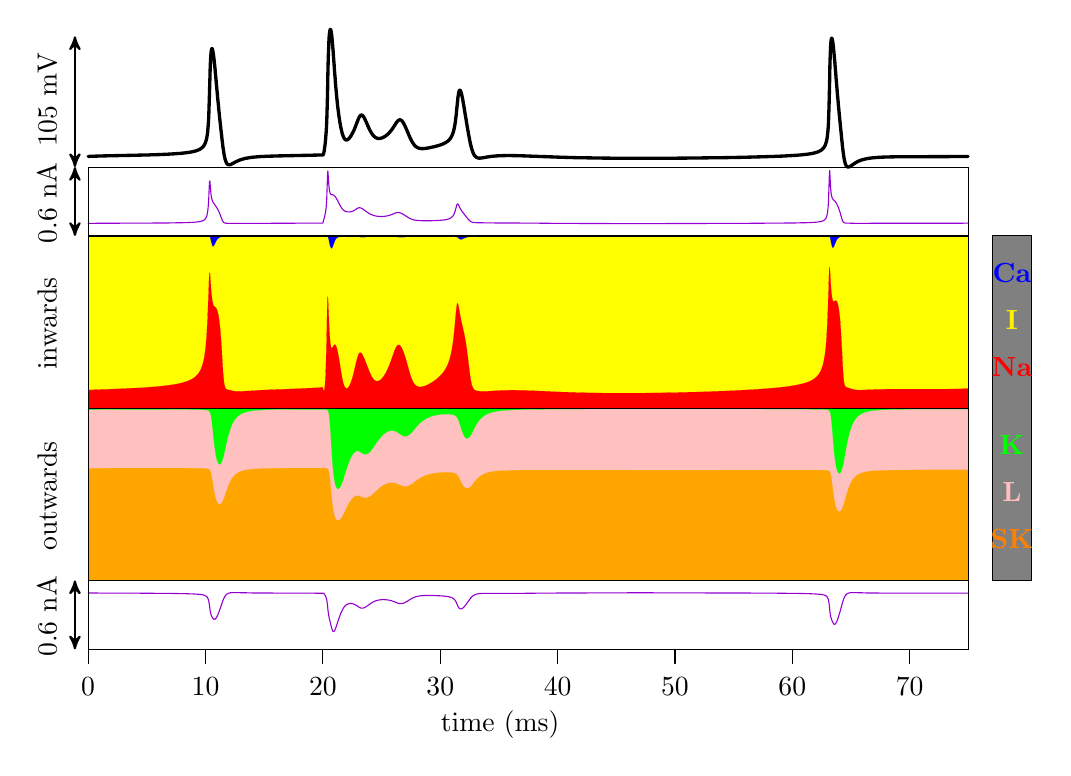
\begin{tikzpicture}[gnuplot]
%% generated with GNUPLOT 5.2p8 (Lua 5.3; terminal rev. Nov 2018, script rev. 108)
%% Fri Feb  5 14:09:46 2021

%%1.750 to 6.125
  %%6.125-1.750 = 4.375
  %%midpoint 3.9375
  %%midpoint of panels 5.03 and 2.84375

\path (0.000,0.000) rectangle (12.500,8.750);
\draw [fill=gray] (12.25,1.75) rectangle (12.75,6.125);

\gpcolor{color=gp lt color border}


\node[gp node center] at (12.5,2.24375) {\color{orange}\textbf{SK}\color{black}};
  \node[gp node center] at (12.5,2.84375) {\color{pink}\textbf{L}\color{black}};
  \node[gp node center] at (12.5,3.44375) {\color{green}\textbf{K}\color{black}};
  
  \node[gp node center] at (12.5,4.43) {\color{red}\textbf{Na}\color{black}};
  \node[gp node center] at (12.5,5.03) {\color{yellow}\textbf{I}\color{black}};
  \node[gp node center] at (12.5,5.63) {\color{blue}\textbf{Ca}\color{black}};
\node[gp node center,rotate=-270] at (0.292,7.874) {105 mV};
\draw [<->,thick] (0.6,7) -- (0.6,8.66);
\gpcolor{rgb color={0.000,0.000,0.000}}
\gpsetlinetype{gp lt border}
\gpsetdashtype{gp dt solid}
\gpsetlinewidth{3.00}
\draw[gp path] (0.768,7.135)--(0.772,7.135)--(0.776,7.135)--(0.779,7.135)--(0.783,7.135)%
  --(0.787,7.136)--(0.790,7.136)--(0.794,7.136)--(0.798,7.136)--(0.802,7.136)--(0.805,7.136)%
  --(0.809,7.137)--(0.813,7.137)--(0.817,7.137)--(0.820,7.137)--(0.824,7.137)--(0.828,7.137)%
  --(0.831,7.138)--(0.835,7.138)--(0.839,7.138)--(0.843,7.138)--(0.846,7.138)--(0.850,7.138)%
  --(0.854,7.138)--(0.858,7.138)--(0.861,7.139)--(0.865,7.139)--(0.869,7.139)--(0.872,7.139)%
  --(0.876,7.139)--(0.880,7.139)--(0.884,7.139)--(0.887,7.139)--(0.891,7.140)--(0.895,7.140)%
  --(0.898,7.140)--(0.902,7.140)--(0.906,7.140)--(0.910,7.140)--(0.913,7.140)--(0.917,7.140)%
  --(0.921,7.140)--(0.925,7.141)--(0.928,7.141)--(0.932,7.141)--(0.936,7.141)--(0.939,7.141)%
  --(0.943,7.141)--(0.947,7.141)--(0.951,7.141)--(0.954,7.141)--(0.958,7.141)--(0.962,7.141)%
  --(0.966,7.142)--(0.969,7.142)--(0.973,7.142)--(0.977,7.142)--(0.980,7.142)--(0.984,7.142)%
  --(0.988,7.142)--(0.992,7.142)--(0.995,7.142)--(0.999,7.142)--(1.003,7.142)--(1.007,7.143)%
  --(1.010,7.143)--(1.014,7.143)--(1.018,7.143)--(1.021,7.143)--(1.025,7.143)--(1.029,7.143)%
  --(1.033,7.143)--(1.036,7.143)--(1.040,7.143)--(1.044,7.143)--(1.048,7.143)--(1.051,7.143)%
  --(1.055,7.144)--(1.059,7.144)--(1.062,7.144)--(1.066,7.144)--(1.070,7.144)--(1.074,7.144)%
  --(1.077,7.144)--(1.081,7.144)--(1.085,7.144)--(1.089,7.144)--(1.092,7.144)--(1.096,7.144)%
  --(1.100,7.144)--(1.103,7.145)--(1.107,7.145)--(1.111,7.145)--(1.115,7.145)--(1.118,7.145)%
  --(1.122,7.145)--(1.126,7.145)--(1.130,7.145)--(1.133,7.145)--(1.137,7.145)--(1.141,7.145)%
  --(1.144,7.145)--(1.148,7.145)--(1.152,7.145)--(1.156,7.146)--(1.159,7.146)--(1.163,7.146)%
  --(1.167,7.146)--(1.171,7.146)--(1.174,7.146)--(1.178,7.146)--(1.182,7.146)--(1.185,7.146)%
  --(1.189,7.146)--(1.193,7.146)--(1.197,7.146)--(1.200,7.146)--(1.204,7.146)--(1.208,7.147)%
  --(1.212,7.147)--(1.215,7.147)--(1.219,7.147)--(1.223,7.147)--(1.226,7.147)--(1.230,7.147)%
  --(1.234,7.147)--(1.238,7.147)--(1.241,7.147)--(1.245,7.147)--(1.249,7.147)--(1.252,7.147)%
  --(1.256,7.147)--(1.260,7.148)--(1.264,7.148)--(1.267,7.148)--(1.271,7.148)--(1.275,7.148)%
  --(1.279,7.148)--(1.282,7.148)--(1.286,7.148)--(1.290,7.148)--(1.293,7.148)--(1.297,7.148)%
  --(1.301,7.148)--(1.305,7.148)--(1.308,7.149)--(1.312,7.149)--(1.316,7.149)--(1.320,7.149)%
  --(1.323,7.149)--(1.327,7.149)--(1.331,7.149)--(1.334,7.149)--(1.338,7.149)--(1.342,7.149)%
  --(1.346,7.149)--(1.349,7.149)--(1.353,7.149)--(1.357,7.150)--(1.361,7.150)--(1.364,7.150)%
  --(1.368,7.150)--(1.372,7.150)--(1.375,7.150)--(1.379,7.150)--(1.383,7.150)--(1.387,7.150)%
  --(1.390,7.150)--(1.394,7.150)--(1.398,7.150)--(1.402,7.151)--(1.405,7.151)--(1.409,7.151)%
  --(1.413,7.151)--(1.416,7.151)--(1.420,7.151)--(1.424,7.151)--(1.428,7.151)--(1.431,7.151)%
  --(1.435,7.151)--(1.439,7.151)--(1.443,7.152)--(1.446,7.152)--(1.450,7.152)--(1.454,7.152)%
  --(1.457,7.152)--(1.461,7.152)--(1.465,7.152)--(1.469,7.152)--(1.472,7.152)--(1.476,7.152)%
  --(1.480,7.152)--(1.484,7.153)--(1.487,7.153)--(1.491,7.153)--(1.495,7.153)--(1.498,7.153)%
  --(1.502,7.153)--(1.506,7.153)--(1.510,7.153)--(1.513,7.153)--(1.517,7.153)--(1.521,7.154)%
  --(1.525,7.154)--(1.528,7.154)--(1.532,7.154)--(1.536,7.154)--(1.539,7.154)--(1.543,7.154)%
  --(1.547,7.154)--(1.551,7.154)--(1.554,7.155)--(1.558,7.155)--(1.562,7.155)--(1.566,7.155)%
  --(1.569,7.155)--(1.573,7.155)--(1.577,7.155)--(1.580,7.155)--(1.584,7.155)--(1.588,7.156)%
  --(1.592,7.156)--(1.595,7.156)--(1.599,7.156)--(1.603,7.156)--(1.606,7.156)--(1.610,7.156)%
  --(1.614,7.156)--(1.618,7.157)--(1.621,7.157)--(1.625,7.157)--(1.629,7.157)--(1.633,7.157)%
  --(1.636,7.157)--(1.640,7.157)--(1.644,7.158)--(1.647,7.158)--(1.651,7.158)--(1.655,7.158)%
  --(1.659,7.158)--(1.662,7.158)--(1.666,7.158)--(1.670,7.158)--(1.674,7.159)--(1.677,7.159)%
  --(1.681,7.159)--(1.685,7.159)--(1.688,7.159)--(1.692,7.159)--(1.696,7.160)--(1.700,7.160)%
  --(1.703,7.160)--(1.707,7.160)--(1.711,7.160)--(1.715,7.160)--(1.718,7.160)--(1.722,7.161)%
  --(1.726,7.161)--(1.729,7.161)--(1.733,7.161)--(1.737,7.161)--(1.741,7.161)--(1.744,7.162)%
  --(1.748,7.162)--(1.752,7.162)--(1.756,7.162)--(1.759,7.162)--(1.763,7.163)--(1.767,7.163)%
  --(1.770,7.163)--(1.774,7.163)--(1.778,7.163)--(1.782,7.163)--(1.785,7.164)--(1.789,7.164)%
  --(1.793,7.164)--(1.797,7.164)--(1.800,7.164)--(1.804,7.165)--(1.808,7.165)--(1.811,7.165)%
  --(1.815,7.165)--(1.819,7.165)--(1.823,7.166)--(1.826,7.166)--(1.830,7.166)--(1.834,7.166)%
  --(1.838,7.167)--(1.841,7.167)--(1.845,7.167)--(1.849,7.167)--(1.852,7.167)--(1.856,7.168)%
  --(1.860,7.168)--(1.864,7.168)--(1.867,7.168)--(1.871,7.169)--(1.875,7.169)--(1.879,7.169)%
  --(1.882,7.169)--(1.886,7.170)--(1.890,7.170)--(1.893,7.170)--(1.897,7.171)--(1.901,7.171)%
  --(1.905,7.171)--(1.908,7.171)--(1.912,7.172)--(1.916,7.172)--(1.920,7.172)--(1.923,7.173)%
  --(1.927,7.173)--(1.931,7.173)--(1.934,7.174)--(1.938,7.174)--(1.942,7.174)--(1.946,7.175)%
  --(1.949,7.175)--(1.953,7.175)--(1.957,7.176)--(1.961,7.176)--(1.964,7.176)--(1.968,7.177)%
  --(1.972,7.177)--(1.975,7.177)--(1.979,7.178)--(1.983,7.178)--(1.987,7.179)--(1.990,7.179)%
  --(1.994,7.179)--(1.998,7.180)--(2.001,7.180)--(2.005,7.181)--(2.009,7.181)--(2.013,7.182)%
  --(2.016,7.182)--(2.020,7.183)--(2.024,7.183)--(2.028,7.184)--(2.031,7.184)--(2.035,7.185)%
  --(2.039,7.185)--(2.042,7.186)--(2.046,7.186)--(2.050,7.187)--(2.054,7.187)--(2.057,7.188)%
  --(2.061,7.189)--(2.065,7.189)--(2.069,7.190)--(2.072,7.191)--(2.076,7.191)--(2.080,7.192)%
  --(2.083,7.193)--(2.087,7.193)--(2.091,7.194)--(2.095,7.195)--(2.098,7.196)--(2.102,7.197)%
  --(2.106,7.197)--(2.110,7.198)--(2.113,7.199)--(2.117,7.200)--(2.121,7.201)--(2.124,7.202)%
  --(2.128,7.203)--(2.132,7.204)--(2.136,7.205)--(2.139,7.206)--(2.143,7.208)--(2.147,7.209)%
  --(2.151,7.210)--(2.154,7.212)--(2.158,7.213)--(2.162,7.214)--(2.165,7.216)--(2.169,7.218)%
  --(2.173,7.219)--(2.177,7.221)--(2.180,7.223)--(2.184,7.225)--(2.188,7.227)--(2.192,7.229)%
  --(2.195,7.232)--(2.199,7.234)--(2.203,7.237)--(2.206,7.239)--(2.210,7.242)--(2.214,7.246)%
  --(2.218,7.249)--(2.221,7.253)--(2.225,7.257)--(2.229,7.261)--(2.233,7.265)--(2.236,7.270)%
  --(2.240,7.276)--(2.244,7.282)--(2.247,7.289)--(2.251,7.296)--(2.255,7.305)--(2.259,7.314)%
  --(2.262,7.325)--(2.266,7.337)--(2.270,7.351)--(2.274,7.368)--(2.277,7.387)--(2.281,7.411)%
  --(2.285,7.440)--(2.288,7.475)--(2.292,7.520)--(2.296,7.578)--(2.300,7.653)--(2.303,7.750)%
  --(2.307,7.872)--(2.311,8.011)--(2.315,8.149)--(2.318,8.265)--(2.322,8.353)--(2.326,8.416)%
  --(2.329,8.458)--(2.333,8.485)--(2.337,8.500)--(2.341,8.505)--(2.344,8.501)--(2.348,8.491)%
  --(2.352,8.475)--(2.355,8.454)--(2.359,8.429)--(2.363,8.400)--(2.367,8.369)--(2.370,8.335)%
  --(2.374,8.298)--(2.378,8.260)--(2.382,8.221)--(2.385,8.181)--(2.389,8.140)--(2.393,8.099)%
  --(2.396,8.058)--(2.400,8.017)--(2.404,7.976)--(2.408,7.935)--(2.411,7.896)--(2.415,7.856)%
  --(2.419,7.818)--(2.423,7.780)--(2.426,7.742)--(2.430,7.705)--(2.434,7.669)--(2.437,7.633)%
  --(2.441,7.598)--(2.445,7.563)--(2.449,7.529)--(2.452,7.494)--(2.456,7.460)--(2.460,7.427)%
  --(2.464,7.394)--(2.467,7.361)--(2.471,7.329)--(2.475,7.299)--(2.478,7.269)--(2.482,7.241)%
  --(2.486,7.214)--(2.490,7.190)--(2.493,7.167)--(2.497,7.146)--(2.501,7.128)--(2.505,7.111)%
  --(2.508,7.097)--(2.512,7.084)--(2.516,7.073)--(2.519,7.064)--(2.523,7.056)--(2.527,7.049)%
  --(2.531,7.044)--(2.534,7.039)--(2.538,7.036)--(2.542,7.033)--(2.546,7.031)--(2.549,7.029)%
  --(2.553,7.029)--(2.557,7.028)--(2.560,7.028)--(2.564,7.029)--(2.568,7.029)--(2.572,7.030)%
  --(2.575,7.031)--(2.579,7.033)--(2.583,7.034)--(2.587,7.036)--(2.590,7.038)--(2.594,7.040)%
  --(2.598,7.042)--(2.601,7.044)--(2.605,7.046)--(2.609,7.048)--(2.613,7.050)--(2.616,7.052)%
  --(2.620,7.054)--(2.624,7.056)--(2.628,7.058)--(2.631,7.060)--(2.635,7.062)--(2.639,7.064)%
  --(2.642,7.066)--(2.646,7.068)--(2.650,7.070)--(2.654,7.072)--(2.657,7.073)--(2.661,7.075)%
  --(2.665,7.077)--(2.669,7.079)--(2.672,7.080)--(2.676,7.082)--(2.680,7.083)--(2.683,7.085)%
  --(2.687,7.086)--(2.691,7.088)--(2.695,7.089)--(2.698,7.091)--(2.702,7.092)--(2.706,7.093)%
  --(2.709,7.094)--(2.713,7.096)--(2.717,7.097)--(2.721,7.098)--(2.724,7.099)--(2.728,7.100)%
  --(2.732,7.101)--(2.736,7.102)--(2.739,7.103)--(2.743,7.104)--(2.747,7.105)--(2.750,7.106)%
  --(2.754,7.107)--(2.758,7.108)--(2.762,7.109)--(2.765,7.110)--(2.769,7.110)--(2.773,7.111)%
  --(2.777,7.112)--(2.780,7.113)--(2.784,7.113)--(2.788,7.114)--(2.791,7.115)--(2.795,7.115)%
  --(2.799,7.116)--(2.803,7.117)--(2.806,7.117)--(2.810,7.118)--(2.814,7.119)--(2.818,7.119)%
  --(2.821,7.120)--(2.825,7.120)--(2.829,7.121)--(2.832,7.121)--(2.836,7.122)--(2.840,7.122)%
  --(2.844,7.123)--(2.847,7.123)--(2.851,7.124)--(2.855,7.124)--(2.859,7.124)--(2.862,7.125)%
  --(2.866,7.125)--(2.870,7.126)--(2.873,7.126)--(2.877,7.126)--(2.881,7.127)--(2.885,7.127)%
  --(2.888,7.127)--(2.892,7.128)--(2.896,7.128)--(2.900,7.128)--(2.903,7.129)--(2.907,7.129)%
  --(2.911,7.129)--(2.914,7.130)--(2.918,7.130)--(2.922,7.130)--(2.926,7.131)--(2.929,7.131)%
  --(2.933,7.131)--(2.937,7.131)--(2.941,7.132)--(2.944,7.132)--(2.948,7.132)--(2.952,7.132)%
  --(2.955,7.133)--(2.959,7.133)--(2.963,7.133)--(2.967,7.133)--(2.970,7.133)--(2.974,7.134)%
  --(2.978,7.134)--(2.982,7.134)--(2.985,7.134)--(2.989,7.134)--(2.993,7.135)--(2.996,7.135)%
  --(3.000,7.135)--(3.004,7.135)--(3.008,7.135)--(3.011,7.136)--(3.015,7.136)--(3.019,7.136)%
  --(3.023,7.136)--(3.026,7.136)--(3.030,7.136)--(3.034,7.137)--(3.037,7.137)--(3.041,7.137)%
  --(3.045,7.137)--(3.049,7.137)--(3.052,7.137)--(3.056,7.137)--(3.060,7.138)--(3.063,7.138)%
  --(3.067,7.138)--(3.071,7.138)--(3.075,7.138)--(3.078,7.138)--(3.082,7.138)--(3.086,7.139)%
  --(3.090,7.139)--(3.093,7.139)--(3.097,7.139)--(3.101,7.139)--(3.104,7.139)--(3.108,7.139)%
  --(3.112,7.139)--(3.116,7.140)--(3.119,7.140)--(3.123,7.140)--(3.127,7.140)--(3.131,7.140)%
  --(3.134,7.140)--(3.138,7.140)--(3.142,7.140)--(3.145,7.140)--(3.149,7.140)--(3.153,7.141)%
  --(3.157,7.141)--(3.160,7.141)--(3.164,7.141)--(3.168,7.141)--(3.172,7.141)--(3.175,7.141)%
  --(3.179,7.141)--(3.183,7.141)--(3.186,7.141)--(3.190,7.142)--(3.194,7.142)--(3.198,7.142)%
  --(3.201,7.142)--(3.205,7.142)--(3.209,7.142)--(3.213,7.142)--(3.216,7.142)--(3.220,7.142)%
  --(3.224,7.142)--(3.227,7.142)--(3.231,7.142)--(3.235,7.143)--(3.239,7.143)--(3.242,7.143)%
  --(3.246,7.143)--(3.250,7.143)--(3.254,7.143)--(3.257,7.143)--(3.261,7.143)--(3.265,7.143)%
  --(3.268,7.143)--(3.272,7.143)--(3.276,7.143)--(3.280,7.144)--(3.283,7.144)--(3.287,7.144)%
  --(3.291,7.144)--(3.295,7.144)--(3.298,7.144)--(3.302,7.144)--(3.306,7.144)--(3.309,7.144)%
  --(3.313,7.144)--(3.317,7.144)--(3.321,7.144)--(3.324,7.144)--(3.328,7.144)--(3.332,7.145)%
  --(3.336,7.145)--(3.339,7.145)--(3.343,7.145)--(3.347,7.145)--(3.350,7.145)--(3.354,7.145)%
  --(3.358,7.145)--(3.362,7.145)--(3.365,7.145)--(3.369,7.145)--(3.373,7.145)--(3.377,7.145)%
  --(3.380,7.146)--(3.384,7.146)--(3.388,7.146)--(3.391,7.146)--(3.395,7.146)--(3.399,7.146)%
  --(3.403,7.146)--(3.406,7.146)--(3.410,7.146)--(3.414,7.146)--(3.417,7.146)--(3.421,7.146)%
  --(3.425,7.146)--(3.429,7.146)--(3.432,7.147)--(3.436,7.147)--(3.440,7.147)--(3.444,7.147)%
  --(3.447,7.147)--(3.451,7.147)--(3.455,7.147)--(3.458,7.147)--(3.462,7.147)--(3.466,7.147)%
  --(3.470,7.147)--(3.473,7.147)--(3.477,7.147)--(3.481,7.147)--(3.485,7.148)--(3.488,7.148)%
  --(3.492,7.148)--(3.496,7.148)--(3.499,7.148)--(3.503,7.148)--(3.507,7.148)--(3.511,7.148)%
  --(3.514,7.148)--(3.518,7.148)--(3.522,7.148)--(3.526,7.148)--(3.529,7.148)--(3.533,7.148)%
  --(3.537,7.149)--(3.540,7.149)--(3.544,7.149)--(3.548,7.149)--(3.552,7.149)--(3.555,7.149)%
  --(3.559,7.149)--(3.563,7.149)--(3.567,7.149)--(3.570,7.149)--(3.574,7.149)--(3.578,7.149)%
  --(3.581,7.150)--(3.585,7.150)--(3.589,7.150)--(3.593,7.150)--(3.596,7.150)--(3.600,7.150)%
  --(3.604,7.150)--(3.608,7.150)--(3.611,7.150)--(3.615,7.150)--(3.619,7.150)--(3.622,7.150)%
  --(3.626,7.151)--(3.630,7.151)--(3.634,7.151)--(3.637,7.151)--(3.641,7.151)--(3.645,7.151)%
  --(3.649,7.151)--(3.652,7.151)--(3.656,7.151)--(3.660,7.151)--(3.663,7.151)--(3.667,7.152)%
  --(3.671,7.152)--(3.675,7.152)--(3.678,7.152)--(3.682,7.152)--(3.686,7.152)--(3.690,7.152)%
  --(3.693,7.152)--(3.697,7.152)--(3.701,7.152)--(3.704,7.152)--(3.708,7.153)--(3.712,7.153)%
  --(3.716,7.153)--(3.719,7.153)--(3.723,7.153)--(3.727,7.153)--(3.731,7.153)--(3.734,7.153)%
  --(3.738,7.153)--(3.742,7.153)--(3.745,7.154)--(3.749,7.154)--(3.753,7.157)--(3.757,7.166)%
  --(3.760,7.179)--(3.764,7.197)--(3.768,7.218)--(3.771,7.243)--(3.775,7.272)--(3.779,7.304)%
  --(3.783,7.341)--(3.786,7.384)--(3.790,7.435)--(3.794,7.496)--(3.798,7.574)--(3.801,7.675)%
  --(3.805,7.809)--(3.809,7.977)--(3.812,8.162)--(3.816,8.330)--(3.820,8.461)--(3.824,8.559)%
  --(3.827,8.631)--(3.831,8.682)--(3.835,8.716)--(3.839,8.738)--(3.842,8.748)--(3.846,8.749)%
  --(3.850,8.741)--(3.853,8.725)--(3.857,8.702)--(3.861,8.673)--(3.865,8.639)--(3.868,8.599)%
  --(3.872,8.556)--(3.876,8.510)--(3.880,8.462)--(3.883,8.412)--(3.887,8.361)--(3.891,8.310)%
  --(3.894,8.259)--(3.898,8.208)--(3.902,8.159)--(3.906,8.111)--(3.909,8.064)--(3.913,8.019)%
  --(3.917,7.976)--(3.921,7.935)--(3.924,7.896)--(3.928,7.858)--(3.932,7.822)--(3.935,7.788)%
  --(3.939,7.755)--(3.943,7.724)--(3.947,7.695)--(3.950,7.667)--(3.954,7.640)--(3.958,7.615)%
  --(3.962,7.591)--(3.965,7.568)--(3.969,7.547)--(3.973,7.526)--(3.976,7.507)--(3.980,7.489)%
  --(3.984,7.472)--(3.988,7.456)--(3.991,7.441)--(3.995,7.428)--(3.999,7.415)--(4.003,7.404)%
  --(4.006,7.393)--(4.010,7.384)--(4.014,7.376)--(4.017,7.369)--(4.021,7.363)--(4.025,7.357)%
  --(4.029,7.353)--(4.032,7.350)--(4.036,7.347)--(4.040,7.345)--(4.044,7.344)--(4.047,7.344)%
  --(4.051,7.344)--(4.055,7.345)--(4.058,7.346)--(4.062,7.348)--(4.066,7.350)--(4.070,7.353)%
  --(4.073,7.356)--(4.077,7.359)--(4.081,7.363)--(4.085,7.367)--(4.088,7.372)--(4.092,7.376)%
  --(4.096,7.381)--(4.099,7.387)--(4.103,7.392)--(4.107,7.398)--(4.111,7.404)--(4.114,7.410)%
  --(4.118,7.417)--(4.122,7.424)--(4.126,7.431)--(4.129,7.438)--(4.133,7.445)--(4.137,7.453)%
  --(4.140,7.461)--(4.144,7.469)--(4.148,7.478)--(4.152,7.486)--(4.155,7.495)--(4.159,7.505)%
  --(4.163,7.514)--(4.166,7.523)--(4.170,7.533)--(4.174,7.543)--(4.178,7.553)--(4.181,7.563)%
  --(4.185,7.573)--(4.189,7.582)--(4.193,7.592)--(4.196,7.601)--(4.200,7.610)--(4.204,7.618)%
  --(4.207,7.626)--(4.211,7.633)--(4.215,7.640)--(4.219,7.645)--(4.222,7.650)--(4.226,7.654)%
  --(4.230,7.657)--(4.234,7.659)--(4.237,7.660)--(4.241,7.660)--(4.245,7.659)--(4.248,7.657)%
  --(4.252,7.655)--(4.256,7.651)--(4.260,7.647)--(4.263,7.642)--(4.267,7.637)--(4.271,7.631)%
  --(4.275,7.624)--(4.278,7.617)--(4.282,7.610)--(4.286,7.602)--(4.289,7.594)--(4.293,7.586)%
  --(4.297,7.578)--(4.301,7.569)--(4.304,7.561)--(4.308,7.552)--(4.312,7.543)--(4.316,7.535)%
  --(4.319,7.526)--(4.323,7.518)--(4.327,7.510)--(4.330,7.501)--(4.334,7.493)--(4.338,7.485)%
  --(4.342,7.478)--(4.345,7.470)--(4.349,7.463)--(4.353,7.456)--(4.357,7.449)--(4.360,7.442)%
  --(4.364,7.436)--(4.368,7.430)--(4.371,7.424)--(4.375,7.419)--(4.379,7.414)--(4.383,7.409)%
  --(4.386,7.404)--(4.390,7.400)--(4.394,7.395)--(4.398,7.392)--(4.401,7.388)--(4.405,7.385)%
  --(4.409,7.382)--(4.412,7.379)--(4.416,7.376)--(4.420,7.374)--(4.424,7.372)--(4.427,7.370)%
  --(4.431,7.369)--(4.435,7.367)--(4.439,7.366)--(4.442,7.365)--(4.446,7.364)--(4.450,7.364)%
  --(4.453,7.363)--(4.457,7.363)--(4.461,7.363)--(4.465,7.363)--(4.468,7.363)--(4.472,7.363)%
  --(4.476,7.364)--(4.480,7.365)--(4.483,7.365)--(4.487,7.366)--(4.491,7.367)--(4.494,7.368)%
  --(4.498,7.370)--(4.502,7.371)--(4.506,7.373)--(4.509,7.374)--(4.513,7.376)--(4.517,7.378)%
  --(4.520,7.379)--(4.524,7.381)--(4.528,7.384)--(4.532,7.386)--(4.535,7.388)--(4.539,7.390)%
  --(4.543,7.393)--(4.547,7.396)--(4.550,7.398)--(4.554,7.401)--(4.558,7.404)--(4.561,7.407)%
  --(4.565,7.410)--(4.569,7.413)--(4.573,7.417)--(4.576,7.420)--(4.580,7.424)--(4.584,7.427)%
  --(4.588,7.431)--(4.591,7.435)--(4.595,7.439)--(4.599,7.443)--(4.602,7.447)--(4.606,7.452)%
  --(4.610,7.456)--(4.614,7.461)--(4.617,7.466)--(4.621,7.471)--(4.625,7.476)--(4.629,7.481)%
  --(4.632,7.486)--(4.636,7.492)--(4.640,7.497)--(4.643,7.503)--(4.647,7.509)--(4.651,7.515)%
  --(4.655,7.520)--(4.658,7.526)--(4.662,7.532)--(4.666,7.538)--(4.670,7.544)--(4.673,7.550)%
  --(4.677,7.555)--(4.681,7.561)--(4.684,7.566)--(4.688,7.571)--(4.692,7.576)--(4.696,7.580)%
  --(4.699,7.584)--(4.703,7.588)--(4.707,7.591)--(4.711,7.594)--(4.714,7.596)--(4.718,7.598)%
  --(4.722,7.599)--(4.725,7.600)--(4.729,7.599)--(4.733,7.599)--(4.737,7.598)--(4.740,7.596)%
  --(4.744,7.593)--(4.748,7.591)--(4.752,7.587)--(4.755,7.583)--(4.759,7.578)--(4.763,7.573)%
  --(4.766,7.568)--(4.770,7.562)--(4.774,7.556)--(4.778,7.549)--(4.781,7.542)--(4.785,7.535)%
  --(4.789,7.527)--(4.793,7.519)--(4.796,7.511)--(4.800,7.503)--(4.804,7.495)--(4.807,7.486)%
  --(4.811,7.478)--(4.815,7.469)--(4.819,7.460)--(4.822,7.451)--(4.826,7.442)--(4.830,7.433)%
  --(4.834,7.425)--(4.837,7.416)--(4.841,7.407)--(4.845,7.398)--(4.848,7.390)--(4.852,7.382)%
  --(4.856,7.373)--(4.860,7.365)--(4.863,7.357)--(4.867,7.350)--(4.871,7.342)--(4.874,7.335)%
  --(4.878,7.328)--(4.882,7.322)--(4.886,7.315)--(4.889,7.309)--(4.893,7.303)--(4.897,7.298)%
  --(4.901,7.293)--(4.904,7.288)--(4.908,7.283)--(4.912,7.278)--(4.915,7.274)--(4.919,7.270)%
  --(4.923,7.267)--(4.927,7.263)--(4.930,7.260)--(4.934,7.257)--(4.938,7.255)--(4.942,7.252)%
  --(4.945,7.250)--(4.949,7.248)--(4.953,7.246)--(4.956,7.244)--(4.960,7.243)--(4.964,7.241)%
  --(4.968,7.240)--(4.971,7.239)--(4.975,7.238)--(4.979,7.237)--(4.983,7.236)--(4.986,7.236)%
  --(4.990,7.235)--(4.994,7.235)--(4.997,7.235)--(5.001,7.234)--(5.005,7.234)--(5.009,7.234)%
  --(5.012,7.234)--(5.016,7.234)--(5.020,7.234)--(5.024,7.234)--(5.027,7.235)--(5.031,7.235)%
  --(5.035,7.235)--(5.038,7.235)--(5.042,7.236)--(5.046,7.236)--(5.050,7.237)--(5.053,7.237)%
  --(5.057,7.238)--(5.061,7.238)--(5.065,7.239)--(5.068,7.239)--(5.072,7.240)--(5.076,7.240)%
  --(5.079,7.241)--(5.083,7.242)--(5.087,7.242)--(5.091,7.243)--(5.094,7.244)--(5.098,7.245)%
  --(5.102,7.245)--(5.106,7.246)--(5.109,7.247)--(5.113,7.248)--(5.117,7.248)--(5.120,7.249)%
  --(5.124,7.250)--(5.128,7.251)--(5.132,7.252)--(5.135,7.252)--(5.139,7.253)--(5.143,7.254)%
  --(5.147,7.255)--(5.150,7.256)--(5.154,7.257)--(5.158,7.257)--(5.161,7.258)--(5.165,7.259)%
  --(5.169,7.260)--(5.173,7.261)--(5.176,7.262)--(5.180,7.263)--(5.184,7.264)--(5.188,7.265)%
  --(5.191,7.266)--(5.195,7.267)--(5.199,7.268)--(5.202,7.269)--(5.206,7.270)--(5.210,7.271)%
  --(5.214,7.272)--(5.217,7.273)--(5.221,7.274)--(5.225,7.276)--(5.228,7.277)--(5.232,7.278)%
  --(5.236,7.279)--(5.240,7.280)--(5.243,7.282)--(5.247,7.283)--(5.251,7.284)--(5.255,7.286)%
  --(5.258,7.287)--(5.262,7.288)--(5.266,7.290)--(5.269,7.291)--(5.273,7.293)--(5.277,7.295)%
  --(5.281,7.296)--(5.284,7.298)--(5.288,7.300)--(5.292,7.302)--(5.296,7.303)--(5.299,7.305)%
  --(5.303,7.307)--(5.307,7.310)--(5.310,7.312)--(5.314,7.314)--(5.318,7.316)--(5.322,7.319)%
  --(5.325,7.322)--(5.329,7.324)--(5.333,7.327)--(5.337,7.330)--(5.340,7.334)--(5.344,7.337)%
  --(5.348,7.340)--(5.351,7.344)--(5.355,7.348)--(5.359,7.353)--(5.363,7.357)--(5.366,7.362)%
  --(5.370,7.367)--(5.374,7.373)--(5.378,7.379)--(5.381,7.386)--(5.385,7.393)--(5.389,7.401)%
  --(5.392,7.409)--(5.396,7.418)--(5.400,7.429)--(5.404,7.440)--(5.407,7.452)--(5.411,7.466)%
  --(5.415,7.482)--(5.419,7.499)--(5.422,7.518)--(5.426,7.539)--(5.430,7.563)--(5.433,7.590)%
  --(5.437,7.620)--(5.441,7.652)--(5.445,7.687)--(5.448,7.725)--(5.452,7.763)--(5.456,7.802)%
  --(5.460,7.838)--(5.463,7.872)--(5.467,7.902)--(5.471,7.927)--(5.474,7.946)--(5.478,7.961)%
  --(5.482,7.971)--(5.486,7.976)--(5.489,7.977)--(5.493,7.974)--(5.497,7.968)--(5.501,7.960)%
  --(5.504,7.949)--(5.508,7.935)--(5.512,7.920)--(5.515,7.904)--(5.519,7.886)--(5.523,7.867)%
  --(5.527,7.847)--(5.530,7.826)--(5.534,7.805)--(5.538,7.783)--(5.542,7.761)--(5.545,7.738)%
  --(5.549,7.716)--(5.553,7.693)--(5.556,7.670)--(5.560,7.647)--(5.564,7.625)--(5.568,7.602)%
  --(5.571,7.580)--(5.575,7.557)--(5.579,7.535)--(5.582,7.513)--(5.586,7.491)--(5.590,7.470)%
  --(5.594,7.449)--(5.597,7.428)--(5.601,7.407)--(5.605,7.387)--(5.609,7.367)--(5.612,7.348)%
  --(5.616,7.330)--(5.620,7.312)--(5.623,7.295)--(5.627,7.279)--(5.631,7.263)--(5.635,7.249)%
  --(5.638,7.235)--(5.642,7.222)--(5.646,7.211)--(5.650,7.200)--(5.653,7.190)--(5.657,7.180)%
  --(5.661,7.172)--(5.664,7.165)--(5.668,7.158)--(5.672,7.151)--(5.676,7.146)--(5.679,7.141)%
  --(5.683,7.137)--(5.687,7.133)--(5.691,7.129)--(5.694,7.126)--(5.698,7.124)--(5.702,7.122)%
  --(5.705,7.120)--(5.709,7.118)--(5.713,7.117)--(5.717,7.116)--(5.720,7.115)--(5.724,7.114)%
  --(5.728,7.114)--(5.732,7.113)--(5.735,7.113)--(5.739,7.113)--(5.743,7.113)--(5.746,7.113)%
  --(5.750,7.114)--(5.754,7.114)--(5.758,7.114)--(5.761,7.115)--(5.765,7.115)--(5.769,7.116)%
  --(5.773,7.116)--(5.776,7.117)--(5.780,7.117)--(5.784,7.118)--(5.787,7.119)--(5.791,7.119)%
  --(5.795,7.120)--(5.799,7.121)--(5.802,7.121)--(5.806,7.122)--(5.810,7.123)--(5.814,7.123)%
  --(5.817,7.124)--(5.821,7.125)--(5.825,7.125)--(5.828,7.126)--(5.832,7.127)--(5.836,7.127)%
  --(5.840,7.128)--(5.843,7.129)--(5.847,7.129)--(5.851,7.130)--(5.855,7.130)--(5.858,7.131)%
  --(5.862,7.131)--(5.866,7.132)--(5.869,7.133)--(5.873,7.133)--(5.877,7.134)--(5.881,7.134)%
  --(5.884,7.135)--(5.888,7.135)--(5.892,7.135)--(5.896,7.136)--(5.899,7.136)--(5.903,7.137)%
  --(5.907,7.137)--(5.910,7.138)--(5.914,7.138)--(5.918,7.138)--(5.922,7.139)--(5.925,7.139)%
  --(5.929,7.139)--(5.933,7.140)--(5.936,7.140)--(5.940,7.140)--(5.944,7.141)--(5.948,7.141)%
  --(5.951,7.141)--(5.955,7.141)--(5.959,7.142)--(5.963,7.142)--(5.966,7.142)--(5.970,7.142)%
  --(5.974,7.143)--(5.977,7.143)--(5.981,7.143)--(5.985,7.143)--(5.989,7.143)--(5.992,7.143)%
  --(5.996,7.144)--(6.000,7.144)--(6.004,7.144)--(6.007,7.144)--(6.011,7.144)--(6.015,7.144)%
  --(6.018,7.144)--(6.022,7.145)--(6.026,7.145)--(6.030,7.145)--(6.033,7.145)--(6.037,7.145)%
  --(6.041,7.145)--(6.045,7.145)--(6.048,7.145)--(6.052,7.145)--(6.056,7.145)--(6.059,7.145)%
  --(6.063,7.145)--(6.067,7.146)--(6.071,7.146)--(6.074,7.146)--(6.078,7.146)--(6.082,7.146)%
  --(6.086,7.146)--(6.089,7.146)--(6.093,7.146)--(6.097,7.146)--(6.100,7.146)--(6.104,7.146)%
  --(6.108,7.146)--(6.112,7.146)--(6.115,7.146)--(6.119,7.146)--(6.123,7.146)--(6.127,7.146)%
  --(6.130,7.146)--(6.134,7.146)--(6.138,7.146)--(6.141,7.146)--(6.145,7.146)--(6.149,7.146)%
  --(6.153,7.145)--(6.156,7.145)--(6.160,7.145)--(6.164,7.145)--(6.168,7.145)--(6.171,7.145)%
  --(6.175,7.145)--(6.179,7.145)--(6.182,7.145)--(6.186,7.145)--(6.190,7.145)--(6.194,7.145)%
  --(6.197,7.145)--(6.201,7.145)--(6.205,7.145)--(6.209,7.144)--(6.212,7.144)--(6.216,7.144)%
  --(6.220,7.144)--(6.223,7.144)--(6.227,7.144)--(6.231,7.144)--(6.235,7.144)--(6.238,7.144)%
  --(6.242,7.144)--(6.246,7.144)--(6.250,7.143)--(6.253,7.143)--(6.257,7.143)--(6.261,7.143)%
  --(6.264,7.143)--(6.268,7.143)--(6.272,7.143)--(6.276,7.143)--(6.279,7.143)--(6.283,7.142)%
  --(6.287,7.142)--(6.291,7.142)--(6.294,7.142)--(6.298,7.142)--(6.302,7.142)--(6.305,7.142)%
  --(6.309,7.142)--(6.313,7.142)--(6.317,7.141)--(6.320,7.141)--(6.324,7.141)--(6.328,7.141)%
  --(6.331,7.141)--(6.335,7.141)--(6.339,7.141)--(6.343,7.141)--(6.346,7.140)--(6.350,7.140)%
  --(6.354,7.140)--(6.358,7.140)--(6.361,7.140)--(6.365,7.140)--(6.369,7.140)--(6.372,7.139)%
  --(6.376,7.139)--(6.380,7.139)--(6.384,7.139)--(6.387,7.139)--(6.391,7.139)--(6.395,7.139)%
  --(6.399,7.138)--(6.402,7.138)--(6.406,7.138)--(6.410,7.138)--(6.413,7.138)--(6.417,7.138)%
  --(6.421,7.138)--(6.425,7.138)--(6.428,7.137)--(6.432,7.137)--(6.436,7.137)--(6.440,7.137)%
  --(6.443,7.137)--(6.447,7.137)--(6.451,7.137)--(6.454,7.136)--(6.458,7.136)--(6.462,7.136)%
  --(6.466,7.136)--(6.469,7.136)--(6.473,7.136)--(6.477,7.136)--(6.481,7.135)--(6.484,7.135)%
  --(6.488,7.135)--(6.492,7.135)--(6.495,7.135)--(6.499,7.135)--(6.503,7.134)--(6.507,7.134)%
  --(6.510,7.134)--(6.514,7.134)--(6.518,7.134)--(6.522,7.134)--(6.525,7.134)--(6.529,7.133)%
  --(6.533,7.133)--(6.536,7.133)--(6.540,7.133)--(6.544,7.133)--(6.548,7.133)--(6.551,7.133)%
  --(6.555,7.132)--(6.559,7.132)--(6.563,7.132)--(6.566,7.132)--(6.570,7.132)--(6.574,7.132)%
  --(6.577,7.132)--(6.581,7.132)--(6.585,7.131)--(6.589,7.131)--(6.592,7.131)--(6.596,7.131)%
  --(6.600,7.131)--(6.604,7.131)--(6.607,7.131)--(6.611,7.130)--(6.615,7.130)--(6.618,7.130)%
  --(6.622,7.130)--(6.626,7.130)--(6.630,7.130)--(6.633,7.130)--(6.637,7.129)--(6.641,7.129)%
  --(6.645,7.129)--(6.648,7.129)--(6.652,7.129)--(6.656,7.129)--(6.659,7.129)--(6.663,7.129)%
  --(6.667,7.128)--(6.671,7.128)--(6.674,7.128)--(6.678,7.128)--(6.682,7.128)--(6.685,7.128)%
  --(6.689,7.128)--(6.693,7.127)--(6.697,7.127)--(6.700,7.127)--(6.704,7.127)--(6.708,7.127)%
  --(6.712,7.127)--(6.715,7.127)--(6.719,7.127)--(6.723,7.126)--(6.726,7.126)--(6.730,7.126)%
  --(6.734,7.126)--(6.738,7.126)--(6.741,7.126)--(6.745,7.126)--(6.749,7.126)--(6.753,7.125)%
  --(6.756,7.125)--(6.760,7.125)--(6.764,7.125)--(6.767,7.125)--(6.771,7.125)--(6.775,7.125)%
  --(6.779,7.125)--(6.782,7.125)--(6.786,7.124)--(6.790,7.124)--(6.794,7.124)--(6.797,7.124)%
  --(6.801,7.124)--(6.805,7.124)--(6.808,7.124)--(6.812,7.124)--(6.816,7.124)--(6.820,7.123)%
  --(6.823,7.123)--(6.827,7.123)--(6.831,7.123)--(6.835,7.123)--(6.838,7.123)--(6.842,7.123)%
  --(6.846,7.123)--(6.849,7.123)--(6.853,7.122)--(6.857,7.122)--(6.861,7.122)--(6.864,7.122)%
  --(6.868,7.122)--(6.872,7.122)--(6.876,7.122)--(6.879,7.122)--(6.883,7.122)--(6.887,7.121)%
  --(6.890,7.121)--(6.894,7.121)--(6.898,7.121)--(6.902,7.121)--(6.905,7.121)--(6.909,7.121)%
  --(6.913,7.121)--(6.917,7.121)--(6.920,7.121)--(6.924,7.121)--(6.928,7.120)--(6.931,7.120)%
  --(6.935,7.120)--(6.939,7.120)--(6.943,7.120)--(6.946,7.120)--(6.950,7.120)--(6.954,7.120)%
  --(6.958,7.120)--(6.961,7.120)--(6.965,7.120)--(6.969,7.119)--(6.972,7.119)--(6.976,7.119)%
  --(6.980,7.119)--(6.984,7.119)--(6.987,7.119)--(6.991,7.119)--(6.995,7.119)--(6.999,7.119)%
  --(7.002,7.119)--(7.006,7.119)--(7.010,7.118)--(7.013,7.118)--(7.017,7.118)--(7.021,7.118)%
  --(7.025,7.118)--(7.028,7.118)--(7.032,7.118)--(7.036,7.118)--(7.039,7.118)--(7.043,7.118)%
  --(7.047,7.118)--(7.051,7.118)--(7.054,7.118)--(7.058,7.117)--(7.062,7.117)--(7.066,7.117)%
  --(7.069,7.117)--(7.073,7.117)--(7.077,7.117)--(7.080,7.117)--(7.084,7.117)--(7.088,7.117)%
  --(7.092,7.117)--(7.095,7.117)--(7.099,7.117)--(7.103,7.117)--(7.107,7.116)--(7.110,7.116)%
  --(7.114,7.116)--(7.118,7.116)--(7.121,7.116)--(7.125,7.116)--(7.129,7.116)--(7.133,7.116)%
  --(7.136,7.116)--(7.140,7.116)--(7.144,7.116)--(7.148,7.116)--(7.151,7.116)--(7.155,7.116)%
  --(7.159,7.116)--(7.162,7.116)--(7.166,7.115)--(7.170,7.115)--(7.174,7.115)--(7.177,7.115)%
  --(7.181,7.115)--(7.185,7.115)--(7.189,7.115)--(7.192,7.115)--(7.196,7.115)--(7.200,7.115)%
  --(7.203,7.115)--(7.207,7.115)--(7.211,7.115)--(7.215,7.115)--(7.218,7.115)--(7.222,7.115)%
  --(7.226,7.115)--(7.230,7.114)--(7.233,7.114)--(7.237,7.114)--(7.241,7.114)--(7.244,7.114)%
  --(7.248,7.114)--(7.252,7.114)--(7.256,7.114)--(7.259,7.114)--(7.263,7.114)--(7.267,7.114)%
  --(7.271,7.114)--(7.274,7.114)--(7.278,7.114)--(7.282,7.114)--(7.285,7.114)--(7.289,7.114)%
  --(7.293,7.114)--(7.297,7.114)--(7.300,7.114)--(7.304,7.113)--(7.308,7.113)--(7.312,7.113)%
  --(7.315,7.113)--(7.319,7.113)--(7.323,7.113)--(7.326,7.113)--(7.330,7.113)--(7.334,7.113)%
  --(7.338,7.113)--(7.341,7.113)--(7.345,7.113)--(7.349,7.113)--(7.353,7.113)--(7.356,7.113)%
  --(7.360,7.113)--(7.364,7.113)--(7.367,7.113)--(7.371,7.113)--(7.375,7.113)--(7.379,7.113)%
  --(7.382,7.113)--(7.386,7.113)--(7.390,7.113)--(7.393,7.113)--(7.397,7.112)--(7.401,7.112)%
  --(7.405,7.112)--(7.408,7.112)--(7.412,7.112)--(7.416,7.112)--(7.420,7.112)--(7.423,7.112)%
  --(7.427,7.112)--(7.431,7.112)--(7.434,7.112)--(7.438,7.112)--(7.442,7.112)--(7.446,7.112)%
  --(7.449,7.112)--(7.453,7.112)--(7.457,7.112)--(7.461,7.112)--(7.464,7.112)--(7.468,7.112)%
  --(7.472,7.112)--(7.475,7.112)--(7.479,7.112)--(7.483,7.112)--(7.487,7.112)--(7.490,7.112)%
  --(7.494,7.112)--(7.498,7.112)--(7.502,7.112)--(7.505,7.112)--(7.509,7.112)--(7.513,7.112)%
  --(7.516,7.112)--(7.520,7.112)--(7.524,7.112)--(7.528,7.112)--(7.531,7.111)--(7.535,7.111)%
  --(7.539,7.111)--(7.543,7.111)--(7.546,7.111)--(7.550,7.111)--(7.554,7.111)--(7.557,7.111)%
  --(7.561,7.111)--(7.565,7.111)--(7.569,7.111)--(7.572,7.111)--(7.576,7.111)--(7.580,7.111)%
  --(7.584,7.111)--(7.587,7.111)--(7.591,7.111)--(7.595,7.111)--(7.598,7.111)--(7.602,7.111)%
  --(7.606,7.111)--(7.610,7.111)--(7.613,7.111)--(7.617,7.111)--(7.621,7.111)--(7.625,7.111)%
  --(7.628,7.111)--(7.632,7.111)--(7.636,7.111)--(7.639,7.111)--(7.643,7.111)--(7.647,7.111)%
  --(7.651,7.111)--(7.654,7.111)--(7.658,7.111)--(7.662,7.111)--(7.666,7.111)--(7.669,7.111)%
  --(7.673,7.111)--(7.677,7.111)--(7.680,7.111)--(7.684,7.111)--(7.688,7.111)--(7.692,7.111)%
  --(7.695,7.111)--(7.699,7.111)--(7.703,7.111)--(7.707,7.111)--(7.710,7.111)--(7.714,7.111)%
  --(7.718,7.111)--(7.721,7.111)--(7.725,7.111)--(7.729,7.111)--(7.733,7.111)--(7.736,7.111)%
  --(7.740,7.111)--(7.744,7.111)--(7.747,7.111)--(7.751,7.111)--(7.755,7.111)--(7.759,7.111)%
  --(7.762,7.111)--(7.766,7.111)--(7.770,7.111)--(7.774,7.111)--(7.777,7.111)--(7.781,7.111)%
  --(7.785,7.111)--(7.788,7.111)--(7.792,7.111)--(7.796,7.111)--(7.800,7.111)--(7.803,7.111)%
  --(7.807,7.111)--(7.811,7.111)--(7.815,7.111)--(7.818,7.111)--(7.822,7.111)--(7.826,7.111)%
  --(7.829,7.111)--(7.833,7.111)--(7.837,7.111)--(7.841,7.111)--(7.844,7.111)--(7.848,7.111)%
  --(7.852,7.111)--(7.856,7.111)--(7.859,7.111)--(7.863,7.111)--(7.867,7.111)--(7.870,7.111)%
  --(7.874,7.111)--(7.878,7.111)--(7.882,7.111)--(7.885,7.111)--(7.889,7.111)--(7.893,7.111)%
  --(7.897,7.111)--(7.900,7.111)--(7.904,7.111)--(7.908,7.111)--(7.911,7.111)--(7.915,7.111)%
  --(7.919,7.111)--(7.923,7.111)--(7.926,7.111)--(7.930,7.111)--(7.934,7.111)--(7.938,7.111)%
  --(7.941,7.111)--(7.945,7.111)--(7.949,7.111)--(7.952,7.111)--(7.956,7.111)--(7.960,7.111)%
  --(7.964,7.111)--(7.967,7.111)--(7.971,7.111)--(7.975,7.111)--(7.979,7.111)--(7.982,7.111)%
  --(7.986,7.111)--(7.990,7.111)--(7.993,7.111)--(7.997,7.111)--(8.001,7.111)--(8.005,7.111)%
  --(8.008,7.111)--(8.012,7.111)--(8.016,7.111)--(8.020,7.111)--(8.023,7.111)--(8.027,7.111)%
  --(8.031,7.111)--(8.034,7.111)--(8.038,7.111)--(8.042,7.111)--(8.046,7.111)--(8.049,7.111)%
  --(8.053,7.111)--(8.057,7.111)--(8.061,7.111)--(8.064,7.111)--(8.068,7.111)--(8.072,7.111)%
  --(8.075,7.111)--(8.079,7.111)--(8.083,7.111)--(8.087,7.111)--(8.090,7.111)--(8.094,7.111)%
  --(8.098,7.112)--(8.101,7.112)--(8.105,7.112)--(8.109,7.112)--(8.113,7.112)--(8.116,7.112)%
  --(8.120,7.112)--(8.124,7.112)--(8.128,7.112)--(8.131,7.112)--(8.135,7.112)--(8.139,7.112)%
  --(8.142,7.112)--(8.146,7.112)--(8.150,7.112)--(8.154,7.112)--(8.157,7.112)--(8.161,7.112)%
  --(8.165,7.112)--(8.169,7.112)--(8.172,7.112)--(8.176,7.112)--(8.180,7.112)--(8.183,7.112)%
  --(8.187,7.112)--(8.191,7.112)--(8.195,7.112)--(8.198,7.112)--(8.202,7.112)--(8.206,7.112)%
  --(8.210,7.112)--(8.213,7.112)--(8.217,7.112)--(8.221,7.112)--(8.224,7.112)--(8.228,7.112)%
  --(8.232,7.112)--(8.236,7.112)--(8.239,7.112)--(8.243,7.112)--(8.247,7.112)--(8.251,7.112)%
  --(8.254,7.113)--(8.258,7.113)--(8.262,7.113)--(8.265,7.113)--(8.269,7.113)--(8.273,7.113)%
  --(8.277,7.113)--(8.280,7.113)--(8.284,7.113)--(8.288,7.113)--(8.292,7.113)--(8.295,7.113)%
  --(8.299,7.113)--(8.303,7.113)--(8.306,7.113)--(8.310,7.113)--(8.314,7.113)--(8.318,7.113)%
  --(8.321,7.113)--(8.325,7.113)--(8.329,7.113)--(8.333,7.113)--(8.336,7.113)--(8.340,7.113)%
  --(8.344,7.113)--(8.347,7.113)--(8.351,7.113)--(8.355,7.113)--(8.359,7.113)--(8.362,7.113)%
  --(8.366,7.113)--(8.370,7.113)--(8.374,7.114)--(8.377,7.114)--(8.381,7.114)--(8.385,7.114)%
  --(8.388,7.114)--(8.392,7.114)--(8.396,7.114)--(8.400,7.114)--(8.403,7.114)--(8.407,7.114)%
  --(8.411,7.114)--(8.415,7.114)--(8.418,7.114)--(8.422,7.114)--(8.426,7.114)--(8.429,7.114)%
  --(8.433,7.114)--(8.437,7.114)--(8.441,7.114)--(8.444,7.114)--(8.448,7.114)--(8.452,7.114)%
  --(8.456,7.114)--(8.459,7.114)--(8.463,7.114)--(8.467,7.114)--(8.470,7.114)--(8.474,7.115)%
  --(8.478,7.115)--(8.482,7.115)--(8.485,7.115)--(8.489,7.115)--(8.493,7.115)--(8.496,7.115)%
  --(8.500,7.115)--(8.504,7.115)--(8.508,7.115)--(8.511,7.115)--(8.515,7.115)--(8.519,7.115)%
  --(8.523,7.115)--(8.526,7.115)--(8.530,7.115)--(8.534,7.115)--(8.537,7.115)--(8.541,7.115)%
  --(8.545,7.115)--(8.549,7.115)--(8.552,7.115)--(8.556,7.115)--(8.560,7.115)--(8.564,7.116)%
  --(8.567,7.116)--(8.571,7.116)--(8.575,7.116)--(8.578,7.116)--(8.582,7.116)--(8.586,7.116)%
  --(8.590,7.116)--(8.593,7.116)--(8.597,7.116)--(8.601,7.116)--(8.605,7.116)--(8.608,7.116)%
  --(8.612,7.116)--(8.616,7.116)--(8.619,7.116)--(8.623,7.116)--(8.627,7.116)--(8.631,7.116)%
  --(8.634,7.116)--(8.638,7.116)--(8.642,7.117)--(8.646,7.117)--(8.649,7.117)--(8.653,7.117)%
  --(8.657,7.117)--(8.660,7.117)--(8.664,7.117)--(8.668,7.117)--(8.672,7.117)--(8.675,7.117)%
  --(8.679,7.117)--(8.683,7.117)--(8.687,7.117)--(8.690,7.117)--(8.694,7.117)--(8.698,7.117)%
  --(8.701,7.117)--(8.705,7.117)--(8.709,7.117)--(8.713,7.117)--(8.716,7.118)--(8.720,7.118)%
  --(8.724,7.118)--(8.728,7.118)--(8.731,7.118)--(8.735,7.118)--(8.739,7.118)--(8.742,7.118)%
  --(8.746,7.118)--(8.750,7.118)--(8.754,7.118)--(8.757,7.118)--(8.761,7.118)--(8.765,7.118)%
  --(8.769,7.118)--(8.772,7.118)--(8.776,7.118)--(8.780,7.119)--(8.783,7.119)--(8.787,7.119)%
  --(8.791,7.119)--(8.795,7.119)--(8.798,7.119)--(8.802,7.119)--(8.806,7.119)--(8.810,7.119)%
  --(8.813,7.119)--(8.817,7.119)--(8.821,7.119)--(8.824,7.119)--(8.828,7.119)--(8.832,7.119)%
  --(8.836,7.119)--(8.839,7.119)--(8.843,7.120)--(8.847,7.120)--(8.850,7.120)--(8.854,7.120)%
  --(8.858,7.120)--(8.862,7.120)--(8.865,7.120)--(8.869,7.120)--(8.873,7.120)--(8.877,7.120)%
  --(8.880,7.120)--(8.884,7.120)--(8.888,7.120)--(8.891,7.120)--(8.895,7.120)--(8.899,7.120)%
  --(8.903,7.121)--(8.906,7.121)--(8.910,7.121)--(8.914,7.121)--(8.918,7.121)--(8.921,7.121)%
  --(8.925,7.121)--(8.929,7.121)--(8.932,7.121)--(8.936,7.121)--(8.940,7.121)--(8.944,7.121)%
  --(8.947,7.121)--(8.951,7.121)--(8.955,7.121)--(8.959,7.122)--(8.962,7.122)--(8.966,7.122)%
  --(8.970,7.122)--(8.973,7.122)--(8.977,7.122)--(8.981,7.122)--(8.985,7.122)--(8.988,7.122)%
  --(8.992,7.122)--(8.996,7.122)--(9.000,7.122)--(9.003,7.122)--(9.007,7.122)--(9.011,7.123)%
  --(9.014,7.123)--(9.018,7.123)--(9.022,7.123)--(9.026,7.123)--(9.029,7.123)--(9.033,7.123)%
  --(9.037,7.123)--(9.041,7.123)--(9.044,7.123)--(9.048,7.123)--(9.052,7.123)--(9.055,7.123)%
  --(9.059,7.124)--(9.063,7.124)--(9.067,7.124)--(9.070,7.124)--(9.074,7.124)--(9.078,7.124)%
  --(9.082,7.124)--(9.085,7.124)--(9.089,7.124)--(9.093,7.124)--(9.096,7.124)--(9.100,7.124)%
  --(9.104,7.125)--(9.108,7.125)--(9.111,7.125)--(9.115,7.125)--(9.119,7.125)--(9.123,7.125)%
  --(9.126,7.125)--(9.130,7.125)--(9.134,7.125)--(9.137,7.125)--(9.141,7.125)--(9.145,7.125)%
  --(9.149,7.126)--(9.152,7.126)--(9.156,7.126)--(9.160,7.126)--(9.164,7.126)--(9.167,7.126)%
  --(9.171,7.126)--(9.175,7.126)--(9.178,7.126)--(9.182,7.126)--(9.186,7.126)--(9.190,7.127)%
  --(9.193,7.127)--(9.197,7.127)--(9.201,7.127)--(9.204,7.127)--(9.208,7.127)--(9.212,7.127)%
  --(9.216,7.127)--(9.219,7.127)--(9.223,7.127)--(9.227,7.127)--(9.231,7.128)--(9.234,7.128)%
  --(9.238,7.128)--(9.242,7.128)--(9.245,7.128)--(9.249,7.128)--(9.253,7.128)--(9.257,7.128)%
  --(9.260,7.128)--(9.264,7.128)--(9.268,7.129)--(9.272,7.129)--(9.275,7.129)--(9.279,7.129)%
  --(9.283,7.129)--(9.286,7.129)--(9.290,7.129)--(9.294,7.129)--(9.298,7.129)--(9.301,7.129)%
  --(9.305,7.130)--(9.309,7.130)--(9.313,7.130)--(9.316,7.130)--(9.320,7.130)--(9.324,7.130)%
  --(9.327,7.130)--(9.331,7.130)--(9.335,7.130)--(9.339,7.131)--(9.342,7.131)--(9.346,7.131)%
  --(9.350,7.131)--(9.354,7.131)--(9.357,7.131)--(9.361,7.131)--(9.365,7.131)--(9.368,7.131)%
  --(9.372,7.132)--(9.376,7.132)--(9.380,7.132)--(9.383,7.132)--(9.387,7.132)--(9.391,7.132)%
  --(9.395,7.132)--(9.398,7.132)--(9.402,7.132)--(9.406,7.133)--(9.409,7.133)--(9.413,7.133)%
  --(9.417,7.133)--(9.421,7.133)--(9.424,7.133)--(9.428,7.133)--(9.432,7.133)--(9.436,7.134)%
  --(9.439,7.134)--(9.443,7.134)--(9.447,7.134)--(9.450,7.134)--(9.454,7.134)--(9.458,7.134)%
  --(9.462,7.135)--(9.465,7.135)--(9.469,7.135)--(9.473,7.135)--(9.477,7.135)--(9.480,7.135)%
  --(9.484,7.135)--(9.488,7.135)--(9.491,7.136)--(9.495,7.136)--(9.499,7.136)--(9.503,7.136)%
  --(9.506,7.136)--(9.510,7.136)--(9.514,7.136)--(9.518,7.137)--(9.521,7.137)--(9.525,7.137)%
  --(9.529,7.137)--(9.532,7.137)--(9.536,7.137)--(9.540,7.138)--(9.544,7.138)--(9.547,7.138)%
  --(9.551,7.138)--(9.555,7.138)--(9.558,7.138)--(9.562,7.138)--(9.566,7.139)--(9.570,7.139)%
  --(9.573,7.139)--(9.577,7.139)--(9.581,7.139)--(9.585,7.139)--(9.588,7.140)--(9.592,7.140)%
  --(9.596,7.140)--(9.599,7.140)--(9.603,7.140)--(9.607,7.141)--(9.611,7.141)--(9.614,7.141)%
  --(9.618,7.141)--(9.622,7.141)--(9.626,7.141)--(9.629,7.142)--(9.633,7.142)--(9.637,7.142)%
  --(9.640,7.142)--(9.644,7.142)--(9.648,7.143)--(9.652,7.143)--(9.655,7.143)--(9.659,7.143)%
  --(9.663,7.143)--(9.667,7.144)--(9.670,7.144)--(9.674,7.144)--(9.678,7.144)--(9.681,7.144)%
  --(9.685,7.145)--(9.689,7.145)--(9.693,7.145)--(9.696,7.145)--(9.700,7.145)--(9.704,7.146)%
  --(9.708,7.146)--(9.711,7.146)--(9.715,7.146)--(9.719,7.147)--(9.722,7.147)--(9.726,7.147)%
  --(9.730,7.147)--(9.734,7.148)--(9.737,7.148)--(9.741,7.148)--(9.745,7.148)--(9.749,7.149)%
  --(9.752,7.149)--(9.756,7.149)--(9.760,7.149)--(9.763,7.150)--(9.767,7.150)--(9.771,7.150)%
  --(9.775,7.150)--(9.778,7.151)--(9.782,7.151)--(9.786,7.151)--(9.790,7.152)--(9.793,7.152)%
  --(9.797,7.152)--(9.801,7.153)--(9.804,7.153)--(9.808,7.153)--(9.812,7.153)--(9.816,7.154)%
  --(9.819,7.154)--(9.823,7.154)--(9.827,7.155)--(9.831,7.155)--(9.834,7.156)--(9.838,7.156)%
  --(9.842,7.156)--(9.845,7.157)--(9.849,7.157)--(9.853,7.157)--(9.857,7.158)--(9.860,7.158)%
  --(9.864,7.159)--(9.868,7.159)--(9.872,7.159)--(9.875,7.160)--(9.879,7.160)--(9.883,7.161)%
  --(9.886,7.161)--(9.890,7.162)--(9.894,7.162)--(9.898,7.163)--(9.901,7.163)--(9.905,7.163)%
  --(9.909,7.164)--(9.912,7.165)--(9.916,7.165)--(9.920,7.166)--(9.924,7.166)--(9.927,7.167)%
  --(9.931,7.167)--(9.935,7.168)--(9.939,7.168)--(9.942,7.169)--(9.946,7.170)--(9.950,7.170)%
  --(9.953,7.171)--(9.957,7.172)--(9.961,7.172)--(9.965,7.173)--(9.968,7.174)--(9.972,7.175)%
  --(9.976,7.175)--(9.980,7.176)--(9.983,7.177)--(9.987,7.178)--(9.991,7.179)--(9.994,7.180)%
  --(9.998,7.181)--(10.002,7.182)--(10.006,7.183)--(10.009,7.184)--(10.013,7.185)--(10.017,7.186)%
  --(10.021,7.187)--(10.024,7.189)--(10.028,7.190)--(10.032,7.191)--(10.035,7.193)--(10.039,7.194)%
  --(10.043,7.196)--(10.047,7.197)--(10.050,7.199)--(10.054,7.201)--(10.058,7.203)--(10.062,7.205)%
  --(10.065,7.207)--(10.069,7.209)--(10.073,7.211)--(10.076,7.214)--(10.080,7.216)--(10.084,7.219)%
  --(10.088,7.222)--(10.091,7.225)--(10.095,7.229)--(10.099,7.233)--(10.103,7.237)--(10.106,7.241)%
  --(10.110,7.246)--(10.114,7.251)--(10.117,7.257)--(10.121,7.263)--(10.125,7.270)--(10.129,7.279)%
  --(10.132,7.288)--(10.136,7.298)--(10.140,7.310)--(10.144,7.324)--(10.147,7.340)--(10.151,7.359)%
  --(10.155,7.383)--(10.158,7.412)--(10.162,7.449)--(10.166,7.497)--(10.170,7.561)--(10.173,7.647)%
  --(10.177,7.766)--(10.181,7.924)--(10.185,8.108)--(10.188,8.281)--(10.192,8.414)--(10.196,8.507)%
  --(10.199,8.568)--(10.203,8.606)--(10.207,8.628)--(10.211,8.636)--(10.214,8.634)--(10.218,8.623)%
  --(10.222,8.606)--(10.226,8.583)--(10.229,8.554)--(10.233,8.522)--(10.237,8.486)--(10.240,8.448)%
  --(10.244,8.406)--(10.248,8.363)--(10.252,8.319)--(10.255,8.274)--(10.259,8.228)--(10.263,8.181)%
  --(10.266,8.135)--(10.270,8.089)--(10.274,8.044)--(10.278,7.999)--(10.281,7.955)--(10.285,7.911)%
  --(10.289,7.869)--(10.293,7.827)--(10.296,7.786)--(10.300,7.746)--(10.304,7.707)--(10.307,7.668)%
  --(10.311,7.629)--(10.315,7.591)--(10.319,7.553)--(10.322,7.515)--(10.326,7.478)--(10.330,7.440)%
  --(10.334,7.403)--(10.337,7.366)--(10.341,7.330)--(10.345,7.294)--(10.348,7.260)--(10.352,7.227)%
  --(10.356,7.196)--(10.360,7.168)--(10.363,7.142)--(10.367,7.118)--(10.371,7.098)--(10.375,7.079)%
  --(10.378,7.064)--(10.382,7.050)--(10.386,7.039)--(10.389,7.029)--(10.393,7.021)--(10.397,7.015)%
  --(10.401,7.010)--(10.404,7.006)--(10.408,7.004)--(10.412,7.002)--(10.416,7.000)--(10.419,7.000)%
  --(10.423,7.000)--(10.427,7.001)--(10.430,7.002)--(10.434,7.003)--(10.438,7.005)--(10.442,7.006)%
  --(10.445,7.008)--(10.449,7.011)--(10.453,7.013)--(10.457,7.015)--(10.460,7.018)--(10.464,7.021)%
  --(10.468,7.023)--(10.471,7.026)--(10.475,7.028)--(10.479,7.031)--(10.483,7.034)--(10.486,7.036)%
  --(10.490,7.039)--(10.494,7.041)--(10.498,7.044)--(10.501,7.046)--(10.505,7.049)--(10.509,7.051)%
  --(10.512,7.053)--(10.516,7.056)--(10.520,7.058)--(10.524,7.060)--(10.527,7.062)--(10.531,7.064)%
  --(10.535,7.066)--(10.539,7.068)--(10.542,7.070)--(10.546,7.071)--(10.550,7.073)--(10.553,7.075)%
  --(10.557,7.077)--(10.561,7.078)--(10.565,7.080)--(10.568,7.081)--(10.572,7.083)--(10.576,7.084)%
  --(10.580,7.085)--(10.583,7.087)--(10.587,7.088)--(10.591,7.089)--(10.594,7.091)--(10.598,7.092)%
  --(10.602,7.093)--(10.606,7.094)--(10.609,7.095)--(10.613,7.096)--(10.617,7.097)--(10.620,7.098)%
  --(10.624,7.099)--(10.628,7.100)--(10.632,7.101)--(10.635,7.102)--(10.639,7.103)--(10.643,7.103)%
  --(10.647,7.104)--(10.650,7.105)--(10.654,7.106)--(10.658,7.106)--(10.661,7.107)--(10.665,7.108)%
  --(10.669,7.108)--(10.673,7.109)--(10.676,7.110)--(10.680,7.110)--(10.684,7.111)--(10.688,7.111)%
  --(10.691,7.112)--(10.695,7.112)--(10.699,7.113)--(10.702,7.113)--(10.706,7.114)--(10.710,7.114)%
  --(10.714,7.115)--(10.717,7.115)--(10.721,7.116)--(10.725,7.116)--(10.729,7.117)--(10.732,7.117)%
  --(10.736,7.117)--(10.740,7.118)--(10.743,7.118)--(10.747,7.118)--(10.751,7.119)--(10.755,7.119)%
  --(10.758,7.119)--(10.762,7.120)--(10.766,7.120)--(10.770,7.120)--(10.773,7.121)--(10.777,7.121)%
  --(10.781,7.121)--(10.784,7.122)--(10.788,7.122)--(10.792,7.122)--(10.796,7.122)--(10.799,7.123)%
  --(10.803,7.123)--(10.807,7.123)--(10.811,7.123)--(10.814,7.123)--(10.818,7.124)--(10.822,7.124)%
  --(10.825,7.124)--(10.829,7.124)--(10.833,7.124)--(10.837,7.125)--(10.840,7.125)--(10.844,7.125)%
  --(10.848,7.125)--(10.852,7.125)--(10.855,7.126)--(10.859,7.126)--(10.863,7.126)--(10.866,7.126)%
  --(10.870,7.126)--(10.874,7.126)--(10.878,7.126)--(10.881,7.127)--(10.885,7.127)--(10.889,7.127)%
  --(10.893,7.127)--(10.896,7.127)--(10.900,7.127)--(10.904,7.127)--(10.907,7.127)--(10.911,7.128)%
  --(10.915,7.128)--(10.919,7.128)--(10.922,7.128)--(10.926,7.128)--(10.930,7.128)--(10.934,7.128)%
  --(10.937,7.128)--(10.941,7.128)--(10.945,7.128)--(10.948,7.128)--(10.952,7.129)--(10.956,7.129)%
  --(10.960,7.129)--(10.963,7.129)--(10.967,7.129)--(10.971,7.129)--(10.975,7.129)--(10.978,7.129)%
  --(10.982,7.129)--(10.986,7.129)--(10.989,7.129)--(10.993,7.129)--(10.997,7.129)--(11.001,7.129)%
  --(11.004,7.130)--(11.008,7.130)--(11.012,7.130)--(11.015,7.130)--(11.019,7.130)--(11.023,7.130)%
  --(11.027,7.130)--(11.030,7.130)--(11.034,7.130)--(11.038,7.130)--(11.042,7.130)--(11.045,7.130)%
  --(11.049,7.130)--(11.053,7.130)--(11.056,7.130)--(11.060,7.130)--(11.064,7.130)--(11.068,7.130)%
  --(11.071,7.130)--(11.075,7.130)--(11.079,7.130)--(11.083,7.130)--(11.086,7.130)--(11.090,7.130)%
  --(11.094,7.131)--(11.097,7.131)--(11.101,7.131)--(11.105,7.131)--(11.109,7.131)--(11.112,7.131)%
  --(11.116,7.131)--(11.120,7.131)--(11.124,7.131)--(11.127,7.131)--(11.131,7.131)--(11.135,7.131)%
  --(11.138,7.131)--(11.142,7.131)--(11.146,7.131)--(11.150,7.131)--(11.153,7.131)--(11.157,7.131)%
  --(11.161,7.131)--(11.165,7.131)--(11.168,7.131)--(11.172,7.131)--(11.176,7.131)--(11.179,7.131)%
  --(11.183,7.131)--(11.187,7.131)--(11.191,7.131)--(11.194,7.131)--(11.198,7.131)--(11.202,7.131)%
  --(11.206,7.131)--(11.209,7.131)--(11.213,7.131)--(11.217,7.131)--(11.220,7.131)--(11.224,7.131)%
  --(11.228,7.131)--(11.232,7.131)--(11.235,7.131)--(11.239,7.131)--(11.243,7.131)--(11.247,7.131)%
  --(11.250,7.131)--(11.254,7.131)--(11.258,7.131)--(11.261,7.131)--(11.265,7.131)--(11.269,7.131)%
  --(11.273,7.131)--(11.276,7.131)--(11.280,7.131)--(11.284,7.131)--(11.288,7.131)--(11.291,7.131)%
  --(11.295,7.131)--(11.299,7.131)--(11.302,7.131)--(11.306,7.131)--(11.310,7.131)--(11.314,7.131)%
  --(11.317,7.131)--(11.321,7.131)--(11.325,7.131)--(11.329,7.131)--(11.332,7.131)--(11.336,7.131)%
  --(11.340,7.131)--(11.343,7.131)--(11.347,7.131)--(11.351,7.131)--(11.355,7.131)--(11.358,7.131)%
  --(11.362,7.131)--(11.366,7.131)--(11.369,7.131)--(11.373,7.131)--(11.377,7.131)--(11.381,7.131)%
  --(11.384,7.131)--(11.388,7.131)--(11.392,7.131)--(11.396,7.131)--(11.399,7.131)--(11.403,7.131)%
  --(11.407,7.131)--(11.410,7.131)--(11.414,7.131)--(11.418,7.131)--(11.422,7.131)--(11.425,7.131)%
  --(11.429,7.132)--(11.433,7.132)--(11.437,7.132)--(11.440,7.132)--(11.444,7.132)--(11.448,7.132)%
  --(11.451,7.132)--(11.455,7.132)--(11.459,7.132)--(11.463,7.132)--(11.466,7.132)--(11.470,7.132)%
  --(11.474,7.132)--(11.478,7.132)--(11.481,7.132)--(11.485,7.132)--(11.489,7.132)--(11.492,7.132)%
  --(11.496,7.132)--(11.500,7.132)--(11.504,7.132)--(11.507,7.132)--(11.511,7.132)--(11.515,7.132)%
  --(11.519,7.132)--(11.522,7.132)--(11.526,7.132)--(11.530,7.132)--(11.533,7.132)--(11.537,7.132)%
  --(11.541,7.132)--(11.545,7.132)--(11.548,7.132)--(11.552,7.132)--(11.556,7.132)--(11.560,7.132)%
  --(11.563,7.132)--(11.567,7.132)--(11.571,7.132)--(11.574,7.132)--(11.578,7.132)--(11.582,7.132)%
  --(11.586,7.132)--(11.589,7.132)--(11.593,7.132)--(11.597,7.132)--(11.601,7.132)--(11.604,7.132)%
  --(11.608,7.132)--(11.612,7.132)--(11.615,7.132)--(11.619,7.132)--(11.623,7.132)--(11.627,7.132)%
  --(11.630,7.132)--(11.634,7.132)--(11.638,7.132)--(11.642,7.132)--(11.645,7.132)--(11.649,7.132)%
  --(11.653,7.132)--(11.656,7.132)--(11.660,7.132)--(11.664,7.132)--(11.668,7.132)--(11.671,7.132)%
  --(11.675,7.132)--(11.679,7.132)--(11.683,7.132)--(11.686,7.132)--(11.690,7.132)--(11.694,7.132)%
  --(11.697,7.132)--(11.701,7.132)--(11.705,7.133)--(11.709,7.133)--(11.712,7.133)--(11.716,7.133)%
  --(11.720,7.133)--(11.723,7.133)--(11.727,7.133)--(11.731,7.133)--(11.735,7.133)--(11.738,7.133)%
  --(11.742,7.133)--(11.746,7.133)--(11.750,7.133)--(11.753,7.133)--(11.757,7.133)--(11.761,7.133)%
  --(11.764,7.133)--(11.768,7.133)--(11.772,7.133)--(11.776,7.133)--(11.779,7.133)--(11.783,7.133)%
  --(11.787,7.133)--(11.791,7.133)--(11.794,7.133)--(11.798,7.133)--(11.802,7.133)--(11.805,7.133)%
  --(11.809,7.133)--(11.813,7.133)--(11.817,7.133)--(11.820,7.133)--(11.824,7.133)--(11.828,7.133)%
  --(11.832,7.134)--(11.835,7.134)--(11.839,7.134)--(11.843,7.134)--(11.846,7.134)--(11.850,7.134)%
  --(11.854,7.134)--(11.858,7.134)--(11.861,7.134)--(11.865,7.134)--(11.869,7.134)--(11.873,7.134)%
  --(11.876,7.134)--(11.880,7.134)--(11.884,7.134)--(11.887,7.134)--(11.891,7.134)--(11.895,7.134)%
  --(11.899,7.134)--(11.902,7.134)--(11.906,7.134)--(11.910,7.134)--(11.914,7.134)--(11.917,7.134)%
  --(11.921,7.134)--(11.925,7.135)--(11.928,7.135)--(11.932,7.135)--(11.936,7.135)--(11.940,7.135)%
  --(11.943,7.135);
%% coordinates of the plot area
\gpdefrectangularnode{gp plot 1}{\pgfpoint{0.768cm}{7.000cm}}{\pgfpoint{11.947cm}{8.749cm}}
\gpcolor{color=gp lt color border}
\gpsetlinewidth{1.00}
\draw[gp path] (0.768,6.999)--(0.768,6.125)--(11.947,6.125)--(11.947,6.999)--cycle;
\node[gp node center,rotate=-270] at (0.292,6.562) {0.6 nA};
\draw [<->,thick] (0.6,6.125) -- (0.6,7);


\gpcolor{rgb color={0.580,0.000,0.827}}
\draw[gp path] (0.768,6.285)--(0.772,6.285)--(0.776,6.285)--(0.779,6.285)--(0.783,6.285)%
  --(0.787,6.285)--(0.790,6.285)--(0.794,6.285)--(0.798,6.285)--(0.802,6.285)--(0.805,6.285)%
  --(0.809,6.285)--(0.813,6.285)--(0.817,6.285)--(0.820,6.285)--(0.824,6.285)--(0.828,6.285)%
  --(0.831,6.285)--(0.835,6.285)--(0.839,6.285)--(0.843,6.285)--(0.846,6.285)--(0.850,6.285)%
  --(0.854,6.285)--(0.858,6.285)--(0.861,6.285)--(0.865,6.286)--(0.869,6.286)--(0.872,6.286)%
  --(0.876,6.286)--(0.880,6.286)--(0.884,6.286)--(0.887,6.286)--(0.891,6.286)--(0.895,6.286)%
  --(0.898,6.286)--(0.902,6.286)--(0.906,6.286)--(0.910,6.286)--(0.913,6.286)--(0.917,6.286)%
  --(0.921,6.286)--(0.925,6.286)--(0.928,6.286)--(0.932,6.286)--(0.936,6.286)--(0.939,6.286)%
  --(0.943,6.286)--(0.947,6.286)--(0.951,6.286)--(0.954,6.286)--(0.958,6.286)--(0.962,6.286)%
  --(0.966,6.286)--(0.969,6.286)--(0.973,6.286)--(0.977,6.286)--(0.980,6.286)--(0.984,6.286)%
  --(0.988,6.286)--(0.992,6.286)--(0.995,6.286)--(0.999,6.286)--(1.003,6.286)--(1.007,6.286)%
  --(1.010,6.286)--(1.014,6.286)--(1.018,6.286)--(1.021,6.286)--(1.025,6.286)--(1.029,6.286)%
  --(1.033,6.286)--(1.036,6.286)--(1.040,6.286)--(1.044,6.286)--(1.048,6.286)--(1.051,6.286)%
  --(1.055,6.286)--(1.059,6.286)--(1.062,6.286)--(1.066,6.286)--(1.070,6.286)--(1.074,6.286)%
  --(1.077,6.286)--(1.081,6.286)--(1.085,6.286)--(1.089,6.286)--(1.092,6.286)--(1.096,6.286)%
  --(1.100,6.286)--(1.103,6.286)--(1.107,6.286)--(1.111,6.286)--(1.115,6.286)--(1.118,6.286)%
  --(1.122,6.286)--(1.126,6.286)--(1.130,6.286)--(1.133,6.286)--(1.137,6.286)--(1.141,6.286)%
  --(1.144,6.286)--(1.148,6.286)--(1.152,6.286)--(1.156,6.286)--(1.159,6.286)--(1.163,6.286)%
  --(1.167,6.286)--(1.171,6.286)--(1.174,6.287)--(1.178,6.287)--(1.182,6.287)--(1.185,6.287)%
  --(1.189,6.287)--(1.193,6.287)--(1.197,6.287)--(1.200,6.287)--(1.204,6.287)--(1.208,6.287)%
  --(1.212,6.287)--(1.215,6.287)--(1.219,6.287)--(1.223,6.287)--(1.226,6.287)--(1.230,6.287)%
  --(1.234,6.287)--(1.238,6.287)--(1.241,6.287)--(1.245,6.287)--(1.249,6.287)--(1.252,6.287)%
  --(1.256,6.287)--(1.260,6.287)--(1.264,6.287)--(1.267,6.287)--(1.271,6.287)--(1.275,6.287)%
  --(1.279,6.287)--(1.282,6.287)--(1.286,6.287)--(1.290,6.287)--(1.293,6.287)--(1.297,6.287)%
  --(1.301,6.287)--(1.305,6.287)--(1.308,6.287)--(1.312,6.287)--(1.316,6.287)--(1.320,6.287)%
  --(1.323,6.287)--(1.327,6.287)--(1.331,6.287)--(1.334,6.287)--(1.338,6.287)--(1.342,6.287)%
  --(1.346,6.287)--(1.349,6.287)--(1.353,6.287)--(1.357,6.287)--(1.361,6.287)--(1.364,6.287)%
  --(1.368,6.287)--(1.372,6.287)--(1.375,6.287)--(1.379,6.287)--(1.383,6.287)--(1.387,6.287)%
  --(1.390,6.287)--(1.394,6.287)--(1.398,6.287)--(1.402,6.287)--(1.405,6.287)--(1.409,6.287)%
  --(1.413,6.287)--(1.416,6.288)--(1.420,6.288)--(1.424,6.288)--(1.428,6.288)--(1.431,6.288)%
  --(1.435,6.288)--(1.439,6.288)--(1.443,6.288)--(1.446,6.288)--(1.450,6.288)--(1.454,6.288)%
  --(1.457,6.288)--(1.461,6.288)--(1.465,6.288)--(1.469,6.288)--(1.472,6.288)--(1.476,6.288)%
  --(1.480,6.288)--(1.484,6.288)--(1.487,6.288)--(1.491,6.288)--(1.495,6.288)--(1.498,6.288)%
  --(1.502,6.288)--(1.506,6.288)--(1.510,6.288)--(1.513,6.288)--(1.517,6.288)--(1.521,6.288)%
  --(1.525,6.288)--(1.528,6.288)--(1.532,6.288)--(1.536,6.288)--(1.539,6.288)--(1.543,6.288)%
  --(1.547,6.288)--(1.551,6.288)--(1.554,6.288)--(1.558,6.288)--(1.562,6.288)--(1.566,6.288)%
  --(1.569,6.288)--(1.573,6.288)--(1.577,6.288)--(1.580,6.288)--(1.584,6.288)--(1.588,6.289)%
  --(1.592,6.289)--(1.595,6.289)--(1.599,6.289)--(1.603,6.289)--(1.606,6.289)--(1.610,6.289)%
  --(1.614,6.289)--(1.618,6.289)--(1.621,6.289)--(1.625,6.289)--(1.629,6.289)--(1.633,6.289)%
  --(1.636,6.289)--(1.640,6.289)--(1.644,6.289)--(1.647,6.289)--(1.651,6.289)--(1.655,6.289)%
  --(1.659,6.289)--(1.662,6.289)--(1.666,6.289)--(1.670,6.289)--(1.674,6.289)--(1.677,6.289)%
  --(1.681,6.289)--(1.685,6.289)--(1.688,6.289)--(1.692,6.289)--(1.696,6.289)--(1.700,6.289)%
  --(1.703,6.289)--(1.707,6.289)--(1.711,6.289)--(1.715,6.290)--(1.718,6.290)--(1.722,6.290)%
  --(1.726,6.290)--(1.729,6.290)--(1.733,6.290)--(1.737,6.290)--(1.741,6.290)--(1.744,6.290)%
  --(1.748,6.290)--(1.752,6.290)--(1.756,6.290)--(1.759,6.290)--(1.763,6.290)--(1.767,6.290)%
  --(1.770,6.290)--(1.774,6.290)--(1.778,6.290)--(1.782,6.290)--(1.785,6.290)--(1.789,6.290)%
  --(1.793,6.290)--(1.797,6.290)--(1.800,6.290)--(1.804,6.291)--(1.808,6.291)--(1.811,6.291)%
  --(1.815,6.291)--(1.819,6.291)--(1.823,6.291)--(1.826,6.291)--(1.830,6.291)--(1.834,6.291)%
  --(1.838,6.291)--(1.841,6.291)--(1.845,6.291)--(1.849,6.291)--(1.852,6.291)--(1.856,6.291)%
  --(1.860,6.291)--(1.864,6.291)--(1.867,6.291)--(1.871,6.291)--(1.875,6.291)--(1.879,6.292)%
  --(1.882,6.292)--(1.886,6.292)--(1.890,6.292)--(1.893,6.292)--(1.897,6.292)--(1.901,6.292)%
  --(1.905,6.292)--(1.908,6.292)--(1.912,6.292)--(1.916,6.292)--(1.920,6.292)--(1.923,6.292)%
  --(1.927,6.292)--(1.931,6.292)--(1.934,6.293)--(1.938,6.293)--(1.942,6.293)--(1.946,6.293)%
  --(1.949,6.293)--(1.953,6.293)--(1.957,6.293)--(1.961,6.293)--(1.964,6.293)--(1.968,6.293)%
  --(1.972,6.293)--(1.975,6.294)--(1.979,6.294)--(1.983,6.294)--(1.987,6.294)--(1.990,6.294)%
  --(1.994,6.294)--(1.998,6.294)--(2.001,6.294)--(2.005,6.294)--(2.009,6.294)--(2.013,6.295)%
  --(2.016,6.295)--(2.020,6.295)--(2.024,6.295)--(2.028,6.295)--(2.031,6.295)--(2.035,6.295)%
  --(2.039,6.295)--(2.042,6.296)--(2.046,6.296)--(2.050,6.296)--(2.054,6.296)--(2.057,6.296)%
  --(2.061,6.296)--(2.065,6.297)--(2.069,6.297)--(2.072,6.297)--(2.076,6.297)--(2.080,6.297)%
  --(2.083,6.297)--(2.087,6.298)--(2.091,6.298)--(2.095,6.298)--(2.098,6.298)--(2.102,6.298)%
  --(2.106,6.299)--(2.110,6.299)--(2.113,6.299)--(2.117,6.300)--(2.121,6.300)--(2.124,6.300)%
  --(2.128,6.300)--(2.132,6.301)--(2.136,6.301)--(2.139,6.301)--(2.143,6.302)--(2.147,6.302)%
  --(2.151,6.302)--(2.154,6.303)--(2.158,6.303)--(2.162,6.304)--(2.165,6.304)--(2.169,6.305)%
  --(2.173,6.305)--(2.177,6.306)--(2.180,6.307)--(2.184,6.307)--(2.188,6.308)--(2.192,6.309)%
  --(2.195,6.309)--(2.199,6.310)--(2.203,6.311)--(2.206,6.312)--(2.210,6.313)--(2.214,6.315)%
  --(2.218,6.316)--(2.221,6.317)--(2.225,6.319)--(2.229,6.321)--(2.233,6.322)--(2.236,6.325)%
  --(2.240,6.327)--(2.244,6.330)--(2.247,6.333)--(2.251,6.336)--(2.255,6.341)--(2.259,6.345)%
  --(2.262,6.351)--(2.266,6.358)--(2.270,6.366)--(2.274,6.376)--(2.277,6.389)--(2.281,6.405)%
  --(2.285,6.426)--(2.288,6.454)--(2.292,6.490)--(2.296,6.540)--(2.300,6.605)--(2.303,6.686)%
  --(2.307,6.770)--(2.311,6.823)--(2.315,6.818)--(2.318,6.772)--(2.322,6.722)--(2.326,6.680)%
  --(2.329,6.648)--(2.333,6.623)--(2.337,6.603)--(2.341,6.588)--(2.344,6.576)--(2.348,6.566)%
  --(2.352,6.558)--(2.355,6.551)--(2.359,6.545)--(2.363,6.539)--(2.367,6.534)--(2.370,6.529)%
  --(2.374,6.524)--(2.378,6.519)--(2.382,6.513)--(2.385,6.508)--(2.389,6.503)--(2.393,6.498)%
  --(2.396,6.492)--(2.400,6.486)--(2.404,6.480)--(2.408,6.474)--(2.411,6.467)--(2.415,6.460)%
  --(2.419,6.453)--(2.423,6.445)--(2.426,6.438)--(2.430,6.429)--(2.434,6.421)--(2.437,6.412)%
  --(2.441,6.403)--(2.445,6.393)--(2.449,6.383)--(2.452,6.373)--(2.456,6.363)--(2.460,6.353)%
  --(2.464,6.344)--(2.467,6.334)--(2.471,6.326)--(2.475,6.318)--(2.478,6.311)--(2.482,6.305)%
  --(2.486,6.301)--(2.490,6.297)--(2.493,6.294)--(2.497,6.292)--(2.501,6.290)--(2.505,6.289)%
  --(2.508,6.288)--(2.512,6.287)--(2.516,6.287)--(2.519,6.286)--(2.523,6.286)--(2.527,6.286)%
  --(2.531,6.286)--(2.534,6.286)--(2.538,6.285)--(2.542,6.285)--(2.546,6.285)--(2.549,6.285)%
  --(2.553,6.285)--(2.557,6.285)--(2.560,6.285)--(2.564,6.285)--(2.568,6.285)--(2.572,6.285)%
  --(2.575,6.285)--(2.579,6.285)--(2.583,6.285)--(2.587,6.284)--(2.590,6.284)--(2.594,6.284)%
  --(2.598,6.284)--(2.601,6.284)--(2.605,6.284)--(2.609,6.284)--(2.613,6.284)--(2.616,6.284)%
  --(2.620,6.284)--(2.624,6.284)--(2.628,6.284)--(2.631,6.284)--(2.635,6.284)--(2.639,6.284)%
  --(2.642,6.284)--(2.646,6.284)--(2.650,6.284)--(2.654,6.284)--(2.657,6.284)--(2.661,6.284)%
  --(2.665,6.284)--(2.669,6.284)--(2.672,6.284)--(2.676,6.284)--(2.680,6.284)--(2.683,6.284)%
  --(2.687,6.284)--(2.691,6.284)--(2.695,6.284)--(2.698,6.284)--(2.702,6.284)--(2.706,6.284)%
  --(2.709,6.284)--(2.713,6.284)--(2.717,6.284)--(2.721,6.284)--(2.724,6.284)--(2.728,6.284)%
  --(2.732,6.284)--(2.736,6.284)--(2.739,6.284)--(2.743,6.284)--(2.747,6.284)--(2.750,6.284)%
  --(2.754,6.284)--(2.758,6.284)--(2.762,6.284)--(2.765,6.284)--(2.769,6.284)--(2.773,6.284)%
  --(2.777,6.284)--(2.780,6.284)--(2.784,6.284)--(2.788,6.284)--(2.791,6.284)--(2.795,6.284)%
  --(2.799,6.284)--(2.803,6.284)--(2.806,6.284)--(2.810,6.284)--(2.814,6.284)--(2.818,6.284)%
  --(2.821,6.284)--(2.825,6.284)--(2.829,6.284)--(2.832,6.284)--(2.836,6.284)--(2.840,6.284)%
  --(2.844,6.284)--(2.847,6.284)--(2.851,6.284)--(2.855,6.284)--(2.859,6.284)--(2.862,6.285)%
  --(2.866,6.285)--(2.870,6.285)--(2.873,6.285)--(2.877,6.285)--(2.881,6.285)--(2.885,6.285)%
  --(2.888,6.285)--(2.892,6.285)--(2.896,6.285)--(2.900,6.285)--(2.903,6.285)--(2.907,6.285)%
  --(2.911,6.285)--(2.914,6.285)--(2.918,6.285)--(2.922,6.285)--(2.926,6.285)--(2.929,6.285)%
  --(2.933,6.285)--(2.937,6.285)--(2.941,6.285)--(2.944,6.285)--(2.948,6.285)--(2.952,6.285)%
  --(2.955,6.285)--(2.959,6.285)--(2.963,6.285)--(2.967,6.285)--(2.970,6.285)--(2.974,6.285)%
  --(2.978,6.285)--(2.982,6.285)--(2.985,6.285)--(2.989,6.285)--(2.993,6.285)--(2.996,6.285)%
  --(3.000,6.285)--(3.004,6.285)--(3.008,6.285)--(3.011,6.285)--(3.015,6.285)--(3.019,6.285)%
  --(3.023,6.285)--(3.026,6.285)--(3.030,6.285)--(3.034,6.285)--(3.037,6.285)--(3.041,6.285)%
  --(3.045,6.285)--(3.049,6.285)--(3.052,6.285)--(3.056,6.285)--(3.060,6.285)--(3.063,6.285)%
  --(3.067,6.285)--(3.071,6.285)--(3.075,6.285)--(3.078,6.285)--(3.082,6.285)--(3.086,6.285)%
  --(3.090,6.286)--(3.093,6.286)--(3.097,6.286)--(3.101,6.286)--(3.104,6.286)--(3.108,6.286)%
  --(3.112,6.286)--(3.116,6.286)--(3.119,6.286)--(3.123,6.286)--(3.127,6.286)--(3.131,6.286)%
  --(3.134,6.286)--(3.138,6.286)--(3.142,6.286)--(3.145,6.286)--(3.149,6.286)--(3.153,6.286)%
  --(3.157,6.286)--(3.160,6.286)--(3.164,6.286)--(3.168,6.286)--(3.172,6.286)--(3.175,6.286)%
  --(3.179,6.286)--(3.183,6.286)--(3.186,6.286)--(3.190,6.286)--(3.194,6.286)--(3.198,6.286)%
  --(3.201,6.286)--(3.205,6.286)--(3.209,6.286)--(3.213,6.286)--(3.216,6.286)--(3.220,6.286)%
  --(3.224,6.286)--(3.227,6.286)--(3.231,6.286)--(3.235,6.286)--(3.239,6.286)--(3.242,6.286)%
  --(3.246,6.286)--(3.250,6.286)--(3.254,6.286)--(3.257,6.286)--(3.261,6.286)--(3.265,6.286)%
  --(3.268,6.286)--(3.272,6.286)--(3.276,6.286)--(3.280,6.286)--(3.283,6.286)--(3.287,6.286)%
  --(3.291,6.286)--(3.295,6.286)--(3.298,6.286)--(3.302,6.286)--(3.306,6.286)--(3.309,6.286)%
  --(3.313,6.286)--(3.317,6.286)--(3.321,6.286)--(3.324,6.286)--(3.328,6.286)--(3.332,6.286)%
  --(3.336,6.286)--(3.339,6.286)--(3.343,6.286)--(3.347,6.286)--(3.350,6.286)--(3.354,6.286)%
  --(3.358,6.286)--(3.362,6.286)--(3.365,6.286)--(3.369,6.286)--(3.373,6.286)--(3.377,6.286)%
  --(3.380,6.286)--(3.384,6.286)--(3.388,6.286)--(3.391,6.286)--(3.395,6.286)--(3.399,6.287)%
  --(3.403,6.287)--(3.406,6.287)--(3.410,6.287)--(3.414,6.287)--(3.417,6.287)--(3.421,6.287)%
  --(3.425,6.287)--(3.429,6.287)--(3.432,6.287)--(3.436,6.287)--(3.440,6.287)--(3.444,6.287)%
  --(3.447,6.287)--(3.451,6.287)--(3.455,6.287)--(3.458,6.287)--(3.462,6.287)--(3.466,6.287)%
  --(3.470,6.287)--(3.473,6.287)--(3.477,6.287)--(3.481,6.287)--(3.485,6.287)--(3.488,6.287)%
  --(3.492,6.287)--(3.496,6.287)--(3.499,6.287)--(3.503,6.287)--(3.507,6.287)--(3.511,6.287)%
  --(3.514,6.287)--(3.518,6.287)--(3.522,6.287)--(3.526,6.287)--(3.529,6.287)--(3.533,6.287)%
  --(3.537,6.287)--(3.540,6.287)--(3.544,6.287)--(3.548,6.287)--(3.552,6.287)--(3.555,6.287)%
  --(3.559,6.287)--(3.563,6.287)--(3.567,6.287)--(3.570,6.287)--(3.574,6.287)--(3.578,6.287)%
  --(3.581,6.287)--(3.585,6.287)--(3.589,6.287)--(3.593,6.287)--(3.596,6.287)--(3.600,6.287)%
  --(3.604,6.287)--(3.608,6.287)--(3.611,6.287)--(3.615,6.287)--(3.619,6.287)--(3.622,6.287)%
  --(3.626,6.287)--(3.630,6.287)--(3.634,6.287)--(3.637,6.287)--(3.641,6.287)--(3.645,6.288)%
  --(3.649,6.288)--(3.652,6.288)--(3.656,6.288)--(3.660,6.288)--(3.663,6.288)--(3.667,6.288)%
  --(3.671,6.288)--(3.675,6.288)--(3.678,6.288)--(3.682,6.288)--(3.686,6.288)--(3.690,6.288)%
  --(3.693,6.288)--(3.697,6.288)--(3.701,6.288)--(3.704,6.288)--(3.708,6.288)--(3.712,6.288)%
  --(3.716,6.288)--(3.719,6.288)--(3.723,6.288)--(3.727,6.288)--(3.731,6.288)--(3.734,6.288)%
  --(3.738,6.288)--(3.742,6.288)--(3.745,6.288)--(3.749,6.288)--(3.753,6.304)--(3.757,6.319)%
  --(3.760,6.333)--(3.764,6.346)--(3.768,6.360)--(3.771,6.374)--(3.775,6.389)--(3.779,6.405)%
  --(3.783,6.426)--(3.786,6.451)--(3.790,6.484)--(3.794,6.530)--(3.798,6.595)--(3.801,6.687)%
  --(3.805,6.804)--(3.809,6.914)--(3.812,6.951)--(3.816,6.905)--(3.820,6.839)--(3.824,6.785)%
  --(3.827,6.745)--(3.831,6.715)--(3.835,6.694)--(3.839,6.678)--(3.842,6.667)--(3.846,6.660)%
  --(3.850,6.655)--(3.853,6.651)--(3.857,6.650)--(3.861,6.649)--(3.865,6.648)--(3.868,6.648)%
  --(3.872,6.648)--(3.876,6.647)--(3.880,6.646)--(3.883,6.645)--(3.887,6.643)--(3.891,6.640)%
  --(3.894,6.636)--(3.898,6.633)--(3.902,6.628)--(3.906,6.624)--(3.909,6.619)--(3.913,6.613)%
  --(3.917,6.607)--(3.921,6.601)--(3.924,6.595)--(3.928,6.588)--(3.932,6.582)--(3.935,6.575)%
  --(3.939,6.568)--(3.943,6.560)--(3.947,6.553)--(3.950,6.546)--(3.954,6.539)--(3.958,6.531)%
  --(3.962,6.524)--(3.965,6.517)--(3.969,6.510)--(3.973,6.503)--(3.976,6.497)--(3.980,6.491)%
  --(3.984,6.485)--(3.988,6.479)--(3.991,6.474)--(3.995,6.469)--(3.999,6.465)--(4.003,6.461)%
  --(4.006,6.457)--(4.010,6.453)--(4.014,6.450)--(4.017,6.447)--(4.021,6.445)--(4.025,6.443)%
  --(4.029,6.441)--(4.032,6.439)--(4.036,6.437)--(4.040,6.436)--(4.044,6.435)--(4.047,6.434)%
  --(4.051,6.433)--(4.055,6.432)--(4.058,6.431)--(4.062,6.431)--(4.066,6.430)--(4.070,6.430)%
  --(4.073,6.430)--(4.077,6.430)--(4.081,6.430)--(4.085,6.430)--(4.088,6.430)--(4.092,6.431)%
  --(4.096,6.431)--(4.099,6.432)--(4.103,6.432)--(4.107,6.433)--(4.111,6.434)--(4.114,6.435)%
  --(4.118,6.436)--(4.122,6.437)--(4.126,6.439)--(4.129,6.440)--(4.133,6.442)--(4.137,6.444)%
  --(4.140,6.446)--(4.144,6.448)--(4.148,6.450)--(4.152,6.452)--(4.155,6.454)--(4.159,6.457)%
  --(4.163,6.459)--(4.166,6.462)--(4.170,6.464)--(4.174,6.467)--(4.178,6.469)--(4.181,6.472)%
  --(4.185,6.474)--(4.189,6.476)--(4.193,6.478)--(4.196,6.480)--(4.200,6.481)--(4.204,6.482)%
  --(4.207,6.483)--(4.211,6.483)--(4.215,6.483)--(4.219,6.483)--(4.222,6.482)--(4.226,6.482)%
  --(4.230,6.480)--(4.234,6.479)--(4.237,6.477)--(4.241,6.475)--(4.245,6.473)--(4.248,6.471)%
  --(4.252,6.469)--(4.256,6.467)--(4.260,6.464)--(4.263,6.462)--(4.267,6.459)--(4.271,6.456)%
  --(4.275,6.454)--(4.278,6.451)--(4.282,6.448)--(4.286,6.445)--(4.289,6.443)--(4.293,6.440)%
  --(4.297,6.437)--(4.301,6.435)--(4.304,6.432)--(4.308,6.430)--(4.312,6.427)--(4.316,6.424)%
  --(4.319,6.422)--(4.323,6.419)--(4.327,6.417)--(4.330,6.415)--(4.334,6.412)--(4.338,6.410)%
  --(4.342,6.408)--(4.345,6.406)--(4.349,6.404)--(4.353,6.402)--(4.357,6.400)--(4.360,6.398)%
  --(4.364,6.396)--(4.368,6.395)--(4.371,6.393)--(4.375,6.392)--(4.379,6.390)--(4.383,6.389)%
  --(4.386,6.388)--(4.390,6.386)--(4.394,6.385)--(4.398,6.384)--(4.401,6.383)--(4.405,6.382)%
  --(4.409,6.381)--(4.412,6.380)--(4.416,6.379)--(4.420,6.379)--(4.424,6.378)--(4.427,6.377)%
  --(4.431,6.377)--(4.435,6.376)--(4.439,6.375)--(4.442,6.375)--(4.446,6.375)--(4.450,6.374)%
  --(4.453,6.374)--(4.457,6.373)--(4.461,6.373)--(4.465,6.373)--(4.468,6.373)--(4.472,6.373)%
  --(4.476,6.372)--(4.480,6.372)--(4.483,6.372)--(4.487,6.372)--(4.491,6.372)--(4.494,6.372)%
  --(4.498,6.372)--(4.502,6.372)--(4.506,6.373)--(4.509,6.373)--(4.513,6.373)--(4.517,6.373)%
  --(4.520,6.373)--(4.524,6.374)--(4.528,6.374)--(4.532,6.375)--(4.535,6.375)--(4.539,6.375)%
  --(4.543,6.376)--(4.547,6.376)--(4.550,6.377)--(4.554,6.378)--(4.558,6.378)--(4.561,6.379)%
  --(4.565,6.380)--(4.569,6.380)--(4.573,6.381)--(4.576,6.382)--(4.580,6.383)--(4.584,6.384)%
  --(4.588,6.385)--(4.591,6.386)--(4.595,6.387)--(4.599,6.388)--(4.602,6.389)--(4.606,6.391)%
  --(4.610,6.392)--(4.614,6.393)--(4.617,6.395)--(4.621,6.396)--(4.625,6.397)--(4.629,6.399)%
  --(4.632,6.400)--(4.636,6.402)--(4.640,6.404)--(4.643,6.405)--(4.647,6.407)--(4.651,6.408)%
  --(4.655,6.410)--(4.658,6.411)--(4.662,6.413)--(4.666,6.414)--(4.670,6.416)--(4.673,6.417)%
  --(4.677,6.418)--(4.681,6.419)--(4.684,6.420)--(4.688,6.421)--(4.692,6.421)--(4.696,6.422)%
  --(4.699,6.422)--(4.703,6.422)--(4.707,6.422)--(4.711,6.422)--(4.714,6.421)--(4.718,6.421)%
  --(4.722,6.420)--(4.725,6.419)--(4.729,6.418)--(4.733,6.417)--(4.737,6.415)--(4.740,6.414)%
  --(4.744,6.412)--(4.748,6.411)--(4.752,6.409)--(4.755,6.407)--(4.759,6.405)--(4.763,6.403)%
  --(4.766,6.401)--(4.770,6.398)--(4.774,6.396)--(4.778,6.394)--(4.781,6.392)--(4.785,6.389)%
  --(4.789,6.387)--(4.793,6.385)--(4.796,6.382)--(4.800,6.380)--(4.804,6.377)--(4.807,6.375)%
  --(4.811,6.373)--(4.815,6.370)--(4.819,6.368)--(4.822,6.366)--(4.826,6.363)--(4.830,6.361)%
  --(4.834,6.359)--(4.837,6.357)--(4.841,6.354)--(4.845,6.352)--(4.848,6.350)--(4.852,6.348)%
  --(4.856,6.346)--(4.860,6.345)--(4.863,6.343)--(4.867,6.341)--(4.871,6.340)--(4.874,6.338)%
  --(4.878,6.337)--(4.882,6.336)--(4.886,6.334)--(4.889,6.333)--(4.893,6.332)--(4.897,6.331)%
  --(4.901,6.330)--(4.904,6.329)--(4.908,6.328)--(4.912,6.327)--(4.915,6.327)--(4.919,6.326)%
  --(4.923,6.325)--(4.927,6.325)--(4.930,6.324)--(4.934,6.324)--(4.938,6.323)--(4.942,6.323)%
  --(4.945,6.322)--(4.949,6.322)--(4.953,6.322)--(4.956,6.321)--(4.960,6.321)--(4.964,6.321)%
  --(4.968,6.320)--(4.971,6.320)--(4.975,6.320)--(4.979,6.320)--(4.983,6.320)--(4.986,6.319)%
  --(4.990,6.319)--(4.994,6.319)--(4.997,6.319)--(5.001,6.319)--(5.005,6.319)--(5.009,6.318)%
  --(5.012,6.318)--(5.016,6.318)--(5.020,6.318)--(5.024,6.318)--(5.027,6.318)--(5.031,6.318)%
  --(5.035,6.318)--(5.038,6.318)--(5.042,6.318)--(5.046,6.318)--(5.050,6.318)--(5.053,6.318)%
  --(5.057,6.318)--(5.061,6.318)--(5.065,6.318)--(5.068,6.318)--(5.072,6.318)--(5.076,6.318)%
  --(5.079,6.318)--(5.083,6.318)--(5.087,6.318)--(5.091,6.318)--(5.094,6.318)--(5.098,6.318)%
  --(5.102,6.318)--(5.106,6.318)--(5.109,6.318)--(5.113,6.318)--(5.117,6.318)--(5.120,6.318)%
  --(5.124,6.318)--(5.128,6.318)--(5.132,6.318)--(5.135,6.319)--(5.139,6.319)--(5.143,6.319)%
  --(5.147,6.319)--(5.150,6.319)--(5.154,6.319)--(5.158,6.319)--(5.161,6.319)--(5.165,6.319)%
  --(5.169,6.320)--(5.173,6.320)--(5.176,6.320)--(5.180,6.320)--(5.184,6.320)--(5.188,6.320)%
  --(5.191,6.321)--(5.195,6.321)--(5.199,6.321)--(5.202,6.321)--(5.206,6.321)--(5.210,6.322)%
  --(5.214,6.322)--(5.217,6.322)--(5.221,6.322)--(5.225,6.322)--(5.228,6.323)--(5.232,6.323)%
  --(5.236,6.323)--(5.240,6.324)--(5.243,6.324)--(5.247,6.324)--(5.251,6.324)--(5.255,6.325)%
  --(5.258,6.325)--(5.262,6.325)--(5.266,6.326)--(5.269,6.326)--(5.273,6.327)--(5.277,6.327)%
  --(5.281,6.328)--(5.284,6.328)--(5.288,6.328)--(5.292,6.329)--(5.296,6.330)--(5.299,6.330)%
  --(5.303,6.331)--(5.307,6.331)--(5.310,6.332)--(5.314,6.333)--(5.318,6.333)--(5.322,6.334)%
  --(5.325,6.335)--(5.329,6.336)--(5.333,6.337)--(5.337,6.338)--(5.340,6.339)--(5.344,6.340)%
  --(5.348,6.342)--(5.351,6.343)--(5.355,6.344)--(5.359,6.346)--(5.363,6.348)--(5.366,6.350)%
  --(5.370,6.352)--(5.374,6.354)--(5.378,6.357)--(5.381,6.359)--(5.385,6.362)--(5.389,6.366)%
  --(5.392,6.369)--(5.396,6.374)--(5.400,6.378)--(5.404,6.383)--(5.407,6.389)--(5.411,6.396)%
  --(5.415,6.404)--(5.419,6.412)--(5.422,6.422)--(5.426,6.432)--(5.430,6.444)--(5.433,6.457)%
  --(5.437,6.471)--(5.441,6.486)--(5.445,6.500)--(5.448,6.512)--(5.452,6.523)--(5.456,6.529)%
  --(5.460,6.532)--(5.463,6.531)--(5.467,6.527)--(5.471,6.520)--(5.474,6.513)--(5.478,6.505)%
  --(5.482,6.497)--(5.486,6.489)--(5.489,6.481)--(5.493,6.474)--(5.497,6.467)--(5.501,6.461)%
  --(5.504,6.455)--(5.508,6.449)--(5.512,6.444)--(5.515,6.438)--(5.519,6.433)--(5.523,6.428)%
  --(5.527,6.423)--(5.530,6.418)--(5.534,6.414)--(5.538,6.409)--(5.542,6.404)--(5.545,6.400)%
  --(5.549,6.395)--(5.553,6.390)--(5.556,6.386)--(5.560,6.381)--(5.564,6.377)--(5.568,6.372)%
  --(5.571,6.367)--(5.575,6.363)--(5.579,6.358)--(5.582,6.353)--(5.586,6.348)--(5.590,6.344)%
  --(5.594,6.339)--(5.597,6.335)--(5.601,6.331)--(5.605,6.327)--(5.609,6.323)--(5.612,6.319)%
  --(5.616,6.316)--(5.620,6.313)--(5.623,6.310)--(5.627,6.308)--(5.631,6.306)--(5.635,6.304)%
  --(5.638,6.302)--(5.642,6.301)--(5.646,6.300)--(5.650,6.299)--(5.653,6.298)--(5.657,6.297)%
  --(5.661,6.296)--(5.664,6.296)--(5.668,6.296)--(5.672,6.295)--(5.676,6.295)--(5.679,6.295)%
  --(5.683,6.294)--(5.687,6.294)--(5.691,6.294)--(5.694,6.294)--(5.698,6.294)--(5.702,6.293)%
  --(5.705,6.293)--(5.709,6.293)--(5.713,6.293)--(5.717,6.293)--(5.720,6.293)--(5.724,6.293)%
  --(5.728,6.293)--(5.732,6.292)--(5.735,6.292)--(5.739,6.292)--(5.743,6.292)--(5.746,6.292)%
  --(5.750,6.292)--(5.754,6.292)--(5.758,6.292)--(5.761,6.292)--(5.765,6.292)--(5.769,6.292)%
  --(5.773,6.292)--(5.776,6.292)--(5.780,6.292)--(5.784,6.292)--(5.787,6.291)--(5.791,6.291)%
  --(5.795,6.291)--(5.799,6.291)--(5.802,6.291)--(5.806,6.291)--(5.810,6.291)--(5.814,6.291)%
  --(5.817,6.291)--(5.821,6.291)--(5.825,6.291)--(5.828,6.291)--(5.832,6.291)--(5.836,6.291)%
  --(5.840,6.291)--(5.843,6.291)--(5.847,6.291)--(5.851,6.291)--(5.855,6.291)--(5.858,6.291)%
  --(5.862,6.291)--(5.866,6.291)--(5.869,6.291)--(5.873,6.291)--(5.877,6.291)--(5.881,6.291)%
  --(5.884,6.291)--(5.888,6.291)--(5.892,6.291)--(5.896,6.291)--(5.899,6.291)--(5.903,6.291)%
  --(5.907,6.291)--(5.910,6.291)--(5.914,6.291)--(5.918,6.291)--(5.922,6.291)--(5.925,6.291)%
  --(5.929,6.290)--(5.933,6.290)--(5.936,6.290)--(5.940,6.290)--(5.944,6.290)--(5.948,6.290)%
  --(5.951,6.290)--(5.955,6.290)--(5.959,6.290)--(5.963,6.290)--(5.966,6.290)--(5.970,6.290)%
  --(5.974,6.290)--(5.977,6.290)--(5.981,6.290)--(5.985,6.290)--(5.989,6.290)--(5.992,6.290)%
  --(5.996,6.290)--(6.000,6.290)--(6.004,6.290)--(6.007,6.290)--(6.011,6.290)--(6.015,6.290)%
  --(6.018,6.290)--(6.022,6.290)--(6.026,6.290)--(6.030,6.290)--(6.033,6.290)--(6.037,6.290)%
  --(6.041,6.290)--(6.045,6.290)--(6.048,6.290)--(6.052,6.290)--(6.056,6.290)--(6.059,6.290)%
  --(6.063,6.290)--(6.067,6.290)--(6.071,6.290)--(6.074,6.290)--(6.078,6.290)--(6.082,6.290)%
  --(6.086,6.290)--(6.089,6.290)--(6.093,6.290)--(6.097,6.290)--(6.100,6.290)--(6.104,6.290)%
  --(6.108,6.290)--(6.112,6.290)--(6.115,6.290)--(6.119,6.289)--(6.123,6.289)--(6.127,6.289)%
  --(6.130,6.289)--(6.134,6.289)--(6.138,6.289)--(6.141,6.289)--(6.145,6.289)--(6.149,6.289)%
  --(6.153,6.289)--(6.156,6.289)--(6.160,6.289)--(6.164,6.289)--(6.168,6.289)--(6.171,6.289)%
  --(6.175,6.289)--(6.179,6.289)--(6.182,6.289)--(6.186,6.289)--(6.190,6.289)--(6.194,6.289)%
  --(6.197,6.289)--(6.201,6.289)--(6.205,6.289)--(6.209,6.289)--(6.212,6.289)--(6.216,6.289)%
  --(6.220,6.289)--(6.223,6.289)--(6.227,6.289)--(6.231,6.289)--(6.235,6.289)--(6.238,6.289)%
  --(6.242,6.289)--(6.246,6.289)--(6.250,6.289)--(6.253,6.288)--(6.257,6.288)--(6.261,6.288)%
  --(6.264,6.288)--(6.268,6.288)--(6.272,6.288)--(6.276,6.288)--(6.279,6.288)--(6.283,6.288)%
  --(6.287,6.288)--(6.291,6.288)--(6.294,6.288)--(6.298,6.288)--(6.302,6.288)--(6.305,6.288)%
  --(6.309,6.288)--(6.313,6.288)--(6.317,6.288)--(6.320,6.288)--(6.324,6.288)--(6.328,6.288)%
  --(6.331,6.288)--(6.335,6.288)--(6.339,6.288)--(6.343,6.288)--(6.346,6.288)--(6.350,6.288)%
  --(6.354,6.288)--(6.358,6.288)--(6.361,6.288)--(6.365,6.288)--(6.369,6.288)--(6.372,6.288)%
  --(6.376,6.287)--(6.380,6.287)--(6.384,6.287)--(6.387,6.287)--(6.391,6.287)--(6.395,6.287)%
  --(6.399,6.287)--(6.402,6.287)--(6.406,6.287)--(6.410,6.287)--(6.413,6.287)--(6.417,6.287)%
  --(6.421,6.287)--(6.425,6.287)--(6.428,6.287)--(6.432,6.287)--(6.436,6.287)--(6.440,6.287)%
  --(6.443,6.287)--(6.447,6.287)--(6.451,6.287)--(6.454,6.287)--(6.458,6.287)--(6.462,6.287)%
  --(6.466,6.287)--(6.469,6.287)--(6.473,6.287)--(6.477,6.287)--(6.481,6.287)--(6.484,6.287)%
  --(6.488,6.287)--(6.492,6.287)--(6.495,6.287)--(6.499,6.287)--(6.503,6.286)--(6.507,6.286)%
  --(6.510,6.286)--(6.514,6.286)--(6.518,6.286)--(6.522,6.286)--(6.525,6.286)--(6.529,6.286)%
  --(6.533,6.286)--(6.536,6.286)--(6.540,6.286)--(6.544,6.286)--(6.548,6.286)--(6.551,6.286)%
  --(6.555,6.286)--(6.559,6.286)--(6.563,6.286)--(6.566,6.286)--(6.570,6.286)--(6.574,6.286)%
  --(6.577,6.286)--(6.581,6.286)--(6.585,6.286)--(6.589,6.286)--(6.592,6.286)--(6.596,6.286)%
  --(6.600,6.286)--(6.604,6.286)--(6.607,6.286)--(6.611,6.286)--(6.615,6.286)--(6.618,6.286)%
  --(6.622,6.286)--(6.626,6.286)--(6.630,6.286)--(6.633,6.286)--(6.637,6.285)--(6.641,6.285)%
  --(6.645,6.285)--(6.648,6.285)--(6.652,6.285)--(6.656,6.285)--(6.659,6.285)--(6.663,6.285)%
  --(6.667,6.285)--(6.671,6.285)--(6.674,6.285)--(6.678,6.285)--(6.682,6.285)--(6.685,6.285)%
  --(6.689,6.285)--(6.693,6.285)--(6.697,6.285)--(6.700,6.285)--(6.704,6.285)--(6.708,6.285)%
  --(6.712,6.285)--(6.715,6.285)--(6.719,6.285)--(6.723,6.285)--(6.726,6.285)--(6.730,6.285)%
  --(6.734,6.285)--(6.738,6.285)--(6.741,6.285)--(6.745,6.285)--(6.749,6.285)--(6.753,6.285)%
  --(6.756,6.285)--(6.760,6.285)--(6.764,6.285)--(6.767,6.285)--(6.771,6.285)--(6.775,6.285)%
  --(6.779,6.285)--(6.782,6.285)--(6.786,6.285)--(6.790,6.285)--(6.794,6.285)--(6.797,6.284)%
  --(6.801,6.284)--(6.805,6.284)--(6.808,6.284)--(6.812,6.284)--(6.816,6.284)--(6.820,6.284)%
  --(6.823,6.284)--(6.827,6.284)--(6.831,6.284)--(6.835,6.284)--(6.838,6.284)--(6.842,6.284)%
  --(6.846,6.284)--(6.849,6.284)--(6.853,6.284)--(6.857,6.284)--(6.861,6.284)--(6.864,6.284)%
  --(6.868,6.284)--(6.872,6.284)--(6.876,6.284)--(6.879,6.284)--(6.883,6.284)--(6.887,6.284)%
  --(6.890,6.284)--(6.894,6.284)--(6.898,6.284)--(6.902,6.284)--(6.905,6.284)--(6.909,6.284)%
  --(6.913,6.284)--(6.917,6.284)--(6.920,6.284)--(6.924,6.284)--(6.928,6.284)--(6.931,6.284)%
  --(6.935,6.284)--(6.939,6.284)--(6.943,6.284)--(6.946,6.284)--(6.950,6.284)--(6.954,6.284)%
  --(6.958,6.284)--(6.961,6.284)--(6.965,6.284)--(6.969,6.284)--(6.972,6.284)--(6.976,6.284)%
  --(6.980,6.284)--(6.984,6.284)--(6.987,6.284)--(6.991,6.284)--(6.995,6.284)--(6.999,6.284)%
  --(7.002,6.284)--(7.006,6.283)--(7.010,6.283)--(7.013,6.283)--(7.017,6.283)--(7.021,6.283)%
  --(7.025,6.283)--(7.028,6.283)--(7.032,6.283)--(7.036,6.283)--(7.039,6.283)--(7.043,6.283)%
  --(7.047,6.283)--(7.051,6.283)--(7.054,6.283)--(7.058,6.283)--(7.062,6.283)--(7.066,6.283)%
  --(7.069,6.283)--(7.073,6.283)--(7.077,6.283)--(7.080,6.283)--(7.084,6.283)--(7.088,6.283)%
  --(7.092,6.283)--(7.095,6.283)--(7.099,6.283)--(7.103,6.283)--(7.107,6.283)--(7.110,6.283)%
  --(7.114,6.283)--(7.118,6.283)--(7.121,6.283)--(7.125,6.283)--(7.129,6.283)--(7.133,6.283)%
  --(7.136,6.283)--(7.140,6.283)--(7.144,6.283)--(7.148,6.283)--(7.151,6.283)--(7.155,6.283)%
  --(7.159,6.283)--(7.162,6.283)--(7.166,6.283)--(7.170,6.283)--(7.174,6.283)--(7.177,6.283)%
  --(7.181,6.283)--(7.185,6.283)--(7.189,6.283)--(7.192,6.283)--(7.196,6.283)--(7.200,6.283)%
  --(7.203,6.283)--(7.207,6.283)--(7.211,6.283)--(7.215,6.283)--(7.218,6.283)--(7.222,6.283)%
  --(7.226,6.283)--(7.230,6.283)--(7.233,6.283)--(7.237,6.283)--(7.241,6.283)--(7.244,6.283)%
  --(7.248,6.283)--(7.252,6.283)--(7.256,6.283)--(7.259,6.283)--(7.263,6.283)--(7.267,6.283)%
  --(7.271,6.283)--(7.274,6.283)--(7.278,6.283)--(7.282,6.283)--(7.285,6.283)--(7.289,6.283)%
  --(7.293,6.283)--(7.297,6.283)--(7.300,6.283)--(7.304,6.283)--(7.308,6.283)--(7.312,6.283)%
  --(7.315,6.283)--(7.319,6.283)--(7.323,6.283)--(7.326,6.283)--(7.330,6.283)--(7.334,6.283)%
  --(7.338,6.283)--(7.341,6.283)--(7.345,6.283)--(7.349,6.283)--(7.353,6.283)--(7.356,6.283)%
  --(7.360,6.283)--(7.364,6.283)--(7.367,6.283)--(7.371,6.283)--(7.375,6.283)--(7.379,6.283)%
  --(7.382,6.283)--(7.386,6.282)--(7.390,6.282)--(7.393,6.282)--(7.397,6.282)--(7.401,6.282)%
  --(7.405,6.282)--(7.408,6.282)--(7.412,6.282)--(7.416,6.282)--(7.420,6.282)--(7.423,6.282)%
  --(7.427,6.282)--(7.431,6.282)--(7.434,6.282)--(7.438,6.282)--(7.442,6.282)--(7.446,6.282)%
  --(7.449,6.282)--(7.453,6.282)--(7.457,6.282)--(7.461,6.282)--(7.464,6.282)--(7.468,6.282)%
  --(7.472,6.282)--(7.475,6.282)--(7.479,6.282)--(7.483,6.282)--(7.487,6.282)--(7.490,6.282)%
  --(7.494,6.282)--(7.498,6.282)--(7.502,6.282)--(7.505,6.282)--(7.509,6.282)--(7.513,6.282)%
  --(7.516,6.282)--(7.520,6.282)--(7.524,6.282)--(7.528,6.282)--(7.531,6.282)--(7.535,6.282)%
  --(7.539,6.282)--(7.543,6.282)--(7.546,6.282)--(7.550,6.282)--(7.554,6.282)--(7.557,6.282)%
  --(7.561,6.282)--(7.565,6.282)--(7.569,6.282)--(7.572,6.282)--(7.576,6.282)--(7.580,6.282)%
  --(7.584,6.282)--(7.587,6.282)--(7.591,6.282)--(7.595,6.282)--(7.598,6.282)--(7.602,6.282)%
  --(7.606,6.282)--(7.610,6.282)--(7.613,6.282)--(7.617,6.282)--(7.621,6.282)--(7.625,6.282)%
  --(7.628,6.282)--(7.632,6.282)--(7.636,6.282)--(7.639,6.282)--(7.643,6.282)--(7.647,6.282)%
  --(7.651,6.282)--(7.654,6.282)--(7.658,6.282)--(7.662,6.282)--(7.666,6.282)--(7.669,6.282)%
  --(7.673,6.282)--(7.677,6.282)--(7.680,6.282)--(7.684,6.282)--(7.688,6.282)--(7.692,6.282)%
  --(7.695,6.282)--(7.699,6.282)--(7.703,6.282)--(7.707,6.282)--(7.710,6.282)--(7.714,6.282)%
  --(7.718,6.282)--(7.721,6.282)--(7.725,6.282)--(7.729,6.282)--(7.733,6.282)--(7.736,6.282)%
  --(7.740,6.282)--(7.744,6.282)--(7.747,6.282)--(7.751,6.282)--(7.755,6.282)--(7.759,6.282)%
  --(7.762,6.282)--(7.766,6.282)--(7.770,6.282)--(7.774,6.282)--(7.777,6.282)--(7.781,6.282)%
  --(7.785,6.282)--(7.788,6.282)--(7.792,6.282)--(7.796,6.282)--(7.800,6.282)--(7.803,6.282)%
  --(7.807,6.282)--(7.811,6.282)--(7.815,6.282)--(7.818,6.282)--(7.822,6.282)--(7.826,6.282)%
  --(7.829,6.282)--(7.833,6.282)--(7.837,6.282)--(7.841,6.282)--(7.844,6.282)--(7.848,6.282)%
  --(7.852,6.282)--(7.856,6.282)--(7.859,6.282)--(7.863,6.282)--(7.867,6.282)--(7.870,6.282)%
  --(7.874,6.282)--(7.878,6.282)--(7.882,6.282)--(7.885,6.282)--(7.889,6.282)--(7.893,6.282)%
  --(7.897,6.282)--(7.900,6.282)--(7.904,6.282)--(7.908,6.282)--(7.911,6.282)--(7.915,6.282)%
  --(7.919,6.282)--(7.923,6.282)--(7.926,6.282)--(7.930,6.282)--(7.934,6.282)--(7.938,6.282)%
  --(7.941,6.282)--(7.945,6.282)--(7.949,6.282)--(7.952,6.282)--(7.956,6.282)--(7.960,6.282)%
  --(7.964,6.282)--(7.967,6.282)--(7.971,6.282)--(7.975,6.282)--(7.979,6.282)--(7.982,6.282)%
  --(7.986,6.282)--(7.990,6.282)--(7.993,6.282)--(7.997,6.282)--(8.001,6.282)--(8.005,6.282)%
  --(8.008,6.282)--(8.012,6.282)--(8.016,6.282)--(8.020,6.282)--(8.023,6.282)--(8.027,6.282)%
  --(8.031,6.282)--(8.034,6.282)--(8.038,6.282)--(8.042,6.282)--(8.046,6.282)--(8.049,6.282)%
  --(8.053,6.282)--(8.057,6.282)--(8.061,6.282)--(8.064,6.282)--(8.068,6.282)--(8.072,6.282)%
  --(8.075,6.282)--(8.079,6.282)--(8.083,6.282)--(8.087,6.282)--(8.090,6.282)--(8.094,6.282)%
  --(8.098,6.282)--(8.101,6.282)--(8.105,6.282)--(8.109,6.283)--(8.113,6.283)--(8.116,6.283)%
  --(8.120,6.283)--(8.124,6.283)--(8.128,6.283)--(8.131,6.283)--(8.135,6.283)--(8.139,6.283)%
  --(8.142,6.283)--(8.146,6.283)--(8.150,6.283)--(8.154,6.283)--(8.157,6.283)--(8.161,6.283)%
  --(8.165,6.283)--(8.169,6.283)--(8.172,6.283)--(8.176,6.283)--(8.180,6.283)--(8.183,6.283)%
  --(8.187,6.283)--(8.191,6.283)--(8.195,6.283)--(8.198,6.283)--(8.202,6.283)--(8.206,6.283)%
  --(8.210,6.283)--(8.213,6.283)--(8.217,6.283)--(8.221,6.283)--(8.224,6.283)--(8.228,6.283)%
  --(8.232,6.283)--(8.236,6.283)--(8.239,6.283)--(8.243,6.283)--(8.247,6.283)--(8.251,6.283)%
  --(8.254,6.283)--(8.258,6.283)--(8.262,6.283)--(8.265,6.283)--(8.269,6.283)--(8.273,6.283)%
  --(8.277,6.283)--(8.280,6.283)--(8.284,6.283)--(8.288,6.283)--(8.292,6.283)--(8.295,6.283)%
  --(8.299,6.283)--(8.303,6.283)--(8.306,6.283)--(8.310,6.283)--(8.314,6.283)--(8.318,6.283)%
  --(8.321,6.283)--(8.325,6.283)--(8.329,6.283)--(8.333,6.283)--(8.336,6.283)--(8.340,6.283)%
  --(8.344,6.283)--(8.347,6.283)--(8.351,6.283)--(8.355,6.283)--(8.359,6.283)--(8.362,6.283)%
  --(8.366,6.283)--(8.370,6.283)--(8.374,6.283)--(8.377,6.283)--(8.381,6.283)--(8.385,6.283)%
  --(8.388,6.283)--(8.392,6.283)--(8.396,6.283)--(8.400,6.283)--(8.403,6.283)--(8.407,6.283)%
  --(8.411,6.283)--(8.415,6.283)--(8.418,6.283)--(8.422,6.283)--(8.426,6.283)--(8.429,6.283)%
  --(8.433,6.283)--(8.437,6.283)--(8.441,6.283)--(8.444,6.283)--(8.448,6.283)--(8.452,6.283)%
  --(8.456,6.283)--(8.459,6.283)--(8.463,6.283)--(8.467,6.283)--(8.470,6.283)--(8.474,6.283)%
  --(8.478,6.283)--(8.482,6.283)--(8.485,6.283)--(8.489,6.283)--(8.493,6.283)--(8.496,6.283)%
  --(8.500,6.283)--(8.504,6.283)--(8.508,6.283)--(8.511,6.283)--(8.515,6.283)--(8.519,6.283)%
  --(8.523,6.283)--(8.526,6.283)--(8.530,6.283)--(8.534,6.283)--(8.537,6.283)--(8.541,6.283)%
  --(8.545,6.283)--(8.549,6.283)--(8.552,6.283)--(8.556,6.283)--(8.560,6.283)--(8.564,6.283)%
  --(8.567,6.283)--(8.571,6.283)--(8.575,6.283)--(8.578,6.283)--(8.582,6.283)--(8.586,6.283)%
  --(8.590,6.283)--(8.593,6.283)--(8.597,6.283)--(8.601,6.283)--(8.605,6.283)--(8.608,6.283)%
  --(8.612,6.283)--(8.616,6.283)--(8.619,6.283)--(8.623,6.283)--(8.627,6.284)--(8.631,6.284)%
  --(8.634,6.284)--(8.638,6.284)--(8.642,6.284)--(8.646,6.284)--(8.649,6.284)--(8.653,6.284)%
  --(8.657,6.284)--(8.660,6.284)--(8.664,6.284)--(8.668,6.284)--(8.672,6.284)--(8.675,6.284)%
  --(8.679,6.284)--(8.683,6.284)--(8.687,6.284)--(8.690,6.284)--(8.694,6.284)--(8.698,6.284)%
  --(8.701,6.284)--(8.705,6.284)--(8.709,6.284)--(8.713,6.284)--(8.716,6.284)--(8.720,6.284)%
  --(8.724,6.284)--(8.728,6.284)--(8.731,6.284)--(8.735,6.284)--(8.739,6.284)--(8.742,6.284)%
  --(8.746,6.284)--(8.750,6.284)--(8.754,6.284)--(8.757,6.284)--(8.761,6.284)--(8.765,6.284)%
  --(8.769,6.284)--(8.772,6.284)--(8.776,6.284)--(8.780,6.284)--(8.783,6.284)--(8.787,6.284)%
  --(8.791,6.284)--(8.795,6.284)--(8.798,6.284)--(8.802,6.284)--(8.806,6.284)--(8.810,6.284)%
  --(8.813,6.284)--(8.817,6.284)--(8.821,6.284)--(8.824,6.284)--(8.828,6.284)--(8.832,6.284)%
  --(8.836,6.284)--(8.839,6.284)--(8.843,6.284)--(8.847,6.284)--(8.850,6.284)--(8.854,6.284)%
  --(8.858,6.284)--(8.862,6.284)--(8.865,6.284)--(8.869,6.284)--(8.873,6.284)--(8.877,6.284)%
  --(8.880,6.284)--(8.884,6.284)--(8.888,6.284)--(8.891,6.284)--(8.895,6.284)--(8.899,6.284)%
  --(8.903,6.284)--(8.906,6.284)--(8.910,6.284)--(8.914,6.284)--(8.918,6.284)--(8.921,6.284)%
  --(8.925,6.284)--(8.929,6.284)--(8.932,6.284)--(8.936,6.284)--(8.940,6.284)--(8.944,6.285)%
  --(8.947,6.285)--(8.951,6.285)--(8.955,6.285)--(8.959,6.285)--(8.962,6.285)--(8.966,6.285)%
  --(8.970,6.285)--(8.973,6.285)--(8.977,6.285)--(8.981,6.285)--(8.985,6.285)--(8.988,6.285)%
  --(8.992,6.285)--(8.996,6.285)--(9.000,6.285)--(9.003,6.285)--(9.007,6.285)--(9.011,6.285)%
  --(9.014,6.285)--(9.018,6.285)--(9.022,6.285)--(9.026,6.285)--(9.029,6.285)--(9.033,6.285)%
  --(9.037,6.285)--(9.041,6.285)--(9.044,6.285)--(9.048,6.285)--(9.052,6.285)--(9.055,6.285)%
  --(9.059,6.285)--(9.063,6.285)--(9.067,6.285)--(9.070,6.285)--(9.074,6.285)--(9.078,6.285)%
  --(9.082,6.285)--(9.085,6.285)--(9.089,6.285)--(9.093,6.285)--(9.096,6.285)--(9.100,6.285)%
  --(9.104,6.285)--(9.108,6.285)--(9.111,6.285)--(9.115,6.285)--(9.119,6.285)--(9.123,6.285)%
  --(9.126,6.285)--(9.130,6.285)--(9.134,6.285)--(9.137,6.285)--(9.141,6.285)--(9.145,6.285)%
  --(9.149,6.285)--(9.152,6.285)--(9.156,6.285)--(9.160,6.285)--(9.164,6.285)--(9.167,6.285)%
  --(9.171,6.285)--(9.175,6.285)--(9.178,6.286)--(9.182,6.286)--(9.186,6.286)--(9.190,6.286)%
  --(9.193,6.286)--(9.197,6.286)--(9.201,6.286)--(9.204,6.286)--(9.208,6.286)--(9.212,6.286)%
  --(9.216,6.286)--(9.219,6.286)--(9.223,6.286)--(9.227,6.286)--(9.231,6.286)--(9.234,6.286)%
  --(9.238,6.286)--(9.242,6.286)--(9.245,6.286)--(9.249,6.286)--(9.253,6.286)--(9.257,6.286)%
  --(9.260,6.286)--(9.264,6.286)--(9.268,6.286)--(9.272,6.286)--(9.275,6.286)--(9.279,6.286)%
  --(9.283,6.286)--(9.286,6.286)--(9.290,6.286)--(9.294,6.286)--(9.298,6.286)--(9.301,6.286)%
  --(9.305,6.286)--(9.309,6.286)--(9.313,6.286)--(9.316,6.286)--(9.320,6.286)--(9.324,6.286)%
  --(9.327,6.286)--(9.331,6.286)--(9.335,6.286)--(9.339,6.286)--(9.342,6.286)--(9.346,6.286)%
  --(9.350,6.286)--(9.354,6.286)--(9.357,6.287)--(9.361,6.287)--(9.365,6.287)--(9.368,6.287)%
  --(9.372,6.287)--(9.376,6.287)--(9.380,6.287)--(9.383,6.287)--(9.387,6.287)--(9.391,6.287)%
  --(9.395,6.287)--(9.398,6.287)--(9.402,6.287)--(9.406,6.287)--(9.409,6.287)--(9.413,6.287)%
  --(9.417,6.287)--(9.421,6.287)--(9.424,6.287)--(9.428,6.287)--(9.432,6.287)--(9.436,6.287)%
  --(9.439,6.287)--(9.443,6.287)--(9.447,6.287)--(9.450,6.287)--(9.454,6.287)--(9.458,6.287)%
  --(9.462,6.287)--(9.465,6.287)--(9.469,6.287)--(9.473,6.287)--(9.477,6.287)--(9.480,6.287)%
  --(9.484,6.287)--(9.488,6.287)--(9.491,6.287)--(9.495,6.287)--(9.499,6.288)--(9.503,6.288)%
  --(9.506,6.288)--(9.510,6.288)--(9.514,6.288)--(9.518,6.288)--(9.521,6.288)--(9.525,6.288)%
  --(9.529,6.288)--(9.532,6.288)--(9.536,6.288)--(9.540,6.288)--(9.544,6.288)--(9.547,6.288)%
  --(9.551,6.288)--(9.555,6.288)--(9.558,6.288)--(9.562,6.288)--(9.566,6.288)--(9.570,6.288)%
  --(9.573,6.288)--(9.577,6.288)--(9.581,6.288)--(9.585,6.288)--(9.588,6.288)--(9.592,6.288)%
  --(9.596,6.288)--(9.599,6.288)--(9.603,6.288)--(9.607,6.289)--(9.611,6.289)--(9.614,6.289)%
  --(9.618,6.289)--(9.622,6.289)--(9.626,6.289)--(9.629,6.289)--(9.633,6.289)--(9.637,6.289)%
  --(9.640,6.289)--(9.644,6.289)--(9.648,6.289)--(9.652,6.289)--(9.655,6.289)--(9.659,6.289)%
  --(9.663,6.289)--(9.667,6.289)--(9.670,6.289)--(9.674,6.289)--(9.678,6.289)--(9.681,6.289)%
  --(9.685,6.289)--(9.689,6.289)--(9.693,6.290)--(9.696,6.290)--(9.700,6.290)--(9.704,6.290)%
  --(9.708,6.290)--(9.711,6.290)--(9.715,6.290)--(9.719,6.290)--(9.722,6.290)--(9.726,6.290)%
  --(9.730,6.290)--(9.734,6.290)--(9.737,6.290)--(9.741,6.290)--(9.745,6.290)--(9.749,6.290)%
  --(9.752,6.290)--(9.756,6.290)--(9.760,6.290)--(9.763,6.291)--(9.767,6.291)--(9.771,6.291)%
  --(9.775,6.291)--(9.778,6.291)--(9.782,6.291)--(9.786,6.291)--(9.790,6.291)--(9.793,6.291)%
  --(9.797,6.291)--(9.801,6.291)--(9.804,6.291)--(9.808,6.291)--(9.812,6.291)--(9.816,6.292)%
  --(9.819,6.292)--(9.823,6.292)--(9.827,6.292)--(9.831,6.292)--(9.834,6.292)--(9.838,6.292)%
  --(9.842,6.292)--(9.845,6.292)--(9.849,6.292)--(9.853,6.292)--(9.857,6.292)--(9.860,6.293)%
  --(9.864,6.293)--(9.868,6.293)--(9.872,6.293)--(9.875,6.293)--(9.879,6.293)--(9.883,6.293)%
  --(9.886,6.293)--(9.890,6.293)--(9.894,6.294)--(9.898,6.294)--(9.901,6.294)--(9.905,6.294)%
  --(9.909,6.294)--(9.912,6.294)--(9.916,6.294)--(9.920,6.294)--(9.924,6.295)--(9.927,6.295)%
  --(9.931,6.295)--(9.935,6.295)--(9.939,6.295)--(9.942,6.295)--(9.946,6.296)--(9.950,6.296)%
  --(9.953,6.296)--(9.957,6.296)--(9.961,6.296)--(9.965,6.296)--(9.968,6.297)--(9.972,6.297)%
  --(9.976,6.297)--(9.980,6.297)--(9.983,6.298)--(9.987,6.298)--(9.991,6.298)--(9.994,6.298)%
  --(9.998,6.299)--(10.002,6.299)--(10.006,6.299)--(10.009,6.299)--(10.013,6.300)--(10.017,6.300)%
  --(10.021,6.301)--(10.024,6.301)--(10.028,6.301)--(10.032,6.302)--(10.035,6.302)--(10.039,6.303)%
  --(10.043,6.303)--(10.047,6.304)--(10.050,6.304)--(10.054,6.305)--(10.058,6.305)--(10.062,6.306)%
  --(10.065,6.307)--(10.069,6.308)--(10.073,6.308)--(10.076,6.309)--(10.080,6.310)--(10.084,6.311)%
  --(10.088,6.312)--(10.091,6.314)--(10.095,6.315)--(10.099,6.316)--(10.103,6.318)--(10.106,6.320)%
  --(10.110,6.322)--(10.114,6.324)--(10.117,6.327)--(10.121,6.330)--(10.125,6.334)--(10.129,6.338)%
  --(10.132,6.342)--(10.136,6.348)--(10.140,6.355)--(10.144,6.363)--(10.147,6.373)--(10.151,6.387)%
  --(10.155,6.404)--(10.158,6.426)--(10.162,6.457)--(10.166,6.500)--(10.170,6.561)--(10.173,6.648)%
  --(10.177,6.766)--(10.181,6.893)--(10.185,6.958)--(10.188,6.917)--(10.192,6.833)--(10.196,6.763)%
  --(10.199,6.711)--(10.203,6.675)--(10.207,6.649)--(10.211,6.630)--(10.214,6.616)--(10.218,6.606)%
  --(10.222,6.598)--(10.226,6.592)--(10.229,6.588)--(10.233,6.584)--(10.237,6.580)--(10.240,6.577)%
  --(10.244,6.573)--(10.248,6.570)--(10.252,6.566)--(10.255,6.561)--(10.259,6.556)--(10.263,6.551)%
  --(10.266,6.546)--(10.270,6.540)--(10.274,6.533)--(10.278,6.526)--(10.281,6.519)--(10.285,6.511)%
  --(10.289,6.503)--(10.293,6.494)--(10.296,6.485)--(10.300,6.475)--(10.304,6.465)--(10.307,6.454)%
  --(10.311,6.443)--(10.315,6.431)--(10.319,6.418)--(10.322,6.405)--(10.326,6.392)--(10.330,6.379)%
  --(10.334,6.366)--(10.337,6.353)--(10.341,6.341)--(10.345,6.330)--(10.348,6.320)--(10.352,6.312)%
  --(10.356,6.306)--(10.360,6.301)--(10.363,6.297)--(10.367,6.294)--(10.371,6.292)--(10.375,6.291)%
  --(10.378,6.290)--(10.382,6.289)--(10.386,6.289)--(10.389,6.288)--(10.393,6.288)--(10.397,6.288)%
  --(10.401,6.288)--(10.404,6.288)--(10.408,6.288)--(10.412,6.288)--(10.416,6.287)--(10.419,6.287)%
  --(10.423,6.287)--(10.427,6.287)--(10.430,6.287)--(10.434,6.287)--(10.438,6.287)--(10.442,6.287)%
  --(10.445,6.287)--(10.449,6.286)--(10.453,6.286)--(10.457,6.286)--(10.460,6.286)--(10.464,6.286)%
  --(10.468,6.286)--(10.471,6.286)--(10.475,6.286)--(10.479,6.286)--(10.483,6.286)--(10.486,6.286)%
  --(10.490,6.286)--(10.494,6.286)--(10.498,6.285)--(10.501,6.285)--(10.505,6.285)--(10.509,6.285)%
  --(10.512,6.285)--(10.516,6.285)--(10.520,6.285)--(10.524,6.285)--(10.527,6.285)--(10.531,6.285)%
  --(10.535,6.285)--(10.539,6.285)--(10.542,6.285)--(10.546,6.285)--(10.550,6.285)--(10.553,6.285)%
  --(10.557,6.285)--(10.561,6.285)--(10.565,6.285)--(10.568,6.285)--(10.572,6.285)--(10.576,6.285)%
  --(10.580,6.285)--(10.583,6.285)--(10.587,6.285)--(10.591,6.285)--(10.594,6.285)--(10.598,6.285)%
  --(10.602,6.285)--(10.606,6.285)--(10.609,6.285)--(10.613,6.285)--(10.617,6.285)--(10.620,6.285)%
  --(10.624,6.285)--(10.628,6.285)--(10.632,6.285)--(10.635,6.285)--(10.639,6.285)--(10.643,6.285)%
  --(10.647,6.285)--(10.650,6.285)--(10.654,6.285)--(10.658,6.285)--(10.661,6.285)--(10.665,6.285)%
  --(10.669,6.285)--(10.673,6.285)--(10.676,6.285)--(10.680,6.285)--(10.684,6.285)--(10.688,6.285)%
  --(10.691,6.285)--(10.695,6.285)--(10.699,6.286)--(10.702,6.286)--(10.706,6.286)--(10.710,6.286)%
  --(10.714,6.286)--(10.717,6.286)--(10.721,6.286)--(10.725,6.286)--(10.729,6.286)--(10.732,6.286)%
  --(10.736,6.286)--(10.740,6.286)--(10.743,6.286)--(10.747,6.286)--(10.751,6.286)--(10.755,6.286)%
  --(10.758,6.286)--(10.762,6.286)--(10.766,6.286)--(10.770,6.286)--(10.773,6.286)--(10.777,6.286)%
  --(10.781,6.286)--(10.784,6.286)--(10.788,6.286)--(10.792,6.286)--(10.796,6.286)--(10.799,6.286)%
  --(10.803,6.286)--(10.807,6.286)--(10.811,6.286)--(10.814,6.286)--(10.818,6.286)--(10.822,6.286)%
  --(10.825,6.286)--(10.829,6.286)--(10.833,6.286)--(10.837,6.286)--(10.840,6.286)--(10.844,6.286)%
  --(10.848,6.286)--(10.852,6.286)--(10.855,6.286)--(10.859,6.286)--(10.863,6.286)--(10.866,6.286)%
  --(10.870,6.286)--(10.874,6.286)--(10.878,6.286)--(10.881,6.286)--(10.885,6.286)--(10.889,6.286)%
  --(10.893,6.286)--(10.896,6.286)--(10.900,6.286)--(10.904,6.286)--(10.907,6.286)--(10.911,6.286)%
  --(10.915,6.286)--(10.919,6.286)--(10.922,6.286)--(10.926,6.286)--(10.930,6.286)--(10.934,6.286)%
  --(10.937,6.286)--(10.941,6.286)--(10.945,6.286)--(10.948,6.286)--(10.952,6.286)--(10.956,6.286)%
  --(10.960,6.286)--(10.963,6.286)--(10.967,6.286)--(10.971,6.286)--(10.975,6.286)--(10.978,6.286)%
  --(10.982,6.286)--(10.986,6.286)--(10.989,6.286)--(10.993,6.286)--(10.997,6.286)--(11.001,6.286)%
  --(11.004,6.286)--(11.008,6.286)--(11.012,6.286)--(11.015,6.286)--(11.019,6.286)--(11.023,6.286)%
  --(11.027,6.286)--(11.030,6.286)--(11.034,6.286)--(11.038,6.286)--(11.042,6.286)--(11.045,6.286)%
  --(11.049,6.286)--(11.053,6.286)--(11.056,6.286)--(11.060,6.286)--(11.064,6.286)--(11.068,6.286)%
  --(11.071,6.286)--(11.075,6.286)--(11.079,6.286)--(11.083,6.286)--(11.086,6.286)--(11.090,6.286)%
  --(11.094,6.286)--(11.097,6.286)--(11.101,6.286)--(11.105,6.286)--(11.109,6.286)--(11.112,6.286)%
  --(11.116,6.286)--(11.120,6.286)--(11.124,6.286)--(11.127,6.286)--(11.131,6.286)--(11.135,6.286)%
  --(11.138,6.286)--(11.142,6.286)--(11.146,6.286)--(11.150,6.286)--(11.153,6.286)--(11.157,6.286)%
  --(11.161,6.286)--(11.165,6.286)--(11.168,6.286)--(11.172,6.286)--(11.176,6.286)--(11.179,6.286)%
  --(11.183,6.286)--(11.187,6.286)--(11.191,6.286)--(11.194,6.286)--(11.198,6.286)--(11.202,6.286)%
  --(11.206,6.286)--(11.209,6.286)--(11.213,6.286)--(11.217,6.286)--(11.220,6.286)--(11.224,6.286)%
  --(11.228,6.286)--(11.232,6.286)--(11.235,6.286)--(11.239,6.286)--(11.243,6.286)--(11.247,6.286)%
  --(11.250,6.286)--(11.254,6.286)--(11.258,6.286)--(11.261,6.286)--(11.265,6.286)--(11.269,6.286)%
  --(11.273,6.286)--(11.276,6.286)--(11.280,6.286)--(11.284,6.286)--(11.288,6.286)--(11.291,6.286)%
  --(11.295,6.286)--(11.299,6.286)--(11.302,6.286)--(11.306,6.286)--(11.310,6.286)--(11.314,6.286)%
  --(11.317,6.286)--(11.321,6.286)--(11.325,6.286)--(11.329,6.286)--(11.332,6.286)--(11.336,6.286)%
  --(11.340,6.286)--(11.343,6.286)--(11.347,6.286)--(11.351,6.286)--(11.355,6.286)--(11.358,6.286)%
  --(11.362,6.286)--(11.366,6.286)--(11.369,6.286)--(11.373,6.286)--(11.377,6.286)--(11.381,6.286)%
  --(11.384,6.286)--(11.388,6.286)--(11.392,6.286)--(11.396,6.286)--(11.399,6.286)--(11.403,6.286)%
  --(11.407,6.286)--(11.410,6.286)--(11.414,6.286)--(11.418,6.286)--(11.422,6.286)--(11.425,6.286)%
  --(11.429,6.286)--(11.433,6.286)--(11.437,6.286)--(11.440,6.286)--(11.444,6.286)--(11.448,6.286)%
  --(11.451,6.286)--(11.455,6.286)--(11.459,6.286)--(11.463,6.286)--(11.466,6.286)--(11.470,6.286)%
  --(11.474,6.286)--(11.478,6.286)--(11.481,6.286)--(11.485,6.286)--(11.489,6.286)--(11.492,6.286)%
  --(11.496,6.286)--(11.500,6.286)--(11.504,6.286)--(11.507,6.286)--(11.511,6.286)--(11.515,6.286)%
  --(11.519,6.286)--(11.522,6.286)--(11.526,6.286)--(11.530,6.286)--(11.533,6.286)--(11.537,6.286)%
  --(11.541,6.286)--(11.545,6.286)--(11.548,6.286)--(11.552,6.286)--(11.556,6.286)--(11.560,6.286)%
  --(11.563,6.286)--(11.567,6.286)--(11.571,6.286)--(11.574,6.286)--(11.578,6.286)--(11.582,6.286)%
  --(11.586,6.286)--(11.589,6.286)--(11.593,6.286)--(11.597,6.286)--(11.601,6.286)--(11.604,6.286)%
  --(11.608,6.286)--(11.612,6.286)--(11.615,6.286)--(11.619,6.286)--(11.623,6.286)--(11.627,6.286)%
  --(11.630,6.286)--(11.634,6.286)--(11.638,6.286)--(11.642,6.286)--(11.645,6.286)--(11.649,6.286)%
  --(11.653,6.286)--(11.656,6.286)--(11.660,6.286)--(11.664,6.286)--(11.668,6.286)--(11.671,6.286)%
  --(11.675,6.286)--(11.679,6.286)--(11.683,6.286)--(11.686,6.286)--(11.690,6.286)--(11.694,6.286)%
  --(11.697,6.286)--(11.701,6.286)--(11.705,6.286)--(11.709,6.286)--(11.712,6.286)--(11.716,6.286)%
  --(11.720,6.286)--(11.723,6.286)--(11.727,6.286)--(11.731,6.286)--(11.735,6.286)--(11.738,6.286)%
  --(11.742,6.286)--(11.746,6.286)--(11.750,6.286)--(11.753,6.286)--(11.757,6.286)--(11.761,6.286)%
  --(11.764,6.286)--(11.768,6.286)--(11.772,6.286)--(11.776,6.286)--(11.779,6.286)--(11.783,6.286)%
  --(11.787,6.286)--(11.791,6.286)--(11.794,6.286)--(11.798,6.286)--(11.802,6.286)--(11.805,6.286)%
  --(11.809,6.286)--(11.813,6.286)--(11.817,6.286)--(11.820,6.286)--(11.824,6.286)--(11.828,6.286)%
  --(11.832,6.286)--(11.835,6.286)--(11.839,6.286)--(11.843,6.286)--(11.846,6.286)--(11.850,6.286)%
  --(11.854,6.286)--(11.858,6.286)--(11.861,6.286)--(11.865,6.286)--(11.869,6.286)--(11.873,6.286)%
  --(11.876,6.286)--(11.880,6.287)--(11.884,6.287)--(11.887,6.287)--(11.891,6.287)--(11.895,6.287)%
  --(11.899,6.287)--(11.902,6.287)--(11.906,6.287)--(11.910,6.287)--(11.914,6.287)--(11.917,6.287)%
  --(11.921,6.287)--(11.925,6.287)--(11.928,6.287)--(11.932,6.287)--(11.936,6.287)--(11.940,6.287)%
  --(11.943,6.287);
\gpcolor{color=gp lt color border}
\draw[gp path] (0.768,6.999)--(0.768,6.125)--(11.947,6.125)--(11.947,6.999)--cycle;
%% coordinates of the plot area
\gpdefrectangularnode{gp plot 2}{\pgfpoint{0.768cm}{6.125cm}}{\pgfpoint{11.947cm}{6.999cm}}
\draw[gp path] (0.768,6.124)--(0.768,3.937)--(11.947,3.937)--(11.947,6.124)--cycle;
\node[gp node center,rotate=-270] at (0.292,5.030) {inwards};
%
  \gpfill{rgb color={0.000,0.000,1.000}} (0.768,6.124)--(0.772,6.124)--(0.776,6.124)--(0.779,6.124)%
    --(0.783,6.124)--(0.787,6.124)--(0.790,6.124)--(0.794,6.124)--(0.798,6.124)%
    --(0.802,6.124)--(0.805,6.124)--(0.809,6.124)--(0.813,6.124)--(0.817,6.124)%
    --(0.820,6.124)--(0.824,6.124)--(0.828,6.124)--(0.831,6.124)--(0.835,6.124)%
    --(0.839,6.124)--(0.843,6.124)--(0.846,6.124)--(0.850,6.124)--(0.854,6.124)%
    --(0.858,6.124)--(0.861,6.124)--(0.865,6.124)--(0.869,6.124)--(0.872,6.124)%
    --(0.876,6.124)--(0.880,6.124)--(0.884,6.124)--(0.887,6.124)--(0.891,6.124)%
    --(0.895,6.124)--(0.898,6.124)--(0.902,6.124)--(0.906,6.124)--(0.910,6.124)%
    --(0.913,6.124)--(0.917,6.124)--(0.921,6.124)--(0.925,6.124)--(0.928,6.124)%
    --(0.932,6.124)--(0.936,6.124)--(0.939,6.124)--(0.943,6.124)--(0.947,6.124)%
    --(0.951,6.124)--(0.954,6.124)--(0.958,6.124)--(0.962,6.124)--(0.966,6.124)%
    --(0.969,6.124)--(0.973,6.124)--(0.977,6.124)--(0.980,6.124)--(0.984,6.124)%
    --(0.988,6.124)--(0.992,6.124)--(0.995,6.124)--(0.999,6.124)--(1.003,6.124)%
    --(1.007,6.124)--(1.010,6.124)--(1.014,6.124)--(1.018,6.124)--(1.021,6.124)%
    --(1.025,6.124)--(1.029,6.124)--(1.033,6.124)--(1.036,6.124)--(1.040,6.124)%
    --(1.044,6.124)--(1.048,6.124)--(1.051,6.124)--(1.055,6.124)--(1.059,6.124)%
    --(1.062,6.124)--(1.066,6.124)--(1.070,6.124)--(1.074,6.124)--(1.077,6.124)%
    --(1.081,6.124)--(1.085,6.124)--(1.089,6.124)--(1.092,6.124)--(1.096,6.124)%
    --(1.100,6.124)--(1.103,6.124)--(1.107,6.124)--(1.111,6.124)--(1.115,6.124)%
    --(1.118,6.124)--(1.122,6.124)--(1.126,6.124)--(1.130,6.124)--(1.133,6.124)%
    --(1.137,6.124)--(1.141,6.124)--(1.144,6.124)--(1.148,6.124)--(1.152,6.124)%
    --(1.156,6.124)--(1.159,6.124)--(1.163,6.124)--(1.167,6.124)--(1.171,6.124)%
    --(1.174,6.124)--(1.178,6.124)--(1.182,6.124)--(1.185,6.124)--(1.189,6.124)%
    --(1.193,6.124)--(1.197,6.124)--(1.200,6.124)--(1.204,6.124)--(1.208,6.124)%
    --(1.212,6.124)--(1.215,6.124)--(1.219,6.124)--(1.223,6.124)--(1.226,6.124)%
    --(1.230,6.124)--(1.234,6.124)--(1.238,6.124)--(1.241,6.124)--(1.245,6.124)%
    --(1.249,6.124)--(1.252,6.124)--(1.256,6.124)--(1.260,6.124)--(1.264,6.124)%
    --(1.267,6.124)--(1.271,6.124)--(1.275,6.124)--(1.279,6.124)--(1.282,6.124)%
    --(1.286,6.124)--(1.290,6.124)--(1.293,6.124)--(1.297,6.124)--(1.301,6.124)%
    --(1.305,6.124)--(1.308,6.124)--(1.312,6.124)--(1.316,6.124)--(1.320,6.124)%
    --(1.323,6.124)--(1.327,6.124)--(1.331,6.124)--(1.334,6.124)--(1.338,6.124)%
    --(1.342,6.124)--(1.346,6.124)--(1.349,6.124)--(1.353,6.124)--(1.357,6.124)%
    --(1.361,6.124)--(1.364,6.124)--(1.368,6.124)--(1.372,6.124)--(1.375,6.124)%
    --(1.379,6.124)--(1.383,6.124)--(1.387,6.124)--(1.390,6.124)--(1.394,6.124)%
    --(1.398,6.124)--(1.402,6.124)--(1.405,6.124)--(1.409,6.124)--(1.413,6.124)%
    --(1.416,6.124)--(1.420,6.124)--(1.424,6.124)--(1.428,6.124)--(1.431,6.124)%
    --(1.435,6.124)--(1.439,6.124)--(1.443,6.124)--(1.446,6.124)--(1.450,6.124)%
    --(1.454,6.124)--(1.457,6.124)--(1.461,6.124)--(1.465,6.124)--(1.469,6.124)%
    --(1.472,6.124)--(1.476,6.124)--(1.480,6.124)--(1.484,6.124)--(1.487,6.124)%
    --(1.491,6.124)--(1.495,6.124)--(1.498,6.124)--(1.502,6.124)--(1.506,6.124)%
    --(1.510,6.124)--(1.513,6.124)--(1.517,6.124)--(1.521,6.124)--(1.525,6.124)%
    --(1.528,6.124)--(1.532,6.124)--(1.536,6.124)--(1.539,6.124)--(1.543,6.124)%
    --(1.547,6.124)--(1.551,6.124)--(1.554,6.124)--(1.558,6.124)--(1.562,6.124)%
    --(1.566,6.124)--(1.569,6.124)--(1.573,6.124)--(1.577,6.124)--(1.580,6.124)%
    --(1.584,6.124)--(1.588,6.124)--(1.592,6.124)--(1.595,6.124)--(1.599,6.124)%
    --(1.603,6.124)--(1.606,6.124)--(1.610,6.124)--(1.614,6.124)--(1.618,6.124)%
    --(1.621,6.124)--(1.625,6.124)--(1.629,6.124)--(1.633,6.124)--(1.636,6.124)%
    --(1.640,6.124)--(1.644,6.124)--(1.647,6.124)--(1.651,6.124)--(1.655,6.124)%
    --(1.659,6.124)--(1.662,6.124)--(1.666,6.124)--(1.670,6.124)--(1.674,6.124)%
    --(1.677,6.124)--(1.681,6.124)--(1.685,6.124)--(1.688,6.124)--(1.692,6.124)%
    --(1.696,6.124)--(1.700,6.124)--(1.703,6.124)--(1.707,6.124)--(1.711,6.124)%
    --(1.715,6.124)--(1.718,6.124)--(1.722,6.124)--(1.726,6.124)--(1.729,6.124)%
    --(1.733,6.124)--(1.737,6.124)--(1.741,6.124)--(1.744,6.124)--(1.748,6.124)%
    --(1.752,6.124)--(1.756,6.124)--(1.759,6.124)--(1.763,6.124)--(1.767,6.124)%
    --(1.770,6.124)--(1.774,6.124)--(1.778,6.124)--(1.782,6.124)--(1.785,6.124)%
    --(1.789,6.124)--(1.793,6.124)--(1.797,6.124)--(1.800,6.124)--(1.804,6.124)%
    --(1.808,6.124)--(1.811,6.124)--(1.815,6.124)--(1.819,6.124)--(1.823,6.124)%
    --(1.826,6.124)--(1.830,6.124)--(1.834,6.124)--(1.838,6.124)--(1.841,6.124)%
    --(1.845,6.124)--(1.849,6.124)--(1.852,6.124)--(1.856,6.124)--(1.860,6.124)%
    --(1.864,6.124)--(1.867,6.124)--(1.871,6.124)--(1.875,6.124)--(1.879,6.124)%
    --(1.882,6.124)--(1.886,6.124)--(1.890,6.124)--(1.893,6.124)--(1.897,6.124)%
    --(1.901,6.124)--(1.905,6.124)--(1.908,6.124)--(1.912,6.124)--(1.916,6.124)%
    --(1.920,6.124)--(1.923,6.124)--(1.927,6.124)--(1.931,6.124)--(1.934,6.124)%
    --(1.938,6.124)--(1.942,6.124)--(1.946,6.124)--(1.949,6.124)--(1.953,6.124)%
    --(1.957,6.124)--(1.961,6.124)--(1.964,6.124)--(1.968,6.124)--(1.972,6.124)%
    --(1.975,6.124)--(1.979,6.124)--(1.983,6.124)--(1.987,6.124)--(1.990,6.124)%
    --(1.994,6.124)--(1.998,6.124)--(2.001,6.124)--(2.005,6.124)--(2.009,6.124)%
    --(2.013,6.124)--(2.016,6.124)--(2.020,6.124)--(2.024,6.124)--(2.028,6.124)%
    --(2.031,6.124)--(2.035,6.124)--(2.039,6.124)--(2.042,6.124)--(2.046,6.124)%
    --(2.050,6.124)--(2.054,6.124)--(2.057,6.124)--(2.061,6.124)--(2.065,6.124)%
    --(2.069,6.124)--(2.072,6.124)--(2.076,6.124)--(2.080,6.124)--(2.083,6.124)%
    --(2.087,6.124)--(2.091,6.124)--(2.095,6.124)--(2.098,6.124)--(2.102,6.124)%
    --(2.106,6.124)--(2.110,6.124)--(2.113,6.124)--(2.117,6.124)--(2.121,6.124)%
    --(2.124,6.124)--(2.128,6.124)--(2.132,6.124)--(2.136,6.124)--(2.139,6.124)%
    --(2.143,6.124)--(2.147,6.124)--(2.151,6.124)--(2.154,6.124)--(2.158,6.124)%
    --(2.162,6.124)--(2.165,6.124)--(2.169,6.124)--(2.173,6.124)--(2.177,6.124)%
    --(2.180,6.124)--(2.184,6.124)--(2.188,6.124)--(2.192,6.124)--(2.195,6.124)%
    --(2.199,6.124)--(2.203,6.124)--(2.206,6.124)--(2.210,6.124)--(2.214,6.124)%
    --(2.218,6.124)--(2.221,6.124)--(2.225,6.124)--(2.229,6.124)--(2.233,6.124)%
    --(2.236,6.124)--(2.240,6.124)--(2.244,6.124)--(2.247,6.124)--(2.251,6.124)%
    --(2.255,6.124)--(2.259,6.124)--(2.262,6.124)--(2.266,6.124)--(2.270,6.124)%
    --(2.274,6.124)--(2.277,6.124)--(2.281,6.124)--(2.285,6.124)--(2.288,6.124)%
    --(2.292,6.124)--(2.296,6.124)--(2.300,6.124)--(2.303,6.124)--(2.307,6.124)%
    --(2.311,6.124)--(2.315,6.124)--(2.318,6.124)--(2.322,6.124)--(2.326,6.124)%
    --(2.329,6.124)--(2.333,6.124)--(2.337,6.124)--(2.341,6.124)--(2.344,6.124)%
    --(2.348,6.124)--(2.352,6.124)--(2.355,6.124)--(2.359,6.124)--(2.363,6.124)%
    --(2.367,6.124)--(2.370,6.124)--(2.374,6.124)--(2.378,6.124)--(2.382,6.124)%
    --(2.385,6.124)--(2.389,6.124)--(2.393,6.124)--(2.396,6.124)--(2.400,6.124)%
    --(2.404,6.124)--(2.408,6.124)--(2.411,6.124)--(2.415,6.124)--(2.419,6.124)%
    --(2.423,6.124)--(2.426,6.124)--(2.430,6.124)--(2.434,6.124)--(2.437,6.124)%
    --(2.441,6.124)--(2.445,6.124)--(2.449,6.124)--(2.452,6.124)--(2.456,6.124)%
    --(2.460,6.124)--(2.464,6.124)--(2.467,6.124)--(2.471,6.124)--(2.475,6.124)%
    --(2.478,6.124)--(2.482,6.124)--(2.486,6.124)--(2.490,6.124)--(2.493,6.124)%
    --(2.497,6.124)--(2.501,6.124)--(2.505,6.124)--(2.508,6.124)--(2.512,6.124)%
    --(2.516,6.124)--(2.519,6.124)--(2.523,6.124)--(2.527,6.124)--(2.531,6.124)%
    --(2.534,6.124)--(2.538,6.124)--(2.542,6.124)--(2.546,6.124)--(2.549,6.124)%
    --(2.553,6.124)--(2.557,6.124)--(2.560,6.124)--(2.564,6.124)--(2.568,6.124)%
    --(2.572,6.124)--(2.575,6.124)--(2.579,6.124)--(2.583,6.124)--(2.587,6.124)%
    --(2.590,6.124)--(2.594,6.124)--(2.598,6.124)--(2.601,6.124)--(2.605,6.124)%
    --(2.609,6.124)--(2.613,6.124)--(2.616,6.124)--(2.620,6.124)--(2.624,6.124)%
    --(2.628,6.124)--(2.631,6.124)--(2.635,6.124)--(2.639,6.124)--(2.642,6.124)%
    --(2.646,6.124)--(2.650,6.124)--(2.654,6.124)--(2.657,6.124)--(2.661,6.124)%
    --(2.665,6.124)--(2.669,6.124)--(2.672,6.124)--(2.676,6.124)--(2.680,6.124)%
    --(2.683,6.124)--(2.687,6.124)--(2.691,6.124)--(2.695,6.124)--(2.698,6.124)%
    --(2.702,6.124)--(2.706,6.124)--(2.709,6.124)--(2.713,6.124)--(2.717,6.124)%
    --(2.721,6.124)--(2.724,6.124)--(2.728,6.124)--(2.732,6.124)--(2.736,6.124)%
    --(2.739,6.124)--(2.743,6.124)--(2.747,6.124)--(2.750,6.124)--(2.754,6.124)%
    --(2.758,6.124)--(2.762,6.124)--(2.765,6.124)--(2.769,6.124)--(2.773,6.124)%
    --(2.777,6.124)--(2.780,6.124)--(2.784,6.124)--(2.788,6.124)--(2.791,6.124)%
    --(2.795,6.124)--(2.799,6.124)--(2.803,6.124)--(2.806,6.124)--(2.810,6.124)%
    --(2.814,6.124)--(2.818,6.124)--(2.821,6.124)--(2.825,6.124)--(2.829,6.124)%
    --(2.832,6.124)--(2.836,6.124)--(2.840,6.124)--(2.844,6.124)--(2.847,6.124)%
    --(2.851,6.124)--(2.855,6.124)--(2.859,6.124)--(2.862,6.124)--(2.866,6.124)%
    --(2.870,6.124)--(2.873,6.124)--(2.877,6.124)--(2.881,6.124)--(2.885,6.124)%
    --(2.888,6.124)--(2.892,6.124)--(2.896,6.124)--(2.900,6.124)--(2.903,6.124)%
    --(2.907,6.124)--(2.911,6.124)--(2.914,6.124)--(2.918,6.124)--(2.922,6.124)%
    --(2.926,6.124)--(2.929,6.124)--(2.933,6.124)--(2.937,6.124)--(2.941,6.124)%
    --(2.944,6.124)--(2.948,6.124)--(2.952,6.124)--(2.955,6.124)--(2.959,6.124)%
    --(2.963,6.124)--(2.967,6.124)--(2.970,6.124)--(2.974,6.124)--(2.978,6.124)%
    --(2.982,6.124)--(2.985,6.124)--(2.989,6.124)--(2.993,6.124)--(2.996,6.124)%
    --(3.000,6.124)--(3.004,6.124)--(3.008,6.124)--(3.011,6.124)--(3.015,6.124)%
    --(3.019,6.124)--(3.023,6.124)--(3.026,6.124)--(3.030,6.124)--(3.034,6.124)%
    --(3.037,6.124)--(3.041,6.124)--(3.045,6.124)--(3.049,6.124)--(3.052,6.124)%
    --(3.056,6.124)--(3.060,6.124)--(3.063,6.124)--(3.067,6.124)--(3.071,6.124)%
    --(3.075,6.124)--(3.078,6.124)--(3.082,6.124)--(3.086,6.124)--(3.090,6.124)%
    --(3.093,6.124)--(3.097,6.124)--(3.101,6.124)--(3.104,6.124)--(3.108,6.124)%
    --(3.112,6.124)--(3.116,6.124)--(3.119,6.124)--(3.123,6.124)--(3.127,6.124)%
    --(3.131,6.124)--(3.134,6.124)--(3.138,6.124)--(3.142,6.124)--(3.145,6.124)%
    --(3.149,6.124)--(3.153,6.124)--(3.157,6.124)--(3.160,6.124)--(3.164,6.124)%
    --(3.168,6.124)--(3.172,6.124)--(3.175,6.124)--(3.179,6.124)--(3.183,6.124)%
    --(3.186,6.124)--(3.190,6.124)--(3.194,6.124)--(3.198,6.124)--(3.201,6.124)%
    --(3.205,6.124)--(3.209,6.124)--(3.213,6.124)--(3.216,6.124)--(3.220,6.124)%
    --(3.224,6.124)--(3.227,6.124)--(3.231,6.124)--(3.235,6.124)--(3.239,6.124)%
    --(3.242,6.124)--(3.246,6.124)--(3.250,6.124)--(3.254,6.124)--(3.257,6.124)%
    --(3.261,6.124)--(3.265,6.124)--(3.268,6.124)--(3.272,6.124)--(3.276,6.124)%
    --(3.280,6.124)--(3.283,6.124)--(3.287,6.124)--(3.291,6.124)--(3.295,6.124)%
    --(3.298,6.124)--(3.302,6.124)--(3.306,6.124)--(3.309,6.124)--(3.313,6.124)%
    --(3.317,6.124)--(3.321,6.124)--(3.324,6.124)--(3.328,6.124)--(3.332,6.124)%
    --(3.336,6.124)--(3.339,6.124)--(3.343,6.124)--(3.347,6.124)--(3.350,6.124)%
    --(3.354,6.124)--(3.358,6.124)--(3.362,6.124)--(3.365,6.124)--(3.369,6.124)%
    --(3.373,6.124)--(3.377,6.124)--(3.380,6.124)--(3.384,6.124)--(3.388,6.124)%
    --(3.391,6.124)--(3.395,6.124)--(3.399,6.124)--(3.403,6.124)--(3.406,6.124)%
    --(3.410,6.124)--(3.414,6.124)--(3.417,6.124)--(3.421,6.124)--(3.425,6.124)%
    --(3.429,6.124)--(3.432,6.124)--(3.436,6.124)--(3.440,6.124)--(3.444,6.124)%
    --(3.447,6.124)--(3.451,6.124)--(3.455,6.124)--(3.458,6.124)--(3.462,6.124)%
    --(3.466,6.124)--(3.470,6.124)--(3.473,6.124)--(3.477,6.124)--(3.481,6.124)%
    --(3.485,6.124)--(3.488,6.124)--(3.492,6.124)--(3.496,6.124)--(3.499,6.124)%
    --(3.503,6.124)--(3.507,6.124)--(3.511,6.124)--(3.514,6.124)--(3.518,6.124)%
    --(3.522,6.124)--(3.526,6.124)--(3.529,6.124)--(3.533,6.124)--(3.537,6.124)%
    --(3.540,6.124)--(3.544,6.124)--(3.548,6.124)--(3.552,6.124)--(3.555,6.124)%
    --(3.559,6.124)--(3.563,6.124)--(3.567,6.124)--(3.570,6.124)--(3.574,6.124)%
    --(3.578,6.124)--(3.581,6.124)--(3.585,6.124)--(3.589,6.124)--(3.593,6.124)%
    --(3.596,6.124)--(3.600,6.124)--(3.604,6.124)--(3.608,6.124)--(3.611,6.124)%
    --(3.615,6.124)--(3.619,6.124)--(3.622,6.124)--(3.626,6.124)--(3.630,6.124)%
    --(3.634,6.124)--(3.637,6.124)--(3.641,6.124)--(3.645,6.124)--(3.649,6.124)%
    --(3.652,6.124)--(3.656,6.124)--(3.660,6.124)--(3.663,6.124)--(3.667,6.124)%
    --(3.671,6.124)--(3.675,6.124)--(3.678,6.124)--(3.682,6.124)--(3.686,6.124)%
    --(3.690,6.124)--(3.693,6.124)--(3.697,6.124)--(3.701,6.124)--(3.704,6.124)%
    --(3.708,6.124)--(3.712,6.124)--(3.716,6.124)--(3.719,6.124)--(3.723,6.124)%
    --(3.727,6.124)--(3.731,6.124)--(3.734,6.124)--(3.738,6.124)--(3.742,6.124)%
    --(3.745,6.124)--(3.749,6.124)--(3.753,6.124)--(3.757,6.124)--(3.760,6.124)%
    --(3.764,6.124)--(3.768,6.124)--(3.771,6.124)--(3.775,6.124)--(3.779,6.124)%
    --(3.783,6.124)--(3.786,6.124)--(3.790,6.124)--(3.794,6.124)--(3.798,6.124)%
    --(3.801,6.124)--(3.805,6.124)--(3.809,6.124)--(3.812,6.124)--(3.816,6.124)%
    --(3.820,6.124)--(3.824,6.124)--(3.827,6.124)--(3.831,6.124)--(3.835,6.124)%
    --(3.839,6.124)--(3.842,6.124)--(3.846,6.124)--(3.850,6.124)--(3.853,6.124)%
    --(3.857,6.124)--(3.861,6.124)--(3.865,6.124)--(3.868,6.124)--(3.872,6.124)%
    --(3.876,6.124)--(3.880,6.124)--(3.883,6.124)--(3.887,6.124)--(3.891,6.124)%
    --(3.894,6.124)--(3.898,6.124)--(3.902,6.124)--(3.906,6.124)--(3.909,6.124)%
    --(3.913,6.124)--(3.917,6.124)--(3.921,6.124)--(3.924,6.124)--(3.928,6.124)%
    --(3.932,6.124)--(3.935,6.124)--(3.939,6.124)--(3.943,6.124)--(3.947,6.124)%
    --(3.950,6.124)--(3.954,6.124)--(3.958,6.124)--(3.962,6.124)--(3.965,6.124)%
    --(3.969,6.124)--(3.973,6.124)--(3.976,6.124)--(3.980,6.124)--(3.984,6.124)%
    --(3.988,6.124)--(3.991,6.124)--(3.995,6.124)--(3.999,6.124)--(4.003,6.124)%
    --(4.006,6.124)--(4.010,6.124)--(4.014,6.124)--(4.017,6.124)--(4.021,6.124)%
    --(4.025,6.124)--(4.029,6.124)--(4.032,6.124)--(4.036,6.124)--(4.040,6.124)%
    --(4.044,6.124)--(4.047,6.124)--(4.051,6.124)--(4.055,6.124)--(4.058,6.124)%
    --(4.062,6.124)--(4.066,6.124)--(4.070,6.124)--(4.073,6.124)--(4.077,6.124)%
    --(4.081,6.124)--(4.085,6.124)--(4.088,6.124)--(4.092,6.124)--(4.096,6.124)%
    --(4.099,6.124)--(4.103,6.124)--(4.107,6.124)--(4.111,6.124)--(4.114,6.124)%
    --(4.118,6.124)--(4.122,6.124)--(4.126,6.124)--(4.129,6.124)--(4.133,6.124)%
    --(4.137,6.124)--(4.140,6.124)--(4.144,6.124)--(4.148,6.124)--(4.152,6.124)%
    --(4.155,6.124)--(4.159,6.124)--(4.163,6.124)--(4.166,6.124)--(4.170,6.124)%
    --(4.174,6.124)--(4.178,6.124)--(4.181,6.124)--(4.185,6.124)--(4.189,6.124)%
    --(4.193,6.124)--(4.196,6.124)--(4.200,6.124)--(4.204,6.124)--(4.207,6.124)%
    --(4.211,6.124)--(4.215,6.124)--(4.219,6.124)--(4.222,6.124)--(4.226,6.124)%
    --(4.230,6.124)--(4.234,6.124)--(4.237,6.124)--(4.241,6.124)--(4.245,6.124)%
    --(4.248,6.124)--(4.252,6.124)--(4.256,6.124)--(4.260,6.124)--(4.263,6.124)%
    --(4.267,6.124)--(4.271,6.124)--(4.275,6.124)--(4.278,6.124)--(4.282,6.124)%
    --(4.286,6.124)--(4.289,6.124)--(4.293,6.124)--(4.297,6.124)--(4.301,6.124)%
    --(4.304,6.124)--(4.308,6.124)--(4.312,6.124)--(4.316,6.124)--(4.319,6.124)%
    --(4.323,6.124)--(4.327,6.124)--(4.330,6.124)--(4.334,6.124)--(4.338,6.124)%
    --(4.342,6.124)--(4.345,6.124)--(4.349,6.124)--(4.353,6.124)--(4.357,6.124)%
    --(4.360,6.124)--(4.364,6.124)--(4.368,6.124)--(4.371,6.124)--(4.375,6.124)%
    --(4.379,6.124)--(4.383,6.124)--(4.386,6.124)--(4.390,6.124)--(4.394,6.124)%
    --(4.398,6.124)--(4.401,6.124)--(4.405,6.124)--(4.409,6.124)--(4.412,6.124)%
    --(4.416,6.124)--(4.420,6.124)--(4.424,6.124)--(4.427,6.124)--(4.431,6.124)%
    --(4.435,6.124)--(4.439,6.124)--(4.442,6.124)--(4.446,6.124)--(4.450,6.124)%
    --(4.453,6.124)--(4.457,6.124)--(4.461,6.124)--(4.465,6.124)--(4.468,6.124)%
    --(4.472,6.124)--(4.476,6.124)--(4.480,6.124)--(4.483,6.124)--(4.487,6.124)%
    --(4.491,6.124)--(4.494,6.124)--(4.498,6.124)--(4.502,6.124)--(4.506,6.124)%
    --(4.509,6.124)--(4.513,6.124)--(4.517,6.124)--(4.520,6.124)--(4.524,6.124)%
    --(4.528,6.124)--(4.532,6.124)--(4.535,6.124)--(4.539,6.124)--(4.543,6.124)%
    --(4.547,6.124)--(4.550,6.124)--(4.554,6.124)--(4.558,6.124)--(4.561,6.124)%
    --(4.565,6.124)--(4.569,6.124)--(4.573,6.124)--(4.576,6.124)--(4.580,6.124)%
    --(4.584,6.124)--(4.588,6.124)--(4.591,6.124)--(4.595,6.124)--(4.599,6.124)%
    --(4.602,6.124)--(4.606,6.124)--(4.610,6.124)--(4.614,6.124)--(4.617,6.124)%
    --(4.621,6.124)--(4.625,6.124)--(4.629,6.124)--(4.632,6.124)--(4.636,6.124)%
    --(4.640,6.124)--(4.643,6.124)--(4.647,6.124)--(4.651,6.124)--(4.655,6.124)%
    --(4.658,6.124)--(4.662,6.124)--(4.666,6.124)--(4.670,6.124)--(4.673,6.124)%
    --(4.677,6.124)--(4.681,6.124)--(4.684,6.124)--(4.688,6.124)--(4.692,6.124)%
    --(4.696,6.124)--(4.699,6.124)--(4.703,6.124)--(4.707,6.124)--(4.711,6.124)%
    --(4.714,6.124)--(4.718,6.124)--(4.722,6.124)--(4.725,6.124)--(4.729,6.124)%
    --(4.733,6.124)--(4.737,6.124)--(4.740,6.124)--(4.744,6.124)--(4.748,6.124)%
    --(4.752,6.124)--(4.755,6.124)--(4.759,6.124)--(4.763,6.124)--(4.766,6.124)%
    --(4.770,6.124)--(4.774,6.124)--(4.778,6.124)--(4.781,6.124)--(4.785,6.124)%
    --(4.789,6.124)--(4.793,6.124)--(4.796,6.124)--(4.800,6.124)--(4.804,6.124)%
    --(4.807,6.124)--(4.811,6.124)--(4.815,6.124)--(4.819,6.124)--(4.822,6.124)%
    --(4.826,6.124)--(4.830,6.124)--(4.834,6.124)--(4.837,6.124)--(4.841,6.124)%
    --(4.845,6.124)--(4.848,6.124)--(4.852,6.124)--(4.856,6.124)--(4.860,6.124)%
    --(4.863,6.124)--(4.867,6.124)--(4.871,6.124)--(4.874,6.124)--(4.878,6.124)%
    --(4.882,6.124)--(4.886,6.124)--(4.889,6.124)--(4.893,6.124)--(4.897,6.124)%
    --(4.901,6.124)--(4.904,6.124)--(4.908,6.124)--(4.912,6.124)--(4.915,6.124)%
    --(4.919,6.124)--(4.923,6.124)--(4.927,6.124)--(4.930,6.124)--(4.934,6.124)%
    --(4.938,6.124)--(4.942,6.124)--(4.945,6.124)--(4.949,6.124)--(4.953,6.124)%
    --(4.956,6.124)--(4.960,6.124)--(4.964,6.124)--(4.968,6.124)--(4.971,6.124)%
    --(4.975,6.124)--(4.979,6.124)--(4.983,6.124)--(4.986,6.124)--(4.990,6.124)%
    --(4.994,6.124)--(4.997,6.124)--(5.001,6.124)--(5.005,6.124)--(5.009,6.124)%
    --(5.012,6.124)--(5.016,6.124)--(5.020,6.124)--(5.024,6.124)--(5.027,6.124)%
    --(5.031,6.124)--(5.035,6.124)--(5.038,6.124)--(5.042,6.124)--(5.046,6.124)%
    --(5.050,6.124)--(5.053,6.124)--(5.057,6.124)--(5.061,6.124)--(5.065,6.124)%
    --(5.068,6.124)--(5.072,6.124)--(5.076,6.124)--(5.079,6.124)--(5.083,6.124)%
    --(5.087,6.124)--(5.091,6.124)--(5.094,6.124)--(5.098,6.124)--(5.102,6.124)%
    --(5.106,6.124)--(5.109,6.124)--(5.113,6.124)--(5.117,6.124)--(5.120,6.124)%
    --(5.124,6.124)--(5.128,6.124)--(5.132,6.124)--(5.135,6.124)--(5.139,6.124)%
    --(5.143,6.124)--(5.147,6.124)--(5.150,6.124)--(5.154,6.124)--(5.158,6.124)%
    --(5.161,6.124)--(5.165,6.124)--(5.169,6.124)--(5.173,6.124)--(5.176,6.124)%
    --(5.180,6.124)--(5.184,6.124)--(5.188,6.124)--(5.191,6.124)--(5.195,6.124)%
    --(5.199,6.124)--(5.202,6.124)--(5.206,6.124)--(5.210,6.124)--(5.214,6.124)%
    --(5.217,6.124)--(5.221,6.124)--(5.225,6.124)--(5.228,6.124)--(5.232,6.124)%
    --(5.236,6.124)--(5.240,6.124)--(5.243,6.124)--(5.247,6.124)--(5.251,6.124)%
    --(5.255,6.124)--(5.258,6.124)--(5.262,6.124)--(5.266,6.124)--(5.269,6.124)%
    --(5.273,6.124)--(5.277,6.124)--(5.281,6.124)--(5.284,6.124)--(5.288,6.124)%
    --(5.292,6.124)--(5.296,6.124)--(5.299,6.124)--(5.303,6.124)--(5.307,6.124)%
    --(5.310,6.124)--(5.314,6.124)--(5.318,6.124)--(5.322,6.124)--(5.325,6.124)%
    --(5.329,6.124)--(5.333,6.124)--(5.337,6.124)--(5.340,6.124)--(5.344,6.124)%
    --(5.348,6.124)--(5.351,6.124)--(5.355,6.124)--(5.359,6.124)--(5.363,6.124)%
    --(5.366,6.124)--(5.370,6.124)--(5.374,6.124)--(5.378,6.124)--(5.381,6.124)%
    --(5.385,6.124)--(5.389,6.124)--(5.392,6.124)--(5.396,6.124)--(5.400,6.124)%
    --(5.404,6.124)--(5.407,6.124)--(5.411,6.124)--(5.415,6.124)--(5.419,6.124)%
    --(5.422,6.124)--(5.426,6.124)--(5.430,6.124)--(5.433,6.124)--(5.437,6.124)%
    --(5.441,6.124)--(5.445,6.124)--(5.448,6.124)--(5.452,6.124)--(5.456,6.124)%
    --(5.460,6.124)--(5.463,6.124)--(5.467,6.124)--(5.471,6.124)--(5.474,6.124)%
    --(5.478,6.124)--(5.482,6.124)--(5.486,6.124)--(5.489,6.124)--(5.493,6.124)%
    --(5.497,6.124)--(5.501,6.124)--(5.504,6.124)--(5.508,6.124)--(5.512,6.124)%
    --(5.515,6.124)--(5.519,6.124)--(5.523,6.124)--(5.527,6.124)--(5.530,6.124)%
    --(5.534,6.124)--(5.538,6.124)--(5.542,6.124)--(5.545,6.124)--(5.549,6.124)%
    --(5.553,6.124)--(5.556,6.124)--(5.560,6.124)--(5.564,6.124)--(5.568,6.124)%
    --(5.571,6.124)--(5.575,6.124)--(5.579,6.124)--(5.582,6.124)--(5.586,6.124)%
    --(5.590,6.124)--(5.594,6.124)--(5.597,6.124)--(5.601,6.124)--(5.605,6.124)%
    --(5.609,6.124)--(5.612,6.124)--(5.616,6.124)--(5.620,6.124)--(5.623,6.124)%
    --(5.627,6.124)--(5.631,6.124)--(5.635,6.124)--(5.638,6.124)--(5.642,6.124)%
    --(5.646,6.124)--(5.650,6.124)--(5.653,6.124)--(5.657,6.124)--(5.661,6.124)%
    --(5.664,6.124)--(5.668,6.124)--(5.672,6.124)--(5.676,6.124)--(5.679,6.124)%
    --(5.683,6.124)--(5.687,6.124)--(5.691,6.124)--(5.694,6.124)--(5.698,6.124)%
    --(5.702,6.124)--(5.705,6.124)--(5.709,6.124)--(5.713,6.124)--(5.717,6.124)%
    --(5.720,6.124)--(5.724,6.124)--(5.728,6.124)--(5.732,6.124)--(5.735,6.124)%
    --(5.739,6.124)--(5.743,6.124)--(5.746,6.124)--(5.750,6.124)--(5.754,6.124)%
    --(5.758,6.124)--(5.761,6.124)--(5.765,6.124)--(5.769,6.124)--(5.773,6.124)%
    --(5.776,6.124)--(5.780,6.124)--(5.784,6.124)--(5.787,6.124)--(5.791,6.124)%
    --(5.795,6.124)--(5.799,6.124)--(5.802,6.124)--(5.806,6.124)--(5.810,6.124)%
    --(5.814,6.124)--(5.817,6.124)--(5.821,6.124)--(5.825,6.124)--(5.828,6.124)%
    --(5.832,6.124)--(5.836,6.124)--(5.840,6.124)--(5.843,6.124)--(5.847,6.124)%
    --(5.851,6.124)--(5.855,6.124)--(5.858,6.124)--(5.862,6.124)--(5.866,6.124)%
    --(5.869,6.124)--(5.873,6.124)--(5.877,6.124)--(5.881,6.124)--(5.884,6.124)%
    --(5.888,6.124)--(5.892,6.124)--(5.896,6.124)--(5.899,6.124)--(5.903,6.124)%
    --(5.907,6.124)--(5.910,6.124)--(5.914,6.124)--(5.918,6.124)--(5.922,6.124)%
    --(5.925,6.124)--(5.929,6.124)--(5.933,6.124)--(5.936,6.124)--(5.940,6.124)%
    --(5.944,6.124)--(5.948,6.124)--(5.951,6.124)--(5.955,6.124)--(5.959,6.124)%
    --(5.963,6.124)--(5.966,6.124)--(5.970,6.124)--(5.974,6.124)--(5.977,6.124)%
    --(5.981,6.124)--(5.985,6.124)--(5.989,6.124)--(5.992,6.124)--(5.996,6.124)%
    --(6.000,6.124)--(6.004,6.124)--(6.007,6.124)--(6.011,6.124)--(6.015,6.124)%
    --(6.018,6.124)--(6.022,6.124)--(6.026,6.124)--(6.030,6.124)--(6.033,6.124)%
    --(6.037,6.124)--(6.041,6.124)--(6.045,6.124)--(6.048,6.124)--(6.052,6.124)%
    --(6.056,6.124)--(6.059,6.124)--(6.063,6.124)--(6.067,6.124)--(6.071,6.124)%
    --(6.074,6.124)--(6.078,6.124)--(6.082,6.124)--(6.086,6.124)--(6.089,6.124)%
    --(6.093,6.124)--(6.097,6.124)--(6.100,6.124)--(6.104,6.124)--(6.108,6.124)%
    --(6.112,6.124)--(6.115,6.124)--(6.119,6.124)--(6.123,6.124)--(6.127,6.124)%
    --(6.130,6.124)--(6.134,6.124)--(6.138,6.124)--(6.141,6.124)--(6.145,6.124)%
    --(6.149,6.124)--(6.153,6.124)--(6.156,6.124)--(6.160,6.124)--(6.164,6.124)%
    --(6.168,6.124)--(6.171,6.124)--(6.175,6.124)--(6.179,6.124)--(6.182,6.124)%
    --(6.186,6.124)--(6.190,6.124)--(6.194,6.124)--(6.197,6.124)--(6.201,6.124)%
    --(6.205,6.124)--(6.209,6.124)--(6.212,6.124)--(6.216,6.124)--(6.220,6.124)%
    --(6.223,6.124)--(6.227,6.124)--(6.231,6.124)--(6.235,6.124)--(6.238,6.124)%
    --(6.242,6.124)--(6.246,6.124)--(6.250,6.124)--(6.253,6.124)--(6.257,6.124)%
    --(6.261,6.124)--(6.264,6.124)--(6.268,6.124)--(6.272,6.124)--(6.276,6.124)%
    --(6.279,6.124)--(6.283,6.124)--(6.287,6.124)--(6.291,6.124)--(6.294,6.124)%
    --(6.298,6.124)--(6.302,6.124)--(6.305,6.124)--(6.309,6.124)--(6.313,6.124)%
    --(6.317,6.124)--(6.320,6.124)--(6.324,6.124)--(6.328,6.124)--(6.331,6.124)%
    --(6.335,6.124)--(6.339,6.124)--(6.343,6.124)--(6.346,6.124)--(6.350,6.124)%
    --(6.354,6.124)--(6.358,6.124)--(6.361,6.124)--(6.365,6.124)--(6.369,6.124)%
    --(6.372,6.124)--(6.376,6.124)--(6.380,6.124)--(6.384,6.124)--(6.387,6.124)%
    --(6.391,6.124)--(6.395,6.124)--(6.399,6.124)--(6.402,6.124)--(6.406,6.124)%
    --(6.410,6.124)--(6.413,6.124)--(6.417,6.124)--(6.421,6.124)--(6.425,6.124)%
    --(6.428,6.124)--(6.432,6.124)--(6.436,6.124)--(6.440,6.124)--(6.443,6.124)%
    --(6.447,6.124)--(6.451,6.124)--(6.454,6.124)--(6.458,6.124)--(6.462,6.124)%
    --(6.466,6.124)--(6.469,6.124)--(6.473,6.124)--(6.477,6.124)--(6.481,6.124)%
    --(6.484,6.124)--(6.488,6.124)--(6.492,6.124)--(6.495,6.124)--(6.499,6.124)%
    --(6.503,6.124)--(6.507,6.124)--(6.510,6.124)--(6.514,6.124)--(6.518,6.124)%
    --(6.522,6.124)--(6.525,6.124)--(6.529,6.124)--(6.533,6.124)--(6.536,6.124)%
    --(6.540,6.124)--(6.544,6.124)--(6.548,6.124)--(6.551,6.124)--(6.555,6.124)%
    --(6.559,6.124)--(6.563,6.124)--(6.566,6.124)--(6.570,6.124)--(6.574,6.124)%
    --(6.577,6.124)--(6.581,6.124)--(6.585,6.124)--(6.589,6.124)--(6.592,6.124)%
    --(6.596,6.124)--(6.600,6.124)--(6.604,6.124)--(6.607,6.124)--(6.611,6.124)%
    --(6.615,6.124)--(6.618,6.124)--(6.622,6.124)--(6.626,6.124)--(6.630,6.124)%
    --(6.633,6.124)--(6.637,6.124)--(6.641,6.124)--(6.645,6.124)--(6.648,6.124)%
    --(6.652,6.124)--(6.656,6.124)--(6.659,6.124)--(6.663,6.124)--(6.667,6.124)%
    --(6.671,6.124)--(6.674,6.124)--(6.678,6.124)--(6.682,6.124)--(6.685,6.124)%
    --(6.689,6.124)--(6.693,6.124)--(6.697,6.124)--(6.700,6.124)--(6.704,6.124)%
    --(6.708,6.124)--(6.712,6.124)--(6.715,6.124)--(6.719,6.124)--(6.723,6.124)%
    --(6.726,6.124)--(6.730,6.124)--(6.734,6.124)--(6.738,6.124)--(6.741,6.124)%
    --(6.745,6.124)--(6.749,6.124)--(6.753,6.124)--(6.756,6.124)--(6.760,6.124)%
    --(6.764,6.124)--(6.767,6.124)--(6.771,6.124)--(6.775,6.124)--(6.779,6.124)%
    --(6.782,6.124)--(6.786,6.124)--(6.790,6.124)--(6.794,6.124)--(6.797,6.124)%
    --(6.801,6.124)--(6.805,6.124)--(6.808,6.124)--(6.812,6.124)--(6.816,6.124)%
    --(6.820,6.124)--(6.823,6.124)--(6.827,6.124)--(6.831,6.124)--(6.835,6.124)%
    --(6.838,6.124)--(6.842,6.124)--(6.846,6.124)--(6.849,6.124)--(6.853,6.124)%
    --(6.857,6.124)--(6.861,6.124)--(6.864,6.124)--(6.868,6.124)--(6.872,6.124)%
    --(6.876,6.124)--(6.879,6.124)--(6.883,6.124)--(6.887,6.124)--(6.890,6.124)%
    --(6.894,6.124)--(6.898,6.124)--(6.902,6.124)--(6.905,6.124)--(6.909,6.124)%
    --(6.913,6.124)--(6.917,6.124)--(6.920,6.124)--(6.924,6.124)--(6.928,6.124)%
    --(6.931,6.124)--(6.935,6.124)--(6.939,6.124)--(6.943,6.124)--(6.946,6.124)%
    --(6.950,6.124)--(6.954,6.124)--(6.958,6.124)--(6.961,6.124)--(6.965,6.124)%
    --(6.969,6.124)--(6.972,6.124)--(6.976,6.124)--(6.980,6.124)--(6.984,6.124)%
    --(6.987,6.124)--(6.991,6.124)--(6.995,6.124)--(6.999,6.124)--(7.002,6.124)%
    --(7.006,6.124)--(7.010,6.124)--(7.013,6.124)--(7.017,6.124)--(7.021,6.124)%
    --(7.025,6.124)--(7.028,6.124)--(7.032,6.124)--(7.036,6.124)--(7.039,6.124)%
    --(7.043,6.124)--(7.047,6.124)--(7.051,6.124)--(7.054,6.124)--(7.058,6.124)%
    --(7.062,6.124)--(7.066,6.124)--(7.069,6.124)--(7.073,6.124)--(7.077,6.124)%
    --(7.080,6.124)--(7.084,6.124)--(7.088,6.124)--(7.092,6.124)--(7.095,6.124)%
    --(7.099,6.124)--(7.103,6.124)--(7.107,6.124)--(7.110,6.124)--(7.114,6.124)%
    --(7.118,6.124)--(7.121,6.124)--(7.125,6.124)--(7.129,6.124)--(7.133,6.124)%
    --(7.136,6.124)--(7.140,6.124)--(7.144,6.124)--(7.148,6.124)--(7.151,6.124)%
    --(7.155,6.124)--(7.159,6.124)--(7.162,6.124)--(7.166,6.124)--(7.170,6.124)%
    --(7.174,6.124)--(7.177,6.124)--(7.181,6.124)--(7.185,6.124)--(7.189,6.124)%
    --(7.192,6.124)--(7.196,6.124)--(7.200,6.124)--(7.203,6.124)--(7.207,6.124)%
    --(7.211,6.124)--(7.215,6.124)--(7.218,6.124)--(7.222,6.124)--(7.226,6.124)%
    --(7.230,6.124)--(7.233,6.124)--(7.237,6.124)--(7.241,6.124)--(7.244,6.124)%
    --(7.248,6.124)--(7.252,6.124)--(7.256,6.124)--(7.259,6.124)--(7.263,6.124)%
    --(7.267,6.124)--(7.271,6.124)--(7.274,6.124)--(7.278,6.124)--(7.282,6.124)%
    --(7.285,6.124)--(7.289,6.124)--(7.293,6.124)--(7.297,6.124)--(7.300,6.124)%
    --(7.304,6.124)--(7.308,6.124)--(7.312,6.124)--(7.315,6.124)--(7.319,6.124)%
    --(7.323,6.124)--(7.326,6.124)--(7.330,6.124)--(7.334,6.124)--(7.338,6.124)%
    --(7.341,6.124)--(7.345,6.124)--(7.349,6.124)--(7.353,6.124)--(7.356,6.124)%
    --(7.360,6.124)--(7.364,6.124)--(7.367,6.124)--(7.371,6.124)--(7.375,6.124)%
    --(7.379,6.124)--(7.382,6.124)--(7.386,6.124)--(7.390,6.124)--(7.393,6.124)%
    --(7.397,6.124)--(7.401,6.124)--(7.405,6.124)--(7.408,6.124)--(7.412,6.124)%
    --(7.416,6.124)--(7.420,6.124)--(7.423,6.124)--(7.427,6.124)--(7.431,6.124)%
    --(7.434,6.124)--(7.438,6.124)--(7.442,6.124)--(7.446,6.124)--(7.449,6.124)%
    --(7.453,6.124)--(7.457,6.124)--(7.461,6.124)--(7.464,6.124)--(7.468,6.124)%
    --(7.472,6.124)--(7.475,6.124)--(7.479,6.124)--(7.483,6.124)--(7.487,6.124)%
    --(7.490,6.124)--(7.494,6.124)--(7.498,6.124)--(7.502,6.124)--(7.505,6.124)%
    --(7.509,6.124)--(7.513,6.124)--(7.516,6.124)--(7.520,6.124)--(7.524,6.124)%
    --(7.528,6.124)--(7.531,6.124)--(7.535,6.124)--(7.539,6.124)--(7.543,6.124)%
    --(7.546,6.124)--(7.550,6.124)--(7.554,6.124)--(7.557,6.124)--(7.561,6.124)%
    --(7.565,6.124)--(7.569,6.124)--(7.572,6.124)--(7.576,6.124)--(7.580,6.124)%
    --(7.584,6.124)--(7.587,6.124)--(7.591,6.124)--(7.595,6.124)--(7.598,6.124)%
    --(7.602,6.124)--(7.606,6.124)--(7.610,6.124)--(7.613,6.124)--(7.617,6.124)%
    --(7.621,6.124)--(7.625,6.124)--(7.628,6.124)--(7.632,6.124)--(7.636,6.124)%
    --(7.639,6.124)--(7.643,6.124)--(7.647,6.124)--(7.651,6.124)--(7.654,6.124)%
    --(7.658,6.124)--(7.662,6.124)--(7.666,6.124)--(7.669,6.124)--(7.673,6.124)%
    --(7.677,6.124)--(7.680,6.124)--(7.684,6.124)--(7.688,6.124)--(7.692,6.124)%
    --(7.695,6.124)--(7.699,6.124)--(7.703,6.124)--(7.707,6.124)--(7.710,6.124)%
    --(7.714,6.124)--(7.718,6.124)--(7.721,6.124)--(7.725,6.124)--(7.729,6.124)%
    --(7.733,6.124)--(7.736,6.124)--(7.740,6.124)--(7.744,6.124)--(7.747,6.124)%
    --(7.751,6.124)--(7.755,6.124)--(7.759,6.124)--(7.762,6.124)--(7.766,6.124)%
    --(7.770,6.124)--(7.774,6.124)--(7.777,6.124)--(7.781,6.124)--(7.785,6.124)%
    --(7.788,6.124)--(7.792,6.124)--(7.796,6.124)--(7.800,6.124)--(7.803,6.124)%
    --(7.807,6.124)--(7.811,6.124)--(7.815,6.124)--(7.818,6.124)--(7.822,6.124)%
    --(7.826,6.124)--(7.829,6.124)--(7.833,6.124)--(7.837,6.124)--(7.841,6.124)%
    --(7.844,6.124)--(7.848,6.124)--(7.852,6.124)--(7.856,6.124)--(7.859,6.124)%
    --(7.863,6.124)--(7.867,6.124)--(7.870,6.124)--(7.874,6.124)--(7.878,6.124)%
    --(7.882,6.124)--(7.885,6.124)--(7.889,6.124)--(7.893,6.124)--(7.897,6.124)%
    --(7.900,6.124)--(7.904,6.124)--(7.908,6.124)--(7.911,6.124)--(7.915,6.124)%
    --(7.919,6.124)--(7.923,6.124)--(7.926,6.124)--(7.930,6.124)--(7.934,6.124)%
    --(7.938,6.124)--(7.941,6.124)--(7.945,6.124)--(7.949,6.124)--(7.952,6.124)%
    --(7.956,6.124)--(7.960,6.124)--(7.964,6.124)--(7.967,6.124)--(7.971,6.124)%
    --(7.975,6.124)--(7.979,6.124)--(7.982,6.124)--(7.986,6.124)--(7.990,6.124)%
    --(7.993,6.124)--(7.997,6.124)--(8.001,6.124)--(8.005,6.124)--(8.008,6.124)%
    --(8.012,6.124)--(8.016,6.124)--(8.020,6.124)--(8.023,6.124)--(8.027,6.124)%
    --(8.031,6.124)--(8.034,6.124)--(8.038,6.124)--(8.042,6.124)--(8.046,6.124)%
    --(8.049,6.124)--(8.053,6.124)--(8.057,6.124)--(8.061,6.124)--(8.064,6.124)%
    --(8.068,6.124)--(8.072,6.124)--(8.075,6.124)--(8.079,6.124)--(8.083,6.124)%
    --(8.087,6.124)--(8.090,6.124)--(8.094,6.124)--(8.098,6.124)--(8.101,6.124)%
    --(8.105,6.124)--(8.109,6.124)--(8.113,6.124)--(8.116,6.124)--(8.120,6.124)%
    --(8.124,6.124)--(8.128,6.124)--(8.131,6.124)--(8.135,6.124)--(8.139,6.124)%
    --(8.142,6.124)--(8.146,6.124)--(8.150,6.124)--(8.154,6.124)--(8.157,6.124)%
    --(8.161,6.124)--(8.165,6.124)--(8.169,6.124)--(8.172,6.124)--(8.176,6.124)%
    --(8.180,6.124)--(8.183,6.124)--(8.187,6.124)--(8.191,6.124)--(8.195,6.124)%
    --(8.198,6.124)--(8.202,6.124)--(8.206,6.124)--(8.210,6.124)--(8.213,6.124)%
    --(8.217,6.124)--(8.221,6.124)--(8.224,6.124)--(8.228,6.124)--(8.232,6.124)%
    --(8.236,6.124)--(8.239,6.124)--(8.243,6.124)--(8.247,6.124)--(8.251,6.124)%
    --(8.254,6.124)--(8.258,6.124)--(8.262,6.124)--(8.265,6.124)--(8.269,6.124)%
    --(8.273,6.124)--(8.277,6.124)--(8.280,6.124)--(8.284,6.124)--(8.288,6.124)%
    --(8.292,6.124)--(8.295,6.124)--(8.299,6.124)--(8.303,6.124)--(8.306,6.124)%
    --(8.310,6.124)--(8.314,6.124)--(8.318,6.124)--(8.321,6.124)--(8.325,6.124)%
    --(8.329,6.124)--(8.333,6.124)--(8.336,6.124)--(8.340,6.124)--(8.344,6.124)%
    --(8.347,6.124)--(8.351,6.124)--(8.355,6.124)--(8.359,6.124)--(8.362,6.124)%
    --(8.366,6.124)--(8.370,6.124)--(8.374,6.124)--(8.377,6.124)--(8.381,6.124)%
    --(8.385,6.124)--(8.388,6.124)--(8.392,6.124)--(8.396,6.124)--(8.400,6.124)%
    --(8.403,6.124)--(8.407,6.124)--(8.411,6.124)--(8.415,6.124)--(8.418,6.124)%
    --(8.422,6.124)--(8.426,6.124)--(8.429,6.124)--(8.433,6.124)--(8.437,6.124)%
    --(8.441,6.124)--(8.444,6.124)--(8.448,6.124)--(8.452,6.124)--(8.456,6.124)%
    --(8.459,6.124)--(8.463,6.124)--(8.467,6.124)--(8.470,6.124)--(8.474,6.124)%
    --(8.478,6.124)--(8.482,6.124)--(8.485,6.124)--(8.489,6.124)--(8.493,6.124)%
    --(8.496,6.124)--(8.500,6.124)--(8.504,6.124)--(8.508,6.124)--(8.511,6.124)%
    --(8.515,6.124)--(8.519,6.124)--(8.523,6.124)--(8.526,6.124)--(8.530,6.124)%
    --(8.534,6.124)--(8.537,6.124)--(8.541,6.124)--(8.545,6.124)--(8.549,6.124)%
    --(8.552,6.124)--(8.556,6.124)--(8.560,6.124)--(8.564,6.124)--(8.567,6.124)%
    --(8.571,6.124)--(8.575,6.124)--(8.578,6.124)--(8.582,6.124)--(8.586,6.124)%
    --(8.590,6.124)--(8.593,6.124)--(8.597,6.124)--(8.601,6.124)--(8.605,6.124)%
    --(8.608,6.124)--(8.612,6.124)--(8.616,6.124)--(8.619,6.124)--(8.623,6.124)%
    --(8.627,6.124)--(8.631,6.124)--(8.634,6.124)--(8.638,6.124)--(8.642,6.124)%
    --(8.646,6.124)--(8.649,6.124)--(8.653,6.124)--(8.657,6.124)--(8.660,6.124)%
    --(8.664,6.124)--(8.668,6.124)--(8.672,6.124)--(8.675,6.124)--(8.679,6.124)%
    --(8.683,6.124)--(8.687,6.124)--(8.690,6.124)--(8.694,6.124)--(8.698,6.124)%
    --(8.701,6.124)--(8.705,6.124)--(8.709,6.124)--(8.713,6.124)--(8.716,6.124)%
    --(8.720,6.124)--(8.724,6.124)--(8.728,6.124)--(8.731,6.124)--(8.735,6.124)%
    --(8.739,6.124)--(8.742,6.124)--(8.746,6.124)--(8.750,6.124)--(8.754,6.124)%
    --(8.757,6.124)--(8.761,6.124)--(8.765,6.124)--(8.769,6.124)--(8.772,6.124)%
    --(8.776,6.124)--(8.780,6.124)--(8.783,6.124)--(8.787,6.124)--(8.791,6.124)%
    --(8.795,6.124)--(8.798,6.124)--(8.802,6.124)--(8.806,6.124)--(8.810,6.124)%
    --(8.813,6.124)--(8.817,6.124)--(8.821,6.124)--(8.824,6.124)--(8.828,6.124)%
    --(8.832,6.124)--(8.836,6.124)--(8.839,6.124)--(8.843,6.124)--(8.847,6.124)%
    --(8.850,6.124)--(8.854,6.124)--(8.858,6.124)--(8.862,6.124)--(8.865,6.124)%
    --(8.869,6.124)--(8.873,6.124)--(8.877,6.124)--(8.880,6.124)--(8.884,6.124)%
    --(8.888,6.124)--(8.891,6.124)--(8.895,6.124)--(8.899,6.124)--(8.903,6.124)%
    --(8.906,6.124)--(8.910,6.124)--(8.914,6.124)--(8.918,6.124)--(8.921,6.124)%
    --(8.925,6.124)--(8.929,6.124)--(8.932,6.124)--(8.936,6.124)--(8.940,6.124)%
    --(8.944,6.124)--(8.947,6.124)--(8.951,6.124)--(8.955,6.124)--(8.959,6.124)%
    --(8.962,6.124)--(8.966,6.124)--(8.970,6.124)--(8.973,6.124)--(8.977,6.124)%
    --(8.981,6.124)--(8.985,6.124)--(8.988,6.124)--(8.992,6.124)--(8.996,6.124)%
    --(9.000,6.124)--(9.003,6.124)--(9.007,6.124)--(9.011,6.124)--(9.014,6.124)%
    --(9.018,6.124)--(9.022,6.124)--(9.026,6.124)--(9.029,6.124)--(9.033,6.124)%
    --(9.037,6.124)--(9.041,6.124)--(9.044,6.124)--(9.048,6.124)--(9.052,6.124)%
    --(9.055,6.124)--(9.059,6.124)--(9.063,6.124)--(9.067,6.124)--(9.070,6.124)%
    --(9.074,6.124)--(9.078,6.124)--(9.082,6.124)--(9.085,6.124)--(9.089,6.124)%
    --(9.093,6.124)--(9.096,6.124)--(9.100,6.124)--(9.104,6.124)--(9.108,6.124)%
    --(9.111,6.124)--(9.115,6.124)--(9.119,6.124)--(9.123,6.124)--(9.126,6.124)%
    --(9.130,6.124)--(9.134,6.124)--(9.137,6.124)--(9.141,6.124)--(9.145,6.124)%
    --(9.149,6.124)--(9.152,6.124)--(9.156,6.124)--(9.160,6.124)--(9.164,6.124)%
    --(9.167,6.124)--(9.171,6.124)--(9.175,6.124)--(9.178,6.124)--(9.182,6.124)%
    --(9.186,6.124)--(9.190,6.124)--(9.193,6.124)--(9.197,6.124)--(9.201,6.124)%
    --(9.204,6.124)--(9.208,6.124)--(9.212,6.124)--(9.216,6.124)--(9.219,6.124)%
    --(9.223,6.124)--(9.227,6.124)--(9.231,6.124)--(9.234,6.124)--(9.238,6.124)%
    --(9.242,6.124)--(9.245,6.124)--(9.249,6.124)--(9.253,6.124)--(9.257,6.124)%
    --(9.260,6.124)--(9.264,6.124)--(9.268,6.124)--(9.272,6.124)--(9.275,6.124)%
    --(9.279,6.124)--(9.283,6.124)--(9.286,6.124)--(9.290,6.124)--(9.294,6.124)%
    --(9.298,6.124)--(9.301,6.124)--(9.305,6.124)--(9.309,6.124)--(9.313,6.124)%
    --(9.316,6.124)--(9.320,6.124)--(9.324,6.124)--(9.327,6.124)--(9.331,6.124)%
    --(9.335,6.124)--(9.339,6.124)--(9.342,6.124)--(9.346,6.124)--(9.350,6.124)%
    --(9.354,6.124)--(9.357,6.124)--(9.361,6.124)--(9.365,6.124)--(9.368,6.124)%
    --(9.372,6.124)--(9.376,6.124)--(9.380,6.124)--(9.383,6.124)--(9.387,6.124)%
    --(9.391,6.124)--(9.395,6.124)--(9.398,6.124)--(9.402,6.124)--(9.406,6.124)%
    --(9.409,6.124)--(9.413,6.124)--(9.417,6.124)--(9.421,6.124)--(9.424,6.124)%
    --(9.428,6.124)--(9.432,6.124)--(9.436,6.124)--(9.439,6.124)--(9.443,6.124)%
    --(9.447,6.124)--(9.450,6.124)--(9.454,6.124)--(9.458,6.124)--(9.462,6.124)%
    --(9.465,6.124)--(9.469,6.124)--(9.473,6.124)--(9.477,6.124)--(9.480,6.124)%
    --(9.484,6.124)--(9.488,6.124)--(9.491,6.124)--(9.495,6.124)--(9.499,6.124)%
    --(9.503,6.124)--(9.506,6.124)--(9.510,6.124)--(9.514,6.124)--(9.518,6.124)%
    --(9.521,6.124)--(9.525,6.124)--(9.529,6.124)--(9.532,6.124)--(9.536,6.124)%
    --(9.540,6.124)--(9.544,6.124)--(9.547,6.124)--(9.551,6.124)--(9.555,6.124)%
    --(9.558,6.124)--(9.562,6.124)--(9.566,6.124)--(9.570,6.124)--(9.573,6.124)%
    --(9.577,6.124)--(9.581,6.124)--(9.585,6.124)--(9.588,6.124)--(9.592,6.124)%
    --(9.596,6.124)--(9.599,6.124)--(9.603,6.124)--(9.607,6.124)--(9.611,6.124)%
    --(9.614,6.124)--(9.618,6.124)--(9.622,6.124)--(9.626,6.124)--(9.629,6.124)%
    --(9.633,6.124)--(9.637,6.124)--(9.640,6.124)--(9.644,6.124)--(9.648,6.124)%
    --(9.652,6.124)--(9.655,6.124)--(9.659,6.124)--(9.663,6.124)--(9.667,6.124)%
    --(9.670,6.124)--(9.674,6.124)--(9.678,6.124)--(9.681,6.124)--(9.685,6.124)%
    --(9.689,6.124)--(9.693,6.124)--(9.696,6.124)--(9.700,6.124)--(9.704,6.124)%
    --(9.708,6.124)--(9.711,6.124)--(9.715,6.124)--(9.719,6.124)--(9.722,6.124)%
    --(9.726,6.124)--(9.730,6.124)--(9.734,6.124)--(9.737,6.124)--(9.741,6.124)%
    --(9.745,6.124)--(9.749,6.124)--(9.752,6.124)--(9.756,6.124)--(9.760,6.124)%
    --(9.763,6.124)--(9.767,6.124)--(9.771,6.124)--(9.775,6.124)--(9.778,6.124)%
    --(9.782,6.124)--(9.786,6.124)--(9.790,6.124)--(9.793,6.124)--(9.797,6.124)%
    --(9.801,6.124)--(9.804,6.124)--(9.808,6.124)--(9.812,6.124)--(9.816,6.124)%
    --(9.819,6.124)--(9.823,6.124)--(9.827,6.124)--(9.831,6.124)--(9.834,6.124)%
    --(9.838,6.124)--(9.842,6.124)--(9.845,6.124)--(9.849,6.124)--(9.853,6.124)%
    --(9.857,6.124)--(9.860,6.124)--(9.864,6.124)--(9.868,6.124)--(9.872,6.124)%
    --(9.875,6.124)--(9.879,6.124)--(9.883,6.124)--(9.886,6.124)--(9.890,6.124)%
    --(9.894,6.124)--(9.898,6.124)--(9.901,6.124)--(9.905,6.124)--(9.909,6.124)%
    --(9.912,6.124)--(9.916,6.124)--(9.920,6.124)--(9.924,6.124)--(9.927,6.124)%
    --(9.931,6.124)--(9.935,6.124)--(9.939,6.124)--(9.942,6.124)--(9.946,6.124)%
    --(9.950,6.124)--(9.953,6.124)--(9.957,6.124)--(9.961,6.124)--(9.965,6.124)%
    --(9.968,6.124)--(9.972,6.124)--(9.976,6.124)--(9.980,6.124)--(9.983,6.124)%
    --(9.987,6.124)--(9.991,6.124)--(9.994,6.124)--(9.998,6.124)--(10.002,6.124)%
    --(10.006,6.124)--(10.009,6.124)--(10.013,6.124)--(10.017,6.124)--(10.021,6.124)%
    --(10.024,6.124)--(10.028,6.124)--(10.032,6.124)--(10.035,6.124)--(10.039,6.124)%
    --(10.043,6.124)--(10.047,6.124)--(10.050,6.124)--(10.054,6.124)--(10.058,6.124)%
    --(10.062,6.124)--(10.065,6.124)--(10.069,6.124)--(10.073,6.124)--(10.076,6.124)%
    --(10.080,6.124)--(10.084,6.124)--(10.088,6.124)--(10.091,6.124)--(10.095,6.124)%
    --(10.099,6.124)--(10.103,6.124)--(10.106,6.124)--(10.110,6.124)--(10.114,6.124)%
    --(10.117,6.124)--(10.121,6.124)--(10.125,6.124)--(10.129,6.124)--(10.132,6.124)%
    --(10.136,6.124)--(10.140,6.124)--(10.144,6.124)--(10.147,6.124)--(10.151,6.124)%
    --(10.155,6.124)--(10.158,6.124)--(10.162,6.124)--(10.166,6.124)--(10.170,6.124)%
    --(10.173,6.124)--(10.177,6.124)--(10.181,6.124)--(10.185,6.124)--(10.188,6.124)%
    --(10.192,6.124)--(10.196,6.124)--(10.199,6.124)--(10.203,6.124)--(10.207,6.124)%
    --(10.211,6.124)--(10.214,6.124)--(10.218,6.124)--(10.222,6.124)--(10.226,6.124)%
    --(10.229,6.124)--(10.233,6.124)--(10.237,6.124)--(10.240,6.124)--(10.244,6.124)%
    --(10.248,6.124)--(10.252,6.124)--(10.255,6.124)--(10.259,6.124)--(10.263,6.124)%
    --(10.266,6.124)--(10.270,6.124)--(10.274,6.124)--(10.278,6.124)--(10.281,6.124)%
    --(10.285,6.124)--(10.289,6.124)--(10.293,6.124)--(10.296,6.124)--(10.300,6.124)%
    --(10.304,6.124)--(10.307,6.124)--(10.311,6.124)--(10.315,6.124)--(10.319,6.124)%
    --(10.322,6.124)--(10.326,6.124)--(10.330,6.124)--(10.334,6.124)--(10.337,6.124)%
    --(10.341,6.124)--(10.345,6.124)--(10.348,6.124)--(10.352,6.124)--(10.356,6.124)%
    --(10.360,6.124)--(10.363,6.124)--(10.367,6.124)--(10.371,6.124)--(10.375,6.124)%
    --(10.378,6.124)--(10.382,6.124)--(10.386,6.124)--(10.389,6.124)--(10.393,6.124)%
    --(10.397,6.124)--(10.401,6.124)--(10.404,6.124)--(10.408,6.124)--(10.412,6.124)%
    --(10.416,6.124)--(10.419,6.124)--(10.423,6.124)--(10.427,6.124)--(10.430,6.124)%
    --(10.434,6.124)--(10.438,6.124)--(10.442,6.124)--(10.445,6.124)--(10.449,6.124)%
    --(10.453,6.124)--(10.457,6.124)--(10.460,6.124)--(10.464,6.124)--(10.468,6.124)%
    --(10.471,6.124)--(10.475,6.124)--(10.479,6.124)--(10.483,6.124)--(10.486,6.124)%
    --(10.490,6.124)--(10.494,6.124)--(10.498,6.124)--(10.501,6.124)--(10.505,6.124)%
    --(10.509,6.124)--(10.512,6.124)--(10.516,6.124)--(10.520,6.124)--(10.524,6.124)%
    --(10.527,6.124)--(10.531,6.124)--(10.535,6.124)--(10.539,6.124)--(10.542,6.124)%
    --(10.546,6.124)--(10.550,6.124)--(10.553,6.124)--(10.557,6.124)--(10.561,6.124)%
    --(10.565,6.124)--(10.568,6.124)--(10.572,6.124)--(10.576,6.124)--(10.580,6.124)%
    --(10.583,6.124)--(10.587,6.124)--(10.591,6.124)--(10.594,6.124)--(10.598,6.124)%
    --(10.602,6.124)--(10.606,6.124)--(10.609,6.124)--(10.613,6.124)--(10.617,6.124)%
    --(10.620,6.124)--(10.624,6.124)--(10.628,6.124)--(10.632,6.124)--(10.635,6.124)%
    --(10.639,6.124)--(10.643,6.124)--(10.647,6.124)--(10.650,6.124)--(10.654,6.124)%
    --(10.658,6.124)--(10.661,6.124)--(10.665,6.124)--(10.669,6.124)--(10.673,6.124)%
    --(10.676,6.124)--(10.680,6.124)--(10.684,6.124)--(10.688,6.124)--(10.691,6.124)%
    --(10.695,6.124)--(10.699,6.124)--(10.702,6.124)--(10.706,6.124)--(10.710,6.124)%
    --(10.714,6.124)--(10.717,6.124)--(10.721,6.124)--(10.725,6.124)--(10.729,6.124)%
    --(10.732,6.124)--(10.736,6.124)--(10.740,6.124)--(10.743,6.124)--(10.747,6.124)%
    --(10.751,6.124)--(10.755,6.124)--(10.758,6.124)--(10.762,6.124)--(10.766,6.124)%
    --(10.770,6.124)--(10.773,6.124)--(10.777,6.124)--(10.781,6.124)--(10.784,6.124)%
    --(10.788,6.124)--(10.792,6.124)--(10.796,6.124)--(10.799,6.124)--(10.803,6.124)%
    --(10.807,6.124)--(10.811,6.124)--(10.814,6.124)--(10.818,6.124)--(10.822,6.124)%
    --(10.825,6.124)--(10.829,6.124)--(10.833,6.124)--(10.837,6.124)--(10.840,6.124)%
    --(10.844,6.124)--(10.848,6.124)--(10.852,6.124)--(10.855,6.124)--(10.859,6.124)%
    --(10.863,6.124)--(10.866,6.124)--(10.870,6.124)--(10.874,6.124)--(10.878,6.124)%
    --(10.881,6.124)--(10.885,6.124)--(10.889,6.124)--(10.893,6.124)--(10.896,6.124)%
    --(10.900,6.124)--(10.904,6.124)--(10.907,6.124)--(10.911,6.124)--(10.915,6.124)%
    --(10.919,6.124)--(10.922,6.124)--(10.926,6.124)--(10.930,6.124)--(10.934,6.124)%
    --(10.937,6.124)--(10.941,6.124)--(10.945,6.124)--(10.948,6.124)--(10.952,6.124)%
    --(10.956,6.124)--(10.960,6.124)--(10.963,6.124)--(10.967,6.124)--(10.971,6.124)%
    --(10.975,6.124)--(10.978,6.124)--(10.982,6.124)--(10.986,6.124)--(10.989,6.124)%
    --(10.993,6.124)--(10.997,6.124)--(11.001,6.124)--(11.004,6.124)--(11.008,6.124)%
    --(11.012,6.124)--(11.015,6.124)--(11.019,6.124)--(11.023,6.124)--(11.027,6.124)%
    --(11.030,6.124)--(11.034,6.124)--(11.038,6.124)--(11.042,6.124)--(11.045,6.124)%
    --(11.049,6.124)--(11.053,6.124)--(11.056,6.124)--(11.060,6.124)--(11.064,6.124)%
    --(11.068,6.124)--(11.071,6.124)--(11.075,6.124)--(11.079,6.124)--(11.083,6.124)%
    --(11.086,6.124)--(11.090,6.124)--(11.094,6.124)--(11.097,6.124)--(11.101,6.124)%
    --(11.105,6.124)--(11.109,6.124)--(11.112,6.124)--(11.116,6.124)--(11.120,6.124)%
    --(11.124,6.124)--(11.127,6.124)--(11.131,6.124)--(11.135,6.124)--(11.138,6.124)%
    --(11.142,6.124)--(11.146,6.124)--(11.150,6.124)--(11.153,6.124)--(11.157,6.124)%
    --(11.161,6.124)--(11.165,6.124)--(11.168,6.124)--(11.172,6.124)--(11.176,6.124)%
    --(11.179,6.124)--(11.183,6.124)--(11.187,6.124)--(11.191,6.124)--(11.194,6.124)%
    --(11.198,6.124)--(11.202,6.124)--(11.206,6.124)--(11.209,6.124)--(11.213,6.124)%
    --(11.217,6.124)--(11.220,6.124)--(11.224,6.124)--(11.228,6.124)--(11.232,6.124)%
    --(11.235,6.124)--(11.239,6.124)--(11.243,6.124)--(11.247,6.124)--(11.250,6.124)%
    --(11.254,6.124)--(11.258,6.124)--(11.261,6.124)--(11.265,6.124)--(11.269,6.124)%
    --(11.273,6.124)--(11.276,6.124)--(11.280,6.124)--(11.284,6.124)--(11.288,6.124)%
    --(11.291,6.124)--(11.295,6.124)--(11.299,6.124)--(11.302,6.124)--(11.306,6.124)%
    --(11.310,6.124)--(11.314,6.124)--(11.317,6.124)--(11.321,6.124)--(11.325,6.124)%
    --(11.329,6.124)--(11.332,6.124)--(11.336,6.124)--(11.340,6.124)--(11.343,6.124)%
    --(11.347,6.124)--(11.351,6.124)--(11.355,6.124)--(11.358,6.124)--(11.362,6.124)%
    --(11.366,6.124)--(11.369,6.124)--(11.373,6.124)--(11.377,6.124)--(11.381,6.124)%
    --(11.384,6.124)--(11.388,6.124)--(11.392,6.124)--(11.396,6.124)--(11.399,6.124)%
    --(11.403,6.124)--(11.407,6.124)--(11.410,6.124)--(11.414,6.124)--(11.418,6.124)%
    --(11.422,6.124)--(11.425,6.124)--(11.429,6.124)--(11.433,6.124)--(11.437,6.124)%
    --(11.440,6.124)--(11.444,6.124)--(11.448,6.124)--(11.451,6.124)--(11.455,6.124)%
    --(11.459,6.124)--(11.463,6.124)--(11.466,6.124)--(11.470,6.124)--(11.474,6.124)%
    --(11.478,6.124)--(11.481,6.124)--(11.485,6.124)--(11.489,6.124)--(11.492,6.124)%
    --(11.496,6.124)--(11.500,6.124)--(11.504,6.124)--(11.507,6.124)--(11.511,6.124)%
    --(11.515,6.124)--(11.519,6.124)--(11.522,6.124)--(11.526,6.124)--(11.530,6.124)%
    --(11.533,6.124)--(11.537,6.124)--(11.541,6.124)--(11.545,6.124)--(11.548,6.124)%
    --(11.552,6.124)--(11.556,6.124)--(11.560,6.124)--(11.563,6.124)--(11.567,6.124)%
    --(11.571,6.124)--(11.574,6.124)--(11.578,6.124)--(11.582,6.124)--(11.586,6.124)%
    --(11.589,6.124)--(11.593,6.124)--(11.597,6.124)--(11.601,6.124)--(11.604,6.124)%
    --(11.608,6.124)--(11.612,6.124)--(11.615,6.124)--(11.619,6.124)--(11.623,6.124)%
    --(11.627,6.124)--(11.630,6.124)--(11.634,6.124)--(11.638,6.124)--(11.642,6.124)%
    --(11.645,6.124)--(11.649,6.124)--(11.653,6.124)--(11.656,6.124)--(11.660,6.124)%
    --(11.664,6.124)--(11.668,6.124)--(11.671,6.124)--(11.675,6.124)--(11.679,6.124)%
    --(11.683,6.124)--(11.686,6.124)--(11.690,6.124)--(11.694,6.124)--(11.697,6.124)%
    --(11.701,6.124)--(11.705,6.124)--(11.709,6.124)--(11.712,6.124)--(11.716,6.124)%
    --(11.720,6.124)--(11.723,6.124)--(11.727,6.124)--(11.731,6.124)--(11.735,6.124)%
    --(11.738,6.124)--(11.742,6.124)--(11.746,6.124)--(11.750,6.124)--(11.753,6.124)%
    --(11.757,6.124)--(11.761,6.124)--(11.764,6.124)--(11.768,6.124)--(11.772,6.124)%
    --(11.776,6.124)--(11.779,6.124)--(11.783,6.124)--(11.787,6.124)--(11.791,6.124)%
    --(11.794,6.124)--(11.798,6.124)--(11.802,6.124)--(11.805,6.124)--(11.809,6.124)%
    --(11.813,6.124)--(11.817,6.124)--(11.820,6.124)--(11.824,6.124)--(11.828,6.124)%
    --(11.832,6.124)--(11.835,6.124)--(11.839,6.124)--(11.843,6.124)--(11.846,6.124)%
    --(11.850,6.124)--(11.854,6.124)--(11.858,6.124)--(11.861,6.124)--(11.865,6.124)%
    --(11.869,6.124)--(11.873,6.124)--(11.876,6.124)--(11.880,6.124)--(11.884,6.124)%
    --(11.887,6.124)--(11.891,6.124)--(11.895,6.124)--(11.899,6.124)--(11.902,6.124)%
    --(11.906,6.124)--(11.910,6.124)--(11.914,6.124)--(11.917,6.124)--(11.921,6.124)%
    --(11.925,6.124)--(11.928,6.124)--(11.932,6.124)--(11.936,6.124)--(11.940,6.124)%
    --(11.943,6.124)--(11.943,3.937)--(11.940,3.937)--(11.936,3.937)--(11.932,3.937)%
    --(11.928,3.937)--(11.925,3.937)--(11.921,3.937)--(11.917,3.937)--(11.914,3.937)%
    --(11.910,3.937)--(11.906,3.937)--(11.902,3.937)--(11.899,3.937)--(11.895,3.937)%
    --(11.891,3.937)--(11.887,3.937)--(11.884,3.937)--(11.880,3.937)--(11.876,3.937)%
    --(11.873,3.937)--(11.869,3.937)--(11.865,3.937)--(11.861,3.937)--(11.858,3.937)%
    --(11.854,3.937)--(11.850,3.937)--(11.846,3.937)--(11.843,3.937)--(11.839,3.937)%
    --(11.835,3.937)--(11.832,3.937)--(11.828,3.937)--(11.824,3.937)--(11.820,3.937)%
    --(11.817,3.937)--(11.813,3.937)--(11.809,3.937)--(11.805,3.937)--(11.802,3.937)%
    --(11.798,3.937)--(11.794,3.937)--(11.791,3.937)--(11.787,3.937)--(11.783,3.937)%
    --(11.779,3.937)--(11.776,3.937)--(11.772,3.937)--(11.768,3.937)--(11.764,3.937)%
    --(11.761,3.937)--(11.757,3.937)--(11.753,3.937)--(11.750,3.937)--(11.746,3.937)%
    --(11.742,3.937)--(11.738,3.937)--(11.735,3.937)--(11.731,3.937)--(11.727,3.937)%
    --(11.723,3.937)--(11.720,3.937)--(11.716,3.937)--(11.712,3.937)--(11.709,3.937)%
    --(11.705,3.937)--(11.701,3.937)--(11.697,3.937)--(11.694,3.937)--(11.690,3.937)%
    --(11.686,3.937)--(11.683,3.937)--(11.679,3.937)--(11.675,3.937)--(11.671,3.937)%
    --(11.668,3.937)--(11.664,3.937)--(11.660,3.937)--(11.656,3.937)--(11.653,3.937)%
    --(11.649,3.937)--(11.645,3.937)--(11.642,3.937)--(11.638,3.937)--(11.634,3.937)%
    --(11.630,3.937)--(11.627,3.937)--(11.623,3.937)--(11.619,3.937)--(11.615,3.937)%
    --(11.612,3.937)--(11.608,3.937)--(11.604,3.937)--(11.601,3.937)--(11.597,3.937)%
    --(11.593,3.937)--(11.589,3.937)--(11.586,3.937)--(11.582,3.937)--(11.578,3.937)%
    --(11.574,3.937)--(11.571,3.937)--(11.567,3.937)--(11.563,3.937)--(11.560,3.937)%
    --(11.556,3.937)--(11.552,3.937)--(11.548,3.937)--(11.545,3.937)--(11.541,3.937)%
    --(11.537,3.937)--(11.533,3.937)--(11.530,3.937)--(11.526,3.937)--(11.522,3.937)%
    --(11.519,3.937)--(11.515,3.937)--(11.511,3.937)--(11.507,3.937)--(11.504,3.937)%
    --(11.500,3.937)--(11.496,3.937)--(11.492,3.937)--(11.489,3.937)--(11.485,3.937)%
    --(11.481,3.937)--(11.478,3.937)--(11.474,3.937)--(11.470,3.937)--(11.466,3.937)%
    --(11.463,3.937)--(11.459,3.937)--(11.455,3.937)--(11.451,3.937)--(11.448,3.937)%
    --(11.444,3.937)--(11.440,3.937)--(11.437,3.937)--(11.433,3.937)--(11.429,3.937)%
    --(11.425,3.937)--(11.422,3.937)--(11.418,3.937)--(11.414,3.937)--(11.410,3.937)%
    --(11.407,3.937)--(11.403,3.937)--(11.399,3.937)--(11.396,3.937)--(11.392,3.937)%
    --(11.388,3.937)--(11.384,3.937)--(11.381,3.937)--(11.377,3.937)--(11.373,3.937)%
    --(11.369,3.937)--(11.366,3.937)--(11.362,3.937)--(11.358,3.937)--(11.355,3.937)%
    --(11.351,3.937)--(11.347,3.937)--(11.343,3.937)--(11.340,3.937)--(11.336,3.937)%
    --(11.332,3.937)--(11.329,3.937)--(11.325,3.937)--(11.321,3.937)--(11.317,3.937)%
    --(11.314,3.937)--(11.310,3.937)--(11.306,3.937)--(11.302,3.937)--(11.299,3.937)%
    --(11.295,3.937)--(11.291,3.937)--(11.288,3.937)--(11.284,3.937)--(11.280,3.937)%
    --(11.276,3.937)--(11.273,3.937)--(11.269,3.937)--(11.265,3.937)--(11.261,3.937)%
    --(11.258,3.937)--(11.254,3.937)--(11.250,3.937)--(11.247,3.937)--(11.243,3.937)%
    --(11.239,3.937)--(11.235,3.937)--(11.232,3.937)--(11.228,3.937)--(11.224,3.937)%
    --(11.220,3.937)--(11.217,3.937)--(11.213,3.937)--(11.209,3.937)--(11.206,3.937)%
    --(11.202,3.937)--(11.198,3.937)--(11.194,3.937)--(11.191,3.937)--(11.187,3.937)%
    --(11.183,3.937)--(11.179,3.937)--(11.176,3.937)--(11.172,3.937)--(11.168,3.937)%
    --(11.165,3.937)--(11.161,3.937)--(11.157,3.937)--(11.153,3.937)--(11.150,3.937)%
    --(11.146,3.937)--(11.142,3.937)--(11.138,3.937)--(11.135,3.937)--(11.131,3.937)%
    --(11.127,3.937)--(11.124,3.937)--(11.120,3.937)--(11.116,3.937)--(11.112,3.937)%
    --(11.109,3.937)--(11.105,3.937)--(11.101,3.937)--(11.097,3.937)--(11.094,3.937)%
    --(11.090,3.937)--(11.086,3.937)--(11.083,3.937)--(11.079,3.937)--(11.075,3.937)%
    --(11.071,3.937)--(11.068,3.937)--(11.064,3.937)--(11.060,3.937)--(11.056,3.937)%
    --(11.053,3.937)--(11.049,3.937)--(11.045,3.937)--(11.042,3.937)--(11.038,3.937)%
    --(11.034,3.937)--(11.030,3.937)--(11.027,3.937)--(11.023,3.937)--(11.019,3.937)%
    --(11.015,3.937)--(11.012,3.937)--(11.008,3.937)--(11.004,3.937)--(11.001,3.937)%
    --(10.997,3.937)--(10.993,3.937)--(10.989,3.937)--(10.986,3.937)--(10.982,3.937)%
    --(10.978,3.937)--(10.975,3.937)--(10.971,3.937)--(10.967,3.937)--(10.963,3.937)%
    --(10.960,3.937)--(10.956,3.937)--(10.952,3.937)--(10.948,3.937)--(10.945,3.937)%
    --(10.941,3.937)--(10.937,3.937)--(10.934,3.937)--(10.930,3.937)--(10.926,3.937)%
    --(10.922,3.937)--(10.919,3.937)--(10.915,3.937)--(10.911,3.937)--(10.907,3.937)%
    --(10.904,3.937)--(10.900,3.937)--(10.896,3.937)--(10.893,3.937)--(10.889,3.937)%
    --(10.885,3.937)--(10.881,3.937)--(10.878,3.937)--(10.874,3.937)--(10.870,3.937)%
    --(10.866,3.937)--(10.863,3.937)--(10.859,3.937)--(10.855,3.937)--(10.852,3.937)%
    --(10.848,3.937)--(10.844,3.937)--(10.840,3.937)--(10.837,3.937)--(10.833,3.937)%
    --(10.829,3.937)--(10.825,3.937)--(10.822,3.937)--(10.818,3.937)--(10.814,3.937)%
    --(10.811,3.937)--(10.807,3.937)--(10.803,3.937)--(10.799,3.937)--(10.796,3.937)%
    --(10.792,3.937)--(10.788,3.937)--(10.784,3.937)--(10.781,3.937)--(10.777,3.937)%
    --(10.773,3.937)--(10.770,3.937)--(10.766,3.937)--(10.762,3.937)--(10.758,3.937)%
    --(10.755,3.937)--(10.751,3.937)--(10.747,3.937)--(10.743,3.937)--(10.740,3.937)%
    --(10.736,3.937)--(10.732,3.937)--(10.729,3.937)--(10.725,3.937)--(10.721,3.937)%
    --(10.717,3.937)--(10.714,3.937)--(10.710,3.937)--(10.706,3.937)--(10.702,3.937)%
    --(10.699,3.937)--(10.695,3.937)--(10.691,3.937)--(10.688,3.937)--(10.684,3.937)%
    --(10.680,3.937)--(10.676,3.937)--(10.673,3.937)--(10.669,3.937)--(10.665,3.937)%
    --(10.661,3.937)--(10.658,3.937)--(10.654,3.937)--(10.650,3.937)--(10.647,3.937)%
    --(10.643,3.937)--(10.639,3.937)--(10.635,3.937)--(10.632,3.937)--(10.628,3.937)%
    --(10.624,3.937)--(10.620,3.937)--(10.617,3.937)--(10.613,3.937)--(10.609,3.937)%
    --(10.606,3.937)--(10.602,3.937)--(10.598,3.937)--(10.594,3.937)--(10.591,3.937)%
    --(10.587,3.937)--(10.583,3.937)--(10.580,3.937)--(10.576,3.937)--(10.572,3.937)%
    --(10.568,3.937)--(10.565,3.937)--(10.561,3.937)--(10.557,3.937)--(10.553,3.937)%
    --(10.550,3.937)--(10.546,3.937)--(10.542,3.937)--(10.539,3.937)--(10.535,3.937)%
    --(10.531,3.937)--(10.527,3.937)--(10.524,3.937)--(10.520,3.937)--(10.516,3.937)%
    --(10.512,3.937)--(10.509,3.937)--(10.505,3.937)--(10.501,3.937)--(10.498,3.937)%
    --(10.494,3.937)--(10.490,3.937)--(10.486,3.937)--(10.483,3.937)--(10.479,3.937)%
    --(10.475,3.937)--(10.471,3.937)--(10.468,3.937)--(10.464,3.937)--(10.460,3.937)%
    --(10.457,3.937)--(10.453,3.937)--(10.449,3.937)--(10.445,3.937)--(10.442,3.937)%
    --(10.438,3.937)--(10.434,3.937)--(10.430,3.937)--(10.427,3.937)--(10.423,3.937)%
    --(10.419,3.937)--(10.416,3.937)--(10.412,3.937)--(10.408,3.937)--(10.404,3.937)%
    --(10.401,3.937)--(10.397,3.937)--(10.393,3.937)--(10.389,3.937)--(10.386,3.937)%
    --(10.382,3.937)--(10.378,3.937)--(10.375,3.937)--(10.371,3.937)--(10.367,3.937)%
    --(10.363,3.937)--(10.360,3.937)--(10.356,3.937)--(10.352,3.937)--(10.348,3.937)%
    --(10.345,3.937)--(10.341,3.937)--(10.337,3.937)--(10.334,3.937)--(10.330,3.937)%
    --(10.326,3.937)--(10.322,3.937)--(10.319,3.937)--(10.315,3.937)--(10.311,3.937)%
    --(10.307,3.937)--(10.304,3.937)--(10.300,3.937)--(10.296,3.937)--(10.293,3.937)%
    --(10.289,3.937)--(10.285,3.937)--(10.281,3.937)--(10.278,3.937)--(10.274,3.937)%
    --(10.270,3.937)--(10.266,3.937)--(10.263,3.937)--(10.259,3.937)--(10.255,3.937)%
    --(10.252,3.937)--(10.248,3.937)--(10.244,3.937)--(10.240,3.937)--(10.237,3.937)%
    --(10.233,3.937)--(10.229,3.937)--(10.226,3.937)--(10.222,3.937)--(10.218,3.937)%
    --(10.214,3.937)--(10.211,3.937)--(10.207,3.937)--(10.203,3.937)--(10.199,3.937)%
    --(10.196,3.937)--(10.192,3.937)--(10.188,3.937)--(10.185,3.937)--(10.181,3.937)%
    --(10.177,3.937)--(10.173,3.937)--(10.170,3.937)--(10.166,3.937)--(10.162,3.937)%
    --(10.158,3.937)--(10.155,3.937)--(10.151,3.937)--(10.147,3.937)--(10.144,3.937)%
    --(10.140,3.937)--(10.136,3.937)--(10.132,3.937)--(10.129,3.937)--(10.125,3.937)%
    --(10.121,3.937)--(10.117,3.937)--(10.114,3.937)--(10.110,3.937)--(10.106,3.937)%
    --(10.103,3.937)--(10.099,3.937)--(10.095,3.937)--(10.091,3.937)--(10.088,3.937)%
    --(10.084,3.937)--(10.080,3.937)--(10.076,3.937)--(10.073,3.937)--(10.069,3.937)%
    --(10.065,3.937)--(10.062,3.937)--(10.058,3.937)--(10.054,3.937)--(10.050,3.937)%
    --(10.047,3.937)--(10.043,3.937)--(10.039,3.937)--(10.035,3.937)--(10.032,3.937)%
    --(10.028,3.937)--(10.024,3.937)--(10.021,3.937)--(10.017,3.937)--(10.013,3.937)%
    --(10.009,3.937)--(10.006,3.937)--(10.002,3.937)--(9.998,3.937)--(9.994,3.937)%
    --(9.991,3.937)--(9.987,3.937)--(9.983,3.937)--(9.980,3.937)--(9.976,3.937)%
    --(9.972,3.937)--(9.968,3.937)--(9.965,3.937)--(9.961,3.937)--(9.957,3.937)%
    --(9.953,3.937)--(9.950,3.937)--(9.946,3.937)--(9.942,3.937)--(9.939,3.937)%
    --(9.935,3.937)--(9.931,3.937)--(9.927,3.937)--(9.924,3.937)--(9.920,3.937)%
    --(9.916,3.937)--(9.912,3.937)--(9.909,3.937)--(9.905,3.937)--(9.901,3.937)%
    --(9.898,3.937)--(9.894,3.937)--(9.890,3.937)--(9.886,3.937)--(9.883,3.937)%
    --(9.879,3.937)--(9.875,3.937)--(9.872,3.937)--(9.868,3.937)--(9.864,3.937)%
    --(9.860,3.937)--(9.857,3.937)--(9.853,3.937)--(9.849,3.937)--(9.845,3.937)%
    --(9.842,3.937)--(9.838,3.937)--(9.834,3.937)--(9.831,3.937)--(9.827,3.937)%
    --(9.823,3.937)--(9.819,3.937)--(9.816,3.937)--(9.812,3.937)--(9.808,3.937)%
    --(9.804,3.937)--(9.801,3.937)--(9.797,3.937)--(9.793,3.937)--(9.790,3.937)%
    --(9.786,3.937)--(9.782,3.937)--(9.778,3.937)--(9.775,3.937)--(9.771,3.937)%
    --(9.767,3.937)--(9.763,3.937)--(9.760,3.937)--(9.756,3.937)--(9.752,3.937)%
    --(9.749,3.937)--(9.745,3.937)--(9.741,3.937)--(9.737,3.937)--(9.734,3.937)%
    --(9.730,3.937)--(9.726,3.937)--(9.722,3.937)--(9.719,3.937)--(9.715,3.937)%
    --(9.711,3.937)--(9.708,3.937)--(9.704,3.937)--(9.700,3.937)--(9.696,3.937)%
    --(9.693,3.937)--(9.689,3.937)--(9.685,3.937)--(9.681,3.937)--(9.678,3.937)%
    --(9.674,3.937)--(9.670,3.937)--(9.667,3.937)--(9.663,3.937)--(9.659,3.937)%
    --(9.655,3.937)--(9.652,3.937)--(9.648,3.937)--(9.644,3.937)--(9.640,3.937)%
    --(9.637,3.937)--(9.633,3.937)--(9.629,3.937)--(9.626,3.937)--(9.622,3.937)%
    --(9.618,3.937)--(9.614,3.937)--(9.611,3.937)--(9.607,3.937)--(9.603,3.937)%
    --(9.599,3.937)--(9.596,3.937)--(9.592,3.937)--(9.588,3.937)--(9.585,3.937)%
    --(9.581,3.937)--(9.577,3.937)--(9.573,3.937)--(9.570,3.937)--(9.566,3.937)%
    --(9.562,3.937)--(9.558,3.937)--(9.555,3.937)--(9.551,3.937)--(9.547,3.937)%
    --(9.544,3.937)--(9.540,3.937)--(9.536,3.937)--(9.532,3.937)--(9.529,3.937)%
    --(9.525,3.937)--(9.521,3.937)--(9.518,3.937)--(9.514,3.937)--(9.510,3.937)%
    --(9.506,3.937)--(9.503,3.937)--(9.499,3.937)--(9.495,3.937)--(9.491,3.937)%
    --(9.488,3.937)--(9.484,3.937)--(9.480,3.937)--(9.477,3.937)--(9.473,3.937)%
    --(9.469,3.937)--(9.465,3.937)--(9.462,3.937)--(9.458,3.937)--(9.454,3.937)%
    --(9.450,3.937)--(9.447,3.937)--(9.443,3.937)--(9.439,3.937)--(9.436,3.937)%
    --(9.432,3.937)--(9.428,3.937)--(9.424,3.937)--(9.421,3.937)--(9.417,3.937)%
    --(9.413,3.937)--(9.409,3.937)--(9.406,3.937)--(9.402,3.937)--(9.398,3.937)%
    --(9.395,3.937)--(9.391,3.937)--(9.387,3.937)--(9.383,3.937)--(9.380,3.937)%
    --(9.376,3.937)--(9.372,3.937)--(9.368,3.937)--(9.365,3.937)--(9.361,3.937)%
    --(9.357,3.937)--(9.354,3.937)--(9.350,3.937)--(9.346,3.937)--(9.342,3.937)%
    --(9.339,3.937)--(9.335,3.937)--(9.331,3.937)--(9.327,3.937)--(9.324,3.937)%
    --(9.320,3.937)--(9.316,3.937)--(9.313,3.937)--(9.309,3.937)--(9.305,3.937)%
    --(9.301,3.937)--(9.298,3.937)--(9.294,3.937)--(9.290,3.937)--(9.286,3.937)%
    --(9.283,3.937)--(9.279,3.937)--(9.275,3.937)--(9.272,3.937)--(9.268,3.937)%
    --(9.264,3.937)--(9.260,3.937)--(9.257,3.937)--(9.253,3.937)--(9.249,3.937)%
    --(9.245,3.937)--(9.242,3.937)--(9.238,3.937)--(9.234,3.937)--(9.231,3.937)%
    --(9.227,3.937)--(9.223,3.937)--(9.219,3.937)--(9.216,3.937)--(9.212,3.937)%
    --(9.208,3.937)--(9.204,3.937)--(9.201,3.937)--(9.197,3.937)--(9.193,3.937)%
    --(9.190,3.937)--(9.186,3.937)--(9.182,3.937)--(9.178,3.937)--(9.175,3.937)%
    --(9.171,3.937)--(9.167,3.937)--(9.164,3.937)--(9.160,3.937)--(9.156,3.937)%
    --(9.152,3.937)--(9.149,3.937)--(9.145,3.937)--(9.141,3.937)--(9.137,3.937)%
    --(9.134,3.937)--(9.130,3.937)--(9.126,3.937)--(9.123,3.937)--(9.119,3.937)%
    --(9.115,3.937)--(9.111,3.937)--(9.108,3.937)--(9.104,3.937)--(9.100,3.937)%
    --(9.096,3.937)--(9.093,3.937)--(9.089,3.937)--(9.085,3.937)--(9.082,3.937)%
    --(9.078,3.937)--(9.074,3.937)--(9.070,3.937)--(9.067,3.937)--(9.063,3.937)%
    --(9.059,3.937)--(9.055,3.937)--(9.052,3.937)--(9.048,3.937)--(9.044,3.937)%
    --(9.041,3.937)--(9.037,3.937)--(9.033,3.937)--(9.029,3.937)--(9.026,3.937)%
    --(9.022,3.937)--(9.018,3.937)--(9.014,3.937)--(9.011,3.937)--(9.007,3.937)%
    --(9.003,3.937)--(9.000,3.937)--(8.996,3.937)--(8.992,3.937)--(8.988,3.937)%
    --(8.985,3.937)--(8.981,3.937)--(8.977,3.937)--(8.973,3.937)--(8.970,3.937)%
    --(8.966,3.937)--(8.962,3.937)--(8.959,3.937)--(8.955,3.937)--(8.951,3.937)%
    --(8.947,3.937)--(8.944,3.937)--(8.940,3.937)--(8.936,3.937)--(8.932,3.937)%
    --(8.929,3.937)--(8.925,3.937)--(8.921,3.937)--(8.918,3.937)--(8.914,3.937)%
    --(8.910,3.937)--(8.906,3.937)--(8.903,3.937)--(8.899,3.937)--(8.895,3.937)%
    --(8.891,3.937)--(8.888,3.937)--(8.884,3.937)--(8.880,3.937)--(8.877,3.937)%
    --(8.873,3.937)--(8.869,3.937)--(8.865,3.937)--(8.862,3.937)--(8.858,3.937)%
    --(8.854,3.937)--(8.850,3.937)--(8.847,3.937)--(8.843,3.937)--(8.839,3.937)%
    --(8.836,3.937)--(8.832,3.937)--(8.828,3.937)--(8.824,3.937)--(8.821,3.937)%
    --(8.817,3.937)--(8.813,3.937)--(8.810,3.937)--(8.806,3.937)--(8.802,3.937)%
    --(8.798,3.937)--(8.795,3.937)--(8.791,3.937)--(8.787,3.937)--(8.783,3.937)%
    --(8.780,3.937)--(8.776,3.937)--(8.772,3.937)--(8.769,3.937)--(8.765,3.937)%
    --(8.761,3.937)--(8.757,3.937)--(8.754,3.937)--(8.750,3.937)--(8.746,3.937)%
    --(8.742,3.937)--(8.739,3.937)--(8.735,3.937)--(8.731,3.937)--(8.728,3.937)%
    --(8.724,3.937)--(8.720,3.937)--(8.716,3.937)--(8.713,3.937)--(8.709,3.937)%
    --(8.705,3.937)--(8.701,3.937)--(8.698,3.937)--(8.694,3.937)--(8.690,3.937)%
    --(8.687,3.937)--(8.683,3.937)--(8.679,3.937)--(8.675,3.937)--(8.672,3.937)%
    --(8.668,3.937)--(8.664,3.937)--(8.660,3.937)--(8.657,3.937)--(8.653,3.937)%
    --(8.649,3.937)--(8.646,3.937)--(8.642,3.937)--(8.638,3.937)--(8.634,3.937)%
    --(8.631,3.937)--(8.627,3.937)--(8.623,3.937)--(8.619,3.937)--(8.616,3.937)%
    --(8.612,3.937)--(8.608,3.937)--(8.605,3.937)--(8.601,3.937)--(8.597,3.937)%
    --(8.593,3.937)--(8.590,3.937)--(8.586,3.937)--(8.582,3.937)--(8.578,3.937)%
    --(8.575,3.937)--(8.571,3.937)--(8.567,3.937)--(8.564,3.937)--(8.560,3.937)%
    --(8.556,3.937)--(8.552,3.937)--(8.549,3.937)--(8.545,3.937)--(8.541,3.937)%
    --(8.537,3.937)--(8.534,3.937)--(8.530,3.937)--(8.526,3.937)--(8.523,3.937)%
    --(8.519,3.937)--(8.515,3.937)--(8.511,3.937)--(8.508,3.937)--(8.504,3.937)%
    --(8.500,3.937)--(8.496,3.937)--(8.493,3.937)--(8.489,3.937)--(8.485,3.937)%
    --(8.482,3.937)--(8.478,3.937)--(8.474,3.937)--(8.470,3.937)--(8.467,3.937)%
    --(8.463,3.937)--(8.459,3.937)--(8.456,3.937)--(8.452,3.937)--(8.448,3.937)%
    --(8.444,3.937)--(8.441,3.937)--(8.437,3.937)--(8.433,3.937)--(8.429,3.937)%
    --(8.426,3.937)--(8.422,3.937)--(8.418,3.937)--(8.415,3.937)--(8.411,3.937)%
    --(8.407,3.937)--(8.403,3.937)--(8.400,3.937)--(8.396,3.937)--(8.392,3.937)%
    --(8.388,3.937)--(8.385,3.937)--(8.381,3.937)--(8.377,3.937)--(8.374,3.937)%
    --(8.370,3.937)--(8.366,3.937)--(8.362,3.937)--(8.359,3.937)--(8.355,3.937)%
    --(8.351,3.937)--(8.347,3.937)--(8.344,3.937)--(8.340,3.937)--(8.336,3.937)%
    --(8.333,3.937)--(8.329,3.937)--(8.325,3.937)--(8.321,3.937)--(8.318,3.937)%
    --(8.314,3.937)--(8.310,3.937)--(8.306,3.937)--(8.303,3.937)--(8.299,3.937)%
    --(8.295,3.937)--(8.292,3.937)--(8.288,3.937)--(8.284,3.937)--(8.280,3.937)%
    --(8.277,3.937)--(8.273,3.937)--(8.269,3.937)--(8.265,3.937)--(8.262,3.937)%
    --(8.258,3.937)--(8.254,3.937)--(8.251,3.937)--(8.247,3.937)--(8.243,3.937)%
    --(8.239,3.937)--(8.236,3.937)--(8.232,3.937)--(8.228,3.937)--(8.224,3.937)%
    --(8.221,3.937)--(8.217,3.937)--(8.213,3.937)--(8.210,3.937)--(8.206,3.937)%
    --(8.202,3.937)--(8.198,3.937)--(8.195,3.937)--(8.191,3.937)--(8.187,3.937)%
    --(8.183,3.937)--(8.180,3.937)--(8.176,3.937)--(8.172,3.937)--(8.169,3.937)%
    --(8.165,3.937)--(8.161,3.937)--(8.157,3.937)--(8.154,3.937)--(8.150,3.937)%
    --(8.146,3.937)--(8.142,3.937)--(8.139,3.937)--(8.135,3.937)--(8.131,3.937)%
    --(8.128,3.937)--(8.124,3.937)--(8.120,3.937)--(8.116,3.937)--(8.113,3.937)%
    --(8.109,3.937)--(8.105,3.937)--(8.101,3.937)--(8.098,3.937)--(8.094,3.937)%
    --(8.090,3.937)--(8.087,3.937)--(8.083,3.937)--(8.079,3.937)--(8.075,3.937)%
    --(8.072,3.937)--(8.068,3.937)--(8.064,3.937)--(8.061,3.937)--(8.057,3.937)%
    --(8.053,3.937)--(8.049,3.937)--(8.046,3.937)--(8.042,3.937)--(8.038,3.937)%
    --(8.034,3.937)--(8.031,3.937)--(8.027,3.937)--(8.023,3.937)--(8.020,3.937)%
    --(8.016,3.937)--(8.012,3.937)--(8.008,3.937)--(8.005,3.937)--(8.001,3.937)%
    --(7.997,3.937)--(7.993,3.937)--(7.990,3.937)--(7.986,3.937)--(7.982,3.937)%
    --(7.979,3.937)--(7.975,3.937)--(7.971,3.937)--(7.967,3.937)--(7.964,3.937)%
    --(7.960,3.937)--(7.956,3.937)--(7.952,3.937)--(7.949,3.937)--(7.945,3.937)%
    --(7.941,3.937)--(7.938,3.937)--(7.934,3.937)--(7.930,3.937)--(7.926,3.937)%
    --(7.923,3.937)--(7.919,3.937)--(7.915,3.937)--(7.911,3.937)--(7.908,3.937)%
    --(7.904,3.937)--(7.900,3.937)--(7.897,3.937)--(7.893,3.937)--(7.889,3.937)%
    --(7.885,3.937)--(7.882,3.937)--(7.878,3.937)--(7.874,3.937)--(7.870,3.937)%
    --(7.867,3.937)--(7.863,3.937)--(7.859,3.937)--(7.856,3.937)--(7.852,3.937)%
    --(7.848,3.937)--(7.844,3.937)--(7.841,3.937)--(7.837,3.937)--(7.833,3.937)%
    --(7.829,3.937)--(7.826,3.937)--(7.822,3.937)--(7.818,3.937)--(7.815,3.937)%
    --(7.811,3.937)--(7.807,3.937)--(7.803,3.937)--(7.800,3.937)--(7.796,3.937)%
    --(7.792,3.937)--(7.788,3.937)--(7.785,3.937)--(7.781,3.937)--(7.777,3.937)%
    --(7.774,3.937)--(7.770,3.937)--(7.766,3.937)--(7.762,3.937)--(7.759,3.937)%
    --(7.755,3.937)--(7.751,3.937)--(7.747,3.937)--(7.744,3.937)--(7.740,3.937)%
    --(7.736,3.937)--(7.733,3.937)--(7.729,3.937)--(7.725,3.937)--(7.721,3.937)%
    --(7.718,3.937)--(7.714,3.937)--(7.710,3.937)--(7.707,3.937)--(7.703,3.937)%
    --(7.699,3.937)--(7.695,3.937)--(7.692,3.937)--(7.688,3.937)--(7.684,3.937)%
    --(7.680,3.937)--(7.677,3.937)--(7.673,3.937)--(7.669,3.937)--(7.666,3.937)%
    --(7.662,3.937)--(7.658,3.937)--(7.654,3.937)--(7.651,3.937)--(7.647,3.937)%
    --(7.643,3.937)--(7.639,3.937)--(7.636,3.937)--(7.632,3.937)--(7.628,3.937)%
    --(7.625,3.937)--(7.621,3.937)--(7.617,3.937)--(7.613,3.937)--(7.610,3.937)%
    --(7.606,3.937)--(7.602,3.937)--(7.598,3.937)--(7.595,3.937)--(7.591,3.937)%
    --(7.587,3.937)--(7.584,3.937)--(7.580,3.937)--(7.576,3.937)--(7.572,3.937)%
    --(7.569,3.937)--(7.565,3.937)--(7.561,3.937)--(7.557,3.937)--(7.554,3.937)%
    --(7.550,3.937)--(7.546,3.937)--(7.543,3.937)--(7.539,3.937)--(7.535,3.937)%
    --(7.531,3.937)--(7.528,3.937)--(7.524,3.937)--(7.520,3.937)--(7.516,3.937)%
    --(7.513,3.937)--(7.509,3.937)--(7.505,3.937)--(7.502,3.937)--(7.498,3.937)%
    --(7.494,3.937)--(7.490,3.937)--(7.487,3.937)--(7.483,3.937)--(7.479,3.937)%
    --(7.475,3.937)--(7.472,3.937)--(7.468,3.937)--(7.464,3.937)--(7.461,3.937)%
    --(7.457,3.937)--(7.453,3.937)--(7.449,3.937)--(7.446,3.937)--(7.442,3.937)%
    --(7.438,3.937)--(7.434,3.937)--(7.431,3.937)--(7.427,3.937)--(7.423,3.937)%
    --(7.420,3.937)--(7.416,3.937)--(7.412,3.937)--(7.408,3.937)--(7.405,3.937)%
    --(7.401,3.937)--(7.397,3.937)--(7.393,3.937)--(7.390,3.937)--(7.386,3.937)%
    --(7.382,3.937)--(7.379,3.937)--(7.375,3.937)--(7.371,3.937)--(7.367,3.937)%
    --(7.364,3.937)--(7.360,3.937)--(7.356,3.937)--(7.353,3.937)--(7.349,3.937)%
    --(7.345,3.937)--(7.341,3.937)--(7.338,3.937)--(7.334,3.937)--(7.330,3.937)%
    --(7.326,3.937)--(7.323,3.937)--(7.319,3.937)--(7.315,3.937)--(7.312,3.937)%
    --(7.308,3.937)--(7.304,3.937)--(7.300,3.937)--(7.297,3.937)--(7.293,3.937)%
    --(7.289,3.937)--(7.285,3.937)--(7.282,3.937)--(7.278,3.937)--(7.274,3.937)%
    --(7.271,3.937)--(7.267,3.937)--(7.263,3.937)--(7.259,3.937)--(7.256,3.937)%
    --(7.252,3.937)--(7.248,3.937)--(7.244,3.937)--(7.241,3.937)--(7.237,3.937)%
    --(7.233,3.937)--(7.230,3.937)--(7.226,3.937)--(7.222,3.937)--(7.218,3.937)%
    --(7.215,3.937)--(7.211,3.937)--(7.207,3.937)--(7.203,3.937)--(7.200,3.937)%
    --(7.196,3.937)--(7.192,3.937)--(7.189,3.937)--(7.185,3.937)--(7.181,3.937)%
    --(7.177,3.937)--(7.174,3.937)--(7.170,3.937)--(7.166,3.937)--(7.162,3.937)%
    --(7.159,3.937)--(7.155,3.937)--(7.151,3.937)--(7.148,3.937)--(7.144,3.937)%
    --(7.140,3.937)--(7.136,3.937)--(7.133,3.937)--(7.129,3.937)--(7.125,3.937)%
    --(7.121,3.937)--(7.118,3.937)--(7.114,3.937)--(7.110,3.937)--(7.107,3.937)%
    --(7.103,3.937)--(7.099,3.937)--(7.095,3.937)--(7.092,3.937)--(7.088,3.937)%
    --(7.084,3.937)--(7.080,3.937)--(7.077,3.937)--(7.073,3.937)--(7.069,3.937)%
    --(7.066,3.937)--(7.062,3.937)--(7.058,3.937)--(7.054,3.937)--(7.051,3.937)%
    --(7.047,3.937)--(7.043,3.937)--(7.039,3.937)--(7.036,3.937)--(7.032,3.937)%
    --(7.028,3.937)--(7.025,3.937)--(7.021,3.937)--(7.017,3.937)--(7.013,3.937)%
    --(7.010,3.937)--(7.006,3.937)--(7.002,3.937)--(6.999,3.937)--(6.995,3.937)%
    --(6.991,3.937)--(6.987,3.937)--(6.984,3.937)--(6.980,3.937)--(6.976,3.937)%
    --(6.972,3.937)--(6.969,3.937)--(6.965,3.937)--(6.961,3.937)--(6.958,3.937)%
    --(6.954,3.937)--(6.950,3.937)--(6.946,3.937)--(6.943,3.937)--(6.939,3.937)%
    --(6.935,3.937)--(6.931,3.937)--(6.928,3.937)--(6.924,3.937)--(6.920,3.937)%
    --(6.917,3.937)--(6.913,3.937)--(6.909,3.937)--(6.905,3.937)--(6.902,3.937)%
    --(6.898,3.937)--(6.894,3.937)--(6.890,3.937)--(6.887,3.937)--(6.883,3.937)%
    --(6.879,3.937)--(6.876,3.937)--(6.872,3.937)--(6.868,3.937)--(6.864,3.937)%
    --(6.861,3.937)--(6.857,3.937)--(6.853,3.937)--(6.849,3.937)--(6.846,3.937)%
    --(6.842,3.937)--(6.838,3.937)--(6.835,3.937)--(6.831,3.937)--(6.827,3.937)%
    --(6.823,3.937)--(6.820,3.937)--(6.816,3.937)--(6.812,3.937)--(6.808,3.937)%
    --(6.805,3.937)--(6.801,3.937)--(6.797,3.937)--(6.794,3.937)--(6.790,3.937)%
    --(6.786,3.937)--(6.782,3.937)--(6.779,3.937)--(6.775,3.937)--(6.771,3.937)%
    --(6.767,3.937)--(6.764,3.937)--(6.760,3.937)--(6.756,3.937)--(6.753,3.937)%
    --(6.749,3.937)--(6.745,3.937)--(6.741,3.937)--(6.738,3.937)--(6.734,3.937)%
    --(6.730,3.937)--(6.726,3.937)--(6.723,3.937)--(6.719,3.937)--(6.715,3.937)%
    --(6.712,3.937)--(6.708,3.937)--(6.704,3.937)--(6.700,3.937)--(6.697,3.937)%
    --(6.693,3.937)--(6.689,3.937)--(6.685,3.937)--(6.682,3.937)--(6.678,3.937)%
    --(6.674,3.937)--(6.671,3.937)--(6.667,3.937)--(6.663,3.937)--(6.659,3.937)%
    --(6.656,3.937)--(6.652,3.937)--(6.648,3.937)--(6.645,3.937)--(6.641,3.937)%
    --(6.637,3.937)--(6.633,3.937)--(6.630,3.937)--(6.626,3.937)--(6.622,3.937)%
    --(6.618,3.937)--(6.615,3.937)--(6.611,3.937)--(6.607,3.937)--(6.604,3.937)%
    --(6.600,3.937)--(6.596,3.937)--(6.592,3.937)--(6.589,3.937)--(6.585,3.937)%
    --(6.581,3.937)--(6.577,3.937)--(6.574,3.937)--(6.570,3.937)--(6.566,3.937)%
    --(6.563,3.937)--(6.559,3.937)--(6.555,3.937)--(6.551,3.937)--(6.548,3.937)%
    --(6.544,3.937)--(6.540,3.937)--(6.536,3.937)--(6.533,3.937)--(6.529,3.937)%
    --(6.525,3.937)--(6.522,3.937)--(6.518,3.937)--(6.514,3.937)--(6.510,3.937)%
    --(6.507,3.937)--(6.503,3.937)--(6.499,3.937)--(6.495,3.937)--(6.492,3.937)%
    --(6.488,3.937)--(6.484,3.937)--(6.481,3.937)--(6.477,3.937)--(6.473,3.937)%
    --(6.469,3.937)--(6.466,3.937)--(6.462,3.937)--(6.458,3.937)--(6.454,3.937)%
    --(6.451,3.937)--(6.447,3.937)--(6.443,3.937)--(6.440,3.937)--(6.436,3.937)%
    --(6.432,3.937)--(6.428,3.937)--(6.425,3.937)--(6.421,3.937)--(6.417,3.937)%
    --(6.413,3.937)--(6.410,3.937)--(6.406,3.937)--(6.402,3.937)--(6.399,3.937)%
    --(6.395,3.937)--(6.391,3.937)--(6.387,3.937)--(6.384,3.937)--(6.380,3.937)%
    --(6.376,3.937)--(6.372,3.937)--(6.369,3.937)--(6.365,3.937)--(6.361,3.937)%
    --(6.358,3.937)--(6.354,3.937)--(6.350,3.937)--(6.346,3.937)--(6.343,3.937)%
    --(6.339,3.937)--(6.335,3.937)--(6.331,3.937)--(6.328,3.937)--(6.324,3.937)%
    --(6.320,3.937)--(6.317,3.937)--(6.313,3.937)--(6.309,3.937)--(6.305,3.937)%
    --(6.302,3.937)--(6.298,3.937)--(6.294,3.937)--(6.291,3.937)--(6.287,3.937)%
    --(6.283,3.937)--(6.279,3.937)--(6.276,3.937)--(6.272,3.937)--(6.268,3.937)%
    --(6.264,3.937)--(6.261,3.937)--(6.257,3.937)--(6.253,3.937)--(6.250,3.937)%
    --(6.246,3.937)--(6.242,3.937)--(6.238,3.937)--(6.235,3.937)--(6.231,3.937)%
    --(6.227,3.937)--(6.223,3.937)--(6.220,3.937)--(6.216,3.937)--(6.212,3.937)%
    --(6.209,3.937)--(6.205,3.937)--(6.201,3.937)--(6.197,3.937)--(6.194,3.937)%
    --(6.190,3.937)--(6.186,3.937)--(6.182,3.937)--(6.179,3.937)--(6.175,3.937)%
    --(6.171,3.937)--(6.168,3.937)--(6.164,3.937)--(6.160,3.937)--(6.156,3.937)%
    --(6.153,3.937)--(6.149,3.937)--(6.145,3.937)--(6.141,3.937)--(6.138,3.937)%
    --(6.134,3.937)--(6.130,3.937)--(6.127,3.937)--(6.123,3.937)--(6.119,3.937)%
    --(6.115,3.937)--(6.112,3.937)--(6.108,3.937)--(6.104,3.937)--(6.100,3.937)%
    --(6.097,3.937)--(6.093,3.937)--(6.089,3.937)--(6.086,3.937)--(6.082,3.937)%
    --(6.078,3.937)--(6.074,3.937)--(6.071,3.937)--(6.067,3.937)--(6.063,3.937)%
    --(6.059,3.937)--(6.056,3.937)--(6.052,3.937)--(6.048,3.937)--(6.045,3.937)%
    --(6.041,3.937)--(6.037,3.937)--(6.033,3.937)--(6.030,3.937)--(6.026,3.937)%
    --(6.022,3.937)--(6.018,3.937)--(6.015,3.937)--(6.011,3.937)--(6.007,3.937)%
    --(6.004,3.937)--(6.000,3.937)--(5.996,3.937)--(5.992,3.937)--(5.989,3.937)%
    --(5.985,3.937)--(5.981,3.937)--(5.977,3.937)--(5.974,3.937)--(5.970,3.937)%
    --(5.966,3.937)--(5.963,3.937)--(5.959,3.937)--(5.955,3.937)--(5.951,3.937)%
    --(5.948,3.937)--(5.944,3.937)--(5.940,3.937)--(5.936,3.937)--(5.933,3.937)%
    --(5.929,3.937)--(5.925,3.937)--(5.922,3.937)--(5.918,3.937)--(5.914,3.937)%
    --(5.910,3.937)--(5.907,3.937)--(5.903,3.937)--(5.899,3.937)--(5.896,3.937)%
    --(5.892,3.937)--(5.888,3.937)--(5.884,3.937)--(5.881,3.937)--(5.877,3.937)%
    --(5.873,3.937)--(5.869,3.937)--(5.866,3.937)--(5.862,3.937)--(5.858,3.937)%
    --(5.855,3.937)--(5.851,3.937)--(5.847,3.937)--(5.843,3.937)--(5.840,3.937)%
    --(5.836,3.937)--(5.832,3.937)--(5.828,3.937)--(5.825,3.937)--(5.821,3.937)%
    --(5.817,3.937)--(5.814,3.937)--(5.810,3.937)--(5.806,3.937)--(5.802,3.937)%
    --(5.799,3.937)--(5.795,3.937)--(5.791,3.937)--(5.787,3.937)--(5.784,3.937)%
    --(5.780,3.937)--(5.776,3.937)--(5.773,3.937)--(5.769,3.937)--(5.765,3.937)%
    --(5.761,3.937)--(5.758,3.937)--(5.754,3.937)--(5.750,3.937)--(5.746,3.937)%
    --(5.743,3.937)--(5.739,3.937)--(5.735,3.937)--(5.732,3.937)--(5.728,3.937)%
    --(5.724,3.937)--(5.720,3.937)--(5.717,3.937)--(5.713,3.937)--(5.709,3.937)%
    --(5.705,3.937)--(5.702,3.937)--(5.698,3.937)--(5.694,3.937)--(5.691,3.937)%
    --(5.687,3.937)--(5.683,3.937)--(5.679,3.937)--(5.676,3.937)--(5.672,3.937)%
    --(5.668,3.937)--(5.664,3.937)--(5.661,3.937)--(5.657,3.937)--(5.653,3.937)%
    --(5.650,3.937)--(5.646,3.937)--(5.642,3.937)--(5.638,3.937)--(5.635,3.937)%
    --(5.631,3.937)--(5.627,3.937)--(5.623,3.937)--(5.620,3.937)--(5.616,3.937)%
    --(5.612,3.937)--(5.609,3.937)--(5.605,3.937)--(5.601,3.937)--(5.597,3.937)%
    --(5.594,3.937)--(5.590,3.937)--(5.586,3.937)--(5.582,3.937)--(5.579,3.937)%
    --(5.575,3.937)--(5.571,3.937)--(5.568,3.937)--(5.564,3.937)--(5.560,3.937)%
    --(5.556,3.937)--(5.553,3.937)--(5.549,3.937)--(5.545,3.937)--(5.542,3.937)%
    --(5.538,3.937)--(5.534,3.937)--(5.530,3.937)--(5.527,3.937)--(5.523,3.937)%
    --(5.519,3.937)--(5.515,3.937)--(5.512,3.937)--(5.508,3.937)--(5.504,3.937)%
    --(5.501,3.937)--(5.497,3.937)--(5.493,3.937)--(5.489,3.937)--(5.486,3.937)%
    --(5.482,3.937)--(5.478,3.937)--(5.474,3.937)--(5.471,3.937)--(5.467,3.937)%
    --(5.463,3.937)--(5.460,3.937)--(5.456,3.937)--(5.452,3.937)--(5.448,3.937)%
    --(5.445,3.937)--(5.441,3.937)--(5.437,3.937)--(5.433,3.937)--(5.430,3.937)%
    --(5.426,3.937)--(5.422,3.937)--(5.419,3.937)--(5.415,3.937)--(5.411,3.937)%
    --(5.407,3.937)--(5.404,3.937)--(5.400,3.937)--(5.396,3.937)--(5.392,3.937)%
    --(5.389,3.937)--(5.385,3.937)--(5.381,3.937)--(5.378,3.937)--(5.374,3.937)%
    --(5.370,3.937)--(5.366,3.937)--(5.363,3.937)--(5.359,3.937)--(5.355,3.937)%
    --(5.351,3.937)--(5.348,3.937)--(5.344,3.937)--(5.340,3.937)--(5.337,3.937)%
    --(5.333,3.937)--(5.329,3.937)--(5.325,3.937)--(5.322,3.937)--(5.318,3.937)%
    --(5.314,3.937)--(5.310,3.937)--(5.307,3.937)--(5.303,3.937)--(5.299,3.937)%
    --(5.296,3.937)--(5.292,3.937)--(5.288,3.937)--(5.284,3.937)--(5.281,3.937)%
    --(5.277,3.937)--(5.273,3.937)--(5.269,3.937)--(5.266,3.937)--(5.262,3.937)%
    --(5.258,3.937)--(5.255,3.937)--(5.251,3.937)--(5.247,3.937)--(5.243,3.937)%
    --(5.240,3.937)--(5.236,3.937)--(5.232,3.937)--(5.228,3.937)--(5.225,3.937)%
    --(5.221,3.937)--(5.217,3.937)--(5.214,3.937)--(5.210,3.937)--(5.206,3.937)%
    --(5.202,3.937)--(5.199,3.937)--(5.195,3.937)--(5.191,3.937)--(5.188,3.937)%
    --(5.184,3.937)--(5.180,3.937)--(5.176,3.937)--(5.173,3.937)--(5.169,3.937)%
    --(5.165,3.937)--(5.161,3.937)--(5.158,3.937)--(5.154,3.937)--(5.150,3.937)%
    --(5.147,3.937)--(5.143,3.937)--(5.139,3.937)--(5.135,3.937)--(5.132,3.937)%
    --(5.128,3.937)--(5.124,3.937)--(5.120,3.937)--(5.117,3.937)--(5.113,3.937)%
    --(5.109,3.937)--(5.106,3.937)--(5.102,3.937)--(5.098,3.937)--(5.094,3.937)%
    --(5.091,3.937)--(5.087,3.937)--(5.083,3.937)--(5.079,3.937)--(5.076,3.937)%
    --(5.072,3.937)--(5.068,3.937)--(5.065,3.937)--(5.061,3.937)--(5.057,3.937)%
    --(5.053,3.937)--(5.050,3.937)--(5.046,3.937)--(5.042,3.937)--(5.038,3.937)%
    --(5.035,3.937)--(5.031,3.937)--(5.027,3.937)--(5.024,3.937)--(5.020,3.937)%
    --(5.016,3.937)--(5.012,3.937)--(5.009,3.937)--(5.005,3.937)--(5.001,3.937)%
    --(4.997,3.937)--(4.994,3.937)--(4.990,3.937)--(4.986,3.937)--(4.983,3.937)%
    --(4.979,3.937)--(4.975,3.937)--(4.971,3.937)--(4.968,3.937)--(4.964,3.937)%
    --(4.960,3.937)--(4.956,3.937)--(4.953,3.937)--(4.949,3.937)--(4.945,3.937)%
    --(4.942,3.937)--(4.938,3.937)--(4.934,3.937)--(4.930,3.937)--(4.927,3.937)%
    --(4.923,3.937)--(4.919,3.937)--(4.915,3.937)--(4.912,3.937)--(4.908,3.937)%
    --(4.904,3.937)--(4.901,3.937)--(4.897,3.937)--(4.893,3.937)--(4.889,3.937)%
    --(4.886,3.937)--(4.882,3.937)--(4.878,3.937)--(4.874,3.937)--(4.871,3.937)%
    --(4.867,3.937)--(4.863,3.937)--(4.860,3.937)--(4.856,3.937)--(4.852,3.937)%
    --(4.848,3.937)--(4.845,3.937)--(4.841,3.937)--(4.837,3.937)--(4.834,3.937)%
    --(4.830,3.937)--(4.826,3.937)--(4.822,3.937)--(4.819,3.937)--(4.815,3.937)%
    --(4.811,3.937)--(4.807,3.937)--(4.804,3.937)--(4.800,3.937)--(4.796,3.937)%
    --(4.793,3.937)--(4.789,3.937)--(4.785,3.937)--(4.781,3.937)--(4.778,3.937)%
    --(4.774,3.937)--(4.770,3.937)--(4.766,3.937)--(4.763,3.937)--(4.759,3.937)%
    --(4.755,3.937)--(4.752,3.937)--(4.748,3.937)--(4.744,3.937)--(4.740,3.937)%
    --(4.737,3.937)--(4.733,3.937)--(4.729,3.937)--(4.725,3.937)--(4.722,3.937)%
    --(4.718,3.937)--(4.714,3.937)--(4.711,3.937)--(4.707,3.937)--(4.703,3.937)%
    --(4.699,3.937)--(4.696,3.937)--(4.692,3.937)--(4.688,3.937)--(4.684,3.937)%
    --(4.681,3.937)--(4.677,3.937)--(4.673,3.937)--(4.670,3.937)--(4.666,3.937)%
    --(4.662,3.937)--(4.658,3.937)--(4.655,3.937)--(4.651,3.937)--(4.647,3.937)%
    --(4.643,3.937)--(4.640,3.937)--(4.636,3.937)--(4.632,3.937)--(4.629,3.937)%
    --(4.625,3.937)--(4.621,3.937)--(4.617,3.937)--(4.614,3.937)--(4.610,3.937)%
    --(4.606,3.937)--(4.602,3.937)--(4.599,3.937)--(4.595,3.937)--(4.591,3.937)%
    --(4.588,3.937)--(4.584,3.937)--(4.580,3.937)--(4.576,3.937)--(4.573,3.937)%
    --(4.569,3.937)--(4.565,3.937)--(4.561,3.937)--(4.558,3.937)--(4.554,3.937)%
    --(4.550,3.937)--(4.547,3.937)--(4.543,3.937)--(4.539,3.937)--(4.535,3.937)%
    --(4.532,3.937)--(4.528,3.937)--(4.524,3.937)--(4.520,3.937)--(4.517,3.937)%
    --(4.513,3.937)--(4.509,3.937)--(4.506,3.937)--(4.502,3.937)--(4.498,3.937)%
    --(4.494,3.937)--(4.491,3.937)--(4.487,3.937)--(4.483,3.937)--(4.480,3.937)%
    --(4.476,3.937)--(4.472,3.937)--(4.468,3.937)--(4.465,3.937)--(4.461,3.937)%
    --(4.457,3.937)--(4.453,3.937)--(4.450,3.937)--(4.446,3.937)--(4.442,3.937)%
    --(4.439,3.937)--(4.435,3.937)--(4.431,3.937)--(4.427,3.937)--(4.424,3.937)%
    --(4.420,3.937)--(4.416,3.937)--(4.412,3.937)--(4.409,3.937)--(4.405,3.937)%
    --(4.401,3.937)--(4.398,3.937)--(4.394,3.937)--(4.390,3.937)--(4.386,3.937)%
    --(4.383,3.937)--(4.379,3.937)--(4.375,3.937)--(4.371,3.937)--(4.368,3.937)%
    --(4.364,3.937)--(4.360,3.937)--(4.357,3.937)--(4.353,3.937)--(4.349,3.937)%
    --(4.345,3.937)--(4.342,3.937)--(4.338,3.937)--(4.334,3.937)--(4.330,3.937)%
    --(4.327,3.937)--(4.323,3.937)--(4.319,3.937)--(4.316,3.937)--(4.312,3.937)%
    --(4.308,3.937)--(4.304,3.937)--(4.301,3.937)--(4.297,3.937)--(4.293,3.937)%
    --(4.289,3.937)--(4.286,3.937)--(4.282,3.937)--(4.278,3.937)--(4.275,3.937)%
    --(4.271,3.937)--(4.267,3.937)--(4.263,3.937)--(4.260,3.937)--(4.256,3.937)%
    --(4.252,3.937)--(4.248,3.937)--(4.245,3.937)--(4.241,3.937)--(4.237,3.937)%
    --(4.234,3.937)--(4.230,3.937)--(4.226,3.937)--(4.222,3.937)--(4.219,3.937)%
    --(4.215,3.937)--(4.211,3.937)--(4.207,3.937)--(4.204,3.937)--(4.200,3.937)%
    --(4.196,3.937)--(4.193,3.937)--(4.189,3.937)--(4.185,3.937)--(4.181,3.937)%
    --(4.178,3.937)--(4.174,3.937)--(4.170,3.937)--(4.166,3.937)--(4.163,3.937)%
    --(4.159,3.937)--(4.155,3.937)--(4.152,3.937)--(4.148,3.937)--(4.144,3.937)%
    --(4.140,3.937)--(4.137,3.937)--(4.133,3.937)--(4.129,3.937)--(4.126,3.937)%
    --(4.122,3.937)--(4.118,3.937)--(4.114,3.937)--(4.111,3.937)--(4.107,3.937)%
    --(4.103,3.937)--(4.099,3.937)--(4.096,3.937)--(4.092,3.937)--(4.088,3.937)%
    --(4.085,3.937)--(4.081,3.937)--(4.077,3.937)--(4.073,3.937)--(4.070,3.937)%
    --(4.066,3.937)--(4.062,3.937)--(4.058,3.937)--(4.055,3.937)--(4.051,3.937)%
    --(4.047,3.937)--(4.044,3.937)--(4.040,3.937)--(4.036,3.937)--(4.032,3.937)%
    --(4.029,3.937)--(4.025,3.937)--(4.021,3.937)--(4.017,3.937)--(4.014,3.937)%
    --(4.010,3.937)--(4.006,3.937)--(4.003,3.937)--(3.999,3.937)--(3.995,3.937)%
    --(3.991,3.937)--(3.988,3.937)--(3.984,3.937)--(3.980,3.937)--(3.976,3.937)%
    --(3.973,3.937)--(3.969,3.937)--(3.965,3.937)--(3.962,3.937)--(3.958,3.937)%
    --(3.954,3.937)--(3.950,3.937)--(3.947,3.937)--(3.943,3.937)--(3.939,3.937)%
    --(3.935,3.937)--(3.932,3.937)--(3.928,3.937)--(3.924,3.937)--(3.921,3.937)%
    --(3.917,3.937)--(3.913,3.937)--(3.909,3.937)--(3.906,3.937)--(3.902,3.937)%
    --(3.898,3.937)--(3.894,3.937)--(3.891,3.937)--(3.887,3.937)--(3.883,3.937)%
    --(3.880,3.937)--(3.876,3.937)--(3.872,3.937)--(3.868,3.937)--(3.865,3.937)%
    --(3.861,3.937)--(3.857,3.937)--(3.853,3.937)--(3.850,3.937)--(3.846,3.937)%
    --(3.842,3.937)--(3.839,3.937)--(3.835,3.937)--(3.831,3.937)--(3.827,3.937)%
    --(3.824,3.937)--(3.820,3.937)--(3.816,3.937)--(3.812,3.937)--(3.809,3.937)%
    --(3.805,3.937)--(3.801,3.937)--(3.798,3.937)--(3.794,3.937)--(3.790,3.937)%
    --(3.786,3.937)--(3.783,3.937)--(3.779,3.937)--(3.775,3.937)--(3.771,3.937)%
    --(3.768,3.937)--(3.764,3.937)--(3.760,3.937)--(3.757,3.937)--(3.753,3.937)%
    --(3.749,3.937)--(3.745,3.937)--(3.742,3.937)--(3.738,3.937)--(3.734,3.937)%
    --(3.731,3.937)--(3.727,3.937)--(3.723,3.937)--(3.719,3.937)--(3.716,3.937)%
    --(3.712,3.937)--(3.708,3.937)--(3.704,3.937)--(3.701,3.937)--(3.697,3.937)%
    --(3.693,3.937)--(3.690,3.937)--(3.686,3.937)--(3.682,3.937)--(3.678,3.937)%
    --(3.675,3.937)--(3.671,3.937)--(3.667,3.937)--(3.663,3.937)--(3.660,3.937)%
    --(3.656,3.937)--(3.652,3.937)--(3.649,3.937)--(3.645,3.937)--(3.641,3.937)%
    --(3.637,3.937)--(3.634,3.937)--(3.630,3.937)--(3.626,3.937)--(3.622,3.937)%
    --(3.619,3.937)--(3.615,3.937)--(3.611,3.937)--(3.608,3.937)--(3.604,3.937)%
    --(3.600,3.937)--(3.596,3.937)--(3.593,3.937)--(3.589,3.937)--(3.585,3.937)%
    --(3.581,3.937)--(3.578,3.937)--(3.574,3.937)--(3.570,3.937)--(3.567,3.937)%
    --(3.563,3.937)--(3.559,3.937)--(3.555,3.937)--(3.552,3.937)--(3.548,3.937)%
    --(3.544,3.937)--(3.540,3.937)--(3.537,3.937)--(3.533,3.937)--(3.529,3.937)%
    --(3.526,3.937)--(3.522,3.937)--(3.518,3.937)--(3.514,3.937)--(3.511,3.937)%
    --(3.507,3.937)--(3.503,3.937)--(3.499,3.937)--(3.496,3.937)--(3.492,3.937)%
    --(3.488,3.937)--(3.485,3.937)--(3.481,3.937)--(3.477,3.937)--(3.473,3.937)%
    --(3.470,3.937)--(3.466,3.937)--(3.462,3.937)--(3.458,3.937)--(3.455,3.937)%
    --(3.451,3.937)--(3.447,3.937)--(3.444,3.937)--(3.440,3.937)--(3.436,3.937)%
    --(3.432,3.937)--(3.429,3.937)--(3.425,3.937)--(3.421,3.937)--(3.417,3.937)%
    --(3.414,3.937)--(3.410,3.937)--(3.406,3.937)--(3.403,3.937)--(3.399,3.937)%
    --(3.395,3.937)--(3.391,3.937)--(3.388,3.937)--(3.384,3.937)--(3.380,3.937)%
    --(3.377,3.937)--(3.373,3.937)--(3.369,3.937)--(3.365,3.937)--(3.362,3.937)%
    --(3.358,3.937)--(3.354,3.937)--(3.350,3.937)--(3.347,3.937)--(3.343,3.937)%
    --(3.339,3.937)--(3.336,3.937)--(3.332,3.937)--(3.328,3.937)--(3.324,3.937)%
    --(3.321,3.937)--(3.317,3.937)--(3.313,3.937)--(3.309,3.937)--(3.306,3.937)%
    --(3.302,3.937)--(3.298,3.937)--(3.295,3.937)--(3.291,3.937)--(3.287,3.937)%
    --(3.283,3.937)--(3.280,3.937)--(3.276,3.937)--(3.272,3.937)--(3.268,3.937)%
    --(3.265,3.937)--(3.261,3.937)--(3.257,3.937)--(3.254,3.937)--(3.250,3.937)%
    --(3.246,3.937)--(3.242,3.937)--(3.239,3.937)--(3.235,3.937)--(3.231,3.937)%
    --(3.227,3.937)--(3.224,3.937)--(3.220,3.937)--(3.216,3.937)--(3.213,3.937)%
    --(3.209,3.937)--(3.205,3.937)--(3.201,3.937)--(3.198,3.937)--(3.194,3.937)%
    --(3.190,3.937)--(3.186,3.937)--(3.183,3.937)--(3.179,3.937)--(3.175,3.937)%
    --(3.172,3.937)--(3.168,3.937)--(3.164,3.937)--(3.160,3.937)--(3.157,3.937)%
    --(3.153,3.937)--(3.149,3.937)--(3.145,3.937)--(3.142,3.937)--(3.138,3.937)%
    --(3.134,3.937)--(3.131,3.937)--(3.127,3.937)--(3.123,3.937)--(3.119,3.937)%
    --(3.116,3.937)--(3.112,3.937)--(3.108,3.937)--(3.104,3.937)--(3.101,3.937)%
    --(3.097,3.937)--(3.093,3.937)--(3.090,3.937)--(3.086,3.937)--(3.082,3.937)%
    --(3.078,3.937)--(3.075,3.937)--(3.071,3.937)--(3.067,3.937)--(3.063,3.937)%
    --(3.060,3.937)--(3.056,3.937)--(3.052,3.937)--(3.049,3.937)--(3.045,3.937)%
    --(3.041,3.937)--(3.037,3.937)--(3.034,3.937)--(3.030,3.937)--(3.026,3.937)%
    --(3.023,3.937)--(3.019,3.937)--(3.015,3.937)--(3.011,3.937)--(3.008,3.937)%
    --(3.004,3.937)--(3.000,3.937)--(2.996,3.937)--(2.993,3.937)--(2.989,3.937)%
    --(2.985,3.937)--(2.982,3.937)--(2.978,3.937)--(2.974,3.937)--(2.970,3.937)%
    --(2.967,3.937)--(2.963,3.937)--(2.959,3.937)--(2.955,3.937)--(2.952,3.937)%
    --(2.948,3.937)--(2.944,3.937)--(2.941,3.937)--(2.937,3.937)--(2.933,3.937)%
    --(2.929,3.937)--(2.926,3.937)--(2.922,3.937)--(2.918,3.937)--(2.914,3.937)%
    --(2.911,3.937)--(2.907,3.937)--(2.903,3.937)--(2.900,3.937)--(2.896,3.937)%
    --(2.892,3.937)--(2.888,3.937)--(2.885,3.937)--(2.881,3.937)--(2.877,3.937)%
    --(2.873,3.937)--(2.870,3.937)--(2.866,3.937)--(2.862,3.937)--(2.859,3.937)%
    --(2.855,3.937)--(2.851,3.937)--(2.847,3.937)--(2.844,3.937)--(2.840,3.937)%
    --(2.836,3.937)--(2.832,3.937)--(2.829,3.937)--(2.825,3.937)--(2.821,3.937)%
    --(2.818,3.937)--(2.814,3.937)--(2.810,3.937)--(2.806,3.937)--(2.803,3.937)%
    --(2.799,3.937)--(2.795,3.937)--(2.791,3.937)--(2.788,3.937)--(2.784,3.937)%
    --(2.780,3.937)--(2.777,3.937)--(2.773,3.937)--(2.769,3.937)--(2.765,3.937)%
    --(2.762,3.937)--(2.758,3.937)--(2.754,3.937)--(2.750,3.937)--(2.747,3.937)%
    --(2.743,3.937)--(2.739,3.937)--(2.736,3.937)--(2.732,3.937)--(2.728,3.937)%
    --(2.724,3.937)--(2.721,3.937)--(2.717,3.937)--(2.713,3.937)--(2.709,3.937)%
    --(2.706,3.937)--(2.702,3.937)--(2.698,3.937)--(2.695,3.937)--(2.691,3.937)%
    --(2.687,3.937)--(2.683,3.937)--(2.680,3.937)--(2.676,3.937)--(2.672,3.937)%
    --(2.669,3.937)--(2.665,3.937)--(2.661,3.937)--(2.657,3.937)--(2.654,3.937)%
    --(2.650,3.937)--(2.646,3.937)--(2.642,3.937)--(2.639,3.937)--(2.635,3.937)%
    --(2.631,3.937)--(2.628,3.937)--(2.624,3.937)--(2.620,3.937)--(2.616,3.937)%
    --(2.613,3.937)--(2.609,3.937)--(2.605,3.937)--(2.601,3.937)--(2.598,3.937)%
    --(2.594,3.937)--(2.590,3.937)--(2.587,3.937)--(2.583,3.937)--(2.579,3.937)%
    --(2.575,3.937)--(2.572,3.937)--(2.568,3.937)--(2.564,3.937)--(2.560,3.937)%
    --(2.557,3.937)--(2.553,3.937)--(2.549,3.937)--(2.546,3.937)--(2.542,3.937)%
    --(2.538,3.937)--(2.534,3.937)--(2.531,3.937)--(2.527,3.937)--(2.523,3.937)%
    --(2.519,3.937)--(2.516,3.937)--(2.512,3.937)--(2.508,3.937)--(2.505,3.937)%
    --(2.501,3.937)--(2.497,3.937)--(2.493,3.937)--(2.490,3.937)--(2.486,3.937)%
    --(2.482,3.937)--(2.478,3.937)--(2.475,3.937)--(2.471,3.937)--(2.467,3.937)%
    --(2.464,3.937)--(2.460,3.937)--(2.456,3.937)--(2.452,3.937)--(2.449,3.937)%
    --(2.445,3.937)--(2.441,3.937)--(2.437,3.937)--(2.434,3.937)--(2.430,3.937)%
    --(2.426,3.937)--(2.423,3.937)--(2.419,3.937)--(2.415,3.937)--(2.411,3.937)%
    --(2.408,3.937)--(2.404,3.937)--(2.400,3.937)--(2.396,3.937)--(2.393,3.937)%
    --(2.389,3.937)--(2.385,3.937)--(2.382,3.937)--(2.378,3.937)--(2.374,3.937)%
    --(2.370,3.937)--(2.367,3.937)--(2.363,3.937)--(2.359,3.937)--(2.355,3.937)%
    --(2.352,3.937)--(2.348,3.937)--(2.344,3.937)--(2.341,3.937)--(2.337,3.937)%
    --(2.333,3.937)--(2.329,3.937)--(2.326,3.937)--(2.322,3.937)--(2.318,3.937)%
    --(2.315,3.937)--(2.311,3.937)--(2.307,3.937)--(2.303,3.937)--(2.300,3.937)%
    --(2.296,3.937)--(2.292,3.937)--(2.288,3.937)--(2.285,3.937)--(2.281,3.937)%
    --(2.277,3.937)--(2.274,3.937)--(2.270,3.937)--(2.266,3.937)--(2.262,3.937)%
    --(2.259,3.937)--(2.255,3.937)--(2.251,3.937)--(2.247,3.937)--(2.244,3.937)%
    --(2.240,3.937)--(2.236,3.937)--(2.233,3.937)--(2.229,3.937)--(2.225,3.937)%
    --(2.221,3.937)--(2.218,3.937)--(2.214,3.937)--(2.210,3.937)--(2.206,3.937)%
    --(2.203,3.937)--(2.199,3.937)--(2.195,3.937)--(2.192,3.937)--(2.188,3.937)%
    --(2.184,3.937)--(2.180,3.937)--(2.177,3.937)--(2.173,3.937)--(2.169,3.937)%
    --(2.165,3.937)--(2.162,3.937)--(2.158,3.937)--(2.154,3.937)--(2.151,3.937)%
    --(2.147,3.937)--(2.143,3.937)--(2.139,3.937)--(2.136,3.937)--(2.132,3.937)%
    --(2.128,3.937)--(2.124,3.937)--(2.121,3.937)--(2.117,3.937)--(2.113,3.937)%
    --(2.110,3.937)--(2.106,3.937)--(2.102,3.937)--(2.098,3.937)--(2.095,3.937)%
    --(2.091,3.937)--(2.087,3.937)--(2.083,3.937)--(2.080,3.937)--(2.076,3.937)%
    --(2.072,3.937)--(2.069,3.937)--(2.065,3.937)--(2.061,3.937)--(2.057,3.937)%
    --(2.054,3.937)--(2.050,3.937)--(2.046,3.937)--(2.042,3.937)--(2.039,3.937)%
    --(2.035,3.937)--(2.031,3.937)--(2.028,3.937)--(2.024,3.937)--(2.020,3.937)%
    --(2.016,3.937)--(2.013,3.937)--(2.009,3.937)--(2.005,3.937)--(2.001,3.937)%
    --(1.998,3.937)--(1.994,3.937)--(1.990,3.937)--(1.987,3.937)--(1.983,3.937)%
    --(1.979,3.937)--(1.975,3.937)--(1.972,3.937)--(1.968,3.937)--(1.964,3.937)%
    --(1.961,3.937)--(1.957,3.937)--(1.953,3.937)--(1.949,3.937)--(1.946,3.937)%
    --(1.942,3.937)--(1.938,3.937)--(1.934,3.937)--(1.931,3.937)--(1.927,3.937)%
    --(1.923,3.937)--(1.920,3.937)--(1.916,3.937)--(1.912,3.937)--(1.908,3.937)%
    --(1.905,3.937)--(1.901,3.937)--(1.897,3.937)--(1.893,3.937)--(1.890,3.937)%
    --(1.886,3.937)--(1.882,3.937)--(1.879,3.937)--(1.875,3.937)--(1.871,3.937)%
    --(1.867,3.937)--(1.864,3.937)--(1.860,3.937)--(1.856,3.937)--(1.852,3.937)%
    --(1.849,3.937)--(1.845,3.937)--(1.841,3.937)--(1.838,3.937)--(1.834,3.937)%
    --(1.830,3.937)--(1.826,3.937)--(1.823,3.937)--(1.819,3.937)--(1.815,3.937)%
    --(1.811,3.937)--(1.808,3.937)--(1.804,3.937)--(1.800,3.937)--(1.797,3.937)%
    --(1.793,3.937)--(1.789,3.937)--(1.785,3.937)--(1.782,3.937)--(1.778,3.937)%
    --(1.774,3.937)--(1.770,3.937)--(1.767,3.937)--(1.763,3.937)--(1.759,3.937)%
    --(1.756,3.937)--(1.752,3.937)--(1.748,3.937)--(1.744,3.937)--(1.741,3.937)%
    --(1.737,3.937)--(1.733,3.937)--(1.729,3.937)--(1.726,3.937)--(1.722,3.937)%
    --(1.718,3.937)--(1.715,3.937)--(1.711,3.937)--(1.707,3.937)--(1.703,3.937)%
    --(1.700,3.937)--(1.696,3.937)--(1.692,3.937)--(1.688,3.937)--(1.685,3.937)%
    --(1.681,3.937)--(1.677,3.937)--(1.674,3.937)--(1.670,3.937)--(1.666,3.937)%
    --(1.662,3.937)--(1.659,3.937)--(1.655,3.937)--(1.651,3.937)--(1.647,3.937)%
    --(1.644,3.937)--(1.640,3.937)--(1.636,3.937)--(1.633,3.937)--(1.629,3.937)%
    --(1.625,3.937)--(1.621,3.937)--(1.618,3.937)--(1.614,3.937)--(1.610,3.937)%
    --(1.606,3.937)--(1.603,3.937)--(1.599,3.937)--(1.595,3.937)--(1.592,3.937)%
    --(1.588,3.937)--(1.584,3.937)--(1.580,3.937)--(1.577,3.937)--(1.573,3.937)%
    --(1.569,3.937)--(1.566,3.937)--(1.562,3.937)--(1.558,3.937)--(1.554,3.937)%
    --(1.551,3.937)--(1.547,3.937)--(1.543,3.937)--(1.539,3.937)--(1.536,3.937)%
    --(1.532,3.937)--(1.528,3.937)--(1.525,3.937)--(1.521,3.937)--(1.517,3.937)%
    --(1.513,3.937)--(1.510,3.937)--(1.506,3.937)--(1.502,3.937)--(1.498,3.937)%
    --(1.495,3.937)--(1.491,3.937)--(1.487,3.937)--(1.484,3.937)--(1.480,3.937)%
    --(1.476,3.937)--(1.472,3.937)--(1.469,3.937)--(1.465,3.937)--(1.461,3.937)%
    --(1.457,3.937)--(1.454,3.937)--(1.450,3.937)--(1.446,3.937)--(1.443,3.937)%
    --(1.439,3.937)--(1.435,3.937)--(1.431,3.937)--(1.428,3.937)--(1.424,3.937)%
    --(1.420,3.937)--(1.416,3.937)--(1.413,3.937)--(1.409,3.937)--(1.405,3.937)%
    --(1.402,3.937)--(1.398,3.937)--(1.394,3.937)--(1.390,3.937)--(1.387,3.937)%
    --(1.383,3.937)--(1.379,3.937)--(1.375,3.937)--(1.372,3.937)--(1.368,3.937)%
    --(1.364,3.937)--(1.361,3.937)--(1.357,3.937)--(1.353,3.937)--(1.349,3.937)%
    --(1.346,3.937)--(1.342,3.937)--(1.338,3.937)--(1.334,3.937)--(1.331,3.937)%
    --(1.327,3.937)--(1.323,3.937)--(1.320,3.937)--(1.316,3.937)--(1.312,3.937)%
    --(1.308,3.937)--(1.305,3.937)--(1.301,3.937)--(1.297,3.937)--(1.293,3.937)%
    --(1.290,3.937)--(1.286,3.937)--(1.282,3.937)--(1.279,3.937)--(1.275,3.937)%
    --(1.271,3.937)--(1.267,3.937)--(1.264,3.937)--(1.260,3.937)--(1.256,3.937)%
    --(1.252,3.937)--(1.249,3.937)--(1.245,3.937)--(1.241,3.937)--(1.238,3.937)%
    --(1.234,3.937)--(1.230,3.937)--(1.226,3.937)--(1.223,3.937)--(1.219,3.937)%
    --(1.215,3.937)--(1.212,3.937)--(1.208,3.937)--(1.204,3.937)--(1.200,3.937)%
    --(1.197,3.937)--(1.193,3.937)--(1.189,3.937)--(1.185,3.937)--(1.182,3.937)%
    --(1.178,3.937)--(1.174,3.937)--(1.171,3.937)--(1.167,3.937)--(1.163,3.937)%
    --(1.159,3.937)--(1.156,3.937)--(1.152,3.937)--(1.148,3.937)--(1.144,3.937)%
    --(1.141,3.937)--(1.137,3.937)--(1.133,3.937)--(1.130,3.937)--(1.126,3.937)%
    --(1.122,3.937)--(1.118,3.937)--(1.115,3.937)--(1.111,3.937)--(1.107,3.937)%
    --(1.103,3.937)--(1.100,3.937)--(1.096,3.937)--(1.092,3.937)--(1.089,3.937)%
    --(1.085,3.937)--(1.081,3.937)--(1.077,3.937)--(1.074,3.937)--(1.070,3.937)%
    --(1.066,3.937)--(1.062,3.937)--(1.059,3.937)--(1.055,3.937)--(1.051,3.937)%
    --(1.048,3.937)--(1.044,3.937)--(1.040,3.937)--(1.036,3.937)--(1.033,3.937)%
    --(1.029,3.937)--(1.025,3.937)--(1.021,3.937)--(1.018,3.937)--(1.014,3.937)%
    --(1.010,3.937)--(1.007,3.937)--(1.003,3.937)--(0.999,3.937)--(0.995,3.937)%
    --(0.992,3.937)--(0.988,3.937)--(0.984,3.937)--(0.980,3.937)--(0.977,3.937)%
    --(0.973,3.937)--(0.969,3.937)--(0.966,3.937)--(0.962,3.937)--(0.958,3.937)%
    --(0.954,3.937)--(0.951,3.937)--(0.947,3.937)--(0.943,3.937)--(0.939,3.937)%
    --(0.936,3.937)--(0.932,3.937)--(0.928,3.937)--(0.925,3.937)--(0.921,3.937)%
    --(0.917,3.937)--(0.913,3.937)--(0.910,3.937)--(0.906,3.937)--(0.902,3.937)%
    --(0.898,3.937)--(0.895,3.937)--(0.891,3.937)--(0.887,3.937)--(0.884,3.937)%
    --(0.880,3.937)--(0.876,3.937)--(0.872,3.937)--(0.869,3.937)--(0.865,3.937)%
    --(0.861,3.937)--(0.858,3.937)--(0.854,3.937)--(0.850,3.937)--(0.846,3.937)%
    --(0.843,3.937)--(0.839,3.937)--(0.835,3.937)--(0.831,3.937)--(0.828,3.937)%
    --(0.824,3.937)--(0.820,3.937)--(0.817,3.937)--(0.813,3.937)--(0.809,3.937)%
    --(0.805,3.937)--(0.802,3.937)--(0.798,3.937)--(0.794,3.937)--(0.790,3.937)%
    --(0.787,3.937)--(0.783,3.937)--(0.779,3.937)--(0.776,3.937)--(0.772,3.937)--(0.768,3.937)--cycle;
%
  \gpfill{rgb color={1.000,1.000,0.000}} (0.768,6.117)--(0.772,6.117)--(0.776,6.117)--(0.779,6.117)%
    --(0.783,6.117)--(0.787,6.117)--(0.790,6.117)--(0.794,6.117)--(0.798,6.117)%
    --(0.802,6.117)--(0.805,6.117)--(0.809,6.117)--(0.813,6.117)--(0.817,6.117)%
    --(0.820,6.117)--(0.824,6.117)--(0.828,6.117)--(0.831,6.117)--(0.835,6.117)%
    --(0.839,6.117)--(0.843,6.117)--(0.846,6.117)--(0.850,6.117)--(0.854,6.117)%
    --(0.858,6.117)--(0.861,6.117)--(0.865,6.117)--(0.869,6.117)--(0.872,6.117)%
    --(0.876,6.117)--(0.880,6.117)--(0.884,6.117)--(0.887,6.117)--(0.891,6.117)%
    --(0.895,6.117)--(0.898,6.117)--(0.902,6.117)--(0.906,6.117)--(0.910,6.117)%
    --(0.913,6.117)--(0.917,6.117)--(0.921,6.117)--(0.925,6.117)--(0.928,6.117)%
    --(0.932,6.117)--(0.936,6.117)--(0.939,6.117)--(0.943,6.117)--(0.947,6.117)%
    --(0.951,6.117)--(0.954,6.117)--(0.958,6.117)--(0.962,6.117)--(0.966,6.117)%
    --(0.969,6.117)--(0.973,6.117)--(0.977,6.117)--(0.980,6.117)--(0.984,6.117)%
    --(0.988,6.117)--(0.992,6.117)--(0.995,6.117)--(0.999,6.117)--(1.003,6.117)%
    --(1.007,6.117)--(1.010,6.117)--(1.014,6.117)--(1.018,6.117)--(1.021,6.117)%
    --(1.025,6.117)--(1.029,6.117)--(1.033,6.117)--(1.036,6.117)--(1.040,6.117)%
    --(1.044,6.117)--(1.048,6.117)--(1.051,6.117)--(1.055,6.117)--(1.059,6.117)%
    --(1.062,6.117)--(1.066,6.117)--(1.070,6.117)--(1.074,6.117)--(1.077,6.117)%
    --(1.081,6.117)--(1.085,6.117)--(1.089,6.117)--(1.092,6.117)--(1.096,6.117)%
    --(1.100,6.117)--(1.103,6.117)--(1.107,6.117)--(1.111,6.117)--(1.115,6.117)%
    --(1.118,6.117)--(1.122,6.117)--(1.126,6.117)--(1.130,6.117)--(1.133,6.117)%
    --(1.137,6.117)--(1.141,6.117)--(1.144,6.117)--(1.148,6.117)--(1.152,6.117)%
    --(1.156,6.117)--(1.159,6.117)--(1.163,6.117)--(1.167,6.117)--(1.171,6.117)%
    --(1.174,6.117)--(1.178,6.117)--(1.182,6.117)--(1.185,6.117)--(1.189,6.117)%
    --(1.193,6.117)--(1.197,6.117)--(1.200,6.117)--(1.204,6.117)--(1.208,6.117)%
    --(1.212,6.117)--(1.215,6.117)--(1.219,6.117)--(1.223,6.117)--(1.226,6.117)%
    --(1.230,6.117)--(1.234,6.117)--(1.238,6.117)--(1.241,6.117)--(1.245,6.117)%
    --(1.249,6.117)--(1.252,6.117)--(1.256,6.117)--(1.260,6.117)--(1.264,6.117)%
    --(1.267,6.117)--(1.271,6.117)--(1.275,6.117)--(1.279,6.117)--(1.282,6.117)%
    --(1.286,6.117)--(1.290,6.117)--(1.293,6.117)--(1.297,6.117)--(1.301,6.117)%
    --(1.305,6.117)--(1.308,6.117)--(1.312,6.117)--(1.316,6.117)--(1.320,6.117)%
    --(1.323,6.117)--(1.327,6.117)--(1.331,6.117)--(1.334,6.117)--(1.338,6.117)%
    --(1.342,6.117)--(1.346,6.117)--(1.349,6.117)--(1.353,6.117)--(1.357,6.117)%
    --(1.361,6.117)--(1.364,6.117)--(1.368,6.117)--(1.372,6.117)--(1.375,6.117)%
    --(1.379,6.117)--(1.383,6.117)--(1.387,6.117)--(1.390,6.117)--(1.394,6.117)%
    --(1.398,6.117)--(1.402,6.117)--(1.405,6.117)--(1.409,6.117)--(1.413,6.117)%
    --(1.416,6.117)--(1.420,6.117)--(1.424,6.117)--(1.428,6.117)--(1.431,6.117)%
    --(1.435,6.117)--(1.439,6.117)--(1.443,6.117)--(1.446,6.117)--(1.450,6.117)%
    --(1.454,6.117)--(1.457,6.117)--(1.461,6.117)--(1.465,6.117)--(1.469,6.117)%
    --(1.472,6.117)--(1.476,6.117)--(1.480,6.117)--(1.484,6.117)--(1.487,6.117)%
    --(1.491,6.117)--(1.495,6.117)--(1.498,6.117)--(1.502,6.117)--(1.506,6.117)%
    --(1.510,6.117)--(1.513,6.117)--(1.517,6.117)--(1.521,6.117)--(1.525,6.117)%
    --(1.528,6.117)--(1.532,6.117)--(1.536,6.117)--(1.539,6.117)--(1.543,6.117)%
    --(1.547,6.117)--(1.551,6.117)--(1.554,6.117)--(1.558,6.117)--(1.562,6.117)%
    --(1.566,6.117)--(1.569,6.117)--(1.573,6.117)--(1.577,6.117)--(1.580,6.117)%
    --(1.584,6.117)--(1.588,6.117)--(1.592,6.117)--(1.595,6.117)--(1.599,6.117)%
    --(1.603,6.117)--(1.606,6.117)--(1.610,6.117)--(1.614,6.117)--(1.618,6.117)%
    --(1.621,6.117)--(1.625,6.117)--(1.629,6.117)--(1.633,6.117)--(1.636,6.117)%
    --(1.640,6.117)--(1.644,6.117)--(1.647,6.117)--(1.651,6.117)--(1.655,6.117)%
    --(1.659,6.117)--(1.662,6.117)--(1.666,6.117)--(1.670,6.117)--(1.674,6.117)%
    --(1.677,6.117)--(1.681,6.117)--(1.685,6.117)--(1.688,6.117)--(1.692,6.117)%
    --(1.696,6.117)--(1.700,6.117)--(1.703,6.117)--(1.707,6.117)--(1.711,6.117)%
    --(1.715,6.117)--(1.718,6.117)--(1.722,6.117)--(1.726,6.117)--(1.729,6.117)%
    --(1.733,6.117)--(1.737,6.117)--(1.741,6.117)--(1.744,6.117)--(1.748,6.117)%
    --(1.752,6.117)--(1.756,6.117)--(1.759,6.117)--(1.763,6.117)--(1.767,6.117)%
    --(1.770,6.117)--(1.774,6.117)--(1.778,6.117)--(1.782,6.117)--(1.785,6.117)%
    --(1.789,6.117)--(1.793,6.117)--(1.797,6.117)--(1.800,6.117)--(1.804,6.117)%
    --(1.808,6.117)--(1.811,6.117)--(1.815,6.117)--(1.819,6.117)--(1.823,6.117)%
    --(1.826,6.117)--(1.830,6.117)--(1.834,6.117)--(1.838,6.117)--(1.841,6.117)%
    --(1.845,6.117)--(1.849,6.117)--(1.852,6.117)--(1.856,6.117)--(1.860,6.117)%
    --(1.864,6.117)--(1.867,6.117)--(1.871,6.117)--(1.875,6.117)--(1.879,6.117)%
    --(1.882,6.117)--(1.886,6.117)--(1.890,6.117)--(1.893,6.117)--(1.897,6.117)%
    --(1.901,6.117)--(1.905,6.117)--(1.908,6.117)--(1.912,6.116)--(1.916,6.116)%
    --(1.920,6.116)--(1.923,6.116)--(1.927,6.116)--(1.931,6.116)--(1.934,6.116)%
    --(1.938,6.116)--(1.942,6.116)--(1.946,6.116)--(1.949,6.116)--(1.953,6.116)%
    --(1.957,6.116)--(1.961,6.116)--(1.964,6.116)--(1.968,6.116)--(1.972,6.116)%
    --(1.975,6.116)--(1.979,6.116)--(1.983,6.116)--(1.987,6.116)--(1.990,6.116)%
    --(1.994,6.116)--(1.998,6.116)--(2.001,6.116)--(2.005,6.116)--(2.009,6.116)%
    --(2.013,6.116)--(2.016,6.116)--(2.020,6.116)--(2.024,6.116)--(2.028,6.116)%
    --(2.031,6.116)--(2.035,6.116)--(2.039,6.116)--(2.042,6.116)--(2.046,6.116)%
    --(2.050,6.116)--(2.054,6.116)--(2.057,6.116)--(2.061,6.116)--(2.065,6.116)%
    --(2.069,6.116)--(2.072,6.116)--(2.076,6.116)--(2.080,6.116)--(2.083,6.116)%
    --(2.087,6.116)--(2.091,6.116)--(2.095,6.116)--(2.098,6.116)--(2.102,6.116)%
    --(2.106,6.116)--(2.110,6.116)--(2.113,6.116)--(2.117,6.116)--(2.121,6.116)%
    --(2.124,6.116)--(2.128,6.116)--(2.132,6.116)--(2.136,6.116)--(2.139,6.116)%
    --(2.143,6.116)--(2.147,6.116)--(2.151,6.116)--(2.154,6.116)--(2.158,6.116)%
    --(2.162,6.116)--(2.165,6.116)--(2.169,6.116)--(2.173,6.116)--(2.177,6.116)%
    --(2.180,6.116)--(2.184,6.116)--(2.188,6.116)--(2.192,6.116)--(2.195,6.116)%
    --(2.199,6.116)--(2.203,6.116)--(2.206,6.116)--(2.210,6.116)--(2.214,6.116)%
    --(2.218,6.116)--(2.221,6.116)--(2.225,6.116)--(2.229,6.116)--(2.233,6.116)%
    --(2.236,6.115)--(2.240,6.115)--(2.244,6.115)--(2.247,6.115)--(2.251,6.115)%
    --(2.255,6.115)--(2.259,6.115)--(2.262,6.115)--(2.266,6.115)--(2.270,6.115)%
    --(2.274,6.115)--(2.277,6.115)--(2.281,6.115)--(2.285,6.115)--(2.288,6.115)%
    --(2.292,6.115)--(2.296,6.115)--(2.300,6.114)--(2.303,6.113)--(2.307,6.112)%
    --(2.311,6.108)--(2.315,6.100)--(2.318,6.089)--(2.322,6.074)--(2.326,6.058)%
    --(2.329,6.042)--(2.333,6.028)--(2.337,6.015)--(2.341,6.005)--(2.344,5.997)%
    --(2.348,5.992)--(2.352,5.989)--(2.355,5.988)--(2.359,5.989)--(2.363,5.992)%
    --(2.367,5.996)--(2.370,6.002)--(2.374,6.008)--(2.378,6.016)--(2.382,6.023)%
    --(2.385,6.031)--(2.389,6.039)--(2.393,6.047)--(2.396,6.054)--(2.400,6.061)%
    --(2.404,6.067)--(2.408,6.073)--(2.411,6.078)--(2.415,6.082)--(2.419,6.086)%
    --(2.423,6.090)--(2.426,6.093)--(2.430,6.096)--(2.434,6.098)--(2.437,6.101)%
    --(2.441,6.102)--(2.445,6.104)--(2.449,6.106)--(2.452,6.107)--(2.456,6.108)%
    --(2.460,6.109)--(2.464,6.110)--(2.467,6.111)--(2.471,6.112)--(2.475,6.113)%
    --(2.478,6.113)--(2.482,6.114)--(2.486,6.115)--(2.490,6.115)--(2.493,6.116)%
    --(2.497,6.116)--(2.501,6.117)--(2.505,6.117)--(2.508,6.118)--(2.512,6.118)%
    --(2.516,6.118)--(2.519,6.118)--(2.523,6.118)--(2.527,6.119)--(2.531,6.119)%
    --(2.534,6.119)--(2.538,6.119)--(2.542,6.119)--(2.546,6.119)--(2.549,6.119)%
    --(2.553,6.119)--(2.557,6.119)--(2.560,6.119)--(2.564,6.119)--(2.568,6.119)%
    --(2.572,6.119)--(2.575,6.119)--(2.579,6.119)--(2.583,6.119)--(2.587,6.119)%
    --(2.590,6.119)--(2.594,6.119)--(2.598,6.119)--(2.601,6.119)--(2.605,6.119)%
    --(2.609,6.119)--(2.613,6.119)--(2.616,6.119)--(2.620,6.119)--(2.624,6.119)%
    --(2.628,6.119)--(2.631,6.119)--(2.635,6.119)--(2.639,6.118)--(2.642,6.118)%
    --(2.646,6.118)--(2.650,6.118)--(2.654,6.118)--(2.657,6.118)--(2.661,6.118)%
    --(2.665,6.118)--(2.669,6.118)--(2.672,6.118)--(2.676,6.118)--(2.680,6.118)%
    --(2.683,6.118)--(2.687,6.118)--(2.691,6.118)--(2.695,6.118)--(2.698,6.118)%
    --(2.702,6.118)--(2.706,6.118)--(2.709,6.118)--(2.713,6.118)--(2.717,6.118)%
    --(2.721,6.118)--(2.724,6.118)--(2.728,6.118)--(2.732,6.118)--(2.736,6.118)%
    --(2.739,6.118)--(2.743,6.118)--(2.747,6.118)--(2.750,6.118)--(2.754,6.118)%
    --(2.758,6.118)--(2.762,6.118)--(2.765,6.118)--(2.769,6.118)--(2.773,6.118)%
    --(2.777,6.118)--(2.780,6.118)--(2.784,6.118)--(2.788,6.117)--(2.791,6.117)%
    --(2.795,6.117)--(2.799,6.117)--(2.803,6.117)--(2.806,6.117)--(2.810,6.117)%
    --(2.814,6.117)--(2.818,6.117)--(2.821,6.117)--(2.825,6.117)--(2.829,6.117)%
    --(2.832,6.117)--(2.836,6.117)--(2.840,6.117)--(2.844,6.117)--(2.847,6.117)%
    --(2.851,6.117)--(2.855,6.117)--(2.859,6.117)--(2.862,6.117)--(2.866,6.117)%
    --(2.870,6.117)--(2.873,6.117)--(2.877,6.117)--(2.881,6.117)--(2.885,6.117)%
    --(2.888,6.117)--(2.892,6.117)--(2.896,6.117)--(2.900,6.117)--(2.903,6.117)%
    --(2.907,6.117)--(2.911,6.117)--(2.914,6.117)--(2.918,6.117)--(2.922,6.117)%
    --(2.926,6.117)--(2.929,6.117)--(2.933,6.117)--(2.937,6.117)--(2.941,6.117)%
    --(2.944,6.117)--(2.948,6.117)--(2.952,6.117)--(2.955,6.117)--(2.959,6.117)%
    --(2.963,6.117)--(2.967,6.117)--(2.970,6.117)--(2.974,6.117)--(2.978,6.117)%
    --(2.982,6.117)--(2.985,6.117)--(2.989,6.117)--(2.993,6.117)--(2.996,6.117)%
    --(3.000,6.117)--(3.004,6.117)--(3.008,6.117)--(3.011,6.117)--(3.015,6.117)%
    --(3.019,6.117)--(3.023,6.117)--(3.026,6.117)--(3.030,6.117)--(3.034,6.117)%
    --(3.037,6.117)--(3.041,6.117)--(3.045,6.117)--(3.049,6.117)--(3.052,6.117)%
    --(3.056,6.117)--(3.060,6.117)--(3.063,6.117)--(3.067,6.117)--(3.071,6.117)%
    --(3.075,6.117)--(3.078,6.117)--(3.082,6.117)--(3.086,6.117)--(3.090,6.117)%
    --(3.093,6.117)--(3.097,6.117)--(3.101,6.117)--(3.104,6.117)--(3.108,6.117)%
    --(3.112,6.117)--(3.116,6.117)--(3.119,6.117)--(3.123,6.117)--(3.127,6.117)%
    --(3.131,6.117)--(3.134,6.117)--(3.138,6.117)--(3.142,6.117)--(3.145,6.117)%
    --(3.149,6.117)--(3.153,6.117)--(3.157,6.117)--(3.160,6.117)--(3.164,6.117)%
    --(3.168,6.117)--(3.172,6.117)--(3.175,6.117)--(3.179,6.117)--(3.183,6.117)%
    --(3.186,6.117)--(3.190,6.117)--(3.194,6.117)--(3.198,6.117)--(3.201,6.117)%
    --(3.205,6.117)--(3.209,6.117)--(3.213,6.117)--(3.216,6.117)--(3.220,6.117)%
    --(3.224,6.117)--(3.227,6.117)--(3.231,6.117)--(3.235,6.117)--(3.239,6.117)%
    --(3.242,6.117)--(3.246,6.117)--(3.250,6.117)--(3.254,6.117)--(3.257,6.117)%
    --(3.261,6.117)--(3.265,6.117)--(3.268,6.117)--(3.272,6.117)--(3.276,6.117)%
    --(3.280,6.117)--(3.283,6.117)--(3.287,6.117)--(3.291,6.117)--(3.295,6.117)%
    --(3.298,6.117)--(3.302,6.117)--(3.306,6.117)--(3.309,6.117)--(3.313,6.117)%
    --(3.317,6.117)--(3.321,6.117)--(3.324,6.117)--(3.328,6.117)--(3.332,6.117)%
    --(3.336,6.117)--(3.339,6.117)--(3.343,6.117)--(3.347,6.117)--(3.350,6.117)%
    --(3.354,6.117)--(3.358,6.117)--(3.362,6.117)--(3.365,6.117)--(3.369,6.117)%
    --(3.373,6.117)--(3.377,6.117)--(3.380,6.117)--(3.384,6.117)--(3.388,6.117)%
    --(3.391,6.117)--(3.395,6.117)--(3.399,6.117)--(3.403,6.117)--(3.406,6.117)%
    --(3.410,6.117)--(3.414,6.117)--(3.417,6.117)--(3.421,6.117)--(3.425,6.117)%
    --(3.429,6.117)--(3.432,6.117)--(3.436,6.117)--(3.440,6.117)--(3.444,6.117)%
    --(3.447,6.117)--(3.451,6.117)--(3.455,6.117)--(3.458,6.117)--(3.462,6.117)%
    --(3.466,6.117)--(3.470,6.117)--(3.473,6.117)--(3.477,6.117)--(3.481,6.117)%
    --(3.485,6.117)--(3.488,6.117)--(3.492,6.117)--(3.496,6.117)--(3.499,6.117)%
    --(3.503,6.117)--(3.507,6.117)--(3.511,6.117)--(3.514,6.117)--(3.518,6.117)%
    --(3.522,6.117)--(3.526,6.117)--(3.529,6.117)--(3.533,6.117)--(3.537,6.117)%
    --(3.540,6.117)--(3.544,6.117)--(3.548,6.117)--(3.552,6.117)--(3.555,6.117)%
    --(3.559,6.117)--(3.563,6.117)--(3.567,6.117)--(3.570,6.117)--(3.574,6.117)%
    --(3.578,6.117)--(3.581,6.117)--(3.585,6.117)--(3.589,6.117)--(3.593,6.117)%
    --(3.596,6.117)--(3.600,6.117)--(3.604,6.117)--(3.608,6.117)--(3.611,6.117)%
    --(3.615,6.117)--(3.619,6.117)--(3.622,6.117)--(3.626,6.117)--(3.630,6.117)%
    --(3.634,6.117)--(3.637,6.117)--(3.641,6.117)--(3.645,6.117)--(3.649,6.117)%
    --(3.652,6.117)--(3.656,6.117)--(3.660,6.117)--(3.663,6.117)--(3.667,6.117)%
    --(3.671,6.117)--(3.675,6.117)--(3.678,6.117)--(3.682,6.117)--(3.686,6.117)%
    --(3.690,6.117)--(3.693,6.117)--(3.697,6.117)--(3.701,6.117)--(3.704,6.117)%
    --(3.708,6.117)--(3.712,6.117)--(3.716,6.117)--(3.719,6.117)--(3.723,6.117)%
    --(3.727,6.117)--(3.731,6.117)--(3.734,6.117)--(3.738,6.117)--(3.742,6.117)%
    --(3.745,6.117)--(3.749,6.117)--(3.753,6.117)--(3.757,6.118)--(3.760,6.118)%
    --(3.764,6.118)--(3.768,6.118)--(3.771,6.118)--(3.775,6.118)--(3.779,6.118)%
    --(3.783,6.118)--(3.786,6.117)--(3.790,6.117)--(3.794,6.117)--(3.798,6.116)%
    --(3.801,6.116)--(3.805,6.115)--(3.809,6.112)--(3.812,6.106)--(3.816,6.094)%
    --(3.820,6.078)--(3.824,6.060)--(3.827,6.041)--(3.831,6.024)--(3.835,6.008)%
    --(3.839,5.994)--(3.842,5.983)--(3.846,5.975)--(3.850,5.968)--(3.853,5.964)%
    --(3.857,5.963)--(3.861,5.963)--(3.865,5.965)--(3.868,5.970)--(3.872,5.976)%
    --(3.876,5.983)--(3.880,5.992)--(3.883,6.002)--(3.887,6.012)--(3.891,6.023)%
    --(3.894,6.033)--(3.898,6.043)--(3.902,6.052)--(3.906,6.061)--(3.909,6.068)%
    --(3.913,6.075)--(3.917,6.081)--(3.921,6.086)--(3.924,6.090)--(3.928,6.094)%
    --(3.932,6.097)--(3.935,6.099)--(3.939,6.102)--(3.943,6.104)--(3.947,6.105)%
    --(3.950,6.107)--(3.954,6.108)--(3.958,6.109)--(3.962,6.110)--(3.965,6.111)%
    --(3.969,6.112)--(3.973,6.112)--(3.976,6.113)--(3.980,6.113)--(3.984,6.114)%
    --(3.988,6.114)--(3.991,6.115)--(3.995,6.115)--(3.999,6.115)--(4.003,6.116)%
    --(4.006,6.116)--(4.010,6.116)--(4.014,6.116)--(4.017,6.116)--(4.021,6.116)%
    --(4.025,6.117)--(4.029,6.117)--(4.032,6.117)--(4.036,6.117)--(4.040,6.117)%
    --(4.044,6.117)--(4.047,6.117)--(4.051,6.117)--(4.055,6.117)--(4.058,6.117)%
    --(4.062,6.117)--(4.066,6.117)--(4.070,6.117)--(4.073,6.117)--(4.077,6.116)%
    --(4.081,6.116)--(4.085,6.116)--(4.088,6.116)--(4.092,6.116)--(4.096,6.116)%
    --(4.099,6.116)--(4.103,6.116)--(4.107,6.116)--(4.111,6.116)--(4.114,6.115)%
    --(4.118,6.115)--(4.122,6.115)--(4.126,6.115)--(4.129,6.115)--(4.133,6.115)%
    --(4.137,6.114)--(4.140,6.114)--(4.144,6.114)--(4.148,6.114)--(4.152,6.114)%
    --(4.155,6.113)--(4.159,6.113)--(4.163,6.113)--(4.166,6.113)--(4.170,6.112)%
    --(4.174,6.112)--(4.178,6.112)--(4.181,6.112)--(4.185,6.111)--(4.189,6.111)%
    --(4.193,6.111)--(4.196,6.110)--(4.200,6.110)--(4.204,6.109)--(4.207,6.109)%
    --(4.211,6.109)--(4.215,6.108)--(4.219,6.108)--(4.222,6.108)--(4.226,6.107)%
    --(4.230,6.107)--(4.234,6.107)--(4.237,6.107)--(4.241,6.107)--(4.245,6.106)%
    --(4.248,6.106)--(4.252,6.106)--(4.256,6.106)--(4.260,6.106)--(4.263,6.106)%
    --(4.267,6.107)--(4.271,6.107)--(4.275,6.107)--(4.278,6.107)--(4.282,6.107)%
    --(4.286,6.108)--(4.289,6.108)--(4.293,6.108)--(4.297,6.108)--(4.301,6.109)%
    --(4.304,6.109)--(4.308,6.109)--(4.312,6.109)--(4.316,6.110)--(4.319,6.110)%
    --(4.323,6.110)--(4.327,6.111)--(4.330,6.111)--(4.334,6.111)--(4.338,6.111)%
    --(4.342,6.112)--(4.345,6.112)--(4.349,6.112)--(4.353,6.112)--(4.357,6.112)%
    --(4.360,6.113)--(4.364,6.113)--(4.368,6.113)--(4.371,6.113)--(4.375,6.113)%
    --(4.379,6.113)--(4.383,6.113)--(4.386,6.114)--(4.390,6.114)--(4.394,6.114)%
    --(4.398,6.114)--(4.401,6.114)--(4.405,6.114)--(4.409,6.114)--(4.412,6.114)%
    --(4.416,6.114)--(4.420,6.114)--(4.424,6.114)--(4.427,6.114)--(4.431,6.114)%
    --(4.435,6.114)--(4.439,6.114)--(4.442,6.114)--(4.446,6.115)--(4.450,6.115)%
    --(4.453,6.115)--(4.457,6.115)--(4.461,6.115)--(4.465,6.115)--(4.468,6.115)%
    --(4.472,6.115)--(4.476,6.114)--(4.480,6.114)--(4.483,6.114)--(4.487,6.114)%
    --(4.491,6.114)--(4.494,6.114)--(4.498,6.114)--(4.502,6.114)--(4.506,6.114)%
    --(4.509,6.114)--(4.513,6.114)--(4.517,6.114)--(4.520,6.114)--(4.524,6.114)%
    --(4.528,6.114)--(4.532,6.114)--(4.535,6.114)--(4.539,6.114)--(4.543,6.114)%
    --(4.547,6.114)--(4.550,6.114)--(4.554,6.114)--(4.558,6.114)--(4.561,6.113)%
    --(4.565,6.113)--(4.569,6.113)--(4.573,6.113)--(4.576,6.113)--(4.580,6.113)%
    --(4.584,6.113)--(4.588,6.113)--(4.591,6.113)--(4.595,6.113)--(4.599,6.113)%
    --(4.602,6.112)--(4.606,6.112)--(4.610,6.112)--(4.614,6.112)--(4.617,6.112)%
    --(4.621,6.112)--(4.625,6.112)--(4.629,6.112)--(4.632,6.112)--(4.636,6.111)%
    --(4.640,6.111)--(4.643,6.111)--(4.647,6.111)--(4.651,6.111)--(4.655,6.111)%
    --(4.658,6.110)--(4.662,6.110)--(4.666,6.110)--(4.670,6.110)--(4.673,6.110)%
    --(4.677,6.109)--(4.681,6.109)--(4.684,6.109)--(4.688,6.109)--(4.692,6.108)%
    --(4.696,6.108)--(4.699,6.108)--(4.703,6.108)--(4.707,6.108)--(4.711,6.107)%
    --(4.714,6.107)--(4.718,6.107)--(4.722,6.107)--(4.725,6.107)--(4.729,6.107)%
    --(4.733,6.107)--(4.737,6.107)--(4.740,6.107)--(4.744,6.107)--(4.748,6.107)%
    --(4.752,6.107)--(4.755,6.107)--(4.759,6.107)--(4.763,6.107)--(4.766,6.107)%
    --(4.770,6.107)--(4.774,6.107)--(4.778,6.108)--(4.781,6.108)--(4.785,6.108)%
    --(4.789,6.108)--(4.793,6.108)--(4.796,6.109)--(4.800,6.109)--(4.804,6.109)%
    --(4.807,6.109)--(4.811,6.110)--(4.815,6.110)--(4.819,6.110)--(4.822,6.110)%
    --(4.826,6.111)--(4.830,6.111)--(4.834,6.111)--(4.837,6.111)--(4.841,6.112)%
    --(4.845,6.112)--(4.848,6.112)--(4.852,6.112)--(4.856,6.113)--(4.860,6.113)%
    --(4.863,6.113)--(4.867,6.113)--(4.871,6.113)--(4.874,6.114)--(4.878,6.114)%
    --(4.882,6.114)--(4.886,6.114)--(4.889,6.114)--(4.893,6.114)--(4.897,6.115)%
    --(4.901,6.115)--(4.904,6.115)--(4.908,6.115)--(4.912,6.115)--(4.915,6.115)%
    --(4.919,6.115)--(4.923,6.115)--(4.927,6.115)--(4.930,6.115)--(4.934,6.116)%
    --(4.938,6.116)--(4.942,6.116)--(4.945,6.116)--(4.949,6.116)--(4.953,6.116)%
    --(4.956,6.116)--(4.960,6.116)--(4.964,6.116)--(4.968,6.116)--(4.971,6.116)%
    --(4.975,6.116)--(4.979,6.116)--(4.983,6.116)--(4.986,6.116)--(4.990,6.116)%
    --(4.994,6.116)--(4.997,6.116)--(5.001,6.116)--(5.005,6.116)--(5.009,6.116)%
    --(5.012,6.116)--(5.016,6.116)--(5.020,6.116)--(5.024,6.116)--(5.027,6.116)%
    --(5.031,6.116)--(5.035,6.116)--(5.038,6.116)--(5.042,6.116)--(5.046,6.116)%
    --(5.050,6.116)--(5.053,6.116)--(5.057,6.116)--(5.061,6.116)--(5.065,6.116)%
    --(5.068,6.116)--(5.072,6.116)--(5.076,6.116)--(5.079,6.116)--(5.083,6.116)%
    --(5.087,6.116)--(5.091,6.116)--(5.094,6.116)--(5.098,6.116)--(5.102,6.116)%
    --(5.106,6.116)--(5.109,6.116)--(5.113,6.116)--(5.117,6.116)--(5.120,6.116)%
    --(5.124,6.116)--(5.128,6.116)--(5.132,6.116)--(5.135,6.116)--(5.139,6.116)%
    --(5.143,6.116)--(5.147,6.116)--(5.150,6.116)--(5.154,6.115)--(5.158,6.115)%
    --(5.161,6.115)--(5.165,6.115)--(5.169,6.115)--(5.173,6.115)--(5.176,6.115)%
    --(5.180,6.115)--(5.184,6.115)--(5.188,6.115)--(5.191,6.115)--(5.195,6.115)%
    --(5.199,6.115)--(5.202,6.115)--(5.206,6.115)--(5.210,6.115)--(5.214,6.115)%
    --(5.217,6.115)--(5.221,6.115)--(5.225,6.115)--(5.228,6.115)--(5.232,6.115)%
    --(5.236,6.115)--(5.240,6.115)--(5.243,6.115)--(5.247,6.115)--(5.251,6.115)%
    --(5.255,6.115)--(5.258,6.115)--(5.262,6.115)--(5.266,6.115)--(5.269,6.115)%
    --(5.273,6.115)--(5.277,6.115)--(5.281,6.115)--(5.284,6.115)--(5.288,6.115)%
    --(5.292,6.115)--(5.296,6.115)--(5.299,6.115)--(5.303,6.115)--(5.307,6.115)%
    --(5.310,6.114)--(5.314,6.114)--(5.318,6.114)--(5.322,6.114)--(5.325,6.114)%
    --(5.329,6.114)--(5.333,6.114)--(5.337,6.114)--(5.340,6.114)--(5.344,6.114)%
    --(5.348,6.114)--(5.351,6.114)--(5.355,6.114)--(5.359,6.114)--(5.363,6.114)%
    --(5.366,6.114)--(5.370,6.114)--(5.374,6.114)--(5.378,6.114)--(5.381,6.113)%
    --(5.385,6.113)--(5.389,6.113)--(5.392,6.113)--(5.396,6.113)--(5.400,6.113)%
    --(5.404,6.113)--(5.407,6.113)--(5.411,6.112)--(5.415,6.112)--(5.419,6.112)%
    --(5.422,6.112)--(5.426,6.112)--(5.430,6.111)--(5.433,6.111)--(5.437,6.110)%
    --(5.441,6.109)--(5.445,6.108)--(5.448,6.107)--(5.452,6.106)--(5.456,6.104)%
    --(5.460,6.101)--(5.463,6.099)--(5.467,6.095)--(5.471,6.092)--(5.474,6.089)%
    --(5.478,6.086)--(5.482,6.083)--(5.486,6.081)--(5.489,6.079)--(5.493,6.078)%
    --(5.497,6.077)--(5.501,6.076)--(5.504,6.076)--(5.508,6.077)--(5.512,6.078)%
    --(5.515,6.079)--(5.519,6.080)--(5.523,6.082)--(5.527,6.083)--(5.530,6.085)%
    --(5.534,6.087)--(5.538,6.089)--(5.542,6.090)--(5.545,6.092)--(5.549,6.094)%
    --(5.553,6.095)--(5.556,6.097)--(5.560,6.098)--(5.564,6.100)--(5.568,6.101)%
    --(5.571,6.102)--(5.575,6.103)--(5.579,6.104)--(5.582,6.105)--(5.586,6.106)%
    --(5.590,6.107)--(5.594,6.108)--(5.597,6.109)--(5.601,6.110)--(5.605,6.110)%
    --(5.609,6.111)--(5.612,6.111)--(5.616,6.112)--(5.620,6.113)--(5.623,6.113)%
    --(5.627,6.113)--(5.631,6.114)--(5.635,6.114)--(5.638,6.115)--(5.642,6.115)%
    --(5.646,6.115)--(5.650,6.116)--(5.653,6.116)--(5.657,6.116)--(5.661,6.116)%
    --(5.664,6.117)--(5.668,6.117)--(5.672,6.117)--(5.676,6.117)--(5.679,6.117)%
    --(5.683,6.117)--(5.687,6.117)--(5.691,6.117)--(5.694,6.117)--(5.698,6.118)%
    --(5.702,6.118)--(5.705,6.118)--(5.709,6.118)--(5.713,6.118)--(5.717,6.118)%
    --(5.720,6.118)--(5.724,6.118)--(5.728,6.118)--(5.732,6.118)--(5.735,6.118)%
    --(5.739,6.118)--(5.743,6.118)--(5.746,6.118)--(5.750,6.118)--(5.754,6.118)%
    --(5.758,6.118)--(5.761,6.118)--(5.765,6.118)--(5.769,6.118)--(5.773,6.118)%
    --(5.776,6.118)--(5.780,6.118)--(5.784,6.118)--(5.787,6.118)--(5.791,6.118)%
    --(5.795,6.118)--(5.799,6.118)--(5.802,6.118)--(5.806,6.118)--(5.810,6.118)%
    --(5.814,6.118)--(5.817,6.118)--(5.821,6.118)--(5.825,6.118)--(5.828,6.118)%
    --(5.832,6.117)--(5.836,6.117)--(5.840,6.117)--(5.843,6.117)--(5.847,6.117)%
    --(5.851,6.117)--(5.855,6.117)--(5.858,6.117)--(5.862,6.117)--(5.866,6.117)%
    --(5.869,6.117)--(5.873,6.117)--(5.877,6.117)--(5.881,6.117)--(5.884,6.117)%
    --(5.888,6.117)--(5.892,6.117)--(5.896,6.117)--(5.899,6.117)--(5.903,6.117)%
    --(5.907,6.117)--(5.910,6.117)--(5.914,6.117)--(5.918,6.117)--(5.922,6.117)%
    --(5.925,6.117)--(5.929,6.117)--(5.933,6.117)--(5.936,6.117)--(5.940,6.117)%
    --(5.944,6.117)--(5.948,6.117)--(5.951,6.117)--(5.955,6.117)--(5.959,6.117)%
    --(5.963,6.117)--(5.966,6.117)--(5.970,6.117)--(5.974,6.117)--(5.977,6.117)%
    --(5.981,6.117)--(5.985,6.117)--(5.989,6.117)--(5.992,6.117)--(5.996,6.117)%
    --(6.000,6.117)--(6.004,6.117)--(6.007,6.117)--(6.011,6.117)--(6.015,6.117)%
    --(6.018,6.117)--(6.022,6.117)--(6.026,6.117)--(6.030,6.117)--(6.033,6.117)%
    --(6.037,6.117)--(6.041,6.117)--(6.045,6.117)--(6.048,6.117)--(6.052,6.117)%
    --(6.056,6.117)--(6.059,6.117)--(6.063,6.117)--(6.067,6.117)--(6.071,6.117)%
    --(6.074,6.117)--(6.078,6.117)--(6.082,6.117)--(6.086,6.117)--(6.089,6.117)%
    --(6.093,6.117)--(6.097,6.117)--(6.100,6.117)--(6.104,6.117)--(6.108,6.117)%
    --(6.112,6.117)--(6.115,6.117)--(6.119,6.117)--(6.123,6.117)--(6.127,6.117)%
    --(6.130,6.117)--(6.134,6.117)--(6.138,6.117)--(6.141,6.117)--(6.145,6.117)%
    --(6.149,6.117)--(6.153,6.117)--(6.156,6.117)--(6.160,6.117)--(6.164,6.117)%
    --(6.168,6.117)--(6.171,6.117)--(6.175,6.117)--(6.179,6.117)--(6.182,6.117)%
    --(6.186,6.117)--(6.190,6.117)--(6.194,6.117)--(6.197,6.117)--(6.201,6.117)%
    --(6.205,6.117)--(6.209,6.117)--(6.212,6.117)--(6.216,6.117)--(6.220,6.117)%
    --(6.223,6.117)--(6.227,6.117)--(6.231,6.117)--(6.235,6.117)--(6.238,6.117)%
    --(6.242,6.117)--(6.246,6.117)--(6.250,6.117)--(6.253,6.117)--(6.257,6.117)%
    --(6.261,6.117)--(6.264,6.117)--(6.268,6.117)--(6.272,6.117)--(6.276,6.117)%
    --(6.279,6.117)--(6.283,6.117)--(6.287,6.117)--(6.291,6.117)--(6.294,6.117)%
    --(6.298,6.117)--(6.302,6.117)--(6.305,6.117)--(6.309,6.117)--(6.313,6.117)%
    --(6.317,6.117)--(6.320,6.117)--(6.324,6.117)--(6.328,6.117)--(6.331,6.117)%
    --(6.335,6.117)--(6.339,6.117)--(6.343,6.117)--(6.346,6.117)--(6.350,6.117)%
    --(6.354,6.117)--(6.358,6.117)--(6.361,6.117)--(6.365,6.117)--(6.369,6.117)%
    --(6.372,6.117)--(6.376,6.117)--(6.380,6.117)--(6.384,6.117)--(6.387,6.117)%
    --(6.391,6.117)--(6.395,6.117)--(6.399,6.117)--(6.402,6.117)--(6.406,6.117)%
    --(6.410,6.117)--(6.413,6.117)--(6.417,6.117)--(6.421,6.117)--(6.425,6.117)%
    --(6.428,6.117)--(6.432,6.117)--(6.436,6.117)--(6.440,6.117)--(6.443,6.117)%
    --(6.447,6.117)--(6.451,6.117)--(6.454,6.117)--(6.458,6.117)--(6.462,6.117)%
    --(6.466,6.117)--(6.469,6.117)--(6.473,6.117)--(6.477,6.117)--(6.481,6.117)%
    --(6.484,6.117)--(6.488,6.117)--(6.492,6.117)--(6.495,6.117)--(6.499,6.117)%
    --(6.503,6.117)--(6.507,6.117)--(6.510,6.117)--(6.514,6.117)--(6.518,6.117)%
    --(6.522,6.117)--(6.525,6.117)--(6.529,6.117)--(6.533,6.117)--(6.536,6.117)%
    --(6.540,6.117)--(6.544,6.117)--(6.548,6.117)--(6.551,6.117)--(6.555,6.117)%
    --(6.559,6.117)--(6.563,6.117)--(6.566,6.117)--(6.570,6.117)--(6.574,6.117)%
    --(6.577,6.117)--(6.581,6.117)--(6.585,6.117)--(6.589,6.117)--(6.592,6.117)%
    --(6.596,6.117)--(6.600,6.117)--(6.604,6.117)--(6.607,6.117)--(6.611,6.117)%
    --(6.615,6.117)--(6.618,6.117)--(6.622,6.117)--(6.626,6.117)--(6.630,6.117)%
    --(6.633,6.117)--(6.637,6.117)--(6.641,6.117)--(6.645,6.117)--(6.648,6.117)%
    --(6.652,6.117)--(6.656,6.117)--(6.659,6.117)--(6.663,6.117)--(6.667,6.117)%
    --(6.671,6.117)--(6.674,6.117)--(6.678,6.117)--(6.682,6.117)--(6.685,6.117)%
    --(6.689,6.117)--(6.693,6.117)--(6.697,6.117)--(6.700,6.117)--(6.704,6.117)%
    --(6.708,6.117)--(6.712,6.117)--(6.715,6.117)--(6.719,6.117)--(6.723,6.117)%
    --(6.726,6.117)--(6.730,6.117)--(6.734,6.117)--(6.738,6.117)--(6.741,6.117)%
    --(6.745,6.117)--(6.749,6.117)--(6.753,6.117)--(6.756,6.117)--(6.760,6.117)%
    --(6.764,6.117)--(6.767,6.117)--(6.771,6.117)--(6.775,6.117)--(6.779,6.117)%
    --(6.782,6.117)--(6.786,6.117)--(6.790,6.117)--(6.794,6.117)--(6.797,6.117)%
    --(6.801,6.117)--(6.805,6.117)--(6.808,6.117)--(6.812,6.117)--(6.816,6.117)%
    --(6.820,6.117)--(6.823,6.117)--(6.827,6.117)--(6.831,6.117)--(6.835,6.117)%
    --(6.838,6.117)--(6.842,6.117)--(6.846,6.117)--(6.849,6.117)--(6.853,6.117)%
    --(6.857,6.117)--(6.861,6.117)--(6.864,6.117)--(6.868,6.117)--(6.872,6.117)%
    --(6.876,6.117)--(6.879,6.117)--(6.883,6.117)--(6.887,6.117)--(6.890,6.117)%
    --(6.894,6.117)--(6.898,6.117)--(6.902,6.117)--(6.905,6.117)--(6.909,6.117)%
    --(6.913,6.117)--(6.917,6.117)--(6.920,6.117)--(6.924,6.117)--(6.928,6.117)%
    --(6.931,6.117)--(6.935,6.117)--(6.939,6.117)--(6.943,6.117)--(6.946,6.117)%
    --(6.950,6.117)--(6.954,6.117)--(6.958,6.117)--(6.961,6.117)--(6.965,6.117)%
    --(6.969,6.117)--(6.972,6.117)--(6.976,6.117)--(6.980,6.117)--(6.984,6.117)%
    --(6.987,6.117)--(6.991,6.117)--(6.995,6.117)--(6.999,6.117)--(7.002,6.117)%
    --(7.006,6.117)--(7.010,6.117)--(7.013,6.117)--(7.017,6.117)--(7.021,6.117)%
    --(7.025,6.117)--(7.028,6.117)--(7.032,6.117)--(7.036,6.117)--(7.039,6.117)%
    --(7.043,6.117)--(7.047,6.117)--(7.051,6.117)--(7.054,6.117)--(7.058,6.117)%
    --(7.062,6.117)--(7.066,6.117)--(7.069,6.117)--(7.073,6.117)--(7.077,6.117)%
    --(7.080,6.117)--(7.084,6.117)--(7.088,6.117)--(7.092,6.117)--(7.095,6.117)%
    --(7.099,6.117)--(7.103,6.117)--(7.107,6.117)--(7.110,6.117)--(7.114,6.117)%
    --(7.118,6.117)--(7.121,6.117)--(7.125,6.117)--(7.129,6.117)--(7.133,6.117)%
    --(7.136,6.117)--(7.140,6.117)--(7.144,6.117)--(7.148,6.117)--(7.151,6.117)%
    --(7.155,6.117)--(7.159,6.117)--(7.162,6.117)--(7.166,6.117)--(7.170,6.117)%
    --(7.174,6.117)--(7.177,6.117)--(7.181,6.117)--(7.185,6.117)--(7.189,6.117)%
    --(7.192,6.117)--(7.196,6.117)--(7.200,6.117)--(7.203,6.117)--(7.207,6.117)%
    --(7.211,6.117)--(7.215,6.117)--(7.218,6.117)--(7.222,6.117)--(7.226,6.117)%
    --(7.230,6.117)--(7.233,6.117)--(7.237,6.117)--(7.241,6.117)--(7.244,6.117)%
    --(7.248,6.117)--(7.252,6.117)--(7.256,6.117)--(7.259,6.117)--(7.263,6.117)%
    --(7.267,6.117)--(7.271,6.117)--(7.274,6.117)--(7.278,6.117)--(7.282,6.117)%
    --(7.285,6.117)--(7.289,6.117)--(7.293,6.117)--(7.297,6.117)--(7.300,6.117)%
    --(7.304,6.117)--(7.308,6.117)--(7.312,6.117)--(7.315,6.117)--(7.319,6.117)%
    --(7.323,6.117)--(7.326,6.117)--(7.330,6.117)--(7.334,6.117)--(7.338,6.117)%
    --(7.341,6.117)--(7.345,6.117)--(7.349,6.117)--(7.353,6.117)--(7.356,6.117)%
    --(7.360,6.117)--(7.364,6.117)--(7.367,6.117)--(7.371,6.117)--(7.375,6.117)%
    --(7.379,6.117)--(7.382,6.117)--(7.386,6.117)--(7.390,6.117)--(7.393,6.117)%
    --(7.397,6.117)--(7.401,6.117)--(7.405,6.117)--(7.408,6.117)--(7.412,6.117)%
    --(7.416,6.117)--(7.420,6.117)--(7.423,6.117)--(7.427,6.117)--(7.431,6.117)%
    --(7.434,6.117)--(7.438,6.117)--(7.442,6.117)--(7.446,6.117)--(7.449,6.117)%
    --(7.453,6.117)--(7.457,6.117)--(7.461,6.117)--(7.464,6.117)--(7.468,6.117)%
    --(7.472,6.117)--(7.475,6.117)--(7.479,6.117)--(7.483,6.117)--(7.487,6.117)%
    --(7.490,6.117)--(7.494,6.117)--(7.498,6.117)--(7.502,6.117)--(7.505,6.117)%
    --(7.509,6.117)--(7.513,6.117)--(7.516,6.117)--(7.520,6.117)--(7.524,6.117)%
    --(7.528,6.117)--(7.531,6.117)--(7.535,6.117)--(7.539,6.117)--(7.543,6.117)%
    --(7.546,6.117)--(7.550,6.117)--(7.554,6.117)--(7.557,6.117)--(7.561,6.117)%
    --(7.565,6.117)--(7.569,6.117)--(7.572,6.117)--(7.576,6.117)--(7.580,6.117)%
    --(7.584,6.117)--(7.587,6.117)--(7.591,6.117)--(7.595,6.117)--(7.598,6.117)%
    --(7.602,6.117)--(7.606,6.117)--(7.610,6.117)--(7.613,6.117)--(7.617,6.117)%
    --(7.621,6.117)--(7.625,6.117)--(7.628,6.117)--(7.632,6.117)--(7.636,6.117)%
    --(7.639,6.117)--(7.643,6.117)--(7.647,6.117)--(7.651,6.117)--(7.654,6.117)%
    --(7.658,6.117)--(7.662,6.117)--(7.666,6.117)--(7.669,6.117)--(7.673,6.117)%
    --(7.677,6.117)--(7.680,6.117)--(7.684,6.117)--(7.688,6.117)--(7.692,6.117)%
    --(7.695,6.117)--(7.699,6.117)--(7.703,6.117)--(7.707,6.117)--(7.710,6.117)%
    --(7.714,6.117)--(7.718,6.117)--(7.721,6.117)--(7.725,6.117)--(7.729,6.117)%
    --(7.733,6.117)--(7.736,6.117)--(7.740,6.117)--(7.744,6.117)--(7.747,6.117)%
    --(7.751,6.117)--(7.755,6.117)--(7.759,6.117)--(7.762,6.117)--(7.766,6.117)%
    --(7.770,6.117)--(7.774,6.117)--(7.777,6.117)--(7.781,6.117)--(7.785,6.117)%
    --(7.788,6.117)--(7.792,6.117)--(7.796,6.117)--(7.800,6.117)--(7.803,6.117)%
    --(7.807,6.117)--(7.811,6.117)--(7.815,6.117)--(7.818,6.117)--(7.822,6.117)%
    --(7.826,6.117)--(7.829,6.117)--(7.833,6.117)--(7.837,6.117)--(7.841,6.117)%
    --(7.844,6.117)--(7.848,6.117)--(7.852,6.117)--(7.856,6.117)--(7.859,6.117)%
    --(7.863,6.117)--(7.867,6.117)--(7.870,6.117)--(7.874,6.117)--(7.878,6.117)%
    --(7.882,6.117)--(7.885,6.117)--(7.889,6.117)--(7.893,6.117)--(7.897,6.117)%
    --(7.900,6.117)--(7.904,6.117)--(7.908,6.117)--(7.911,6.117)--(7.915,6.117)%
    --(7.919,6.117)--(7.923,6.117)--(7.926,6.117)--(7.930,6.117)--(7.934,6.117)%
    --(7.938,6.117)--(7.941,6.117)--(7.945,6.117)--(7.949,6.117)--(7.952,6.117)%
    --(7.956,6.117)--(7.960,6.117)--(7.964,6.117)--(7.967,6.117)--(7.971,6.117)%
    --(7.975,6.117)--(7.979,6.117)--(7.982,6.117)--(7.986,6.117)--(7.990,6.117)%
    --(7.993,6.117)--(7.997,6.117)--(8.001,6.117)--(8.005,6.117)--(8.008,6.117)%
    --(8.012,6.117)--(8.016,6.117)--(8.020,6.117)--(8.023,6.117)--(8.027,6.117)%
    --(8.031,6.117)--(8.034,6.117)--(8.038,6.117)--(8.042,6.117)--(8.046,6.117)%
    --(8.049,6.117)--(8.053,6.117)--(8.057,6.117)--(8.061,6.117)--(8.064,6.117)%
    --(8.068,6.117)--(8.072,6.117)--(8.075,6.117)--(8.079,6.117)--(8.083,6.117)%
    --(8.087,6.117)--(8.090,6.117)--(8.094,6.117)--(8.098,6.117)--(8.101,6.117)%
    --(8.105,6.117)--(8.109,6.117)--(8.113,6.117)--(8.116,6.117)--(8.120,6.117)%
    --(8.124,6.117)--(8.128,6.117)--(8.131,6.117)--(8.135,6.117)--(8.139,6.117)%
    --(8.142,6.117)--(8.146,6.117)--(8.150,6.117)--(8.154,6.117)--(8.157,6.117)%
    --(8.161,6.117)--(8.165,6.117)--(8.169,6.117)--(8.172,6.117)--(8.176,6.117)%
    --(8.180,6.117)--(8.183,6.117)--(8.187,6.117)--(8.191,6.117)--(8.195,6.117)%
    --(8.198,6.117)--(8.202,6.117)--(8.206,6.117)--(8.210,6.117)--(8.213,6.117)%
    --(8.217,6.117)--(8.221,6.117)--(8.224,6.117)--(8.228,6.117)--(8.232,6.117)%
    --(8.236,6.117)--(8.239,6.117)--(8.243,6.117)--(8.247,6.117)--(8.251,6.117)%
    --(8.254,6.117)--(8.258,6.117)--(8.262,6.117)--(8.265,6.117)--(8.269,6.117)%
    --(8.273,6.117)--(8.277,6.117)--(8.280,6.117)--(8.284,6.117)--(8.288,6.117)%
    --(8.292,6.117)--(8.295,6.117)--(8.299,6.117)--(8.303,6.117)--(8.306,6.117)%
    --(8.310,6.117)--(8.314,6.117)--(8.318,6.117)--(8.321,6.117)--(8.325,6.117)%
    --(8.329,6.117)--(8.333,6.117)--(8.336,6.117)--(8.340,6.117)--(8.344,6.117)%
    --(8.347,6.117)--(8.351,6.117)--(8.355,6.117)--(8.359,6.117)--(8.362,6.117)%
    --(8.366,6.117)--(8.370,6.117)--(8.374,6.117)--(8.377,6.117)--(8.381,6.117)%
    --(8.385,6.117)--(8.388,6.117)--(8.392,6.117)--(8.396,6.117)--(8.400,6.117)%
    --(8.403,6.117)--(8.407,6.117)--(8.411,6.117)--(8.415,6.117)--(8.418,6.117)%
    --(8.422,6.117)--(8.426,6.117)--(8.429,6.117)--(8.433,6.117)--(8.437,6.117)%
    --(8.441,6.117)--(8.444,6.117)--(8.448,6.117)--(8.452,6.117)--(8.456,6.117)%
    --(8.459,6.117)--(8.463,6.117)--(8.467,6.117)--(8.470,6.117)--(8.474,6.117)%
    --(8.478,6.117)--(8.482,6.117)--(8.485,6.117)--(8.489,6.117)--(8.493,6.117)%
    --(8.496,6.117)--(8.500,6.117)--(8.504,6.117)--(8.508,6.117)--(8.511,6.117)%
    --(8.515,6.117)--(8.519,6.117)--(8.523,6.117)--(8.526,6.117)--(8.530,6.117)%
    --(8.534,6.117)--(8.537,6.117)--(8.541,6.117)--(8.545,6.117)--(8.549,6.117)%
    --(8.552,6.117)--(8.556,6.117)--(8.560,6.117)--(8.564,6.117)--(8.567,6.117)%
    --(8.571,6.117)--(8.575,6.117)--(8.578,6.117)--(8.582,6.117)--(8.586,6.117)%
    --(8.590,6.117)--(8.593,6.117)--(8.597,6.117)--(8.601,6.117)--(8.605,6.117)%
    --(8.608,6.117)--(8.612,6.117)--(8.616,6.117)--(8.619,6.117)--(8.623,6.117)%
    --(8.627,6.117)--(8.631,6.117)--(8.634,6.117)--(8.638,6.117)--(8.642,6.117)%
    --(8.646,6.117)--(8.649,6.117)--(8.653,6.117)--(8.657,6.117)--(8.660,6.117)%
    --(8.664,6.117)--(8.668,6.117)--(8.672,6.117)--(8.675,6.117)--(8.679,6.117)%
    --(8.683,6.117)--(8.687,6.117)--(8.690,6.117)--(8.694,6.117)--(8.698,6.117)%
    --(8.701,6.117)--(8.705,6.117)--(8.709,6.117)--(8.713,6.117)--(8.716,6.117)%
    --(8.720,6.117)--(8.724,6.117)--(8.728,6.117)--(8.731,6.117)--(8.735,6.117)%
    --(8.739,6.117)--(8.742,6.117)--(8.746,6.117)--(8.750,6.117)--(8.754,6.117)%
    --(8.757,6.117)--(8.761,6.117)--(8.765,6.117)--(8.769,6.117)--(8.772,6.117)%
    --(8.776,6.117)--(8.780,6.117)--(8.783,6.117)--(8.787,6.117)--(8.791,6.117)%
    --(8.795,6.117)--(8.798,6.117)--(8.802,6.117)--(8.806,6.117)--(8.810,6.117)%
    --(8.813,6.117)--(8.817,6.117)--(8.821,6.117)--(8.824,6.117)--(8.828,6.117)%
    --(8.832,6.117)--(8.836,6.117)--(8.839,6.117)--(8.843,6.117)--(8.847,6.117)%
    --(8.850,6.117)--(8.854,6.117)--(8.858,6.117)--(8.862,6.117)--(8.865,6.117)%
    --(8.869,6.117)--(8.873,6.117)--(8.877,6.117)--(8.880,6.117)--(8.884,6.117)%
    --(8.888,6.117)--(8.891,6.117)--(8.895,6.117)--(8.899,6.117)--(8.903,6.117)%
    --(8.906,6.117)--(8.910,6.117)--(8.914,6.117)--(8.918,6.117)--(8.921,6.117)%
    --(8.925,6.117)--(8.929,6.117)--(8.932,6.117)--(8.936,6.117)--(8.940,6.117)%
    --(8.944,6.117)--(8.947,6.117)--(8.951,6.117)--(8.955,6.117)--(8.959,6.117)%
    --(8.962,6.117)--(8.966,6.117)--(8.970,6.117)--(8.973,6.117)--(8.977,6.117)%
    --(8.981,6.117)--(8.985,6.117)--(8.988,6.117)--(8.992,6.117)--(8.996,6.117)%
    --(9.000,6.117)--(9.003,6.117)--(9.007,6.117)--(9.011,6.117)--(9.014,6.117)%
    --(9.018,6.117)--(9.022,6.117)--(9.026,6.117)--(9.029,6.117)--(9.033,6.117)%
    --(9.037,6.117)--(9.041,6.117)--(9.044,6.117)--(9.048,6.117)--(9.052,6.117)%
    --(9.055,6.117)--(9.059,6.117)--(9.063,6.117)--(9.067,6.117)--(9.070,6.117)%
    --(9.074,6.117)--(9.078,6.117)--(9.082,6.117)--(9.085,6.117)--(9.089,6.117)%
    --(9.093,6.117)--(9.096,6.117)--(9.100,6.117)--(9.104,6.117)--(9.108,6.117)%
    --(9.111,6.117)--(9.115,6.117)--(9.119,6.117)--(9.123,6.117)--(9.126,6.117)%
    --(9.130,6.117)--(9.134,6.117)--(9.137,6.117)--(9.141,6.117)--(9.145,6.117)%
    --(9.149,6.117)--(9.152,6.117)--(9.156,6.117)--(9.160,6.117)--(9.164,6.117)%
    --(9.167,6.117)--(9.171,6.117)--(9.175,6.117)--(9.178,6.117)--(9.182,6.117)%
    --(9.186,6.117)--(9.190,6.117)--(9.193,6.117)--(9.197,6.117)--(9.201,6.117)%
    --(9.204,6.117)--(9.208,6.117)--(9.212,6.117)--(9.216,6.117)--(9.219,6.117)%
    --(9.223,6.117)--(9.227,6.117)--(9.231,6.117)--(9.234,6.117)--(9.238,6.117)%
    --(9.242,6.117)--(9.245,6.117)--(9.249,6.117)--(9.253,6.117)--(9.257,6.117)%
    --(9.260,6.117)--(9.264,6.117)--(9.268,6.117)--(9.272,6.117)--(9.275,6.117)%
    --(9.279,6.117)--(9.283,6.117)--(9.286,6.117)--(9.290,6.117)--(9.294,6.117)%
    --(9.298,6.117)--(9.301,6.117)--(9.305,6.117)--(9.309,6.117)--(9.313,6.117)%
    --(9.316,6.117)--(9.320,6.117)--(9.324,6.117)--(9.327,6.117)--(9.331,6.117)%
    --(9.335,6.117)--(9.339,6.117)--(9.342,6.117)--(9.346,6.117)--(9.350,6.117)%
    --(9.354,6.117)--(9.357,6.117)--(9.361,6.117)--(9.365,6.117)--(9.368,6.117)%
    --(9.372,6.117)--(9.376,6.117)--(9.380,6.117)--(9.383,6.117)--(9.387,6.117)%
    --(9.391,6.117)--(9.395,6.117)--(9.398,6.117)--(9.402,6.117)--(9.406,6.117)%
    --(9.409,6.117)--(9.413,6.117)--(9.417,6.117)--(9.421,6.117)--(9.424,6.117)%
    --(9.428,6.117)--(9.432,6.117)--(9.436,6.117)--(9.439,6.117)--(9.443,6.117)%
    --(9.447,6.117)--(9.450,6.117)--(9.454,6.117)--(9.458,6.117)--(9.462,6.117)%
    --(9.465,6.117)--(9.469,6.117)--(9.473,6.117)--(9.477,6.117)--(9.480,6.117)%
    --(9.484,6.117)--(9.488,6.117)--(9.491,6.117)--(9.495,6.117)--(9.499,6.117)%
    --(9.503,6.117)--(9.506,6.117)--(9.510,6.117)--(9.514,6.117)--(9.518,6.117)%
    --(9.521,6.117)--(9.525,6.117)--(9.529,6.117)--(9.532,6.117)--(9.536,6.117)%
    --(9.540,6.117)--(9.544,6.117)--(9.547,6.117)--(9.551,6.117)--(9.555,6.117)%
    --(9.558,6.117)--(9.562,6.117)--(9.566,6.117)--(9.570,6.117)--(9.573,6.117)%
    --(9.577,6.117)--(9.581,6.117)--(9.585,6.117)--(9.588,6.117)--(9.592,6.117)%
    --(9.596,6.117)--(9.599,6.117)--(9.603,6.117)--(9.607,6.117)--(9.611,6.117)%
    --(9.614,6.117)--(9.618,6.117)--(9.622,6.117)--(9.626,6.117)--(9.629,6.117)%
    --(9.633,6.117)--(9.637,6.117)--(9.640,6.117)--(9.644,6.117)--(9.648,6.117)%
    --(9.652,6.117)--(9.655,6.117)--(9.659,6.117)--(9.663,6.117)--(9.667,6.117)%
    --(9.670,6.117)--(9.674,6.117)--(9.678,6.117)--(9.681,6.117)--(9.685,6.117)%
    --(9.689,6.117)--(9.693,6.117)--(9.696,6.117)--(9.700,6.117)--(9.704,6.117)%
    --(9.708,6.117)--(9.711,6.117)--(9.715,6.117)--(9.719,6.117)--(9.722,6.117)%
    --(9.726,6.117)--(9.730,6.117)--(9.734,6.117)--(9.737,6.117)--(9.741,6.117)%
    --(9.745,6.117)--(9.749,6.117)--(9.752,6.117)--(9.756,6.117)--(9.760,6.117)%
    --(9.763,6.117)--(9.767,6.117)--(9.771,6.117)--(9.775,6.117)--(9.778,6.117)%
    --(9.782,6.117)--(9.786,6.117)--(9.790,6.117)--(9.793,6.117)--(9.797,6.117)%
    --(9.801,6.117)--(9.804,6.117)--(9.808,6.117)--(9.812,6.117)--(9.816,6.117)%
    --(9.819,6.117)--(9.823,6.117)--(9.827,6.117)--(9.831,6.117)--(9.834,6.117)%
    --(9.838,6.117)--(9.842,6.117)--(9.845,6.117)--(9.849,6.117)--(9.853,6.117)%
    --(9.857,6.117)--(9.860,6.117)--(9.864,6.117)--(9.868,6.117)--(9.872,6.117)%
    --(9.875,6.117)--(9.879,6.117)--(9.883,6.117)--(9.886,6.117)--(9.890,6.117)%
    --(9.894,6.117)--(9.898,6.117)--(9.901,6.117)--(9.905,6.117)--(9.909,6.117)%
    --(9.912,6.117)--(9.916,6.117)--(9.920,6.117)--(9.924,6.117)--(9.927,6.117)%
    --(9.931,6.117)--(9.935,6.117)--(9.939,6.117)--(9.942,6.117)--(9.946,6.117)%
    --(9.950,6.117)--(9.953,6.117)--(9.957,6.117)--(9.961,6.117)--(9.965,6.117)%
    --(9.968,6.117)--(9.972,6.117)--(9.976,6.117)--(9.980,6.117)--(9.983,6.117)%
    --(9.987,6.117)--(9.991,6.117)--(9.994,6.117)--(9.998,6.117)--(10.002,6.117)%
    --(10.006,6.117)--(10.009,6.117)--(10.013,6.117)--(10.017,6.117)--(10.021,6.117)%
    --(10.024,6.116)--(10.028,6.116)--(10.032,6.116)--(10.035,6.116)--(10.039,6.116)%
    --(10.043,6.116)--(10.047,6.116)--(10.050,6.116)--(10.054,6.116)--(10.058,6.116)%
    --(10.062,6.116)--(10.065,6.116)--(10.069,6.116)--(10.073,6.116)--(10.076,6.116)%
    --(10.080,6.116)--(10.084,6.116)--(10.088,6.116)--(10.091,6.116)--(10.095,6.116)%
    --(10.099,6.116)--(10.103,6.116)--(10.106,6.116)--(10.110,6.116)--(10.114,6.116)%
    --(10.117,6.116)--(10.121,6.116)--(10.125,6.116)--(10.129,6.116)--(10.132,6.116)%
    --(10.136,6.116)--(10.140,6.116)--(10.144,6.116)--(10.147,6.116)--(10.151,6.116)%
    --(10.155,6.116)--(10.158,6.116)--(10.162,6.116)--(10.166,6.116)--(10.170,6.116)%
    --(10.173,6.116)--(10.177,6.115)--(10.181,6.113)--(10.185,6.108)--(10.188,6.098)%
    --(10.192,6.082)--(10.196,6.063)--(10.199,6.043)--(10.203,6.024)--(10.207,6.008)%
    --(10.211,5.994)--(10.214,5.984)--(10.218,5.976)--(10.222,5.972)--(10.226,5.970)%
    --(10.229,5.970)--(10.233,5.973)--(10.237,5.978)--(10.240,5.984)--(10.244,5.991)%
    --(10.248,6.000)--(10.252,6.009)--(10.255,6.018)--(10.259,6.028)--(10.263,6.037)%
    --(10.266,6.046)--(10.270,6.054)--(10.274,6.062)--(10.278,6.068)--(10.281,6.075)%
    --(10.285,6.080)--(10.289,6.085)--(10.293,6.089)--(10.296,6.093)--(10.300,6.096)%
    --(10.304,6.098)--(10.307,6.101)--(10.311,6.103)--(10.315,6.105)--(10.319,6.106)%
    --(10.322,6.108)--(10.326,6.109)--(10.330,6.110)--(10.334,6.111)--(10.337,6.112)%
    --(10.341,6.112)--(10.345,6.113)--(10.348,6.114)--(10.352,6.115)--(10.356,6.115)%
    --(10.360,6.116)--(10.363,6.117)--(10.367,6.117)--(10.371,6.117)--(10.375,6.118)%
    --(10.378,6.118)--(10.382,6.119)--(10.386,6.119)--(10.389,6.119)--(10.393,6.119)%
    --(10.397,6.119)--(10.401,6.119)--(10.404,6.119)--(10.408,6.119)--(10.412,6.120)%
    --(10.416,6.120)--(10.419,6.120)--(10.423,6.120)--(10.427,6.120)--(10.430,6.120)%
    --(10.434,6.120)--(10.438,6.120)--(10.442,6.120)--(10.445,6.119)--(10.449,6.119)%
    --(10.453,6.119)--(10.457,6.119)--(10.460,6.119)--(10.464,6.119)--(10.468,6.119)%
    --(10.471,6.119)--(10.475,6.119)--(10.479,6.119)--(10.483,6.119)--(10.486,6.119)%
    --(10.490,6.119)--(10.494,6.119)--(10.498,6.119)--(10.501,6.119)--(10.505,6.119)%
    --(10.509,6.119)--(10.512,6.119)--(10.516,6.119)--(10.520,6.119)--(10.524,6.119)%
    --(10.527,6.119)--(10.531,6.119)--(10.535,6.119)--(10.539,6.118)--(10.542,6.118)%
    --(10.546,6.118)--(10.550,6.118)--(10.553,6.118)--(10.557,6.118)--(10.561,6.118)%
    --(10.565,6.118)--(10.568,6.118)--(10.572,6.118)--(10.576,6.118)--(10.580,6.118)%
    --(10.583,6.118)--(10.587,6.118)--(10.591,6.118)--(10.594,6.118)--(10.598,6.118)%
    --(10.602,6.118)--(10.606,6.118)--(10.609,6.118)--(10.613,6.118)--(10.617,6.118)%
    --(10.620,6.118)--(10.624,6.118)--(10.628,6.118)--(10.632,6.118)--(10.635,6.118)%
    --(10.639,6.118)--(10.643,6.118)--(10.647,6.118)--(10.650,6.118)--(10.654,6.118)%
    --(10.658,6.118)--(10.661,6.118)--(10.665,6.118)--(10.669,6.118)--(10.673,6.118)%
    --(10.676,6.118)--(10.680,6.118)--(10.684,6.118)--(10.688,6.118)--(10.691,6.118)%
    --(10.695,6.118)--(10.699,6.118)--(10.702,6.118)--(10.706,6.118)--(10.710,6.118)%
    --(10.714,6.118)--(10.717,6.118)--(10.721,6.118)--(10.725,6.117)--(10.729,6.117)%
    --(10.732,6.117)--(10.736,6.117)--(10.740,6.117)--(10.743,6.117)--(10.747,6.117)%
    --(10.751,6.117)--(10.755,6.117)--(10.758,6.117)--(10.762,6.117)--(10.766,6.117)%
    --(10.770,6.117)--(10.773,6.117)--(10.777,6.117)--(10.781,6.117)--(10.784,6.117)%
    --(10.788,6.117)--(10.792,6.117)--(10.796,6.117)--(10.799,6.117)--(10.803,6.117)%
    --(10.807,6.117)--(10.811,6.117)--(10.814,6.117)--(10.818,6.117)--(10.822,6.117)%
    --(10.825,6.117)--(10.829,6.117)--(10.833,6.117)--(10.837,6.117)--(10.840,6.117)%
    --(10.844,6.117)--(10.848,6.117)--(10.852,6.117)--(10.855,6.117)--(10.859,6.117)%
    --(10.863,6.117)--(10.866,6.117)--(10.870,6.117)--(10.874,6.117)--(10.878,6.117)%
    --(10.881,6.117)--(10.885,6.117)--(10.889,6.117)--(10.893,6.117)--(10.896,6.117)%
    --(10.900,6.117)--(10.904,6.117)--(10.907,6.117)--(10.911,6.117)--(10.915,6.117)%
    --(10.919,6.117)--(10.922,6.117)--(10.926,6.117)--(10.930,6.117)--(10.934,6.117)%
    --(10.937,6.117)--(10.941,6.117)--(10.945,6.117)--(10.948,6.117)--(10.952,6.117)%
    --(10.956,6.117)--(10.960,6.117)--(10.963,6.117)--(10.967,6.117)--(10.971,6.117)%
    --(10.975,6.117)--(10.978,6.117)--(10.982,6.117)--(10.986,6.117)--(10.989,6.117)%
    --(10.993,6.117)--(10.997,6.117)--(11.001,6.117)--(11.004,6.117)--(11.008,6.117)%
    --(11.012,6.117)--(11.015,6.117)--(11.019,6.117)--(11.023,6.117)--(11.027,6.117)%
    --(11.030,6.117)--(11.034,6.117)--(11.038,6.117)--(11.042,6.117)--(11.045,6.117)%
    --(11.049,6.117)--(11.053,6.117)--(11.056,6.117)--(11.060,6.117)--(11.064,6.117)%
    --(11.068,6.117)--(11.071,6.117)--(11.075,6.117)--(11.079,6.117)--(11.083,6.117)%
    --(11.086,6.117)--(11.090,6.117)--(11.094,6.117)--(11.097,6.117)--(11.101,6.117)%
    --(11.105,6.117)--(11.109,6.117)--(11.112,6.117)--(11.116,6.117)--(11.120,6.117)%
    --(11.124,6.117)--(11.127,6.117)--(11.131,6.117)--(11.135,6.117)--(11.138,6.117)%
    --(11.142,6.117)--(11.146,6.117)--(11.150,6.117)--(11.153,6.117)--(11.157,6.117)%
    --(11.161,6.117)--(11.165,6.117)--(11.168,6.117)--(11.172,6.117)--(11.176,6.117)%
    --(11.179,6.117)--(11.183,6.117)--(11.187,6.117)--(11.191,6.117)--(11.194,6.117)%
    --(11.198,6.117)--(11.202,6.117)--(11.206,6.117)--(11.209,6.117)--(11.213,6.117)%
    --(11.217,6.117)--(11.220,6.117)--(11.224,6.117)--(11.228,6.117)--(11.232,6.117)%
    --(11.235,6.117)--(11.239,6.117)--(11.243,6.117)--(11.247,6.117)--(11.250,6.117)%
    --(11.254,6.117)--(11.258,6.117)--(11.261,6.117)--(11.265,6.117)--(11.269,6.117)%
    --(11.273,6.117)--(11.276,6.117)--(11.280,6.117)--(11.284,6.117)--(11.288,6.117)%
    --(11.291,6.117)--(11.295,6.117)--(11.299,6.117)--(11.302,6.117)--(11.306,6.117)%
    --(11.310,6.117)--(11.314,6.117)--(11.317,6.117)--(11.321,6.117)--(11.325,6.117)%
    --(11.329,6.117)--(11.332,6.117)--(11.336,6.117)--(11.340,6.117)--(11.343,6.117)%
    --(11.347,6.117)--(11.351,6.117)--(11.355,6.117)--(11.358,6.117)--(11.362,6.117)%
    --(11.366,6.117)--(11.369,6.117)--(11.373,6.117)--(11.377,6.117)--(11.381,6.117)%
    --(11.384,6.117)--(11.388,6.117)--(11.392,6.117)--(11.396,6.117)--(11.399,6.117)%
    --(11.403,6.117)--(11.407,6.117)--(11.410,6.117)--(11.414,6.117)--(11.418,6.117)%
    --(11.422,6.117)--(11.425,6.117)--(11.429,6.117)--(11.433,6.117)--(11.437,6.117)%
    --(11.440,6.117)--(11.444,6.117)--(11.448,6.117)--(11.451,6.117)--(11.455,6.117)%
    --(11.459,6.117)--(11.463,6.117)--(11.466,6.117)--(11.470,6.117)--(11.474,6.117)%
    --(11.478,6.117)--(11.481,6.117)--(11.485,6.117)--(11.489,6.117)--(11.492,6.117)%
    --(11.496,6.117)--(11.500,6.117)--(11.504,6.117)--(11.507,6.117)--(11.511,6.117)%
    --(11.515,6.117)--(11.519,6.117)--(11.522,6.117)--(11.526,6.117)--(11.530,6.117)%
    --(11.533,6.117)--(11.537,6.117)--(11.541,6.117)--(11.545,6.117)--(11.548,6.117)%
    --(11.552,6.117)--(11.556,6.117)--(11.560,6.117)--(11.563,6.117)--(11.567,6.117)%
    --(11.571,6.117)--(11.574,6.117)--(11.578,6.117)--(11.582,6.117)--(11.586,6.117)%
    --(11.589,6.117)--(11.593,6.117)--(11.597,6.117)--(11.601,6.117)--(11.604,6.117)%
    --(11.608,6.117)--(11.612,6.117)--(11.615,6.117)--(11.619,6.117)--(11.623,6.117)%
    --(11.627,6.117)--(11.630,6.117)--(11.634,6.117)--(11.638,6.117)--(11.642,6.117)%
    --(11.645,6.117)--(11.649,6.117)--(11.653,6.117)--(11.656,6.117)--(11.660,6.117)%
    --(11.664,6.117)--(11.668,6.117)--(11.671,6.117)--(11.675,6.117)--(11.679,6.117)%
    --(11.683,6.117)--(11.686,6.117)--(11.690,6.117)--(11.694,6.117)--(11.697,6.117)%
    --(11.701,6.117)--(11.705,6.117)--(11.709,6.117)--(11.712,6.117)--(11.716,6.117)%
    --(11.720,6.117)--(11.723,6.117)--(11.727,6.117)--(11.731,6.117)--(11.735,6.117)%
    --(11.738,6.117)--(11.742,6.117)--(11.746,6.117)--(11.750,6.117)--(11.753,6.117)%
    --(11.757,6.117)--(11.761,6.117)--(11.764,6.117)--(11.768,6.117)--(11.772,6.117)%
    --(11.776,6.117)--(11.779,6.117)--(11.783,6.117)--(11.787,6.117)--(11.791,6.117)%
    --(11.794,6.117)--(11.798,6.117)--(11.802,6.117)--(11.805,6.117)--(11.809,6.117)%
    --(11.813,6.117)--(11.817,6.117)--(11.820,6.117)--(11.824,6.117)--(11.828,6.117)%
    --(11.832,6.117)--(11.835,6.117)--(11.839,6.117)--(11.843,6.117)--(11.846,6.117)%
    --(11.850,6.117)--(11.854,6.117)--(11.858,6.117)--(11.861,6.117)--(11.865,6.117)%
    --(11.869,6.117)--(11.873,6.117)--(11.876,6.117)--(11.880,6.117)--(11.884,6.117)%
    --(11.887,6.117)--(11.891,6.117)--(11.895,6.117)--(11.899,6.117)--(11.902,6.117)%
    --(11.906,6.117)--(11.910,6.117)--(11.914,6.117)--(11.917,6.117)--(11.921,6.117)%
    --(11.925,6.117)--(11.928,6.117)--(11.932,6.117)--(11.936,6.117)--(11.940,6.117)%
    --(11.943,6.117)--(11.943,3.937)--(11.940,3.937)--(11.936,3.937)--(11.932,3.937)%
    --(11.928,3.937)--(11.925,3.937)--(11.921,3.937)--(11.917,3.937)--(11.914,3.937)%
    --(11.910,3.937)--(11.906,3.937)--(11.902,3.937)--(11.899,3.937)--(11.895,3.937)%
    --(11.891,3.937)--(11.887,3.937)--(11.884,3.937)--(11.880,3.937)--(11.876,3.937)%
    --(11.873,3.937)--(11.869,3.937)--(11.865,3.937)--(11.861,3.937)--(11.858,3.937)%
    --(11.854,3.937)--(11.850,3.937)--(11.846,3.937)--(11.843,3.937)--(11.839,3.937)%
    --(11.835,3.937)--(11.832,3.937)--(11.828,3.937)--(11.824,3.937)--(11.820,3.937)%
    --(11.817,3.937)--(11.813,3.937)--(11.809,3.937)--(11.805,3.937)--(11.802,3.937)%
    --(11.798,3.937)--(11.794,3.937)--(11.791,3.937)--(11.787,3.937)--(11.783,3.937)%
    --(11.779,3.937)--(11.776,3.937)--(11.772,3.937)--(11.768,3.937)--(11.764,3.937)%
    --(11.761,3.937)--(11.757,3.937)--(11.753,3.937)--(11.750,3.937)--(11.746,3.937)%
    --(11.742,3.937)--(11.738,3.937)--(11.735,3.937)--(11.731,3.937)--(11.727,3.937)%
    --(11.723,3.937)--(11.720,3.937)--(11.716,3.937)--(11.712,3.937)--(11.709,3.937)%
    --(11.705,3.937)--(11.701,3.937)--(11.697,3.937)--(11.694,3.937)--(11.690,3.937)%
    --(11.686,3.937)--(11.683,3.937)--(11.679,3.937)--(11.675,3.937)--(11.671,3.937)%
    --(11.668,3.937)--(11.664,3.937)--(11.660,3.937)--(11.656,3.937)--(11.653,3.937)%
    --(11.649,3.937)--(11.645,3.937)--(11.642,3.937)--(11.638,3.937)--(11.634,3.937)%
    --(11.630,3.937)--(11.627,3.937)--(11.623,3.937)--(11.619,3.937)--(11.615,3.937)%
    --(11.612,3.937)--(11.608,3.937)--(11.604,3.937)--(11.601,3.937)--(11.597,3.937)%
    --(11.593,3.937)--(11.589,3.937)--(11.586,3.937)--(11.582,3.937)--(11.578,3.937)%
    --(11.574,3.937)--(11.571,3.937)--(11.567,3.937)--(11.563,3.937)--(11.560,3.937)%
    --(11.556,3.937)--(11.552,3.937)--(11.548,3.937)--(11.545,3.937)--(11.541,3.937)%
    --(11.537,3.937)--(11.533,3.937)--(11.530,3.937)--(11.526,3.937)--(11.522,3.937)%
    --(11.519,3.937)--(11.515,3.937)--(11.511,3.937)--(11.507,3.937)--(11.504,3.937)%
    --(11.500,3.937)--(11.496,3.937)--(11.492,3.937)--(11.489,3.937)--(11.485,3.937)%
    --(11.481,3.937)--(11.478,3.937)--(11.474,3.937)--(11.470,3.937)--(11.466,3.937)%
    --(11.463,3.937)--(11.459,3.937)--(11.455,3.937)--(11.451,3.937)--(11.448,3.937)%
    --(11.444,3.937)--(11.440,3.937)--(11.437,3.937)--(11.433,3.937)--(11.429,3.937)%
    --(11.425,3.937)--(11.422,3.937)--(11.418,3.937)--(11.414,3.937)--(11.410,3.937)%
    --(11.407,3.937)--(11.403,3.937)--(11.399,3.937)--(11.396,3.937)--(11.392,3.937)%
    --(11.388,3.937)--(11.384,3.937)--(11.381,3.937)--(11.377,3.937)--(11.373,3.937)%
    --(11.369,3.937)--(11.366,3.937)--(11.362,3.937)--(11.358,3.937)--(11.355,3.937)%
    --(11.351,3.937)--(11.347,3.937)--(11.343,3.937)--(11.340,3.937)--(11.336,3.937)%
    --(11.332,3.937)--(11.329,3.937)--(11.325,3.937)--(11.321,3.937)--(11.317,3.937)%
    --(11.314,3.937)--(11.310,3.937)--(11.306,3.937)--(11.302,3.937)--(11.299,3.937)%
    --(11.295,3.937)--(11.291,3.937)--(11.288,3.937)--(11.284,3.937)--(11.280,3.937)%
    --(11.276,3.937)--(11.273,3.937)--(11.269,3.937)--(11.265,3.937)--(11.261,3.937)%
    --(11.258,3.937)--(11.254,3.937)--(11.250,3.937)--(11.247,3.937)--(11.243,3.937)%
    --(11.239,3.937)--(11.235,3.937)--(11.232,3.937)--(11.228,3.937)--(11.224,3.937)%
    --(11.220,3.937)--(11.217,3.937)--(11.213,3.937)--(11.209,3.937)--(11.206,3.937)%
    --(11.202,3.937)--(11.198,3.937)--(11.194,3.937)--(11.191,3.937)--(11.187,3.937)%
    --(11.183,3.937)--(11.179,3.937)--(11.176,3.937)--(11.172,3.937)--(11.168,3.937)%
    --(11.165,3.937)--(11.161,3.937)--(11.157,3.937)--(11.153,3.937)--(11.150,3.937)%
    --(11.146,3.937)--(11.142,3.937)--(11.138,3.937)--(11.135,3.937)--(11.131,3.937)%
    --(11.127,3.937)--(11.124,3.937)--(11.120,3.937)--(11.116,3.937)--(11.112,3.937)%
    --(11.109,3.937)--(11.105,3.937)--(11.101,3.937)--(11.097,3.937)--(11.094,3.937)%
    --(11.090,3.937)--(11.086,3.937)--(11.083,3.937)--(11.079,3.937)--(11.075,3.937)%
    --(11.071,3.937)--(11.068,3.937)--(11.064,3.937)--(11.060,3.937)--(11.056,3.937)%
    --(11.053,3.937)--(11.049,3.937)--(11.045,3.937)--(11.042,3.937)--(11.038,3.937)%
    --(11.034,3.937)--(11.030,3.937)--(11.027,3.937)--(11.023,3.937)--(11.019,3.937)%
    --(11.015,3.937)--(11.012,3.937)--(11.008,3.937)--(11.004,3.937)--(11.001,3.937)%
    --(10.997,3.937)--(10.993,3.937)--(10.989,3.937)--(10.986,3.937)--(10.982,3.937)%
    --(10.978,3.937)--(10.975,3.937)--(10.971,3.937)--(10.967,3.937)--(10.963,3.937)%
    --(10.960,3.937)--(10.956,3.937)--(10.952,3.937)--(10.948,3.937)--(10.945,3.937)%
    --(10.941,3.937)--(10.937,3.937)--(10.934,3.937)--(10.930,3.937)--(10.926,3.937)%
    --(10.922,3.937)--(10.919,3.937)--(10.915,3.937)--(10.911,3.937)--(10.907,3.937)%
    --(10.904,3.937)--(10.900,3.937)--(10.896,3.937)--(10.893,3.937)--(10.889,3.937)%
    --(10.885,3.937)--(10.881,3.937)--(10.878,3.937)--(10.874,3.937)--(10.870,3.937)%
    --(10.866,3.937)--(10.863,3.937)--(10.859,3.937)--(10.855,3.937)--(10.852,3.937)%
    --(10.848,3.937)--(10.844,3.937)--(10.840,3.937)--(10.837,3.937)--(10.833,3.937)%
    --(10.829,3.937)--(10.825,3.937)--(10.822,3.937)--(10.818,3.937)--(10.814,3.937)%
    --(10.811,3.937)--(10.807,3.937)--(10.803,3.937)--(10.799,3.937)--(10.796,3.937)%
    --(10.792,3.937)--(10.788,3.937)--(10.784,3.937)--(10.781,3.937)--(10.777,3.937)%
    --(10.773,3.937)--(10.770,3.937)--(10.766,3.937)--(10.762,3.937)--(10.758,3.937)%
    --(10.755,3.937)--(10.751,3.937)--(10.747,3.937)--(10.743,3.937)--(10.740,3.937)%
    --(10.736,3.937)--(10.732,3.937)--(10.729,3.937)--(10.725,3.937)--(10.721,3.937)%
    --(10.717,3.937)--(10.714,3.937)--(10.710,3.937)--(10.706,3.937)--(10.702,3.937)%
    --(10.699,3.937)--(10.695,3.937)--(10.691,3.937)--(10.688,3.937)--(10.684,3.937)%
    --(10.680,3.937)--(10.676,3.937)--(10.673,3.937)--(10.669,3.937)--(10.665,3.937)%
    --(10.661,3.937)--(10.658,3.937)--(10.654,3.937)--(10.650,3.937)--(10.647,3.937)%
    --(10.643,3.937)--(10.639,3.937)--(10.635,3.937)--(10.632,3.937)--(10.628,3.937)%
    --(10.624,3.937)--(10.620,3.937)--(10.617,3.937)--(10.613,3.937)--(10.609,3.937)%
    --(10.606,3.937)--(10.602,3.937)--(10.598,3.937)--(10.594,3.937)--(10.591,3.937)%
    --(10.587,3.937)--(10.583,3.937)--(10.580,3.937)--(10.576,3.937)--(10.572,3.937)%
    --(10.568,3.937)--(10.565,3.937)--(10.561,3.937)--(10.557,3.937)--(10.553,3.937)%
    --(10.550,3.937)--(10.546,3.937)--(10.542,3.937)--(10.539,3.937)--(10.535,3.937)%
    --(10.531,3.937)--(10.527,3.937)--(10.524,3.937)--(10.520,3.937)--(10.516,3.937)%
    --(10.512,3.937)--(10.509,3.937)--(10.505,3.937)--(10.501,3.937)--(10.498,3.937)%
    --(10.494,3.937)--(10.490,3.937)--(10.486,3.937)--(10.483,3.937)--(10.479,3.937)%
    --(10.475,3.937)--(10.471,3.937)--(10.468,3.937)--(10.464,3.937)--(10.460,3.937)%
    --(10.457,3.937)--(10.453,3.937)--(10.449,3.937)--(10.445,3.937)--(10.442,3.937)%
    --(10.438,3.937)--(10.434,3.937)--(10.430,3.937)--(10.427,3.937)--(10.423,3.937)%
    --(10.419,3.937)--(10.416,3.937)--(10.412,3.937)--(10.408,3.937)--(10.404,3.937)%
    --(10.401,3.937)--(10.397,3.937)--(10.393,3.937)--(10.389,3.937)--(10.386,3.937)%
    --(10.382,3.937)--(10.378,3.937)--(10.375,3.937)--(10.371,3.937)--(10.367,3.937)%
    --(10.363,3.937)--(10.360,3.937)--(10.356,3.937)--(10.352,3.937)--(10.348,3.937)%
    --(10.345,3.937)--(10.341,3.937)--(10.337,3.937)--(10.334,3.937)--(10.330,3.937)%
    --(10.326,3.937)--(10.322,3.937)--(10.319,3.937)--(10.315,3.937)--(10.311,3.937)%
    --(10.307,3.937)--(10.304,3.937)--(10.300,3.937)--(10.296,3.937)--(10.293,3.937)%
    --(10.289,3.937)--(10.285,3.937)--(10.281,3.937)--(10.278,3.937)--(10.274,3.937)%
    --(10.270,3.937)--(10.266,3.937)--(10.263,3.937)--(10.259,3.937)--(10.255,3.937)%
    --(10.252,3.937)--(10.248,3.937)--(10.244,3.937)--(10.240,3.937)--(10.237,3.937)%
    --(10.233,3.937)--(10.229,3.937)--(10.226,3.937)--(10.222,3.937)--(10.218,3.937)%
    --(10.214,3.937)--(10.211,3.937)--(10.207,3.937)--(10.203,3.937)--(10.199,3.937)%
    --(10.196,3.937)--(10.192,3.937)--(10.188,3.937)--(10.185,3.937)--(10.181,3.937)%
    --(10.177,3.937)--(10.173,3.937)--(10.170,3.937)--(10.166,3.937)--(10.162,3.937)%
    --(10.158,3.937)--(10.155,3.937)--(10.151,3.937)--(10.147,3.937)--(10.144,3.937)%
    --(10.140,3.937)--(10.136,3.937)--(10.132,3.937)--(10.129,3.937)--(10.125,3.937)%
    --(10.121,3.937)--(10.117,3.937)--(10.114,3.937)--(10.110,3.937)--(10.106,3.937)%
    --(10.103,3.937)--(10.099,3.937)--(10.095,3.937)--(10.091,3.937)--(10.088,3.937)%
    --(10.084,3.937)--(10.080,3.937)--(10.076,3.937)--(10.073,3.937)--(10.069,3.937)%
    --(10.065,3.937)--(10.062,3.937)--(10.058,3.937)--(10.054,3.937)--(10.050,3.937)%
    --(10.047,3.937)--(10.043,3.937)--(10.039,3.937)--(10.035,3.937)--(10.032,3.937)%
    --(10.028,3.937)--(10.024,3.937)--(10.021,3.937)--(10.017,3.937)--(10.013,3.937)%
    --(10.009,3.937)--(10.006,3.937)--(10.002,3.937)--(9.998,3.937)--(9.994,3.937)%
    --(9.991,3.937)--(9.987,3.937)--(9.983,3.937)--(9.980,3.937)--(9.976,3.937)%
    --(9.972,3.937)--(9.968,3.937)--(9.965,3.937)--(9.961,3.937)--(9.957,3.937)%
    --(9.953,3.937)--(9.950,3.937)--(9.946,3.937)--(9.942,3.937)--(9.939,3.937)%
    --(9.935,3.937)--(9.931,3.937)--(9.927,3.937)--(9.924,3.937)--(9.920,3.937)%
    --(9.916,3.937)--(9.912,3.937)--(9.909,3.937)--(9.905,3.937)--(9.901,3.937)%
    --(9.898,3.937)--(9.894,3.937)--(9.890,3.937)--(9.886,3.937)--(9.883,3.937)%
    --(9.879,3.937)--(9.875,3.937)--(9.872,3.937)--(9.868,3.937)--(9.864,3.937)%
    --(9.860,3.937)--(9.857,3.937)--(9.853,3.937)--(9.849,3.937)--(9.845,3.937)%
    --(9.842,3.937)--(9.838,3.937)--(9.834,3.937)--(9.831,3.937)--(9.827,3.937)%
    --(9.823,3.937)--(9.819,3.937)--(9.816,3.937)--(9.812,3.937)--(9.808,3.937)%
    --(9.804,3.937)--(9.801,3.937)--(9.797,3.937)--(9.793,3.937)--(9.790,3.937)%
    --(9.786,3.937)--(9.782,3.937)--(9.778,3.937)--(9.775,3.937)--(9.771,3.937)%
    --(9.767,3.937)--(9.763,3.937)--(9.760,3.937)--(9.756,3.937)--(9.752,3.937)%
    --(9.749,3.937)--(9.745,3.937)--(9.741,3.937)--(9.737,3.937)--(9.734,3.937)%
    --(9.730,3.937)--(9.726,3.937)--(9.722,3.937)--(9.719,3.937)--(9.715,3.937)%
    --(9.711,3.937)--(9.708,3.937)--(9.704,3.937)--(9.700,3.937)--(9.696,3.937)%
    --(9.693,3.937)--(9.689,3.937)--(9.685,3.937)--(9.681,3.937)--(9.678,3.937)%
    --(9.674,3.937)--(9.670,3.937)--(9.667,3.937)--(9.663,3.937)--(9.659,3.937)%
    --(9.655,3.937)--(9.652,3.937)--(9.648,3.937)--(9.644,3.937)--(9.640,3.937)%
    --(9.637,3.937)--(9.633,3.937)--(9.629,3.937)--(9.626,3.937)--(9.622,3.937)%
    --(9.618,3.937)--(9.614,3.937)--(9.611,3.937)--(9.607,3.937)--(9.603,3.937)%
    --(9.599,3.937)--(9.596,3.937)--(9.592,3.937)--(9.588,3.937)--(9.585,3.937)%
    --(9.581,3.937)--(9.577,3.937)--(9.573,3.937)--(9.570,3.937)--(9.566,3.937)%
    --(9.562,3.937)--(9.558,3.937)--(9.555,3.937)--(9.551,3.937)--(9.547,3.937)%
    --(9.544,3.937)--(9.540,3.937)--(9.536,3.937)--(9.532,3.937)--(9.529,3.937)%
    --(9.525,3.937)--(9.521,3.937)--(9.518,3.937)--(9.514,3.937)--(9.510,3.937)%
    --(9.506,3.937)--(9.503,3.937)--(9.499,3.937)--(9.495,3.937)--(9.491,3.937)%
    --(9.488,3.937)--(9.484,3.937)--(9.480,3.937)--(9.477,3.937)--(9.473,3.937)%
    --(9.469,3.937)--(9.465,3.937)--(9.462,3.937)--(9.458,3.937)--(9.454,3.937)%
    --(9.450,3.937)--(9.447,3.937)--(9.443,3.937)--(9.439,3.937)--(9.436,3.937)%
    --(9.432,3.937)--(9.428,3.937)--(9.424,3.937)--(9.421,3.937)--(9.417,3.937)%
    --(9.413,3.937)--(9.409,3.937)--(9.406,3.937)--(9.402,3.937)--(9.398,3.937)%
    --(9.395,3.937)--(9.391,3.937)--(9.387,3.937)--(9.383,3.937)--(9.380,3.937)%
    --(9.376,3.937)--(9.372,3.937)--(9.368,3.937)--(9.365,3.937)--(9.361,3.937)%
    --(9.357,3.937)--(9.354,3.937)--(9.350,3.937)--(9.346,3.937)--(9.342,3.937)%
    --(9.339,3.937)--(9.335,3.937)--(9.331,3.937)--(9.327,3.937)--(9.324,3.937)%
    --(9.320,3.937)--(9.316,3.937)--(9.313,3.937)--(9.309,3.937)--(9.305,3.937)%
    --(9.301,3.937)--(9.298,3.937)--(9.294,3.937)--(9.290,3.937)--(9.286,3.937)%
    --(9.283,3.937)--(9.279,3.937)--(9.275,3.937)--(9.272,3.937)--(9.268,3.937)%
    --(9.264,3.937)--(9.260,3.937)--(9.257,3.937)--(9.253,3.937)--(9.249,3.937)%
    --(9.245,3.937)--(9.242,3.937)--(9.238,3.937)--(9.234,3.937)--(9.231,3.937)%
    --(9.227,3.937)--(9.223,3.937)--(9.219,3.937)--(9.216,3.937)--(9.212,3.937)%
    --(9.208,3.937)--(9.204,3.937)--(9.201,3.937)--(9.197,3.937)--(9.193,3.937)%
    --(9.190,3.937)--(9.186,3.937)--(9.182,3.937)--(9.178,3.937)--(9.175,3.937)%
    --(9.171,3.937)--(9.167,3.937)--(9.164,3.937)--(9.160,3.937)--(9.156,3.937)%
    --(9.152,3.937)--(9.149,3.937)--(9.145,3.937)--(9.141,3.937)--(9.137,3.937)%
    --(9.134,3.937)--(9.130,3.937)--(9.126,3.937)--(9.123,3.937)--(9.119,3.937)%
    --(9.115,3.937)--(9.111,3.937)--(9.108,3.937)--(9.104,3.937)--(9.100,3.937)%
    --(9.096,3.937)--(9.093,3.937)--(9.089,3.937)--(9.085,3.937)--(9.082,3.937)%
    --(9.078,3.937)--(9.074,3.937)--(9.070,3.937)--(9.067,3.937)--(9.063,3.937)%
    --(9.059,3.937)--(9.055,3.937)--(9.052,3.937)--(9.048,3.937)--(9.044,3.937)%
    --(9.041,3.937)--(9.037,3.937)--(9.033,3.937)--(9.029,3.937)--(9.026,3.937)%
    --(9.022,3.937)--(9.018,3.937)--(9.014,3.937)--(9.011,3.937)--(9.007,3.937)%
    --(9.003,3.937)--(9.000,3.937)--(8.996,3.937)--(8.992,3.937)--(8.988,3.937)%
    --(8.985,3.937)--(8.981,3.937)--(8.977,3.937)--(8.973,3.937)--(8.970,3.937)%
    --(8.966,3.937)--(8.962,3.937)--(8.959,3.937)--(8.955,3.937)--(8.951,3.937)%
    --(8.947,3.937)--(8.944,3.937)--(8.940,3.937)--(8.936,3.937)--(8.932,3.937)%
    --(8.929,3.937)--(8.925,3.937)--(8.921,3.937)--(8.918,3.937)--(8.914,3.937)%
    --(8.910,3.937)--(8.906,3.937)--(8.903,3.937)--(8.899,3.937)--(8.895,3.937)%
    --(8.891,3.937)--(8.888,3.937)--(8.884,3.937)--(8.880,3.937)--(8.877,3.937)%
    --(8.873,3.937)--(8.869,3.937)--(8.865,3.937)--(8.862,3.937)--(8.858,3.937)%
    --(8.854,3.937)--(8.850,3.937)--(8.847,3.937)--(8.843,3.937)--(8.839,3.937)%
    --(8.836,3.937)--(8.832,3.937)--(8.828,3.937)--(8.824,3.937)--(8.821,3.937)%
    --(8.817,3.937)--(8.813,3.937)--(8.810,3.937)--(8.806,3.937)--(8.802,3.937)%
    --(8.798,3.937)--(8.795,3.937)--(8.791,3.937)--(8.787,3.937)--(8.783,3.937)%
    --(8.780,3.937)--(8.776,3.937)--(8.772,3.937)--(8.769,3.937)--(8.765,3.937)%
    --(8.761,3.937)--(8.757,3.937)--(8.754,3.937)--(8.750,3.937)--(8.746,3.937)%
    --(8.742,3.937)--(8.739,3.937)--(8.735,3.937)--(8.731,3.937)--(8.728,3.937)%
    --(8.724,3.937)--(8.720,3.937)--(8.716,3.937)--(8.713,3.937)--(8.709,3.937)%
    --(8.705,3.937)--(8.701,3.937)--(8.698,3.937)--(8.694,3.937)--(8.690,3.937)%
    --(8.687,3.937)--(8.683,3.937)--(8.679,3.937)--(8.675,3.937)--(8.672,3.937)%
    --(8.668,3.937)--(8.664,3.937)--(8.660,3.937)--(8.657,3.937)--(8.653,3.937)%
    --(8.649,3.937)--(8.646,3.937)--(8.642,3.937)--(8.638,3.937)--(8.634,3.937)%
    --(8.631,3.937)--(8.627,3.937)--(8.623,3.937)--(8.619,3.937)--(8.616,3.937)%
    --(8.612,3.937)--(8.608,3.937)--(8.605,3.937)--(8.601,3.937)--(8.597,3.937)%
    --(8.593,3.937)--(8.590,3.937)--(8.586,3.937)--(8.582,3.937)--(8.578,3.937)%
    --(8.575,3.937)--(8.571,3.937)--(8.567,3.937)--(8.564,3.937)--(8.560,3.937)%
    --(8.556,3.937)--(8.552,3.937)--(8.549,3.937)--(8.545,3.937)--(8.541,3.937)%
    --(8.537,3.937)--(8.534,3.937)--(8.530,3.937)--(8.526,3.937)--(8.523,3.937)%
    --(8.519,3.937)--(8.515,3.937)--(8.511,3.937)--(8.508,3.937)--(8.504,3.937)%
    --(8.500,3.937)--(8.496,3.937)--(8.493,3.937)--(8.489,3.937)--(8.485,3.937)%
    --(8.482,3.937)--(8.478,3.937)--(8.474,3.937)--(8.470,3.937)--(8.467,3.937)%
    --(8.463,3.937)--(8.459,3.937)--(8.456,3.937)--(8.452,3.937)--(8.448,3.937)%
    --(8.444,3.937)--(8.441,3.937)--(8.437,3.937)--(8.433,3.937)--(8.429,3.937)%
    --(8.426,3.937)--(8.422,3.937)--(8.418,3.937)--(8.415,3.937)--(8.411,3.937)%
    --(8.407,3.937)--(8.403,3.937)--(8.400,3.937)--(8.396,3.937)--(8.392,3.937)%
    --(8.388,3.937)--(8.385,3.937)--(8.381,3.937)--(8.377,3.937)--(8.374,3.937)%
    --(8.370,3.937)--(8.366,3.937)--(8.362,3.937)--(8.359,3.937)--(8.355,3.937)%
    --(8.351,3.937)--(8.347,3.937)--(8.344,3.937)--(8.340,3.937)--(8.336,3.937)%
    --(8.333,3.937)--(8.329,3.937)--(8.325,3.937)--(8.321,3.937)--(8.318,3.937)%
    --(8.314,3.937)--(8.310,3.937)--(8.306,3.937)--(8.303,3.937)--(8.299,3.937)%
    --(8.295,3.937)--(8.292,3.937)--(8.288,3.937)--(8.284,3.937)--(8.280,3.937)%
    --(8.277,3.937)--(8.273,3.937)--(8.269,3.937)--(8.265,3.937)--(8.262,3.937)%
    --(8.258,3.937)--(8.254,3.937)--(8.251,3.937)--(8.247,3.937)--(8.243,3.937)%
    --(8.239,3.937)--(8.236,3.937)--(8.232,3.937)--(8.228,3.937)--(8.224,3.937)%
    --(8.221,3.937)--(8.217,3.937)--(8.213,3.937)--(8.210,3.937)--(8.206,3.937)%
    --(8.202,3.937)--(8.198,3.937)--(8.195,3.937)--(8.191,3.937)--(8.187,3.937)%
    --(8.183,3.937)--(8.180,3.937)--(8.176,3.937)--(8.172,3.937)--(8.169,3.937)%
    --(8.165,3.937)--(8.161,3.937)--(8.157,3.937)--(8.154,3.937)--(8.150,3.937)%
    --(8.146,3.937)--(8.142,3.937)--(8.139,3.937)--(8.135,3.937)--(8.131,3.937)%
    --(8.128,3.937)--(8.124,3.937)--(8.120,3.937)--(8.116,3.937)--(8.113,3.937)%
    --(8.109,3.937)--(8.105,3.937)--(8.101,3.937)--(8.098,3.937)--(8.094,3.937)%
    --(8.090,3.937)--(8.087,3.937)--(8.083,3.937)--(8.079,3.937)--(8.075,3.937)%
    --(8.072,3.937)--(8.068,3.937)--(8.064,3.937)--(8.061,3.937)--(8.057,3.937)%
    --(8.053,3.937)--(8.049,3.937)--(8.046,3.937)--(8.042,3.937)--(8.038,3.937)%
    --(8.034,3.937)--(8.031,3.937)--(8.027,3.937)--(8.023,3.937)--(8.020,3.937)%
    --(8.016,3.937)--(8.012,3.937)--(8.008,3.937)--(8.005,3.937)--(8.001,3.937)%
    --(7.997,3.937)--(7.993,3.937)--(7.990,3.937)--(7.986,3.937)--(7.982,3.937)%
    --(7.979,3.937)--(7.975,3.937)--(7.971,3.937)--(7.967,3.937)--(7.964,3.937)%
    --(7.960,3.937)--(7.956,3.937)--(7.952,3.937)--(7.949,3.937)--(7.945,3.937)%
    --(7.941,3.937)--(7.938,3.937)--(7.934,3.937)--(7.930,3.937)--(7.926,3.937)%
    --(7.923,3.937)--(7.919,3.937)--(7.915,3.937)--(7.911,3.937)--(7.908,3.937)%
    --(7.904,3.937)--(7.900,3.937)--(7.897,3.937)--(7.893,3.937)--(7.889,3.937)%
    --(7.885,3.937)--(7.882,3.937)--(7.878,3.937)--(7.874,3.937)--(7.870,3.937)%
    --(7.867,3.937)--(7.863,3.937)--(7.859,3.937)--(7.856,3.937)--(7.852,3.937)%
    --(7.848,3.937)--(7.844,3.937)--(7.841,3.937)--(7.837,3.937)--(7.833,3.937)%
    --(7.829,3.937)--(7.826,3.937)--(7.822,3.937)--(7.818,3.937)--(7.815,3.937)%
    --(7.811,3.937)--(7.807,3.937)--(7.803,3.937)--(7.800,3.937)--(7.796,3.937)%
    --(7.792,3.937)--(7.788,3.937)--(7.785,3.937)--(7.781,3.937)--(7.777,3.937)%
    --(7.774,3.937)--(7.770,3.937)--(7.766,3.937)--(7.762,3.937)--(7.759,3.937)%
    --(7.755,3.937)--(7.751,3.937)--(7.747,3.937)--(7.744,3.937)--(7.740,3.937)%
    --(7.736,3.937)--(7.733,3.937)--(7.729,3.937)--(7.725,3.937)--(7.721,3.937)%
    --(7.718,3.937)--(7.714,3.937)--(7.710,3.937)--(7.707,3.937)--(7.703,3.937)%
    --(7.699,3.937)--(7.695,3.937)--(7.692,3.937)--(7.688,3.937)--(7.684,3.937)%
    --(7.680,3.937)--(7.677,3.937)--(7.673,3.937)--(7.669,3.937)--(7.666,3.937)%
    --(7.662,3.937)--(7.658,3.937)--(7.654,3.937)--(7.651,3.937)--(7.647,3.937)%
    --(7.643,3.937)--(7.639,3.937)--(7.636,3.937)--(7.632,3.937)--(7.628,3.937)%
    --(7.625,3.937)--(7.621,3.937)--(7.617,3.937)--(7.613,3.937)--(7.610,3.937)%
    --(7.606,3.937)--(7.602,3.937)--(7.598,3.937)--(7.595,3.937)--(7.591,3.937)%
    --(7.587,3.937)--(7.584,3.937)--(7.580,3.937)--(7.576,3.937)--(7.572,3.937)%
    --(7.569,3.937)--(7.565,3.937)--(7.561,3.937)--(7.557,3.937)--(7.554,3.937)%
    --(7.550,3.937)--(7.546,3.937)--(7.543,3.937)--(7.539,3.937)--(7.535,3.937)%
    --(7.531,3.937)--(7.528,3.937)--(7.524,3.937)--(7.520,3.937)--(7.516,3.937)%
    --(7.513,3.937)--(7.509,3.937)--(7.505,3.937)--(7.502,3.937)--(7.498,3.937)%
    --(7.494,3.937)--(7.490,3.937)--(7.487,3.937)--(7.483,3.937)--(7.479,3.937)%
    --(7.475,3.937)--(7.472,3.937)--(7.468,3.937)--(7.464,3.937)--(7.461,3.937)%
    --(7.457,3.937)--(7.453,3.937)--(7.449,3.937)--(7.446,3.937)--(7.442,3.937)%
    --(7.438,3.937)--(7.434,3.937)--(7.431,3.937)--(7.427,3.937)--(7.423,3.937)%
    --(7.420,3.937)--(7.416,3.937)--(7.412,3.937)--(7.408,3.937)--(7.405,3.937)%
    --(7.401,3.937)--(7.397,3.937)--(7.393,3.937)--(7.390,3.937)--(7.386,3.937)%
    --(7.382,3.937)--(7.379,3.937)--(7.375,3.937)--(7.371,3.937)--(7.367,3.937)%
    --(7.364,3.937)--(7.360,3.937)--(7.356,3.937)--(7.353,3.937)--(7.349,3.937)%
    --(7.345,3.937)--(7.341,3.937)--(7.338,3.937)--(7.334,3.937)--(7.330,3.937)%
    --(7.326,3.937)--(7.323,3.937)--(7.319,3.937)--(7.315,3.937)--(7.312,3.937)%
    --(7.308,3.937)--(7.304,3.937)--(7.300,3.937)--(7.297,3.937)--(7.293,3.937)%
    --(7.289,3.937)--(7.285,3.937)--(7.282,3.937)--(7.278,3.937)--(7.274,3.937)%
    --(7.271,3.937)--(7.267,3.937)--(7.263,3.937)--(7.259,3.937)--(7.256,3.937)%
    --(7.252,3.937)--(7.248,3.937)--(7.244,3.937)--(7.241,3.937)--(7.237,3.937)%
    --(7.233,3.937)--(7.230,3.937)--(7.226,3.937)--(7.222,3.937)--(7.218,3.937)%
    --(7.215,3.937)--(7.211,3.937)--(7.207,3.937)--(7.203,3.937)--(7.200,3.937)%
    --(7.196,3.937)--(7.192,3.937)--(7.189,3.937)--(7.185,3.937)--(7.181,3.937)%
    --(7.177,3.937)--(7.174,3.937)--(7.170,3.937)--(7.166,3.937)--(7.162,3.937)%
    --(7.159,3.937)--(7.155,3.937)--(7.151,3.937)--(7.148,3.937)--(7.144,3.937)%
    --(7.140,3.937)--(7.136,3.937)--(7.133,3.937)--(7.129,3.937)--(7.125,3.937)%
    --(7.121,3.937)--(7.118,3.937)--(7.114,3.937)--(7.110,3.937)--(7.107,3.937)%
    --(7.103,3.937)--(7.099,3.937)--(7.095,3.937)--(7.092,3.937)--(7.088,3.937)%
    --(7.084,3.937)--(7.080,3.937)--(7.077,3.937)--(7.073,3.937)--(7.069,3.937)%
    --(7.066,3.937)--(7.062,3.937)--(7.058,3.937)--(7.054,3.937)--(7.051,3.937)%
    --(7.047,3.937)--(7.043,3.937)--(7.039,3.937)--(7.036,3.937)--(7.032,3.937)%
    --(7.028,3.937)--(7.025,3.937)--(7.021,3.937)--(7.017,3.937)--(7.013,3.937)%
    --(7.010,3.937)--(7.006,3.937)--(7.002,3.937)--(6.999,3.937)--(6.995,3.937)%
    --(6.991,3.937)--(6.987,3.937)--(6.984,3.937)--(6.980,3.937)--(6.976,3.937)%
    --(6.972,3.937)--(6.969,3.937)--(6.965,3.937)--(6.961,3.937)--(6.958,3.937)%
    --(6.954,3.937)--(6.950,3.937)--(6.946,3.937)--(6.943,3.937)--(6.939,3.937)%
    --(6.935,3.937)--(6.931,3.937)--(6.928,3.937)--(6.924,3.937)--(6.920,3.937)%
    --(6.917,3.937)--(6.913,3.937)--(6.909,3.937)--(6.905,3.937)--(6.902,3.937)%
    --(6.898,3.937)--(6.894,3.937)--(6.890,3.937)--(6.887,3.937)--(6.883,3.937)%
    --(6.879,3.937)--(6.876,3.937)--(6.872,3.937)--(6.868,3.937)--(6.864,3.937)%
    --(6.861,3.937)--(6.857,3.937)--(6.853,3.937)--(6.849,3.937)--(6.846,3.937)%
    --(6.842,3.937)--(6.838,3.937)--(6.835,3.937)--(6.831,3.937)--(6.827,3.937)%
    --(6.823,3.937)--(6.820,3.937)--(6.816,3.937)--(6.812,3.937)--(6.808,3.937)%
    --(6.805,3.937)--(6.801,3.937)--(6.797,3.937)--(6.794,3.937)--(6.790,3.937)%
    --(6.786,3.937)--(6.782,3.937)--(6.779,3.937)--(6.775,3.937)--(6.771,3.937)%
    --(6.767,3.937)--(6.764,3.937)--(6.760,3.937)--(6.756,3.937)--(6.753,3.937)%
    --(6.749,3.937)--(6.745,3.937)--(6.741,3.937)--(6.738,3.937)--(6.734,3.937)%
    --(6.730,3.937)--(6.726,3.937)--(6.723,3.937)--(6.719,3.937)--(6.715,3.937)%
    --(6.712,3.937)--(6.708,3.937)--(6.704,3.937)--(6.700,3.937)--(6.697,3.937)%
    --(6.693,3.937)--(6.689,3.937)--(6.685,3.937)--(6.682,3.937)--(6.678,3.937)%
    --(6.674,3.937)--(6.671,3.937)--(6.667,3.937)--(6.663,3.937)--(6.659,3.937)%
    --(6.656,3.937)--(6.652,3.937)--(6.648,3.937)--(6.645,3.937)--(6.641,3.937)%
    --(6.637,3.937)--(6.633,3.937)--(6.630,3.937)--(6.626,3.937)--(6.622,3.937)%
    --(6.618,3.937)--(6.615,3.937)--(6.611,3.937)--(6.607,3.937)--(6.604,3.937)%
    --(6.600,3.937)--(6.596,3.937)--(6.592,3.937)--(6.589,3.937)--(6.585,3.937)%
    --(6.581,3.937)--(6.577,3.937)--(6.574,3.937)--(6.570,3.937)--(6.566,3.937)%
    --(6.563,3.937)--(6.559,3.937)--(6.555,3.937)--(6.551,3.937)--(6.548,3.937)%
    --(6.544,3.937)--(6.540,3.937)--(6.536,3.937)--(6.533,3.937)--(6.529,3.937)%
    --(6.525,3.937)--(6.522,3.937)--(6.518,3.937)--(6.514,3.937)--(6.510,3.937)%
    --(6.507,3.937)--(6.503,3.937)--(6.499,3.937)--(6.495,3.937)--(6.492,3.937)%
    --(6.488,3.937)--(6.484,3.937)--(6.481,3.937)--(6.477,3.937)--(6.473,3.937)%
    --(6.469,3.937)--(6.466,3.937)--(6.462,3.937)--(6.458,3.937)--(6.454,3.937)%
    --(6.451,3.937)--(6.447,3.937)--(6.443,3.937)--(6.440,3.937)--(6.436,3.937)%
    --(6.432,3.937)--(6.428,3.937)--(6.425,3.937)--(6.421,3.937)--(6.417,3.937)%
    --(6.413,3.937)--(6.410,3.937)--(6.406,3.937)--(6.402,3.937)--(6.399,3.937)%
    --(6.395,3.937)--(6.391,3.937)--(6.387,3.937)--(6.384,3.937)--(6.380,3.937)%
    --(6.376,3.937)--(6.372,3.937)--(6.369,3.937)--(6.365,3.937)--(6.361,3.937)%
    --(6.358,3.937)--(6.354,3.937)--(6.350,3.937)--(6.346,3.937)--(6.343,3.937)%
    --(6.339,3.937)--(6.335,3.937)--(6.331,3.937)--(6.328,3.937)--(6.324,3.937)%
    --(6.320,3.937)--(6.317,3.937)--(6.313,3.937)--(6.309,3.937)--(6.305,3.937)%
    --(6.302,3.937)--(6.298,3.937)--(6.294,3.937)--(6.291,3.937)--(6.287,3.937)%
    --(6.283,3.937)--(6.279,3.937)--(6.276,3.937)--(6.272,3.937)--(6.268,3.937)%
    --(6.264,3.937)--(6.261,3.937)--(6.257,3.937)--(6.253,3.937)--(6.250,3.937)%
    --(6.246,3.937)--(6.242,3.937)--(6.238,3.937)--(6.235,3.937)--(6.231,3.937)%
    --(6.227,3.937)--(6.223,3.937)--(6.220,3.937)--(6.216,3.937)--(6.212,3.937)%
    --(6.209,3.937)--(6.205,3.937)--(6.201,3.937)--(6.197,3.937)--(6.194,3.937)%
    --(6.190,3.937)--(6.186,3.937)--(6.182,3.937)--(6.179,3.937)--(6.175,3.937)%
    --(6.171,3.937)--(6.168,3.937)--(6.164,3.937)--(6.160,3.937)--(6.156,3.937)%
    --(6.153,3.937)--(6.149,3.937)--(6.145,3.937)--(6.141,3.937)--(6.138,3.937)%
    --(6.134,3.937)--(6.130,3.937)--(6.127,3.937)--(6.123,3.937)--(6.119,3.937)%
    --(6.115,3.937)--(6.112,3.937)--(6.108,3.937)--(6.104,3.937)--(6.100,3.937)%
    --(6.097,3.937)--(6.093,3.937)--(6.089,3.937)--(6.086,3.937)--(6.082,3.937)%
    --(6.078,3.937)--(6.074,3.937)--(6.071,3.937)--(6.067,3.937)--(6.063,3.937)%
    --(6.059,3.937)--(6.056,3.937)--(6.052,3.937)--(6.048,3.937)--(6.045,3.937)%
    --(6.041,3.937)--(6.037,3.937)--(6.033,3.937)--(6.030,3.937)--(6.026,3.937)%
    --(6.022,3.937)--(6.018,3.937)--(6.015,3.937)--(6.011,3.937)--(6.007,3.937)%
    --(6.004,3.937)--(6.000,3.937)--(5.996,3.937)--(5.992,3.937)--(5.989,3.937)%
    --(5.985,3.937)--(5.981,3.937)--(5.977,3.937)--(5.974,3.937)--(5.970,3.937)%
    --(5.966,3.937)--(5.963,3.937)--(5.959,3.937)--(5.955,3.937)--(5.951,3.937)%
    --(5.948,3.937)--(5.944,3.937)--(5.940,3.937)--(5.936,3.937)--(5.933,3.937)%
    --(5.929,3.937)--(5.925,3.937)--(5.922,3.937)--(5.918,3.937)--(5.914,3.937)%
    --(5.910,3.937)--(5.907,3.937)--(5.903,3.937)--(5.899,3.937)--(5.896,3.937)%
    --(5.892,3.937)--(5.888,3.937)--(5.884,3.937)--(5.881,3.937)--(5.877,3.937)%
    --(5.873,3.937)--(5.869,3.937)--(5.866,3.937)--(5.862,3.937)--(5.858,3.937)%
    --(5.855,3.937)--(5.851,3.937)--(5.847,3.937)--(5.843,3.937)--(5.840,3.937)%
    --(5.836,3.937)--(5.832,3.937)--(5.828,3.937)--(5.825,3.937)--(5.821,3.937)%
    --(5.817,3.937)--(5.814,3.937)--(5.810,3.937)--(5.806,3.937)--(5.802,3.937)%
    --(5.799,3.937)--(5.795,3.937)--(5.791,3.937)--(5.787,3.937)--(5.784,3.937)%
    --(5.780,3.937)--(5.776,3.937)--(5.773,3.937)--(5.769,3.937)--(5.765,3.937)%
    --(5.761,3.937)--(5.758,3.937)--(5.754,3.937)--(5.750,3.937)--(5.746,3.937)%
    --(5.743,3.937)--(5.739,3.937)--(5.735,3.937)--(5.732,3.937)--(5.728,3.937)%
    --(5.724,3.937)--(5.720,3.937)--(5.717,3.937)--(5.713,3.937)--(5.709,3.937)%
    --(5.705,3.937)--(5.702,3.937)--(5.698,3.937)--(5.694,3.937)--(5.691,3.937)%
    --(5.687,3.937)--(5.683,3.937)--(5.679,3.937)--(5.676,3.937)--(5.672,3.937)%
    --(5.668,3.937)--(5.664,3.937)--(5.661,3.937)--(5.657,3.937)--(5.653,3.937)%
    --(5.650,3.937)--(5.646,3.937)--(5.642,3.937)--(5.638,3.937)--(5.635,3.937)%
    --(5.631,3.937)--(5.627,3.937)--(5.623,3.937)--(5.620,3.937)--(5.616,3.937)%
    --(5.612,3.937)--(5.609,3.937)--(5.605,3.937)--(5.601,3.937)--(5.597,3.937)%
    --(5.594,3.937)--(5.590,3.937)--(5.586,3.937)--(5.582,3.937)--(5.579,3.937)%
    --(5.575,3.937)--(5.571,3.937)--(5.568,3.937)--(5.564,3.937)--(5.560,3.937)%
    --(5.556,3.937)--(5.553,3.937)--(5.549,3.937)--(5.545,3.937)--(5.542,3.937)%
    --(5.538,3.937)--(5.534,3.937)--(5.530,3.937)--(5.527,3.937)--(5.523,3.937)%
    --(5.519,3.937)--(5.515,3.937)--(5.512,3.937)--(5.508,3.937)--(5.504,3.937)%
    --(5.501,3.937)--(5.497,3.937)--(5.493,3.937)--(5.489,3.937)--(5.486,3.937)%
    --(5.482,3.937)--(5.478,3.937)--(5.474,3.937)--(5.471,3.937)--(5.467,3.937)%
    --(5.463,3.937)--(5.460,3.937)--(5.456,3.937)--(5.452,3.937)--(5.448,3.937)%
    --(5.445,3.937)--(5.441,3.937)--(5.437,3.937)--(5.433,3.937)--(5.430,3.937)%
    --(5.426,3.937)--(5.422,3.937)--(5.419,3.937)--(5.415,3.937)--(5.411,3.937)%
    --(5.407,3.937)--(5.404,3.937)--(5.400,3.937)--(5.396,3.937)--(5.392,3.937)%
    --(5.389,3.937)--(5.385,3.937)--(5.381,3.937)--(5.378,3.937)--(5.374,3.937)%
    --(5.370,3.937)--(5.366,3.937)--(5.363,3.937)--(5.359,3.937)--(5.355,3.937)%
    --(5.351,3.937)--(5.348,3.937)--(5.344,3.937)--(5.340,3.937)--(5.337,3.937)%
    --(5.333,3.937)--(5.329,3.937)--(5.325,3.937)--(5.322,3.937)--(5.318,3.937)%
    --(5.314,3.937)--(5.310,3.937)--(5.307,3.937)--(5.303,3.937)--(5.299,3.937)%
    --(5.296,3.937)--(5.292,3.937)--(5.288,3.937)--(5.284,3.937)--(5.281,3.937)%
    --(5.277,3.937)--(5.273,3.937)--(5.269,3.937)--(5.266,3.937)--(5.262,3.937)%
    --(5.258,3.937)--(5.255,3.937)--(5.251,3.937)--(5.247,3.937)--(5.243,3.937)%
    --(5.240,3.937)--(5.236,3.937)--(5.232,3.937)--(5.228,3.937)--(5.225,3.937)%
    --(5.221,3.937)--(5.217,3.937)--(5.214,3.937)--(5.210,3.937)--(5.206,3.937)%
    --(5.202,3.937)--(5.199,3.937)--(5.195,3.937)--(5.191,3.937)--(5.188,3.937)%
    --(5.184,3.937)--(5.180,3.937)--(5.176,3.937)--(5.173,3.937)--(5.169,3.937)%
    --(5.165,3.937)--(5.161,3.937)--(5.158,3.937)--(5.154,3.937)--(5.150,3.937)%
    --(5.147,3.937)--(5.143,3.937)--(5.139,3.937)--(5.135,3.937)--(5.132,3.937)%
    --(5.128,3.937)--(5.124,3.937)--(5.120,3.937)--(5.117,3.937)--(5.113,3.937)%
    --(5.109,3.937)--(5.106,3.937)--(5.102,3.937)--(5.098,3.937)--(5.094,3.937)%
    --(5.091,3.937)--(5.087,3.937)--(5.083,3.937)--(5.079,3.937)--(5.076,3.937)%
    --(5.072,3.937)--(5.068,3.937)--(5.065,3.937)--(5.061,3.937)--(5.057,3.937)%
    --(5.053,3.937)--(5.050,3.937)--(5.046,3.937)--(5.042,3.937)--(5.038,3.937)%
    --(5.035,3.937)--(5.031,3.937)--(5.027,3.937)--(5.024,3.937)--(5.020,3.937)%
    --(5.016,3.937)--(5.012,3.937)--(5.009,3.937)--(5.005,3.937)--(5.001,3.937)%
    --(4.997,3.937)--(4.994,3.937)--(4.990,3.937)--(4.986,3.937)--(4.983,3.937)%
    --(4.979,3.937)--(4.975,3.937)--(4.971,3.937)--(4.968,3.937)--(4.964,3.937)%
    --(4.960,3.937)--(4.956,3.937)--(4.953,3.937)--(4.949,3.937)--(4.945,3.937)%
    --(4.942,3.937)--(4.938,3.937)--(4.934,3.937)--(4.930,3.937)--(4.927,3.937)%
    --(4.923,3.937)--(4.919,3.937)--(4.915,3.937)--(4.912,3.937)--(4.908,3.937)%
    --(4.904,3.937)--(4.901,3.937)--(4.897,3.937)--(4.893,3.937)--(4.889,3.937)%
    --(4.886,3.937)--(4.882,3.937)--(4.878,3.937)--(4.874,3.937)--(4.871,3.937)%
    --(4.867,3.937)--(4.863,3.937)--(4.860,3.937)--(4.856,3.937)--(4.852,3.937)%
    --(4.848,3.937)--(4.845,3.937)--(4.841,3.937)--(4.837,3.937)--(4.834,3.937)%
    --(4.830,3.937)--(4.826,3.937)--(4.822,3.937)--(4.819,3.937)--(4.815,3.937)%
    --(4.811,3.937)--(4.807,3.937)--(4.804,3.937)--(4.800,3.937)--(4.796,3.937)%
    --(4.793,3.937)--(4.789,3.937)--(4.785,3.937)--(4.781,3.937)--(4.778,3.937)%
    --(4.774,3.937)--(4.770,3.937)--(4.766,3.937)--(4.763,3.937)--(4.759,3.937)%
    --(4.755,3.937)--(4.752,3.937)--(4.748,3.937)--(4.744,3.937)--(4.740,3.937)%
    --(4.737,3.937)--(4.733,3.937)--(4.729,3.937)--(4.725,3.937)--(4.722,3.937)%
    --(4.718,3.937)--(4.714,3.937)--(4.711,3.937)--(4.707,3.937)--(4.703,3.937)%
    --(4.699,3.937)--(4.696,3.937)--(4.692,3.937)--(4.688,3.937)--(4.684,3.937)%
    --(4.681,3.937)--(4.677,3.937)--(4.673,3.937)--(4.670,3.937)--(4.666,3.937)%
    --(4.662,3.937)--(4.658,3.937)--(4.655,3.937)--(4.651,3.937)--(4.647,3.937)%
    --(4.643,3.937)--(4.640,3.937)--(4.636,3.937)--(4.632,3.937)--(4.629,3.937)%
    --(4.625,3.937)--(4.621,3.937)--(4.617,3.937)--(4.614,3.937)--(4.610,3.937)%
    --(4.606,3.937)--(4.602,3.937)--(4.599,3.937)--(4.595,3.937)--(4.591,3.937)%
    --(4.588,3.937)--(4.584,3.937)--(4.580,3.937)--(4.576,3.937)--(4.573,3.937)%
    --(4.569,3.937)--(4.565,3.937)--(4.561,3.937)--(4.558,3.937)--(4.554,3.937)%
    --(4.550,3.937)--(4.547,3.937)--(4.543,3.937)--(4.539,3.937)--(4.535,3.937)%
    --(4.532,3.937)--(4.528,3.937)--(4.524,3.937)--(4.520,3.937)--(4.517,3.937)%
    --(4.513,3.937)--(4.509,3.937)--(4.506,3.937)--(4.502,3.937)--(4.498,3.937)%
    --(4.494,3.937)--(4.491,3.937)--(4.487,3.937)--(4.483,3.937)--(4.480,3.937)%
    --(4.476,3.937)--(4.472,3.937)--(4.468,3.937)--(4.465,3.937)--(4.461,3.937)%
    --(4.457,3.937)--(4.453,3.937)--(4.450,3.937)--(4.446,3.937)--(4.442,3.937)%
    --(4.439,3.937)--(4.435,3.937)--(4.431,3.937)--(4.427,3.937)--(4.424,3.937)%
    --(4.420,3.937)--(4.416,3.937)--(4.412,3.937)--(4.409,3.937)--(4.405,3.937)%
    --(4.401,3.937)--(4.398,3.937)--(4.394,3.937)--(4.390,3.937)--(4.386,3.937)%
    --(4.383,3.937)--(4.379,3.937)--(4.375,3.937)--(4.371,3.937)--(4.368,3.937)%
    --(4.364,3.937)--(4.360,3.937)--(4.357,3.937)--(4.353,3.937)--(4.349,3.937)%
    --(4.345,3.937)--(4.342,3.937)--(4.338,3.937)--(4.334,3.937)--(4.330,3.937)%
    --(4.327,3.937)--(4.323,3.937)--(4.319,3.937)--(4.316,3.937)--(4.312,3.937)%
    --(4.308,3.937)--(4.304,3.937)--(4.301,3.937)--(4.297,3.937)--(4.293,3.937)%
    --(4.289,3.937)--(4.286,3.937)--(4.282,3.937)--(4.278,3.937)--(4.275,3.937)%
    --(4.271,3.937)--(4.267,3.937)--(4.263,3.937)--(4.260,3.937)--(4.256,3.937)%
    --(4.252,3.937)--(4.248,3.937)--(4.245,3.937)--(4.241,3.937)--(4.237,3.937)%
    --(4.234,3.937)--(4.230,3.937)--(4.226,3.937)--(4.222,3.937)--(4.219,3.937)%
    --(4.215,3.937)--(4.211,3.937)--(4.207,3.937)--(4.204,3.937)--(4.200,3.937)%
    --(4.196,3.937)--(4.193,3.937)--(4.189,3.937)--(4.185,3.937)--(4.181,3.937)%
    --(4.178,3.937)--(4.174,3.937)--(4.170,3.937)--(4.166,3.937)--(4.163,3.937)%
    --(4.159,3.937)--(4.155,3.937)--(4.152,3.937)--(4.148,3.937)--(4.144,3.937)%
    --(4.140,3.937)--(4.137,3.937)--(4.133,3.937)--(4.129,3.937)--(4.126,3.937)%
    --(4.122,3.937)--(4.118,3.937)--(4.114,3.937)--(4.111,3.937)--(4.107,3.937)%
    --(4.103,3.937)--(4.099,3.937)--(4.096,3.937)--(4.092,3.937)--(4.088,3.937)%
    --(4.085,3.937)--(4.081,3.937)--(4.077,3.937)--(4.073,3.937)--(4.070,3.937)%
    --(4.066,3.937)--(4.062,3.937)--(4.058,3.937)--(4.055,3.937)--(4.051,3.937)%
    --(4.047,3.937)--(4.044,3.937)--(4.040,3.937)--(4.036,3.937)--(4.032,3.937)%
    --(4.029,3.937)--(4.025,3.937)--(4.021,3.937)--(4.017,3.937)--(4.014,3.937)%
    --(4.010,3.937)--(4.006,3.937)--(4.003,3.937)--(3.999,3.937)--(3.995,3.937)%
    --(3.991,3.937)--(3.988,3.937)--(3.984,3.937)--(3.980,3.937)--(3.976,3.937)%
    --(3.973,3.937)--(3.969,3.937)--(3.965,3.937)--(3.962,3.937)--(3.958,3.937)%
    --(3.954,3.937)--(3.950,3.937)--(3.947,3.937)--(3.943,3.937)--(3.939,3.937)%
    --(3.935,3.937)--(3.932,3.937)--(3.928,3.937)--(3.924,3.937)--(3.921,3.937)%
    --(3.917,3.937)--(3.913,3.937)--(3.909,3.937)--(3.906,3.937)--(3.902,3.937)%
    --(3.898,3.937)--(3.894,3.937)--(3.891,3.937)--(3.887,3.937)--(3.883,3.937)%
    --(3.880,3.937)--(3.876,3.937)--(3.872,3.937)--(3.868,3.937)--(3.865,3.937)%
    --(3.861,3.937)--(3.857,3.937)--(3.853,3.937)--(3.850,3.937)--(3.846,3.937)%
    --(3.842,3.937)--(3.839,3.937)--(3.835,3.937)--(3.831,3.937)--(3.827,3.937)%
    --(3.824,3.937)--(3.820,3.937)--(3.816,3.937)--(3.812,3.937)--(3.809,3.937)%
    --(3.805,3.937)--(3.801,3.937)--(3.798,3.937)--(3.794,3.937)--(3.790,3.937)%
    --(3.786,3.937)--(3.783,3.937)--(3.779,3.937)--(3.775,3.937)--(3.771,3.937)%
    --(3.768,3.937)--(3.764,3.937)--(3.760,3.937)--(3.757,3.937)--(3.753,3.937)%
    --(3.749,3.937)--(3.745,3.937)--(3.742,3.937)--(3.738,3.937)--(3.734,3.937)%
    --(3.731,3.937)--(3.727,3.937)--(3.723,3.937)--(3.719,3.937)--(3.716,3.937)%
    --(3.712,3.937)--(3.708,3.937)--(3.704,3.937)--(3.701,3.937)--(3.697,3.937)%
    --(3.693,3.937)--(3.690,3.937)--(3.686,3.937)--(3.682,3.937)--(3.678,3.937)%
    --(3.675,3.937)--(3.671,3.937)--(3.667,3.937)--(3.663,3.937)--(3.660,3.937)%
    --(3.656,3.937)--(3.652,3.937)--(3.649,3.937)--(3.645,3.937)--(3.641,3.937)%
    --(3.637,3.937)--(3.634,3.937)--(3.630,3.937)--(3.626,3.937)--(3.622,3.937)%
    --(3.619,3.937)--(3.615,3.937)--(3.611,3.937)--(3.608,3.937)--(3.604,3.937)%
    --(3.600,3.937)--(3.596,3.937)--(3.593,3.937)--(3.589,3.937)--(3.585,3.937)%
    --(3.581,3.937)--(3.578,3.937)--(3.574,3.937)--(3.570,3.937)--(3.567,3.937)%
    --(3.563,3.937)--(3.559,3.937)--(3.555,3.937)--(3.552,3.937)--(3.548,3.937)%
    --(3.544,3.937)--(3.540,3.937)--(3.537,3.937)--(3.533,3.937)--(3.529,3.937)%
    --(3.526,3.937)--(3.522,3.937)--(3.518,3.937)--(3.514,3.937)--(3.511,3.937)%
    --(3.507,3.937)--(3.503,3.937)--(3.499,3.937)--(3.496,3.937)--(3.492,3.937)%
    --(3.488,3.937)--(3.485,3.937)--(3.481,3.937)--(3.477,3.937)--(3.473,3.937)%
    --(3.470,3.937)--(3.466,3.937)--(3.462,3.937)--(3.458,3.937)--(3.455,3.937)%
    --(3.451,3.937)--(3.447,3.937)--(3.444,3.937)--(3.440,3.937)--(3.436,3.937)%
    --(3.432,3.937)--(3.429,3.937)--(3.425,3.937)--(3.421,3.937)--(3.417,3.937)%
    --(3.414,3.937)--(3.410,3.937)--(3.406,3.937)--(3.403,3.937)--(3.399,3.937)%
    --(3.395,3.937)--(3.391,3.937)--(3.388,3.937)--(3.384,3.937)--(3.380,3.937)%
    --(3.377,3.937)--(3.373,3.937)--(3.369,3.937)--(3.365,3.937)--(3.362,3.937)%
    --(3.358,3.937)--(3.354,3.937)--(3.350,3.937)--(3.347,3.937)--(3.343,3.937)%
    --(3.339,3.937)--(3.336,3.937)--(3.332,3.937)--(3.328,3.937)--(3.324,3.937)%
    --(3.321,3.937)--(3.317,3.937)--(3.313,3.937)--(3.309,3.937)--(3.306,3.937)%
    --(3.302,3.937)--(3.298,3.937)--(3.295,3.937)--(3.291,3.937)--(3.287,3.937)%
    --(3.283,3.937)--(3.280,3.937)--(3.276,3.937)--(3.272,3.937)--(3.268,3.937)%
    --(3.265,3.937)--(3.261,3.937)--(3.257,3.937)--(3.254,3.937)--(3.250,3.937)%
    --(3.246,3.937)--(3.242,3.937)--(3.239,3.937)--(3.235,3.937)--(3.231,3.937)%
    --(3.227,3.937)--(3.224,3.937)--(3.220,3.937)--(3.216,3.937)--(3.213,3.937)%
    --(3.209,3.937)--(3.205,3.937)--(3.201,3.937)--(3.198,3.937)--(3.194,3.937)%
    --(3.190,3.937)--(3.186,3.937)--(3.183,3.937)--(3.179,3.937)--(3.175,3.937)%
    --(3.172,3.937)--(3.168,3.937)--(3.164,3.937)--(3.160,3.937)--(3.157,3.937)%
    --(3.153,3.937)--(3.149,3.937)--(3.145,3.937)--(3.142,3.937)--(3.138,3.937)%
    --(3.134,3.937)--(3.131,3.937)--(3.127,3.937)--(3.123,3.937)--(3.119,3.937)%
    --(3.116,3.937)--(3.112,3.937)--(3.108,3.937)--(3.104,3.937)--(3.101,3.937)%
    --(3.097,3.937)--(3.093,3.937)--(3.090,3.937)--(3.086,3.937)--(3.082,3.937)%
    --(3.078,3.937)--(3.075,3.937)--(3.071,3.937)--(3.067,3.937)--(3.063,3.937)%
    --(3.060,3.937)--(3.056,3.937)--(3.052,3.937)--(3.049,3.937)--(3.045,3.937)%
    --(3.041,3.937)--(3.037,3.937)--(3.034,3.937)--(3.030,3.937)--(3.026,3.937)%
    --(3.023,3.937)--(3.019,3.937)--(3.015,3.937)--(3.011,3.937)--(3.008,3.937)%
    --(3.004,3.937)--(3.000,3.937)--(2.996,3.937)--(2.993,3.937)--(2.989,3.937)%
    --(2.985,3.937)--(2.982,3.937)--(2.978,3.937)--(2.974,3.937)--(2.970,3.937)%
    --(2.967,3.937)--(2.963,3.937)--(2.959,3.937)--(2.955,3.937)--(2.952,3.937)%
    --(2.948,3.937)--(2.944,3.937)--(2.941,3.937)--(2.937,3.937)--(2.933,3.937)%
    --(2.929,3.937)--(2.926,3.937)--(2.922,3.937)--(2.918,3.937)--(2.914,3.937)%
    --(2.911,3.937)--(2.907,3.937)--(2.903,3.937)--(2.900,3.937)--(2.896,3.937)%
    --(2.892,3.937)--(2.888,3.937)--(2.885,3.937)--(2.881,3.937)--(2.877,3.937)%
    --(2.873,3.937)--(2.870,3.937)--(2.866,3.937)--(2.862,3.937)--(2.859,3.937)%
    --(2.855,3.937)--(2.851,3.937)--(2.847,3.937)--(2.844,3.937)--(2.840,3.937)%
    --(2.836,3.937)--(2.832,3.937)--(2.829,3.937)--(2.825,3.937)--(2.821,3.937)%
    --(2.818,3.937)--(2.814,3.937)--(2.810,3.937)--(2.806,3.937)--(2.803,3.937)%
    --(2.799,3.937)--(2.795,3.937)--(2.791,3.937)--(2.788,3.937)--(2.784,3.937)%
    --(2.780,3.937)--(2.777,3.937)--(2.773,3.937)--(2.769,3.937)--(2.765,3.937)%
    --(2.762,3.937)--(2.758,3.937)--(2.754,3.937)--(2.750,3.937)--(2.747,3.937)%
    --(2.743,3.937)--(2.739,3.937)--(2.736,3.937)--(2.732,3.937)--(2.728,3.937)%
    --(2.724,3.937)--(2.721,3.937)--(2.717,3.937)--(2.713,3.937)--(2.709,3.937)%
    --(2.706,3.937)--(2.702,3.937)--(2.698,3.937)--(2.695,3.937)--(2.691,3.937)%
    --(2.687,3.937)--(2.683,3.937)--(2.680,3.937)--(2.676,3.937)--(2.672,3.937)%
    --(2.669,3.937)--(2.665,3.937)--(2.661,3.937)--(2.657,3.937)--(2.654,3.937)%
    --(2.650,3.937)--(2.646,3.937)--(2.642,3.937)--(2.639,3.937)--(2.635,3.937)%
    --(2.631,3.937)--(2.628,3.937)--(2.624,3.937)--(2.620,3.937)--(2.616,3.937)%
    --(2.613,3.937)--(2.609,3.937)--(2.605,3.937)--(2.601,3.937)--(2.598,3.937)%
    --(2.594,3.937)--(2.590,3.937)--(2.587,3.937)--(2.583,3.937)--(2.579,3.937)%
    --(2.575,3.937)--(2.572,3.937)--(2.568,3.937)--(2.564,3.937)--(2.560,3.937)%
    --(2.557,3.937)--(2.553,3.937)--(2.549,3.937)--(2.546,3.937)--(2.542,3.937)%
    --(2.538,3.937)--(2.534,3.937)--(2.531,3.937)--(2.527,3.937)--(2.523,3.937)%
    --(2.519,3.937)--(2.516,3.937)--(2.512,3.937)--(2.508,3.937)--(2.505,3.937)%
    --(2.501,3.937)--(2.497,3.937)--(2.493,3.937)--(2.490,3.937)--(2.486,3.937)%
    --(2.482,3.937)--(2.478,3.937)--(2.475,3.937)--(2.471,3.937)--(2.467,3.937)%
    --(2.464,3.937)--(2.460,3.937)--(2.456,3.937)--(2.452,3.937)--(2.449,3.937)%
    --(2.445,3.937)--(2.441,3.937)--(2.437,3.937)--(2.434,3.937)--(2.430,3.937)%
    --(2.426,3.937)--(2.423,3.937)--(2.419,3.937)--(2.415,3.937)--(2.411,3.937)%
    --(2.408,3.937)--(2.404,3.937)--(2.400,3.937)--(2.396,3.937)--(2.393,3.937)%
    --(2.389,3.937)--(2.385,3.937)--(2.382,3.937)--(2.378,3.937)--(2.374,3.937)%
    --(2.370,3.937)--(2.367,3.937)--(2.363,3.937)--(2.359,3.937)--(2.355,3.937)%
    --(2.352,3.937)--(2.348,3.937)--(2.344,3.937)--(2.341,3.937)--(2.337,3.937)%
    --(2.333,3.937)--(2.329,3.937)--(2.326,3.937)--(2.322,3.937)--(2.318,3.937)%
    --(2.315,3.937)--(2.311,3.937)--(2.307,3.937)--(2.303,3.937)--(2.300,3.937)%
    --(2.296,3.937)--(2.292,3.937)--(2.288,3.937)--(2.285,3.937)--(2.281,3.937)%
    --(2.277,3.937)--(2.274,3.937)--(2.270,3.937)--(2.266,3.937)--(2.262,3.937)%
    --(2.259,3.937)--(2.255,3.937)--(2.251,3.937)--(2.247,3.937)--(2.244,3.937)%
    --(2.240,3.937)--(2.236,3.937)--(2.233,3.937)--(2.229,3.937)--(2.225,3.937)%
    --(2.221,3.937)--(2.218,3.937)--(2.214,3.937)--(2.210,3.937)--(2.206,3.937)%
    --(2.203,3.937)--(2.199,3.937)--(2.195,3.937)--(2.192,3.937)--(2.188,3.937)%
    --(2.184,3.937)--(2.180,3.937)--(2.177,3.937)--(2.173,3.937)--(2.169,3.937)%
    --(2.165,3.937)--(2.162,3.937)--(2.158,3.937)--(2.154,3.937)--(2.151,3.937)%
    --(2.147,3.937)--(2.143,3.937)--(2.139,3.937)--(2.136,3.937)--(2.132,3.937)%
    --(2.128,3.937)--(2.124,3.937)--(2.121,3.937)--(2.117,3.937)--(2.113,3.937)%
    --(2.110,3.937)--(2.106,3.937)--(2.102,3.937)--(2.098,3.937)--(2.095,3.937)%
    --(2.091,3.937)--(2.087,3.937)--(2.083,3.937)--(2.080,3.937)--(2.076,3.937)%
    --(2.072,3.937)--(2.069,3.937)--(2.065,3.937)--(2.061,3.937)--(2.057,3.937)%
    --(2.054,3.937)--(2.050,3.937)--(2.046,3.937)--(2.042,3.937)--(2.039,3.937)%
    --(2.035,3.937)--(2.031,3.937)--(2.028,3.937)--(2.024,3.937)--(2.020,3.937)%
    --(2.016,3.937)--(2.013,3.937)--(2.009,3.937)--(2.005,3.937)--(2.001,3.937)%
    --(1.998,3.937)--(1.994,3.937)--(1.990,3.937)--(1.987,3.937)--(1.983,3.937)%
    --(1.979,3.937)--(1.975,3.937)--(1.972,3.937)--(1.968,3.937)--(1.964,3.937)%
    --(1.961,3.937)--(1.957,3.937)--(1.953,3.937)--(1.949,3.937)--(1.946,3.937)%
    --(1.942,3.937)--(1.938,3.937)--(1.934,3.937)--(1.931,3.937)--(1.927,3.937)%
    --(1.923,3.937)--(1.920,3.937)--(1.916,3.937)--(1.912,3.937)--(1.908,3.937)%
    --(1.905,3.937)--(1.901,3.937)--(1.897,3.937)--(1.893,3.937)--(1.890,3.937)%
    --(1.886,3.937)--(1.882,3.937)--(1.879,3.937)--(1.875,3.937)--(1.871,3.937)%
    --(1.867,3.937)--(1.864,3.937)--(1.860,3.937)--(1.856,3.937)--(1.852,3.937)%
    --(1.849,3.937)--(1.845,3.937)--(1.841,3.937)--(1.838,3.937)--(1.834,3.937)%
    --(1.830,3.937)--(1.826,3.937)--(1.823,3.937)--(1.819,3.937)--(1.815,3.937)%
    --(1.811,3.937)--(1.808,3.937)--(1.804,3.937)--(1.800,3.937)--(1.797,3.937)%
    --(1.793,3.937)--(1.789,3.937)--(1.785,3.937)--(1.782,3.937)--(1.778,3.937)%
    --(1.774,3.937)--(1.770,3.937)--(1.767,3.937)--(1.763,3.937)--(1.759,3.937)%
    --(1.756,3.937)--(1.752,3.937)--(1.748,3.937)--(1.744,3.937)--(1.741,3.937)%
    --(1.737,3.937)--(1.733,3.937)--(1.729,3.937)--(1.726,3.937)--(1.722,3.937)%
    --(1.718,3.937)--(1.715,3.937)--(1.711,3.937)--(1.707,3.937)--(1.703,3.937)%
    --(1.700,3.937)--(1.696,3.937)--(1.692,3.937)--(1.688,3.937)--(1.685,3.937)%
    --(1.681,3.937)--(1.677,3.937)--(1.674,3.937)--(1.670,3.937)--(1.666,3.937)%
    --(1.662,3.937)--(1.659,3.937)--(1.655,3.937)--(1.651,3.937)--(1.647,3.937)%
    --(1.644,3.937)--(1.640,3.937)--(1.636,3.937)--(1.633,3.937)--(1.629,3.937)%
    --(1.625,3.937)--(1.621,3.937)--(1.618,3.937)--(1.614,3.937)--(1.610,3.937)%
    --(1.606,3.937)--(1.603,3.937)--(1.599,3.937)--(1.595,3.937)--(1.592,3.937)%
    --(1.588,3.937)--(1.584,3.937)--(1.580,3.937)--(1.577,3.937)--(1.573,3.937)%
    --(1.569,3.937)--(1.566,3.937)--(1.562,3.937)--(1.558,3.937)--(1.554,3.937)%
    --(1.551,3.937)--(1.547,3.937)--(1.543,3.937)--(1.539,3.937)--(1.536,3.937)%
    --(1.532,3.937)--(1.528,3.937)--(1.525,3.937)--(1.521,3.937)--(1.517,3.937)%
    --(1.513,3.937)--(1.510,3.937)--(1.506,3.937)--(1.502,3.937)--(1.498,3.937)%
    --(1.495,3.937)--(1.491,3.937)--(1.487,3.937)--(1.484,3.937)--(1.480,3.937)%
    --(1.476,3.937)--(1.472,3.937)--(1.469,3.937)--(1.465,3.937)--(1.461,3.937)%
    --(1.457,3.937)--(1.454,3.937)--(1.450,3.937)--(1.446,3.937)--(1.443,3.937)%
    --(1.439,3.937)--(1.435,3.937)--(1.431,3.937)--(1.428,3.937)--(1.424,3.937)%
    --(1.420,3.937)--(1.416,3.937)--(1.413,3.937)--(1.409,3.937)--(1.405,3.937)%
    --(1.402,3.937)--(1.398,3.937)--(1.394,3.937)--(1.390,3.937)--(1.387,3.937)%
    --(1.383,3.937)--(1.379,3.937)--(1.375,3.937)--(1.372,3.937)--(1.368,3.937)%
    --(1.364,3.937)--(1.361,3.937)--(1.357,3.937)--(1.353,3.937)--(1.349,3.937)%
    --(1.346,3.937)--(1.342,3.937)--(1.338,3.937)--(1.334,3.937)--(1.331,3.937)%
    --(1.327,3.937)--(1.323,3.937)--(1.320,3.937)--(1.316,3.937)--(1.312,3.937)%
    --(1.308,3.937)--(1.305,3.937)--(1.301,3.937)--(1.297,3.937)--(1.293,3.937)%
    --(1.290,3.937)--(1.286,3.937)--(1.282,3.937)--(1.279,3.937)--(1.275,3.937)%
    --(1.271,3.937)--(1.267,3.937)--(1.264,3.937)--(1.260,3.937)--(1.256,3.937)%
    --(1.252,3.937)--(1.249,3.937)--(1.245,3.937)--(1.241,3.937)--(1.238,3.937)%
    --(1.234,3.937)--(1.230,3.937)--(1.226,3.937)--(1.223,3.937)--(1.219,3.937)%
    --(1.215,3.937)--(1.212,3.937)--(1.208,3.937)--(1.204,3.937)--(1.200,3.937)%
    --(1.197,3.937)--(1.193,3.937)--(1.189,3.937)--(1.185,3.937)--(1.182,3.937)%
    --(1.178,3.937)--(1.174,3.937)--(1.171,3.937)--(1.167,3.937)--(1.163,3.937)%
    --(1.159,3.937)--(1.156,3.937)--(1.152,3.937)--(1.148,3.937)--(1.144,3.937)%
    --(1.141,3.937)--(1.137,3.937)--(1.133,3.937)--(1.130,3.937)--(1.126,3.937)%
    --(1.122,3.937)--(1.118,3.937)--(1.115,3.937)--(1.111,3.937)--(1.107,3.937)%
    --(1.103,3.937)--(1.100,3.937)--(1.096,3.937)--(1.092,3.937)--(1.089,3.937)%
    --(1.085,3.937)--(1.081,3.937)--(1.077,3.937)--(1.074,3.937)--(1.070,3.937)%
    --(1.066,3.937)--(1.062,3.937)--(1.059,3.937)--(1.055,3.937)--(1.051,3.937)%
    --(1.048,3.937)--(1.044,3.937)--(1.040,3.937)--(1.036,3.937)--(1.033,3.937)%
    --(1.029,3.937)--(1.025,3.937)--(1.021,3.937)--(1.018,3.937)--(1.014,3.937)%
    --(1.010,3.937)--(1.007,3.937)--(1.003,3.937)--(0.999,3.937)--(0.995,3.937)%
    --(0.992,3.937)--(0.988,3.937)--(0.984,3.937)--(0.980,3.937)--(0.977,3.937)%
    --(0.973,3.937)--(0.969,3.937)--(0.966,3.937)--(0.962,3.937)--(0.958,3.937)%
    --(0.954,3.937)--(0.951,3.937)--(0.947,3.937)--(0.943,3.937)--(0.939,3.937)%
    --(0.936,3.937)--(0.932,3.937)--(0.928,3.937)--(0.925,3.937)--(0.921,3.937)%
    --(0.917,3.937)--(0.913,3.937)--(0.910,3.937)--(0.906,3.937)--(0.902,3.937)%
    --(0.898,3.937)--(0.895,3.937)--(0.891,3.937)--(0.887,3.937)--(0.884,3.937)%
    --(0.880,3.937)--(0.876,3.937)--(0.872,3.937)--(0.869,3.937)--(0.865,3.937)%
    --(0.861,3.937)--(0.858,3.937)--(0.854,3.937)--(0.850,3.937)--(0.846,3.937)%
    --(0.843,3.937)--(0.839,3.937)--(0.835,3.937)--(0.831,3.937)--(0.828,3.937)%
    --(0.824,3.937)--(0.820,3.937)--(0.817,3.937)--(0.813,3.937)--(0.809,3.937)%
    --(0.805,3.937)--(0.802,3.937)--(0.798,3.937)--(0.794,3.937)--(0.790,3.937)%
    --(0.787,3.937)--(0.783,3.937)--(0.779,3.937)--(0.776,3.937)--(0.772,3.937)--(0.768,3.937)--cycle;
%
  \gpfill{rgb color={1.000,0.000,0.000}} (0.768,4.168)--(0.772,4.168)--(0.776,4.168)--(0.779,4.168)%
    --(0.783,4.168)--(0.787,4.168)--(0.790,4.169)--(0.794,4.169)--(0.798,4.169)%
    --(0.802,4.169)--(0.805,4.169)--(0.809,4.170)--(0.813,4.170)--(0.817,4.170)%
    --(0.820,4.170)--(0.824,4.170)--(0.828,4.170)--(0.831,4.170)--(0.835,4.171)%
    --(0.839,4.171)--(0.843,4.171)--(0.846,4.171)--(0.850,4.171)--(0.854,4.171)%
    --(0.858,4.172)--(0.861,4.172)--(0.865,4.172)--(0.869,4.172)--(0.872,4.172)%
    --(0.876,4.172)--(0.880,4.173)--(0.884,4.173)--(0.887,4.173)--(0.891,4.173)%
    --(0.895,4.173)--(0.898,4.173)--(0.902,4.173)--(0.906,4.174)--(0.910,4.174)%
    --(0.913,4.174)--(0.917,4.174)--(0.921,4.174)--(0.925,4.174)--(0.928,4.174)%
    --(0.932,4.175)--(0.936,4.175)--(0.939,4.175)--(0.943,4.175)--(0.947,4.175)%
    --(0.951,4.175)--(0.954,4.175)--(0.958,4.176)--(0.962,4.176)--(0.966,4.176)%
    --(0.969,4.176)--(0.973,4.176)--(0.977,4.176)--(0.980,4.176)--(0.984,4.177)%
    --(0.988,4.177)--(0.992,4.177)--(0.995,4.177)--(0.999,4.177)--(1.003,4.177)%
    --(1.007,4.177)--(1.010,4.178)--(1.014,4.178)--(1.018,4.178)--(1.021,4.178)%
    --(1.025,4.178)--(1.029,4.178)--(1.033,4.178)--(1.036,4.179)--(1.040,4.179)%
    --(1.044,4.179)--(1.048,4.179)--(1.051,4.179)--(1.055,4.179)--(1.059,4.179)%
    --(1.062,4.179)--(1.066,4.180)--(1.070,4.180)--(1.074,4.180)--(1.077,4.180)%
    --(1.081,4.180)--(1.085,4.180)--(1.089,4.180)--(1.092,4.181)--(1.096,4.181)%
    --(1.100,4.181)--(1.103,4.181)--(1.107,4.181)--(1.111,4.181)--(1.115,4.181)%
    --(1.118,4.182)--(1.122,4.182)--(1.126,4.182)--(1.130,4.182)--(1.133,4.182)%
    --(1.137,4.182)--(1.141,4.183)--(1.144,4.183)--(1.148,4.183)--(1.152,4.183)%
    --(1.156,4.183)--(1.159,4.183)--(1.163,4.183)--(1.167,4.184)--(1.171,4.184)%
    --(1.174,4.184)--(1.178,4.184)--(1.182,4.184)--(1.185,4.184)--(1.189,4.184)%
    --(1.193,4.185)--(1.197,4.185)--(1.200,4.185)--(1.204,4.185)--(1.208,4.185)%
    --(1.212,4.185)--(1.215,4.186)--(1.219,4.186)--(1.223,4.186)--(1.226,4.186)%
    --(1.230,4.186)--(1.234,4.186)--(1.238,4.187)--(1.241,4.187)--(1.245,4.187)%
    --(1.249,4.187)--(1.252,4.187)--(1.256,4.187)--(1.260,4.188)--(1.264,4.188)%
    --(1.267,4.188)--(1.271,4.188)--(1.275,4.188)--(1.279,4.188)--(1.282,4.189)%
    --(1.286,4.189)--(1.290,4.189)--(1.293,4.189)--(1.297,4.189)--(1.301,4.189)%
    --(1.305,4.190)--(1.308,4.190)--(1.312,4.190)--(1.316,4.190)--(1.320,4.190)%
    --(1.323,4.191)--(1.327,4.191)--(1.331,4.191)--(1.334,4.191)--(1.338,4.191)%
    --(1.342,4.191)--(1.346,4.192)--(1.349,4.192)--(1.353,4.192)--(1.357,4.192)%
    --(1.361,4.192)--(1.364,4.193)--(1.368,4.193)--(1.372,4.193)--(1.375,4.193)%
    --(1.379,4.193)--(1.383,4.194)--(1.387,4.194)--(1.390,4.194)--(1.394,4.194)%
    --(1.398,4.194)--(1.402,4.195)--(1.405,4.195)--(1.409,4.195)--(1.413,4.195)%
    --(1.416,4.196)--(1.420,4.196)--(1.424,4.196)--(1.428,4.196)--(1.431,4.196)%
    --(1.435,4.197)--(1.439,4.197)--(1.443,4.197)--(1.446,4.197)--(1.450,4.198)%
    --(1.454,4.198)--(1.457,4.198)--(1.461,4.198)--(1.465,4.198)--(1.469,4.199)%
    --(1.472,4.199)--(1.476,4.199)--(1.480,4.199)--(1.484,4.200)--(1.487,4.200)%
    --(1.491,4.200)--(1.495,4.200)--(1.498,4.201)--(1.502,4.201)--(1.506,4.201)%
    --(1.510,4.201)--(1.513,4.202)--(1.517,4.202)--(1.521,4.202)--(1.525,4.202)%
    --(1.528,4.203)--(1.532,4.203)--(1.536,4.203)--(1.539,4.204)--(1.543,4.204)%
    --(1.547,4.204)--(1.551,4.204)--(1.554,4.205)--(1.558,4.205)--(1.562,4.205)%
    --(1.566,4.206)--(1.569,4.206)--(1.573,4.206)--(1.577,4.206)--(1.580,4.207)%
    --(1.584,4.207)--(1.588,4.207)--(1.592,4.208)--(1.595,4.208)--(1.599,4.208)%
    --(1.603,4.208)--(1.606,4.209)--(1.610,4.209)--(1.614,4.209)--(1.618,4.210)%
    --(1.621,4.210)--(1.625,4.210)--(1.629,4.211)--(1.633,4.211)--(1.636,4.211)%
    --(1.640,4.212)--(1.644,4.212)--(1.647,4.212)--(1.651,4.213)--(1.655,4.213)%
    --(1.659,4.213)--(1.662,4.214)--(1.666,4.214)--(1.670,4.215)--(1.674,4.215)%
    --(1.677,4.215)--(1.681,4.216)--(1.685,4.216)--(1.688,4.216)--(1.692,4.217)%
    --(1.696,4.217)--(1.700,4.218)--(1.703,4.218)--(1.707,4.218)--(1.711,4.219)%
    --(1.715,4.219)--(1.718,4.220)--(1.722,4.220)--(1.726,4.220)--(1.729,4.221)%
    --(1.733,4.221)--(1.737,4.222)--(1.741,4.222)--(1.744,4.223)--(1.748,4.223)%
    --(1.752,4.223)--(1.756,4.224)--(1.759,4.224)--(1.763,4.225)--(1.767,4.225)%
    --(1.770,4.226)--(1.774,4.226)--(1.778,4.227)--(1.782,4.227)--(1.785,4.228)%
    --(1.789,4.228)--(1.793,4.229)--(1.797,4.229)--(1.800,4.230)--(1.804,4.230)%
    --(1.808,4.231)--(1.811,4.231)--(1.815,4.232)--(1.819,4.232)--(1.823,4.233)%
    --(1.826,4.233)--(1.830,4.234)--(1.834,4.235)--(1.838,4.235)--(1.841,4.236)%
    --(1.845,4.236)--(1.849,4.237)--(1.852,4.238)--(1.856,4.238)--(1.860,4.239)%
    --(1.864,4.239)--(1.867,4.240)--(1.871,4.241)--(1.875,4.241)--(1.879,4.242)%
    --(1.882,4.243)--(1.886,4.243)--(1.890,4.244)--(1.893,4.245)--(1.897,4.246)%
    --(1.901,4.246)--(1.905,4.247)--(1.908,4.248)--(1.912,4.249)--(1.916,4.249)%
    --(1.920,4.250)--(1.923,4.251)--(1.927,4.252)--(1.931,4.253)--(1.934,4.253)%
    --(1.938,4.254)--(1.942,4.255)--(1.946,4.256)--(1.949,4.257)--(1.953,4.258)%
    --(1.957,4.259)--(1.961,4.260)--(1.964,4.261)--(1.968,4.262)--(1.972,4.263)%
    --(1.975,4.264)--(1.979,4.265)--(1.983,4.266)--(1.987,4.267)--(1.990,4.268)%
    --(1.994,4.269)--(1.998,4.270)--(2.001,4.271)--(2.005,4.273)--(2.009,4.274)%
    --(2.013,4.275)--(2.016,4.276)--(2.020,4.278)--(2.024,4.279)--(2.028,4.280)%
    --(2.031,4.282)--(2.035,4.283)--(2.039,4.285)--(2.042,4.286)--(2.046,4.288)%
    --(2.050,4.289)--(2.054,4.291)--(2.057,4.293)--(2.061,4.294)--(2.065,4.296)%
    --(2.069,4.298)--(2.072,4.300)--(2.076,4.302)--(2.080,4.304)--(2.083,4.306)%
    --(2.087,4.308)--(2.091,4.310)--(2.095,4.312)--(2.098,4.314)--(2.102,4.317)%
    --(2.106,4.319)--(2.110,4.322)--(2.113,4.324)--(2.117,4.327)--(2.121,4.330)%
    --(2.124,4.333)--(2.128,4.336)--(2.132,4.339)--(2.136,4.342)--(2.139,4.346)%
    --(2.143,4.349)--(2.147,4.353)--(2.151,4.357)--(2.154,4.361)--(2.158,4.365)%
    --(2.162,4.370)--(2.165,4.375)--(2.169,4.380)--(2.173,4.385)--(2.177,4.390)%
    --(2.180,4.396)--(2.184,4.402)--(2.188,4.409)--(2.192,4.416)--(2.195,4.423)%
    --(2.199,4.431)--(2.203,4.439)--(2.206,4.448)--(2.210,4.458)--(2.214,4.468)%
    --(2.218,4.479)--(2.221,4.492)--(2.225,4.505)--(2.229,4.519)--(2.233,4.534)%
    --(2.236,4.551)--(2.240,4.570)--(2.244,4.591)--(2.247,4.613)--(2.251,4.639)%
    --(2.255,4.667)--(2.259,4.699)--(2.262,4.735)--(2.266,4.775)--(2.270,4.821)%
    --(2.274,4.873)--(2.277,4.933)--(2.281,5.001)--(2.285,5.078)--(2.288,5.165)%
    --(2.292,5.260)--(2.296,5.362)--(2.300,5.464)--(2.303,5.557)--(2.307,5.628)%
    --(2.311,5.660)--(2.315,5.650)--(2.318,5.607)--(2.322,5.551)--(2.326,5.495)%
    --(2.329,5.445)--(2.333,5.401)--(2.337,5.363)--(2.341,5.331)--(2.344,5.305)%
    --(2.348,5.284)--(2.352,5.268)--(2.355,5.255)--(2.359,5.245)--(2.363,5.238)%
    --(2.367,5.232)--(2.370,5.228)--(2.374,5.225)--(2.378,5.222)--(2.382,5.220)%
    --(2.385,5.217)--(2.389,5.213)--(2.393,5.208)--(2.396,5.203)--(2.400,5.196)%
    --(2.404,5.187)--(2.408,5.177)--(2.411,5.165)--(2.415,5.151)--(2.419,5.134)%
    --(2.423,5.116)--(2.426,5.095)--(2.430,5.071)--(2.434,5.043)--(2.437,5.013)%
    --(2.441,4.979)--(2.445,4.940)--(2.449,4.897)--(2.452,4.850)--(2.456,4.798)%
    --(2.460,4.742)--(2.464,4.683)--(2.467,4.621)--(2.471,4.558)--(2.475,4.496)%
    --(2.478,4.438)--(2.482,4.384)--(2.486,4.338)--(2.490,4.298)--(2.493,4.266)%
    --(2.497,4.242)--(2.501,4.223)--(2.505,4.209)--(2.508,4.199)--(2.512,4.191)%
    --(2.516,4.186)--(2.519,4.182)--(2.523,4.180)--(2.527,4.178)--(2.531,4.176)%
    --(2.534,4.175)--(2.538,4.174)--(2.542,4.172)--(2.546,4.171)--(2.549,4.170)%
    --(2.553,4.169)--(2.557,4.168)--(2.560,4.167)--(2.564,4.166)--(2.568,4.165)%
    --(2.572,4.165)--(2.575,4.164)--(2.579,4.163)--(2.583,4.162)--(2.587,4.161)%
    --(2.590,4.160)--(2.594,4.159)--(2.598,4.158)--(2.601,4.158)--(2.605,4.157)%
    --(2.609,4.156)--(2.613,4.156)--(2.616,4.155)--(2.620,4.154)--(2.624,4.154)%
    --(2.628,4.153)--(2.631,4.153)--(2.635,4.153)--(2.639,4.152)--(2.642,4.152)%
    --(2.646,4.152)--(2.650,4.151)--(2.654,4.151)--(2.657,4.151)--(2.661,4.151)%
    --(2.665,4.151)--(2.669,4.150)--(2.672,4.150)--(2.676,4.150)--(2.680,4.150)%
    --(2.683,4.150)--(2.687,4.150)--(2.691,4.150)--(2.695,4.150)--(2.698,4.150)%
    --(2.702,4.150)--(2.706,4.151)--(2.709,4.151)--(2.713,4.151)--(2.717,4.151)%
    --(2.721,4.151)--(2.724,4.151)--(2.728,4.151)--(2.732,4.152)--(2.736,4.152)%
    --(2.739,4.152)--(2.743,4.152)--(2.747,4.152)--(2.750,4.153)--(2.754,4.153)%
    --(2.758,4.153)--(2.762,4.153)--(2.765,4.154)--(2.769,4.154)--(2.773,4.154)%
    --(2.777,4.154)--(2.780,4.155)--(2.784,4.155)--(2.788,4.155)--(2.791,4.155)%
    --(2.795,4.156)--(2.799,4.156)--(2.803,4.156)--(2.806,4.156)--(2.810,4.157)%
    --(2.814,4.157)--(2.818,4.157)--(2.821,4.157)--(2.825,4.158)--(2.829,4.158)%
    --(2.832,4.158)--(2.836,4.158)--(2.840,4.159)--(2.844,4.159)--(2.847,4.159)%
    --(2.851,4.159)--(2.855,4.160)--(2.859,4.160)--(2.862,4.160)--(2.866,4.160)%
    --(2.870,4.161)--(2.873,4.161)--(2.877,4.161)--(2.881,4.161)--(2.885,4.162)%
    --(2.888,4.162)--(2.892,4.162)--(2.896,4.162)--(2.900,4.162)--(2.903,4.163)%
    --(2.907,4.163)--(2.911,4.163)--(2.914,4.163)--(2.918,4.164)--(2.922,4.164)%
    --(2.926,4.164)--(2.929,4.164)--(2.933,4.164)--(2.937,4.165)--(2.941,4.165)%
    --(2.944,4.165)--(2.948,4.165)--(2.952,4.165)--(2.955,4.166)--(2.959,4.166)%
    --(2.963,4.166)--(2.967,4.166)--(2.970,4.166)--(2.974,4.167)--(2.978,4.167)%
    --(2.982,4.167)--(2.985,4.167)--(2.989,4.167)--(2.993,4.168)--(2.996,4.168)%
    --(3.000,4.168)--(3.004,4.168)--(3.008,4.168)--(3.011,4.168)--(3.015,4.169)%
    --(3.019,4.169)--(3.023,4.169)--(3.026,4.169)--(3.030,4.169)--(3.034,4.169)%
    --(3.037,4.170)--(3.041,4.170)--(3.045,4.170)--(3.049,4.170)--(3.052,4.170)%
    --(3.056,4.170)--(3.060,4.171)--(3.063,4.171)--(3.067,4.171)--(3.071,4.171)%
    --(3.075,4.171)--(3.078,4.171)--(3.082,4.172)--(3.086,4.172)--(3.090,4.172)%
    --(3.093,4.172)--(3.097,4.172)--(3.101,4.172)--(3.104,4.172)--(3.108,4.173)%
    --(3.112,4.173)--(3.116,4.173)--(3.119,4.173)--(3.123,4.173)--(3.127,4.173)%
    --(3.131,4.174)--(3.134,4.174)--(3.138,4.174)--(3.142,4.174)--(3.145,4.174)%
    --(3.149,4.174)--(3.153,4.174)--(3.157,4.175)--(3.160,4.175)--(3.164,4.175)%
    --(3.168,4.175)--(3.172,4.175)--(3.175,4.175)--(3.179,4.175)--(3.183,4.176)%
    --(3.186,4.176)--(3.190,4.176)--(3.194,4.176)--(3.198,4.176)--(3.201,4.176)%
    --(3.205,4.176)--(3.209,4.177)--(3.213,4.177)--(3.216,4.177)--(3.220,4.177)%
    --(3.224,4.177)--(3.227,4.177)--(3.231,4.177)--(3.235,4.177)--(3.239,4.178)%
    --(3.242,4.178)--(3.246,4.178)--(3.250,4.178)--(3.254,4.178)--(3.257,4.178)%
    --(3.261,4.178)--(3.265,4.179)--(3.268,4.179)--(3.272,4.179)--(3.276,4.179)%
    --(3.280,4.179)--(3.283,4.179)--(3.287,4.179)--(3.291,4.180)--(3.295,4.180)%
    --(3.298,4.180)--(3.302,4.180)--(3.306,4.180)--(3.309,4.180)--(3.313,4.180)%
    --(3.317,4.181)--(3.321,4.181)--(3.324,4.181)--(3.328,4.181)--(3.332,4.181)%
    --(3.336,4.181)--(3.339,4.181)--(3.343,4.182)--(3.347,4.182)--(3.350,4.182)%
    --(3.354,4.182)--(3.358,4.182)--(3.362,4.182)--(3.365,4.182)--(3.369,4.183)%
    --(3.373,4.183)--(3.377,4.183)--(3.380,4.183)--(3.384,4.183)--(3.388,4.183)%
    --(3.391,4.184)--(3.395,4.184)--(3.399,4.184)--(3.403,4.184)--(3.406,4.184)%
    --(3.410,4.184)--(3.414,4.184)--(3.417,4.185)--(3.421,4.185)--(3.425,4.185)%
    --(3.429,4.185)--(3.432,4.185)--(3.436,4.185)--(3.440,4.186)--(3.444,4.186)%
    --(3.447,4.186)--(3.451,4.186)--(3.455,4.186)--(3.458,4.186)--(3.462,4.187)%
    --(3.466,4.187)--(3.470,4.187)--(3.473,4.187)--(3.477,4.187)--(3.481,4.187)%
    --(3.485,4.188)--(3.488,4.188)--(3.492,4.188)--(3.496,4.188)--(3.499,4.188)%
    --(3.503,4.188)--(3.507,4.189)--(3.511,4.189)--(3.514,4.189)--(3.518,4.189)%
    --(3.522,4.189)--(3.526,4.189)--(3.529,4.190)--(3.533,4.190)--(3.537,4.190)%
    --(3.540,4.190)--(3.544,4.190)--(3.548,4.191)--(3.552,4.191)--(3.555,4.191)%
    --(3.559,4.191)--(3.563,4.191)--(3.567,4.191)--(3.570,4.192)--(3.574,4.192)%
    --(3.578,4.192)--(3.581,4.192)--(3.585,4.192)--(3.589,4.193)--(3.593,4.193)%
    --(3.596,4.193)--(3.600,4.193)--(3.604,4.193)--(3.608,4.194)--(3.611,4.194)%
    --(3.615,4.194)--(3.619,4.194)--(3.622,4.194)--(3.626,4.195)--(3.630,4.195)%
    --(3.634,4.195)--(3.637,4.195)--(3.641,4.196)--(3.645,4.196)--(3.649,4.196)%
    --(3.652,4.196)--(3.656,4.196)--(3.660,4.197)--(3.663,4.197)--(3.667,4.197)%
    --(3.671,4.197)--(3.675,4.198)--(3.678,4.198)--(3.682,4.198)--(3.686,4.198)%
    --(3.690,4.198)--(3.693,4.199)--(3.697,4.199)--(3.701,4.199)--(3.704,4.199)%
    --(3.708,4.200)--(3.712,4.200)--(3.716,4.200)--(3.719,4.200)--(3.723,4.201)%
    --(3.727,4.201)--(3.731,4.201)--(3.734,4.201)--(3.738,4.202)--(3.742,4.202)%
    --(3.745,4.202)--(3.749,4.202)--(3.753,4.179)--(3.757,4.163)--(3.760,4.156)%
    --(3.764,4.158)--(3.768,4.168)--(3.771,4.190)--(3.775,4.224)--(3.779,4.274)%
    --(3.783,4.343)--(3.786,4.435)--(3.790,4.553)--(3.794,4.701)--(3.798,4.873)%
    --(3.801,5.057)--(3.805,5.225)--(3.809,5.336)--(3.812,5.356)--(3.816,5.292)%
    --(3.820,5.193)--(3.824,5.095)--(3.827,5.007)--(3.831,4.931)--(3.835,4.868)%
    --(3.839,4.817)--(3.842,4.778)--(3.846,4.748)--(3.850,4.726)--(3.853,4.712)%
    --(3.857,4.704)--(3.861,4.700)--(3.865,4.701)--(3.868,4.704)--(3.872,4.709)%
    --(3.876,4.715)--(3.880,4.722)--(3.883,4.728)--(3.887,4.734)--(3.891,4.739)%
    --(3.894,4.742)--(3.898,4.744)--(3.902,4.744)--(3.906,4.742)--(3.909,4.738)%
    --(3.913,4.733)--(3.917,4.725)--(3.921,4.716)--(3.924,4.704)--(3.928,4.692)%
    --(3.932,4.677)--(3.935,4.661)--(3.939,4.644)--(3.943,4.625)--(3.947,4.606)%
    --(3.950,4.585)--(3.954,4.563)--(3.958,4.541)--(3.962,4.518)--(3.965,4.494)%
    --(3.969,4.470)--(3.973,4.446)--(3.976,4.423)--(3.980,4.399)--(3.984,4.377)%
    --(3.988,4.355)--(3.991,4.334)--(3.995,4.314)--(3.999,4.296)--(4.003,4.279)%
    --(4.006,4.264)--(4.010,4.250)--(4.014,4.238)--(4.017,4.228)--(4.021,4.218)%
    --(4.025,4.211)--(4.029,4.204)--(4.032,4.199)--(4.036,4.195)--(4.040,4.192)%
    --(4.044,4.190)--(4.047,4.189)--(4.051,4.188)--(4.055,4.189)--(4.058,4.191)%
    --(4.062,4.193)--(4.066,4.196)--(4.070,4.199)--(4.073,4.203)--(4.077,4.208)%
    --(4.081,4.214)--(4.085,4.220)--(4.088,4.227)--(4.092,4.234)--(4.096,4.242)%
    --(4.099,4.251)--(4.103,4.260)--(4.107,4.270)--(4.111,4.281)--(4.114,4.292)%
    --(4.118,4.303)--(4.122,4.316)--(4.126,4.329)--(4.129,4.342)--(4.133,4.356)%
    --(4.137,4.370)--(4.140,4.385)--(4.144,4.401)--(4.148,4.416)--(4.152,4.432)%
    --(4.155,4.448)--(4.159,4.465)--(4.163,4.481)--(4.166,4.497)--(4.170,4.513)%
    --(4.174,4.529)--(4.178,4.544)--(4.181,4.559)--(4.185,4.572)--(4.189,4.585)%
    --(4.193,4.597)--(4.196,4.607)--(4.200,4.617)--(4.204,4.625)--(4.207,4.631)%
    --(4.211,4.636)--(4.215,4.640)--(4.219,4.642)--(4.222,4.643)--(4.226,4.643)%
    --(4.230,4.642)--(4.234,4.639)--(4.237,4.636)--(4.241,4.631)--(4.245,4.626)%
    --(4.248,4.621)--(4.252,4.614)--(4.256,4.608)--(4.260,4.600)--(4.263,4.593)%
    --(4.267,4.585)--(4.271,4.576)--(4.275,4.568)--(4.278,4.559)--(4.282,4.550)%
    --(4.286,4.541)--(4.289,4.531)--(4.293,4.522)--(4.297,4.512)--(4.301,4.502)%
    --(4.304,4.493)--(4.308,4.483)--(4.312,4.473)--(4.316,4.463)--(4.319,4.454)%
    --(4.323,4.444)--(4.327,4.434)--(4.330,4.425)--(4.334,4.416)--(4.338,4.406)%
    --(4.342,4.397)--(4.345,4.389)--(4.349,4.380)--(4.353,4.372)--(4.357,4.364)%
    --(4.360,4.356)--(4.364,4.349)--(4.368,4.342)--(4.371,4.335)--(4.375,4.329)%
    --(4.379,4.323)--(4.383,4.318)--(4.386,4.313)--(4.390,4.308)--(4.394,4.304)%
    --(4.398,4.300)--(4.401,4.296)--(4.405,4.293)--(4.409,4.290)--(4.412,4.288)%
    --(4.416,4.286)--(4.420,4.284)--(4.424,4.283)--(4.427,4.282)--(4.431,4.281)%
    --(4.435,4.281)--(4.439,4.281)--(4.442,4.281)--(4.446,4.281)--(4.450,4.282)%
    --(4.453,4.283)--(4.457,4.284)--(4.461,4.286)--(4.465,4.288)--(4.468,4.290)%
    --(4.472,4.292)--(4.476,4.294)--(4.480,4.297)--(4.483,4.300)--(4.487,4.303)%
    --(4.491,4.307)--(4.494,4.310)--(4.498,4.314)--(4.502,4.318)--(4.506,4.323)%
    --(4.509,4.327)--(4.513,4.332)--(4.517,4.337)--(4.520,4.342)--(4.524,4.347)%
    --(4.528,4.353)--(4.532,4.359)--(4.535,4.365)--(4.539,4.371)--(4.543,4.377)%
    --(4.547,4.384)--(4.550,4.391)--(4.554,4.398)--(4.558,4.405)--(4.561,4.413)%
    --(4.565,4.420)--(4.569,4.428)--(4.573,4.436)--(4.576,4.445)--(4.580,4.453)%
    --(4.584,4.462)--(4.588,4.471)--(4.591,4.480)--(4.595,4.490)--(4.599,4.499)%
    --(4.602,4.509)--(4.606,4.519)--(4.610,4.529)--(4.614,4.539)--(4.617,4.550)%
    --(4.621,4.560)--(4.625,4.571)--(4.629,4.582)--(4.632,4.592)--(4.636,4.603)%
    --(4.640,4.614)--(4.643,4.624)--(4.647,4.635)--(4.651,4.645)--(4.655,4.655)%
    --(4.658,4.665)--(4.662,4.674)--(4.666,4.683)--(4.670,4.692)--(4.673,4.700)%
    --(4.677,4.707)--(4.681,4.714)--(4.684,4.720)--(4.688,4.726)--(4.692,4.731)%
    --(4.696,4.735)--(4.699,4.738)--(4.703,4.740)--(4.707,4.742)--(4.711,4.742)%
    --(4.714,4.742)--(4.718,4.741)--(4.722,4.739)--(4.725,4.737)--(4.729,4.733)%
    --(4.733,4.729)--(4.737,4.725)--(4.740,4.719)--(4.744,4.713)--(4.748,4.707)%
    --(4.752,4.700)--(4.755,4.692)--(4.759,4.684)--(4.763,4.676)--(4.766,4.667)%
    --(4.770,4.657)--(4.774,4.647)--(4.778,4.637)--(4.781,4.627)--(4.785,4.616)%
    --(4.789,4.605)--(4.793,4.593)--(4.796,4.581)--(4.800,4.569)--(4.804,4.557)%
    --(4.807,4.544)--(4.811,4.531)--(4.815,4.518)--(4.819,4.505)--(4.822,4.491)%
    --(4.826,4.478)--(4.830,4.464)--(4.834,4.451)--(4.837,4.438)--(4.841,4.424)%
    --(4.845,4.411)--(4.848,4.398)--(4.852,4.386)--(4.856,4.373)--(4.860,4.361)%
    --(4.863,4.350)--(4.867,4.339)--(4.871,4.328)--(4.874,4.318)--(4.878,4.308)%
    --(4.882,4.299)--(4.886,4.291)--(4.889,4.282)--(4.893,4.275)--(4.897,4.268)%
    --(4.901,4.261)--(4.904,4.255)--(4.908,4.250)--(4.912,4.245)--(4.915,4.240)%
    --(4.919,4.236)--(4.923,4.232)--(4.927,4.229)--(4.930,4.226)--(4.934,4.223)%
    --(4.938,4.220)--(4.942,4.218)--(4.945,4.216)--(4.949,4.215)--(4.953,4.213)%
    --(4.956,4.212)--(4.960,4.211)--(4.964,4.210)--(4.968,4.209)--(4.971,4.209)%
    --(4.975,4.208)--(4.979,4.208)--(4.983,4.208)--(4.986,4.208)--(4.990,4.208)%
    --(4.994,4.208)--(4.997,4.209)--(5.001,4.209)--(5.005,4.210)--(5.009,4.210)%
    --(5.012,4.211)--(5.016,4.212)--(5.020,4.213)--(5.024,4.214)--(5.027,4.215)%
    --(5.031,4.216)--(5.035,4.217)--(5.038,4.218)--(5.042,4.219)--(5.046,4.221)%
    --(5.050,4.222)--(5.053,4.223)--(5.057,4.225)--(5.061,4.226)--(5.065,4.228)%
    --(5.068,4.230)--(5.072,4.231)--(5.076,4.233)--(5.079,4.235)--(5.083,4.237)%
    --(5.087,4.239)--(5.091,4.240)--(5.094,4.242)--(5.098,4.244)--(5.102,4.246)%
    --(5.106,4.248)--(5.109,4.251)--(5.113,4.253)--(5.117,4.255)--(5.120,4.257)%
    --(5.124,4.259)--(5.128,4.262)--(5.132,4.264)--(5.135,4.266)--(5.139,4.269)%
    --(5.143,4.271)--(5.147,4.273)--(5.150,4.276)--(5.154,4.278)--(5.158,4.281)%
    --(5.161,4.284)--(5.165,4.286)--(5.169,4.289)--(5.173,4.292)--(5.176,4.294)%
    --(5.180,4.297)--(5.184,4.300)--(5.188,4.303)--(5.191,4.306)--(5.195,4.309)%
    --(5.199,4.312)--(5.202,4.315)--(5.206,4.318)--(5.210,4.321)--(5.214,4.325)%
    --(5.217,4.328)--(5.221,4.331)--(5.225,4.335)--(5.228,4.338)--(5.232,4.342)%
    --(5.236,4.345)--(5.240,4.349)--(5.243,4.353)--(5.247,4.357)--(5.251,4.361)%
    --(5.255,4.365)--(5.258,4.369)--(5.262,4.373)--(5.266,4.377)--(5.269,4.382)%
    --(5.273,4.387)--(5.277,4.391)--(5.281,4.396)--(5.284,4.401)--(5.288,4.407)%
    --(5.292,4.412)--(5.296,4.418)--(5.299,4.423)--(5.303,4.429)--(5.307,4.435)%
    --(5.310,4.442)--(5.314,4.449)--(5.318,4.456)--(5.322,4.463)--(5.325,4.471)%
    --(5.329,4.479)--(5.333,4.487)--(5.337,4.496)--(5.340,4.505)--(5.344,4.515)%
    --(5.348,4.525)--(5.351,4.536)--(5.355,4.547)--(5.359,4.559)--(5.363,4.572)%
    --(5.366,4.586)--(5.370,4.601)--(5.374,4.617)--(5.378,4.633)--(5.381,4.651)%
    --(5.385,4.671)--(5.389,4.692)--(5.392,4.714)--(5.396,4.738)--(5.400,4.764)%
    --(5.404,4.792)--(5.407,4.822)--(5.411,4.854)--(5.415,4.889)--(5.419,4.926)%
    --(5.422,4.964)--(5.426,5.005)--(5.430,5.046)--(5.433,5.088)--(5.437,5.129)%
    --(5.441,5.168)--(5.445,5.203)--(5.448,5.232)--(5.452,5.253)--(5.456,5.266)%
    --(5.460,5.269)--(5.463,5.265)--(5.467,5.253)--(5.471,5.237)--(5.474,5.217)%
    --(5.478,5.196)--(5.482,5.174)--(5.486,5.153)--(5.489,5.132)--(5.493,5.112)%
    --(5.497,5.092)--(5.501,5.074)--(5.504,5.056)--(5.508,5.038)--(5.512,5.021)%
    --(5.515,5.005)--(5.519,4.989)--(5.523,4.973)--(5.527,4.956)--(5.530,4.940)%
    --(5.534,4.924)--(5.538,4.907)--(5.542,4.890)--(5.545,4.872)--(5.549,4.853)%
    --(5.553,4.834)--(5.556,4.814)--(5.560,4.793)--(5.564,4.770)--(5.568,4.747)%
    --(5.571,4.723)--(5.575,4.697)--(5.579,4.670)--(5.582,4.642)--(5.586,4.613)%
    --(5.590,4.583)--(5.594,4.553)--(5.597,4.521)--(5.601,4.490)--(5.605,4.458)%
    --(5.609,4.428)--(5.612,4.398)--(5.616,4.369)--(5.620,4.342)--(5.623,4.318)%
    --(5.627,4.295)--(5.631,4.275)--(5.635,4.257)--(5.638,4.241)--(5.642,4.227)%
    --(5.646,4.216)--(5.650,4.206)--(5.653,4.198)--(5.657,4.191)--(5.661,4.185)%
    --(5.664,4.180)--(5.668,4.176)--(5.672,4.173)--(5.676,4.170)--(5.679,4.167)%
    --(5.683,4.165)--(5.687,4.163)--(5.691,4.162)--(5.694,4.161)--(5.698,4.159)%
    --(5.702,4.158)--(5.705,4.157)--(5.709,4.157)--(5.713,4.156)--(5.717,4.155)%
    --(5.720,4.155)--(5.724,4.154)--(5.728,4.153)--(5.732,4.153)--(5.735,4.153)%
    --(5.739,4.152)--(5.743,4.152)--(5.746,4.152)--(5.750,4.151)--(5.754,4.151)%
    --(5.758,4.151)--(5.761,4.151)--(5.765,4.151)--(5.769,4.150)--(5.773,4.150)%
    --(5.776,4.150)--(5.780,4.150)--(5.784,4.150)--(5.787,4.150)--(5.791,4.150)%
    --(5.795,4.150)--(5.799,4.150)--(5.802,4.150)--(5.806,4.150)--(5.810,4.151)%
    --(5.814,4.151)--(5.817,4.151)--(5.821,4.151)--(5.825,4.151)--(5.828,4.151)%
    --(5.832,4.151)--(5.836,4.152)--(5.840,4.152)--(5.843,4.152)--(5.847,4.152)%
    --(5.851,4.152)--(5.855,4.153)--(5.858,4.153)--(5.862,4.153)--(5.866,4.153)%
    --(5.869,4.154)--(5.873,4.154)--(5.877,4.154)--(5.881,4.154)--(5.884,4.155)%
    --(5.888,4.155)--(5.892,4.155)--(5.896,4.155)--(5.899,4.156)--(5.903,4.156)%
    --(5.907,4.156)--(5.910,4.156)--(5.914,4.157)--(5.918,4.157)--(5.922,4.157)%
    --(5.925,4.158)--(5.929,4.158)--(5.933,4.158)--(5.936,4.158)--(5.940,4.159)%
    --(5.944,4.159)--(5.948,4.159)--(5.951,4.159)--(5.955,4.159)--(5.959,4.160)%
    --(5.963,4.160)--(5.966,4.160)--(5.970,4.160)--(5.974,4.161)--(5.977,4.161)%
    --(5.981,4.161)--(5.985,4.161)--(5.989,4.161)--(5.992,4.162)--(5.996,4.162)%
    --(6.000,4.162)--(6.004,4.162)--(6.007,4.162)--(6.011,4.162)--(6.015,4.163)%
    --(6.018,4.163)--(6.022,4.163)--(6.026,4.163)--(6.030,4.163)--(6.033,4.163)%
    --(6.037,4.164)--(6.041,4.164)--(6.045,4.164)--(6.048,4.164)--(6.052,4.164)%
    --(6.056,4.164)--(6.059,4.164)--(6.063,4.164)--(6.067,4.165)--(6.071,4.165)%
    --(6.074,4.165)--(6.078,4.165)--(6.082,4.165)--(6.086,4.165)--(6.089,4.165)%
    --(6.093,4.165)--(6.097,4.165)--(6.100,4.165)--(6.104,4.165)--(6.108,4.165)%
    --(6.112,4.165)--(6.115,4.165)--(6.119,4.166)--(6.123,4.166)--(6.127,4.166)%
    --(6.130,4.166)--(6.134,4.166)--(6.138,4.166)--(6.141,4.166)--(6.145,4.166)%
    --(6.149,4.166)--(6.153,4.166)--(6.156,4.166)--(6.160,4.166)--(6.164,4.166)%
    --(6.168,4.166)--(6.171,4.166)--(6.175,4.166)--(6.179,4.166)--(6.182,4.166)%
    --(6.186,4.166)--(6.190,4.166)--(6.194,4.166)--(6.197,4.165)--(6.201,4.165)%
    --(6.205,4.165)--(6.209,4.165)--(6.212,4.165)--(6.216,4.165)--(6.220,4.165)%
    --(6.223,4.165)--(6.227,4.165)--(6.231,4.165)--(6.235,4.165)--(6.238,4.165)%
    --(6.242,4.165)--(6.246,4.165)--(6.250,4.165)--(6.253,4.165)--(6.257,4.164)%
    --(6.261,4.164)--(6.264,4.164)--(6.268,4.164)--(6.272,4.164)--(6.276,4.164)%
    --(6.279,4.164)--(6.283,4.164)--(6.287,4.164)--(6.291,4.164)--(6.294,4.164)%
    --(6.298,4.163)--(6.302,4.163)--(6.305,4.163)--(6.309,4.163)--(6.313,4.163)%
    --(6.317,4.163)--(6.320,4.163)--(6.324,4.163)--(6.328,4.162)--(6.331,4.162)%
    --(6.335,4.162)--(6.339,4.162)--(6.343,4.162)--(6.346,4.162)--(6.350,4.162)%
    --(6.354,4.162)--(6.358,4.161)--(6.361,4.161)--(6.365,4.161)--(6.369,4.161)%
    --(6.372,4.161)--(6.376,4.161)--(6.380,4.161)--(6.384,4.160)--(6.387,4.160)%
    --(6.391,4.160)--(6.395,4.160)--(6.399,4.160)--(6.402,4.160)--(6.406,4.159)%
    --(6.410,4.159)--(6.413,4.159)--(6.417,4.159)--(6.421,4.159)--(6.425,4.159)%
    --(6.428,4.159)--(6.432,4.158)--(6.436,4.158)--(6.440,4.158)--(6.443,4.158)%
    --(6.447,4.158)--(6.451,4.158)--(6.454,4.157)--(6.458,4.157)--(6.462,4.157)%
    --(6.466,4.157)--(6.469,4.157)--(6.473,4.157)--(6.477,4.156)--(6.481,4.156)%
    --(6.484,4.156)--(6.488,4.156)--(6.492,4.156)--(6.495,4.156)--(6.499,4.155)%
    --(6.503,4.155)--(6.507,4.155)--(6.510,4.155)--(6.514,4.155)--(6.518,4.154)%
    --(6.522,4.154)--(6.525,4.154)--(6.529,4.154)--(6.533,4.154)--(6.536,4.154)%
    --(6.540,4.153)--(6.544,4.153)--(6.548,4.153)--(6.551,4.153)--(6.555,4.153)%
    --(6.559,4.153)--(6.563,4.152)--(6.566,4.152)--(6.570,4.152)--(6.574,4.152)%
    --(6.577,4.152)--(6.581,4.152)--(6.585,4.151)--(6.589,4.151)--(6.592,4.151)%
    --(6.596,4.151)--(6.600,4.151)--(6.604,4.150)--(6.607,4.150)--(6.611,4.150)%
    --(6.615,4.150)--(6.618,4.150)--(6.622,4.150)--(6.626,4.149)--(6.630,4.149)%
    --(6.633,4.149)--(6.637,4.149)--(6.641,4.149)--(6.645,4.149)--(6.648,4.148)%
    --(6.652,4.148)--(6.656,4.148)--(6.659,4.148)--(6.663,4.148)--(6.667,4.148)%
    --(6.671,4.147)--(6.674,4.147)--(6.678,4.147)--(6.682,4.147)--(6.685,4.147)%
    --(6.689,4.147)--(6.693,4.146)--(6.697,4.146)--(6.700,4.146)--(6.704,4.146)%
    --(6.708,4.146)--(6.712,4.146)--(6.715,4.145)--(6.719,4.145)--(6.723,4.145)%
    --(6.726,4.145)--(6.730,4.145)--(6.734,4.145)--(6.738,4.145)--(6.741,4.144)%
    --(6.745,4.144)--(6.749,4.144)--(6.753,4.144)--(6.756,4.144)--(6.760,4.144)%
    --(6.764,4.143)--(6.767,4.143)--(6.771,4.143)--(6.775,4.143)--(6.779,4.143)%
    --(6.782,4.143)--(6.786,4.143)--(6.790,4.142)--(6.794,4.142)--(6.797,4.142)%
    --(6.801,4.142)--(6.805,4.142)--(6.808,4.142)--(6.812,4.141)--(6.816,4.141)%
    --(6.820,4.141)--(6.823,4.141)--(6.827,4.141)--(6.831,4.141)--(6.835,4.141)%
    --(6.838,4.141)--(6.842,4.140)--(6.846,4.140)--(6.849,4.140)--(6.853,4.140)%
    --(6.857,4.140)--(6.861,4.140)--(6.864,4.140)--(6.868,4.139)--(6.872,4.139)%
    --(6.876,4.139)--(6.879,4.139)--(6.883,4.139)--(6.887,4.139)--(6.890,4.139)%
    --(6.894,4.139)--(6.898,4.138)--(6.902,4.138)--(6.905,4.138)--(6.909,4.138)%
    --(6.913,4.138)--(6.917,4.138)--(6.920,4.138)--(6.924,4.138)--(6.928,4.137)%
    --(6.931,4.137)--(6.935,4.137)--(6.939,4.137)--(6.943,4.137)--(6.946,4.137)%
    --(6.950,4.137)--(6.954,4.137)--(6.958,4.136)--(6.961,4.136)--(6.965,4.136)%
    --(6.969,4.136)--(6.972,4.136)--(6.976,4.136)--(6.980,4.136)--(6.984,4.136)%
    --(6.987,4.136)--(6.991,4.135)--(6.995,4.135)--(6.999,4.135)--(7.002,4.135)%
    --(7.006,4.135)--(7.010,4.135)--(7.013,4.135)--(7.017,4.135)--(7.021,4.135)%
    --(7.025,4.135)--(7.028,4.134)--(7.032,4.134)--(7.036,4.134)--(7.039,4.134)%
    --(7.043,4.134)--(7.047,4.134)--(7.051,4.134)--(7.054,4.134)--(7.058,4.134)%
    --(7.062,4.134)--(7.066,4.134)--(7.069,4.133)--(7.073,4.133)--(7.077,4.133)%
    --(7.080,4.133)--(7.084,4.133)--(7.088,4.133)--(7.092,4.133)--(7.095,4.133)%
    --(7.099,4.133)--(7.103,4.133)--(7.107,4.133)--(7.110,4.132)--(7.114,4.132)%
    --(7.118,4.132)--(7.121,4.132)--(7.125,4.132)--(7.129,4.132)--(7.133,4.132)%
    --(7.136,4.132)--(7.140,4.132)--(7.144,4.132)--(7.148,4.132)--(7.151,4.132)%
    --(7.155,4.132)--(7.159,4.132)--(7.162,4.131)--(7.166,4.131)--(7.170,4.131)%
    --(7.174,4.131)--(7.177,4.131)--(7.181,4.131)--(7.185,4.131)--(7.189,4.131)%
    --(7.192,4.131)--(7.196,4.131)--(7.200,4.131)--(7.203,4.131)--(7.207,4.131)%
    --(7.211,4.131)--(7.215,4.131)--(7.218,4.130)--(7.222,4.130)--(7.226,4.130)%
    --(7.230,4.130)--(7.233,4.130)--(7.237,4.130)--(7.241,4.130)--(7.244,4.130)%
    --(7.248,4.130)--(7.252,4.130)--(7.256,4.130)--(7.259,4.130)--(7.263,4.130)%
    --(7.267,4.130)--(7.271,4.130)--(7.274,4.130)--(7.278,4.130)--(7.282,4.130)%
    --(7.285,4.130)--(7.289,4.129)--(7.293,4.129)--(7.297,4.129)--(7.300,4.129)%
    --(7.304,4.129)--(7.308,4.129)--(7.312,4.129)--(7.315,4.129)--(7.319,4.129)%
    --(7.323,4.129)--(7.326,4.129)--(7.330,4.129)--(7.334,4.129)--(7.338,4.129)%
    --(7.341,4.129)--(7.345,4.129)--(7.349,4.129)--(7.353,4.129)--(7.356,4.129)%
    --(7.360,4.129)--(7.364,4.129)--(7.367,4.129)--(7.371,4.129)--(7.375,4.129)%
    --(7.379,4.129)--(7.382,4.129)--(7.386,4.129)--(7.390,4.128)--(7.393,4.128)%
    --(7.397,4.128)--(7.401,4.128)--(7.405,4.128)--(7.408,4.128)--(7.412,4.128)%
    --(7.416,4.128)--(7.420,4.128)--(7.423,4.128)--(7.427,4.128)--(7.431,4.128)%
    --(7.434,4.128)--(7.438,4.128)--(7.442,4.128)--(7.446,4.128)--(7.449,4.128)%
    --(7.453,4.128)--(7.457,4.128)--(7.461,4.128)--(7.464,4.128)--(7.468,4.128)%
    --(7.472,4.128)--(7.475,4.128)--(7.479,4.128)--(7.483,4.128)--(7.487,4.128)%
    --(7.490,4.128)--(7.494,4.128)--(7.498,4.128)--(7.502,4.128)--(7.505,4.128)%
    --(7.509,4.128)--(7.513,4.128)--(7.516,4.128)--(7.520,4.128)--(7.524,4.128)%
    --(7.528,4.128)--(7.531,4.128)--(7.535,4.128)--(7.539,4.128)--(7.543,4.128)%
    --(7.546,4.128)--(7.550,4.128)--(7.554,4.128)--(7.557,4.128)--(7.561,4.128)%
    --(7.565,4.128)--(7.569,4.128)--(7.572,4.128)--(7.576,4.128)--(7.580,4.128)%
    --(7.584,4.128)--(7.587,4.128)--(7.591,4.128)--(7.595,4.128)--(7.598,4.128)%
    --(7.602,4.128)--(7.606,4.128)--(7.610,4.128)--(7.613,4.128)--(7.617,4.128)%
    --(7.621,4.128)--(7.625,4.128)--(7.628,4.128)--(7.632,4.128)--(7.636,4.128)%
    --(7.639,4.128)--(7.643,4.128)--(7.647,4.128)--(7.651,4.128)--(7.654,4.128)%
    --(7.658,4.128)--(7.662,4.128)--(7.666,4.128)--(7.669,4.128)--(7.673,4.128)%
    --(7.677,4.128)--(7.680,4.128)--(7.684,4.128)--(7.688,4.128)--(7.692,4.128)%
    --(7.695,4.128)--(7.699,4.128)--(7.703,4.128)--(7.707,4.128)--(7.710,4.128)%
    --(7.714,4.128)--(7.718,4.128)--(7.721,4.128)--(7.725,4.128)--(7.729,4.128)%
    --(7.733,4.128)--(7.736,4.128)--(7.740,4.129)--(7.744,4.129)--(7.747,4.129)%
    --(7.751,4.129)--(7.755,4.129)--(7.759,4.129)--(7.762,4.129)--(7.766,4.129)%
    --(7.770,4.129)--(7.774,4.129)--(7.777,4.129)--(7.781,4.129)--(7.785,4.129)%
    --(7.788,4.129)--(7.792,4.129)--(7.796,4.129)--(7.800,4.129)--(7.803,4.129)%
    --(7.807,4.129)--(7.811,4.129)--(7.815,4.129)--(7.818,4.129)--(7.822,4.129)%
    --(7.826,4.129)--(7.829,4.129)--(7.833,4.129)--(7.837,4.129)--(7.841,4.129)%
    --(7.844,4.129)--(7.848,4.129)--(7.852,4.129)--(7.856,4.130)--(7.859,4.130)%
    --(7.863,4.130)--(7.867,4.130)--(7.870,4.130)--(7.874,4.130)--(7.878,4.130)%
    --(7.882,4.130)--(7.885,4.130)--(7.889,4.130)--(7.893,4.130)--(7.897,4.130)%
    --(7.900,4.130)--(7.904,4.130)--(7.908,4.130)--(7.911,4.130)--(7.915,4.130)%
    --(7.919,4.130)--(7.923,4.130)--(7.926,4.130)--(7.930,4.130)--(7.934,4.130)%
    --(7.938,4.131)--(7.941,4.131)--(7.945,4.131)--(7.949,4.131)--(7.952,4.131)%
    --(7.956,4.131)--(7.960,4.131)--(7.964,4.131)--(7.967,4.131)--(7.971,4.131)%
    --(7.975,4.131)--(7.979,4.131)--(7.982,4.131)--(7.986,4.131)--(7.990,4.131)%
    --(7.993,4.131)--(7.997,4.131)--(8.001,4.131)--(8.005,4.131)--(8.008,4.132)%
    --(8.012,4.132)--(8.016,4.132)--(8.020,4.132)--(8.023,4.132)--(8.027,4.132)%
    --(8.031,4.132)--(8.034,4.132)--(8.038,4.132)--(8.042,4.132)--(8.046,4.132)%
    --(8.049,4.132)--(8.053,4.132)--(8.057,4.132)--(8.061,4.132)--(8.064,4.132)%
    --(8.068,4.133)--(8.072,4.133)--(8.075,4.133)--(8.079,4.133)--(8.083,4.133)%
    --(8.087,4.133)--(8.090,4.133)--(8.094,4.133)--(8.098,4.133)--(8.101,4.133)%
    --(8.105,4.133)--(8.109,4.133)--(8.113,4.133)--(8.116,4.133)--(8.120,4.133)%
    --(8.124,4.134)--(8.128,4.134)--(8.131,4.134)--(8.135,4.134)--(8.139,4.134)%
    --(8.142,4.134)--(8.146,4.134)--(8.150,4.134)--(8.154,4.134)--(8.157,4.134)%
    --(8.161,4.134)--(8.165,4.134)--(8.169,4.134)--(8.172,4.135)--(8.176,4.135)%
    --(8.180,4.135)--(8.183,4.135)--(8.187,4.135)--(8.191,4.135)--(8.195,4.135)%
    --(8.198,4.135)--(8.202,4.135)--(8.206,4.135)--(8.210,4.135)--(8.213,4.135)%
    --(8.217,4.135)--(8.221,4.136)--(8.224,4.136)--(8.228,4.136)--(8.232,4.136)%
    --(8.236,4.136)--(8.239,4.136)--(8.243,4.136)--(8.247,4.136)--(8.251,4.136)%
    --(8.254,4.136)--(8.258,4.136)--(8.262,4.136)--(8.265,4.137)--(8.269,4.137)%
    --(8.273,4.137)--(8.277,4.137)--(8.280,4.137)--(8.284,4.137)--(8.288,4.137)%
    --(8.292,4.137)--(8.295,4.137)--(8.299,4.137)--(8.303,4.137)--(8.306,4.138)%
    --(8.310,4.138)--(8.314,4.138)--(8.318,4.138)--(8.321,4.138)--(8.325,4.138)%
    --(8.329,4.138)--(8.333,4.138)--(8.336,4.138)--(8.340,4.138)--(8.344,4.138)%
    --(8.347,4.139)--(8.351,4.139)--(8.355,4.139)--(8.359,4.139)--(8.362,4.139)%
    --(8.366,4.139)--(8.370,4.139)--(8.374,4.139)--(8.377,4.139)--(8.381,4.139)%
    --(8.385,4.140)--(8.388,4.140)--(8.392,4.140)--(8.396,4.140)--(8.400,4.140)%
    --(8.403,4.140)--(8.407,4.140)--(8.411,4.140)--(8.415,4.140)--(8.418,4.140)%
    --(8.422,4.141)--(8.426,4.141)--(8.429,4.141)--(8.433,4.141)--(8.437,4.141)%
    --(8.441,4.141)--(8.444,4.141)--(8.448,4.141)--(8.452,4.141)--(8.456,4.142)%
    --(8.459,4.142)--(8.463,4.142)--(8.467,4.142)--(8.470,4.142)--(8.474,4.142)%
    --(8.478,4.142)--(8.482,4.142)--(8.485,4.142)--(8.489,4.143)--(8.493,4.143)%
    --(8.496,4.143)--(8.500,4.143)--(8.504,4.143)--(8.508,4.143)--(8.511,4.143)%
    --(8.515,4.143)--(8.519,4.143)--(8.523,4.144)--(8.526,4.144)--(8.530,4.144)%
    --(8.534,4.144)--(8.537,4.144)--(8.541,4.144)--(8.545,4.144)--(8.549,4.144)%
    --(8.552,4.144)--(8.556,4.145)--(8.560,4.145)--(8.564,4.145)--(8.567,4.145)%
    --(8.571,4.145)--(8.575,4.145)--(8.578,4.145)--(8.582,4.145)--(8.586,4.146)%
    --(8.590,4.146)--(8.593,4.146)--(8.597,4.146)--(8.601,4.146)--(8.605,4.146)%
    --(8.608,4.146)--(8.612,4.146)--(8.616,4.147)--(8.619,4.147)--(8.623,4.147)%
    --(8.627,4.147)--(8.631,4.147)--(8.634,4.147)--(8.638,4.147)--(8.642,4.147)%
    --(8.646,4.148)--(8.649,4.148)--(8.653,4.148)--(8.657,4.148)--(8.660,4.148)%
    --(8.664,4.148)--(8.668,4.148)--(8.672,4.148)--(8.675,4.149)--(8.679,4.149)%
    --(8.683,4.149)--(8.687,4.149)--(8.690,4.149)--(8.694,4.149)--(8.698,4.149)%
    --(8.701,4.150)--(8.705,4.150)--(8.709,4.150)--(8.713,4.150)--(8.716,4.150)%
    --(8.720,4.150)--(8.724,4.150)--(8.728,4.151)--(8.731,4.151)--(8.735,4.151)%
    --(8.739,4.151)--(8.742,4.151)--(8.746,4.151)--(8.750,4.151)--(8.754,4.152)%
    --(8.757,4.152)--(8.761,4.152)--(8.765,4.152)--(8.769,4.152)--(8.772,4.152)%
    --(8.776,4.152)--(8.780,4.153)--(8.783,4.153)--(8.787,4.153)--(8.791,4.153)%
    --(8.795,4.153)--(8.798,4.153)--(8.802,4.153)--(8.806,4.154)--(8.810,4.154)%
    --(8.813,4.154)--(8.817,4.154)--(8.821,4.154)--(8.824,4.154)--(8.828,4.155)%
    --(8.832,4.155)--(8.836,4.155)--(8.839,4.155)--(8.843,4.155)--(8.847,4.155)%
    --(8.850,4.155)--(8.854,4.156)--(8.858,4.156)--(8.862,4.156)--(8.865,4.156)%
    --(8.869,4.156)--(8.873,4.156)--(8.877,4.157)--(8.880,4.157)--(8.884,4.157)%
    --(8.888,4.157)--(8.891,4.157)--(8.895,4.157)--(8.899,4.158)--(8.903,4.158)%
    --(8.906,4.158)--(8.910,4.158)--(8.914,4.158)--(8.918,4.158)--(8.921,4.159)%
    --(8.925,4.159)--(8.929,4.159)--(8.932,4.159)--(8.936,4.159)--(8.940,4.159)%
    --(8.944,4.160)--(8.947,4.160)--(8.951,4.160)--(8.955,4.160)--(8.959,4.160)%
    --(8.962,4.160)--(8.966,4.161)--(8.970,4.161)--(8.973,4.161)--(8.977,4.161)%
    --(8.981,4.161)--(8.985,4.162)--(8.988,4.162)--(8.992,4.162)--(8.996,4.162)%
    --(9.000,4.162)--(9.003,4.162)--(9.007,4.163)--(9.011,4.163)--(9.014,4.163)%
    --(9.018,4.163)--(9.022,4.163)--(9.026,4.164)--(9.029,4.164)--(9.033,4.164)%
    --(9.037,4.164)--(9.041,4.164)--(9.044,4.165)--(9.048,4.165)--(9.052,4.165)%
    --(9.055,4.165)--(9.059,4.165)--(9.063,4.165)--(9.067,4.166)--(9.070,4.166)%
    --(9.074,4.166)--(9.078,4.166)--(9.082,4.166)--(9.085,4.167)--(9.089,4.167)%
    --(9.093,4.167)--(9.096,4.167)--(9.100,4.167)--(9.104,4.168)--(9.108,4.168)%
    --(9.111,4.168)--(9.115,4.168)--(9.119,4.169)--(9.123,4.169)--(9.126,4.169)%
    --(9.130,4.169)--(9.134,4.169)--(9.137,4.170)--(9.141,4.170)--(9.145,4.170)%
    --(9.149,4.170)--(9.152,4.170)--(9.156,4.171)--(9.160,4.171)--(9.164,4.171)%
    --(9.167,4.171)--(9.171,4.172)--(9.175,4.172)--(9.178,4.172)--(9.182,4.172)%
    --(9.186,4.172)--(9.190,4.173)--(9.193,4.173)--(9.197,4.173)--(9.201,4.173)%
    --(9.204,4.174)--(9.208,4.174)--(9.212,4.174)--(9.216,4.174)--(9.219,4.174)%
    --(9.223,4.175)--(9.227,4.175)--(9.231,4.175)--(9.234,4.175)--(9.238,4.176)%
    --(9.242,4.176)--(9.245,4.176)--(9.249,4.176)--(9.253,4.177)--(9.257,4.177)%
    --(9.260,4.177)--(9.264,4.177)--(9.268,4.178)--(9.272,4.178)--(9.275,4.178)%
    --(9.279,4.178)--(9.283,4.179)--(9.286,4.179)--(9.290,4.179)--(9.294,4.179)%
    --(9.298,4.180)--(9.301,4.180)--(9.305,4.180)--(9.309,4.180)--(9.313,4.181)%
    --(9.316,4.181)--(9.320,4.181)--(9.324,4.181)--(9.327,4.182)--(9.331,4.182)%
    --(9.335,4.182)--(9.339,4.183)--(9.342,4.183)--(9.346,4.183)--(9.350,4.183)%
    --(9.354,4.184)--(9.357,4.184)--(9.361,4.184)--(9.365,4.185)--(9.368,4.185)%
    --(9.372,4.185)--(9.376,4.185)--(9.380,4.186)--(9.383,4.186)--(9.387,4.186)%
    --(9.391,4.187)--(9.395,4.187)--(9.398,4.187)--(9.402,4.187)--(9.406,4.188)%
    --(9.409,4.188)--(9.413,4.188)--(9.417,4.189)--(9.421,4.189)--(9.424,4.189)%
    --(9.428,4.190)--(9.432,4.190)--(9.436,4.190)--(9.439,4.191)--(9.443,4.191)%
    --(9.447,4.191)--(9.450,4.192)--(9.454,4.192)--(9.458,4.192)--(9.462,4.193)%
    --(9.465,4.193)--(9.469,4.193)--(9.473,4.194)--(9.477,4.194)--(9.480,4.194)%
    --(9.484,4.195)--(9.488,4.195)--(9.491,4.195)--(9.495,4.196)--(9.499,4.196)%
    --(9.503,4.196)--(9.506,4.197)--(9.510,4.197)--(9.514,4.197)--(9.518,4.198)%
    --(9.521,4.198)--(9.525,4.199)--(9.529,4.199)--(9.532,4.199)--(9.536,4.200)%
    --(9.540,4.200)--(9.544,4.200)--(9.547,4.201)--(9.551,4.201)--(9.555,4.202)%
    --(9.558,4.202)--(9.562,4.202)--(9.566,4.203)--(9.570,4.203)--(9.573,4.204)%
    --(9.577,4.204)--(9.581,4.205)--(9.585,4.205)--(9.588,4.205)--(9.592,4.206)%
    --(9.596,4.206)--(9.599,4.207)--(9.603,4.207)--(9.607,4.208)--(9.611,4.208)%
    --(9.614,4.208)--(9.618,4.209)--(9.622,4.209)--(9.626,4.210)--(9.629,4.210)%
    --(9.633,4.211)--(9.637,4.211)--(9.640,4.212)--(9.644,4.212)--(9.648,4.213)%
    --(9.652,4.213)--(9.655,4.214)--(9.659,4.214)--(9.663,4.215)--(9.667,4.215)%
    --(9.670,4.216)--(9.674,4.216)--(9.678,4.217)--(9.681,4.217)--(9.685,4.218)%
    --(9.689,4.219)--(9.693,4.219)--(9.696,4.220)--(9.700,4.220)--(9.704,4.221)%
    --(9.708,4.221)--(9.711,4.222)--(9.715,4.223)--(9.719,4.223)--(9.722,4.224)%
    --(9.726,4.224)--(9.730,4.225)--(9.734,4.226)--(9.737,4.226)--(9.741,4.227)%
    --(9.745,4.228)--(9.749,4.228)--(9.752,4.229)--(9.756,4.230)--(9.760,4.230)%
    --(9.763,4.231)--(9.767,4.232)--(9.771,4.232)--(9.775,4.233)--(9.778,4.234)%
    --(9.782,4.235)--(9.786,4.235)--(9.790,4.236)--(9.793,4.237)--(9.797,4.238)%
    --(9.801,4.239)--(9.804,4.239)--(9.808,4.240)--(9.812,4.241)--(9.816,4.242)%
    --(9.819,4.243)--(9.823,4.244)--(9.827,4.245)--(9.831,4.246)--(9.834,4.247)%
    --(9.838,4.247)--(9.842,4.248)--(9.845,4.249)--(9.849,4.250)--(9.853,4.251)%
    --(9.857,4.253)--(9.860,4.254)--(9.864,4.255)--(9.868,4.256)--(9.872,4.257)%
    --(9.875,4.258)--(9.879,4.259)--(9.883,4.260)--(9.886,4.262)--(9.890,4.263)%
    --(9.894,4.264)--(9.898,4.266)--(9.901,4.267)--(9.905,4.268)--(9.909,4.270)%
    --(9.912,4.271)--(9.916,4.273)--(9.920,4.274)--(9.924,4.276)--(9.927,4.277)%
    --(9.931,4.279)--(9.935,4.280)--(9.939,4.282)--(9.942,4.284)--(9.946,4.286)%
    --(9.950,4.288)--(9.953,4.290)--(9.957,4.292)--(9.961,4.294)--(9.965,4.296)%
    --(9.968,4.298)--(9.972,4.300)--(9.976,4.302)--(9.980,4.305)--(9.983,4.307)%
    --(9.987,4.310)--(9.991,4.312)--(9.994,4.315)--(9.998,4.318)--(10.002,4.321)%
    --(10.006,4.324)--(10.009,4.327)--(10.013,4.331)--(10.017,4.334)--(10.021,4.338)%
    --(10.024,4.342)--(10.028,4.346)--(10.032,4.350)--(10.035,4.354)--(10.039,4.359)%
    --(10.043,4.363)--(10.047,4.369)--(10.050,4.374)--(10.054,4.380)--(10.058,4.386)%
    --(10.062,4.392)--(10.065,4.399)--(10.069,4.406)--(10.073,4.413)--(10.076,4.422)%
    --(10.080,4.430)--(10.084,4.440)--(10.088,4.450)--(10.091,4.461)--(10.095,4.473)%
    --(10.099,4.486)--(10.103,4.500)--(10.106,4.515)--(10.110,4.532)--(10.114,4.550)%
    --(10.117,4.571)--(10.121,4.593)--(10.125,4.619)--(10.129,4.647)--(10.132,4.679)%
    --(10.136,4.716)--(10.140,4.757)--(10.144,4.804)--(10.147,4.859)--(10.151,4.922)%
    --(10.155,4.995)--(10.158,5.079)--(10.162,5.175)--(10.166,5.282)--(10.170,5.400)%
    --(10.173,5.519)--(10.177,5.628)--(10.181,5.706)--(10.185,5.733)--(10.188,5.704)%
    --(10.192,5.641)--(10.196,5.573)--(10.199,5.510)--(10.203,5.457)--(10.207,5.412)%
    --(10.211,5.376)--(10.214,5.348)--(10.218,5.327)--(10.222,5.312)--(10.226,5.302)%
    --(10.229,5.296)--(10.233,5.292)--(10.237,5.292)--(10.240,5.293)--(10.244,5.295)%
    --(10.248,5.297)--(10.252,5.300)--(10.255,5.302)--(10.259,5.304)--(10.263,5.305)%
    --(10.266,5.304)--(10.270,5.301)--(10.274,5.297)--(10.278,5.291)--(10.281,5.282)%
    --(10.285,5.272)--(10.289,5.259)--(10.293,5.243)--(10.296,5.225)--(10.300,5.204)%
    --(10.304,5.180)--(10.307,5.152)--(10.311,5.120)--(10.315,5.083)--(10.319,5.041)%
    --(10.322,4.993)--(10.326,4.939)--(10.330,4.879)--(10.334,4.813)--(10.337,4.741)%
    --(10.341,4.666)--(10.345,4.590)--(10.348,4.517)--(10.352,4.448)--(10.356,4.388)%
    --(10.360,4.338)--(10.363,4.299)--(10.367,4.269)--(10.371,4.247)--(10.375,4.232)%
    --(10.378,4.222)--(10.382,4.215)--(10.386,4.210)--(10.389,4.207)--(10.393,4.205)%
    --(10.397,4.204)--(10.401,4.202)--(10.404,4.201)--(10.408,4.200)--(10.412,4.199)%
    --(10.416,4.198)--(10.419,4.197)--(10.423,4.195)--(10.427,4.194)--(10.430,4.193)%
    --(10.434,4.191)--(10.438,4.190)--(10.442,4.189)--(10.445,4.188)--(10.449,4.186)%
    --(10.453,4.185)--(10.457,4.184)--(10.460,4.182)--(10.464,4.181)--(10.468,4.180)%
    --(10.471,4.179)--(10.475,4.178)--(10.479,4.177)--(10.483,4.176)--(10.486,4.175)%
    --(10.490,4.175)--(10.494,4.174)--(10.498,4.173)--(10.501,4.172)--(10.505,4.172)%
    --(10.509,4.171)--(10.512,4.171)--(10.516,4.170)--(10.520,4.170)--(10.524,4.169)%
    --(10.527,4.169)--(10.531,4.169)--(10.535,4.168)--(10.539,4.168)--(10.542,4.168)%
    --(10.546,4.168)--(10.550,4.168)--(10.553,4.168)--(10.557,4.168)--(10.561,4.167)%
    --(10.565,4.167)--(10.568,4.167)--(10.572,4.167)--(10.576,4.167)--(10.580,4.167)%
    --(10.583,4.167)--(10.587,4.168)--(10.591,4.168)--(10.594,4.168)--(10.598,4.168)%
    --(10.602,4.168)--(10.606,4.168)--(10.609,4.168)--(10.613,4.168)--(10.617,4.168)%
    --(10.620,4.169)--(10.624,4.169)--(10.628,4.169)--(10.632,4.169)--(10.635,4.169)%
    --(10.639,4.169)--(10.643,4.170)--(10.647,4.170)--(10.650,4.170)--(10.654,4.170)%
    --(10.658,4.170)--(10.661,4.171)--(10.665,4.171)--(10.669,4.171)--(10.673,4.171)%
    --(10.676,4.171)--(10.680,4.171)--(10.684,4.172)--(10.688,4.172)--(10.691,4.172)%
    --(10.695,4.172)--(10.699,4.172)--(10.702,4.173)--(10.706,4.173)--(10.710,4.173)%
    --(10.714,4.173)--(10.717,4.173)--(10.721,4.173)--(10.725,4.174)--(10.729,4.174)%
    --(10.732,4.174)--(10.736,4.174)--(10.740,4.174)--(10.743,4.174)--(10.747,4.175)%
    --(10.751,4.175)--(10.755,4.175)--(10.758,4.175)--(10.762,4.175)--(10.766,4.175)%
    --(10.770,4.175)--(10.773,4.175)--(10.777,4.176)--(10.781,4.176)--(10.784,4.176)%
    --(10.788,4.176)--(10.792,4.176)--(10.796,4.176)--(10.799,4.176)--(10.803,4.176)%
    --(10.807,4.177)--(10.811,4.177)--(10.814,4.177)--(10.818,4.177)--(10.822,4.177)%
    --(10.825,4.177)--(10.829,4.177)--(10.833,4.177)--(10.837,4.177)--(10.840,4.177)%
    --(10.844,4.177)--(10.848,4.178)--(10.852,4.178)--(10.855,4.178)--(10.859,4.178)%
    --(10.863,4.178)--(10.866,4.178)--(10.870,4.178)--(10.874,4.178)--(10.878,4.178)%
    --(10.881,4.178)--(10.885,4.178)--(10.889,4.178)--(10.893,4.178)--(10.896,4.178)%
    --(10.900,4.178)--(10.904,4.179)--(10.907,4.179)--(10.911,4.179)--(10.915,4.179)%
    --(10.919,4.179)--(10.922,4.179)--(10.926,4.179)--(10.930,4.179)--(10.934,4.179)%
    --(10.937,4.179)--(10.941,4.179)--(10.945,4.179)--(10.948,4.179)--(10.952,4.179)%
    --(10.956,4.179)--(10.960,4.179)--(10.963,4.179)--(10.967,4.179)--(10.971,4.179)%
    --(10.975,4.179)--(10.978,4.179)--(10.982,4.179)--(10.986,4.179)--(10.989,4.179)%
    --(10.993,4.179)--(10.997,4.179)--(11.001,4.179)--(11.004,4.179)--(11.008,4.179)%
    --(11.012,4.179)--(11.015,4.179)--(11.019,4.179)--(11.023,4.179)--(11.027,4.179)%
    --(11.030,4.179)--(11.034,4.179)--(11.038,4.179)--(11.042,4.179)--(11.045,4.179)%
    --(11.049,4.179)--(11.053,4.179)--(11.056,4.179)--(11.060,4.179)--(11.064,4.179)%
    --(11.068,4.179)--(11.071,4.179)--(11.075,4.179)--(11.079,4.179)--(11.083,4.179)%
    --(11.086,4.179)--(11.090,4.179)--(11.094,4.179)--(11.097,4.179)--(11.101,4.179)%
    --(11.105,4.179)--(11.109,4.179)--(11.112,4.179)--(11.116,4.179)--(11.120,4.179)%
    --(11.124,4.179)--(11.127,4.179)--(11.131,4.179)--(11.135,4.179)--(11.138,4.179)%
    --(11.142,4.179)--(11.146,4.179)--(11.150,4.179)--(11.153,4.179)--(11.157,4.179)%
    --(11.161,4.179)--(11.165,4.179)--(11.168,4.179)--(11.172,4.179)--(11.176,4.179)%
    --(11.179,4.179)--(11.183,4.179)--(11.187,4.179)--(11.191,4.179)--(11.194,4.179)%
    --(11.198,4.179)--(11.202,4.179)--(11.206,4.179)--(11.209,4.179)--(11.213,4.179)%
    --(11.217,4.179)--(11.220,4.179)--(11.224,4.179)--(11.228,4.179)--(11.232,4.179)%
    --(11.235,4.179)--(11.239,4.179)--(11.243,4.179)--(11.247,4.179)--(11.250,4.179)%
    --(11.254,4.179)--(11.258,4.179)--(11.261,4.179)--(11.265,4.179)--(11.269,4.179)%
    --(11.273,4.179)--(11.276,4.179)--(11.280,4.179)--(11.284,4.179)--(11.288,4.179)%
    --(11.291,4.179)--(11.295,4.179)--(11.299,4.179)--(11.302,4.179)--(11.306,4.179)%
    --(11.310,4.179)--(11.314,4.179)--(11.317,4.179)--(11.321,4.179)--(11.325,4.179)%
    --(11.329,4.179)--(11.332,4.179)--(11.336,4.179)--(11.340,4.179)--(11.343,4.179)%
    --(11.347,4.179)--(11.351,4.179)--(11.355,4.179)--(11.358,4.179)--(11.362,4.179)%
    --(11.366,4.179)--(11.369,4.179)--(11.373,4.179)--(11.377,4.179)--(11.381,4.179)%
    --(11.384,4.179)--(11.388,4.179)--(11.392,4.179)--(11.396,4.179)--(11.399,4.179)%
    --(11.403,4.179)--(11.407,4.179)--(11.410,4.179)--(11.414,4.179)--(11.418,4.179)%
    --(11.422,4.179)--(11.425,4.179)--(11.429,4.179)--(11.433,4.179)--(11.437,4.179)%
    --(11.440,4.179)--(11.444,4.179)--(11.448,4.179)--(11.451,4.179)--(11.455,4.179)%
    --(11.459,4.179)--(11.463,4.179)--(11.466,4.179)--(11.470,4.179)--(11.474,4.179)%
    --(11.478,4.179)--(11.481,4.179)--(11.485,4.179)--(11.489,4.179)--(11.492,4.179)%
    --(11.496,4.179)--(11.500,4.179)--(11.504,4.179)--(11.507,4.179)--(11.511,4.179)%
    --(11.515,4.179)--(11.519,4.179)--(11.522,4.179)--(11.526,4.179)--(11.530,4.179)%
    --(11.533,4.179)--(11.537,4.179)--(11.541,4.179)--(11.545,4.179)--(11.548,4.179)%
    --(11.552,4.179)--(11.556,4.179)--(11.560,4.179)--(11.563,4.179)--(11.567,4.179)%
    --(11.571,4.179)--(11.574,4.179)--(11.578,4.179)--(11.582,4.179)--(11.586,4.179)%
    --(11.589,4.179)--(11.593,4.179)--(11.597,4.179)--(11.601,4.179)--(11.604,4.179)%
    --(11.608,4.179)--(11.612,4.179)--(11.615,4.179)--(11.619,4.180)--(11.623,4.180)%
    --(11.627,4.180)--(11.630,4.180)--(11.634,4.180)--(11.638,4.180)--(11.642,4.180)%
    --(11.645,4.180)--(11.649,4.180)--(11.653,4.180)--(11.656,4.180)--(11.660,4.180)%
    --(11.664,4.180)--(11.668,4.180)--(11.671,4.180)--(11.675,4.180)--(11.679,4.180)%
    --(11.683,4.180)--(11.686,4.180)--(11.690,4.180)--(11.694,4.180)--(11.697,4.180)%
    --(11.701,4.180)--(11.705,4.181)--(11.709,4.181)--(11.712,4.181)--(11.716,4.181)%
    --(11.720,4.181)--(11.723,4.181)--(11.727,4.181)--(11.731,4.181)--(11.735,4.181)%
    --(11.738,4.181)--(11.742,4.181)--(11.746,4.181)--(11.750,4.181)--(11.753,4.181)%
    --(11.757,4.181)--(11.761,4.181)--(11.764,4.181)--(11.768,4.182)--(11.772,4.182)%
    --(11.776,4.182)--(11.779,4.182)--(11.783,4.182)--(11.787,4.182)--(11.791,4.182)%
    --(11.794,4.182)--(11.798,4.182)--(11.802,4.182)--(11.805,4.182)--(11.809,4.182)%
    --(11.813,4.182)--(11.817,4.182)--(11.820,4.183)--(11.824,4.183)--(11.828,4.183)%
    --(11.832,4.183)--(11.835,4.183)--(11.839,4.183)--(11.843,4.183)--(11.846,4.183)%
    --(11.850,4.183)--(11.854,4.183)--(11.858,4.183)--(11.861,4.184)--(11.865,4.184)%
    --(11.869,4.184)--(11.873,4.184)--(11.876,4.184)--(11.880,4.184)--(11.884,4.184)%
    --(11.887,4.184)--(11.891,4.184)--(11.895,4.184)--(11.899,4.184)--(11.902,4.185)%
    --(11.906,4.185)--(11.910,4.185)--(11.914,4.185)--(11.917,4.185)--(11.921,4.185)%
    --(11.925,4.185)--(11.928,4.185)--(11.932,4.185)--(11.936,4.186)--(11.940,4.186)%
    --(11.943,4.186)--(11.943,3.937)--(11.940,3.937)--(11.936,3.937)--(11.932,3.937)%
    --(11.928,3.937)--(11.925,3.937)--(11.921,3.937)--(11.917,3.937)--(11.914,3.937)%
    --(11.910,3.937)--(11.906,3.937)--(11.902,3.937)--(11.899,3.937)--(11.895,3.937)%
    --(11.891,3.937)--(11.887,3.937)--(11.884,3.937)--(11.880,3.937)--(11.876,3.937)%
    --(11.873,3.937)--(11.869,3.937)--(11.865,3.937)--(11.861,3.937)--(11.858,3.937)%
    --(11.854,3.937)--(11.850,3.937)--(11.846,3.937)--(11.843,3.937)--(11.839,3.937)%
    --(11.835,3.937)--(11.832,3.937)--(11.828,3.937)--(11.824,3.937)--(11.820,3.937)%
    --(11.817,3.937)--(11.813,3.937)--(11.809,3.937)--(11.805,3.937)--(11.802,3.937)%
    --(11.798,3.937)--(11.794,3.937)--(11.791,3.937)--(11.787,3.937)--(11.783,3.937)%
    --(11.779,3.937)--(11.776,3.937)--(11.772,3.937)--(11.768,3.937)--(11.764,3.937)%
    --(11.761,3.937)--(11.757,3.937)--(11.753,3.937)--(11.750,3.937)--(11.746,3.937)%
    --(11.742,3.937)--(11.738,3.937)--(11.735,3.937)--(11.731,3.937)--(11.727,3.937)%
    --(11.723,3.937)--(11.720,3.937)--(11.716,3.937)--(11.712,3.937)--(11.709,3.937)%
    --(11.705,3.937)--(11.701,3.937)--(11.697,3.937)--(11.694,3.937)--(11.690,3.937)%
    --(11.686,3.937)--(11.683,3.937)--(11.679,3.937)--(11.675,3.937)--(11.671,3.937)%
    --(11.668,3.937)--(11.664,3.937)--(11.660,3.937)--(11.656,3.937)--(11.653,3.937)%
    --(11.649,3.937)--(11.645,3.937)--(11.642,3.937)--(11.638,3.937)--(11.634,3.937)%
    --(11.630,3.937)--(11.627,3.937)--(11.623,3.937)--(11.619,3.937)--(11.615,3.937)%
    --(11.612,3.937)--(11.608,3.937)--(11.604,3.937)--(11.601,3.937)--(11.597,3.937)%
    --(11.593,3.937)--(11.589,3.937)--(11.586,3.937)--(11.582,3.937)--(11.578,3.937)%
    --(11.574,3.937)--(11.571,3.937)--(11.567,3.937)--(11.563,3.937)--(11.560,3.937)%
    --(11.556,3.937)--(11.552,3.937)--(11.548,3.937)--(11.545,3.937)--(11.541,3.937)%
    --(11.537,3.937)--(11.533,3.937)--(11.530,3.937)--(11.526,3.937)--(11.522,3.937)%
    --(11.519,3.937)--(11.515,3.937)--(11.511,3.937)--(11.507,3.937)--(11.504,3.937)%
    --(11.500,3.937)--(11.496,3.937)--(11.492,3.937)--(11.489,3.937)--(11.485,3.937)%
    --(11.481,3.937)--(11.478,3.937)--(11.474,3.937)--(11.470,3.937)--(11.466,3.937)%
    --(11.463,3.937)--(11.459,3.937)--(11.455,3.937)--(11.451,3.937)--(11.448,3.937)%
    --(11.444,3.937)--(11.440,3.937)--(11.437,3.937)--(11.433,3.937)--(11.429,3.937)%
    --(11.425,3.937)--(11.422,3.937)--(11.418,3.937)--(11.414,3.937)--(11.410,3.937)%
    --(11.407,3.937)--(11.403,3.937)--(11.399,3.937)--(11.396,3.937)--(11.392,3.937)%
    --(11.388,3.937)--(11.384,3.937)--(11.381,3.937)--(11.377,3.937)--(11.373,3.937)%
    --(11.369,3.937)--(11.366,3.937)--(11.362,3.937)--(11.358,3.937)--(11.355,3.937)%
    --(11.351,3.937)--(11.347,3.937)--(11.343,3.937)--(11.340,3.937)--(11.336,3.937)%
    --(11.332,3.937)--(11.329,3.937)--(11.325,3.937)--(11.321,3.937)--(11.317,3.937)%
    --(11.314,3.937)--(11.310,3.937)--(11.306,3.937)--(11.302,3.937)--(11.299,3.937)%
    --(11.295,3.937)--(11.291,3.937)--(11.288,3.937)--(11.284,3.937)--(11.280,3.937)%
    --(11.276,3.937)--(11.273,3.937)--(11.269,3.937)--(11.265,3.937)--(11.261,3.937)%
    --(11.258,3.937)--(11.254,3.937)--(11.250,3.937)--(11.247,3.937)--(11.243,3.937)%
    --(11.239,3.937)--(11.235,3.937)--(11.232,3.937)--(11.228,3.937)--(11.224,3.937)%
    --(11.220,3.937)--(11.217,3.937)--(11.213,3.937)--(11.209,3.937)--(11.206,3.937)%
    --(11.202,3.937)--(11.198,3.937)--(11.194,3.937)--(11.191,3.937)--(11.187,3.937)%
    --(11.183,3.937)--(11.179,3.937)--(11.176,3.937)--(11.172,3.937)--(11.168,3.937)%
    --(11.165,3.937)--(11.161,3.937)--(11.157,3.937)--(11.153,3.937)--(11.150,3.937)%
    --(11.146,3.937)--(11.142,3.937)--(11.138,3.937)--(11.135,3.937)--(11.131,3.937)%
    --(11.127,3.937)--(11.124,3.937)--(11.120,3.937)--(11.116,3.937)--(11.112,3.937)%
    --(11.109,3.937)--(11.105,3.937)--(11.101,3.937)--(11.097,3.937)--(11.094,3.937)%
    --(11.090,3.937)--(11.086,3.937)--(11.083,3.937)--(11.079,3.937)--(11.075,3.937)%
    --(11.071,3.937)--(11.068,3.937)--(11.064,3.937)--(11.060,3.937)--(11.056,3.937)%
    --(11.053,3.937)--(11.049,3.937)--(11.045,3.937)--(11.042,3.937)--(11.038,3.937)%
    --(11.034,3.937)--(11.030,3.937)--(11.027,3.937)--(11.023,3.937)--(11.019,3.937)%
    --(11.015,3.937)--(11.012,3.937)--(11.008,3.937)--(11.004,3.937)--(11.001,3.937)%
    --(10.997,3.937)--(10.993,3.937)--(10.989,3.937)--(10.986,3.937)--(10.982,3.937)%
    --(10.978,3.937)--(10.975,3.937)--(10.971,3.937)--(10.967,3.937)--(10.963,3.937)%
    --(10.960,3.937)--(10.956,3.937)--(10.952,3.937)--(10.948,3.937)--(10.945,3.937)%
    --(10.941,3.937)--(10.937,3.937)--(10.934,3.937)--(10.930,3.937)--(10.926,3.937)%
    --(10.922,3.937)--(10.919,3.937)--(10.915,3.937)--(10.911,3.937)--(10.907,3.937)%
    --(10.904,3.937)--(10.900,3.937)--(10.896,3.937)--(10.893,3.937)--(10.889,3.937)%
    --(10.885,3.937)--(10.881,3.937)--(10.878,3.937)--(10.874,3.937)--(10.870,3.937)%
    --(10.866,3.937)--(10.863,3.937)--(10.859,3.937)--(10.855,3.937)--(10.852,3.937)%
    --(10.848,3.937)--(10.844,3.937)--(10.840,3.937)--(10.837,3.937)--(10.833,3.937)%
    --(10.829,3.937)--(10.825,3.937)--(10.822,3.937)--(10.818,3.937)--(10.814,3.937)%
    --(10.811,3.937)--(10.807,3.937)--(10.803,3.937)--(10.799,3.937)--(10.796,3.937)%
    --(10.792,3.937)--(10.788,3.937)--(10.784,3.937)--(10.781,3.937)--(10.777,3.937)%
    --(10.773,3.937)--(10.770,3.937)--(10.766,3.937)--(10.762,3.937)--(10.758,3.937)%
    --(10.755,3.937)--(10.751,3.937)--(10.747,3.937)--(10.743,3.937)--(10.740,3.937)%
    --(10.736,3.937)--(10.732,3.937)--(10.729,3.937)--(10.725,3.937)--(10.721,3.937)%
    --(10.717,3.937)--(10.714,3.937)--(10.710,3.937)--(10.706,3.937)--(10.702,3.937)%
    --(10.699,3.937)--(10.695,3.937)--(10.691,3.937)--(10.688,3.937)--(10.684,3.937)%
    --(10.680,3.937)--(10.676,3.937)--(10.673,3.937)--(10.669,3.937)--(10.665,3.937)%
    --(10.661,3.937)--(10.658,3.937)--(10.654,3.937)--(10.650,3.937)--(10.647,3.937)%
    --(10.643,3.937)--(10.639,3.937)--(10.635,3.937)--(10.632,3.937)--(10.628,3.937)%
    --(10.624,3.937)--(10.620,3.937)--(10.617,3.937)--(10.613,3.937)--(10.609,3.937)%
    --(10.606,3.937)--(10.602,3.937)--(10.598,3.937)--(10.594,3.937)--(10.591,3.937)%
    --(10.587,3.937)--(10.583,3.937)--(10.580,3.937)--(10.576,3.937)--(10.572,3.937)%
    --(10.568,3.937)--(10.565,3.937)--(10.561,3.937)--(10.557,3.937)--(10.553,3.937)%
    --(10.550,3.937)--(10.546,3.937)--(10.542,3.937)--(10.539,3.937)--(10.535,3.937)%
    --(10.531,3.937)--(10.527,3.937)--(10.524,3.937)--(10.520,3.937)--(10.516,3.937)%
    --(10.512,3.937)--(10.509,3.937)--(10.505,3.937)--(10.501,3.937)--(10.498,3.937)%
    --(10.494,3.937)--(10.490,3.937)--(10.486,3.937)--(10.483,3.937)--(10.479,3.937)%
    --(10.475,3.937)--(10.471,3.937)--(10.468,3.937)--(10.464,3.937)--(10.460,3.937)%
    --(10.457,3.937)--(10.453,3.937)--(10.449,3.937)--(10.445,3.937)--(10.442,3.937)%
    --(10.438,3.937)--(10.434,3.937)--(10.430,3.937)--(10.427,3.937)--(10.423,3.937)%
    --(10.419,3.937)--(10.416,3.937)--(10.412,3.937)--(10.408,3.937)--(10.404,3.937)%
    --(10.401,3.937)--(10.397,3.937)--(10.393,3.937)--(10.389,3.937)--(10.386,3.937)%
    --(10.382,3.937)--(10.378,3.937)--(10.375,3.937)--(10.371,3.937)--(10.367,3.937)%
    --(10.363,3.937)--(10.360,3.937)--(10.356,3.937)--(10.352,3.937)--(10.348,3.937)%
    --(10.345,3.937)--(10.341,3.937)--(10.337,3.937)--(10.334,3.937)--(10.330,3.937)%
    --(10.326,3.937)--(10.322,3.937)--(10.319,3.937)--(10.315,3.937)--(10.311,3.937)%
    --(10.307,3.937)--(10.304,3.937)--(10.300,3.937)--(10.296,3.937)--(10.293,3.937)%
    --(10.289,3.937)--(10.285,3.937)--(10.281,3.937)--(10.278,3.937)--(10.274,3.937)%
    --(10.270,3.937)--(10.266,3.937)--(10.263,3.937)--(10.259,3.937)--(10.255,3.937)%
    --(10.252,3.937)--(10.248,3.937)--(10.244,3.937)--(10.240,3.937)--(10.237,3.937)%
    --(10.233,3.937)--(10.229,3.937)--(10.226,3.937)--(10.222,3.937)--(10.218,3.937)%
    --(10.214,3.937)--(10.211,3.937)--(10.207,3.937)--(10.203,3.937)--(10.199,3.937)%
    --(10.196,3.937)--(10.192,3.937)--(10.188,3.937)--(10.185,3.937)--(10.181,3.937)%
    --(10.177,3.937)--(10.173,3.937)--(10.170,3.937)--(10.166,3.937)--(10.162,3.937)%
    --(10.158,3.937)--(10.155,3.937)--(10.151,3.937)--(10.147,3.937)--(10.144,3.937)%
    --(10.140,3.937)--(10.136,3.937)--(10.132,3.937)--(10.129,3.937)--(10.125,3.937)%
    --(10.121,3.937)--(10.117,3.937)--(10.114,3.937)--(10.110,3.937)--(10.106,3.937)%
    --(10.103,3.937)--(10.099,3.937)--(10.095,3.937)--(10.091,3.937)--(10.088,3.937)%
    --(10.084,3.937)--(10.080,3.937)--(10.076,3.937)--(10.073,3.937)--(10.069,3.937)%
    --(10.065,3.937)--(10.062,3.937)--(10.058,3.937)--(10.054,3.937)--(10.050,3.937)%
    --(10.047,3.937)--(10.043,3.937)--(10.039,3.937)--(10.035,3.937)--(10.032,3.937)%
    --(10.028,3.937)--(10.024,3.937)--(10.021,3.937)--(10.017,3.937)--(10.013,3.937)%
    --(10.009,3.937)--(10.006,3.937)--(10.002,3.937)--(9.998,3.937)--(9.994,3.937)%
    --(9.991,3.937)--(9.987,3.937)--(9.983,3.937)--(9.980,3.937)--(9.976,3.937)%
    --(9.972,3.937)--(9.968,3.937)--(9.965,3.937)--(9.961,3.937)--(9.957,3.937)%
    --(9.953,3.937)--(9.950,3.937)--(9.946,3.937)--(9.942,3.937)--(9.939,3.937)%
    --(9.935,3.937)--(9.931,3.937)--(9.927,3.937)--(9.924,3.937)--(9.920,3.937)%
    --(9.916,3.937)--(9.912,3.937)--(9.909,3.937)--(9.905,3.937)--(9.901,3.937)%
    --(9.898,3.937)--(9.894,3.937)--(9.890,3.937)--(9.886,3.937)--(9.883,3.937)%
    --(9.879,3.937)--(9.875,3.937)--(9.872,3.937)--(9.868,3.937)--(9.864,3.937)%
    --(9.860,3.937)--(9.857,3.937)--(9.853,3.937)--(9.849,3.937)--(9.845,3.937)%
    --(9.842,3.937)--(9.838,3.937)--(9.834,3.937)--(9.831,3.937)--(9.827,3.937)%
    --(9.823,3.937)--(9.819,3.937)--(9.816,3.937)--(9.812,3.937)--(9.808,3.937)%
    --(9.804,3.937)--(9.801,3.937)--(9.797,3.937)--(9.793,3.937)--(9.790,3.937)%
    --(9.786,3.937)--(9.782,3.937)--(9.778,3.937)--(9.775,3.937)--(9.771,3.937)%
    --(9.767,3.937)--(9.763,3.937)--(9.760,3.937)--(9.756,3.937)--(9.752,3.937)%
    --(9.749,3.937)--(9.745,3.937)--(9.741,3.937)--(9.737,3.937)--(9.734,3.937)%
    --(9.730,3.937)--(9.726,3.937)--(9.722,3.937)--(9.719,3.937)--(9.715,3.937)%
    --(9.711,3.937)--(9.708,3.937)--(9.704,3.937)--(9.700,3.937)--(9.696,3.937)%
    --(9.693,3.937)--(9.689,3.937)--(9.685,3.937)--(9.681,3.937)--(9.678,3.937)%
    --(9.674,3.937)--(9.670,3.937)--(9.667,3.937)--(9.663,3.937)--(9.659,3.937)%
    --(9.655,3.937)--(9.652,3.937)--(9.648,3.937)--(9.644,3.937)--(9.640,3.937)%
    --(9.637,3.937)--(9.633,3.937)--(9.629,3.937)--(9.626,3.937)--(9.622,3.937)%
    --(9.618,3.937)--(9.614,3.937)--(9.611,3.937)--(9.607,3.937)--(9.603,3.937)%
    --(9.599,3.937)--(9.596,3.937)--(9.592,3.937)--(9.588,3.937)--(9.585,3.937)%
    --(9.581,3.937)--(9.577,3.937)--(9.573,3.937)--(9.570,3.937)--(9.566,3.937)%
    --(9.562,3.937)--(9.558,3.937)--(9.555,3.937)--(9.551,3.937)--(9.547,3.937)%
    --(9.544,3.937)--(9.540,3.937)--(9.536,3.937)--(9.532,3.937)--(9.529,3.937)%
    --(9.525,3.937)--(9.521,3.937)--(9.518,3.937)--(9.514,3.937)--(9.510,3.937)%
    --(9.506,3.937)--(9.503,3.937)--(9.499,3.937)--(9.495,3.937)--(9.491,3.937)%
    --(9.488,3.937)--(9.484,3.937)--(9.480,3.937)--(9.477,3.937)--(9.473,3.937)%
    --(9.469,3.937)--(9.465,3.937)--(9.462,3.937)--(9.458,3.937)--(9.454,3.937)%
    --(9.450,3.937)--(9.447,3.937)--(9.443,3.937)--(9.439,3.937)--(9.436,3.937)%
    --(9.432,3.937)--(9.428,3.937)--(9.424,3.937)--(9.421,3.937)--(9.417,3.937)%
    --(9.413,3.937)--(9.409,3.937)--(9.406,3.937)--(9.402,3.937)--(9.398,3.937)%
    --(9.395,3.937)--(9.391,3.937)--(9.387,3.937)--(9.383,3.937)--(9.380,3.937)%
    --(9.376,3.937)--(9.372,3.937)--(9.368,3.937)--(9.365,3.937)--(9.361,3.937)%
    --(9.357,3.937)--(9.354,3.937)--(9.350,3.937)--(9.346,3.937)--(9.342,3.937)%
    --(9.339,3.937)--(9.335,3.937)--(9.331,3.937)--(9.327,3.937)--(9.324,3.937)%
    --(9.320,3.937)--(9.316,3.937)--(9.313,3.937)--(9.309,3.937)--(9.305,3.937)%
    --(9.301,3.937)--(9.298,3.937)--(9.294,3.937)--(9.290,3.937)--(9.286,3.937)%
    --(9.283,3.937)--(9.279,3.937)--(9.275,3.937)--(9.272,3.937)--(9.268,3.937)%
    --(9.264,3.937)--(9.260,3.937)--(9.257,3.937)--(9.253,3.937)--(9.249,3.937)%
    --(9.245,3.937)--(9.242,3.937)--(9.238,3.937)--(9.234,3.937)--(9.231,3.937)%
    --(9.227,3.937)--(9.223,3.937)--(9.219,3.937)--(9.216,3.937)--(9.212,3.937)%
    --(9.208,3.937)--(9.204,3.937)--(9.201,3.937)--(9.197,3.937)--(9.193,3.937)%
    --(9.190,3.937)--(9.186,3.937)--(9.182,3.937)--(9.178,3.937)--(9.175,3.937)%
    --(9.171,3.937)--(9.167,3.937)--(9.164,3.937)--(9.160,3.937)--(9.156,3.937)%
    --(9.152,3.937)--(9.149,3.937)--(9.145,3.937)--(9.141,3.937)--(9.137,3.937)%
    --(9.134,3.937)--(9.130,3.937)--(9.126,3.937)--(9.123,3.937)--(9.119,3.937)%
    --(9.115,3.937)--(9.111,3.937)--(9.108,3.937)--(9.104,3.937)--(9.100,3.937)%
    --(9.096,3.937)--(9.093,3.937)--(9.089,3.937)--(9.085,3.937)--(9.082,3.937)%
    --(9.078,3.937)--(9.074,3.937)--(9.070,3.937)--(9.067,3.937)--(9.063,3.937)%
    --(9.059,3.937)--(9.055,3.937)--(9.052,3.937)--(9.048,3.937)--(9.044,3.937)%
    --(9.041,3.937)--(9.037,3.937)--(9.033,3.937)--(9.029,3.937)--(9.026,3.937)%
    --(9.022,3.937)--(9.018,3.937)--(9.014,3.937)--(9.011,3.937)--(9.007,3.937)%
    --(9.003,3.937)--(9.000,3.937)--(8.996,3.937)--(8.992,3.937)--(8.988,3.937)%
    --(8.985,3.937)--(8.981,3.937)--(8.977,3.937)--(8.973,3.937)--(8.970,3.937)%
    --(8.966,3.937)--(8.962,3.937)--(8.959,3.937)--(8.955,3.937)--(8.951,3.937)%
    --(8.947,3.937)--(8.944,3.937)--(8.940,3.937)--(8.936,3.937)--(8.932,3.937)%
    --(8.929,3.937)--(8.925,3.937)--(8.921,3.937)--(8.918,3.937)--(8.914,3.937)%
    --(8.910,3.937)--(8.906,3.937)--(8.903,3.937)--(8.899,3.937)--(8.895,3.937)%
    --(8.891,3.937)--(8.888,3.937)--(8.884,3.937)--(8.880,3.937)--(8.877,3.937)%
    --(8.873,3.937)--(8.869,3.937)--(8.865,3.937)--(8.862,3.937)--(8.858,3.937)%
    --(8.854,3.937)--(8.850,3.937)--(8.847,3.937)--(8.843,3.937)--(8.839,3.937)%
    --(8.836,3.937)--(8.832,3.937)--(8.828,3.937)--(8.824,3.937)--(8.821,3.937)%
    --(8.817,3.937)--(8.813,3.937)--(8.810,3.937)--(8.806,3.937)--(8.802,3.937)%
    --(8.798,3.937)--(8.795,3.937)--(8.791,3.937)--(8.787,3.937)--(8.783,3.937)%
    --(8.780,3.937)--(8.776,3.937)--(8.772,3.937)--(8.769,3.937)--(8.765,3.937)%
    --(8.761,3.937)--(8.757,3.937)--(8.754,3.937)--(8.750,3.937)--(8.746,3.937)%
    --(8.742,3.937)--(8.739,3.937)--(8.735,3.937)--(8.731,3.937)--(8.728,3.937)%
    --(8.724,3.937)--(8.720,3.937)--(8.716,3.937)--(8.713,3.937)--(8.709,3.937)%
    --(8.705,3.937)--(8.701,3.937)--(8.698,3.937)--(8.694,3.937)--(8.690,3.937)%
    --(8.687,3.937)--(8.683,3.937)--(8.679,3.937)--(8.675,3.937)--(8.672,3.937)%
    --(8.668,3.937)--(8.664,3.937)--(8.660,3.937)--(8.657,3.937)--(8.653,3.937)%
    --(8.649,3.937)--(8.646,3.937)--(8.642,3.937)--(8.638,3.937)--(8.634,3.937)%
    --(8.631,3.937)--(8.627,3.937)--(8.623,3.937)--(8.619,3.937)--(8.616,3.937)%
    --(8.612,3.937)--(8.608,3.937)--(8.605,3.937)--(8.601,3.937)--(8.597,3.937)%
    --(8.593,3.937)--(8.590,3.937)--(8.586,3.937)--(8.582,3.937)--(8.578,3.937)%
    --(8.575,3.937)--(8.571,3.937)--(8.567,3.937)--(8.564,3.937)--(8.560,3.937)%
    --(8.556,3.937)--(8.552,3.937)--(8.549,3.937)--(8.545,3.937)--(8.541,3.937)%
    --(8.537,3.937)--(8.534,3.937)--(8.530,3.937)--(8.526,3.937)--(8.523,3.937)%
    --(8.519,3.937)--(8.515,3.937)--(8.511,3.937)--(8.508,3.937)--(8.504,3.937)%
    --(8.500,3.937)--(8.496,3.937)--(8.493,3.937)--(8.489,3.937)--(8.485,3.937)%
    --(8.482,3.937)--(8.478,3.937)--(8.474,3.937)--(8.470,3.937)--(8.467,3.937)%
    --(8.463,3.937)--(8.459,3.937)--(8.456,3.937)--(8.452,3.937)--(8.448,3.937)%
    --(8.444,3.937)--(8.441,3.937)--(8.437,3.937)--(8.433,3.937)--(8.429,3.937)%
    --(8.426,3.937)--(8.422,3.937)--(8.418,3.937)--(8.415,3.937)--(8.411,3.937)%
    --(8.407,3.937)--(8.403,3.937)--(8.400,3.937)--(8.396,3.937)--(8.392,3.937)%
    --(8.388,3.937)--(8.385,3.937)--(8.381,3.937)--(8.377,3.937)--(8.374,3.937)%
    --(8.370,3.937)--(8.366,3.937)--(8.362,3.937)--(8.359,3.937)--(8.355,3.937)%
    --(8.351,3.937)--(8.347,3.937)--(8.344,3.937)--(8.340,3.937)--(8.336,3.937)%
    --(8.333,3.937)--(8.329,3.937)--(8.325,3.937)--(8.321,3.937)--(8.318,3.937)%
    --(8.314,3.937)--(8.310,3.937)--(8.306,3.937)--(8.303,3.937)--(8.299,3.937)%
    --(8.295,3.937)--(8.292,3.937)--(8.288,3.937)--(8.284,3.937)--(8.280,3.937)%
    --(8.277,3.937)--(8.273,3.937)--(8.269,3.937)--(8.265,3.937)--(8.262,3.937)%
    --(8.258,3.937)--(8.254,3.937)--(8.251,3.937)--(8.247,3.937)--(8.243,3.937)%
    --(8.239,3.937)--(8.236,3.937)--(8.232,3.937)--(8.228,3.937)--(8.224,3.937)%
    --(8.221,3.937)--(8.217,3.937)--(8.213,3.937)--(8.210,3.937)--(8.206,3.937)%
    --(8.202,3.937)--(8.198,3.937)--(8.195,3.937)--(8.191,3.937)--(8.187,3.937)%
    --(8.183,3.937)--(8.180,3.937)--(8.176,3.937)--(8.172,3.937)--(8.169,3.937)%
    --(8.165,3.937)--(8.161,3.937)--(8.157,3.937)--(8.154,3.937)--(8.150,3.937)%
    --(8.146,3.937)--(8.142,3.937)--(8.139,3.937)--(8.135,3.937)--(8.131,3.937)%
    --(8.128,3.937)--(8.124,3.937)--(8.120,3.937)--(8.116,3.937)--(8.113,3.937)%
    --(8.109,3.937)--(8.105,3.937)--(8.101,3.937)--(8.098,3.937)--(8.094,3.937)%
    --(8.090,3.937)--(8.087,3.937)--(8.083,3.937)--(8.079,3.937)--(8.075,3.937)%
    --(8.072,3.937)--(8.068,3.937)--(8.064,3.937)--(8.061,3.937)--(8.057,3.937)%
    --(8.053,3.937)--(8.049,3.937)--(8.046,3.937)--(8.042,3.937)--(8.038,3.937)%
    --(8.034,3.937)--(8.031,3.937)--(8.027,3.937)--(8.023,3.937)--(8.020,3.937)%
    --(8.016,3.937)--(8.012,3.937)--(8.008,3.937)--(8.005,3.937)--(8.001,3.937)%
    --(7.997,3.937)--(7.993,3.937)--(7.990,3.937)--(7.986,3.937)--(7.982,3.937)%
    --(7.979,3.937)--(7.975,3.937)--(7.971,3.937)--(7.967,3.937)--(7.964,3.937)%
    --(7.960,3.937)--(7.956,3.937)--(7.952,3.937)--(7.949,3.937)--(7.945,3.937)%
    --(7.941,3.937)--(7.938,3.937)--(7.934,3.937)--(7.930,3.937)--(7.926,3.937)%
    --(7.923,3.937)--(7.919,3.937)--(7.915,3.937)--(7.911,3.937)--(7.908,3.937)%
    --(7.904,3.937)--(7.900,3.937)--(7.897,3.937)--(7.893,3.937)--(7.889,3.937)%
    --(7.885,3.937)--(7.882,3.937)--(7.878,3.937)--(7.874,3.937)--(7.870,3.937)%
    --(7.867,3.937)--(7.863,3.937)--(7.859,3.937)--(7.856,3.937)--(7.852,3.937)%
    --(7.848,3.937)--(7.844,3.937)--(7.841,3.937)--(7.837,3.937)--(7.833,3.937)%
    --(7.829,3.937)--(7.826,3.937)--(7.822,3.937)--(7.818,3.937)--(7.815,3.937)%
    --(7.811,3.937)--(7.807,3.937)--(7.803,3.937)--(7.800,3.937)--(7.796,3.937)%
    --(7.792,3.937)--(7.788,3.937)--(7.785,3.937)--(7.781,3.937)--(7.777,3.937)%
    --(7.774,3.937)--(7.770,3.937)--(7.766,3.937)--(7.762,3.937)--(7.759,3.937)%
    --(7.755,3.937)--(7.751,3.937)--(7.747,3.937)--(7.744,3.937)--(7.740,3.937)%
    --(7.736,3.937)--(7.733,3.937)--(7.729,3.937)--(7.725,3.937)--(7.721,3.937)%
    --(7.718,3.937)--(7.714,3.937)--(7.710,3.937)--(7.707,3.937)--(7.703,3.937)%
    --(7.699,3.937)--(7.695,3.937)--(7.692,3.937)--(7.688,3.937)--(7.684,3.937)%
    --(7.680,3.937)--(7.677,3.937)--(7.673,3.937)--(7.669,3.937)--(7.666,3.937)%
    --(7.662,3.937)--(7.658,3.937)--(7.654,3.937)--(7.651,3.937)--(7.647,3.937)%
    --(7.643,3.937)--(7.639,3.937)--(7.636,3.937)--(7.632,3.937)--(7.628,3.937)%
    --(7.625,3.937)--(7.621,3.937)--(7.617,3.937)--(7.613,3.937)--(7.610,3.937)%
    --(7.606,3.937)--(7.602,3.937)--(7.598,3.937)--(7.595,3.937)--(7.591,3.937)%
    --(7.587,3.937)--(7.584,3.937)--(7.580,3.937)--(7.576,3.937)--(7.572,3.937)%
    --(7.569,3.937)--(7.565,3.937)--(7.561,3.937)--(7.557,3.937)--(7.554,3.937)%
    --(7.550,3.937)--(7.546,3.937)--(7.543,3.937)--(7.539,3.937)--(7.535,3.937)%
    --(7.531,3.937)--(7.528,3.937)--(7.524,3.937)--(7.520,3.937)--(7.516,3.937)%
    --(7.513,3.937)--(7.509,3.937)--(7.505,3.937)--(7.502,3.937)--(7.498,3.937)%
    --(7.494,3.937)--(7.490,3.937)--(7.487,3.937)--(7.483,3.937)--(7.479,3.937)%
    --(7.475,3.937)--(7.472,3.937)--(7.468,3.937)--(7.464,3.937)--(7.461,3.937)%
    --(7.457,3.937)--(7.453,3.937)--(7.449,3.937)--(7.446,3.937)--(7.442,3.937)%
    --(7.438,3.937)--(7.434,3.937)--(7.431,3.937)--(7.427,3.937)--(7.423,3.937)%
    --(7.420,3.937)--(7.416,3.937)--(7.412,3.937)--(7.408,3.937)--(7.405,3.937)%
    --(7.401,3.937)--(7.397,3.937)--(7.393,3.937)--(7.390,3.937)--(7.386,3.937)%
    --(7.382,3.937)--(7.379,3.937)--(7.375,3.937)--(7.371,3.937)--(7.367,3.937)%
    --(7.364,3.937)--(7.360,3.937)--(7.356,3.937)--(7.353,3.937)--(7.349,3.937)%
    --(7.345,3.937)--(7.341,3.937)--(7.338,3.937)--(7.334,3.937)--(7.330,3.937)%
    --(7.326,3.937)--(7.323,3.937)--(7.319,3.937)--(7.315,3.937)--(7.312,3.937)%
    --(7.308,3.937)--(7.304,3.937)--(7.300,3.937)--(7.297,3.937)--(7.293,3.937)%
    --(7.289,3.937)--(7.285,3.937)--(7.282,3.937)--(7.278,3.937)--(7.274,3.937)%
    --(7.271,3.937)--(7.267,3.937)--(7.263,3.937)--(7.259,3.937)--(7.256,3.937)%
    --(7.252,3.937)--(7.248,3.937)--(7.244,3.937)--(7.241,3.937)--(7.237,3.937)%
    --(7.233,3.937)--(7.230,3.937)--(7.226,3.937)--(7.222,3.937)--(7.218,3.937)%
    --(7.215,3.937)--(7.211,3.937)--(7.207,3.937)--(7.203,3.937)--(7.200,3.937)%
    --(7.196,3.937)--(7.192,3.937)--(7.189,3.937)--(7.185,3.937)--(7.181,3.937)%
    --(7.177,3.937)--(7.174,3.937)--(7.170,3.937)--(7.166,3.937)--(7.162,3.937)%
    --(7.159,3.937)--(7.155,3.937)--(7.151,3.937)--(7.148,3.937)--(7.144,3.937)%
    --(7.140,3.937)--(7.136,3.937)--(7.133,3.937)--(7.129,3.937)--(7.125,3.937)%
    --(7.121,3.937)--(7.118,3.937)--(7.114,3.937)--(7.110,3.937)--(7.107,3.937)%
    --(7.103,3.937)--(7.099,3.937)--(7.095,3.937)--(7.092,3.937)--(7.088,3.937)%
    --(7.084,3.937)--(7.080,3.937)--(7.077,3.937)--(7.073,3.937)--(7.069,3.937)%
    --(7.066,3.937)--(7.062,3.937)--(7.058,3.937)--(7.054,3.937)--(7.051,3.937)%
    --(7.047,3.937)--(7.043,3.937)--(7.039,3.937)--(7.036,3.937)--(7.032,3.937)%
    --(7.028,3.937)--(7.025,3.937)--(7.021,3.937)--(7.017,3.937)--(7.013,3.937)%
    --(7.010,3.937)--(7.006,3.937)--(7.002,3.937)--(6.999,3.937)--(6.995,3.937)%
    --(6.991,3.937)--(6.987,3.937)--(6.984,3.937)--(6.980,3.937)--(6.976,3.937)%
    --(6.972,3.937)--(6.969,3.937)--(6.965,3.937)--(6.961,3.937)--(6.958,3.937)%
    --(6.954,3.937)--(6.950,3.937)--(6.946,3.937)--(6.943,3.937)--(6.939,3.937)%
    --(6.935,3.937)--(6.931,3.937)--(6.928,3.937)--(6.924,3.937)--(6.920,3.937)%
    --(6.917,3.937)--(6.913,3.937)--(6.909,3.937)--(6.905,3.937)--(6.902,3.937)%
    --(6.898,3.937)--(6.894,3.937)--(6.890,3.937)--(6.887,3.937)--(6.883,3.937)%
    --(6.879,3.937)--(6.876,3.937)--(6.872,3.937)--(6.868,3.937)--(6.864,3.937)%
    --(6.861,3.937)--(6.857,3.937)--(6.853,3.937)--(6.849,3.937)--(6.846,3.937)%
    --(6.842,3.937)--(6.838,3.937)--(6.835,3.937)--(6.831,3.937)--(6.827,3.937)%
    --(6.823,3.937)--(6.820,3.937)--(6.816,3.937)--(6.812,3.937)--(6.808,3.937)%
    --(6.805,3.937)--(6.801,3.937)--(6.797,3.937)--(6.794,3.937)--(6.790,3.937)%
    --(6.786,3.937)--(6.782,3.937)--(6.779,3.937)--(6.775,3.937)--(6.771,3.937)%
    --(6.767,3.937)--(6.764,3.937)--(6.760,3.937)--(6.756,3.937)--(6.753,3.937)%
    --(6.749,3.937)--(6.745,3.937)--(6.741,3.937)--(6.738,3.937)--(6.734,3.937)%
    --(6.730,3.937)--(6.726,3.937)--(6.723,3.937)--(6.719,3.937)--(6.715,3.937)%
    --(6.712,3.937)--(6.708,3.937)--(6.704,3.937)--(6.700,3.937)--(6.697,3.937)%
    --(6.693,3.937)--(6.689,3.937)--(6.685,3.937)--(6.682,3.937)--(6.678,3.937)%
    --(6.674,3.937)--(6.671,3.937)--(6.667,3.937)--(6.663,3.937)--(6.659,3.937)%
    --(6.656,3.937)--(6.652,3.937)--(6.648,3.937)--(6.645,3.937)--(6.641,3.937)%
    --(6.637,3.937)--(6.633,3.937)--(6.630,3.937)--(6.626,3.937)--(6.622,3.937)%
    --(6.618,3.937)--(6.615,3.937)--(6.611,3.937)--(6.607,3.937)--(6.604,3.937)%
    --(6.600,3.937)--(6.596,3.937)--(6.592,3.937)--(6.589,3.937)--(6.585,3.937)%
    --(6.581,3.937)--(6.577,3.937)--(6.574,3.937)--(6.570,3.937)--(6.566,3.937)%
    --(6.563,3.937)--(6.559,3.937)--(6.555,3.937)--(6.551,3.937)--(6.548,3.937)%
    --(6.544,3.937)--(6.540,3.937)--(6.536,3.937)--(6.533,3.937)--(6.529,3.937)%
    --(6.525,3.937)--(6.522,3.937)--(6.518,3.937)--(6.514,3.937)--(6.510,3.937)%
    --(6.507,3.937)--(6.503,3.937)--(6.499,3.937)--(6.495,3.937)--(6.492,3.937)%
    --(6.488,3.937)--(6.484,3.937)--(6.481,3.937)--(6.477,3.937)--(6.473,3.937)%
    --(6.469,3.937)--(6.466,3.937)--(6.462,3.937)--(6.458,3.937)--(6.454,3.937)%
    --(6.451,3.937)--(6.447,3.937)--(6.443,3.937)--(6.440,3.937)--(6.436,3.937)%
    --(6.432,3.937)--(6.428,3.937)--(6.425,3.937)--(6.421,3.937)--(6.417,3.937)%
    --(6.413,3.937)--(6.410,3.937)--(6.406,3.937)--(6.402,3.937)--(6.399,3.937)%
    --(6.395,3.937)--(6.391,3.937)--(6.387,3.937)--(6.384,3.937)--(6.380,3.937)%
    --(6.376,3.937)--(6.372,3.937)--(6.369,3.937)--(6.365,3.937)--(6.361,3.937)%
    --(6.358,3.937)--(6.354,3.937)--(6.350,3.937)--(6.346,3.937)--(6.343,3.937)%
    --(6.339,3.937)--(6.335,3.937)--(6.331,3.937)--(6.328,3.937)--(6.324,3.937)%
    --(6.320,3.937)--(6.317,3.937)--(6.313,3.937)--(6.309,3.937)--(6.305,3.937)%
    --(6.302,3.937)--(6.298,3.937)--(6.294,3.937)--(6.291,3.937)--(6.287,3.937)%
    --(6.283,3.937)--(6.279,3.937)--(6.276,3.937)--(6.272,3.937)--(6.268,3.937)%
    --(6.264,3.937)--(6.261,3.937)--(6.257,3.937)--(6.253,3.937)--(6.250,3.937)%
    --(6.246,3.937)--(6.242,3.937)--(6.238,3.937)--(6.235,3.937)--(6.231,3.937)%
    --(6.227,3.937)--(6.223,3.937)--(6.220,3.937)--(6.216,3.937)--(6.212,3.937)%
    --(6.209,3.937)--(6.205,3.937)--(6.201,3.937)--(6.197,3.937)--(6.194,3.937)%
    --(6.190,3.937)--(6.186,3.937)--(6.182,3.937)--(6.179,3.937)--(6.175,3.937)%
    --(6.171,3.937)--(6.168,3.937)--(6.164,3.937)--(6.160,3.937)--(6.156,3.937)%
    --(6.153,3.937)--(6.149,3.937)--(6.145,3.937)--(6.141,3.937)--(6.138,3.937)%
    --(6.134,3.937)--(6.130,3.937)--(6.127,3.937)--(6.123,3.937)--(6.119,3.937)%
    --(6.115,3.937)--(6.112,3.937)--(6.108,3.937)--(6.104,3.937)--(6.100,3.937)%
    --(6.097,3.937)--(6.093,3.937)--(6.089,3.937)--(6.086,3.937)--(6.082,3.937)%
    --(6.078,3.937)--(6.074,3.937)--(6.071,3.937)--(6.067,3.937)--(6.063,3.937)%
    --(6.059,3.937)--(6.056,3.937)--(6.052,3.937)--(6.048,3.937)--(6.045,3.937)%
    --(6.041,3.937)--(6.037,3.937)--(6.033,3.937)--(6.030,3.937)--(6.026,3.937)%
    --(6.022,3.937)--(6.018,3.937)--(6.015,3.937)--(6.011,3.937)--(6.007,3.937)%
    --(6.004,3.937)--(6.000,3.937)--(5.996,3.937)--(5.992,3.937)--(5.989,3.937)%
    --(5.985,3.937)--(5.981,3.937)--(5.977,3.937)--(5.974,3.937)--(5.970,3.937)%
    --(5.966,3.937)--(5.963,3.937)--(5.959,3.937)--(5.955,3.937)--(5.951,3.937)%
    --(5.948,3.937)--(5.944,3.937)--(5.940,3.937)--(5.936,3.937)--(5.933,3.937)%
    --(5.929,3.937)--(5.925,3.937)--(5.922,3.937)--(5.918,3.937)--(5.914,3.937)%
    --(5.910,3.937)--(5.907,3.937)--(5.903,3.937)--(5.899,3.937)--(5.896,3.937)%
    --(5.892,3.937)--(5.888,3.937)--(5.884,3.937)--(5.881,3.937)--(5.877,3.937)%
    --(5.873,3.937)--(5.869,3.937)--(5.866,3.937)--(5.862,3.937)--(5.858,3.937)%
    --(5.855,3.937)--(5.851,3.937)--(5.847,3.937)--(5.843,3.937)--(5.840,3.937)%
    --(5.836,3.937)--(5.832,3.937)--(5.828,3.937)--(5.825,3.937)--(5.821,3.937)%
    --(5.817,3.937)--(5.814,3.937)--(5.810,3.937)--(5.806,3.937)--(5.802,3.937)%
    --(5.799,3.937)--(5.795,3.937)--(5.791,3.937)--(5.787,3.937)--(5.784,3.937)%
    --(5.780,3.937)--(5.776,3.937)--(5.773,3.937)--(5.769,3.937)--(5.765,3.937)%
    --(5.761,3.937)--(5.758,3.937)--(5.754,3.937)--(5.750,3.937)--(5.746,3.937)%
    --(5.743,3.937)--(5.739,3.937)--(5.735,3.937)--(5.732,3.937)--(5.728,3.937)%
    --(5.724,3.937)--(5.720,3.937)--(5.717,3.937)--(5.713,3.937)--(5.709,3.937)%
    --(5.705,3.937)--(5.702,3.937)--(5.698,3.937)--(5.694,3.937)--(5.691,3.937)%
    --(5.687,3.937)--(5.683,3.937)--(5.679,3.937)--(5.676,3.937)--(5.672,3.937)%
    --(5.668,3.937)--(5.664,3.937)--(5.661,3.937)--(5.657,3.937)--(5.653,3.937)%
    --(5.650,3.937)--(5.646,3.937)--(5.642,3.937)--(5.638,3.937)--(5.635,3.937)%
    --(5.631,3.937)--(5.627,3.937)--(5.623,3.937)--(5.620,3.937)--(5.616,3.937)%
    --(5.612,3.937)--(5.609,3.937)--(5.605,3.937)--(5.601,3.937)--(5.597,3.937)%
    --(5.594,3.937)--(5.590,3.937)--(5.586,3.937)--(5.582,3.937)--(5.579,3.937)%
    --(5.575,3.937)--(5.571,3.937)--(5.568,3.937)--(5.564,3.937)--(5.560,3.937)%
    --(5.556,3.937)--(5.553,3.937)--(5.549,3.937)--(5.545,3.937)--(5.542,3.937)%
    --(5.538,3.937)--(5.534,3.937)--(5.530,3.937)--(5.527,3.937)--(5.523,3.937)%
    --(5.519,3.937)--(5.515,3.937)--(5.512,3.937)--(5.508,3.937)--(5.504,3.937)%
    --(5.501,3.937)--(5.497,3.937)--(5.493,3.937)--(5.489,3.937)--(5.486,3.937)%
    --(5.482,3.937)--(5.478,3.937)--(5.474,3.937)--(5.471,3.937)--(5.467,3.937)%
    --(5.463,3.937)--(5.460,3.937)--(5.456,3.937)--(5.452,3.937)--(5.448,3.937)%
    --(5.445,3.937)--(5.441,3.937)--(5.437,3.937)--(5.433,3.937)--(5.430,3.937)%
    --(5.426,3.937)--(5.422,3.937)--(5.419,3.937)--(5.415,3.937)--(5.411,3.937)%
    --(5.407,3.937)--(5.404,3.937)--(5.400,3.937)--(5.396,3.937)--(5.392,3.937)%
    --(5.389,3.937)--(5.385,3.937)--(5.381,3.937)--(5.378,3.937)--(5.374,3.937)%
    --(5.370,3.937)--(5.366,3.937)--(5.363,3.937)--(5.359,3.937)--(5.355,3.937)%
    --(5.351,3.937)--(5.348,3.937)--(5.344,3.937)--(5.340,3.937)--(5.337,3.937)%
    --(5.333,3.937)--(5.329,3.937)--(5.325,3.937)--(5.322,3.937)--(5.318,3.937)%
    --(5.314,3.937)--(5.310,3.937)--(5.307,3.937)--(5.303,3.937)--(5.299,3.937)%
    --(5.296,3.937)--(5.292,3.937)--(5.288,3.937)--(5.284,3.937)--(5.281,3.937)%
    --(5.277,3.937)--(5.273,3.937)--(5.269,3.937)--(5.266,3.937)--(5.262,3.937)%
    --(5.258,3.937)--(5.255,3.937)--(5.251,3.937)--(5.247,3.937)--(5.243,3.937)%
    --(5.240,3.937)--(5.236,3.937)--(5.232,3.937)--(5.228,3.937)--(5.225,3.937)%
    --(5.221,3.937)--(5.217,3.937)--(5.214,3.937)--(5.210,3.937)--(5.206,3.937)%
    --(5.202,3.937)--(5.199,3.937)--(5.195,3.937)--(5.191,3.937)--(5.188,3.937)%
    --(5.184,3.937)--(5.180,3.937)--(5.176,3.937)--(5.173,3.937)--(5.169,3.937)%
    --(5.165,3.937)--(5.161,3.937)--(5.158,3.937)--(5.154,3.937)--(5.150,3.937)%
    --(5.147,3.937)--(5.143,3.937)--(5.139,3.937)--(5.135,3.937)--(5.132,3.937)%
    --(5.128,3.937)--(5.124,3.937)--(5.120,3.937)--(5.117,3.937)--(5.113,3.937)%
    --(5.109,3.937)--(5.106,3.937)--(5.102,3.937)--(5.098,3.937)--(5.094,3.937)%
    --(5.091,3.937)--(5.087,3.937)--(5.083,3.937)--(5.079,3.937)--(5.076,3.937)%
    --(5.072,3.937)--(5.068,3.937)--(5.065,3.937)--(5.061,3.937)--(5.057,3.937)%
    --(5.053,3.937)--(5.050,3.937)--(5.046,3.937)--(5.042,3.937)--(5.038,3.937)%
    --(5.035,3.937)--(5.031,3.937)--(5.027,3.937)--(5.024,3.937)--(5.020,3.937)%
    --(5.016,3.937)--(5.012,3.937)--(5.009,3.937)--(5.005,3.937)--(5.001,3.937)%
    --(4.997,3.937)--(4.994,3.937)--(4.990,3.937)--(4.986,3.937)--(4.983,3.937)%
    --(4.979,3.937)--(4.975,3.937)--(4.971,3.937)--(4.968,3.937)--(4.964,3.937)%
    --(4.960,3.937)--(4.956,3.937)--(4.953,3.937)--(4.949,3.937)--(4.945,3.937)%
    --(4.942,3.937)--(4.938,3.937)--(4.934,3.937)--(4.930,3.937)--(4.927,3.937)%
    --(4.923,3.937)--(4.919,3.937)--(4.915,3.937)--(4.912,3.937)--(4.908,3.937)%
    --(4.904,3.937)--(4.901,3.937)--(4.897,3.937)--(4.893,3.937)--(4.889,3.937)%
    --(4.886,3.937)--(4.882,3.937)--(4.878,3.937)--(4.874,3.937)--(4.871,3.937)%
    --(4.867,3.937)--(4.863,3.937)--(4.860,3.937)--(4.856,3.937)--(4.852,3.937)%
    --(4.848,3.937)--(4.845,3.937)--(4.841,3.937)--(4.837,3.937)--(4.834,3.937)%
    --(4.830,3.937)--(4.826,3.937)--(4.822,3.937)--(4.819,3.937)--(4.815,3.937)%
    --(4.811,3.937)--(4.807,3.937)--(4.804,3.937)--(4.800,3.937)--(4.796,3.937)%
    --(4.793,3.937)--(4.789,3.937)--(4.785,3.937)--(4.781,3.937)--(4.778,3.937)%
    --(4.774,3.937)--(4.770,3.937)--(4.766,3.937)--(4.763,3.937)--(4.759,3.937)%
    --(4.755,3.937)--(4.752,3.937)--(4.748,3.937)--(4.744,3.937)--(4.740,3.937)%
    --(4.737,3.937)--(4.733,3.937)--(4.729,3.937)--(4.725,3.937)--(4.722,3.937)%
    --(4.718,3.937)--(4.714,3.937)--(4.711,3.937)--(4.707,3.937)--(4.703,3.937)%
    --(4.699,3.937)--(4.696,3.937)--(4.692,3.937)--(4.688,3.937)--(4.684,3.937)%
    --(4.681,3.937)--(4.677,3.937)--(4.673,3.937)--(4.670,3.937)--(4.666,3.937)%
    --(4.662,3.937)--(4.658,3.937)--(4.655,3.937)--(4.651,3.937)--(4.647,3.937)%
    --(4.643,3.937)--(4.640,3.937)--(4.636,3.937)--(4.632,3.937)--(4.629,3.937)%
    --(4.625,3.937)--(4.621,3.937)--(4.617,3.937)--(4.614,3.937)--(4.610,3.937)%
    --(4.606,3.937)--(4.602,3.937)--(4.599,3.937)--(4.595,3.937)--(4.591,3.937)%
    --(4.588,3.937)--(4.584,3.937)--(4.580,3.937)--(4.576,3.937)--(4.573,3.937)%
    --(4.569,3.937)--(4.565,3.937)--(4.561,3.937)--(4.558,3.937)--(4.554,3.937)%
    --(4.550,3.937)--(4.547,3.937)--(4.543,3.937)--(4.539,3.937)--(4.535,3.937)%
    --(4.532,3.937)--(4.528,3.937)--(4.524,3.937)--(4.520,3.937)--(4.517,3.937)%
    --(4.513,3.937)--(4.509,3.937)--(4.506,3.937)--(4.502,3.937)--(4.498,3.937)%
    --(4.494,3.937)--(4.491,3.937)--(4.487,3.937)--(4.483,3.937)--(4.480,3.937)%
    --(4.476,3.937)--(4.472,3.937)--(4.468,3.937)--(4.465,3.937)--(4.461,3.937)%
    --(4.457,3.937)--(4.453,3.937)--(4.450,3.937)--(4.446,3.937)--(4.442,3.937)%
    --(4.439,3.937)--(4.435,3.937)--(4.431,3.937)--(4.427,3.937)--(4.424,3.937)%
    --(4.420,3.937)--(4.416,3.937)--(4.412,3.937)--(4.409,3.937)--(4.405,3.937)%
    --(4.401,3.937)--(4.398,3.937)--(4.394,3.937)--(4.390,3.937)--(4.386,3.937)%
    --(4.383,3.937)--(4.379,3.937)--(4.375,3.937)--(4.371,3.937)--(4.368,3.937)%
    --(4.364,3.937)--(4.360,3.937)--(4.357,3.937)--(4.353,3.937)--(4.349,3.937)%
    --(4.345,3.937)--(4.342,3.937)--(4.338,3.937)--(4.334,3.937)--(4.330,3.937)%
    --(4.327,3.937)--(4.323,3.937)--(4.319,3.937)--(4.316,3.937)--(4.312,3.937)%
    --(4.308,3.937)--(4.304,3.937)--(4.301,3.937)--(4.297,3.937)--(4.293,3.937)%
    --(4.289,3.937)--(4.286,3.937)--(4.282,3.937)--(4.278,3.937)--(4.275,3.937)%
    --(4.271,3.937)--(4.267,3.937)--(4.263,3.937)--(4.260,3.937)--(4.256,3.937)%
    --(4.252,3.937)--(4.248,3.937)--(4.245,3.937)--(4.241,3.937)--(4.237,3.937)%
    --(4.234,3.937)--(4.230,3.937)--(4.226,3.937)--(4.222,3.937)--(4.219,3.937)%
    --(4.215,3.937)--(4.211,3.937)--(4.207,3.937)--(4.204,3.937)--(4.200,3.937)%
    --(4.196,3.937)--(4.193,3.937)--(4.189,3.937)--(4.185,3.937)--(4.181,3.937)%
    --(4.178,3.937)--(4.174,3.937)--(4.170,3.937)--(4.166,3.937)--(4.163,3.937)%
    --(4.159,3.937)--(4.155,3.937)--(4.152,3.937)--(4.148,3.937)--(4.144,3.937)%
    --(4.140,3.937)--(4.137,3.937)--(4.133,3.937)--(4.129,3.937)--(4.126,3.937)%
    --(4.122,3.937)--(4.118,3.937)--(4.114,3.937)--(4.111,3.937)--(4.107,3.937)%
    --(4.103,3.937)--(4.099,3.937)--(4.096,3.937)--(4.092,3.937)--(4.088,3.937)%
    --(4.085,3.937)--(4.081,3.937)--(4.077,3.937)--(4.073,3.937)--(4.070,3.937)%
    --(4.066,3.937)--(4.062,3.937)--(4.058,3.937)--(4.055,3.937)--(4.051,3.937)%
    --(4.047,3.937)--(4.044,3.937)--(4.040,3.937)--(4.036,3.937)--(4.032,3.937)%
    --(4.029,3.937)--(4.025,3.937)--(4.021,3.937)--(4.017,3.937)--(4.014,3.937)%
    --(4.010,3.937)--(4.006,3.937)--(4.003,3.937)--(3.999,3.937)--(3.995,3.937)%
    --(3.991,3.937)--(3.988,3.937)--(3.984,3.937)--(3.980,3.937)--(3.976,3.937)%
    --(3.973,3.937)--(3.969,3.937)--(3.965,3.937)--(3.962,3.937)--(3.958,3.937)%
    --(3.954,3.937)--(3.950,3.937)--(3.947,3.937)--(3.943,3.937)--(3.939,3.937)%
    --(3.935,3.937)--(3.932,3.937)--(3.928,3.937)--(3.924,3.937)--(3.921,3.937)%
    --(3.917,3.937)--(3.913,3.937)--(3.909,3.937)--(3.906,3.937)--(3.902,3.937)%
    --(3.898,3.937)--(3.894,3.937)--(3.891,3.937)--(3.887,3.937)--(3.883,3.937)%
    --(3.880,3.937)--(3.876,3.937)--(3.872,3.937)--(3.868,3.937)--(3.865,3.937)%
    --(3.861,3.937)--(3.857,3.937)--(3.853,3.937)--(3.850,3.937)--(3.846,3.937)%
    --(3.842,3.937)--(3.839,3.937)--(3.835,3.937)--(3.831,3.937)--(3.827,3.937)%
    --(3.824,3.937)--(3.820,3.937)--(3.816,3.937)--(3.812,3.937)--(3.809,3.937)%
    --(3.805,3.937)--(3.801,3.937)--(3.798,3.937)--(3.794,3.937)--(3.790,3.937)%
    --(3.786,3.937)--(3.783,3.937)--(3.779,3.937)--(3.775,3.937)--(3.771,3.937)%
    --(3.768,3.937)--(3.764,3.937)--(3.760,3.937)--(3.757,3.937)--(3.753,3.937)%
    --(3.749,3.937)--(3.745,3.937)--(3.742,3.937)--(3.738,3.937)--(3.734,3.937)%
    --(3.731,3.937)--(3.727,3.937)--(3.723,3.937)--(3.719,3.937)--(3.716,3.937)%
    --(3.712,3.937)--(3.708,3.937)--(3.704,3.937)--(3.701,3.937)--(3.697,3.937)%
    --(3.693,3.937)--(3.690,3.937)--(3.686,3.937)--(3.682,3.937)--(3.678,3.937)%
    --(3.675,3.937)--(3.671,3.937)--(3.667,3.937)--(3.663,3.937)--(3.660,3.937)%
    --(3.656,3.937)--(3.652,3.937)--(3.649,3.937)--(3.645,3.937)--(3.641,3.937)%
    --(3.637,3.937)--(3.634,3.937)--(3.630,3.937)--(3.626,3.937)--(3.622,3.937)%
    --(3.619,3.937)--(3.615,3.937)--(3.611,3.937)--(3.608,3.937)--(3.604,3.937)%
    --(3.600,3.937)--(3.596,3.937)--(3.593,3.937)--(3.589,3.937)--(3.585,3.937)%
    --(3.581,3.937)--(3.578,3.937)--(3.574,3.937)--(3.570,3.937)--(3.567,3.937)%
    --(3.563,3.937)--(3.559,3.937)--(3.555,3.937)--(3.552,3.937)--(3.548,3.937)%
    --(3.544,3.937)--(3.540,3.937)--(3.537,3.937)--(3.533,3.937)--(3.529,3.937)%
    --(3.526,3.937)--(3.522,3.937)--(3.518,3.937)--(3.514,3.937)--(3.511,3.937)%
    --(3.507,3.937)--(3.503,3.937)--(3.499,3.937)--(3.496,3.937)--(3.492,3.937)%
    --(3.488,3.937)--(3.485,3.937)--(3.481,3.937)--(3.477,3.937)--(3.473,3.937)%
    --(3.470,3.937)--(3.466,3.937)--(3.462,3.937)--(3.458,3.937)--(3.455,3.937)%
    --(3.451,3.937)--(3.447,3.937)--(3.444,3.937)--(3.440,3.937)--(3.436,3.937)%
    --(3.432,3.937)--(3.429,3.937)--(3.425,3.937)--(3.421,3.937)--(3.417,3.937)%
    --(3.414,3.937)--(3.410,3.937)--(3.406,3.937)--(3.403,3.937)--(3.399,3.937)%
    --(3.395,3.937)--(3.391,3.937)--(3.388,3.937)--(3.384,3.937)--(3.380,3.937)%
    --(3.377,3.937)--(3.373,3.937)--(3.369,3.937)--(3.365,3.937)--(3.362,3.937)%
    --(3.358,3.937)--(3.354,3.937)--(3.350,3.937)--(3.347,3.937)--(3.343,3.937)%
    --(3.339,3.937)--(3.336,3.937)--(3.332,3.937)--(3.328,3.937)--(3.324,3.937)%
    --(3.321,3.937)--(3.317,3.937)--(3.313,3.937)--(3.309,3.937)--(3.306,3.937)%
    --(3.302,3.937)--(3.298,3.937)--(3.295,3.937)--(3.291,3.937)--(3.287,3.937)%
    --(3.283,3.937)--(3.280,3.937)--(3.276,3.937)--(3.272,3.937)--(3.268,3.937)%
    --(3.265,3.937)--(3.261,3.937)--(3.257,3.937)--(3.254,3.937)--(3.250,3.937)%
    --(3.246,3.937)--(3.242,3.937)--(3.239,3.937)--(3.235,3.937)--(3.231,3.937)%
    --(3.227,3.937)--(3.224,3.937)--(3.220,3.937)--(3.216,3.937)--(3.213,3.937)%
    --(3.209,3.937)--(3.205,3.937)--(3.201,3.937)--(3.198,3.937)--(3.194,3.937)%
    --(3.190,3.937)--(3.186,3.937)--(3.183,3.937)--(3.179,3.937)--(3.175,3.937)%
    --(3.172,3.937)--(3.168,3.937)--(3.164,3.937)--(3.160,3.937)--(3.157,3.937)%
    --(3.153,3.937)--(3.149,3.937)--(3.145,3.937)--(3.142,3.937)--(3.138,3.937)%
    --(3.134,3.937)--(3.131,3.937)--(3.127,3.937)--(3.123,3.937)--(3.119,3.937)%
    --(3.116,3.937)--(3.112,3.937)--(3.108,3.937)--(3.104,3.937)--(3.101,3.937)%
    --(3.097,3.937)--(3.093,3.937)--(3.090,3.937)--(3.086,3.937)--(3.082,3.937)%
    --(3.078,3.937)--(3.075,3.937)--(3.071,3.937)--(3.067,3.937)--(3.063,3.937)%
    --(3.060,3.937)--(3.056,3.937)--(3.052,3.937)--(3.049,3.937)--(3.045,3.937)%
    --(3.041,3.937)--(3.037,3.937)--(3.034,3.937)--(3.030,3.937)--(3.026,3.937)%
    --(3.023,3.937)--(3.019,3.937)--(3.015,3.937)--(3.011,3.937)--(3.008,3.937)%
    --(3.004,3.937)--(3.000,3.937)--(2.996,3.937)--(2.993,3.937)--(2.989,3.937)%
    --(2.985,3.937)--(2.982,3.937)--(2.978,3.937)--(2.974,3.937)--(2.970,3.937)%
    --(2.967,3.937)--(2.963,3.937)--(2.959,3.937)--(2.955,3.937)--(2.952,3.937)%
    --(2.948,3.937)--(2.944,3.937)--(2.941,3.937)--(2.937,3.937)--(2.933,3.937)%
    --(2.929,3.937)--(2.926,3.937)--(2.922,3.937)--(2.918,3.937)--(2.914,3.937)%
    --(2.911,3.937)--(2.907,3.937)--(2.903,3.937)--(2.900,3.937)--(2.896,3.937)%
    --(2.892,3.937)--(2.888,3.937)--(2.885,3.937)--(2.881,3.937)--(2.877,3.937)%
    --(2.873,3.937)--(2.870,3.937)--(2.866,3.937)--(2.862,3.937)--(2.859,3.937)%
    --(2.855,3.937)--(2.851,3.937)--(2.847,3.937)--(2.844,3.937)--(2.840,3.937)%
    --(2.836,3.937)--(2.832,3.937)--(2.829,3.937)--(2.825,3.937)--(2.821,3.937)%
    --(2.818,3.937)--(2.814,3.937)--(2.810,3.937)--(2.806,3.937)--(2.803,3.937)%
    --(2.799,3.937)--(2.795,3.937)--(2.791,3.937)--(2.788,3.937)--(2.784,3.937)%
    --(2.780,3.937)--(2.777,3.937)--(2.773,3.937)--(2.769,3.937)--(2.765,3.937)%
    --(2.762,3.937)--(2.758,3.937)--(2.754,3.937)--(2.750,3.937)--(2.747,3.937)%
    --(2.743,3.937)--(2.739,3.937)--(2.736,3.937)--(2.732,3.937)--(2.728,3.937)%
    --(2.724,3.937)--(2.721,3.937)--(2.717,3.937)--(2.713,3.937)--(2.709,3.937)%
    --(2.706,3.937)--(2.702,3.937)--(2.698,3.937)--(2.695,3.937)--(2.691,3.937)%
    --(2.687,3.937)--(2.683,3.937)--(2.680,3.937)--(2.676,3.937)--(2.672,3.937)%
    --(2.669,3.937)--(2.665,3.937)--(2.661,3.937)--(2.657,3.937)--(2.654,3.937)%
    --(2.650,3.937)--(2.646,3.937)--(2.642,3.937)--(2.639,3.937)--(2.635,3.937)%
    --(2.631,3.937)--(2.628,3.937)--(2.624,3.937)--(2.620,3.937)--(2.616,3.937)%
    --(2.613,3.937)--(2.609,3.937)--(2.605,3.937)--(2.601,3.937)--(2.598,3.937)%
    --(2.594,3.937)--(2.590,3.937)--(2.587,3.937)--(2.583,3.937)--(2.579,3.937)%
    --(2.575,3.937)--(2.572,3.937)--(2.568,3.937)--(2.564,3.937)--(2.560,3.937)%
    --(2.557,3.937)--(2.553,3.937)--(2.549,3.937)--(2.546,3.937)--(2.542,3.937)%
    --(2.538,3.937)--(2.534,3.937)--(2.531,3.937)--(2.527,3.937)--(2.523,3.937)%
    --(2.519,3.937)--(2.516,3.937)--(2.512,3.937)--(2.508,3.937)--(2.505,3.937)%
    --(2.501,3.937)--(2.497,3.937)--(2.493,3.937)--(2.490,3.937)--(2.486,3.937)%
    --(2.482,3.937)--(2.478,3.937)--(2.475,3.937)--(2.471,3.937)--(2.467,3.937)%
    --(2.464,3.937)--(2.460,3.937)--(2.456,3.937)--(2.452,3.937)--(2.449,3.937)%
    --(2.445,3.937)--(2.441,3.937)--(2.437,3.937)--(2.434,3.937)--(2.430,3.937)%
    --(2.426,3.937)--(2.423,3.937)--(2.419,3.937)--(2.415,3.937)--(2.411,3.937)%
    --(2.408,3.937)--(2.404,3.937)--(2.400,3.937)--(2.396,3.937)--(2.393,3.937)%
    --(2.389,3.937)--(2.385,3.937)--(2.382,3.937)--(2.378,3.937)--(2.374,3.937)%
    --(2.370,3.937)--(2.367,3.937)--(2.363,3.937)--(2.359,3.937)--(2.355,3.937)%
    --(2.352,3.937)--(2.348,3.937)--(2.344,3.937)--(2.341,3.937)--(2.337,3.937)%
    --(2.333,3.937)--(2.329,3.937)--(2.326,3.937)--(2.322,3.937)--(2.318,3.937)%
    --(2.315,3.937)--(2.311,3.937)--(2.307,3.937)--(2.303,3.937)--(2.300,3.937)%
    --(2.296,3.937)--(2.292,3.937)--(2.288,3.937)--(2.285,3.937)--(2.281,3.937)%
    --(2.277,3.937)--(2.274,3.937)--(2.270,3.937)--(2.266,3.937)--(2.262,3.937)%
    --(2.259,3.937)--(2.255,3.937)--(2.251,3.937)--(2.247,3.937)--(2.244,3.937)%
    --(2.240,3.937)--(2.236,3.937)--(2.233,3.937)--(2.229,3.937)--(2.225,3.937)%
    --(2.221,3.937)--(2.218,3.937)--(2.214,3.937)--(2.210,3.937)--(2.206,3.937)%
    --(2.203,3.937)--(2.199,3.937)--(2.195,3.937)--(2.192,3.937)--(2.188,3.937)%
    --(2.184,3.937)--(2.180,3.937)--(2.177,3.937)--(2.173,3.937)--(2.169,3.937)%
    --(2.165,3.937)--(2.162,3.937)--(2.158,3.937)--(2.154,3.937)--(2.151,3.937)%
    --(2.147,3.937)--(2.143,3.937)--(2.139,3.937)--(2.136,3.937)--(2.132,3.937)%
    --(2.128,3.937)--(2.124,3.937)--(2.121,3.937)--(2.117,3.937)--(2.113,3.937)%
    --(2.110,3.937)--(2.106,3.937)--(2.102,3.937)--(2.098,3.937)--(2.095,3.937)%
    --(2.091,3.937)--(2.087,3.937)--(2.083,3.937)--(2.080,3.937)--(2.076,3.937)%
    --(2.072,3.937)--(2.069,3.937)--(2.065,3.937)--(2.061,3.937)--(2.057,3.937)%
    --(2.054,3.937)--(2.050,3.937)--(2.046,3.937)--(2.042,3.937)--(2.039,3.937)%
    --(2.035,3.937)--(2.031,3.937)--(2.028,3.937)--(2.024,3.937)--(2.020,3.937)%
    --(2.016,3.937)--(2.013,3.937)--(2.009,3.937)--(2.005,3.937)--(2.001,3.937)%
    --(1.998,3.937)--(1.994,3.937)--(1.990,3.937)--(1.987,3.937)--(1.983,3.937)%
    --(1.979,3.937)--(1.975,3.937)--(1.972,3.937)--(1.968,3.937)--(1.964,3.937)%
    --(1.961,3.937)--(1.957,3.937)--(1.953,3.937)--(1.949,3.937)--(1.946,3.937)%
    --(1.942,3.937)--(1.938,3.937)--(1.934,3.937)--(1.931,3.937)--(1.927,3.937)%
    --(1.923,3.937)--(1.920,3.937)--(1.916,3.937)--(1.912,3.937)--(1.908,3.937)%
    --(1.905,3.937)--(1.901,3.937)--(1.897,3.937)--(1.893,3.937)--(1.890,3.937)%
    --(1.886,3.937)--(1.882,3.937)--(1.879,3.937)--(1.875,3.937)--(1.871,3.937)%
    --(1.867,3.937)--(1.864,3.937)--(1.860,3.937)--(1.856,3.937)--(1.852,3.937)%
    --(1.849,3.937)--(1.845,3.937)--(1.841,3.937)--(1.838,3.937)--(1.834,3.937)%
    --(1.830,3.937)--(1.826,3.937)--(1.823,3.937)--(1.819,3.937)--(1.815,3.937)%
    --(1.811,3.937)--(1.808,3.937)--(1.804,3.937)--(1.800,3.937)--(1.797,3.937)%
    --(1.793,3.937)--(1.789,3.937)--(1.785,3.937)--(1.782,3.937)--(1.778,3.937)%
    --(1.774,3.937)--(1.770,3.937)--(1.767,3.937)--(1.763,3.937)--(1.759,3.937)%
    --(1.756,3.937)--(1.752,3.937)--(1.748,3.937)--(1.744,3.937)--(1.741,3.937)%
    --(1.737,3.937)--(1.733,3.937)--(1.729,3.937)--(1.726,3.937)--(1.722,3.937)%
    --(1.718,3.937)--(1.715,3.937)--(1.711,3.937)--(1.707,3.937)--(1.703,3.937)%
    --(1.700,3.937)--(1.696,3.937)--(1.692,3.937)--(1.688,3.937)--(1.685,3.937)%
    --(1.681,3.937)--(1.677,3.937)--(1.674,3.937)--(1.670,3.937)--(1.666,3.937)%
    --(1.662,3.937)--(1.659,3.937)--(1.655,3.937)--(1.651,3.937)--(1.647,3.937)%
    --(1.644,3.937)--(1.640,3.937)--(1.636,3.937)--(1.633,3.937)--(1.629,3.937)%
    --(1.625,3.937)--(1.621,3.937)--(1.618,3.937)--(1.614,3.937)--(1.610,3.937)%
    --(1.606,3.937)--(1.603,3.937)--(1.599,3.937)--(1.595,3.937)--(1.592,3.937)%
    --(1.588,3.937)--(1.584,3.937)--(1.580,3.937)--(1.577,3.937)--(1.573,3.937)%
    --(1.569,3.937)--(1.566,3.937)--(1.562,3.937)--(1.558,3.937)--(1.554,3.937)%
    --(1.551,3.937)--(1.547,3.937)--(1.543,3.937)--(1.539,3.937)--(1.536,3.937)%
    --(1.532,3.937)--(1.528,3.937)--(1.525,3.937)--(1.521,3.937)--(1.517,3.937)%
    --(1.513,3.937)--(1.510,3.937)--(1.506,3.937)--(1.502,3.937)--(1.498,3.937)%
    --(1.495,3.937)--(1.491,3.937)--(1.487,3.937)--(1.484,3.937)--(1.480,3.937)%
    --(1.476,3.937)--(1.472,3.937)--(1.469,3.937)--(1.465,3.937)--(1.461,3.937)%
    --(1.457,3.937)--(1.454,3.937)--(1.450,3.937)--(1.446,3.937)--(1.443,3.937)%
    --(1.439,3.937)--(1.435,3.937)--(1.431,3.937)--(1.428,3.937)--(1.424,3.937)%
    --(1.420,3.937)--(1.416,3.937)--(1.413,3.937)--(1.409,3.937)--(1.405,3.937)%
    --(1.402,3.937)--(1.398,3.937)--(1.394,3.937)--(1.390,3.937)--(1.387,3.937)%
    --(1.383,3.937)--(1.379,3.937)--(1.375,3.937)--(1.372,3.937)--(1.368,3.937)%
    --(1.364,3.937)--(1.361,3.937)--(1.357,3.937)--(1.353,3.937)--(1.349,3.937)%
    --(1.346,3.937)--(1.342,3.937)--(1.338,3.937)--(1.334,3.937)--(1.331,3.937)%
    --(1.327,3.937)--(1.323,3.937)--(1.320,3.937)--(1.316,3.937)--(1.312,3.937)%
    --(1.308,3.937)--(1.305,3.937)--(1.301,3.937)--(1.297,3.937)--(1.293,3.937)%
    --(1.290,3.937)--(1.286,3.937)--(1.282,3.937)--(1.279,3.937)--(1.275,3.937)%
    --(1.271,3.937)--(1.267,3.937)--(1.264,3.937)--(1.260,3.937)--(1.256,3.937)%
    --(1.252,3.937)--(1.249,3.937)--(1.245,3.937)--(1.241,3.937)--(1.238,3.937)%
    --(1.234,3.937)--(1.230,3.937)--(1.226,3.937)--(1.223,3.937)--(1.219,3.937)%
    --(1.215,3.937)--(1.212,3.937)--(1.208,3.937)--(1.204,3.937)--(1.200,3.937)%
    --(1.197,3.937)--(1.193,3.937)--(1.189,3.937)--(1.185,3.937)--(1.182,3.937)%
    --(1.178,3.937)--(1.174,3.937)--(1.171,3.937)--(1.167,3.937)--(1.163,3.937)%
    --(1.159,3.937)--(1.156,3.937)--(1.152,3.937)--(1.148,3.937)--(1.144,3.937)%
    --(1.141,3.937)--(1.137,3.937)--(1.133,3.937)--(1.130,3.937)--(1.126,3.937)%
    --(1.122,3.937)--(1.118,3.937)--(1.115,3.937)--(1.111,3.937)--(1.107,3.937)%
    --(1.103,3.937)--(1.100,3.937)--(1.096,3.937)--(1.092,3.937)--(1.089,3.937)%
    --(1.085,3.937)--(1.081,3.937)--(1.077,3.937)--(1.074,3.937)--(1.070,3.937)%
    --(1.066,3.937)--(1.062,3.937)--(1.059,3.937)--(1.055,3.937)--(1.051,3.937)%
    --(1.048,3.937)--(1.044,3.937)--(1.040,3.937)--(1.036,3.937)--(1.033,3.937)%
    --(1.029,3.937)--(1.025,3.937)--(1.021,3.937)--(1.018,3.937)--(1.014,3.937)%
    --(1.010,3.937)--(1.007,3.937)--(1.003,3.937)--(0.999,3.937)--(0.995,3.937)%
    --(0.992,3.937)--(0.988,3.937)--(0.984,3.937)--(0.980,3.937)--(0.977,3.937)%
    --(0.973,3.937)--(0.969,3.937)--(0.966,3.937)--(0.962,3.937)--(0.958,3.937)%
    --(0.954,3.937)--(0.951,3.937)--(0.947,3.937)--(0.943,3.937)--(0.939,3.937)%
    --(0.936,3.937)--(0.932,3.937)--(0.928,3.937)--(0.925,3.937)--(0.921,3.937)%
    --(0.917,3.937)--(0.913,3.937)--(0.910,3.937)--(0.906,3.937)--(0.902,3.937)%
    --(0.898,3.937)--(0.895,3.937)--(0.891,3.937)--(0.887,3.937)--(0.884,3.937)%
    --(0.880,3.937)--(0.876,3.937)--(0.872,3.937)--(0.869,3.937)--(0.865,3.937)%
    --(0.861,3.937)--(0.858,3.937)--(0.854,3.937)--(0.850,3.937)--(0.846,3.937)%
    --(0.843,3.937)--(0.839,3.937)--(0.835,3.937)--(0.831,3.937)--(0.828,3.937)%
    --(0.824,3.937)--(0.820,3.937)--(0.817,3.937)--(0.813,3.937)--(0.809,3.937)%
    --(0.805,3.937)--(0.802,3.937)--(0.798,3.937)--(0.794,3.937)--(0.790,3.937)%
    --(0.787,3.937)--(0.783,3.937)--(0.779,3.937)--(0.776,3.937)--(0.772,3.937)--(0.768,3.937)--cycle;
\draw[gp path] (0.768,6.124)--(0.768,3.937)--(11.947,3.937)--(11.947,6.124)--cycle;
%% coordinates of the plot area
\gpdefrectangularnode{gp plot 3}{\pgfpoint{0.768cm}{3.937cm}}{\pgfpoint{11.947cm}{6.124cm}}
\draw[gp path] (0.768,3.937)--(0.768,1.750)--(11.947,1.750)--(11.947,3.937)--cycle;
\node[gp node center,rotate=-270] at (0.292,2.843) {outwards};
%
  \gpfill{rgb color={1.000,0.647,0.000}} (0.768,1.750)--(0.772,1.750)--(0.776,1.750)--(0.779,1.750)%
    --(0.783,1.750)--(0.787,1.750)--(0.790,1.750)--(0.794,1.750)--(0.798,1.750)%
    --(0.802,1.750)--(0.805,1.750)--(0.809,1.750)--(0.813,1.750)--(0.817,1.750)%
    --(0.820,1.750)--(0.824,1.750)--(0.828,1.750)--(0.831,1.750)--(0.835,1.750)%
    --(0.839,1.750)--(0.843,1.750)--(0.846,1.750)--(0.850,1.750)--(0.854,1.750)%
    --(0.858,1.750)--(0.861,1.750)--(0.865,1.750)--(0.869,1.750)--(0.872,1.750)%
    --(0.876,1.750)--(0.880,1.750)--(0.884,1.750)--(0.887,1.750)--(0.891,1.750)%
    --(0.895,1.750)--(0.898,1.750)--(0.902,1.750)--(0.906,1.750)--(0.910,1.750)%
    --(0.913,1.750)--(0.917,1.750)--(0.921,1.750)--(0.925,1.750)--(0.928,1.750)%
    --(0.932,1.750)--(0.936,1.750)--(0.939,1.750)--(0.943,1.750)--(0.947,1.750)%
    --(0.951,1.750)--(0.954,1.750)--(0.958,1.750)--(0.962,1.750)--(0.966,1.750)%
    --(0.969,1.750)--(0.973,1.750)--(0.977,1.750)--(0.980,1.750)--(0.984,1.750)%
    --(0.988,1.750)--(0.992,1.750)--(0.995,1.750)--(0.999,1.750)--(1.003,1.750)%
    --(1.007,1.750)--(1.010,1.750)--(1.014,1.750)--(1.018,1.750)--(1.021,1.750)%
    --(1.025,1.750)--(1.029,1.750)--(1.033,1.750)--(1.036,1.750)--(1.040,1.750)%
    --(1.044,1.750)--(1.048,1.750)--(1.051,1.750)--(1.055,1.750)--(1.059,1.750)%
    --(1.062,1.750)--(1.066,1.750)--(1.070,1.750)--(1.074,1.750)--(1.077,1.750)%
    --(1.081,1.750)--(1.085,1.750)--(1.089,1.750)--(1.092,1.750)--(1.096,1.750)%
    --(1.100,1.750)--(1.103,1.750)--(1.107,1.750)--(1.111,1.750)--(1.115,1.750)%
    --(1.118,1.750)--(1.122,1.750)--(1.126,1.750)--(1.130,1.750)--(1.133,1.750)%
    --(1.137,1.750)--(1.141,1.750)--(1.144,1.750)--(1.148,1.750)--(1.152,1.750)%
    --(1.156,1.750)--(1.159,1.750)--(1.163,1.750)--(1.167,1.750)--(1.171,1.750)%
    --(1.174,1.750)--(1.178,1.750)--(1.182,1.750)--(1.185,1.750)--(1.189,1.750)%
    --(1.193,1.750)--(1.197,1.750)--(1.200,1.750)--(1.204,1.750)--(1.208,1.750)%
    --(1.212,1.750)--(1.215,1.750)--(1.219,1.750)--(1.223,1.750)--(1.226,1.750)%
    --(1.230,1.750)--(1.234,1.750)--(1.238,1.750)--(1.241,1.750)--(1.245,1.750)%
    --(1.249,1.750)--(1.252,1.750)--(1.256,1.750)--(1.260,1.750)--(1.264,1.750)%
    --(1.267,1.750)--(1.271,1.750)--(1.275,1.750)--(1.279,1.750)--(1.282,1.750)%
    --(1.286,1.750)--(1.290,1.750)--(1.293,1.750)--(1.297,1.750)--(1.301,1.750)%
    --(1.305,1.750)--(1.308,1.750)--(1.312,1.750)--(1.316,1.750)--(1.320,1.750)%
    --(1.323,1.750)--(1.327,1.750)--(1.331,1.750)--(1.334,1.750)--(1.338,1.750)%
    --(1.342,1.750)--(1.346,1.750)--(1.349,1.750)--(1.353,1.750)--(1.357,1.750)%
    --(1.361,1.750)--(1.364,1.750)--(1.368,1.750)--(1.372,1.750)--(1.375,1.750)%
    --(1.379,1.750)--(1.383,1.750)--(1.387,1.750)--(1.390,1.750)--(1.394,1.750)%
    --(1.398,1.750)--(1.402,1.750)--(1.405,1.750)--(1.409,1.750)--(1.413,1.750)%
    --(1.416,1.750)--(1.420,1.750)--(1.424,1.750)--(1.428,1.750)--(1.431,1.750)%
    --(1.435,1.750)--(1.439,1.750)--(1.443,1.750)--(1.446,1.750)--(1.450,1.750)%
    --(1.454,1.750)--(1.457,1.750)--(1.461,1.750)--(1.465,1.750)--(1.469,1.750)%
    --(1.472,1.750)--(1.476,1.750)--(1.480,1.750)--(1.484,1.750)--(1.487,1.750)%
    --(1.491,1.750)--(1.495,1.750)--(1.498,1.750)--(1.502,1.750)--(1.506,1.750)%
    --(1.510,1.750)--(1.513,1.750)--(1.517,1.750)--(1.521,1.750)--(1.525,1.750)%
    --(1.528,1.750)--(1.532,1.750)--(1.536,1.750)--(1.539,1.750)--(1.543,1.750)%
    --(1.547,1.750)--(1.551,1.750)--(1.554,1.750)--(1.558,1.750)--(1.562,1.750)%
    --(1.566,1.750)--(1.569,1.750)--(1.573,1.750)--(1.577,1.750)--(1.580,1.750)%
    --(1.584,1.750)--(1.588,1.750)--(1.592,1.750)--(1.595,1.750)--(1.599,1.750)%
    --(1.603,1.750)--(1.606,1.750)--(1.610,1.750)--(1.614,1.750)--(1.618,1.750)%
    --(1.621,1.750)--(1.625,1.750)--(1.629,1.750)--(1.633,1.750)--(1.636,1.750)%
    --(1.640,1.750)--(1.644,1.750)--(1.647,1.750)--(1.651,1.750)--(1.655,1.750)%
    --(1.659,1.750)--(1.662,1.750)--(1.666,1.750)--(1.670,1.750)--(1.674,1.750)%
    --(1.677,1.750)--(1.681,1.750)--(1.685,1.750)--(1.688,1.750)--(1.692,1.750)%
    --(1.696,1.750)--(1.700,1.750)--(1.703,1.750)--(1.707,1.750)--(1.711,1.750)%
    --(1.715,1.750)--(1.718,1.750)--(1.722,1.750)--(1.726,1.750)--(1.729,1.750)%
    --(1.733,1.750)--(1.737,1.750)--(1.741,1.750)--(1.744,1.750)--(1.748,1.750)%
    --(1.752,1.750)--(1.756,1.750)--(1.759,1.750)--(1.763,1.750)--(1.767,1.750)%
    --(1.770,1.750)--(1.774,1.750)--(1.778,1.750)--(1.782,1.750)--(1.785,1.750)%
    --(1.789,1.750)--(1.793,1.750)--(1.797,1.750)--(1.800,1.750)--(1.804,1.750)%
    --(1.808,1.750)--(1.811,1.750)--(1.815,1.750)--(1.819,1.750)--(1.823,1.750)%
    --(1.826,1.750)--(1.830,1.750)--(1.834,1.750)--(1.838,1.750)--(1.841,1.750)%
    --(1.845,1.750)--(1.849,1.750)--(1.852,1.750)--(1.856,1.750)--(1.860,1.750)%
    --(1.864,1.750)--(1.867,1.750)--(1.871,1.750)--(1.875,1.750)--(1.879,1.750)%
    --(1.882,1.750)--(1.886,1.750)--(1.890,1.750)--(1.893,1.750)--(1.897,1.750)%
    --(1.901,1.750)--(1.905,1.750)--(1.908,1.750)--(1.912,1.750)--(1.916,1.750)%
    --(1.920,1.750)--(1.923,1.750)--(1.927,1.750)--(1.931,1.750)--(1.934,1.750)%
    --(1.938,1.750)--(1.942,1.750)--(1.946,1.750)--(1.949,1.750)--(1.953,1.750)%
    --(1.957,1.750)--(1.961,1.750)--(1.964,1.750)--(1.968,1.750)--(1.972,1.750)%
    --(1.975,1.750)--(1.979,1.750)--(1.983,1.750)--(1.987,1.750)--(1.990,1.750)%
    --(1.994,1.750)--(1.998,1.750)--(2.001,1.750)--(2.005,1.750)--(2.009,1.750)%
    --(2.013,1.750)--(2.016,1.750)--(2.020,1.750)--(2.024,1.750)--(2.028,1.750)%
    --(2.031,1.750)--(2.035,1.750)--(2.039,1.750)--(2.042,1.750)--(2.046,1.750)%
    --(2.050,1.750)--(2.054,1.750)--(2.057,1.750)--(2.061,1.750)--(2.065,1.750)%
    --(2.069,1.750)--(2.072,1.750)--(2.076,1.750)--(2.080,1.750)--(2.083,1.750)%
    --(2.087,1.750)--(2.091,1.750)--(2.095,1.750)--(2.098,1.750)--(2.102,1.750)%
    --(2.106,1.750)--(2.110,1.750)--(2.113,1.750)--(2.117,1.750)--(2.121,1.750)%
    --(2.124,1.750)--(2.128,1.750)--(2.132,1.750)--(2.136,1.750)--(2.139,1.750)%
    --(2.143,1.750)--(2.147,1.750)--(2.151,1.750)--(2.154,1.750)--(2.158,1.750)%
    --(2.162,1.750)--(2.165,1.750)--(2.169,1.750)--(2.173,1.750)--(2.177,1.750)%
    --(2.180,1.750)--(2.184,1.750)--(2.188,1.750)--(2.192,1.750)--(2.195,1.750)%
    --(2.199,1.750)--(2.203,1.750)--(2.206,1.750)--(2.210,1.750)--(2.214,1.750)%
    --(2.218,1.750)--(2.221,1.750)--(2.225,1.750)--(2.229,1.750)--(2.233,1.750)%
    --(2.236,1.750)--(2.240,1.750)--(2.244,1.750)--(2.247,1.750)--(2.251,1.750)%
    --(2.255,1.750)--(2.259,1.750)--(2.262,1.750)--(2.266,1.750)--(2.270,1.750)%
    --(2.274,1.750)--(2.277,1.750)--(2.281,1.750)--(2.285,1.750)--(2.288,1.750)%
    --(2.292,1.750)--(2.296,1.750)--(2.300,1.750)--(2.303,1.750)--(2.307,1.750)%
    --(2.311,1.750)--(2.315,1.750)--(2.318,1.750)--(2.322,1.750)--(2.326,1.750)%
    --(2.329,1.750)--(2.333,1.750)--(2.337,1.750)--(2.341,1.750)--(2.344,1.750)%
    --(2.348,1.750)--(2.352,1.750)--(2.355,1.750)--(2.359,1.750)--(2.363,1.750)%
    --(2.367,1.750)--(2.370,1.750)--(2.374,1.750)--(2.378,1.750)--(2.382,1.750)%
    --(2.385,1.750)--(2.389,1.750)--(2.393,1.750)--(2.396,1.750)--(2.400,1.750)%
    --(2.404,1.750)--(2.408,1.750)--(2.411,1.750)--(2.415,1.750)--(2.419,1.750)%
    --(2.423,1.750)--(2.426,1.750)--(2.430,1.750)--(2.434,1.750)--(2.437,1.750)%
    --(2.441,1.750)--(2.445,1.750)--(2.449,1.750)--(2.452,1.750)--(2.456,1.750)%
    --(2.460,1.750)--(2.464,1.750)--(2.467,1.750)--(2.471,1.750)--(2.475,1.750)%
    --(2.478,1.750)--(2.482,1.750)--(2.486,1.750)--(2.490,1.750)--(2.493,1.750)%
    --(2.497,1.750)--(2.501,1.750)--(2.505,1.750)--(2.508,1.750)--(2.512,1.750)%
    --(2.516,1.750)--(2.519,1.750)--(2.523,1.750)--(2.527,1.750)--(2.531,1.750)%
    --(2.534,1.750)--(2.538,1.750)--(2.542,1.750)--(2.546,1.750)--(2.549,1.750)%
    --(2.553,1.750)--(2.557,1.750)--(2.560,1.750)--(2.564,1.750)--(2.568,1.750)%
    --(2.572,1.750)--(2.575,1.750)--(2.579,1.750)--(2.583,1.750)--(2.587,1.750)%
    --(2.590,1.750)--(2.594,1.750)--(2.598,1.750)--(2.601,1.750)--(2.605,1.750)%
    --(2.609,1.750)--(2.613,1.750)--(2.616,1.750)--(2.620,1.750)--(2.624,1.750)%
    --(2.628,1.750)--(2.631,1.750)--(2.635,1.750)--(2.639,1.750)--(2.642,1.750)%
    --(2.646,1.750)--(2.650,1.750)--(2.654,1.750)--(2.657,1.750)--(2.661,1.750)%
    --(2.665,1.750)--(2.669,1.750)--(2.672,1.750)--(2.676,1.750)--(2.680,1.750)%
    --(2.683,1.750)--(2.687,1.750)--(2.691,1.750)--(2.695,1.750)--(2.698,1.750)%
    --(2.702,1.750)--(2.706,1.750)--(2.709,1.750)--(2.713,1.750)--(2.717,1.750)%
    --(2.721,1.750)--(2.724,1.750)--(2.728,1.750)--(2.732,1.750)--(2.736,1.750)%
    --(2.739,1.750)--(2.743,1.750)--(2.747,1.750)--(2.750,1.750)--(2.754,1.750)%
    --(2.758,1.750)--(2.762,1.750)--(2.765,1.750)--(2.769,1.750)--(2.773,1.750)%
    --(2.777,1.750)--(2.780,1.750)--(2.784,1.750)--(2.788,1.750)--(2.791,1.750)%
    --(2.795,1.750)--(2.799,1.750)--(2.803,1.750)--(2.806,1.750)--(2.810,1.750)%
    --(2.814,1.750)--(2.818,1.750)--(2.821,1.750)--(2.825,1.750)--(2.829,1.750)%
    --(2.832,1.750)--(2.836,1.750)--(2.840,1.750)--(2.844,1.750)--(2.847,1.750)%
    --(2.851,1.750)--(2.855,1.750)--(2.859,1.750)--(2.862,1.750)--(2.866,1.750)%
    --(2.870,1.750)--(2.873,1.750)--(2.877,1.750)--(2.881,1.750)--(2.885,1.750)%
    --(2.888,1.750)--(2.892,1.750)--(2.896,1.750)--(2.900,1.750)--(2.903,1.750)%
    --(2.907,1.750)--(2.911,1.750)--(2.914,1.750)--(2.918,1.750)--(2.922,1.750)%
    --(2.926,1.750)--(2.929,1.750)--(2.933,1.750)--(2.937,1.750)--(2.941,1.750)%
    --(2.944,1.750)--(2.948,1.750)--(2.952,1.750)--(2.955,1.750)--(2.959,1.750)%
    --(2.963,1.750)--(2.967,1.750)--(2.970,1.750)--(2.974,1.750)--(2.978,1.750)%
    --(2.982,1.750)--(2.985,1.750)--(2.989,1.750)--(2.993,1.750)--(2.996,1.750)%
    --(3.000,1.750)--(3.004,1.750)--(3.008,1.750)--(3.011,1.750)--(3.015,1.750)%
    --(3.019,1.750)--(3.023,1.750)--(3.026,1.750)--(3.030,1.750)--(3.034,1.750)%
    --(3.037,1.750)--(3.041,1.750)--(3.045,1.750)--(3.049,1.750)--(3.052,1.750)%
    --(3.056,1.750)--(3.060,1.750)--(3.063,1.750)--(3.067,1.750)--(3.071,1.750)%
    --(3.075,1.750)--(3.078,1.750)--(3.082,1.750)--(3.086,1.750)--(3.090,1.750)%
    --(3.093,1.750)--(3.097,1.750)--(3.101,1.750)--(3.104,1.750)--(3.108,1.750)%
    --(3.112,1.750)--(3.116,1.750)--(3.119,1.750)--(3.123,1.750)--(3.127,1.750)%
    --(3.131,1.750)--(3.134,1.750)--(3.138,1.750)--(3.142,1.750)--(3.145,1.750)%
    --(3.149,1.750)--(3.153,1.750)--(3.157,1.750)--(3.160,1.750)--(3.164,1.750)%
    --(3.168,1.750)--(3.172,1.750)--(3.175,1.750)--(3.179,1.750)--(3.183,1.750)%
    --(3.186,1.750)--(3.190,1.750)--(3.194,1.750)--(3.198,1.750)--(3.201,1.750)%
    --(3.205,1.750)--(3.209,1.750)--(3.213,1.750)--(3.216,1.750)--(3.220,1.750)%
    --(3.224,1.750)--(3.227,1.750)--(3.231,1.750)--(3.235,1.750)--(3.239,1.750)%
    --(3.242,1.750)--(3.246,1.750)--(3.250,1.750)--(3.254,1.750)--(3.257,1.750)%
    --(3.261,1.750)--(3.265,1.750)--(3.268,1.750)--(3.272,1.750)--(3.276,1.750)%
    --(3.280,1.750)--(3.283,1.750)--(3.287,1.750)--(3.291,1.750)--(3.295,1.750)%
    --(3.298,1.750)--(3.302,1.750)--(3.306,1.750)--(3.309,1.750)--(3.313,1.750)%
    --(3.317,1.750)--(3.321,1.750)--(3.324,1.750)--(3.328,1.750)--(3.332,1.750)%
    --(3.336,1.750)--(3.339,1.750)--(3.343,1.750)--(3.347,1.750)--(3.350,1.750)%
    --(3.354,1.750)--(3.358,1.750)--(3.362,1.750)--(3.365,1.750)--(3.369,1.750)%
    --(3.373,1.750)--(3.377,1.750)--(3.380,1.750)--(3.384,1.750)--(3.388,1.750)%
    --(3.391,1.750)--(3.395,1.750)--(3.399,1.750)--(3.403,1.750)--(3.406,1.750)%
    --(3.410,1.750)--(3.414,1.750)--(3.417,1.750)--(3.421,1.750)--(3.425,1.750)%
    --(3.429,1.750)--(3.432,1.750)--(3.436,1.750)--(3.440,1.750)--(3.444,1.750)%
    --(3.447,1.750)--(3.451,1.750)--(3.455,1.750)--(3.458,1.750)--(3.462,1.750)%
    --(3.466,1.750)--(3.470,1.750)--(3.473,1.750)--(3.477,1.750)--(3.481,1.750)%
    --(3.485,1.750)--(3.488,1.750)--(3.492,1.750)--(3.496,1.750)--(3.499,1.750)%
    --(3.503,1.750)--(3.507,1.750)--(3.511,1.750)--(3.514,1.750)--(3.518,1.750)%
    --(3.522,1.750)--(3.526,1.750)--(3.529,1.750)--(3.533,1.750)--(3.537,1.750)%
    --(3.540,1.750)--(3.544,1.750)--(3.548,1.750)--(3.552,1.750)--(3.555,1.750)%
    --(3.559,1.750)--(3.563,1.750)--(3.567,1.750)--(3.570,1.750)--(3.574,1.750)%
    --(3.578,1.750)--(3.581,1.750)--(3.585,1.750)--(3.589,1.750)--(3.593,1.750)%
    --(3.596,1.750)--(3.600,1.750)--(3.604,1.750)--(3.608,1.750)--(3.611,1.750)%
    --(3.615,1.750)--(3.619,1.750)--(3.622,1.750)--(3.626,1.750)--(3.630,1.750)%
    --(3.634,1.750)--(3.637,1.750)--(3.641,1.750)--(3.645,1.750)--(3.649,1.750)%
    --(3.652,1.750)--(3.656,1.750)--(3.660,1.750)--(3.663,1.750)--(3.667,1.750)%
    --(3.671,1.750)--(3.675,1.750)--(3.678,1.750)--(3.682,1.750)--(3.686,1.750)%
    --(3.690,1.750)--(3.693,1.750)--(3.697,1.750)--(3.701,1.750)--(3.704,1.750)%
    --(3.708,1.750)--(3.712,1.750)--(3.716,1.750)--(3.719,1.750)--(3.723,1.750)%
    --(3.727,1.750)--(3.731,1.750)--(3.734,1.750)--(3.738,1.750)--(3.742,1.750)%
    --(3.745,1.750)--(3.749,1.750)--(3.753,1.750)--(3.757,1.750)--(3.760,1.750)%
    --(3.764,1.750)--(3.768,1.750)--(3.771,1.750)--(3.775,1.750)--(3.779,1.750)%
    --(3.783,1.750)--(3.786,1.750)--(3.790,1.750)--(3.794,1.750)--(3.798,1.750)%
    --(3.801,1.750)--(3.805,1.750)--(3.809,1.750)--(3.812,1.750)--(3.816,1.750)%
    --(3.820,1.750)--(3.824,1.750)--(3.827,1.750)--(3.831,1.750)--(3.835,1.750)%
    --(3.839,1.750)--(3.842,1.750)--(3.846,1.750)--(3.850,1.750)--(3.853,1.750)%
    --(3.857,1.750)--(3.861,1.750)--(3.865,1.750)--(3.868,1.750)--(3.872,1.750)%
    --(3.876,1.750)--(3.880,1.750)--(3.883,1.750)--(3.887,1.750)--(3.891,1.750)%
    --(3.894,1.750)--(3.898,1.750)--(3.902,1.750)--(3.906,1.750)--(3.909,1.750)%
    --(3.913,1.750)--(3.917,1.750)--(3.921,1.750)--(3.924,1.750)--(3.928,1.750)%
    --(3.932,1.750)--(3.935,1.750)--(3.939,1.750)--(3.943,1.750)--(3.947,1.750)%
    --(3.950,1.750)--(3.954,1.750)--(3.958,1.750)--(3.962,1.750)--(3.965,1.750)%
    --(3.969,1.750)--(3.973,1.750)--(3.976,1.750)--(3.980,1.750)--(3.984,1.750)%
    --(3.988,1.750)--(3.991,1.750)--(3.995,1.750)--(3.999,1.750)--(4.003,1.750)%
    --(4.006,1.750)--(4.010,1.750)--(4.014,1.750)--(4.017,1.750)--(4.021,1.750)%
    --(4.025,1.750)--(4.029,1.750)--(4.032,1.750)--(4.036,1.750)--(4.040,1.750)%
    --(4.044,1.750)--(4.047,1.750)--(4.051,1.750)--(4.055,1.750)--(4.058,1.750)%
    --(4.062,1.750)--(4.066,1.750)--(4.070,1.750)--(4.073,1.750)--(4.077,1.750)%
    --(4.081,1.750)--(4.085,1.750)--(4.088,1.750)--(4.092,1.750)--(4.096,1.750)%
    --(4.099,1.750)--(4.103,1.750)--(4.107,1.750)--(4.111,1.750)--(4.114,1.750)%
    --(4.118,1.750)--(4.122,1.750)--(4.126,1.750)--(4.129,1.750)--(4.133,1.750)%
    --(4.137,1.750)--(4.140,1.750)--(4.144,1.750)--(4.148,1.750)--(4.152,1.750)%
    --(4.155,1.750)--(4.159,1.750)--(4.163,1.750)--(4.166,1.750)--(4.170,1.750)%
    --(4.174,1.750)--(4.178,1.750)--(4.181,1.750)--(4.185,1.750)--(4.189,1.750)%
    --(4.193,1.750)--(4.196,1.750)--(4.200,1.750)--(4.204,1.750)--(4.207,1.750)%
    --(4.211,1.750)--(4.215,1.750)--(4.219,1.750)--(4.222,1.750)--(4.226,1.750)%
    --(4.230,1.750)--(4.234,1.750)--(4.237,1.750)--(4.241,1.750)--(4.245,1.750)%
    --(4.248,1.750)--(4.252,1.750)--(4.256,1.750)--(4.260,1.750)--(4.263,1.750)%
    --(4.267,1.750)--(4.271,1.750)--(4.275,1.750)--(4.278,1.750)--(4.282,1.750)%
    --(4.286,1.750)--(4.289,1.750)--(4.293,1.750)--(4.297,1.750)--(4.301,1.750)%
    --(4.304,1.750)--(4.308,1.750)--(4.312,1.750)--(4.316,1.750)--(4.319,1.750)%
    --(4.323,1.750)--(4.327,1.750)--(4.330,1.750)--(4.334,1.750)--(4.338,1.750)%
    --(4.342,1.750)--(4.345,1.750)--(4.349,1.750)--(4.353,1.750)--(4.357,1.750)%
    --(4.360,1.750)--(4.364,1.750)--(4.368,1.750)--(4.371,1.750)--(4.375,1.750)%
    --(4.379,1.750)--(4.383,1.750)--(4.386,1.750)--(4.390,1.750)--(4.394,1.750)%
    --(4.398,1.750)--(4.401,1.750)--(4.405,1.750)--(4.409,1.750)--(4.412,1.750)%
    --(4.416,1.750)--(4.420,1.750)--(4.424,1.750)--(4.427,1.750)--(4.431,1.750)%
    --(4.435,1.750)--(4.439,1.750)--(4.442,1.750)--(4.446,1.750)--(4.450,1.750)%
    --(4.453,1.750)--(4.457,1.750)--(4.461,1.750)--(4.465,1.750)--(4.468,1.750)%
    --(4.472,1.750)--(4.476,1.750)--(4.480,1.750)--(4.483,1.750)--(4.487,1.750)%
    --(4.491,1.750)--(4.494,1.750)--(4.498,1.750)--(4.502,1.750)--(4.506,1.750)%
    --(4.509,1.750)--(4.513,1.750)--(4.517,1.750)--(4.520,1.750)--(4.524,1.750)%
    --(4.528,1.750)--(4.532,1.750)--(4.535,1.750)--(4.539,1.750)--(4.543,1.750)%
    --(4.547,1.750)--(4.550,1.750)--(4.554,1.750)--(4.558,1.750)--(4.561,1.750)%
    --(4.565,1.750)--(4.569,1.750)--(4.573,1.750)--(4.576,1.750)--(4.580,1.750)%
    --(4.584,1.750)--(4.588,1.750)--(4.591,1.750)--(4.595,1.750)--(4.599,1.750)%
    --(4.602,1.750)--(4.606,1.750)--(4.610,1.750)--(4.614,1.750)--(4.617,1.750)%
    --(4.621,1.750)--(4.625,1.750)--(4.629,1.750)--(4.632,1.750)--(4.636,1.750)%
    --(4.640,1.750)--(4.643,1.750)--(4.647,1.750)--(4.651,1.750)--(4.655,1.750)%
    --(4.658,1.750)--(4.662,1.750)--(4.666,1.750)--(4.670,1.750)--(4.673,1.750)%
    --(4.677,1.750)--(4.681,1.750)--(4.684,1.750)--(4.688,1.750)--(4.692,1.750)%
    --(4.696,1.750)--(4.699,1.750)--(4.703,1.750)--(4.707,1.750)--(4.711,1.750)%
    --(4.714,1.750)--(4.718,1.750)--(4.722,1.750)--(4.725,1.750)--(4.729,1.750)%
    --(4.733,1.750)--(4.737,1.750)--(4.740,1.750)--(4.744,1.750)--(4.748,1.750)%
    --(4.752,1.750)--(4.755,1.750)--(4.759,1.750)--(4.763,1.750)--(4.766,1.750)%
    --(4.770,1.750)--(4.774,1.750)--(4.778,1.750)--(4.781,1.750)--(4.785,1.750)%
    --(4.789,1.750)--(4.793,1.750)--(4.796,1.750)--(4.800,1.750)--(4.804,1.750)%
    --(4.807,1.750)--(4.811,1.750)--(4.815,1.750)--(4.819,1.750)--(4.822,1.750)%
    --(4.826,1.750)--(4.830,1.750)--(4.834,1.750)--(4.837,1.750)--(4.841,1.750)%
    --(4.845,1.750)--(4.848,1.750)--(4.852,1.750)--(4.856,1.750)--(4.860,1.750)%
    --(4.863,1.750)--(4.867,1.750)--(4.871,1.750)--(4.874,1.750)--(4.878,1.750)%
    --(4.882,1.750)--(4.886,1.750)--(4.889,1.750)--(4.893,1.750)--(4.897,1.750)%
    --(4.901,1.750)--(4.904,1.750)--(4.908,1.750)--(4.912,1.750)--(4.915,1.750)%
    --(4.919,1.750)--(4.923,1.750)--(4.927,1.750)--(4.930,1.750)--(4.934,1.750)%
    --(4.938,1.750)--(4.942,1.750)--(4.945,1.750)--(4.949,1.750)--(4.953,1.750)%
    --(4.956,1.750)--(4.960,1.750)--(4.964,1.750)--(4.968,1.750)--(4.971,1.750)%
    --(4.975,1.750)--(4.979,1.750)--(4.983,1.750)--(4.986,1.750)--(4.990,1.750)%
    --(4.994,1.750)--(4.997,1.750)--(5.001,1.750)--(5.005,1.750)--(5.009,1.750)%
    --(5.012,1.750)--(5.016,1.750)--(5.020,1.750)--(5.024,1.750)--(5.027,1.750)%
    --(5.031,1.750)--(5.035,1.750)--(5.038,1.750)--(5.042,1.750)--(5.046,1.750)%
    --(5.050,1.750)--(5.053,1.750)--(5.057,1.750)--(5.061,1.750)--(5.065,1.750)%
    --(5.068,1.750)--(5.072,1.750)--(5.076,1.750)--(5.079,1.750)--(5.083,1.750)%
    --(5.087,1.750)--(5.091,1.750)--(5.094,1.750)--(5.098,1.750)--(5.102,1.750)%
    --(5.106,1.750)--(5.109,1.750)--(5.113,1.750)--(5.117,1.750)--(5.120,1.750)%
    --(5.124,1.750)--(5.128,1.750)--(5.132,1.750)--(5.135,1.750)--(5.139,1.750)%
    --(5.143,1.750)--(5.147,1.750)--(5.150,1.750)--(5.154,1.750)--(5.158,1.750)%
    --(5.161,1.750)--(5.165,1.750)--(5.169,1.750)--(5.173,1.750)--(5.176,1.750)%
    --(5.180,1.750)--(5.184,1.750)--(5.188,1.750)--(5.191,1.750)--(5.195,1.750)%
    --(5.199,1.750)--(5.202,1.750)--(5.206,1.750)--(5.210,1.750)--(5.214,1.750)%
    --(5.217,1.750)--(5.221,1.750)--(5.225,1.750)--(5.228,1.750)--(5.232,1.750)%
    --(5.236,1.750)--(5.240,1.750)--(5.243,1.750)--(5.247,1.750)--(5.251,1.750)%
    --(5.255,1.750)--(5.258,1.750)--(5.262,1.750)--(5.266,1.750)--(5.269,1.750)%
    --(5.273,1.750)--(5.277,1.750)--(5.281,1.750)--(5.284,1.750)--(5.288,1.750)%
    --(5.292,1.750)--(5.296,1.750)--(5.299,1.750)--(5.303,1.750)--(5.307,1.750)%
    --(5.310,1.750)--(5.314,1.750)--(5.318,1.750)--(5.322,1.750)--(5.325,1.750)%
    --(5.329,1.750)--(5.333,1.750)--(5.337,1.750)--(5.340,1.750)--(5.344,1.750)%
    --(5.348,1.750)--(5.351,1.750)--(5.355,1.750)--(5.359,1.750)--(5.363,1.750)%
    --(5.366,1.750)--(5.370,1.750)--(5.374,1.750)--(5.378,1.750)--(5.381,1.750)%
    --(5.385,1.750)--(5.389,1.750)--(5.392,1.750)--(5.396,1.750)--(5.400,1.750)%
    --(5.404,1.750)--(5.407,1.750)--(5.411,1.750)--(5.415,1.750)--(5.419,1.750)%
    --(5.422,1.750)--(5.426,1.750)--(5.430,1.750)--(5.433,1.750)--(5.437,1.750)%
    --(5.441,1.750)--(5.445,1.750)--(5.448,1.750)--(5.452,1.750)--(5.456,1.750)%
    --(5.460,1.750)--(5.463,1.750)--(5.467,1.750)--(5.471,1.750)--(5.474,1.750)%
    --(5.478,1.750)--(5.482,1.750)--(5.486,1.750)--(5.489,1.750)--(5.493,1.750)%
    --(5.497,1.750)--(5.501,1.750)--(5.504,1.750)--(5.508,1.750)--(5.512,1.750)%
    --(5.515,1.750)--(5.519,1.750)--(5.523,1.750)--(5.527,1.750)--(5.530,1.750)%
    --(5.534,1.750)--(5.538,1.750)--(5.542,1.750)--(5.545,1.750)--(5.549,1.750)%
    --(5.553,1.750)--(5.556,1.750)--(5.560,1.750)--(5.564,1.750)--(5.568,1.750)%
    --(5.571,1.750)--(5.575,1.750)--(5.579,1.750)--(5.582,1.750)--(5.586,1.750)%
    --(5.590,1.750)--(5.594,1.750)--(5.597,1.750)--(5.601,1.750)--(5.605,1.750)%
    --(5.609,1.750)--(5.612,1.750)--(5.616,1.750)--(5.620,1.750)--(5.623,1.750)%
    --(5.627,1.750)--(5.631,1.750)--(5.635,1.750)--(5.638,1.750)--(5.642,1.750)%
    --(5.646,1.750)--(5.650,1.750)--(5.653,1.750)--(5.657,1.750)--(5.661,1.750)%
    --(5.664,1.750)--(5.668,1.750)--(5.672,1.750)--(5.676,1.750)--(5.679,1.750)%
    --(5.683,1.750)--(5.687,1.750)--(5.691,1.750)--(5.694,1.750)--(5.698,1.750)%
    --(5.702,1.750)--(5.705,1.750)--(5.709,1.750)--(5.713,1.750)--(5.717,1.750)%
    --(5.720,1.750)--(5.724,1.750)--(5.728,1.750)--(5.732,1.750)--(5.735,1.750)%
    --(5.739,1.750)--(5.743,1.750)--(5.746,1.750)--(5.750,1.750)--(5.754,1.750)%
    --(5.758,1.750)--(5.761,1.750)--(5.765,1.750)--(5.769,1.750)--(5.773,1.750)%
    --(5.776,1.750)--(5.780,1.750)--(5.784,1.750)--(5.787,1.750)--(5.791,1.750)%
    --(5.795,1.750)--(5.799,1.750)--(5.802,1.750)--(5.806,1.750)--(5.810,1.750)%
    --(5.814,1.750)--(5.817,1.750)--(5.821,1.750)--(5.825,1.750)--(5.828,1.750)%
    --(5.832,1.750)--(5.836,1.750)--(5.840,1.750)--(5.843,1.750)--(5.847,1.750)%
    --(5.851,1.750)--(5.855,1.750)--(5.858,1.750)--(5.862,1.750)--(5.866,1.750)%
    --(5.869,1.750)--(5.873,1.750)--(5.877,1.750)--(5.881,1.750)--(5.884,1.750)%
    --(5.888,1.750)--(5.892,1.750)--(5.896,1.750)--(5.899,1.750)--(5.903,1.750)%
    --(5.907,1.750)--(5.910,1.750)--(5.914,1.750)--(5.918,1.750)--(5.922,1.750)%
    --(5.925,1.750)--(5.929,1.750)--(5.933,1.750)--(5.936,1.750)--(5.940,1.750)%
    --(5.944,1.750)--(5.948,1.750)--(5.951,1.750)--(5.955,1.750)--(5.959,1.750)%
    --(5.963,1.750)--(5.966,1.750)--(5.970,1.750)--(5.974,1.750)--(5.977,1.750)%
    --(5.981,1.750)--(5.985,1.750)--(5.989,1.750)--(5.992,1.750)--(5.996,1.750)%
    --(6.000,1.750)--(6.004,1.750)--(6.007,1.750)--(6.011,1.750)--(6.015,1.750)%
    --(6.018,1.750)--(6.022,1.750)--(6.026,1.750)--(6.030,1.750)--(6.033,1.750)%
    --(6.037,1.750)--(6.041,1.750)--(6.045,1.750)--(6.048,1.750)--(6.052,1.750)%
    --(6.056,1.750)--(6.059,1.750)--(6.063,1.750)--(6.067,1.750)--(6.071,1.750)%
    --(6.074,1.750)--(6.078,1.750)--(6.082,1.750)--(6.086,1.750)--(6.089,1.750)%
    --(6.093,1.750)--(6.097,1.750)--(6.100,1.750)--(6.104,1.750)--(6.108,1.750)%
    --(6.112,1.750)--(6.115,1.750)--(6.119,1.750)--(6.123,1.750)--(6.127,1.750)%
    --(6.130,1.750)--(6.134,1.750)--(6.138,1.750)--(6.141,1.750)--(6.145,1.750)%
    --(6.149,1.750)--(6.153,1.750)--(6.156,1.750)--(6.160,1.750)--(6.164,1.750)%
    --(6.168,1.750)--(6.171,1.750)--(6.175,1.750)--(6.179,1.750)--(6.182,1.750)%
    --(6.186,1.750)--(6.190,1.750)--(6.194,1.750)--(6.197,1.750)--(6.201,1.750)%
    --(6.205,1.750)--(6.209,1.750)--(6.212,1.750)--(6.216,1.750)--(6.220,1.750)%
    --(6.223,1.750)--(6.227,1.750)--(6.231,1.750)--(6.235,1.750)--(6.238,1.750)%
    --(6.242,1.750)--(6.246,1.750)--(6.250,1.750)--(6.253,1.750)--(6.257,1.750)%
    --(6.261,1.750)--(6.264,1.750)--(6.268,1.750)--(6.272,1.750)--(6.276,1.750)%
    --(6.279,1.750)--(6.283,1.750)--(6.287,1.750)--(6.291,1.750)--(6.294,1.750)%
    --(6.298,1.750)--(6.302,1.750)--(6.305,1.750)--(6.309,1.750)--(6.313,1.750)%
    --(6.317,1.750)--(6.320,1.750)--(6.324,1.750)--(6.328,1.750)--(6.331,1.750)%
    --(6.335,1.750)--(6.339,1.750)--(6.343,1.750)--(6.346,1.750)--(6.350,1.750)%
    --(6.354,1.750)--(6.358,1.750)--(6.361,1.750)--(6.365,1.750)--(6.369,1.750)%
    --(6.372,1.750)--(6.376,1.750)--(6.380,1.750)--(6.384,1.750)--(6.387,1.750)%
    --(6.391,1.750)--(6.395,1.750)--(6.399,1.750)--(6.402,1.750)--(6.406,1.750)%
    --(6.410,1.750)--(6.413,1.750)--(6.417,1.750)--(6.421,1.750)--(6.425,1.750)%
    --(6.428,1.750)--(6.432,1.750)--(6.436,1.750)--(6.440,1.750)--(6.443,1.750)%
    --(6.447,1.750)--(6.451,1.750)--(6.454,1.750)--(6.458,1.750)--(6.462,1.750)%
    --(6.466,1.750)--(6.469,1.750)--(6.473,1.750)--(6.477,1.750)--(6.481,1.750)%
    --(6.484,1.750)--(6.488,1.750)--(6.492,1.750)--(6.495,1.750)--(6.499,1.750)%
    --(6.503,1.750)--(6.507,1.750)--(6.510,1.750)--(6.514,1.750)--(6.518,1.750)%
    --(6.522,1.750)--(6.525,1.750)--(6.529,1.750)--(6.533,1.750)--(6.536,1.750)%
    --(6.540,1.750)--(6.544,1.750)--(6.548,1.750)--(6.551,1.750)--(6.555,1.750)%
    --(6.559,1.750)--(6.563,1.750)--(6.566,1.750)--(6.570,1.750)--(6.574,1.750)%
    --(6.577,1.750)--(6.581,1.750)--(6.585,1.750)--(6.589,1.750)--(6.592,1.750)%
    --(6.596,1.750)--(6.600,1.750)--(6.604,1.750)--(6.607,1.750)--(6.611,1.750)%
    --(6.615,1.750)--(6.618,1.750)--(6.622,1.750)--(6.626,1.750)--(6.630,1.750)%
    --(6.633,1.750)--(6.637,1.750)--(6.641,1.750)--(6.645,1.750)--(6.648,1.750)%
    --(6.652,1.750)--(6.656,1.750)--(6.659,1.750)--(6.663,1.750)--(6.667,1.750)%
    --(6.671,1.750)--(6.674,1.750)--(6.678,1.750)--(6.682,1.750)--(6.685,1.750)%
    --(6.689,1.750)--(6.693,1.750)--(6.697,1.750)--(6.700,1.750)--(6.704,1.750)%
    --(6.708,1.750)--(6.712,1.750)--(6.715,1.750)--(6.719,1.750)--(6.723,1.750)%
    --(6.726,1.750)--(6.730,1.750)--(6.734,1.750)--(6.738,1.750)--(6.741,1.750)%
    --(6.745,1.750)--(6.749,1.750)--(6.753,1.750)--(6.756,1.750)--(6.760,1.750)%
    --(6.764,1.750)--(6.767,1.750)--(6.771,1.750)--(6.775,1.750)--(6.779,1.750)%
    --(6.782,1.750)--(6.786,1.750)--(6.790,1.750)--(6.794,1.750)--(6.797,1.750)%
    --(6.801,1.750)--(6.805,1.750)--(6.808,1.750)--(6.812,1.750)--(6.816,1.750)%
    --(6.820,1.750)--(6.823,1.750)--(6.827,1.750)--(6.831,1.750)--(6.835,1.750)%
    --(6.838,1.750)--(6.842,1.750)--(6.846,1.750)--(6.849,1.750)--(6.853,1.750)%
    --(6.857,1.750)--(6.861,1.750)--(6.864,1.750)--(6.868,1.750)--(6.872,1.750)%
    --(6.876,1.750)--(6.879,1.750)--(6.883,1.750)--(6.887,1.750)--(6.890,1.750)%
    --(6.894,1.750)--(6.898,1.750)--(6.902,1.750)--(6.905,1.750)--(6.909,1.750)%
    --(6.913,1.750)--(6.917,1.750)--(6.920,1.750)--(6.924,1.750)--(6.928,1.750)%
    --(6.931,1.750)--(6.935,1.750)--(6.939,1.750)--(6.943,1.750)--(6.946,1.750)%
    --(6.950,1.750)--(6.954,1.750)--(6.958,1.750)--(6.961,1.750)--(6.965,1.750)%
    --(6.969,1.750)--(6.972,1.750)--(6.976,1.750)--(6.980,1.750)--(6.984,1.750)%
    --(6.987,1.750)--(6.991,1.750)--(6.995,1.750)--(6.999,1.750)--(7.002,1.750)%
    --(7.006,1.750)--(7.010,1.750)--(7.013,1.750)--(7.017,1.750)--(7.021,1.750)%
    --(7.025,1.750)--(7.028,1.750)--(7.032,1.750)--(7.036,1.750)--(7.039,1.750)%
    --(7.043,1.750)--(7.047,1.750)--(7.051,1.750)--(7.054,1.750)--(7.058,1.750)%
    --(7.062,1.750)--(7.066,1.750)--(7.069,1.750)--(7.073,1.750)--(7.077,1.750)%
    --(7.080,1.750)--(7.084,1.750)--(7.088,1.750)--(7.092,1.750)--(7.095,1.750)%
    --(7.099,1.750)--(7.103,1.750)--(7.107,1.750)--(7.110,1.750)--(7.114,1.750)%
    --(7.118,1.750)--(7.121,1.750)--(7.125,1.750)--(7.129,1.750)--(7.133,1.750)%
    --(7.136,1.750)--(7.140,1.750)--(7.144,1.750)--(7.148,1.750)--(7.151,1.750)%
    --(7.155,1.750)--(7.159,1.750)--(7.162,1.750)--(7.166,1.750)--(7.170,1.750)%
    --(7.174,1.750)--(7.177,1.750)--(7.181,1.750)--(7.185,1.750)--(7.189,1.750)%
    --(7.192,1.750)--(7.196,1.750)--(7.200,1.750)--(7.203,1.750)--(7.207,1.750)%
    --(7.211,1.750)--(7.215,1.750)--(7.218,1.750)--(7.222,1.750)--(7.226,1.750)%
    --(7.230,1.750)--(7.233,1.750)--(7.237,1.750)--(7.241,1.750)--(7.244,1.750)%
    --(7.248,1.750)--(7.252,1.750)--(7.256,1.750)--(7.259,1.750)--(7.263,1.750)%
    --(7.267,1.750)--(7.271,1.750)--(7.274,1.750)--(7.278,1.750)--(7.282,1.750)%
    --(7.285,1.750)--(7.289,1.750)--(7.293,1.750)--(7.297,1.750)--(7.300,1.750)%
    --(7.304,1.750)--(7.308,1.750)--(7.312,1.750)--(7.315,1.750)--(7.319,1.750)%
    --(7.323,1.750)--(7.326,1.750)--(7.330,1.750)--(7.334,1.750)--(7.338,1.750)%
    --(7.341,1.750)--(7.345,1.750)--(7.349,1.750)--(7.353,1.750)--(7.356,1.750)%
    --(7.360,1.750)--(7.364,1.750)--(7.367,1.750)--(7.371,1.750)--(7.375,1.750)%
    --(7.379,1.750)--(7.382,1.750)--(7.386,1.750)--(7.390,1.750)--(7.393,1.750)%
    --(7.397,1.750)--(7.401,1.750)--(7.405,1.750)--(7.408,1.750)--(7.412,1.750)%
    --(7.416,1.750)--(7.420,1.750)--(7.423,1.750)--(7.427,1.750)--(7.431,1.750)%
    --(7.434,1.750)--(7.438,1.750)--(7.442,1.750)--(7.446,1.750)--(7.449,1.750)%
    --(7.453,1.750)--(7.457,1.750)--(7.461,1.750)--(7.464,1.750)--(7.468,1.750)%
    --(7.472,1.750)--(7.475,1.750)--(7.479,1.750)--(7.483,1.750)--(7.487,1.750)%
    --(7.490,1.750)--(7.494,1.750)--(7.498,1.750)--(7.502,1.750)--(7.505,1.750)%
    --(7.509,1.750)--(7.513,1.750)--(7.516,1.750)--(7.520,1.750)--(7.524,1.750)%
    --(7.528,1.750)--(7.531,1.750)--(7.535,1.750)--(7.539,1.750)--(7.543,1.750)%
    --(7.546,1.750)--(7.550,1.750)--(7.554,1.750)--(7.557,1.750)--(7.561,1.750)%
    --(7.565,1.750)--(7.569,1.750)--(7.572,1.750)--(7.576,1.750)--(7.580,1.750)%
    --(7.584,1.750)--(7.587,1.750)--(7.591,1.750)--(7.595,1.750)--(7.598,1.750)%
    --(7.602,1.750)--(7.606,1.750)--(7.610,1.750)--(7.613,1.750)--(7.617,1.750)%
    --(7.621,1.750)--(7.625,1.750)--(7.628,1.750)--(7.632,1.750)--(7.636,1.750)%
    --(7.639,1.750)--(7.643,1.750)--(7.647,1.750)--(7.651,1.750)--(7.654,1.750)%
    --(7.658,1.750)--(7.662,1.750)--(7.666,1.750)--(7.669,1.750)--(7.673,1.750)%
    --(7.677,1.750)--(7.680,1.750)--(7.684,1.750)--(7.688,1.750)--(7.692,1.750)%
    --(7.695,1.750)--(7.699,1.750)--(7.703,1.750)--(7.707,1.750)--(7.710,1.750)%
    --(7.714,1.750)--(7.718,1.750)--(7.721,1.750)--(7.725,1.750)--(7.729,1.750)%
    --(7.733,1.750)--(7.736,1.750)--(7.740,1.750)--(7.744,1.750)--(7.747,1.750)%
    --(7.751,1.750)--(7.755,1.750)--(7.759,1.750)--(7.762,1.750)--(7.766,1.750)%
    --(7.770,1.750)--(7.774,1.750)--(7.777,1.750)--(7.781,1.750)--(7.785,1.750)%
    --(7.788,1.750)--(7.792,1.750)--(7.796,1.750)--(7.800,1.750)--(7.803,1.750)%
    --(7.807,1.750)--(7.811,1.750)--(7.815,1.750)--(7.818,1.750)--(7.822,1.750)%
    --(7.826,1.750)--(7.829,1.750)--(7.833,1.750)--(7.837,1.750)--(7.841,1.750)%
    --(7.844,1.750)--(7.848,1.750)--(7.852,1.750)--(7.856,1.750)--(7.859,1.750)%
    --(7.863,1.750)--(7.867,1.750)--(7.870,1.750)--(7.874,1.750)--(7.878,1.750)%
    --(7.882,1.750)--(7.885,1.750)--(7.889,1.750)--(7.893,1.750)--(7.897,1.750)%
    --(7.900,1.750)--(7.904,1.750)--(7.908,1.750)--(7.911,1.750)--(7.915,1.750)%
    --(7.919,1.750)--(7.923,1.750)--(7.926,1.750)--(7.930,1.750)--(7.934,1.750)%
    --(7.938,1.750)--(7.941,1.750)--(7.945,1.750)--(7.949,1.750)--(7.952,1.750)%
    --(7.956,1.750)--(7.960,1.750)--(7.964,1.750)--(7.967,1.750)--(7.971,1.750)%
    --(7.975,1.750)--(7.979,1.750)--(7.982,1.750)--(7.986,1.750)--(7.990,1.750)%
    --(7.993,1.750)--(7.997,1.750)--(8.001,1.750)--(8.005,1.750)--(8.008,1.750)%
    --(8.012,1.750)--(8.016,1.750)--(8.020,1.750)--(8.023,1.750)--(8.027,1.750)%
    --(8.031,1.750)--(8.034,1.750)--(8.038,1.750)--(8.042,1.750)--(8.046,1.750)%
    --(8.049,1.750)--(8.053,1.750)--(8.057,1.750)--(8.061,1.750)--(8.064,1.750)%
    --(8.068,1.750)--(8.072,1.750)--(8.075,1.750)--(8.079,1.750)--(8.083,1.750)%
    --(8.087,1.750)--(8.090,1.750)--(8.094,1.750)--(8.098,1.750)--(8.101,1.750)%
    --(8.105,1.750)--(8.109,1.750)--(8.113,1.750)--(8.116,1.750)--(8.120,1.750)%
    --(8.124,1.750)--(8.128,1.750)--(8.131,1.750)--(8.135,1.750)--(8.139,1.750)%
    --(8.142,1.750)--(8.146,1.750)--(8.150,1.750)--(8.154,1.750)--(8.157,1.750)%
    --(8.161,1.750)--(8.165,1.750)--(8.169,1.750)--(8.172,1.750)--(8.176,1.750)%
    --(8.180,1.750)--(8.183,1.750)--(8.187,1.750)--(8.191,1.750)--(8.195,1.750)%
    --(8.198,1.750)--(8.202,1.750)--(8.206,1.750)--(8.210,1.750)--(8.213,1.750)%
    --(8.217,1.750)--(8.221,1.750)--(8.224,1.750)--(8.228,1.750)--(8.232,1.750)%
    --(8.236,1.750)--(8.239,1.750)--(8.243,1.750)--(8.247,1.750)--(8.251,1.750)%
    --(8.254,1.750)--(8.258,1.750)--(8.262,1.750)--(8.265,1.750)--(8.269,1.750)%
    --(8.273,1.750)--(8.277,1.750)--(8.280,1.750)--(8.284,1.750)--(8.288,1.750)%
    --(8.292,1.750)--(8.295,1.750)--(8.299,1.750)--(8.303,1.750)--(8.306,1.750)%
    --(8.310,1.750)--(8.314,1.750)--(8.318,1.750)--(8.321,1.750)--(8.325,1.750)%
    --(8.329,1.750)--(8.333,1.750)--(8.336,1.750)--(8.340,1.750)--(8.344,1.750)%
    --(8.347,1.750)--(8.351,1.750)--(8.355,1.750)--(8.359,1.750)--(8.362,1.750)%
    --(8.366,1.750)--(8.370,1.750)--(8.374,1.750)--(8.377,1.750)--(8.381,1.750)%
    --(8.385,1.750)--(8.388,1.750)--(8.392,1.750)--(8.396,1.750)--(8.400,1.750)%
    --(8.403,1.750)--(8.407,1.750)--(8.411,1.750)--(8.415,1.750)--(8.418,1.750)%
    --(8.422,1.750)--(8.426,1.750)--(8.429,1.750)--(8.433,1.750)--(8.437,1.750)%
    --(8.441,1.750)--(8.444,1.750)--(8.448,1.750)--(8.452,1.750)--(8.456,1.750)%
    --(8.459,1.750)--(8.463,1.750)--(8.467,1.750)--(8.470,1.750)--(8.474,1.750)%
    --(8.478,1.750)--(8.482,1.750)--(8.485,1.750)--(8.489,1.750)--(8.493,1.750)%
    --(8.496,1.750)--(8.500,1.750)--(8.504,1.750)--(8.508,1.750)--(8.511,1.750)%
    --(8.515,1.750)--(8.519,1.750)--(8.523,1.750)--(8.526,1.750)--(8.530,1.750)%
    --(8.534,1.750)--(8.537,1.750)--(8.541,1.750)--(8.545,1.750)--(8.549,1.750)%
    --(8.552,1.750)--(8.556,1.750)--(8.560,1.750)--(8.564,1.750)--(8.567,1.750)%
    --(8.571,1.750)--(8.575,1.750)--(8.578,1.750)--(8.582,1.750)--(8.586,1.750)%
    --(8.590,1.750)--(8.593,1.750)--(8.597,1.750)--(8.601,1.750)--(8.605,1.750)%
    --(8.608,1.750)--(8.612,1.750)--(8.616,1.750)--(8.619,1.750)--(8.623,1.750)%
    --(8.627,1.750)--(8.631,1.750)--(8.634,1.750)--(8.638,1.750)--(8.642,1.750)%
    --(8.646,1.750)--(8.649,1.750)--(8.653,1.750)--(8.657,1.750)--(8.660,1.750)%
    --(8.664,1.750)--(8.668,1.750)--(8.672,1.750)--(8.675,1.750)--(8.679,1.750)%
    --(8.683,1.750)--(8.687,1.750)--(8.690,1.750)--(8.694,1.750)--(8.698,1.750)%
    --(8.701,1.750)--(8.705,1.750)--(8.709,1.750)--(8.713,1.750)--(8.716,1.750)%
    --(8.720,1.750)--(8.724,1.750)--(8.728,1.750)--(8.731,1.750)--(8.735,1.750)%
    --(8.739,1.750)--(8.742,1.750)--(8.746,1.750)--(8.750,1.750)--(8.754,1.750)%
    --(8.757,1.750)--(8.761,1.750)--(8.765,1.750)--(8.769,1.750)--(8.772,1.750)%
    --(8.776,1.750)--(8.780,1.750)--(8.783,1.750)--(8.787,1.750)--(8.791,1.750)%
    --(8.795,1.750)--(8.798,1.750)--(8.802,1.750)--(8.806,1.750)--(8.810,1.750)%
    --(8.813,1.750)--(8.817,1.750)--(8.821,1.750)--(8.824,1.750)--(8.828,1.750)%
    --(8.832,1.750)--(8.836,1.750)--(8.839,1.750)--(8.843,1.750)--(8.847,1.750)%
    --(8.850,1.750)--(8.854,1.750)--(8.858,1.750)--(8.862,1.750)--(8.865,1.750)%
    --(8.869,1.750)--(8.873,1.750)--(8.877,1.750)--(8.880,1.750)--(8.884,1.750)%
    --(8.888,1.750)--(8.891,1.750)--(8.895,1.750)--(8.899,1.750)--(8.903,1.750)%
    --(8.906,1.750)--(8.910,1.750)--(8.914,1.750)--(8.918,1.750)--(8.921,1.750)%
    --(8.925,1.750)--(8.929,1.750)--(8.932,1.750)--(8.936,1.750)--(8.940,1.750)%
    --(8.944,1.750)--(8.947,1.750)--(8.951,1.750)--(8.955,1.750)--(8.959,1.750)%
    --(8.962,1.750)--(8.966,1.750)--(8.970,1.750)--(8.973,1.750)--(8.977,1.750)%
    --(8.981,1.750)--(8.985,1.750)--(8.988,1.750)--(8.992,1.750)--(8.996,1.750)%
    --(9.000,1.750)--(9.003,1.750)--(9.007,1.750)--(9.011,1.750)--(9.014,1.750)%
    --(9.018,1.750)--(9.022,1.750)--(9.026,1.750)--(9.029,1.750)--(9.033,1.750)%
    --(9.037,1.750)--(9.041,1.750)--(9.044,1.750)--(9.048,1.750)--(9.052,1.750)%
    --(9.055,1.750)--(9.059,1.750)--(9.063,1.750)--(9.067,1.750)--(9.070,1.750)%
    --(9.074,1.750)--(9.078,1.750)--(9.082,1.750)--(9.085,1.750)--(9.089,1.750)%
    --(9.093,1.750)--(9.096,1.750)--(9.100,1.750)--(9.104,1.750)--(9.108,1.750)%
    --(9.111,1.750)--(9.115,1.750)--(9.119,1.750)--(9.123,1.750)--(9.126,1.750)%
    --(9.130,1.750)--(9.134,1.750)--(9.137,1.750)--(9.141,1.750)--(9.145,1.750)%
    --(9.149,1.750)--(9.152,1.750)--(9.156,1.750)--(9.160,1.750)--(9.164,1.750)%
    --(9.167,1.750)--(9.171,1.750)--(9.175,1.750)--(9.178,1.750)--(9.182,1.750)%
    --(9.186,1.750)--(9.190,1.750)--(9.193,1.750)--(9.197,1.750)--(9.201,1.750)%
    --(9.204,1.750)--(9.208,1.750)--(9.212,1.750)--(9.216,1.750)--(9.219,1.750)%
    --(9.223,1.750)--(9.227,1.750)--(9.231,1.750)--(9.234,1.750)--(9.238,1.750)%
    --(9.242,1.750)--(9.245,1.750)--(9.249,1.750)--(9.253,1.750)--(9.257,1.750)%
    --(9.260,1.750)--(9.264,1.750)--(9.268,1.750)--(9.272,1.750)--(9.275,1.750)%
    --(9.279,1.750)--(9.283,1.750)--(9.286,1.750)--(9.290,1.750)--(9.294,1.750)%
    --(9.298,1.750)--(9.301,1.750)--(9.305,1.750)--(9.309,1.750)--(9.313,1.750)%
    --(9.316,1.750)--(9.320,1.750)--(9.324,1.750)--(9.327,1.750)--(9.331,1.750)%
    --(9.335,1.750)--(9.339,1.750)--(9.342,1.750)--(9.346,1.750)--(9.350,1.750)%
    --(9.354,1.750)--(9.357,1.750)--(9.361,1.750)--(9.365,1.750)--(9.368,1.750)%
    --(9.372,1.750)--(9.376,1.750)--(9.380,1.750)--(9.383,1.750)--(9.387,1.750)%
    --(9.391,1.750)--(9.395,1.750)--(9.398,1.750)--(9.402,1.750)--(9.406,1.750)%
    --(9.409,1.750)--(9.413,1.750)--(9.417,1.750)--(9.421,1.750)--(9.424,1.750)%
    --(9.428,1.750)--(9.432,1.750)--(9.436,1.750)--(9.439,1.750)--(9.443,1.750)%
    --(9.447,1.750)--(9.450,1.750)--(9.454,1.750)--(9.458,1.750)--(9.462,1.750)%
    --(9.465,1.750)--(9.469,1.750)--(9.473,1.750)--(9.477,1.750)--(9.480,1.750)%
    --(9.484,1.750)--(9.488,1.750)--(9.491,1.750)--(9.495,1.750)--(9.499,1.750)%
    --(9.503,1.750)--(9.506,1.750)--(9.510,1.750)--(9.514,1.750)--(9.518,1.750)%
    --(9.521,1.750)--(9.525,1.750)--(9.529,1.750)--(9.532,1.750)--(9.536,1.750)%
    --(9.540,1.750)--(9.544,1.750)--(9.547,1.750)--(9.551,1.750)--(9.555,1.750)%
    --(9.558,1.750)--(9.562,1.750)--(9.566,1.750)--(9.570,1.750)--(9.573,1.750)%
    --(9.577,1.750)--(9.581,1.750)--(9.585,1.750)--(9.588,1.750)--(9.592,1.750)%
    --(9.596,1.750)--(9.599,1.750)--(9.603,1.750)--(9.607,1.750)--(9.611,1.750)%
    --(9.614,1.750)--(9.618,1.750)--(9.622,1.750)--(9.626,1.750)--(9.629,1.750)%
    --(9.633,1.750)--(9.637,1.750)--(9.640,1.750)--(9.644,1.750)--(9.648,1.750)%
    --(9.652,1.750)--(9.655,1.750)--(9.659,1.750)--(9.663,1.750)--(9.667,1.750)%
    --(9.670,1.750)--(9.674,1.750)--(9.678,1.750)--(9.681,1.750)--(9.685,1.750)%
    --(9.689,1.750)--(9.693,1.750)--(9.696,1.750)--(9.700,1.750)--(9.704,1.750)%
    --(9.708,1.750)--(9.711,1.750)--(9.715,1.750)--(9.719,1.750)--(9.722,1.750)%
    --(9.726,1.750)--(9.730,1.750)--(9.734,1.750)--(9.737,1.750)--(9.741,1.750)%
    --(9.745,1.750)--(9.749,1.750)--(9.752,1.750)--(9.756,1.750)--(9.760,1.750)%
    --(9.763,1.750)--(9.767,1.750)--(9.771,1.750)--(9.775,1.750)--(9.778,1.750)%
    --(9.782,1.750)--(9.786,1.750)--(9.790,1.750)--(9.793,1.750)--(9.797,1.750)%
    --(9.801,1.750)--(9.804,1.750)--(9.808,1.750)--(9.812,1.750)--(9.816,1.750)%
    --(9.819,1.750)--(9.823,1.750)--(9.827,1.750)--(9.831,1.750)--(9.834,1.750)%
    --(9.838,1.750)--(9.842,1.750)--(9.845,1.750)--(9.849,1.750)--(9.853,1.750)%
    --(9.857,1.750)--(9.860,1.750)--(9.864,1.750)--(9.868,1.750)--(9.872,1.750)%
    --(9.875,1.750)--(9.879,1.750)--(9.883,1.750)--(9.886,1.750)--(9.890,1.750)%
    --(9.894,1.750)--(9.898,1.750)--(9.901,1.750)--(9.905,1.750)--(9.909,1.750)%
    --(9.912,1.750)--(9.916,1.750)--(9.920,1.750)--(9.924,1.750)--(9.927,1.750)%
    --(9.931,1.750)--(9.935,1.750)--(9.939,1.750)--(9.942,1.750)--(9.946,1.750)%
    --(9.950,1.750)--(9.953,1.750)--(9.957,1.750)--(9.961,1.750)--(9.965,1.750)%
    --(9.968,1.750)--(9.972,1.750)--(9.976,1.750)--(9.980,1.750)--(9.983,1.750)%
    --(9.987,1.750)--(9.991,1.750)--(9.994,1.750)--(9.998,1.750)--(10.002,1.750)%
    --(10.006,1.750)--(10.009,1.750)--(10.013,1.750)--(10.017,1.750)--(10.021,1.750)%
    --(10.024,1.750)--(10.028,1.750)--(10.032,1.750)--(10.035,1.750)--(10.039,1.750)%
    --(10.043,1.750)--(10.047,1.750)--(10.050,1.750)--(10.054,1.750)--(10.058,1.750)%
    --(10.062,1.750)--(10.065,1.750)--(10.069,1.750)--(10.073,1.750)--(10.076,1.750)%
    --(10.080,1.750)--(10.084,1.750)--(10.088,1.750)--(10.091,1.750)--(10.095,1.750)%
    --(10.099,1.750)--(10.103,1.750)--(10.106,1.750)--(10.110,1.750)--(10.114,1.750)%
    --(10.117,1.750)--(10.121,1.750)--(10.125,1.750)--(10.129,1.750)--(10.132,1.750)%
    --(10.136,1.750)--(10.140,1.750)--(10.144,1.750)--(10.147,1.750)--(10.151,1.750)%
    --(10.155,1.750)--(10.158,1.750)--(10.162,1.750)--(10.166,1.750)--(10.170,1.750)%
    --(10.173,1.750)--(10.177,1.750)--(10.181,1.750)--(10.185,1.750)--(10.188,1.750)%
    --(10.192,1.750)--(10.196,1.750)--(10.199,1.750)--(10.203,1.750)--(10.207,1.750)%
    --(10.211,1.750)--(10.214,1.750)--(10.218,1.750)--(10.222,1.750)--(10.226,1.750)%
    --(10.229,1.750)--(10.233,1.750)--(10.237,1.750)--(10.240,1.750)--(10.244,1.750)%
    --(10.248,1.750)--(10.252,1.750)--(10.255,1.750)--(10.259,1.750)--(10.263,1.750)%
    --(10.266,1.750)--(10.270,1.750)--(10.274,1.750)--(10.278,1.750)--(10.281,1.750)%
    --(10.285,1.750)--(10.289,1.750)--(10.293,1.750)--(10.296,1.750)--(10.300,1.750)%
    --(10.304,1.750)--(10.307,1.750)--(10.311,1.750)--(10.315,1.750)--(10.319,1.750)%
    --(10.322,1.750)--(10.326,1.750)--(10.330,1.750)--(10.334,1.750)--(10.337,1.750)%
    --(10.341,1.750)--(10.345,1.750)--(10.348,1.750)--(10.352,1.750)--(10.356,1.750)%
    --(10.360,1.750)--(10.363,1.750)--(10.367,1.750)--(10.371,1.750)--(10.375,1.750)%
    --(10.378,1.750)--(10.382,1.750)--(10.386,1.750)--(10.389,1.750)--(10.393,1.750)%
    --(10.397,1.750)--(10.401,1.750)--(10.404,1.750)--(10.408,1.750)--(10.412,1.750)%
    --(10.416,1.750)--(10.419,1.750)--(10.423,1.750)--(10.427,1.750)--(10.430,1.750)%
    --(10.434,1.750)--(10.438,1.750)--(10.442,1.750)--(10.445,1.750)--(10.449,1.750)%
    --(10.453,1.750)--(10.457,1.750)--(10.460,1.750)--(10.464,1.750)--(10.468,1.750)%
    --(10.471,1.750)--(10.475,1.750)--(10.479,1.750)--(10.483,1.750)--(10.486,1.750)%
    --(10.490,1.750)--(10.494,1.750)--(10.498,1.750)--(10.501,1.750)--(10.505,1.750)%
    --(10.509,1.750)--(10.512,1.750)--(10.516,1.750)--(10.520,1.750)--(10.524,1.750)%
    --(10.527,1.750)--(10.531,1.750)--(10.535,1.750)--(10.539,1.750)--(10.542,1.750)%
    --(10.546,1.750)--(10.550,1.750)--(10.553,1.750)--(10.557,1.750)--(10.561,1.750)%
    --(10.565,1.750)--(10.568,1.750)--(10.572,1.750)--(10.576,1.750)--(10.580,1.750)%
    --(10.583,1.750)--(10.587,1.750)--(10.591,1.750)--(10.594,1.750)--(10.598,1.750)%
    --(10.602,1.750)--(10.606,1.750)--(10.609,1.750)--(10.613,1.750)--(10.617,1.750)%
    --(10.620,1.750)--(10.624,1.750)--(10.628,1.750)--(10.632,1.750)--(10.635,1.750)%
    --(10.639,1.750)--(10.643,1.750)--(10.647,1.750)--(10.650,1.750)--(10.654,1.750)%
    --(10.658,1.750)--(10.661,1.750)--(10.665,1.750)--(10.669,1.750)--(10.673,1.750)%
    --(10.676,1.750)--(10.680,1.750)--(10.684,1.750)--(10.688,1.750)--(10.691,1.750)%
    --(10.695,1.750)--(10.699,1.750)--(10.702,1.750)--(10.706,1.750)--(10.710,1.750)%
    --(10.714,1.750)--(10.717,1.750)--(10.721,1.750)--(10.725,1.750)--(10.729,1.750)%
    --(10.732,1.750)--(10.736,1.750)--(10.740,1.750)--(10.743,1.750)--(10.747,1.750)%
    --(10.751,1.750)--(10.755,1.750)--(10.758,1.750)--(10.762,1.750)--(10.766,1.750)%
    --(10.770,1.750)--(10.773,1.750)--(10.777,1.750)--(10.781,1.750)--(10.784,1.750)%
    --(10.788,1.750)--(10.792,1.750)--(10.796,1.750)--(10.799,1.750)--(10.803,1.750)%
    --(10.807,1.750)--(10.811,1.750)--(10.814,1.750)--(10.818,1.750)--(10.822,1.750)%
    --(10.825,1.750)--(10.829,1.750)--(10.833,1.750)--(10.837,1.750)--(10.840,1.750)%
    --(10.844,1.750)--(10.848,1.750)--(10.852,1.750)--(10.855,1.750)--(10.859,1.750)%
    --(10.863,1.750)--(10.866,1.750)--(10.870,1.750)--(10.874,1.750)--(10.878,1.750)%
    --(10.881,1.750)--(10.885,1.750)--(10.889,1.750)--(10.893,1.750)--(10.896,1.750)%
    --(10.900,1.750)--(10.904,1.750)--(10.907,1.750)--(10.911,1.750)--(10.915,1.750)%
    --(10.919,1.750)--(10.922,1.750)--(10.926,1.750)--(10.930,1.750)--(10.934,1.750)%
    --(10.937,1.750)--(10.941,1.750)--(10.945,1.750)--(10.948,1.750)--(10.952,1.750)%
    --(10.956,1.750)--(10.960,1.750)--(10.963,1.750)--(10.967,1.750)--(10.971,1.750)%
    --(10.975,1.750)--(10.978,1.750)--(10.982,1.750)--(10.986,1.750)--(10.989,1.750)%
    --(10.993,1.750)--(10.997,1.750)--(11.001,1.750)--(11.004,1.750)--(11.008,1.750)%
    --(11.012,1.750)--(11.015,1.750)--(11.019,1.750)--(11.023,1.750)--(11.027,1.750)%
    --(11.030,1.750)--(11.034,1.750)--(11.038,1.750)--(11.042,1.750)--(11.045,1.750)%
    --(11.049,1.750)--(11.053,1.750)--(11.056,1.750)--(11.060,1.750)--(11.064,1.750)%
    --(11.068,1.750)--(11.071,1.750)--(11.075,1.750)--(11.079,1.750)--(11.083,1.750)%
    --(11.086,1.750)--(11.090,1.750)--(11.094,1.750)--(11.097,1.750)--(11.101,1.750)%
    --(11.105,1.750)--(11.109,1.750)--(11.112,1.750)--(11.116,1.750)--(11.120,1.750)%
    --(11.124,1.750)--(11.127,1.750)--(11.131,1.750)--(11.135,1.750)--(11.138,1.750)%
    --(11.142,1.750)--(11.146,1.750)--(11.150,1.750)--(11.153,1.750)--(11.157,1.750)%
    --(11.161,1.750)--(11.165,1.750)--(11.168,1.750)--(11.172,1.750)--(11.176,1.750)%
    --(11.179,1.750)--(11.183,1.750)--(11.187,1.750)--(11.191,1.750)--(11.194,1.750)%
    --(11.198,1.750)--(11.202,1.750)--(11.206,1.750)--(11.209,1.750)--(11.213,1.750)%
    --(11.217,1.750)--(11.220,1.750)--(11.224,1.750)--(11.228,1.750)--(11.232,1.750)%
    --(11.235,1.750)--(11.239,1.750)--(11.243,1.750)--(11.247,1.750)--(11.250,1.750)%
    --(11.254,1.750)--(11.258,1.750)--(11.261,1.750)--(11.265,1.750)--(11.269,1.750)%
    --(11.273,1.750)--(11.276,1.750)--(11.280,1.750)--(11.284,1.750)--(11.288,1.750)%
    --(11.291,1.750)--(11.295,1.750)--(11.299,1.750)--(11.302,1.750)--(11.306,1.750)%
    --(11.310,1.750)--(11.314,1.750)--(11.317,1.750)--(11.321,1.750)--(11.325,1.750)%
    --(11.329,1.750)--(11.332,1.750)--(11.336,1.750)--(11.340,1.750)--(11.343,1.750)%
    --(11.347,1.750)--(11.351,1.750)--(11.355,1.750)--(11.358,1.750)--(11.362,1.750)%
    --(11.366,1.750)--(11.369,1.750)--(11.373,1.750)--(11.377,1.750)--(11.381,1.750)%
    --(11.384,1.750)--(11.388,1.750)--(11.392,1.750)--(11.396,1.750)--(11.399,1.750)%
    --(11.403,1.750)--(11.407,1.750)--(11.410,1.750)--(11.414,1.750)--(11.418,1.750)%
    --(11.422,1.750)--(11.425,1.750)--(11.429,1.750)--(11.433,1.750)--(11.437,1.750)%
    --(11.440,1.750)--(11.444,1.750)--(11.448,1.750)--(11.451,1.750)--(11.455,1.750)%
    --(11.459,1.750)--(11.463,1.750)--(11.466,1.750)--(11.470,1.750)--(11.474,1.750)%
    --(11.478,1.750)--(11.481,1.750)--(11.485,1.750)--(11.489,1.750)--(11.492,1.750)%
    --(11.496,1.750)--(11.500,1.750)--(11.504,1.750)--(11.507,1.750)--(11.511,1.750)%
    --(11.515,1.750)--(11.519,1.750)--(11.522,1.750)--(11.526,1.750)--(11.530,1.750)%
    --(11.533,1.750)--(11.537,1.750)--(11.541,1.750)--(11.545,1.750)--(11.548,1.750)%
    --(11.552,1.750)--(11.556,1.750)--(11.560,1.750)--(11.563,1.750)--(11.567,1.750)%
    --(11.571,1.750)--(11.574,1.750)--(11.578,1.750)--(11.582,1.750)--(11.586,1.750)%
    --(11.589,1.750)--(11.593,1.750)--(11.597,1.750)--(11.601,1.750)--(11.604,1.750)%
    --(11.608,1.750)--(11.612,1.750)--(11.615,1.750)--(11.619,1.750)--(11.623,1.750)%
    --(11.627,1.750)--(11.630,1.750)--(11.634,1.750)--(11.638,1.750)--(11.642,1.750)%
    --(11.645,1.750)--(11.649,1.750)--(11.653,1.750)--(11.656,1.750)--(11.660,1.750)%
    --(11.664,1.750)--(11.668,1.750)--(11.671,1.750)--(11.675,1.750)--(11.679,1.750)%
    --(11.683,1.750)--(11.686,1.750)--(11.690,1.750)--(11.694,1.750)--(11.697,1.750)%
    --(11.701,1.750)--(11.705,1.750)--(11.709,1.750)--(11.712,1.750)--(11.716,1.750)%
    --(11.720,1.750)--(11.723,1.750)--(11.727,1.750)--(11.731,1.750)--(11.735,1.750)%
    --(11.738,1.750)--(11.742,1.750)--(11.746,1.750)--(11.750,1.750)--(11.753,1.750)%
    --(11.757,1.750)--(11.761,1.750)--(11.764,1.750)--(11.768,1.750)--(11.772,1.750)%
    --(11.776,1.750)--(11.779,1.750)--(11.783,1.750)--(11.787,1.750)--(11.791,1.750)%
    --(11.794,1.750)--(11.798,1.750)--(11.802,1.750)--(11.805,1.750)--(11.809,1.750)%
    --(11.813,1.750)--(11.817,1.750)--(11.820,1.750)--(11.824,1.750)--(11.828,1.750)%
    --(11.832,1.750)--(11.835,1.750)--(11.839,1.750)--(11.843,1.750)--(11.846,1.750)%
    --(11.850,1.750)--(11.854,1.750)--(11.858,1.750)--(11.861,1.750)--(11.865,1.750)%
    --(11.869,1.750)--(11.873,1.750)--(11.876,1.750)--(11.880,1.750)--(11.884,1.750)%
    --(11.887,1.750)--(11.891,1.750)--(11.895,1.750)--(11.899,1.750)--(11.902,1.750)%
    --(11.906,1.750)--(11.910,1.750)--(11.914,1.750)--(11.917,1.750)--(11.921,1.750)%
    --(11.925,1.750)--(11.928,1.750)--(11.932,1.750)--(11.936,1.750)--(11.940,1.750)%
    --(11.943,1.750)--(11.943,3.937)--(11.940,3.937)--(11.936,3.937)--(11.932,3.937)%
    --(11.928,3.937)--(11.925,3.937)--(11.921,3.937)--(11.917,3.937)--(11.914,3.937)%
    --(11.910,3.937)--(11.906,3.937)--(11.902,3.937)--(11.899,3.937)--(11.895,3.937)%
    --(11.891,3.937)--(11.887,3.937)--(11.884,3.937)--(11.880,3.937)--(11.876,3.937)%
    --(11.873,3.937)--(11.869,3.937)--(11.865,3.937)--(11.861,3.937)--(11.858,3.937)%
    --(11.854,3.937)--(11.850,3.937)--(11.846,3.937)--(11.843,3.937)--(11.839,3.937)%
    --(11.835,3.937)--(11.832,3.937)--(11.828,3.937)--(11.824,3.937)--(11.820,3.937)%
    --(11.817,3.937)--(11.813,3.937)--(11.809,3.937)--(11.805,3.937)--(11.802,3.937)%
    --(11.798,3.937)--(11.794,3.937)--(11.791,3.937)--(11.787,3.937)--(11.783,3.937)%
    --(11.779,3.937)--(11.776,3.937)--(11.772,3.937)--(11.768,3.937)--(11.764,3.937)%
    --(11.761,3.937)--(11.757,3.937)--(11.753,3.937)--(11.750,3.937)--(11.746,3.937)%
    --(11.742,3.937)--(11.738,3.937)--(11.735,3.937)--(11.731,3.937)--(11.727,3.937)%
    --(11.723,3.937)--(11.720,3.937)--(11.716,3.937)--(11.712,3.937)--(11.709,3.937)%
    --(11.705,3.937)--(11.701,3.937)--(11.697,3.937)--(11.694,3.937)--(11.690,3.937)%
    --(11.686,3.937)--(11.683,3.937)--(11.679,3.937)--(11.675,3.937)--(11.671,3.937)%
    --(11.668,3.937)--(11.664,3.937)--(11.660,3.937)--(11.656,3.937)--(11.653,3.937)%
    --(11.649,3.937)--(11.645,3.937)--(11.642,3.937)--(11.638,3.937)--(11.634,3.937)%
    --(11.630,3.937)--(11.627,3.937)--(11.623,3.937)--(11.619,3.937)--(11.615,3.937)%
    --(11.612,3.937)--(11.608,3.937)--(11.604,3.937)--(11.601,3.937)--(11.597,3.937)%
    --(11.593,3.937)--(11.589,3.937)--(11.586,3.937)--(11.582,3.937)--(11.578,3.937)%
    --(11.574,3.937)--(11.571,3.937)--(11.567,3.937)--(11.563,3.937)--(11.560,3.937)%
    --(11.556,3.937)--(11.552,3.937)--(11.548,3.937)--(11.545,3.937)--(11.541,3.937)%
    --(11.537,3.937)--(11.533,3.937)--(11.530,3.937)--(11.526,3.937)--(11.522,3.937)%
    --(11.519,3.937)--(11.515,3.937)--(11.511,3.937)--(11.507,3.937)--(11.504,3.937)%
    --(11.500,3.937)--(11.496,3.937)--(11.492,3.937)--(11.489,3.937)--(11.485,3.937)%
    --(11.481,3.937)--(11.478,3.937)--(11.474,3.937)--(11.470,3.937)--(11.466,3.937)%
    --(11.463,3.937)--(11.459,3.937)--(11.455,3.937)--(11.451,3.937)--(11.448,3.937)%
    --(11.444,3.937)--(11.440,3.937)--(11.437,3.937)--(11.433,3.937)--(11.429,3.937)%
    --(11.425,3.937)--(11.422,3.937)--(11.418,3.937)--(11.414,3.937)--(11.410,3.937)%
    --(11.407,3.937)--(11.403,3.937)--(11.399,3.937)--(11.396,3.937)--(11.392,3.937)%
    --(11.388,3.937)--(11.384,3.937)--(11.381,3.937)--(11.377,3.937)--(11.373,3.937)%
    --(11.369,3.937)--(11.366,3.937)--(11.362,3.937)--(11.358,3.937)--(11.355,3.937)%
    --(11.351,3.937)--(11.347,3.937)--(11.343,3.937)--(11.340,3.937)--(11.336,3.937)%
    --(11.332,3.937)--(11.329,3.937)--(11.325,3.937)--(11.321,3.937)--(11.317,3.937)%
    --(11.314,3.937)--(11.310,3.937)--(11.306,3.937)--(11.302,3.937)--(11.299,3.937)%
    --(11.295,3.937)--(11.291,3.937)--(11.288,3.937)--(11.284,3.937)--(11.280,3.937)%
    --(11.276,3.937)--(11.273,3.937)--(11.269,3.937)--(11.265,3.937)--(11.261,3.937)%
    --(11.258,3.937)--(11.254,3.937)--(11.250,3.937)--(11.247,3.937)--(11.243,3.937)%
    --(11.239,3.937)--(11.235,3.937)--(11.232,3.937)--(11.228,3.937)--(11.224,3.937)%
    --(11.220,3.937)--(11.217,3.937)--(11.213,3.937)--(11.209,3.937)--(11.206,3.937)%
    --(11.202,3.937)--(11.198,3.937)--(11.194,3.937)--(11.191,3.937)--(11.187,3.937)%
    --(11.183,3.937)--(11.179,3.937)--(11.176,3.937)--(11.172,3.937)--(11.168,3.937)%
    --(11.165,3.937)--(11.161,3.937)--(11.157,3.937)--(11.153,3.937)--(11.150,3.937)%
    --(11.146,3.937)--(11.142,3.937)--(11.138,3.937)--(11.135,3.937)--(11.131,3.937)%
    --(11.127,3.937)--(11.124,3.937)--(11.120,3.937)--(11.116,3.937)--(11.112,3.937)%
    --(11.109,3.937)--(11.105,3.937)--(11.101,3.937)--(11.097,3.937)--(11.094,3.937)%
    --(11.090,3.937)--(11.086,3.937)--(11.083,3.937)--(11.079,3.937)--(11.075,3.937)%
    --(11.071,3.937)--(11.068,3.937)--(11.064,3.937)--(11.060,3.937)--(11.056,3.937)%
    --(11.053,3.937)--(11.049,3.937)--(11.045,3.937)--(11.042,3.937)--(11.038,3.937)%
    --(11.034,3.937)--(11.030,3.937)--(11.027,3.937)--(11.023,3.937)--(11.019,3.937)%
    --(11.015,3.937)--(11.012,3.937)--(11.008,3.937)--(11.004,3.937)--(11.001,3.937)%
    --(10.997,3.937)--(10.993,3.937)--(10.989,3.937)--(10.986,3.937)--(10.982,3.937)%
    --(10.978,3.937)--(10.975,3.937)--(10.971,3.937)--(10.967,3.937)--(10.963,3.937)%
    --(10.960,3.937)--(10.956,3.937)--(10.952,3.937)--(10.948,3.937)--(10.945,3.937)%
    --(10.941,3.937)--(10.937,3.937)--(10.934,3.937)--(10.930,3.937)--(10.926,3.937)%
    --(10.922,3.937)--(10.919,3.937)--(10.915,3.937)--(10.911,3.937)--(10.907,3.937)%
    --(10.904,3.937)--(10.900,3.937)--(10.896,3.937)--(10.893,3.937)--(10.889,3.937)%
    --(10.885,3.937)--(10.881,3.937)--(10.878,3.937)--(10.874,3.937)--(10.870,3.937)%
    --(10.866,3.937)--(10.863,3.937)--(10.859,3.937)--(10.855,3.937)--(10.852,3.937)%
    --(10.848,3.937)--(10.844,3.937)--(10.840,3.937)--(10.837,3.937)--(10.833,3.937)%
    --(10.829,3.937)--(10.825,3.937)--(10.822,3.937)--(10.818,3.937)--(10.814,3.937)%
    --(10.811,3.937)--(10.807,3.937)--(10.803,3.937)--(10.799,3.937)--(10.796,3.937)%
    --(10.792,3.937)--(10.788,3.937)--(10.784,3.937)--(10.781,3.937)--(10.777,3.937)%
    --(10.773,3.937)--(10.770,3.937)--(10.766,3.937)--(10.762,3.937)--(10.758,3.937)%
    --(10.755,3.937)--(10.751,3.937)--(10.747,3.937)--(10.743,3.937)--(10.740,3.937)%
    --(10.736,3.937)--(10.732,3.937)--(10.729,3.937)--(10.725,3.937)--(10.721,3.937)%
    --(10.717,3.937)--(10.714,3.937)--(10.710,3.937)--(10.706,3.937)--(10.702,3.937)%
    --(10.699,3.937)--(10.695,3.937)--(10.691,3.937)--(10.688,3.937)--(10.684,3.937)%
    --(10.680,3.937)--(10.676,3.937)--(10.673,3.937)--(10.669,3.937)--(10.665,3.937)%
    --(10.661,3.937)--(10.658,3.937)--(10.654,3.937)--(10.650,3.937)--(10.647,3.937)%
    --(10.643,3.937)--(10.639,3.937)--(10.635,3.937)--(10.632,3.937)--(10.628,3.937)%
    --(10.624,3.937)--(10.620,3.937)--(10.617,3.937)--(10.613,3.937)--(10.609,3.937)%
    --(10.606,3.937)--(10.602,3.937)--(10.598,3.937)--(10.594,3.937)--(10.591,3.937)%
    --(10.587,3.937)--(10.583,3.937)--(10.580,3.937)--(10.576,3.937)--(10.572,3.937)%
    --(10.568,3.937)--(10.565,3.937)--(10.561,3.937)--(10.557,3.937)--(10.553,3.937)%
    --(10.550,3.937)--(10.546,3.937)--(10.542,3.937)--(10.539,3.937)--(10.535,3.937)%
    --(10.531,3.937)--(10.527,3.937)--(10.524,3.937)--(10.520,3.937)--(10.516,3.937)%
    --(10.512,3.937)--(10.509,3.937)--(10.505,3.937)--(10.501,3.937)--(10.498,3.937)%
    --(10.494,3.937)--(10.490,3.937)--(10.486,3.937)--(10.483,3.937)--(10.479,3.937)%
    --(10.475,3.937)--(10.471,3.937)--(10.468,3.937)--(10.464,3.937)--(10.460,3.937)%
    --(10.457,3.937)--(10.453,3.937)--(10.449,3.937)--(10.445,3.937)--(10.442,3.937)%
    --(10.438,3.937)--(10.434,3.937)--(10.430,3.937)--(10.427,3.937)--(10.423,3.937)%
    --(10.419,3.937)--(10.416,3.937)--(10.412,3.937)--(10.408,3.937)--(10.404,3.937)%
    --(10.401,3.937)--(10.397,3.937)--(10.393,3.937)--(10.389,3.937)--(10.386,3.937)%
    --(10.382,3.937)--(10.378,3.937)--(10.375,3.937)--(10.371,3.937)--(10.367,3.937)%
    --(10.363,3.937)--(10.360,3.937)--(10.356,3.937)--(10.352,3.937)--(10.348,3.937)%
    --(10.345,3.937)--(10.341,3.937)--(10.337,3.937)--(10.334,3.937)--(10.330,3.937)%
    --(10.326,3.937)--(10.322,3.937)--(10.319,3.937)--(10.315,3.937)--(10.311,3.937)%
    --(10.307,3.937)--(10.304,3.937)--(10.300,3.937)--(10.296,3.937)--(10.293,3.937)%
    --(10.289,3.937)--(10.285,3.937)--(10.281,3.937)--(10.278,3.937)--(10.274,3.937)%
    --(10.270,3.937)--(10.266,3.937)--(10.263,3.937)--(10.259,3.937)--(10.255,3.937)%
    --(10.252,3.937)--(10.248,3.937)--(10.244,3.937)--(10.240,3.937)--(10.237,3.937)%
    --(10.233,3.937)--(10.229,3.937)--(10.226,3.937)--(10.222,3.937)--(10.218,3.937)%
    --(10.214,3.937)--(10.211,3.937)--(10.207,3.937)--(10.203,3.937)--(10.199,3.937)%
    --(10.196,3.937)--(10.192,3.937)--(10.188,3.937)--(10.185,3.937)--(10.181,3.937)%
    --(10.177,3.937)--(10.173,3.937)--(10.170,3.937)--(10.166,3.937)--(10.162,3.937)%
    --(10.158,3.937)--(10.155,3.937)--(10.151,3.937)--(10.147,3.937)--(10.144,3.937)%
    --(10.140,3.937)--(10.136,3.937)--(10.132,3.937)--(10.129,3.937)--(10.125,3.937)%
    --(10.121,3.937)--(10.117,3.937)--(10.114,3.937)--(10.110,3.937)--(10.106,3.937)%
    --(10.103,3.937)--(10.099,3.937)--(10.095,3.937)--(10.091,3.937)--(10.088,3.937)%
    --(10.084,3.937)--(10.080,3.937)--(10.076,3.937)--(10.073,3.937)--(10.069,3.937)%
    --(10.065,3.937)--(10.062,3.937)--(10.058,3.937)--(10.054,3.937)--(10.050,3.937)%
    --(10.047,3.937)--(10.043,3.937)--(10.039,3.937)--(10.035,3.937)--(10.032,3.937)%
    --(10.028,3.937)--(10.024,3.937)--(10.021,3.937)--(10.017,3.937)--(10.013,3.937)%
    --(10.009,3.937)--(10.006,3.937)--(10.002,3.937)--(9.998,3.937)--(9.994,3.937)%
    --(9.991,3.937)--(9.987,3.937)--(9.983,3.937)--(9.980,3.937)--(9.976,3.937)%
    --(9.972,3.937)--(9.968,3.937)--(9.965,3.937)--(9.961,3.937)--(9.957,3.937)%
    --(9.953,3.937)--(9.950,3.937)--(9.946,3.937)--(9.942,3.937)--(9.939,3.937)%
    --(9.935,3.937)--(9.931,3.937)--(9.927,3.937)--(9.924,3.937)--(9.920,3.937)%
    --(9.916,3.937)--(9.912,3.937)--(9.909,3.937)--(9.905,3.937)--(9.901,3.937)%
    --(9.898,3.937)--(9.894,3.937)--(9.890,3.937)--(9.886,3.937)--(9.883,3.937)%
    --(9.879,3.937)--(9.875,3.937)--(9.872,3.937)--(9.868,3.937)--(9.864,3.937)%
    --(9.860,3.937)--(9.857,3.937)--(9.853,3.937)--(9.849,3.937)--(9.845,3.937)%
    --(9.842,3.937)--(9.838,3.937)--(9.834,3.937)--(9.831,3.937)--(9.827,3.937)%
    --(9.823,3.937)--(9.819,3.937)--(9.816,3.937)--(9.812,3.937)--(9.808,3.937)%
    --(9.804,3.937)--(9.801,3.937)--(9.797,3.937)--(9.793,3.937)--(9.790,3.937)%
    --(9.786,3.937)--(9.782,3.937)--(9.778,3.937)--(9.775,3.937)--(9.771,3.937)%
    --(9.767,3.937)--(9.763,3.937)--(9.760,3.937)--(9.756,3.937)--(9.752,3.937)%
    --(9.749,3.937)--(9.745,3.937)--(9.741,3.937)--(9.737,3.937)--(9.734,3.937)%
    --(9.730,3.937)--(9.726,3.937)--(9.722,3.937)--(9.719,3.937)--(9.715,3.937)%
    --(9.711,3.937)--(9.708,3.937)--(9.704,3.937)--(9.700,3.937)--(9.696,3.937)%
    --(9.693,3.937)--(9.689,3.937)--(9.685,3.937)--(9.681,3.937)--(9.678,3.937)%
    --(9.674,3.937)--(9.670,3.937)--(9.667,3.937)--(9.663,3.937)--(9.659,3.937)%
    --(9.655,3.937)--(9.652,3.937)--(9.648,3.937)--(9.644,3.937)--(9.640,3.937)%
    --(9.637,3.937)--(9.633,3.937)--(9.629,3.937)--(9.626,3.937)--(9.622,3.937)%
    --(9.618,3.937)--(9.614,3.937)--(9.611,3.937)--(9.607,3.937)--(9.603,3.937)%
    --(9.599,3.937)--(9.596,3.937)--(9.592,3.937)--(9.588,3.937)--(9.585,3.937)%
    --(9.581,3.937)--(9.577,3.937)--(9.573,3.937)--(9.570,3.937)--(9.566,3.937)%
    --(9.562,3.937)--(9.558,3.937)--(9.555,3.937)--(9.551,3.937)--(9.547,3.937)%
    --(9.544,3.937)--(9.540,3.937)--(9.536,3.937)--(9.532,3.937)--(9.529,3.937)%
    --(9.525,3.937)--(9.521,3.937)--(9.518,3.937)--(9.514,3.937)--(9.510,3.937)%
    --(9.506,3.937)--(9.503,3.937)--(9.499,3.937)--(9.495,3.937)--(9.491,3.937)%
    --(9.488,3.937)--(9.484,3.937)--(9.480,3.937)--(9.477,3.937)--(9.473,3.937)%
    --(9.469,3.937)--(9.465,3.937)--(9.462,3.937)--(9.458,3.937)--(9.454,3.937)%
    --(9.450,3.937)--(9.447,3.937)--(9.443,3.937)--(9.439,3.937)--(9.436,3.937)%
    --(9.432,3.937)--(9.428,3.937)--(9.424,3.937)--(9.421,3.937)--(9.417,3.937)%
    --(9.413,3.937)--(9.409,3.937)--(9.406,3.937)--(9.402,3.937)--(9.398,3.937)%
    --(9.395,3.937)--(9.391,3.937)--(9.387,3.937)--(9.383,3.937)--(9.380,3.937)%
    --(9.376,3.937)--(9.372,3.937)--(9.368,3.937)--(9.365,3.937)--(9.361,3.937)%
    --(9.357,3.937)--(9.354,3.937)--(9.350,3.937)--(9.346,3.937)--(9.342,3.937)%
    --(9.339,3.937)--(9.335,3.937)--(9.331,3.937)--(9.327,3.937)--(9.324,3.937)%
    --(9.320,3.937)--(9.316,3.937)--(9.313,3.937)--(9.309,3.937)--(9.305,3.937)%
    --(9.301,3.937)--(9.298,3.937)--(9.294,3.937)--(9.290,3.937)--(9.286,3.937)%
    --(9.283,3.937)--(9.279,3.937)--(9.275,3.937)--(9.272,3.937)--(9.268,3.937)%
    --(9.264,3.937)--(9.260,3.937)--(9.257,3.937)--(9.253,3.937)--(9.249,3.937)%
    --(9.245,3.937)--(9.242,3.937)--(9.238,3.937)--(9.234,3.937)--(9.231,3.937)%
    --(9.227,3.937)--(9.223,3.937)--(9.219,3.937)--(9.216,3.937)--(9.212,3.937)%
    --(9.208,3.937)--(9.204,3.937)--(9.201,3.937)--(9.197,3.937)--(9.193,3.937)%
    --(9.190,3.937)--(9.186,3.937)--(9.182,3.937)--(9.178,3.937)--(9.175,3.937)%
    --(9.171,3.937)--(9.167,3.937)--(9.164,3.937)--(9.160,3.937)--(9.156,3.937)%
    --(9.152,3.937)--(9.149,3.937)--(9.145,3.937)--(9.141,3.937)--(9.137,3.937)%
    --(9.134,3.937)--(9.130,3.937)--(9.126,3.937)--(9.123,3.937)--(9.119,3.937)%
    --(9.115,3.937)--(9.111,3.937)--(9.108,3.937)--(9.104,3.937)--(9.100,3.937)%
    --(9.096,3.937)--(9.093,3.937)--(9.089,3.937)--(9.085,3.937)--(9.082,3.937)%
    --(9.078,3.937)--(9.074,3.937)--(9.070,3.937)--(9.067,3.937)--(9.063,3.937)%
    --(9.059,3.937)--(9.055,3.937)--(9.052,3.937)--(9.048,3.937)--(9.044,3.937)%
    --(9.041,3.937)--(9.037,3.937)--(9.033,3.937)--(9.029,3.937)--(9.026,3.937)%
    --(9.022,3.937)--(9.018,3.937)--(9.014,3.937)--(9.011,3.937)--(9.007,3.937)%
    --(9.003,3.937)--(9.000,3.937)--(8.996,3.937)--(8.992,3.937)--(8.988,3.937)%
    --(8.985,3.937)--(8.981,3.937)--(8.977,3.937)--(8.973,3.937)--(8.970,3.937)%
    --(8.966,3.937)--(8.962,3.937)--(8.959,3.937)--(8.955,3.937)--(8.951,3.937)%
    --(8.947,3.937)--(8.944,3.937)--(8.940,3.937)--(8.936,3.937)--(8.932,3.937)%
    --(8.929,3.937)--(8.925,3.937)--(8.921,3.937)--(8.918,3.937)--(8.914,3.937)%
    --(8.910,3.937)--(8.906,3.937)--(8.903,3.937)--(8.899,3.937)--(8.895,3.937)%
    --(8.891,3.937)--(8.888,3.937)--(8.884,3.937)--(8.880,3.937)--(8.877,3.937)%
    --(8.873,3.937)--(8.869,3.937)--(8.865,3.937)--(8.862,3.937)--(8.858,3.937)%
    --(8.854,3.937)--(8.850,3.937)--(8.847,3.937)--(8.843,3.937)--(8.839,3.937)%
    --(8.836,3.937)--(8.832,3.937)--(8.828,3.937)--(8.824,3.937)--(8.821,3.937)%
    --(8.817,3.937)--(8.813,3.937)--(8.810,3.937)--(8.806,3.937)--(8.802,3.937)%
    --(8.798,3.937)--(8.795,3.937)--(8.791,3.937)--(8.787,3.937)--(8.783,3.937)%
    --(8.780,3.937)--(8.776,3.937)--(8.772,3.937)--(8.769,3.937)--(8.765,3.937)%
    --(8.761,3.937)--(8.757,3.937)--(8.754,3.937)--(8.750,3.937)--(8.746,3.937)%
    --(8.742,3.937)--(8.739,3.937)--(8.735,3.937)--(8.731,3.937)--(8.728,3.937)%
    --(8.724,3.937)--(8.720,3.937)--(8.716,3.937)--(8.713,3.937)--(8.709,3.937)%
    --(8.705,3.937)--(8.701,3.937)--(8.698,3.937)--(8.694,3.937)--(8.690,3.937)%
    --(8.687,3.937)--(8.683,3.937)--(8.679,3.937)--(8.675,3.937)--(8.672,3.937)%
    --(8.668,3.937)--(8.664,3.937)--(8.660,3.937)--(8.657,3.937)--(8.653,3.937)%
    --(8.649,3.937)--(8.646,3.937)--(8.642,3.937)--(8.638,3.937)--(8.634,3.937)%
    --(8.631,3.937)--(8.627,3.937)--(8.623,3.937)--(8.619,3.937)--(8.616,3.937)%
    --(8.612,3.937)--(8.608,3.937)--(8.605,3.937)--(8.601,3.937)--(8.597,3.937)%
    --(8.593,3.937)--(8.590,3.937)--(8.586,3.937)--(8.582,3.937)--(8.578,3.937)%
    --(8.575,3.937)--(8.571,3.937)--(8.567,3.937)--(8.564,3.937)--(8.560,3.937)%
    --(8.556,3.937)--(8.552,3.937)--(8.549,3.937)--(8.545,3.937)--(8.541,3.937)%
    --(8.537,3.937)--(8.534,3.937)--(8.530,3.937)--(8.526,3.937)--(8.523,3.937)%
    --(8.519,3.937)--(8.515,3.937)--(8.511,3.937)--(8.508,3.937)--(8.504,3.937)%
    --(8.500,3.937)--(8.496,3.937)--(8.493,3.937)--(8.489,3.937)--(8.485,3.937)%
    --(8.482,3.937)--(8.478,3.937)--(8.474,3.937)--(8.470,3.937)--(8.467,3.937)%
    --(8.463,3.937)--(8.459,3.937)--(8.456,3.937)--(8.452,3.937)--(8.448,3.937)%
    --(8.444,3.937)--(8.441,3.937)--(8.437,3.937)--(8.433,3.937)--(8.429,3.937)%
    --(8.426,3.937)--(8.422,3.937)--(8.418,3.937)--(8.415,3.937)--(8.411,3.937)%
    --(8.407,3.937)--(8.403,3.937)--(8.400,3.937)--(8.396,3.937)--(8.392,3.937)%
    --(8.388,3.937)--(8.385,3.937)--(8.381,3.937)--(8.377,3.937)--(8.374,3.937)%
    --(8.370,3.937)--(8.366,3.937)--(8.362,3.937)--(8.359,3.937)--(8.355,3.937)%
    --(8.351,3.937)--(8.347,3.937)--(8.344,3.937)--(8.340,3.937)--(8.336,3.937)%
    --(8.333,3.937)--(8.329,3.937)--(8.325,3.937)--(8.321,3.937)--(8.318,3.937)%
    --(8.314,3.937)--(8.310,3.937)--(8.306,3.937)--(8.303,3.937)--(8.299,3.937)%
    --(8.295,3.937)--(8.292,3.937)--(8.288,3.937)--(8.284,3.937)--(8.280,3.937)%
    --(8.277,3.937)--(8.273,3.937)--(8.269,3.937)--(8.265,3.937)--(8.262,3.937)%
    --(8.258,3.937)--(8.254,3.937)--(8.251,3.937)--(8.247,3.937)--(8.243,3.937)%
    --(8.239,3.937)--(8.236,3.937)--(8.232,3.937)--(8.228,3.937)--(8.224,3.937)%
    --(8.221,3.937)--(8.217,3.937)--(8.213,3.937)--(8.210,3.937)--(8.206,3.937)%
    --(8.202,3.937)--(8.198,3.937)--(8.195,3.937)--(8.191,3.937)--(8.187,3.937)%
    --(8.183,3.937)--(8.180,3.937)--(8.176,3.937)--(8.172,3.937)--(8.169,3.937)%
    --(8.165,3.937)--(8.161,3.937)--(8.157,3.937)--(8.154,3.937)--(8.150,3.937)%
    --(8.146,3.937)--(8.142,3.937)--(8.139,3.937)--(8.135,3.937)--(8.131,3.937)%
    --(8.128,3.937)--(8.124,3.937)--(8.120,3.937)--(8.116,3.937)--(8.113,3.937)%
    --(8.109,3.937)--(8.105,3.937)--(8.101,3.937)--(8.098,3.937)--(8.094,3.937)%
    --(8.090,3.937)--(8.087,3.937)--(8.083,3.937)--(8.079,3.937)--(8.075,3.937)%
    --(8.072,3.937)--(8.068,3.937)--(8.064,3.937)--(8.061,3.937)--(8.057,3.937)%
    --(8.053,3.937)--(8.049,3.937)--(8.046,3.937)--(8.042,3.937)--(8.038,3.937)%
    --(8.034,3.937)--(8.031,3.937)--(8.027,3.937)--(8.023,3.937)--(8.020,3.937)%
    --(8.016,3.937)--(8.012,3.937)--(8.008,3.937)--(8.005,3.937)--(8.001,3.937)%
    --(7.997,3.937)--(7.993,3.937)--(7.990,3.937)--(7.986,3.937)--(7.982,3.937)%
    --(7.979,3.937)--(7.975,3.937)--(7.971,3.937)--(7.967,3.937)--(7.964,3.937)%
    --(7.960,3.937)--(7.956,3.937)--(7.952,3.937)--(7.949,3.937)--(7.945,3.937)%
    --(7.941,3.937)--(7.938,3.937)--(7.934,3.937)--(7.930,3.937)--(7.926,3.937)%
    --(7.923,3.937)--(7.919,3.937)--(7.915,3.937)--(7.911,3.937)--(7.908,3.937)%
    --(7.904,3.937)--(7.900,3.937)--(7.897,3.937)--(7.893,3.937)--(7.889,3.937)%
    --(7.885,3.937)--(7.882,3.937)--(7.878,3.937)--(7.874,3.937)--(7.870,3.937)%
    --(7.867,3.937)--(7.863,3.937)--(7.859,3.937)--(7.856,3.937)--(7.852,3.937)%
    --(7.848,3.937)--(7.844,3.937)--(7.841,3.937)--(7.837,3.937)--(7.833,3.937)%
    --(7.829,3.937)--(7.826,3.937)--(7.822,3.937)--(7.818,3.937)--(7.815,3.937)%
    --(7.811,3.937)--(7.807,3.937)--(7.803,3.937)--(7.800,3.937)--(7.796,3.937)%
    --(7.792,3.937)--(7.788,3.937)--(7.785,3.937)--(7.781,3.937)--(7.777,3.937)%
    --(7.774,3.937)--(7.770,3.937)--(7.766,3.937)--(7.762,3.937)--(7.759,3.937)%
    --(7.755,3.937)--(7.751,3.937)--(7.747,3.937)--(7.744,3.937)--(7.740,3.937)%
    --(7.736,3.937)--(7.733,3.937)--(7.729,3.937)--(7.725,3.937)--(7.721,3.937)%
    --(7.718,3.937)--(7.714,3.937)--(7.710,3.937)--(7.707,3.937)--(7.703,3.937)%
    --(7.699,3.937)--(7.695,3.937)--(7.692,3.937)--(7.688,3.937)--(7.684,3.937)%
    --(7.680,3.937)--(7.677,3.937)--(7.673,3.937)--(7.669,3.937)--(7.666,3.937)%
    --(7.662,3.937)--(7.658,3.937)--(7.654,3.937)--(7.651,3.937)--(7.647,3.937)%
    --(7.643,3.937)--(7.639,3.937)--(7.636,3.937)--(7.632,3.937)--(7.628,3.937)%
    --(7.625,3.937)--(7.621,3.937)--(7.617,3.937)--(7.613,3.937)--(7.610,3.937)%
    --(7.606,3.937)--(7.602,3.937)--(7.598,3.937)--(7.595,3.937)--(7.591,3.937)%
    --(7.587,3.937)--(7.584,3.937)--(7.580,3.937)--(7.576,3.937)--(7.572,3.937)%
    --(7.569,3.937)--(7.565,3.937)--(7.561,3.937)--(7.557,3.937)--(7.554,3.937)%
    --(7.550,3.937)--(7.546,3.937)--(7.543,3.937)--(7.539,3.937)--(7.535,3.937)%
    --(7.531,3.937)--(7.528,3.937)--(7.524,3.937)--(7.520,3.937)--(7.516,3.937)%
    --(7.513,3.937)--(7.509,3.937)--(7.505,3.937)--(7.502,3.937)--(7.498,3.937)%
    --(7.494,3.937)--(7.490,3.937)--(7.487,3.937)--(7.483,3.937)--(7.479,3.937)%
    --(7.475,3.937)--(7.472,3.937)--(7.468,3.937)--(7.464,3.937)--(7.461,3.937)%
    --(7.457,3.937)--(7.453,3.937)--(7.449,3.937)--(7.446,3.937)--(7.442,3.937)%
    --(7.438,3.937)--(7.434,3.937)--(7.431,3.937)--(7.427,3.937)--(7.423,3.937)%
    --(7.420,3.937)--(7.416,3.937)--(7.412,3.937)--(7.408,3.937)--(7.405,3.937)%
    --(7.401,3.937)--(7.397,3.937)--(7.393,3.937)--(7.390,3.937)--(7.386,3.937)%
    --(7.382,3.937)--(7.379,3.937)--(7.375,3.937)--(7.371,3.937)--(7.367,3.937)%
    --(7.364,3.937)--(7.360,3.937)--(7.356,3.937)--(7.353,3.937)--(7.349,3.937)%
    --(7.345,3.937)--(7.341,3.937)--(7.338,3.937)--(7.334,3.937)--(7.330,3.937)%
    --(7.326,3.937)--(7.323,3.937)--(7.319,3.937)--(7.315,3.937)--(7.312,3.937)%
    --(7.308,3.937)--(7.304,3.937)--(7.300,3.937)--(7.297,3.937)--(7.293,3.937)%
    --(7.289,3.937)--(7.285,3.937)--(7.282,3.937)--(7.278,3.937)--(7.274,3.937)%
    --(7.271,3.937)--(7.267,3.937)--(7.263,3.937)--(7.259,3.937)--(7.256,3.937)%
    --(7.252,3.937)--(7.248,3.937)--(7.244,3.937)--(7.241,3.937)--(7.237,3.937)%
    --(7.233,3.937)--(7.230,3.937)--(7.226,3.937)--(7.222,3.937)--(7.218,3.937)%
    --(7.215,3.937)--(7.211,3.937)--(7.207,3.937)--(7.203,3.937)--(7.200,3.937)%
    --(7.196,3.937)--(7.192,3.937)--(7.189,3.937)--(7.185,3.937)--(7.181,3.937)%
    --(7.177,3.937)--(7.174,3.937)--(7.170,3.937)--(7.166,3.937)--(7.162,3.937)%
    --(7.159,3.937)--(7.155,3.937)--(7.151,3.937)--(7.148,3.937)--(7.144,3.937)%
    --(7.140,3.937)--(7.136,3.937)--(7.133,3.937)--(7.129,3.937)--(7.125,3.937)%
    --(7.121,3.937)--(7.118,3.937)--(7.114,3.937)--(7.110,3.937)--(7.107,3.937)%
    --(7.103,3.937)--(7.099,3.937)--(7.095,3.937)--(7.092,3.937)--(7.088,3.937)%
    --(7.084,3.937)--(7.080,3.937)--(7.077,3.937)--(7.073,3.937)--(7.069,3.937)%
    --(7.066,3.937)--(7.062,3.937)--(7.058,3.937)--(7.054,3.937)--(7.051,3.937)%
    --(7.047,3.937)--(7.043,3.937)--(7.039,3.937)--(7.036,3.937)--(7.032,3.937)%
    --(7.028,3.937)--(7.025,3.937)--(7.021,3.937)--(7.017,3.937)--(7.013,3.937)%
    --(7.010,3.937)--(7.006,3.937)--(7.002,3.937)--(6.999,3.937)--(6.995,3.937)%
    --(6.991,3.937)--(6.987,3.937)--(6.984,3.937)--(6.980,3.937)--(6.976,3.937)%
    --(6.972,3.937)--(6.969,3.937)--(6.965,3.937)--(6.961,3.937)--(6.958,3.937)%
    --(6.954,3.937)--(6.950,3.937)--(6.946,3.937)--(6.943,3.937)--(6.939,3.937)%
    --(6.935,3.937)--(6.931,3.937)--(6.928,3.937)--(6.924,3.937)--(6.920,3.937)%
    --(6.917,3.937)--(6.913,3.937)--(6.909,3.937)--(6.905,3.937)--(6.902,3.937)%
    --(6.898,3.937)--(6.894,3.937)--(6.890,3.937)--(6.887,3.937)--(6.883,3.937)%
    --(6.879,3.937)--(6.876,3.937)--(6.872,3.937)--(6.868,3.937)--(6.864,3.937)%
    --(6.861,3.937)--(6.857,3.937)--(6.853,3.937)--(6.849,3.937)--(6.846,3.937)%
    --(6.842,3.937)--(6.838,3.937)--(6.835,3.937)--(6.831,3.937)--(6.827,3.937)%
    --(6.823,3.937)--(6.820,3.937)--(6.816,3.937)--(6.812,3.937)--(6.808,3.937)%
    --(6.805,3.937)--(6.801,3.937)--(6.797,3.937)--(6.794,3.937)--(6.790,3.937)%
    --(6.786,3.937)--(6.782,3.937)--(6.779,3.937)--(6.775,3.937)--(6.771,3.937)%
    --(6.767,3.937)--(6.764,3.937)--(6.760,3.937)--(6.756,3.937)--(6.753,3.937)%
    --(6.749,3.937)--(6.745,3.937)--(6.741,3.937)--(6.738,3.937)--(6.734,3.937)%
    --(6.730,3.937)--(6.726,3.937)--(6.723,3.937)--(6.719,3.937)--(6.715,3.937)%
    --(6.712,3.937)--(6.708,3.937)--(6.704,3.937)--(6.700,3.937)--(6.697,3.937)%
    --(6.693,3.937)--(6.689,3.937)--(6.685,3.937)--(6.682,3.937)--(6.678,3.937)%
    --(6.674,3.937)--(6.671,3.937)--(6.667,3.937)--(6.663,3.937)--(6.659,3.937)%
    --(6.656,3.937)--(6.652,3.937)--(6.648,3.937)--(6.645,3.937)--(6.641,3.937)%
    --(6.637,3.937)--(6.633,3.937)--(6.630,3.937)--(6.626,3.937)--(6.622,3.937)%
    --(6.618,3.937)--(6.615,3.937)--(6.611,3.937)--(6.607,3.937)--(6.604,3.937)%
    --(6.600,3.937)--(6.596,3.937)--(6.592,3.937)--(6.589,3.937)--(6.585,3.937)%
    --(6.581,3.937)--(6.577,3.937)--(6.574,3.937)--(6.570,3.937)--(6.566,3.937)%
    --(6.563,3.937)--(6.559,3.937)--(6.555,3.937)--(6.551,3.937)--(6.548,3.937)%
    --(6.544,3.937)--(6.540,3.937)--(6.536,3.937)--(6.533,3.937)--(6.529,3.937)%
    --(6.525,3.937)--(6.522,3.937)--(6.518,3.937)--(6.514,3.937)--(6.510,3.937)%
    --(6.507,3.937)--(6.503,3.937)--(6.499,3.937)--(6.495,3.937)--(6.492,3.937)%
    --(6.488,3.937)--(6.484,3.937)--(6.481,3.937)--(6.477,3.937)--(6.473,3.937)%
    --(6.469,3.937)--(6.466,3.937)--(6.462,3.937)--(6.458,3.937)--(6.454,3.937)%
    --(6.451,3.937)--(6.447,3.937)--(6.443,3.937)--(6.440,3.937)--(6.436,3.937)%
    --(6.432,3.937)--(6.428,3.937)--(6.425,3.937)--(6.421,3.937)--(6.417,3.937)%
    --(6.413,3.937)--(6.410,3.937)--(6.406,3.937)--(6.402,3.937)--(6.399,3.937)%
    --(6.395,3.937)--(6.391,3.937)--(6.387,3.937)--(6.384,3.937)--(6.380,3.937)%
    --(6.376,3.937)--(6.372,3.937)--(6.369,3.937)--(6.365,3.937)--(6.361,3.937)%
    --(6.358,3.937)--(6.354,3.937)--(6.350,3.937)--(6.346,3.937)--(6.343,3.937)%
    --(6.339,3.937)--(6.335,3.937)--(6.331,3.937)--(6.328,3.937)--(6.324,3.937)%
    --(6.320,3.937)--(6.317,3.937)--(6.313,3.937)--(6.309,3.937)--(6.305,3.937)%
    --(6.302,3.937)--(6.298,3.937)--(6.294,3.937)--(6.291,3.937)--(6.287,3.937)%
    --(6.283,3.937)--(6.279,3.937)--(6.276,3.937)--(6.272,3.937)--(6.268,3.937)%
    --(6.264,3.937)--(6.261,3.937)--(6.257,3.937)--(6.253,3.937)--(6.250,3.937)%
    --(6.246,3.937)--(6.242,3.937)--(6.238,3.937)--(6.235,3.937)--(6.231,3.937)%
    --(6.227,3.937)--(6.223,3.937)--(6.220,3.937)--(6.216,3.937)--(6.212,3.937)%
    --(6.209,3.937)--(6.205,3.937)--(6.201,3.937)--(6.197,3.937)--(6.194,3.937)%
    --(6.190,3.937)--(6.186,3.937)--(6.182,3.937)--(6.179,3.937)--(6.175,3.937)%
    --(6.171,3.937)--(6.168,3.937)--(6.164,3.937)--(6.160,3.937)--(6.156,3.937)%
    --(6.153,3.937)--(6.149,3.937)--(6.145,3.937)--(6.141,3.937)--(6.138,3.937)%
    --(6.134,3.937)--(6.130,3.937)--(6.127,3.937)--(6.123,3.937)--(6.119,3.937)%
    --(6.115,3.937)--(6.112,3.937)--(6.108,3.937)--(6.104,3.937)--(6.100,3.937)%
    --(6.097,3.937)--(6.093,3.937)--(6.089,3.937)--(6.086,3.937)--(6.082,3.937)%
    --(6.078,3.937)--(6.074,3.937)--(6.071,3.937)--(6.067,3.937)--(6.063,3.937)%
    --(6.059,3.937)--(6.056,3.937)--(6.052,3.937)--(6.048,3.937)--(6.045,3.937)%
    --(6.041,3.937)--(6.037,3.937)--(6.033,3.937)--(6.030,3.937)--(6.026,3.937)%
    --(6.022,3.937)--(6.018,3.937)--(6.015,3.937)--(6.011,3.937)--(6.007,3.937)%
    --(6.004,3.937)--(6.000,3.937)--(5.996,3.937)--(5.992,3.937)--(5.989,3.937)%
    --(5.985,3.937)--(5.981,3.937)--(5.977,3.937)--(5.974,3.937)--(5.970,3.937)%
    --(5.966,3.937)--(5.963,3.937)--(5.959,3.937)--(5.955,3.937)--(5.951,3.937)%
    --(5.948,3.937)--(5.944,3.937)--(5.940,3.937)--(5.936,3.937)--(5.933,3.937)%
    --(5.929,3.937)--(5.925,3.937)--(5.922,3.937)--(5.918,3.937)--(5.914,3.937)%
    --(5.910,3.937)--(5.907,3.937)--(5.903,3.937)--(5.899,3.937)--(5.896,3.937)%
    --(5.892,3.937)--(5.888,3.937)--(5.884,3.937)--(5.881,3.937)--(5.877,3.937)%
    --(5.873,3.937)--(5.869,3.937)--(5.866,3.937)--(5.862,3.937)--(5.858,3.937)%
    --(5.855,3.937)--(5.851,3.937)--(5.847,3.937)--(5.843,3.937)--(5.840,3.937)%
    --(5.836,3.937)--(5.832,3.937)--(5.828,3.937)--(5.825,3.937)--(5.821,3.937)%
    --(5.817,3.937)--(5.814,3.937)--(5.810,3.937)--(5.806,3.937)--(5.802,3.937)%
    --(5.799,3.937)--(5.795,3.937)--(5.791,3.937)--(5.787,3.937)--(5.784,3.937)%
    --(5.780,3.937)--(5.776,3.937)--(5.773,3.937)--(5.769,3.937)--(5.765,3.937)%
    --(5.761,3.937)--(5.758,3.937)--(5.754,3.937)--(5.750,3.937)--(5.746,3.937)%
    --(5.743,3.937)--(5.739,3.937)--(5.735,3.937)--(5.732,3.937)--(5.728,3.937)%
    --(5.724,3.937)--(5.720,3.937)--(5.717,3.937)--(5.713,3.937)--(5.709,3.937)%
    --(5.705,3.937)--(5.702,3.937)--(5.698,3.937)--(5.694,3.937)--(5.691,3.937)%
    --(5.687,3.937)--(5.683,3.937)--(5.679,3.937)--(5.676,3.937)--(5.672,3.937)%
    --(5.668,3.937)--(5.664,3.937)--(5.661,3.937)--(5.657,3.937)--(5.653,3.937)%
    --(5.650,3.937)--(5.646,3.937)--(5.642,3.937)--(5.638,3.937)--(5.635,3.937)%
    --(5.631,3.937)--(5.627,3.937)--(5.623,3.937)--(5.620,3.937)--(5.616,3.937)%
    --(5.612,3.937)--(5.609,3.937)--(5.605,3.937)--(5.601,3.937)--(5.597,3.937)%
    --(5.594,3.937)--(5.590,3.937)--(5.586,3.937)--(5.582,3.937)--(5.579,3.937)%
    --(5.575,3.937)--(5.571,3.937)--(5.568,3.937)--(5.564,3.937)--(5.560,3.937)%
    --(5.556,3.937)--(5.553,3.937)--(5.549,3.937)--(5.545,3.937)--(5.542,3.937)%
    --(5.538,3.937)--(5.534,3.937)--(5.530,3.937)--(5.527,3.937)--(5.523,3.937)%
    --(5.519,3.937)--(5.515,3.937)--(5.512,3.937)--(5.508,3.937)--(5.504,3.937)%
    --(5.501,3.937)--(5.497,3.937)--(5.493,3.937)--(5.489,3.937)--(5.486,3.937)%
    --(5.482,3.937)--(5.478,3.937)--(5.474,3.937)--(5.471,3.937)--(5.467,3.937)%
    --(5.463,3.937)--(5.460,3.937)--(5.456,3.937)--(5.452,3.937)--(5.448,3.937)%
    --(5.445,3.937)--(5.441,3.937)--(5.437,3.937)--(5.433,3.937)--(5.430,3.937)%
    --(5.426,3.937)--(5.422,3.937)--(5.419,3.937)--(5.415,3.937)--(5.411,3.937)%
    --(5.407,3.937)--(5.404,3.937)--(5.400,3.937)--(5.396,3.937)--(5.392,3.937)%
    --(5.389,3.937)--(5.385,3.937)--(5.381,3.937)--(5.378,3.937)--(5.374,3.937)%
    --(5.370,3.937)--(5.366,3.937)--(5.363,3.937)--(5.359,3.937)--(5.355,3.937)%
    --(5.351,3.937)--(5.348,3.937)--(5.344,3.937)--(5.340,3.937)--(5.337,3.937)%
    --(5.333,3.937)--(5.329,3.937)--(5.325,3.937)--(5.322,3.937)--(5.318,3.937)%
    --(5.314,3.937)--(5.310,3.937)--(5.307,3.937)--(5.303,3.937)--(5.299,3.937)%
    --(5.296,3.937)--(5.292,3.937)--(5.288,3.937)--(5.284,3.937)--(5.281,3.937)%
    --(5.277,3.937)--(5.273,3.937)--(5.269,3.937)--(5.266,3.937)--(5.262,3.937)%
    --(5.258,3.937)--(5.255,3.937)--(5.251,3.937)--(5.247,3.937)--(5.243,3.937)%
    --(5.240,3.937)--(5.236,3.937)--(5.232,3.937)--(5.228,3.937)--(5.225,3.937)%
    --(5.221,3.937)--(5.217,3.937)--(5.214,3.937)--(5.210,3.937)--(5.206,3.937)%
    --(5.202,3.937)--(5.199,3.937)--(5.195,3.937)--(5.191,3.937)--(5.188,3.937)%
    --(5.184,3.937)--(5.180,3.937)--(5.176,3.937)--(5.173,3.937)--(5.169,3.937)%
    --(5.165,3.937)--(5.161,3.937)--(5.158,3.937)--(5.154,3.937)--(5.150,3.937)%
    --(5.147,3.937)--(5.143,3.937)--(5.139,3.937)--(5.135,3.937)--(5.132,3.937)%
    --(5.128,3.937)--(5.124,3.937)--(5.120,3.937)--(5.117,3.937)--(5.113,3.937)%
    --(5.109,3.937)--(5.106,3.937)--(5.102,3.937)--(5.098,3.937)--(5.094,3.937)%
    --(5.091,3.937)--(5.087,3.937)--(5.083,3.937)--(5.079,3.937)--(5.076,3.937)%
    --(5.072,3.937)--(5.068,3.937)--(5.065,3.937)--(5.061,3.937)--(5.057,3.937)%
    --(5.053,3.937)--(5.050,3.937)--(5.046,3.937)--(5.042,3.937)--(5.038,3.937)%
    --(5.035,3.937)--(5.031,3.937)--(5.027,3.937)--(5.024,3.937)--(5.020,3.937)%
    --(5.016,3.937)--(5.012,3.937)--(5.009,3.937)--(5.005,3.937)--(5.001,3.937)%
    --(4.997,3.937)--(4.994,3.937)--(4.990,3.937)--(4.986,3.937)--(4.983,3.937)%
    --(4.979,3.937)--(4.975,3.937)--(4.971,3.937)--(4.968,3.937)--(4.964,3.937)%
    --(4.960,3.937)--(4.956,3.937)--(4.953,3.937)--(4.949,3.937)--(4.945,3.937)%
    --(4.942,3.937)--(4.938,3.937)--(4.934,3.937)--(4.930,3.937)--(4.927,3.937)%
    --(4.923,3.937)--(4.919,3.937)--(4.915,3.937)--(4.912,3.937)--(4.908,3.937)%
    --(4.904,3.937)--(4.901,3.937)--(4.897,3.937)--(4.893,3.937)--(4.889,3.937)%
    --(4.886,3.937)--(4.882,3.937)--(4.878,3.937)--(4.874,3.937)--(4.871,3.937)%
    --(4.867,3.937)--(4.863,3.937)--(4.860,3.937)--(4.856,3.937)--(4.852,3.937)%
    --(4.848,3.937)--(4.845,3.937)--(4.841,3.937)--(4.837,3.937)--(4.834,3.937)%
    --(4.830,3.937)--(4.826,3.937)--(4.822,3.937)--(4.819,3.937)--(4.815,3.937)%
    --(4.811,3.937)--(4.807,3.937)--(4.804,3.937)--(4.800,3.937)--(4.796,3.937)%
    --(4.793,3.937)--(4.789,3.937)--(4.785,3.937)--(4.781,3.937)--(4.778,3.937)%
    --(4.774,3.937)--(4.770,3.937)--(4.766,3.937)--(4.763,3.937)--(4.759,3.937)%
    --(4.755,3.937)--(4.752,3.937)--(4.748,3.937)--(4.744,3.937)--(4.740,3.937)%
    --(4.737,3.937)--(4.733,3.937)--(4.729,3.937)--(4.725,3.937)--(4.722,3.937)%
    --(4.718,3.937)--(4.714,3.937)--(4.711,3.937)--(4.707,3.937)--(4.703,3.937)%
    --(4.699,3.937)--(4.696,3.937)--(4.692,3.937)--(4.688,3.937)--(4.684,3.937)%
    --(4.681,3.937)--(4.677,3.937)--(4.673,3.937)--(4.670,3.937)--(4.666,3.937)%
    --(4.662,3.937)--(4.658,3.937)--(4.655,3.937)--(4.651,3.937)--(4.647,3.937)%
    --(4.643,3.937)--(4.640,3.937)--(4.636,3.937)--(4.632,3.937)--(4.629,3.937)%
    --(4.625,3.937)--(4.621,3.937)--(4.617,3.937)--(4.614,3.937)--(4.610,3.937)%
    --(4.606,3.937)--(4.602,3.937)--(4.599,3.937)--(4.595,3.937)--(4.591,3.937)%
    --(4.588,3.937)--(4.584,3.937)--(4.580,3.937)--(4.576,3.937)--(4.573,3.937)%
    --(4.569,3.937)--(4.565,3.937)--(4.561,3.937)--(4.558,3.937)--(4.554,3.937)%
    --(4.550,3.937)--(4.547,3.937)--(4.543,3.937)--(4.539,3.937)--(4.535,3.937)%
    --(4.532,3.937)--(4.528,3.937)--(4.524,3.937)--(4.520,3.937)--(4.517,3.937)%
    --(4.513,3.937)--(4.509,3.937)--(4.506,3.937)--(4.502,3.937)--(4.498,3.937)%
    --(4.494,3.937)--(4.491,3.937)--(4.487,3.937)--(4.483,3.937)--(4.480,3.937)%
    --(4.476,3.937)--(4.472,3.937)--(4.468,3.937)--(4.465,3.937)--(4.461,3.937)%
    --(4.457,3.937)--(4.453,3.937)--(4.450,3.937)--(4.446,3.937)--(4.442,3.937)%
    --(4.439,3.937)--(4.435,3.937)--(4.431,3.937)--(4.427,3.937)--(4.424,3.937)%
    --(4.420,3.937)--(4.416,3.937)--(4.412,3.937)--(4.409,3.937)--(4.405,3.937)%
    --(4.401,3.937)--(4.398,3.937)--(4.394,3.937)--(4.390,3.937)--(4.386,3.937)%
    --(4.383,3.937)--(4.379,3.937)--(4.375,3.937)--(4.371,3.937)--(4.368,3.937)%
    --(4.364,3.937)--(4.360,3.937)--(4.357,3.937)--(4.353,3.937)--(4.349,3.937)%
    --(4.345,3.937)--(4.342,3.937)--(4.338,3.937)--(4.334,3.937)--(4.330,3.937)%
    --(4.327,3.937)--(4.323,3.937)--(4.319,3.937)--(4.316,3.937)--(4.312,3.937)%
    --(4.308,3.937)--(4.304,3.937)--(4.301,3.937)--(4.297,3.937)--(4.293,3.937)%
    --(4.289,3.937)--(4.286,3.937)--(4.282,3.937)--(4.278,3.937)--(4.275,3.937)%
    --(4.271,3.937)--(4.267,3.937)--(4.263,3.937)--(4.260,3.937)--(4.256,3.937)%
    --(4.252,3.937)--(4.248,3.937)--(4.245,3.937)--(4.241,3.937)--(4.237,3.937)%
    --(4.234,3.937)--(4.230,3.937)--(4.226,3.937)--(4.222,3.937)--(4.219,3.937)%
    --(4.215,3.937)--(4.211,3.937)--(4.207,3.937)--(4.204,3.937)--(4.200,3.937)%
    --(4.196,3.937)--(4.193,3.937)--(4.189,3.937)--(4.185,3.937)--(4.181,3.937)%
    --(4.178,3.937)--(4.174,3.937)--(4.170,3.937)--(4.166,3.937)--(4.163,3.937)%
    --(4.159,3.937)--(4.155,3.937)--(4.152,3.937)--(4.148,3.937)--(4.144,3.937)%
    --(4.140,3.937)--(4.137,3.937)--(4.133,3.937)--(4.129,3.937)--(4.126,3.937)%
    --(4.122,3.937)--(4.118,3.937)--(4.114,3.937)--(4.111,3.937)--(4.107,3.937)%
    --(4.103,3.937)--(4.099,3.937)--(4.096,3.937)--(4.092,3.937)--(4.088,3.937)%
    --(4.085,3.937)--(4.081,3.937)--(4.077,3.937)--(4.073,3.937)--(4.070,3.937)%
    --(4.066,3.937)--(4.062,3.937)--(4.058,3.937)--(4.055,3.937)--(4.051,3.937)%
    --(4.047,3.937)--(4.044,3.937)--(4.040,3.937)--(4.036,3.937)--(4.032,3.937)%
    --(4.029,3.937)--(4.025,3.937)--(4.021,3.937)--(4.017,3.937)--(4.014,3.937)%
    --(4.010,3.937)--(4.006,3.937)--(4.003,3.937)--(3.999,3.937)--(3.995,3.937)%
    --(3.991,3.937)--(3.988,3.937)--(3.984,3.937)--(3.980,3.937)--(3.976,3.937)%
    --(3.973,3.937)--(3.969,3.937)--(3.965,3.937)--(3.962,3.937)--(3.958,3.937)%
    --(3.954,3.937)--(3.950,3.937)--(3.947,3.937)--(3.943,3.937)--(3.939,3.937)%
    --(3.935,3.937)--(3.932,3.937)--(3.928,3.937)--(3.924,3.937)--(3.921,3.937)%
    --(3.917,3.937)--(3.913,3.937)--(3.909,3.937)--(3.906,3.937)--(3.902,3.937)%
    --(3.898,3.937)--(3.894,3.937)--(3.891,3.937)--(3.887,3.937)--(3.883,3.937)%
    --(3.880,3.937)--(3.876,3.937)--(3.872,3.937)--(3.868,3.937)--(3.865,3.937)%
    --(3.861,3.937)--(3.857,3.937)--(3.853,3.937)--(3.850,3.937)--(3.846,3.937)%
    --(3.842,3.937)--(3.839,3.937)--(3.835,3.937)--(3.831,3.937)--(3.827,3.937)%
    --(3.824,3.937)--(3.820,3.937)--(3.816,3.937)--(3.812,3.937)--(3.809,3.937)%
    --(3.805,3.937)--(3.801,3.937)--(3.798,3.937)--(3.794,3.937)--(3.790,3.937)%
    --(3.786,3.937)--(3.783,3.937)--(3.779,3.937)--(3.775,3.937)--(3.771,3.937)%
    --(3.768,3.937)--(3.764,3.937)--(3.760,3.937)--(3.757,3.937)--(3.753,3.937)%
    --(3.749,3.937)--(3.745,3.937)--(3.742,3.937)--(3.738,3.937)--(3.734,3.937)%
    --(3.731,3.937)--(3.727,3.937)--(3.723,3.937)--(3.719,3.937)--(3.716,3.937)%
    --(3.712,3.937)--(3.708,3.937)--(3.704,3.937)--(3.701,3.937)--(3.697,3.937)%
    --(3.693,3.937)--(3.690,3.937)--(3.686,3.937)--(3.682,3.937)--(3.678,3.937)%
    --(3.675,3.937)--(3.671,3.937)--(3.667,3.937)--(3.663,3.937)--(3.660,3.937)%
    --(3.656,3.937)--(3.652,3.937)--(3.649,3.937)--(3.645,3.937)--(3.641,3.937)%
    --(3.637,3.937)--(3.634,3.937)--(3.630,3.937)--(3.626,3.937)--(3.622,3.937)%
    --(3.619,3.937)--(3.615,3.937)--(3.611,3.937)--(3.608,3.937)--(3.604,3.937)%
    --(3.600,3.937)--(3.596,3.937)--(3.593,3.937)--(3.589,3.937)--(3.585,3.937)%
    --(3.581,3.937)--(3.578,3.937)--(3.574,3.937)--(3.570,3.937)--(3.567,3.937)%
    --(3.563,3.937)--(3.559,3.937)--(3.555,3.937)--(3.552,3.937)--(3.548,3.937)%
    --(3.544,3.937)--(3.540,3.937)--(3.537,3.937)--(3.533,3.937)--(3.529,3.937)%
    --(3.526,3.937)--(3.522,3.937)--(3.518,3.937)--(3.514,3.937)--(3.511,3.937)%
    --(3.507,3.937)--(3.503,3.937)--(3.499,3.937)--(3.496,3.937)--(3.492,3.937)%
    --(3.488,3.937)--(3.485,3.937)--(3.481,3.937)--(3.477,3.937)--(3.473,3.937)%
    --(3.470,3.937)--(3.466,3.937)--(3.462,3.937)--(3.458,3.937)--(3.455,3.937)%
    --(3.451,3.937)--(3.447,3.937)--(3.444,3.937)--(3.440,3.937)--(3.436,3.937)%
    --(3.432,3.937)--(3.429,3.937)--(3.425,3.937)--(3.421,3.937)--(3.417,3.937)%
    --(3.414,3.937)--(3.410,3.937)--(3.406,3.937)--(3.403,3.937)--(3.399,3.937)%
    --(3.395,3.937)--(3.391,3.937)--(3.388,3.937)--(3.384,3.937)--(3.380,3.937)%
    --(3.377,3.937)--(3.373,3.937)--(3.369,3.937)--(3.365,3.937)--(3.362,3.937)%
    --(3.358,3.937)--(3.354,3.937)--(3.350,3.937)--(3.347,3.937)--(3.343,3.937)%
    --(3.339,3.937)--(3.336,3.937)--(3.332,3.937)--(3.328,3.937)--(3.324,3.937)%
    --(3.321,3.937)--(3.317,3.937)--(3.313,3.937)--(3.309,3.937)--(3.306,3.937)%
    --(3.302,3.937)--(3.298,3.937)--(3.295,3.937)--(3.291,3.937)--(3.287,3.937)%
    --(3.283,3.937)--(3.280,3.937)--(3.276,3.937)--(3.272,3.937)--(3.268,3.937)%
    --(3.265,3.937)--(3.261,3.937)--(3.257,3.937)--(3.254,3.937)--(3.250,3.937)%
    --(3.246,3.937)--(3.242,3.937)--(3.239,3.937)--(3.235,3.937)--(3.231,3.937)%
    --(3.227,3.937)--(3.224,3.937)--(3.220,3.937)--(3.216,3.937)--(3.213,3.937)%
    --(3.209,3.937)--(3.205,3.937)--(3.201,3.937)--(3.198,3.937)--(3.194,3.937)%
    --(3.190,3.937)--(3.186,3.937)--(3.183,3.937)--(3.179,3.937)--(3.175,3.937)%
    --(3.172,3.937)--(3.168,3.937)--(3.164,3.937)--(3.160,3.937)--(3.157,3.937)%
    --(3.153,3.937)--(3.149,3.937)--(3.145,3.937)--(3.142,3.937)--(3.138,3.937)%
    --(3.134,3.937)--(3.131,3.937)--(3.127,3.937)--(3.123,3.937)--(3.119,3.937)%
    --(3.116,3.937)--(3.112,3.937)--(3.108,3.937)--(3.104,3.937)--(3.101,3.937)%
    --(3.097,3.937)--(3.093,3.937)--(3.090,3.937)--(3.086,3.937)--(3.082,3.937)%
    --(3.078,3.937)--(3.075,3.937)--(3.071,3.937)--(3.067,3.937)--(3.063,3.937)%
    --(3.060,3.937)--(3.056,3.937)--(3.052,3.937)--(3.049,3.937)--(3.045,3.937)%
    --(3.041,3.937)--(3.037,3.937)--(3.034,3.937)--(3.030,3.937)--(3.026,3.937)%
    --(3.023,3.937)--(3.019,3.937)--(3.015,3.937)--(3.011,3.937)--(3.008,3.937)%
    --(3.004,3.937)--(3.000,3.937)--(2.996,3.937)--(2.993,3.937)--(2.989,3.937)%
    --(2.985,3.937)--(2.982,3.937)--(2.978,3.937)--(2.974,3.937)--(2.970,3.937)%
    --(2.967,3.937)--(2.963,3.937)--(2.959,3.937)--(2.955,3.937)--(2.952,3.937)%
    --(2.948,3.937)--(2.944,3.937)--(2.941,3.937)--(2.937,3.937)--(2.933,3.937)%
    --(2.929,3.937)--(2.926,3.937)--(2.922,3.937)--(2.918,3.937)--(2.914,3.937)%
    --(2.911,3.937)--(2.907,3.937)--(2.903,3.937)--(2.900,3.937)--(2.896,3.937)%
    --(2.892,3.937)--(2.888,3.937)--(2.885,3.937)--(2.881,3.937)--(2.877,3.937)%
    --(2.873,3.937)--(2.870,3.937)--(2.866,3.937)--(2.862,3.937)--(2.859,3.937)%
    --(2.855,3.937)--(2.851,3.937)--(2.847,3.937)--(2.844,3.937)--(2.840,3.937)%
    --(2.836,3.937)--(2.832,3.937)--(2.829,3.937)--(2.825,3.937)--(2.821,3.937)%
    --(2.818,3.937)--(2.814,3.937)--(2.810,3.937)--(2.806,3.937)--(2.803,3.937)%
    --(2.799,3.937)--(2.795,3.937)--(2.791,3.937)--(2.788,3.937)--(2.784,3.937)%
    --(2.780,3.937)--(2.777,3.937)--(2.773,3.937)--(2.769,3.937)--(2.765,3.937)%
    --(2.762,3.937)--(2.758,3.937)--(2.754,3.937)--(2.750,3.937)--(2.747,3.937)%
    --(2.743,3.937)--(2.739,3.937)--(2.736,3.937)--(2.732,3.937)--(2.728,3.937)%
    --(2.724,3.937)--(2.721,3.937)--(2.717,3.937)--(2.713,3.937)--(2.709,3.937)%
    --(2.706,3.937)--(2.702,3.937)--(2.698,3.937)--(2.695,3.937)--(2.691,3.937)%
    --(2.687,3.937)--(2.683,3.937)--(2.680,3.937)--(2.676,3.937)--(2.672,3.937)%
    --(2.669,3.937)--(2.665,3.937)--(2.661,3.937)--(2.657,3.937)--(2.654,3.937)%
    --(2.650,3.937)--(2.646,3.937)--(2.642,3.937)--(2.639,3.937)--(2.635,3.937)%
    --(2.631,3.937)--(2.628,3.937)--(2.624,3.937)--(2.620,3.937)--(2.616,3.937)%
    --(2.613,3.937)--(2.609,3.937)--(2.605,3.937)--(2.601,3.937)--(2.598,3.937)%
    --(2.594,3.937)--(2.590,3.937)--(2.587,3.937)--(2.583,3.937)--(2.579,3.937)%
    --(2.575,3.937)--(2.572,3.937)--(2.568,3.937)--(2.564,3.937)--(2.560,3.937)%
    --(2.557,3.937)--(2.553,3.937)--(2.549,3.937)--(2.546,3.937)--(2.542,3.937)%
    --(2.538,3.937)--(2.534,3.937)--(2.531,3.937)--(2.527,3.937)--(2.523,3.937)%
    --(2.519,3.937)--(2.516,3.937)--(2.512,3.937)--(2.508,3.937)--(2.505,3.937)%
    --(2.501,3.937)--(2.497,3.937)--(2.493,3.937)--(2.490,3.937)--(2.486,3.937)%
    --(2.482,3.937)--(2.478,3.937)--(2.475,3.937)--(2.471,3.937)--(2.467,3.937)%
    --(2.464,3.937)--(2.460,3.937)--(2.456,3.937)--(2.452,3.937)--(2.449,3.937)%
    --(2.445,3.937)--(2.441,3.937)--(2.437,3.937)--(2.434,3.937)--(2.430,3.937)%
    --(2.426,3.937)--(2.423,3.937)--(2.419,3.937)--(2.415,3.937)--(2.411,3.937)%
    --(2.408,3.937)--(2.404,3.937)--(2.400,3.937)--(2.396,3.937)--(2.393,3.937)%
    --(2.389,3.937)--(2.385,3.937)--(2.382,3.937)--(2.378,3.937)--(2.374,3.937)%
    --(2.370,3.937)--(2.367,3.937)--(2.363,3.937)--(2.359,3.937)--(2.355,3.937)%
    --(2.352,3.937)--(2.348,3.937)--(2.344,3.937)--(2.341,3.937)--(2.337,3.937)%
    --(2.333,3.937)--(2.329,3.937)--(2.326,3.937)--(2.322,3.937)--(2.318,3.937)%
    --(2.315,3.937)--(2.311,3.937)--(2.307,3.937)--(2.303,3.937)--(2.300,3.937)%
    --(2.296,3.937)--(2.292,3.937)--(2.288,3.937)--(2.285,3.937)--(2.281,3.937)%
    --(2.277,3.937)--(2.274,3.937)--(2.270,3.937)--(2.266,3.937)--(2.262,3.937)%
    --(2.259,3.937)--(2.255,3.937)--(2.251,3.937)--(2.247,3.937)--(2.244,3.937)%
    --(2.240,3.937)--(2.236,3.937)--(2.233,3.937)--(2.229,3.937)--(2.225,3.937)%
    --(2.221,3.937)--(2.218,3.937)--(2.214,3.937)--(2.210,3.937)--(2.206,3.937)%
    --(2.203,3.937)--(2.199,3.937)--(2.195,3.937)--(2.192,3.937)--(2.188,3.937)%
    --(2.184,3.937)--(2.180,3.937)--(2.177,3.937)--(2.173,3.937)--(2.169,3.937)%
    --(2.165,3.937)--(2.162,3.937)--(2.158,3.937)--(2.154,3.937)--(2.151,3.937)%
    --(2.147,3.937)--(2.143,3.937)--(2.139,3.937)--(2.136,3.937)--(2.132,3.937)%
    --(2.128,3.937)--(2.124,3.937)--(2.121,3.937)--(2.117,3.937)--(2.113,3.937)%
    --(2.110,3.937)--(2.106,3.937)--(2.102,3.937)--(2.098,3.937)--(2.095,3.937)%
    --(2.091,3.937)--(2.087,3.937)--(2.083,3.937)--(2.080,3.937)--(2.076,3.937)%
    --(2.072,3.937)--(2.069,3.937)--(2.065,3.937)--(2.061,3.937)--(2.057,3.937)%
    --(2.054,3.937)--(2.050,3.937)--(2.046,3.937)--(2.042,3.937)--(2.039,3.937)%
    --(2.035,3.937)--(2.031,3.937)--(2.028,3.937)--(2.024,3.937)--(2.020,3.937)%
    --(2.016,3.937)--(2.013,3.937)--(2.009,3.937)--(2.005,3.937)--(2.001,3.937)%
    --(1.998,3.937)--(1.994,3.937)--(1.990,3.937)--(1.987,3.937)--(1.983,3.937)%
    --(1.979,3.937)--(1.975,3.937)--(1.972,3.937)--(1.968,3.937)--(1.964,3.937)%
    --(1.961,3.937)--(1.957,3.937)--(1.953,3.937)--(1.949,3.937)--(1.946,3.937)%
    --(1.942,3.937)--(1.938,3.937)--(1.934,3.937)--(1.931,3.937)--(1.927,3.937)%
    --(1.923,3.937)--(1.920,3.937)--(1.916,3.937)--(1.912,3.937)--(1.908,3.937)%
    --(1.905,3.937)--(1.901,3.937)--(1.897,3.937)--(1.893,3.937)--(1.890,3.937)%
    --(1.886,3.937)--(1.882,3.937)--(1.879,3.937)--(1.875,3.937)--(1.871,3.937)%
    --(1.867,3.937)--(1.864,3.937)--(1.860,3.937)--(1.856,3.937)--(1.852,3.937)%
    --(1.849,3.937)--(1.845,3.937)--(1.841,3.937)--(1.838,3.937)--(1.834,3.937)%
    --(1.830,3.937)--(1.826,3.937)--(1.823,3.937)--(1.819,3.937)--(1.815,3.937)%
    --(1.811,3.937)--(1.808,3.937)--(1.804,3.937)--(1.800,3.937)--(1.797,3.937)%
    --(1.793,3.937)--(1.789,3.937)--(1.785,3.937)--(1.782,3.937)--(1.778,3.937)%
    --(1.774,3.937)--(1.770,3.937)--(1.767,3.937)--(1.763,3.937)--(1.759,3.937)%
    --(1.756,3.937)--(1.752,3.937)--(1.748,3.937)--(1.744,3.937)--(1.741,3.937)%
    --(1.737,3.937)--(1.733,3.937)--(1.729,3.937)--(1.726,3.937)--(1.722,3.937)%
    --(1.718,3.937)--(1.715,3.937)--(1.711,3.937)--(1.707,3.937)--(1.703,3.937)%
    --(1.700,3.937)--(1.696,3.937)--(1.692,3.937)--(1.688,3.937)--(1.685,3.937)%
    --(1.681,3.937)--(1.677,3.937)--(1.674,3.937)--(1.670,3.937)--(1.666,3.937)%
    --(1.662,3.937)--(1.659,3.937)--(1.655,3.937)--(1.651,3.937)--(1.647,3.937)%
    --(1.644,3.937)--(1.640,3.937)--(1.636,3.937)--(1.633,3.937)--(1.629,3.937)%
    --(1.625,3.937)--(1.621,3.937)--(1.618,3.937)--(1.614,3.937)--(1.610,3.937)%
    --(1.606,3.937)--(1.603,3.937)--(1.599,3.937)--(1.595,3.937)--(1.592,3.937)%
    --(1.588,3.937)--(1.584,3.937)--(1.580,3.937)--(1.577,3.937)--(1.573,3.937)%
    --(1.569,3.937)--(1.566,3.937)--(1.562,3.937)--(1.558,3.937)--(1.554,3.937)%
    --(1.551,3.937)--(1.547,3.937)--(1.543,3.937)--(1.539,3.937)--(1.536,3.937)%
    --(1.532,3.937)--(1.528,3.937)--(1.525,3.937)--(1.521,3.937)--(1.517,3.937)%
    --(1.513,3.937)--(1.510,3.937)--(1.506,3.937)--(1.502,3.937)--(1.498,3.937)%
    --(1.495,3.937)--(1.491,3.937)--(1.487,3.937)--(1.484,3.937)--(1.480,3.937)%
    --(1.476,3.937)--(1.472,3.937)--(1.469,3.937)--(1.465,3.937)--(1.461,3.937)%
    --(1.457,3.937)--(1.454,3.937)--(1.450,3.937)--(1.446,3.937)--(1.443,3.937)%
    --(1.439,3.937)--(1.435,3.937)--(1.431,3.937)--(1.428,3.937)--(1.424,3.937)%
    --(1.420,3.937)--(1.416,3.937)--(1.413,3.937)--(1.409,3.937)--(1.405,3.937)%
    --(1.402,3.937)--(1.398,3.937)--(1.394,3.937)--(1.390,3.937)--(1.387,3.937)%
    --(1.383,3.937)--(1.379,3.937)--(1.375,3.937)--(1.372,3.937)--(1.368,3.937)%
    --(1.364,3.937)--(1.361,3.937)--(1.357,3.937)--(1.353,3.937)--(1.349,3.937)%
    --(1.346,3.937)--(1.342,3.937)--(1.338,3.937)--(1.334,3.937)--(1.331,3.937)%
    --(1.327,3.937)--(1.323,3.937)--(1.320,3.937)--(1.316,3.937)--(1.312,3.937)%
    --(1.308,3.937)--(1.305,3.937)--(1.301,3.937)--(1.297,3.937)--(1.293,3.937)%
    --(1.290,3.937)--(1.286,3.937)--(1.282,3.937)--(1.279,3.937)--(1.275,3.937)%
    --(1.271,3.937)--(1.267,3.937)--(1.264,3.937)--(1.260,3.937)--(1.256,3.937)%
    --(1.252,3.937)--(1.249,3.937)--(1.245,3.937)--(1.241,3.937)--(1.238,3.937)%
    --(1.234,3.937)--(1.230,3.937)--(1.226,3.937)--(1.223,3.937)--(1.219,3.937)%
    --(1.215,3.937)--(1.212,3.937)--(1.208,3.937)--(1.204,3.937)--(1.200,3.937)%
    --(1.197,3.937)--(1.193,3.937)--(1.189,3.937)--(1.185,3.937)--(1.182,3.937)%
    --(1.178,3.937)--(1.174,3.937)--(1.171,3.937)--(1.167,3.937)--(1.163,3.937)%
    --(1.159,3.937)--(1.156,3.937)--(1.152,3.937)--(1.148,3.937)--(1.144,3.937)%
    --(1.141,3.937)--(1.137,3.937)--(1.133,3.937)--(1.130,3.937)--(1.126,3.937)%
    --(1.122,3.937)--(1.118,3.937)--(1.115,3.937)--(1.111,3.937)--(1.107,3.937)%
    --(1.103,3.937)--(1.100,3.937)--(1.096,3.937)--(1.092,3.937)--(1.089,3.937)%
    --(1.085,3.937)--(1.081,3.937)--(1.077,3.937)--(1.074,3.937)--(1.070,3.937)%
    --(1.066,3.937)--(1.062,3.937)--(1.059,3.937)--(1.055,3.937)--(1.051,3.937)%
    --(1.048,3.937)--(1.044,3.937)--(1.040,3.937)--(1.036,3.937)--(1.033,3.937)%
    --(1.029,3.937)--(1.025,3.937)--(1.021,3.937)--(1.018,3.937)--(1.014,3.937)%
    --(1.010,3.937)--(1.007,3.937)--(1.003,3.937)--(0.999,3.937)--(0.995,3.937)%
    --(0.992,3.937)--(0.988,3.937)--(0.984,3.937)--(0.980,3.937)--(0.977,3.937)%
    --(0.973,3.937)--(0.969,3.937)--(0.966,3.937)--(0.962,3.937)--(0.958,3.937)%
    --(0.954,3.937)--(0.951,3.937)--(0.947,3.937)--(0.943,3.937)--(0.939,3.937)%
    --(0.936,3.937)--(0.932,3.937)--(0.928,3.937)--(0.925,3.937)--(0.921,3.937)%
    --(0.917,3.937)--(0.913,3.937)--(0.910,3.937)--(0.906,3.937)--(0.902,3.937)%
    --(0.898,3.937)--(0.895,3.937)--(0.891,3.937)--(0.887,3.937)--(0.884,3.937)%
    --(0.880,3.937)--(0.876,3.937)--(0.872,3.937)--(0.869,3.937)--(0.865,3.937)%
    --(0.861,3.937)--(0.858,3.937)--(0.854,3.937)--(0.850,3.937)--(0.846,3.937)%
    --(0.843,3.937)--(0.839,3.937)--(0.835,3.937)--(0.831,3.937)--(0.828,3.937)%
    --(0.824,3.937)--(0.820,3.937)--(0.817,3.937)--(0.813,3.937)--(0.809,3.937)%
    --(0.805,3.937)--(0.802,3.937)--(0.798,3.937)--(0.794,3.937)--(0.790,3.937)%
    --(0.787,3.937)--(0.783,3.937)--(0.779,3.937)--(0.776,3.937)--(0.772,3.937)--(0.768,3.937)--cycle;
%
  \gpfill{rgb color={1.000,0.753,0.753}} (0.768,3.174)--(0.772,3.174)--(0.776,3.175)--(0.779,3.175)%
    --(0.783,3.175)--(0.787,3.175)--(0.790,3.175)--(0.794,3.175)--(0.798,3.175)%
    --(0.802,3.175)--(0.805,3.175)--(0.809,3.175)--(0.813,3.176)--(0.817,3.176)%
    --(0.820,3.176)--(0.824,3.176)--(0.828,3.176)--(0.831,3.176)--(0.835,3.176)%
    --(0.839,3.176)--(0.843,3.176)--(0.846,3.176)--(0.850,3.176)--(0.854,3.176)%
    --(0.858,3.176)--(0.861,3.176)--(0.865,3.177)--(0.869,3.177)--(0.872,3.177)%
    --(0.876,3.177)--(0.880,3.177)--(0.884,3.177)--(0.887,3.177)--(0.891,3.177)%
    --(0.895,3.177)--(0.898,3.177)--(0.902,3.177)--(0.906,3.177)--(0.910,3.177)%
    --(0.913,3.177)--(0.917,3.177)--(0.921,3.177)--(0.925,3.177)--(0.928,3.177)%
    --(0.932,3.177)--(0.936,3.177)--(0.939,3.178)--(0.943,3.178)--(0.947,3.178)%
    --(0.951,3.178)--(0.954,3.178)--(0.958,3.178)--(0.962,3.178)--(0.966,3.178)%
    --(0.969,3.178)--(0.973,3.178)--(0.977,3.178)--(0.980,3.178)--(0.984,3.178)%
    --(0.988,3.178)--(0.992,3.178)--(0.995,3.178)--(0.999,3.178)--(1.003,3.178)%
    --(1.007,3.178)--(1.010,3.178)--(1.014,3.178)--(1.018,3.178)--(1.021,3.178)%
    --(1.025,3.178)--(1.029,3.178)--(1.033,3.178)--(1.036,3.178)--(1.040,3.178)%
    --(1.044,3.178)--(1.048,3.178)--(1.051,3.178)--(1.055,3.178)--(1.059,3.178)%
    --(1.062,3.178)--(1.066,3.178)--(1.070,3.178)--(1.074,3.178)--(1.077,3.178)%
    --(1.081,3.179)--(1.085,3.179)--(1.089,3.179)--(1.092,3.179)--(1.096,3.179)%
    --(1.100,3.179)--(1.103,3.179)--(1.107,3.179)--(1.111,3.179)--(1.115,3.179)%
    --(1.118,3.179)--(1.122,3.179)--(1.126,3.179)--(1.130,3.179)--(1.133,3.179)%
    --(1.137,3.179)--(1.141,3.179)--(1.144,3.179)--(1.148,3.179)--(1.152,3.179)%
    --(1.156,3.179)--(1.159,3.179)--(1.163,3.179)--(1.167,3.179)--(1.171,3.179)%
    --(1.174,3.179)--(1.178,3.179)--(1.182,3.179)--(1.185,3.179)--(1.189,3.179)%
    --(1.193,3.179)--(1.197,3.179)--(1.200,3.179)--(1.204,3.179)--(1.208,3.179)%
    --(1.212,3.179)--(1.215,3.179)--(1.219,3.179)--(1.223,3.179)--(1.226,3.179)%
    --(1.230,3.179)--(1.234,3.179)--(1.238,3.179)--(1.241,3.179)--(1.245,3.179)%
    --(1.249,3.179)--(1.252,3.179)--(1.256,3.179)--(1.260,3.179)--(1.264,3.179)%
    --(1.267,3.179)--(1.271,3.179)--(1.275,3.179)--(1.279,3.179)--(1.282,3.179)%
    --(1.286,3.179)--(1.290,3.179)--(1.293,3.179)--(1.297,3.179)--(1.301,3.179)%
    --(1.305,3.179)--(1.308,3.179)--(1.312,3.179)--(1.316,3.179)--(1.320,3.179)%
    --(1.323,3.179)--(1.327,3.179)--(1.331,3.179)--(1.334,3.179)--(1.338,3.179)%
    --(1.342,3.179)--(1.346,3.179)--(1.349,3.179)--(1.353,3.179)--(1.357,3.179)%
    --(1.361,3.179)--(1.364,3.179)--(1.368,3.179)--(1.372,3.179)--(1.375,3.179)%
    --(1.379,3.179)--(1.383,3.179)--(1.387,3.179)--(1.390,3.179)--(1.394,3.179)%
    --(1.398,3.179)--(1.402,3.179)--(1.405,3.179)--(1.409,3.179)--(1.413,3.179)%
    --(1.416,3.179)--(1.420,3.179)--(1.424,3.179)--(1.428,3.179)--(1.431,3.179)%
    --(1.435,3.179)--(1.439,3.179)--(1.443,3.179)--(1.446,3.179)--(1.450,3.179)%
    --(1.454,3.179)--(1.457,3.179)--(1.461,3.179)--(1.465,3.179)--(1.469,3.179)%
    --(1.472,3.179)--(1.476,3.179)--(1.480,3.179)--(1.484,3.179)--(1.487,3.179)%
    --(1.491,3.179)--(1.495,3.179)--(1.498,3.179)--(1.502,3.179)--(1.506,3.179)%
    --(1.510,3.179)--(1.513,3.179)--(1.517,3.179)--(1.521,3.179)--(1.525,3.179)%
    --(1.528,3.179)--(1.532,3.179)--(1.536,3.179)--(1.539,3.179)--(1.543,3.179)%
    --(1.547,3.179)--(1.551,3.179)--(1.554,3.179)--(1.558,3.179)--(1.562,3.179)%
    --(1.566,3.179)--(1.569,3.179)--(1.573,3.179)--(1.577,3.179)--(1.580,3.179)%
    --(1.584,3.179)--(1.588,3.179)--(1.592,3.179)--(1.595,3.179)--(1.599,3.179)%
    --(1.603,3.179)--(1.606,3.179)--(1.610,3.179)--(1.614,3.179)--(1.618,3.179)%
    --(1.621,3.179)--(1.625,3.179)--(1.629,3.179)--(1.633,3.179)--(1.636,3.179)%
    --(1.640,3.179)--(1.644,3.179)--(1.647,3.179)--(1.651,3.179)--(1.655,3.179)%
    --(1.659,3.179)--(1.662,3.179)--(1.666,3.179)--(1.670,3.179)--(1.674,3.179)%
    --(1.677,3.179)--(1.681,3.179)--(1.685,3.179)--(1.688,3.179)--(1.692,3.179)%
    --(1.696,3.179)--(1.700,3.179)--(1.703,3.179)--(1.707,3.179)--(1.711,3.179)%
    --(1.715,3.179)--(1.718,3.179)--(1.722,3.179)--(1.726,3.179)--(1.729,3.179)%
    --(1.733,3.179)--(1.737,3.179)--(1.741,3.179)--(1.744,3.179)--(1.748,3.179)%
    --(1.752,3.179)--(1.756,3.179)--(1.759,3.179)--(1.763,3.179)--(1.767,3.179)%
    --(1.770,3.179)--(1.774,3.179)--(1.778,3.179)--(1.782,3.179)--(1.785,3.179)%
    --(1.789,3.179)--(1.793,3.179)--(1.797,3.179)--(1.800,3.179)--(1.804,3.179)%
    --(1.808,3.179)--(1.811,3.179)--(1.815,3.179)--(1.819,3.179)--(1.823,3.179)%
    --(1.826,3.179)--(1.830,3.179)--(1.834,3.179)--(1.838,3.179)--(1.841,3.179)%
    --(1.845,3.179)--(1.849,3.179)--(1.852,3.179)--(1.856,3.179)--(1.860,3.179)%
    --(1.864,3.179)--(1.867,3.179)--(1.871,3.179)--(1.875,3.179)--(1.879,3.179)%
    --(1.882,3.179)--(1.886,3.179)--(1.890,3.179)--(1.893,3.179)--(1.897,3.179)%
    --(1.901,3.179)--(1.905,3.179)--(1.908,3.179)--(1.912,3.179)--(1.916,3.179)%
    --(1.920,3.179)--(1.923,3.179)--(1.927,3.179)--(1.931,3.179)--(1.934,3.179)%
    --(1.938,3.179)--(1.942,3.179)--(1.946,3.179)--(1.949,3.179)--(1.953,3.179)%
    --(1.957,3.179)--(1.961,3.179)--(1.964,3.179)--(1.968,3.179)--(1.972,3.178)%
    --(1.975,3.178)--(1.979,3.178)--(1.983,3.178)--(1.987,3.178)--(1.990,3.178)%
    --(1.994,3.178)--(1.998,3.178)--(2.001,3.178)--(2.005,3.178)--(2.009,3.178)%
    --(2.013,3.178)--(2.016,3.178)--(2.020,3.178)--(2.024,3.178)--(2.028,3.178)%
    --(2.031,3.178)--(2.035,3.178)--(2.039,3.178)--(2.042,3.178)--(2.046,3.178)%
    --(2.050,3.178)--(2.054,3.178)--(2.057,3.178)--(2.061,3.178)--(2.065,3.178)%
    --(2.069,3.178)--(2.072,3.178)--(2.076,3.178)--(2.080,3.178)--(2.083,3.178)%
    --(2.087,3.178)--(2.091,3.178)--(2.095,3.178)--(2.098,3.178)--(2.102,3.178)%
    --(2.106,3.178)--(2.110,3.178)--(2.113,3.178)--(2.117,3.178)--(2.121,3.178)%
    --(2.124,3.178)--(2.128,3.177)--(2.132,3.177)--(2.136,3.177)--(2.139,3.177)%
    --(2.143,3.177)--(2.147,3.177)--(2.151,3.177)--(2.154,3.177)--(2.158,3.177)%
    --(2.162,3.177)--(2.165,3.177)--(2.169,3.177)--(2.173,3.177)--(2.177,3.177)%
    --(2.180,3.177)--(2.184,3.177)--(2.188,3.177)--(2.192,3.177)--(2.195,3.176)%
    --(2.199,3.176)--(2.203,3.176)--(2.206,3.176)--(2.210,3.176)--(2.214,3.176)%
    --(2.218,3.176)--(2.221,3.176)--(2.225,3.176)--(2.229,3.176)--(2.233,3.175)%
    --(2.236,3.175)--(2.240,3.175)--(2.244,3.175)--(2.247,3.175)--(2.251,3.175)%
    --(2.255,3.174)--(2.259,3.174)--(2.262,3.174)--(2.266,3.174)--(2.270,3.173)%
    --(2.274,3.173)--(2.277,3.173)--(2.281,3.172)--(2.285,3.172)--(2.288,3.171)%
    --(2.292,3.170)--(2.296,3.169)--(2.300,3.168)--(2.303,3.167)--(2.307,3.165)%
    --(2.311,3.162)--(2.315,3.157)--(2.318,3.152)--(2.322,3.144)--(2.326,3.133)%
    --(2.329,3.121)--(2.333,3.106)--(2.337,3.089)--(2.341,3.069)--(2.344,3.048)%
    --(2.348,3.026)--(2.352,3.003)--(2.355,2.979)--(2.359,2.956)--(2.363,2.933)%
    --(2.367,2.910)--(2.370,2.889)--(2.374,2.869)--(2.378,2.850)--(2.382,2.833)%
    --(2.385,2.817)--(2.389,2.803)--(2.393,2.789)--(2.396,2.777)--(2.400,2.767)%
    --(2.404,2.758)--(2.408,2.749)--(2.411,2.742)--(2.415,2.736)--(2.419,2.731)%
    --(2.423,2.728)--(2.426,2.724)--(2.430,2.722)--(2.434,2.721)--(2.437,2.721)%
    --(2.441,2.721)--(2.445,2.722)--(2.449,2.724)--(2.452,2.727)--(2.456,2.731)%
    --(2.460,2.735)--(2.464,2.740)--(2.467,2.746)--(2.471,2.753)--(2.475,2.760)%
    --(2.478,2.768)--(2.482,2.777)--(2.486,2.786)--(2.490,2.795)--(2.493,2.805)%
    --(2.497,2.816)--(2.501,2.827)--(2.505,2.838)--(2.508,2.849)--(2.512,2.860)%
    --(2.516,2.871)--(2.519,2.882)--(2.523,2.893)--(2.527,2.904)--(2.531,2.915)%
    --(2.534,2.925)--(2.538,2.935)--(2.542,2.945)--(2.546,2.955)--(2.549,2.964)%
    --(2.553,2.973)--(2.557,2.982)--(2.560,2.990)--(2.564,2.998)--(2.568,3.006)%
    --(2.572,3.013)--(2.575,3.020)--(2.579,3.027)--(2.583,3.033)--(2.587,3.039)%
    --(2.590,3.045)--(2.594,3.051)--(2.598,3.056)--(2.601,3.061)--(2.605,3.066)%
    --(2.609,3.070)--(2.613,3.075)--(2.616,3.079)--(2.620,3.083)--(2.624,3.087)%
    --(2.628,3.091)--(2.631,3.094)--(2.635,3.097)--(2.639,3.100)--(2.642,3.103)%
    --(2.646,3.106)--(2.650,3.109)--(2.654,3.112)--(2.657,3.114)--(2.661,3.117)%
    --(2.665,3.119)--(2.669,3.121)--(2.672,3.123)--(2.676,3.125)--(2.680,3.127)%
    --(2.683,3.129)--(2.687,3.131)--(2.691,3.132)--(2.695,3.134)--(2.698,3.136)%
    --(2.702,3.137)--(2.706,3.138)--(2.709,3.140)--(2.713,3.141)--(2.717,3.142)%
    --(2.721,3.144)--(2.724,3.145)--(2.728,3.146)--(2.732,3.147)--(2.736,3.148)%
    --(2.739,3.149)--(2.743,3.150)--(2.747,3.151)--(2.750,3.152)--(2.754,3.152)%
    --(2.758,3.153)--(2.762,3.154)--(2.765,3.155)--(2.769,3.156)--(2.773,3.156)%
    --(2.777,3.157)--(2.780,3.158)--(2.784,3.158)--(2.788,3.159)--(2.791,3.159)%
    --(2.795,3.160)--(2.799,3.161)--(2.803,3.161)--(2.806,3.162)--(2.810,3.162)%
    --(2.814,3.163)--(2.818,3.163)--(2.821,3.163)--(2.825,3.164)--(2.829,3.164)%
    --(2.832,3.165)--(2.836,3.165)--(2.840,3.165)--(2.844,3.166)--(2.847,3.166)%
    --(2.851,3.167)--(2.855,3.167)--(2.859,3.167)--(2.862,3.168)--(2.866,3.168)%
    --(2.870,3.168)--(2.873,3.168)--(2.877,3.169)--(2.881,3.169)--(2.885,3.169)%
    --(2.888,3.169)--(2.892,3.170)--(2.896,3.170)--(2.900,3.170)--(2.903,3.170)%
    --(2.907,3.171)--(2.911,3.171)--(2.914,3.171)--(2.918,3.171)--(2.922,3.171)%
    --(2.926,3.172)--(2.929,3.172)--(2.933,3.172)--(2.937,3.172)--(2.941,3.172)%
    --(2.944,3.172)--(2.948,3.173)--(2.952,3.173)--(2.955,3.173)--(2.959,3.173)%
    --(2.963,3.173)--(2.967,3.173)--(2.970,3.174)--(2.974,3.174)--(2.978,3.174)%
    --(2.982,3.174)--(2.985,3.174)--(2.989,3.174)--(2.993,3.174)--(2.996,3.174)%
    --(3.000,3.175)--(3.004,3.175)--(3.008,3.175)--(3.011,3.175)--(3.015,3.175)%
    --(3.019,3.175)--(3.023,3.175)--(3.026,3.175)--(3.030,3.175)--(3.034,3.175)%
    --(3.037,3.175)--(3.041,3.176)--(3.045,3.176)--(3.049,3.176)--(3.052,3.176)%
    --(3.056,3.176)--(3.060,3.176)--(3.063,3.176)--(3.067,3.176)--(3.071,3.176)%
    --(3.075,3.176)--(3.078,3.176)--(3.082,3.176)--(3.086,3.176)--(3.090,3.177)%
    --(3.093,3.177)--(3.097,3.177)--(3.101,3.177)--(3.104,3.177)--(3.108,3.177)%
    --(3.112,3.177)--(3.116,3.177)--(3.119,3.177)--(3.123,3.177)--(3.127,3.177)%
    --(3.131,3.177)--(3.134,3.177)--(3.138,3.177)--(3.142,3.177)--(3.145,3.177)%
    --(3.149,3.177)--(3.153,3.177)--(3.157,3.177)--(3.160,3.177)--(3.164,3.177)%
    --(3.168,3.178)--(3.172,3.178)--(3.175,3.178)--(3.179,3.178)--(3.183,3.178)%
    --(3.186,3.178)--(3.190,3.178)--(3.194,3.178)--(3.198,3.178)--(3.201,3.178)%
    --(3.205,3.178)--(3.209,3.178)--(3.213,3.178)--(3.216,3.178)--(3.220,3.178)%
    --(3.224,3.178)--(3.227,3.178)--(3.231,3.178)--(3.235,3.178)--(3.239,3.178)%
    --(3.242,3.178)--(3.246,3.178)--(3.250,3.178)--(3.254,3.178)--(3.257,3.178)%
    --(3.261,3.178)--(3.265,3.178)--(3.268,3.178)--(3.272,3.178)--(3.276,3.178)%
    --(3.280,3.178)--(3.283,3.178)--(3.287,3.178)--(3.291,3.178)--(3.295,3.178)%
    --(3.298,3.178)--(3.302,3.178)--(3.306,3.179)--(3.309,3.179)--(3.313,3.179)%
    --(3.317,3.179)--(3.321,3.179)--(3.324,3.179)--(3.328,3.179)--(3.332,3.179)%
    --(3.336,3.179)--(3.339,3.179)--(3.343,3.179)--(3.347,3.179)--(3.350,3.179)%
    --(3.354,3.179)--(3.358,3.179)--(3.362,3.179)--(3.365,3.179)--(3.369,3.179)%
    --(3.373,3.179)--(3.377,3.179)--(3.380,3.179)--(3.384,3.179)--(3.388,3.179)%
    --(3.391,3.179)--(3.395,3.179)--(3.399,3.179)--(3.403,3.179)--(3.406,3.179)%
    --(3.410,3.179)--(3.414,3.179)--(3.417,3.179)--(3.421,3.179)--(3.425,3.179)%
    --(3.429,3.179)--(3.432,3.179)--(3.436,3.179)--(3.440,3.179)--(3.444,3.179)%
    --(3.447,3.179)--(3.451,3.179)--(3.455,3.179)--(3.458,3.179)--(3.462,3.179)%
    --(3.466,3.179)--(3.470,3.179)--(3.473,3.179)--(3.477,3.179)--(3.481,3.179)%
    --(3.485,3.179)--(3.488,3.179)--(3.492,3.179)--(3.496,3.179)--(3.499,3.179)%
    --(3.503,3.179)--(3.507,3.179)--(3.511,3.179)--(3.514,3.179)--(3.518,3.179)%
    --(3.522,3.179)--(3.526,3.179)--(3.529,3.179)--(3.533,3.179)--(3.537,3.179)%
    --(3.540,3.179)--(3.544,3.179)--(3.548,3.179)--(3.552,3.179)--(3.555,3.179)%
    --(3.559,3.179)--(3.563,3.179)--(3.567,3.179)--(3.570,3.179)--(3.574,3.179)%
    --(3.578,3.179)--(3.581,3.179)--(3.585,3.179)--(3.589,3.179)--(3.593,3.179)%
    --(3.596,3.179)--(3.600,3.179)--(3.604,3.179)--(3.608,3.179)--(3.611,3.179)%
    --(3.615,3.179)--(3.619,3.179)--(3.622,3.179)--(3.626,3.179)--(3.630,3.179)%
    --(3.634,3.179)--(3.637,3.179)--(3.641,3.179)--(3.645,3.179)--(3.649,3.179)%
    --(3.652,3.179)--(3.656,3.179)--(3.660,3.179)--(3.663,3.179)--(3.667,3.179)%
    --(3.671,3.179)--(3.675,3.179)--(3.678,3.179)--(3.682,3.179)--(3.686,3.179)%
    --(3.690,3.179)--(3.693,3.179)--(3.697,3.179)--(3.701,3.179)--(3.704,3.179)%
    --(3.708,3.179)--(3.712,3.179)--(3.716,3.179)--(3.719,3.179)--(3.723,3.179)%
    --(3.727,3.179)--(3.731,3.179)--(3.734,3.179)--(3.738,3.179)--(3.742,3.179)%
    --(3.745,3.179)--(3.749,3.179)--(3.753,3.179)--(3.757,3.179)--(3.760,3.179)%
    --(3.764,3.179)--(3.768,3.179)--(3.771,3.179)--(3.775,3.179)--(3.779,3.179)%
    --(3.783,3.178)--(3.786,3.178)--(3.790,3.178)--(3.794,3.177)--(3.798,3.176)%
    --(3.801,3.176)--(3.805,3.174)--(3.809,3.173)--(3.812,3.170)--(3.816,3.165)%
    --(3.820,3.158)--(3.824,3.148)--(3.827,3.135)--(3.831,3.116)--(3.835,3.093)%
    --(3.839,3.065)--(3.842,3.032)--(3.846,2.995)--(3.850,2.956)--(3.853,2.915)%
    --(3.857,2.875)--(3.861,2.835)--(3.865,2.797)--(3.868,2.762)--(3.872,2.730)%
    --(3.876,2.700)--(3.880,2.674)--(3.883,2.650)--(3.887,2.629)--(3.891,2.610)%
    --(3.894,2.594)--(3.898,2.580)--(3.902,2.568)--(3.906,2.557)--(3.909,2.548)%
    --(3.913,2.540)--(3.917,2.533)--(3.921,2.528)--(3.924,2.524)--(3.928,2.520)%
    --(3.932,2.518)--(3.935,2.516)--(3.939,2.515)--(3.943,2.515)--(3.947,2.515)%
    --(3.950,2.517)--(3.954,2.518)--(3.958,2.521)--(3.962,2.523)--(3.965,2.527)%
    --(3.969,2.531)--(3.973,2.535)--(3.976,2.540)--(3.980,2.545)--(3.984,2.550)%
    --(3.988,2.556)--(3.991,2.562)--(3.995,2.569)--(3.999,2.576)--(4.003,2.583)%
    --(4.006,2.590)--(4.010,2.597)--(4.014,2.605)--(4.017,2.613)--(4.021,2.620)%
    --(4.025,2.628)--(4.029,2.636)--(4.032,2.644)--(4.036,2.652)--(4.040,2.660)%
    --(4.044,2.667)--(4.047,2.675)--(4.051,2.683)--(4.055,2.690)--(4.058,2.697)%
    --(4.062,2.705)--(4.066,2.712)--(4.070,2.719)--(4.073,2.725)--(4.077,2.732)%
    --(4.081,2.738)--(4.085,2.744)--(4.088,2.750)--(4.092,2.756)--(4.096,2.761)%
    --(4.099,2.767)--(4.103,2.772)--(4.107,2.777)--(4.111,2.782)--(4.114,2.786)%
    --(4.118,2.790)--(4.122,2.794)--(4.126,2.798)--(4.129,2.802)--(4.133,2.805)%
    --(4.137,2.808)--(4.140,2.811)--(4.144,2.814)--(4.148,2.816)--(4.152,2.819)%
    --(4.155,2.821)--(4.159,2.823)--(4.163,2.824)--(4.166,2.826)--(4.170,2.827)%
    --(4.174,2.828)--(4.178,2.828)--(4.181,2.829)--(4.185,2.829)--(4.189,2.829)%
    --(4.193,2.829)--(4.196,2.829)--(4.200,2.828)--(4.204,2.827)--(4.207,2.826)%
    --(4.211,2.825)--(4.215,2.824)--(4.219,2.823)--(4.222,2.821)--(4.226,2.820)%
    --(4.230,2.818)--(4.234,2.817)--(4.237,2.815)--(4.241,2.814)--(4.245,2.812)%
    --(4.248,2.811)--(4.252,2.809)--(4.256,2.808)--(4.260,2.806)--(4.263,2.805)%
    --(4.267,2.804)--(4.271,2.803)--(4.275,2.802)--(4.278,2.802)--(4.282,2.801)%
    --(4.286,2.801)--(4.289,2.801)--(4.293,2.801)--(4.297,2.801)--(4.301,2.802)%
    --(4.304,2.802)--(4.308,2.803)--(4.312,2.804)--(4.316,2.805)--(4.319,2.807)%
    --(4.323,2.808)--(4.327,2.810)--(4.330,2.812)--(4.334,2.814)--(4.338,2.816)%
    --(4.342,2.818)--(4.345,2.821)--(4.349,2.823)--(4.353,2.826)--(4.357,2.829)%
    --(4.360,2.831)--(4.364,2.834)--(4.368,2.837)--(4.371,2.841)--(4.375,2.844)%
    --(4.379,2.847)--(4.383,2.851)--(4.386,2.854)--(4.390,2.857)--(4.394,2.861)%
    --(4.398,2.864)--(4.401,2.868)--(4.405,2.871)--(4.409,2.875)--(4.412,2.879)%
    --(4.416,2.882)--(4.420,2.886)--(4.424,2.889)--(4.427,2.893)--(4.431,2.896)%
    --(4.435,2.900)--(4.439,2.903)--(4.442,2.906)--(4.446,2.910)--(4.450,2.913)%
    --(4.453,2.916)--(4.457,2.920)--(4.461,2.923)--(4.465,2.926)--(4.468,2.929)%
    --(4.472,2.932)--(4.476,2.935)--(4.480,2.937)--(4.483,2.940)--(4.487,2.943)%
    --(4.491,2.946)--(4.494,2.948)--(4.498,2.951)--(4.502,2.953)--(4.506,2.955)%
    --(4.509,2.958)--(4.513,2.960)--(4.517,2.962)--(4.520,2.964)--(4.524,2.966)%
    --(4.528,2.968)--(4.532,2.970)--(4.535,2.972)--(4.539,2.974)--(4.543,2.975)%
    --(4.547,2.977)--(4.550,2.978)--(4.554,2.980)--(4.558,2.981)--(4.561,2.983)%
    --(4.565,2.984)--(4.569,2.985)--(4.573,2.986)--(4.576,2.987)--(4.580,2.988)%
    --(4.584,2.989)--(4.588,2.990)--(4.591,2.991)--(4.595,2.991)--(4.599,2.992)%
    --(4.602,2.993)--(4.606,2.993)--(4.610,2.993)--(4.614,2.994)--(4.617,2.994)%
    --(4.621,2.994)--(4.625,2.994)--(4.629,2.994)--(4.632,2.994)--(4.636,2.994)%
    --(4.640,2.994)--(4.643,2.993)--(4.647,2.993)--(4.651,2.992)--(4.655,2.992)%
    --(4.658,2.991)--(4.662,2.990)--(4.666,2.990)--(4.670,2.989)--(4.673,2.988)%
    --(4.677,2.987)--(4.681,2.985)--(4.684,2.984)--(4.688,2.983)--(4.692,2.981)%
    --(4.696,2.980)--(4.699,2.978)--(4.703,2.977)--(4.707,2.975)--(4.711,2.974)%
    --(4.714,2.972)--(4.718,2.970)--(4.722,2.968)--(4.725,2.967)--(4.729,2.965)%
    --(4.733,2.963)--(4.737,2.962)--(4.740,2.960)--(4.744,2.958)--(4.748,2.957)%
    --(4.752,2.955)--(4.755,2.954)--(4.759,2.953)--(4.763,2.952)--(4.766,2.950)%
    --(4.770,2.950)--(4.774,2.949)--(4.778,2.948)--(4.781,2.947)--(4.785,2.947)%
    --(4.789,2.946)--(4.793,2.946)--(4.796,2.946)--(4.800,2.946)--(4.804,2.946)%
    --(4.807,2.947)--(4.811,2.947)--(4.815,2.948)--(4.819,2.949)--(4.822,2.950)%
    --(4.826,2.951)--(4.830,2.952)--(4.834,2.953)--(4.837,2.955)--(4.841,2.956)%
    --(4.845,2.958)--(4.848,2.960)--(4.852,2.962)--(4.856,2.964)--(4.860,2.966)%
    --(4.863,2.968)--(4.867,2.971)--(4.871,2.973)--(4.874,2.976)--(4.878,2.978)%
    --(4.882,2.981)--(4.886,2.983)--(4.889,2.986)--(4.893,2.989)--(4.897,2.992)%
    --(4.901,2.995)--(4.904,2.997)--(4.908,3.000)--(4.912,3.003)--(4.915,3.006)%
    --(4.919,3.009)--(4.923,3.012)--(4.927,3.015)--(4.930,3.017)--(4.934,3.020)%
    --(4.938,3.023)--(4.942,3.026)--(4.945,3.028)--(4.949,3.031)--(4.953,3.034)%
    --(4.956,3.036)--(4.960,3.039)--(4.964,3.041)--(4.968,3.044)--(4.971,3.046)%
    --(4.975,3.049)--(4.979,3.051)--(4.983,3.053)--(4.986,3.055)--(4.990,3.058)%
    --(4.994,3.060)--(4.997,3.062)--(5.001,3.064)--(5.005,3.066)--(5.009,3.068)%
    --(5.012,3.070)--(5.016,3.071)--(5.020,3.073)--(5.024,3.075)--(5.027,3.077)%
    --(5.031,3.078)--(5.035,3.080)--(5.038,3.081)--(5.042,3.083)--(5.046,3.084)%
    --(5.050,3.086)--(5.053,3.087)--(5.057,3.089)--(5.061,3.090)--(5.065,3.091)%
    --(5.068,3.092)--(5.072,3.094)--(5.076,3.095)--(5.079,3.096)--(5.083,3.097)%
    --(5.087,3.098)--(5.091,3.099)--(5.094,3.100)--(5.098,3.101)--(5.102,3.102)%
    --(5.106,3.103)--(5.109,3.104)--(5.113,3.105)--(5.117,3.106)--(5.120,3.106)%
    --(5.124,3.107)--(5.128,3.108)--(5.132,3.109)--(5.135,3.110)--(5.139,3.110)%
    --(5.143,3.111)--(5.147,3.112)--(5.150,3.112)--(5.154,3.113)--(5.158,3.113)%
    --(5.161,3.114)--(5.165,3.115)--(5.169,3.115)--(5.173,3.116)--(5.176,3.116)%
    --(5.180,3.117)--(5.184,3.117)--(5.188,3.118)--(5.191,3.118)--(5.195,3.118)%
    --(5.199,3.119)--(5.202,3.119)--(5.206,3.120)--(5.210,3.120)--(5.214,3.120)%
    --(5.217,3.121)--(5.221,3.121)--(5.225,3.121)--(5.228,3.122)--(5.232,3.122)%
    --(5.236,3.122)--(5.240,3.123)--(5.243,3.123)--(5.247,3.123)--(5.251,3.123)%
    --(5.255,3.123)--(5.258,3.124)--(5.262,3.124)--(5.266,3.124)--(5.269,3.124)%
    --(5.273,3.124)--(5.277,3.124)--(5.281,3.125)--(5.284,3.125)--(5.288,3.125)%
    --(5.292,3.125)--(5.296,3.125)--(5.299,3.125)--(5.303,3.125)--(5.307,3.125)%
    --(5.310,3.125)--(5.314,3.125)--(5.318,3.125)--(5.322,3.125)--(5.325,3.125)%
    --(5.329,3.125)--(5.333,3.125)--(5.337,3.125)--(5.340,3.125)--(5.344,3.125)%
    --(5.348,3.125)--(5.351,3.125)--(5.355,3.124)--(5.359,3.124)--(5.363,3.124)%
    --(5.366,3.124)--(5.370,3.123)--(5.374,3.123)--(5.378,3.123)--(5.381,3.122)%
    --(5.385,3.122)--(5.389,3.122)--(5.392,3.121)--(5.396,3.121)--(5.400,3.120)%
    --(5.404,3.119)--(5.407,3.118)--(5.411,3.118)--(5.415,3.117)--(5.419,3.116)%
    --(5.422,3.115)--(5.426,3.113)--(5.430,3.112)--(5.433,3.110)--(5.437,3.108)%
    --(5.441,3.106)--(5.445,3.104)--(5.448,3.101)--(5.452,3.098)--(5.456,3.094)%
    --(5.460,3.090)--(5.463,3.085)--(5.467,3.080)--(5.471,3.074)--(5.474,3.068)%
    --(5.478,3.061)--(5.482,3.055)--(5.486,3.047)--(5.489,3.040)--(5.493,3.032)%
    --(5.497,3.024)--(5.501,3.017)--(5.504,3.009)--(5.508,3.001)--(5.512,2.994)%
    --(5.515,2.987)--(5.519,2.980)--(5.523,2.973)--(5.527,2.967)--(5.530,2.961)%
    --(5.534,2.956)--(5.538,2.951)--(5.542,2.946)--(5.545,2.942)--(5.549,2.938)%
    --(5.553,2.934)--(5.556,2.931)--(5.560,2.929)--(5.564,2.927)--(5.568,2.925)%
    --(5.571,2.924)--(5.575,2.923)--(5.579,2.922)--(5.582,2.922)--(5.586,2.923)%
    --(5.590,2.924)--(5.594,2.925)--(5.597,2.926)--(5.601,2.928)--(5.605,2.930)%
    --(5.609,2.933)--(5.612,2.936)--(5.616,2.939)--(5.620,2.942)--(5.623,2.946)%
    --(5.627,2.949)--(5.631,2.953)--(5.635,2.958)--(5.638,2.962)--(5.642,2.967)%
    --(5.646,2.971)--(5.650,2.976)--(5.653,2.981)--(5.657,2.985)--(5.661,2.990)%
    --(5.664,2.995)--(5.668,3.000)--(5.672,3.004)--(5.676,3.009)--(5.679,3.013)%
    --(5.683,3.018)--(5.687,3.022)--(5.691,3.027)--(5.694,3.031)--(5.698,3.035)%
    --(5.702,3.039)--(5.705,3.043)--(5.709,3.047)--(5.713,3.050)--(5.717,3.054)%
    --(5.720,3.057)--(5.724,3.061)--(5.728,3.064)--(5.732,3.067)--(5.735,3.070)%
    --(5.739,3.073)--(5.743,3.076)--(5.746,3.079)--(5.750,3.081)--(5.754,3.084)%
    --(5.758,3.086)--(5.761,3.088)--(5.765,3.091)--(5.769,3.093)--(5.773,3.095)%
    --(5.776,3.097)--(5.780,3.099)--(5.784,3.101)--(5.787,3.103)--(5.791,3.104)%
    --(5.795,3.106)--(5.799,3.108)--(5.802,3.109)--(5.806,3.111)--(5.810,3.112)%
    --(5.814,3.113)--(5.817,3.115)--(5.821,3.116)--(5.825,3.117)--(5.828,3.119)%
    --(5.832,3.120)--(5.836,3.121)--(5.840,3.122)--(5.843,3.123)--(5.847,3.124)%
    --(5.851,3.125)--(5.855,3.126)--(5.858,3.127)--(5.862,3.128)--(5.866,3.128)%
    --(5.869,3.129)--(5.873,3.130)--(5.877,3.131)--(5.881,3.131)--(5.884,3.132)%
    --(5.888,3.133)--(5.892,3.133)--(5.896,3.134)--(5.899,3.135)--(5.903,3.135)%
    --(5.907,3.136)--(5.910,3.136)--(5.914,3.137)--(5.918,3.137)--(5.922,3.138)%
    --(5.925,3.138)--(5.929,3.139)--(5.933,3.139)--(5.936,3.140)--(5.940,3.140)%
    --(5.944,3.141)--(5.948,3.141)--(5.951,3.141)--(5.955,3.142)--(5.959,3.142)%
    --(5.963,3.142)--(5.966,3.143)--(5.970,3.143)--(5.974,3.143)--(5.977,3.144)%
    --(5.981,3.144)--(5.985,3.144)--(5.989,3.145)--(5.992,3.145)--(5.996,3.145)%
    --(6.000,3.146)--(6.004,3.146)--(6.007,3.146)--(6.011,3.146)--(6.015,3.146)%
    --(6.018,3.147)--(6.022,3.147)--(6.026,3.147)--(6.030,3.147)--(6.033,3.148)%
    --(6.037,3.148)--(6.041,3.148)--(6.045,3.148)--(6.048,3.148)--(6.052,3.148)%
    --(6.056,3.149)--(6.059,3.149)--(6.063,3.149)--(6.067,3.149)--(6.071,3.149)%
    --(6.074,3.149)--(6.078,3.150)--(6.082,3.150)--(6.086,3.150)--(6.089,3.150)%
    --(6.093,3.150)--(6.097,3.150)--(6.100,3.150)--(6.104,3.150)--(6.108,3.151)%
    --(6.112,3.151)--(6.115,3.151)--(6.119,3.151)--(6.123,3.151)--(6.127,3.151)%
    --(6.130,3.151)--(6.134,3.151)--(6.138,3.151)--(6.141,3.152)--(6.145,3.152)%
    --(6.149,3.152)--(6.153,3.152)--(6.156,3.152)--(6.160,3.152)--(6.164,3.152)%
    --(6.168,3.152)--(6.171,3.152)--(6.175,3.152)--(6.179,3.152)--(6.182,3.152)%
    --(6.186,3.152)--(6.190,3.153)--(6.194,3.153)--(6.197,3.153)--(6.201,3.153)%
    --(6.205,3.153)--(6.209,3.153)--(6.212,3.153)--(6.216,3.153)--(6.220,3.153)%
    --(6.223,3.153)--(6.227,3.153)--(6.231,3.153)--(6.235,3.153)--(6.238,3.153)%
    --(6.242,3.153)--(6.246,3.153)--(6.250,3.153)--(6.253,3.153)--(6.257,3.153)%
    --(6.261,3.153)--(6.264,3.154)--(6.268,3.154)--(6.272,3.154)--(6.276,3.154)%
    --(6.279,3.154)--(6.283,3.154)--(6.287,3.154)--(6.291,3.154)--(6.294,3.154)%
    --(6.298,3.154)--(6.302,3.154)--(6.305,3.154)--(6.309,3.154)--(6.313,3.154)%
    --(6.317,3.154)--(6.320,3.154)--(6.324,3.154)--(6.328,3.154)--(6.331,3.154)%
    --(6.335,3.154)--(6.339,3.154)--(6.343,3.154)--(6.346,3.154)--(6.350,3.154)%
    --(6.354,3.154)--(6.358,3.154)--(6.361,3.154)--(6.365,3.154)--(6.369,3.154)%
    --(6.372,3.154)--(6.376,3.154)--(6.380,3.154)--(6.384,3.154)--(6.387,3.154)%
    --(6.391,3.154)--(6.395,3.154)--(6.399,3.154)--(6.402,3.154)--(6.406,3.154)%
    --(6.410,3.154)--(6.413,3.154)--(6.417,3.154)--(6.421,3.154)--(6.425,3.154)%
    --(6.428,3.155)--(6.432,3.155)--(6.436,3.155)--(6.440,3.155)--(6.443,3.155)%
    --(6.447,3.155)--(6.451,3.155)--(6.454,3.155)--(6.458,3.155)--(6.462,3.155)%
    --(6.466,3.155)--(6.469,3.155)--(6.473,3.155)--(6.477,3.155)--(6.481,3.155)%
    --(6.484,3.155)--(6.488,3.155)--(6.492,3.155)--(6.495,3.155)--(6.499,3.155)%
    --(6.503,3.155)--(6.507,3.155)--(6.510,3.155)--(6.514,3.155)--(6.518,3.155)%
    --(6.522,3.155)--(6.525,3.155)--(6.529,3.155)--(6.533,3.155)--(6.536,3.155)%
    --(6.540,3.155)--(6.544,3.155)--(6.548,3.155)--(6.551,3.155)--(6.555,3.155)%
    --(6.559,3.155)--(6.563,3.155)--(6.566,3.155)--(6.570,3.155)--(6.574,3.155)%
    --(6.577,3.155)--(6.581,3.155)--(6.585,3.155)--(6.589,3.155)--(6.592,3.155)%
    --(6.596,3.155)--(6.600,3.155)--(6.604,3.155)--(6.607,3.155)--(6.611,3.155)%
    --(6.615,3.155)--(6.618,3.155)--(6.622,3.155)--(6.626,3.155)--(6.630,3.155)%
    --(6.633,3.155)--(6.637,3.155)--(6.641,3.155)--(6.645,3.155)--(6.648,3.155)%
    --(6.652,3.155)--(6.656,3.155)--(6.659,3.155)--(6.663,3.155)--(6.667,3.155)%
    --(6.671,3.155)--(6.674,3.155)--(6.678,3.155)--(6.682,3.155)--(6.685,3.155)%
    --(6.689,3.155)--(6.693,3.155)--(6.697,3.155)--(6.700,3.155)--(6.704,3.155)%
    --(6.708,3.155)--(6.712,3.155)--(6.715,3.155)--(6.719,3.155)--(6.723,3.155)%
    --(6.726,3.155)--(6.730,3.155)--(6.734,3.155)--(6.738,3.155)--(6.741,3.155)%
    --(6.745,3.155)--(6.749,3.155)--(6.753,3.155)--(6.756,3.155)--(6.760,3.155)%
    --(6.764,3.155)--(6.767,3.155)--(6.771,3.155)--(6.775,3.155)--(6.779,3.155)%
    --(6.782,3.155)--(6.786,3.155)--(6.790,3.155)--(6.794,3.155)--(6.797,3.155)%
    --(6.801,3.155)--(6.805,3.155)--(6.808,3.155)--(6.812,3.155)--(6.816,3.155)%
    --(6.820,3.155)--(6.823,3.155)--(6.827,3.155)--(6.831,3.155)--(6.835,3.155)%
    --(6.838,3.155)--(6.842,3.155)--(6.846,3.155)--(6.849,3.155)--(6.853,3.155)%
    --(6.857,3.155)--(6.861,3.155)--(6.864,3.155)--(6.868,3.155)--(6.872,3.155)%
    --(6.876,3.155)--(6.879,3.155)--(6.883,3.155)--(6.887,3.155)--(6.890,3.155)%
    --(6.894,3.155)--(6.898,3.155)--(6.902,3.155)--(6.905,3.155)--(6.909,3.155)%
    --(6.913,3.155)--(6.917,3.155)--(6.920,3.155)--(6.924,3.155)--(6.928,3.155)%
    --(6.931,3.154)--(6.935,3.154)--(6.939,3.154)--(6.943,3.154)--(6.946,3.154)%
    --(6.950,3.154)--(6.954,3.154)--(6.958,3.154)--(6.961,3.154)--(6.965,3.154)%
    --(6.969,3.154)--(6.972,3.154)--(6.976,3.154)--(6.980,3.154)--(6.984,3.154)%
    --(6.987,3.154)--(6.991,3.154)--(6.995,3.154)--(6.999,3.154)--(7.002,3.154)%
    --(7.006,3.154)--(7.010,3.154)--(7.013,3.154)--(7.017,3.154)--(7.021,3.154)%
    --(7.025,3.154)--(7.028,3.154)--(7.032,3.154)--(7.036,3.154)--(7.039,3.154)%
    --(7.043,3.154)--(7.047,3.154)--(7.051,3.154)--(7.054,3.154)--(7.058,3.154)%
    --(7.062,3.154)--(7.066,3.154)--(7.069,3.154)--(7.073,3.154)--(7.077,3.154)%
    --(7.080,3.154)--(7.084,3.154)--(7.088,3.154)--(7.092,3.154)--(7.095,3.154)%
    --(7.099,3.154)--(7.103,3.154)--(7.107,3.154)--(7.110,3.154)--(7.114,3.154)%
    --(7.118,3.154)--(7.121,3.154)--(7.125,3.154)--(7.129,3.154)--(7.133,3.154)%
    --(7.136,3.154)--(7.140,3.154)--(7.144,3.154)--(7.148,3.154)--(7.151,3.154)%
    --(7.155,3.154)--(7.159,3.154)--(7.162,3.154)--(7.166,3.154)--(7.170,3.154)%
    --(7.174,3.154)--(7.177,3.154)--(7.181,3.154)--(7.185,3.154)--(7.189,3.154)%
    --(7.192,3.154)--(7.196,3.154)--(7.200,3.154)--(7.203,3.154)--(7.207,3.154)%
    --(7.211,3.154)--(7.215,3.154)--(7.218,3.154)--(7.222,3.154)--(7.226,3.154)%
    --(7.230,3.154)--(7.233,3.154)--(7.237,3.154)--(7.241,3.154)--(7.244,3.154)%
    --(7.248,3.154)--(7.252,3.154)--(7.256,3.154)--(7.259,3.154)--(7.263,3.154)%
    --(7.267,3.154)--(7.271,3.154)--(7.274,3.154)--(7.278,3.154)--(7.282,3.154)%
    --(7.285,3.154)--(7.289,3.154)--(7.293,3.154)--(7.297,3.154)--(7.300,3.154)%
    --(7.304,3.154)--(7.308,3.154)--(7.312,3.154)--(7.315,3.154)--(7.319,3.154)%
    --(7.323,3.154)--(7.326,3.154)--(7.330,3.154)--(7.334,3.154)--(7.338,3.154)%
    --(7.341,3.154)--(7.345,3.154)--(7.349,3.154)--(7.353,3.154)--(7.356,3.154)%
    --(7.360,3.154)--(7.364,3.154)--(7.367,3.154)--(7.371,3.154)--(7.375,3.154)%
    --(7.379,3.154)--(7.382,3.154)--(7.386,3.154)--(7.390,3.154)--(7.393,3.154)%
    --(7.397,3.154)--(7.401,3.154)--(7.405,3.154)--(7.408,3.154)--(7.412,3.154)%
    --(7.416,3.154)--(7.420,3.154)--(7.423,3.154)--(7.427,3.154)--(7.431,3.154)%
    --(7.434,3.154)--(7.438,3.154)--(7.442,3.154)--(7.446,3.154)--(7.449,3.154)%
    --(7.453,3.154)--(7.457,3.154)--(7.461,3.154)--(7.464,3.154)--(7.468,3.154)%
    --(7.472,3.154)--(7.475,3.154)--(7.479,3.154)--(7.483,3.154)--(7.487,3.154)%
    --(7.490,3.154)--(7.494,3.154)--(7.498,3.154)--(7.502,3.154)--(7.505,3.154)%
    --(7.509,3.154)--(7.513,3.154)--(7.516,3.154)--(7.520,3.154)--(7.524,3.154)%
    --(7.528,3.154)--(7.531,3.154)--(7.535,3.154)--(7.539,3.154)--(7.543,3.154)%
    --(7.546,3.154)--(7.550,3.154)--(7.554,3.154)--(7.557,3.154)--(7.561,3.154)%
    --(7.565,3.154)--(7.569,3.154)--(7.572,3.154)--(7.576,3.154)--(7.580,3.154)%
    --(7.584,3.154)--(7.587,3.154)--(7.591,3.154)--(7.595,3.154)--(7.598,3.154)%
    --(7.602,3.154)--(7.606,3.154)--(7.610,3.154)--(7.613,3.154)--(7.617,3.154)%
    --(7.621,3.154)--(7.625,3.154)--(7.628,3.154)--(7.632,3.154)--(7.636,3.154)%
    --(7.639,3.154)--(7.643,3.154)--(7.647,3.154)--(7.651,3.154)--(7.654,3.154)%
    --(7.658,3.154)--(7.662,3.154)--(7.666,3.154)--(7.669,3.154)--(7.673,3.153)%
    --(7.677,3.153)--(7.680,3.153)--(7.684,3.153)--(7.688,3.153)--(7.692,3.153)%
    --(7.695,3.153)--(7.699,3.153)--(7.703,3.153)--(7.707,3.153)--(7.710,3.153)%
    --(7.714,3.153)--(7.718,3.153)--(7.721,3.153)--(7.725,3.153)--(7.729,3.153)%
    --(7.733,3.153)--(7.736,3.153)--(7.740,3.153)--(7.744,3.153)--(7.747,3.153)%
    --(7.751,3.153)--(7.755,3.153)--(7.759,3.153)--(7.762,3.153)--(7.766,3.153)%
    --(7.770,3.153)--(7.774,3.153)--(7.777,3.153)--(7.781,3.153)--(7.785,3.153)%
    --(7.788,3.153)--(7.792,3.153)--(7.796,3.153)--(7.800,3.153)--(7.803,3.153)%
    --(7.807,3.153)--(7.811,3.153)--(7.815,3.153)--(7.818,3.153)--(7.822,3.153)%
    --(7.826,3.153)--(7.829,3.153)--(7.833,3.153)--(7.837,3.153)--(7.841,3.153)%
    --(7.844,3.153)--(7.848,3.153)--(7.852,3.153)--(7.856,3.153)--(7.859,3.153)%
    --(7.863,3.153)--(7.867,3.153)--(7.870,3.153)--(7.874,3.153)--(7.878,3.153)%
    --(7.882,3.153)--(7.885,3.153)--(7.889,3.153)--(7.893,3.153)--(7.897,3.153)%
    --(7.900,3.153)--(7.904,3.153)--(7.908,3.153)--(7.911,3.153)--(7.915,3.153)%
    --(7.919,3.153)--(7.923,3.153)--(7.926,3.153)--(7.930,3.153)--(7.934,3.153)%
    --(7.938,3.153)--(7.941,3.153)--(7.945,3.153)--(7.949,3.153)--(7.952,3.153)%
    --(7.956,3.153)--(7.960,3.153)--(7.964,3.153)--(7.967,3.153)--(7.971,3.153)%
    --(7.975,3.153)--(7.979,3.153)--(7.982,3.153)--(7.986,3.153)--(7.990,3.153)%
    --(7.993,3.153)--(7.997,3.153)--(8.001,3.153)--(8.005,3.153)--(8.008,3.153)%
    --(8.012,3.153)--(8.016,3.153)--(8.020,3.153)--(8.023,3.153)--(8.027,3.153)%
    --(8.031,3.153)--(8.034,3.153)--(8.038,3.153)--(8.042,3.153)--(8.046,3.153)%
    --(8.049,3.153)--(8.053,3.153)--(8.057,3.153)--(8.061,3.153)--(8.064,3.153)%
    --(8.068,3.153)--(8.072,3.153)--(8.075,3.153)--(8.079,3.153)--(8.083,3.153)%
    --(8.087,3.153)--(8.090,3.153)--(8.094,3.153)--(8.098,3.153)--(8.101,3.153)%
    --(8.105,3.153)--(8.109,3.153)--(8.113,3.153)--(8.116,3.153)--(8.120,3.153)%
    --(8.124,3.153)--(8.128,3.153)--(8.131,3.153)--(8.135,3.153)--(8.139,3.153)%
    --(8.142,3.153)--(8.146,3.153)--(8.150,3.153)--(8.154,3.153)--(8.157,3.153)%
    --(8.161,3.153)--(8.165,3.153)--(8.169,3.153)--(8.172,3.153)--(8.176,3.153)%
    --(8.180,3.153)--(8.183,3.153)--(8.187,3.153)--(8.191,3.153)--(8.195,3.153)%
    --(8.198,3.153)--(8.202,3.153)--(8.206,3.153)--(8.210,3.153)--(8.213,3.153)%
    --(8.217,3.153)--(8.221,3.153)--(8.224,3.153)--(8.228,3.153)--(8.232,3.153)%
    --(8.236,3.153)--(8.239,3.153)--(8.243,3.153)--(8.247,3.153)--(8.251,3.153)%
    --(8.254,3.153)--(8.258,3.153)--(8.262,3.153)--(8.265,3.153)--(8.269,3.153)%
    --(8.273,3.153)--(8.277,3.153)--(8.280,3.153)--(8.284,3.153)--(8.288,3.153)%
    --(8.292,3.153)--(8.295,3.153)--(8.299,3.153)--(8.303,3.153)--(8.306,3.153)%
    --(8.310,3.153)--(8.314,3.153)--(8.318,3.153)--(8.321,3.153)--(8.325,3.153)%
    --(8.329,3.153)--(8.333,3.153)--(8.336,3.153)--(8.340,3.153)--(8.344,3.153)%
    --(8.347,3.153)--(8.351,3.153)--(8.355,3.153)--(8.359,3.153)--(8.362,3.153)%
    --(8.366,3.153)--(8.370,3.153)--(8.374,3.153)--(8.377,3.153)--(8.381,3.153)%
    --(8.385,3.153)--(8.388,3.153)--(8.392,3.153)--(8.396,3.153)--(8.400,3.153)%
    --(8.403,3.153)--(8.407,3.153)--(8.411,3.153)--(8.415,3.153)--(8.418,3.153)%
    --(8.422,3.153)--(8.426,3.153)--(8.429,3.153)--(8.433,3.153)--(8.437,3.153)%
    --(8.441,3.153)--(8.444,3.153)--(8.448,3.153)--(8.452,3.153)--(8.456,3.153)%
    --(8.459,3.153)--(8.463,3.153)--(8.467,3.153)--(8.470,3.153)--(8.474,3.153)%
    --(8.478,3.153)--(8.482,3.153)--(8.485,3.153)--(8.489,3.153)--(8.493,3.153)%
    --(8.496,3.153)--(8.500,3.153)--(8.504,3.153)--(8.508,3.153)--(8.511,3.153)%
    --(8.515,3.153)--(8.519,3.153)--(8.523,3.153)--(8.526,3.153)--(8.530,3.153)%
    --(8.534,3.153)--(8.537,3.153)--(8.541,3.153)--(8.545,3.153)--(8.549,3.153)%
    --(8.552,3.153)--(8.556,3.153)--(8.560,3.153)--(8.564,3.153)--(8.567,3.153)%
    --(8.571,3.153)--(8.575,3.153)--(8.578,3.153)--(8.582,3.153)--(8.586,3.153)%
    --(8.590,3.153)--(8.593,3.153)--(8.597,3.153)--(8.601,3.153)--(8.605,3.153)%
    --(8.608,3.153)--(8.612,3.153)--(8.616,3.153)--(8.619,3.153)--(8.623,3.153)%
    --(8.627,3.153)--(8.631,3.153)--(8.634,3.153)--(8.638,3.153)--(8.642,3.153)%
    --(8.646,3.153)--(8.649,3.153)--(8.653,3.153)--(8.657,3.153)--(8.660,3.153)%
    --(8.664,3.153)--(8.668,3.153)--(8.672,3.153)--(8.675,3.153)--(8.679,3.153)%
    --(8.683,3.153)--(8.687,3.153)--(8.690,3.153)--(8.694,3.153)--(8.698,3.153)%
    --(8.701,3.153)--(8.705,3.153)--(8.709,3.153)--(8.713,3.153)--(8.716,3.153)%
    --(8.720,3.153)--(8.724,3.153)--(8.728,3.153)--(8.731,3.153)--(8.735,3.153)%
    --(8.739,3.153)--(8.742,3.153)--(8.746,3.153)--(8.750,3.153)--(8.754,3.153)%
    --(8.757,3.153)--(8.761,3.153)--(8.765,3.153)--(8.769,3.153)--(8.772,3.153)%
    --(8.776,3.153)--(8.780,3.153)--(8.783,3.153)--(8.787,3.153)--(8.791,3.153)%
    --(8.795,3.153)--(8.798,3.154)--(8.802,3.154)--(8.806,3.154)--(8.810,3.154)%
    --(8.813,3.154)--(8.817,3.154)--(8.821,3.154)--(8.824,3.154)--(8.828,3.154)%
    --(8.832,3.154)--(8.836,3.154)--(8.839,3.154)--(8.843,3.154)--(8.847,3.154)%
    --(8.850,3.154)--(8.854,3.154)--(8.858,3.154)--(8.862,3.154)--(8.865,3.154)%
    --(8.869,3.154)--(8.873,3.154)--(8.877,3.154)--(8.880,3.154)--(8.884,3.154)%
    --(8.888,3.154)--(8.891,3.154)--(8.895,3.154)--(8.899,3.154)--(8.903,3.154)%
    --(8.906,3.154)--(8.910,3.154)--(8.914,3.154)--(8.918,3.154)--(8.921,3.154)%
    --(8.925,3.154)--(8.929,3.154)--(8.932,3.154)--(8.936,3.154)--(8.940,3.154)%
    --(8.944,3.154)--(8.947,3.154)--(8.951,3.154)--(8.955,3.154)--(8.959,3.154)%
    --(8.962,3.154)--(8.966,3.154)--(8.970,3.154)--(8.973,3.154)--(8.977,3.154)%
    --(8.981,3.154)--(8.985,3.154)--(8.988,3.154)--(8.992,3.154)--(8.996,3.154)%
    --(9.000,3.154)--(9.003,3.154)--(9.007,3.154)--(9.011,3.154)--(9.014,3.154)%
    --(9.018,3.154)--(9.022,3.154)--(9.026,3.154)--(9.029,3.154)--(9.033,3.154)%
    --(9.037,3.154)--(9.041,3.154)--(9.044,3.154)--(9.048,3.154)--(9.052,3.154)%
    --(9.055,3.154)--(9.059,3.154)--(9.063,3.154)--(9.067,3.154)--(9.070,3.154)%
    --(9.074,3.154)--(9.078,3.154)--(9.082,3.154)--(9.085,3.154)--(9.089,3.154)%
    --(9.093,3.154)--(9.096,3.154)--(9.100,3.154)--(9.104,3.154)--(9.108,3.154)%
    --(9.111,3.154)--(9.115,3.154)--(9.119,3.154)--(9.123,3.154)--(9.126,3.154)%
    --(9.130,3.154)--(9.134,3.154)--(9.137,3.154)--(9.141,3.154)--(9.145,3.154)%
    --(9.149,3.154)--(9.152,3.154)--(9.156,3.154)--(9.160,3.154)--(9.164,3.154)%
    --(9.167,3.154)--(9.171,3.154)--(9.175,3.154)--(9.178,3.154)--(9.182,3.154)%
    --(9.186,3.154)--(9.190,3.154)--(9.193,3.154)--(9.197,3.154)--(9.201,3.154)%
    --(9.204,3.154)--(9.208,3.154)--(9.212,3.154)--(9.216,3.154)--(9.219,3.154)%
    --(9.223,3.154)--(9.227,3.154)--(9.231,3.154)--(9.234,3.154)--(9.238,3.154)%
    --(9.242,3.154)--(9.245,3.154)--(9.249,3.154)--(9.253,3.154)--(9.257,3.154)%
    --(9.260,3.154)--(9.264,3.154)--(9.268,3.154)--(9.272,3.154)--(9.275,3.154)%
    --(9.279,3.154)--(9.283,3.154)--(9.286,3.154)--(9.290,3.154)--(9.294,3.154)%
    --(9.298,3.154)--(9.301,3.154)--(9.305,3.154)--(9.309,3.154)--(9.313,3.154)%
    --(9.316,3.154)--(9.320,3.154)--(9.324,3.154)--(9.327,3.154)--(9.331,3.154)%
    --(9.335,3.154)--(9.339,3.154)--(9.342,3.154)--(9.346,3.154)--(9.350,3.154)%
    --(9.354,3.154)--(9.357,3.154)--(9.361,3.154)--(9.365,3.154)--(9.368,3.154)%
    --(9.372,3.154)--(9.376,3.154)--(9.380,3.154)--(9.383,3.154)--(9.387,3.154)%
    --(9.391,3.154)--(9.395,3.154)--(9.398,3.154)--(9.402,3.154)--(9.406,3.154)%
    --(9.409,3.154)--(9.413,3.154)--(9.417,3.154)--(9.421,3.154)--(9.424,3.154)%
    --(9.428,3.154)--(9.432,3.154)--(9.436,3.154)--(9.439,3.154)--(9.443,3.154)%
    --(9.447,3.154)--(9.450,3.154)--(9.454,3.154)--(9.458,3.154)--(9.462,3.154)%
    --(9.465,3.154)--(9.469,3.154)--(9.473,3.154)--(9.477,3.154)--(9.480,3.154)%
    --(9.484,3.154)--(9.488,3.154)--(9.491,3.154)--(9.495,3.154)--(9.499,3.154)%
    --(9.503,3.154)--(9.506,3.154)--(9.510,3.154)--(9.514,3.154)--(9.518,3.154)%
    --(9.521,3.154)--(9.525,3.154)--(9.529,3.154)--(9.532,3.154)--(9.536,3.154)%
    --(9.540,3.154)--(9.544,3.154)--(9.547,3.154)--(9.551,3.154)--(9.555,3.154)%
    --(9.558,3.154)--(9.562,3.154)--(9.566,3.154)--(9.570,3.154)--(9.573,3.154)%
    --(9.577,3.154)--(9.581,3.154)--(9.585,3.154)--(9.588,3.154)--(9.592,3.155)%
    --(9.596,3.155)--(9.599,3.155)--(9.603,3.155)--(9.607,3.155)--(9.611,3.155)%
    --(9.614,3.155)--(9.618,3.155)--(9.622,3.155)--(9.626,3.155)--(9.629,3.155)%
    --(9.633,3.155)--(9.637,3.155)--(9.640,3.155)--(9.644,3.155)--(9.648,3.155)%
    --(9.652,3.155)--(9.655,3.155)--(9.659,3.155)--(9.663,3.155)--(9.667,3.155)%
    --(9.670,3.155)--(9.674,3.155)--(9.678,3.155)--(9.681,3.155)--(9.685,3.155)%
    --(9.689,3.155)--(9.693,3.155)--(9.696,3.155)--(9.700,3.155)--(9.704,3.155)%
    --(9.708,3.155)--(9.711,3.155)--(9.715,3.155)--(9.719,3.155)--(9.722,3.155)%
    --(9.726,3.155)--(9.730,3.155)--(9.734,3.155)--(9.737,3.155)--(9.741,3.155)%
    --(9.745,3.155)--(9.749,3.155)--(9.752,3.155)--(9.756,3.155)--(9.760,3.155)%
    --(9.763,3.155)--(9.767,3.155)--(9.771,3.155)--(9.775,3.155)--(9.778,3.155)%
    --(9.782,3.155)--(9.786,3.155)--(9.790,3.155)--(9.793,3.155)--(9.797,3.155)%
    --(9.801,3.155)--(9.804,3.155)--(9.808,3.155)--(9.812,3.155)--(9.816,3.155)%
    --(9.819,3.155)--(9.823,3.155)--(9.827,3.155)--(9.831,3.155)--(9.834,3.155)%
    --(9.838,3.155)--(9.842,3.155)--(9.845,3.155)--(9.849,3.155)--(9.853,3.155)%
    --(9.857,3.155)--(9.860,3.155)--(9.864,3.155)--(9.868,3.155)--(9.872,3.155)%
    --(9.875,3.155)--(9.879,3.155)--(9.883,3.155)--(9.886,3.155)--(9.890,3.155)%
    --(9.894,3.155)--(9.898,3.155)--(9.901,3.155)--(9.905,3.155)--(9.909,3.155)%
    --(9.912,3.155)--(9.916,3.155)--(9.920,3.154)--(9.924,3.154)--(9.927,3.154)%
    --(9.931,3.154)--(9.935,3.154)--(9.939,3.154)--(9.942,3.154)--(9.946,3.154)%
    --(9.950,3.154)--(9.953,3.154)--(9.957,3.154)--(9.961,3.154)--(9.965,3.154)%
    --(9.968,3.154)--(9.972,3.154)--(9.976,3.154)--(9.980,3.154)--(9.983,3.154)%
    --(9.987,3.154)--(9.991,3.154)--(9.994,3.154)--(9.998,3.154)--(10.002,3.154)%
    --(10.006,3.154)--(10.009,3.154)--(10.013,3.154)--(10.017,3.154)--(10.021,3.154)%
    --(10.024,3.154)--(10.028,3.154)--(10.032,3.154)--(10.035,3.154)--(10.039,3.154)%
    --(10.043,3.154)--(10.047,3.154)--(10.050,3.154)--(10.054,3.154)--(10.058,3.154)%
    --(10.062,3.154)--(10.065,3.154)--(10.069,3.154)--(10.073,3.154)--(10.076,3.153)%
    --(10.080,3.153)--(10.084,3.153)--(10.088,3.153)--(10.091,3.153)--(10.095,3.153)%
    --(10.099,3.153)--(10.103,3.153)--(10.106,3.153)--(10.110,3.153)--(10.114,3.153)%
    --(10.117,3.153)--(10.121,3.152)--(10.125,3.152)--(10.129,3.152)--(10.132,3.152)%
    --(10.136,3.152)--(10.140,3.152)--(10.144,3.151)--(10.147,3.151)--(10.151,3.151)%
    --(10.155,3.150)--(10.158,3.150)--(10.162,3.150)--(10.166,3.149)--(10.170,3.148)%
    --(10.173,3.147)--(10.177,3.146)--(10.181,3.144)--(10.185,3.141)--(10.188,3.137)%
    --(10.192,3.130)--(10.196,3.120)--(10.199,3.107)--(10.203,3.091)--(10.207,3.070)%
    --(10.211,3.047)--(10.214,3.021)--(10.218,2.993)--(10.222,2.964)--(10.226,2.934)%
    --(10.229,2.905)--(10.233,2.876)--(10.237,2.848)--(10.240,2.822)--(10.244,2.798)%
    --(10.248,2.775)--(10.252,2.755)--(10.255,2.736)--(10.259,2.719)--(10.263,2.704)%
    --(10.266,2.691)--(10.270,2.679)--(10.274,2.669)--(10.278,2.660)--(10.281,2.652)%
    --(10.285,2.646)--(10.289,2.640)--(10.293,2.636)--(10.296,2.633)--(10.300,2.631)%
    --(10.304,2.630)--(10.307,2.629)--(10.311,2.630)--(10.315,2.631)--(10.319,2.634)%
    --(10.322,2.637)--(10.326,2.641)--(10.330,2.646)--(10.334,2.651)--(10.337,2.658)%
    --(10.341,2.665)--(10.345,2.674)--(10.348,2.683)--(10.352,2.693)--(10.356,2.703)%
    --(10.360,2.715)--(10.363,2.726)--(10.367,2.739)--(10.371,2.752)--(10.375,2.765)%
    --(10.378,2.778)--(10.382,2.791)--(10.386,2.805)--(10.389,2.818)--(10.393,2.831)%
    --(10.397,2.844)--(10.401,2.857)--(10.404,2.870)--(10.408,2.882)--(10.412,2.893)%
    --(10.416,2.905)--(10.419,2.916)--(10.423,2.926)--(10.427,2.936)--(10.430,2.946)%
    --(10.434,2.955)--(10.438,2.964)--(10.442,2.973)--(10.445,2.981)--(10.449,2.988)%
    --(10.453,2.996)--(10.457,3.003)--(10.460,3.009)--(10.464,3.016)--(10.468,3.022)%
    --(10.471,3.028)--(10.475,3.033)--(10.479,3.038)--(10.483,3.043)--(10.486,3.048)%
    --(10.490,3.052)--(10.494,3.057)--(10.498,3.061)--(10.501,3.064)--(10.505,3.068)%
    --(10.509,3.072)--(10.512,3.075)--(10.516,3.078)--(10.520,3.081)--(10.524,3.084)%
    --(10.527,3.087)--(10.531,3.089)--(10.535,3.092)--(10.539,3.094)--(10.542,3.097)%
    --(10.546,3.099)--(10.550,3.101)--(10.553,3.103)--(10.557,3.105)--(10.561,3.106)%
    --(10.565,3.108)--(10.568,3.110)--(10.572,3.111)--(10.576,3.113)--(10.580,3.114)%
    --(10.583,3.116)--(10.587,3.117)--(10.591,3.118)--(10.594,3.120)--(10.598,3.121)%
    --(10.602,3.122)--(10.606,3.123)--(10.609,3.124)--(10.613,3.125)--(10.617,3.126)%
    --(10.620,3.127)--(10.624,3.128)--(10.628,3.129)--(10.632,3.130)--(10.635,3.130)%
    --(10.639,3.131)--(10.643,3.132)--(10.647,3.133)--(10.650,3.133)--(10.654,3.134)%
    --(10.658,3.135)--(10.661,3.135)--(10.665,3.136)--(10.669,3.136)--(10.673,3.137)%
    --(10.676,3.137)--(10.680,3.138)--(10.684,3.138)--(10.688,3.139)--(10.691,3.139)%
    --(10.695,3.140)--(10.699,3.140)--(10.702,3.141)--(10.706,3.141)--(10.710,3.141)%
    --(10.714,3.142)--(10.717,3.142)--(10.721,3.143)--(10.725,3.143)--(10.729,3.143)%
    --(10.732,3.144)--(10.736,3.144)--(10.740,3.144)--(10.743,3.144)--(10.747,3.145)%
    --(10.751,3.145)--(10.755,3.145)--(10.758,3.146)--(10.762,3.146)--(10.766,3.146)%
    --(10.770,3.146)--(10.773,3.147)--(10.777,3.147)--(10.781,3.147)--(10.784,3.147)%
    --(10.788,3.147)--(10.792,3.148)--(10.796,3.148)--(10.799,3.148)--(10.803,3.148)%
    --(10.807,3.148)--(10.811,3.149)--(10.814,3.149)--(10.818,3.149)--(10.822,3.149)%
    --(10.825,3.149)--(10.829,3.149)--(10.833,3.150)--(10.837,3.150)--(10.840,3.150)%
    --(10.844,3.150)--(10.848,3.150)--(10.852,3.150)--(10.855,3.150)--(10.859,3.151)%
    --(10.863,3.151)--(10.866,3.151)--(10.870,3.151)--(10.874,3.151)--(10.878,3.151)%
    --(10.881,3.151)--(10.885,3.151)--(10.889,3.151)--(10.893,3.152)--(10.896,3.152)%
    --(10.900,3.152)--(10.904,3.152)--(10.907,3.152)--(10.911,3.152)--(10.915,3.152)%
    --(10.919,3.152)--(10.922,3.152)--(10.926,3.152)--(10.930,3.152)--(10.934,3.153)%
    --(10.937,3.153)--(10.941,3.153)--(10.945,3.153)--(10.948,3.153)--(10.952,3.153)%
    --(10.956,3.153)--(10.960,3.153)--(10.963,3.153)--(10.967,3.153)--(10.971,3.153)%
    --(10.975,3.153)--(10.978,3.153)--(10.982,3.153)--(10.986,3.153)--(10.989,3.154)%
    --(10.993,3.154)--(10.997,3.154)--(11.001,3.154)--(11.004,3.154)--(11.008,3.154)%
    --(11.012,3.154)--(11.015,3.154)--(11.019,3.154)--(11.023,3.154)--(11.027,3.154)%
    --(11.030,3.154)--(11.034,3.154)--(11.038,3.154)--(11.042,3.154)--(11.045,3.154)%
    --(11.049,3.154)--(11.053,3.154)--(11.056,3.154)--(11.060,3.154)--(11.064,3.154)%
    --(11.068,3.155)--(11.071,3.155)--(11.075,3.155)--(11.079,3.155)--(11.083,3.155)%
    --(11.086,3.155)--(11.090,3.155)--(11.094,3.155)--(11.097,3.155)--(11.101,3.155)%
    --(11.105,3.155)--(11.109,3.155)--(11.112,3.155)--(11.116,3.155)--(11.120,3.155)%
    --(11.124,3.155)--(11.127,3.155)--(11.131,3.155)--(11.135,3.155)--(11.138,3.155)%
    --(11.142,3.155)--(11.146,3.155)--(11.150,3.155)--(11.153,3.155)--(11.157,3.155)%
    --(11.161,3.155)--(11.165,3.155)--(11.168,3.155)--(11.172,3.155)--(11.176,3.155)%
    --(11.179,3.155)--(11.183,3.155)--(11.187,3.155)--(11.191,3.155)--(11.194,3.156)%
    --(11.198,3.156)--(11.202,3.156)--(11.206,3.156)--(11.209,3.156)--(11.213,3.156)%
    --(11.217,3.156)--(11.220,3.156)--(11.224,3.156)--(11.228,3.156)--(11.232,3.156)%
    --(11.235,3.156)--(11.239,3.156)--(11.243,3.156)--(11.247,3.156)--(11.250,3.156)%
    --(11.254,3.156)--(11.258,3.156)--(11.261,3.156)--(11.265,3.156)--(11.269,3.156)%
    --(11.273,3.156)--(11.276,3.156)--(11.280,3.156)--(11.284,3.156)--(11.288,3.156)%
    --(11.291,3.156)--(11.295,3.156)--(11.299,3.156)--(11.302,3.156)--(11.306,3.156)%
    --(11.310,3.156)--(11.314,3.156)--(11.317,3.156)--(11.321,3.156)--(11.325,3.156)%
    --(11.329,3.156)--(11.332,3.156)--(11.336,3.156)--(11.340,3.156)--(11.343,3.156)%
    --(11.347,3.156)--(11.351,3.156)--(11.355,3.156)--(11.358,3.156)--(11.362,3.156)%
    --(11.366,3.156)--(11.369,3.156)--(11.373,3.156)--(11.377,3.156)--(11.381,3.156)%
    --(11.384,3.156)--(11.388,3.156)--(11.392,3.156)--(11.396,3.156)--(11.399,3.156)%
    --(11.403,3.156)--(11.407,3.156)--(11.410,3.156)--(11.414,3.156)--(11.418,3.157)%
    --(11.422,3.157)--(11.425,3.157)--(11.429,3.157)--(11.433,3.157)--(11.437,3.157)%
    --(11.440,3.157)--(11.444,3.157)--(11.448,3.157)--(11.451,3.157)--(11.455,3.157)%
    --(11.459,3.157)--(11.463,3.157)--(11.466,3.157)--(11.470,3.157)--(11.474,3.157)%
    --(11.478,3.157)--(11.481,3.157)--(11.485,3.157)--(11.489,3.157)--(11.492,3.157)%
    --(11.496,3.157)--(11.500,3.157)--(11.504,3.157)--(11.507,3.157)--(11.511,3.157)%
    --(11.515,3.157)--(11.519,3.157)--(11.522,3.157)--(11.526,3.157)--(11.530,3.157)%
    --(11.533,3.157)--(11.537,3.157)--(11.541,3.157)--(11.545,3.157)--(11.548,3.157)%
    --(11.552,3.157)--(11.556,3.157)--(11.560,3.157)--(11.563,3.157)--(11.567,3.157)%
    --(11.571,3.157)--(11.574,3.157)--(11.578,3.157)--(11.582,3.157)--(11.586,3.157)%
    --(11.589,3.157)--(11.593,3.157)--(11.597,3.157)--(11.601,3.157)--(11.604,3.157)%
    --(11.608,3.157)--(11.612,3.157)--(11.615,3.157)--(11.619,3.157)--(11.623,3.157)%
    --(11.627,3.157)--(11.630,3.157)--(11.634,3.157)--(11.638,3.157)--(11.642,3.157)%
    --(11.645,3.157)--(11.649,3.157)--(11.653,3.157)--(11.656,3.157)--(11.660,3.157)%
    --(11.664,3.157)--(11.668,3.157)--(11.671,3.157)--(11.675,3.157)--(11.679,3.157)%
    --(11.683,3.157)--(11.686,3.157)--(11.690,3.157)--(11.694,3.157)--(11.697,3.157)%
    --(11.701,3.157)--(11.705,3.157)--(11.709,3.157)--(11.712,3.157)--(11.716,3.157)%
    --(11.720,3.157)--(11.723,3.157)--(11.727,3.157)--(11.731,3.157)--(11.735,3.157)%
    --(11.738,3.157)--(11.742,3.157)--(11.746,3.157)--(11.750,3.157)--(11.753,3.157)%
    --(11.757,3.157)--(11.761,3.157)--(11.764,3.157)--(11.768,3.157)--(11.772,3.157)%
    --(11.776,3.157)--(11.779,3.157)--(11.783,3.157)--(11.787,3.158)--(11.791,3.158)%
    --(11.794,3.158)--(11.798,3.158)--(11.802,3.158)--(11.805,3.158)--(11.809,3.158)%
    --(11.813,3.158)--(11.817,3.158)--(11.820,3.158)--(11.824,3.158)--(11.828,3.158)%
    --(11.832,3.158)--(11.835,3.158)--(11.839,3.158)--(11.843,3.158)--(11.846,3.158)%
    --(11.850,3.158)--(11.854,3.158)--(11.858,3.158)--(11.861,3.158)--(11.865,3.158)%
    --(11.869,3.158)--(11.873,3.158)--(11.876,3.158)--(11.880,3.158)--(11.884,3.158)%
    --(11.887,3.158)--(11.891,3.158)--(11.895,3.158)--(11.899,3.158)--(11.902,3.158)%
    --(11.906,3.158)--(11.910,3.158)--(11.914,3.158)--(11.917,3.158)--(11.921,3.158)%
    --(11.925,3.158)--(11.928,3.158)--(11.932,3.158)--(11.936,3.158)--(11.940,3.158)%
    --(11.943,3.158)--(11.943,3.937)--(11.940,3.937)--(11.936,3.937)--(11.932,3.937)%
    --(11.928,3.937)--(11.925,3.937)--(11.921,3.937)--(11.917,3.937)--(11.914,3.937)%
    --(11.910,3.937)--(11.906,3.937)--(11.902,3.937)--(11.899,3.937)--(11.895,3.937)%
    --(11.891,3.937)--(11.887,3.937)--(11.884,3.937)--(11.880,3.937)--(11.876,3.937)%
    --(11.873,3.937)--(11.869,3.937)--(11.865,3.937)--(11.861,3.937)--(11.858,3.937)%
    --(11.854,3.937)--(11.850,3.937)--(11.846,3.937)--(11.843,3.937)--(11.839,3.937)%
    --(11.835,3.937)--(11.832,3.937)--(11.828,3.937)--(11.824,3.937)--(11.820,3.937)%
    --(11.817,3.937)--(11.813,3.937)--(11.809,3.937)--(11.805,3.937)--(11.802,3.937)%
    --(11.798,3.937)--(11.794,3.937)--(11.791,3.937)--(11.787,3.937)--(11.783,3.937)%
    --(11.779,3.937)--(11.776,3.937)--(11.772,3.937)--(11.768,3.937)--(11.764,3.937)%
    --(11.761,3.937)--(11.757,3.937)--(11.753,3.937)--(11.750,3.937)--(11.746,3.937)%
    --(11.742,3.937)--(11.738,3.937)--(11.735,3.937)--(11.731,3.937)--(11.727,3.937)%
    --(11.723,3.937)--(11.720,3.937)--(11.716,3.937)--(11.712,3.937)--(11.709,3.937)%
    --(11.705,3.937)--(11.701,3.937)--(11.697,3.937)--(11.694,3.937)--(11.690,3.937)%
    --(11.686,3.937)--(11.683,3.937)--(11.679,3.937)--(11.675,3.937)--(11.671,3.937)%
    --(11.668,3.937)--(11.664,3.937)--(11.660,3.937)--(11.656,3.937)--(11.653,3.937)%
    --(11.649,3.937)--(11.645,3.937)--(11.642,3.937)--(11.638,3.937)--(11.634,3.937)%
    --(11.630,3.937)--(11.627,3.937)--(11.623,3.937)--(11.619,3.937)--(11.615,3.937)%
    --(11.612,3.937)--(11.608,3.937)--(11.604,3.937)--(11.601,3.937)--(11.597,3.937)%
    --(11.593,3.937)--(11.589,3.937)--(11.586,3.937)--(11.582,3.937)--(11.578,3.937)%
    --(11.574,3.937)--(11.571,3.937)--(11.567,3.937)--(11.563,3.937)--(11.560,3.937)%
    --(11.556,3.937)--(11.552,3.937)--(11.548,3.937)--(11.545,3.937)--(11.541,3.937)%
    --(11.537,3.937)--(11.533,3.937)--(11.530,3.937)--(11.526,3.937)--(11.522,3.937)%
    --(11.519,3.937)--(11.515,3.937)--(11.511,3.937)--(11.507,3.937)--(11.504,3.937)%
    --(11.500,3.937)--(11.496,3.937)--(11.492,3.937)--(11.489,3.937)--(11.485,3.937)%
    --(11.481,3.937)--(11.478,3.937)--(11.474,3.937)--(11.470,3.937)--(11.466,3.937)%
    --(11.463,3.937)--(11.459,3.937)--(11.455,3.937)--(11.451,3.937)--(11.448,3.937)%
    --(11.444,3.937)--(11.440,3.937)--(11.437,3.937)--(11.433,3.937)--(11.429,3.937)%
    --(11.425,3.937)--(11.422,3.937)--(11.418,3.937)--(11.414,3.937)--(11.410,3.937)%
    --(11.407,3.937)--(11.403,3.937)--(11.399,3.937)--(11.396,3.937)--(11.392,3.937)%
    --(11.388,3.937)--(11.384,3.937)--(11.381,3.937)--(11.377,3.937)--(11.373,3.937)%
    --(11.369,3.937)--(11.366,3.937)--(11.362,3.937)--(11.358,3.937)--(11.355,3.937)%
    --(11.351,3.937)--(11.347,3.937)--(11.343,3.937)--(11.340,3.937)--(11.336,3.937)%
    --(11.332,3.937)--(11.329,3.937)--(11.325,3.937)--(11.321,3.937)--(11.317,3.937)%
    --(11.314,3.937)--(11.310,3.937)--(11.306,3.937)--(11.302,3.937)--(11.299,3.937)%
    --(11.295,3.937)--(11.291,3.937)--(11.288,3.937)--(11.284,3.937)--(11.280,3.937)%
    --(11.276,3.937)--(11.273,3.937)--(11.269,3.937)--(11.265,3.937)--(11.261,3.937)%
    --(11.258,3.937)--(11.254,3.937)--(11.250,3.937)--(11.247,3.937)--(11.243,3.937)%
    --(11.239,3.937)--(11.235,3.937)--(11.232,3.937)--(11.228,3.937)--(11.224,3.937)%
    --(11.220,3.937)--(11.217,3.937)--(11.213,3.937)--(11.209,3.937)--(11.206,3.937)%
    --(11.202,3.937)--(11.198,3.937)--(11.194,3.937)--(11.191,3.937)--(11.187,3.937)%
    --(11.183,3.937)--(11.179,3.937)--(11.176,3.937)--(11.172,3.937)--(11.168,3.937)%
    --(11.165,3.937)--(11.161,3.937)--(11.157,3.937)--(11.153,3.937)--(11.150,3.937)%
    --(11.146,3.937)--(11.142,3.937)--(11.138,3.937)--(11.135,3.937)--(11.131,3.937)%
    --(11.127,3.937)--(11.124,3.937)--(11.120,3.937)--(11.116,3.937)--(11.112,3.937)%
    --(11.109,3.937)--(11.105,3.937)--(11.101,3.937)--(11.097,3.937)--(11.094,3.937)%
    --(11.090,3.937)--(11.086,3.937)--(11.083,3.937)--(11.079,3.937)--(11.075,3.937)%
    --(11.071,3.937)--(11.068,3.937)--(11.064,3.937)--(11.060,3.937)--(11.056,3.937)%
    --(11.053,3.937)--(11.049,3.937)--(11.045,3.937)--(11.042,3.937)--(11.038,3.937)%
    --(11.034,3.937)--(11.030,3.937)--(11.027,3.937)--(11.023,3.937)--(11.019,3.937)%
    --(11.015,3.937)--(11.012,3.937)--(11.008,3.937)--(11.004,3.937)--(11.001,3.937)%
    --(10.997,3.937)--(10.993,3.937)--(10.989,3.937)--(10.986,3.937)--(10.982,3.937)%
    --(10.978,3.937)--(10.975,3.937)--(10.971,3.937)--(10.967,3.937)--(10.963,3.937)%
    --(10.960,3.937)--(10.956,3.937)--(10.952,3.937)--(10.948,3.937)--(10.945,3.937)%
    --(10.941,3.937)--(10.937,3.937)--(10.934,3.937)--(10.930,3.937)--(10.926,3.937)%
    --(10.922,3.937)--(10.919,3.937)--(10.915,3.937)--(10.911,3.937)--(10.907,3.937)%
    --(10.904,3.937)--(10.900,3.937)--(10.896,3.937)--(10.893,3.937)--(10.889,3.937)%
    --(10.885,3.937)--(10.881,3.937)--(10.878,3.937)--(10.874,3.937)--(10.870,3.937)%
    --(10.866,3.937)--(10.863,3.937)--(10.859,3.937)--(10.855,3.937)--(10.852,3.937)%
    --(10.848,3.937)--(10.844,3.937)--(10.840,3.937)--(10.837,3.937)--(10.833,3.937)%
    --(10.829,3.937)--(10.825,3.937)--(10.822,3.937)--(10.818,3.937)--(10.814,3.937)%
    --(10.811,3.937)--(10.807,3.937)--(10.803,3.937)--(10.799,3.937)--(10.796,3.937)%
    --(10.792,3.937)--(10.788,3.937)--(10.784,3.937)--(10.781,3.937)--(10.777,3.937)%
    --(10.773,3.937)--(10.770,3.937)--(10.766,3.937)--(10.762,3.937)--(10.758,3.937)%
    --(10.755,3.937)--(10.751,3.937)--(10.747,3.937)--(10.743,3.937)--(10.740,3.937)%
    --(10.736,3.937)--(10.732,3.937)--(10.729,3.937)--(10.725,3.937)--(10.721,3.937)%
    --(10.717,3.937)--(10.714,3.937)--(10.710,3.937)--(10.706,3.937)--(10.702,3.937)%
    --(10.699,3.937)--(10.695,3.937)--(10.691,3.937)--(10.688,3.937)--(10.684,3.937)%
    --(10.680,3.937)--(10.676,3.937)--(10.673,3.937)--(10.669,3.937)--(10.665,3.937)%
    --(10.661,3.937)--(10.658,3.937)--(10.654,3.937)--(10.650,3.937)--(10.647,3.937)%
    --(10.643,3.937)--(10.639,3.937)--(10.635,3.937)--(10.632,3.937)--(10.628,3.937)%
    --(10.624,3.937)--(10.620,3.937)--(10.617,3.937)--(10.613,3.937)--(10.609,3.937)%
    --(10.606,3.937)--(10.602,3.937)--(10.598,3.937)--(10.594,3.937)--(10.591,3.937)%
    --(10.587,3.937)--(10.583,3.937)--(10.580,3.937)--(10.576,3.937)--(10.572,3.937)%
    --(10.568,3.937)--(10.565,3.937)--(10.561,3.937)--(10.557,3.937)--(10.553,3.937)%
    --(10.550,3.937)--(10.546,3.937)--(10.542,3.937)--(10.539,3.937)--(10.535,3.937)%
    --(10.531,3.937)--(10.527,3.937)--(10.524,3.937)--(10.520,3.937)--(10.516,3.937)%
    --(10.512,3.937)--(10.509,3.937)--(10.505,3.937)--(10.501,3.937)--(10.498,3.937)%
    --(10.494,3.937)--(10.490,3.937)--(10.486,3.937)--(10.483,3.937)--(10.479,3.937)%
    --(10.475,3.937)--(10.471,3.937)--(10.468,3.937)--(10.464,3.937)--(10.460,3.937)%
    --(10.457,3.937)--(10.453,3.937)--(10.449,3.937)--(10.445,3.937)--(10.442,3.937)%
    --(10.438,3.937)--(10.434,3.937)--(10.430,3.937)--(10.427,3.937)--(10.423,3.937)%
    --(10.419,3.937)--(10.416,3.937)--(10.412,3.937)--(10.408,3.937)--(10.404,3.937)%
    --(10.401,3.937)--(10.397,3.937)--(10.393,3.937)--(10.389,3.937)--(10.386,3.937)%
    --(10.382,3.937)--(10.378,3.937)--(10.375,3.937)--(10.371,3.937)--(10.367,3.937)%
    --(10.363,3.937)--(10.360,3.937)--(10.356,3.937)--(10.352,3.937)--(10.348,3.937)%
    --(10.345,3.937)--(10.341,3.937)--(10.337,3.937)--(10.334,3.937)--(10.330,3.937)%
    --(10.326,3.937)--(10.322,3.937)--(10.319,3.937)--(10.315,3.937)--(10.311,3.937)%
    --(10.307,3.937)--(10.304,3.937)--(10.300,3.937)--(10.296,3.937)--(10.293,3.937)%
    --(10.289,3.937)--(10.285,3.937)--(10.281,3.937)--(10.278,3.937)--(10.274,3.937)%
    --(10.270,3.937)--(10.266,3.937)--(10.263,3.937)--(10.259,3.937)--(10.255,3.937)%
    --(10.252,3.937)--(10.248,3.937)--(10.244,3.937)--(10.240,3.937)--(10.237,3.937)%
    --(10.233,3.937)--(10.229,3.937)--(10.226,3.937)--(10.222,3.937)--(10.218,3.937)%
    --(10.214,3.937)--(10.211,3.937)--(10.207,3.937)--(10.203,3.937)--(10.199,3.937)%
    --(10.196,3.937)--(10.192,3.937)--(10.188,3.937)--(10.185,3.937)--(10.181,3.937)%
    --(10.177,3.937)--(10.173,3.937)--(10.170,3.937)--(10.166,3.937)--(10.162,3.937)%
    --(10.158,3.937)--(10.155,3.937)--(10.151,3.937)--(10.147,3.937)--(10.144,3.937)%
    --(10.140,3.937)--(10.136,3.937)--(10.132,3.937)--(10.129,3.937)--(10.125,3.937)%
    --(10.121,3.937)--(10.117,3.937)--(10.114,3.937)--(10.110,3.937)--(10.106,3.937)%
    --(10.103,3.937)--(10.099,3.937)--(10.095,3.937)--(10.091,3.937)--(10.088,3.937)%
    --(10.084,3.937)--(10.080,3.937)--(10.076,3.937)--(10.073,3.937)--(10.069,3.937)%
    --(10.065,3.937)--(10.062,3.937)--(10.058,3.937)--(10.054,3.937)--(10.050,3.937)%
    --(10.047,3.937)--(10.043,3.937)--(10.039,3.937)--(10.035,3.937)--(10.032,3.937)%
    --(10.028,3.937)--(10.024,3.937)--(10.021,3.937)--(10.017,3.937)--(10.013,3.937)%
    --(10.009,3.937)--(10.006,3.937)--(10.002,3.937)--(9.998,3.937)--(9.994,3.937)%
    --(9.991,3.937)--(9.987,3.937)--(9.983,3.937)--(9.980,3.937)--(9.976,3.937)%
    --(9.972,3.937)--(9.968,3.937)--(9.965,3.937)--(9.961,3.937)--(9.957,3.937)%
    --(9.953,3.937)--(9.950,3.937)--(9.946,3.937)--(9.942,3.937)--(9.939,3.937)%
    --(9.935,3.937)--(9.931,3.937)--(9.927,3.937)--(9.924,3.937)--(9.920,3.937)%
    --(9.916,3.937)--(9.912,3.937)--(9.909,3.937)--(9.905,3.937)--(9.901,3.937)%
    --(9.898,3.937)--(9.894,3.937)--(9.890,3.937)--(9.886,3.937)--(9.883,3.937)%
    --(9.879,3.937)--(9.875,3.937)--(9.872,3.937)--(9.868,3.937)--(9.864,3.937)%
    --(9.860,3.937)--(9.857,3.937)--(9.853,3.937)--(9.849,3.937)--(9.845,3.937)%
    --(9.842,3.937)--(9.838,3.937)--(9.834,3.937)--(9.831,3.937)--(9.827,3.937)%
    --(9.823,3.937)--(9.819,3.937)--(9.816,3.937)--(9.812,3.937)--(9.808,3.937)%
    --(9.804,3.937)--(9.801,3.937)--(9.797,3.937)--(9.793,3.937)--(9.790,3.937)%
    --(9.786,3.937)--(9.782,3.937)--(9.778,3.937)--(9.775,3.937)--(9.771,3.937)%
    --(9.767,3.937)--(9.763,3.937)--(9.760,3.937)--(9.756,3.937)--(9.752,3.937)%
    --(9.749,3.937)--(9.745,3.937)--(9.741,3.937)--(9.737,3.937)--(9.734,3.937)%
    --(9.730,3.937)--(9.726,3.937)--(9.722,3.937)--(9.719,3.937)--(9.715,3.937)%
    --(9.711,3.937)--(9.708,3.937)--(9.704,3.937)--(9.700,3.937)--(9.696,3.937)%
    --(9.693,3.937)--(9.689,3.937)--(9.685,3.937)--(9.681,3.937)--(9.678,3.937)%
    --(9.674,3.937)--(9.670,3.937)--(9.667,3.937)--(9.663,3.937)--(9.659,3.937)%
    --(9.655,3.937)--(9.652,3.937)--(9.648,3.937)--(9.644,3.937)--(9.640,3.937)%
    --(9.637,3.937)--(9.633,3.937)--(9.629,3.937)--(9.626,3.937)--(9.622,3.937)%
    --(9.618,3.937)--(9.614,3.937)--(9.611,3.937)--(9.607,3.937)--(9.603,3.937)%
    --(9.599,3.937)--(9.596,3.937)--(9.592,3.937)--(9.588,3.937)--(9.585,3.937)%
    --(9.581,3.937)--(9.577,3.937)--(9.573,3.937)--(9.570,3.937)--(9.566,3.937)%
    --(9.562,3.937)--(9.558,3.937)--(9.555,3.937)--(9.551,3.937)--(9.547,3.937)%
    --(9.544,3.937)--(9.540,3.937)--(9.536,3.937)--(9.532,3.937)--(9.529,3.937)%
    --(9.525,3.937)--(9.521,3.937)--(9.518,3.937)--(9.514,3.937)--(9.510,3.937)%
    --(9.506,3.937)--(9.503,3.937)--(9.499,3.937)--(9.495,3.937)--(9.491,3.937)%
    --(9.488,3.937)--(9.484,3.937)--(9.480,3.937)--(9.477,3.937)--(9.473,3.937)%
    --(9.469,3.937)--(9.465,3.937)--(9.462,3.937)--(9.458,3.937)--(9.454,3.937)%
    --(9.450,3.937)--(9.447,3.937)--(9.443,3.937)--(9.439,3.937)--(9.436,3.937)%
    --(9.432,3.937)--(9.428,3.937)--(9.424,3.937)--(9.421,3.937)--(9.417,3.937)%
    --(9.413,3.937)--(9.409,3.937)--(9.406,3.937)--(9.402,3.937)--(9.398,3.937)%
    --(9.395,3.937)--(9.391,3.937)--(9.387,3.937)--(9.383,3.937)--(9.380,3.937)%
    --(9.376,3.937)--(9.372,3.937)--(9.368,3.937)--(9.365,3.937)--(9.361,3.937)%
    --(9.357,3.937)--(9.354,3.937)--(9.350,3.937)--(9.346,3.937)--(9.342,3.937)%
    --(9.339,3.937)--(9.335,3.937)--(9.331,3.937)--(9.327,3.937)--(9.324,3.937)%
    --(9.320,3.937)--(9.316,3.937)--(9.313,3.937)--(9.309,3.937)--(9.305,3.937)%
    --(9.301,3.937)--(9.298,3.937)--(9.294,3.937)--(9.290,3.937)--(9.286,3.937)%
    --(9.283,3.937)--(9.279,3.937)--(9.275,3.937)--(9.272,3.937)--(9.268,3.937)%
    --(9.264,3.937)--(9.260,3.937)--(9.257,3.937)--(9.253,3.937)--(9.249,3.937)%
    --(9.245,3.937)--(9.242,3.937)--(9.238,3.937)--(9.234,3.937)--(9.231,3.937)%
    --(9.227,3.937)--(9.223,3.937)--(9.219,3.937)--(9.216,3.937)--(9.212,3.937)%
    --(9.208,3.937)--(9.204,3.937)--(9.201,3.937)--(9.197,3.937)--(9.193,3.937)%
    --(9.190,3.937)--(9.186,3.937)--(9.182,3.937)--(9.178,3.937)--(9.175,3.937)%
    --(9.171,3.937)--(9.167,3.937)--(9.164,3.937)--(9.160,3.937)--(9.156,3.937)%
    --(9.152,3.937)--(9.149,3.937)--(9.145,3.937)--(9.141,3.937)--(9.137,3.937)%
    --(9.134,3.937)--(9.130,3.937)--(9.126,3.937)--(9.123,3.937)--(9.119,3.937)%
    --(9.115,3.937)--(9.111,3.937)--(9.108,3.937)--(9.104,3.937)--(9.100,3.937)%
    --(9.096,3.937)--(9.093,3.937)--(9.089,3.937)--(9.085,3.937)--(9.082,3.937)%
    --(9.078,3.937)--(9.074,3.937)--(9.070,3.937)--(9.067,3.937)--(9.063,3.937)%
    --(9.059,3.937)--(9.055,3.937)--(9.052,3.937)--(9.048,3.937)--(9.044,3.937)%
    --(9.041,3.937)--(9.037,3.937)--(9.033,3.937)--(9.029,3.937)--(9.026,3.937)%
    --(9.022,3.937)--(9.018,3.937)--(9.014,3.937)--(9.011,3.937)--(9.007,3.937)%
    --(9.003,3.937)--(9.000,3.937)--(8.996,3.937)--(8.992,3.937)--(8.988,3.937)%
    --(8.985,3.937)--(8.981,3.937)--(8.977,3.937)--(8.973,3.937)--(8.970,3.937)%
    --(8.966,3.937)--(8.962,3.937)--(8.959,3.937)--(8.955,3.937)--(8.951,3.937)%
    --(8.947,3.937)--(8.944,3.937)--(8.940,3.937)--(8.936,3.937)--(8.932,3.937)%
    --(8.929,3.937)--(8.925,3.937)--(8.921,3.937)--(8.918,3.937)--(8.914,3.937)%
    --(8.910,3.937)--(8.906,3.937)--(8.903,3.937)--(8.899,3.937)--(8.895,3.937)%
    --(8.891,3.937)--(8.888,3.937)--(8.884,3.937)--(8.880,3.937)--(8.877,3.937)%
    --(8.873,3.937)--(8.869,3.937)--(8.865,3.937)--(8.862,3.937)--(8.858,3.937)%
    --(8.854,3.937)--(8.850,3.937)--(8.847,3.937)--(8.843,3.937)--(8.839,3.937)%
    --(8.836,3.937)--(8.832,3.937)--(8.828,3.937)--(8.824,3.937)--(8.821,3.937)%
    --(8.817,3.937)--(8.813,3.937)--(8.810,3.937)--(8.806,3.937)--(8.802,3.937)%
    --(8.798,3.937)--(8.795,3.937)--(8.791,3.937)--(8.787,3.937)--(8.783,3.937)%
    --(8.780,3.937)--(8.776,3.937)--(8.772,3.937)--(8.769,3.937)--(8.765,3.937)%
    --(8.761,3.937)--(8.757,3.937)--(8.754,3.937)--(8.750,3.937)--(8.746,3.937)%
    --(8.742,3.937)--(8.739,3.937)--(8.735,3.937)--(8.731,3.937)--(8.728,3.937)%
    --(8.724,3.937)--(8.720,3.937)--(8.716,3.937)--(8.713,3.937)--(8.709,3.937)%
    --(8.705,3.937)--(8.701,3.937)--(8.698,3.937)--(8.694,3.937)--(8.690,3.937)%
    --(8.687,3.937)--(8.683,3.937)--(8.679,3.937)--(8.675,3.937)--(8.672,3.937)%
    --(8.668,3.937)--(8.664,3.937)--(8.660,3.937)--(8.657,3.937)--(8.653,3.937)%
    --(8.649,3.937)--(8.646,3.937)--(8.642,3.937)--(8.638,3.937)--(8.634,3.937)%
    --(8.631,3.937)--(8.627,3.937)--(8.623,3.937)--(8.619,3.937)--(8.616,3.937)%
    --(8.612,3.937)--(8.608,3.937)--(8.605,3.937)--(8.601,3.937)--(8.597,3.937)%
    --(8.593,3.937)--(8.590,3.937)--(8.586,3.937)--(8.582,3.937)--(8.578,3.937)%
    --(8.575,3.937)--(8.571,3.937)--(8.567,3.937)--(8.564,3.937)--(8.560,3.937)%
    --(8.556,3.937)--(8.552,3.937)--(8.549,3.937)--(8.545,3.937)--(8.541,3.937)%
    --(8.537,3.937)--(8.534,3.937)--(8.530,3.937)--(8.526,3.937)--(8.523,3.937)%
    --(8.519,3.937)--(8.515,3.937)--(8.511,3.937)--(8.508,3.937)--(8.504,3.937)%
    --(8.500,3.937)--(8.496,3.937)--(8.493,3.937)--(8.489,3.937)--(8.485,3.937)%
    --(8.482,3.937)--(8.478,3.937)--(8.474,3.937)--(8.470,3.937)--(8.467,3.937)%
    --(8.463,3.937)--(8.459,3.937)--(8.456,3.937)--(8.452,3.937)--(8.448,3.937)%
    --(8.444,3.937)--(8.441,3.937)--(8.437,3.937)--(8.433,3.937)--(8.429,3.937)%
    --(8.426,3.937)--(8.422,3.937)--(8.418,3.937)--(8.415,3.937)--(8.411,3.937)%
    --(8.407,3.937)--(8.403,3.937)--(8.400,3.937)--(8.396,3.937)--(8.392,3.937)%
    --(8.388,3.937)--(8.385,3.937)--(8.381,3.937)--(8.377,3.937)--(8.374,3.937)%
    --(8.370,3.937)--(8.366,3.937)--(8.362,3.937)--(8.359,3.937)--(8.355,3.937)%
    --(8.351,3.937)--(8.347,3.937)--(8.344,3.937)--(8.340,3.937)--(8.336,3.937)%
    --(8.333,3.937)--(8.329,3.937)--(8.325,3.937)--(8.321,3.937)--(8.318,3.937)%
    --(8.314,3.937)--(8.310,3.937)--(8.306,3.937)--(8.303,3.937)--(8.299,3.937)%
    --(8.295,3.937)--(8.292,3.937)--(8.288,3.937)--(8.284,3.937)--(8.280,3.937)%
    --(8.277,3.937)--(8.273,3.937)--(8.269,3.937)--(8.265,3.937)--(8.262,3.937)%
    --(8.258,3.937)--(8.254,3.937)--(8.251,3.937)--(8.247,3.937)--(8.243,3.937)%
    --(8.239,3.937)--(8.236,3.937)--(8.232,3.937)--(8.228,3.937)--(8.224,3.937)%
    --(8.221,3.937)--(8.217,3.937)--(8.213,3.937)--(8.210,3.937)--(8.206,3.937)%
    --(8.202,3.937)--(8.198,3.937)--(8.195,3.937)--(8.191,3.937)--(8.187,3.937)%
    --(8.183,3.937)--(8.180,3.937)--(8.176,3.937)--(8.172,3.937)--(8.169,3.937)%
    --(8.165,3.937)--(8.161,3.937)--(8.157,3.937)--(8.154,3.937)--(8.150,3.937)%
    --(8.146,3.937)--(8.142,3.937)--(8.139,3.937)--(8.135,3.937)--(8.131,3.937)%
    --(8.128,3.937)--(8.124,3.937)--(8.120,3.937)--(8.116,3.937)--(8.113,3.937)%
    --(8.109,3.937)--(8.105,3.937)--(8.101,3.937)--(8.098,3.937)--(8.094,3.937)%
    --(8.090,3.937)--(8.087,3.937)--(8.083,3.937)--(8.079,3.937)--(8.075,3.937)%
    --(8.072,3.937)--(8.068,3.937)--(8.064,3.937)--(8.061,3.937)--(8.057,3.937)%
    --(8.053,3.937)--(8.049,3.937)--(8.046,3.937)--(8.042,3.937)--(8.038,3.937)%
    --(8.034,3.937)--(8.031,3.937)--(8.027,3.937)--(8.023,3.937)--(8.020,3.937)%
    --(8.016,3.937)--(8.012,3.937)--(8.008,3.937)--(8.005,3.937)--(8.001,3.937)%
    --(7.997,3.937)--(7.993,3.937)--(7.990,3.937)--(7.986,3.937)--(7.982,3.937)%
    --(7.979,3.937)--(7.975,3.937)--(7.971,3.937)--(7.967,3.937)--(7.964,3.937)%
    --(7.960,3.937)--(7.956,3.937)--(7.952,3.937)--(7.949,3.937)--(7.945,3.937)%
    --(7.941,3.937)--(7.938,3.937)--(7.934,3.937)--(7.930,3.937)--(7.926,3.937)%
    --(7.923,3.937)--(7.919,3.937)--(7.915,3.937)--(7.911,3.937)--(7.908,3.937)%
    --(7.904,3.937)--(7.900,3.937)--(7.897,3.937)--(7.893,3.937)--(7.889,3.937)%
    --(7.885,3.937)--(7.882,3.937)--(7.878,3.937)--(7.874,3.937)--(7.870,3.937)%
    --(7.867,3.937)--(7.863,3.937)--(7.859,3.937)--(7.856,3.937)--(7.852,3.937)%
    --(7.848,3.937)--(7.844,3.937)--(7.841,3.937)--(7.837,3.937)--(7.833,3.937)%
    --(7.829,3.937)--(7.826,3.937)--(7.822,3.937)--(7.818,3.937)--(7.815,3.937)%
    --(7.811,3.937)--(7.807,3.937)--(7.803,3.937)--(7.800,3.937)--(7.796,3.937)%
    --(7.792,3.937)--(7.788,3.937)--(7.785,3.937)--(7.781,3.937)--(7.777,3.937)%
    --(7.774,3.937)--(7.770,3.937)--(7.766,3.937)--(7.762,3.937)--(7.759,3.937)%
    --(7.755,3.937)--(7.751,3.937)--(7.747,3.937)--(7.744,3.937)--(7.740,3.937)%
    --(7.736,3.937)--(7.733,3.937)--(7.729,3.937)--(7.725,3.937)--(7.721,3.937)%
    --(7.718,3.937)--(7.714,3.937)--(7.710,3.937)--(7.707,3.937)--(7.703,3.937)%
    --(7.699,3.937)--(7.695,3.937)--(7.692,3.937)--(7.688,3.937)--(7.684,3.937)%
    --(7.680,3.937)--(7.677,3.937)--(7.673,3.937)--(7.669,3.937)--(7.666,3.937)%
    --(7.662,3.937)--(7.658,3.937)--(7.654,3.937)--(7.651,3.937)--(7.647,3.937)%
    --(7.643,3.937)--(7.639,3.937)--(7.636,3.937)--(7.632,3.937)--(7.628,3.937)%
    --(7.625,3.937)--(7.621,3.937)--(7.617,3.937)--(7.613,3.937)--(7.610,3.937)%
    --(7.606,3.937)--(7.602,3.937)--(7.598,3.937)--(7.595,3.937)--(7.591,3.937)%
    --(7.587,3.937)--(7.584,3.937)--(7.580,3.937)--(7.576,3.937)--(7.572,3.937)%
    --(7.569,3.937)--(7.565,3.937)--(7.561,3.937)--(7.557,3.937)--(7.554,3.937)%
    --(7.550,3.937)--(7.546,3.937)--(7.543,3.937)--(7.539,3.937)--(7.535,3.937)%
    --(7.531,3.937)--(7.528,3.937)--(7.524,3.937)--(7.520,3.937)--(7.516,3.937)%
    --(7.513,3.937)--(7.509,3.937)--(7.505,3.937)--(7.502,3.937)--(7.498,3.937)%
    --(7.494,3.937)--(7.490,3.937)--(7.487,3.937)--(7.483,3.937)--(7.479,3.937)%
    --(7.475,3.937)--(7.472,3.937)--(7.468,3.937)--(7.464,3.937)--(7.461,3.937)%
    --(7.457,3.937)--(7.453,3.937)--(7.449,3.937)--(7.446,3.937)--(7.442,3.937)%
    --(7.438,3.937)--(7.434,3.937)--(7.431,3.937)--(7.427,3.937)--(7.423,3.937)%
    --(7.420,3.937)--(7.416,3.937)--(7.412,3.937)--(7.408,3.937)--(7.405,3.937)%
    --(7.401,3.937)--(7.397,3.937)--(7.393,3.937)--(7.390,3.937)--(7.386,3.937)%
    --(7.382,3.937)--(7.379,3.937)--(7.375,3.937)--(7.371,3.937)--(7.367,3.937)%
    --(7.364,3.937)--(7.360,3.937)--(7.356,3.937)--(7.353,3.937)--(7.349,3.937)%
    --(7.345,3.937)--(7.341,3.937)--(7.338,3.937)--(7.334,3.937)--(7.330,3.937)%
    --(7.326,3.937)--(7.323,3.937)--(7.319,3.937)--(7.315,3.937)--(7.312,3.937)%
    --(7.308,3.937)--(7.304,3.937)--(7.300,3.937)--(7.297,3.937)--(7.293,3.937)%
    --(7.289,3.937)--(7.285,3.937)--(7.282,3.937)--(7.278,3.937)--(7.274,3.937)%
    --(7.271,3.937)--(7.267,3.937)--(7.263,3.937)--(7.259,3.937)--(7.256,3.937)%
    --(7.252,3.937)--(7.248,3.937)--(7.244,3.937)--(7.241,3.937)--(7.237,3.937)%
    --(7.233,3.937)--(7.230,3.937)--(7.226,3.937)--(7.222,3.937)--(7.218,3.937)%
    --(7.215,3.937)--(7.211,3.937)--(7.207,3.937)--(7.203,3.937)--(7.200,3.937)%
    --(7.196,3.937)--(7.192,3.937)--(7.189,3.937)--(7.185,3.937)--(7.181,3.937)%
    --(7.177,3.937)--(7.174,3.937)--(7.170,3.937)--(7.166,3.937)--(7.162,3.937)%
    --(7.159,3.937)--(7.155,3.937)--(7.151,3.937)--(7.148,3.937)--(7.144,3.937)%
    --(7.140,3.937)--(7.136,3.937)--(7.133,3.937)--(7.129,3.937)--(7.125,3.937)%
    --(7.121,3.937)--(7.118,3.937)--(7.114,3.937)--(7.110,3.937)--(7.107,3.937)%
    --(7.103,3.937)--(7.099,3.937)--(7.095,3.937)--(7.092,3.937)--(7.088,3.937)%
    --(7.084,3.937)--(7.080,3.937)--(7.077,3.937)--(7.073,3.937)--(7.069,3.937)%
    --(7.066,3.937)--(7.062,3.937)--(7.058,3.937)--(7.054,3.937)--(7.051,3.937)%
    --(7.047,3.937)--(7.043,3.937)--(7.039,3.937)--(7.036,3.937)--(7.032,3.937)%
    --(7.028,3.937)--(7.025,3.937)--(7.021,3.937)--(7.017,3.937)--(7.013,3.937)%
    --(7.010,3.937)--(7.006,3.937)--(7.002,3.937)--(6.999,3.937)--(6.995,3.937)%
    --(6.991,3.937)--(6.987,3.937)--(6.984,3.937)--(6.980,3.937)--(6.976,3.937)%
    --(6.972,3.937)--(6.969,3.937)--(6.965,3.937)--(6.961,3.937)--(6.958,3.937)%
    --(6.954,3.937)--(6.950,3.937)--(6.946,3.937)--(6.943,3.937)--(6.939,3.937)%
    --(6.935,3.937)--(6.931,3.937)--(6.928,3.937)--(6.924,3.937)--(6.920,3.937)%
    --(6.917,3.937)--(6.913,3.937)--(6.909,3.937)--(6.905,3.937)--(6.902,3.937)%
    --(6.898,3.937)--(6.894,3.937)--(6.890,3.937)--(6.887,3.937)--(6.883,3.937)%
    --(6.879,3.937)--(6.876,3.937)--(6.872,3.937)--(6.868,3.937)--(6.864,3.937)%
    --(6.861,3.937)--(6.857,3.937)--(6.853,3.937)--(6.849,3.937)--(6.846,3.937)%
    --(6.842,3.937)--(6.838,3.937)--(6.835,3.937)--(6.831,3.937)--(6.827,3.937)%
    --(6.823,3.937)--(6.820,3.937)--(6.816,3.937)--(6.812,3.937)--(6.808,3.937)%
    --(6.805,3.937)--(6.801,3.937)--(6.797,3.937)--(6.794,3.937)--(6.790,3.937)%
    --(6.786,3.937)--(6.782,3.937)--(6.779,3.937)--(6.775,3.937)--(6.771,3.937)%
    --(6.767,3.937)--(6.764,3.937)--(6.760,3.937)--(6.756,3.937)--(6.753,3.937)%
    --(6.749,3.937)--(6.745,3.937)--(6.741,3.937)--(6.738,3.937)--(6.734,3.937)%
    --(6.730,3.937)--(6.726,3.937)--(6.723,3.937)--(6.719,3.937)--(6.715,3.937)%
    --(6.712,3.937)--(6.708,3.937)--(6.704,3.937)--(6.700,3.937)--(6.697,3.937)%
    --(6.693,3.937)--(6.689,3.937)--(6.685,3.937)--(6.682,3.937)--(6.678,3.937)%
    --(6.674,3.937)--(6.671,3.937)--(6.667,3.937)--(6.663,3.937)--(6.659,3.937)%
    --(6.656,3.937)--(6.652,3.937)--(6.648,3.937)--(6.645,3.937)--(6.641,3.937)%
    --(6.637,3.937)--(6.633,3.937)--(6.630,3.937)--(6.626,3.937)--(6.622,3.937)%
    --(6.618,3.937)--(6.615,3.937)--(6.611,3.937)--(6.607,3.937)--(6.604,3.937)%
    --(6.600,3.937)--(6.596,3.937)--(6.592,3.937)--(6.589,3.937)--(6.585,3.937)%
    --(6.581,3.937)--(6.577,3.937)--(6.574,3.937)--(6.570,3.937)--(6.566,3.937)%
    --(6.563,3.937)--(6.559,3.937)--(6.555,3.937)--(6.551,3.937)--(6.548,3.937)%
    --(6.544,3.937)--(6.540,3.937)--(6.536,3.937)--(6.533,3.937)--(6.529,3.937)%
    --(6.525,3.937)--(6.522,3.937)--(6.518,3.937)--(6.514,3.937)--(6.510,3.937)%
    --(6.507,3.937)--(6.503,3.937)--(6.499,3.937)--(6.495,3.937)--(6.492,3.937)%
    --(6.488,3.937)--(6.484,3.937)--(6.481,3.937)--(6.477,3.937)--(6.473,3.937)%
    --(6.469,3.937)--(6.466,3.937)--(6.462,3.937)--(6.458,3.937)--(6.454,3.937)%
    --(6.451,3.937)--(6.447,3.937)--(6.443,3.937)--(6.440,3.937)--(6.436,3.937)%
    --(6.432,3.937)--(6.428,3.937)--(6.425,3.937)--(6.421,3.937)--(6.417,3.937)%
    --(6.413,3.937)--(6.410,3.937)--(6.406,3.937)--(6.402,3.937)--(6.399,3.937)%
    --(6.395,3.937)--(6.391,3.937)--(6.387,3.937)--(6.384,3.937)--(6.380,3.937)%
    --(6.376,3.937)--(6.372,3.937)--(6.369,3.937)--(6.365,3.937)--(6.361,3.937)%
    --(6.358,3.937)--(6.354,3.937)--(6.350,3.937)--(6.346,3.937)--(6.343,3.937)%
    --(6.339,3.937)--(6.335,3.937)--(6.331,3.937)--(6.328,3.937)--(6.324,3.937)%
    --(6.320,3.937)--(6.317,3.937)--(6.313,3.937)--(6.309,3.937)--(6.305,3.937)%
    --(6.302,3.937)--(6.298,3.937)--(6.294,3.937)--(6.291,3.937)--(6.287,3.937)%
    --(6.283,3.937)--(6.279,3.937)--(6.276,3.937)--(6.272,3.937)--(6.268,3.937)%
    --(6.264,3.937)--(6.261,3.937)--(6.257,3.937)--(6.253,3.937)--(6.250,3.937)%
    --(6.246,3.937)--(6.242,3.937)--(6.238,3.937)--(6.235,3.937)--(6.231,3.937)%
    --(6.227,3.937)--(6.223,3.937)--(6.220,3.937)--(6.216,3.937)--(6.212,3.937)%
    --(6.209,3.937)--(6.205,3.937)--(6.201,3.937)--(6.197,3.937)--(6.194,3.937)%
    --(6.190,3.937)--(6.186,3.937)--(6.182,3.937)--(6.179,3.937)--(6.175,3.937)%
    --(6.171,3.937)--(6.168,3.937)--(6.164,3.937)--(6.160,3.937)--(6.156,3.937)%
    --(6.153,3.937)--(6.149,3.937)--(6.145,3.937)--(6.141,3.937)--(6.138,3.937)%
    --(6.134,3.937)--(6.130,3.937)--(6.127,3.937)--(6.123,3.937)--(6.119,3.937)%
    --(6.115,3.937)--(6.112,3.937)--(6.108,3.937)--(6.104,3.937)--(6.100,3.937)%
    --(6.097,3.937)--(6.093,3.937)--(6.089,3.937)--(6.086,3.937)--(6.082,3.937)%
    --(6.078,3.937)--(6.074,3.937)--(6.071,3.937)--(6.067,3.937)--(6.063,3.937)%
    --(6.059,3.937)--(6.056,3.937)--(6.052,3.937)--(6.048,3.937)--(6.045,3.937)%
    --(6.041,3.937)--(6.037,3.937)--(6.033,3.937)--(6.030,3.937)--(6.026,3.937)%
    --(6.022,3.937)--(6.018,3.937)--(6.015,3.937)--(6.011,3.937)--(6.007,3.937)%
    --(6.004,3.937)--(6.000,3.937)--(5.996,3.937)--(5.992,3.937)--(5.989,3.937)%
    --(5.985,3.937)--(5.981,3.937)--(5.977,3.937)--(5.974,3.937)--(5.970,3.937)%
    --(5.966,3.937)--(5.963,3.937)--(5.959,3.937)--(5.955,3.937)--(5.951,3.937)%
    --(5.948,3.937)--(5.944,3.937)--(5.940,3.937)--(5.936,3.937)--(5.933,3.937)%
    --(5.929,3.937)--(5.925,3.937)--(5.922,3.937)--(5.918,3.937)--(5.914,3.937)%
    --(5.910,3.937)--(5.907,3.937)--(5.903,3.937)--(5.899,3.937)--(5.896,3.937)%
    --(5.892,3.937)--(5.888,3.937)--(5.884,3.937)--(5.881,3.937)--(5.877,3.937)%
    --(5.873,3.937)--(5.869,3.937)--(5.866,3.937)--(5.862,3.937)--(5.858,3.937)%
    --(5.855,3.937)--(5.851,3.937)--(5.847,3.937)--(5.843,3.937)--(5.840,3.937)%
    --(5.836,3.937)--(5.832,3.937)--(5.828,3.937)--(5.825,3.937)--(5.821,3.937)%
    --(5.817,3.937)--(5.814,3.937)--(5.810,3.937)--(5.806,3.937)--(5.802,3.937)%
    --(5.799,3.937)--(5.795,3.937)--(5.791,3.937)--(5.787,3.937)--(5.784,3.937)%
    --(5.780,3.937)--(5.776,3.937)--(5.773,3.937)--(5.769,3.937)--(5.765,3.937)%
    --(5.761,3.937)--(5.758,3.937)--(5.754,3.937)--(5.750,3.937)--(5.746,3.937)%
    --(5.743,3.937)--(5.739,3.937)--(5.735,3.937)--(5.732,3.937)--(5.728,3.937)%
    --(5.724,3.937)--(5.720,3.937)--(5.717,3.937)--(5.713,3.937)--(5.709,3.937)%
    --(5.705,3.937)--(5.702,3.937)--(5.698,3.937)--(5.694,3.937)--(5.691,3.937)%
    --(5.687,3.937)--(5.683,3.937)--(5.679,3.937)--(5.676,3.937)--(5.672,3.937)%
    --(5.668,3.937)--(5.664,3.937)--(5.661,3.937)--(5.657,3.937)--(5.653,3.937)%
    --(5.650,3.937)--(5.646,3.937)--(5.642,3.937)--(5.638,3.937)--(5.635,3.937)%
    --(5.631,3.937)--(5.627,3.937)--(5.623,3.937)--(5.620,3.937)--(5.616,3.937)%
    --(5.612,3.937)--(5.609,3.937)--(5.605,3.937)--(5.601,3.937)--(5.597,3.937)%
    --(5.594,3.937)--(5.590,3.937)--(5.586,3.937)--(5.582,3.937)--(5.579,3.937)%
    --(5.575,3.937)--(5.571,3.937)--(5.568,3.937)--(5.564,3.937)--(5.560,3.937)%
    --(5.556,3.937)--(5.553,3.937)--(5.549,3.937)--(5.545,3.937)--(5.542,3.937)%
    --(5.538,3.937)--(5.534,3.937)--(5.530,3.937)--(5.527,3.937)--(5.523,3.937)%
    --(5.519,3.937)--(5.515,3.937)--(5.512,3.937)--(5.508,3.937)--(5.504,3.937)%
    --(5.501,3.937)--(5.497,3.937)--(5.493,3.937)--(5.489,3.937)--(5.486,3.937)%
    --(5.482,3.937)--(5.478,3.937)--(5.474,3.937)--(5.471,3.937)--(5.467,3.937)%
    --(5.463,3.937)--(5.460,3.937)--(5.456,3.937)--(5.452,3.937)--(5.448,3.937)%
    --(5.445,3.937)--(5.441,3.937)--(5.437,3.937)--(5.433,3.937)--(5.430,3.937)%
    --(5.426,3.937)--(5.422,3.937)--(5.419,3.937)--(5.415,3.937)--(5.411,3.937)%
    --(5.407,3.937)--(5.404,3.937)--(5.400,3.937)--(5.396,3.937)--(5.392,3.937)%
    --(5.389,3.937)--(5.385,3.937)--(5.381,3.937)--(5.378,3.937)--(5.374,3.937)%
    --(5.370,3.937)--(5.366,3.937)--(5.363,3.937)--(5.359,3.937)--(5.355,3.937)%
    --(5.351,3.937)--(5.348,3.937)--(5.344,3.937)--(5.340,3.937)--(5.337,3.937)%
    --(5.333,3.937)--(5.329,3.937)--(5.325,3.937)--(5.322,3.937)--(5.318,3.937)%
    --(5.314,3.937)--(5.310,3.937)--(5.307,3.937)--(5.303,3.937)--(5.299,3.937)%
    --(5.296,3.937)--(5.292,3.937)--(5.288,3.937)--(5.284,3.937)--(5.281,3.937)%
    --(5.277,3.937)--(5.273,3.937)--(5.269,3.937)--(5.266,3.937)--(5.262,3.937)%
    --(5.258,3.937)--(5.255,3.937)--(5.251,3.937)--(5.247,3.937)--(5.243,3.937)%
    --(5.240,3.937)--(5.236,3.937)--(5.232,3.937)--(5.228,3.937)--(5.225,3.937)%
    --(5.221,3.937)--(5.217,3.937)--(5.214,3.937)--(5.210,3.937)--(5.206,3.937)%
    --(5.202,3.937)--(5.199,3.937)--(5.195,3.937)--(5.191,3.937)--(5.188,3.937)%
    --(5.184,3.937)--(5.180,3.937)--(5.176,3.937)--(5.173,3.937)--(5.169,3.937)%
    --(5.165,3.937)--(5.161,3.937)--(5.158,3.937)--(5.154,3.937)--(5.150,3.937)%
    --(5.147,3.937)--(5.143,3.937)--(5.139,3.937)--(5.135,3.937)--(5.132,3.937)%
    --(5.128,3.937)--(5.124,3.937)--(5.120,3.937)--(5.117,3.937)--(5.113,3.937)%
    --(5.109,3.937)--(5.106,3.937)--(5.102,3.937)--(5.098,3.937)--(5.094,3.937)%
    --(5.091,3.937)--(5.087,3.937)--(5.083,3.937)--(5.079,3.937)--(5.076,3.937)%
    --(5.072,3.937)--(5.068,3.937)--(5.065,3.937)--(5.061,3.937)--(5.057,3.937)%
    --(5.053,3.937)--(5.050,3.937)--(5.046,3.937)--(5.042,3.937)--(5.038,3.937)%
    --(5.035,3.937)--(5.031,3.937)--(5.027,3.937)--(5.024,3.937)--(5.020,3.937)%
    --(5.016,3.937)--(5.012,3.937)--(5.009,3.937)--(5.005,3.937)--(5.001,3.937)%
    --(4.997,3.937)--(4.994,3.937)--(4.990,3.937)--(4.986,3.937)--(4.983,3.937)%
    --(4.979,3.937)--(4.975,3.937)--(4.971,3.937)--(4.968,3.937)--(4.964,3.937)%
    --(4.960,3.937)--(4.956,3.937)--(4.953,3.937)--(4.949,3.937)--(4.945,3.937)%
    --(4.942,3.937)--(4.938,3.937)--(4.934,3.937)--(4.930,3.937)--(4.927,3.937)%
    --(4.923,3.937)--(4.919,3.937)--(4.915,3.937)--(4.912,3.937)--(4.908,3.937)%
    --(4.904,3.937)--(4.901,3.937)--(4.897,3.937)--(4.893,3.937)--(4.889,3.937)%
    --(4.886,3.937)--(4.882,3.937)--(4.878,3.937)--(4.874,3.937)--(4.871,3.937)%
    --(4.867,3.937)--(4.863,3.937)--(4.860,3.937)--(4.856,3.937)--(4.852,3.937)%
    --(4.848,3.937)--(4.845,3.937)--(4.841,3.937)--(4.837,3.937)--(4.834,3.937)%
    --(4.830,3.937)--(4.826,3.937)--(4.822,3.937)--(4.819,3.937)--(4.815,3.937)%
    --(4.811,3.937)--(4.807,3.937)--(4.804,3.937)--(4.800,3.937)--(4.796,3.937)%
    --(4.793,3.937)--(4.789,3.937)--(4.785,3.937)--(4.781,3.937)--(4.778,3.937)%
    --(4.774,3.937)--(4.770,3.937)--(4.766,3.937)--(4.763,3.937)--(4.759,3.937)%
    --(4.755,3.937)--(4.752,3.937)--(4.748,3.937)--(4.744,3.937)--(4.740,3.937)%
    --(4.737,3.937)--(4.733,3.937)--(4.729,3.937)--(4.725,3.937)--(4.722,3.937)%
    --(4.718,3.937)--(4.714,3.937)--(4.711,3.937)--(4.707,3.937)--(4.703,3.937)%
    --(4.699,3.937)--(4.696,3.937)--(4.692,3.937)--(4.688,3.937)--(4.684,3.937)%
    --(4.681,3.937)--(4.677,3.937)--(4.673,3.937)--(4.670,3.937)--(4.666,3.937)%
    --(4.662,3.937)--(4.658,3.937)--(4.655,3.937)--(4.651,3.937)--(4.647,3.937)%
    --(4.643,3.937)--(4.640,3.937)--(4.636,3.937)--(4.632,3.937)--(4.629,3.937)%
    --(4.625,3.937)--(4.621,3.937)--(4.617,3.937)--(4.614,3.937)--(4.610,3.937)%
    --(4.606,3.937)--(4.602,3.937)--(4.599,3.937)--(4.595,3.937)--(4.591,3.937)%
    --(4.588,3.937)--(4.584,3.937)--(4.580,3.937)--(4.576,3.937)--(4.573,3.937)%
    --(4.569,3.937)--(4.565,3.937)--(4.561,3.937)--(4.558,3.937)--(4.554,3.937)%
    --(4.550,3.937)--(4.547,3.937)--(4.543,3.937)--(4.539,3.937)--(4.535,3.937)%
    --(4.532,3.937)--(4.528,3.937)--(4.524,3.937)--(4.520,3.937)--(4.517,3.937)%
    --(4.513,3.937)--(4.509,3.937)--(4.506,3.937)--(4.502,3.937)--(4.498,3.937)%
    --(4.494,3.937)--(4.491,3.937)--(4.487,3.937)--(4.483,3.937)--(4.480,3.937)%
    --(4.476,3.937)--(4.472,3.937)--(4.468,3.937)--(4.465,3.937)--(4.461,3.937)%
    --(4.457,3.937)--(4.453,3.937)--(4.450,3.937)--(4.446,3.937)--(4.442,3.937)%
    --(4.439,3.937)--(4.435,3.937)--(4.431,3.937)--(4.427,3.937)--(4.424,3.937)%
    --(4.420,3.937)--(4.416,3.937)--(4.412,3.937)--(4.409,3.937)--(4.405,3.937)%
    --(4.401,3.937)--(4.398,3.937)--(4.394,3.937)--(4.390,3.937)--(4.386,3.937)%
    --(4.383,3.937)--(4.379,3.937)--(4.375,3.937)--(4.371,3.937)--(4.368,3.937)%
    --(4.364,3.937)--(4.360,3.937)--(4.357,3.937)--(4.353,3.937)--(4.349,3.937)%
    --(4.345,3.937)--(4.342,3.937)--(4.338,3.937)--(4.334,3.937)--(4.330,3.937)%
    --(4.327,3.937)--(4.323,3.937)--(4.319,3.937)--(4.316,3.937)--(4.312,3.937)%
    --(4.308,3.937)--(4.304,3.937)--(4.301,3.937)--(4.297,3.937)--(4.293,3.937)%
    --(4.289,3.937)--(4.286,3.937)--(4.282,3.937)--(4.278,3.937)--(4.275,3.937)%
    --(4.271,3.937)--(4.267,3.937)--(4.263,3.937)--(4.260,3.937)--(4.256,3.937)%
    --(4.252,3.937)--(4.248,3.937)--(4.245,3.937)--(4.241,3.937)--(4.237,3.937)%
    --(4.234,3.937)--(4.230,3.937)--(4.226,3.937)--(4.222,3.937)--(4.219,3.937)%
    --(4.215,3.937)--(4.211,3.937)--(4.207,3.937)--(4.204,3.937)--(4.200,3.937)%
    --(4.196,3.937)--(4.193,3.937)--(4.189,3.937)--(4.185,3.937)--(4.181,3.937)%
    --(4.178,3.937)--(4.174,3.937)--(4.170,3.937)--(4.166,3.937)--(4.163,3.937)%
    --(4.159,3.937)--(4.155,3.937)--(4.152,3.937)--(4.148,3.937)--(4.144,3.937)%
    --(4.140,3.937)--(4.137,3.937)--(4.133,3.937)--(4.129,3.937)--(4.126,3.937)%
    --(4.122,3.937)--(4.118,3.937)--(4.114,3.937)--(4.111,3.937)--(4.107,3.937)%
    --(4.103,3.937)--(4.099,3.937)--(4.096,3.937)--(4.092,3.937)--(4.088,3.937)%
    --(4.085,3.937)--(4.081,3.937)--(4.077,3.937)--(4.073,3.937)--(4.070,3.937)%
    --(4.066,3.937)--(4.062,3.937)--(4.058,3.937)--(4.055,3.937)--(4.051,3.937)%
    --(4.047,3.937)--(4.044,3.937)--(4.040,3.937)--(4.036,3.937)--(4.032,3.937)%
    --(4.029,3.937)--(4.025,3.937)--(4.021,3.937)--(4.017,3.937)--(4.014,3.937)%
    --(4.010,3.937)--(4.006,3.937)--(4.003,3.937)--(3.999,3.937)--(3.995,3.937)%
    --(3.991,3.937)--(3.988,3.937)--(3.984,3.937)--(3.980,3.937)--(3.976,3.937)%
    --(3.973,3.937)--(3.969,3.937)--(3.965,3.937)--(3.962,3.937)--(3.958,3.937)%
    --(3.954,3.937)--(3.950,3.937)--(3.947,3.937)--(3.943,3.937)--(3.939,3.937)%
    --(3.935,3.937)--(3.932,3.937)--(3.928,3.937)--(3.924,3.937)--(3.921,3.937)%
    --(3.917,3.937)--(3.913,3.937)--(3.909,3.937)--(3.906,3.937)--(3.902,3.937)%
    --(3.898,3.937)--(3.894,3.937)--(3.891,3.937)--(3.887,3.937)--(3.883,3.937)%
    --(3.880,3.937)--(3.876,3.937)--(3.872,3.937)--(3.868,3.937)--(3.865,3.937)%
    --(3.861,3.937)--(3.857,3.937)--(3.853,3.937)--(3.850,3.937)--(3.846,3.937)%
    --(3.842,3.937)--(3.839,3.937)--(3.835,3.937)--(3.831,3.937)--(3.827,3.937)%
    --(3.824,3.937)--(3.820,3.937)--(3.816,3.937)--(3.812,3.937)--(3.809,3.937)%
    --(3.805,3.937)--(3.801,3.937)--(3.798,3.937)--(3.794,3.937)--(3.790,3.937)%
    --(3.786,3.937)--(3.783,3.937)--(3.779,3.937)--(3.775,3.937)--(3.771,3.937)%
    --(3.768,3.937)--(3.764,3.937)--(3.760,3.937)--(3.757,3.937)--(3.753,3.937)%
    --(3.749,3.937)--(3.745,3.937)--(3.742,3.937)--(3.738,3.937)--(3.734,3.937)%
    --(3.731,3.937)--(3.727,3.937)--(3.723,3.937)--(3.719,3.937)--(3.716,3.937)%
    --(3.712,3.937)--(3.708,3.937)--(3.704,3.937)--(3.701,3.937)--(3.697,3.937)%
    --(3.693,3.937)--(3.690,3.937)--(3.686,3.937)--(3.682,3.937)--(3.678,3.937)%
    --(3.675,3.937)--(3.671,3.937)--(3.667,3.937)--(3.663,3.937)--(3.660,3.937)%
    --(3.656,3.937)--(3.652,3.937)--(3.649,3.937)--(3.645,3.937)--(3.641,3.937)%
    --(3.637,3.937)--(3.634,3.937)--(3.630,3.937)--(3.626,3.937)--(3.622,3.937)%
    --(3.619,3.937)--(3.615,3.937)--(3.611,3.937)--(3.608,3.937)--(3.604,3.937)%
    --(3.600,3.937)--(3.596,3.937)--(3.593,3.937)--(3.589,3.937)--(3.585,3.937)%
    --(3.581,3.937)--(3.578,3.937)--(3.574,3.937)--(3.570,3.937)--(3.567,3.937)%
    --(3.563,3.937)--(3.559,3.937)--(3.555,3.937)--(3.552,3.937)--(3.548,3.937)%
    --(3.544,3.937)--(3.540,3.937)--(3.537,3.937)--(3.533,3.937)--(3.529,3.937)%
    --(3.526,3.937)--(3.522,3.937)--(3.518,3.937)--(3.514,3.937)--(3.511,3.937)%
    --(3.507,3.937)--(3.503,3.937)--(3.499,3.937)--(3.496,3.937)--(3.492,3.937)%
    --(3.488,3.937)--(3.485,3.937)--(3.481,3.937)--(3.477,3.937)--(3.473,3.937)%
    --(3.470,3.937)--(3.466,3.937)--(3.462,3.937)--(3.458,3.937)--(3.455,3.937)%
    --(3.451,3.937)--(3.447,3.937)--(3.444,3.937)--(3.440,3.937)--(3.436,3.937)%
    --(3.432,3.937)--(3.429,3.937)--(3.425,3.937)--(3.421,3.937)--(3.417,3.937)%
    --(3.414,3.937)--(3.410,3.937)--(3.406,3.937)--(3.403,3.937)--(3.399,3.937)%
    --(3.395,3.937)--(3.391,3.937)--(3.388,3.937)--(3.384,3.937)--(3.380,3.937)%
    --(3.377,3.937)--(3.373,3.937)--(3.369,3.937)--(3.365,3.937)--(3.362,3.937)%
    --(3.358,3.937)--(3.354,3.937)--(3.350,3.937)--(3.347,3.937)--(3.343,3.937)%
    --(3.339,3.937)--(3.336,3.937)--(3.332,3.937)--(3.328,3.937)--(3.324,3.937)%
    --(3.321,3.937)--(3.317,3.937)--(3.313,3.937)--(3.309,3.937)--(3.306,3.937)%
    --(3.302,3.937)--(3.298,3.937)--(3.295,3.937)--(3.291,3.937)--(3.287,3.937)%
    --(3.283,3.937)--(3.280,3.937)--(3.276,3.937)--(3.272,3.937)--(3.268,3.937)%
    --(3.265,3.937)--(3.261,3.937)--(3.257,3.937)--(3.254,3.937)--(3.250,3.937)%
    --(3.246,3.937)--(3.242,3.937)--(3.239,3.937)--(3.235,3.937)--(3.231,3.937)%
    --(3.227,3.937)--(3.224,3.937)--(3.220,3.937)--(3.216,3.937)--(3.213,3.937)%
    --(3.209,3.937)--(3.205,3.937)--(3.201,3.937)--(3.198,3.937)--(3.194,3.937)%
    --(3.190,3.937)--(3.186,3.937)--(3.183,3.937)--(3.179,3.937)--(3.175,3.937)%
    --(3.172,3.937)--(3.168,3.937)--(3.164,3.937)--(3.160,3.937)--(3.157,3.937)%
    --(3.153,3.937)--(3.149,3.937)--(3.145,3.937)--(3.142,3.937)--(3.138,3.937)%
    --(3.134,3.937)--(3.131,3.937)--(3.127,3.937)--(3.123,3.937)--(3.119,3.937)%
    --(3.116,3.937)--(3.112,3.937)--(3.108,3.937)--(3.104,3.937)--(3.101,3.937)%
    --(3.097,3.937)--(3.093,3.937)--(3.090,3.937)--(3.086,3.937)--(3.082,3.937)%
    --(3.078,3.937)--(3.075,3.937)--(3.071,3.937)--(3.067,3.937)--(3.063,3.937)%
    --(3.060,3.937)--(3.056,3.937)--(3.052,3.937)--(3.049,3.937)--(3.045,3.937)%
    --(3.041,3.937)--(3.037,3.937)--(3.034,3.937)--(3.030,3.937)--(3.026,3.937)%
    --(3.023,3.937)--(3.019,3.937)--(3.015,3.937)--(3.011,3.937)--(3.008,3.937)%
    --(3.004,3.937)--(3.000,3.937)--(2.996,3.937)--(2.993,3.937)--(2.989,3.937)%
    --(2.985,3.937)--(2.982,3.937)--(2.978,3.937)--(2.974,3.937)--(2.970,3.937)%
    --(2.967,3.937)--(2.963,3.937)--(2.959,3.937)--(2.955,3.937)--(2.952,3.937)%
    --(2.948,3.937)--(2.944,3.937)--(2.941,3.937)--(2.937,3.937)--(2.933,3.937)%
    --(2.929,3.937)--(2.926,3.937)--(2.922,3.937)--(2.918,3.937)--(2.914,3.937)%
    --(2.911,3.937)--(2.907,3.937)--(2.903,3.937)--(2.900,3.937)--(2.896,3.937)%
    --(2.892,3.937)--(2.888,3.937)--(2.885,3.937)--(2.881,3.937)--(2.877,3.937)%
    --(2.873,3.937)--(2.870,3.937)--(2.866,3.937)--(2.862,3.937)--(2.859,3.937)%
    --(2.855,3.937)--(2.851,3.937)--(2.847,3.937)--(2.844,3.937)--(2.840,3.937)%
    --(2.836,3.937)--(2.832,3.937)--(2.829,3.937)--(2.825,3.937)--(2.821,3.937)%
    --(2.818,3.937)--(2.814,3.937)--(2.810,3.937)--(2.806,3.937)--(2.803,3.937)%
    --(2.799,3.937)--(2.795,3.937)--(2.791,3.937)--(2.788,3.937)--(2.784,3.937)%
    --(2.780,3.937)--(2.777,3.937)--(2.773,3.937)--(2.769,3.937)--(2.765,3.937)%
    --(2.762,3.937)--(2.758,3.937)--(2.754,3.937)--(2.750,3.937)--(2.747,3.937)%
    --(2.743,3.937)--(2.739,3.937)--(2.736,3.937)--(2.732,3.937)--(2.728,3.937)%
    --(2.724,3.937)--(2.721,3.937)--(2.717,3.937)--(2.713,3.937)--(2.709,3.937)%
    --(2.706,3.937)--(2.702,3.937)--(2.698,3.937)--(2.695,3.937)--(2.691,3.937)%
    --(2.687,3.937)--(2.683,3.937)--(2.680,3.937)--(2.676,3.937)--(2.672,3.937)%
    --(2.669,3.937)--(2.665,3.937)--(2.661,3.937)--(2.657,3.937)--(2.654,3.937)%
    --(2.650,3.937)--(2.646,3.937)--(2.642,3.937)--(2.639,3.937)--(2.635,3.937)%
    --(2.631,3.937)--(2.628,3.937)--(2.624,3.937)--(2.620,3.937)--(2.616,3.937)%
    --(2.613,3.937)--(2.609,3.937)--(2.605,3.937)--(2.601,3.937)--(2.598,3.937)%
    --(2.594,3.937)--(2.590,3.937)--(2.587,3.937)--(2.583,3.937)--(2.579,3.937)%
    --(2.575,3.937)--(2.572,3.937)--(2.568,3.937)--(2.564,3.937)--(2.560,3.937)%
    --(2.557,3.937)--(2.553,3.937)--(2.549,3.937)--(2.546,3.937)--(2.542,3.937)%
    --(2.538,3.937)--(2.534,3.937)--(2.531,3.937)--(2.527,3.937)--(2.523,3.937)%
    --(2.519,3.937)--(2.516,3.937)--(2.512,3.937)--(2.508,3.937)--(2.505,3.937)%
    --(2.501,3.937)--(2.497,3.937)--(2.493,3.937)--(2.490,3.937)--(2.486,3.937)%
    --(2.482,3.937)--(2.478,3.937)--(2.475,3.937)--(2.471,3.937)--(2.467,3.937)%
    --(2.464,3.937)--(2.460,3.937)--(2.456,3.937)--(2.452,3.937)--(2.449,3.937)%
    --(2.445,3.937)--(2.441,3.937)--(2.437,3.937)--(2.434,3.937)--(2.430,3.937)%
    --(2.426,3.937)--(2.423,3.937)--(2.419,3.937)--(2.415,3.937)--(2.411,3.937)%
    --(2.408,3.937)--(2.404,3.937)--(2.400,3.937)--(2.396,3.937)--(2.393,3.937)%
    --(2.389,3.937)--(2.385,3.937)--(2.382,3.937)--(2.378,3.937)--(2.374,3.937)%
    --(2.370,3.937)--(2.367,3.937)--(2.363,3.937)--(2.359,3.937)--(2.355,3.937)%
    --(2.352,3.937)--(2.348,3.937)--(2.344,3.937)--(2.341,3.937)--(2.337,3.937)%
    --(2.333,3.937)--(2.329,3.937)--(2.326,3.937)--(2.322,3.937)--(2.318,3.937)%
    --(2.315,3.937)--(2.311,3.937)--(2.307,3.937)--(2.303,3.937)--(2.300,3.937)%
    --(2.296,3.937)--(2.292,3.937)--(2.288,3.937)--(2.285,3.937)--(2.281,3.937)%
    --(2.277,3.937)--(2.274,3.937)--(2.270,3.937)--(2.266,3.937)--(2.262,3.937)%
    --(2.259,3.937)--(2.255,3.937)--(2.251,3.937)--(2.247,3.937)--(2.244,3.937)%
    --(2.240,3.937)--(2.236,3.937)--(2.233,3.937)--(2.229,3.937)--(2.225,3.937)%
    --(2.221,3.937)--(2.218,3.937)--(2.214,3.937)--(2.210,3.937)--(2.206,3.937)%
    --(2.203,3.937)--(2.199,3.937)--(2.195,3.937)--(2.192,3.937)--(2.188,3.937)%
    --(2.184,3.937)--(2.180,3.937)--(2.177,3.937)--(2.173,3.937)--(2.169,3.937)%
    --(2.165,3.937)--(2.162,3.937)--(2.158,3.937)--(2.154,3.937)--(2.151,3.937)%
    --(2.147,3.937)--(2.143,3.937)--(2.139,3.937)--(2.136,3.937)--(2.132,3.937)%
    --(2.128,3.937)--(2.124,3.937)--(2.121,3.937)--(2.117,3.937)--(2.113,3.937)%
    --(2.110,3.937)--(2.106,3.937)--(2.102,3.937)--(2.098,3.937)--(2.095,3.937)%
    --(2.091,3.937)--(2.087,3.937)--(2.083,3.937)--(2.080,3.937)--(2.076,3.937)%
    --(2.072,3.937)--(2.069,3.937)--(2.065,3.937)--(2.061,3.937)--(2.057,3.937)%
    --(2.054,3.937)--(2.050,3.937)--(2.046,3.937)--(2.042,3.937)--(2.039,3.937)%
    --(2.035,3.937)--(2.031,3.937)--(2.028,3.937)--(2.024,3.937)--(2.020,3.937)%
    --(2.016,3.937)--(2.013,3.937)--(2.009,3.937)--(2.005,3.937)--(2.001,3.937)%
    --(1.998,3.937)--(1.994,3.937)--(1.990,3.937)--(1.987,3.937)--(1.983,3.937)%
    --(1.979,3.937)--(1.975,3.937)--(1.972,3.937)--(1.968,3.937)--(1.964,3.937)%
    --(1.961,3.937)--(1.957,3.937)--(1.953,3.937)--(1.949,3.937)--(1.946,3.937)%
    --(1.942,3.937)--(1.938,3.937)--(1.934,3.937)--(1.931,3.937)--(1.927,3.937)%
    --(1.923,3.937)--(1.920,3.937)--(1.916,3.937)--(1.912,3.937)--(1.908,3.937)%
    --(1.905,3.937)--(1.901,3.937)--(1.897,3.937)--(1.893,3.937)--(1.890,3.937)%
    --(1.886,3.937)--(1.882,3.937)--(1.879,3.937)--(1.875,3.937)--(1.871,3.937)%
    --(1.867,3.937)--(1.864,3.937)--(1.860,3.937)--(1.856,3.937)--(1.852,3.937)%
    --(1.849,3.937)--(1.845,3.937)--(1.841,3.937)--(1.838,3.937)--(1.834,3.937)%
    --(1.830,3.937)--(1.826,3.937)--(1.823,3.937)--(1.819,3.937)--(1.815,3.937)%
    --(1.811,3.937)--(1.808,3.937)--(1.804,3.937)--(1.800,3.937)--(1.797,3.937)%
    --(1.793,3.937)--(1.789,3.937)--(1.785,3.937)--(1.782,3.937)--(1.778,3.937)%
    --(1.774,3.937)--(1.770,3.937)--(1.767,3.937)--(1.763,3.937)--(1.759,3.937)%
    --(1.756,3.937)--(1.752,3.937)--(1.748,3.937)--(1.744,3.937)--(1.741,3.937)%
    --(1.737,3.937)--(1.733,3.937)--(1.729,3.937)--(1.726,3.937)--(1.722,3.937)%
    --(1.718,3.937)--(1.715,3.937)--(1.711,3.937)--(1.707,3.937)--(1.703,3.937)%
    --(1.700,3.937)--(1.696,3.937)--(1.692,3.937)--(1.688,3.937)--(1.685,3.937)%
    --(1.681,3.937)--(1.677,3.937)--(1.674,3.937)--(1.670,3.937)--(1.666,3.937)%
    --(1.662,3.937)--(1.659,3.937)--(1.655,3.937)--(1.651,3.937)--(1.647,3.937)%
    --(1.644,3.937)--(1.640,3.937)--(1.636,3.937)--(1.633,3.937)--(1.629,3.937)%
    --(1.625,3.937)--(1.621,3.937)--(1.618,3.937)--(1.614,3.937)--(1.610,3.937)%
    --(1.606,3.937)--(1.603,3.937)--(1.599,3.937)--(1.595,3.937)--(1.592,3.937)%
    --(1.588,3.937)--(1.584,3.937)--(1.580,3.937)--(1.577,3.937)--(1.573,3.937)%
    --(1.569,3.937)--(1.566,3.937)--(1.562,3.937)--(1.558,3.937)--(1.554,3.937)%
    --(1.551,3.937)--(1.547,3.937)--(1.543,3.937)--(1.539,3.937)--(1.536,3.937)%
    --(1.532,3.937)--(1.528,3.937)--(1.525,3.937)--(1.521,3.937)--(1.517,3.937)%
    --(1.513,3.937)--(1.510,3.937)--(1.506,3.937)--(1.502,3.937)--(1.498,3.937)%
    --(1.495,3.937)--(1.491,3.937)--(1.487,3.937)--(1.484,3.937)--(1.480,3.937)%
    --(1.476,3.937)--(1.472,3.937)--(1.469,3.937)--(1.465,3.937)--(1.461,3.937)%
    --(1.457,3.937)--(1.454,3.937)--(1.450,3.937)--(1.446,3.937)--(1.443,3.937)%
    --(1.439,3.937)--(1.435,3.937)--(1.431,3.937)--(1.428,3.937)--(1.424,3.937)%
    --(1.420,3.937)--(1.416,3.937)--(1.413,3.937)--(1.409,3.937)--(1.405,3.937)%
    --(1.402,3.937)--(1.398,3.937)--(1.394,3.937)--(1.390,3.937)--(1.387,3.937)%
    --(1.383,3.937)--(1.379,3.937)--(1.375,3.937)--(1.372,3.937)--(1.368,3.937)%
    --(1.364,3.937)--(1.361,3.937)--(1.357,3.937)--(1.353,3.937)--(1.349,3.937)%
    --(1.346,3.937)--(1.342,3.937)--(1.338,3.937)--(1.334,3.937)--(1.331,3.937)%
    --(1.327,3.937)--(1.323,3.937)--(1.320,3.937)--(1.316,3.937)--(1.312,3.937)%
    --(1.308,3.937)--(1.305,3.937)--(1.301,3.937)--(1.297,3.937)--(1.293,3.937)%
    --(1.290,3.937)--(1.286,3.937)--(1.282,3.937)--(1.279,3.937)--(1.275,3.937)%
    --(1.271,3.937)--(1.267,3.937)--(1.264,3.937)--(1.260,3.937)--(1.256,3.937)%
    --(1.252,3.937)--(1.249,3.937)--(1.245,3.937)--(1.241,3.937)--(1.238,3.937)%
    --(1.234,3.937)--(1.230,3.937)--(1.226,3.937)--(1.223,3.937)--(1.219,3.937)%
    --(1.215,3.937)--(1.212,3.937)--(1.208,3.937)--(1.204,3.937)--(1.200,3.937)%
    --(1.197,3.937)--(1.193,3.937)--(1.189,3.937)--(1.185,3.937)--(1.182,3.937)%
    --(1.178,3.937)--(1.174,3.937)--(1.171,3.937)--(1.167,3.937)--(1.163,3.937)%
    --(1.159,3.937)--(1.156,3.937)--(1.152,3.937)--(1.148,3.937)--(1.144,3.937)%
    --(1.141,3.937)--(1.137,3.937)--(1.133,3.937)--(1.130,3.937)--(1.126,3.937)%
    --(1.122,3.937)--(1.118,3.937)--(1.115,3.937)--(1.111,3.937)--(1.107,3.937)%
    --(1.103,3.937)--(1.100,3.937)--(1.096,3.937)--(1.092,3.937)--(1.089,3.937)%
    --(1.085,3.937)--(1.081,3.937)--(1.077,3.937)--(1.074,3.937)--(1.070,3.937)%
    --(1.066,3.937)--(1.062,3.937)--(1.059,3.937)--(1.055,3.937)--(1.051,3.937)%
    --(1.048,3.937)--(1.044,3.937)--(1.040,3.937)--(1.036,3.937)--(1.033,3.937)%
    --(1.029,3.937)--(1.025,3.937)--(1.021,3.937)--(1.018,3.937)--(1.014,3.937)%
    --(1.010,3.937)--(1.007,3.937)--(1.003,3.937)--(0.999,3.937)--(0.995,3.937)%
    --(0.992,3.937)--(0.988,3.937)--(0.984,3.937)--(0.980,3.937)--(0.977,3.937)%
    --(0.973,3.937)--(0.969,3.937)--(0.966,3.937)--(0.962,3.937)--(0.958,3.937)%
    --(0.954,3.937)--(0.951,3.937)--(0.947,3.937)--(0.943,3.937)--(0.939,3.937)%
    --(0.936,3.937)--(0.932,3.937)--(0.928,3.937)--(0.925,3.937)--(0.921,3.937)%
    --(0.917,3.937)--(0.913,3.937)--(0.910,3.937)--(0.906,3.937)--(0.902,3.937)%
    --(0.898,3.937)--(0.895,3.937)--(0.891,3.937)--(0.887,3.937)--(0.884,3.937)%
    --(0.880,3.937)--(0.876,3.937)--(0.872,3.937)--(0.869,3.937)--(0.865,3.937)%
    --(0.861,3.937)--(0.858,3.937)--(0.854,3.937)--(0.850,3.937)--(0.846,3.937)%
    --(0.843,3.937)--(0.839,3.937)--(0.835,3.937)--(0.831,3.937)--(0.828,3.937)%
    --(0.824,3.937)--(0.820,3.937)--(0.817,3.937)--(0.813,3.937)--(0.809,3.937)%
    --(0.805,3.937)--(0.802,3.937)--(0.798,3.937)--(0.794,3.937)--(0.790,3.937)%
    --(0.787,3.937)--(0.783,3.937)--(0.779,3.937)--(0.776,3.937)--(0.772,3.937)--(0.768,3.937)--cycle;
%
  \gpfill{rgb color={0.000,1.000,0.000}} (0.768,3.917)--(0.772,3.917)--(0.776,3.917)--(0.779,3.917)%
    --(0.783,3.917)--(0.787,3.917)--(0.790,3.918)--(0.794,3.918)--(0.798,3.918)%
    --(0.802,3.918)--(0.805,3.918)--(0.809,3.918)--(0.813,3.919)--(0.817,3.919)%
    --(0.820,3.919)--(0.824,3.919)--(0.828,3.919)--(0.831,3.919)--(0.835,3.919)%
    --(0.839,3.919)--(0.843,3.919)--(0.846,3.920)--(0.850,3.920)--(0.854,3.920)%
    --(0.858,3.920)--(0.861,3.920)--(0.865,3.920)--(0.869,3.920)--(0.872,3.920)%
    --(0.876,3.920)--(0.880,3.920)--(0.884,3.921)--(0.887,3.921)--(0.891,3.921)%
    --(0.895,3.921)--(0.898,3.921)--(0.902,3.921)--(0.906,3.921)--(0.910,3.921)%
    --(0.913,3.921)--(0.917,3.921)--(0.921,3.921)--(0.925,3.921)--(0.928,3.922)%
    --(0.932,3.922)--(0.936,3.922)--(0.939,3.922)--(0.943,3.922)--(0.947,3.922)%
    --(0.951,3.922)--(0.954,3.922)--(0.958,3.922)--(0.962,3.922)--(0.966,3.922)%
    --(0.969,3.922)--(0.973,3.922)--(0.977,3.922)--(0.980,3.922)--(0.984,3.922)%
    --(0.988,3.922)--(0.992,3.922)--(0.995,3.923)--(0.999,3.923)--(1.003,3.923)%
    --(1.007,3.923)--(1.010,3.923)--(1.014,3.923)--(1.018,3.923)--(1.021,3.923)%
    --(1.025,3.923)--(1.029,3.923)--(1.033,3.923)--(1.036,3.923)--(1.040,3.923)%
    --(1.044,3.923)--(1.048,3.923)--(1.051,3.923)--(1.055,3.923)--(1.059,3.923)%
    --(1.062,3.923)--(1.066,3.923)--(1.070,3.923)--(1.074,3.923)--(1.077,3.923)%
    --(1.081,3.923)--(1.085,3.923)--(1.089,3.923)--(1.092,3.923)--(1.096,3.923)%
    --(1.100,3.923)--(1.103,3.923)--(1.107,3.924)--(1.111,3.924)--(1.115,3.924)%
    --(1.118,3.924)--(1.122,3.924)--(1.126,3.924)--(1.130,3.924)--(1.133,3.924)%
    --(1.137,3.924)--(1.141,3.924)--(1.144,3.924)--(1.148,3.924)--(1.152,3.924)%
    --(1.156,3.924)--(1.159,3.924)--(1.163,3.924)--(1.167,3.924)--(1.171,3.924)%
    --(1.174,3.924)--(1.178,3.924)--(1.182,3.924)--(1.185,3.924)--(1.189,3.924)%
    --(1.193,3.924)--(1.197,3.924)--(1.200,3.924)--(1.204,3.924)--(1.208,3.924)%
    --(1.212,3.924)--(1.215,3.924)--(1.219,3.924)--(1.223,3.924)--(1.226,3.924)%
    --(1.230,3.924)--(1.234,3.924)--(1.238,3.924)--(1.241,3.924)--(1.245,3.924)%
    --(1.249,3.924)--(1.252,3.924)--(1.256,3.924)--(1.260,3.924)--(1.264,3.924)%
    --(1.267,3.924)--(1.271,3.924)--(1.275,3.924)--(1.279,3.924)--(1.282,3.924)%
    --(1.286,3.924)--(1.290,3.924)--(1.293,3.924)--(1.297,3.924)--(1.301,3.924)%
    --(1.305,3.924)--(1.308,3.924)--(1.312,3.924)--(1.316,3.924)--(1.320,3.924)%
    --(1.323,3.924)--(1.327,3.924)--(1.331,3.924)--(1.334,3.924)--(1.338,3.924)%
    --(1.342,3.924)--(1.346,3.924)--(1.349,3.924)--(1.353,3.924)--(1.357,3.924)%
    --(1.361,3.924)--(1.364,3.924)--(1.368,3.924)--(1.372,3.924)--(1.375,3.924)%
    --(1.379,3.924)--(1.383,3.924)--(1.387,3.924)--(1.390,3.924)--(1.394,3.924)%
    --(1.398,3.924)--(1.402,3.924)--(1.405,3.924)--(1.409,3.924)--(1.413,3.924)%
    --(1.416,3.924)--(1.420,3.924)--(1.424,3.924)--(1.428,3.924)--(1.431,3.924)%
    --(1.435,3.924)--(1.439,3.924)--(1.443,3.924)--(1.446,3.924)--(1.450,3.924)%
    --(1.454,3.924)--(1.457,3.924)--(1.461,3.924)--(1.465,3.924)--(1.469,3.924)%
    --(1.472,3.924)--(1.476,3.924)--(1.480,3.924)--(1.484,3.924)--(1.487,3.924)%
    --(1.491,3.924)--(1.495,3.924)--(1.498,3.924)--(1.502,3.924)--(1.506,3.924)%
    --(1.510,3.924)--(1.513,3.924)--(1.517,3.924)--(1.521,3.924)--(1.525,3.924)%
    --(1.528,3.924)--(1.532,3.924)--(1.536,3.924)--(1.539,3.924)--(1.543,3.924)%
    --(1.547,3.924)--(1.551,3.924)--(1.554,3.924)--(1.558,3.924)--(1.562,3.924)%
    --(1.566,3.924)--(1.569,3.924)--(1.573,3.924)--(1.577,3.924)--(1.580,3.924)%
    --(1.584,3.924)--(1.588,3.924)--(1.592,3.924)--(1.595,3.924)--(1.599,3.924)%
    --(1.603,3.924)--(1.606,3.924)--(1.610,3.924)--(1.614,3.924)--(1.618,3.924)%
    --(1.621,3.924)--(1.625,3.924)--(1.629,3.924)--(1.633,3.924)--(1.636,3.924)%
    --(1.640,3.924)--(1.644,3.924)--(1.647,3.924)--(1.651,3.924)--(1.655,3.924)%
    --(1.659,3.924)--(1.662,3.924)--(1.666,3.924)--(1.670,3.924)--(1.674,3.924)%
    --(1.677,3.924)--(1.681,3.924)--(1.685,3.924)--(1.688,3.924)--(1.692,3.924)%
    --(1.696,3.924)--(1.700,3.924)--(1.703,3.924)--(1.707,3.924)--(1.711,3.924)%
    --(1.715,3.924)--(1.718,3.924)--(1.722,3.924)--(1.726,3.924)--(1.729,3.924)%
    --(1.733,3.924)--(1.737,3.924)--(1.741,3.924)--(1.744,3.924)--(1.748,3.924)%
    --(1.752,3.924)--(1.756,3.923)--(1.759,3.923)--(1.763,3.923)--(1.767,3.923)%
    --(1.770,3.923)--(1.774,3.923)--(1.778,3.923)--(1.782,3.923)--(1.785,3.923)%
    --(1.789,3.923)--(1.793,3.923)--(1.797,3.923)--(1.800,3.923)--(1.804,3.923)%
    --(1.808,3.923)--(1.811,3.923)--(1.815,3.923)--(1.819,3.923)--(1.823,3.923)%
    --(1.826,3.923)--(1.830,3.923)--(1.834,3.923)--(1.838,3.923)--(1.841,3.923)%
    --(1.845,3.923)--(1.849,3.923)--(1.852,3.923)--(1.856,3.923)--(1.860,3.923)%
    --(1.864,3.923)--(1.867,3.923)--(1.871,3.923)--(1.875,3.923)--(1.879,3.923)%
    --(1.882,3.923)--(1.886,3.923)--(1.890,3.923)--(1.893,3.923)--(1.897,3.923)%
    --(1.901,3.923)--(1.905,3.923)--(1.908,3.923)--(1.912,3.923)--(1.916,3.923)%
    --(1.920,3.923)--(1.923,3.923)--(1.927,3.923)--(1.931,3.923)--(1.934,3.923)%
    --(1.938,3.922)--(1.942,3.922)--(1.946,3.922)--(1.949,3.922)--(1.953,3.922)%
    --(1.957,3.922)--(1.961,3.922)--(1.964,3.922)--(1.968,3.922)--(1.972,3.922)%
    --(1.975,3.922)--(1.979,3.922)--(1.983,3.922)--(1.987,3.922)--(1.990,3.922)%
    --(1.994,3.922)--(1.998,3.922)--(2.001,3.922)--(2.005,3.922)--(2.009,3.922)%
    --(2.013,3.922)--(2.016,3.922)--(2.020,3.922)--(2.024,3.922)--(2.028,3.922)%
    --(2.031,3.922)--(2.035,3.922)--(2.039,3.922)--(2.042,3.922)--(2.046,3.921)%
    --(2.050,3.921)--(2.054,3.921)--(2.057,3.921)--(2.061,3.921)--(2.065,3.921)%
    --(2.069,3.921)--(2.072,3.921)--(2.076,3.921)--(2.080,3.921)--(2.083,3.921)%
    --(2.087,3.921)--(2.091,3.921)--(2.095,3.921)--(2.098,3.921)--(2.102,3.921)%
    --(2.106,3.921)--(2.110,3.921)--(2.113,3.920)--(2.117,3.920)--(2.121,3.920)%
    --(2.124,3.920)--(2.128,3.920)--(2.132,3.920)--(2.136,3.920)--(2.139,3.920)%
    --(2.143,3.920)--(2.147,3.920)--(2.151,3.920)--(2.154,3.920)--(2.158,3.920)%
    --(2.162,3.919)--(2.165,3.919)--(2.169,3.919)--(2.173,3.919)--(2.177,3.919)%
    --(2.180,3.919)--(2.184,3.919)--(2.188,3.919)--(2.192,3.919)--(2.195,3.918)%
    --(2.199,3.918)--(2.203,3.918)--(2.206,3.918)--(2.210,3.918)--(2.214,3.918)%
    --(2.218,3.918)--(2.221,3.917)--(2.225,3.917)--(2.229,3.917)--(2.233,3.917)%
    --(2.236,3.916)--(2.240,3.916)--(2.244,3.916)--(2.247,3.916)--(2.251,3.915)%
    --(2.255,3.915)--(2.259,3.915)--(2.262,3.914)--(2.266,3.914)--(2.270,3.913)%
    --(2.274,3.913)--(2.277,3.912)--(2.281,3.912)--(2.285,3.911)--(2.288,3.910)%
    --(2.292,3.909)--(2.296,3.907)--(2.300,3.905)--(2.303,3.903)--(2.307,3.900)%
    --(2.311,3.895)--(2.315,3.889)--(2.318,3.880)--(2.322,3.868)--(2.326,3.853)%
    --(2.329,3.834)--(2.333,3.811)--(2.337,3.784)--(2.341,3.755)--(2.344,3.723)%
    --(2.348,3.689)--(2.352,3.654)--(2.355,3.618)--(2.359,3.582)--(2.363,3.547)%
    --(2.367,3.514)--(2.370,3.481)--(2.374,3.451)--(2.378,3.422)--(2.382,3.396)%
    --(2.385,3.372)--(2.389,3.350)--(2.393,3.330)--(2.396,3.312)--(2.400,3.296)%
    --(2.404,3.281)--(2.408,3.269)--(2.411,3.258)--(2.415,3.249)--(2.419,3.242)%
    --(2.423,3.236)--(2.426,3.231)--(2.430,3.228)--(2.434,3.226)--(2.437,3.226)%
    --(2.441,3.226)--(2.445,3.228)--(2.449,3.231)--(2.452,3.235)--(2.456,3.241)%
    --(2.460,3.248)--(2.464,3.255)--(2.467,3.264)--(2.471,3.274)--(2.475,3.285)%
    --(2.478,3.297)--(2.482,3.310)--(2.486,3.324)--(2.490,3.339)--(2.493,3.354)%
    --(2.497,3.370)--(2.501,3.387)--(2.505,3.403)--(2.508,3.420)--(2.512,3.437)%
    --(2.516,3.454)--(2.519,3.471)--(2.523,3.488)--(2.527,3.505)--(2.531,3.521)%
    --(2.534,3.537)--(2.538,3.552)--(2.542,3.567)--(2.546,3.582)--(2.549,3.596)%
    --(2.553,3.610)--(2.557,3.623)--(2.560,3.635)--(2.564,3.647)--(2.568,3.659)%
    --(2.572,3.670)--(2.575,3.681)--(2.579,3.691)--(2.583,3.701)--(2.587,3.710)%
    --(2.590,3.719)--(2.594,3.727)--(2.598,3.736)--(2.601,3.743)--(2.605,3.751)%
    --(2.609,3.758)--(2.613,3.764)--(2.616,3.771)--(2.620,3.777)--(2.624,3.783)%
    --(2.628,3.788)--(2.631,3.794)--(2.635,3.799)--(2.639,3.803)--(2.642,3.808)%
    --(2.646,3.812)--(2.650,3.817)--(2.654,3.821)--(2.657,3.824)--(2.661,3.828)%
    --(2.665,3.832)--(2.669,3.835)--(2.672,3.838)--(2.676,3.841)--(2.680,3.844)%
    --(2.683,3.847)--(2.687,3.850)--(2.691,3.852)--(2.695,3.855)--(2.698,3.857)%
    --(2.702,3.859)--(2.706,3.861)--(2.709,3.863)--(2.713,3.865)--(2.717,3.867)%
    --(2.721,3.869)--(2.724,3.871)--(2.728,3.873)--(2.732,3.874)--(2.736,3.876)%
    --(2.739,3.877)--(2.743,3.879)--(2.747,3.880)--(2.750,3.882)--(2.754,3.883)%
    --(2.758,3.884)--(2.762,3.885)--(2.765,3.887)--(2.769,3.888)--(2.773,3.889)%
    --(2.777,3.890)--(2.780,3.891)--(2.784,3.892)--(2.788,3.893)--(2.791,3.894)%
    --(2.795,3.894)--(2.799,3.895)--(2.803,3.896)--(2.806,3.897)--(2.810,3.898)%
    --(2.814,3.898)--(2.818,3.899)--(2.821,3.900)--(2.825,3.900)--(2.829,3.901)%
    --(2.832,3.902)--(2.836,3.902)--(2.840,3.903)--(2.844,3.903)--(2.847,3.904)%
    --(2.851,3.905)--(2.855,3.905)--(2.859,3.906)--(2.862,3.906)--(2.866,3.906)%
    --(2.870,3.907)--(2.873,3.907)--(2.877,3.908)--(2.881,3.908)--(2.885,3.909)%
    --(2.888,3.909)--(2.892,3.909)--(2.896,3.910)--(2.900,3.910)--(2.903,3.910)%
    --(2.907,3.911)--(2.911,3.911)--(2.914,3.911)--(2.918,3.912)--(2.922,3.912)%
    --(2.926,3.912)--(2.929,3.913)--(2.933,3.913)--(2.937,3.913)--(2.941,3.913)%
    --(2.944,3.914)--(2.948,3.914)--(2.952,3.914)--(2.955,3.914)--(2.959,3.915)%
    --(2.963,3.915)--(2.967,3.915)--(2.970,3.915)--(2.974,3.916)--(2.978,3.916)%
    --(2.982,3.916)--(2.985,3.916)--(2.989,3.916)--(2.993,3.917)--(2.996,3.917)%
    --(3.000,3.917)--(3.004,3.917)--(3.008,3.917)--(3.011,3.917)--(3.015,3.918)%
    --(3.019,3.918)--(3.023,3.918)--(3.026,3.918)--(3.030,3.918)--(3.034,3.918)%
    --(3.037,3.918)--(3.041,3.919)--(3.045,3.919)--(3.049,3.919)--(3.052,3.919)%
    --(3.056,3.919)--(3.060,3.919)--(3.063,3.919)--(3.067,3.919)--(3.071,3.920)%
    --(3.075,3.920)--(3.078,3.920)--(3.082,3.920)--(3.086,3.920)--(3.090,3.920)%
    --(3.093,3.920)--(3.097,3.920)--(3.101,3.920)--(3.104,3.920)--(3.108,3.921)%
    --(3.112,3.921)--(3.116,3.921)--(3.119,3.921)--(3.123,3.921)--(3.127,3.921)%
    --(3.131,3.921)--(3.134,3.921)--(3.138,3.921)--(3.142,3.921)--(3.145,3.921)%
    --(3.149,3.921)--(3.153,3.921)--(3.157,3.922)--(3.160,3.922)--(3.164,3.922)%
    --(3.168,3.922)--(3.172,3.922)--(3.175,3.922)--(3.179,3.922)--(3.183,3.922)%
    --(3.186,3.922)--(3.190,3.922)--(3.194,3.922)--(3.198,3.922)--(3.201,3.922)%
    --(3.205,3.922)--(3.209,3.922)--(3.213,3.922)--(3.216,3.922)--(3.220,3.922)%
    --(3.224,3.923)--(3.227,3.923)--(3.231,3.923)--(3.235,3.923)--(3.239,3.923)%
    --(3.242,3.923)--(3.246,3.923)--(3.250,3.923)--(3.254,3.923)--(3.257,3.923)%
    --(3.261,3.923)--(3.265,3.923)--(3.268,3.923)--(3.272,3.923)--(3.276,3.923)%
    --(3.280,3.923)--(3.283,3.923)--(3.287,3.923)--(3.291,3.923)--(3.295,3.923)%
    --(3.298,3.923)--(3.302,3.923)--(3.306,3.923)--(3.309,3.923)--(3.313,3.923)%
    --(3.317,3.923)--(3.321,3.923)--(3.324,3.923)--(3.328,3.923)--(3.332,3.924)%
    --(3.336,3.924)--(3.339,3.924)--(3.343,3.924)--(3.347,3.924)--(3.350,3.924)%
    --(3.354,3.924)--(3.358,3.924)--(3.362,3.924)--(3.365,3.924)--(3.369,3.924)%
    --(3.373,3.924)--(3.377,3.924)--(3.380,3.924)--(3.384,3.924)--(3.388,3.924)%
    --(3.391,3.924)--(3.395,3.924)--(3.399,3.924)--(3.403,3.924)--(3.406,3.924)%
    --(3.410,3.924)--(3.414,3.924)--(3.417,3.924)--(3.421,3.924)--(3.425,3.924)%
    --(3.429,3.924)--(3.432,3.924)--(3.436,3.924)--(3.440,3.924)--(3.444,3.924)%
    --(3.447,3.924)--(3.451,3.924)--(3.455,3.924)--(3.458,3.924)--(3.462,3.924)%
    --(3.466,3.924)--(3.470,3.924)--(3.473,3.924)--(3.477,3.924)--(3.481,3.924)%
    --(3.485,3.924)--(3.488,3.924)--(3.492,3.924)--(3.496,3.924)--(3.499,3.924)%
    --(3.503,3.924)--(3.507,3.924)--(3.511,3.924)--(3.514,3.924)--(3.518,3.924)%
    --(3.522,3.924)--(3.526,3.924)--(3.529,3.924)--(3.533,3.924)--(3.537,3.924)%
    --(3.540,3.924)--(3.544,3.924)--(3.548,3.924)--(3.552,3.924)--(3.555,3.924)%
    --(3.559,3.924)--(3.563,3.924)--(3.567,3.924)--(3.570,3.924)--(3.574,3.924)%
    --(3.578,3.924)--(3.581,3.924)--(3.585,3.924)--(3.589,3.924)--(3.593,3.924)%
    --(3.596,3.924)--(3.600,3.924)--(3.604,3.924)--(3.608,3.924)--(3.611,3.924)%
    --(3.615,3.924)--(3.619,3.924)--(3.622,3.924)--(3.626,3.924)--(3.630,3.924)%
    --(3.634,3.924)--(3.637,3.924)--(3.641,3.924)--(3.645,3.924)--(3.649,3.924)%
    --(3.652,3.924)--(3.656,3.924)--(3.660,3.924)--(3.663,3.924)--(3.667,3.924)%
    --(3.671,3.924)--(3.675,3.924)--(3.678,3.924)--(3.682,3.924)--(3.686,3.924)%
    --(3.690,3.924)--(3.693,3.924)--(3.697,3.924)--(3.701,3.924)--(3.704,3.924)%
    --(3.708,3.924)--(3.712,3.924)--(3.716,3.924)--(3.719,3.924)--(3.723,3.924)%
    --(3.727,3.924)--(3.731,3.924)--(3.734,3.924)--(3.738,3.924)--(3.742,3.924)%
    --(3.745,3.924)--(3.749,3.924)--(3.753,3.924)--(3.757,3.924)--(3.760,3.924)%
    --(3.764,3.924)--(3.768,3.924)--(3.771,3.924)--(3.775,3.923)--(3.779,3.923)%
    --(3.783,3.923)--(3.786,3.922)--(3.790,3.922)--(3.794,3.921)--(3.798,3.920)%
    --(3.801,3.919)--(3.805,3.917)--(3.809,3.914)--(3.812,3.910)--(3.816,3.903)%
    --(3.820,3.892)--(3.824,3.877)--(3.827,3.856)--(3.831,3.828)--(3.835,3.793)%
    --(3.839,3.750)--(3.842,3.700)--(3.846,3.644)--(3.850,3.584)--(3.853,3.523)%
    --(3.857,3.461)--(3.861,3.401)--(3.865,3.343)--(3.868,3.290)--(3.872,3.240)%
    --(3.876,3.195)--(3.880,3.155)--(3.883,3.119)--(3.887,3.087)--(3.891,3.059)%
    --(3.894,3.034)--(3.898,3.013)--(3.902,2.994)--(3.906,2.978)--(3.909,2.964)%
    --(3.913,2.952)--(3.917,2.942)--(3.921,2.934)--(3.924,2.927)--(3.928,2.922)%
    --(3.932,2.918)--(3.935,2.916)--(3.939,2.914)--(3.943,2.914)--(3.947,2.915)%
    --(3.950,2.917)--(3.954,2.919)--(3.958,2.923)--(3.962,2.927)--(3.965,2.932)%
    --(3.969,2.938)--(3.973,2.945)--(3.976,2.952)--(3.980,2.960)--(3.984,2.968)%
    --(3.988,2.977)--(3.991,2.987)--(3.995,2.997)--(3.999,3.007)--(4.003,3.018)%
    --(4.006,3.029)--(4.010,3.040)--(4.014,3.052)--(4.017,3.063)--(4.021,3.075)%
    --(4.025,3.087)--(4.029,3.099)--(4.032,3.111)--(4.036,3.123)--(4.040,3.135)%
    --(4.044,3.147)--(4.047,3.159)--(4.051,3.170)--(4.055,3.182)--(4.058,3.193)%
    --(4.062,3.204)--(4.066,3.215)--(4.070,3.225)--(4.073,3.235)--(4.077,3.245)%
    --(4.081,3.255)--(4.085,3.264)--(4.088,3.273)--(4.092,3.282)--(4.096,3.291)%
    --(4.099,3.299)--(4.103,3.307)--(4.107,3.314)--(4.111,3.321)--(4.114,3.328)%
    --(4.118,3.335)--(4.122,3.341)--(4.126,3.347)--(4.129,3.352)--(4.133,3.358)%
    --(4.137,3.363)--(4.140,3.367)--(4.144,3.371)--(4.148,3.375)--(4.152,3.379)%
    --(4.155,3.382)--(4.159,3.385)--(4.163,3.387)--(4.166,3.389)--(4.170,3.391)%
    --(4.174,3.392)--(4.178,3.394)--(4.181,3.394)--(4.185,3.395)--(4.189,3.395)%
    --(4.193,3.395)--(4.196,3.394)--(4.200,3.393)--(4.204,3.392)--(4.207,3.391)%
    --(4.211,3.389)--(4.215,3.388)--(4.219,3.386)--(4.222,3.384)--(4.226,3.381)%
    --(4.230,3.379)--(4.234,3.377)--(4.237,3.374)--(4.241,3.372)--(4.245,3.369)%
    --(4.248,3.367)--(4.252,3.365)--(4.256,3.363)--(4.260,3.361)--(4.263,3.359)%
    --(4.267,3.358)--(4.271,3.356)--(4.275,3.355)--(4.278,3.354)--(4.282,3.354)%
    --(4.286,3.353)--(4.289,3.353)--(4.293,3.353)--(4.297,3.354)--(4.301,3.354)%
    --(4.304,3.355)--(4.308,3.357)--(4.312,3.358)--(4.316,3.360)--(4.319,3.362)%
    --(4.323,3.364)--(4.327,3.367)--(4.330,3.370)--(4.334,3.373)--(4.338,3.376)%
    --(4.342,3.380)--(4.345,3.384)--(4.349,3.387)--(4.353,3.392)--(4.357,3.396)%
    --(4.360,3.400)--(4.364,3.405)--(4.368,3.410)--(4.371,3.415)--(4.375,3.420)%
    --(4.379,3.425)--(4.383,3.430)--(4.386,3.435)--(4.390,3.440)--(4.394,3.446)%
    --(4.398,3.451)--(4.401,3.457)--(4.405,3.462)--(4.409,3.468)--(4.412,3.473)%
    --(4.416,3.478)--(4.420,3.484)--(4.424,3.489)--(4.427,3.495)--(4.431,3.500)%
    --(4.435,3.505)--(4.439,3.511)--(4.442,3.516)--(4.446,3.521)--(4.450,3.526)%
    --(4.453,3.531)--(4.457,3.536)--(4.461,3.541)--(4.465,3.546)--(4.468,3.550)%
    --(4.472,3.555)--(4.476,3.559)--(4.480,3.564)--(4.483,3.568)--(4.487,3.572)%
    --(4.491,3.576)--(4.494,3.580)--(4.498,3.584)--(4.502,3.588)--(4.506,3.592)%
    --(4.509,3.595)--(4.513,3.599)--(4.517,3.602)--(4.520,3.605)--(4.524,3.608)%
    --(4.528,3.611)--(4.532,3.614)--(4.535,3.617)--(4.539,3.620)--(4.543,3.622)%
    --(4.547,3.625)--(4.550,3.627)--(4.554,3.630)--(4.558,3.632)--(4.561,3.634)%
    --(4.565,3.636)--(4.569,3.638)--(4.573,3.640)--(4.576,3.641)--(4.580,3.643)%
    --(4.584,3.644)--(4.588,3.645)--(4.591,3.647)--(4.595,3.648)--(4.599,3.649)%
    --(4.602,3.650)--(4.606,3.650)--(4.610,3.651)--(4.614,3.652)--(4.617,3.652)%
    --(4.621,3.652)--(4.625,3.652)--(4.629,3.652)--(4.632,3.652)--(4.636,3.652)%
    --(4.640,3.652)--(4.643,3.651)--(4.647,3.651)--(4.651,3.650)--(4.655,3.649)%
    --(4.658,3.648)--(4.662,3.647)--(4.666,3.646)--(4.670,3.645)--(4.673,3.643)%
    --(4.677,3.641)--(4.681,3.640)--(4.684,3.638)--(4.688,3.636)--(4.692,3.634)%
    --(4.696,3.632)--(4.699,3.629)--(4.703,3.627)--(4.707,3.625)--(4.711,3.622)%
    --(4.714,3.620)--(4.718,3.617)--(4.722,3.614)--(4.725,3.612)--(4.729,3.609)%
    --(4.733,3.607)--(4.737,3.604)--(4.740,3.602)--(4.744,3.599)--(4.748,3.597)%
    --(4.752,3.595)--(4.755,3.593)--(4.759,3.591)--(4.763,3.589)--(4.766,3.588)%
    --(4.770,3.586)--(4.774,3.585)--(4.778,3.584)--(4.781,3.583)--(4.785,3.582)%
    --(4.789,3.582)--(4.793,3.581)--(4.796,3.581)--(4.800,3.581)--(4.804,3.582)%
    --(4.807,3.582)--(4.811,3.583)--(4.815,3.584)--(4.819,3.585)--(4.822,3.587)%
    --(4.826,3.589)--(4.830,3.590)--(4.834,3.593)--(4.837,3.595)--(4.841,3.597)%
    --(4.845,3.600)--(4.848,3.603)--(4.852,3.606)--(4.856,3.609)--(4.860,3.613)%
    --(4.863,3.616)--(4.867,3.620)--(4.871,3.624)--(4.874,3.627)--(4.878,3.631)%
    --(4.882,3.636)--(4.886,3.640)--(4.889,3.644)--(4.893,3.648)--(4.897,3.653)%
    --(4.901,3.657)--(4.904,3.661)--(4.908,3.666)--(4.912,3.670)--(4.915,3.675)%
    --(4.919,3.679)--(4.923,3.684)--(4.927,3.688)--(4.930,3.692)--(4.934,3.697)%
    --(4.938,3.701)--(4.942,3.705)--(4.945,3.710)--(4.949,3.714)--(4.953,3.718)%
    --(4.956,3.722)--(4.960,3.726)--(4.964,3.730)--(4.968,3.734)--(4.971,3.737)%
    --(4.975,3.741)--(4.979,3.745)--(4.983,3.748)--(4.986,3.752)--(4.990,3.755)%
    --(4.994,3.758)--(4.997,3.761)--(5.001,3.765)--(5.005,3.768)--(5.009,3.771)%
    --(5.012,3.774)--(5.016,3.776)--(5.020,3.779)--(5.024,3.782)--(5.027,3.785)%
    --(5.031,3.787)--(5.035,3.790)--(5.038,3.792)--(5.042,3.794)--(5.046,3.797)%
    --(5.050,3.799)--(5.053,3.801)--(5.057,3.803)--(5.061,3.805)--(5.065,3.807)%
    --(5.068,3.809)--(5.072,3.811)--(5.076,3.813)--(5.079,3.815)--(5.083,3.817)%
    --(5.087,3.818)--(5.091,3.820)--(5.094,3.822)--(5.098,3.823)--(5.102,3.825)%
    --(5.106,3.826)--(5.109,3.828)--(5.113,3.829)--(5.117,3.830)--(5.120,3.832)%
    --(5.124,3.833)--(5.128,3.834)--(5.132,3.835)--(5.135,3.837)--(5.139,3.838)%
    --(5.143,3.839)--(5.147,3.840)--(5.150,3.841)--(5.154,3.842)--(5.158,3.843)%
    --(5.161,3.844)--(5.165,3.845)--(5.169,3.846)--(5.173,3.847)--(5.176,3.847)%
    --(5.180,3.848)--(5.184,3.849)--(5.188,3.850)--(5.191,3.851)--(5.195,3.851)%
    --(5.199,3.852)--(5.202,3.853)--(5.206,3.853)--(5.210,3.854)--(5.214,3.854)%
    --(5.217,3.855)--(5.221,3.856)--(5.225,3.856)--(5.228,3.857)--(5.232,3.857)%
    --(5.236,3.858)--(5.240,3.858)--(5.243,3.859)--(5.247,3.859)--(5.251,3.859)%
    --(5.255,3.860)--(5.258,3.860)--(5.262,3.860)--(5.266,3.861)--(5.269,3.861)%
    --(5.273,3.861)--(5.277,3.862)--(5.281,3.862)--(5.284,3.862)--(5.288,3.862)%
    --(5.292,3.863)--(5.296,3.863)--(5.299,3.863)--(5.303,3.863)--(5.307,3.863)%
    --(5.310,3.863)--(5.314,3.863)--(5.318,3.863)--(5.322,3.863)--(5.325,3.863)%
    --(5.329,3.863)--(5.333,3.863)--(5.337,3.863)--(5.340,3.863)--(5.344,3.863)%
    --(5.348,3.863)--(5.351,3.863)--(5.355,3.863)--(5.359,3.862)--(5.363,3.862)%
    --(5.366,3.862)--(5.370,3.861)--(5.374,3.861)--(5.378,3.860)--(5.381,3.860)%
    --(5.385,3.859)--(5.389,3.859)--(5.392,3.858)--(5.396,3.857)--(5.400,3.856)%
    --(5.404,3.855)--(5.407,3.854)--(5.411,3.853)--(5.415,3.852)--(5.419,3.850)%
    --(5.422,3.848)--(5.426,3.846)--(5.430,3.844)--(5.433,3.842)--(5.437,3.839)%
    --(5.441,3.836)--(5.445,3.832)--(5.448,3.828)--(5.452,3.823)--(5.456,3.817)%
    --(5.460,3.811)--(5.463,3.804)--(5.467,3.796)--(5.471,3.787)--(5.474,3.777)%
    --(5.478,3.767)--(5.482,3.757)--(5.486,3.746)--(5.489,3.734)--(5.493,3.723)%
    --(5.497,3.711)--(5.501,3.699)--(5.504,3.687)--(5.508,3.676)--(5.512,3.664)%
    --(5.515,3.653)--(5.519,3.643)--(5.523,3.633)--(5.527,3.623)--(5.530,3.614)%
    --(5.534,3.606)--(5.538,3.598)--(5.542,3.590)--(5.545,3.584)--(5.549,3.578)%
    --(5.553,3.573)--(5.556,3.568)--(5.560,3.564)--(5.564,3.561)--(5.568,3.559)%
    --(5.571,3.557)--(5.575,3.556)--(5.579,3.555)--(5.582,3.555)--(5.586,3.556)%
    --(5.590,3.557)--(5.594,3.559)--(5.597,3.561)--(5.601,3.564)--(5.605,3.567)%
    --(5.609,3.571)--(5.612,3.575)--(5.616,3.580)--(5.620,3.585)--(5.623,3.591)%
    --(5.627,3.597)--(5.631,3.603)--(5.635,3.610)--(5.638,3.617)--(5.642,3.624)%
    --(5.646,3.631)--(5.650,3.638)--(5.653,3.645)--(5.657,3.653)--(5.661,3.660)%
    --(5.664,3.667)--(5.668,3.675)--(5.672,3.682)--(5.676,3.689)--(5.679,3.696)%
    --(5.683,3.703)--(5.687,3.710)--(5.691,3.717)--(5.694,3.723)--(5.698,3.730)%
    --(5.702,3.736)--(5.705,3.742)--(5.709,3.748)--(5.713,3.754)--(5.717,3.759)%
    --(5.720,3.765)--(5.724,3.770)--(5.728,3.775)--(5.732,3.780)--(5.735,3.784)%
    --(5.739,3.789)--(5.743,3.793)--(5.746,3.798)--(5.750,3.802)--(5.754,3.806)%
    --(5.758,3.809)--(5.761,3.813)--(5.765,3.817)--(5.769,3.820)--(5.773,3.823)%
    --(5.776,3.826)--(5.780,3.829)--(5.784,3.832)--(5.787,3.835)--(5.791,3.838)%
    --(5.795,3.841)--(5.799,3.843)--(5.802,3.846)--(5.806,3.848)--(5.810,3.850)%
    --(5.814,3.852)--(5.817,3.854)--(5.821,3.856)--(5.825,3.858)--(5.828,3.860)%
    --(5.832,3.862)--(5.836,3.864)--(5.840,3.866)--(5.843,3.867)--(5.847,3.869)%
    --(5.851,3.870)--(5.855,3.872)--(5.858,3.873)--(5.862,3.875)--(5.866,3.876)%
    --(5.869,3.877)--(5.873,3.878)--(5.877,3.880)--(5.881,3.881)--(5.884,3.882)%
    --(5.888,3.883)--(5.892,3.884)--(5.896,3.885)--(5.899,3.886)--(5.903,3.887)%
    --(5.907,3.888)--(5.910,3.889)--(5.914,3.890)--(5.918,3.891)--(5.922,3.891)%
    --(5.925,3.892)--(5.929,3.893)--(5.933,3.894)--(5.936,3.894)--(5.940,3.895)%
    --(5.944,3.896)--(5.948,3.897)--(5.951,3.897)--(5.955,3.898)--(5.959,3.898)%
    --(5.963,3.899)--(5.966,3.900)--(5.970,3.900)--(5.974,3.901)--(5.977,3.901)%
    --(5.981,3.902)--(5.985,3.902)--(5.989,3.903)--(5.992,3.903)--(5.996,3.904)%
    --(6.000,3.904)--(6.004,3.905)--(6.007,3.905)--(6.011,3.905)--(6.015,3.906)%
    --(6.018,3.906)--(6.022,3.907)--(6.026,3.907)--(6.030,3.907)--(6.033,3.908)%
    --(6.037,3.908)--(6.041,3.908)--(6.045,3.909)--(6.048,3.909)--(6.052,3.909)%
    --(6.056,3.910)--(6.059,3.910)--(6.063,3.910)--(6.067,3.911)--(6.071,3.911)%
    --(6.074,3.911)--(6.078,3.911)--(6.082,3.912)--(6.086,3.912)--(6.089,3.912)%
    --(6.093,3.912)--(6.097,3.913)--(6.100,3.913)--(6.104,3.913)--(6.108,3.913)%
    --(6.112,3.914)--(6.115,3.914)--(6.119,3.914)--(6.123,3.914)--(6.127,3.914)%
    --(6.130,3.915)--(6.134,3.915)--(6.138,3.915)--(6.141,3.915)--(6.145,3.915)%
    --(6.149,3.915)--(6.153,3.916)--(6.156,3.916)--(6.160,3.916)--(6.164,3.916)%
    --(6.168,3.916)--(6.171,3.916)--(6.175,3.917)--(6.179,3.917)--(6.182,3.917)%
    --(6.186,3.917)--(6.190,3.917)--(6.194,3.917)--(6.197,3.918)--(6.201,3.918)%
    --(6.205,3.918)--(6.209,3.918)--(6.212,3.918)--(6.216,3.918)--(6.220,3.918)%
    --(6.223,3.918)--(6.227,3.919)--(6.231,3.919)--(6.235,3.919)--(6.238,3.919)%
    --(6.242,3.919)--(6.246,3.919)--(6.250,3.919)--(6.253,3.919)--(6.257,3.919)%
    --(6.261,3.920)--(6.264,3.920)--(6.268,3.920)--(6.272,3.920)--(6.276,3.920)%
    --(6.279,3.920)--(6.283,3.920)--(6.287,3.920)--(6.291,3.920)--(6.294,3.920)%
    --(6.298,3.920)--(6.302,3.921)--(6.305,3.921)--(6.309,3.921)--(6.313,3.921)%
    --(6.317,3.921)--(6.320,3.921)--(6.324,3.921)--(6.328,3.921)--(6.331,3.921)%
    --(6.335,3.921)--(6.339,3.921)--(6.343,3.921)--(6.346,3.921)--(6.350,3.922)%
    --(6.354,3.922)--(6.358,3.922)--(6.361,3.922)--(6.365,3.922)--(6.369,3.922)%
    --(6.372,3.922)--(6.376,3.922)--(6.380,3.922)--(6.384,3.922)--(6.387,3.922)%
    --(6.391,3.922)--(6.395,3.922)--(6.399,3.922)--(6.402,3.922)--(6.406,3.923)%
    --(6.410,3.923)--(6.413,3.923)--(6.417,3.923)--(6.421,3.923)--(6.425,3.923)%
    --(6.428,3.923)--(6.432,3.923)--(6.436,3.923)--(6.440,3.923)--(6.443,3.923)%
    --(6.447,3.923)--(6.451,3.923)--(6.454,3.923)--(6.458,3.923)--(6.462,3.923)%
    --(6.466,3.923)--(6.469,3.923)--(6.473,3.923)--(6.477,3.924)--(6.481,3.924)%
    --(6.484,3.924)--(6.488,3.924)--(6.492,3.924)--(6.495,3.924)--(6.499,3.924)%
    --(6.503,3.924)--(6.507,3.924)--(6.510,3.924)--(6.514,3.924)--(6.518,3.924)%
    --(6.522,3.924)--(6.525,3.924)--(6.529,3.924)--(6.533,3.924)--(6.536,3.924)%
    --(6.540,3.924)--(6.544,3.924)--(6.548,3.924)--(6.551,3.924)--(6.555,3.924)%
    --(6.559,3.924)--(6.563,3.924)--(6.566,3.925)--(6.570,3.925)--(6.574,3.925)%
    --(6.577,3.925)--(6.581,3.925)--(6.585,3.925)--(6.589,3.925)--(6.592,3.925)%
    --(6.596,3.925)--(6.600,3.925)--(6.604,3.925)--(6.607,3.925)--(6.611,3.925)%
    --(6.615,3.925)--(6.618,3.925)--(6.622,3.925)--(6.626,3.925)--(6.630,3.925)%
    --(6.633,3.925)--(6.637,3.925)--(6.641,3.925)--(6.645,3.925)--(6.648,3.925)%
    --(6.652,3.925)--(6.656,3.925)--(6.659,3.925)--(6.663,3.925)--(6.667,3.925)%
    --(6.671,3.925)--(6.674,3.925)--(6.678,3.925)--(6.682,3.925)--(6.685,3.926)%
    --(6.689,3.926)--(6.693,3.926)--(6.697,3.926)--(6.700,3.926)--(6.704,3.926)%
    --(6.708,3.926)--(6.712,3.926)--(6.715,3.926)--(6.719,3.926)--(6.723,3.926)%
    --(6.726,3.926)--(6.730,3.926)--(6.734,3.926)--(6.738,3.926)--(6.741,3.926)%
    --(6.745,3.926)--(6.749,3.926)--(6.753,3.926)--(6.756,3.926)--(6.760,3.926)%
    --(6.764,3.926)--(6.767,3.926)--(6.771,3.926)--(6.775,3.926)--(6.779,3.926)%
    --(6.782,3.926)--(6.786,3.926)--(6.790,3.926)--(6.794,3.926)--(6.797,3.926)%
    --(6.801,3.926)--(6.805,3.926)--(6.808,3.926)--(6.812,3.926)--(6.816,3.926)%
    --(6.820,3.926)--(6.823,3.926)--(6.827,3.926)--(6.831,3.926)--(6.835,3.926)%
    --(6.838,3.926)--(6.842,3.927)--(6.846,3.927)--(6.849,3.927)--(6.853,3.927)%
    --(6.857,3.927)--(6.861,3.927)--(6.864,3.927)--(6.868,3.927)--(6.872,3.927)%
    --(6.876,3.927)--(6.879,3.927)--(6.883,3.927)--(6.887,3.927)--(6.890,3.927)%
    --(6.894,3.927)--(6.898,3.927)--(6.902,3.927)--(6.905,3.927)--(6.909,3.927)%
    --(6.913,3.927)--(6.917,3.927)--(6.920,3.927)--(6.924,3.927)--(6.928,3.927)%
    --(6.931,3.927)--(6.935,3.927)--(6.939,3.927)--(6.943,3.927)--(6.946,3.927)%
    --(6.950,3.927)--(6.954,3.927)--(6.958,3.927)--(6.961,3.927)--(6.965,3.927)%
    --(6.969,3.927)--(6.972,3.927)--(6.976,3.927)--(6.980,3.927)--(6.984,3.927)%
    --(6.987,3.927)--(6.991,3.927)--(6.995,3.927)--(6.999,3.927)--(7.002,3.927)%
    --(7.006,3.927)--(7.010,3.927)--(7.013,3.927)--(7.017,3.927)--(7.021,3.927)%
    --(7.025,3.927)--(7.028,3.927)--(7.032,3.927)--(7.036,3.927)--(7.039,3.927)%
    --(7.043,3.927)--(7.047,3.927)--(7.051,3.927)--(7.054,3.927)--(7.058,3.927)%
    --(7.062,3.927)--(7.066,3.927)--(7.069,3.928)--(7.073,3.928)--(7.077,3.928)%
    --(7.080,3.928)--(7.084,3.928)--(7.088,3.928)--(7.092,3.928)--(7.095,3.928)%
    --(7.099,3.928)--(7.103,3.928)--(7.107,3.928)--(7.110,3.928)--(7.114,3.928)%
    --(7.118,3.928)--(7.121,3.928)--(7.125,3.928)--(7.129,3.928)--(7.133,3.928)%
    --(7.136,3.928)--(7.140,3.928)--(7.144,3.928)--(7.148,3.928)--(7.151,3.928)%
    --(7.155,3.928)--(7.159,3.928)--(7.162,3.928)--(7.166,3.928)--(7.170,3.928)%
    --(7.174,3.928)--(7.177,3.928)--(7.181,3.928)--(7.185,3.928)--(7.189,3.928)%
    --(7.192,3.928)--(7.196,3.928)--(7.200,3.928)--(7.203,3.928)--(7.207,3.928)%
    --(7.211,3.928)--(7.215,3.928)--(7.218,3.928)--(7.222,3.928)--(7.226,3.928)%
    --(7.230,3.928)--(7.233,3.928)--(7.237,3.928)--(7.241,3.928)--(7.244,3.928)%
    --(7.248,3.928)--(7.252,3.928)--(7.256,3.928)--(7.259,3.928)--(7.263,3.928)%
    --(7.267,3.928)--(7.271,3.928)--(7.274,3.928)--(7.278,3.928)--(7.282,3.928)%
    --(7.285,3.928)--(7.289,3.928)--(7.293,3.928)--(7.297,3.928)--(7.300,3.928)%
    --(7.304,3.928)--(7.308,3.928)--(7.312,3.928)--(7.315,3.928)--(7.319,3.928)%
    --(7.323,3.928)--(7.326,3.928)--(7.330,3.928)--(7.334,3.928)--(7.338,3.928)%
    --(7.341,3.928)--(7.345,3.928)--(7.349,3.928)--(7.353,3.928)--(7.356,3.928)%
    --(7.360,3.928)--(7.364,3.928)--(7.367,3.928)--(7.371,3.928)--(7.375,3.928)%
    --(7.379,3.928)--(7.382,3.928)--(7.386,3.928)--(7.390,3.928)--(7.393,3.928)%
    --(7.397,3.928)--(7.401,3.928)--(7.405,3.928)--(7.408,3.928)--(7.412,3.928)%
    --(7.416,3.928)--(7.420,3.928)--(7.423,3.928)--(7.427,3.928)--(7.431,3.928)%
    --(7.434,3.928)--(7.438,3.928)--(7.442,3.928)--(7.446,3.928)--(7.449,3.928)%
    --(7.453,3.928)--(7.457,3.928)--(7.461,3.928)--(7.464,3.928)--(7.468,3.928)%
    --(7.472,3.928)--(7.475,3.928)--(7.479,3.928)--(7.483,3.928)--(7.487,3.928)%
    --(7.490,3.929)--(7.494,3.929)--(7.498,3.929)--(7.502,3.929)--(7.505,3.929)%
    --(7.509,3.929)--(7.513,3.929)--(7.516,3.929)--(7.520,3.929)--(7.524,3.929)%
    --(7.528,3.929)--(7.531,3.929)--(7.535,3.929)--(7.539,3.929)--(7.543,3.929)%
    --(7.546,3.929)--(7.550,3.929)--(7.554,3.929)--(7.557,3.929)--(7.561,3.929)%
    --(7.565,3.929)--(7.569,3.929)--(7.572,3.929)--(7.576,3.929)--(7.580,3.929)%
    --(7.584,3.929)--(7.587,3.929)--(7.591,3.929)--(7.595,3.929)--(7.598,3.929)%
    --(7.602,3.929)--(7.606,3.929)--(7.610,3.929)--(7.613,3.929)--(7.617,3.929)%
    --(7.621,3.929)--(7.625,3.929)--(7.628,3.929)--(7.632,3.929)--(7.636,3.929)%
    --(7.639,3.929)--(7.643,3.929)--(7.647,3.929)--(7.651,3.929)--(7.654,3.929)%
    --(7.658,3.929)--(7.662,3.929)--(7.666,3.929)--(7.669,3.929)--(7.673,3.929)%
    --(7.677,3.929)--(7.680,3.929)--(7.684,3.929)--(7.688,3.929)--(7.692,3.929)%
    --(7.695,3.929)--(7.699,3.929)--(7.703,3.929)--(7.707,3.929)--(7.710,3.929)%
    --(7.714,3.929)--(7.718,3.929)--(7.721,3.929)--(7.725,3.929)--(7.729,3.929)%
    --(7.733,3.929)--(7.736,3.929)--(7.740,3.929)--(7.744,3.929)--(7.747,3.929)%
    --(7.751,3.929)--(7.755,3.929)--(7.759,3.929)--(7.762,3.929)--(7.766,3.929)%
    --(7.770,3.929)--(7.774,3.929)--(7.777,3.929)--(7.781,3.929)--(7.785,3.929)%
    --(7.788,3.929)--(7.792,3.929)--(7.796,3.929)--(7.800,3.929)--(7.803,3.929)%
    --(7.807,3.929)--(7.811,3.929)--(7.815,3.929)--(7.818,3.929)--(7.822,3.929)%
    --(7.826,3.929)--(7.829,3.929)--(7.833,3.929)--(7.837,3.929)--(7.841,3.929)%
    --(7.844,3.929)--(7.848,3.929)--(7.852,3.929)--(7.856,3.929)--(7.859,3.929)%
    --(7.863,3.929)--(7.867,3.929)--(7.870,3.929)--(7.874,3.929)--(7.878,3.929)%
    --(7.882,3.929)--(7.885,3.929)--(7.889,3.929)--(7.893,3.929)--(7.897,3.929)%
    --(7.900,3.929)--(7.904,3.929)--(7.908,3.929)--(7.911,3.929)--(7.915,3.929)%
    --(7.919,3.929)--(7.923,3.929)--(7.926,3.929)--(7.930,3.929)--(7.934,3.929)%
    --(7.938,3.929)--(7.941,3.929)--(7.945,3.929)--(7.949,3.929)--(7.952,3.929)%
    --(7.956,3.929)--(7.960,3.929)--(7.964,3.929)--(7.967,3.929)--(7.971,3.929)%
    --(7.975,3.929)--(7.979,3.929)--(7.982,3.929)--(7.986,3.929)--(7.990,3.929)%
    --(7.993,3.929)--(7.997,3.929)--(8.001,3.929)--(8.005,3.929)--(8.008,3.929)%
    --(8.012,3.929)--(8.016,3.929)--(8.020,3.929)--(8.023,3.929)--(8.027,3.929)%
    --(8.031,3.929)--(8.034,3.929)--(8.038,3.929)--(8.042,3.929)--(8.046,3.929)%
    --(8.049,3.929)--(8.053,3.929)--(8.057,3.929)--(8.061,3.929)--(8.064,3.929)%
    --(8.068,3.929)--(8.072,3.929)--(8.075,3.929)--(8.079,3.929)--(8.083,3.929)%
    --(8.087,3.929)--(8.090,3.929)--(8.094,3.929)--(8.098,3.929)--(8.101,3.929)%
    --(8.105,3.929)--(8.109,3.929)--(8.113,3.929)--(8.116,3.929)--(8.120,3.929)%
    --(8.124,3.929)--(8.128,3.929)--(8.131,3.929)--(8.135,3.929)--(8.139,3.929)%
    --(8.142,3.929)--(8.146,3.929)--(8.150,3.929)--(8.154,3.929)--(8.157,3.929)%
    --(8.161,3.929)--(8.165,3.929)--(8.169,3.929)--(8.172,3.929)--(8.176,3.929)%
    --(8.180,3.929)--(8.183,3.929)--(8.187,3.929)--(8.191,3.929)--(8.195,3.929)%
    --(8.198,3.929)--(8.202,3.929)--(8.206,3.929)--(8.210,3.929)--(8.213,3.929)%
    --(8.217,3.929)--(8.221,3.929)--(8.224,3.929)--(8.228,3.929)--(8.232,3.929)%
    --(8.236,3.929)--(8.239,3.929)--(8.243,3.929)--(8.247,3.929)--(8.251,3.929)%
    --(8.254,3.929)--(8.258,3.929)--(8.262,3.929)--(8.265,3.929)--(8.269,3.929)%
    --(8.273,3.929)--(8.277,3.929)--(8.280,3.929)--(8.284,3.929)--(8.288,3.929)%
    --(8.292,3.929)--(8.295,3.929)--(8.299,3.929)--(8.303,3.929)--(8.306,3.929)%
    --(8.310,3.929)--(8.314,3.929)--(8.318,3.929)--(8.321,3.929)--(8.325,3.929)%
    --(8.329,3.929)--(8.333,3.929)--(8.336,3.929)--(8.340,3.929)--(8.344,3.929)%
    --(8.347,3.929)--(8.351,3.929)--(8.355,3.929)--(8.359,3.929)--(8.362,3.929)%
    --(8.366,3.929)--(8.370,3.929)--(8.374,3.929)--(8.377,3.929)--(8.381,3.929)%
    --(8.385,3.929)--(8.388,3.929)--(8.392,3.929)--(8.396,3.929)--(8.400,3.929)%
    --(8.403,3.929)--(8.407,3.929)--(8.411,3.929)--(8.415,3.929)--(8.418,3.929)%
    --(8.422,3.929)--(8.426,3.929)--(8.429,3.929)--(8.433,3.929)--(8.437,3.929)%
    --(8.441,3.929)--(8.444,3.929)--(8.448,3.929)--(8.452,3.929)--(8.456,3.929)%
    --(8.459,3.929)--(8.463,3.929)--(8.467,3.929)--(8.470,3.929)--(8.474,3.929)%
    --(8.478,3.929)--(8.482,3.929)--(8.485,3.929)--(8.489,3.929)--(8.493,3.929)%
    --(8.496,3.929)--(8.500,3.929)--(8.504,3.929)--(8.508,3.929)--(8.511,3.929)%
    --(8.515,3.929)--(8.519,3.929)--(8.523,3.929)--(8.526,3.929)--(8.530,3.929)%
    --(8.534,3.929)--(8.537,3.929)--(8.541,3.929)--(8.545,3.929)--(8.549,3.929)%
    --(8.552,3.929)--(8.556,3.929)--(8.560,3.929)--(8.564,3.929)--(8.567,3.929)%
    --(8.571,3.929)--(8.575,3.929)--(8.578,3.929)--(8.582,3.929)--(8.586,3.929)%
    --(8.590,3.929)--(8.593,3.929)--(8.597,3.929)--(8.601,3.929)--(8.605,3.929)%
    --(8.608,3.929)--(8.612,3.929)--(8.616,3.929)--(8.619,3.929)--(8.623,3.929)%
    --(8.627,3.929)--(8.631,3.929)--(8.634,3.929)--(8.638,3.929)--(8.642,3.929)%
    --(8.646,3.929)--(8.649,3.929)--(8.653,3.929)--(8.657,3.929)--(8.660,3.929)%
    --(8.664,3.929)--(8.668,3.929)--(8.672,3.929)--(8.675,3.929)--(8.679,3.929)%
    --(8.683,3.929)--(8.687,3.929)--(8.690,3.929)--(8.694,3.929)--(8.698,3.929)%
    --(8.701,3.929)--(8.705,3.929)--(8.709,3.929)--(8.713,3.929)--(8.716,3.929)%
    --(8.720,3.929)--(8.724,3.929)--(8.728,3.929)--(8.731,3.929)--(8.735,3.929)%
    --(8.739,3.929)--(8.742,3.929)--(8.746,3.929)--(8.750,3.929)--(8.754,3.929)%
    --(8.757,3.928)--(8.761,3.928)--(8.765,3.928)--(8.769,3.928)--(8.772,3.928)%
    --(8.776,3.928)--(8.780,3.928)--(8.783,3.928)--(8.787,3.928)--(8.791,3.928)%
    --(8.795,3.928)--(8.798,3.928)--(8.802,3.928)--(8.806,3.928)--(8.810,3.928)%
    --(8.813,3.928)--(8.817,3.928)--(8.821,3.928)--(8.824,3.928)--(8.828,3.928)%
    --(8.832,3.928)--(8.836,3.928)--(8.839,3.928)--(8.843,3.928)--(8.847,3.928)%
    --(8.850,3.928)--(8.854,3.928)--(8.858,3.928)--(8.862,3.928)--(8.865,3.928)%
    --(8.869,3.928)--(8.873,3.928)--(8.877,3.928)--(8.880,3.928)--(8.884,3.928)%
    --(8.888,3.928)--(8.891,3.928)--(8.895,3.928)--(8.899,3.928)--(8.903,3.928)%
    --(8.906,3.928)--(8.910,3.928)--(8.914,3.928)--(8.918,3.928)--(8.921,3.928)%
    --(8.925,3.928)--(8.929,3.928)--(8.932,3.928)--(8.936,3.928)--(8.940,3.928)%
    --(8.944,3.928)--(8.947,3.928)--(8.951,3.928)--(8.955,3.928)--(8.959,3.928)%
    --(8.962,3.928)--(8.966,3.928)--(8.970,3.928)--(8.973,3.928)--(8.977,3.928)%
    --(8.981,3.928)--(8.985,3.928)--(8.988,3.928)--(8.992,3.928)--(8.996,3.928)%
    --(9.000,3.928)--(9.003,3.928)--(9.007,3.928)--(9.011,3.928)--(9.014,3.928)%
    --(9.018,3.928)--(9.022,3.928)--(9.026,3.928)--(9.029,3.928)--(9.033,3.928)%
    --(9.037,3.928)--(9.041,3.928)--(9.044,3.928)--(9.048,3.928)--(9.052,3.928)%
    --(9.055,3.928)--(9.059,3.928)--(9.063,3.928)--(9.067,3.928)--(9.070,3.928)%
    --(9.074,3.928)--(9.078,3.928)--(9.082,3.928)--(9.085,3.928)--(9.089,3.928)%
    --(9.093,3.928)--(9.096,3.928)--(9.100,3.928)--(9.104,3.928)--(9.108,3.928)%
    --(9.111,3.928)--(9.115,3.928)--(9.119,3.928)--(9.123,3.928)--(9.126,3.928)%
    --(9.130,3.928)--(9.134,3.928)--(9.137,3.928)--(9.141,3.928)--(9.145,3.928)%
    --(9.149,3.928)--(9.152,3.928)--(9.156,3.928)--(9.160,3.928)--(9.164,3.928)%
    --(9.167,3.928)--(9.171,3.928)--(9.175,3.928)--(9.178,3.928)--(9.182,3.928)%
    --(9.186,3.928)--(9.190,3.928)--(9.193,3.928)--(9.197,3.928)--(9.201,3.928)%
    --(9.204,3.928)--(9.208,3.928)--(9.212,3.928)--(9.216,3.928)--(9.219,3.928)%
    --(9.223,3.928)--(9.227,3.928)--(9.231,3.928)--(9.234,3.928)--(9.238,3.928)%
    --(9.242,3.928)--(9.245,3.928)--(9.249,3.928)--(9.253,3.928)--(9.257,3.928)%
    --(9.260,3.928)--(9.264,3.928)--(9.268,3.928)--(9.272,3.928)--(9.275,3.928)%
    --(9.279,3.928)--(9.283,3.928)--(9.286,3.928)--(9.290,3.928)--(9.294,3.928)%
    --(9.298,3.928)--(9.301,3.928)--(9.305,3.928)--(9.309,3.928)--(9.313,3.928)%
    --(9.316,3.928)--(9.320,3.928)--(9.324,3.928)--(9.327,3.928)--(9.331,3.928)%
    --(9.335,3.928)--(9.339,3.928)--(9.342,3.928)--(9.346,3.928)--(9.350,3.928)%
    --(9.354,3.927)--(9.357,3.927)--(9.361,3.927)--(9.365,3.927)--(9.368,3.927)%
    --(9.372,3.927)--(9.376,3.927)--(9.380,3.927)--(9.383,3.927)--(9.387,3.927)%
    --(9.391,3.927)--(9.395,3.927)--(9.398,3.927)--(9.402,3.927)--(9.406,3.927)%
    --(9.409,3.927)--(9.413,3.927)--(9.417,3.927)--(9.421,3.927)--(9.424,3.927)%
    --(9.428,3.927)--(9.432,3.927)--(9.436,3.927)--(9.439,3.927)--(9.443,3.927)%
    --(9.447,3.927)--(9.450,3.927)--(9.454,3.927)--(9.458,3.927)--(9.462,3.927)%
    --(9.465,3.927)--(9.469,3.927)--(9.473,3.927)--(9.477,3.927)--(9.480,3.927)%
    --(9.484,3.927)--(9.488,3.927)--(9.491,3.927)--(9.495,3.927)--(9.499,3.927)%
    --(9.503,3.927)--(9.506,3.927)--(9.510,3.927)--(9.514,3.927)--(9.518,3.927)%
    --(9.521,3.927)--(9.525,3.927)--(9.529,3.927)--(9.532,3.927)--(9.536,3.927)%
    --(9.540,3.927)--(9.544,3.927)--(9.547,3.927)--(9.551,3.927)--(9.555,3.927)%
    --(9.558,3.927)--(9.562,3.927)--(9.566,3.927)--(9.570,3.927)--(9.573,3.927)%
    --(9.577,3.927)--(9.581,3.927)--(9.585,3.927)--(9.588,3.927)--(9.592,3.927)%
    --(9.596,3.927)--(9.599,3.927)--(9.603,3.927)--(9.607,3.927)--(9.611,3.927)%
    --(9.614,3.927)--(9.618,3.927)--(9.622,3.927)--(9.626,3.927)--(9.629,3.927)%
    --(9.633,3.927)--(9.637,3.927)--(9.640,3.927)--(9.644,3.927)--(9.648,3.927)%
    --(9.652,3.927)--(9.655,3.927)--(9.659,3.927)--(9.663,3.926)--(9.667,3.926)%
    --(9.670,3.926)--(9.674,3.926)--(9.678,3.926)--(9.681,3.926)--(9.685,3.926)%
    --(9.689,3.926)--(9.693,3.926)--(9.696,3.926)--(9.700,3.926)--(9.704,3.926)%
    --(9.708,3.926)--(9.711,3.926)--(9.715,3.926)--(9.719,3.926)--(9.722,3.926)%
    --(9.726,3.926)--(9.730,3.926)--(9.734,3.926)--(9.737,3.926)--(9.741,3.926)%
    --(9.745,3.926)--(9.749,3.926)--(9.752,3.926)--(9.756,3.926)--(9.760,3.926)%
    --(9.763,3.926)--(9.767,3.926)--(9.771,3.926)--(9.775,3.926)--(9.778,3.926)%
    --(9.782,3.926)--(9.786,3.926)--(9.790,3.926)--(9.793,3.926)--(9.797,3.926)%
    --(9.801,3.926)--(9.804,3.926)--(9.808,3.926)--(9.812,3.926)--(9.816,3.926)%
    --(9.819,3.926)--(9.823,3.926)--(9.827,3.926)--(9.831,3.926)--(9.834,3.926)%
    --(9.838,3.926)--(9.842,3.926)--(9.845,3.925)--(9.849,3.925)--(9.853,3.925)%
    --(9.857,3.925)--(9.860,3.925)--(9.864,3.925)--(9.868,3.925)--(9.872,3.925)%
    --(9.875,3.925)--(9.879,3.925)--(9.883,3.925)--(9.886,3.925)--(9.890,3.925)%
    --(9.894,3.925)--(9.898,3.925)--(9.901,3.925)--(9.905,3.925)--(9.909,3.925)%
    --(9.912,3.925)--(9.916,3.925)--(9.920,3.925)--(9.924,3.925)--(9.927,3.925)%
    --(9.931,3.925)--(9.935,3.925)--(9.939,3.925)--(9.942,3.925)--(9.946,3.925)%
    --(9.950,3.925)--(9.953,3.924)--(9.957,3.924)--(9.961,3.924)--(9.965,3.924)%
    --(9.968,3.924)--(9.972,3.924)--(9.976,3.924)--(9.980,3.924)--(9.983,3.924)%
    --(9.987,3.924)--(9.991,3.924)--(9.994,3.924)--(9.998,3.924)--(10.002,3.924)%
    --(10.006,3.924)--(10.009,3.924)--(10.013,3.924)--(10.017,3.924)--(10.021,3.924)%
    --(10.024,3.923)--(10.028,3.923)--(10.032,3.923)--(10.035,3.923)--(10.039,3.923)%
    --(10.043,3.923)--(10.047,3.923)--(10.050,3.923)--(10.054,3.923)--(10.058,3.923)%
    --(10.062,3.923)--(10.065,3.923)--(10.069,3.922)--(10.073,3.922)--(10.076,3.922)%
    --(10.080,3.922)--(10.084,3.922)--(10.088,3.922)--(10.091,3.922)--(10.095,3.922)%
    --(10.099,3.921)--(10.103,3.921)--(10.106,3.921)--(10.110,3.921)--(10.114,3.921)%
    --(10.117,3.921)--(10.121,3.920)--(10.125,3.920)--(10.129,3.920)--(10.132,3.920)%
    --(10.136,3.919)--(10.140,3.919)--(10.144,3.919)--(10.147,3.918)--(10.151,3.918)%
    --(10.155,3.917)--(10.158,3.916)--(10.162,3.916)--(10.166,3.915)--(10.170,3.914)%
    --(10.173,3.912)--(10.177,3.910)--(10.181,3.907)--(10.185,3.903)--(10.188,3.895)%
    --(10.192,3.885)--(10.196,3.870)--(10.199,3.850)--(10.203,3.824)--(10.207,3.793)%
    --(10.211,3.757)--(10.214,3.717)--(10.218,3.673)--(10.222,3.628)--(10.226,3.582)%
    --(10.229,3.536)--(10.233,3.491)--(10.237,3.449)--(10.240,3.408)--(10.244,3.371)%
    --(10.248,3.336)--(10.252,3.304)--(10.255,3.275)--(10.259,3.249)--(10.263,3.226)%
    --(10.266,3.205)--(10.270,3.187)--(10.274,3.171)--(10.278,3.157)--(10.281,3.146)%
    --(10.285,3.136)--(10.289,3.128)--(10.293,3.121)--(10.296,3.116)--(10.300,3.113)%
    --(10.304,3.111)--(10.307,3.110)--(10.311,3.111)--(10.315,3.113)--(10.319,3.117)%
    --(10.322,3.122)--(10.326,3.128)--(10.330,3.136)--(10.334,3.144)--(10.337,3.155)%
    --(10.341,3.166)--(10.345,3.179)--(10.348,3.193)--(10.352,3.208)--(10.356,3.225)%
    --(10.360,3.242)--(10.363,3.261)--(10.367,3.280)--(10.371,3.300)--(10.375,3.320)%
    --(10.378,3.341)--(10.382,3.361)--(10.386,3.382)--(10.389,3.403)--(10.393,3.423)%
    --(10.397,3.443)--(10.401,3.463)--(10.404,3.482)--(10.408,3.501)--(10.412,3.519)%
    --(10.416,3.537)--(10.419,3.554)--(10.423,3.570)--(10.427,3.586)--(10.430,3.601)%
    --(10.434,3.615)--(10.438,3.629)--(10.442,3.642)--(10.445,3.654)--(10.449,3.666)%
    --(10.453,3.678)--(10.457,3.689)--(10.460,3.699)--(10.464,3.709)--(10.468,3.718)%
    --(10.471,3.727)--(10.475,3.735)--(10.479,3.743)--(10.483,3.751)--(10.486,3.758)%
    --(10.490,3.765)--(10.494,3.772)--(10.498,3.778)--(10.501,3.784)--(10.505,3.790)%
    --(10.509,3.795)--(10.512,3.800)--(10.516,3.805)--(10.520,3.810)--(10.524,3.814)%
    --(10.527,3.819)--(10.531,3.823)--(10.535,3.827)--(10.539,3.830)--(10.542,3.834)%
    --(10.546,3.837)--(10.550,3.840)--(10.553,3.843)--(10.557,3.846)--(10.561,3.849)%
    --(10.565,3.852)--(10.568,3.854)--(10.572,3.857)--(10.576,3.859)--(10.580,3.861)%
    --(10.583,3.864)--(10.587,3.866)--(10.591,3.868)--(10.594,3.870)--(10.598,3.871)%
    --(10.602,3.873)--(10.606,3.875)--(10.609,3.876)--(10.613,3.878)--(10.617,3.879)%
    --(10.620,3.881)--(10.624,3.882)--(10.628,3.884)--(10.632,3.885)--(10.635,3.886)%
    --(10.639,3.887)--(10.643,3.888)--(10.647,3.890)--(10.650,3.891)--(10.654,3.892)%
    --(10.658,3.893)--(10.661,3.894)--(10.665,3.895)--(10.669,3.895)--(10.673,3.896)%
    --(10.676,3.897)--(10.680,3.898)--(10.684,3.899)--(10.688,3.899)--(10.691,3.900)%
    --(10.695,3.901)--(10.699,3.902)--(10.702,3.902)--(10.706,3.903)--(10.710,3.903)%
    --(10.714,3.904)--(10.717,3.905)--(10.721,3.905)--(10.725,3.906)--(10.729,3.906)%
    --(10.732,3.907)--(10.736,3.907)--(10.740,3.908)--(10.743,3.908)--(10.747,3.909)%
    --(10.751,3.909)--(10.755,3.909)--(10.758,3.910)--(10.762,3.910)--(10.766,3.911)%
    --(10.770,3.911)--(10.773,3.911)--(10.777,3.912)--(10.781,3.912)--(10.784,3.912)%
    --(10.788,3.913)--(10.792,3.913)--(10.796,3.913)--(10.799,3.914)--(10.803,3.914)%
    --(10.807,3.914)--(10.811,3.915)--(10.814,3.915)--(10.818,3.915)--(10.822,3.915)%
    --(10.825,3.916)--(10.829,3.916)--(10.833,3.916)--(10.837,3.916)--(10.840,3.916)%
    --(10.844,3.917)--(10.848,3.917)--(10.852,3.917)--(10.855,3.917)--(10.859,3.918)%
    --(10.863,3.918)--(10.866,3.918)--(10.870,3.918)--(10.874,3.918)--(10.878,3.918)%
    --(10.881,3.919)--(10.885,3.919)--(10.889,3.919)--(10.893,3.919)--(10.896,3.919)%
    --(10.900,3.919)--(10.904,3.920)--(10.907,3.920)--(10.911,3.920)--(10.915,3.920)%
    --(10.919,3.920)--(10.922,3.920)--(10.926,3.920)--(10.930,3.920)--(10.934,3.921)%
    --(10.937,3.921)--(10.941,3.921)--(10.945,3.921)--(10.948,3.921)--(10.952,3.921)%
    --(10.956,3.921)--(10.960,3.921)--(10.963,3.921)--(10.967,3.922)--(10.971,3.922)%
    --(10.975,3.922)--(10.978,3.922)--(10.982,3.922)--(10.986,3.922)--(10.989,3.922)%
    --(10.993,3.922)--(10.997,3.922)--(11.001,3.922)--(11.004,3.922)--(11.008,3.923)%
    --(11.012,3.923)--(11.015,3.923)--(11.019,3.923)--(11.023,3.923)--(11.027,3.923)%
    --(11.030,3.923)--(11.034,3.923)--(11.038,3.923)--(11.042,3.923)--(11.045,3.923)%
    --(11.049,3.923)--(11.053,3.923)--(11.056,3.923)--(11.060,3.923)--(11.064,3.924)%
    --(11.068,3.924)--(11.071,3.924)--(11.075,3.924)--(11.079,3.924)--(11.083,3.924)%
    --(11.086,3.924)--(11.090,3.924)--(11.094,3.924)--(11.097,3.924)--(11.101,3.924)%
    --(11.105,3.924)--(11.109,3.924)--(11.112,3.924)--(11.116,3.924)--(11.120,3.924)%
    --(11.124,3.924)--(11.127,3.924)--(11.131,3.924)--(11.135,3.924)--(11.138,3.924)%
    --(11.142,3.925)--(11.146,3.925)--(11.150,3.925)--(11.153,3.925)--(11.157,3.925)%
    --(11.161,3.925)--(11.165,3.925)--(11.168,3.925)--(11.172,3.925)--(11.176,3.925)%
    --(11.179,3.925)--(11.183,3.925)--(11.187,3.925)--(11.191,3.925)--(11.194,3.925)%
    --(11.198,3.925)--(11.202,3.925)--(11.206,3.925)--(11.209,3.925)--(11.213,3.925)%
    --(11.217,3.925)--(11.220,3.925)--(11.224,3.925)--(11.228,3.925)--(11.232,3.925)%
    --(11.235,3.925)--(11.239,3.925)--(11.243,3.925)--(11.247,3.925)--(11.250,3.925)%
    --(11.254,3.925)--(11.258,3.925)--(11.261,3.925)--(11.265,3.925)--(11.269,3.926)%
    --(11.273,3.926)--(11.276,3.926)--(11.280,3.926)--(11.284,3.926)--(11.288,3.926)%
    --(11.291,3.926)--(11.295,3.926)--(11.299,3.926)--(11.302,3.926)--(11.306,3.926)%
    --(11.310,3.926)--(11.314,3.926)--(11.317,3.926)--(11.321,3.926)--(11.325,3.926)%
    --(11.329,3.926)--(11.332,3.926)--(11.336,3.926)--(11.340,3.926)--(11.343,3.926)%
    --(11.347,3.926)--(11.351,3.926)--(11.355,3.926)--(11.358,3.926)--(11.362,3.926)%
    --(11.366,3.926)--(11.369,3.926)--(11.373,3.926)--(11.377,3.926)--(11.381,3.926)%
    --(11.384,3.926)--(11.388,3.926)--(11.392,3.926)--(11.396,3.926)--(11.399,3.926)%
    --(11.403,3.926)--(11.407,3.926)--(11.410,3.926)--(11.414,3.926)--(11.418,3.926)%
    --(11.422,3.926)--(11.425,3.926)--(11.429,3.926)--(11.433,3.926)--(11.437,3.926)%
    --(11.440,3.926)--(11.444,3.926)--(11.448,3.926)--(11.451,3.926)--(11.455,3.926)%
    --(11.459,3.926)--(11.463,3.926)--(11.466,3.926)--(11.470,3.926)--(11.474,3.926)%
    --(11.478,3.926)--(11.481,3.926)--(11.485,3.926)--(11.489,3.926)--(11.492,3.926)%
    --(11.496,3.926)--(11.500,3.926)--(11.504,3.926)--(11.507,3.926)--(11.511,3.926)%
    --(11.515,3.926)--(11.519,3.926)--(11.522,3.926)--(11.526,3.926)--(11.530,3.926)%
    --(11.533,3.926)--(11.537,3.926)--(11.541,3.926)--(11.545,3.926)--(11.548,3.926)%
    --(11.552,3.926)--(11.556,3.926)--(11.560,3.926)--(11.563,3.926)--(11.567,3.926)%
    --(11.571,3.926)--(11.574,3.926)--(11.578,3.926)--(11.582,3.926)--(11.586,3.926)%
    --(11.589,3.926)--(11.593,3.926)--(11.597,3.926)--(11.601,3.926)--(11.604,3.926)%
    --(11.608,3.926)--(11.612,3.926)--(11.615,3.926)--(11.619,3.926)--(11.623,3.926)%
    --(11.627,3.926)--(11.630,3.926)--(11.634,3.926)--(11.638,3.926)--(11.642,3.926)%
    --(11.645,3.927)--(11.649,3.927)--(11.653,3.927)--(11.656,3.927)--(11.660,3.927)%
    --(11.664,3.927)--(11.668,3.927)--(11.671,3.927)--(11.675,3.927)--(11.679,3.927)%
    --(11.683,3.927)--(11.686,3.927)--(11.690,3.927)--(11.694,3.927)--(11.697,3.927)%
    --(11.701,3.927)--(11.705,3.927)--(11.709,3.927)--(11.712,3.927)--(11.716,3.927)%
    --(11.720,3.927)--(11.723,3.927)--(11.727,3.927)--(11.731,3.927)--(11.735,3.927)%
    --(11.738,3.927)--(11.742,3.927)--(11.746,3.927)--(11.750,3.927)--(11.753,3.927)%
    --(11.757,3.927)--(11.761,3.927)--(11.764,3.927)--(11.768,3.927)--(11.772,3.927)%
    --(11.776,3.927)--(11.779,3.927)--(11.783,3.927)--(11.787,3.927)--(11.791,3.927)%
    --(11.794,3.927)--(11.798,3.927)--(11.802,3.927)--(11.805,3.927)--(11.809,3.927)%
    --(11.813,3.927)--(11.817,3.927)--(11.820,3.927)--(11.824,3.927)--(11.828,3.927)%
    --(11.832,3.927)--(11.835,3.927)--(11.839,3.927)--(11.843,3.927)--(11.846,3.927)%
    --(11.850,3.927)--(11.854,3.927)--(11.858,3.927)--(11.861,3.927)--(11.865,3.927)%
    --(11.869,3.927)--(11.873,3.927)--(11.876,3.927)--(11.880,3.927)--(11.884,3.927)%
    --(11.887,3.927)--(11.891,3.927)--(11.895,3.927)--(11.899,3.927)--(11.902,3.927)%
    --(11.906,3.927)--(11.910,3.927)--(11.914,3.927)--(11.917,3.927)--(11.921,3.927)%
    --(11.925,3.927)--(11.928,3.927)--(11.932,3.927)--(11.936,3.927)--(11.940,3.927)%
    --(11.943,3.927)--(11.943,3.937)--(11.940,3.937)--(11.936,3.937)--(11.932,3.937)%
    --(11.928,3.937)--(11.925,3.937)--(11.921,3.937)--(11.917,3.937)--(11.914,3.937)%
    --(11.910,3.937)--(11.906,3.937)--(11.902,3.937)--(11.899,3.937)--(11.895,3.937)%
    --(11.891,3.937)--(11.887,3.937)--(11.884,3.937)--(11.880,3.937)--(11.876,3.937)%
    --(11.873,3.937)--(11.869,3.937)--(11.865,3.937)--(11.861,3.937)--(11.858,3.937)%
    --(11.854,3.937)--(11.850,3.937)--(11.846,3.937)--(11.843,3.937)--(11.839,3.937)%
    --(11.835,3.937)--(11.832,3.937)--(11.828,3.937)--(11.824,3.937)--(11.820,3.937)%
    --(11.817,3.937)--(11.813,3.937)--(11.809,3.937)--(11.805,3.937)--(11.802,3.937)%
    --(11.798,3.937)--(11.794,3.937)--(11.791,3.937)--(11.787,3.937)--(11.783,3.937)%
    --(11.779,3.937)--(11.776,3.937)--(11.772,3.937)--(11.768,3.937)--(11.764,3.937)%
    --(11.761,3.937)--(11.757,3.937)--(11.753,3.937)--(11.750,3.937)--(11.746,3.937)%
    --(11.742,3.937)--(11.738,3.937)--(11.735,3.937)--(11.731,3.937)--(11.727,3.937)%
    --(11.723,3.937)--(11.720,3.937)--(11.716,3.937)--(11.712,3.937)--(11.709,3.937)%
    --(11.705,3.937)--(11.701,3.937)--(11.697,3.937)--(11.694,3.937)--(11.690,3.937)%
    --(11.686,3.937)--(11.683,3.937)--(11.679,3.937)--(11.675,3.937)--(11.671,3.937)%
    --(11.668,3.937)--(11.664,3.937)--(11.660,3.937)--(11.656,3.937)--(11.653,3.937)%
    --(11.649,3.937)--(11.645,3.937)--(11.642,3.937)--(11.638,3.937)--(11.634,3.937)%
    --(11.630,3.937)--(11.627,3.937)--(11.623,3.937)--(11.619,3.937)--(11.615,3.937)%
    --(11.612,3.937)--(11.608,3.937)--(11.604,3.937)--(11.601,3.937)--(11.597,3.937)%
    --(11.593,3.937)--(11.589,3.937)--(11.586,3.937)--(11.582,3.937)--(11.578,3.937)%
    --(11.574,3.937)--(11.571,3.937)--(11.567,3.937)--(11.563,3.937)--(11.560,3.937)%
    --(11.556,3.937)--(11.552,3.937)--(11.548,3.937)--(11.545,3.937)--(11.541,3.937)%
    --(11.537,3.937)--(11.533,3.937)--(11.530,3.937)--(11.526,3.937)--(11.522,3.937)%
    --(11.519,3.937)--(11.515,3.937)--(11.511,3.937)--(11.507,3.937)--(11.504,3.937)%
    --(11.500,3.937)--(11.496,3.937)--(11.492,3.937)--(11.489,3.937)--(11.485,3.937)%
    --(11.481,3.937)--(11.478,3.937)--(11.474,3.937)--(11.470,3.937)--(11.466,3.937)%
    --(11.463,3.937)--(11.459,3.937)--(11.455,3.937)--(11.451,3.937)--(11.448,3.937)%
    --(11.444,3.937)--(11.440,3.937)--(11.437,3.937)--(11.433,3.937)--(11.429,3.937)%
    --(11.425,3.937)--(11.422,3.937)--(11.418,3.937)--(11.414,3.937)--(11.410,3.937)%
    --(11.407,3.937)--(11.403,3.937)--(11.399,3.937)--(11.396,3.937)--(11.392,3.937)%
    --(11.388,3.937)--(11.384,3.937)--(11.381,3.937)--(11.377,3.937)--(11.373,3.937)%
    --(11.369,3.937)--(11.366,3.937)--(11.362,3.937)--(11.358,3.937)--(11.355,3.937)%
    --(11.351,3.937)--(11.347,3.937)--(11.343,3.937)--(11.340,3.937)--(11.336,3.937)%
    --(11.332,3.937)--(11.329,3.937)--(11.325,3.937)--(11.321,3.937)--(11.317,3.937)%
    --(11.314,3.937)--(11.310,3.937)--(11.306,3.937)--(11.302,3.937)--(11.299,3.937)%
    --(11.295,3.937)--(11.291,3.937)--(11.288,3.937)--(11.284,3.937)--(11.280,3.937)%
    --(11.276,3.937)--(11.273,3.937)--(11.269,3.937)--(11.265,3.937)--(11.261,3.937)%
    --(11.258,3.937)--(11.254,3.937)--(11.250,3.937)--(11.247,3.937)--(11.243,3.937)%
    --(11.239,3.937)--(11.235,3.937)--(11.232,3.937)--(11.228,3.937)--(11.224,3.937)%
    --(11.220,3.937)--(11.217,3.937)--(11.213,3.937)--(11.209,3.937)--(11.206,3.937)%
    --(11.202,3.937)--(11.198,3.937)--(11.194,3.937)--(11.191,3.937)--(11.187,3.937)%
    --(11.183,3.937)--(11.179,3.937)--(11.176,3.937)--(11.172,3.937)--(11.168,3.937)%
    --(11.165,3.937)--(11.161,3.937)--(11.157,3.937)--(11.153,3.937)--(11.150,3.937)%
    --(11.146,3.937)--(11.142,3.937)--(11.138,3.937)--(11.135,3.937)--(11.131,3.937)%
    --(11.127,3.937)--(11.124,3.937)--(11.120,3.937)--(11.116,3.937)--(11.112,3.937)%
    --(11.109,3.937)--(11.105,3.937)--(11.101,3.937)--(11.097,3.937)--(11.094,3.937)%
    --(11.090,3.937)--(11.086,3.937)--(11.083,3.937)--(11.079,3.937)--(11.075,3.937)%
    --(11.071,3.937)--(11.068,3.937)--(11.064,3.937)--(11.060,3.937)--(11.056,3.937)%
    --(11.053,3.937)--(11.049,3.937)--(11.045,3.937)--(11.042,3.937)--(11.038,3.937)%
    --(11.034,3.937)--(11.030,3.937)--(11.027,3.937)--(11.023,3.937)--(11.019,3.937)%
    --(11.015,3.937)--(11.012,3.937)--(11.008,3.937)--(11.004,3.937)--(11.001,3.937)%
    --(10.997,3.937)--(10.993,3.937)--(10.989,3.937)--(10.986,3.937)--(10.982,3.937)%
    --(10.978,3.937)--(10.975,3.937)--(10.971,3.937)--(10.967,3.937)--(10.963,3.937)%
    --(10.960,3.937)--(10.956,3.937)--(10.952,3.937)--(10.948,3.937)--(10.945,3.937)%
    --(10.941,3.937)--(10.937,3.937)--(10.934,3.937)--(10.930,3.937)--(10.926,3.937)%
    --(10.922,3.937)--(10.919,3.937)--(10.915,3.937)--(10.911,3.937)--(10.907,3.937)%
    --(10.904,3.937)--(10.900,3.937)--(10.896,3.937)--(10.893,3.937)--(10.889,3.937)%
    --(10.885,3.937)--(10.881,3.937)--(10.878,3.937)--(10.874,3.937)--(10.870,3.937)%
    --(10.866,3.937)--(10.863,3.937)--(10.859,3.937)--(10.855,3.937)--(10.852,3.937)%
    --(10.848,3.937)--(10.844,3.937)--(10.840,3.937)--(10.837,3.937)--(10.833,3.937)%
    --(10.829,3.937)--(10.825,3.937)--(10.822,3.937)--(10.818,3.937)--(10.814,3.937)%
    --(10.811,3.937)--(10.807,3.937)--(10.803,3.937)--(10.799,3.937)--(10.796,3.937)%
    --(10.792,3.937)--(10.788,3.937)--(10.784,3.937)--(10.781,3.937)--(10.777,3.937)%
    --(10.773,3.937)--(10.770,3.937)--(10.766,3.937)--(10.762,3.937)--(10.758,3.937)%
    --(10.755,3.937)--(10.751,3.937)--(10.747,3.937)--(10.743,3.937)--(10.740,3.937)%
    --(10.736,3.937)--(10.732,3.937)--(10.729,3.937)--(10.725,3.937)--(10.721,3.937)%
    --(10.717,3.937)--(10.714,3.937)--(10.710,3.937)--(10.706,3.937)--(10.702,3.937)%
    --(10.699,3.937)--(10.695,3.937)--(10.691,3.937)--(10.688,3.937)--(10.684,3.937)%
    --(10.680,3.937)--(10.676,3.937)--(10.673,3.937)--(10.669,3.937)--(10.665,3.937)%
    --(10.661,3.937)--(10.658,3.937)--(10.654,3.937)--(10.650,3.937)--(10.647,3.937)%
    --(10.643,3.937)--(10.639,3.937)--(10.635,3.937)--(10.632,3.937)--(10.628,3.937)%
    --(10.624,3.937)--(10.620,3.937)--(10.617,3.937)--(10.613,3.937)--(10.609,3.937)%
    --(10.606,3.937)--(10.602,3.937)--(10.598,3.937)--(10.594,3.937)--(10.591,3.937)%
    --(10.587,3.937)--(10.583,3.937)--(10.580,3.937)--(10.576,3.937)--(10.572,3.937)%
    --(10.568,3.937)--(10.565,3.937)--(10.561,3.937)--(10.557,3.937)--(10.553,3.937)%
    --(10.550,3.937)--(10.546,3.937)--(10.542,3.937)--(10.539,3.937)--(10.535,3.937)%
    --(10.531,3.937)--(10.527,3.937)--(10.524,3.937)--(10.520,3.937)--(10.516,3.937)%
    --(10.512,3.937)--(10.509,3.937)--(10.505,3.937)--(10.501,3.937)--(10.498,3.937)%
    --(10.494,3.937)--(10.490,3.937)--(10.486,3.937)--(10.483,3.937)--(10.479,3.937)%
    --(10.475,3.937)--(10.471,3.937)--(10.468,3.937)--(10.464,3.937)--(10.460,3.937)%
    --(10.457,3.937)--(10.453,3.937)--(10.449,3.937)--(10.445,3.937)--(10.442,3.937)%
    --(10.438,3.937)--(10.434,3.937)--(10.430,3.937)--(10.427,3.937)--(10.423,3.937)%
    --(10.419,3.937)--(10.416,3.937)--(10.412,3.937)--(10.408,3.937)--(10.404,3.937)%
    --(10.401,3.937)--(10.397,3.937)--(10.393,3.937)--(10.389,3.937)--(10.386,3.937)%
    --(10.382,3.937)--(10.378,3.937)--(10.375,3.937)--(10.371,3.937)--(10.367,3.937)%
    --(10.363,3.937)--(10.360,3.937)--(10.356,3.937)--(10.352,3.937)--(10.348,3.937)%
    --(10.345,3.937)--(10.341,3.937)--(10.337,3.937)--(10.334,3.937)--(10.330,3.937)%
    --(10.326,3.937)--(10.322,3.937)--(10.319,3.937)--(10.315,3.937)--(10.311,3.937)%
    --(10.307,3.937)--(10.304,3.937)--(10.300,3.937)--(10.296,3.937)--(10.293,3.937)%
    --(10.289,3.937)--(10.285,3.937)--(10.281,3.937)--(10.278,3.937)--(10.274,3.937)%
    --(10.270,3.937)--(10.266,3.937)--(10.263,3.937)--(10.259,3.937)--(10.255,3.937)%
    --(10.252,3.937)--(10.248,3.937)--(10.244,3.937)--(10.240,3.937)--(10.237,3.937)%
    --(10.233,3.937)--(10.229,3.937)--(10.226,3.937)--(10.222,3.937)--(10.218,3.937)%
    --(10.214,3.937)--(10.211,3.937)--(10.207,3.937)--(10.203,3.937)--(10.199,3.937)%
    --(10.196,3.937)--(10.192,3.937)--(10.188,3.937)--(10.185,3.937)--(10.181,3.937)%
    --(10.177,3.937)--(10.173,3.937)--(10.170,3.937)--(10.166,3.937)--(10.162,3.937)%
    --(10.158,3.937)--(10.155,3.937)--(10.151,3.937)--(10.147,3.937)--(10.144,3.937)%
    --(10.140,3.937)--(10.136,3.937)--(10.132,3.937)--(10.129,3.937)--(10.125,3.937)%
    --(10.121,3.937)--(10.117,3.937)--(10.114,3.937)--(10.110,3.937)--(10.106,3.937)%
    --(10.103,3.937)--(10.099,3.937)--(10.095,3.937)--(10.091,3.937)--(10.088,3.937)%
    --(10.084,3.937)--(10.080,3.937)--(10.076,3.937)--(10.073,3.937)--(10.069,3.937)%
    --(10.065,3.937)--(10.062,3.937)--(10.058,3.937)--(10.054,3.937)--(10.050,3.937)%
    --(10.047,3.937)--(10.043,3.937)--(10.039,3.937)--(10.035,3.937)--(10.032,3.937)%
    --(10.028,3.937)--(10.024,3.937)--(10.021,3.937)--(10.017,3.937)--(10.013,3.937)%
    --(10.009,3.937)--(10.006,3.937)--(10.002,3.937)--(9.998,3.937)--(9.994,3.937)%
    --(9.991,3.937)--(9.987,3.937)--(9.983,3.937)--(9.980,3.937)--(9.976,3.937)%
    --(9.972,3.937)--(9.968,3.937)--(9.965,3.937)--(9.961,3.937)--(9.957,3.937)%
    --(9.953,3.937)--(9.950,3.937)--(9.946,3.937)--(9.942,3.937)--(9.939,3.937)%
    --(9.935,3.937)--(9.931,3.937)--(9.927,3.937)--(9.924,3.937)--(9.920,3.937)%
    --(9.916,3.937)--(9.912,3.937)--(9.909,3.937)--(9.905,3.937)--(9.901,3.937)%
    --(9.898,3.937)--(9.894,3.937)--(9.890,3.937)--(9.886,3.937)--(9.883,3.937)%
    --(9.879,3.937)--(9.875,3.937)--(9.872,3.937)--(9.868,3.937)--(9.864,3.937)%
    --(9.860,3.937)--(9.857,3.937)--(9.853,3.937)--(9.849,3.937)--(9.845,3.937)%
    --(9.842,3.937)--(9.838,3.937)--(9.834,3.937)--(9.831,3.937)--(9.827,3.937)%
    --(9.823,3.937)--(9.819,3.937)--(9.816,3.937)--(9.812,3.937)--(9.808,3.937)%
    --(9.804,3.937)--(9.801,3.937)--(9.797,3.937)--(9.793,3.937)--(9.790,3.937)%
    --(9.786,3.937)--(9.782,3.937)--(9.778,3.937)--(9.775,3.937)--(9.771,3.937)%
    --(9.767,3.937)--(9.763,3.937)--(9.760,3.937)--(9.756,3.937)--(9.752,3.937)%
    --(9.749,3.937)--(9.745,3.937)--(9.741,3.937)--(9.737,3.937)--(9.734,3.937)%
    --(9.730,3.937)--(9.726,3.937)--(9.722,3.937)--(9.719,3.937)--(9.715,3.937)%
    --(9.711,3.937)--(9.708,3.937)--(9.704,3.937)--(9.700,3.937)--(9.696,3.937)%
    --(9.693,3.937)--(9.689,3.937)--(9.685,3.937)--(9.681,3.937)--(9.678,3.937)%
    --(9.674,3.937)--(9.670,3.937)--(9.667,3.937)--(9.663,3.937)--(9.659,3.937)%
    --(9.655,3.937)--(9.652,3.937)--(9.648,3.937)--(9.644,3.937)--(9.640,3.937)%
    --(9.637,3.937)--(9.633,3.937)--(9.629,3.937)--(9.626,3.937)--(9.622,3.937)%
    --(9.618,3.937)--(9.614,3.937)--(9.611,3.937)--(9.607,3.937)--(9.603,3.937)%
    --(9.599,3.937)--(9.596,3.937)--(9.592,3.937)--(9.588,3.937)--(9.585,3.937)%
    --(9.581,3.937)--(9.577,3.937)--(9.573,3.937)--(9.570,3.937)--(9.566,3.937)%
    --(9.562,3.937)--(9.558,3.937)--(9.555,3.937)--(9.551,3.937)--(9.547,3.937)%
    --(9.544,3.937)--(9.540,3.937)--(9.536,3.937)--(9.532,3.937)--(9.529,3.937)%
    --(9.525,3.937)--(9.521,3.937)--(9.518,3.937)--(9.514,3.937)--(9.510,3.937)%
    --(9.506,3.937)--(9.503,3.937)--(9.499,3.937)--(9.495,3.937)--(9.491,3.937)%
    --(9.488,3.937)--(9.484,3.937)--(9.480,3.937)--(9.477,3.937)--(9.473,3.937)%
    --(9.469,3.937)--(9.465,3.937)--(9.462,3.937)--(9.458,3.937)--(9.454,3.937)%
    --(9.450,3.937)--(9.447,3.937)--(9.443,3.937)--(9.439,3.937)--(9.436,3.937)%
    --(9.432,3.937)--(9.428,3.937)--(9.424,3.937)--(9.421,3.937)--(9.417,3.937)%
    --(9.413,3.937)--(9.409,3.937)--(9.406,3.937)--(9.402,3.937)--(9.398,3.937)%
    --(9.395,3.937)--(9.391,3.937)--(9.387,3.937)--(9.383,3.937)--(9.380,3.937)%
    --(9.376,3.937)--(9.372,3.937)--(9.368,3.937)--(9.365,3.937)--(9.361,3.937)%
    --(9.357,3.937)--(9.354,3.937)--(9.350,3.937)--(9.346,3.937)--(9.342,3.937)%
    --(9.339,3.937)--(9.335,3.937)--(9.331,3.937)--(9.327,3.937)--(9.324,3.937)%
    --(9.320,3.937)--(9.316,3.937)--(9.313,3.937)--(9.309,3.937)--(9.305,3.937)%
    --(9.301,3.937)--(9.298,3.937)--(9.294,3.937)--(9.290,3.937)--(9.286,3.937)%
    --(9.283,3.937)--(9.279,3.937)--(9.275,3.937)--(9.272,3.937)--(9.268,3.937)%
    --(9.264,3.937)--(9.260,3.937)--(9.257,3.937)--(9.253,3.937)--(9.249,3.937)%
    --(9.245,3.937)--(9.242,3.937)--(9.238,3.937)--(9.234,3.937)--(9.231,3.937)%
    --(9.227,3.937)--(9.223,3.937)--(9.219,3.937)--(9.216,3.937)--(9.212,3.937)%
    --(9.208,3.937)--(9.204,3.937)--(9.201,3.937)--(9.197,3.937)--(9.193,3.937)%
    --(9.190,3.937)--(9.186,3.937)--(9.182,3.937)--(9.178,3.937)--(9.175,3.937)%
    --(9.171,3.937)--(9.167,3.937)--(9.164,3.937)--(9.160,3.937)--(9.156,3.937)%
    --(9.152,3.937)--(9.149,3.937)--(9.145,3.937)--(9.141,3.937)--(9.137,3.937)%
    --(9.134,3.937)--(9.130,3.937)--(9.126,3.937)--(9.123,3.937)--(9.119,3.937)%
    --(9.115,3.937)--(9.111,3.937)--(9.108,3.937)--(9.104,3.937)--(9.100,3.937)%
    --(9.096,3.937)--(9.093,3.937)--(9.089,3.937)--(9.085,3.937)--(9.082,3.937)%
    --(9.078,3.937)--(9.074,3.937)--(9.070,3.937)--(9.067,3.937)--(9.063,3.937)%
    --(9.059,3.937)--(9.055,3.937)--(9.052,3.937)--(9.048,3.937)--(9.044,3.937)%
    --(9.041,3.937)--(9.037,3.937)--(9.033,3.937)--(9.029,3.937)--(9.026,3.937)%
    --(9.022,3.937)--(9.018,3.937)--(9.014,3.937)--(9.011,3.937)--(9.007,3.937)%
    --(9.003,3.937)--(9.000,3.937)--(8.996,3.937)--(8.992,3.937)--(8.988,3.937)%
    --(8.985,3.937)--(8.981,3.937)--(8.977,3.937)--(8.973,3.937)--(8.970,3.937)%
    --(8.966,3.937)--(8.962,3.937)--(8.959,3.937)--(8.955,3.937)--(8.951,3.937)%
    --(8.947,3.937)--(8.944,3.937)--(8.940,3.937)--(8.936,3.937)--(8.932,3.937)%
    --(8.929,3.937)--(8.925,3.937)--(8.921,3.937)--(8.918,3.937)--(8.914,3.937)%
    --(8.910,3.937)--(8.906,3.937)--(8.903,3.937)--(8.899,3.937)--(8.895,3.937)%
    --(8.891,3.937)--(8.888,3.937)--(8.884,3.937)--(8.880,3.937)--(8.877,3.937)%
    --(8.873,3.937)--(8.869,3.937)--(8.865,3.937)--(8.862,3.937)--(8.858,3.937)%
    --(8.854,3.937)--(8.850,3.937)--(8.847,3.937)--(8.843,3.937)--(8.839,3.937)%
    --(8.836,3.937)--(8.832,3.937)--(8.828,3.937)--(8.824,3.937)--(8.821,3.937)%
    --(8.817,3.937)--(8.813,3.937)--(8.810,3.937)--(8.806,3.937)--(8.802,3.937)%
    --(8.798,3.937)--(8.795,3.937)--(8.791,3.937)--(8.787,3.937)--(8.783,3.937)%
    --(8.780,3.937)--(8.776,3.937)--(8.772,3.937)--(8.769,3.937)--(8.765,3.937)%
    --(8.761,3.937)--(8.757,3.937)--(8.754,3.937)--(8.750,3.937)--(8.746,3.937)%
    --(8.742,3.937)--(8.739,3.937)--(8.735,3.937)--(8.731,3.937)--(8.728,3.937)%
    --(8.724,3.937)--(8.720,3.937)--(8.716,3.937)--(8.713,3.937)--(8.709,3.937)%
    --(8.705,3.937)--(8.701,3.937)--(8.698,3.937)--(8.694,3.937)--(8.690,3.937)%
    --(8.687,3.937)--(8.683,3.937)--(8.679,3.937)--(8.675,3.937)--(8.672,3.937)%
    --(8.668,3.937)--(8.664,3.937)--(8.660,3.937)--(8.657,3.937)--(8.653,3.937)%
    --(8.649,3.937)--(8.646,3.937)--(8.642,3.937)--(8.638,3.937)--(8.634,3.937)%
    --(8.631,3.937)--(8.627,3.937)--(8.623,3.937)--(8.619,3.937)--(8.616,3.937)%
    --(8.612,3.937)--(8.608,3.937)--(8.605,3.937)--(8.601,3.937)--(8.597,3.937)%
    --(8.593,3.937)--(8.590,3.937)--(8.586,3.937)--(8.582,3.937)--(8.578,3.937)%
    --(8.575,3.937)--(8.571,3.937)--(8.567,3.937)--(8.564,3.937)--(8.560,3.937)%
    --(8.556,3.937)--(8.552,3.937)--(8.549,3.937)--(8.545,3.937)--(8.541,3.937)%
    --(8.537,3.937)--(8.534,3.937)--(8.530,3.937)--(8.526,3.937)--(8.523,3.937)%
    --(8.519,3.937)--(8.515,3.937)--(8.511,3.937)--(8.508,3.937)--(8.504,3.937)%
    --(8.500,3.937)--(8.496,3.937)--(8.493,3.937)--(8.489,3.937)--(8.485,3.937)%
    --(8.482,3.937)--(8.478,3.937)--(8.474,3.937)--(8.470,3.937)--(8.467,3.937)%
    --(8.463,3.937)--(8.459,3.937)--(8.456,3.937)--(8.452,3.937)--(8.448,3.937)%
    --(8.444,3.937)--(8.441,3.937)--(8.437,3.937)--(8.433,3.937)--(8.429,3.937)%
    --(8.426,3.937)--(8.422,3.937)--(8.418,3.937)--(8.415,3.937)--(8.411,3.937)%
    --(8.407,3.937)--(8.403,3.937)--(8.400,3.937)--(8.396,3.937)--(8.392,3.937)%
    --(8.388,3.937)--(8.385,3.937)--(8.381,3.937)--(8.377,3.937)--(8.374,3.937)%
    --(8.370,3.937)--(8.366,3.937)--(8.362,3.937)--(8.359,3.937)--(8.355,3.937)%
    --(8.351,3.937)--(8.347,3.937)--(8.344,3.937)--(8.340,3.937)--(8.336,3.937)%
    --(8.333,3.937)--(8.329,3.937)--(8.325,3.937)--(8.321,3.937)--(8.318,3.937)%
    --(8.314,3.937)--(8.310,3.937)--(8.306,3.937)--(8.303,3.937)--(8.299,3.937)%
    --(8.295,3.937)--(8.292,3.937)--(8.288,3.937)--(8.284,3.937)--(8.280,3.937)%
    --(8.277,3.937)--(8.273,3.937)--(8.269,3.937)--(8.265,3.937)--(8.262,3.937)%
    --(8.258,3.937)--(8.254,3.937)--(8.251,3.937)--(8.247,3.937)--(8.243,3.937)%
    --(8.239,3.937)--(8.236,3.937)--(8.232,3.937)--(8.228,3.937)--(8.224,3.937)%
    --(8.221,3.937)--(8.217,3.937)--(8.213,3.937)--(8.210,3.937)--(8.206,3.937)%
    --(8.202,3.937)--(8.198,3.937)--(8.195,3.937)--(8.191,3.937)--(8.187,3.937)%
    --(8.183,3.937)--(8.180,3.937)--(8.176,3.937)--(8.172,3.937)--(8.169,3.937)%
    --(8.165,3.937)--(8.161,3.937)--(8.157,3.937)--(8.154,3.937)--(8.150,3.937)%
    --(8.146,3.937)--(8.142,3.937)--(8.139,3.937)--(8.135,3.937)--(8.131,3.937)%
    --(8.128,3.937)--(8.124,3.937)--(8.120,3.937)--(8.116,3.937)--(8.113,3.937)%
    --(8.109,3.937)--(8.105,3.937)--(8.101,3.937)--(8.098,3.937)--(8.094,3.937)%
    --(8.090,3.937)--(8.087,3.937)--(8.083,3.937)--(8.079,3.937)--(8.075,3.937)%
    --(8.072,3.937)--(8.068,3.937)--(8.064,3.937)--(8.061,3.937)--(8.057,3.937)%
    --(8.053,3.937)--(8.049,3.937)--(8.046,3.937)--(8.042,3.937)--(8.038,3.937)%
    --(8.034,3.937)--(8.031,3.937)--(8.027,3.937)--(8.023,3.937)--(8.020,3.937)%
    --(8.016,3.937)--(8.012,3.937)--(8.008,3.937)--(8.005,3.937)--(8.001,3.937)%
    --(7.997,3.937)--(7.993,3.937)--(7.990,3.937)--(7.986,3.937)--(7.982,3.937)%
    --(7.979,3.937)--(7.975,3.937)--(7.971,3.937)--(7.967,3.937)--(7.964,3.937)%
    --(7.960,3.937)--(7.956,3.937)--(7.952,3.937)--(7.949,3.937)--(7.945,3.937)%
    --(7.941,3.937)--(7.938,3.937)--(7.934,3.937)--(7.930,3.937)--(7.926,3.937)%
    --(7.923,3.937)--(7.919,3.937)--(7.915,3.937)--(7.911,3.937)--(7.908,3.937)%
    --(7.904,3.937)--(7.900,3.937)--(7.897,3.937)--(7.893,3.937)--(7.889,3.937)%
    --(7.885,3.937)--(7.882,3.937)--(7.878,3.937)--(7.874,3.937)--(7.870,3.937)%
    --(7.867,3.937)--(7.863,3.937)--(7.859,3.937)--(7.856,3.937)--(7.852,3.937)%
    --(7.848,3.937)--(7.844,3.937)--(7.841,3.937)--(7.837,3.937)--(7.833,3.937)%
    --(7.829,3.937)--(7.826,3.937)--(7.822,3.937)--(7.818,3.937)--(7.815,3.937)%
    --(7.811,3.937)--(7.807,3.937)--(7.803,3.937)--(7.800,3.937)--(7.796,3.937)%
    --(7.792,3.937)--(7.788,3.937)--(7.785,3.937)--(7.781,3.937)--(7.777,3.937)%
    --(7.774,3.937)--(7.770,3.937)--(7.766,3.937)--(7.762,3.937)--(7.759,3.937)%
    --(7.755,3.937)--(7.751,3.937)--(7.747,3.937)--(7.744,3.937)--(7.740,3.937)%
    --(7.736,3.937)--(7.733,3.937)--(7.729,3.937)--(7.725,3.937)--(7.721,3.937)%
    --(7.718,3.937)--(7.714,3.937)--(7.710,3.937)--(7.707,3.937)--(7.703,3.937)%
    --(7.699,3.937)--(7.695,3.937)--(7.692,3.937)--(7.688,3.937)--(7.684,3.937)%
    --(7.680,3.937)--(7.677,3.937)--(7.673,3.937)--(7.669,3.937)--(7.666,3.937)%
    --(7.662,3.937)--(7.658,3.937)--(7.654,3.937)--(7.651,3.937)--(7.647,3.937)%
    --(7.643,3.937)--(7.639,3.937)--(7.636,3.937)--(7.632,3.937)--(7.628,3.937)%
    --(7.625,3.937)--(7.621,3.937)--(7.617,3.937)--(7.613,3.937)--(7.610,3.937)%
    --(7.606,3.937)--(7.602,3.937)--(7.598,3.937)--(7.595,3.937)--(7.591,3.937)%
    --(7.587,3.937)--(7.584,3.937)--(7.580,3.937)--(7.576,3.937)--(7.572,3.937)%
    --(7.569,3.937)--(7.565,3.937)--(7.561,3.937)--(7.557,3.937)--(7.554,3.937)%
    --(7.550,3.937)--(7.546,3.937)--(7.543,3.937)--(7.539,3.937)--(7.535,3.937)%
    --(7.531,3.937)--(7.528,3.937)--(7.524,3.937)--(7.520,3.937)--(7.516,3.937)%
    --(7.513,3.937)--(7.509,3.937)--(7.505,3.937)--(7.502,3.937)--(7.498,3.937)%
    --(7.494,3.937)--(7.490,3.937)--(7.487,3.937)--(7.483,3.937)--(7.479,3.937)%
    --(7.475,3.937)--(7.472,3.937)--(7.468,3.937)--(7.464,3.937)--(7.461,3.937)%
    --(7.457,3.937)--(7.453,3.937)--(7.449,3.937)--(7.446,3.937)--(7.442,3.937)%
    --(7.438,3.937)--(7.434,3.937)--(7.431,3.937)--(7.427,3.937)--(7.423,3.937)%
    --(7.420,3.937)--(7.416,3.937)--(7.412,3.937)--(7.408,3.937)--(7.405,3.937)%
    --(7.401,3.937)--(7.397,3.937)--(7.393,3.937)--(7.390,3.937)--(7.386,3.937)%
    --(7.382,3.937)--(7.379,3.937)--(7.375,3.937)--(7.371,3.937)--(7.367,3.937)%
    --(7.364,3.937)--(7.360,3.937)--(7.356,3.937)--(7.353,3.937)--(7.349,3.937)%
    --(7.345,3.937)--(7.341,3.937)--(7.338,3.937)--(7.334,3.937)--(7.330,3.937)%
    --(7.326,3.937)--(7.323,3.937)--(7.319,3.937)--(7.315,3.937)--(7.312,3.937)%
    --(7.308,3.937)--(7.304,3.937)--(7.300,3.937)--(7.297,3.937)--(7.293,3.937)%
    --(7.289,3.937)--(7.285,3.937)--(7.282,3.937)--(7.278,3.937)--(7.274,3.937)%
    --(7.271,3.937)--(7.267,3.937)--(7.263,3.937)--(7.259,3.937)--(7.256,3.937)%
    --(7.252,3.937)--(7.248,3.937)--(7.244,3.937)--(7.241,3.937)--(7.237,3.937)%
    --(7.233,3.937)--(7.230,3.937)--(7.226,3.937)--(7.222,3.937)--(7.218,3.937)%
    --(7.215,3.937)--(7.211,3.937)--(7.207,3.937)--(7.203,3.937)--(7.200,3.937)%
    --(7.196,3.937)--(7.192,3.937)--(7.189,3.937)--(7.185,3.937)--(7.181,3.937)%
    --(7.177,3.937)--(7.174,3.937)--(7.170,3.937)--(7.166,3.937)--(7.162,3.937)%
    --(7.159,3.937)--(7.155,3.937)--(7.151,3.937)--(7.148,3.937)--(7.144,3.937)%
    --(7.140,3.937)--(7.136,3.937)--(7.133,3.937)--(7.129,3.937)--(7.125,3.937)%
    --(7.121,3.937)--(7.118,3.937)--(7.114,3.937)--(7.110,3.937)--(7.107,3.937)%
    --(7.103,3.937)--(7.099,3.937)--(7.095,3.937)--(7.092,3.937)--(7.088,3.937)%
    --(7.084,3.937)--(7.080,3.937)--(7.077,3.937)--(7.073,3.937)--(7.069,3.937)%
    --(7.066,3.937)--(7.062,3.937)--(7.058,3.937)--(7.054,3.937)--(7.051,3.937)%
    --(7.047,3.937)--(7.043,3.937)--(7.039,3.937)--(7.036,3.937)--(7.032,3.937)%
    --(7.028,3.937)--(7.025,3.937)--(7.021,3.937)--(7.017,3.937)--(7.013,3.937)%
    --(7.010,3.937)--(7.006,3.937)--(7.002,3.937)--(6.999,3.937)--(6.995,3.937)%
    --(6.991,3.937)--(6.987,3.937)--(6.984,3.937)--(6.980,3.937)--(6.976,3.937)%
    --(6.972,3.937)--(6.969,3.937)--(6.965,3.937)--(6.961,3.937)--(6.958,3.937)%
    --(6.954,3.937)--(6.950,3.937)--(6.946,3.937)--(6.943,3.937)--(6.939,3.937)%
    --(6.935,3.937)--(6.931,3.937)--(6.928,3.937)--(6.924,3.937)--(6.920,3.937)%
    --(6.917,3.937)--(6.913,3.937)--(6.909,3.937)--(6.905,3.937)--(6.902,3.937)%
    --(6.898,3.937)--(6.894,3.937)--(6.890,3.937)--(6.887,3.937)--(6.883,3.937)%
    --(6.879,3.937)--(6.876,3.937)--(6.872,3.937)--(6.868,3.937)--(6.864,3.937)%
    --(6.861,3.937)--(6.857,3.937)--(6.853,3.937)--(6.849,3.937)--(6.846,3.937)%
    --(6.842,3.937)--(6.838,3.937)--(6.835,3.937)--(6.831,3.937)--(6.827,3.937)%
    --(6.823,3.937)--(6.820,3.937)--(6.816,3.937)--(6.812,3.937)--(6.808,3.937)%
    --(6.805,3.937)--(6.801,3.937)--(6.797,3.937)--(6.794,3.937)--(6.790,3.937)%
    --(6.786,3.937)--(6.782,3.937)--(6.779,3.937)--(6.775,3.937)--(6.771,3.937)%
    --(6.767,3.937)--(6.764,3.937)--(6.760,3.937)--(6.756,3.937)--(6.753,3.937)%
    --(6.749,3.937)--(6.745,3.937)--(6.741,3.937)--(6.738,3.937)--(6.734,3.937)%
    --(6.730,3.937)--(6.726,3.937)--(6.723,3.937)--(6.719,3.937)--(6.715,3.937)%
    --(6.712,3.937)--(6.708,3.937)--(6.704,3.937)--(6.700,3.937)--(6.697,3.937)%
    --(6.693,3.937)--(6.689,3.937)--(6.685,3.937)--(6.682,3.937)--(6.678,3.937)%
    --(6.674,3.937)--(6.671,3.937)--(6.667,3.937)--(6.663,3.937)--(6.659,3.937)%
    --(6.656,3.937)--(6.652,3.937)--(6.648,3.937)--(6.645,3.937)--(6.641,3.937)%
    --(6.637,3.937)--(6.633,3.937)--(6.630,3.937)--(6.626,3.937)--(6.622,3.937)%
    --(6.618,3.937)--(6.615,3.937)--(6.611,3.937)--(6.607,3.937)--(6.604,3.937)%
    --(6.600,3.937)--(6.596,3.937)--(6.592,3.937)--(6.589,3.937)--(6.585,3.937)%
    --(6.581,3.937)--(6.577,3.937)--(6.574,3.937)--(6.570,3.937)--(6.566,3.937)%
    --(6.563,3.937)--(6.559,3.937)--(6.555,3.937)--(6.551,3.937)--(6.548,3.937)%
    --(6.544,3.937)--(6.540,3.937)--(6.536,3.937)--(6.533,3.937)--(6.529,3.937)%
    --(6.525,3.937)--(6.522,3.937)--(6.518,3.937)--(6.514,3.937)--(6.510,3.937)%
    --(6.507,3.937)--(6.503,3.937)--(6.499,3.937)--(6.495,3.937)--(6.492,3.937)%
    --(6.488,3.937)--(6.484,3.937)--(6.481,3.937)--(6.477,3.937)--(6.473,3.937)%
    --(6.469,3.937)--(6.466,3.937)--(6.462,3.937)--(6.458,3.937)--(6.454,3.937)%
    --(6.451,3.937)--(6.447,3.937)--(6.443,3.937)--(6.440,3.937)--(6.436,3.937)%
    --(6.432,3.937)--(6.428,3.937)--(6.425,3.937)--(6.421,3.937)--(6.417,3.937)%
    --(6.413,3.937)--(6.410,3.937)--(6.406,3.937)--(6.402,3.937)--(6.399,3.937)%
    --(6.395,3.937)--(6.391,3.937)--(6.387,3.937)--(6.384,3.937)--(6.380,3.937)%
    --(6.376,3.937)--(6.372,3.937)--(6.369,3.937)--(6.365,3.937)--(6.361,3.937)%
    --(6.358,3.937)--(6.354,3.937)--(6.350,3.937)--(6.346,3.937)--(6.343,3.937)%
    --(6.339,3.937)--(6.335,3.937)--(6.331,3.937)--(6.328,3.937)--(6.324,3.937)%
    --(6.320,3.937)--(6.317,3.937)--(6.313,3.937)--(6.309,3.937)--(6.305,3.937)%
    --(6.302,3.937)--(6.298,3.937)--(6.294,3.937)--(6.291,3.937)--(6.287,3.937)%
    --(6.283,3.937)--(6.279,3.937)--(6.276,3.937)--(6.272,3.937)--(6.268,3.937)%
    --(6.264,3.937)--(6.261,3.937)--(6.257,3.937)--(6.253,3.937)--(6.250,3.937)%
    --(6.246,3.937)--(6.242,3.937)--(6.238,3.937)--(6.235,3.937)--(6.231,3.937)%
    --(6.227,3.937)--(6.223,3.937)--(6.220,3.937)--(6.216,3.937)--(6.212,3.937)%
    --(6.209,3.937)--(6.205,3.937)--(6.201,3.937)--(6.197,3.937)--(6.194,3.937)%
    --(6.190,3.937)--(6.186,3.937)--(6.182,3.937)--(6.179,3.937)--(6.175,3.937)%
    --(6.171,3.937)--(6.168,3.937)--(6.164,3.937)--(6.160,3.937)--(6.156,3.937)%
    --(6.153,3.937)--(6.149,3.937)--(6.145,3.937)--(6.141,3.937)--(6.138,3.937)%
    --(6.134,3.937)--(6.130,3.937)--(6.127,3.937)--(6.123,3.937)--(6.119,3.937)%
    --(6.115,3.937)--(6.112,3.937)--(6.108,3.937)--(6.104,3.937)--(6.100,3.937)%
    --(6.097,3.937)--(6.093,3.937)--(6.089,3.937)--(6.086,3.937)--(6.082,3.937)%
    --(6.078,3.937)--(6.074,3.937)--(6.071,3.937)--(6.067,3.937)--(6.063,3.937)%
    --(6.059,3.937)--(6.056,3.937)--(6.052,3.937)--(6.048,3.937)--(6.045,3.937)%
    --(6.041,3.937)--(6.037,3.937)--(6.033,3.937)--(6.030,3.937)--(6.026,3.937)%
    --(6.022,3.937)--(6.018,3.937)--(6.015,3.937)--(6.011,3.937)--(6.007,3.937)%
    --(6.004,3.937)--(6.000,3.937)--(5.996,3.937)--(5.992,3.937)--(5.989,3.937)%
    --(5.985,3.937)--(5.981,3.937)--(5.977,3.937)--(5.974,3.937)--(5.970,3.937)%
    --(5.966,3.937)--(5.963,3.937)--(5.959,3.937)--(5.955,3.937)--(5.951,3.937)%
    --(5.948,3.937)--(5.944,3.937)--(5.940,3.937)--(5.936,3.937)--(5.933,3.937)%
    --(5.929,3.937)--(5.925,3.937)--(5.922,3.937)--(5.918,3.937)--(5.914,3.937)%
    --(5.910,3.937)--(5.907,3.937)--(5.903,3.937)--(5.899,3.937)--(5.896,3.937)%
    --(5.892,3.937)--(5.888,3.937)--(5.884,3.937)--(5.881,3.937)--(5.877,3.937)%
    --(5.873,3.937)--(5.869,3.937)--(5.866,3.937)--(5.862,3.937)--(5.858,3.937)%
    --(5.855,3.937)--(5.851,3.937)--(5.847,3.937)--(5.843,3.937)--(5.840,3.937)%
    --(5.836,3.937)--(5.832,3.937)--(5.828,3.937)--(5.825,3.937)--(5.821,3.937)%
    --(5.817,3.937)--(5.814,3.937)--(5.810,3.937)--(5.806,3.937)--(5.802,3.937)%
    --(5.799,3.937)--(5.795,3.937)--(5.791,3.937)--(5.787,3.937)--(5.784,3.937)%
    --(5.780,3.937)--(5.776,3.937)--(5.773,3.937)--(5.769,3.937)--(5.765,3.937)%
    --(5.761,3.937)--(5.758,3.937)--(5.754,3.937)--(5.750,3.937)--(5.746,3.937)%
    --(5.743,3.937)--(5.739,3.937)--(5.735,3.937)--(5.732,3.937)--(5.728,3.937)%
    --(5.724,3.937)--(5.720,3.937)--(5.717,3.937)--(5.713,3.937)--(5.709,3.937)%
    --(5.705,3.937)--(5.702,3.937)--(5.698,3.937)--(5.694,3.937)--(5.691,3.937)%
    --(5.687,3.937)--(5.683,3.937)--(5.679,3.937)--(5.676,3.937)--(5.672,3.937)%
    --(5.668,3.937)--(5.664,3.937)--(5.661,3.937)--(5.657,3.937)--(5.653,3.937)%
    --(5.650,3.937)--(5.646,3.937)--(5.642,3.937)--(5.638,3.937)--(5.635,3.937)%
    --(5.631,3.937)--(5.627,3.937)--(5.623,3.937)--(5.620,3.937)--(5.616,3.937)%
    --(5.612,3.937)--(5.609,3.937)--(5.605,3.937)--(5.601,3.937)--(5.597,3.937)%
    --(5.594,3.937)--(5.590,3.937)--(5.586,3.937)--(5.582,3.937)--(5.579,3.937)%
    --(5.575,3.937)--(5.571,3.937)--(5.568,3.937)--(5.564,3.937)--(5.560,3.937)%
    --(5.556,3.937)--(5.553,3.937)--(5.549,3.937)--(5.545,3.937)--(5.542,3.937)%
    --(5.538,3.937)--(5.534,3.937)--(5.530,3.937)--(5.527,3.937)--(5.523,3.937)%
    --(5.519,3.937)--(5.515,3.937)--(5.512,3.937)--(5.508,3.937)--(5.504,3.937)%
    --(5.501,3.937)--(5.497,3.937)--(5.493,3.937)--(5.489,3.937)--(5.486,3.937)%
    --(5.482,3.937)--(5.478,3.937)--(5.474,3.937)--(5.471,3.937)--(5.467,3.937)%
    --(5.463,3.937)--(5.460,3.937)--(5.456,3.937)--(5.452,3.937)--(5.448,3.937)%
    --(5.445,3.937)--(5.441,3.937)--(5.437,3.937)--(5.433,3.937)--(5.430,3.937)%
    --(5.426,3.937)--(5.422,3.937)--(5.419,3.937)--(5.415,3.937)--(5.411,3.937)%
    --(5.407,3.937)--(5.404,3.937)--(5.400,3.937)--(5.396,3.937)--(5.392,3.937)%
    --(5.389,3.937)--(5.385,3.937)--(5.381,3.937)--(5.378,3.937)--(5.374,3.937)%
    --(5.370,3.937)--(5.366,3.937)--(5.363,3.937)--(5.359,3.937)--(5.355,3.937)%
    --(5.351,3.937)--(5.348,3.937)--(5.344,3.937)--(5.340,3.937)--(5.337,3.937)%
    --(5.333,3.937)--(5.329,3.937)--(5.325,3.937)--(5.322,3.937)--(5.318,3.937)%
    --(5.314,3.937)--(5.310,3.937)--(5.307,3.937)--(5.303,3.937)--(5.299,3.937)%
    --(5.296,3.937)--(5.292,3.937)--(5.288,3.937)--(5.284,3.937)--(5.281,3.937)%
    --(5.277,3.937)--(5.273,3.937)--(5.269,3.937)--(5.266,3.937)--(5.262,3.937)%
    --(5.258,3.937)--(5.255,3.937)--(5.251,3.937)--(5.247,3.937)--(5.243,3.937)%
    --(5.240,3.937)--(5.236,3.937)--(5.232,3.937)--(5.228,3.937)--(5.225,3.937)%
    --(5.221,3.937)--(5.217,3.937)--(5.214,3.937)--(5.210,3.937)--(5.206,3.937)%
    --(5.202,3.937)--(5.199,3.937)--(5.195,3.937)--(5.191,3.937)--(5.188,3.937)%
    --(5.184,3.937)--(5.180,3.937)--(5.176,3.937)--(5.173,3.937)--(5.169,3.937)%
    --(5.165,3.937)--(5.161,3.937)--(5.158,3.937)--(5.154,3.937)--(5.150,3.937)%
    --(5.147,3.937)--(5.143,3.937)--(5.139,3.937)--(5.135,3.937)--(5.132,3.937)%
    --(5.128,3.937)--(5.124,3.937)--(5.120,3.937)--(5.117,3.937)--(5.113,3.937)%
    --(5.109,3.937)--(5.106,3.937)--(5.102,3.937)--(5.098,3.937)--(5.094,3.937)%
    --(5.091,3.937)--(5.087,3.937)--(5.083,3.937)--(5.079,3.937)--(5.076,3.937)%
    --(5.072,3.937)--(5.068,3.937)--(5.065,3.937)--(5.061,3.937)--(5.057,3.937)%
    --(5.053,3.937)--(5.050,3.937)--(5.046,3.937)--(5.042,3.937)--(5.038,3.937)%
    --(5.035,3.937)--(5.031,3.937)--(5.027,3.937)--(5.024,3.937)--(5.020,3.937)%
    --(5.016,3.937)--(5.012,3.937)--(5.009,3.937)--(5.005,3.937)--(5.001,3.937)%
    --(4.997,3.937)--(4.994,3.937)--(4.990,3.937)--(4.986,3.937)--(4.983,3.937)%
    --(4.979,3.937)--(4.975,3.937)--(4.971,3.937)--(4.968,3.937)--(4.964,3.937)%
    --(4.960,3.937)--(4.956,3.937)--(4.953,3.937)--(4.949,3.937)--(4.945,3.937)%
    --(4.942,3.937)--(4.938,3.937)--(4.934,3.937)--(4.930,3.937)--(4.927,3.937)%
    --(4.923,3.937)--(4.919,3.937)--(4.915,3.937)--(4.912,3.937)--(4.908,3.937)%
    --(4.904,3.937)--(4.901,3.937)--(4.897,3.937)--(4.893,3.937)--(4.889,3.937)%
    --(4.886,3.937)--(4.882,3.937)--(4.878,3.937)--(4.874,3.937)--(4.871,3.937)%
    --(4.867,3.937)--(4.863,3.937)--(4.860,3.937)--(4.856,3.937)--(4.852,3.937)%
    --(4.848,3.937)--(4.845,3.937)--(4.841,3.937)--(4.837,3.937)--(4.834,3.937)%
    --(4.830,3.937)--(4.826,3.937)--(4.822,3.937)--(4.819,3.937)--(4.815,3.937)%
    --(4.811,3.937)--(4.807,3.937)--(4.804,3.937)--(4.800,3.937)--(4.796,3.937)%
    --(4.793,3.937)--(4.789,3.937)--(4.785,3.937)--(4.781,3.937)--(4.778,3.937)%
    --(4.774,3.937)--(4.770,3.937)--(4.766,3.937)--(4.763,3.937)--(4.759,3.937)%
    --(4.755,3.937)--(4.752,3.937)--(4.748,3.937)--(4.744,3.937)--(4.740,3.937)%
    --(4.737,3.937)--(4.733,3.937)--(4.729,3.937)--(4.725,3.937)--(4.722,3.937)%
    --(4.718,3.937)--(4.714,3.937)--(4.711,3.937)--(4.707,3.937)--(4.703,3.937)%
    --(4.699,3.937)--(4.696,3.937)--(4.692,3.937)--(4.688,3.937)--(4.684,3.937)%
    --(4.681,3.937)--(4.677,3.937)--(4.673,3.937)--(4.670,3.937)--(4.666,3.937)%
    --(4.662,3.937)--(4.658,3.937)--(4.655,3.937)--(4.651,3.937)--(4.647,3.937)%
    --(4.643,3.937)--(4.640,3.937)--(4.636,3.937)--(4.632,3.937)--(4.629,3.937)%
    --(4.625,3.937)--(4.621,3.937)--(4.617,3.937)--(4.614,3.937)--(4.610,3.937)%
    --(4.606,3.937)--(4.602,3.937)--(4.599,3.937)--(4.595,3.937)--(4.591,3.937)%
    --(4.588,3.937)--(4.584,3.937)--(4.580,3.937)--(4.576,3.937)--(4.573,3.937)%
    --(4.569,3.937)--(4.565,3.937)--(4.561,3.937)--(4.558,3.937)--(4.554,3.937)%
    --(4.550,3.937)--(4.547,3.937)--(4.543,3.937)--(4.539,3.937)--(4.535,3.937)%
    --(4.532,3.937)--(4.528,3.937)--(4.524,3.937)--(4.520,3.937)--(4.517,3.937)%
    --(4.513,3.937)--(4.509,3.937)--(4.506,3.937)--(4.502,3.937)--(4.498,3.937)%
    --(4.494,3.937)--(4.491,3.937)--(4.487,3.937)--(4.483,3.937)--(4.480,3.937)%
    --(4.476,3.937)--(4.472,3.937)--(4.468,3.937)--(4.465,3.937)--(4.461,3.937)%
    --(4.457,3.937)--(4.453,3.937)--(4.450,3.937)--(4.446,3.937)--(4.442,3.937)%
    --(4.439,3.937)--(4.435,3.937)--(4.431,3.937)--(4.427,3.937)--(4.424,3.937)%
    --(4.420,3.937)--(4.416,3.937)--(4.412,3.937)--(4.409,3.937)--(4.405,3.937)%
    --(4.401,3.937)--(4.398,3.937)--(4.394,3.937)--(4.390,3.937)--(4.386,3.937)%
    --(4.383,3.937)--(4.379,3.937)--(4.375,3.937)--(4.371,3.937)--(4.368,3.937)%
    --(4.364,3.937)--(4.360,3.937)--(4.357,3.937)--(4.353,3.937)--(4.349,3.937)%
    --(4.345,3.937)--(4.342,3.937)--(4.338,3.937)--(4.334,3.937)--(4.330,3.937)%
    --(4.327,3.937)--(4.323,3.937)--(4.319,3.937)--(4.316,3.937)--(4.312,3.937)%
    --(4.308,3.937)--(4.304,3.937)--(4.301,3.937)--(4.297,3.937)--(4.293,3.937)%
    --(4.289,3.937)--(4.286,3.937)--(4.282,3.937)--(4.278,3.937)--(4.275,3.937)%
    --(4.271,3.937)--(4.267,3.937)--(4.263,3.937)--(4.260,3.937)--(4.256,3.937)%
    --(4.252,3.937)--(4.248,3.937)--(4.245,3.937)--(4.241,3.937)--(4.237,3.937)%
    --(4.234,3.937)--(4.230,3.937)--(4.226,3.937)--(4.222,3.937)--(4.219,3.937)%
    --(4.215,3.937)--(4.211,3.937)--(4.207,3.937)--(4.204,3.937)--(4.200,3.937)%
    --(4.196,3.937)--(4.193,3.937)--(4.189,3.937)--(4.185,3.937)--(4.181,3.937)%
    --(4.178,3.937)--(4.174,3.937)--(4.170,3.937)--(4.166,3.937)--(4.163,3.937)%
    --(4.159,3.937)--(4.155,3.937)--(4.152,3.937)--(4.148,3.937)--(4.144,3.937)%
    --(4.140,3.937)--(4.137,3.937)--(4.133,3.937)--(4.129,3.937)--(4.126,3.937)%
    --(4.122,3.937)--(4.118,3.937)--(4.114,3.937)--(4.111,3.937)--(4.107,3.937)%
    --(4.103,3.937)--(4.099,3.937)--(4.096,3.937)--(4.092,3.937)--(4.088,3.937)%
    --(4.085,3.937)--(4.081,3.937)--(4.077,3.937)--(4.073,3.937)--(4.070,3.937)%
    --(4.066,3.937)--(4.062,3.937)--(4.058,3.937)--(4.055,3.937)--(4.051,3.937)%
    --(4.047,3.937)--(4.044,3.937)--(4.040,3.937)--(4.036,3.937)--(4.032,3.937)%
    --(4.029,3.937)--(4.025,3.937)--(4.021,3.937)--(4.017,3.937)--(4.014,3.937)%
    --(4.010,3.937)--(4.006,3.937)--(4.003,3.937)--(3.999,3.937)--(3.995,3.937)%
    --(3.991,3.937)--(3.988,3.937)--(3.984,3.937)--(3.980,3.937)--(3.976,3.937)%
    --(3.973,3.937)--(3.969,3.937)--(3.965,3.937)--(3.962,3.937)--(3.958,3.937)%
    --(3.954,3.937)--(3.950,3.937)--(3.947,3.937)--(3.943,3.937)--(3.939,3.937)%
    --(3.935,3.937)--(3.932,3.937)--(3.928,3.937)--(3.924,3.937)--(3.921,3.937)%
    --(3.917,3.937)--(3.913,3.937)--(3.909,3.937)--(3.906,3.937)--(3.902,3.937)%
    --(3.898,3.937)--(3.894,3.937)--(3.891,3.937)--(3.887,3.937)--(3.883,3.937)%
    --(3.880,3.937)--(3.876,3.937)--(3.872,3.937)--(3.868,3.937)--(3.865,3.937)%
    --(3.861,3.937)--(3.857,3.937)--(3.853,3.937)--(3.850,3.937)--(3.846,3.937)%
    --(3.842,3.937)--(3.839,3.937)--(3.835,3.937)--(3.831,3.937)--(3.827,3.937)%
    --(3.824,3.937)--(3.820,3.937)--(3.816,3.937)--(3.812,3.937)--(3.809,3.937)%
    --(3.805,3.937)--(3.801,3.937)--(3.798,3.937)--(3.794,3.937)--(3.790,3.937)%
    --(3.786,3.937)--(3.783,3.937)--(3.779,3.937)--(3.775,3.937)--(3.771,3.937)%
    --(3.768,3.937)--(3.764,3.937)--(3.760,3.937)--(3.757,3.937)--(3.753,3.937)%
    --(3.749,3.937)--(3.745,3.937)--(3.742,3.937)--(3.738,3.937)--(3.734,3.937)%
    --(3.731,3.937)--(3.727,3.937)--(3.723,3.937)--(3.719,3.937)--(3.716,3.937)%
    --(3.712,3.937)--(3.708,3.937)--(3.704,3.937)--(3.701,3.937)--(3.697,3.937)%
    --(3.693,3.937)--(3.690,3.937)--(3.686,3.937)--(3.682,3.937)--(3.678,3.937)%
    --(3.675,3.937)--(3.671,3.937)--(3.667,3.937)--(3.663,3.937)--(3.660,3.937)%
    --(3.656,3.937)--(3.652,3.937)--(3.649,3.937)--(3.645,3.937)--(3.641,3.937)%
    --(3.637,3.937)--(3.634,3.937)--(3.630,3.937)--(3.626,3.937)--(3.622,3.937)%
    --(3.619,3.937)--(3.615,3.937)--(3.611,3.937)--(3.608,3.937)--(3.604,3.937)%
    --(3.600,3.937)--(3.596,3.937)--(3.593,3.937)--(3.589,3.937)--(3.585,3.937)%
    --(3.581,3.937)--(3.578,3.937)--(3.574,3.937)--(3.570,3.937)--(3.567,3.937)%
    --(3.563,3.937)--(3.559,3.937)--(3.555,3.937)--(3.552,3.937)--(3.548,3.937)%
    --(3.544,3.937)--(3.540,3.937)--(3.537,3.937)--(3.533,3.937)--(3.529,3.937)%
    --(3.526,3.937)--(3.522,3.937)--(3.518,3.937)--(3.514,3.937)--(3.511,3.937)%
    --(3.507,3.937)--(3.503,3.937)--(3.499,3.937)--(3.496,3.937)--(3.492,3.937)%
    --(3.488,3.937)--(3.485,3.937)--(3.481,3.937)--(3.477,3.937)--(3.473,3.937)%
    --(3.470,3.937)--(3.466,3.937)--(3.462,3.937)--(3.458,3.937)--(3.455,3.937)%
    --(3.451,3.937)--(3.447,3.937)--(3.444,3.937)--(3.440,3.937)--(3.436,3.937)%
    --(3.432,3.937)--(3.429,3.937)--(3.425,3.937)--(3.421,3.937)--(3.417,3.937)%
    --(3.414,3.937)--(3.410,3.937)--(3.406,3.937)--(3.403,3.937)--(3.399,3.937)%
    --(3.395,3.937)--(3.391,3.937)--(3.388,3.937)--(3.384,3.937)--(3.380,3.937)%
    --(3.377,3.937)--(3.373,3.937)--(3.369,3.937)--(3.365,3.937)--(3.362,3.937)%
    --(3.358,3.937)--(3.354,3.937)--(3.350,3.937)--(3.347,3.937)--(3.343,3.937)%
    --(3.339,3.937)--(3.336,3.937)--(3.332,3.937)--(3.328,3.937)--(3.324,3.937)%
    --(3.321,3.937)--(3.317,3.937)--(3.313,3.937)--(3.309,3.937)--(3.306,3.937)%
    --(3.302,3.937)--(3.298,3.937)--(3.295,3.937)--(3.291,3.937)--(3.287,3.937)%
    --(3.283,3.937)--(3.280,3.937)--(3.276,3.937)--(3.272,3.937)--(3.268,3.937)%
    --(3.265,3.937)--(3.261,3.937)--(3.257,3.937)--(3.254,3.937)--(3.250,3.937)%
    --(3.246,3.937)--(3.242,3.937)--(3.239,3.937)--(3.235,3.937)--(3.231,3.937)%
    --(3.227,3.937)--(3.224,3.937)--(3.220,3.937)--(3.216,3.937)--(3.213,3.937)%
    --(3.209,3.937)--(3.205,3.937)--(3.201,3.937)--(3.198,3.937)--(3.194,3.937)%
    --(3.190,3.937)--(3.186,3.937)--(3.183,3.937)--(3.179,3.937)--(3.175,3.937)%
    --(3.172,3.937)--(3.168,3.937)--(3.164,3.937)--(3.160,3.937)--(3.157,3.937)%
    --(3.153,3.937)--(3.149,3.937)--(3.145,3.937)--(3.142,3.937)--(3.138,3.937)%
    --(3.134,3.937)--(3.131,3.937)--(3.127,3.937)--(3.123,3.937)--(3.119,3.937)%
    --(3.116,3.937)--(3.112,3.937)--(3.108,3.937)--(3.104,3.937)--(3.101,3.937)%
    --(3.097,3.937)--(3.093,3.937)--(3.090,3.937)--(3.086,3.937)--(3.082,3.937)%
    --(3.078,3.937)--(3.075,3.937)--(3.071,3.937)--(3.067,3.937)--(3.063,3.937)%
    --(3.060,3.937)--(3.056,3.937)--(3.052,3.937)--(3.049,3.937)--(3.045,3.937)%
    --(3.041,3.937)--(3.037,3.937)--(3.034,3.937)--(3.030,3.937)--(3.026,3.937)%
    --(3.023,3.937)--(3.019,3.937)--(3.015,3.937)--(3.011,3.937)--(3.008,3.937)%
    --(3.004,3.937)--(3.000,3.937)--(2.996,3.937)--(2.993,3.937)--(2.989,3.937)%
    --(2.985,3.937)--(2.982,3.937)--(2.978,3.937)--(2.974,3.937)--(2.970,3.937)%
    --(2.967,3.937)--(2.963,3.937)--(2.959,3.937)--(2.955,3.937)--(2.952,3.937)%
    --(2.948,3.937)--(2.944,3.937)--(2.941,3.937)--(2.937,3.937)--(2.933,3.937)%
    --(2.929,3.937)--(2.926,3.937)--(2.922,3.937)--(2.918,3.937)--(2.914,3.937)%
    --(2.911,3.937)--(2.907,3.937)--(2.903,3.937)--(2.900,3.937)--(2.896,3.937)%
    --(2.892,3.937)--(2.888,3.937)--(2.885,3.937)--(2.881,3.937)--(2.877,3.937)%
    --(2.873,3.937)--(2.870,3.937)--(2.866,3.937)--(2.862,3.937)--(2.859,3.937)%
    --(2.855,3.937)--(2.851,3.937)--(2.847,3.937)--(2.844,3.937)--(2.840,3.937)%
    --(2.836,3.937)--(2.832,3.937)--(2.829,3.937)--(2.825,3.937)--(2.821,3.937)%
    --(2.818,3.937)--(2.814,3.937)--(2.810,3.937)--(2.806,3.937)--(2.803,3.937)%
    --(2.799,3.937)--(2.795,3.937)--(2.791,3.937)--(2.788,3.937)--(2.784,3.937)%
    --(2.780,3.937)--(2.777,3.937)--(2.773,3.937)--(2.769,3.937)--(2.765,3.937)%
    --(2.762,3.937)--(2.758,3.937)--(2.754,3.937)--(2.750,3.937)--(2.747,3.937)%
    --(2.743,3.937)--(2.739,3.937)--(2.736,3.937)--(2.732,3.937)--(2.728,3.937)%
    --(2.724,3.937)--(2.721,3.937)--(2.717,3.937)--(2.713,3.937)--(2.709,3.937)%
    --(2.706,3.937)--(2.702,3.937)--(2.698,3.937)--(2.695,3.937)--(2.691,3.937)%
    --(2.687,3.937)--(2.683,3.937)--(2.680,3.937)--(2.676,3.937)--(2.672,3.937)%
    --(2.669,3.937)--(2.665,3.937)--(2.661,3.937)--(2.657,3.937)--(2.654,3.937)%
    --(2.650,3.937)--(2.646,3.937)--(2.642,3.937)--(2.639,3.937)--(2.635,3.937)%
    --(2.631,3.937)--(2.628,3.937)--(2.624,3.937)--(2.620,3.937)--(2.616,3.937)%
    --(2.613,3.937)--(2.609,3.937)--(2.605,3.937)--(2.601,3.937)--(2.598,3.937)%
    --(2.594,3.937)--(2.590,3.937)--(2.587,3.937)--(2.583,3.937)--(2.579,3.937)%
    --(2.575,3.937)--(2.572,3.937)--(2.568,3.937)--(2.564,3.937)--(2.560,3.937)%
    --(2.557,3.937)--(2.553,3.937)--(2.549,3.937)--(2.546,3.937)--(2.542,3.937)%
    --(2.538,3.937)--(2.534,3.937)--(2.531,3.937)--(2.527,3.937)--(2.523,3.937)%
    --(2.519,3.937)--(2.516,3.937)--(2.512,3.937)--(2.508,3.937)--(2.505,3.937)%
    --(2.501,3.937)--(2.497,3.937)--(2.493,3.937)--(2.490,3.937)--(2.486,3.937)%
    --(2.482,3.937)--(2.478,3.937)--(2.475,3.937)--(2.471,3.937)--(2.467,3.937)%
    --(2.464,3.937)--(2.460,3.937)--(2.456,3.937)--(2.452,3.937)--(2.449,3.937)%
    --(2.445,3.937)--(2.441,3.937)--(2.437,3.937)--(2.434,3.937)--(2.430,3.937)%
    --(2.426,3.937)--(2.423,3.937)--(2.419,3.937)--(2.415,3.937)--(2.411,3.937)%
    --(2.408,3.937)--(2.404,3.937)--(2.400,3.937)--(2.396,3.937)--(2.393,3.937)%
    --(2.389,3.937)--(2.385,3.937)--(2.382,3.937)--(2.378,3.937)--(2.374,3.937)%
    --(2.370,3.937)--(2.367,3.937)--(2.363,3.937)--(2.359,3.937)--(2.355,3.937)%
    --(2.352,3.937)--(2.348,3.937)--(2.344,3.937)--(2.341,3.937)--(2.337,3.937)%
    --(2.333,3.937)--(2.329,3.937)--(2.326,3.937)--(2.322,3.937)--(2.318,3.937)%
    --(2.315,3.937)--(2.311,3.937)--(2.307,3.937)--(2.303,3.937)--(2.300,3.937)%
    --(2.296,3.937)--(2.292,3.937)--(2.288,3.937)--(2.285,3.937)--(2.281,3.937)%
    --(2.277,3.937)--(2.274,3.937)--(2.270,3.937)--(2.266,3.937)--(2.262,3.937)%
    --(2.259,3.937)--(2.255,3.937)--(2.251,3.937)--(2.247,3.937)--(2.244,3.937)%
    --(2.240,3.937)--(2.236,3.937)--(2.233,3.937)--(2.229,3.937)--(2.225,3.937)%
    --(2.221,3.937)--(2.218,3.937)--(2.214,3.937)--(2.210,3.937)--(2.206,3.937)%
    --(2.203,3.937)--(2.199,3.937)--(2.195,3.937)--(2.192,3.937)--(2.188,3.937)%
    --(2.184,3.937)--(2.180,3.937)--(2.177,3.937)--(2.173,3.937)--(2.169,3.937)%
    --(2.165,3.937)--(2.162,3.937)--(2.158,3.937)--(2.154,3.937)--(2.151,3.937)%
    --(2.147,3.937)--(2.143,3.937)--(2.139,3.937)--(2.136,3.937)--(2.132,3.937)%
    --(2.128,3.937)--(2.124,3.937)--(2.121,3.937)--(2.117,3.937)--(2.113,3.937)%
    --(2.110,3.937)--(2.106,3.937)--(2.102,3.937)--(2.098,3.937)--(2.095,3.937)%
    --(2.091,3.937)--(2.087,3.937)--(2.083,3.937)--(2.080,3.937)--(2.076,3.937)%
    --(2.072,3.937)--(2.069,3.937)--(2.065,3.937)--(2.061,3.937)--(2.057,3.937)%
    --(2.054,3.937)--(2.050,3.937)--(2.046,3.937)--(2.042,3.937)--(2.039,3.937)%
    --(2.035,3.937)--(2.031,3.937)--(2.028,3.937)--(2.024,3.937)--(2.020,3.937)%
    --(2.016,3.937)--(2.013,3.937)--(2.009,3.937)--(2.005,3.937)--(2.001,3.937)%
    --(1.998,3.937)--(1.994,3.937)--(1.990,3.937)--(1.987,3.937)--(1.983,3.937)%
    --(1.979,3.937)--(1.975,3.937)--(1.972,3.937)--(1.968,3.937)--(1.964,3.937)%
    --(1.961,3.937)--(1.957,3.937)--(1.953,3.937)--(1.949,3.937)--(1.946,3.937)%
    --(1.942,3.937)--(1.938,3.937)--(1.934,3.937)--(1.931,3.937)--(1.927,3.937)%
    --(1.923,3.937)--(1.920,3.937)--(1.916,3.937)--(1.912,3.937)--(1.908,3.937)%
    --(1.905,3.937)--(1.901,3.937)--(1.897,3.937)--(1.893,3.937)--(1.890,3.937)%
    --(1.886,3.937)--(1.882,3.937)--(1.879,3.937)--(1.875,3.937)--(1.871,3.937)%
    --(1.867,3.937)--(1.864,3.937)--(1.860,3.937)--(1.856,3.937)--(1.852,3.937)%
    --(1.849,3.937)--(1.845,3.937)--(1.841,3.937)--(1.838,3.937)--(1.834,3.937)%
    --(1.830,3.937)--(1.826,3.937)--(1.823,3.937)--(1.819,3.937)--(1.815,3.937)%
    --(1.811,3.937)--(1.808,3.937)--(1.804,3.937)--(1.800,3.937)--(1.797,3.937)%
    --(1.793,3.937)--(1.789,3.937)--(1.785,3.937)--(1.782,3.937)--(1.778,3.937)%
    --(1.774,3.937)--(1.770,3.937)--(1.767,3.937)--(1.763,3.937)--(1.759,3.937)%
    --(1.756,3.937)--(1.752,3.937)--(1.748,3.937)--(1.744,3.937)--(1.741,3.937)%
    --(1.737,3.937)--(1.733,3.937)--(1.729,3.937)--(1.726,3.937)--(1.722,3.937)%
    --(1.718,3.937)--(1.715,3.937)--(1.711,3.937)--(1.707,3.937)--(1.703,3.937)%
    --(1.700,3.937)--(1.696,3.937)--(1.692,3.937)--(1.688,3.937)--(1.685,3.937)%
    --(1.681,3.937)--(1.677,3.937)--(1.674,3.937)--(1.670,3.937)--(1.666,3.937)%
    --(1.662,3.937)--(1.659,3.937)--(1.655,3.937)--(1.651,3.937)--(1.647,3.937)%
    --(1.644,3.937)--(1.640,3.937)--(1.636,3.937)--(1.633,3.937)--(1.629,3.937)%
    --(1.625,3.937)--(1.621,3.937)--(1.618,3.937)--(1.614,3.937)--(1.610,3.937)%
    --(1.606,3.937)--(1.603,3.937)--(1.599,3.937)--(1.595,3.937)--(1.592,3.937)%
    --(1.588,3.937)--(1.584,3.937)--(1.580,3.937)--(1.577,3.937)--(1.573,3.937)%
    --(1.569,3.937)--(1.566,3.937)--(1.562,3.937)--(1.558,3.937)--(1.554,3.937)%
    --(1.551,3.937)--(1.547,3.937)--(1.543,3.937)--(1.539,3.937)--(1.536,3.937)%
    --(1.532,3.937)--(1.528,3.937)--(1.525,3.937)--(1.521,3.937)--(1.517,3.937)%
    --(1.513,3.937)--(1.510,3.937)--(1.506,3.937)--(1.502,3.937)--(1.498,3.937)%
    --(1.495,3.937)--(1.491,3.937)--(1.487,3.937)--(1.484,3.937)--(1.480,3.937)%
    --(1.476,3.937)--(1.472,3.937)--(1.469,3.937)--(1.465,3.937)--(1.461,3.937)%
    --(1.457,3.937)--(1.454,3.937)--(1.450,3.937)--(1.446,3.937)--(1.443,3.937)%
    --(1.439,3.937)--(1.435,3.937)--(1.431,3.937)--(1.428,3.937)--(1.424,3.937)%
    --(1.420,3.937)--(1.416,3.937)--(1.413,3.937)--(1.409,3.937)--(1.405,3.937)%
    --(1.402,3.937)--(1.398,3.937)--(1.394,3.937)--(1.390,3.937)--(1.387,3.937)%
    --(1.383,3.937)--(1.379,3.937)--(1.375,3.937)--(1.372,3.937)--(1.368,3.937)%
    --(1.364,3.937)--(1.361,3.937)--(1.357,3.937)--(1.353,3.937)--(1.349,3.937)%
    --(1.346,3.937)--(1.342,3.937)--(1.338,3.937)--(1.334,3.937)--(1.331,3.937)%
    --(1.327,3.937)--(1.323,3.937)--(1.320,3.937)--(1.316,3.937)--(1.312,3.937)%
    --(1.308,3.937)--(1.305,3.937)--(1.301,3.937)--(1.297,3.937)--(1.293,3.937)%
    --(1.290,3.937)--(1.286,3.937)--(1.282,3.937)--(1.279,3.937)--(1.275,3.937)%
    --(1.271,3.937)--(1.267,3.937)--(1.264,3.937)--(1.260,3.937)--(1.256,3.937)%
    --(1.252,3.937)--(1.249,3.937)--(1.245,3.937)--(1.241,3.937)--(1.238,3.937)%
    --(1.234,3.937)--(1.230,3.937)--(1.226,3.937)--(1.223,3.937)--(1.219,3.937)%
    --(1.215,3.937)--(1.212,3.937)--(1.208,3.937)--(1.204,3.937)--(1.200,3.937)%
    --(1.197,3.937)--(1.193,3.937)--(1.189,3.937)--(1.185,3.937)--(1.182,3.937)%
    --(1.178,3.937)--(1.174,3.937)--(1.171,3.937)--(1.167,3.937)--(1.163,3.937)%
    --(1.159,3.937)--(1.156,3.937)--(1.152,3.937)--(1.148,3.937)--(1.144,3.937)%
    --(1.141,3.937)--(1.137,3.937)--(1.133,3.937)--(1.130,3.937)--(1.126,3.937)%
    --(1.122,3.937)--(1.118,3.937)--(1.115,3.937)--(1.111,3.937)--(1.107,3.937)%
    --(1.103,3.937)--(1.100,3.937)--(1.096,3.937)--(1.092,3.937)--(1.089,3.937)%
    --(1.085,3.937)--(1.081,3.937)--(1.077,3.937)--(1.074,3.937)--(1.070,3.937)%
    --(1.066,3.937)--(1.062,3.937)--(1.059,3.937)--(1.055,3.937)--(1.051,3.937)%
    --(1.048,3.937)--(1.044,3.937)--(1.040,3.937)--(1.036,3.937)--(1.033,3.937)%
    --(1.029,3.937)--(1.025,3.937)--(1.021,3.937)--(1.018,3.937)--(1.014,3.937)%
    --(1.010,3.937)--(1.007,3.937)--(1.003,3.937)--(0.999,3.937)--(0.995,3.937)%
    --(0.992,3.937)--(0.988,3.937)--(0.984,3.937)--(0.980,3.937)--(0.977,3.937)%
    --(0.973,3.937)--(0.969,3.937)--(0.966,3.937)--(0.962,3.937)--(0.958,3.937)%
    --(0.954,3.937)--(0.951,3.937)--(0.947,3.937)--(0.943,3.937)--(0.939,3.937)%
    --(0.936,3.937)--(0.932,3.937)--(0.928,3.937)--(0.925,3.937)--(0.921,3.937)%
    --(0.917,3.937)--(0.913,3.937)--(0.910,3.937)--(0.906,3.937)--(0.902,3.937)%
    --(0.898,3.937)--(0.895,3.937)--(0.891,3.937)--(0.887,3.937)--(0.884,3.937)%
    --(0.880,3.937)--(0.876,3.937)--(0.872,3.937)--(0.869,3.937)--(0.865,3.937)%
    --(0.861,3.937)--(0.858,3.937)--(0.854,3.937)--(0.850,3.937)--(0.846,3.937)%
    --(0.843,3.937)--(0.839,3.937)--(0.835,3.937)--(0.831,3.937)--(0.828,3.937)%
    --(0.824,3.937)--(0.820,3.937)--(0.817,3.937)--(0.813,3.937)--(0.809,3.937)%
    --(0.805,3.937)--(0.802,3.937)--(0.798,3.937)--(0.794,3.937)--(0.790,3.937)%
    --(0.787,3.937)--(0.783,3.937)--(0.779,3.937)--(0.776,3.937)--(0.772,3.937)--(0.768,3.937)--cycle;
\draw[gp path] (0.768,3.937)--(0.768,1.750)--(11.947,1.750)--(11.947,3.937)--cycle;
%% coordinates of the plot area
\gpdefrectangularnode{gp plot 4}{\pgfpoint{0.768cm}{1.750cm}}{\pgfpoint{11.947cm}{3.937cm}}
\draw[gp path] (0.768,0.875)--(0.768,0.695);
\node[gp node center] at (0.768,0.387) {$0$};
\draw[gp path] (2.259,0.875)--(2.259,0.695);
\node[gp node center] at (2.259,0.387) {$10$};
\draw[gp path] (3.749,0.875)--(3.749,0.695);
\node[gp node center] at (3.749,0.387) {$20$};
\draw[gp path] (5.240,0.875)--(5.240,0.695);
\node[gp node center] at (5.240,0.387) {$30$};
\draw[gp path] (6.730,0.875)--(6.730,0.695);
\node[gp node center] at (6.730,0.387) {$40$};
\draw[gp path] (8.221,0.875)--(8.221,0.695);
\node[gp node center] at (8.221,0.387) {$50$};
\draw[gp path] (9.711,0.875)--(9.711,0.695);
\node[gp node center] at (9.711,0.387) {$60$};
\draw[gp path] (11.202,0.875)--(11.202,0.695);
\node[gp node center] at (11.202,0.387) {$70$};
\draw[gp path] (0.768,1.750)--(0.768,0.875)--(11.947,0.875)--(11.947,1.750)--cycle;
\draw [<->,thick] (0.6,0.875) -- (0.6,1.750);
\node[gp node center,rotate=-270] at (0.292,1.312) {0.6 nA};
\node[gp node center] at (6,-0.075) {time (ms)};
\gpcolor{rgb color={0.580,0.000,0.827}}
\draw[gp path] (0.768,1.590)--(0.772,1.590)--(0.776,1.590)--(0.779,1.590)--(0.783,1.590)%
  --(0.787,1.590)--(0.790,1.590)--(0.794,1.590)--(0.798,1.590)--(0.802,1.590)--(0.805,1.590)%
  --(0.809,1.590)--(0.813,1.590)--(0.817,1.590)--(0.820,1.590)--(0.824,1.590)--(0.828,1.590)%
  --(0.831,1.590)--(0.835,1.590)--(0.839,1.590)--(0.843,1.590)--(0.846,1.590)--(0.850,1.590)%
  --(0.854,1.590)--(0.858,1.590)--(0.861,1.590)--(0.865,1.590)--(0.869,1.590)--(0.872,1.590)%
  --(0.876,1.590)--(0.880,1.590)--(0.884,1.590)--(0.887,1.590)--(0.891,1.590)--(0.895,1.589)%
  --(0.898,1.589)--(0.902,1.589)--(0.906,1.589)--(0.910,1.589)--(0.913,1.589)--(0.917,1.589)%
  --(0.921,1.589)--(0.925,1.589)--(0.928,1.589)--(0.932,1.589)--(0.936,1.589)--(0.939,1.589)%
  --(0.943,1.589)--(0.947,1.589)--(0.951,1.589)--(0.954,1.589)--(0.958,1.589)--(0.962,1.589)%
  --(0.966,1.589)--(0.969,1.589)--(0.973,1.589)--(0.977,1.589)--(0.980,1.589)--(0.984,1.589)%
  --(0.988,1.589)--(0.992,1.589)--(0.995,1.589)--(0.999,1.589)--(1.003,1.589)--(1.007,1.589)%
  --(1.010,1.589)--(1.014,1.589)--(1.018,1.589)--(1.021,1.589)--(1.025,1.589)--(1.029,1.589)%
  --(1.033,1.589)--(1.036,1.589)--(1.040,1.589)--(1.044,1.589)--(1.048,1.589)--(1.051,1.589)%
  --(1.055,1.589)--(1.059,1.589)--(1.062,1.589)--(1.066,1.589)--(1.070,1.589)--(1.074,1.589)%
  --(1.077,1.589)--(1.081,1.589)--(1.085,1.589)--(1.089,1.589)--(1.092,1.589)--(1.096,1.589)%
  --(1.100,1.589)--(1.103,1.589)--(1.107,1.589)--(1.111,1.589)--(1.115,1.589)--(1.118,1.589)%
  --(1.122,1.589)--(1.126,1.589)--(1.130,1.589)--(1.133,1.589)--(1.137,1.589)--(1.141,1.589)%
  --(1.144,1.589)--(1.148,1.589)--(1.152,1.589)--(1.156,1.589)--(1.159,1.589)--(1.163,1.589)%
  --(1.167,1.589)--(1.171,1.588)--(1.174,1.588)--(1.178,1.588)--(1.182,1.588)--(1.185,1.588)%
  --(1.189,1.588)--(1.193,1.588)--(1.197,1.588)--(1.200,1.588)--(1.204,1.588)--(1.208,1.588)%
  --(1.212,1.588)--(1.215,1.588)--(1.219,1.588)--(1.223,1.588)--(1.226,1.588)--(1.230,1.588)%
  --(1.234,1.588)--(1.238,1.588)--(1.241,1.588)--(1.245,1.588)--(1.249,1.588)--(1.252,1.588)%
  --(1.256,1.588)--(1.260,1.588)--(1.264,1.588)--(1.267,1.588)--(1.271,1.588)--(1.275,1.588)%
  --(1.279,1.588)--(1.282,1.588)--(1.286,1.588)--(1.290,1.588)--(1.293,1.588)--(1.297,1.588)%
  --(1.301,1.588)--(1.305,1.588)--(1.308,1.588)--(1.312,1.588)--(1.316,1.588)--(1.320,1.588)%
  --(1.323,1.588)--(1.327,1.588)--(1.331,1.588)--(1.334,1.588)--(1.338,1.588)--(1.342,1.588)%
  --(1.346,1.588)--(1.349,1.588)--(1.353,1.588)--(1.357,1.588)--(1.361,1.588)--(1.364,1.588)%
  --(1.368,1.588)--(1.372,1.588)--(1.375,1.588)--(1.379,1.588)--(1.383,1.588)--(1.387,1.588)%
  --(1.390,1.588)--(1.394,1.588)--(1.398,1.588)--(1.402,1.588)--(1.405,1.588)--(1.409,1.588)%
  --(1.413,1.588)--(1.416,1.588)--(1.420,1.588)--(1.424,1.588)--(1.428,1.587)--(1.431,1.587)%
  --(1.435,1.587)--(1.439,1.587)--(1.443,1.587)--(1.446,1.587)--(1.450,1.587)--(1.454,1.587)%
  --(1.457,1.587)--(1.461,1.587)--(1.465,1.587)--(1.469,1.587)--(1.472,1.587)--(1.476,1.587)%
  --(1.480,1.587)--(1.484,1.587)--(1.487,1.587)--(1.491,1.587)--(1.495,1.587)--(1.498,1.587)%
  --(1.502,1.587)--(1.506,1.587)--(1.510,1.587)--(1.513,1.587)--(1.517,1.587)--(1.521,1.587)%
  --(1.525,1.587)--(1.528,1.587)--(1.532,1.587)--(1.536,1.587)--(1.539,1.587)--(1.543,1.587)%
  --(1.547,1.587)--(1.551,1.587)--(1.554,1.587)--(1.558,1.587)--(1.562,1.587)--(1.566,1.587)%
  --(1.569,1.587)--(1.573,1.587)--(1.577,1.587)--(1.580,1.587)--(1.584,1.587)--(1.588,1.587)%
  --(1.592,1.587)--(1.595,1.587)--(1.599,1.587)--(1.603,1.587)--(1.606,1.586)--(1.610,1.586)%
  --(1.614,1.586)--(1.618,1.586)--(1.621,1.586)--(1.625,1.586)--(1.629,1.586)--(1.633,1.586)%
  --(1.636,1.586)--(1.640,1.586)--(1.644,1.586)--(1.647,1.586)--(1.651,1.586)--(1.655,1.586)%
  --(1.659,1.586)--(1.662,1.586)--(1.666,1.586)--(1.670,1.586)--(1.674,1.586)--(1.677,1.586)%
  --(1.681,1.586)--(1.685,1.586)--(1.688,1.586)--(1.692,1.586)--(1.696,1.586)--(1.700,1.586)%
  --(1.703,1.586)--(1.707,1.586)--(1.711,1.586)--(1.715,1.586)--(1.718,1.586)--(1.722,1.586)%
  --(1.726,1.586)--(1.729,1.586)--(1.733,1.586)--(1.737,1.585)--(1.741,1.585)--(1.744,1.585)%
  --(1.748,1.585)--(1.752,1.585)--(1.756,1.585)--(1.759,1.585)--(1.763,1.585)--(1.767,1.585)%
  --(1.770,1.585)--(1.774,1.585)--(1.778,1.585)--(1.782,1.585)--(1.785,1.585)--(1.789,1.585)%
  --(1.793,1.585)--(1.797,1.585)--(1.800,1.585)--(1.804,1.585)--(1.808,1.585)--(1.811,1.585)%
  --(1.815,1.585)--(1.819,1.585)--(1.823,1.585)--(1.826,1.585)--(1.830,1.585)--(1.834,1.584)%
  --(1.838,1.584)--(1.841,1.584)--(1.845,1.584)--(1.849,1.584)--(1.852,1.584)--(1.856,1.584)%
  --(1.860,1.584)--(1.864,1.584)--(1.867,1.584)--(1.871,1.584)--(1.875,1.584)--(1.879,1.584)%
  --(1.882,1.584)--(1.886,1.584)--(1.890,1.584)--(1.893,1.584)--(1.897,1.584)--(1.901,1.584)%
  --(1.905,1.584)--(1.908,1.583)--(1.912,1.583)--(1.916,1.583)--(1.920,1.583)--(1.923,1.583)%
  --(1.927,1.583)--(1.931,1.583)--(1.934,1.583)--(1.938,1.583)--(1.942,1.583)--(1.946,1.583)%
  --(1.949,1.583)--(1.953,1.583)--(1.957,1.583)--(1.961,1.583)--(1.964,1.583)--(1.968,1.582)%
  --(1.972,1.582)--(1.975,1.582)--(1.979,1.582)--(1.983,1.582)--(1.987,1.582)--(1.990,1.582)%
  --(1.994,1.582)--(1.998,1.582)--(2.001,1.582)--(2.005,1.582)--(2.009,1.582)--(2.013,1.581)%
  --(2.016,1.581)--(2.020,1.581)--(2.024,1.581)--(2.028,1.581)--(2.031,1.581)--(2.035,1.581)%
  --(2.039,1.581)--(2.042,1.581)--(2.046,1.581)--(2.050,1.580)--(2.054,1.580)--(2.057,1.580)%
  --(2.061,1.580)--(2.065,1.580)--(2.069,1.580)--(2.072,1.580)--(2.076,1.580)--(2.080,1.579)%
  --(2.083,1.579)--(2.087,1.579)--(2.091,1.579)--(2.095,1.579)--(2.098,1.579)--(2.102,1.578)%
  --(2.106,1.578)--(2.110,1.578)--(2.113,1.578)--(2.117,1.578)--(2.121,1.578)--(2.124,1.577)%
  --(2.128,1.577)--(2.132,1.577)--(2.136,1.577)--(2.139,1.576)--(2.143,1.576)--(2.147,1.576)%
  --(2.151,1.576)--(2.154,1.575)--(2.158,1.575)--(2.162,1.575)--(2.165,1.575)--(2.169,1.574)%
  --(2.173,1.574)--(2.177,1.574)--(2.180,1.573)--(2.184,1.573)--(2.188,1.572)--(2.192,1.572)%
  --(2.195,1.571)--(2.199,1.571)--(2.203,1.570)--(2.206,1.570)--(2.210,1.569)--(2.214,1.569)%
  --(2.218,1.568)--(2.221,1.567)--(2.225,1.566)--(2.229,1.566)--(2.233,1.565)--(2.236,1.564)%
  --(2.240,1.563)--(2.244,1.561)--(2.247,1.560)--(2.251,1.559)--(2.255,1.557)--(2.259,1.555)%
  --(2.262,1.553)--(2.266,1.550)--(2.270,1.548)--(2.274,1.544)--(2.277,1.540)--(2.281,1.536)%
  --(2.285,1.530)--(2.288,1.523)--(2.292,1.514)--(2.296,1.502)--(2.300,1.487)--(2.303,1.468)%
  --(2.307,1.443)--(2.311,1.415)--(2.315,1.387)--(2.318,1.362)--(2.322,1.342)--(2.326,1.327)%
  --(2.329,1.314)--(2.333,1.304)--(2.337,1.295)--(2.341,1.287)--(2.344,1.281)--(2.348,1.275)%
  --(2.352,1.269)--(2.355,1.265)--(2.359,1.261)--(2.363,1.258)--(2.367,1.257)--(2.370,1.256)%
  --(2.374,1.256)--(2.378,1.257)--(2.382,1.260)--(2.385,1.263)--(2.389,1.267)--(2.393,1.272)%
  --(2.396,1.277)--(2.400,1.284)--(2.404,1.291)--(2.408,1.298)--(2.411,1.306)--(2.415,1.315)%
  --(2.419,1.324)--(2.423,1.333)--(2.426,1.342)--(2.430,1.352)--(2.434,1.362)--(2.437,1.372)%
  --(2.441,1.382)--(2.445,1.393)--(2.449,1.403)--(2.452,1.414)--(2.456,1.425)--(2.460,1.436)%
  --(2.464,1.447)--(2.467,1.458)--(2.471,1.469)--(2.475,1.479)--(2.478,1.490)--(2.482,1.499)%
  --(2.486,1.509)--(2.490,1.518)--(2.493,1.526)--(2.497,1.533)--(2.501,1.540)--(2.505,1.547)%
  --(2.508,1.552)--(2.512,1.558)--(2.516,1.562)--(2.519,1.566)--(2.523,1.570)--(2.527,1.573)%
  --(2.531,1.576)--(2.534,1.579)--(2.538,1.581)--(2.542,1.583)--(2.546,1.585)--(2.549,1.587)%
  --(2.553,1.588)--(2.557,1.589)--(2.560,1.590)--(2.564,1.591)--(2.568,1.592)--(2.572,1.593)%
  --(2.575,1.593)--(2.579,1.594)--(2.583,1.594)--(2.587,1.595)--(2.590,1.595)--(2.594,1.595)%
  --(2.598,1.596)--(2.601,1.596)--(2.605,1.596)--(2.609,1.596)--(2.613,1.596)--(2.616,1.596)%
  --(2.620,1.596)--(2.624,1.596)--(2.628,1.596)--(2.631,1.596)--(2.635,1.596)--(2.639,1.596)%
  --(2.642,1.596)--(2.646,1.596)--(2.650,1.596)--(2.654,1.596)--(2.657,1.596)--(2.661,1.596)%
  --(2.665,1.596)--(2.669,1.595)--(2.672,1.595)--(2.676,1.595)--(2.680,1.595)--(2.683,1.595)%
  --(2.687,1.595)--(2.691,1.595)--(2.695,1.595)--(2.698,1.595)--(2.702,1.594)--(2.706,1.594)%
  --(2.709,1.594)--(2.713,1.594)--(2.717,1.594)--(2.721,1.594)--(2.724,1.594)--(2.728,1.594)%
  --(2.732,1.594)--(2.736,1.594)--(2.739,1.594)--(2.743,1.593)--(2.747,1.593)--(2.750,1.593)%
  --(2.754,1.593)--(2.758,1.593)--(2.762,1.593)--(2.765,1.593)--(2.769,1.593)--(2.773,1.593)%
  --(2.777,1.593)--(2.780,1.593)--(2.784,1.593)--(2.788,1.592)--(2.791,1.592)--(2.795,1.592)%
  --(2.799,1.592)--(2.803,1.592)--(2.806,1.592)--(2.810,1.592)--(2.814,1.592)--(2.818,1.592)%
  --(2.821,1.592)--(2.825,1.592)--(2.829,1.592)--(2.832,1.592)--(2.836,1.592)--(2.840,1.592)%
  --(2.844,1.592)--(2.847,1.592)--(2.851,1.591)--(2.855,1.591)--(2.859,1.591)--(2.862,1.591)%
  --(2.866,1.591)--(2.870,1.591)--(2.873,1.591)--(2.877,1.591)--(2.881,1.591)--(2.885,1.591)%
  --(2.888,1.591)--(2.892,1.591)--(2.896,1.591)--(2.900,1.591)--(2.903,1.591)--(2.907,1.591)%
  --(2.911,1.591)--(2.914,1.591)--(2.918,1.591)--(2.922,1.591)--(2.926,1.591)--(2.929,1.591)%
  --(2.933,1.591)--(2.937,1.591)--(2.941,1.591)--(2.944,1.591)--(2.948,1.590)--(2.952,1.590)%
  --(2.955,1.590)--(2.959,1.590)--(2.963,1.590)--(2.967,1.590)--(2.970,1.590)--(2.974,1.590)%
  --(2.978,1.590)--(2.982,1.590)--(2.985,1.590)--(2.989,1.590)--(2.993,1.590)--(2.996,1.590)%
  --(3.000,1.590)--(3.004,1.590)--(3.008,1.590)--(3.011,1.590)--(3.015,1.590)--(3.019,1.590)%
  --(3.023,1.590)--(3.026,1.590)--(3.030,1.590)--(3.034,1.590)--(3.037,1.590)--(3.041,1.590)%
  --(3.045,1.590)--(3.049,1.590)--(3.052,1.590)--(3.056,1.590)--(3.060,1.590)--(3.063,1.590)%
  --(3.067,1.590)--(3.071,1.590)--(3.075,1.590)--(3.078,1.590)--(3.082,1.590)--(3.086,1.590)%
  --(3.090,1.590)--(3.093,1.590)--(3.097,1.590)--(3.101,1.590)--(3.104,1.590)--(3.108,1.590)%
  --(3.112,1.590)--(3.116,1.590)--(3.119,1.589)--(3.123,1.589)--(3.127,1.589)--(3.131,1.589)%
  --(3.134,1.589)--(3.138,1.589)--(3.142,1.589)--(3.145,1.589)--(3.149,1.589)--(3.153,1.589)%
  --(3.157,1.589)--(3.160,1.589)--(3.164,1.589)--(3.168,1.589)--(3.172,1.589)--(3.175,1.589)%
  --(3.179,1.589)--(3.183,1.589)--(3.186,1.589)--(3.190,1.589)--(3.194,1.589)--(3.198,1.589)%
  --(3.201,1.589)--(3.205,1.589)--(3.209,1.589)--(3.213,1.589)--(3.216,1.589)--(3.220,1.589)%
  --(3.224,1.589)--(3.227,1.589)--(3.231,1.589)--(3.235,1.589)--(3.239,1.589)--(3.242,1.589)%
  --(3.246,1.589)--(3.250,1.589)--(3.254,1.589)--(3.257,1.589)--(3.261,1.589)--(3.265,1.589)%
  --(3.268,1.589)--(3.272,1.589)--(3.276,1.589)--(3.280,1.589)--(3.283,1.589)--(3.287,1.589)%
  --(3.291,1.589)--(3.295,1.589)--(3.298,1.589)--(3.302,1.589)--(3.306,1.589)--(3.309,1.589)%
  --(3.313,1.589)--(3.317,1.589)--(3.321,1.589)--(3.324,1.589)--(3.328,1.589)--(3.332,1.589)%
  --(3.336,1.589)--(3.339,1.589)--(3.343,1.589)--(3.347,1.589)--(3.350,1.589)--(3.354,1.589)%
  --(3.358,1.589)--(3.362,1.589)--(3.365,1.589)--(3.369,1.589)--(3.373,1.589)--(3.377,1.589)%
  --(3.380,1.589)--(3.384,1.589)--(3.388,1.589)--(3.391,1.589)--(3.395,1.589)--(3.399,1.588)%
  --(3.403,1.588)--(3.406,1.588)--(3.410,1.588)--(3.414,1.588)--(3.417,1.588)--(3.421,1.588)%
  --(3.425,1.588)--(3.429,1.588)--(3.432,1.588)--(3.436,1.588)--(3.440,1.588)--(3.444,1.588)%
  --(3.447,1.588)--(3.451,1.588)--(3.455,1.588)--(3.458,1.588)--(3.462,1.588)--(3.466,1.588)%
  --(3.470,1.588)--(3.473,1.588)--(3.477,1.588)--(3.481,1.588)--(3.485,1.588)--(3.488,1.588)%
  --(3.492,1.588)--(3.496,1.588)--(3.499,1.588)--(3.503,1.588)--(3.507,1.588)--(3.511,1.588)%
  --(3.514,1.588)--(3.518,1.588)--(3.522,1.588)--(3.526,1.588)--(3.529,1.588)--(3.533,1.588)%
  --(3.537,1.588)--(3.540,1.588)--(3.544,1.588)--(3.548,1.588)--(3.552,1.588)--(3.555,1.588)%
  --(3.559,1.588)--(3.563,1.588)--(3.567,1.588)--(3.570,1.588)--(3.574,1.588)--(3.578,1.588)%
  --(3.581,1.588)--(3.585,1.588)--(3.589,1.588)--(3.593,1.588)--(3.596,1.588)--(3.600,1.588)%
  --(3.604,1.588)--(3.608,1.588)--(3.611,1.588)--(3.615,1.588)--(3.619,1.588)--(3.622,1.588)%
  --(3.626,1.588)--(3.630,1.588)--(3.634,1.588)--(3.637,1.588)--(3.641,1.588)--(3.645,1.588)%
  --(3.649,1.588)--(3.652,1.587)--(3.656,1.587)--(3.660,1.587)--(3.663,1.587)--(3.667,1.587)%
  --(3.671,1.587)--(3.675,1.587)--(3.678,1.587)--(3.682,1.587)--(3.686,1.587)--(3.690,1.587)%
  --(3.693,1.587)--(3.697,1.587)--(3.701,1.587)--(3.704,1.587)--(3.708,1.587)--(3.712,1.587)%
  --(3.716,1.587)--(3.719,1.587)--(3.723,1.587)--(3.727,1.587)--(3.731,1.587)--(3.734,1.587)%
  --(3.738,1.587)--(3.742,1.587)--(3.745,1.587)--(3.749,1.587)--(3.753,1.586)--(3.757,1.585)%
  --(3.760,1.582)--(3.764,1.579)--(3.768,1.574)--(3.771,1.569)--(3.775,1.564)--(3.779,1.557)%
  --(3.783,1.550)--(3.786,1.542)--(3.790,1.532)--(3.794,1.520)--(3.798,1.504)--(3.801,1.484)%
  --(3.805,1.458)--(3.809,1.425)--(3.812,1.387)--(3.816,1.353)--(3.820,1.325)--(3.824,1.303)%
  --(3.827,1.284)--(3.831,1.267)--(3.835,1.251)--(3.839,1.236)--(3.842,1.221)--(3.846,1.205)%
  --(3.850,1.189)--(3.853,1.173)--(3.857,1.158)--(3.861,1.144)--(3.865,1.131)--(3.868,1.121)%
  --(3.872,1.112)--(3.876,1.106)--(3.880,1.102)--(3.883,1.101)--(3.887,1.101)--(3.891,1.104)%
  --(3.894,1.108)--(3.898,1.114)--(3.902,1.121)--(3.906,1.130)--(3.909,1.139)--(3.913,1.149)%
  --(3.917,1.159)--(3.921,1.170)--(3.924,1.181)--(3.928,1.192)--(3.932,1.203)--(3.935,1.215)%
  --(3.939,1.226)--(3.943,1.237)--(3.947,1.248)--(3.950,1.259)--(3.954,1.270)--(3.958,1.280)%
  --(3.962,1.291)--(3.965,1.301)--(3.969,1.311)--(3.973,1.321)--(3.976,1.330)--(3.980,1.339)%
  --(3.984,1.348)--(3.988,1.356)--(3.991,1.364)--(3.995,1.372)--(3.999,1.379)--(4.003,1.386)%
  --(4.006,1.393)--(4.010,1.399)--(4.014,1.405)--(4.017,1.410)--(4.021,1.415)--(4.025,1.420)%
  --(4.029,1.424)--(4.032,1.428)--(4.036,1.432)--(4.040,1.435)--(4.044,1.438)--(4.047,1.441)%
  --(4.051,1.443)--(4.055,1.445)--(4.058,1.447)--(4.062,1.449)--(4.066,1.451)--(4.070,1.452)%
  --(4.073,1.453)--(4.077,1.454)--(4.081,1.455)--(4.085,1.456)--(4.088,1.456)--(4.092,1.457)%
  --(4.096,1.457)--(4.099,1.457)--(4.103,1.457)--(4.107,1.457)--(4.111,1.456)--(4.114,1.456)%
  --(4.118,1.455)--(4.122,1.455)--(4.126,1.454)--(4.129,1.453)--(4.133,1.452)--(4.137,1.451)%
  --(4.140,1.450)--(4.144,1.448)--(4.148,1.447)--(4.152,1.445)--(4.155,1.443)--(4.159,1.441)%
  --(4.163,1.439)--(4.166,1.437)--(4.170,1.435)--(4.174,1.433)--(4.178,1.431)--(4.181,1.428)%
  --(4.185,1.426)--(4.189,1.423)--(4.193,1.421)--(4.196,1.418)--(4.200,1.416)--(4.204,1.413)%
  --(4.207,1.411)--(4.211,1.409)--(4.215,1.407)--(4.219,1.405)--(4.222,1.403)--(4.226,1.402)%
  --(4.230,1.400)--(4.234,1.399)--(4.237,1.399)--(4.241,1.398)--(4.245,1.398)--(4.248,1.398)%
  --(4.252,1.398)--(4.256,1.398)--(4.260,1.399)--(4.263,1.400)--(4.267,1.401)--(4.271,1.402)%
  --(4.275,1.404)--(4.278,1.405)--(4.282,1.407)--(4.286,1.409)--(4.289,1.411)--(4.293,1.413)%
  --(4.297,1.416)--(4.301,1.418)--(4.304,1.421)--(4.308,1.423)--(4.312,1.426)--(4.316,1.428)%
  --(4.319,1.431)--(4.323,1.434)--(4.327,1.436)--(4.330,1.439)--(4.334,1.442)--(4.338,1.444)%
  --(4.342,1.447)--(4.345,1.450)--(4.349,1.452)--(4.353,1.455)--(4.357,1.458)--(4.360,1.460)%
  --(4.364,1.462)--(4.368,1.465)--(4.371,1.467)--(4.375,1.469)--(4.379,1.472)--(4.383,1.474)%
  --(4.386,1.476)--(4.390,1.478)--(4.394,1.479)--(4.398,1.481)--(4.401,1.483)--(4.405,1.485)%
  --(4.409,1.486)--(4.412,1.488)--(4.416,1.489)--(4.420,1.491)--(4.424,1.492)--(4.427,1.493)%
  --(4.431,1.494)--(4.435,1.495)--(4.439,1.497)--(4.442,1.497)--(4.446,1.498)--(4.450,1.499)%
  --(4.453,1.500)--(4.457,1.501)--(4.461,1.502)--(4.465,1.502)--(4.468,1.503)--(4.472,1.503)%
  --(4.476,1.504)--(4.480,1.504)--(4.483,1.505)--(4.487,1.505)--(4.491,1.505)--(4.494,1.505)%
  --(4.498,1.506)--(4.502,1.506)--(4.506,1.506)--(4.509,1.506)--(4.513,1.506)--(4.517,1.506)%
  --(4.520,1.506)--(4.524,1.506)--(4.528,1.506)--(4.532,1.506)--(4.535,1.506)--(4.539,1.506)%
  --(4.543,1.505)--(4.547,1.505)--(4.550,1.505)--(4.554,1.504)--(4.558,1.504)--(4.561,1.504)%
  --(4.565,1.503)--(4.569,1.503)--(4.573,1.502)--(4.576,1.502)--(4.580,1.501)--(4.584,1.500)%
  --(4.588,1.500)--(4.591,1.499)--(4.595,1.498)--(4.599,1.497)--(4.602,1.496)--(4.606,1.496)%
  --(4.610,1.495)--(4.614,1.494)--(4.617,1.493)--(4.621,1.492)--(4.625,1.490)--(4.629,1.489)%
  --(4.632,1.488)--(4.636,1.487)--(4.640,1.485)--(4.643,1.484)--(4.647,1.483)--(4.651,1.481)%
  --(4.655,1.480)--(4.658,1.478)--(4.662,1.477)--(4.666,1.475)--(4.670,1.474)--(4.673,1.472)%
  --(4.677,1.471)--(4.681,1.469)--(4.684,1.468)--(4.688,1.466)--(4.692,1.465)--(4.696,1.464)%
  --(4.699,1.462)--(4.703,1.461)--(4.707,1.460)--(4.711,1.459)--(4.714,1.458)--(4.718,1.457)%
  --(4.722,1.457)--(4.725,1.456)--(4.729,1.456)--(4.733,1.455)--(4.737,1.455)--(4.740,1.455)%
  --(4.744,1.456)--(4.748,1.456)--(4.752,1.456)--(4.755,1.457)--(4.759,1.458)--(4.763,1.459)%
  --(4.766,1.460)--(4.770,1.461)--(4.774,1.462)--(4.778,1.463)--(4.781,1.465)--(4.785,1.466)%
  --(4.789,1.468)--(4.793,1.470)--(4.796,1.472)--(4.800,1.474)--(4.804,1.476)--(4.807,1.478)%
  --(4.811,1.480)--(4.815,1.482)--(4.819,1.484)--(4.822,1.487)--(4.826,1.489)--(4.830,1.491)%
  --(4.834,1.493)--(4.837,1.496)--(4.841,1.498)--(4.845,1.501)--(4.848,1.503)--(4.852,1.505)%
  --(4.856,1.508)--(4.860,1.510)--(4.863,1.512)--(4.867,1.514)--(4.871,1.516)--(4.874,1.519)%
  --(4.878,1.521)--(4.882,1.523)--(4.886,1.525)--(4.889,1.526)--(4.893,1.528)--(4.897,1.530)%
  --(4.901,1.532)--(4.904,1.533)--(4.908,1.535)--(4.912,1.536)--(4.915,1.538)--(4.919,1.539)%
  --(4.923,1.540)--(4.927,1.542)--(4.930,1.543)--(4.934,1.544)--(4.938,1.545)--(4.942,1.546)%
  --(4.945,1.547)--(4.949,1.548)--(4.953,1.548)--(4.956,1.549)--(4.960,1.550)--(4.964,1.551)%
  --(4.968,1.551)--(4.971,1.552)--(4.975,1.552)--(4.979,1.553)--(4.983,1.554)--(4.986,1.554)%
  --(4.990,1.554)--(4.994,1.555)--(4.997,1.555)--(5.001,1.556)--(5.005,1.556)--(5.009,1.556)%
  --(5.012,1.556)--(5.016,1.557)--(5.020,1.557)--(5.024,1.557)--(5.027,1.557)--(5.031,1.558)%
  --(5.035,1.558)--(5.038,1.558)--(5.042,1.558)--(5.046,1.558)--(5.050,1.558)--(5.053,1.558)%
  --(5.057,1.558)--(5.061,1.559)--(5.065,1.559)--(5.068,1.559)--(5.072,1.559)--(5.076,1.559)%
  --(5.079,1.559)--(5.083,1.559)--(5.087,1.559)--(5.091,1.559)--(5.094,1.559)--(5.098,1.559)%
  --(5.102,1.559)--(5.106,1.559)--(5.109,1.559)--(5.113,1.559)--(5.117,1.559)--(5.120,1.559)%
  --(5.124,1.559)--(5.128,1.559)--(5.132,1.558)--(5.135,1.558)--(5.139,1.558)--(5.143,1.558)%
  --(5.147,1.558)--(5.150,1.558)--(5.154,1.558)--(5.158,1.558)--(5.161,1.558)--(5.165,1.558)%
  --(5.169,1.558)--(5.173,1.557)--(5.176,1.557)--(5.180,1.557)--(5.184,1.557)--(5.188,1.557)%
  --(5.191,1.557)--(5.195,1.557)--(5.199,1.556)--(5.202,1.556)--(5.206,1.556)--(5.210,1.556)%
  --(5.214,1.556)--(5.217,1.556)--(5.221,1.555)--(5.225,1.555)--(5.228,1.555)--(5.232,1.555)%
  --(5.236,1.555)--(5.240,1.554)--(5.243,1.554)--(5.247,1.554)--(5.251,1.554)--(5.255,1.554)%
  --(5.258,1.553)--(5.262,1.553)--(5.266,1.553)--(5.269,1.552)--(5.273,1.552)--(5.277,1.552)%
  --(5.281,1.552)--(5.284,1.551)--(5.288,1.551)--(5.292,1.551)--(5.296,1.550)--(5.299,1.550)%
  --(5.303,1.549)--(5.307,1.549)--(5.310,1.548)--(5.314,1.548)--(5.318,1.548)--(5.322,1.547)%
  --(5.325,1.546)--(5.329,1.546)--(5.333,1.545)--(5.337,1.545)--(5.340,1.544)--(5.344,1.543)%
  --(5.348,1.543)--(5.351,1.542)--(5.355,1.541)--(5.359,1.540)--(5.363,1.539)--(5.366,1.538)%
  --(5.370,1.537)--(5.374,1.536)--(5.378,1.534)--(5.381,1.533)--(5.385,1.532)--(5.389,1.530)%
  --(5.392,1.528)--(5.396,1.526)--(5.400,1.524)--(5.404,1.521)--(5.407,1.519)--(5.411,1.516)%
  --(5.415,1.513)--(5.419,1.509)--(5.422,1.505)--(5.426,1.500)--(5.430,1.495)--(5.433,1.489)%
  --(5.437,1.483)--(5.441,1.476)--(5.445,1.468)--(5.448,1.459)--(5.452,1.451)--(5.456,1.442)%
  --(5.460,1.433)--(5.463,1.425)--(5.467,1.418)--(5.471,1.411)--(5.474,1.405)--(5.478,1.400)%
  --(5.482,1.396)--(5.486,1.393)--(5.489,1.391)--(5.493,1.390)--(5.497,1.389)--(5.501,1.388)%
  --(5.504,1.389)--(5.508,1.389)--(5.512,1.391)--(5.515,1.392)--(5.519,1.394)--(5.523,1.397)%
  --(5.527,1.399)--(5.530,1.403)--(5.534,1.406)--(5.538,1.410)--(5.542,1.413)--(5.545,1.417)%
  --(5.549,1.422)--(5.553,1.426)--(5.556,1.431)--(5.560,1.435)--(5.564,1.440)--(5.568,1.445)%
  --(5.571,1.450)--(5.575,1.455)--(5.579,1.460)--(5.582,1.466)--(5.586,1.471)--(5.590,1.476)%
  --(5.594,1.482)--(5.597,1.487)--(5.601,1.492)--(5.605,1.497)--(5.609,1.503)--(5.612,1.508)%
  --(5.616,1.513)--(5.620,1.517)--(5.623,1.522)--(5.627,1.527)--(5.631,1.531)--(5.635,1.535)%
  --(5.638,1.539)--(5.642,1.543)--(5.646,1.546)--(5.650,1.549)--(5.653,1.553)--(5.657,1.555)%
  --(5.661,1.558)--(5.664,1.560)--(5.668,1.563)--(5.672,1.565)--(5.676,1.567)--(5.679,1.568)%
  --(5.683,1.570)--(5.687,1.571)--(5.691,1.573)--(5.694,1.574)--(5.698,1.575)--(5.702,1.576)%
  --(5.705,1.577)--(5.709,1.578)--(5.713,1.579)--(5.717,1.579)--(5.720,1.580)--(5.724,1.581)%
  --(5.728,1.581)--(5.732,1.582)--(5.735,1.582)--(5.739,1.582)--(5.743,1.583)--(5.746,1.583)%
  --(5.750,1.583)--(5.754,1.584)--(5.758,1.584)--(5.761,1.584)--(5.765,1.584)--(5.769,1.584)%
  --(5.773,1.585)--(5.776,1.585)--(5.780,1.585)--(5.784,1.585)--(5.787,1.585)--(5.791,1.585)%
  --(5.795,1.585)--(5.799,1.585)--(5.802,1.585)--(5.806,1.585)--(5.810,1.585)--(5.814,1.585)%
  --(5.817,1.585)--(5.821,1.585)--(5.825,1.585)--(5.828,1.585)--(5.832,1.585)--(5.836,1.585)%
  --(5.840,1.585)--(5.843,1.585)--(5.847,1.585)--(5.851,1.585)--(5.855,1.585)--(5.858,1.585)%
  --(5.862,1.585)--(5.866,1.585)--(5.869,1.585)--(5.873,1.585)--(5.877,1.585)--(5.881,1.585)%
  --(5.884,1.585)--(5.888,1.585)--(5.892,1.585)--(5.896,1.585)--(5.899,1.585)--(5.903,1.585)%
  --(5.907,1.585)--(5.910,1.585)--(5.914,1.585)--(5.918,1.585)--(5.922,1.585)--(5.925,1.585)%
  --(5.929,1.585)--(5.933,1.585)--(5.936,1.585)--(5.940,1.585)--(5.944,1.585)--(5.948,1.585)%
  --(5.951,1.585)--(5.955,1.585)--(5.959,1.585)--(5.963,1.585)--(5.966,1.585)--(5.970,1.585)%
  --(5.974,1.585)--(5.977,1.585)--(5.981,1.585)--(5.985,1.585)--(5.989,1.585)--(5.992,1.585)%
  --(5.996,1.585)--(6.000,1.585)--(6.004,1.585)--(6.007,1.585)--(6.011,1.585)--(6.015,1.585)%
  --(6.018,1.585)--(6.022,1.585)--(6.026,1.585)--(6.030,1.585)--(6.033,1.585)--(6.037,1.585)%
  --(6.041,1.585)--(6.045,1.585)--(6.048,1.585)--(6.052,1.585)--(6.056,1.585)--(6.059,1.585)%
  --(6.063,1.585)--(6.067,1.585)--(6.071,1.585)--(6.074,1.585)--(6.078,1.585)--(6.082,1.585)%
  --(6.086,1.585)--(6.089,1.585)--(6.093,1.585)--(6.097,1.585)--(6.100,1.585)--(6.104,1.585)%
  --(6.108,1.585)--(6.112,1.585)--(6.115,1.585)--(6.119,1.585)--(6.123,1.585)--(6.127,1.585)%
  --(6.130,1.585)--(6.134,1.585)--(6.138,1.585)--(6.141,1.585)--(6.145,1.585)--(6.149,1.585)%
  --(6.153,1.585)--(6.156,1.585)--(6.160,1.585)--(6.164,1.586)--(6.168,1.586)--(6.171,1.586)%
  --(6.175,1.586)--(6.179,1.586)--(6.182,1.586)--(6.186,1.586)--(6.190,1.586)--(6.194,1.586)%
  --(6.197,1.586)--(6.201,1.586)--(6.205,1.586)--(6.209,1.586)--(6.212,1.586)--(6.216,1.586)%
  --(6.220,1.586)--(6.223,1.586)--(6.227,1.586)--(6.231,1.586)--(6.235,1.586)--(6.238,1.586)%
  --(6.242,1.586)--(6.246,1.586)--(6.250,1.586)--(6.253,1.586)--(6.257,1.586)--(6.261,1.586)%
  --(6.264,1.586)--(6.268,1.586)--(6.272,1.586)--(6.276,1.586)--(6.279,1.586)--(6.283,1.586)%
  --(6.287,1.586)--(6.291,1.586)--(6.294,1.586)--(6.298,1.586)--(6.302,1.586)--(6.305,1.586)%
  --(6.309,1.586)--(6.313,1.586)--(6.317,1.587)--(6.320,1.587)--(6.324,1.587)--(6.328,1.587)%
  --(6.331,1.587)--(6.335,1.587)--(6.339,1.587)--(6.343,1.587)--(6.346,1.587)--(6.350,1.587)%
  --(6.354,1.587)--(6.358,1.587)--(6.361,1.587)--(6.365,1.587)--(6.369,1.587)--(6.372,1.587)%
  --(6.376,1.587)--(6.380,1.587)--(6.384,1.587)--(6.387,1.587)--(6.391,1.587)--(6.395,1.587)%
  --(6.399,1.587)--(6.402,1.587)--(6.406,1.587)--(6.410,1.587)--(6.413,1.587)--(6.417,1.587)%
  --(6.421,1.587)--(6.425,1.587)--(6.428,1.587)--(6.432,1.587)--(6.436,1.587)--(6.440,1.587)%
  --(6.443,1.587)--(6.447,1.588)--(6.451,1.588)--(6.454,1.588)--(6.458,1.588)--(6.462,1.588)%
  --(6.466,1.588)--(6.469,1.588)--(6.473,1.588)--(6.477,1.588)--(6.481,1.588)--(6.484,1.588)%
  --(6.488,1.588)--(6.492,1.588)--(6.495,1.588)--(6.499,1.588)--(6.503,1.588)--(6.507,1.588)%
  --(6.510,1.588)--(6.514,1.588)--(6.518,1.588)--(6.522,1.588)--(6.525,1.588)--(6.529,1.588)%
  --(6.533,1.588)--(6.536,1.588)--(6.540,1.588)--(6.544,1.588)--(6.548,1.588)--(6.551,1.588)%
  --(6.555,1.588)--(6.559,1.588)--(6.563,1.588)--(6.566,1.588)--(6.570,1.588)--(6.574,1.589)%
  --(6.577,1.589)--(6.581,1.589)--(6.585,1.589)--(6.589,1.589)--(6.592,1.589)--(6.596,1.589)%
  --(6.600,1.589)--(6.604,1.589)--(6.607,1.589)--(6.611,1.589)--(6.615,1.589)--(6.618,1.589)%
  --(6.622,1.589)--(6.626,1.589)--(6.630,1.589)--(6.633,1.589)--(6.637,1.589)--(6.641,1.589)%
  --(6.645,1.589)--(6.648,1.589)--(6.652,1.589)--(6.656,1.589)--(6.659,1.589)--(6.663,1.589)%
  --(6.667,1.589)--(6.671,1.589)--(6.674,1.589)--(6.678,1.589)--(6.682,1.589)--(6.685,1.589)%
  --(6.689,1.589)--(6.693,1.589)--(6.697,1.589)--(6.700,1.589)--(6.704,1.589)--(6.708,1.589)%
  --(6.712,1.589)--(6.715,1.590)--(6.719,1.590)--(6.723,1.590)--(6.726,1.590)--(6.730,1.590)%
  --(6.734,1.590)--(6.738,1.590)--(6.741,1.590)--(6.745,1.590)--(6.749,1.590)--(6.753,1.590)%
  --(6.756,1.590)--(6.760,1.590)--(6.764,1.590)--(6.767,1.590)--(6.771,1.590)--(6.775,1.590)%
  --(6.779,1.590)--(6.782,1.590)--(6.786,1.590)--(6.790,1.590)--(6.794,1.590)--(6.797,1.590)%
  --(6.801,1.590)--(6.805,1.590)--(6.808,1.590)--(6.812,1.590)--(6.816,1.590)--(6.820,1.590)%
  --(6.823,1.590)--(6.827,1.590)--(6.831,1.590)--(6.835,1.590)--(6.838,1.590)--(6.842,1.590)%
  --(6.846,1.590)--(6.849,1.590)--(6.853,1.590)--(6.857,1.590)--(6.861,1.590)--(6.864,1.590)%
  --(6.868,1.590)--(6.872,1.590)--(6.876,1.590)--(6.879,1.591)--(6.883,1.591)--(6.887,1.591)%
  --(6.890,1.591)--(6.894,1.591)--(6.898,1.591)--(6.902,1.591)--(6.905,1.591)--(6.909,1.591)%
  --(6.913,1.591)--(6.917,1.591)--(6.920,1.591)--(6.924,1.591)--(6.928,1.591)--(6.931,1.591)%
  --(6.935,1.591)--(6.939,1.591)--(6.943,1.591)--(6.946,1.591)--(6.950,1.591)--(6.954,1.591)%
  --(6.958,1.591)--(6.961,1.591)--(6.965,1.591)--(6.969,1.591)--(6.972,1.591)--(6.976,1.591)%
  --(6.980,1.591)--(6.984,1.591)--(6.987,1.591)--(6.991,1.591)--(6.995,1.591)--(6.999,1.591)%
  --(7.002,1.591)--(7.006,1.591)--(7.010,1.591)--(7.013,1.591)--(7.017,1.591)--(7.021,1.591)%
  --(7.025,1.591)--(7.028,1.591)--(7.032,1.591)--(7.036,1.591)--(7.039,1.591)--(7.043,1.591)%
  --(7.047,1.591)--(7.051,1.591)--(7.054,1.591)--(7.058,1.591)--(7.062,1.591)--(7.066,1.591)%
  --(7.069,1.591)--(7.073,1.591)--(7.077,1.591)--(7.080,1.591)--(7.084,1.591)--(7.088,1.591)%
  --(7.092,1.591)--(7.095,1.591)--(7.099,1.591)--(7.103,1.591)--(7.107,1.592)--(7.110,1.592)%
  --(7.114,1.592)--(7.118,1.592)--(7.121,1.592)--(7.125,1.592)--(7.129,1.592)--(7.133,1.592)%
  --(7.136,1.592)--(7.140,1.592)--(7.144,1.592)--(7.148,1.592)--(7.151,1.592)--(7.155,1.592)%
  --(7.159,1.592)--(7.162,1.592)--(7.166,1.592)--(7.170,1.592)--(7.174,1.592)--(7.177,1.592)%
  --(7.181,1.592)--(7.185,1.592)--(7.189,1.592)--(7.192,1.592)--(7.196,1.592)--(7.200,1.592)%
  --(7.203,1.592)--(7.207,1.592)--(7.211,1.592)--(7.215,1.592)--(7.218,1.592)--(7.222,1.592)%
  --(7.226,1.592)--(7.230,1.592)--(7.233,1.592)--(7.237,1.592)--(7.241,1.592)--(7.244,1.592)%
  --(7.248,1.592)--(7.252,1.592)--(7.256,1.592)--(7.259,1.592)--(7.263,1.592)--(7.267,1.592)%
  --(7.271,1.592)--(7.274,1.592)--(7.278,1.592)--(7.282,1.592)--(7.285,1.592)--(7.289,1.592)%
  --(7.293,1.592)--(7.297,1.592)--(7.300,1.592)--(7.304,1.592)--(7.308,1.592)--(7.312,1.592)%
  --(7.315,1.592)--(7.319,1.592)--(7.323,1.592)--(7.326,1.592)--(7.330,1.592)--(7.334,1.592)%
  --(7.338,1.592)--(7.341,1.592)--(7.345,1.592)--(7.349,1.592)--(7.353,1.592)--(7.356,1.592)%
  --(7.360,1.592)--(7.364,1.592)--(7.367,1.592)--(7.371,1.592)--(7.375,1.592)--(7.379,1.592)%
  --(7.382,1.592)--(7.386,1.592)--(7.390,1.592)--(7.393,1.592)--(7.397,1.592)--(7.401,1.592)%
  --(7.405,1.592)--(7.408,1.592)--(7.412,1.592)--(7.416,1.592)--(7.420,1.592)--(7.423,1.592)%
  --(7.427,1.592)--(7.431,1.592)--(7.434,1.592)--(7.438,1.592)--(7.442,1.592)--(7.446,1.592)%
  --(7.449,1.592)--(7.453,1.592)--(7.457,1.592)--(7.461,1.592)--(7.464,1.592)--(7.468,1.592)%
  --(7.472,1.592)--(7.475,1.592)--(7.479,1.592)--(7.483,1.592)--(7.487,1.592)--(7.490,1.592)%
  --(7.494,1.592)--(7.498,1.592)--(7.502,1.592)--(7.505,1.592)--(7.509,1.592)--(7.513,1.592)%
  --(7.516,1.592)--(7.520,1.592)--(7.524,1.592)--(7.528,1.592)--(7.531,1.592)--(7.535,1.592)%
  --(7.539,1.592)--(7.543,1.592)--(7.546,1.592)--(7.550,1.592)--(7.554,1.592)--(7.557,1.592)%
  --(7.561,1.592)--(7.565,1.592)--(7.569,1.592)--(7.572,1.592)--(7.576,1.592)--(7.580,1.592)%
  --(7.584,1.592)--(7.587,1.592)--(7.591,1.592)--(7.595,1.592)--(7.598,1.592)--(7.602,1.592)%
  --(7.606,1.592)--(7.610,1.592)--(7.613,1.593)--(7.617,1.593)--(7.621,1.593)--(7.625,1.593)%
  --(7.628,1.593)--(7.632,1.593)--(7.636,1.593)--(7.639,1.593)--(7.643,1.593)--(7.647,1.593)%
  --(7.651,1.593)--(7.654,1.593)--(7.658,1.593)--(7.662,1.593)--(7.666,1.593)--(7.669,1.593)%
  --(7.673,1.593)--(7.677,1.593)--(7.680,1.593)--(7.684,1.593)--(7.688,1.593)--(7.692,1.593)%
  --(7.695,1.593)--(7.699,1.593)--(7.703,1.593)--(7.707,1.593)--(7.710,1.593)--(7.714,1.593)%
  --(7.718,1.593)--(7.721,1.593)--(7.725,1.593)--(7.729,1.593)--(7.733,1.593)--(7.736,1.593)%
  --(7.740,1.593)--(7.744,1.593)--(7.747,1.593)--(7.751,1.593)--(7.755,1.593)--(7.759,1.593)%
  --(7.762,1.593)--(7.766,1.593)--(7.770,1.593)--(7.774,1.593)--(7.777,1.593)--(7.781,1.593)%
  --(7.785,1.593)--(7.788,1.593)--(7.792,1.593)--(7.796,1.593)--(7.800,1.593)--(7.803,1.593)%
  --(7.807,1.593)--(7.811,1.593)--(7.815,1.593)--(7.818,1.593)--(7.822,1.593)--(7.826,1.593)%
  --(7.829,1.593)--(7.833,1.593)--(7.837,1.593)--(7.841,1.593)--(7.844,1.593)--(7.848,1.593)%
  --(7.852,1.593)--(7.856,1.593)--(7.859,1.593)--(7.863,1.593)--(7.867,1.593)--(7.870,1.593)%
  --(7.874,1.593)--(7.878,1.593)--(7.882,1.593)--(7.885,1.593)--(7.889,1.593)--(7.893,1.593)%
  --(7.897,1.593)--(7.900,1.593)--(7.904,1.593)--(7.908,1.593)--(7.911,1.593)--(7.915,1.593)%
  --(7.919,1.593)--(7.923,1.593)--(7.926,1.593)--(7.930,1.593)--(7.934,1.593)--(7.938,1.593)%
  --(7.941,1.593)--(7.945,1.593)--(7.949,1.593)--(7.952,1.592)--(7.956,1.592)--(7.960,1.592)%
  --(7.964,1.592)--(7.967,1.592)--(7.971,1.592)--(7.975,1.592)--(7.979,1.592)--(7.982,1.592)%
  --(7.986,1.592)--(7.990,1.592)--(7.993,1.592)--(7.997,1.592)--(8.001,1.592)--(8.005,1.592)%
  --(8.008,1.592)--(8.012,1.592)--(8.016,1.592)--(8.020,1.592)--(8.023,1.592)--(8.027,1.592)%
  --(8.031,1.592)--(8.034,1.592)--(8.038,1.592)--(8.042,1.592)--(8.046,1.592)--(8.049,1.592)%
  --(8.053,1.592)--(8.057,1.592)--(8.061,1.592)--(8.064,1.592)--(8.068,1.592)--(8.072,1.592)%
  --(8.075,1.592)--(8.079,1.592)--(8.083,1.592)--(8.087,1.592)--(8.090,1.592)--(8.094,1.592)%
  --(8.098,1.592)--(8.101,1.592)--(8.105,1.592)--(8.109,1.592)--(8.113,1.592)--(8.116,1.592)%
  --(8.120,1.592)--(8.124,1.592)--(8.128,1.592)--(8.131,1.592)--(8.135,1.592)--(8.139,1.592)%
  --(8.142,1.592)--(8.146,1.592)--(8.150,1.592)--(8.154,1.592)--(8.157,1.592)--(8.161,1.592)%
  --(8.165,1.592)--(8.169,1.592)--(8.172,1.592)--(8.176,1.592)--(8.180,1.592)--(8.183,1.592)%
  --(8.187,1.592)--(8.191,1.592)--(8.195,1.592)--(8.198,1.592)--(8.202,1.592)--(8.206,1.592)%
  --(8.210,1.592)--(8.213,1.592)--(8.217,1.592)--(8.221,1.592)--(8.224,1.592)--(8.228,1.592)%
  --(8.232,1.592)--(8.236,1.592)--(8.239,1.592)--(8.243,1.592)--(8.247,1.592)--(8.251,1.592)%
  --(8.254,1.592)--(8.258,1.592)--(8.262,1.592)--(8.265,1.592)--(8.269,1.592)--(8.273,1.592)%
  --(8.277,1.592)--(8.280,1.592)--(8.284,1.592)--(8.288,1.592)--(8.292,1.592)--(8.295,1.592)%
  --(8.299,1.592)--(8.303,1.592)--(8.306,1.592)--(8.310,1.592)--(8.314,1.592)--(8.318,1.592)%
  --(8.321,1.592)--(8.325,1.592)--(8.329,1.592)--(8.333,1.592)--(8.336,1.592)--(8.340,1.592)%
  --(8.344,1.592)--(8.347,1.592)--(8.351,1.592)--(8.355,1.592)--(8.359,1.592)--(8.362,1.592)%
  --(8.366,1.592)--(8.370,1.592)--(8.374,1.592)--(8.377,1.592)--(8.381,1.592)--(8.385,1.592)%
  --(8.388,1.592)--(8.392,1.592)--(8.396,1.592)--(8.400,1.592)--(8.403,1.592)--(8.407,1.592)%
  --(8.411,1.592)--(8.415,1.592)--(8.418,1.592)--(8.422,1.592)--(8.426,1.592)--(8.429,1.592)%
  --(8.433,1.592)--(8.437,1.592)--(8.441,1.592)--(8.444,1.592)--(8.448,1.592)--(8.452,1.592)%
  --(8.456,1.592)--(8.459,1.592)--(8.463,1.592)--(8.467,1.592)--(8.470,1.592)--(8.474,1.592)%
  --(8.478,1.592)--(8.482,1.592)--(8.485,1.592)--(8.489,1.592)--(8.493,1.592)--(8.496,1.592)%
  --(8.500,1.592)--(8.504,1.592)--(8.508,1.592)--(8.511,1.592)--(8.515,1.592)--(8.519,1.592)%
  --(8.523,1.592)--(8.526,1.592)--(8.530,1.592)--(8.534,1.592)--(8.537,1.592)--(8.541,1.592)%
  --(8.545,1.592)--(8.549,1.592)--(8.552,1.592)--(8.556,1.592)--(8.560,1.592)--(8.564,1.592)%
  --(8.567,1.592)--(8.571,1.592)--(8.575,1.592)--(8.578,1.592)--(8.582,1.592)--(8.586,1.592)%
  --(8.590,1.592)--(8.593,1.592)--(8.597,1.592)--(8.601,1.592)--(8.605,1.591)--(8.608,1.591)%
  --(8.612,1.591)--(8.616,1.591)--(8.619,1.591)--(8.623,1.591)--(8.627,1.591)--(8.631,1.591)%
  --(8.634,1.591)--(8.638,1.591)--(8.642,1.591)--(8.646,1.591)--(8.649,1.591)--(8.653,1.591)%
  --(8.657,1.591)--(8.660,1.591)--(8.664,1.591)--(8.668,1.591)--(8.672,1.591)--(8.675,1.591)%
  --(8.679,1.591)--(8.683,1.591)--(8.687,1.591)--(8.690,1.591)--(8.694,1.591)--(8.698,1.591)%
  --(8.701,1.591)--(8.705,1.591)--(8.709,1.591)--(8.713,1.591)--(8.716,1.591)--(8.720,1.591)%
  --(8.724,1.591)--(8.728,1.591)--(8.731,1.591)--(8.735,1.591)--(8.739,1.591)--(8.742,1.591)%
  --(8.746,1.591)--(8.750,1.591)--(8.754,1.591)--(8.757,1.591)--(8.761,1.591)--(8.765,1.591)%
  --(8.769,1.591)--(8.772,1.591)--(8.776,1.591)--(8.780,1.591)--(8.783,1.591)--(8.787,1.591)%
  --(8.791,1.591)--(8.795,1.591)--(8.798,1.591)--(8.802,1.591)--(8.806,1.591)--(8.810,1.591)%
  --(8.813,1.591)--(8.817,1.591)--(8.821,1.591)--(8.824,1.591)--(8.828,1.591)--(8.832,1.591)%
  --(8.836,1.591)--(8.839,1.591)--(8.843,1.591)--(8.847,1.591)--(8.850,1.591)--(8.854,1.591)%
  --(8.858,1.591)--(8.862,1.591)--(8.865,1.591)--(8.869,1.591)--(8.873,1.591)--(8.877,1.591)%
  --(8.880,1.591)--(8.884,1.591)--(8.888,1.591)--(8.891,1.591)--(8.895,1.591)--(8.899,1.591)%
  --(8.903,1.591)--(8.906,1.591)--(8.910,1.591)--(8.914,1.591)--(8.918,1.591)--(8.921,1.591)%
  --(8.925,1.591)--(8.929,1.591)--(8.932,1.591)--(8.936,1.591)--(8.940,1.590)--(8.944,1.590)%
  --(8.947,1.590)--(8.951,1.590)--(8.955,1.590)--(8.959,1.590)--(8.962,1.590)--(8.966,1.590)%
  --(8.970,1.590)--(8.973,1.590)--(8.977,1.590)--(8.981,1.590)--(8.985,1.590)--(8.988,1.590)%
  --(8.992,1.590)--(8.996,1.590)--(9.000,1.590)--(9.003,1.590)--(9.007,1.590)--(9.011,1.590)%
  --(9.014,1.590)--(9.018,1.590)--(9.022,1.590)--(9.026,1.590)--(9.029,1.590)--(9.033,1.590)%
  --(9.037,1.590)--(9.041,1.590)--(9.044,1.590)--(9.048,1.590)--(9.052,1.590)--(9.055,1.590)%
  --(9.059,1.590)--(9.063,1.590)--(9.067,1.590)--(9.070,1.590)--(9.074,1.590)--(9.078,1.590)%
  --(9.082,1.590)--(9.085,1.590)--(9.089,1.590)--(9.093,1.590)--(9.096,1.590)--(9.100,1.590)%
  --(9.104,1.590)--(9.108,1.590)--(9.111,1.590)--(9.115,1.590)--(9.119,1.590)--(9.123,1.590)%
  --(9.126,1.590)--(9.130,1.590)--(9.134,1.590)--(9.137,1.590)--(9.141,1.590)--(9.145,1.590)%
  --(9.149,1.590)--(9.152,1.590)--(9.156,1.590)--(9.160,1.590)--(9.164,1.590)--(9.167,1.590)%
  --(9.171,1.590)--(9.175,1.590)--(9.178,1.590)--(9.182,1.590)--(9.186,1.589)--(9.190,1.589)%
  --(9.193,1.589)--(9.197,1.589)--(9.201,1.589)--(9.204,1.589)--(9.208,1.589)--(9.212,1.589)%
  --(9.216,1.589)--(9.219,1.589)--(9.223,1.589)--(9.227,1.589)--(9.231,1.589)--(9.234,1.589)%
  --(9.238,1.589)--(9.242,1.589)--(9.245,1.589)--(9.249,1.589)--(9.253,1.589)--(9.257,1.589)%
  --(9.260,1.589)--(9.264,1.589)--(9.268,1.589)--(9.272,1.589)--(9.275,1.589)--(9.279,1.589)%
  --(9.283,1.589)--(9.286,1.589)--(9.290,1.589)--(9.294,1.589)--(9.298,1.589)--(9.301,1.589)%
  --(9.305,1.589)--(9.309,1.589)--(9.313,1.589)--(9.316,1.589)--(9.320,1.589)--(9.324,1.589)%
  --(9.327,1.589)--(9.331,1.589)--(9.335,1.589)--(9.339,1.589)--(9.342,1.589)--(9.346,1.589)%
  --(9.350,1.589)--(9.354,1.589)--(9.357,1.589)--(9.361,1.589)--(9.365,1.589)--(9.368,1.589)%
  --(9.372,1.589)--(9.376,1.588)--(9.380,1.588)--(9.383,1.588)--(9.387,1.588)--(9.391,1.588)%
  --(9.395,1.588)--(9.398,1.588)--(9.402,1.588)--(9.406,1.588)--(9.409,1.588)--(9.413,1.588)%
  --(9.417,1.588)--(9.421,1.588)--(9.424,1.588)--(9.428,1.588)--(9.432,1.588)--(9.436,1.588)%
  --(9.439,1.588)--(9.443,1.588)--(9.447,1.588)--(9.450,1.588)--(9.454,1.588)--(9.458,1.588)%
  --(9.462,1.588)--(9.465,1.588)--(9.469,1.588)--(9.473,1.588)--(9.477,1.588)--(9.480,1.588)%
  --(9.484,1.588)--(9.488,1.588)--(9.491,1.588)--(9.495,1.588)--(9.499,1.588)--(9.503,1.588)%
  --(9.506,1.588)--(9.510,1.588)--(9.514,1.588)--(9.518,1.588)--(9.521,1.587)--(9.525,1.587)%
  --(9.529,1.587)--(9.532,1.587)--(9.536,1.587)--(9.540,1.587)--(9.544,1.587)--(9.547,1.587)%
  --(9.551,1.587)--(9.555,1.587)--(9.558,1.587)--(9.562,1.587)--(9.566,1.587)--(9.570,1.587)%
  --(9.573,1.587)--(9.577,1.587)--(9.581,1.587)--(9.585,1.587)--(9.588,1.587)--(9.592,1.587)%
  --(9.596,1.587)--(9.599,1.587)--(9.603,1.587)--(9.607,1.587)--(9.611,1.587)--(9.614,1.587)%
  --(9.618,1.587)--(9.622,1.587)--(9.626,1.587)--(9.629,1.587)--(9.633,1.587)--(9.637,1.586)%
  --(9.640,1.586)--(9.644,1.586)--(9.648,1.586)--(9.652,1.586)--(9.655,1.586)--(9.659,1.586)%
  --(9.663,1.586)--(9.667,1.586)--(9.670,1.586)--(9.674,1.586)--(9.678,1.586)--(9.681,1.586)%
  --(9.685,1.586)--(9.689,1.586)--(9.693,1.586)--(9.696,1.586)--(9.700,1.586)--(9.704,1.586)%
  --(9.708,1.586)--(9.711,1.586)--(9.715,1.586)--(9.719,1.586)--(9.722,1.586)--(9.726,1.585)%
  --(9.730,1.585)--(9.734,1.585)--(9.737,1.585)--(9.741,1.585)--(9.745,1.585)--(9.749,1.585)%
  --(9.752,1.585)--(9.756,1.585)--(9.760,1.585)--(9.763,1.585)--(9.767,1.585)--(9.771,1.585)%
  --(9.775,1.585)--(9.778,1.585)--(9.782,1.585)--(9.786,1.585)--(9.790,1.585)--(9.793,1.584)%
  --(9.797,1.584)--(9.801,1.584)--(9.804,1.584)--(9.808,1.584)--(9.812,1.584)--(9.816,1.584)%
  --(9.819,1.584)--(9.823,1.584)--(9.827,1.584)--(9.831,1.584)--(9.834,1.584)--(9.838,1.584)%
  --(9.842,1.584)--(9.845,1.584)--(9.849,1.583)--(9.853,1.583)--(9.857,1.583)--(9.860,1.583)%
  --(9.864,1.583)--(9.868,1.583)--(9.872,1.583)--(9.875,1.583)--(9.879,1.583)--(9.883,1.583)%
  --(9.886,1.583)--(9.890,1.583)--(9.894,1.582)--(9.898,1.582)--(9.901,1.582)--(9.905,1.582)%
  --(9.909,1.582)--(9.912,1.582)--(9.916,1.582)--(9.920,1.582)--(9.924,1.582)--(9.927,1.582)%
  --(9.931,1.581)--(9.935,1.581)--(9.939,1.581)--(9.942,1.581)--(9.946,1.581)--(9.950,1.581)%
  --(9.953,1.581)--(9.957,1.581)--(9.961,1.580)--(9.965,1.580)--(9.968,1.580)--(9.972,1.580)%
  --(9.976,1.580)--(9.980,1.580)--(9.983,1.579)--(9.987,1.579)--(9.991,1.579)--(9.994,1.579)%
  --(9.998,1.579)--(10.002,1.578)--(10.006,1.578)--(10.009,1.578)--(10.013,1.578)--(10.017,1.578)%
  --(10.021,1.577)--(10.024,1.577)--(10.028,1.577)--(10.032,1.577)--(10.035,1.576)--(10.039,1.576)%
  --(10.043,1.576)--(10.047,1.575)--(10.050,1.575)--(10.054,1.575)--(10.058,1.574)--(10.062,1.574)%
  --(10.065,1.573)--(10.069,1.573)--(10.073,1.573)--(10.076,1.572)--(10.080,1.572)--(10.084,1.571)%
  --(10.088,1.570)--(10.091,1.570)--(10.095,1.569)--(10.099,1.568)--(10.103,1.567)--(10.106,1.567)%
  --(10.110,1.566)--(10.114,1.565)--(10.117,1.563)--(10.121,1.562)--(10.125,1.561)--(10.129,1.559)%
  --(10.132,1.557)--(10.136,1.555)--(10.140,1.553)--(10.144,1.550)--(10.147,1.547)--(10.151,1.543)%
  --(10.155,1.538)--(10.158,1.532)--(10.162,1.525)--(10.166,1.515)--(10.170,1.502)--(10.173,1.485)%
  --(10.177,1.461)--(10.181,1.429)--(10.185,1.391)--(10.188,1.355)--(10.192,1.326)--(10.196,1.304)%
  --(10.199,1.287)--(10.203,1.273)--(10.207,1.262)--(10.211,1.251)--(10.214,1.241)--(10.218,1.232)%
  --(10.222,1.224)--(10.226,1.216)--(10.229,1.209)--(10.233,1.203)--(10.237,1.199)--(10.240,1.195)%
  --(10.244,1.193)--(10.248,1.193)--(10.252,1.194)--(10.255,1.196)--(10.259,1.200)--(10.263,1.205)%
  --(10.266,1.211)--(10.270,1.218)--(10.274,1.226)--(10.278,1.234)--(10.281,1.244)--(10.285,1.254)%
  --(10.289,1.264)--(10.293,1.275)--(10.296,1.286)--(10.300,1.298)--(10.304,1.310)--(10.307,1.322)%
  --(10.311,1.334)--(10.315,1.347)--(10.319,1.360)--(10.322,1.373)--(10.326,1.387)--(10.330,1.400)%
  --(10.334,1.414)--(10.337,1.428)--(10.341,1.442)--(10.345,1.455)--(10.348,1.468)--(10.352,1.481)%
  --(10.356,1.493)--(10.360,1.504)--(10.363,1.515)--(10.367,1.524)--(10.371,1.533)--(10.375,1.541)%
  --(10.378,1.548)--(10.382,1.554)--(10.386,1.560)--(10.389,1.564)--(10.393,1.569)--(10.397,1.573)%
  --(10.401,1.576)--(10.404,1.579)--(10.408,1.581)--(10.412,1.583)--(10.416,1.585)--(10.419,1.587)%
  --(10.423,1.588)--(10.427,1.590)--(10.430,1.591)--(10.434,1.592)--(10.438,1.592)--(10.442,1.593)%
  --(10.445,1.594)--(10.449,1.594)--(10.453,1.595)--(10.457,1.595)--(10.460,1.595)--(10.464,1.595)%
  --(10.468,1.596)--(10.471,1.596)--(10.475,1.596)--(10.479,1.596)--(10.483,1.596)--(10.486,1.596)%
  --(10.490,1.596)--(10.494,1.596)--(10.498,1.596)--(10.501,1.596)--(10.505,1.596)--(10.509,1.595)%
  --(10.512,1.595)--(10.516,1.595)--(10.520,1.595)--(10.524,1.595)--(10.527,1.595)--(10.531,1.595)%
  --(10.535,1.595)--(10.539,1.595)--(10.542,1.594)--(10.546,1.594)--(10.550,1.594)--(10.553,1.594)%
  --(10.557,1.594)--(10.561,1.594)--(10.565,1.594)--(10.568,1.594)--(10.572,1.593)--(10.576,1.593)%
  --(10.580,1.593)--(10.583,1.593)--(10.587,1.593)--(10.591,1.593)--(10.594,1.593)--(10.598,1.593)%
  --(10.602,1.593)--(10.606,1.592)--(10.609,1.592)--(10.613,1.592)--(10.617,1.592)--(10.620,1.592)%
  --(10.624,1.592)--(10.628,1.592)--(10.632,1.592)--(10.635,1.592)--(10.639,1.592)--(10.643,1.592)%
  --(10.647,1.592)--(10.650,1.591)--(10.654,1.591)--(10.658,1.591)--(10.661,1.591)--(10.665,1.591)%
  --(10.669,1.591)--(10.673,1.591)--(10.676,1.591)--(10.680,1.591)--(10.684,1.591)--(10.688,1.591)%
  --(10.691,1.591)--(10.695,1.591)--(10.699,1.591)--(10.702,1.591)--(10.706,1.591)--(10.710,1.590)%
  --(10.714,1.590)--(10.717,1.590)--(10.721,1.590)--(10.725,1.590)--(10.729,1.590)--(10.732,1.590)%
  --(10.736,1.590)--(10.740,1.590)--(10.743,1.590)--(10.747,1.590)--(10.751,1.590)--(10.755,1.590)%
  --(10.758,1.590)--(10.762,1.590)--(10.766,1.590)--(10.770,1.590)--(10.773,1.590)--(10.777,1.590)%
  --(10.781,1.590)--(10.784,1.590)--(10.788,1.590)--(10.792,1.590)--(10.796,1.590)--(10.799,1.590)%
  --(10.803,1.590)--(10.807,1.590)--(10.811,1.590)--(10.814,1.589)--(10.818,1.589)--(10.822,1.589)%
  --(10.825,1.589)--(10.829,1.589)--(10.833,1.589)--(10.837,1.589)--(10.840,1.589)--(10.844,1.589)%
  --(10.848,1.589)--(10.852,1.589)--(10.855,1.589)--(10.859,1.589)--(10.863,1.589)--(10.866,1.589)%
  --(10.870,1.589)--(10.874,1.589)--(10.878,1.589)--(10.881,1.589)--(10.885,1.589)--(10.889,1.589)%
  --(10.893,1.589)--(10.896,1.589)--(10.900,1.589)--(10.904,1.589)--(10.907,1.589)--(10.911,1.589)%
  --(10.915,1.589)--(10.919,1.589)--(10.922,1.589)--(10.926,1.589)--(10.930,1.589)--(10.934,1.589)%
  --(10.937,1.589)--(10.941,1.589)--(10.945,1.589)--(10.948,1.589)--(10.952,1.589)--(10.956,1.589)%
  --(10.960,1.589)--(10.963,1.589)--(10.967,1.589)--(10.971,1.589)--(10.975,1.589)--(10.978,1.589)%
  --(10.982,1.589)--(10.986,1.589)--(10.989,1.589)--(10.993,1.589)--(10.997,1.589)--(11.001,1.589)%
  --(11.004,1.589)--(11.008,1.589)--(11.012,1.589)--(11.015,1.589)--(11.019,1.589)--(11.023,1.589)%
  --(11.027,1.589)--(11.030,1.589)--(11.034,1.589)--(11.038,1.589)--(11.042,1.589)--(11.045,1.589)%
  --(11.049,1.589)--(11.053,1.589)--(11.056,1.589)--(11.060,1.589)--(11.064,1.589)--(11.068,1.589)%
  --(11.071,1.589)--(11.075,1.589)--(11.079,1.589)--(11.083,1.589)--(11.086,1.589)--(11.090,1.589)%
  --(11.094,1.589)--(11.097,1.589)--(11.101,1.589)--(11.105,1.589)--(11.109,1.589)--(11.112,1.589)%
  --(11.116,1.589)--(11.120,1.589)--(11.124,1.589)--(11.127,1.589)--(11.131,1.589)--(11.135,1.589)%
  --(11.138,1.589)--(11.142,1.589)--(11.146,1.589)--(11.150,1.589)--(11.153,1.589)--(11.157,1.589)%
  --(11.161,1.589)--(11.165,1.589)--(11.168,1.589)--(11.172,1.589)--(11.176,1.589)--(11.179,1.589)%
  --(11.183,1.589)--(11.187,1.589)--(11.191,1.589)--(11.194,1.589)--(11.198,1.589)--(11.202,1.589)%
  --(11.206,1.589)--(11.209,1.589)--(11.213,1.589)--(11.217,1.589)--(11.220,1.589)--(11.224,1.589)%
  --(11.228,1.589)--(11.232,1.589)--(11.235,1.589)--(11.239,1.589)--(11.243,1.589)--(11.247,1.589)%
  --(11.250,1.589)--(11.254,1.589)--(11.258,1.589)--(11.261,1.589)--(11.265,1.589)--(11.269,1.589)%
  --(11.273,1.589)--(11.276,1.589)--(11.280,1.589)--(11.284,1.589)--(11.288,1.589)--(11.291,1.589)%
  --(11.295,1.589)--(11.299,1.589)--(11.302,1.589)--(11.306,1.589)--(11.310,1.589)--(11.314,1.589)%
  --(11.317,1.589)--(11.321,1.589)--(11.325,1.589)--(11.329,1.589)--(11.332,1.589)--(11.336,1.589)%
  --(11.340,1.589)--(11.343,1.589)--(11.347,1.589)--(11.351,1.589)--(11.355,1.589)--(11.358,1.589)%
  --(11.362,1.589)--(11.366,1.589)--(11.369,1.589)--(11.373,1.589)--(11.377,1.589)--(11.381,1.589)%
  --(11.384,1.589)--(11.388,1.589)--(11.392,1.589)--(11.396,1.589)--(11.399,1.589)--(11.403,1.589)%
  --(11.407,1.589)--(11.410,1.589)--(11.414,1.589)--(11.418,1.589)--(11.422,1.589)--(11.425,1.589)%
  --(11.429,1.589)--(11.433,1.589)--(11.437,1.589)--(11.440,1.589)--(11.444,1.589)--(11.448,1.589)%
  --(11.451,1.589)--(11.455,1.589)--(11.459,1.589)--(11.463,1.589)--(11.466,1.589)--(11.470,1.589)%
  --(11.474,1.589)--(11.478,1.589)--(11.481,1.589)--(11.485,1.589)--(11.489,1.589)--(11.492,1.589)%
  --(11.496,1.589)--(11.500,1.589)--(11.504,1.589)--(11.507,1.589)--(11.511,1.589)--(11.515,1.589)%
  --(11.519,1.589)--(11.522,1.589)--(11.526,1.589)--(11.530,1.589)--(11.533,1.589)--(11.537,1.589)%
  --(11.541,1.589)--(11.545,1.589)--(11.548,1.589)--(11.552,1.589)--(11.556,1.589)--(11.560,1.589)%
  --(11.563,1.589)--(11.567,1.589)--(11.571,1.589)--(11.574,1.589)--(11.578,1.589)--(11.582,1.589)%
  --(11.586,1.589)--(11.589,1.589)--(11.593,1.589)--(11.597,1.589)--(11.601,1.589)--(11.604,1.589)%
  --(11.608,1.589)--(11.612,1.589)--(11.615,1.589)--(11.619,1.589)--(11.623,1.589)--(11.627,1.589)%
  --(11.630,1.589)--(11.634,1.589)--(11.638,1.589)--(11.642,1.589)--(11.645,1.589)--(11.649,1.589)%
  --(11.653,1.589)--(11.656,1.589)--(11.660,1.589)--(11.664,1.589)--(11.668,1.589)--(11.671,1.589)%
  --(11.675,1.589)--(11.679,1.589)--(11.683,1.589)--(11.686,1.589)--(11.690,1.589)--(11.694,1.589)%
  --(11.697,1.589)--(11.701,1.589)--(11.705,1.589)--(11.709,1.589)--(11.712,1.589)--(11.716,1.589)%
  --(11.720,1.589)--(11.723,1.589)--(11.727,1.589)--(11.731,1.589)--(11.735,1.589)--(11.738,1.589)%
  --(11.742,1.589)--(11.746,1.589)--(11.750,1.589)--(11.753,1.589)--(11.757,1.589)--(11.761,1.589)%
  --(11.764,1.589)--(11.768,1.589)--(11.772,1.589)--(11.776,1.589)--(11.779,1.589)--(11.783,1.589)%
  --(11.787,1.589)--(11.791,1.589)--(11.794,1.589)--(11.798,1.589)--(11.802,1.589)--(11.805,1.589)%
  --(11.809,1.589)--(11.813,1.589)--(11.817,1.589)--(11.820,1.589)--(11.824,1.589)--(11.828,1.589)%
  --(11.832,1.589)--(11.835,1.588)--(11.839,1.588)--(11.843,1.588)--(11.846,1.588)--(11.850,1.588)%
  --(11.854,1.588)--(11.858,1.588)--(11.861,1.588)--(11.865,1.588)--(11.869,1.588)--(11.873,1.588)%
  --(11.876,1.588)--(11.880,1.588)--(11.884,1.588)--(11.887,1.588)--(11.891,1.588)--(11.895,1.588)%
  --(11.899,1.588)--(11.902,1.588)--(11.906,1.588)--(11.910,1.588)--(11.914,1.588)--(11.917,1.588)%
  --(11.921,1.588)--(11.925,1.588)--(11.928,1.588)--(11.932,1.588)--(11.936,1.588)--(11.940,1.588)%
  --(11.943,1.588);
\gpcolor{color=gp lt color border}
\draw[gp path] (0.768,1.750)--(0.768,0.875)--(11.947,0.875)--(11.947,1.750)--cycle;
%% coordinates of the plot area
\gpdefrectangularnode{gp plot 5}{\pgfpoint{0.768cm}{0.875cm}}{\pgfpoint{11.947cm}{1.750cm}}
\end{tikzpicture}
%% gnuplot variables

  \end{center}
  \end{figure*}

\begin{figure*}
  \begin{center}
    \include{current_2}
  \end{center}
  \end{figure*}


In fact, somatic complex spikes are often thought to be generated by
an interplay between the resurgent sodium current
\citep{RamanBean1997,RamanBean2001,KhaliqEtAl2003,KhaliqRaman2006} and
the current through the fast potassium channel K\textsubscript{v}3.3
\citep{ZaghaEtAl2008,HurlockEtAl2008,VeysEtAl2013}; this is the
point-of-view developed in the two models presented in this paper and
these models are intended as a demonstration that this is a plausible
description of complex spike generation.

In Purkinje cells, resurgent sodium current is conducted through
Na\textsubscript{v}1.6 channels \citep{RamanBean1997} and is estimated
to contribute 40\% of total sodium current generated during a simple
spike \citep{RamanBean2001}, although others suggest this figure is
only 15\% \citep{LevinEtAl2006}. Resurgent sodium channels are found in
numerous neuronal types throughout the brain and spinal cord
\citep{OsorioEtAl2010}, and are unusual in that once they open they
either inactivate or enter into a reversible open-but-blocked state
that is non-conducting, see Table~\ref{fig:MarkovRNa}. Phosphorylation
of the cytosolic $\beta_4$ subunit terminal may be responsible for
this form of open channel block \citep{GriecoEtAl2002}. Upon
repolarisation, channels in the open-but-blocked configuration return
through the open configuration to either a closed or inactive state.

In Purkinje cells, the K\textsubscript{v}3.3 potassium channel is
responsible for rapid repolarisation \citep{VeysEtAl2013} because of
its fast channel kinetics
\citep{RudyEtAl1999,RudyMcBain2001}. These fast potassium dynamics
enable spikelet frequency to reach their observed $\sim 600\hz$
frequency \citep{WarnaarEtAl2015,BurroughsEtAl2016}. Somatic, but not
dendritic, K\textsubscript{v}3.3 channels are critical to repetitive
spikelet generation and define the shape of the Purkinje cell complex
spike \citep{HurlockEtAl2008,ZaghaEtAl2008,VeysEtAl2013}.

The multi-compartmental model developed in
\citet{DeSchutterBower1994a,DeSchutterBower1994b,DeSchutterBower1994c}
also shows a complex spike waveform under some conditions. These
complex spikes do not have the architecture of relative spikelet
amplitudes and inter-spikelet intervals subsequently observed
\textit{in vitro} and the spikelets are generated by a different
mechanism: the interplay of a delayed rectifier potassium current and
the fast, transient sodium current. The multi-compartmental model has
a delayed rectifier potassium current with unusually large opening and
closing rates, exceeding experimental values by a factor of five
\citep{YamadaEtAl1989}; this plays a similar role to the
K\textsubscript{v}3.3 fast delayed rectifier potassium gate,
\citep{VeysEtAl2013,ZaghaEtAl2008} used in the models described here:
K\textsubscript{v}3.3 is necessary for the rapid repolarisation of the
membrane following each spike or spikelet, as noted experimentally in
\citet{ZaghaEtAl2008,VeysEtAl2013}. \citet{ZangEtAl2018} have recently
developed a full scale compartmental model, this model does simulate
the complex spike, but only in the contex of a very large model which
does not clarify which aspect of the model are required for complex
spike generation.

In the models presented here an unusually large leak conductance of
$2\msi$ was necessary to accurately represent the dynamics of complex
spikes recorded \textit{in vitro}, namely the high spikelet firing
frequency, the latencies between individual spikelets and the
progressive increase in spikelet amplitude throughout the complex
spike; thus, the model suggests that the passive resistance of the
Purkinje cell somatic membrane is low. Evidence in support of this has
been found experimentally, as a disparity between somatic and
dendritic membrane resistance is present in Purkinje cells
\citep{RappEtAl1994}. This disparity is also a feature of the model in
\citet{DeSchutterBower1994a,DeSchutterBower1994b,DeSchutterBower1994c}
where somatic membrane resistance was $440\,\Omega\,\mathrm{cm}^2$,
which is equivalent to a conductance of $\approx 2.3\msi$, compared to
$11\,\mathrm{k}\Omega\,\mathrm{cm}^2$ in the dendrites. Membrane
resistance determines the membrane time constant which, in turn,
determines the time scale over which the cell responds to input. With
low resistivity, the Purkinje cell soma will have a smaller membrane
time constant than the dendrites, facilitating the generation of very
fast spikelets \citep{WarnaarEtAl2015}.

The shape of the complex spike waveforms, including complex spike
duration, spikelet amplitudes and spikelet timing, generated in the
two models is robust to changes in parameter values. Both fixed and
free parameters can be changed without significantly altering these
complex spike dynamics. The exception to this is the applied
background current: as well as reducing simple spike activity,
reducing the background current increases the amplitude of spikelets.

Calcium-activated potassium channels are included in the five-current
model because they contribute to interactions between complex spikes
and simple spike activity and regulate Purkinje cell output
\citep{TankEtAl1988,McKayEtAl2007}. SK channels play an important role
in limiting the firing rate of Purkinje cell simple spike activity
\citep{WomackEtAl2003,EgorovaEtAl2014}, which is often
correlated with complex spike activity. In the absence of complex
spiking, simple spike firing frequencies increase to exceptionally
high levels \citep{CerminaraRawson2004}. SK channels are also
responsible for afterhyperpolarisations that follow bursts of action
potentials \citep{HosyEtAl2011}, which may underlie the climbing
fibre-induced pause and downregulation of simple spikes
\citep{Xian-HuaEtAl2017}. The model of the calcium-activated potassium
current used here and taken from \citet{GilliesWillshaw2006} is one of
a number of models for the SK channel, for example, the alternative
model used in \citet{GriffithEtAl2016} based on
\citet{ChayKeizer1983,XiaEtAl1998} has a steeper and quicker modulation
of the channel by calcium concentration. Furthermore, the model from
\citet{GilliesWillshaw2006} simplifies the original dynamics described
in \citet{HirschbergEtAl1998} and a future elaboration of the Purkinje
cell model presented here might consider how the richer temporal
dynamics in \citet{HirschbergEtAl1998}, with different calcium
concentration decay rates, might affect the behaviour of the model.

The dynamics of intracellular calcium concentration is based on
\citet{EilersEtAl1995} where it was demonstrated that intracellular
calcium signalling within the Purkinje cell soma is not temporally nor
spatially uniform. Within a narrow submembrane shell of 2 to 3 $\mu$
m, calcium transients are large and fast when compared to the interior
of the soma. The calcium concentration within this narrow submembrane
region was modelled in the present study. Intracellular calcium
dynamics, in particular the time course of calcium concentration
decay, was found to modulate simulated Purkinje cell simple spike
activity. However, it should be noted that the five-current model
includes parameters, such as the submembrane shell thickness and decay
in calcium concentration, that are not well-specified experimentally
and in any case likely depend on somatic morphology, something that is
variable across Purkinje cells.

Although the three-current and five-current models differ in how the
complex spike affects simple spiking, there is almost no difference in
the complex spike waveform in the two models, Fig.~\ref{S2_Fig}. On
the other hand, the shape of the pre-synaptic climbing fibre input
seems to be critical in shaping complex spike waveforms and so changes
in this input provides a possible mechanism for their variation.

Purkinje cells \textsl{in vitro} sometimes show a bimodal pattern of
simple spike activity, cycling between an \textsl{up} and a
\textsl{down} state. The up state is characterised by high simple
spike rates whereas in the down state simple spiking is
quiescent. Several models of Purkinje cell activity have attempted to
describe this bimodality
\citep{Forrest2014,ForrestEtAl2012,LlinasSugimori1980b,LoewensteinEtAl2005,McKayEtAl2007,WilliamsEtAl2002}. Combined theoretical and experimental work has shown that Purkinje cells exhibit a phenomenon known as inverse stochastic resonance. This means they can efficiently transitions between different functional regimes depending on the variability of their synaptic input \citep{buchin2016inverse}. The
models presented in the current study do not exhibit bimodal behaviour and the
bimodality is not generally representative of the firing patterns
observed \textsl{in vivo}
\citep{CerminaraRawson2004,McKayEtAl2007,SchonewilleEtAl2006}.

The simplified Purkinje cell models presented here do not include some
of the channels known to be expressed in the Purkinje cell
membrane. These include the HCN1 channel, which may be responsible for
bimodal patterns of activity \citep{LoewensteinEtAl2005}, the
calcium-activated intermediate conductance (IK) and big conducance
(BK) potassium channels, which contribute to the regulation of
Purkinje cell excitability and rhythmicity \citep{CheronEtAl2009}, the
persistent sodium channel, which is involved in nonlinear synaptic
gain, plateau potentials and subthreshold oscillations
\citep{KayEtAl1998}, the K\textsubscript{v}1.1 channel, which prevents
hyperexcitability \citep{ZhangEtAl1999}, the T-type calcium channels,
which play a role in rhythmicity and bursting behaviour, for review
see \citet{CainSnutch2010}, and the inwardly rectifying potassium
channels, which are activated by GABA\textsubscript{B} receptors
\citep{TabataEtAl2005}. These currents are likely to play a role in
modulating Purkinje cell activity.


The models presented in this study are tuned to match complex spikes
recorded \textsl{in vitro} in \citet{DavieEtAl2008}. This example is
chosen because it typifies features of the complex spike
waveform observed in numerous \textsl{in vitro} studies
\citep{ZaghaEtAl2008,zhang2017ethanol,MonsivaisEtAl2005,khaliq2005axonal} and in an \textsl{in vivo} study, \citet{WarnaarEtAl2015}:
\textsl{in vivo} studies that give wave form data are less common. These feature, which are broadly
stereotypical are
\begin{enumerate}
\item the first spike is similar in shape to the simple spike,
\item the first spikelet is smaller in amplitude than subsequent spikelets,
\item spikelets get further apart with increasing current injections or spikelet number.
\end{enumerate}
The comples spikes recorded in \citet{DavieEtAl2008} were also used as
a target beause the complex spike waveforms were recorded in response
to increasing injections of climbing fibre like currents. This
describes the complex spike waveform response to different somatic
inputs and provides a useful range of responses to use as a target for
model fitting. The typical features of complex spikes and the response
to varying input are exemplified by the fitted model. The five-current
model also captures the extended refractory period that follows a
complex spike; since this feature is easily seen in extra-cellular
recordings, it is supported by a larger range of \textsl{in vivo}
data, see for example
\citet{GranitPhillips1956,LathamPaul1970,BloedelRoberts1971,ArmstrongRawson1979,BausweinEtAl1983,SatoEtAl1992,BurroughsEtAl2016}.

However, complex spikes do exhibit large amounts of variability
\citep{BurroughsEtAl2016,WarnaarEtAl2015}. Interestingly both the
three- and five-current models presented here can be
used to describe these variations: for example, the difference in
complex spikes seen in \citet{MonsivaisEtAl2005} matches the variation
in waveform seen in Fig.~\ref{S2_Fig}.

Obviously, restricting the model to a single somatic compartment is a
substantial simplification. Along with removing any affect of the
complex somatic morphology, it fails to model the coupling between the
soma and dendrite. This is significant because the extensive dendritic
arborisations that characterise Purkinje cells means that there are
space clamp limitations associated with recording from Purkinje
cells. Removing the coupling to the dendrite is an approximation and
rules out the possibility, in our models, that current flow from the
soma to the dendrite might have a role in the production of complex
spikes. However, as discussed above, the complex spike has been shown
to be generated only within the proximal axon, the structure of the
dendritic input is lost during transmission to the soma and there is a
large discrepancy between the membrane resistance in the soma with
current from the soma to the dendrite likely to be small. As such,
since one-compartment models are considerably easier to interpret,
this suggests a one-compartment model is useful at this level of
approximation.

Experimentally, a positive correlation has been observed between
simple spike rate and the number of spikelets making up a subsequent
complex spike waveform \textit{in vivo}
\citep{BurroughsEtAl2016}. While the five-current model did simulate
the extended refractory period that follows a complex spike, it was
unable to capture these more complicated interactions between complex
spike waveform changes and simple spike dynamics, suggesting that
these may result from mechanisms located outside of the soma, such as
dendritic computations, synaptic plasticity or network effects. In the
future these models will be useful as a component in a larger model of
local cerebellar circuitry.

Here the model can capture a more physiological response to
experimentally recorded trains of parallel fibre and climbing fibre
activity and be useful in identifying how the network responds to
complex spike waveform and simple spike activity. The models presented
here could be used to address a number of further questions including,
but not limited to, the influence of synaptic plasticity at single
synapses on Purkinje cell activity, the temporal significance of spike
activity patterns, the contribution of individual channels to specific
electrophysiological properties and how these are modulated by
neurotransmission and intracellular pathways. This will enable us to
gain a better insight into the electrodynamics supporting cerebellar
function and to make predictions about network dynamics, including
those that occur during learning or aberrant activity associated with
disease, which could then be tested experimentally.


\begin{acknowledgements}
Special thanks go to Beverley Clark and Jennifer Davie for providing
us with \textit{in vitro} complex spike data to which this model is
tuned.
\end{acknowledgements}

\section*{Conflict of Interest}
The authors declare that they have no conflict of interest.

\section*{Code Availability Statement}
The Python code used to create the figures is available at \texttt{github.com/PurkinjeCellSimpleModel}.


\bibliography{references}



\end{document}
